%%%%%%%%%%%%%%%%%%%%%%%%%%%%%%%%%%%%%%%%%%%%%%%%%%%%%%%%%%%%%%%%%%%%
% name:         data_structures.tex
% author:	    Leo Liberti
% purpose:      book for INF421
% history:      120604 - work started (over the Atlantic, south of 
%                        Iceland)
%%%%%%%%%%%%%%%%%%%%%%%%%%%%%%%%%%%%%%%%%%%%%%%%%%%%%%%%%%%%%%%%%%%%%
\documentclass[a4paper]{book}

\usepackage{amsmath}
\usepackage{amsfonts}
\usepackage{amssymb}         %additional math symbols
\usepackage{amsopn}
\usepackage{theorem}          %additional LaTeX2e package 
\usepackage{latexsym}
\usepackage{mathrsfs}		%calligraphic fonts
\usepackage{tikz}
\usepackage{pgfplots}
%\usepackage{tkz-arith}
\usepackage{tikz-qtree}
\usepackage{tkz-graph}
%\usepackage{tkz-berge}
\usepackage{url}
\usepackage{verbatim}
\usepackage{algorithm}
\usepackage{algorithmic}
\usepackage[Lenny]{fncychap}
\usepackage{graphicx}        %graphic and .eps files
\usepackage{psfrag}
\usepackage{hyperref}

\input{../../../templates/definecolors.tex}

\setlength{\parindent}{0.5cm}
\setlength{\parskip}{0.3cm}
% the following settings leave nearly no margins. For defaults, rem out.
\setlength{\oddsidemargin}{0.5cm}
% rem out following for one-side only
\setlength{\evensidemargin}{-0.58cm}
%%
\setlength{\textwidth}{16cm}
\setlength{\textheight}{23cm}
\setlength{\footskip}{1cm}
\setlength{\topmargin}{0cm}

%% ______________________etc_____________________________
\makeindex
\pagestyle{headings}
\renewcommand{\baselinestretch}{1}
% N.B. if paper has sections and subsections add "[section]"
%      or "[subsection]" at the end of the following 5 lines.
\newtheorem{result}{\ }[section]
\theoremstyle{changebreak}                % (see LATEX2E\THEOREM.DTX)
\newtheorem{thm}[result]{Theorem}
\newtheorem{defn}[result]{Definition}
\newtheorem{lem}[result]{Lemma}
\newtheorem{cor}[result]{Corollary}
\newtheorem{prop}[result]{Proposition}
\newtheorem{eg}[result]{Example}
\newtheorem{ex}[result]{Exercise}
\newenvironment{proof}
 {{\sl Proof.}\hspace*{1 ex}}%
 {{\nopagebreak\hspace*{\fill}$\Box$\par\vspace{12pt}}}
%
\renewcommand{\vec}[1]{\underline{#1}}
\newcommand{\transpose}[1]{{#1}^{\top}}
\DeclareMathOperator{\dom}{\mathrm{dom}}
\DeclareMathOperator{\inc}{\mathrm{inc}}
%

\setcounter{secnumdepth}{6}
\setcounter{tocdepth}{4}

\begin{document}

\thispagestyle{empty}

\begin{center}
{\LARGE INF421: Data Structures and algorithms} \\ [4cm]
{\sc \Large Leo Liberti} \\ [1cm]
{\it LIX, Ecole Polytechnique, 91128 Palaiseau, France} \\ [1cm]
\url{liberti@lix.polytechnique.fr} \\ [4cm]
\today
\end{center}

\newpage

\thispagestyle{empty}
\vspace*{5cm}
\begin{flushright}
{\it To\footnote{Not a spelling mistake.} Much}
\end{flushright}

\newpage

\thispagestyle{empty}

Chers \'el\`eves,

vous avez entre vos mains la premi\`ere version de mon polycopi\'e
pour le cours INF421 ({\it Les bases de l'algorithmique et de la
programmation}) de l'Ecole Polytechnique. En tant que premi\`ere
version, ce polycopi\'e contiendra sans doute beaucoup d'erreurs:
merci de m'envoyer un email \`a \url{leoliberti@gmail.com} pour m'en
faire part, si vous en trouvez. 

Je vous rappelle que le website du cours INF421 
\begin{center}
\url{www.enseignement.polytechnique.fr/informatique/INF421/}
\end{center}
contient beaucoup de mat\'eriel didactique. Le blog
\begin{center}
\url{inf421.wordpress.com}
\end{center}
contient du mat\'eriel didactique suppl\'ementaire quand le cours est
actif. Pour le reste de l'ann\'ee, j'y publie n'importe quoi. 

%% L'ann\'ee derni\`ere, j'ai re\c{c}u des critiques de la part des
%% \'el\`eves principalement sur trois points: (i) la disconnexion entre
%% ce qui \'etait enseign\'e en amphi et les exercices des TDs; (ii)
%% l'absence du code dans les {\it slides} present\'es pendant le cours;
%% (iii) l'absence du polycopi\'e. Evidemment, ce texte est une r\'eponse
%% au point (iii). Pour ce qui concerne le point (ii), ce polycopi\'e
%% contient beaucoup de code dans les premiers chapitres, qui
%% dispara\^{\i}t au fur et \`a mesure que le discours passe du codage
%% \`a l'abstraction du m\^eme (l'algorithme), jusqu'\`a en avoir presque
%% plus dans les derniers chapitres. En tout cas, on n'apprend pas a
%% coder en lisant du code: il faut le cr\'eer avec son propre cervau,
%% et le b\^atir avec ses propres mains.

%% Pour ce qui concerne le point (i), voici mon opinion. Assister \`a une
%% s\'eance d'amphi qui introduise exactement ce qui sera vu dans le TD,
%% sert a un seul but: minimiser le travail de l'\'el\`eve, en maximisant
%% ses r\'esultats. Je comprends donc bien les critiques en ce sens, mais
%% les \'el\`eves sont partie en cause: c'est {\it evident} que vous
%% vouliez le maximum des r\'esultats avec le minimum de
%% l'effort. Malheureusement, cet approche minimise aussi le
%% d\'eveloppement de l'intelligence. Il produirait un cours le plus
%% modulaire possible, avec chaque argument, reduit \`a ses termes
%% minimales, pr\^et \`a \^etre m\'emoris\'e ou compris avec le moins
%% possible de fatigue mentale, et pas d'autres notions enseign\'ees sauf
%% celles qui seraient directement utiles pour l'exercice du TD. Sachez
%% donc que {\it intelligence} et un mot qui vient du latin {\it
%%   interligo}, un m\'elange de ``entre'' ({\it inter}) et ``associer''
%% ({\it ligare}).  L'intelligence, \`a la base, c'est faire des liens
%% entre des conceptes diff\'erentes. L'acteur intelligent, si ce
%% n'\'etait pas encore clair, c'est la personne qui {\it \'etablit} les
%% liens. Si l'enseignant vous donne tous les liens, ou, pire, vous les
%% coupes pour ``modulariser'' les arguments, emp\`eche le
%% d\'eveloppement de votre intelligence. Aucun enseignant ferait \c{c}a
%% expr\`es: il lui serait moralement interdit. Sans compter que le but
%% de ce cours d'informatique n'est pas du tout celui de ``faire bien les
%% exercices en TD'': les exercices sont un {\it moyen}, pas un {\it
%%   fin}.

%% Comme c'est un enseignant (moi) qui a \'ecrit ce polycopi\'e, et pas
%% un \'el\`eve, il va de soi que c'est {\it mes} souhaits qu'il
%% refl\`ete, et pas le v\^otres. Ce texte vous propose bien plus
%% d'arguments du minimum essentiel, ne vous encapsule pas trop les
%% savoirs, et fait tr\`es peu d'efforts pour vous faciliter la vie en
%% TD. Il y a \'evidemment des forts liens conceptuels entre polycopi\'e,
%% amphis, et TDs; mais il y a des notions dans le cours qui ne sont
%% mentionn\'ees qu'en TD, qu'en amphi, que dans ce polycopi\'e.  C'est
%% cens\'e am\'eliorer l'esprit d'ind\'ependence de l'\'el\`eve, ainsi
%% que sa cr\'eativit\'e. En somme, ce texte, mes amphis, les TDs, et
%% l'entiert\'e de mon travail d'enseignant, vont dans la direction de
%% vous contraindre a {\it faire des efforts pour comprendre}. Votre
%% affiliation prestigieuse d\'eclare \`a la France enti\`ere que vous
%% \^etes les ingenieurs les plus intelligents et plus capables: pensez a
%% devenir plus intelligents, et laissez tomber la minimisation des
%% efforts.

%% Par ailleurs, je vous invite a m'envoyer des emails, m\^eme beaucoup
%% d'emails, si vous avez des questions, pr\'ecises ou non, sur le
%% contenu du cours: d\'evelopper l'intelligence se fait par lecture, par
%% \'ecoute, par apprentissage pratique, mais encore plus par
%% discussion. Un livre peut vous dire ce qui est, mais les questions les
%% plus ardues concernent ce qui n'est pas: quand vous trouvez une
%% incoh\'erence entre ce que vous avez compris et ce que vous lisez
%% quelque part, aucun livre peut vous r\'epondre, car ce doute ne
%% concerne que vous. C'est bien dans des cas pareils que vous devez
%% demander l'aide de vos enseignants. Jusqu'\`a ce que je resterai votre
%% enseignant, je vous promets de faire de mon mieux pour vous repondre,
%% sinon dans la foul\'ee, dans journ\'ee; ou, au pire, dans la semaine.

\begin{flushright}
{\sc Leo Liberti}, Paris, Ao\^ut 2012
\end{flushright}



\tableofcontents

\nocite{mehlhorn,baptiste_inf421,dowek,knuthNew1}

%%%%%%%%%%%%%%%%%%%%%%%%%%%%%%%%%%%%%%%%%%%%%
%%%%%%%%%%%%%%%%% PART I %%%%%%%%%%%%%%%%%%%%
%%%%%%%%%%%%%%%%%%%%%%%%%%%%%%%%%%%%%%%%%%%%%

\part{Preliminaries and reminders}

%%%%%%%%%%%%%%%%% CHAPTER: INTRODUCTION %%%%%%%%%%%%%%%%%%%%

\chapter{Computation}
\label{c:computation}

\begin{center}
\fbox{\begin{minipage}{13cm}{\small {\sc Abstract}. What
        is a computer and how we represent it formally: what can be
        computed and what cannot. Programming languages: what can be
        expressed and what cannot. Touching on Java. Efficient
        computation: problems, data structures, and
        algorithms. Worst-case complexity.}
\end{minipage}}
\end{center}

This introductory chapter briefly touches on some deep theoretical
topics, most of which are presented in the INF423 course, as well as
in many textbooks (e.g.~\cite{minsky}).

\section{Computer hardware}
\label{s:computation:practice}
A computer is a piece of machinery engineered for carrying out
computations electronically. Most computers consist of a {\it Central
  Processing Unit} (CPU),\index{CPU} some banks of {\it Random-Access
  Memory} (RAM)\index{RAM}, several {\it Input/Output} (IO)\index{IO}
devices, that allow the communication with the user and the external
world, as well as a motherboard that wires all the components
together. At any given instant, the CPU has a {\it state}\index{state}
$s$ out of a possible set $S$ of states. With a given frequency $f$,
the CPU reads and executes a new {\it instruction},\index{instruction}
supplied by the user, which changes its state. According to the state
it is in, the CPU may perform arithmetic or logical operations on
data, read data from or write it to RAM, send data to or receive it
from IO devices.

\subsection{Programs}
\label{s:computation:programs}
Instructions are normally supplied by the user as an ordered list,
also called a {\it program}.\index{program} The ``default behaviour''
of the CPU is to execute instructions in the user-provided sequence,
unless the instruction itself explicitly tells the CPU to jump to a
given point in the sequence. There are instructions that tell the CPU
to test a given logical condition and act differently according to the
results of the test.

We remark that, since a program is defined as an ordered list of
instructions, and any sublist of a list is also a list, any
``subprogram'' is also a program, i.e.~we might use the same term
``program'' to refer to certain subsets of instructions of a given
program.

\section{Computer model}
\label{s:computation:theory}
The computer, as described in Sect.~\ref{s:computation:practice}, was
first conceived by Alan Turing\index{Turing, A.} in 1936 \cite{turing}.
Turing's mathematical model of the computer is called {\it Turing
  Machine} (TM).\index{Turing!machine} A TM\index{TM} consists of an
infinite tape,\index{tape} divided into a countably infinite number of
cells,\index{cell} with a device (called {\it head})\index{head} that
can read or write symbols\index{symbol} out of a given alphabet
$A$\index{alphabet} on each cell of the tape. According to the state
$s\in S$ the TM is in, the head either reads, or writes, or moves its
position along the tape. Any TM has a set of instructions that tell it
how to change its state. Turing showed that there exist TMs which can
simulate the behaviour of any other TM: such TMs are called {\it
  Universal Turing
  Machines}\index{Turing!machine!universal}
  \index{universal!Turing machine} (UTM).\index{UTM}

Turing's work spawned further research, from the 1950s onwards, aimed
at simplifying the description of UTMs, involving scientists of
the caliber of Shannon\index{Shannon} \cite{shannonUTM} and
Minsky\index{Minsky} \cite{minskyUTM}. More recently,
Rogozhin\index{Roghozin} \cite{roghozin} described UTMs with low
values of $(|S|,|A|)$, e.g. $(24,2)$, $(10,3)$, $(7,4)$, $(5,5)$,
$(4,6)$, $(3,10)$, $(2,18)$. It appears clear that there is a
trade-off\index{trade-off} between number of states and number of
symbols in the alphabet.

\subsection{Models of computation}
\label{s:computation:models}
UTMs are not the only existing models of computation\index{model of
  computation} --- several others exist, sometimes very different from
each other (see e.g.~the {\it Game of Life},\index{Game of Life} a
model for bacteria diffusion \cite{gameoflife}). Such models are said
to be Turing-complete\index{Turing-complete} if they can
simulate\index{simulation} a UTM. ``Simulating'', in this context,
means using a different model $C$ of computation in order to mimick
the behaviour of a UTM. To prove this, it suffices to show that every
instruction, state and symbol of the UTM can be simulated by $C$. If
the UTM can also simulate $C$, then $C$ is said to be
Turing-equivalent.\index{Turing-equivalent}

\subsection{Church's Thesis}
\label{s:computation:churchthesis}
{\it Church's Thesis}\index{Church, A.}\index{Church's thesis}
is the statement that every Turing-complete model of computation is
also Turing-equivalent. So far, no Turing-complete model of
computation was found to be more ``powerful'' than the UTM.

\section{Languages}
\label{s:computation:languages}
A {\it programming language}\index{language}\index{programming
  language} is a set of rules for formulating instructions of a
computer program.\index{program} A language, by itself, does not
compute. Programs written in a given language do not compute
either. The relevant model of computation is a computer running a
program written in a given language. It makes sense, however, to
question the ``expression power'' of a language, e.g.~is it
sufficiently expressive that it can write a program that, executed on
a computer, simulates a UTM? If so, then the language is called {\it
  universal}.\index{universal!language} It was shown in
\cite{universallang} that, in order to be universal, a given language
should be able to express concatenation, tests and loops.

The {\it concatenation}\index{concatenation} of two instructions $I_1$
and $I_2$ is the program $I_1; I_2$. By induction, the concatenation
of two programs $P_1$ and $P_2$ is the program $P_1; P_2$. A {\it
  test}\index{test} instruction modifies the sequence of the
instructions in a program according to whether a given logical
condition is true or false. A {\it loop}\index{loop} is an instruction
that tells the CPU to repeat the execution of a given program.

It is important to keep in mind the distinction between the language
and its underlying computing model. A computing model with no
provision for simulating a memory\index{memory} device (be it a
tape\index{tape} or RAM\index{RAM} or otherwise), may very well
execute a program written in a universal language, but the resulting
computing model will fail to be
Turing-complete.\index{Turing-complete}

\subsection{Declarative languages}
\label{s:computation:declarative}
So far, we made the assumption that programs consist of instructions
that tell a computer (be it hardware or theoretical) to act in certain
ways. The class of languages for expressing such programs are called
{\it imperative
  languages}.\index{language!imperative}\index{imperative} There is
another class of programming languages, called {\it declarative
  languages},\index{language!declarative}\index{declarative} which are
designed to describe sets (e.g., the set of even numbers can be
described as $\{n\in\mathbb{N}\;|\;n\bmod 2 = 0\}$). Java,\index{Java}
C,\index{C} C++,\index{C++} Basic,\index{Basic}
Fortran,\index{Fortran} Pascal\index{Pascal} are all imperative
languages.

Insofar as a computer acts on input data to produce output data, it
can be seen as a function. Since the formal definition of a
function\index{function} $f$ is a set $F$ of pairs $(\iota,\omega)$
such that $f(\iota)=\omega$, we can describe a function by means of
the set $F$. In this sense, in order to fully describe $f$, it would
suffice to list a set of mathematical conditions that hold for any set
$V$ if and only if $V=F$. Declarative\index{declarative} programming
languages allow such descriptions. Prolog,\index{Prolog}
LISP,\index{LISP} CAML,\index{CAML} AMPL\index{AMPL} are all
declarative languages (most also integrate some imperative
instructions, too). An interesting example of a declarative universal
language\index{language!universal} is given by Diophantine
equations,\index{Diophantine equation}
i.e.~polynomial\index{polynomial} equations with integer coefficients,
where the solutions are constrained to be integers \cite{jones}: the
solution set of certain Diophantine equations define functions that
turn out to describe the input/output pairs of a UTM.\index{UTM}

\subsection{Decidability}
\label{s:computation:decidability}
Functions $\mathbb{N}\to\mathbb{N}$ represented by TMs are called {\it
  computable}.\index{function!computable}\index{computable} Sets
$V\subseteq\mathbb{N}$ that are domains\index{domain} (or
co-domains)\index{co-domain} of computable functions are called {\it
  recursively enumerable}\index{recursively enumerable}. If $V$ and
$\mathbb{N}\smallsetminus V$ are both recursively enumerable, then
they are both also called {\it
  recursive}\index{set!recursive}\index{recursive} or {\it
  decidable}\index{set!decidable}\index{decidable}.  Given a set
$V\subseteq\mathbb{N}$ and an integer $v\in\mathbb{N}$, one may ask
whether $v\in V$ or not. This is a fundamental decision
problem\index{problem!decision}\index{decision} in number theory. It
turns out that $V$ is recursively enumerable if and only if there is a
program that answers YES when $v\in V$, but may answer wrongly or even
fail to terminate when $v\not\in V$; moreover, $V$ is decidable if and
only if there is a program that answers YES when $v\in V$ and NO when
$v\not\in V$. This provides a further link between imperative and
declarative languages.

It should appear clear that recursively enumerable sets are of limited
value as far as proving that an answer to a problem is correct: if the
algorithm answers YES, it may be a true positive or a false negative,
and there is no way to tell. Moreover, how is a user supposed to know
whether a program fails to terminate\index{termination!failure} or is
simply taking a long time?  Accordingly, we try to frame problems so
that the solution set is decidable.\index{decidable}

On the other hand, several interesting sets fail to be decidable.
Take, for example, Hilbert's\index{Hilbert, D.} tenth problem: {\it
  determine whether or not there exists a mechanical procedure for
  solving a given Diophantine equation}.\index{Diophantine equation}
Given the extent of work on Diophantine equations carried out ever
since Greek civilization, this is certainly an interesting problem.
It remained open until Matyasevi\v{c}\index{Matyasevi\v{c}} answered
in the negative \cite{jones}, by proving that there are parametric
Diophantine equations whose solution set spans the totality of
recursively enumerable\index{recursively enumerable} sets. Since
decidable\index{decidable} sets are a proper subset of recursively
enumerable sets, there clearly are Diophantine equations whose
solution set is undecidable.\index{undecidable}

\subsection{Java}
\label{s:computation:java}
Our programming language of choice is Java\footnote{Its basic syntax
  was provided in previous courses, such as INF311 and
  INF321.}.\index{Java} In Java, one can:
\begin{itemize}
\item initialize a variable:\index{variable}
\begin{verbatim}
  int i;
\end{verbatim}
\item assign a constant value to a variable:\index{constant}
\begin{verbatim}
  i = 3;
\end{verbatim}
\item define a function:\index{function}
\begin{verbatim}
  int f(int s) {
    s = 1;
    return s;
  }
\end{verbatim}
e.g.~the above defines the trivial function $f:\mathbb{N}\to\{1\}$
that maps every integer to 1
\item test a condition:\index{test}
\begin{verbatim}
  if (i < 3) {
    f(i);
  } else {
    i = 0;
  }
\end{verbatim}
\item loop indefinitely over a program:\index{loop}
\begin{verbatim}
  while(true) {
    f(i);
  }
\end{verbatim}
\end{itemize}
The fundamental constructs above can be mixed in a number of
syntactically correct ways in order to produce increasingly complex
programs.

\section{Efficiency}
\label{s:computation:efficiency}
Although the questions ``what can you compute with a given computer?''
and ``what can you write with a given language?'' are certainly the
most fundamental --- and universality\index{universal} gives a
theoretical measure of how far computers and languages can provide an
answer to these questions --- there remains the important question of
efficiency.\index{efficient} How efficiently can a language express a
certain program, and how fast can a computer execute a given program?
The answers to these questions largely define the science (and art) of
algorithmics.

\subsection{Structuring data}
\label{s:computation:datastructures}
In the vast majority of real computers, RAM\index{RAM} is organized as
a long but finite list of {\it Binary digITs} (bits).\index{bit} In
the jargon of TMs, the underlying alphabet\index{alphabet} is
$\{0,1\}$, and each cell of the tape can hold either
symbol.\index{symbol} Although this is sufficient to guarantee
universality, it is cumbersome for people to program using only two
symbols.

Accordingly, a {\it data structure}\index{data!structure} is a
segmentation of memory\index{memory} that carries a certain meaning to
the user. For example, people noticed that most integers arising in
practice are in the range $\mbox{\tt
  int}=\{-2^{31},\ldots,2^{31}-1\}$.\index{int@{\tt int}} Integers in this
range can be described by sequences of exactly 32 bits (i.e.~4
bytes\footnote{One byte contains 8 bits.}: 31 bits are used to store
the absolute value, and the remaining bit is used for the sign). In TM
jargon, this is akin to taking 32 binary cells on the tape\index{tape}
and declaring them to simply be ``one cell'' which can hold any
integer in the range {\tt int}.  This, by the way, also provides a
very simple example of simulation\index{simulation} of a TM with
$|A|=32$ by a TM with $|A|=2$.

In real computers, we are not bound to segmenting memory using only
one data structure:\index{data!structure} a part of memory can hold
{\tt int}s, another can hold bits, and yet another can hold {\tt
  double}s\index{double@{\tt double}} (a data structure for storing a certain
subset of rational numbers). Moreover, most programming languages
allow users to declare their own data structures by combining the
elementary\index{data!structure!elementary} ones in different ways. In
order to make it even easier to write programs with user-defined data
structures,\index{data!structure!user-defined}
languages\label{language} usually also allow for pairing such
structures with dedicated user-defined
functions\index{function!user-defined} that handle them appropriately.

In Java, user-defined data structures are called {\it
  objects};\index{object} the formal description of an object in terms
of elementary data structures is a {\it class}.\index{class} The data
items occurring in classes are called {\it
  attributes},\index{attribute} and the functions items are called
{\it methods}.\index{method}

\subsection{Problems}
\label{s:computation:problem}
It should be clear that programs take data as input, manipulate these
data, and produce data as output. Not all possible data are valid for
input (think of a program that takes a 16-bit integer as input and is
fed a 32-bit one instead --- something like this made the Ariane 5
rocket explode!), and the set of output data is well-defined. A
program $P$ therefore defines a set ${\cal I}$ of possible inputs and
a set ${\cal O}$ of possible outputs. Do ${\cal I},{\cal O}$ uniquely
define the program that produced them? The answer is no: take for
example ${\cal I}={\cal O}=\{n\in\mbox{\tt int}\;|\;n\bmod 2=0\land
n\in[0,10]\}$. This can be obtained with either of the following
(different) programs:
\begin{verbatim}
  /* code 1 */
  int i = 0;
  while(i < 10) {
    i += 2;
    System.out.println(i);
  }

  /* code 2 */
  int i = 0;
  while(i < 10) {
    if (i % 2 == 0) then
      System.out.println(j);
    }
    i++;
  }
\end{verbatim}

We formally define a {\it problem}\index{problem} to be a set of pairs
$(\iota,\omega)$. A problem is {\it
  decidable}\index{problem!decidable}\index{decidable} if there is at
least a program (or TM) $P$ with input set ${\cal I}$ and output set
${\cal O}$ such that $\omega=P(\iota)$ for all $(\iota,\omega)\in
{\cal I}\times {\cal O}$. A decidable problem can also be seen as the class
of all programs that produce the same output $\omega\in {\cal O}$ on a
given input $\iota\in {\cal I}$, and reject all input not in ${\cal
  I}$.

\subsection{Algorithms}
\label{s:computation:algorithm}
Loosely speaking, we use ``algorithm'' and ``program''
interchangeably; a ``program'' usually indicates actual code that can
be compiled and executed by a computer, whereas an ``algorithm'' is an
idealized model of a program. An algorithm might contain a statements
in natural (rather than formal, see Sect.~\ref{s:tree:language})
language, or be written formally but for a machine that does not exist
in practice. In general, ``algorithm'' has a theoretical connotation,
whereas ``program'' has a practical one. More formally, an {\it
  algorithm}\index{algorithm} is any program solving a decidable
problem.\index{problem!decidable}

\subsubsection{Algorithmic complexity}
\label{s:computation:complexity}
As mentioned in \ref{s:computation:problem}, several
algorithms\index{algorithm} may solve the same problem.\index{problem}
This immediately raises an important question: {\it which one should
  we use?} In the clearest-cut case, there might be an algorithm which
takes less time and memory: it might be difficult to find it, but the
question has a well-defined answer. In most cases, there is a
trade-off\index{trade-off} between time and space: some algorithms may
take less time but more memory, and vice versa. We refer to time
measures as {\it time complexity}\index{complexity!time} and {\it
  space complexity}.\index{complexity!space} Since RAM is generally
less costly than time, apart from a special cases time complexity is
used more often than space complexity. In the sequel, we almost always
mention complexity to mean ``time complexity''.

As programs consist of sequences of basic instructions, each of which
takes (almost) the same time to execute on the CPU, time complexity
evaluations usually count the number of instructions to be executed
before the program terminates. Space complexity evaluations count the
number of bytes of RAM that the program allocates whilst running. These
questions are, unfortunately, ill-defined: programs may behave well
with a given input and badly with another. Accordingly, we consider
three possibilities: {\it worst-case
  complexity},\index{complexity!worst-case} {\it best-case
  complexity},\index{complexity!best-case} and {\it average-case
  complexity}.\index{complexity!average-case}

Best-case complexity is not often used: an algorithm may be very fast
on short or trivial input, but this says nothing about how the
algorithm will perform in general. Worst-case complexity is more
informative (as it gives a guarantee --- if an algorithm is fast in
the worst case, all the better for the general case!) and usually not
too difficult to evaluate: this is why it is the most studied
case. Average-case complexity is very informative, as it aims at the
general case, but it is often difficult to compute. And unless we can
also compute the variance attached to the average, it might be
misleading.

Below, we shall therefore mostly concentrate on worst-case time
complexity.

\subsubsection{Worst-case time complexity calculations}
\label{s:computation:timeworstcase}
We let $P$ be a program, and $t_P$ be the number of instructions that
are executed in $P$. Notice that, because of tests and loops, this is
different from the number of instructions actually written in the
program. The following rules-of-thumb hold.
\begin{itemize}
\item Basic assignments,\index{assignment} arithmetic/logical
  operations and tests all have $t_P=1$.
\item If $P,Q$ are programs and $P;Q$ is their
  concatenation,\index{concatenation} then
\begin{equation}
  t_{P;Q} = t_P+t_Q. \label{eq:concatenation}
\end{equation}
\item If $T$ is a logical test\index{test} and $P,Q$ are programs, then
\begin{equation}
  t_{\mbox{\scriptsize\tt if($T$)$P$\,else\,$Q$}} = t_T +
  \max(t_P,t_Q).\label{eq:test}
\end{equation}
Notice that the use of the $\max$ operator implements the
worst-case\index{complexity!worst-case} policy; average- and best-case
would yield different formul{\ae}.
\end{itemize}
The case of the loop\index{loop} is more complicated, as it depends on
whether the body of the loop is independent on the
termination\index{termination} condition or not. Consider the
following algorithm $P$, where $Q$ is a program.
\begin{verbatim}
  int i = 0;
  while (i < n) {
    Q();
    i = i + 1;
  }
\end{verbatim}
In this algorithm, $\mbox{\tt Q()}$ does not depend on $\mbox{\tt i}$,
and therefore we have $t_P = t_{\mbox{\scriptsize\tt i=0}} +
n(t_Q+t_{\mbox{\scriptsize\tt i$<$n}}+t_{\mbox{\scriptsize\tt i+1}}+
t_{\mbox{\scriptsize\tt i=$\cdot$}})+t_{\mbox{\scriptsize\tt
    i$<$n}}=2+n(t_Q+3)$. The last test term refers to the test
$\mbox{\tt i}<\mbox{\tt n}$ when {\tt i} and {\tt n} have the same
value, which fails and allows the loop to terminate.

\subsubsection{Complexity orders}
\label{s:computation:complexityorder}
Suppose we are able to determine that $t_Q=\frac{1}{2}n$. Then
$t_P=\frac{1}{2}n^2+3n+1$. Since we would like to know the behaviour
of this algorithm in the worst-case,\index{complexity!worst-case} it
is interesting to look at the asymptotic behaviour of $t_P(n)$ for
$n\to\infty$. It is clear that the dominating term is
$\frac{1}{2}n^2$; moreover, asymptotically, the $\frac{1}{2}$
constant\index{constant} is not so important. We simply say that $t_P$
asymptotically behaves like $n^2$, and write it as $t_P\in O(n^2)$, or
``$t_P$ is $O(n^2)$''.\index{$O(\cdot)$}

In general, we say that a function\index{function} $f(n)$ is {\it
  order\index{complexity!order} of $g(n)$} (and write it ``$f(n)$ is
$O(g(n))$'') if:
\begin{equation}
  \exists c > 0 \quad \exists n_0\in\mathbb{N} \quad \forall n>n_0
    \quad (f(n) \le c\, g(n)).
\end{equation}
In words: there are positive real $c$ and integer $n_0$ such that
$c\,g(n)$ dominates $f(n)$ for all $n>n_0$. Table \ref{tab:orders}
lists some complexity orders for various functions of $n$.
\begin{table}[!ht]
\begin{center}
\begin{tabular}{|l|l|} \hline
{\it Functions} & {\it Order} \\ \hline
$an+b$ with $a,b$ constants & $O(n)$ \\
polynomial of degree $d'$ in $n$ & $O(n^d)$ with $d\ge d'$ \\
$n+\log n$ & $O(n)$ \\ 
$n+\sqrt{n}$ & $O(n)$ \\
$\log n+\sqrt{n}$ & $O(\sqrt{n})$ \\
$n\log n^3$ & $O(n\log n)$ \\ 
$\frac{an+b}{cn+d}$, $a,b,c,d$ constants & $O(1)$ \\
\hline
\end{tabular}
\end{center}
\caption{Complexity orders of some functions of $n$.}
\label{tab:orders}
\end{table}
Evidently, an effort should be made to find the lowest possible
worst-case order, i.e.~although the function $2n+1$ is certainly
$O(n^4)$, it is much more informative to say that it is $O(n)$.

We remark that if $t_P(n)$ is a constant\index{constant} (i.e.~$n$
does not appear in the expression for $t_P$), then it is $O(1)$;
e.g.~looping $10^{100}$ times over an $O(1)$ program is itself $O(1)$.

%%%%%%%%%%%%%%%%%%%%%%%%%% CHAPTER: JAVA BASICS %%%%%%%%%%%%%%%%%%%%%%%%
%%%%%

\chapter{Java basics}
\label{c:java}

\begin{center}
\fbox{\begin{minipage}{13cm}{\small {\sc Abstract}.  Short
      introduction to Java. Variables, Objects, Classes, Interfaces,
      and Data types. Functions, values and references. An example:
      plotting the graph of a mathematical function on the screen. }
\end{minipage}}
\end{center}


Each computer brand --- or even model --- is different. CPU\index{CPU}
design and capabilities evolve in time, as does the set of
instructions\index{instruction} they can understand. On the other
hand, programmers spend a long time learning a programming
language,\index{language!programming} and once they are proficient in
one, they are unwilling to spend more time learning others. Thus,
languages should not change even though the underlying computer that
executes them will. This is attained in essentially two ways:
\begin{itemize}
\item updating the compiler\index{compiler} or
  interpreter;\index{interpreter}
\item simulating a ``software computer'' that does not change.
\end{itemize}
The first paradigm is by far the most common. Since the instructions
that a CPU can actually execute are very different from the constructs
of human-employed programming languages, these must be translated into
executable code in order to be run. {\it Compilers}\index{compiler} or
{\it interpreters}\index{interpreter} are used for this task. A
compiler translates a user program at once, and writes a file
containing executable code. An interpreter translates the instructions
of a user program one after the other, following the program flow, and
executes each one immediately. Compiled languages are: C,\index{C}
C++,\index{C++} Pascal,\index{Pascal}, Fortran\index{Fortran},
(relatively) recent Basic\index{Basic} dialects, and many
others. Interpreted languages are: perl,\index{perl}
python,\index{python} early Basic dialects, and many
others. Typically, compiled languages yield code that is faster to
execute than interpreted languages; on the other hand, changing an
interpreted program is easier than changing a compiled one.

Java,\index{Java} on the other hand, rests on a piece of software that
simulates a virtual computer: in Java terms, this is a {\it Virtual
  Machine} (VM).\index{virtual machine} The virtual machine can evolve
in time to take advantage of technical progress in computer design,
but always offers the same set of primitives to the programs it can
execute. This also makes it easy to port Java applications to
different platforms (e.g.~Windows,\index{Windows}
MacOSX,\index{MacOSX} Linux):\index{Linux} it suffices to implement an
appropriate VM.

\section{Development of a Java program}
\label{s:java:example}
A Java program is encoded in an ASCII\index{ASCII} text file ---
better use the first 128 characters and steer clear of accents. Open
your favourite text editor and type:
\begin{verbatim}
/*
  Name: helloWorld.java
  Purpose: a "hello world" program in Java
  Author: Leo Liberti (from an idea by B. Kernighan)
  Source: Java
  History: 17/10/2011 work started
*/

class helloWorld {
    public static void main( String [ ] args ) {
        System.out.println("hello world");
    }
}
\end{verbatim}
Save as {\tt helloWorld.java}. Now open a terminal window, and type:
\begin{verbatim}
javac helloWorld.java
java helloWorld
\end{verbatim}
The first command calls the Java compiler,\index{javac@{\tt
    javac}}\index{java@{\tt java}} which translates the text above into
code that can be executed on the Java VM. The second command tells the
Java VM to execute this code. As an effect of the execution, the
computer should print {\tt hello world} on the same terminal as the
commands were issued.

\subsection{Variables}
\label{s:java:variables}
In Java, variable symbols\index{variable!symbol} can store
values\index{variable!value} or addresses.\index{variable!address}
Typically, variables having elementary data
types\index{data!type!elementary} such as {\tt boolean}, {\tt
  int},\index{int@{\tt int}} {\tt long},\index{long@{\tt long}} {\tt
  float},\index{float@{\tt float}} {\tt double},\index{double@{\tt double}} {\tt
  char}\index{char@{\tt char}} store values: if {\tt int a} is a variable,
then its value is stored at a certain address in
memory.\index{memory!address} If {\tt myClass} is a user-defined
class,\index{class!user-defined} then the variable {\tt myClass C} has
a non-elementary data type:\index{data!type} in this case, Java stores
in {\tt C} a memory address, which points to a part of memory which
contains the actual value of {\tt C}.

\subsubsection{References}
Variables containing addresses are also called {\it
  references}.\index{reference} Users need not concern themselves
excessively with storage implementation details, aside for a few (but
important) occurrences to do with copying data from a non-elementary
data typed variable to another. Will Java copy the addresses or the
values themselves? Copying addresses is known as {\it shallow
  copy},\index{copy!shallow} whilst copying values is known as {\it
  deep copy}.\index{copy!deep}

Consider a reference {\tt a} whose value is an address $a$ of a memory
cell containing the value $b$. This is represented graphically as
shown below.
\begin{center}
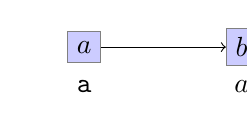
\begin{tikzpicture}
  [memory/.style={rectangle,draw=black!50,fill=blue!20}]
  \node at (0,0.5) [memory] (reference) {$a$};
  \node at (0,0) {{\tt a}};
  \node at (2,0.5) [memory] (address) {$b$};
  \node at (2,0) {$a$};
  \draw [->] (reference.east) -- (address.west);
\end{tikzpicture}
\end{center}

\subsection{Comments}
\label{s:java:comments}
A {\it comment}\index{comment} is simply text inserted in a program so
as to remind human readers of the meaning of the surrounding
instructions. Natural,\index{language!natural} rather than formal
languages,\index{language!formal} are usually employed. Comments are
supposed to make code clearer and easier to understand. A program with
no comments will probably be unreadable; on the other hand, users will
most likely ignore comments if every single line is commented.

In Java, comments can be single line or multi-line. A double slash
(``{\tt //}'') means that the rest of the line, until its end, will
contain a comment. A multi-line comment starts with ``{\tt /*}'' and
ends with ``{\tt */}''. An example of a multi-line comment is given in
the {\tt helloWorld} program.

Comments are ignored by the Java compiler,\index{compiler} but some
relevant information can be stored in comments, to be read by an
appropriate {\it preprocessor}\index{preprocessor} --- this is
software that interprets the program according to different rules, and
is usually called prior to (or independently of) the compiler. This
can be useful to automatically produce documentation for a given
software, for example.

\subsection{Classes}
A {\it class}\index{class} is the Java\index{Java} equivalent of a
mathematical set\index{set} defined by a property
$P$,\index{set!property} i.e.~$\{x\;|\;P(x)\}$. In Java, the property
$P$ is a description of the {\it data type}\index{data!type} of each
piece of data $x$ in the class, e.g.~$x$ might store an integer, a
float and a string.

In Java, every program must contain at least a class. A {\it
  class}\index{class} is the formal Java definition of a data
structure.\index{data!structure} It usually contains a list of
variable names\index{variable!name} (with associated data
type)\index{data!type} and a list of functions that determine how the
values stored in the variables change. The class in the {\tt
  helloWorld}\index{helloWorld@{\tt helloWorld}} program, called {\tt
  helloWorld}, only contains one function called {\tt
  main}.\index{main@{\tt main}}

A class is an entity which resides in the Java program. Once compiled
and executed, a class, strictly speaking, does nothing. The Java
VM,\index{virtual machine} however, may create (either by default or
because instructed to do so) {\it objects}\index{object} of any given
class. An object is therefore an instance of the class stored in
memory. If we draw a parallel between Java and mathematical language,
a class is to a set what an object is to an element. In other words, a
class is a description of the data structure, whereas an object is an
actual piece of data that is structured in memory according to the
specification of its class. For example, the class
\begin{verbatim}
class IntPair {
  int first;
  int second;
}
\end{verbatim}
defines a data structure\index{data!structure} that holds two integers
between $-2^{31}$ and $2^{31}-1$. An object {\tt myIntPair} of this
class, defined as:
\begin{verbatim}
  IntPair myIntPair = new IntPair;
\end{verbatim}
holds a pair of integers in memory. The name {\tt myIntPair} is
arbitrary --- the fact that it is similar to the class name is only
supposed to help a reader identify the class directly from the object.
In general, two different objects of the same class hold different
data.

Class members,\index{class!member} be they data ({\it
  attributes})\index{attribute} or functions ({\it
  methods}),\index{method} can some specifiers, such as {\tt
  public},\index{public} {\tt static}\index{static} and others. Public
class members can be referenced from instructions\index{instruction}
outside the class. Static members are stored at a single
address\index{memory!address} in memory, which means that all objects
of the same class all share static data.\index{data!shared} By
default, members are neither public nor static, which means that they
can only be referenced from instructions inside the class, and each
object of the class can refer to its own private\index{private} copy
of the data.

\subsubsection{The {\tt this} attribute}
Suppose the class {\tt myClass} has a method {\tt myMethod}. Within
the {\tt myMethod} code, the Java keyword {\tt this}\index{this@{\tt this}}
is a reference to the object which will execute {\tt myMethod}. This
means that two objects of the same class have the same attribute {\tt
  this}, but this will hold two different memory addresses depending
on which object refers to it. 

\subsubsection{Inheritance}\index{inheritance}\index{class!inheritance}
Just as sets can, in mathematics, be subsets of other sets, classes
can be subclasses of other classes. A class\index{class} {\tt C}
describing each of its objects\index{object} as storing an integer, a
float and a string might well be a subclass of another class {\tt B}
whose objects only store an integer and a float.

Inheritance is useful for several reasons. For example, if we need
both {\tt B} and {\tt C} in our code and do not have inheritance, we
must write
\begin{verbatim}
  public class B {
    int i;
    float f;
  }

  public class C {
    int i;
    float f;
    String s;
  }
\end{verbatim}
Notice we are duplicating some code.\index{code!duplication} If we
need to change the {\tt float} to a {\tt double} later on, and still
require {\tt B} to be a subclass of {\tt C}, we must remember to
change the code in different places: since people forget such details,
it will very likely give rise to a bug.\index{bug} Notice that a
similar type of bug destroyed the Ariane\index{Ariane 5} 5 on its
maiden flight. Inheritance helps avoid this issue. We define
{\tt C} as follows:
\begin{verbatim}
  public class C extends B {
    String s;
  }
\end{verbatim}
In other words, we explicitly tell the compiler\index{compiler} that
there is a relationship between the two classes. This not only
shortens the code, but decreases the chances of coding mistakes by
delegating to the compiler the responsibility of checking that the
relationship $\mbox{\tt C}\subseteq\mbox{\tt B}$ is maintained
throughout the code.

\subsubsection{Interfaces}
\label{s:java:interface}
An {\it interface}\index{interface}\index{class!interface} is a very
special kind of class, whose purpose is that of enforcing
conformance\index{conformance} to a certain class
structure.\index{class!structure} For example, in a Graphical User
Interface (GUI)\index{GUI} every window (including full program
windows, dialog boxes and warning boxes) must conform to certain basic
notions about windows: e.g., they possess a width, a height, a title
and a frame, they have some standard buttons for minimizing,
maximizing and closing, they have some standard pull-down menu, and
they must remember their contents so that these can be re-drawn if
another window is temporarily dragged over it. A programmer who
designs a new type of window might be tempted to design a window of a
different kind, say with no standard buttons. However, all other
programs running on the GUI automatically assume that all windows have
standard buttons, so they are free to call the associated code: in the
long run, this might cause bugs and unforeseen behaviour. To avoid
this, the compiler itself enforces conformance with a standard idea of
window in the GUI by means of an interface: all classes defining a
window must inherit from the window interface, and implement its
functions as they see fit.

Remark that interfaces have no data and only contain the names,
argument types and return types of the member functions. No object can
be defined as member of an interface class
only.\index{object!interface} By contrast, objects of different
classes that both implement\index{interface!implementation} (i.e.,
inherit from) the same interface class can both be attributed the
interface data type. Let us consider the example of a normal window
and of a special type of window whose aspect ratio is always 3:2.
\begin{verbatim}
interface Window {
  int getWidth();
  int getHeight();
}

class MainWindow implements Window {
  int width;
  int height;
  public int getWidth() {
    return width;
  }
  public int getHeight() {
    return height;
  }
}

class FixedRatioWindow implements Window {
  int size;
  public int getWidth() {
    return 3*size;
  }
  public int getHeight() {
    return 2*size;
  }
}
\end{verbatim}
In subsequent code, we might wish to loop over all windows. This is
possible thanks to inheritance from the {\tt Window} array.
\begin{verbatim}
  MainWindow mw = new MainWindow();
  FixedRatioWindow frw = new FixedRatioWindow();
  ArrayList<Window> a;
  // ...
  a.add(mw);
  a.add(frw);
  // now we can loop over the elements of a
\end{verbatim}
Notice that {\tt ArrayList<Window>}\index{ArrayList@{\tt ArrayList}}
implements an array of interfaces (we shall discuss the funny angular
brackets later, see Sect.~\ref{s:linear:map:parametrized}).

\subsection{Functions}
In general, functions\index{Java!function} may take a list of
arguments\index{function!argument} of given type, implement an
algorithm\index{algorithm} with such arguments as input, and then
optionally return a value of given type to the calling function. For
example, the Java function {\tt f} taking an integer input and
returning its square is implemented as follows.
\begin{verbatim}
int f(int x) {
  return x*x;
}
\end{verbatim}

\subsubsection{Passing by reference or value} 
Consider the mathematical function $f(x)=x^2$, and the possible
C++\index{C++} implementation:
\begin{verbatim}
dataType f(dataType x) {
  x *= x;
  return x;
}
\end{verbatim}
(we remark this is a valid construct in Java too, but we refer to C++
here for technical reasons). The {\tt dataType} keyword is simply the
data type of the argument {\tt x} and of the return\index{return
  value} value of {\tt f}. It might describe an integer\index{integer}
or a floating-point\index{floating-point} number.

Now consider a calling function:
\begin{verbatim}
void g() {
  dataType x = 2;
  dataType y = f(x);
  cout << x << " + **2 = " << y << endl; // print string on screen
}
\end{verbatim}
and try and imagine what the printed output will be like. Obviously,
{\tt y} will take value 4. But what value will {\tt x} take? The
definition of {\tt f} changes the value of {\tt x}, but will this
change be remembered in the calling function?

The answer depends on whether {\tt f} has access to the value of {\tt
  x}, or to the address\index{address} where {\tt x} is stored in
memory.\index{memory} In the first case, this value will be stored by
{\tt f} in a new memory area: the {\tt x} in {\tt g} and the {\tt x}
in {\tt f} are stored in two distinct memory cells, whose values can
be changed independently. in the second case, if {\tt f} changes the
value of {\tt x}, {\tt g} will retrieve the changed value, because
{\tt x} in {\tt f} and {\tt x} in {\tt g} are stored at the same
memory address. In the first case, {\tt x} is {\it passed by
  value},\index{passing!by value}\index{value!passing by} and in the
second, {\tt x} is {\it passed by reference}\index{passing!by
  reference}.\index{reference!passing by}

In Java, passing by value or by reference is not a user choice.
Elementary data types\index{data!type!elementary} ({\tt boolean}, {\tt
  int}, {\tt long}, {\tt float}, {\tt double}, {\tt char}) are passed
by value, and all other data types (including user-defined classes)
are passed by reference.

\subsubsection{The {\tt main} function}
The function {\tt main}\index{main@{\tt main}} takes as argument an
array\index{array} called {\tt args},\index{args@{\tt args}} and
returns no data --- this is the meaning of the {\tt
  void}\index{void@{\tt void}} right before the function declaration.
In the case of the {\tt helloWorld} program, all it does is to print
out to the system screen the string ``hello world''.

\subsubsection{Specifiers}
Some details about how functions are translated to executable code by
the Java compiler\index{Java!compiler}\index{compiler} can be
influenced by code {\it specifiers}.\index{specifier}

The {\tt main} function of the {\tt helloWorld} program, for example,
is specified to be {\tt public} and {\tt static}. The first specifier,
{\tt public},\index{public} states that this function can be called
from other functions, even outside the class (normally, functions in a
class can only be called by other functions in the same class). The
second specifier, {\tt static},\index{static} tells the
compiler\index{compiler} that any object of the class {\tt helloWorld}
will share a single copy of the {\tt main}\index{main@{\tt main}} function:
the function code will be stored at a precise address in
memory,\index{memory!address} and this address will be stored in every
object\index{object} of the class {\tt helloWorld}. Functions and
variables that are declared {\tt static}\index{static} serve a purpose
of sharing data between different objects of the same class.

\subsection{Data types}
A class defines the type of data it encodes: if an object is a piece
of data, the class it belongs to is the {\it data
  type}.\index{data!type} In Java, we distinguish a small set of data
types, which includes {\tt boolean},\index{boolean@{\tt boolean}} {\tt
  int},\index{int@{\tt int}} {\tt long},\index{long@{\tt long}} {\tt
  float},\index{float@{\tt float}} {\tt double}\index{double@{\tt
    double}} and {\tt char}:\index{char@{\tt char}} these are called {\it
  elementary}.\index{data!type!elementary} Elementary data types do
not correspond to any defined class --- rather, these types are
hard-coded in the compiler.\index{compiler} This makes a difference as
far as functions are concerned. The instruction
\begin{verbatim}
void f(int a);
\end{verbatim}
will define a function called {\tt f} which takes as input an {\tt
  int} called {\tt a}. If the function {\tt f} changes the value
stored in {\tt a}, this has no effect on {\tt a} outside the function:
\begin{verbatim}
  int a = 2;
  f(a);
  System.out.println(a);
  // ...
  void f(int a) {
    a = 1;
  } 
\end{verbatim}

\subsection{The dot operator}
For Java instructions to refer to the
member\index{object!member}\index{member} {\tt first} of the object
{\tt myIntPair}, the dot\index{dot operator}\index{operator!dot}
operator is used, e.g.:
\begin{verbatim}
  myIntPair.first = 1;
\end{verbatim}
With this in mind, it is easy to interpret the instruction
\begin{verbatim}
  System.out.println("hello world");
\end{verbatim}
as a chain of embedded objects: it is a call to the function {\tt
  println}, which is in the object {\tt out},\index{System.out@{\tt System.out}}
which is itself one of the data in the object 
{\tt System}.\index{System@{\tt System}}

\subsection{The curly brackets}
In Java (and also in C\index{C} and C++),\index{C++} curly
brackets,\index{bracket!curly}\index{\{\}} (also known as
braces),\index{brace} are used to delimit the scope\index{scope} of a
set of instructions. Accordingly, they mark the beginning and end of a
class, function, but also of {\tt if} blocks\index{block!if}, and {\tt
  while}\index{block!while} and {\tt for}\index{block!for}
loops.\index{loop}

\subsection{The semicolon}
Every basic instruction\index{instruction!basic} in Java is terminated
by a semicolon.\index{;}\index{semicolon} Notice that a basic
instruction does not necessarily correspond to a line. Class or
function definitions are not considered basic instructions, insofar as
they are delimited by braces rather than ended by a semicolon.

\subsection{How code is executed}
A program can include several classes, defined in different
files.\index{file} However, for a program to yield executable
code,\index{code!executable} there must be a {\it point of
  entry},\index{point of entry} i.e.~a first function that the
Operating System\index{operating system} (OS)\index{OS} knows it can
call. This function can then call all the other functions in the
program. In Java, this first function is called {\tt main},\index{main@{\tt
    main}} it must be defined as {\tt static}\index{static} and {\tt
  void},\index{void} it takes as input the list of command line
arguments passed by the user to the program via the shell\index{shell}
prompt, and must be a {\tt public}\index{public} class
member.\index{class!member} Moreover, the name of the class containing
{\tt main} should have the same name as the Java file\index{file} it
is stored in (see the {\tt helloWorld} example).

\section{Arrays in Java}
\label{s:java:array}
An {\it array}\index{array} represents a list of objects\index{object}
of the same class. An example of an array of three {\tt int} having
value $2,1,-1$ is shown below.
\begin{center}
\fbox{2}\fbox{1}\fbox{-1}
\end{center}
The fact that the objects come one after the other is meant to suggest
that they are stored in memory at contiguous addresses. This may be
true or not, depending on the actual array implementation. It is
usually true to a degree: an array might well be implemented as a set
of distinct memory segments, each of which consists of contiguous
addresses. 

\subsection{Dimensions}
Arrays can be {\it linear}\index{array!linear} or {\it
  multidimensional}.\index{array!multidimensional} Mathematically
speaking, a linear array is similar to a vector,\index{vector} a
two-dimensional\index{array!two-dimensional} array to a
matrix,\index{matrix} and a multidimensional array to a
tensor.\index{tensor}

\subsection{The square bracket notation}
In Java, arrays are declared using square
brackets,\index{bracket!square} in one of the two ways below.
\begin{verbatim}
int[] myArray;
int myArray[];
\end{verbatim}
Declaring an array does not make it usable: first, we must allocate
some memory\index{memory!allocation} to it.
\begin{verbatim}
myArray = new int[4]; // reserves enough memory to hold 4 int
\end{verbatim}
It is common to combine the declaration and the memory allocation in
the same instruction (both alternatives will work).
\begin{verbatim}
int[] myArray = new int[4];
int myArray[] = new int[4];
\end{verbatim}
Multidimentional arrays get as many square bracket pairs as there are
dimensions.\index{dimension} The following defines a $(4\times 3\times
2)$ 3-dimensional array of {\tt int}.
\begin{verbatim}
int[][] x = new int[4][3][2];
\end{verbatim}
In Java, the number of components\index{component} in each dimension
need not be a constant. 
\begin{verbatim}
int n = 2;
int m = 3;
int[][][] x = new int[4][m][n];
\end{verbatim}


\section{Example: plotting the graph of a function}
In this section we shall present a simple worked-out Java example,
consisting entirely of static data, that plots\index{function!plot} a
function $y=f(x)$ of one variable on a text console\index{console}
screen. This program consists of a single class,\index{class} called
{\tt functionPlot},\index{functionPlot@{\tt functionPlot}} and resides
in a single file called {\tt functionPlot.java}. The class is declared
static\index{static} and contains a {\tt main}\index{main@{\tt main}}
function, as detailed above. The {\tt main} function performs the
following tasks:
\begin{enumerate}
\item initialize some data, such as the ranges $[x^L,x^U]$ where we
  wish to tabulate $f(x)$, the number $n$ of function table entries,
  as well as the size of the ``text screen'' (number of
  rows\index{row} and columns);\index{column}
\item compute two vectors:\index{vector} $(x_1,\ldots,x_n)$ such that
  $x_k\in[x^L,x^U]$ for all $k\le n$, and $(y_1,\ldots,y_n)$ such that
  $y_k=f(x_k)$ for all $k\le n$;
\item fill an integer\index{integer} array\index{array} {\tt screen}
  with zeroes, apart from those entries $(i,j)$ (set to 1) that best
  approximate the pairs $(x_k,y_k)$;
\item print the array {\tt screen} on the text console.\index{console}
\end{enumerate}

\subsection{A typical output}
\label{s:java:example:output}
A typical output with 20 rows, 75 columns, and
$f(x)=\frac{1}{4}x+\sin(x)$ in the range $[-10,10]$ is shown in
Fig.~\ref{f:fplot}.
\begin{figure}[!ht]
\begin{center}
\fbox{\begin{minipage}{13cm}
{ \small
  \verbatiminput{functionPlot.out}
}
\end{minipage}}
\end{center}
\caption{A typical output from {\tt functionPlot}.}
\label{f:fplot}
\end{figure}

\subsection{Comments and imports}
The {\tt filePlot.java} file starts with the usual
comments\index{comment} bearing some minimal information about the
program.
\begin{verbatim}
/*
  Name: functionPlot.java
  Purpose: plotting functions in ASCII
  Author: Leo Liberti
  Source: Java
  History: 120615 work started
*/
\end{verbatim}

Next, we {\it import}\index{import} some standard Java classes.
\begin{verbatim}
import java.io.*;
import java.util.*;
import java.lang.*;
\end{verbatim}
The {\tt import} command tells the compiler to read some other Java
code, which might include declarations\index{declaration} and
definitions\index{definition} of names occurring in the program. For
example, we shall make use of mathematical functions {\tt
  Math.sin}\index{sine} and {\tt Math.rint},\index{integer rounding}
as well as the print\index{print} functions {\tt
  System.out.print}\index{System.out@{\tt System.out}} and {\tt
  System.out.println}. We shall not explicitly declare these
functions, but rather instruct the compiler to look for them in some
standard libraries.\index{library!standard}

\subsection{The class declaration}
We present the class structure\index{class!structure} next. We remark
that the following class contains some function {\it
  declarations}\index{declaration} (specifiers, return type, name,
argument types) without the corresponding {\it
  definition}\index{definition} (the function code, contained in
braces);\index{brace} accordingly, the following code cannot be
compiled ``as is'': all function declarations need to be followed by
the corresponding definitions.  {\small
\begin{verbatim}
class functionPlot {
    //// Private data
    static int steps;    // number of function evaluations
    static double [] x;  // x coordinate values
    static double xL;    // lower bound for x coordinate values
    static double xU;    // upper bound for x coordinate values
    static double [] y;  // y coordinate values
    static double yL;    // lower bound for y coordinate values
    static double yU;    // upper bound for y coordinate values
    static int rows;     // number of text rows taken by plot
    static int columns;  // number of text columns taken by plot
    static int[][] screen;
    //// Public functions
    // this defines the function to be plotted
    public static double theFunction(double z);
    // initialize some values
    public static void initialize();
    // compute the x-y table
    public static void functionTable();
    // compute the minimum value of the y range
    public static double yMin();
    // compute the maximum value of the y range
    public static double yMax();
    // fill the screen array cells corresponding to x/y pairs with 1's
    public static void tableScreen();
    // loop over the screen array and either print a '*' (1) or a space (0)
    public static void printScreen();
    // this is the program's point of entry
    public static void main(String [] args);
}
\end{verbatim}
}

All the data in the {\tt functionPlot} class is declared {\tt
  static}. This implies that all data is shared\index{data!shared}
among all functions in the class. The first section of the class
declares a set of (private)\index{private} attributes\index{attribute}
which can only be accessed by functions within the class. There
follows a section containing the (public)\index{public} declarations
of all class functions.\index{class!function} Notice that the last
function {\tt main} is the point of entry\index{point of entry} of the
VM\index{virtual machine} when it executes the code. Every line is
commented for clarity.

\subsection{The {\tt main} function}
The {\tt main} function simply calls four other functions in order:
data initialization, function tabulation, filling of the {\tt screen}
array, and printing of the {\tt screen} array on the
console\index{console} screen.
\begin{verbatim}
    public static void main(String [] args) {
        initialize();
        functionTable();
        tableScreen();
        printScreen();
    }
\end{verbatim}

\subsection{Initialization}
The {\tt initialize} function simply assigns some
user-defined\index{user} constants to some parameter variables. Users
can change the behaviour of the program in certain ways by changing
these parameters, re-compiling and re-executing the program.
\begin{verbatim}
    public static void initialize() {
        // user: set values for steps, x range, rows/columns for plot
        steps = 150;   // 150 entries in function table
        xL = -10;      // lower bound for x range
        xU = 10;       // upper bound for x range
        columns = 75;  // number of columns on the console screen
        rows = 20;     // number of rows on the console screen
        // user: do not change anything beyond this point
        x = new double[steps];  // the x vector
        y = new double[steps];  // the y vector
    }
\end{verbatim}

\subsection{Function tabulation}
Tabulating a function $f$ of one variable means computing a set of
pairs $(x_k,y_k)$ such that $y_i=f(x_k)$, for $k\le n$ where
$n\in\mathbb{N}$ is given. Accordingly, we set up two linear
arrays\index{array!linear} {\tt x}, {\tt y} to hold {\tt steps} values
each.
\begin{verbatim}
    public static void functionTable() {
        double theStep = (xU - xL) / steps;
        x[0] = xL;
        for(int k = 1; k < steps; k++) {
            x[k] = x[k-1] + theStep;
            y[k] = theFunction(x[k]);
        }	
    }
\end{verbatim}
The function {\tt functionTable} calls another function, {\tt
  theFunction}, which is simply a user-changeable\index{user}
implementation of the mathematical function $f(x)$. For example, if
$f(x)=\frac{1}{4}x+\sin x$, we have
\begin{verbatim}
    public static double theFunction(double z) {
        // user: change the mathematical function here at leisure
        return 0.25*z + Math.sin(z); 
    }
\end{verbatim}
Notice here that we use the symbol {\tt z} instead of $x$ because we
already used a static variable\index{variable!static} {\tt x} to
denote the array\index{array} storing the first
components\index{components} of the function table pairs. Since {\tt
  x} is a static variable, every function in the class (including {\tt
  theFunction} can read it and change it. Had we used {\tt double x}
instead of {\tt double z} here, we would have {\it
  shadowed}\index{shadowing} the symbol {\tt x} that denotes the
array, rendering it inaccessible within this function. Also notice the
library function\index{library} {\tt sin}, which is a member function
of the class {\tt Math}.\index{Math@{\tt Math}}

\subsection{Converting the function table to an array}
We pave the way for printing\index{print} to the
console\index{console} screen. We model this screen by means of a
two-dimensional array\index{array!two-dimensional} {\tt screen},
indexed on rows\index{row} and columns.\index{column} Initially, we
fill {\tt screen} with zeroes. Later on, we loop\index{loop} over the
function table pairs, and we change {\tt screen}'s $(i,j)$-th entry to
a one whenever there is a pair $(x_k,y_k)$ such that $(i,j)$ is the
best integer approximation of $(x_k,y_k)$ (after appropriate
translation and scaling). More precisely, we let:
\begin{eqnarray*}
   j &=& \left\lfloor \frac{x_k-x^L}{x^U-x^L}\sigma +
   \frac{1}{2}\right\rfloor\\
   i &=& \left\lfloor \frac{y_k-y^L}{y^U-y^L}\rho +
   \frac{1}{2}\right\rfloor,
\end{eqnarray*}
where $\sigma$ is the number of columns ({\tt columns} in the code)
and $\rho$ the number of rows ({\tt rows} in the code. Adding
$\frac{1}{2}$ to a real number and taking its floor\index{floor} is
the same as rounding\index{integer rounding} it to the closest
integer.
\begin{verbatim}
    public static void tableScreen() {
        int i;
        int j;
        screen = new int [rows][columns];
        for(i = 0; i < rows; i++) {
            for(j = 0; j < columns; j++) {
                 screen[i][j] = 0;
            }
        }
        yL = yMin();
        yU = yMax();
        for(int k = 0; k < steps; k++) {
            j = (int) Math.rint(((x[k] - xL) / (xU - xL)) * columns);
            i = (int) Math.rint(((y[k] - yL) / (yU - yL)) * rows);
            if (i < rows && j < columns) {
                 screen[rows - (i + 1)][j] = 1;
            }
        }
    }
\end{verbatim}
The above function calls two other functions, {\tt yMin} and {\tt
  yMax}, that compute the minimum\index{minimum} and
maximum\index{maximum} of the $y$ range, and are defined as follows.
\begin{verbatim}
    public static double yMin() {
        double theMin = 1e30; // infinity
        for(int k = 0; k < steps; k++) {
            if (y[k] < theMin) {
                theMin = y[k];
            }
        }
        return theMin;
    }
    public static double yMax() {
        double theMax = -1e30; // -infinity
        for(int k = 0; k < steps; k++) {
            if (y[k] > theMax) {
                theMax = y[k];
            }
        }
        return theMax;
    }
\end{verbatim}

\subsection{Printing the screen}
We now come to the function that copies the arrays\index{array} {\tt
  screen} onto the console\index{console} screen. We interpret it so
that every time {\tt screen} contains a 1, a `{\tt *}' is printed on
the screen, while all zeroes are printed as spaces.
\begin{verbatim}
    public static void printScreen() {
        for(int i = 0; i < rows; i++) {
            for(int j = 0; j < columns; j++) {
                if (screen[i][j] == 1) {
                    System.out.print("*");
                } else {
                    System.out.print(" ");
                }
            }
            System.out.print("\n");
        }
    }
\end{verbatim}

\subsection{Compilation and running}
As for {\tt helloWorld}, the program {\tt functionPlot} can be
compiled and executed very simply as follows.
\begin{verbatim}
javac functionPlot.java
java functionPlot
\end{verbatim}
The output of {\tt functionPlot} with the user-defined\index{user}
parameters is given in Sect.~\ref{s:java:example:output}

\begin{ex}
Extend the {\tt functionPlot} class so that it also prints the $x$ and
$y$ axes.
\end{ex}

%%%%%%%%%%%%%%%%%%%%%%%%%%%%%%%%%%%%%%%%%%%%%%
%%%%%%%%%%%%%%%%% PART II %%%%%%%%%%%%%%%%%%%%
%%%%%%%%%%%%%%%%%%%%%%%%%%%%%%%%%%%%%%%%%%%%%%

\part{Data structures}

%%%%%%%%%%%%%%%%%%%%%%%%%% CHAPTER: GRAPHS %%%%%%%%%%%%%%%%%%%%%%%%%%%%%

%% TODO in this chapter: add some references

\chapter{Graphs}
\label{c:graph}

\begin{center}
\fbox{\begin{minipage}{13cm}{\small {\sc Abstract}.  
Directed and undirected graphs, neighbourhoods, complements, line
graphs, graph isomorphism. Subgraphs, stables and
cliques. Connectivity: paths and cycles. Basic operations on graphs.
}
\end{minipage}}
\end{center}

Data structures\index{data!structure} consist of pieces of data as
well as relations\index{relation} between and among them. We are going
to formalize this concept mathematically by means of
graphs.\index{graph} Graphs are also the appropriate mathematical
model for networks, be they transportation, communication, power,
social or other types of networks. Learning the ropes of graph theory
will therefore serve a double purpose.

\section{Directed graphs}
\label{s:graph:directed}
Formally, a {\it relation} on a set $V$ is a subset of the Cartesian
product\index{Cartesian product} $V\times V$ of all ordered pairs of
elements of $V$. Accordingly, we define a {\it directed
  graph}\index{graph!directed} (or {\it digraph})\index{digraph} as a
pair $G=(V,A)$ where $V$ is the set of {\it nodes}\index{node} (or
{\it vertices})\index{vertex} and $A$, a subset of $V\times V$, is
the set of {\it arcs}\index{arc} of the graph. Given a digraph $G$, we
sometimes denote its node set by $V(G)$ and arc set by $A(G)$. 
\begin{figure}[!ht]
\begin{center}
\begin{minipage}{3.5cm}
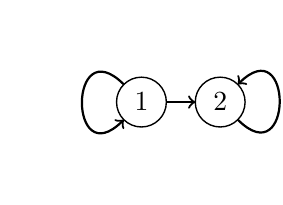
\begin{tikzpicture}
%\useasboundingbox (-1,-2) rectangle (8,2);
\SetVertexNormal
\SetGraphUnit{1}
\Vertex{1}
\EA(1){2}
\Edge[style={->}](1)(2)
\Loop[dist=1cm,dir=EA,style={->}](2)
\Loop[dist=1cm,dir=WE,style={->}](1)
\end{tikzpicture}
\end{minipage}
\begin{minipage}{3.5cm}
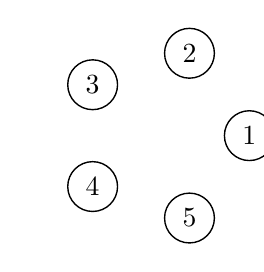
\begin{tikzpicture}
\GraphInit[vstyle=Normal]
\SetGraphUnit{1.1}
\tikzset{EdgeStyle/.append style={->}}
\Vertices{circle}{1,2,3,4,5}
\end{tikzpicture}
\end{minipage}
\begin{minipage}{3cm}
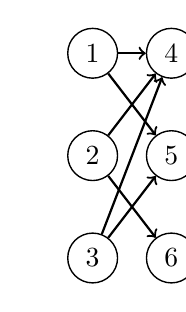
\begin{tikzpicture}
\GraphInit[vstyle=Normal]
\SetGraphUnit{1.3}
\tikzset{EdgeStyle/.append style={->}}
\Vertices[dir=\SO,x=0,y=0]{line}{1,2,3}
\Vertices[dir=\SO,x=1,y=0]{line}{4,5,6}
\Edge(1)(4)
\Edge(1)(5)
\Edge(2)(4)
\Edge(2)(6)
\Edge(3)(4)
\Edge(3)(5)
\end{tikzpicture}
\end{minipage}
\begin{minipage}{4cm}
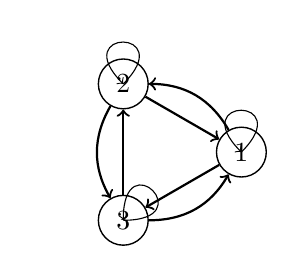
\begin{tikzpicture}
\GraphInit[vstyle=Normal]
\SetGraphUnit{1}
\tikzset{EdgeStyle/.style={->,bend right}}
\Vertices{circle}{1,2,3}
\Loop[dist=1cm,dir=EA,style={->}](1)
\Loop[dist=1cm,dir=EA,style={->}](2)
\Loop[dist=1cm,dir=SOEA,style={->}](3)
\Edges(1,2,3,1)
\tikzset{EdgeStyle/.style={->}}
\Edges(1,3,2,1)
\tikzset{EdgeStyle/.style={->,bend right}}
\end{tikzpicture}
\end{minipage}
\end{center}
\caption{Examples of digraphs.}
\label{fig:digraphs}
\end{figure}
A reflexive relation pair $(v,v)$ is a special type of arc called a
{\it loop}\index{loop}, see e.g.~the loops $(1,1)$ and $(2,2)$ in the
leftmost graph of Fig.~\ref{fig:digraphs}. A {\it
  multidigraph}\index{multidigraph} associates a positive integer to
each arc called its {\it multiplicity}.\index{arc!multiplicity} An arc
with multiplicity higher than one is a {\it multiple
  arc}.\index{arc!multiple} A digraph is {\it
  simple}\index{digraph!simple} if it has no loops or multiple arcs.
A digraph is {\it empty}\index{digraph!empty} if its arc set is empty
(e.g.~second digraph from the left in Fig.~\ref{fig:digraphs}).  A
digraph is {\it bipartite}\index{bipartite}\index{digraph!bipartite}
if its node set $V$ can be partitioned in two sets $U,W$ such that
every arc $(u,w)\in A$ has $u\in U$ and $w\in W$ (e.g.~third digraph
from the left in Fig.~\ref{fig:digraphs}). A digraph is {\it
  complete}\index{digraph!complete}\index{complete} if its arc set is
$V\times V$ (e.g.~last digraph from the left in
Fig.~\ref{fig:digraphs}). Complete digraphs are also called {\it
  directed cliques}.\index{clique!directed}

\subsection{Directed neighbourhoods}
Given a digraph $G=(V,A)$ and a node $u\in V$, the node set
$N^+_G(u)=\{v\in V\;|\;(u,v)\in A\}$ is called the \textit{outgoing
  neighbourhood}\index{neighbourhood!outgoing} of $u$ with respect to
$G$. The node set $N^-_G(u)=\{v\in V\;|\;(v,u)\in A\}$ is called the
\textit{incoming neighbourhood}\index{star!neighbourhood} of $u$ with
respect to $G$ (see Fig.~\ref{fig:star}).
\begin{figure}[!ht]
\begin{center}
\psfrag{d-}{$N^-(7)$}
\psfrag{d+}{$N^+(7)$}
\includegraphics[width=5cm]{stars}
\end{center}
\caption{Incoming and outgoing neighbourhoods of node 7:
  $N^-(7)=\{1,2,3\}$ and $N^+(7)=\{4,5,6\}$.}
\label{fig:star}
\end{figure}
The \textit{outdegree}\index{outdegree} of a node $v\in V$ is the
cardinality of its outgoing neighbourhood, and similarly, the
\textit{indegree}\index{indegree} of $v\in V$ is the cardinality of
its incoming neighbourhood. In Fig~\ref{fig:star}, both the indegree
and the outdegree of node 7 are equal to 3. For $u\in V$, the arc set
$\delta^+_G(u)=\{(v,w)\in A\;|\;u=v\}$ is called {\it outgoing
  star}\index{star!outgoing} (or {\it outstar})\index{outstar} of $u$
with respect to $G$, and the arc set $\delta^-_G(u)=\{(w,v)\in
A\;|\;u=v\}$ is called {\it incoming star}\index{star!incoming} (or
{\it instar})\index{instar} of $u$ with respect to $G$. If there is no
ambiguity we dispense with the index $G$.

\section{Undirected graphs}
\label{s:graph:undirected}
Essentially, a graph is like a digraph where all arrows are replaced
by segments. More formally, a {\it graph}\index{graph} is a pair
$G=(V,E)$ where $V$ is a set of vertices and $E$ is a set of {\it
  edges}\index{edge} $\{u,v\}$ where $u,v\in V$. As for digraphs, for
a graph $G$ we sometimes denote by $V(G)$ its vertex set and by $E(G)$
its edge set. Whenever $u=v$ then $\{u,v\}=\{u\}=\{v\}$ is called a
loop. In {\it multigraphs},\index{multigraph} a positive integer
called multiplicity is assigned to each edge; edges with multiplicity
higher than one are called multiple (or parallel) edges (see
Fig.~\ref{fig:multigraph}). A graph without loops or multiple edges is
called {\it simple}.\index{graph!simple}
\begin{figure}[!ht]
\begin{center}
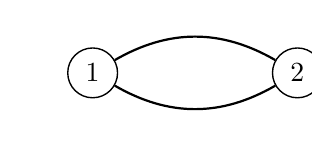
\begin{tikzpicture}[scale=1.3]
\SetGraphUnit{2}
\GraphInit[vstyle=Normal]
\tikzset{LabelStyle/.style= {draw,fill = yellow,text = red}}
\Vertex[L={$1$}]{A}
\EA[L={$2$}](A){B}
\tikzset{EdgeStyle/.append style = {bend left}}
\Edge(A)(B)
\tikzset{EdgeStyle/.append style = {bend right}}
\Edge(A)(B)
\end{tikzpicture}
\end{center}
\caption{A multigraph with two parallel edges.}
\label{fig:multigraph}
\end{figure}
Given a digraph, its \textit{underlying graph}\index{graph!underlying}
replaces every arc $(u,v)$ with the corresponding edge $\{u,v\}$ (see
Fig.~\ref{f:underlying}).
\begin{figure}[!ht]
\begin{center}
\begin{minipage}{5cm}
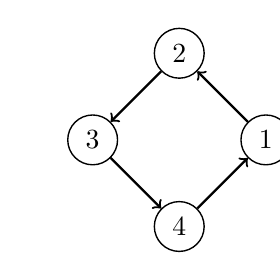
\begin{tikzpicture}[scale=1]
\GraphInit[vstyle=Normal]
\SetGraphUnit{1.1}
\tikzset{EdgeStyle/.append style={->}}
\Vertices{circle}{1,2,3,4}
\Edges(1,2,3,4,1)
\end{tikzpicture} 
\end{minipage}
\hspace*{1cm}
\begin{minipage}{5cm}
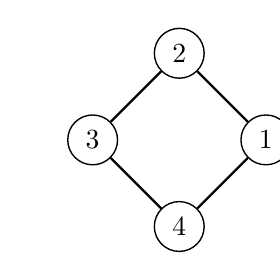
\begin{tikzpicture}[scale=1]
\GraphInit[vstyle=Normal]
\SetGraphUnit{1.1}
\Vertices{circle}{1,2,3,4}
\Edges(1,2,3,4,1)
\end{tikzpicture} 
\end{minipage}
\end{center}
\caption{A digraph and its underlying graph.}
\label{f:underlying}
\end{figure}
A graph is {\it empty}\index{graph!empty} if its edge set is empty. A
graph is {\it complete}\index{complete graph}\index{graph!complete}
(or a {\it clique})\index{clique} if every possible edge $\{u,v\}$ is
in $E$ for all $u\not=v\in V$. Notice that complete graphs are
simple. A graph $G=(V,E)$ is {\it
  bipartite}\index{bipartite}\index{graph!bipartite} if $V$ can be
partitioned in two sets $U,W$ such that every edge $\{u,w\}\in E$ has
$u\in U$ and $w\in W$.

\subsection{Complement graphs}
Given a graph $G=(V,E)$, consider the clique\index{clique} $K(V)$ on
$V$ with edge set\index{edge!set} $E_K$ consisting of all possible
vertex pairs.\index{vertex!pair} The graph $\bar{G}=(V,\bar{E})$,
where $\bar{E}=E_K\smallsetminus E$ is the {\it complement
  graph}\index{graph!complement} of $G$ (Fig.~\ref{f:complement}).
\begin{figure}[!ht]
\begin{center}
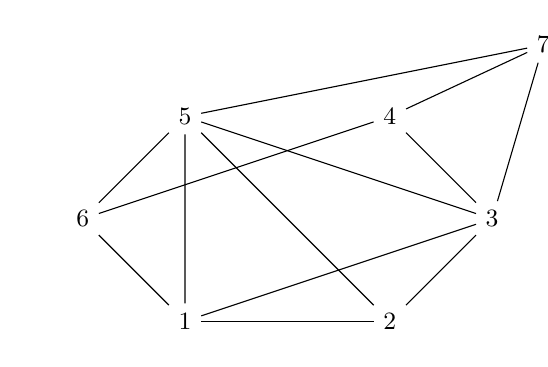
\begin{tikzpicture}[scale=1.3]
\node (v1) at (1,0) {\small $1$} ;
\node (v2) at (3,0) {\small $2$} ;
\node (v3) at (4,1) {\small $3$} ;
\node (v4) at (3,2) {\small $4$} ;
\node (v5) at (1,2) {\small $5$} ;
\node (v6) at (0,1) {\small $6$} ;
\node (v7) at (4.5,2.7) {\small $7$} ;
\draw (v1) to [thick] (v2) ;
\draw (v1) to [thick] (v3) ;
%\draw (v1) to [color=white] (v4) ;
\draw (v1) to [thick] (v5) ;
\draw (v1) to [thick] (v6) ;
%\draw (v1) to [color=white] (v7) ;
\draw (v2) to [thick] (v3) ;
%\draw (v2) to [color=white] (v4) ;
\draw (v2) to [thick] (v5) ;
%\draw (v2) to [color=white] (v6) ;
%\draw (v2) to [color=white] (v7) ;
\draw (v3) to [thick] (v4) ;
\draw (v3) to [thick] (v5) ;
%\draw (v3) to [color=white] (v6) ;
\draw (v3) to [thick] (v7) ;
%\draw (v4) to [color=white] (v5) ;
\draw (v4) to [thick] (v6) ;
\draw (v4) to [thick] (v7) ;
\draw (v5) to [thick] (v6) ;
\draw (v5) to [thick] (v7) ;
%\draw (v6) to [color=white] (v7) ;
\end{tikzpicture}
\hspace*{1cm}
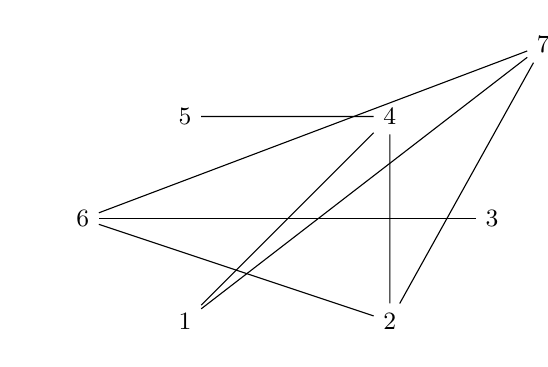
\begin{tikzpicture}[scale=1.3]
\node (v1) at (1,0) {\small $1$} ;
\node (v2) at (3,0) {\small $2$} ;
\node (v3) at (4,1) {\small $3$} ;
\node (v4) at (3,2) {\small $4$} ;
\node (v5) at (1,2) {\small $5$} ;
\node (v6) at (0,1) {\small $6$} ;
\node (v7) at (4.5,2.7) {\small $7$} ;
%\draw (v1) to [color=white] (v2) ;
%\draw (v1) to [color=white](v3) ;
\draw (v1) to [thick] (v4) ;
%\draw (v1) to [color=white] (v5) ;
%\draw (v1) to [color=white] (v6) ;
\draw (v1) to [thick] (v7) ;
%\draw (v2) to [color=white] (v3) ;
\draw (v2) to [thick] (v4) ;
%\draw (v2) to [color=white] (v5) ;
\draw (v2) to [thick] (v6) ;
\draw (v2) to [thick] (v7) ;
%\draw (v3) to [color=white] (v4) ;
%\draw (v3) to [color=white] (v5) ;
\draw (v3) to [thick] (v6) ;
%\draw (v3) to [color=white] (v7) ;
\draw (v4) to [thick] (v5) ;
%\draw (v4) to [color=white] (v6) ;
%\draw (v4) to [color=white] (v7) ;
%\draw (v5) to [color=white] (v6) ;
%\draw (v5) to [color=white] (v7) ;
\draw (v6) to [thick] (v7) ;
\end{tikzpicture}
\end{center}
\caption{A graph and its complement.}
\label{f:complement}
\end{figure}

\begin{ex}
Propose an $O(n+m)$ algorithm for constructing the complement graph of a given
graph.
\label{ex:complement}
\end{ex}

\subsection{Neighbourhoods}
Given a graph $G=(V,E)$ and a vertex $v\in V$, we let $N_G(v)=\{u\in
V\;|\;\{u,v\}\in E\}$ be the {\it neighbourhood}\index{neighbourhood}
of $v$ and $\delta_G(v)=\{\{u,w\}\in E\;|\;u=v\}$ be the {\it
  star}\index{star} of $v$ in $G$. If there is no ambiguity, we
dispense with the index $G$.

\subsection{Graph isomorphism}
Two graphs $G=(V,E)$ and $G'=(V,E')$ on the same vertex
set\index{vertex!set} $V$ are {\it
  isomorphic}\index{graph!isomorphism} if there is a
bijection\index{bijection} $\pi:V\to V$ (also called an {\it
  automorphism}\index{automorphism} on $V$) such that:
\begin{equation*}
 \forall \{u,v\}\in E \ (\{\pi(u),\pi(v)\}\in E').
\end{equation*}
In other words, changing the vertex labels\index{vertex!label} does
not change the graph structure (see
Fig.~\ref{f:graphisom}).\index{graph!structure} Since $V$ is taken to
be finite, $\pi$ is also a permutation of $V$ (see
Sect.~\ref{s:recursion:permutation}).
\begin{figure}[!ht]
\begin{center}
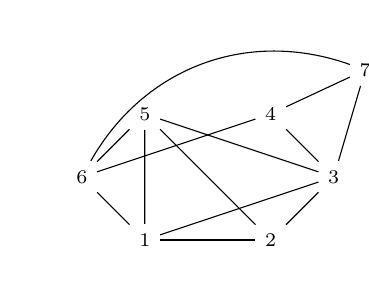
\begin{tikzpicture}[scale=0.8]
\node (v1) at (1,0) {\scriptsize $1$} ;
\node (v2) at (3,0) {\scriptsize $2$} ;
\node (v3) at (4,1) {\scriptsize $3$} ;
\node (v4) at (3,2) {\scriptsize $4$} ;
\node (v5) at (1,2) {\scriptsize $5$} ;
\node (v6) at (0,1) {\scriptsize $6$} ;
\node (v7) at (4.5,2.7) {\scriptsize $7$} ;
\draw (v1) to (v2) ;
\draw (v1) to (v3) ;
\draw (v1) to (v5) ;
\draw (v1) to (v6) ;
\draw (v2) to (v3) ;
\draw (v2) to (v5) ;
\draw (v3) to (v4) ;
\draw (v3) to (v5) ;
\draw (v3) to (v7) ;
\draw (v4) to (v6) ;
\draw (v4) to (v7) ;
\draw (v5) to (v6) ;
\draw (v6) to [bend left=40] (v7) ;
\end{tikzpicture}
$\stackrel{\scriptsize \pi=(1\to 2\to 3\to 4\to 5\to 6\to 7\to 1)}{\longrightarrow}$
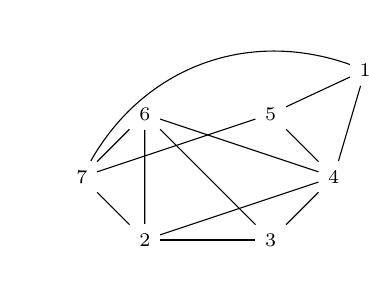
\begin{tikzpicture}[scale=0.8]
\node (v1) at (1,0) {\scriptsize $2$} ;
\node (v2) at (3,0) {\scriptsize $3$} ;
\node (v3) at (4,1) {\scriptsize $4$} ;
\node (v4) at (3,2) {\scriptsize $5$} ;
\node (v5) at (1,2) {\scriptsize $6$} ;
\node (v6) at (0,1) {\scriptsize $7$} ;
\node (v7) at (4.5,2.7) {\scriptsize $1$} ;
\draw (v1) to (v2) ;
\draw (v1) to (v3) ;
\draw (v1) to (v5) ;
\draw (v1) to (v6) ;
\draw (v2) to (v3) ;
\draw (v2) to (v5) ;
\draw (v3) to (v4) ;
\draw (v3) to (v5) ;
\draw (v3) to (v7) ;
\draw (v4) to (v6) ;
\draw (v4) to (v7) ;
\draw (v5) to (v6) ;
\draw (v6) to [bend left=40] (v7) ;
\end{tikzpicture}
\end{center}
\caption{The left graph is isomorphic to the right graph.}
\label{f:graphisom}
\end{figure}
We denote the application of $\pi$ to $G$ by $\pi G$. If $\pi G=G$,
then $\pi$ is an {\it graph
  automorphism}\index{graph!automorphism}\index{automorphism!graph} of
$G$. 

\begin{ex}
Verify that $\pi=(1\to 2\to 3\to 4\to 5\to 6\to 7\to 1)$ is not an
automorphism on the graph on the left of Fig.~\ref{f:graphisom}.
\end{ex}
The set of all graph automorphisms of a graph $G$ forms a {\it
  group}\index{group} with respect to the composition of bijections.
\begin{ex}
Verify that both $(1\to 5)$ is a graph automorphism of the graph on
the left of Fig.~\ref{f:graphisom}. Show that this graph has four
automorphisms (including the identity,\index{identity} which fixes
every $v\in V$), and, if you know what it means, that the structure of
its group\index{group!structure} is $C_2\times C_2$.
\end{ex}

\subsection{Line graph}
Given a graph $G=(V,E)$ where $E=\{e_1,\ldots,e_m\}$, the {\it line
  graph}\index{line graph}\index{graph!line} of $G$ is the graph
\begin{equation*}
   L(G) = (E,\{\{e_i,e_j\}\;|\;e_i\cap e_j\not=\varnothing\})
\end{equation*}
where each edge of $G$ is a vertex in $L(G)$, and edges of $L(G)$ are
pairs of edges of $G$ incident to the same vertex (see
Fig.~\ref{f:linegraph}).

\begin{figure}[!ht]
\begin{center}
\includegraphics[width=6cm]{linegraph}
\end{center}
\caption{A graph $G$ and its line graph $L(G)$ (thick lines).}
\label{f:linegraph}
\end{figure}

\begin{ex}
Prove that the degree $|N_{L(G)}(e)|$ of a vertex $e=\{u,v\}$ of
$L(G)$ is $|N_G(u)|+|N_G(v)|-2$.
\end{ex}

\begin{ex}
Give an algorithm for constructing $L(G)$ given $G$.
\end{ex}

\section{Subgraphs}
\label{s:graph:subgraph}
Given a graph (or digraph) $G=(V,E)$, a {\it subgraph}\index{subgraph}
is a graph $H=(U,F)$ such that $U\subseteq V$ and $F\subseteq E$. A
subgraph $H$ is {\it induced}\index{subgraph!induced} if, for all
$u,v\in U$ such that $\{u,v\}\in E$, we have $\{u,v\}\in F$ as well
(see Fig.~\ref{f:subgraph}).
\begin{figure}[!ht]
\begin{center}
\begin{minipage}{4cm}
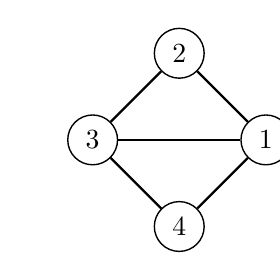
\begin{tikzpicture}
\GraphInit[vstyle=Normal]
\SetGraphUnit{1.1}
\Vertices{circle}{1,2,3,4}
\Edge(1)(2)
\Edge(1)(3)
\Edge(1)(4)
\Edge(2)(3)
\Edge(3)(4)
\end{tikzpicture}
\end{minipage}
\hspace*{0.5cm}
\begin{minipage}{4cm}
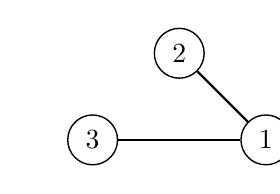
\begin{tikzpicture}
\GraphInit[vstyle=Normal]
\SetGraphUnit{1.1}
\Vertex{1}
\NOWE(1){2}
\SOWE(2){3}
\Edge(1)(2)
\Edge(1)(3)
\end{tikzpicture}
\end{minipage}
\hspace*{0.5cm}
\begin{minipage}{4cm}
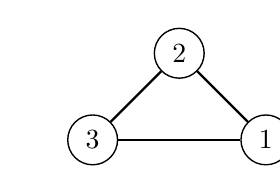
\begin{tikzpicture}
\GraphInit[vstyle=Normal]
\SetGraphUnit{1.1}
\Vertex{1}
\NOWE(1){2}
\SOWE(2){3}
\Edge(1)(2)
\Edge(1)(3)
\Edge(2)(3)
\end{tikzpicture}
\end{minipage}
\end{center}
\caption{A graph, a (non-induced) subgraph and an induced subgraph.}
\label{f:subgraph}
\end{figure}
If $G=(V,E)$ is a given graph (or digraph) and $U\subseteq V$, we
denote by $E[U]$ the subset of edges induced\index{induced} by $U$,
i.e.~the set of all edges in $E$ between vertices in $U$. Thus, if
$H=(U,F)$ is an induced subgraph of $G$, we can also denote $F$ by
$E[U]$. This notation is also extended to the whole subgraph: $H$ can
be denoted by $G[U]$.

\subsection{Stable and clique subgraphs}
\label{s:graph:subgraph:stable}
An induced subgraph\index{subgraph!induced} $H=(U,F)$ of $G$ is a
clique\index{clique} if it is complete,\index{complete} and a {\it
  stable}\index{stable} if it its edge set\index{edge!set} is
empty\index{empty} (see Fig.~\ref{f:cliquestab}).
\begin{figure}[!ht]
\begin{center}
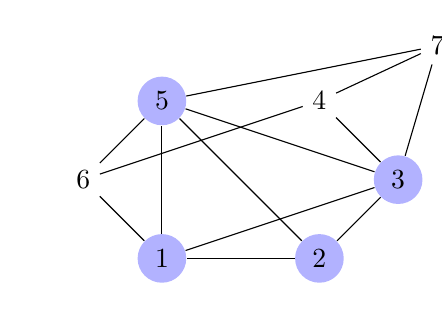
\begin{tikzpicture}[scale=1]
\node (v1) [circle,fill=blue!30] at (1,0) {$1$} ;
\node (v2) [circle,fill=blue!30] at (3,0) {$2$} ;
\node (v3) [circle,fill=blue!30] at (4,1) {$3$} ;
\node (v4) at (3,2) {$4$} ;
\node (v5) [circle,fill=blue!30] at (1,2) {$5$} ;
\node (v6) at (0,1) {$6$} ;
\node (v7) at (4.5,2.7) {$7$} ;
\draw (v1) to (v2) ;
\draw (v1) to (v3) ;
\draw (v1) to (v5) ;
\draw (v1) to (v6) ;
\draw (v2) to (v3) ;
\draw (v2) to (v5) ;
\draw (v3) to (v4) ;
\draw (v3) to (v5) ;
\draw (v3) to (v7) ;
\draw (v4) to (v6) ;
\draw (v4) to (v7) ;
\draw (v5) to (v6) ;
\draw (v5) to (v7) ;
\end{tikzpicture}
\hspace*{1cm}
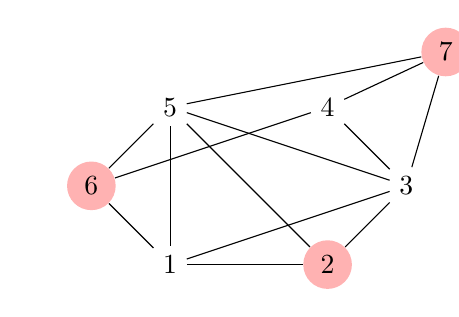
\begin{tikzpicture}[scale=1]
\node (v1) at (1,0) {$1$} ;
\node (v2) [circle,fill=red!30] at (3,0) {$2$} ;
\node (v3) at (4,1) {$3$} ;
\node (v4) at (3,2) {$4$} ;
\node (v5) at (1,2) {$5$} ;
\node (v6) [circle,fill=red!30] at (0,1) {$6$} ;
\node (v7) [circle,fill=red!30] at (4.5,2.7) {$7$} ;
\draw (v1) to (v2) ;
\draw (v1) to (v3) ;
\draw (v1) to (v5) ;
\draw (v1) to (v6) ;
\draw (v2) to (v3) ;
\draw (v2) to (v5) ;
\draw (v3) to (v4) ;
\draw (v3) to (v5) ;
\draw (v3) to (v7) ;
\draw (v4) to (v6) ;
\draw (v4) to (v7) ;
\draw (v5) to (v6) ;
\draw (v5) to (v7) ;
\end{tikzpicture}
\end{center}
\caption{A clique (left) and a stable (right) in $G$.}
\label{f:cliquestab}
\end{figure}
We also indicate stables by their vertex set\index{vertex!set} only,
since their edge set is empty, thus $U$ is a stable (or {\it stable
  set},\index{stable!set} or {\it independent
  set})\index{independent!set} if $G[U]$ is a stable.

\subsection{Some applications}
Many combinatorial problems consist of looking for a subgraph (be it
induced or not) of a given graph with certain properties. The {\sc
  Subgraph Isomorphism Problem}\index{subgraph!isomorphism} (SIP), for
example, is as follows. Given two graphs $G,H$, does $G$ contain a
subgraph which is isomorphic to $H$ (see Fig.~\ref{f:sip})? The SIP
has applications in mining molecule\index{molecule} databases,
e.g.~when trying to determine whether a given protein\index{protein}
has a side-chain\index{side-chain} with a particular shape but
possibly different atoms.\index{atom}
\begin{figure}[!ht]
\begin{center}
\begin{minipage}{4cm}
$G$
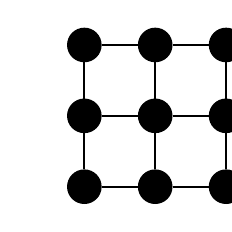
\begin{tikzpicture}
\GraphInit[vstyle=Classic]
\SetGraphUnit{0.9}
\SetVertexNoLabel
\Vertex{1}
\EA(1){2}
\NOEA(1){3}
\NO(1){4}
\NOWE(1){5}
\WE(1){6}
\SOWE(1){7}
\SO(1){8}
\SOEA(1){9}
\Edge(1)(2)
\Edge(2)(3)
\Edge(3)(4)
\Edge(1)(4)
\Edge(4)(5)
\Edge(5)(6)
\Edge(1)(6)
\Edge(6)(7)
\Edge(7)(8)
\Edge(1)(8)
\Edge(8)(9)
\Edge(2)(9)
\end{tikzpicture}
\end{minipage}
\hspace*{0.5cm}
\begin{minipage}{4cm}
$H$
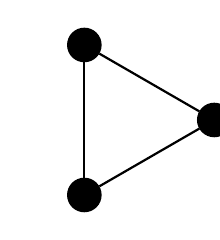
\begin{tikzpicture}
\GraphInit[vstyle=Classic]
\SetGraphUnit{1.1}
\SetVertexNoLabel
\Vertices{circle}{1,2,3}
\Edges(1,2,3,1)
\end{tikzpicture}
\end{minipage}
\hspace*{0.5cm}
\begin{minipage}{4cm}
$K$
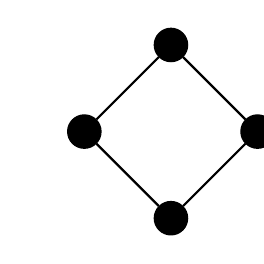
\begin{tikzpicture}
\GraphInit[vstyle=Classic]
\SetGraphUnit{1.1}
\SetVertexNoLabel
\Vertices{circle}{1,2,3,4}
\Edges(1,2,3,4,1)
\end{tikzpicture}
\end{minipage}
\end{center}
\caption{$H$ is isomorphic to no subgraph of $G$, but $K$ obviously is.}
\label{f:sip}
\end{figure}

The {\sc Densest Subgraph Problem}\index{subgraph!densest} (DSP) looks
for a subgraph of maximum density in a given graph (see
Fig.~\ref{f:dsp}); the density of a graph $G=(V,E)$ is defined as
$\frac{|E|}{|V|}$. The DSP has applications in clustering.
\begin{figure}[!ht]
\begin{center}
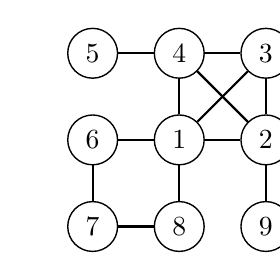
\begin{tikzpicture}
\GraphInit[vstyle=Normal]
\SetGraphUnit{1.1}
\Vertex{1}
\EA(1){2}
\NOEA(1){3}
\NO(1){4}
\NOWE(1){5}
\WE(1){6}
\SOWE(1){7}
\SO(1){8}
\SOEA(1){9}
\Edge(1)(2)
\Edge(1)(3)
\Edge(2)(4)
\Edge(2)(3)
\Edge(3)(4)
\Edge(1)(4)
\Edge(4)(5)
%\Edge(5)(6)
\Edge(1)(6)
\Edge(6)(7)
\Edge(7)(8)
\Edge(1)(8)
%\Edge(8)(9)
\Edge(2)(9)
\end{tikzpicture}
\end{center}
\caption{The densest subgraph of this graph is induced by $\{1,2,3,4\}
$.}
\label{f:dsp}
\end{figure}

\section{Connectivity}
\label{s:graph:connected}
We can extend the concept of neighbourhood to sets of vertices: let
$G=(V,E)$ be a graph, and $U\subseteq V$. Then the neighbourhood of
$U$ in $G$ is 
\begin{equation*}
  N_G(U)=\bigcup\limits_{u\in U} N_G(u)\smallsetminus U, 
\end{equation*}
i.e.~the set of vertices in $V\smallsetminus U$ adjacent to vertices
in $U$.  The {\it cutset}\index{cutset} of $U$ in $G$ is
\begin{equation*}
  \delta_G(U)=\bigcup\limits_{u\in U}\delta_G(u)\smallsetminus E[U],
\end{equation*}
i.e.~the set of edges adjacent to exactly one vertex in $U$.
A cutset is {\it trivial}\index{cutset!trivial} if $U=\varnothing$ or
$U=V$.  These definitions all extend to the case of digraph in a
natural way. Cutsets allow us to explain connectivity in purely
topological terms: a graph $G=(V,E)$ is {\it
  connected}\index{connected}\index{graph!connected} if no nontrivial
cutset is empty (see Fig.~\ref{f:connected}).
\begin{figure}[!ht]
\begin{center}
\begin{minipage}{5cm}
$G$
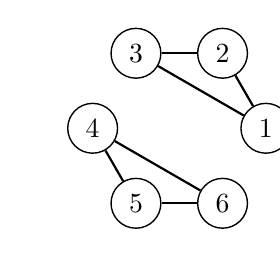
\begin{tikzpicture}
\GraphInit[vstyle=Normal]
\SetGraphUnit{1.1}
\Vertices{circle}{1,2,3,4,5,6}
\Edges(1,2,3,1)
\Edges(4,5,6,4)
\end{tikzpicture}
\end{minipage}
\hspace*{1cm}
\begin{minipage}{5cm}
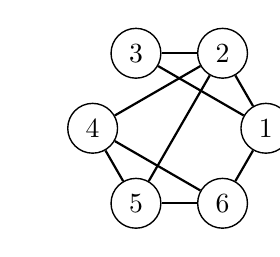
\begin{tikzpicture}
\GraphInit[vstyle=Normal]
\SetGraphUnit{1.1}
\Vertices{circle}{1,2,3,4,5,6}
\Edge(2)(5)
\Edge(2)(4)
\Edge(1)(6)
\Edges(1,2,3,1)
\Edges(4,5,6,4)
\end{tikzpicture}
$H$
\end{minipage}
\end{center}
\caption{$G$ is not connected: the cutset defined by $\{1,2,3\}$ is
  nontrivial and empty; $H$, on the other hand, is connected.}
\label{f:connected}
\end{figure}

A digraph is connected if its underlying graph is; however, this
notion of connectivity is not often used for digraphs. The appropriate
connectivity notion in digraphs is called ``strong
connectivity''\index{graph!strongly connected} and will be discussed
later.

The concept of connectivity arises in networks. In power networks, for
example, blackouts may arise in large geographical areas when a part
of the network is disconnected. Power networks are robust to such
events when all cutsets have large cardinality.

\subsection{Simple paths}
A graph $G=(V,E)$ is a {\it simple path}\index{path!simple} if is it
connected and each vertex has degree\index{degree} at most 2 (see
Fig.~\ref{f:path}).
\begin{figure}[!ht]
\begin{center}
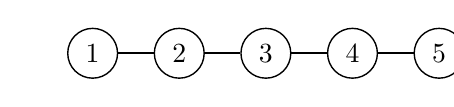
\begin{tikzpicture}
\GraphInit[vstyle=Normal]
\SetGraphUnit{1.1}
\Vertex{1}
\EA(1){2}
\EA(2){3}
\EA(3){4}
\EA(4){5}
\Edges(1,2,3,4,5)
\end{tikzpicture}
\end{center}
\caption{A simple path. Vertices 1,5 have unit degrees, while 2,3,4 have
  degree two.}
\label{f:path}
\end{figure}

Paths have multiple applications in any number of engineering,
scientific and even mathematical problems. Shortest paths are often
used in routing materials in transportation networks; robust paths are
used in communication or power networks. The {\sc Shortest Path
  Problem}\index{shortest path problem@{\sc Shortest Path Problem}}
(SPP)\index{SPP} (see Chapter \ref{c:path}) often arises as a
sub-problem in more complicated problems.

\subsection{An alternative definition of paths and connectivity}
Most textbooks on graph theory introduce paths before connectivity,
defining the latter in terms of the former: a path\index{path} with
endpoints\index{path!endpoint} $v_1,v_n$ is a graph $G=(V,E)$, where
$V$ is ordered as $(v_1,v_2,\ldots,v_n)$, such that for all $i<n$,
$\{v_i,v_{i+1}\}\in E$. Moreover, a graph $H$ is connected if for all
$u\not=v$ in $V(H)$ there is a path in $H$ with endpoints $u,v$. This,
however, requires the concept of {\it order}\index{order} to be used
to introduce connectivity. Employing cutsets defines connectivity in a
purely graph-theoretical way.
\begin{ex}
Prove that the two definitions of graph connectivity are equivalent.
\end{ex}

\subsection{Paths: not so simple}
In the previous sections we defined ``simple
paths''\index{path!simple} as well as ``paths''\index{path}. What is
the difference? A simple path is certainly a path (prove this), but
the converse may not hold. Consider the path
$(v_1,v_2,v_3,v_4,v_5,v_3)$ shown in Fig.~\ref{f:path2}.
\begin{figure}[!ht]
\begin{center}
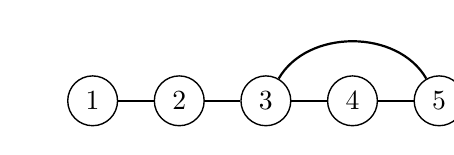
\begin{tikzpicture}
\GraphInit[vstyle=Normal]
\SetGraphUnit{1.1}
\Vertices{line}{1,2,3,4,5}
\Edges(1,2,3,4,5)
\tikzset{EdgeStyle/.style = {-,bend right=60}}
\Edge(5)(3)
\end{tikzpicture}
\end{center}
\caption{A non-simple path.}
\label{f:path2}
\end{figure}
This graph is certainly a path, since it is defined by the order
$v_1,v_2,v_3,v_4,v_5,v_3$, but since $v_3$ is repeated in the order,
the path fails to be simple, as vertex 3 has degree three. In general,
paths that ``cross themselves'' or have loops or traverse edges more
than once (thus yielding a multigraph --- can you see why this is so?)
are not simple. Paths are also known as {\it walks}\index{walk}, or
{\it trails}\index{trail} if all traversed edges are distinct.

\subsection{Strong connectivity}
Walks (or trails) can be easily adapted to the case of digraphs: in
this setting, a walk\index{walk} is an alternating sequence of nodes
and arcs, beginning and ending with a node. A digraph $G$ is {\it
  strongly connected}\index{digraph!strongly connected}\index{strongly
  connected} if for each ordered pair $(u,v)$ of distinct nodes of
$V(G)$ there is a walk in $G$ starting at $u$ and ending at $v$ (see
Fig.~\ref{f:strongc}).
\begin{figure}[!ht]
\begin{center}
\begin{minipage}{5cm}
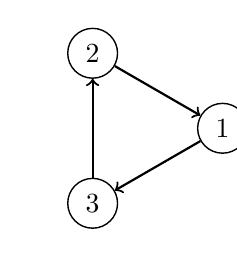
\begin{tikzpicture}
\GraphInit[vstyle=Normal]
\SetGraphUnit{1.1}
\Vertices{circle}{1,2,3}
\tikzset{EdgeStyle/.style = {->}}
\Edges(1,3,2,1)
\end{tikzpicture}
\end{minipage}
\hspace*{1cm}
\begin{minipage}{5cm}
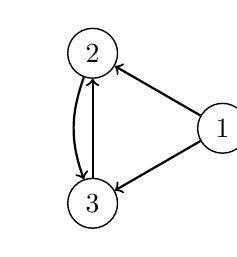
\begin{tikzpicture}
\GraphInit[vstyle=Normal]
\SetGraphUnit{1.1}
\Vertices{circle}{1,2,3}
\tikzset{EdgeStyle/.style = {->}}
\Edges(1,3,2)
\Edge(1)(2)
\tikzset{EdgeStyle/.style = {->,bend right=20}}
\Edge(2)(3)
\end{tikzpicture}
\end{minipage}
\end{center}
\caption{On the left, a strongly connected digraph. The graph on the
  right is not strongly connected, as there is no walk from vertex 3
  to vertex 1.}
\label{f:strongc}
\end{figure}

\subsection{Cycles}
A {\it simple cycle}\index{cycle!simple} in a graph is a path where
all vertices have degree 2. A {\it cycle} in a graph is a subgraph
where all vertices have even degree (see Fig.~\ref{f:cycle}).
\begin{figure}[!ht]
\begin{center}
\begin{minipage}{4cm}
$G$
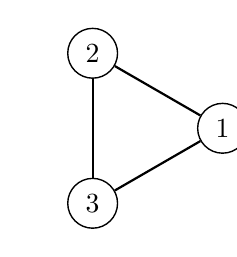
\begin{tikzpicture}
\GraphInit[vstyle=Normal]
\SetGraphUnit{1.1}
\Vertices{circle}{1,2,3}
\Edges(1,2,3,1)
\end{tikzpicture}
\end{minipage}
\hspace*{0.5cm}
\begin{minipage}{4cm}
$H$
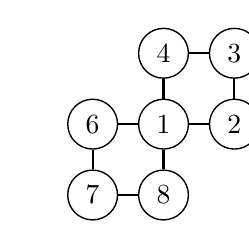
\begin{tikzpicture}
\GraphInit[vstyle=Normal]
\SetGraphUnit{0.9}
\Vertex{1}
\EA(1){2}
\NOEA(1){3}
\NO(1){4}
\WE(1){6}
\SOWE(1){7}
\SO(1){8}
\Edge(1)(2)
\Edge(2)(3)
\Edge(3)(4)
\Edge(1)(4)
\Edge(1)(6)
\Edge(6)(7)
\Edge(7)(8)
\Edge(1)(8)
\end{tikzpicture}
\end{minipage}
\hspace*{0.5cm}
\begin{minipage}{4cm}
$K$
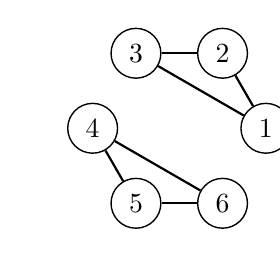
\begin{tikzpicture}
\GraphInit[vstyle=Normal]
\SetGraphUnit{1.1}
\Vertices{circle}{1,2,3,4,5,6}
\Edges(1,2,3,1)
\Edges(4,5,6,4)
\end{tikzpicture}
\end{minipage}
\end{center}
\caption{$G$ is a simple cycle, $H,K$ are cycles that are not simple.}
\label{f:cycle}
\end{figure}

Computations concerning cycles in graphs often arise as sub-steps of
certain graph-related algorithms (see
e.g.~Sect.~\ref{s:path:negcycle}). Cycles are often used as a proof
that networks are robust to failures: if two nodes $u,v$ of a network
are involved in a cycle, then there must be two different paths from
$u$ to $v$: in case one fails, the other provides connectivity.

\subsection{An alternative definition of cycles}
\label{s:graph:altcycle}
Again, most graph theory textbooks define cycles in a different way,
notably as {\it closed walks},\index{walk!closed} which are walks
whose endpoints coincide (e.g.~$G,H$ in Fig.~\ref{f:cycle} are closed
walks). Moreover, if the walk is a trail,\index{trail} i.e.~no edge is
traversed more than once, then the corresponding closed trail is
called a {\it tour}\index{tour} or {\it circuit}.\index{circuit} These
definitions would prevent the graph $K$ in Fig.~\ref{f:cycle} to be
called ``cycle'', evidently, as it is not connected, whereas any walk
or trail is connected by definition. And, to be fair, intuitively
speaking the graph $K$ looks like {\it two} cycles rather than just
one. We justify our choice below.

\subsection{The cycle space}
\label{s:graph:cyclespace}
We have two reasons for defining a cycle as a subgraph of even
degree. The first is its simplicity. The second is that, under this
definition, the set $\mathcal{C}(G)$ of all cycles of a graph forms a
vector space $(\mathcal{C}(G),\oplus)$ over the finite field
$\mathbb{F}_2=\{0,1\}$, called the {\it cycle
  space}.\index{cycle!space} The rules for adding two cycles in this
vector space can be deduced from the following examples.
\begin{eqnarray}
\begin{minipage}{2cm}
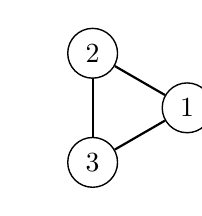
\begin{tikzpicture}
\GraphInit[vstyle=Normal]
\SetGraphUnit{0.8}
\Vertices{circle}{1,2,3}
\Edges(1,2,3,1)
\end{tikzpicture}
\end{minipage}
\oplus
\begin{minipage}{2cm}
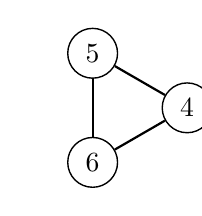
\begin{tikzpicture}
\GraphInit[vstyle=Normal]
\SetGraphUnit{0.8}
\Vertices{circle}{4,5,6}
%\Edges(1,2,3,1)
\Edges(4,5,6,4)
\end{tikzpicture}
\end{minipage}
&=&
\begin{minipage}{3cm}
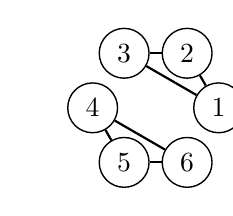
\begin{tikzpicture}
\GraphInit[vstyle=Normal]
\SetGraphUnit{0.8}
\Vertices{circle}{1,2,3,4,5,6}
\Edges(1,2,3,1)
\Edges(4,5,6,4)
\end{tikzpicture}
\end{minipage}
\label{eq:cycle1}
\\
\begin{minipage}{2cm}
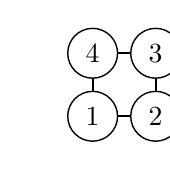
\begin{tikzpicture}
\GraphInit[vstyle=Normal]
\SetGraphUnit{0.8}
\Vertex{1}
\EA(1){2}
\NOEA(1){3}
\NO(1){4}
%\WE(1){6}
%\SOWE(1){7}
%\SO(1){8}
\Edge(1)(2)
\Edge(2)(3)
\Edge(3)(4)
\Edge(1)(4)
%\Edge(1)(6)
%\Edge(6)(7)
%\Edge(7)(8)
%\Edge(1)(8)
\end{tikzpicture}
\end{minipage}
\oplus
\begin{minipage}{2cm}
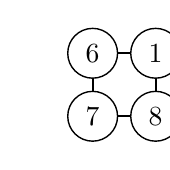
\begin{tikzpicture}
\GraphInit[vstyle=Normal]
\SetGraphUnit{0.8}
\Vertex{1}
%\EA(1){2}
%\NOEA(1){3}
%\NO(1){4}
\WE(1){6}
\SOWE(1){7}
\SO(1){8}
%\Edge(1)(2)
%\Edge(2)(3)
%\Edge(3)(4)
%\Edge(1)(4)
\Edge(1)(6)
\Edge(6)(7)
\Edge(7)(8)
\Edge(1)(8)
\end{tikzpicture}
\end{minipage}
&=&
\begin{minipage}{3cm}
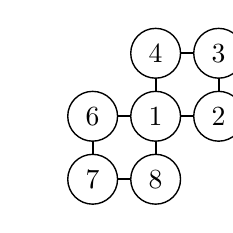
\begin{tikzpicture}
\GraphInit[vstyle=Normal]
\SetGraphUnit{0.8}
\Vertex{1}
\EA(1){2}
\NOEA(1){3}
\NO(1){4}
\WE(1){6}
\SOWE(1){7}
\SO(1){8}
\Edge(1)(2)
\Edge(2)(3)
\Edge(3)(4)
\Edge(1)(4)
\Edge(1)(6)
\Edge(6)(7)
\Edge(7)(8)
\Edge(1)(8)
\end{tikzpicture}
\end{minipage}
\label{eq:cycle2}
\\
\begin{minipage}{2cm}
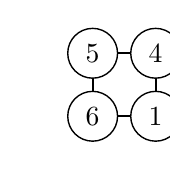
\begin{tikzpicture}
\GraphInit[vstyle=Normal]
\SetGraphUnit{0.8}
\Vertex{1}
%\EA(1){2}
%\NOEA(1){3}
\NO(1){4}
\NOWE(1){5}
\WE(1){6}
%\Edge(1)(2)
%\Edge(2)(3)
%\Edge(3)(4)
\Edge(1)(4)
\Edge(4)(5)
\Edge(5)(6)
\Edge(1)(6)
\end{tikzpicture}
\end{minipage}
\oplus
\begin{minipage}{2cm}
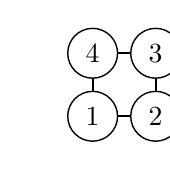
\begin{tikzpicture}
\GraphInit[vstyle=Normal]
\SetGraphUnit{0.8}
\Vertex{1}
\EA(1){2}
\NOEA(1){3}
\NO(1){4}
%\NOWE(1){5}
%\WE(1){6}
\Edge(1)(2)
\Edge(2)(3)
\Edge(3)(4)
\Edge(1)(4)
%\Edge(4)(5)
%\Edge(5)(6)
%\Edge(1)(6)
\end{tikzpicture}
\end{minipage}
&=&
\begin{minipage}{3cm}
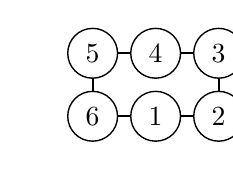
\begin{tikzpicture}
\GraphInit[vstyle=Normal]
\SetGraphUnit{0.8}
\Vertex{1}
\EA(1){2}
\NOEA(1){3}
\NO(1){4}
\NOWE(1){5}
\WE(1){6}
\Edge(1)(2)
\Edge(2)(3)
\Edge(3)(4)
%\Edge(1)(4)
\Edge(4)(5)
\Edge(5)(6)
\Edge(1)(6)
\end{tikzpicture}
\end{minipage}
\label{eq:cycle3}
\end{eqnarray}
More precisely, let $\gamma_1,\gamma_2$ be two cycles in the graph
$G$. If $V(\gamma_1)\cap V(\gamma_2)=\varnothing$, i.e.~the two cycles
have no common vertex (and hence no common edge either --- why?), then
the resulting cycle is simply the union of the two graphs $\gamma_1$
and $\gamma_2$, as shown in Eq.~\eqref{eq:cycle1}. If
$\gamma_1,\gamma_2$ have a common vertex, again the resulting cycle is
the union of $\gamma_1,\gamma_2$, as shown in
Eq.~\eqref{eq:cycle2}. If the intersection of $\gamma_1,\gamma_2$
contains some edges, then the resulting cycle will contain edges in
$\gamma_1$ or $\gamma_2$ but not both:
\begin{equation*}
  E(\gamma_1\oplus\gamma_2)=E(\gamma_1)\triangle E(\gamma_2)=
    (E(\gamma_1)\cup E(\gamma_2))\smallsetminus (E(\gamma_1)\cap
  E(\gamma_2)).
\end{equation*}

Like any vector space, the cycle space has a dimension and bases. We
state the next result without proof (see e.g.~\cite{seshu} for a
proof).
\begin{thm}
The cycle space has dimension $|E|-|V|+1$.
\label{thm:cycspdim}
\end{thm}
Bases of the cycle space allow a compact (linear) description of the
(exponentially large) cycle space of a graph --- this comes in handy
in the classification of ring compounds in molecular chemistry, in the
analysis and simulation of electrical circuits, and in the synthesis
of public transportation timetables. Although extensions of these
concepts to digraphs exist in the graph theory literature, they are
are not sufficiently mainstream to introduce them in this
course. 

\subsubsection{Cycle-edge incidence vectors}
The {\it cycle-edge incidence
  vector}\index{vector!incidence!cycle-edge} of a cycle $\gamma$ is a
binary vector\index{vector!binary} with $m=|E|$ columns, that has a 1
in component $e\in E$ if and only if $e$ is an edge in $\gamma$. For a
cycle $\gamma$, let $\inc({\gamma})$ be the incidence
vector\index{vector!incidence} of $\gamma$. We define a XOR\index{XOR}
operation on two binary vectors $\vec{u},\vec{v}$ of the same length
as follows: for any component index $i$, the $i$-th component of
$\vec{u}\,\mbox{XOR}\,\vec{v}$ is $\vec{u}_i\,\mbox{XOR}\,\vec{v}_i$.
\begin{ex}
For any two cycles $\gamma,\gamma'$ of the same graph $G$, prove that
$\inc(\gamma\oplus\gamma')=\inc(\gamma)\,\mbox{XOR}\,\inc(\gamma')$. 
\end{ex}

\section{Basic operations on graphs}
\label{s:graph:operation}
In later chapters, we are going to employ graphs to discuss some data
structures. We are going to need mechanisms for modifying graphs as a
result of the CPU modifying the data and the relations between
data. 

\subsection{Addition and removal of vertices and edges}
\label{s:graph:operation:addrem}
The easiest operations on a graph\index{graph!operation} $G=(V,E)$ are
the addition\index{vertex!addition}\index{vertex!removal} and removal
of vertices and edges.\index{edge!addition}\index{edge!removal} We
suppose that $V\subseteq\mathbb{N}$. To add a vertex to $V$, we pick
an integer $v$ which is not already in $V$ and we set $V\leftarrow
V\cup\{v\}$. To add an edge $\{u,v\}$ to $E$, we first verify whether
$\{u,v\}$ is already in $E$ or not. If it is, then we increase its
multiplicity by one, obtaining a multigraph. Otherwise, we set
$E\leftarrow E\cup\{\{u,v\}\}$.

To remove an edge $\{u,v\}\in E$ from $E$, we simply set $E\leftarrow
E\smallsetminus\{\{u,v\}\}$. Removing a vertex $v$ from $V$ is
slightly more involved, as we have to remove $v$ and all edges
incident to $v$:
\begin{eqnarray*}
  V &\leftarrow& V\smallsetminus \{v\} \\
  E &\leftarrow& E\smallsetminus \delta(v).
\end{eqnarray*}

\begin{eg}
\vspace*{1em}
To turn the graph 
\begin{minipage}{1.5cm}
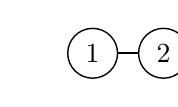
\begin{tikzpicture}
\GraphInit[vstyle=Normal]
\SetGraphUnit{0.9}
\Vertices{line}{1,2}
\Edge(1)(2)
\end{tikzpicture}
\end{minipage}
into the graph
\begin{minipage}{2.5cm}
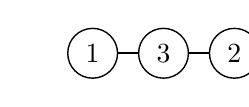
\begin{tikzpicture}
\GraphInit[vstyle=Normal]
\SetGraphUnit{0.9}
\Vertices{line}{1,3,2}
\Edges(1,3,2)
\end{tikzpicture}
\end{minipage},
perform the following operations:
\begin{enumerate}
\item add vertex $3$
\item add edges $\{1,3\}$, $\{2,3\}$
\item remove edge $\{1,2\}$.
\end{enumerate}
Conversely, to turn the latter into the former:
\begin{enumerate}
\item remove vertex $3$
\item add edge $\{1,2\}$.
\end{enumerate}
\end{eg}

\subsection{Contraction}
Contracting\index{contraction} an edge\index{edge!contraction}
$\{u,v\}\in E$ essentially means ``replace an edge with a
vertex''. More precisely, it consists of the following basic steps
(see Fig.~\ref{f:edgecontract}):
\begin{enumerate}
\item add a vertex $z$
\item for each $w\in N(u)\cup N(v)$ add the edge $\{w,z\}$
\item remove the vertices $u$ and $v$.
\end{enumerate}
\begin{figure}[!ht]
\begin{center}
\psfrag{u}{$u$}
\psfrag{v}{$v$}
\psfrag{z}{$z$}
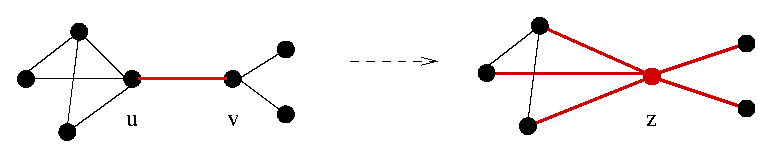
\includegraphics[width=7cm]{edgecontract}
\end{center}
\caption{Edge contraction operation.}
\label{f:edgecontract}
\end{figure}
Contracting a whole subgraph\index{subgraph!contraction} $H$ in a
graph $G$ means contracting each edge in $E(H)$ to the same vertex
$v_H$ (Fig.~\ref{f:subgraphcontract}).
\begin{figure}[!ht]
\begin{center}
\psfrag{H}{$H$}
\psfrag{vH}{$v_H$}
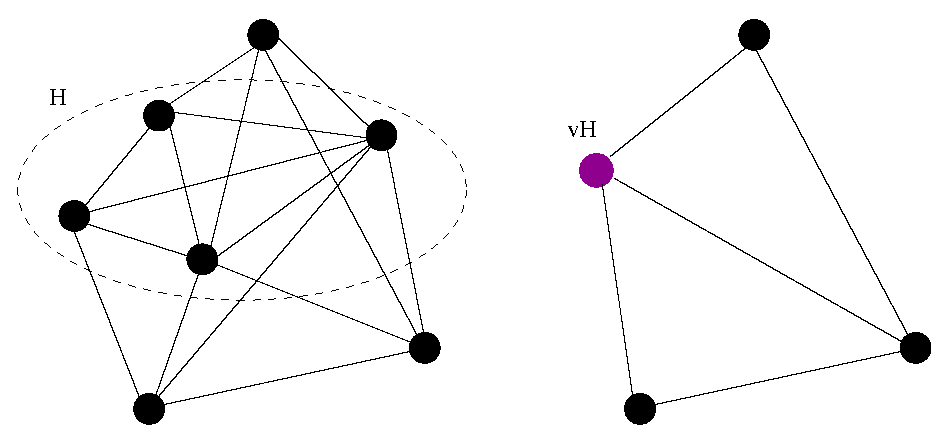
\includegraphics[width=8cm]{contraction}
\end{center}
\caption{Subgraph contraction operation.}
\label{f:subgraphcontract}
\end{figure}
Contracting an unlabeled subgraph $H$ is a way to look at a complex
graph ``modulo $H$''; intuitively, it looks like zooming out of a
complicated-looking graph to try and ascertain the core topological
characteristics (Fig.~\ref{f:networkcontract}).
\begin{figure}[!ht]
\begin{center}
\includegraphics[width=12cm]{networkcontraction}
\end{center}
\caption{Contraction: zooming out of a complicated graph.}
\label{f:networkcontract}
\end{figure}
The graph $G'$ obtained from $G$ through a sequence of contractions is
called a {\it minor}\index{graph!minor}\index{minor} of $G$. 

%%%%%%%%%%%%%%%%% CHAPTER: LINEAR DATA STRUCTURES %%%%%%%%%%%%%%%%%%%%

\chapter{Linear data structures}
\label{c:linear}

\begin{center}
\fbox{\begin{minipage}{13cm}{\small {\sc Abstract}.  
Arrays: jagged arrays and adjacency lists, array operations,
worst-case and average complexity of an incomplete loop. Lists and
list operations, with a Java implementation. Queues, implemented as
circular arrays. Stacks, with an example and an implementation. Maps.
Use of parametrized classes. 
}
\end{minipage}}
\end{center}

We saw how data can be structured\index{data!structure} according to a
class\index{class} description, and also how arrays\index{array} can
contain several objects\index{object} of the same class. In this
context, arrays are one of many existing types of {\it data
  structures}\index{data!structure} (or {\it data
  containers}).\index{data!container} The objects held in a data
structure, such as an array, list, queue, tree or other, are called
{\it entries},\index{data!structure!entry} or {\it
  elements}.\index{data!structure!element}

\section{Arrays}
\label{s:linear:array}
Arrays\index{array} were introduced in
Sect.~\ref{s:java:array}. Arrays implement a vector\index{vector}, 
a matrix\index{matrix} or a tensor\index{tensor} in mathematics. They
model a contiguous, possibly
multi-dimensional\index{array!multidimensional} block of
memory.\index{memory!block} Accordingly, we shall represent a linear
array\index{array!linear} as a vector $x=(x_0,\ldots,x_{n-1})$, where
$n$ is the size of the array; for multi-dimensional arrays, each
element $x_i$ might itself be an array. This nesting is repeated as
many times as the array has dimensions. The memory allocated to the
array must be enough to hold at least $n$ objects. Normally, the
memory size does not change throughout the program, which implies that
there is a limit to the number of objects we can insert into an
array. Bypassing this limit is technically possible, but it involves
resizing the array, which is an expensive operation in terms of CPU time.

We remark that {\bf indexing\index{index} starts from
  zero}\footnote{In later chapters, when we pass from a code-oriented
  practical approach to a more theoretical setting, we shall employ
  arrays without necessarily assuming they are indexed starting from
  zero.} in Java,\index{Java} C\index{C} and C++.\index{C++} The fact
that the array elements are contiguous makes memory
access\index{memory!access} very efficient. Reading or writing the
$i$-th element of the array, given the memory address for $x[0]$,
simply requires adding $i\times$ (length of the stored objects) bytes
to it. This type of {\it index arithmetic}\index{index!arithmetic} is
carried out automatically by the Java compiler.\index{compiler}

\subsection{Jagged arrays}
\label{s:linear:array:jagged}
A {\it jagged array}\index{array!jagged} is simply a multi-dimensional
array in its most general configuration, i.e.~where sub-arrays might
have different sizes (see Fig.~\ref{f:jaggedarray}).
\begin{figure}[!ht]
\begin{center}
\begin{tabular}{cl}
$x$ & \\
\fbox{$x_0$} & \fbox{$x_{00}$}\fbox{$x_{01}$} \\
\fbox{$x_1$} & \fbox{$x_{10}$}\fbox{$x_{11}$}\fbox{$x_{12}$}
\end{tabular}
\end{center}
\caption{A jagged array structure.}
\label{f:jaggedarray}
\end{figure}

\subsubsection{Adjacency lists}
\label{s:linear:array:jagged:adjacencylist}
Jagged arrays are useful to represent a graph\index{graph} $G=(V,E)$:
rows\index{row} are indexed by $v\in V$, and each row contains the elements of
the star\index{star} $\delta(v)$ in some order, arbitrary or
otherwise. The generalization to digraphs\index{digraph} is easy: each
row only contains $\delta^+(v)$ or $\delta^-(v)$ depending on the
context (we might even store both incoming and outgoing
stars\index{star!incoming}\index{star!outgoing} if need be). 

\begin{eg} Let $V=\{1,2,3\}$ and 
  $E=\{(1,1),(1,2),(2,3),(3,1),(3,2),(3,3)\}$; the corresponding
  digraph can be represented in memory by means of a jagged array
  structure as follows.
\begin{equation*}
\begin{array}{|c|ccc} \hline
1 & 1 & 2 & \\ \hline
2 & 3 &   & \\ \hline
3 & 1 & 2 & 3 \\ \hline
\end{array}
\end{equation*}
\end{eg}

This graph representation is called {\it adjacency
  list}.\index{list!adjacency}\index{graph!adjacency list} Another
common graph representation\index{graph!representation} is by an edge
array, or edge list\index{list!edge}\index{graph!edge list} (arc array
or list\index{list!arc}\index{digraph!arc list} in the case of
digraphs).\index{digraph} The two representations are useful in
different contexts.

\subsection{Array operations}
\label{s:array:operations}
The usual operations\index{array!operations} an array can carry out on
the objects it stores are:
\begin{itemize}
\item read\index{array!read}\index{read!array} the value of the $i$-th
  component (worst-case complexity\index{complexity!array} $O(1)$)
\item write\index{array!write}\index{write!array} the value of the
  $i$-th component (worst-case complexity\index{array!complexity}
  $O(1)$)
\item return the size\index{array!size}\index{size!array} $n$ of the
  array (worst-case complexity $O(n)$ or $O(1)$, depending on the
  implementation\footnote{With a Java array {\tt a}, {\tt a.length}
    returns its size in $O(1)$.})
\item remove\index{array!remove}\index{remove!array} the $i$-th
  element (worst-case complexity $O(n)$)
\item insert\index{array!insert}\index{insert!array} an element at the
  $i$-th position (worst-case complexity $O(n)$)
\item move\index{array!move}\index{move!array} a subsequence
  (contiguous set) of entries just after position $i$ (worst-case
  complexity $O(n)$).
\end{itemize}
In summary, arrays are efficient\index{array!efficiency} when a lot of
read/write accesses are needed at random\index{random access}
positions, and the positions of the entries does not change.

\begin{ex}
Show how the read and write array operations can be implemented in
$O(1)$.
\end{ex}

\subsubsection{Size in $O(1)$}
The {\it array size}\index{array!size} is defined as the number of
elements of the array, which is at most the amount of memory required
to hold them: we call the latter quantity {\it array memory
  size}.\index{array!memory size} The array memory size can be
returned by asking the operating system\index{operating system} how
much memory was allocated starting to a given address.

In order to determine the array size, some array implementations
employ a {\it delimiter}\index{delimiter}\index{array!delimiter},
stored as a ``special character'' (such as the ASCII 0 code) at the
array element after the last. Finding the size can then be an $O(n)$
operation: starting with $i=0$, increase $i$ until $x_i$ becomes the
delimiter value, as in the pseudocode below.
\begin{algorithmic}
  \STATE $i\leftarrow 0$;
  \WHILE{$x_i\not=\mbox{delimiter}$}
    \STATE $i\leftarrow i+1$;
  \ENDWHILE
  \STATE $n\leftarrow i+1$;
  \RETURN $n$
\end{algorithmic}

This can be improved to $O(1)$ if we simply store the array size
within the array itself. An array of integers could then be conceived
as an object of the following class:
\begin{verbatim}
class Array {
  public int size;
  public int[] theArray;
}
\end{verbatim}
Any array operation changing the size must then update the {\tt size}
attribute accordingly. Asking for the size then becomes a simple
matter of returning {\tt size}, which is an $O(1)$ operation.

We remark that Java's standard array implementation is already $O(1)$,
without you needing to re-code a new array structure with this
property. This section is simply meant to tell you that this is not a
trivial array property. 

\subsubsection{Moving a subsequence}
\label{s:linear:array:splice}
Let $x$ be a given array of size $n$, $i\in\{0,\ldots,n-1\}$, and
$L=(x_\ell,\ldots,x_{\ell+h})$ be the subsequence\index{subsequence}
we want to move to the position right after $i$. This can be attained
by means of $h$ swaps. A {\it swap}\index{memory!swap}\index{swap}
$(j,k)$ consists in the following instructions:
\begin{enumerate}
\item store the value $x_j$ in a temporary
  variable\index{variable!temporary} $t$
\item copy the value $x_k$ in the array entry\index{array!entry}
  indexed by $j$
\item copy the value of $t$ in the array entry indexed by $k$.
\end{enumerate}
After the swap $(j,k)$, the effect on $x$ is that $x_j$ and $x_k$ have
swapped their values. 

The following pseudocode moves the subsequence\index{subsequence} $L$
to the position $i+1$ in $x$ (as long as $i<\ell$ or $i>\ell+h$),
automatically re-positioning the elements that are currently stored at
position $i+1$ and following (see Fig.~\ref{f:splice}).
\begin{algorithmic}
\FOR{$j\in\{0,\ldots,h\}$}
  \STATE swap $(\ell+j,i+j+1)$  
\ENDFOR
\end{algorithmic}
This operation, which is also called {\it splice}\index{array!splice},
has worst-case complexity $O(n)$. The worst case occurs when the
subsequence $(x_2,\ldots,x_n)$ must be moved to position 1.
\begin{figure}[!ht]
\begin{center}
\psfrag{i}{$i$}
\psfrag{L1}{$x_\ell$}
\psfrag{L2}{$\!\!x_{\ell+1}$}
\includegraphics[width=14cm]{splice}
\end{center}
\caption{Array splicing.}
\label{f:splice}
\end{figure}

\begin{ex}
Adapt the splicing algorithm to all $i$, removing the assumption that
$i<\ell$ or $i>\ell+h$.
\end{ex}

\subsubsection{Removal and insertion}
Both removal\index{array!removal} and insertion\index{array!insertion}
operations can be carried out by splicing the array (see
Sect.~\ref{s:linear:array:splice}). To remove element $x_i$, we move
$(x_{i+1},\ldots,x_n)$ to position $i$ (so that $x_{i+1}$ overwrites
$x_i$, and so on). To insert a new element $a$ at position $i$, we
move $(x_i,\ldots,x_n)$ to position $i+1$ (this is only possible if
memory enough to hold $n+1$ objects was initially allocated to $x$),
then set $x_i=a$. 

\begin{ex}
Show that both removal and insertion have $O(n)$ worst-case
complexity.
\end{ex}

\subsection{Complexity of an incomplete loop}
\label{s:linear:array:incomplete}
In Sect.~\ref{s:computation:timeworstcase} we analyzed the worst-case
complexity of a simple loop,\index{loop!simple} i.e.~a loop where the
termination condition is constant over the whole loop execution. Here
we analyze the average-case complexity\index{complexity!average-case}
of a specific instance of a non-simple loop.\index{loop} Consider the
following loop.
\begin{algorithmic}[1]
\STATE input $x\in\{0,1\}^n$; \label{step:input}
\STATE $\mbox{\tt int }i=0$;
\WHILE{$(i<n \land x_i=1)$}
  \STATE $x_i=0$;
  \STATE $i=i+1$;
\ENDWHILE
\IF{$(i<n)$}
  \STATE $x_i=1$;
\ENDIF
\STATE output $x$;
\end{algorithmic}
The components of the input array $x$ can only be zeroes or ones. The
program asks the user to input an array $x$, then scans the loop while
the current value is one, changing it to a zero. The loop
terminates\index{loop!termination} as soon as $x_i=0$ for some $i$.

\subsubsection{Worst-case complexity}
Among all possible inputs\index{algorithm!input} of the algorithm, we
have to identify the one leading to the longest execution time. From
the condition $i<n\land x_i=1$, either we continue until the end of
the array, or we stop whenever the $i$-th component holds the zero
value: this means that the longest loop execution occurs whenever all
components of $x$ are ones. We formalize this statement in the
following proposition.
\begin{prop}
The input yielding the worst complexity is $x=(1,1\ldots,1)$.
\end{prop}
\begin{proof}
Suppose the claim false, then there is a vector $x\not=(1,\ldots,1)$
yielding a complexity $t(n)>n$. Since $x\not=(1,\ldots,1)$, $x$
contains at least one 0 component. Let $j<n$ be the smallest index
such that $x_j=0$: at iteration $j$ the loop terminates, and the
complexity is $t(n)=j$, which is smaller than $n$: this is a
contradiction.
\end{proof}
Notice that all other operations, aside from the loop, have $O(1)$
complexity. Therefore the overall worst-case
complexity\index{loop!incomplete!complexity} is $O(n)$.

\subsubsection{Average-case complexity}
In order to perform an average-case
complexity\index{complexity!average case} analysis, we need to assume
a probability distribution\index{probability distribution} on random
events.\index{random!event} As far as the incomplete loop in
Sect.~\ref{s:linear:array:incomplete} is concerned, the only random
event is the input array $x$ at Line \ref{step:input}. We assume that:
\begin{itemize}
\item for $b,c\in\{0,1\}$, the event $x_i=b$ is
  independent\index{event!independent} from $x_j=c$ for all $i\not=j<
  n$;
\item the events $x_i=b$ and $x_i=1-b$ are equally likely for each
  $i< n$.
\end{itemize}
From the code in Sect.~\ref{s:linear:array:incomplete}, we derive the
followith facts:
\begin{enumerate}
\item for any vector\index{vector} having first $k+1$ components
  $(\underbrace{1,\ldots,1}_{k},0)$, the loop is executed $k$ times
  (for all $0\le k<n$);\label{enum:k}
\item for the vector $(\underbrace{1,\ldots,1}_n)$, the loop is
  executed $n$ times.\label{enum:n}
\end{enumerate}
By the independence of events,\index{event!independence} the event
that any random vector of $k+1$ components has a specific given value
$(b_0,\ldots,b_k)$ has probability\index{probability}
$(\frac{1}{2})^{k+1}$ (which is therefore the probability of the first
$k+1$ components of $k$ being $(\underbrace{1,\ldots,1}_{k},0)$). When
$k=n-1$, we derive that the probability of $x$ being the all-one
$n$-vector is $(\frac{1}{2})^{n}$. In other words:
\begin{itemize}
\item the loop is executed $k$ times with probability
  $(\frac{1}{2})^{k+1}$ for $k<n$;
\item the loop is executed $n$ times with probability $(\frac{1}{2})^{n}
$.
\end{itemize}
The average number of iterations in the loop is therefore:
\begin{equation*}
  \sum_{k=0}^{n-1} k2^{-(k+1)} + n2^{-n}.
\end{equation*}
Because $2^{-(k+1)}<2^{-k}$, this quantity is bounded above by 
$\sum\limits_{k=0}^{n-1} k2^{-k} + n2^{-n}$, which is itself equal to
\begin{equation*}
  \sum_{k=0}^n k2^{-k}.
\end{equation*}
We now find the limit of this sum as $n$ tends to infinity: this gives
the asymptotic\index{complexity!asymptotic} average complexity of the
incomplete loop.
\begin{lem}
$$\lim\limits_{n\to\infty} \sum\limits_{k=0}^n k2^{-k}=2$$
\end{lem}
\begin{proof}
Consider the geometric series $\sum_{k\ge 0} q^{k}=\frac{1}{1-q}$ for
$q\in[0,1)$. Differentiate it w.r.t.~$q$, to get $\sum_{k\ge 0}
  kq^{k-1}=\frac{1}{(1-q)^2}$. Multiply this by $q$, to get
  $\sum_{k\ge 0} kq^k=\frac{q}{(1-q)^2}$. For $q=\frac{1}{2}$, we get
  $\sum_{k\ge 0} k2^{-k}=(1/2)/(1/4)=2$.
\end{proof}
It follows that the average complexity of this particular incomplete
loop is $O(1)$. This marks a striking difference with the worst-case
complexity of $O(n)$. 

\subsection{Limitations of the array structure}
Although the array is perhaps the best known data
container,\index{data container} and the easiest to understand, it has
some drawbacks, which concern the evolution of the container
size\index{data!container!size} during the
execution\index{program!execution} of the program.

Suppose we allocate enough memory to store, say, five
integers,\index{integer} but along the execution some user input or
other occurrence changes the initial assumptions, and six integers
must be stored. We might allocate a new array, large enough to hold
six integers, then copy the five integers from the old array to the
new, then append the new integer in the last position of the new
array. But this is very time-consuming (memory allocation is a
relatively expensive operation, and if the old array contains many
elements, the copy operation takes a time proportional to the length
of the array), so it should be a last resort. Other costly copy
operations\index{array!operation!copy} may arise when a new element
should be put at a position $i$ in the middle of the array: all the
elements from the $(i+1)$-st to the last should be shifted to make
space for the new element. These limitations are addressed by lists,
presented below.

\section{Lists}
\label{s:linear:list}
A list\index{list} is a linear\index{data!structure!linear} data
structure that models a sequence.\index{sequence} Most of the common
subsequence\index{subsequence} operations can be implemented
efficiently. 

\subsection{Singly-linked lists}
\label{s:linear:singlylinked}
Lists work by abstracting contiguity: whereas arrays
components\index{array!component} are usually stored in contiguous
memory cells,\index{memory!cell} the entries $x_0,\ldots,x_{n-1}$ of a
singly-linked list\index{list!singly-linked} $x$ are actually pairs
$x_i=(x'_i,\nu_i)$, where $x'_i$ is the value stored at $x_i$, and
$\nu_i$ is a reference\index{reference} variable holding the memory
address\index{memory!address} of the next\index{list!next} list entry
$x_{i+1}$. The reference $\nu_{n-1}$ of the last list element holds the
{\tt null}\index{null@{\tt null}} (invalid) address (see
Fig.~\ref{f:singlylinked}).
\begin{figure}[!ht]
\begin{center}
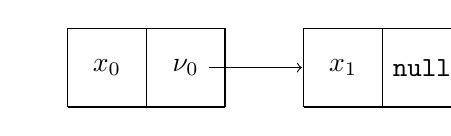
\begin{tikzpicture}
  \draw (0,0) grid (2,1);
  \draw (3,0) grid (5,1);
  \node at (0.5,0.5) (val0) {$x_0$};
  \node at (1.5,0.5) (ref0) {$\nu_0$};
  \node at (3.1,0.5) (to) {};
  \node at (3.5,0.5) (val1) {$x_1$};
  \node at (4.5,0.5) (ref1) {{\tt null}};
  \draw [->] (ref0.east) -- (to.west);
\end{tikzpicture}
\end{center}
\caption{A singly-linked list representation of $(x_0,x_1)$.}
\label{f:singlylinked}
\end{figure}

A simple Java implementation of a singly-linked list is given in
Sect.~\ref{s:hash:singlylinked}.

\subsection{Doubly-linked lists}
Doubly-linked lists\index{list!doubly-linked} are similar, but each
entry is a triplet $(\pi_i,x'_i,\nu_i)$, where $x'_i,\nu_i$ are as in
the singly-linked case, and $\pi_i$ is a reference to the
previous\index{list!previous} list entry $x_{i-1}$. The reference
$\pi_0$ of the first list element holds the {\tt null} address  (see
Fig.~\ref{f:doublylinked}).
\begin{figure}[!ht]
\begin{center}
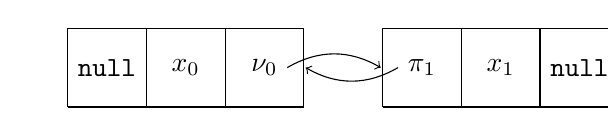
\begin{tikzpicture}
  \draw (0,0) grid (3,1);
  \draw (4,0) grid (7,1);
  \node at (0.5,0.5) (prev0) {{\tt null}};
  \node at (1.5,0.5) (val0)  {$x_0$};
  \node at (2.5,0.5) (next0) {$\nu_0$};
  \node at (2.9,0.5) (to0) {};
  \node at (4.1,0.5) (to1) {};
  \node at (4.5,0.5) (prev1) {$\pi_1$};
  \node at (5.5,0.5) (val1) {$x_1$};
  \node at (6.5,0.5) (ref1) {{\tt null}};
  \draw [->] (next0.east) to[bend left] (to1.west);
  \draw [->] (prev1.west) to[bend left] (to0.east);
\end{tikzpicture}
\end{center}
\caption{A doubly-linked list representation of $(x_0,x_1)$.}
\label{f:doublylinked}
\end{figure}

\subsubsection{The placeholder node}
In doubly-linked lists implementations, it is common to replace the
two {\tt null} references at the beginning and end of the list with a
{\it placeholder}\index{placeholder}\index{list!placeholder} entry
denoted by $\bot$. The placeholder holds a selected value whose
meaning is understood by the program to mean ``first'' or ``last''
according as to whether it precedes the first entry or succeeds the
last entry, as shown in Fig.~\ref{f:dllist}.
\begin{figure}[!ht]
\begin{center}
\psfrag{T}{$\bot$}
\psfrag{x1}{$x_0$}
\psfrag{x2}{$x_1$}
\psfrag{x3}{$x_2$}
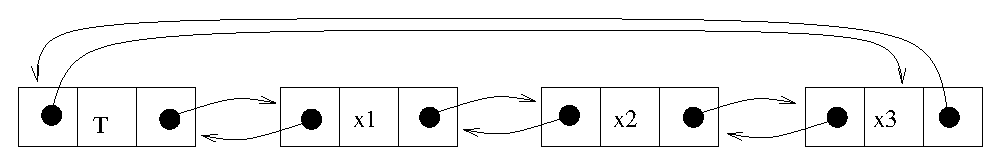
\includegraphics[width=10cm]{dllist}
\end{center}
\caption{The placeholder node (leftmost) in a doubly-linked list
  representation of $(x_0,x_1,x_2)$.}
\label{f:dllist}
\end{figure}

\subsection{Lists modelled as graphs}
It should appear clear from the pictures that we can draw a parallel
between lists and graphs:\index{graph} list entries are
nodes\index{node} or vertices,\index{vertex} and the reference
relation (the arrow) is represented by an arc\index{arc} or
edge.\index{edge} More precisely, a singly-linked list can be
represented by a simple directed path\index{path!directed}
(Fig.~\ref{f:listgraph}, left), and a doubly-linked list can be
represented by a simple (undirected) path;\index{path!simple} if a
placeholder\index{placeholder} is used, the doubly-linked list is
represented by a simple cycle\index{cycle!simple}
(Fig.~\ref{f:listgraph}, right).
\begin{figure}[!ht]
\begin{center}
\begin{minipage}{5cm}
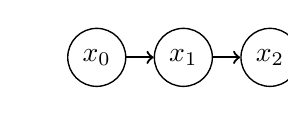
\begin{tikzpicture}
\GraphInit[vstyle=Normal]
\SetGraphUnit{1.1}
\SetVertexMath
\Vertex{x_0}
\EA(x_0){x_1}
\EA(x_1){x_2}
\Edges[style={->}](x_0,x_1,x_2)
\end{tikzpicture}
\end{minipage}
\hspace*{1cm}
\begin{minipage}{5cm}
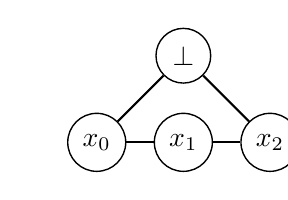
\begin{tikzpicture}[scale=1]
\GraphInit[vstyle=Normal]
\SetGraphUnit{1.1}
\SetVertexMath
\Vertex[L=\bot]{T}
\SOWE(T){x_0}
\EA(x_0){x_1}
\EA(x_1){x_2}
\Edges(T,x_0,x_1,x_2,T)
\end{tikzpicture} 
\end{minipage}
\end{center}
\caption{Singly-linked and doubly-linked lists for $(x_0,x_1,x_2)$ in
  the graph representation.}
\label{f:listgraph}
\end{figure}

\subsection{List operations}
\index{list!operation}
In this section we describe the basic operations of doubly-linked
lists with a placeholder.

\subsubsection{Insertion}
\index{list!insertion}
Consider a doubly-linked list storing $(x_0,x_1,x_2)$ and represented
as the simple cycle\index{cycle!simple} shown below.
\begin{center}
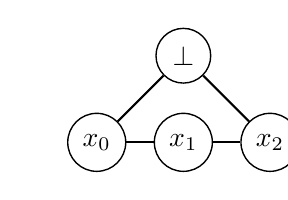
\begin{tikzpicture}[scale=1]
\GraphInit[vstyle=Normal]
\SetGraphUnit{1.1}
\SetVertexMath
\Vertex[L=\bot]{T}
\SOWE(T){x_0}
\EA(x_0){x_1}
\EA(x_1){x_2}
\Edges(T,x_0,x_1,x_2,T)
\end{tikzpicture} 
\end{center}
In order to insert an element $y$ at position 1, we proceed as
follows: we remove the edge\index{edge!removal} $\{x_0,x_1\}$, we add
a new vertex\index{vertex!addition} $y$, then add
edges\index{edge!addition} $\{x_0,y\}$ and $\{y,x_1\}$.
\begin{center}
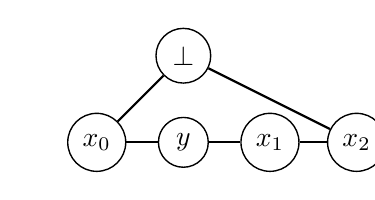
\begin{tikzpicture}[scale=1]
\GraphInit[vstyle=Normal]
\SetGraphUnit{1.1}
\SetVertexMath
\Vertex[L=\bot]{T}
\SOWE(T){x_0}
\EA(x_0){y}
\EA(y){x_1}
\EA(x_1){x_2}
\Edges(T,x_0,y,x_1,x_2,T)
\end{tikzpicture} 
\end{center}

This can be generalized. Given a doubly-linked list
$x=(x_0,\ldots,x_{n-1})$ and new element $y$ to be inserted at
position $i\in\{0,\ldots,n-1\}$, we proceed as follows:
\begin{enumerate}
\item remove edge $\{x_{i-1},x_i\}$
\item add vertex $y$
\item add edges $\{x_{i-1},y\}$ and $\{y,x_i\}$.
\end{enumerate}
This involves 4 elementary operations on the
graph,\index{graph!operation} yielding an $O(1)$ method in the worst
case.

\subsubsection{Removal}
Given a doubly-linked list $x=(x_0,\ldots,x_{n-1})$ and an index
$i\in\{0,\ldots,n-1\}$, removing\index{list!removal} the element $x_i$
is as follows:
\begin{enumerate}
\item remove vertex $x_i$ (recall from
  Sect.~\ref{s:graph:operation:addrem} that removing a
  vertex\index{vertex!removal} also removes its associated
  cutset)\index{cutset}
\item add the edge $\{x_{i-1},x_{i+1}\}$.
\end{enumerate}

\begin{ex}
Show that removal is $O(1)$ in the worst case. What is the average
case complexity?
\end{ex}

\subsubsection{Find}
\label{s:list:find}
Given a doubly-linked list $x=(x_0,\ldots,x_{n-1})$ with placeholder
$\bot$ stored both before $x_0$ and after $x_{n-1}$, an index
$i\in\{0,\ldots,n-1\}$, and a value $b$ of the same data
type\index{data!type} as the list, the find operation is as follows:
if $b\in x$ then return $x_j$ such that $x_j=b$, else return
$\bot$. This can be implemented by travelling along the
cycle,\index{cycle} starting at vertex $x_i$, traversing vertices
$x_{i+1},x_{i+2},\ldots$ until either $x_j=b$ for some $j$, or
$x_j=\bot$. We then return $x_j$.

\begin{ex}
Show that find is an $O(n)$ method in the worst case. Compute the
average case complexity\index{complexity!average case} assuming $x$ is
an array holding binary values.
\end{ex}

\subsubsection{Access}
Accessing\index{list!access}\index{list!read}\index{list!write} list
element $i$ means reading it or changing its value. Since list entries
are non-contiguous, index arithmetic\index{index!arithmetic} is
meaningless. Accordingly, we must start at the vertex labelled $x_0$
and travel along the cycle in the direction of increasing indices,
counting the vertices and stopping at the $i$-th one, then perform the
read or write operation. The worst-case is whenever $i=n-1$, which
yields $O(n)$ methods for both reading and writing.

\begin{ex}
Show that a simple implementation of a method for computing the list
size has $O(n)$ worst case complexity; point out how to implement an
$O(1)$ size operation.
\end{ex}

\subsubsection{Other operations}
The following table details list operations with the corresponding
worst-case complexity.
\begin{center}
\begin{tabular}{|l|l|} \hline
{\it Operation} & {\it Complexity} \\ \hline
Access $i$-th entry & $O(n)$ \\
Find next node having given value & $O(n)$ \\
Size & $O(n)$ or $O(1)$ \\  
Is the list empty? & $O(1)$ \\
Access first/last node & $O(1)$ \\
Remove element at given position & $O(1)$ \\
Insert element at given position & $O(1)$ \\
Move subsequence to given position & $O(1)$ \\ 
Pop from front/back & $O(1)$ \\
Push to front/back & $O(1)$ \\
Concatenate & $O(1)$ \\
\hline
\end{tabular}
\end{center}

Three operations, {\it push},\index{push}\index{see {stack, push}}
{\it pop}\index{pop}\index{see {stack, pop}} and {\it
  concatenate},\index{concatenate} have never been introduced
before. Pushing and popping are terms connected with
stacks,\index{stack} which we shall discuss in
Sect.~\ref{s:linear:stack}. In the context of lists, pushing an
element at the front or back\index{list!push} of a list means to add
an element at the first or last position; popping\index{list!pop}
means removing. Concatenating\index{list!concatenate} a list
$x=(x_0,\ldots,x_{n-1})$ and a list $y=(y_0,\ldots,y_{m-1})$ yields
the list $(x_0,\ldots,x_{n-1},y_0,\ldots,y_{m-1})$.

\subsection{Java implementation}
We propose a very simple doubly-linked list
implementation,\index{list!Java}\index{list!implementation} stored in
the text file {\tt DLList.java},\index{DLList@{\tt DLList}} structured in two
classes: {\tt Node} and {\tt DLList}. The latter, since it has the
same name as the file that stores it, also has the point of
entry\index{point of entry} {\tt main}.\index{main@{\tt main}} We remark
that neither class is declared {\tt static};\index{static@{\tt static}}
consequently, objects of these classes are not automatically allocated
in memory:\index{memory!allocation!automatic} they must be allocated
manually\index{memory!allocation!manual} using the {\tt
  new}\index{new@{\tt new}} operator.

In our implementation, every {\tt DLList} element is a {\tt Node}
object. Each {\tt Node} has references\index{reference} to
previous\index{list!previous} and next\index{list!next} nodes in the
list, and has methods for inserting other nodes after itself, removing
itself from the list, as well as printing its own data contents. The
{\tt DLList} stores a reference to the $\bot$\index{$\bot$} node, and
implements all other list methods. We emphasize that leaner
implementations of a doubly-linked list are possible: specifically, it
is possible (and also desirable\footnote{If you, as a student, are
  required in an exam to propose a linked list implementation, it is
  safe to assume that you should target a one-class implementation.})
to implement a list using only one class, such as the singly-linked
list\index{list!singly-linked} implementation given in
Sect.~\ref{s:hash:singlylinked}. We hope our implementation will also
give readers an idea of the interplay between two different classes in
the same program.

The {\tt main} method is not strictly necessary: data structure
implementations usually provide {\it libraries},\index{library}
employed by users within other programs.

\subsubsection{The {{\tt Node}} class}
As usual, we begin the file {\tt DLList.java} by writing appropriate
header comments\index{comment} and declaring useful imports.
\index{import}
{\small
\begin{verbatim}
class Node {
    public Node prev;
    public Node next;
    public int datum;

    public void remove() {
        this.prev.next = this.next;
        this.next.prev = this.prev;
    }

    public void insert(Node M) {
        this.prev = M;
        this.next = M.next;
        M.next = this;
        this.next.prev = this;
    }

    public void print() {
        System.out.print(this.datum + " ");
    }
}
\end{verbatim}
} 

As previously mentioned, a {\tt Node} stores a
reference\index{reference} to previous and next elements in the list,
as well as a piece of data (the {\tt datum}, which in this case has
{\tt int} type). The {\tt this}\index{this@{\tt this}} keyword may help
disambiguate equally named attributes of different
objects\index{object} of the same class. The piece of code that
executes {\tt this} belongs to a specific object in
memory:\index{memory!object} {\tt this} contains the address where
this object is stored.

Removal of a node works by setting its previous node's {\tt next}
attribute to its next node's {\tt previous} attribute, and vice-versa,
as shown in Fig.~\ref{f:list:remove:java}.
\begin{figure}[!ht]
\begin{center}
\begin{minipage}{5cm}
\begin{center}
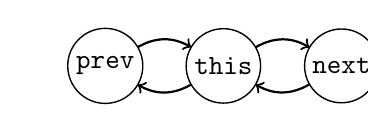
\begin{tikzpicture}
\SetVertexNormal
\SetGraphUnit{1.5}
\Vertex[L={\tt prev}]{prev}
\EA[L={\tt this}](prev){this}
\EA[L={\tt next}](this){next}
\tikzset{EdgeStyle/.append style={->,bend left}}
\Edge(prev)(this)
\Edge(this)(next)
\Edge(next)(this)
\Edge(this)(prev)
\end{tikzpicture}
\end{center}
\end{minipage}
$\overrightarrow{\mbox{\scriptsize remove {\tt this}}}$
\begin{minipage}{5cm}
\begin{center}
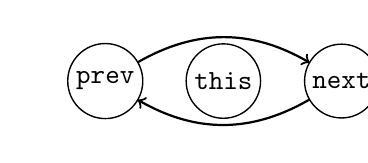
\begin{tikzpicture}
\SetVertexNormal
\SetGraphUnit{1.5}
\Vertex[L={\tt prev}]{prev}
\EA[L={\tt this}](prev){this}
\EA[L={\tt next}](this){next}
\tikzset{EdgeStyle/.append style={->,bend left}}
\Edge(prev)(next)
\Edge(next)(prev)
\end{tikzpicture}
\end{center}
\end{minipage}
\end{center}
\caption{Implementing a {\tt Node}'s removal.}
\label{f:list:remove:java}
\end{figure}

Insertion is similar to removal, but the point of view of the code
changes: {\tt this} becomes the previous node of the new node being
inserted (called {\tt M} in the code above).

\subsubsection{The {\tt DLList} class}
As for the {\tt functionPlot} example, we give the {\tt
  DLList}\index{DLList@{\tt DLList}} class structure first: this code will
not be functional until all the class method
implementations\index{class!implementation} have been filled in.
{\small
\begin{verbatim}
class DLList {
    public Node bot; // the beginning/end-of-list placeholder
    public DLList(); // class constructor
    public Node first(); // return the first element
    public Node last();  // return the last element
    public void pushBack(int t); // insert a new element t after the last one
    public int popBack(); // return last element's datum and remove from list
    public int size();    // return the list size
    public void print();  // print the whole list
    public Node find(int b); // return the first node containing datum b
    public Node findNext(Node x, int b); // start looking from Node x
    public static void main(String[] args); // the point-of-entry
}
\end{verbatim}
} 
The only attribute of the {\tt DLList} class is the {\tt
  bot}\index{bot@{\tt bot}} node, which implements the
$\bot$\index{$\bot$} placeholder.\index{placeholder} The other class
members are all methods. All members are {\tt public}.\index{public@{\tt
    public}} (this decision is somewhat arbitrary, and dictated by
simplicity: usually, attributes are private and methods are public).

The first method, which has the same name as the class and has no
return type\index{return!type}, is known as the {\it
  constructor}\index{constructor} of the
class.\index{class!constructor} It is called whenever a program issues
the instruction
\begin{verbatim}
  DLList myList = new DLList();
\end{verbatim}
in order to manually allocate some memory to the
reference\index{reference} {\tt myList}. Constructors are mostly used
to allocate memory\index{memory!allocation} and/or initialize some
variables\index{variable!value!default} with default values
{\small
\begin{verbatim}
    public DLList() {
        this.bot = new Node();
        this.bot.prev = bot;
        this.bot.next = bot;
        this.bot.datum = 0;
    }
\end{verbatim}
} The {\tt first}\index{list!first} and {\tt last}\index{list!last}
methods return the first and last elements of the list respectively.
{\small
\begin{verbatim}
    public Node first() {
        return bot.next;
    }
    public Node last() {
        return bot.prev;
    }
\end{verbatim}
} The {\tt pushBack}\index{list!push} method inserts a new list
element after the last, and {\tt popBack}\index{list!pop} returns the
last element, then removes it.  {\small
\begin{verbatim}
    public void pushBack(int t) {
        Node N = new Node();
        N.datum = t;
        N.insert(this.last());
    }
    public int popBack() {
        int t = this.last().datum;
        this.last().remove();
        return t;
    }
\end{verbatim}
} Our implementation of the {\tt size}\index{list!size} method is not
efficient, as it takes $O(n)$ in the worst case.  {\small
\begin{verbatim}
    public int size() {
        int t = 0;
        Node x = first();
        while(x != bot) {
            t++;
            x = x.next;
        }
        return t;
    }
\end{verbatim}
} The {\tt print}\index{list!print} method prints the whole list
{\small
\begin{verbatim}
    public void print() {
        Node x = first();
        while(x != bot) {
            x.print();
            x = x.next;
        }
        System.out.println();
    }
\end{verbatim}
}The {\tt find}\index{list!find} method looks for a node containing
the given argument in its {\tt datum} attribute. The {\tt
  findNext}\index{list!find next} method does the same but starts
looking from a given node {\tt x}.  {\small
\begin{verbatim}
    public Node find(int b) {
        return findNext(bot.next, b);
    }
    public Node findNext(Node x, int b) {
        bot.datum = b;
        while(x.datum != b) {
            x = x.next;
        }
        return x;
    }
\end{verbatim}
}

\subsubsection{The {\tt main} function}
We give below a possible {\tt main} function, just for validation
purposes.
{\small
\begin{verbatim}
    public static void main(String[] args)  {
        // in order to call those attributes/methods which are NOT
        // static, you need to first instantiate a dynamic object
        // of the class
        DLList dl = new DLList();

        System.out.println("size=" + dl.size());
        dl.pushBack(4);
        dl.pushBack(3);
        dl.pushBack(7);
        System.out.print("list is now "); 
        dl.print();
        System.out.println("popping last element: " + dl.popBack());
        System.out.print("list is now "); 
        dl.print();
        dl.pushBack(5);
        dl.pushBack(9);
        dl.pushBack(4);
        System.out.print("list is now "); 
        dl.print();
        System.out.println("finding node containing 9");
        Node N = dl.find(9);
        if (N != dl.bot) {
            System.out.println("deleting node containing 9");
            N.remove();
        }
        System.out.print("list is now "); 
        dl.print();
    }
\end{verbatim}
}

\section{Queues}
\label{s:linear:queue}
A {\it queue}\index{queue} is a linear data structure with four
important operations:
\begin{itemize}
\item insert\index{queue!insert} a new element at the end of the
  queue\index{queue!end}
\item retrieve\index{queue!retrieve} and delete\index{queue!delete}
  the element at the beginning of the queue\index{queue!beginning}
\item test whether the queue is empty or not\index{queue!empty}
\item find the size of the queue.\index{queue!size}
\end{itemize} 
These operations need to be performed fast: ideally, they should be
worst-case $O(1)$. Although queues can be simulated using arrays or
lists, we are going to describe a queue implementation using {\it
  circular arrays}.\index{array!circular}\index{circular array} In
queues, the first element to go in is also the first to come out. This
is known as ``first in, first out'' (FIFO).\index{FIFO}

The need for a specific implementation for queues arises because
queues grow at the end and shrink at the beginning. Imagine storing a
queue in an array: after any given number of insert operations
followed by a corresponding retrieve/delete, the queue has the same
length but has ``moved'' somewhere else in memory. Eventually the
array will exhaust its allocated space, even though the number of
stored elements may be constant (see Fig.~\ref{f:qgrow}).
\begin{figure}[!ht]
\begin{center}
  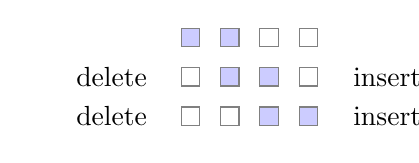
\begin{tikzpicture}
   [scale=0.5,
   queue/.style={rectangle,draw=black!50,fill=blue!20},
     arr/.style={rectangle,draw=black!50}]
  \node at (0,2) [queue] (q11) {\ };
  \node at (1,2) [queue] (q12) {\ };
  \node at (2,2) [arr] (a13) {\ };
  \node at (3,2) [arr] (a14) {\ };
  \node at (0,1) [arr] (a21) {\ };
  \node at (1,1) [queue] (q22) {\ };
  \node at (2,1) [queue] (q23) {\ };
  \node at (3,1) [arr] (a24) {\ };
  \node at (0,0) [arr] (a31) {\ };
  \node at (1,0) [arr] (a32) {\ };
  \node at (2,0) [queue] (q33) {\ };
  \node at (3,0) [queue] (q34) {\ };
  \node at (-2,1) (del1) {delete};
  \node at (5,1) (ins1) {insert};
  \node at (-2,0) (del2) {delete};
  \node at (5,0) (ins2) {insert};
\end{tikzpicture}
\end{center}
\caption{A queue worms its way along the array, exhausting and wasting
  space.}
\label{f:qgrow}
\end{figure}

\subsection{Circular arrays}
\label{s:linear:circarray}
The appropriate graph model for a circular array of size $n$ is a
cycle\index{cycle} with $n+1$ vertices (see Fig.~\ref{f:qcycle}).
\begin{figure}[!ht]
\begin{center}
\begin{tikzpicture}[scale=1.5]
\GraphInit[vstyle=Normal]
\SetGraphUnit{1.1}
%\SetVertexMath
\SetVertexNoLabel
\Vertices{circle}{q_2,q_1,q_0,q_9,q_8,q_7,q_6,q_5,q_4,q_3}
\Edges(q_0,q_9,q_8,q_7,q_6,q_5,q_4,q_3,q_2,q_1,q_0)
\end{tikzpicture}
\end{center}
\caption{The graph representation of a circular array: a cycle.}
\label{f:qcycle}
\end{figure}

Let $C=(V,E)$ be a cycle: we define $V=\{q_0,\ldots,q_n\}$ and
$E=\{\{q_i,q_{i+1}\}\;|\;i\in\{0,\ldots,n-1\}\}$. At each
vertex\index{vertex} of $V$ we store the address\index{object!address}
of an object of the same class, or a {\tt null}\index{null@{\tt null}}
address denoted by $\bot$. We want to store a queue\index{queue}
$d=(d_0,\ldots,d_t)$ in $C$, in such a way that whenever the queue
``advances'' in memory, by means of repeated
insertions\index{queue!insertion} at one end and
removals\index{queue!removal} at the other end (but keeping its
size\index{queue!size} constant), the storage will ``cycle'' through
$C$, re-occupying the same memory cells\index{memory!cell} whenever
these are empty (see Fig.~\ref{f:q1}). Obviously, we have to make the
assumption that the size $t$ of the queue will never exceed the size
$n$ of the circular array.
\begin{figure}[!ht]
{\small
\begin{center}
\begin{minipage}{4cm}
\begin{center}
\begin{tikzpicture}
  [scale=0.9,memory/.style={rectangle,draw=black!50,fill=blue!20}]  
  \node (d0) at (90:1.5) [memory] {\ } ;
  \node (q0) at (90:2.0) {$q_0$} ;
  \node (d1) at (54:1.5) [memory] {\ } ;
  \node (q1) at (54:2.0) {$q_1$} ;
  \node (d2) at (18:1.5) [memory] {$d_0$} ;
  \node (q2) at (18:2.0) {$q_2$} ;
  \node (d3) at (-18:1.5) [memory] {$d_1$} ;
  \node (q3) at (-18:2.0) {$q_3$} ;
  \node (d4) at (-54:1.5) [memory] {$d_2$} ;
  \node (q4) at (-54:2.0) {$q_4$} ;
  \node (d5) at (-90:1.5) [memory] {$d_3$} ;
  \node (q5) at (-90:2.0) {$q_5$} ;
  \node (d6) at (-126:1.5) [memory] {$\bot$} ;
  \node (q6) at (-126:2.0) {$q_6$} ;
  \node (d7) at (-162:1.5) [memory] {\ } ;
  \node (q7) at (-162:2.0) {$q_7$} ;
  \node (d8) at (162:1.5) [memory] {\ } ;
  \node (q8) at (162:2.0) {$q_8$} ;
  \node (d9) at (126:1.5) [memory] {\ } ;
  \node (q9) at (126:2.0) {$q_9$} ;
\end{tikzpicture}
\end{center}
\end{minipage}
$\overrightarrow{\mbox{insert }d_4}$
\begin{minipage}{4cm}
\begin{center}
\begin{tikzpicture}
  [scale=0.9,memory/.style={rectangle,draw=black!50,fill=blue!20}]  
  \node (d0) at (90:1.5) [memory] {\ } ;
  \node (q0) at (90:2.0) {$q_0$} ;
  \node (d1) at (54:1.5) [memory] {\ } ;
  \node (q1) at (54:2.0) {$q_1$} ;
  \node (d2) at (18:1.5) [memory] {$d_0$} ;
  \node (q2) at (18:2.0) {$q_2$} ;
  \node (d3) at (-18:1.5) [memory] {$d_1$} ;
  \node (q3) at (-18:2.0) {$q_3$} ;
  \node (d4) at (-54:1.5) [memory] {$d_2$} ;
  \node (q4) at (-54:2.0) {$q_4$} ;
  \node (d5) at (-90:1.5) [memory] {$d_3$} ;
  \node (q5) at (-90:2.0) {$q_5$} ;
  \node (d6) at (-126:1.5) [memory] {$d_4$} ;
  \node (q6) at (-126:2.0) {$q_6$} ;
  \node (d7) at (-162:1.5) [memory] {$\bot$} ;
  \node (q7) at (-162:2.0) {$q_7$} ;
  \node (d8) at (162:1.5) [memory] {\ } ;
  \node (q8) at (162:2.0) {$q_8$} ;
  \node (d9) at (126:1.5) [memory] {\ } ;
  \node (q9) at (126:2.0) {$q_9$} ;
\end{tikzpicture}
\end{center}
\end{minipage}
$\overrightarrow{\mbox{remove }d_0}$
\begin{minipage}{4cm}
\begin{center}
\begin{tikzpicture}
  [scale=0.9,memory/.style={rectangle,draw=black!50,fill=blue!20}]  
  \node (d0) at (90:1.5) [memory] {\ } ;
  \node (q0) at (90:2.0) {$q_0$} ;
  \node (d1) at (54:1.5) [memory] {\ } ;
  \node (q1) at (54:2.0) {$q_1$} ;
  \node (d2) at (18:1.5) [memory] {\ } ;
  \node (q2) at (18:2.0) {$q_2$} ;
  \node (d3) at (-18:1.5) [memory] {$d_1$} ;
  \node (q3) at (-18:2.0) {$q_3$} ;
  \node (d4) at (-54:1.5) [memory] {$d_2$} ;
  \node (q4) at (-54:2.0) {$q_4$} ;
  \node (d5) at (-90:1.5) [memory] {$d_3$} ;
  \node (q5) at (-90:2.0) {$q_5$} ;
  \node (d6) at (-126:1.5) [memory] {$d_4$} ;
  \node (q6) at (-126:2.0) {$q_6$} ;
  \node (d7) at (-162:1.5) [memory] {$\bot$} ;
  \node (q7) at (-162:2.0) {$q_7$} ;
  \node (d8) at (162:1.5) [memory] {\ } ;
  \node (q8) at (162:2.0) {$q_8$} ;
  \node (d9) at (126:1.5) [memory] {\ } ;
  \node (q9) at (126:2.0) {$q_9$} ;
\end{tikzpicture}
\end{center}
\end{minipage}
\end{center}
}
\caption{The queue ``advances'' in the memory cells of the circular 
array.}
\label{f:q1}
\end{figure}
If vertex $q_k$ contains the last queue element $d_t$ at any time,
then we store an end-of-queue placeholder\index{queue!placeholder}
$\bot$ at vertex $q_{k+1}$. In order for vertex indices never to
exceed $n$, we employ arithmetic modulo $n$ on indices (so that, e.g.,
$q_{k+1}$ is in fact $q_{k+1\pmod n}$).

\subsubsection{Java implementation}
The implementation of a circular
array\index{array!circular!implementation} is very simple; it is based
on a linear array of fixed length. All index arithmetic is carried
out modulo that length. 
{\small
\begin{verbatim}
public class circularArray {
    // attributes (private)
    int[] q;// the array
    int n;  // array size    
    int h;  // index of head element (first data element stored at q[h])
    int t;  // index of tail element (last data element stored at q[t-1])

    // methods (public)
    public circularArray(int qlen) {  // class constructor
        n = qlen;
        q = new int[n];
        h = 0;
        t = 0;
    }
    public boolean isEmpty() {  // test whether array is empty
        if (h == t) {
            return true;
        } else {
            return false;
        }
    }
    public int first() {  // return first element
        assert(!isEmpty()) : "error: queue is empty, cannot read first element";
        return q[h];
    }
    public int popFront() { // read and remove the first element
        int p = this.first();
        h = (h+1) % n;
        return p;
    }
    public int size() { // return the size 
        int theSize = (t - h + n) % n;
        return theSize;
    }
    public void pushBack(int d) { // insert new element at array end
        assert(this.size() < n) : 
        "error: queue is full: cannot push elements on its back";
        q[t] = d;
        t = (t+1) % n;  
    }
}
\end{verbatim}
} Notice that, even though any array element can be
accessed\index{array!access} in $O(1)$, the {\tt
  circularArray}\index{circularArray@{\tt circularArray}} class offers a limited
interface,\index{interface} functional to a queue:\index{queue} it is
only possible to push new elements on the back of the array and pop
elements from the front. 

Notice also that the class constructor takes an argument as input,
i.e.~the array length. Constructors can take arguments as any other
function, but their return type is not declared, since it is defined
to be the same class as they belong to.

The {\tt assert}\index{assert@{\tt assert}} is used for error
detection:\index{error!detection} if the test passed to {\tt assert}
as an argument is false, execution stops with the given error message.

\begin{ex}
Show that every method of the {\tt circularArray} class is $O(1)$.
\end{ex}

\subsection{What are queues used for?}
Queues are handy when simulating the behaviour of queues in the
physical world, be they human, car, packet or other type of
queues.\index{queue!applications} Secondly, they are essential in the
implementation of a well-known algorithm for graph
exploration,\index{graph!exploration} namely breadth-first search
(BFS).\index{breadth-first search}\index{BFS} We shall discuss BFS in
Sect.~\ref{s:graphalg:bfs}. Lastly, a queue variant called {\it
  priority queue}\index{priority queue}\index{queue!priority} (see
Sect.~\ref{s:search:heap:priorityq}) is essential to the
implementation of most algorithms for computing shortest paths in
graphs (see Chapter \ref{c:path}).

\section{Stacks}
\label{s:linear:stack}
A stack\index{stack} is similar to a queue, but instead of pushing at
the back and popping from the front, we push\index{stack!push} and
pop\index{stack!pop} from the back. A stack data structure is
appropriate in situations where the last element to be stored is the
first to be retrieved. This is known as ``last in, first out''
(LIFO).\index{LIFO}

\subsection{Using stacks for validating mathematical syntax}
At a glance, are you able to state whether the following mathematical
expression has a balanced number of brackets?
\begin{equation*}
  \left((((x+y)z-2\sin(x))+\frac{1}{2}\left(\sum_{i\le
    3}p_i^2\right))/\log((p_1(p_2-p_3^{(\cos(\tan(x)))})))\right)
\end{equation*}
One way to go about this task is to keep a counter, initially set at
zero: scanning the expression, increase the counter by one unit every
time you read an open bracket, and decrease it by one unit every time
you read a closed bracket. If the counter is always $\ge 0$ and gets
to zero by the time the scanning is over, then the brackets are
balanced. 

What if you had square brackets as well, however? A situation like
$([1+2)]$ would result in a correct balancing, but would miss the
incorrect embedding. To overcome this problem, we can use a stack:
every time an open bracket is read, push the closing corresponding
bracket on the stack. Every time a closing bracket is read, pop the
last element off the stack, and verify it is the same.  If we get to
the end of the stack at the same time the scanning ends, then the
brackets are well-balanced, otherwise the expression is wrong.

\begin{ex}
Prove the last assertion formally.
\end{ex}

\subsubsection{Java implementation}
We implement the above idea, and the associated
stack,\index{stack!implementation} in a class called {\tt
  bracketStack}. The implementation of the {\tt main} function is
given later.  {\small
\begin{verbatim}
class bracketStack {
    // attributes (private)
    int [] theStack; // the stack is implemented as an array
    int pos;         // the current stack size is stored in pos

    // methods (public)
    public bracketStack(int maxSize) { // class constructor
        theStack = new int[maxSize];
        pos = 0;
    }
    public Boolean isEmpty() { // is the stack empty?
        Boolean t = Boolean.TRUE;
        if (pos > 0) {
            t = Boolean.FALSE;
        }
        return t;
    }
    public void push(int element) { // push an element on the stack
        assert(pos < theStack.length) : "no more memory for growing stack";
        theStack[pos] = element;
        pos++;
    }    
    public int pop() {  // pop an element from the stack
        assert(!isEmpty());
        pos--;
        return theStack[pos];
    }

    // the main method
    public static void main(String[] args);
}
\end{verbatim}
}

\begin{ex}
Show that every method in this stack implementation is $O(1)$
\end{ex}

\subsubsection{The {\tt main} method for {\tt bracketStack}}
Find below the implementation of bracket-checking algorithm discussed
above. 

Notice that this code reads the mathematical expression from the
command line: it is an example of how to use the {\tt String[] args}
array. {\tt String} is a standard library\index{library!standard}
class for storing strings. When a shell command such as:
\begin{verbatim}
   java bracketStack "((([])))"
\end{verbatim}
is given, the Java compiler makes all arguments after the name of the
program (in this case, {\tt bracketStack}) available to the program
itself within the array of strings {\tt args}. More precisely, {\tt
  args[0]} contains the first command, {\tt args[1]} contains the
second, and so on. Since {\tt args} is declared as {\tt String[]},
every element is a string; we can therefore {\tt args[0].length()} to
find the length of the string stored in {\tt args[0]}. 

{\small
\begin{verbatim}
public static void main(String[] args) {

    // read bracketed sentence from cmd line
    int argSize = args[0].length();
    String theArg = args[0];

    // initialize dynamic object of this class
    bracketStack brackStack = new bracketStack(argSize);
    
    // counter is the current character index in the input sentence
    int counter = 0;

    // character popped off the stack
    int elt;

    // error status: 
    //   0 is "valid sentence"
    //   1 is "wrong closing bracket"
    //   2 is "too many closing brackets"
    //   3 is "not enough closing brackets"
    int err = 0;

    // look at every character of the input sentence
    while(counter < argSize) {

        if (theArg.charAt(counter) == '(') {
            // whenever an open round bracket is found,
            // push the closing one on the stack
            brackStack.push(')');

        } else if (theArg.charAt(counter) == '[') {
            // whenever an open square bracket is found,
            // push the closing one on the stack
            brackStack.push(']');

        } else if (theArg.charAt(counter) == ')' ||
                   theArg.charAt(counter) == ']') {
            // if any type of closing bracket is found              
            if (brackStack.isEmpty()) {
                // ...and the stack is empty, it means there are more
                // closing brackets than open ones
                err = 2;
                break;

            } else {
                // ...pop an element off the stack
                elt = brackStack.pop();
                if (elt != theArg.charAt(counter)) {
                    // if this is different from the closing bracket,
                    // it means that either an open round bracket was
                    // closed by a square one, or vice versa
                    err = 1;
                    break;
                }
            }
        }
        // increase the character counter
        counter++;
    }
    if (err == 0 && !brackStack.isEmpty()) {
        // if no error of type 1 or 2 were reported, but the stack is not
        // empty yet, it means that there were more open than closed
        // brackets
        err = 3;
    }
    
    // report status message
    if (err == 1) {
        System.out.println("wrong closing bracket at pos " + (counter+1));
    } else if (err == 2) {
        System.out.println("too many closing brackets");
    } else if (err == 3) {
        System.out.println("not enough closing brackets");
    } else {
        System.out.println("valid sentence");
    }
}
\end{verbatim}
}

\subsubsection{Sample output}
Here's some sample output from the {\tt bracketStack} program, when
called from the command line.\index{command line}
\begin{verbatim}
$ java bracketStack "((]]"
wrong closing bracket at pos 3
$ java bracketStack "(())"
valid sentence
$ java bracketStack "(())]"
too many closing brackets
$ java bracketStack "[(())]"
valid sentence
$ java bracketStack "([1+2)]"
wrong closing bracket at pos 6
$ java bracketStack "[(1+2)]"
valid sentence
\end{verbatim}

\subsection{Calling functions}
\label{s:linear:stack:function}
The main use of stacks within an operating system\index{operating
  system} (OS)\index{OS} is to simulate the function call
mechanism.\index{function!call} In fact, classic CPUs have native
instructions for transferring control\index{control} to the code
instruction\index{instruction} stored at a given memory
address\index{memory!address} (the so-called ``GOTO"\index{GOTO}
statement, also called {\tt jmp}\index{jmp@{\tt jmp}} in assembly
language),\index{language!assembly}\index{assembly} but not
necessarily a {\tt return}\index{return@{\tt return}} statement. This,
however, is easily implemented by simply storing the calling address
before {\tt jmp}ing to the new one, and then re-{\tt jmp}ing to the
stored calling address whenever a {\tt return} is issued.

Recall that a {\tt return} statement issued from a function $h$ can
only return control to the function $g$ that directly called $h$, but
not to the function $f$ that called $g$ (see
Fig.~\ref{f:functioncall}).
\begin{figure}[!ht]
\begin{center}
\psfrag{f}{$f$}
\psfrag{g}{$g$}
\psfrag{h}{$h$}
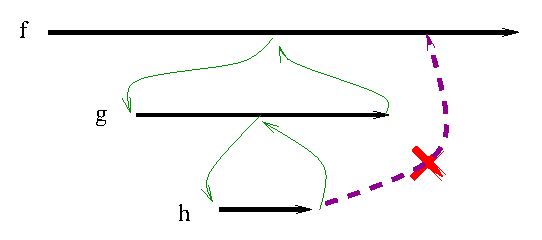
\includegraphics[width=7cm]{call_to_call}
\end{center}
\caption{The function $h$ cannot return control to $f$: it must return
  it to its direct calling function $g$.}
\label{f:functioncall}
\end{figure}
Therefore, when nested calling\index{function!call!nested} occurs, the
addresses of the calling functions can be pushed on a
stack,\index{stack} and popped at each successive {\tt return}
statement (see Fig.~\ref{f:osstack}).

\begin{figure}[!ht]
\begin{center}
\begin{tabular}{c|c}
\begin{minipage}{7.2cm}
\psfrag{f}{}
\psfrag{g}{}
\psfrag{cpuf}{$f$}
\psfrag{cmd1}{}
\psfrag{cmd2}{}
\psfrag{top1}{top}
\psfrag{top2}{}
\psfrag{top3}{}
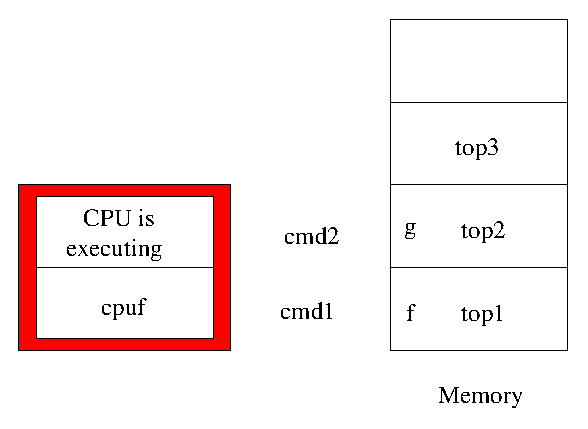
\includegraphics[width=7cm]{function_stack}
\end{minipage} &
\begin{minipage}{7.2cm}
\psfrag{f}{\tiny current state of $f$}
\psfrag{g}{}
\psfrag{cpuf}{$f${\tiny ::call $g$}}
\psfrag{cmd1}{push}
\psfrag{cmd2}{}
\psfrag{top1}{}
\psfrag{top2}{top}
\psfrag{top3}{}
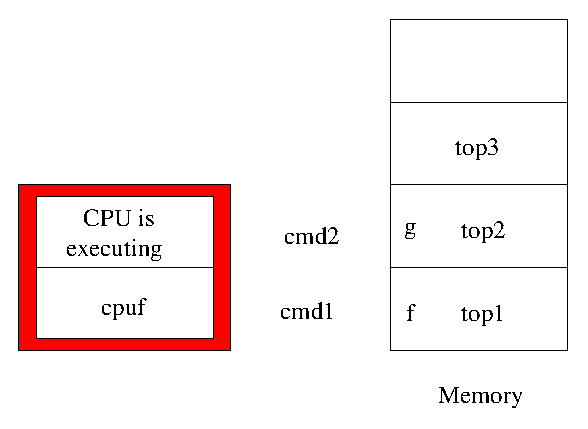
\includegraphics[width=7cm]{function_stack}
\end{minipage}\\ 
\begin{minipage}{7.2cm}
\psfrag{f}{\tiny current state of $f$}
\psfrag{g}{\tiny current state of $g$}
\psfrag{cpuf}{$g${\tiny ::call $h$}}
\psfrag{cmd1}{}
\psfrag{cmd2}{push}
\psfrag{top1}{}
\psfrag{top2}{}
\psfrag{top3}{top}
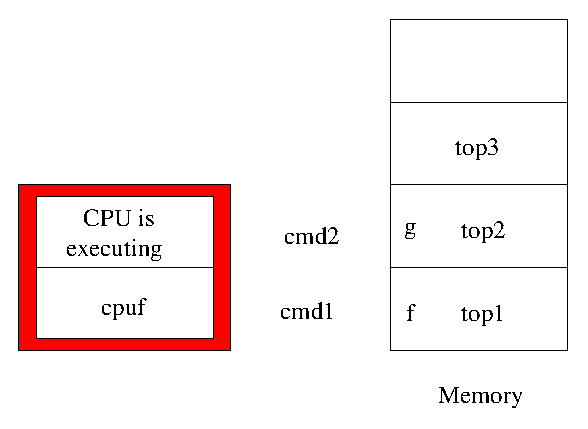
\includegraphics[width=7cm]{function_stack}
\end{minipage} &
\begin{minipage}{7.2cm}
\psfrag{f}{\tiny current state of $f$}
\psfrag{g}{\tiny current state of $g$}
\psfrag{cpuf}{$h${\tiny ::return}}
\psfrag{cmd1}{}
\psfrag{cmd2}{pop}
\psfrag{top1}{}
\psfrag{top2}{}
\psfrag{top3}{top}
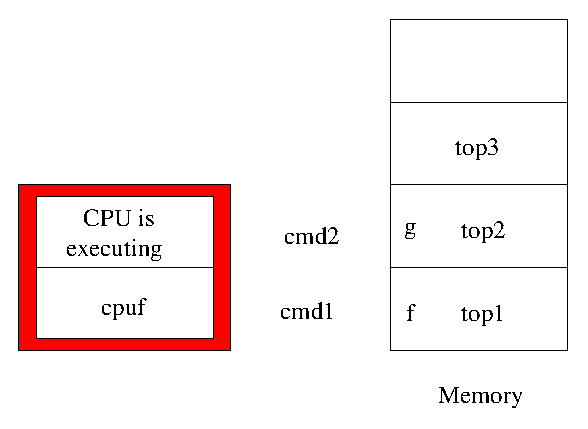
\includegraphics[width=7cm]{function_stack}
\end{minipage}
\\ 
\begin{minipage}{7.2cm}
\psfrag{f}{\tiny current state of $f$}
\psfrag{g}{}
\psfrag{cpuf}{$g${\tiny ::return}}
\psfrag{cmd1}{pop}
\psfrag{cmd2}{}
\psfrag{top1}{}
\psfrag{top2}{top}
\psfrag{top3}{}
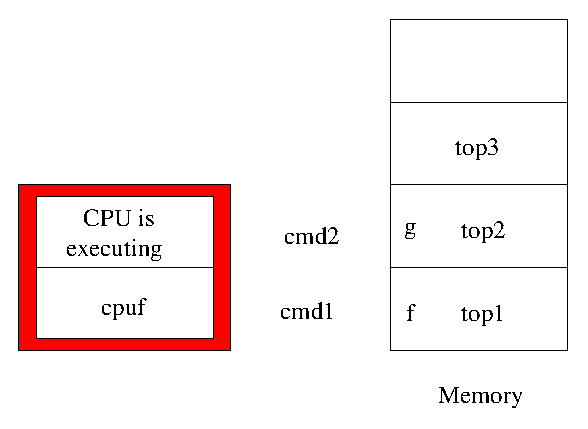
\includegraphics[width=7cm]{function_stack}
\end{minipage}
&
\begin{minipage}{7.2cm}
\psfrag{f}{}
\psfrag{g}{}
\psfrag{cpuf}{$f$}
\psfrag{cmd1}{}
\psfrag{cmd2}{}
\psfrag{top1}{top}
\psfrag{top2}{}
\psfrag{top3}{}
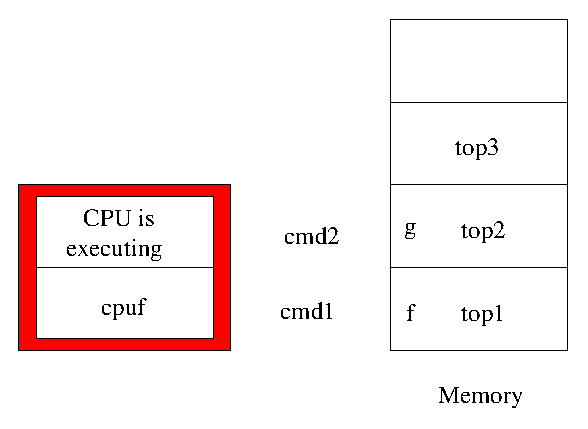
\includegraphics[width=7cm]{function_stack}
\end{minipage}
\end{tabular}
\end{center}
\caption{What happens to the OS stack as $f$ calls $g$ which calls $h$.}
\label{f:osstack}
\end{figure}

\subsubsection{Smashing the stack for fun and profit}
The first serious breaches into interconnected computer systems was
carried out by a technique called ``smashing the
stack''.\index{stack!smashing} It was based on a poor implementation
of some string input functions,\index{input} where a string was simply
a fixed-length array of characters. These input
functions\index{function!input} did not check that the length of the
user input was actually smaller than the allocated array
memory,\index{array!memory} and hence a long input would overwrite
memory past the array bounds.\index{array!bound} If the array was
allocated on the same stack used for the function calls, then a hacker
would translate some particularly nasty code into ASCII\index{ASCII}
and pass it to the string input function. On returning from the string
input function, the return address\index{address!return} was
overwritten with the nasty code, which got executed and spawned all
sorts of actions, such as opening a root shell\index{root!shell} on
the hacker's terminal (see Fig.~\ref{f:smashstack}).

\begin{figure}[!ht]
\begin{center}
\fbox{\includegraphics[width=12cm]{smashstack}}
\end{center}
\caption{The {\it Phrack} issue that made stack smashing famous.}
\label{f:smashstack}
\end{figure}

\section{Maps}
\label{s:linear:map}
Maps are representations of functions. In mathematics, a
function\index{function} $f$ from a set\index{set} $X$ to a set $Y$ as
is defined as a set $F$ of pairs\index{pair} $(x,y)$, with $x\in X$
and $y\in Y$, and such that if $y=f(x)$ and $y'=f(x)$ then
$y=y'$. This property is known as {\it
  well-definedness}\index{function!well-defined} of the
function. Correspondingly, a {\it map}\index{map} is a data
structure\index{data!structure} defined over two non-elementary data
types,\index{data!type!non-elementary} that play the role of $X$ and
$Y$, for storing well-defined\index{well-defined} pairs $(x,y)$. In
Java, a map where $X,Y$ are both integers is defined as:
\begin{verbatim}
  Map<Integer,Integer> theMap;
\end{verbatim}

\subsection{Maps as parametrized interfaces}
\label{s:linear:map:parametrized}
Two remarks are in order. First, a {\tt Map}\index{Map@{\tt Map}} is an
interface (see Sect.~\ref{s:java:interface}) rather than a class ---
Java offers different implementations of a map. 

Second, a Java {\tt Map} is {\it
  parametrized}\index{class!parametrized} over two other classes. This
is common in {\it generic containers}:\index{generic container} these
are data containers, such as arrays, lists, maps and so on, whose code
is object-independent: in other words, objects of any class can be
stored in such containers, it suffices that the ``parameter
class''\index{class!parameter} be declared in the program by using the
angle bracket notation {\tt <>}.\index{<>@{\tt <>}} A requirement for the
parameter class is that it should be a non-elementary data
type.\index{data!type!non-elementary} In our case, since {\tt int} is
an elementary data type, we use the non-elementary equivalent {\tt
  Integer}.\index{Integer@{\tt Integer}}

We remark that classes can also be parametrized (as well as
interfaces), and that a common name in the literature for
parametrizing a type\index{type!parametrized} with another type is
{\it template}.\index{template}

\subsection{Example of map usage in Java}
See the following example of the use of a Java map, implemented as a
{\tt HashMap} (see Ch.~\ref{c:hash} for details about hashing).
\begin{verbatim}
  Map<String,Integer> phonebook = new HashMap<String,Integer>();
  phonebook.put("Leo", 169334138);
  phonebook.put("Tom", 169334425);
  System.out.println("Leo's phone number is 0" + phonebook.get("Leo"));
\end{verbatim}

%%%%%%%%%%%%%%%%% CHAPTER: HASHING %%%%%%%%%%%%%%%%%%%%%%%%%%
\chapter{Hashing}
\label{c:hash}

\begin{center}
\fbox{\begin{minipage}{13cm}{\small {\sc Abstract}.  Hashing:
      efficiently finding items in a large-sized array. Motivation,
      example, Java implementations.  }
\end{minipage}}
\end{center}


A {\it hash table}\index{hash table} is a data structure for storing a
function $\tau:K\to U$, where $K$ is a set of {\it keys}\index{key}
and $U$ is a set of {\it records}\index{record}, so that $\tau(k)$ can
be retrieved efficiently from memory.

\section{Do we really need it?}
\label{s:hash:critique}
The definition of a hash table might appear puzzling at first sight:
why not store functions by means of lists or arrays? We saw in
Sect.~\ref{s:list:find} that retrieving a specific element of a
list\index{list} takes time proportional to the list length. Hence,
storing the pairs (key, record) in a list will not yield a
retrieval-efficient data structure. What about an array,\index{array}
however? After all, if {\tt a} is an array of records, and {\tt i} is
an {\tt int}, then {\tt a[i]} is retrieved in constant
time\index{constant time} by simply looking up the value stored at the
memory address\index{memory!address} indexed by the base
address\index{base address} of {\tt a} plus {\tt i} times the number
of bytes taken to store an {\tt int}. If, however, the function {\tt
  a} were to map integers from the set $K=\{1,16,1643,1094382\}$,
using an array would require allocating space for $1094382$ elements,
although we would only use four of them: definitely too wasteful.

What if our keys are names, as might happen in a telephone directory?
We could address this issue by listing all possible names in an order,
and then remember the order rank\index{order!rank} of each name. This
has drawbacks. Storing the assignment\index{assignment} (name, rank)
would take a huge amount of memory if we wanted to do this for {\it
  every possible name in existence}: and besides, we would have simply
shifted the problem to efficiently scan this assignment between names
and ranks. Suppose now we choose an alphabetical
order,\index{order!alphabetical} and only limit the assignment to a
given subset of names (for example, those names corresponding to
people we know). As we get to meet new people, we need to store their
names in the subset. Thus, we have to insert new elements in the
assignment: if this is stored as an array,\index{array} we know from
Sect.~\ref{s:array:operations} that insertion\index{array!insert}
takes time proportional to the array length, which may turn out to be
too slow if the array grows considerably.

In summary, neither lists nor arrays provide the efficient data
structure we are looking for: and this motivates the definition of a
hash table.

\subsection{The phonebook example}
\label{s:hash:phonebook}
The solution is given by a phonebook. This consists of a notebook
whose pages are indexed with letters: A, B, \dots, Z. One writes a
name and the corresponding telephone number (say ``Leo Liberti,
0169334138'') into the page indexed by the initial letter of the
surname (`L' in this case). Every page has a finite length, but we
assume the mechanism is unlikely to fail because most people have
fewer acquaintances whose names begin with a specific letter than can
be written in a page. Thus, in order to find the key ``Leo Liberti''
in the phonebook and retrieve the record ``0169334138'', it suffices
to identify the correct page, and then to scan the whole page for the
correct key. Identifying the correct page is an operation that
requires constant time, since the page position from the beginning is
proportional to the position of the corresponding letter with respect
to the first alphabet letter `A', and the size of the alphabet is a
constant. The time taken by scanning each page is at worst
proportional to the page length, which is constant over the whole
notebook --- hence this time is also constant. Overall, then, a
phonebook allows you to find a pair (key, record) in constant time,
independently of the actual number of phonebook entries, as long as
they fit in the phonebook.

Here is some good news: if you understood this phonebook example, you
understood the idea of hashing.

\subsection{Formal explanation}
Now keep the phonebook of Sect.~\ref{s:hash:phonebook} in mind and let
$K$ be a set of keys, $U$ be a set of records, and $\tau$ be a table
mapping a subset of $K$ to $U$. We denote by $\dom{\tau}$ the
domain\index{domain} of $\tau$, and assume that $\dom{\tau}$ is
``small'' with respect to $K$. Using the phonebook example metaphor:
there are many millions, perhaps billions of names in the world, but
the set of your acquaintances counts dozens, hundreds or in the most
extreme case thousands, of names.

Consider a set $I$ of indices\index{index}, which we shall assume
for simplicity to be $\{0,1,\ldots,p-1\}$, of cardinality ``more or
less'' like that of $U$. By ``more or less'' we mean that $|I|$ is
$O(|U|)$. Also consider a {\it hash function}\index{hash function}
$h:K\to I$ that maps keys to indices. Finally, consider an array
$\sigma$, indexed by $I$, whose elements are linear data structures of
some type (e.g.~arrays or lists), all having the same fixed size
$\alpha$.\index{data!structure!fixed size} For any $k\in\dom{\tau}$, we 
store
$\tau(k)$ in the hash table $\sigma$, within the fixed size linear
data structure $\sigma(h(k))$ (see Fig.~\ref{f:hash}).
\begin{figure}[!ht]
\begin{center}
\psfrag{K}{$K$}
\psfrag{U}{$U$}
\psfrag{tau}{$\tau$}
\psfrag{domtau}{$\dom\tau$}
\psfrag{sigma}{$\sigma$}
\psfrag{h}{$h$}
\psfrag{I}{$I$}
\includegraphics[width=10cm]{minimal3}
\end{center}
\caption{Hashing.}
\label{f:hash}
\end{figure}
Should two distinct keys\index{key} $k,k'$ be mapped by $h$ to the
same index\index{index} $i$, then the corresponding
records\index{record} $\tau(k),\tau(k')$ would both be stored in the
fixed size linear data structure $\sigma(i)$. This assumes that no
more than $\alpha$ keys are mapped by $h$ to the same index.

In the phonebook metaphor, $h$ maps names to their initials, we assume
that no phonebook user has more similarly-initialled acquaintances
than the $\alpha$ lines in each page of the phonebook $\tau$, and if
we have a name $k$ with initial $h(k)$, we write the corresponding
record on the page indexed by $h(k)$.

\subsection{Applications of hashing to Java}
Aside from the phonebook, hash tables are often used for storing maps
(see the {\tt HashMap} class used in Sect.~\ref{s:linear:map}). 

Hash functions (the function $h$ mapping keys to indices) also have
very useful applications of their own. In Java
programming,\index{Java!programming} for example, objects often occupy
sizable chunks of memory; if we need to know whether two separate
objects $a,b$ of the same class $C$, stored at different addresses,
contain the same data,\index{object!equal} we have to run a byte
comparison\index{comparison!byte} on the memory occupied by $a$ and
$b$. This will run in time $O(\max(|a|,|b|))$, where $|a|,|b|$ are the
memory sizes\index{memory!size} of $a,b$ respectively. The way this
can be done in $O(1)$ is by devising an injective hash
function\index{hash function!injective} $h:C\to {\tt int}$ that
computes an integer code for unique to each object in the class
$C$. This way, $a=b$ if and only if $h(a)=h(b)$ (the latter test can
be done in constant time).

Although it is very difficult to construct a hash function that is
guaranteed to be injective, it is not too hard to only require $h$ to
be injective with high probability (i.e.~minimizing the occurrences
that $a\not=b$ even though $h(a)=h(b)$). Java offers a default hash
function, called {\tt hashCode()},\index{hashCode@{\tt hashCode}} that applies
to every class:
\begin{verbatim}
  public class C { ... };
  // ...
  C a = new C();
  C b = new C();
  // ...
  if (a.hashCode() == b.hashCode()) {
    System.out.println("a = b");
  }
\end{verbatim}
Since the Java developers recognize that more efficient hash functions
can be developed by the programmers in certain instances, the {\tt
  hashCode} function can be {\it
  overloaded}\index{function!overloading} (i.e., replaced by a
user-defined function with the same name and taking the same number
and type of arguments). 

\section{The last nagging doubt}
Perhaps some readers are still doubtful of hash functions. After all,
they will argue, we need to store the map\index{map} $h:K\to I$
somewhere, and we are just shifting the problem again. We cannot use a
list\index{list} because searching is inefficient, and we cannot use
an array\index{array} because it would either take too much memory to
store, or too long to insert new pairs (key, index), just as it
happened in Sect.~\ref{s:hash:critique}

Here is where the magic lies: {\it we do not need to store $h$
  explicitly}. The hash function $h$ is computed directly by the data
representation of $k$. If $k$ is a name, for example, it is encoded as
a string of characters; each character corresponds to an integer
between 0 and 255 called its ASCII\index{ASCII} code: hence a name of
$n$ letters is simply a sequence in $\{0,\ldots,255\}^n$. Any
algorithm that takes such a sequence $k$ as input and outputs a single
integer $i\in I$ defines a hash function $h:K\to I$. In order for the
whole scheme to work, however, we need $h$ to be computed in constant
time. This is obtained by: coding efficiently and carefully, and
setting a fixed limit to the key lengths (or only considering a fixed
amount of information in each key) when computing $h$.

For example, a very simple (certainly not injective) hash function
between names and integers would associate to a character string the
sum of the ASCII character codes, modulo the largest possible
representable integer. The name ``Leo'' would be hashed to
$76+101+111=288$, because the ASCII codes of `L', `e', `o' are
$76,101,111$. Thus we could store the record for the key ``Leo'' in a
linear data structure stored at $\sigma(288)$.

\section{Java implementation}
We are going to present two different implementations of a hash
table\index{hash table} $\sigma$. The first one is simpler, and
assumes the hash function $h$ is injective.\index{hash
  function!injective} As a consequence, each linear data structure in
$\sigma(h(k))$ only ever holds one record (why?): in other words,
$\sigma$ need not be an array of linear data structures that contain
records,\index{record} but only an array that directly contains
records. The second implementation does not assume $h$ to be
injective, allows {\it collisions}\index{collision} (i.e.~more keys
mapped to the same index), and uses singly-linked
lists\index{list!singly-linked} as linear data structures to be stored
in the array $\sigma$.

\subsection{A hash table without collisions}
We store the Java program in this section within the file {\tt
  hashingSimple.java}. It contains two classes: the definition of
key\index{key} and record\index{record} pairs, and the main
class. Within the main\index{main@{\tt main}} class {\tt hashingSimple}, we
only need two methods: one called {\tt hash()} that defines the hash
function\index{hash function} $h$, and {\tt main} function.

\subsubsection{Keys and records}
\label{s:hash:stringpair}
After the usual initial comment header and the import declaration, we
define a pair (key, record), of type $\mbox{\tt String}^2$ and named
{\tt stringPair}, by means of the following class.
\begin{verbatim}
class stringPair {
    public String key;
    public String record;
    stringPair(String k, String r) {
        key = k;
        record = r;
    }
}
\end{verbatim}

\subsubsection{The main class}
The class description is as follows.
\begin{verbatim}
public class hashingSimple {
   public static int hash(stringPair s, int p);
   public static void main(String[] args);
}
\end{verbatim}
Since all methods are static,\index{static!method} there is a global
object called {\tt hashingSimple}.

\subsubsection{The hash function}
\label{s:hash:function}
The {\tt hash()} function takes a stringPair {\tt s} and an integer
prime\index{prime} {\tt p} and computes the hash function\index{hash
  function} by means of summing the ASCII\index{ASCII} codes of all
characters of {\tt s}, then reducing the total modulo {\tt p}.
\begin{verbatim}
    public static int hash(stringPair s, int p) {
        int h = 0;
        for(int i = 0; i < s.key.length(); i++) {
            h += (int) s.key.charAt(i); // the i-th character of s.key
        }
        return h % p;
    }
\end{verbatim}

This hash function is a special case of the hash function
family\index{hash function!family} in Eq.~\eqref{eq:hash}. Let the
key\index{key} set $K$ be a large set of integer
sequences\index{sequence} $(k_1,\ldots,k_\ell)$ having the same length
$\ell$ (pad shorter sequences with zeroes otherwise). Let $p$ be a
prime with $p>|U|$. The index\index{index} set $I$ can be defined as
$\{0,\ldots,p-1\}$. It turns out that, for each integer sequence
$(a_1,\ldots,a_\ell)\in I^\ell$,
\begin{equation}
   h_a(k) = \sum_{j\le\ell} a_jk_j \pmod p \label{eq:hash}
\end{equation}
is a valid hash function. Notice that computing $h_a(k)$ is $O(\ell)$,
in the worst case, with $\ell$ a fixed constant. In practice,
computing $h_a(k)$ is very fast. The {\tt hash()} function above is
Eq.~\eqref{eq:hash} with $a=(1,\ldots,1)$.

\subsubsection{Main function}
\label{s:hash:main}
The {\tt main} function defines {\tt sigma} then ``plays around'' with
the hash table and function. First, we define a linked list (the
pre-confectioned Java parametrizable class {\tt
  LinkedList})\index{LinkedList@{\tt LinkedList}} containing a set of pairs (key,
record).
\begin{verbatim}
   public static void main(String[] args) {
      LinkedList<stringPair> KU = new LinkedList<stringPair>();
      KU.add(new stringPair("Leo", "PCC"));
      KU.add(new stringPair("Pierre", "CR2 CNRS"));
      KU.add(new stringPair("Annick", "Prof (Belgium)"));
      KU.add(new stringPair("Andy", "Prof 2eme classe"));
      KU.add(new stringPair("David", "IR2 CNRS"));
      KU.add(new stringPair("Vincent", "CR2 CNRS"));
      KU.add(new stringPair("Nora", "postdoc"));
      KU.add(new stringPair("Hassan", "postdoc"));
      KU.add(new stringPair("Olivier", "Prof"));
      KU.add(new stringPair("Benjamin", "PA"));
\end{verbatim}
Next, we initialize an appropriate prime for the hash
function.\index{hash function}
\begin{verbatim}
      int p = 13; // a prime >= KU.length
\end{verbatim}
Next, we allocate enough memory to the hash table\index{hash table}
(defined as the array {\tt sigma}).
\begin{verbatim}
      // hash table: map I->U
      stringPair[] sigma = new stringPair[p]; 
\end{verbatim}
Observe the following Java shorthand syntax for looping over all
members of the {\tt LinkedList}.\index{LinkedList@{\tt LinkedList}} This
loop\index{loop} fills the hash table,\index{hash!table} storing each
element {\tt hp} in $\sigma(h_{\bf 1}(\mbox{\tt hp}))$.  Since we are
assuming $h_{\bf 1}$ to be injective,\index{injective} we need not
concern ourselves with the case where $\sigma(h_{\bf 1}(\mbox{\tt
  hp}))=\sigma(h_{\bf 1}(\mbox{\tt hp}'))$ for $\mbox{\tt
  hp}'\not=\mbox{\tt hp}$.
\begin{verbatim}
      for(stringPair hp : KU) {
          sigma[hash(hp,p)] = hp;
      }
\end{verbatim}
Finally, we test the hash table by querying it in several ways.
\begin{verbatim}
      stringPair inhp = new stringPair("Annick", "");
      stringPair outhp = null;
      inhp.key = "Pierre";
      outhp = sigma[hash(inhp,p)];
      System.out.println("find " + inhp.key + ": " + 
          outhp.key + " is a " + outhp.record);
      inhp.key = "Andy";
      outhp = sigma[hash(inhp,p)];
      System.out.println("find " + inhp.key + ": " + 
          outhp.key + " is a " + outhp.record);
      // Leo collides with Olivier
      inhp.key = "Leo";
      outhp = sigma[hash(inhp,p)];
      System.out.println("find " + inhp.key + ": " + 
          outhp.key + " is a " + outhp.record);
      inhp.key = "Olivier";
      outhp = sigma[hash(inhp,p)];
      System.out.println("find " + inhp.key + ": " + 
          outhp.key + " is a " + outhp.record);
      // Annick collides with Benjamin
      inhp.key = "Annick";
      outhp = sigma[hash(inhp,p)];
      System.out.println("find " + inhp.key + ": " + 
          outhp.key + " is a " + outhp.record);
      inhp.key = "Benjamin";
      outhp = sigma[hash(inhp,p)];
      System.out.println("find " + inhp.key + ": " + 
          outhp.key + " is a " + outhp.record);

}
\end{verbatim}

\subsection{A hash table allowing for collisions}
We store the Java program in this section within the file {\tt
  hashingChaining.java}. It contains three classes: the definition of
key\index{key} and record\index{record} pairs (the same given in
Sect.~\ref{s:hash:stringpair}), a class implementing a singly-linked
list\index{list!singly-linked!implementation}, and the main
class. 

\subsubsection{A Java implementation of a singly-linked list}
\label{s:hash:singlylinked}
For a theoretical description of a singly-linked list, see
Sect.~\ref{s:linear:singlylinked}. We first give the
class\index{class} description. 
\begin{verbatim}
class singlyLinkedList {
    // each element of the list is a pair of strings
    public stringPair datum;
    // pointer to the next element of the list
    public singlyLinkedList next;
    // default constructor
    public singlyLinkedList();
    // constructor that also initializes the first element
    public singlyLinkedList(stringPair sp);
    // add an element
    public void add(stringPair sp);
    // find the first element whose first string is equal to key
    //   (assumes keys are not duplicated, so at most one element of the list
    //    has a given key)
    public stringPair find(String key);
    // print the list out
    public void print();
}
\end{verbatim}
Observe that the class has two constructors, one of which also
initializes the first element (this is an example of function
overloading).\index{overloading} As mentioned above, {\tt stringPair}
is defined in Sect.~\ref{s:hash:stringpair}.

The default constructor simply sets both attributes\index{attribute}
{\tt datum} and {\tt next} to {\tt null}\index{null@{\tt null}}
\begin{verbatim}
    public singlyLinkedList() {
        datum = null;
        next = null;
    }
\end{verbatim}
The initializing constructor stores the address of the argument {\tt
  sp} to {\tt datum}.
\begin{verbatim}
    public singlyLinkedList(stringPair sp) {
        datum = sp;
        next = null;
    }
\end{verbatim}
The following recursive algorithm adds an element to the
list. Recursion is used to loop over the list elements to get to the
end before adding the new element.
\begin{verbatim}
    public void add(stringPair sp) {
        if (next == null) {
            // this is the last list element, add a new one
            next = new singlyLinkedList(sp);
        } else {
            // there's a next one, add to that
            next.add(sp);
        }
    }
\end{verbatim}
Here follows the method for finding an element in the list.
\begin{verbatim}
    public stringPair find(String key) {
        stringPair ret = null;
        if (datum != null && datum.key.equals(key)) {
            // we found the correct list element
            ret = datum;
        } else if (next != null) {
            // up to here the key wasn't found, try the next list element
            ret = next.find(key);
        }
        return ret;
    }
\end{verbatim}

\begin{ex}
Propose an implementation for the {\tt print} method in the {\tt
  singlyLinkedList} class.
\end{ex}

\subsubsection{The main class}
The class description is as follows. With respect to {\tt
  hashingSimple}, notice not every class member\index{class!member} is
static.\index{static} We therefore also include a
constructor.\index{constructor}
\begin{verbatim}
public class hashingChaining {
   // data attributes
   public int thePrime;           // prime used for hash function
   singlyLinkedList[] sigma;      // the hash table

   // constructors
   public hashingChaining();      // class constructor #1
   public hashingChaining(int p); // class constructor #2

   // hash function
   public static int hash(stringPair s, int p); 

   // data structure methods
   public void add(stringPair kr);     // add method
   public stringPair find(String key); // find method
   
   // main function
   public static void main(String[] args);
}
\end{verbatim}
We remark that {\tt hashingChaining} includes {\tt add} and {\tt find}
methods, which were not there in {\tt hashingSimple}. This is because,
if the hash function is injective, then the hash table is a simple
array. Accordingly, add and find are simply the array's own add and
find methods. If the hash table {\tt sigma} is an array of singly
linked lists, one must first check whether {\tt sigma[i]} is {\tt
  null} or allocated, and act accordingly. 

The constructors are as follows.
\begin{verbatim}
    public hashingChaining() { 
        // a default, largish prime
        // (catastrophe if the table has more elements!)
        thePrime = 5519; // this is a largish prime
    }
    public hashingChaining(int p) {
        thePrime = p;
    }
\end{verbatim}
The hash function\index{hash function} is the same as in
Sect.~\ref{s:hash:function}, aside from the implementation detail that
the prime is stored as the class attribute {\tt thePrime} instead of
being passed to the {\tt hash()} function.
\begin{ex}
Propose a {\tt hash()} function updated as explained above.
\end{ex}

\subsubsection{Adding elements to the hash table}
Adding an element to the hash table first requires checking whether
$\sigma(h(k))$ is allocated or not. If not, a new singly-linked
list\index{list!singly-linked} is stored at $\sigma(h(k))$. Then the
record corresponding to $k$ is stored in the list at $\sigma(h(k))$.
\begin{verbatim}
    public void add(stringPair kr) {
        int hval = hash(kr.key, thePrime);
        if (sigma[hval] == null) {
            // hash table's corresponding entry is empty
            // initialize it with a new one-element list
            sigma[hval] = new singlyLinkedList(kr);
        } else {
            // hash table's corresp. entry already has a list, add to it
            sigma[hval].add(kr);
        }
    }
\end{verbatim}

\subsubsection{Finding elements in the hash table}
Finding an element $k$ in the hash table\index{hash table!find}
$\sigma$ simply consists in calling the {\tt find}
method\index{list!singly-linked!find} of the singly-linked list
$\sigma(h(k))$.
\begin{verbatim}
    public stringPair find(String k) {
        singlyLinkedList hashList = sigma[hash(k, thePrime)];
        return hashList.find(k);
    }
\end{verbatim}

\subsubsection{Main function}
The main function of the {\tt hashingChaining} class has a similar
structure to the one given for {\tt hashingSimple}
(Sect.~\ref{s:hash:main}), but the technical details are different. We
use our own {\tt singlyLinkedList}\index{singlyLinkedList@{\tt singlyLinkedList}} to
store the {\tt stringPair}s\index{stringPair@{\tt stringPair}} initially, we
dynamically create an object of the {\tt hashingChaining} class, we
cannot use the shorthand method to loop over the {\tt
  singlyLinkedList} object in order to fill the hash table, but have
to resort to a longer construct.  {\small
\begin{verbatim}
    public static void main(String[] args) {
      // create a new list with some names and qualifications
      singlyLinkedList KU=new singlyLinkedList(new stringPair("Leo", "PCC"));
      KU.add(new stringPair("Pierre", "CR2 CNRS"));
      KU.add(new stringPair("Annick", "Prof"));
      KU.add(new stringPair("Andy", "Prof 2eme classe"));
      KU.add(new stringPair("David", "IR2 CNRS"));
      KU.add(new stringPair("Vincent", "CR2 CNRS"));
      KU.add(new stringPair("Nora", "postdoc"));
      KU.add(new stringPair("Hassan", "postdoc"));
      KU.add(new stringPair("Olivier", "Prof"));
      KU.add(new stringPair("Benjamin", "PA"));
      
      System.out.println("The original data list:");
      KU.print();
     
      // the prime should be larger than this list's length
      int p = 13; 
      hashingChaining h = new hashingChaining(p); 
      
      // initialize and fill the hash table	
      System.out.println("Scanning the list and filling hash table...");
      h.sigma = new singlyLinkedList[p]; 
      singlyLinkedList current = KU;
      int hval = 0;
      while(current != null) { 
          // scan the list
          h.add(current.datum);
          current = current.next;
      }
     
      // verification of the hash table contents
      System.out.println("-----------------------------");
      System.out.println("Verifying hash table:");
      for(int i = 0; i < p; i++) {
          if (h.sigma[i] == null) { 
              System.out.println("hashTable[" + i + "] = _|_");
          } else {
              System.out.print("hashTable[" + i + "] = ");
              h.sigma[i].print();
          }
      }
      System.out.println("-----------------------------");
     
      // query the hash table
      System.out.println("Querying hash table:");
      
      // Pierre has no collisions
      String theKey = "Pierre";
      stringPair theElement = h.find(theKey);
      System.out.println("find " + theKey + ": " + 
         theElement.key + " is a " + theElement.record);
     
      // Andy has no collisions either
      theKey = "Andy";
      theElement = h.find(theKey);
      System.out.println("find " + theKey + ": " + 
         theElement.key + " is a " + theElement.record);
      // Leo collides with Olivier
      theKey = "Leo";
      theElement = h.find(theKey);
      System.out.println("find " + theKey + ": " + 
         theElement.key + " is a " + theElement.record);
      theKey = "Olivier";
      theElement = h.find(theKey);
      System.out.println("find " + theKey + ": " + 
         theElement.key + " is a " + theElement.record);
     
      // Annick collides with Benjamin
      theKey = "Annick";
      theElement = h.find(theKey);
      System.out.println("find " + theKey + ": " + 
         theElement.key + " is a " + theElement.record);
     
      theKey = "Benjamin";
      theElement = h.find(theKey);
      System.out.println("find " + theKey + ": " + 
         theElement.key + " is a " + theElement.record);
    }
\end{verbatim}
}

%%%%%%%%%%%%%%%%% CHAPTER: TREES %%%%%%%%%%%%%%%%%%%%
\chapter{Trees}

\begin{center}
\fbox{\begin{minipage}{13cm}{\small {\sc Abstract}.  
Root, leaf, direction, depth. Spanning trees. Some mathematical
properties of trees. There are $2^{n-2}$ labelled trees on $n$
vertices. Applications to algebraic graph theory, chemistry, languages
and networks.
}
\end{minipage}}
\end{center}


Mathematically speaking, a {\it tree}\index{tree} is a connected
graph\index{graph!connected} without cycles\index{cycle} (see
Fig.~\ref{fig:tree}). 
\begin{figure}[!ht]
\begin{center}
\begin{tikzpicture}[scale=1.5]
\SetGraphUnit{1}
\GraphInit[vstyle=Normal]
\tikzset{LabelStyle/.style= {draw,fill = yellow,text = red}}
\Vertices{circle}{1,2,3,4,5}
\Edge(2)(1)
\Edge(2)(3)
\Edge(2)(4)
\Edge(1)(5)
\end{tikzpicture}
\hfill
\begin{tikzpicture}[scale=1.5]
\SetGraphUnit{1}
\GraphInit[vstyle=Normal]
\tikzset{LabelStyle/.style= {draw,fill = yellow,text = red}}
\Vertices{circle}{1,2,3,4,5}
\Edge(2)(1)
\Edge(2)(3)
\Edge(4)(5)
\end{tikzpicture}
\hfill
\begin{tikzpicture}[scale=1.5]
\SetGraphUnit{1}
\GraphInit[vstyle=Normal]
\tikzset{LabelStyle/.style= {draw,fill = yellow,text = red}}
\Vertices{circle}{1,2,3,4,5}
\Edge(2)(1)
\Edge(2)(3)
\Edge(2)(4)
\Edge(1)(5)
\Edge(5)(3)
\Edge(1)(4)
\end{tikzpicture}
\end{center}
\caption{A tree (left), a graph which fails to be a tree because
  disconnected\index{disconnected} (middle), and a graph which fails
  to be a tree because of the presence of cycles (right).}
\label{fig:tree}
\end{figure}

\begin{ex}
Compute the dimension\index{dimension} of the cycle
spaces\index{cycle!space} of the three graphs in Fig.~\ref{fig:tree}.
\end{ex}

Trees are useful in computer science because they model {\it tree data
  structures}.\index{data!structure!tree}\index{tree!data structure}
Whenever we refer to a tree data structure, we call vertices {\it
  nodes}.\index{tree!node} Among other things, tree structures are
used to implement efficient general-purpose
algorithms\index{algorithm!efficient} for searching\index{searching}
and sorting\index{sorting} sets. The fundamental reason why tree
structures may give rise to more efficient algorithms with respect to
linear structures\index{data!structure!linear} is that they encode
more relationship information. Whereas a linear data structure only
encodes previous and next elements, a tree node might be adjacent to
several other nodes. This wealth of information can be used to look
for different node iteration orders, giving rise to more efficient
ways to structure computing operations.

\section{Definitions}

\subsection{Roots and direction}
A {\it rooted tree}\index{tree!rooted} is a tree with a distinguished
vertex, called the {\it root}.\index{root}\index{vertex!root} A rooted
tree is {\it
  directed}\index{tree!rooted!directed}\index{tree!directed} if it is
a rooted tree that is also a directed graph\index{graph!directed}, and
such that arcs are either all directed towards the root, or all
directed away from it (see Fig.~\ref{fig:rootedtree}).
\begin{figure}[!ht]
\begin{center}
\begin{tikzpicture}[scale=1.2]
\SetGraphUnit{1}
\GraphInit[vstyle=Normal]
\tikzset{VertexStyle/.style={shape=circle,fill=red!30,draw}}
\Vertex{1}
\tikzset{VertexStyle/.style={shape=circle,fill=white,draw}}
\SOWE(1){2}
\SO(1){3}
\SOEA(1){4}
\SO(2){5}
\SOWE(4){6}
\SO(4){7}
\SO(7){8}
\Edge(1)(2)
\Edge(1)(3)
\Edge(1)(4)
\Edge(2)(5)
\Edge(4)(6)
\Edge(4)(7)
\Edge(7)(8)
\end{tikzpicture}
\hfill
\begin{tikzpicture}[scale=1.2]
\SetGraphUnit{1}
\GraphInit[vstyle=Normal]
\tikzset{VertexStyle/.style={shape=circle,fill=red!30,draw}}
\Vertex{1}
\tikzset{VertexStyle/.style={shape=circle,fill=white,draw}}
\SOWE(1){2}
\SO(1){3}
\SOEA(1){4}
\SO(2){5}
\SOWE(4){6}
\SO(4){7}
\SO(7){8}
\tikzset{EdgeStyle/.style={->}}
\Edge(1)(2)
\Edge(1)(3)
\Edge(1)(4)
\Edge(2)(5)
\Edge(4)(6)
\Edge(4)(7)
\Edge(7)(8)
\end{tikzpicture}
\hfill
\begin{tikzpicture}[scale=1.2]
\SetGraphUnit{1}
\GraphInit[vstyle=Normal]
\tikzset{VertexStyle/.style={shape=circle,fill=red!30,draw}}
\Vertex{1}
\tikzset{VertexStyle/.style={shape=circle,fill=white,draw}}
\SOWE(1){2}
\SO(1){3}
\SOEA(1){4}
\SO(2){5}
\SOWE(4){6}
\SO(4){7}
\SO(7){8}
\tikzset{EdgeStyle/.style={<-}}
\Edge(1)(2)
\Edge(1)(3)
\Edge(1)(4)
\Edge(2)(5)
\Edge(4)(6)
\Edge(4)(7)
\Edge(7)(8)
\end{tikzpicture}
\end{center}
\caption{A rooted tree (left) and two directed rooted trees (middle,
  right).}
\label{fig:rootedtree}
\end{figure}

\subsection{Leafs, depth and height}
In a tree, any non-root vertex\index{vertex!non-root} with
degree\index{node!degree} 1 is called a {\it
  leaf}.\index{tree!leaf}\index{leaf} The {\it
  height}\index{tree!height}\index{height} or {\it
  depth}\index{tree!depth}\index{depth} of a rooted tree is the number
of edges in the longest path\index{path!longest} from a leaf to the
root (or from the root to a leaf if the arcs are directed away from
the root). For example, the height of the trees in
Fig.~\ref{fig:rootedtree} is 3. The {\it
  level}\index{vertex!level}\index{level}\index{tree!level} of a
vertex in a rooted tree is the length of the path\index{path} from
that vertex to the root, plus 1. E.g.~vertex 7 in
Fig.~\ref{fig:rootedtree} is at level 3.

For a tree $T$, we denote by $L(T)$ the set of its leaf vertices.

\subsection{Spanning tree}
\label{s:tree:spanning}
If $G=(V,E)$ is a graph and $H=(V,F)$ is a connected subgraph of $G$
with edges adjacent to each $v\in V$, $H$ is a {\it spanning
  subgraph}\index{subgraph!spanning} of $G$. If $T=(V,F)$ is a tree on
the same vertices as $V$, $T$ is called a {\it spanning
  tree}\index{tree!spanning} of $G$.  We shall see in
Sect.~\ref{s:tree:basicprop} below that a spanning tree of $G$ is a
minimally connected spanning subgraph of $G$.

\subsection{Vertex labels}
Since a tree is just a graph of special type, it has a set of vertices
and one of edges, just like all graphs do. Consider the set $V$ of
vertices: each vertex has a name, also called {\it
  label}\index{vertex!  label}\index{label} in this context. Thus, for
example, we might write $V=\{1,2,\ldots,n\}$ or
$V=\{v_1,v_2,\ldots,v_n\}$ or even $V=\{u,v,w\}$ if $V$ only has three
vertices. The point is that every vertex can be distinguished by any
other. This means, for example, that the two trees below are different
mathematical entities.
\begin{center}
\begin{tikzpicture}[scale=1.2]
\SetGraphUnit{1}
\GraphInit[vstyle=Normal]
\Vertex{1}
\SOWE(1){2}
\SO(1){3}
\SOEA(1){5}
\SO(2){4}
\Edge(1)(2)
\Edge(1)(3)
\Edge(2)(4)
\Edge(1)(5)
\end{tikzpicture}
\hspace*{1cm}
\begin{tikzpicture}[scale=1.2]
\SetGraphUnit{1}
\GraphInit[vstyle=Normal]
\Vertex{3}
\SOWE(3){4}
\SO(3){1}
\SOEA(3){5}
\SO(4){2}
\Edge(3)(4)
\Edge(3)(1)
\Edge(4)(2)
\Edge(3)(5)
\end{tikzpicture}
\end{center}
In the three on the left, for example, vertex 1 is adjacent to
vertex 4, whereas in the tree of the right this is false.
However, if we ignore the vertex labels, we obtain two trees
that look exactly the same.
\begin{center}
\begin{tikzpicture}[scale=1.2]
\SetGraphUnit{1}
\GraphInit[vstyle=Classic]
\SetVertexNoLabel
\Vertex{1}
\SOWE(1){2}
\SO(1){3}
\SOEA(1){5}
\SO(2){4}
\Edge(1)(2)
\Edge(1)(3)
\Edge(2)(4)
\Edge(1)(5)
\end{tikzpicture}
\hspace*{1cm}
\begin{tikzpicture}[scale=1.2]
\SetGraphUnit{1}
\GraphInit[vstyle=Classic]
\SetVertexNoLabel
\Vertex{3}
\SOWE(3){4}
\SO(3){1}
\SOEA(3){5}
\SO(4){2}
\Edge(3)(4)
\Edge(3)(1)
\Edge(4)(2)
\Edge(3)(5)
\end{tikzpicture}
\end{center}
This is not to say that every two trees only differ because of the
vertex labels. The two trees below are decidedly different, although
they have no labels.
\begin{center}
\begin{tikzpicture}[scale=1.2]
\SetGraphUnit{1}
\GraphInit[vstyle=Classic]
\SetVertexNoLabel
\Vertex{1}
\SOWE(1){2}
\SO(1){3}
\SOEA(1){5}
\SO(2){4}
\Edge(1)(2)
\Edge(1)(3)
\Edge(2)(4)
\Edge(1)(5)
\end{tikzpicture}
\hspace*{1cm}
\begin{tikzpicture}[scale=1.2]
\SetGraphUnit{1}
\GraphInit[vstyle=Classic]
\SetVertexNoLabel
\Vertex{3}
\SOWE(3){4}
\SO(3){1}
\SO(4){2}
\Edge(3)(4)
\Edge(3)(1)
\Edge(4)(2)
\end{tikzpicture}
\end{center}
In the tree on the left, there is one vertex with degree 3.
In the tree on the right, all vertices have degree 2.

What should be clear from these examples is that differences may have
to do with the graph structural properties, such as the vertex degree,
or simply because the vertex labels are assigned differently. In the
first case, we speak of {\it unlabelled trees}\index{tree!unlabelled},
in the second of {\it labelled
  trees}\index{tree!labelled}. Mathematically speaking, an unlabelled
tree can be defined as a chosen representative of an equivalence class
containing all trees that are ``structurally the same''.

\section{Basic properties}
\label{s:tree:basicprop}

\subsection{Number of edges}
\begin{prop}
A tree on $n$ vertices has $n-1$ edges. \label{thm:tree}
\end{prop}
\begin{proof}
By induction: the case with 1 vertex\index{vertex} is trivial (there
can be no edge).  Now take a tree with $n-1$ vertices and assume it
has $n-2$ edges.  \index{edge} Add an $n$-th disconnected
vertex\index{vertex!disconnected} $v$ to the graph, and consider how
it can be connected to the tree.\index{tree} Either it is connected to
only one vertex $u$ in the tree, or to more than one. In the former
case the new edge does not belong to any new cycle,\index{cycle} since
the degree\index{vertex!degree}\index{degree} of $u$ is one.  Hence
the new graph is connected and without cycles: in short, it is a tree
with $n$ vertices and $n-1$ edges. In the latter case, $u$ must be
connected to at least two vertices $u\not=w$ in the tree. Since the
tree is connected, there is a path $p$ with source $u$ and
destination\index{tree!connected} $w$. But then the two edges
$\{u,v\}$ and $\{v,w\}$ and $p$ form a cycle. So the new graph cannot
be a tree.
\end{proof}

\subsection{Connectivity}
\begin{cor}
Removing an edge from a tree disconnects the graph.
\end{cor}
The proof should be obvious.

\subsection{Acyclicity}
\begin{cor}
Adding an edge to a spanning tree\index{tree!spanning} of a graph $G$
determines a unique cycle\index{cycle!unique} in $G$.
\label{cor:uniqcyc}
\end{cor}

\begin{ex}
Prove Cor.~\ref{cor:uniqcyc}.
\end{ex}

\subsection{Edge swapping operation}
\begin{cor}
Given a graph $G$ and a spanning tree $T$, if we add an edge $e$ 
not in the tree to $T$ then remove an edge $f$ in the unique 
cycle determined by $e$, we obtain a different spanning tree of $G$.
\end{cor}
This corollary is the basis for many algorithms that search within the
set of all spanning trees of a graph: pick an edge $e$ of the graph
which is not already in the tree, add it to the tree, identify the
unique cycle, pick an edge $f\not=e$ in the cycle, remove it from the
tree, and you get a different spanning tree of the graph.

\begin{ex}
Prove that all spanning trees of $G$ can be constructed by means 
of ``edge swaps''\index{edge!swap} as described above, starting from any 
spanning tree.
\end{ex}

\section{The number of labelled trees}
A very famous result of A.~Cayley\index{Cayley} states that there are
$n^{n-2}$ possible different labelled trees\index{tree!labelled}
having $n$ vertices. We are going to prove this result using a method
first proposed by Pr\"ufer:\index{Pr\"ufer} we shall consider the set
of all trees on a set $V$ of $n$ vertices and construct a bijection on
the set of all sequences of $n-2$ elements of $V$. Since the latter
has $n^{n-2}$ elements (why?), the result will be proved. The
bijection is constructed explicitly: we provide two algorithms, one
for mapping trees into $(n-2)$-sequences, and one for mapping
$(n-2)$-sequences into trees. These sequences are called {\it Pr\"ufer
  sequences}.\index{sequence!Pr\"ufer}

\subsection{Mapping trees to sequences}
The first algorithm works by progressively removing
leaf\index{vertex!leaf} vertices of the given tree $T$ and storing
their parents;\index{vertex!parent} naturally, when a ``layer" of
leaves attached to a vertex $v$ is removed,\index{vertex!removal} then
$v$ becomes a leaf itself, and so it will be dealt with
successively. The leaf vertices are removed in a certain
order\index{vertex!order} (i.e.~the minimum leaf vertex label is
chosen for removal): this induces an order on the sequence of stored
parents. At all times, we denote by $L(T)$ the set of leaf vertices of
$T$ (of course, as $T$ is updated, $L(T)$ changes).
\begin{algorithmic}
\FOR{$k\in\{1,\ldots,|V|-2\}$}
  \STATE $v=\min L(T)$;
  \STATE let $e$ be the only edge incident to $v$;
  \STATE let $t_k\not=v$ be the other node incident to $e$;
  \STATE $T\leftarrow T\smallsetminus\{v\}$;
\ENDFOR
\RETURN $t=(t_1,\ldots,t_{|V|-2})$
\end{algorithmic}

\begin{eg}
For the tree below:
\begin{center}
\begin{tikzpicture}[scale=1]
\Tree [.1 5 [.6 2 [.9 3 ] ] [.4 7 8 ] ]
\end{tikzpicture}
\end{center}
the Pr\"ufer sequence is $(6,9,1,4,4,1,6)$.
\end{eg}

\subsection{Mapping sequences to trees}
\label{s:tree:pruferseq}
In order to map a Pr\"ufer sequence\index{sequence!Pr\"ufer}
$t=(t_1,\ldots,t_{n-2})$ back to its corresponding tree, we scan
$V\smallsetminus t$ from smallest to largest vertex
label\index{vertex!label} $\ell$, we pair vertex $\ell$ with the first
component $t_1$ of $t$, add $\{t_1,\ell\}$ as an edge to the tree, and
we remove $t_1$ from $t$ and $\ell$ from $V$. Two remarks: as we
remove $t_1$ from $t$, the next component will be called $t_1$ at the
successive iteration;\index{iteration!successive} and $V\smallsetminus
t$ might also acquire further elements during the algorithm, namely
those that no longer appear in $t$. When $t$ is the empty
sequence,\index{sequence!empty} it can be proved that $V\smallsetminus
t$ is the last edge to be added to the tree.
\begin{algorithmic}
\STATE let $T=\varnothing$ be the empty tree;
\WHILE{$t\not=\varnothing$}
  \STATE let $\ell=\min V\smallsetminus t$;
  \STATE add the edge $\{\ell,t_1\}$ to $T$;
  \STATE remove $t_1$ from $t$, and renumber the remaining elements so
  that the first is still called $t_1$;
  \STATE remove $\ell$ from $V$;
\ENDWHILE
\STATE at this point, $V\smallsetminus t=\{u,v\}$: add it as an edge to $T$.
\end{algorithmic}

By the two algorithms above, there are as many trees as there are
$(n-2)$-sequences with entries in $\{1,\ldots,n\}$. Since the number
of such sequences is $n^{n-2}$, we have the following result.
\begin{thm}
There are $n^{n-2}$ different labelled trees with $n$ vertices.
\end{thm}

\begin{ex}
Implement the two algorithms in this section using Java.
\end{ex}

\section{Applications}
Trees have several applications as data structures in computer
science: we shall see the main ones in Part \ref{p:alg}. Here we list
some direct applications of trees to graph theory, chemistry, linguistics and
networks.

\subsection{Finding a basis of the cycle space}
In Sect.~\ref{s:graph:cyclespace} we introduced the concept of the
cycle space, i.e.~the vector space\index{vector!space} of all the
cycles of a graph over the finite field\index{field!finite}
$\mathbb{F}_2$. The sum of two cycles\index{cycle!sum} is defined as
the XOR\index{XOR} operation over the cycle-edge incidence
vectors\index{vector!incidence!cycle-edge} corresponding to the two
cycles, and denoted by the binary operator $\oplus$.

Here we show that any spanning tree\index{tree!spanning} of a graph
induces a basis for the cycle space.\index{cycle!space!basis} Let
$T=(R,F)$ be a spanning tree of a connected graph $G=(V,E)$. This
partitions $E$ into tree edges\index{edge!tree} $F$ and non-tree edges
$E\smallsetminus F$. The latter are also called {\it
  chords}.\index{chord} By Cor.~\ref{cor:uniqcyc}, every chord
determines a unique cycle\index{cycle!unique} of $G$, namely the chord
$\{u,v\}$ union the unique path\index{path!unique} on $T$ from $u$ to
$v$. Incidentally, since there are $m=|E|$ edges, $n-1$ tree edges (by
Prop.~\ref{thm:tree}), every spanning tree induces exactly $m-n+1$
cycles.

\begin{lem}
Let $\Gamma=\{\gamma_1,\ldots,\gamma_{m-n+1}\}$ be the cycles induces
by a spanning tree $T$. Then $\Gamma$ is linearly
independent\index{cycle!set!linearly
  independent}\index{linear!independence} over $\mathbb{F}_2$.
\label{lem:cyclinind}
\end{lem}
\begin{proof}
Let $a_1,\ldots,a_{m-n+1}\in\{0,1\}$ such that:
\begin{equation}
  \bigoplus_{i=1}^{m-n+1} a_i\gamma_i = 0, \label{eq:cyclinind}
\end{equation}
where 0 stands for the empty cycle. If any $a_i=1$, then the incidence
vector of the cycle $\gamma_i$ has a 1 in the edge
column\index{edge!column} corresponding to the chord that determines
$\gamma_i$. In order for this 1 to become a 0 in
Eq.~\eqref{eq:cyclinind}, we need at least another cycle spanned by
$\Gamma$ to have a 1 in that edge column, for $b=1$ is the only
element of $\mathbb{F}_2$ that satisfies $1\oplus b = 0$. However,
$\gamma_i$ is by definition the only cycle in $\Gamma$ that has a 1 in
the edge column corresponding to that chord. Hence $a_i=0$ for every
$i\le m-n+1$, which implies that $\Gamma$ is a linearly independent
set.
\end{proof}

By Lemma \ref{lem:cyclinind} and Thm.~\ref{thm:cycspdim}, we conclude
that the set of cycles\index{cycle!set} determined by the chords of
any spanning tree form a basis of the cycle space. Cycle
bases\index{cycle!basis} corresponding to a spanning
tree\index{tree!spanning} are called {\it
  fundamental}.\index{cycle!basis!fundamental}

\subsection{Chemical trees}
Until the mid-19th century, scientists thought
molecules\index{molecule} were completely defined by their atomic
formula,\index{atomic formula} e.g.~paraffins would be
$\mbox{C}_k\mbox{H}_{2k+2}$. It was then noticed that different
bond\index{bond} relations between atoms\index{atom} gave rise to
substances having different properties. Different substances with the
same atomic formul{\ae} are called isomers\index{isomer} (see
Fig.~\ref{f:isomer}).
\begin{figure}[!ht]
\begin{center}
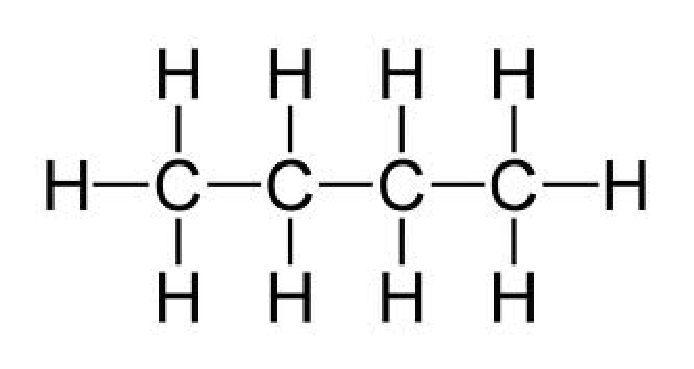
\includegraphics[width=4cm]{butane}\hspace*{1cm}
\includegraphics[width=4cm]{isobutane}
\end{center}
\caption{Butane (on the left) and isobutane (on the right).}
\label{f:isomer}
\end{figure}
We remark that different atoms\index{atom} have different properties:
carbons,\index{carbon} for example, can be incident to exactly 4
edges, whilst hydrogens\index{hydrogen}, can only be incident to
exactly 1 edge\index{edge} (we also say that carbons have {\it
  valence}\index{valence} 4 and hydrogens have valence 1).

Some graph structures of specific properties are also known,
e.g.~paraffins\index{paraffin} are known to have tree-like bond
relations. Thus, a natural question arose: how many different isomers
with certain graph properties shared a same chemical
formula?\index{chemical formula} From a purely formal (rather than
chemical) point of view, listing all paraffins is equivalent to
listing all trees with a given number $n$ of
vertices.\index{tree!listing} This can be done by listing all Pr\"ufer
sequences and transforming them to the corresponding trees (see
Sect.~\ref{s:tree:pruferseq}).

\begin{ex}
Devise and implement an algorithm for listing all trees of $n$ carbons
and hydrogens. Make sure the corresponding valences are
respected. List all trees of carbons and hydrogens have 4,5 and 6
vertices.
\end{ex}

\subsection{Trees and languages}
\label{s:tree:language}
A language\index{language} can be either formal\index{language!formal}
or natural.\index{language!natural} Formal languages follow a
well-defined set of precise syntactical rules\index{rule!syntactical}
for producing valid sentences.\index{sentence!valid} Programming
languages,\index{language!programming} for example, are formal
languages (see Sect.~\ref{s:computation:languages}). Moreover, in a
formal language each valid sentence can have at most one
meaning.\index{language!meaning}

Languages that are not formal are called natural, e.g.~English and
French are natural languages. The validity of a sentence in a natural
language is a fuzzy notion. It is clear that certain sentences are
invalid (e.g.~``me you drink I dog"), and it is also clear that
certain sentences are valid (e.g.~``my name is Leo"), but there are
sentences that may be valid or invalid depending on a context which
goes beyond the language itself (e.g.~``would you please\dots no,
leave it" has an auxiliary verb --- ``would" --- that lacks a main
verb; and yet, in a context of hesitation, it makes sense), or other
sentences that are syntactically ambiguous\index{sentence!ambiguous}
(e.g.~``Ibis redibis non morieris in bellum", which can be translated
as ``you will go and come back, you won't die in war" as well as ``you
will go but not come back, and die in war").

\subsubsection{Trees and recursion}
Trees are the best type of structure to model a recursive
behaviour. Each recursive action will refer to itself (or variations
of itself) one or more times during its existence. This creates a
hierarchy of actions, related by reference, which is best represented
as a tree.
\begin{eg}
In the example below, an action $A$ is declined into five variants
$A_1,\ldots,A_5$: $A_1$ refers to $A_3$ and $A_2$, which itself refers
to $A_4$ and $A_5$.
\begin{center}
\begin{tikzpicture}[scale=1]
\Tree [.$A_1$ [.$A_2$ $A_4$ $A_5$ ] $A_3$ ]
\end{tikzpicture} 
\end{center}
\end{eg}

\subsubsection{Syntax of formal languages}\index{language!formal!syntax}
A sentence of a formal language is defined to be valid in a
constructive way. Consider for example the formal language of all
mathematical expressions\index{expression!mathematical} consisting of
constants\index{constant} $c\in\mathbb{R}$, variable
symbols\index{variable} $x_i$ for any $i\in\mathbb{N}$, the binary
operators\index{operator!binary} sum, difference, multiplication,
division, power, and the unary operators\index{operator!unary} unary
minus, logarithm and exponential.  Valid sentences in this language
are called expressions.

\paragraph{Construction of valid sentences}
We define expressions as follows:
\begin{itemize}
\item constants and variable symbols are expressions,
\item for any two expressions $f$ and $g$, $f+g,f-g,fg,f/g,f^g$ are expressions,
\item for any expression $f$, $-f,\log(f),\exp(f)$ are expressions,
\item no other sentence, aside from those obtained by the rules above,
  is an expression.
\end{itemize}
The concept of expression is used recursively to construct ever more
complicated expressions. The last rule bars any other sentence from
being valid.

\paragraph{Recognition of valid sentences}
Now suppose we are given a sentence, and we have to decide whether it
is an expression\index{expression} or not. If we are able to ``break
it down" into sub-expressions so as to obtain the recursive
process\index{recursion} that led to its construction, then it is
valid, otherwise, because formal languages are not
ambiguous,\index{ambiguous} it is not. Accordingly, we write the rules
above in a slightly different form.
\begin{itemize}
\item an expression is either a term, or a sum of an expression with a
  term, or a difference of terms
\item a term is either a power, or a multiplication of a term by a
  power, or a division of powers
\item a power is either a function, or a function to the power of a
  function
\item a function is either a leaf,\index{leaf} or the negative of an
  expression, or the logarithm or exponential of an expression, or
  simply an expression within brackets
\item a leaf is either a constant\index{constant} or a variable
  symbol.\index{variable!symbol}
\end{itemize}
Here, the names {\it term}, {\it power}, {\it function}, {\it leaf}
denote a hierarchy level in the recursive application of our validity
verification method. Given a character string containing a sentence,
we try and match the rules above, starting from operators of lowest
precedence\index{operator!precedence} (sums and differences), to those
of highest precedence (unary operators). The set of rules above are
the {\it grammar}\index{grammar!formal} of the formal language of
mathematical expressions. It is written succinctly as follows:
\begin{equation}
\left.\begin{array}{rcl}
  {\tt e} & : & {\tt t} \quad|\quad {\tt e} + {\tt t} \quad|\quad {\tt
    t} - {\tt t} \\ 
  {\tt t} & : & {\tt p} \quad|\quad {\tt t} \times {\tt p} \quad|\quad
  {\tt p}\div {\tt p} \\ 
  {\tt p} & : & {\tt f} \quad|\quad {\tt f}\uparrow{\tt f} \\ 
  {\tt f} & : & {\tt l} \quad|\quad -({\tt e}) \quad|\quad \log({\tt
    e}) \quad|\quad \exp({\tt e}) \quad|\quad ({\tt e}) \\ 
  {\tt l} & : & x_i \quad (1\le i\le n) \quad|\quad c  \quad (c\in\mathbb{R}).
\end{array} \right\}
\label{eq:grammar}
\end{equation}
where the {\it grammar labels}\index{grammar!label} {\tt e}, {\tt t},
{\tt p}, {\tt f}, {\tt l} obviously denote expression, term, power,
function and leaf.\index{leaf}

The process of recognizing the validity of a given sentence, also
called {\it parsing},\index{parsing} naturally yields a tree (called
the {\it derivation tree}\index{tree!derivation} or {\it parse
  tree}\index{tree!parse}), whose vertices are labelled by the grammar
labels. The derivation tree subsumes the so-called {\it expression
  tree},\index{tree!expression}\index{expression!tree} which relates
operators\index{operator} and operands,\index{operand} as shown in
Example \ref{eg:derivtree}.

\begin{eg}
\label{eg:derivtree}
Consider the expression $x_1(x_1+x_2)$. The whole expression is
initially parsed as a term, which is parsed as a multiplication of two
terms: the first, $x_1$, is parsed as a term, then as a power, then as
a function, and finally as a leaf. The second, $(x_1+x_2)$, is parsed
as a power, then as a function, then, shedding its brackets, as an
expression, which is itself parsed as a sum of an expression and a
term, and so on. The derivation tree is shown below as a directed tree
with dashed arcs. The subsumed expression tree is shown as a directed
tree with whole arcs.
\begin{center}
\psfrag{E}{{\tt e}}
\psfrag{T}{{\tt t}}
\psfrag{P}{{\tt p}}
\psfrag{F}{{\tt f}}
\psfrag{L}{{\tt l}}
\psfrag{x1}{$x_1$}
\psfrag{x2}{$x_2$}
\psfrag{*}{$\times$}
\psfrag{+}{$+$}
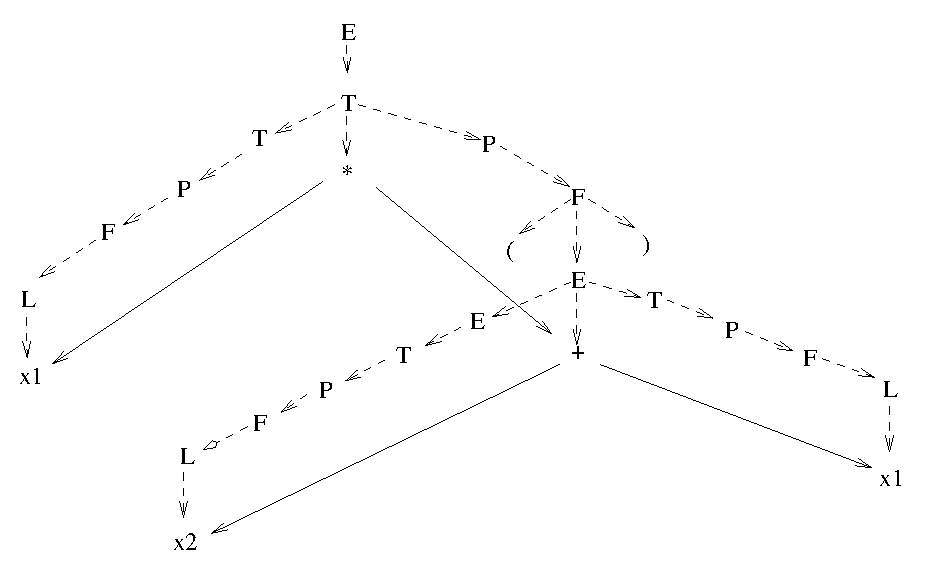
\includegraphics[width=10cm]{derivationtree}
\end{center}
\end{eg}

We remark that the name ``leaf" assigned to the grammar label {\tt l}
now makes sense, insofar as leaves label the leaf vertices of the
derivation tree.

\subsubsection{Semantics of formal languages}\index{language!formal!semantics}\index{semantics}
Although this fails to even begin to skim the surface of a very
complicated story, the semantics\index{semantics} (read: ``meaning")
of a formal (valid) sentence\index{sentence!meaning} is an assignment
of certain entities to the variable
symbols\index{variable!symbol}. The entities are usually
sets\index{set}, or numbers, or other mathematical abstractions. But
this need not be so. Rudolf Carnap\index{Carnap, R.} defined formal
languages in several scientific fields, including physics and
chemistry. In fact, alternative semantics allow a formal system to
describe a reality other than mathematical.

\subsubsection{Syntax of natural
  languages}\index{language!natural!syntax}\index{syntax}
\label{s:tree:language:syntnat}
Noam Chomsky\index{Chomsky, N.}, in \cite{chomsky}, attempted to
extend the use of derivation trees to parse natural language
sentences, as shown in Fig.~\ref{f:chomsky}.
\begin{figure}[!ht]
\begin{center}
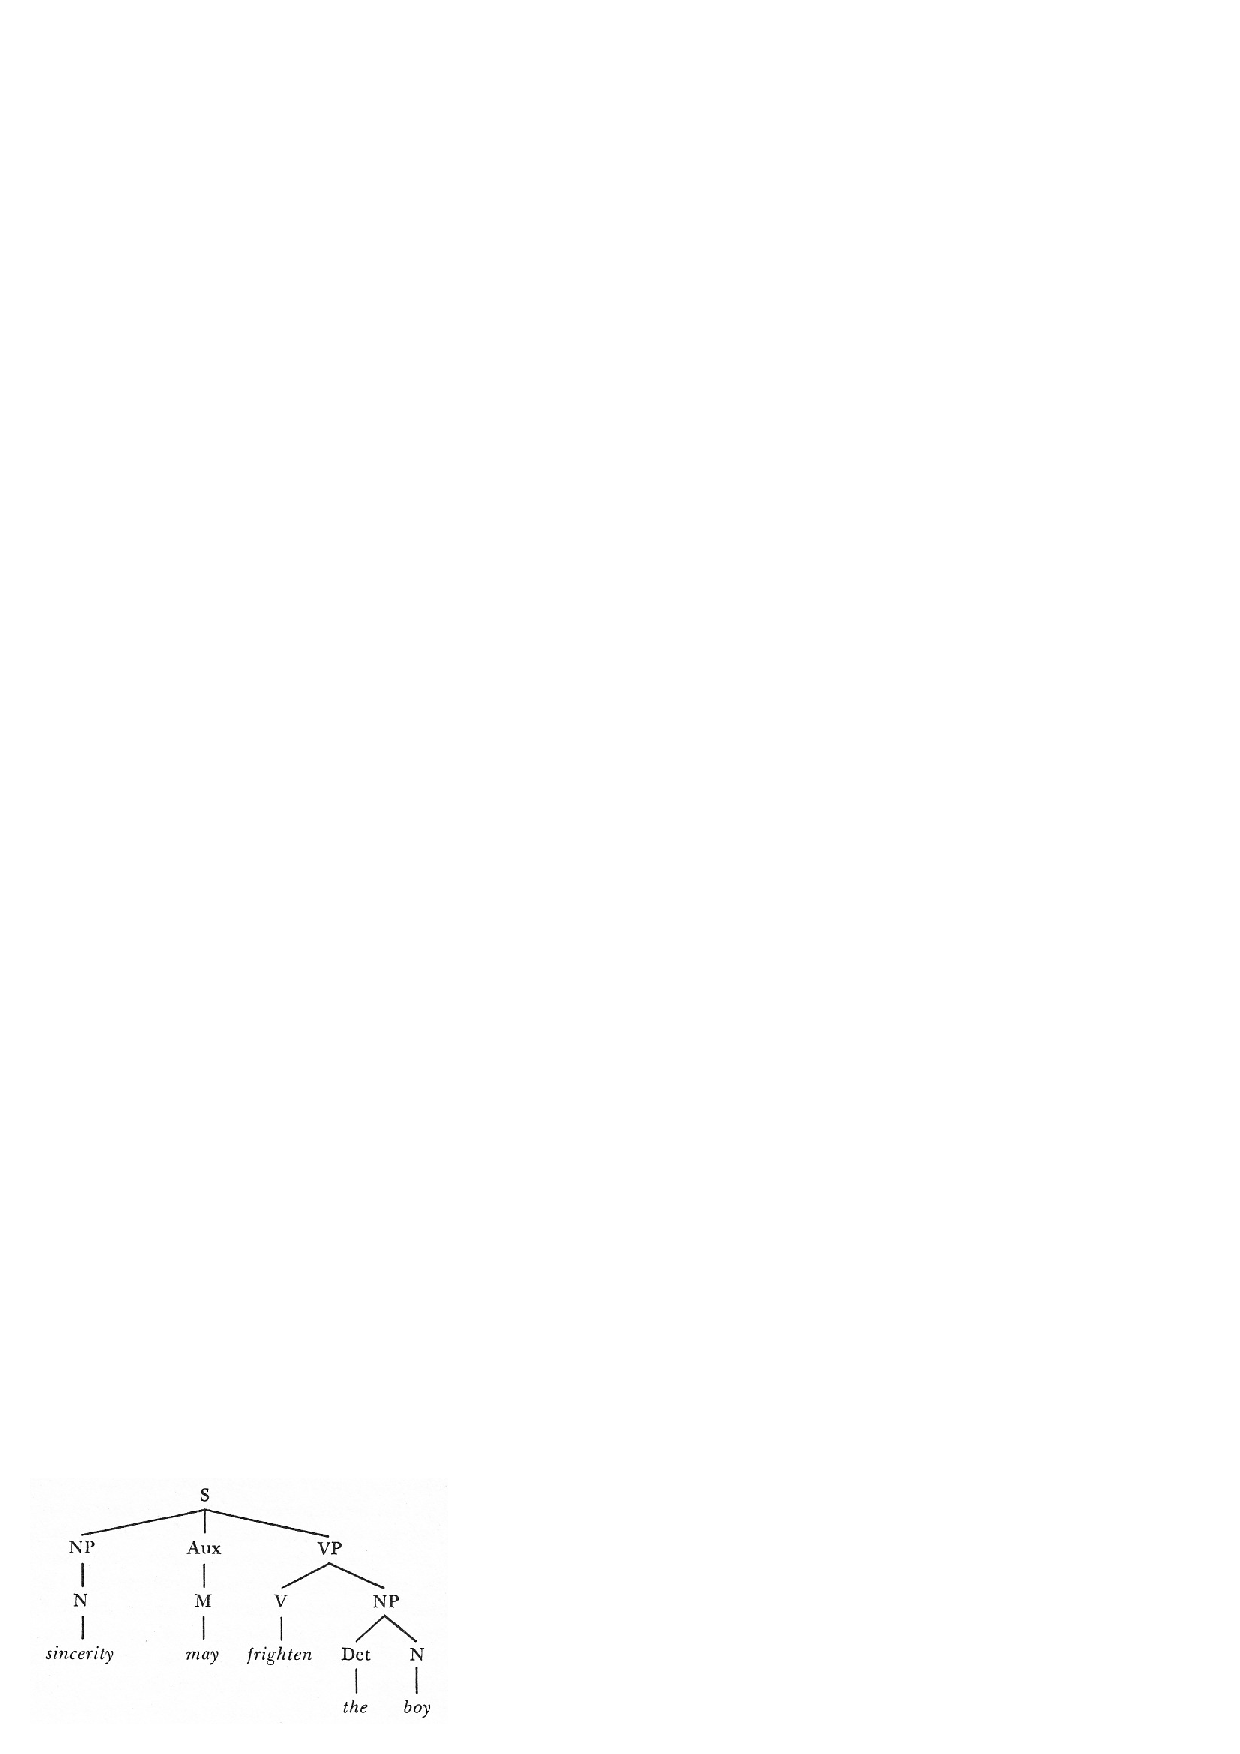
\includegraphics[width=7.5cm]{chomsky}
\end{center}
\caption{A derivation tree proposed by Chomsky \cite[p.~65]{chomsky}
  for the sentence ``sincerity may frighten the boy".}
\label{f:chomsky}
\end{figure}

\begin{eg}
The sentence (S) ``sincerity may frighten the boy" in
Fig.~\ref{f:chomsky} is parsed in the noun phrase (NP), the auxiliary
(Aux) and the verb phrase (VP). Recursively, NP is simply parsed into
a noun (N); Aux into a modal (M), and VP into a verb (V) and a new
noun phrase (VP), which is itself parsed into a determiative article
(Det) and a noun (N).
\end{eg}

\begin{ex}
Try writing a natural language grammar for a subset of a natural
language of your choice.
\end{ex}

\subsubsection{Semantics of natural languages}\index{language!natural!semantics}\index{semantics}
Richard Montague\index{Montague, R.}, a student of Alfred
Tarski's,\index{Tarski, A.} borrowed the tools of axiomatic set
theory, especially recursion, to address the problem of ambiguity in
natural languages \cite{montague}. An ambiguous sentence is one that
has multiple derivation trees, see Example \ref{eg:ambiguous}.

\begin{eg}
\label{eg:ambiguous}
Consider the latin sentence {\it ibis redibis non morieris in bellum}
cited at the beginning of Sect.~\ref{s:tree:language}. It has two
different parse trees:
\begin{center}
\begin{tikzpicture}
\Tree [.S [.VP [.V {\it ibis} ] ] [.VP [.V {\it redibis} ] ] [.VP [.Neg {\it non} ] [.V {\it morieris} ] [.Place {\it in} {\it bellum} ] ] ]
\end{tikzpicture}
\hspace*{1cm}
\begin{tikzpicture}
\Tree [.S [.VP [.V {\it ibis} ] ] [.VP [.V {\it redibis} ] [.Neg {\it non} ] ] [.VP [.V {\it morieris} ] [.Place {\it in} {\it bellum} ] ] ]
\end{tikzpicture}
\end{center}
By assigning the common latin meanings to the leaves {\it ibis},
{\it redibis}, {\it non}, {\it morieris}, {\it in}, {\it bellum},
there follow two different interpretations of these two trees. We
remark that the Latin syntax makes the {\it tu} (you) noun phrase
implicit in the verb phrases; and each VP in a single sentence is
linked by the other by an implicit {\it et} (and).
\end{eg}
From a syntactical point of view, Montague devised ways to modify
natural grammars so that ambiguities would be restricted to leaves. He
obtained this by allowing leaves to stand for whole sets of
(ambiguous) subtrees. For a given ambiguous sentence, this somehow
yielded unique grammar trees ``modulo ambiguity".

Some ambiguous sentences resisted this approach. To deal with them,
Montague postulated the existence of appropriate semantics, so that
the meaning assigned to the leaves would make at most one derivation
tree true, and all the other ambiguous ones false. This is similar to
the Sybilla telling the soldier ``ibis redibis non morieris in bello"
{\it after} the soldier was safely back from the war, rather than
before: by its very presence, the soldier made one of the two
ambiguous trees yield a false sentence, and the other a true one. In
very poor words, this amounts to the mathematical formalization of the
concept of understanding a potentially ambiguous sentence by a given
context.

\subsection{Trees in networks}
\label{s:tree:network}
A {\it network}\index{network} is simply another name for ``graph",
used in certain engineering and scientific communities.

\subsubsection{Commodity networks}
\label{s:tree:network:commodity}
Consider a set of geographical sites that need to be connected in
order to exchange information,\index{information!exchange} or
electrical power,\index{power} or any other
commodity.\index{commodity} Any site can serve as proxy to
route\index{route} the commodity between any site pair. Laying a
connection infrastructure, be it eletrical or optical wires, or pipes,
incurs a cost:\index{cost} this could be unitary\index{cost!unitary}
(each communication link has a fixed cost), or proportional to the
length of each pairwise segment. We initially consider the set of
potential links\index{link} between pairs of sites that can be
geographically linked, and model this as a graph $G=(V,E)$, where $V$
is the set of sites and $E$ the set of potential links (such a graph
is also known as a {\it network}\index{network}). We want to find a
subgraph\index{subgraph} of $G$ that offers point-to-point
connectivity\index{connectivity} at minimum cost, while serving all
sites. Since all costs\index{cost!nonnegative} are nonnegative, this
is a minimally connected subgraph\index{subgraph!minimally connected}
of $G$, which, by Sections \ref{s:tree:spanning} and
\ref{s:tree:basicprop}, corresponds to a spanning
tree\index{tree!spanning} of $G$ of minimum
cost\index{tree!spanning!minimum cost} (see Fig.~\ref{f:sptree}).

\begin{figure}[!ht]
\begin{center}
\begin{minipage}{5cm}
\psfrag{v1}{$v_1$}
\psfrag{v2}{$v_2$}
\psfrag{v3}{$v_3$}
\psfrag{v4}{$v_4$}
\psfrag{1.3}{$1.3$}
\psfrag{1.4}{$1.4$}
\includegraphics[width=4cm]{spt1} 
\end{minipage}
\hspace*{1cm}
\begin{minipage}{5cm}
\psfrag{v1}{$v_1$}
\psfrag{v2}{$v_2$}
\psfrag{v3}{$v_3$}
\psfrag{v4}{$v_4$}
\psfrag{1.3}{$1.3$}
\psfrag{1.4}{$1.4$}
\includegraphics[width=4cm]{spt3}
\end{minipage}
\end{center}
\caption{A graph with its minimum spanning tree.}
\label{f:sptree}
\end{figure}

\subsubsection{Distance networks}
Spanning trees are also useful for storing compact encodings of
massive data sets. Consider for example a long list
$V=(v_1,\ldots,v_n)$ of long binary sequences
$v_i=(v_{i1},\ldots,v_{im})$ of the same length $m$.

First, we compute all {\it Hamming
  distances}\index{distance!Hamming}\index{Hamming} $h_{ij}$ between
every pair $\{v_i,v_j\}$, which we use to label the edges\index{edge}
of a complete graph\index{graph!complete} on $V$, also known as {\it
  distance network}.\index{network!distance} We remark that the
Hamming distance between two bit sequences of the same length is the
number of flips\index{flip} necessary to transform a sequence into the
other, e.g.~$01100$ and $00110$ have Hamming distance 2, since we must
flip the second and fourth bits to obtain a sequence from the other.

Netx, we find the minimum cost spanning tree $T$ in the distance
network, and enrich each edge $\{v_i,v_j\}$ in $T$ with the sequence
$K_{ij}=(k_1,\ldots,k_{h_{ij}})$ of element indices such that flipping
all $v_{ik_\ell}$, for $\ell\in\{1,\ldots,h_{ij}\}$, yields $v_j$ (and
vice versa: why?). This means that, if we store $v_i$, we only need to
store the sequence $K_{ij}$ in order to retrieve $v_j$. Since $K_{ij}$
is shorter than $v_j$, we gain in storage space.

Finally, we store the following information:
\begin{itemize}
\item any $v_0\in V$;
\item the tree $T$ with the edge information $(h_{ij},K_{ij})$ for
  each edge $\{v_i,v_j\}$.
\end{itemize}
This guarantees that every $v\in V$ can be reconstructed using $v_0$
and the information in $T$. Since $T$ has minimum cost, $\sum_{i,j}
|K_{ij}|$ is minimum, which means that this is the most compact
possible encoding of $V$.

\begin{eg}
Consider the following set $V$ of bit sequences:
\begin{center}
\begin{enumerate}
\item {\tt 011100011101}
\item {\tt 101101011001}
\item {\tt 110100111001}
\item {\tt 101001111101}
\item {\tt 100100111101}
\item {\tt 010101011100},
\end{enumerate}
\end{center}
with pairwise Hamming distance given by the following matrix (we only
report the upper right triangle, since the lower left is symmetric
(why?)
\begin{center}
\begin{tabular}{c|cccccc}
  & 1 & 2 & 3 & 4 & 5 & 6 \\ \hline
1 & 0 & 4 & 4 & 5 & 4 & 3 \\
2 & - & 0 & 4 & 3 & 4 & 5 \\
3 & - & - & 0 & 5 & 2 & 5 \\
4 & - & - & - & 0 & 3 & 6 \\
5 & - & - & - & - & 0 & 5 \\
6 & - & - & - & - & - & 0. 
\end{tabular}
\end{center}
The minimum spanning tree has cost 5:
\begin{center}
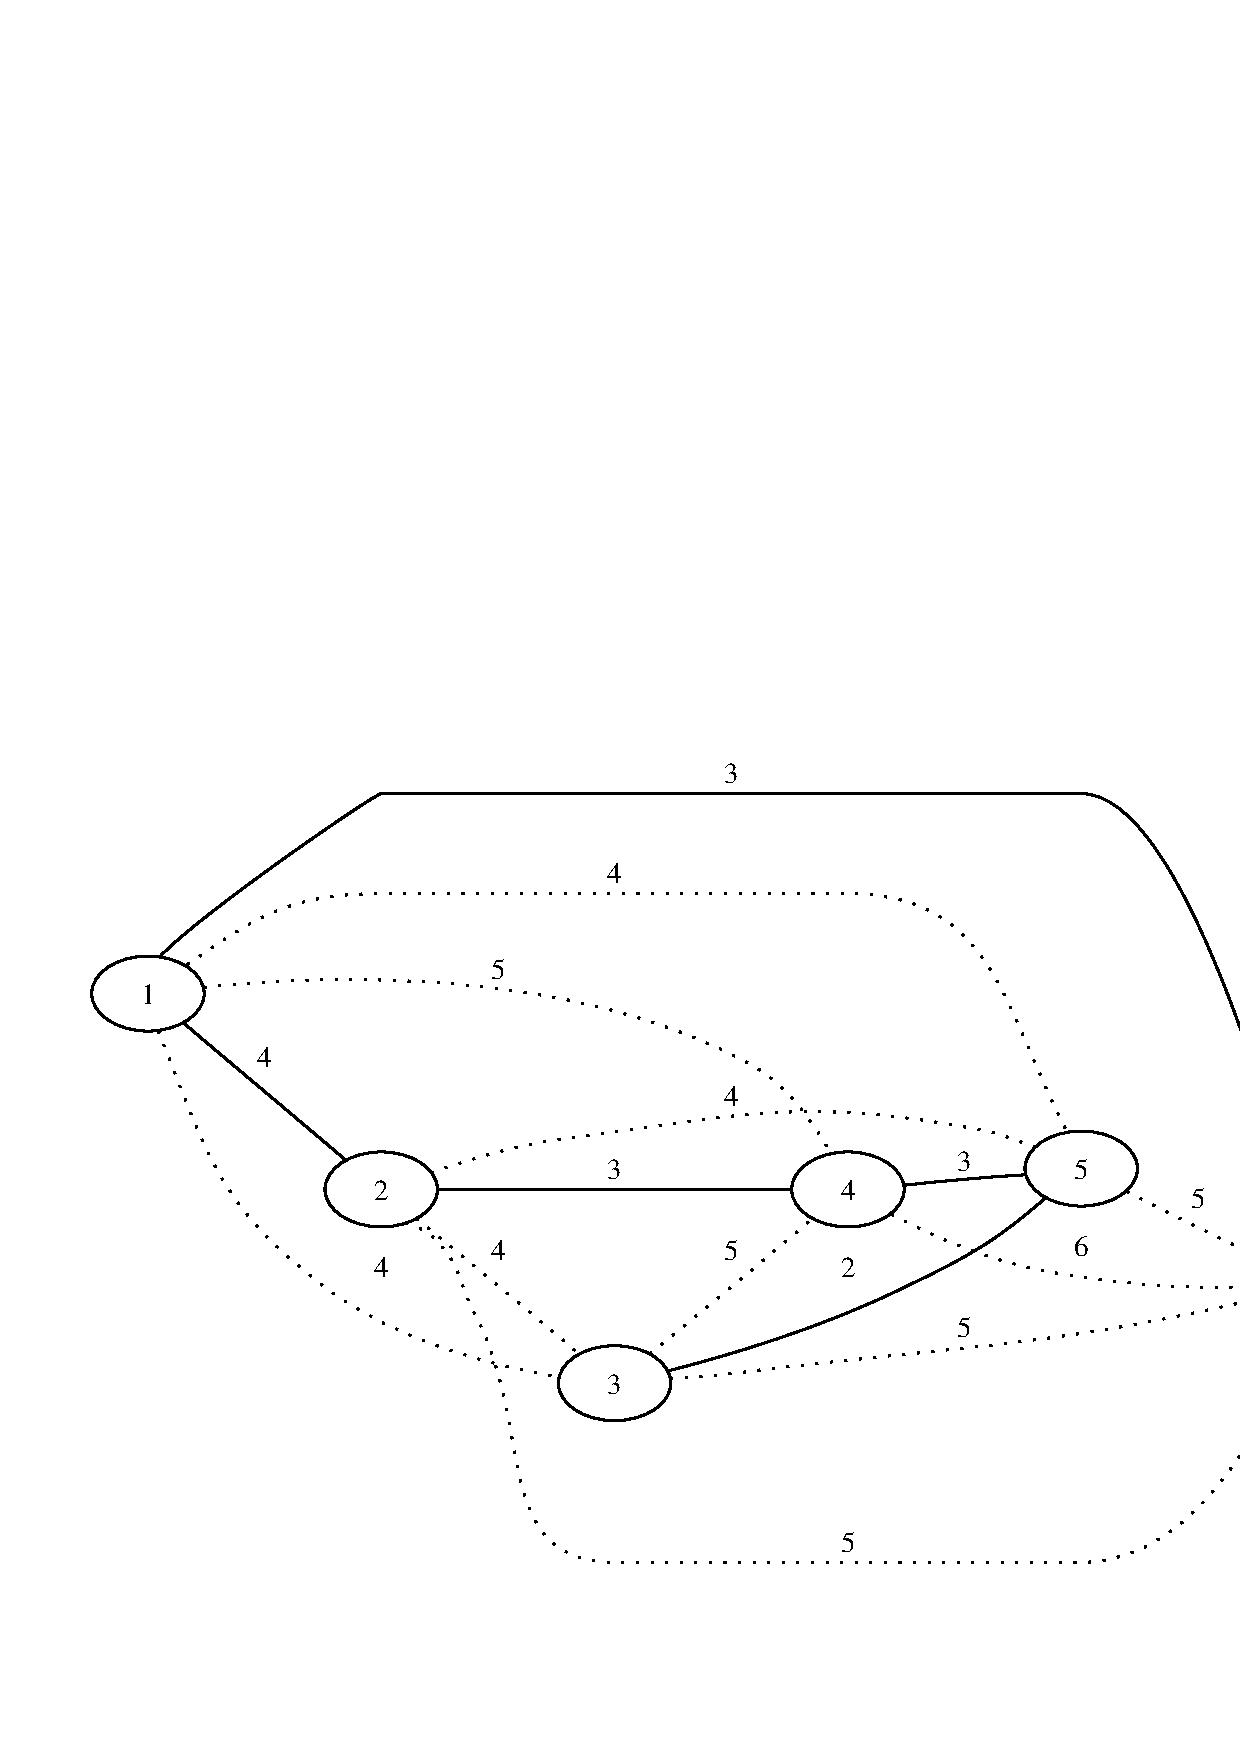
\includegraphics[width=10cm]{distnetsptree}
\end{center}
\end{eg}


%%%%%%%%%%%%%%%%%%%%%%%%%%%%%%%%%%%%%%%%%%%%%%%
%%%%%%%%%%%%%%%%% PART III %%%%%%%%%%%%%%%%%%%%
%%%%%%%%%%%%%%%%%%%%%%%%%%%%%%%%%%%%%%%%%%%%%%%

\part{Algorithms}
\label{p:alg}

%%%%%%%%%%%%%%%%% CHAPTER: RECURSION %%%%%%%%%%%%%%%%%%%%
\chapter{Recursive algorithms}
\label{c:recursion}

\begin{center}
\fbox{\begin{minipage}{13cm}{\small {\sc Abstract}.  
Motivations for using recursion. Recursion as a loop. Examples of
recursive algorithms (with some Java implementations): enumerating
permutations and the Hanoi tower. Recursion in logic: G\"odel's
incompleteness theorem.
}
\end{minipage}}
\end{center}

A recursive algorithm is one that includes one or more recursive
procedures.\index{procedure!recursive} A procedure is recursive if one
of its instructions is a call to itself. This may not sound so
convincing, except that procedures are implemented as functions in a
programming language, and hence take input arguments: a recursive
function call\index{function!call!recursive} will almost certainly
take a different set of argument values than the calling function
took. 

\section{Motivations}

\subsection{Proving program properties}
One of the main points in favour of using recursion is that it usually
makes it easy to prove that a recursive function actually does what it
is supposed to do. This is related to mathematical
induction:\index{induction!mathematical} it suffices to check that an
induction start and an induction step hold, and the property is proved
for all values of a certain discretely changing argument.

\begin{ex}
\label{ex:factorialrecursive}
Using mathematical induction, prove that the following
recursive\index{factorial!recursive} program computes $n!$. \\ 
{\bf function} $f(n)$ {\tt \{} \\ [-1em]
\begin{algorithmic}
\IF{$(n=0)$}
  \RETURN 1
\ENDIF
\RETURN $n\times f(n-1)$
\end{algorithmic} 
\vspace*{-1em}
{\tt \}}
\end{ex}

\subsection{Expressing certain procedures naturally}
Another strong point for recursion is that it allows to write certain
programs more ``naturally''. Try programming a computer to explore the
tree\index{tree} below so that it follows the vertices in the natural order
$1,2,3,4,5,6$.
\begin{center}
\begin{tikzpicture}
\Tree [.1 [.2 3 4 ] [.5 6 ] ]
\end{tikzpicture}
\end{center}
Notice that in this case the natural order arises from exploring the
tree depth-first, starting from vertex 1. This is called {\it
  depth-first search}\index{search!depth-first}\index{depth-first}
(DFS)\index{DFS} and will be discussed in later chapters.

\subsubsection{Encoding the tree}
Since a tree is a graph,\index{graph} we encode it using an adjacency
list\index{list!adjacency} (see
Sect.~\ref{s:linear:array:jagged:adjacencylist}) $A$, defined as
follows:
\begin{flushleft}
$A_1$: $A_{11}= 2$, $A_{12}=5$ \\
$A_2$: $A_{21}= 3$, $A_{22}=4$ \\
$A_{3}$: $\varnothing$ \\
$A_{4}$: $\varnothing$ \\
$A_5$: $A_{51}=6$ \\
$A_6$: $\varnothing$,
\end{flushleft}
so that $A_{ij}$ is the vertex label of the $j$-th child of vertex $i$
of the tree.

\subsubsection{A code with limited scope}
\label{s:recursion:limited}
A na\"{\i}f student might initially code something like:
\begin{center}
\begin{algorithmic}
\STATE $\mbox{\tt int\;}a=1$;
\STATE print $a$;
\FOR{$(\mbox{\tt int\;}z=1$ to $|A_{a}|)$} 
  \STATE $\mbox{\tt int\;}b=A_{az}$;
  \STATE print $b$;
  \FOR{$(\mbox{\tt int\;}y=1$ to $|A_{b}|)$}
    \STATE $\mbox{\tt int\;}c=A_{by}$;
    \STATE print $c$;
    \STATE \dots
  \ENDFOR
\ENDFOR
\end{algorithmic}
\end{center}
For the given tree, this might work. But change the tree, and the code
stops working: the number of loops\index{loop} depends on the number
of vertices, and it is ``hard-coded'' in the
pseudocode.\index{pseudocode} Ideally, our codes should work for all
similarly structured inputs,\index{input} in this case all trees.

\subsubsection{Algorithms and problems}
\label{s:recursion:motivation:natural:algprobs}
More formally, we recall that a problem is a set of inputs with
relative answers (see Sect.~\ref{s:computation:problem}); here, the
relevant decision problem is ``given a tree on $n$ vertices numbered
$1$ to $n$, does DFS exploration yield the order $1,\ldots,n$?'' The
possible inputs (also called {\it
  instances}\index{instance}\index{problem!instance} of the problem)
are the pairs $(n,T)$ where $n\in\mathbb{N}$ and $T$ is a tree on $n$
vertices. As was said in Sect.~\ref{s:computation:algorithm}, an
algorithm\index{algorithm} is supposed to be able to solve a problem
(i.e.~a whole infinite set of instances) rather than a single
instance, or a handful thereof, taking each individual instance as
input. So the code in Sect.~\ref{s:recursion:limited} is no good.

\subsubsection{Recursion saves the day}
\label{s:recursion:motivation:natural:save}
We can very naturally model the depth-first nature of the tree
exploration using recursion, by calling $f(1)$ where $f$ is the
function below.
\begin{flushleft}
{\bf function} $f(\mbox{\tt int\;}\ell)$ {\tt \{} \\ 
\begin{algorithmic}
  \STATE print $\ell$;
  \FOR{$(\mbox{\tt int\;}i=1$ to $|A_\ell|)$}
    \STATE $f(A_{\ell i})$;
  \ENDFOR
\end{algorithmic}
{\tt \}}
\end{flushleft}
If we trace the input argument $\ell$ to the function $f$ below, we
obtain the following function call
tree:\index{tree!function call}\index{function!call!tree} 
\begin{center}
\begin{tikzpicture}
\tikzset{level distance=1.5cm}
\Tree [.\fbox{$1$} [.\fbox{$A_{11}=2$} \fbox{$A_{21}=3$}
    \fbox{$A_{22}=4$} ] [.\fbox{$A_{12}=5$} \fbox{$A_{51}=6$} ] ]
\end{tikzpicture}
\end{center}
which, we remark in order to emphasize how naturally recursion can
model a DFS, is the same as the original input tree. 

\subsubsection{Back to iteration}
To those students who might think that recursion is necessary to
express certain types of programs, we explicitly say {\it this is not
  the case}! It suffices to introduce a stack\index{stack} and change
recursive calls back to their internal form (pushing\index{stack!push}
addresses\index{address} on the stack, and then
popping\index{stack!pop} them in order to jump back to the calling
functions, see Sect.~\ref{s:linear:stack:function}). Here are the
actions that the recursive algorithm of
Sect.~\ref{s:recursion:motivation:natural:save} performs on the given
tree.
\begin{enumerate}
\setlength{\parskip}{-0.5em}
\item $\ell=1$; print 1
\item $|A_1|=2$; $i=1$
\item call $f(A_{11}=2)$ [push $\ell=1$]
\item $\ell=2$; print 2
\item $|A_2|=2$; $i=1$ 
\item call $f(A_{21}=3)$ [push $\ell=2$]
\item $\ell=3$; print 3
\item $A_3=\varnothing$
\item return \hspace*{1.15cm} [pop $\ell=2$]
\item $|A_2|=2$; $i=2$
\item call $f(A_{22}=4)$ [push $\ell=2$]
\item $\ell=4$; print 4
\item $A_4=\varnothing$
\item return \hspace*{1.15cm} [pop $\ell=2$]
\item return \hspace*{1.15cm} [pop $\ell=1$]
\item $|A_1|=2$; $i=2$
\item call $f(A_{12}=5)$ [push $\ell=1$]
\item $\ell=5$; print 5
\item $|A_5|=1$; $i=1$
\item call $f(A_{51}=6)$ [push $\ell=5$]
\item $\ell=6$; print 6
\item $A_6=\varnothing$
\item return \hspace*{1.15cm} [pop $\ell=5$]
\item return \hspace*{1.15cm} [pop $\ell=1$]
\item return; end
\end{enumerate}

\begin{ex}
Write an iterative version of the recursive algorithm in
Sect.~\ref{s:recursion:motivation:natural:save}. Make sure it works on
every possible input.
\end{ex}

\section{Iteration and recursion}
Compare the following two codes:
\begin{center}
\begin{tabular}{|c|c|}\hline
\begin{minipage}{6cm}
\begin{algorithmic}
\WHILE{({\tt true})}
  \STATE print {\tt "Leo"};
\ENDWHILE
\end{algorithmic}
\end{minipage}
&
\begin{minipage}{6cm}
\vspace*{0.5em}
{\bf function} $f()$ {\tt \{} \\ [-1.2em]
\begin{algorithmic}
\STATE print {\tt "Leo"};
\STATE $f()$;
\end{algorithmic}
{\tt \}} \\ [0.3em] 
$f()$;
\par
\vspace*{0.5em}
\end{minipage} \\ \hline
\end{tabular}
\end{center}
Both programs yield the same infinite loop\index{loop!infinite} that
prints ``Leo'' on the screen without ever ending. The important point
is that recursion is a form of loop. Consider the following iterative
code for computing factorials:\index{factorial!iterative}
\begin{algorithmic}
\STATE input $n$;
\STATE $r=1$
\FOR{$(i=1$ to $n)$}
  \STATE $r=r\times i$
\ENDFOR
\STATE output $r$
\end{algorithmic}
and compare it with the recursive code in Exercise
\ref{ex:factorialrecursive}. Whereas the iterative code uses a loop
and assignments,\index{assignment} the recursive version only uses
recursion and nothing else. It might appear strange at first sight:
assignments are the way computers have to write to
memory\index{memory} --- can recursion stand in for memory? Not quite:
the subtle point is that recursion needs the OS\index{OS} to implement
function calls,\index{function!call} and that these, in turn, need a
stack to work (see Sect.~\ref{s:linear:stack:function}). Recursion is
implicitly making use of the stack memory during the {\tt return}
call: the returned values are stored on the stack, where the calling
function can access them. Insofar as universality\index{universality}
is concerned, machines with two stacks\index{stack} and an
alphabet\index{alphabet} of only one symbol are known to be
UTMs.\index{UTM}\index{Turing!machine!universal}

\subsection{Terminating the recursion}
The recursive procedure in the previous section did not terminate, as
the recursive function $f()$ called itself without arguments and
returned no value: all things being equal, there was no reason why the
next call should be any different from the previous. 

\begin{ex}
Prove formally, using mathematical
induction,\index{induction!mathematical} that a function $f()$ without
input arguments\index{input!argument} and return
values,\index{return!value} that just calls itself without doing
anything else, generates an infinite loop.\index{loop!infinite}
\end{ex}

Now consider a function $f(n)$, where $n\in\mathbb{N}$, and suppose
that the implementation of $f$ calls itself over a different argument
value, say $n-1$. Suppose also that, before calling itself, $f$
implements a test\index{test!termination} to ascertain that $n>0$,
whereas $f$ terminates without recursion if $n=0$. Then we can
conclude that $f$ does not yield an infinite loop.\index{loop!infinite}

\begin{ex}
Prove the last assertion formally.
\end{ex}

Typically, a general schema for recursive function implementations is
the following.
\begin{algorithmic}
\IF{$n$ is a ``base case''}
  \STATE compute $f(n)$ directly, do not recurse
\ELSE
  \STATE recurse on $f(i)$ with some $i<n$
\ENDIF
\end{algorithmic}
If we plot the values taken by $n$ against the level of
recursion\index{recursion!level} (this can be seen as stack
size),\index{stack!size} in order for $f$ to terminate we need a graph
like the one in Fig.~\ref{f:recterm} (left).
\begin{figure}[!ht]
\begin{center}
\includegraphics[width=7cm]{recterm1}
\includegraphics[width=7cm]{recterm2}
\end{center}
\caption{Input argument\index{input!argument} $n$ of a recursive
  procedure in function of recursion level.}
\label{f:recterm}
\end{figure}
Actually, it can be much crazier, it just suffices that it hits the
``base case'' in finite time (Fig.~\ref{f:recterm}, right).

\section{Listing permutations}
\label{s:recursion:permutation}
A {\it permutation}\index{permutation} of $n$ elements is a function
that maps an $n$-element sequence\index{sequence} to another
$n$-element sequence having the same elements as the first, but in a
different order.\index{order} More formally, a permutation is a
bijection from a finite set $V$ to itself, i.e.~an
automorphism\index{automorphism} on $V$.

In this section we show how recursion can help us list all possible
permutations of $n$ elements (for any given $n$).

\subsection{Some background material on permutations}
\label{s:recursion:permutation:notation}
We denote a permutation $\pi$ on the set
$[n]=\{1,\ldots,n\}$\index{$[n]$} by listing the
action\index{permutation!action}\index{action} of the permutation on
each element on $[n]$, for example:
\begin{equation*}
  \pi=\left(
  \begin{array}{cccc} 1 & 2 & 3 & 4 \\ 2 & 3 & 4 & 1 \end{array}
      \right)
\end{equation*}
sends $1\to 2$, $2\to 3$, $3\to 4$ and $4\to 1$. 

Sometimes the first line of the permutation representation above is
skipped, and we only denote $\pi$ by the second line.

\subsubsection{Product of permutations}
The product\index{permutation!product} of $\pi$ by the permutation
$\sigma=\left({\scriptsize\begin{array}{cccc}1&2&3&4\\[-0.2em]4&3&2&1\end{array}}\right)$,
defined by applying $\sigma$ first and $\pi$ later, and denoted as
$\pi\sigma$, has the following effect:
\begin{eqnarray*}
  1\xrightarrow{\sigma} &4& \xrightarrow{\pi} 1 \\
  2\xrightarrow{\sigma} &3& \xrightarrow{\pi} 4 \\
  3\xrightarrow{\sigma} &2& \xrightarrow{\pi} 3 \\
  4\xrightarrow{\sigma} &1& \xrightarrow{\pi} 2, 
\end{eqnarray*}
i.e.~it is the permutation:
\begin{equation*}
  \pi\sigma=\left(
  \begin{array}{cccc} 1 & 2 & 3 & 4 \\ 1 & 4 & 3 & 2 \end{array}
      \right).
\end{equation*}
We remark that the product of permutations is a
composition\index{composition} of bijections.\index{bijection} Since
the composition of two bijections on the same set is another bijection
on that set, the product of two permutations is still a permutation.

\begin{ex}
Prove that the compositions of two bijections on $V$ is another
bijection on $V$.
\end{ex}

\subsubsection{Group structure}
We now take a more abstract look at the permutation product. This
product is a binary operator between permutations: mathematically
speaking, it maps pairs of permutations into another
permutation. Whenever a $k$-ary operator\index{operator!$k$-ary} maps
$V^k$ to a set $U\subseteq V$, we say that the operator is {\it
  closed}\index{operator!closed} or that the set $V$ is
closed\index{set!closed} with respect to that operator.

\begin{ex}
Proving that the product of permutations is
associative\index{product!associative} is easy but long (and, for me,
also tedious, since I already did this when I was a student): amuse
yourself and do it as an exercise.
\end{ex}

The identity of the permutation product is the permutation
$e=\left({\scriptsize\begin{array}{cccc}1&2&3&4\\[-0.2em]1&2&3&4\end{array}}\right)$,
and the inverse\index{permutation!inverse} of each permutation is
obtained by simply ``reversing the arrows'': if a permutation $\pi$
sends $i$ to $j$, then $\pi^{-1}$ sends $j$ to $i$. In other words,
this means that $\pi^{-1}$ sends $\pi(i)$ to $i$, and therefore that
$\pi^{-1}(\pi(i))=i$ for all $i\in[n]$, which implies that
$(\pi^{-1}\pi)(i)=i$, i.e.~that $\pi^{-1}\pi=e$. Thus, the set of
permutations of $n$ elements form a group\index{group} under the
permutation product. This group, called the {\it symmetric group of
  order $n$},\index{group!symmetric} is denoted by $S_n$.

\begin{ex}
\label{ex:Snsize}
Prove that $|S_n|=n!$.
\end{ex}

We remark that, by a theorem of Cayley's, any finite group is
isomorphic to a subgroup of $S_n$ for some $n$.

\subsubsection{Cycle notation}
\label{s:recursion:permutation:cycle}
A {\it cycle permutation} (or simply a {\it
  cycle})\index{permutation!cycle} is a permutation $\pi\in S_n$ with
a sequence $(v_1,\ldots,v_\ell)$ such that $\pi(v_i)=v_{i+1}$ for all
$i<ell$ and $\pi(v_\ell)=v_1$, and $\pi(v)=v$ for all other elements
$v\in V\smallsetminus\{v_1,\ldots,v_\ell\}$. Informally, the action of
$\pi$ on $V$ is described graphically in Fig.~\ref{fig:cycleperm} for
a case where $\ell=6$.
\begin{figure}[!ht]
\begin{center}
\begin{tikzpicture}
  \GraphInit[vstyle=Normal]
  \SetGraphUnit{2}
  \SetVertexMath
  \Vertices{circle}{v_1,v_2,v_3,v_4,v_5,v_6}
  \Edges[style={->,bend right}](v_1,v_2,v_3,v_4,v_5,v_6,v_1)
\end{tikzpicture}
\end{center}
\caption{The action of a cycle permutation.}
\label{fig:cycleperm}
\end{figure}

Cycles allow a more compact way of writing permutations. The
permutation
\begin{equation*}
  \pi=\left(
  \begin{array}{ccccccccc} 1 & 2 & 3 & 4 & 5 & 6 & 7 & 8 & 9\\ 
                           2 & 1 & 3 & 4 & 5 & 6 & 7 & 8 & 9
  \end{array}\right),
\end{equation*}
for example, only swaps\index{swap} 1 and 2 but still takes 9 pairs of
integers to write down: this is wasteful. But we can easily recognize
that $\pi$ is the cycle of length\index{cycle!length} 2 sending $1\to
2$ and $2\to 1$ and fixing all the other integers. We therefore write
$\pi$ more simply as $(1,2)$. In general, a cycle permutation sending
$\pi(v_i)$ to $v_{i+1}$ for all $i<\ell$ and $\pi(v_\ell)$ to $v_1$ is
denoted by its defining sequence $(v_1,\ldots,v_\ell)$.

Let $\pi=(v_1,\ldots,v_h)$ and $\sigma=(u_1,\ldots,u_k)$ be two
cycles. If these two cycles have no common elements, then their
product $\pi\sigma$ simply sends $v_i\to v_{i+1}$ for $i<h$, $u_i\to
u_{i+1}$ for $i<k$, $v_h\to v_1$ and $u_k\to u_1$. In other words, the
actions of $\pi$ and $\sigma$ are {\it
  disjoint}.\index{cycle!disjoint} 
\begin{ex}
Prove that, if $\pi,\sigma$ are two disjoint cycles, then 
$\pi\sigma=\sigma\pi$. Show that this property is lost in general if
the two cycles are not disjoint.
\end{ex}
We write the product of two disjoint cycles by simply juxtaposing the
two cycles, namely:
\begin{equation*}
  (v_1,\ldots,v_h)(u_1\ldots,u_k).
\end{equation*}

If the cycles $\pi,\sigma$ have some common elements, this analysis no
longer holds. For example, if $\pi=(1,2,3)$ and $\sigma=(1,2)$,
$\pi\sigma$ has the following effect (we apply $\sigma$ first and
$\pi$ later): $1\to 2\to 3$, $2\to 1\to 2$, $3\to 3\to 1$, which we
can write as $(1,3)$. What is true, however, is that any product of
non-disjoint cycles can be written as a product of (possibly
different) disjoint cycles, and moreover that any permutation can be
written as a product of disjoint cycles in a unique way apart from the
order of the factors (see \cite{clark}, p.~59).

\subsection{The inductive step}
We represent permutations by means of the second row of the $2\times
n$ matrix notation introduced in
Sect.~\ref{s:recursion:permutation:notation}.

The inductive step of our reasoning can be explained by means of
an example. Suppose $n=4$ and we are able to produce a complete list
of all permutations\index{permutation!list} of 3 elements:
\begin{equation*}
  (1,2,3), (1,3,2), (3,1,2), (3,2,1), (2,3,1), (2,1,3).
\end{equation*}
We write each of these permutations four times, and write the number 4
in every possible position, as follows.
\begin{equation*}
\begin{array}{cccc}
1 & 2 & 3 & {\bf 4} \\ 
1 & 2 & {\bf 4} & 3 \\ 
1 & {\bf 4} & 2 & 3 \\ 
{\bf 4} & 1 & 2 & 3 \\ [1em]
1 & 3 & 2 & {\bf 4} \\ 
1 & 3 & {\bf 4} & 2 \\ 
1 & {\bf 4} & 3 & 2 \\ 
{\bf 4} & 1 & 3 & 2 \\ [1em]
3 & 1 & 2 & {\bf 4} \\ 
3 & 1 & {\bf 4} & 2 \\ 
3 & {\bf 4} & 1 & 2 \\ 
{\bf 4} & 3 & 1 & 2 
\end{array}
\quad \quad
\begin{array}{cccc}
3 & 2 & 1 & {\bf 4} \\ 
3 & 2 & {\bf 4} & 1 \\ 
3 & {\bf 4} & 2 & 1 \\ 
{\bf 4} & 3 & 2 & 1 \\ [1em] 
2 & 3 & 1 & {\bf 4} \\ 
2 & 3 & {\bf 4} & 1 \\ 
2 & {\bf 4} & 3 & 1 \\ 
{\bf 4} & 2 & 3 & 1 \\ [1em] 
2 & 1 & 3 & {\bf 4} \\ 
2 & 1 & {\bf 4} & 3 \\ 
2 & {\bf 4} & 1 & 3 \\ 
{\bf 4} & 2 & 1 & 3 
\end{array}
\end{equation*}
We just obtained a complete list of all permutations of 4 elements.

\subsubsection{Generalizing the example to an integer $n$}
For a general $n$, if we have a complete list of permutations of $n-1$
elements, we have to write each of them $n$ times, then insert the
number $n$ at ever possible position (there are $n$ such positions) in
each block of $n$ equal permutations of $n-1$ elements. This exhausts
all the possibilities.

\begin{ex}
Reasoning by contradiction,\index{contradiction} prove the last
statement formally. 
\end{ex}

\subsubsection{The induction starts at 1}
Can we list all permutations of one element? Sure, here it goes:
$(1)$. This will be the base case of our recursive method.

\subsection{The algorithm}
\label{a:permlist}
The recursive function {\tt permutations}, given below, takes an
integer $n$ as input, and returns a set $L$ of all
permutations\index{permutation} of $n$ elements. It makes use of a
temporary set $L'$ containing all permutations of $n-1$ elements,
which is obtained by a recursive call\index{call!recursive} to {\tt
  permutations} with the argument set at $n-1$. The permutation $\pi$
is represented, as in Sect.~\ref{s:recursion:permutation:notation}, as a
sequence of integers $(\pi_1,\ldots,\pi_{n-1})$.

\begin{minipage}{10cm}
\begin{flushleft}
{\tt function permutations$(n)$ \{} \\
\begin{algorithmic}[1]
\IF{$(n=1)$}
  \STATE $L=\{(1)\}$;
\ELSE
  \STATE $L'=\mbox{\tt permutations}(n-1)$;\label{recstep}
  \STATE $L=\varnothing$;
  \FOR{$((\pi_1,\ldots,\pi_{n-1})\in L')$} \label{for1}
    \FOR{$(i\in \{1,\ldots,n\})$}
      \STATE
      $L\leftarrow L\cup\{(\pi_1,\ldots,\pi_{i-1},n,\pi_i,\ldots,\pi_{n-1})\}$;   
      \label{mainstep}
    \ENDFOR
  \ENDFOR
\ENDIF
\RETURN{$L$;}\label{retstep}
\end{algorithmic}
\vspace*{-0.1cm}
{\tt \}}
\end{flushleft}
\end{minipage}

\subsubsection{Data structures}
Since the number $n$ needs to be inserted at every possible position
in the sequence $\pi=(\pi_1,\ldots,\pi_{n-1})$, we choose a list for
storing $\pi$. As for the sets $L,L'$, since we know their sizes {\it
  a priori} (they have $n!$ and, respectively, $(n-1)!$ elements, by
Exercise \ref{ex:Snsize}), arrays\index{array} will suffice. For
$\pi$, on the other hand, since we need to add the element $n$ at
every possible position, we need linked lists.

\subsection{Java implementation}
Since permutations are in fact orders\index{orders} on sets with
elements in $\{1,\ldots,n\}$, the Java\index{Java} implementation of
the permutation listing algorithm\index{algorihm} is stored in the
file {\tt Orders.java}, containing only the class {\tt Orders}, which
also contains the {\tt main} method.

The file starts as usual, with comments\index{comment} and
imports.\index{import}
\begin{verbatim}
/*
  Name: Orders.java
  Purpose: list all permutations of n symbols
  Author: Leo Liberti
  Source: Java
  History: 28/8/11  work started
*/

import java.io.*;
import java.util.*;
import java.lang.*;
\end{verbatim}

\subsubsection{Class structure}
Here is the structure of the Java class: it consists of just three
static methods.\index{method!static} As mentioned above, we represent
permutations as linked lists\index{list!linked} and sets of
permutations as arrays.\index{array}
\begin{verbatim}
class Orders  {
    // used to print a list of integers in permutation format
    public static void printList(LinkedList<Integer> tl);

    // find all permutations (or orders) on n symbols 
    public static ArrayList<LinkedList<Integer> > orders(int n);

    // the main method
    public static void main(String[] args);
}
\end{verbatim}

The {\tt printList} method simply prints out a linked
list\index{list!linked} of integers: this is the representation of a
permutation, so this method actually prints a permutation to the
screen. 

The {\tt orders} method implements the recursive algorithm, and
returns a set $L$ of all permutations of $n$ elements. We need to
spend a paragraph about the difficult-looking type 
\begin{center}
{\tt ArrayList<LinkedList<Integer> >}. 
\end{center}
The {\tt ArrayList}\index{ArrayList@{\tt ArrayList}} type is a parametrizable
class that implements an array whose elements contain whatever
parameter type is given between angular brackets. In this case, the
parameter type is {\tt LinkedList<Integer>},\index{LinkedList@{\tt LinkedList}}
which is the same type taken by {\tt printList} to print out
permutations. So, all in all, 
\begin{center}
{\tt ArrayList<LinkedList<Integer> >} 
\end{center}
is the type of $L$ and $L'$ in the algorithm.

By the way, we are using {\tt Integer}s\index{Integer@{\tt Integer}} rather
than {\tt int}s\index{int@{\tt int}} because the former are passed by
reference\index{reference!passing}\index{passing!by reference} whilst
the latter are passed by value,\index{value!passing}\index{passing!by
  value} and you should always use ``reference
classes''\index{class!reference} (rather than elementary data
types)\index{type!elementary} as parameter types\index{type!parameter}
to parametrizable classes.\index{class!parametrizable}

\subsubsection{The {\tt main} method}
The point of entry\index{point of entry} reads an integer $n$ from the
first argument of the command line, then calls the recursive function
{\tt orders($n$)}, storing the resulting set in the {\tt ArrayList}
{\tt L} of {\tt LinkedList}s of {\tt Integer}s, then declares an {\tt
  Iterator}\index{Iterator@{\tt Iterator}} object to {\tt L}. 

{\tt Iterator}s behave like pointers,\index{pointer} insofar as their
{\tt next()}\index{Iterator@{\tt Iterator}!next@{\tt .next()}} method
will return the next object stored in the linear data
structure.\index{data!structure!linear} Their {\tt
  hasNext()}\index{Iterator@{\tt Iterator}!hasNext@{\tt .hasNext()}} method
allows testing whether the current reference\index{reference} being
held in the {\tt Iterator} points to the dummy object\index{object}
signaling the end of data structure.\index{data!structure} If this is
not the case, then the next reference\index{reference!next} is printed
on the screen.
\begin{verbatim}
    public static void main(String[] args) {
        
        // read n from cmd line
        int n = Integer.parseInt(args[0]);

        // first call to recursive function
        ArrayList<LinkedList<Integer> > L = orders(n);

        // loop on permutation list and print them all out
        Iterator<LinkedList<Integer> > ait = L.iterator();
        while(ait.hasNext()) {
            printList(ait.next());
            System.out.println();
        }
    }
\end{verbatim}

\subsubsection{The {\tt printList} method}
The {\tt printList} method also makes use of {\tt
  Iterator}s\index{Iterator@{\tt Iterator}} to print on the screen the list
representation of the permutations.
\begin{verbatim}
    public static void printList(LinkedList<Integer> tl) {
        Iterator<Integer> lit = tl.iterator();
        System.out.print("( ");
        while(lit.hasNext()) {
            System.out.print(lit.next() + " ");
        }
        System.out.print(")");
    }
\end{verbatim}

\subsubsection{The {\tt orders} method}
This is the implementation of the main recursive function. The
comments are in the code.
\begin{verbatim}
    public static ArrayList<LinkedList<Integer> > orders(int n) {

        // an array whose components are lists of integers 
        // the i-th component of the array contains the i-th permutation
        ArrayList<LinkedList<Integer> > L = 
            new ArrayList<LinkedList<Integer> >();

        if (n == 1) {
            // base case for recursion

            // when n=1, there is only one permutation: the identity (1)
            LinkedList<Integer> identity = new LinkedList<Integer>();
            identity.add(1);
            L.add(identity);

        } else {
            // recursive step

            // L' is the list of permutations on n-1 symbols
            ArrayList<LinkedList<Integer> > Lprime = orders(n-1);

            // loop on permutations of n-1 symbols
            Iterator<LinkedList<Integer> > ait = Lprime.iterator();
            while(ait.hasNext()) {

                // smallOrder is the next permutation in L'
                LinkedList<Integer> smallOrder = ait.next();

                // loop on permutation vector indices from last to first
                for(int i = n-1; i >= 0; i--) {

                    // insert symbol n at the i-th position in the smaller perm
                    smallOrder.add(i, (Integer) n);

                    // produce a new permutation as a copy of the old one
                    LinkedList<Integer> newOrder = 
                        new LinkedList<Integer>(smallOrder);

                    // add this new permutation to the list L
                    L.add(newOrder);

                    // remove symbol n from smaller permutation
                    smallOrder.remove(i);
                }
            }

        }
        return L;
    }

\end{verbatim}

\section{The Hanoi tower}
This is a great classic in the didactics of recursion; you'll find
hundreds, if not thousands, of different treatments either in print or
online, so we'll skim over this quickly.

The Hanoi towers\index{Hanoi towers} is a game which consists of three
poles, one of which holds a stack of $k$ concentric flat
cylinders\index{cylinder} with increasing radii\index{cylinder!radius}
(disks at the bottom of the stack have higher radius). The (unique)
player is challenged to move the stack, one cylinder at a time, from
one pole to another without ever changing the radius order (larger
cylinders below smaller ones) --- see Fig.~\ref{f:hanoi}.
\begin{figure}[!ht]
\begin{center}
\includegraphics[width=8cm]{tower_of_hanoi-diagram2}
\end{center}
\caption{The moves of the Hanoi towers game (picture taken online some
  time ago on Wikipedia --- I think).}
\label{f:hanoi}
\end{figure}

\subsection{Inductive step}
We shall number the poles from 1 to 3. In order to move $k$ cylinders
from pole 1 to pole 3, this is what we do:
\begin{enumerate}
\item move the topmost $k-1$ cylinders from pole 1 to pole 2
\item move the largest (bottom) cylinder from pole 1 to pole 3
\item move the $k-1$ discs from pole 2 to pole 3.
\end{enumerate}
Notice that in order to move $k$ cylinders, we move $k-1$ cylinders
twice, and move just one (the largest) cylinder from a pole to another
(free) pole. This solution seems to be good, as long as we know how to
move $k-1$ cylinders. 

We also remark that the steps involving the movement of $k-1$ cylinders
present no fundamental difference, aside from size, with moving $k$
cylinders. Since we are leaving the largest cylinder fixed, it is
never problematic: it is the largest, and it is at the bottom.

\subsection{Base case}
Our recursion base case is to deal with the case where $k=1$, i.e.~the
stack only consists of one cylinder. This is easy: simply move it from
pole 1 to pole 3, since there are no other complicating cylinders.

\begin{ex}
Is the Hanoi tower game harder or easier if we add poles?
\end{ex}

\subsection{Java implementation}
The Java\index{Hanoi towers!Java} implementation of the Hanoi tower
game is really simple. We hold a single {\tt Hanoi} class in the file
{\tt Hanoi.java}, which starts with the usual comments\index{comment}
and imports.\index{import} The {\tt Hanoi} class only consists of two
static methods: {\tt move(int from, int to, int $k$)}, which moves $k$
cylinders from pole {\tt from} to pole {\tt to}; and {\tt main}.

\begin{verbatim}
    // move "cylinders" cylinders from stack "from" to stack "to"
    public static void move(int from, int to, int k) {
        if (k == 1) {
            // base case for recursion
           System.out.println("move upper cyl. on stack "+from+" to stack "+to);
        } else {
            // recursive step
            
            // computing the index of the other stack 
            // (which is neither "from" nor "to")
            int other = 6 - (from + to);
            
            // first move k-1 cylinders from "from" to "other"
            move(from, other, k-1);

            // now move one cylinder from "from" to "to"
            move(from, to, 1);

            // finally move k-1 cylinders from "other" to "to"
            move(other, to, k-1);
        }
    }
\end{verbatim}

\begin{ex}
Prove that if $i\not=j\in\{1,2,3\}$, then $h=6-(i+j)$ is such that 
$\{i,j,h\}=\{1,2,3\}$.
\end{ex}

The {\tt main} method reads the number of cylinders in the initial
stack from the command line.
\begin{verbatim}
    public static void main(String[] args) {
        // read number of cylinders to move from cmd line
        String theArg = args[0];
        int cylinders = Integer.parseInt(theArg);

        // move these cylinders from stack 1 to stack 3
        move(1,3,cylinders);
    }
\end{verbatim}

\section{Recursion in logic}
Most of axiomatic set theory is built on recursive principles. One
starts with very elementary notions, such as the empty set, and
recursively applies simple operators and modifiers, to build ever more
complex structures. Infinities of different ordinality and cardinality
are treated using transfinite recursion \cite{kunen}.

In this section, I shall try to give you a very simplified, schematic
and partial view of what is possibly the most famous theorem in
mathematics: G\"odel's\index{G\"odel, K.} incompleteness
theorem.\index{G\"odel!incompleteness theorem}

\subsection{Definitions}
{\it Axioms}\index{axiom} are given sentences (of a formal language)
that define certain abstract entities (in our case, we require axioms
to describe at least the nonnegative integers). Axioms are true by
definition. The notation $\Phi\vdash\psi$ indicates that sentence
$\psi$ is a logical consequence of sentences in set $\Phi$. The
logical rules implicated in $\Phi\vdash\psi$ are required to be
carried out by a computer. Let $A$ be a set of axioms sufficient to
define integer arithmetic (e.g.~Peano's\index{Peano, G.}
Axioms).\index{Peano!axioms} A {\it theory}\index{theory} is a set
$T\supseteq A$ of sentences such that $A\vdash\phi$ for each $\phi\in
T$.
\begin{itemize}
\item A theory is {\it consistent}\index{theory!consistent} when it
  does not contain pairs of contradictory sentences $\phi,\neg\phi$.
\item A theory is {\it complete}\index{theory!complete} when every
  true statement expressible in the language is also in the theory.
\end{itemize}
Notice that there is a distinction between truth and logical
consequence: a sentence might be true although we may not be able to
prove it. This was the situation with Fermat's\index{Fermat} last
theorem until A.~Wiles\index{Wiles, A.} found a proof. Completeness
essentially asks a theory that it should prove every true statement.

\subsection{G\"odel's theorem}
\label{s:recursion:goedel}
It was Hilbert's\index{Hilbert, D.} dream to prove that a set of
axioms powerful enough to do integer arithmetic in would be both
consistent and complete, i.e.~all proofs could be derived
computationally for all and only for true
sentences. G\"odel\index{G\"odel, K.} shattered Hilbert's dream,
showing that no axiomatic system for integer arithmetic can ever be
both consistent and complete.

\subsection{The beautiful and easy part of the proof}
If $T$ is inconsistent,\index{theory!inconsistent} then every valid
sentence of the language, be it true or false, can be proved (can you
show this to be the case?). So we assume $T$ is consistent and aim to
show that there exists a true sentence not in $T$. Consider the
sentence $\gamma$, defined recursively as $T\neg\vdash\gamma$. In
natural language, $\gamma$ states ``I cannot be proved in $T$''.

By the law of the excluded middle, exactly one sentence in the set
$\{\gamma,\neg\gamma\}$ is true, and the other is false. We aim to
prove that neither is in $T$: this way it does not matter which is
true and which is false, at least one true sentence of the language
will fail to be in $T$.

We ask the following questions.
\begin{itemize}
\item Is $\gamma\in T$? If so, then $T\vdash\gamma$, which means that
  $T\vdash(T\not\vdash\gamma)$, i.e.~$T\not\vdash\gamma$,
  i.e.~$\gamma\not\in T$. This is a contradiction.
\item Is $(\neg\gamma)\in T$? If so, then $T\vdash\neg\gamma$,
  i.e.~$T\vdash\neg(T\not\vdash\gamma)$, that is
  $T\vdash(T\vdash\gamma)$, thus $T\vdash\gamma$. In other words,
  assuming $T\vdash\neg\gamma$ leads to $T\vdash\gamma$, which implies
  that $T$ is inconsistent. This is a contradiction, as we had assumed
  $T$ to be consistent.
\end{itemize}
We can only conclude that $T$ must be incomplete.

\subsection{The other part of the proof}
It is not immediately evident that the recursive definition
$T\neg\vdash\gamma$ has a ``base case''. The most difficult part of
G\"odel's proof is to encode all the logic he needed for his argument
within nonnegative integers. In particular, he was able to provide a
``finiteness proof'' for his recursive definition. This is very
technical, and we shall cowardly eschew it here. However, if you feel
up to a {\it really hard task}, 
\begin{ex}
Provide a formal proof of G\"odel's theorem.
\end{ex}
This has something to do with mapping all valid sentences to
nonnegative integers bijectively, and showing that there exists an
integer that maps back to $\gamma$. Of course you are free to read
G\"odel's original proof (bordering on the incomprehensible) as well
as any of the dozens of books (technical and otherwise) published
about this matter.

\subsection{A natural language interpretation}
Let us go back to $\gamma$, which was translated above to the natural
language sentence ``I cannot be proved in $T$''. The easy part of
G\"odel's proof is as follows. Prove ``I cannot be proved'': if you
can, what cannot be proved is proved, which is a contradiction. So
prove ``it is not true that I cannot be proved''. If you can, then
``I'' can be replaced by what it stands for, i.e.~``I cannot be
proved'': you then just proved that ``it is not true that `I cannot be
proved' cannot be proved'', which is the same as ``it is true that `I
cannot be proved' can be proved'' (we removed the double negation),
i.e.~`I cannot be proved' can be proved, which is again a
contradiction. This is why neither $\gamma$ nor its converse can be
proved in $T$, which is the reason why $T$ must be incomplete.

%%%%%%%%%%%%%%%%% CHAPTER: GRAPH EXPLORATION %%%%%%%%%%%%%%%%%%%%
\chapter{Graph searching and traversal}
\label{c:graphalg}

\begin{center}
\fbox{\begin{minipage}{13cm}{\small {\sc Abstract}.  
How to efficiently visit all vertices in a graph: breadth-first
search, depth-first search, and Prim's algorithm (with applications).
}
\end{minipage}}
\end{center}


In this chapter we shall present and discuss some basic (and
efficient) algorithms that explore, search and examine vertices and
edges in graphs.\index{graph!problem}

\section{Graph scanning}
\label{s:graphalg:gphscn}
A common task when solving problems on graphs is to visit all the
vertices: this may be a precondition for verifying some claim over the
graph vertices, or spawn actions on every vertex. The technical term
is {\it scanning} the vertices\index{vertex!scanning}\index{scanning}
of a graph (or the nodes\index{node!scanning} of a digraph), starting
from a given vertex (or node) $s$. 

\subsection{The {\sc Graph Scanning} algorithm}
Consider the following {\sc Graph Scanning}\index{graph scanning@{\sc
    Graph Scanning}} algorithm. It scans vertices (then puts them in a
set $R$), and examines vertices from a set $Q$.
\begin{algorithmic}[1]
\REQUIRE $G=(V,E)$, $s\in V$, $R=\{s\}$, $Q=\{s\}$
\WHILE{$Q\not=\varnothing$}
  \STATE choose $v\in Q$ {\tt // $v$ is scanned} \label{gs2}
  \STATE $Q\leftarrow Q\smallsetminus\{v\}$ \label{gs7}
  \FOR{$w\in N(v)\smallsetminus R$} \label{gs3}
    \STATE $R\leftarrow R\cup\{w\}$ \label{gs4}
    \STATE $Q\leftarrow Q\cup\{w\}$ \label{gs5}
  \ENDFOR
\ENDWHILE
\end{algorithmic}
While there remain vertices in $Q$, we pick one, say $v$, and explore
the vertices of its star $N(v)$ (or outgoing star $N^+(v)$ in case of
a digraph) that are still unscanned. We mark these as ``scanned'' by
putting them in $R$, and also put them in $Q$ to be examined
later. The algorithm ends when there are no more vertices in $Q$.

\subsubsection{Correctness}

The {\sc Graph Scanning} algorithm scans all vertices connected to
$s$, by the following theorem.
\begin{thm}
If there is a path $P$ from $s$ to $z\in V$, then {\sc Graph Scanning}
scans $z$.
\label{thm:gphscn1}
\end{thm}
\begin{proof}
  Suppose the claim is false, then there must exist an
  edge\index{edge} $\{x,y\}$ in $P$ such that, after the termination
  of {\sc Graph Scanning}, $x\in R$ and $y\not\in R$, since $R$ is the
  set of scanned vertices. The previous statement holds by induction:
  it if were false, then by induction on the path
  length\index{path!length} you would immediately conclude that $z\in
  R$, but we are supposing the claim false now. By Steps
  \ref{gs4}-\ref{gs5}, $x$ is added to $Q$ at the same time it is
  added to $R$. Also, the algorithm will not stop until $Q$ is empty,
  so at a certain point $x$ is chosen from $Q$ at Step
  \ref{gs2}. Immediately afterwards, all vertices in
  $N(v)\smallsetminus R$ are examined and scanned --- in particular,
  since $\{x,y\}$ is in $P$ and $P$ is a path in $G$, then $y\in N(v)$
  and $y\not\in R$ means that $y$ is added to $R$, which is a
  contradiction --- hence the claim must be true.
\end{proof}

\begin{ex}
Adapt Thm.~\ref{thm:gphscn1} to digraphs\index{digraph}.
\end{ex}

\subsubsection{Complexity}
The {\sc Graph Scanning} algorithm takes time $O(n+m)$, where $n=|V|$
and $m=|E|$.

\begin{thm}
If the graph is encoded as adjacency lists,\index{list!adjacency} {\sc
  Graph Scanning} takes $O(n+m)$ in the worst case.
\label{thm:gphscn2}
\end{thm}
\begin{proof}
By Thm.~\ref{thm:gphscn1}, each vertex enters $R$ at least once. By
Step.~\ref{gs3}, it enters $R$ only once. Moreover, no vertex enters
$Q$ without entering $R$ (Steps \ref{gs4}-\ref{gs5}), so each vertex
enters $Q$ at most once. This accounts for the $O(n)$ part. Now we
claim that each edge $\{x,y\}$ is only considered twice. When $x=v$ in
Step \ref{gs2}, then $y\in N(x)$, so either $y=w$ in Step
\ref{gs4}-\ref{gs5} or $y\in R$ in the test at Step \ref{gs3}. In both
cases, the pair $\{x,y\}$ is considered once. It is considered a
second time when $y=v$, since $x\in N(y)$. This accounts for the
$O(m)$ part. The choice of $v$ at Step \ref{gs2}, the removal at Step
\ref{gs7}, and the insertion of $w$ at Step \ref{gs5} can be done in
constant time if $Q$ is a linked list.\index{list!linked} The
verification that $w\not\in R$ at Step \ref{gs3} and the insertion at
Step \ref{gs4} can be done in constant time if $R$ is a binary
array\index{array!binary} of $n$ bits,\index{bit} with the $v$-th bit
set to 1 if $v\in R$ and to 0 otherwise. Thus the total running time
in the worst case is $O(n+m)$.
\end{proof}

\begin{ex}
Adapt Thm.~\ref{thm:gphscn2} to digraphs.
\end{ex}

\begin{ex}
Implement the {\sc Graph Scanning} algorithm in Java.
\end{ex}

\subsubsection{Connected components}
Notice that {\sc Graph Scanning} identifies a {\it connected
  component}\index{connected!component} of the graph $G$ containing
the source vertex\index{vertex!source} $s$. This follows by
Thm.~\ref{thm:gphscn1}: if there is a path from $s$ to $z$, then the
algorithm scans $z$. 

\begin{ex}
Prove that if there is no path from $s$ to $z$, then {\sc Graph
  Scanning} starting from $s$ does not scan $z$.
\end{ex}

This can be used to identify all connected components of a graph: let
$a$ be an integer array indexed by $V$, which associates to $v\in V$
the index of the connected component it belongs to. Initially,
$a(v)=0$ for all $v\in V$. Now let $i=1$, pick any $v\in V$ and run
{\sc Graph Scanning}, setting $a(w)=i$ whenever $w$ is scanned. When
the algorithm terminates, increase $i$, pick any other $v\in V$ with
$a(v)=0$, and repeat, until no more $v$ have $a(v)=0$. 

\begin{ex}
Implement a Java algorithm for identifying all connected components in
a graph.
\end{ex}

\subsubsection{The exploration tree}
\label{s:graphalg:tree}
Consider the following modification of {\sc Graph
  Scanning}\index{graph scanning@{\sc Graph Scanning}} algorithm: we
initialize an edge set $F=\varnothing$ at the beginning, and then
insert the instruction $F\leftarrow F\cup\{v,w\}$ between Step
\ref{gs3} and \ref{gs4}.

\begin{thm}
At the end of the {\sc Graph Scanning} algorithm, the graph $T=(R,F)$
is a tree.
\end{thm}
\begin{proof}
That $T$ is connected follows from Thm.~\ref{thm:gphscn1}. Suppose
now, to arrive at a contradiction,\index{contradiction} that $T$ has a
cycle $C$. Let $x,y$ be two vertices in $C$. Since $C$ is a
cycle,\index{cycle} there are two paths\index{path} $P_1,P_2$ with
$P_1\cup P_2=C$, both from $x$ to $y$, that have no
vertex\index{vertex} in common aside from $x$ and $y$ (see
Fig.~\ref{f:cycle2paths}).
\begin{figure}[!ht]
\begin{center}
\begin{tikzpicture}
  \GraphInit[vstyle=Normal]
  \SetGraphUnit{2}
  \SetVertexMath
  \Vertex{x}
  \NOEA(x){v_1}
  \EA(v_1){v_2}
  \SOEA(v_2){y}
  \EA(x){v_3}
  \EA(v_3){v_4}
 \tikzset{LabelStyle/.style={fill=yellow}}
\renewcommand*{\EdgeLineWidth}{1.5pt}
  \tikzset{EdgeStyle/.style={color=blue}}
  \Edge(x)(v_1)
  \Edge[label=$P_1$](v_1)(v_2)
  \Edge(v_2)(y)
\renewcommand*{\EdgeLineWidth}{3pt}
  \tikzset{EdgeStyle/.style={color=red}}
  \Edge(x)(v_3)
  \Edge[label=$P_2$](v_3)(v_4)
  \Edge(v_4)(y)
\end{tikzpicture}
\end{center}
\caption{A cycle\index{cycle} $C$ can be partitioned in two
  paths\index{path} $P_1,P_2$ from $x$ to $y$.}
\label{f:cycle2paths}
\end{figure}
Assume, without loss of generality, that $x$ is scanned before
$y$. Since we assumed $C$ to be a subset of $T$, two
edges,\index{edge} $\{v_2,y\}$ in $P_1$ and $\{v_4,y\}$ in $P_2$ will
be added to $F$. Assume that $\{v_2,y\}$ is added first; then $y$
becomes scanned and enters $R$. But then when $v_4$ is chosen from $Q$
at a later iteration,\index{iteration} because $y\in R$, $\{v_4,y\}$
cannot be added to $F$, hence nor to $P_2$ and nor to $C$, which
provides us with a contradiction. Hence $T$ cannot contain
cycles,\index{cycle} which concludes the argument.
\end{proof}
\renewcommand*{\EdgeLineWidth}{0.8pt}

Thus, {\sc Graph Scanning} identifies a tree\index{tree} $T$ in $G$. 
\begin{ex}
Prove that, if $G$ is connected, then the tree $T$ is
spanning.\index{tree!spanning}
\end{ex}

\subsubsection{Choosing $v\in Q$}
The choice of $v\in Q$ at Step \ref{gs2} determines the order in which
the nodes are scanned. This order can be changed using different data
structures\index{data!structure} to implement the set $Q$. The two
most commonly used ones are stacks\index{stack} and
queues.\index{queue}

\section{Breadth-first search}
\label{s:graphalg:bfs}
Let $Q$ be a queue\index{queue} in the {\sc Graph Scanning}
algorithm. We can only remove elements from one end using the {\tt
  popFront()}\index{popFront@{\tt popFront()}} method, which removes the first
element of the queue and returns. And we can only insert elements at
the other end using the {\tt pushBack()}\index{pushBack@{\tt pushBack()}}
method, which simply inserts a new element as the last in the queue.

The corresponding implementation of the {\sc Graph Scanning} algorithm
has a remarkable property: it ranks vertices according to how far they
are from the given source vertex $s$ (the distance of $v$ from $s$
being the number of edges on the shortest path from $s$ to $v$).  We
enrich the {\sc Graph Scanning}\index{graph scanning@{\sc Graph
    Scanning}} algorithm with a vertex ranking\index{vertex!rank}
function $\alpha$ such that $\alpha(s)=0$ at the outset, and
$\alpha(w)=\alpha(v)+1$ if $w\in N(v)$ at Steps \ref{gs4}-\ref{gs5}.

Here is the {\sc Breadth-First Search}\index{breadth-first search@{\sc
    Breadth-First Search}} (BFS)\index{BFS} algorithm.
\begin{algorithmic}[1]
\REQUIRE $G=(V,E)$, $s\in V$, $R=\{s\}$, $Q=\{s\}$ is a
queue\index{queue}
\STATE $\alpha(s)=0$ \label{bfs1}
\WHILE{$Q\not=\varnothing$} \label{bfs2}
  \STATE pop $v$ from the front of the queue $Q$ \label{bfs3} 
  \FOR{$w\in N(v)\smallsetminus R$} \label{bfs5}
    \STATE $\alpha(w)=\alpha(v)+1$ \label{bfs6}
    \STATE $R\leftarrow R\cup\{w\}$ \label{bfs7}
    \STATE push $w$ on the back of the queue $Q$ \label{bfs8}
  \ENDFOR
\ENDWHILE
\end{algorithmic}

\subsection{Paths with fewest edges}
What kind of paths does BFS\index{BFS} determine?\index{path} Recall
by Sect.~\ref{s:graphalg:tree} that {\sc Graph Scanning} (and hence
BFS) identifies a tree\index{tree} $T$ within the given
graph\index{graph} $G=(V,E)$;\index{tree} if the graph is
connected,\index{graph!connected} the tree is
spanning.\index{tree!spanning}
\begin{ex}
Prove that, given any graph $G$, any spanning tree $T$ of $G$, and any
pair of distinct vertices\index{vertex!distinct} $x,y$ of $G$, there
is a unique path\index{path!unique} from $x$ to $y$ using edges of
$T$.
\end{ex}
The spanning tree identified by the BFS is also called the {\it BFS
  tree}.\index{tree!BFS} We are now going to show that the BFS tree is
also a shortest path tree\index{tree!shortest path} for $G$, as long
as the length\index{path!length} of a path is counted as the number of
its edges.\index{edge}

\begin{lem}
Let $(s,v_1,\ldots,v_k)$ be any path in the BFS tree. Then
$\alpha(v_k)=k$. \label{lem:alpha}
\end{lem}
\begin{proof}
By induction on $k$. When $k=1$ this holds because at Step \ref{bfs6}
$\alpha$ is set to 1 for all vertices in $N(s)\smallsetminus R$, which
includes $v_1$. Assume the result holds for $k-1$. Consider the
iteration of the BFS when $v_{k-1}$ is extracted from $Q$ at Step
\ref{bfs3}: by the induction hypothesis, $\alpha(v_{k-1})=k-1$. Since
$\{v_{k-1},v_k\}$ is in the path, which is itself in the BFS tree,
$v_k$ is not yet in $R$ when $v_{k-1}$ is extracted from $Q$: so BFS
performs step \ref{bfs6} with $w=v_k$, which implies that
$\alpha(v_k)=k$, as claimed.
\end{proof}

The {\it BFS rank}\index{BFS!rank}\index{vertex!BFS rank} of a vertex
$v\in V$ is the number of edges in the unique path from $s$ to $v$ in
the BFS tree.
\begin{lem}
For any $k$, all vertices of BFS rank $k$ are adjacent in $Q$.
\end{lem}
\begin{proof}
By induction on $k$. When $k=0$, this is obvious as there is only one
vertex with this BFS rank, namely $s$. Assume the property holds for
$k-1$, then all the vertices $u$ with $\alpha(u)=k-1$ enter the queue
$Q$ one after the other. Now because of Step \ref{bfs6}, all vertices
$v$ with $\alpha(v)=k$ enter the queue because they are adjacent to a
vertex $u$ with $\alpha(u)=k-1$. Since all such vertices are adjacent
in $Q$, and vertices are extracted from $Q$ consecutively, result
follows.
\end{proof}

\begin{cor}
If $\alpha(u)<\alpha(v)$, $u$ enters $Q$ before $v$ does.
\label{cor:ultv}
\end{cor}
\begin{ex}
Prove Cor.~\ref{cor:ultv}.
\end{ex}

\begin{ex}
Prove that $\alpha$ is a well-defined function, i.e.~no vertex $v$ is
assigned two different values of $\alpha$.
\end{ex}

\begin{thm}
Given a graph $G=(V,E)$ with unit edge costs, a BFS on $G$ from a
vertex $s\in V$ determines a shortest path tree rooted at $s$.
\end{thm}
\begin{proof}
Let $t\not=s$ be a vertex in $V$, and consider a path
$P=(s,v_1,\ldots,v_k=t)$ on the BFS tree $T$. Suppose, to get a
contradiction, that the path $P$ is not shortest from $s$ to
$t$. Since subpaths of a shortest path are also shortest (see
Thm.~\ref{thm:path} below), there must exist a sub-path of
$P'=(s,v_1,\ldots,v_{h})$ of $P$, with $h<k$, such that $R'$ is not
shortest from $s$ to $v_h$. By Lem.~\ref{lem:alpha},
$\alpha(v_h)=h$. Since $P'$ is not shortest, there must be a different
path $P''=(s,u_1,\ldots,u_\ell,v_h)$ which is shortest from $s$ to
$v_h$: necessarily we have $\ell+1<h$. Again by Lem.~\ref{lem:alpha}
we have $\alpha(u_\ell)=\ell$. Moreover, by Cor.~\ref{cor:ultv},
$u_\ell$ enters $Q$ before $v_h$, so the BFS finds $P''$ before
$P'$. Because $u_\ell,v_h$ are consecutive vertices on the path $P''$,
there must be an edge $\{u_\ell,v_h\}\in E$, and since $P''$ is found
before $P'$, we have $\alpha(v_h)=\ell+1$ (by Step \ref{bfs6}); and
since $\ell+1<h=\alpha(v_h)$, we obtain $\alpha(v_h)<\alpha(v_h)$, a
contradiction.
\end{proof}

Algorithmically, we can get rid of the data structure for storing the
set $R$ and only use the storage\index{storage} for $\alpha$, as
follows. We allocate an integer array\index{array!integer} $\alpha$
indexed on $V$, and initialize it at $\alpha(v)=|V|+1$ for all $v\in
V$. We replace the test $w\in N(v)\smallsetminus R$ at Step \ref{bfs5}
with
\begin{equation*}
  w\in \{ N(v) \;|\; \alpha(v) = |V|+1 \},
\end{equation*}
and eliminate Step \ref{bfs7} and all other references to $R$. This
works because $\alpha(v)=|V|+1$ if and only if $v$ is
unscanned: whenever a vertex is scanned, its $\alpha$ value is
assigned by Step \ref{bfs6} to a value $<|V|$.

\subsection{History of the BFS}
BFS was independently discovered by several people, and no-one quite
knows who was first. The first publication I could find is Claude
Berge's book \cite{bergebook2}, published in 1958. The description is
shown in Fig.~\ref{f:bergebfs}.

\begin{figure}[!ht]
\begin{center}
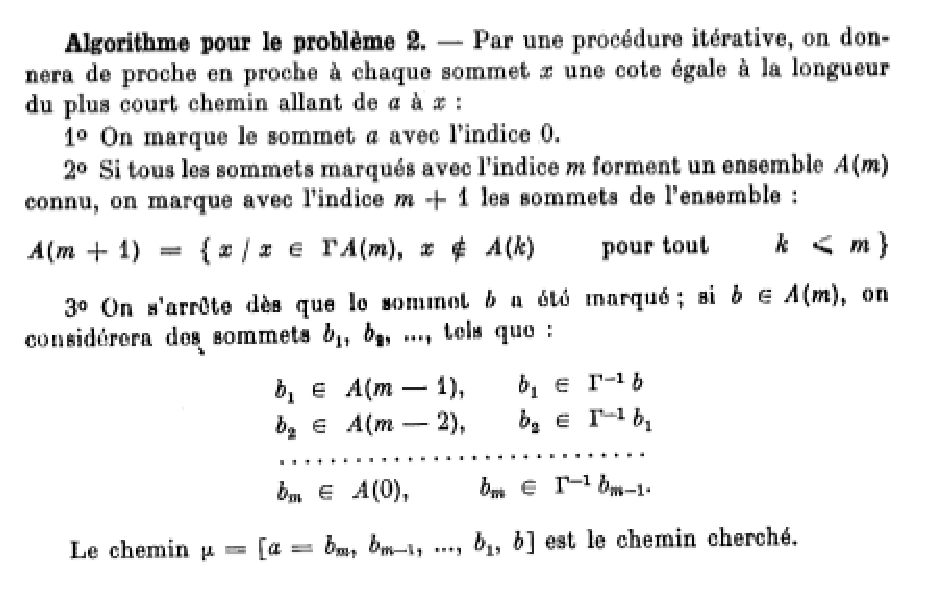
\includegraphics[width=11cm]{berge-alg}
\end{center}
\caption{The original description of the BFS algorithm in
  \cite{bergebook2}.}
\label{f:bergebfs}
\end{figure}

\subsection{Looking for a good route in public transportation}
Consider a bus network with the following timetables:
\begin{center}
\begin{minipage}{2.5cm}
\begin{tabular}{c|c}
\multicolumn{2}{c}{A} \\ \hline
1 & h:00 \\
2 & h:10 \\
3 & h:30
\end{tabular}
\end{minipage}
\begin{minipage}{2.5cm}
\begin{tabular}{c|c}
\multicolumn{2}{c}{B} \\ \hline
1 & h:00 \\
4 & h:20 \\
5 & h:40  
\end{tabular}
\end{minipage}
\begin{minipage}{2.5cm}
\begin{tabular}{c|c}
\multicolumn{2}{c}{C} \\ \hline
2 & h:10 \\
3 & h:20\\
5 & h:30 
\end{tabular}
\end{minipage}  
\begin{minipage}{2.5cm}
\begin{tabular}{c|c}
\multicolumn{2}{c}{D} \\ \hline
4 & h:20 \\
5 & h:40 \\
6 & h:50 
\end{tabular}
\end{minipage}
\begin{minipage}{2.5cm}
\begin{tabular}{c|c}
\multicolumn{2}{c}{E} \\ \hline
2 & h:05 \\
5 & h:10 \\
6 & h:30
\end{tabular}
\end{minipage}
\begin{minipage}{2.5cm}
\begin{tabular}{c|c}
\multicolumn{2}{c}{F} \\ \hline
3 & h:25 \\
4 & h:30 \\
6 & h:40 
\end{tabular}
\end{minipage}
\end{center}
How do we find a convenient itinerary\index{itinerary} from bus stop 1
to bus stop 6, leaving at h:00? 

We model the problem by means of an {\it event
  network}:\index{networj!event} the nodes\index{node!labelled} are
labelled by pairs\index{pair} (bus stop, minutes after the hour), and
an arc\index{arc} $((b_1,m_1),(b_2,m_2))$ denotes: (i) a bus going
from stop $b_1$ at h:$m_1$ to stop $b_2$ at h:$m_2$, if $b_1\not=b_2$;
(ii) waiting at stop $b_1$ from h:$m_1$ to h:$m_2$ if $b_1=b_2$. Each
arc $((b_1,m_1),(b_2,m_2))$ is labelled by the length of time that
separates the events $(b_1,m_1)$ and $(b_2,m_2)$.  For the timetables
above, the event network is given in Fig.~\ref{f:eventgraph}.

\begin{figure}[!ht]
\begin{center}
\includegraphics[width=12cm]{timetable}
\end{center}
\caption{An event network.}
\label{f:eventgraph}
\end{figure}

We apply BFS to the event network of Fig.~\ref{f:eventgraph}, with
$s=(1,00)$. Here is the evolution of the queue $Q$:
\begin{enumerate}
\setlength{\parskip}{-0.2em}
\item $Q=\{(1,00)\}$ (initialization)
\item $Q=\varnothing$ (Step \ref{bfs3})
\item $Q=\{(2,10),(4,20)\}$ (Step \ref{bfs8})
\item $Q=\{(4,20)\}$ (Step \ref{bfs3})
\item $Q=\{(4,20),(3,20),(3,30)\}$ (Step \ref{bfs8})
\item $Q=\{(3,20),(3,30)\}$ (Step \ref{bfs3})
\item $Q=\{(3,20),(3,30),(4,30),(5,40)\}$ (Step \ref{bfs8})
\item $Q=\{(3,30),(4,30),(5,40)\}$ (Step \ref{bfs3})
\item $Q=\{(3,30),(4,30),(5,40),(3,25),(5,30)\}$ (Step \ref{bfs8})
\item $Q=\{(4,30),(5,40),(3,25),(5,30)\}$ (Step \ref{bfs3})
\item $Q=\{(5,40),(3,25),(5,30)\}$ (Step \ref{bfs3})
\item $Q=\{(5,40),(3,25),(5,30),(6,40)\}$ (Step \ref{bfs8}) \\ At this
  point, we know we can get to bus stop 6 at h:40, but since there are
  other nodes labelled with bus stop 6 (one of which has a time label
  h:30), we have to continue and see if there are some other paths
  leading to a better time.
\item $Q=\{(3,25),(5,30),(6,40)\}$ (Step \ref{bfs3}) 
\item $Q=\{(3,25),(5,30),(6,40),(6,50)\}$ (Step \ref{bfs8}) \\
So we can also get to bus stop 6 at h:50.
\item $Q=\{(5,30),(6,40),(6,50)\}$ (Step \ref{bfs3}) 
\item $Q=\{(6,40),(6,50)\}$ (Step \ref{bfs3}) 
\item $Q=\{(6,50)\}$ (Step \ref{bfs3}) 
\item $Q=\varnothing$ (Step \ref{bfs3}). 
\end{enumerate}
Thus we conclude that the most convenient itinerary\index{itinerary}
from stop 1 to stop 6 arrives at 6 at h:40. On the other hand, we
never specified what ``convenient'' really meant. We automatically
assumed it meant ``fast'', but, as we said before, the BFS\index{BFS}
finds shortest paths\index{path!shortest} to all nodes only in terms
of number of edges.\index{edge!number} Since each edge in the event
network\index{network!event} represents a change of mode of
transportation\index{transportation!mode} (there are seven such modes:
waiting, bus A, \dots, bus F), the BFS identifies paths\index{path}
that minimize the number of changes. Since $(6,40)$ is the first
node\index{node} for bus stop 6 that entered the queue,\index{queue}
in view of Cor.~\ref{cor:ultv} the (directed)
path\index{path!directed} $((1,00),(4,20),(4,30),(6,40))$ is the
shortest in terms of number of changes. It suffices to change three
times: bus B from stop 1 to stop 4, then wait for 10 minutes at stop
4, then bus F from stop 4 to stop 6.

\section{Depth-first search}
\label{s:graphalg:dfs}
Let $Q$ be a stack\index{stack} in the {\sc Graph
  Scanning}\index{graph scanning@{\sc Graph Scanning}} algorithm. We
insert and remove elements from one end of the linear data structure
only, using the methods {\tt push()}\index{stack!push} and {\tt
  pop()}.\index{stack!pop} The resulting algorithm is called {\sc
  Depth-First Search}\index{depth-first search@{\sc Depth-First
    Search}} (DFS)\index{DFS}.
\begin{algorithmic}[1]
\REQUIRE $G=(V,E)$, $s\in V$, $R=\{s\}$, $Q=\{s\}$ is a
stack\index{stack}
\WHILE{$Q\not=\varnothing$} \label{dfs1}
  \STATE pop $v$ from the stack $Q$ \label{dfs2} 
  \FOR{$w\in N(v)\smallsetminus R$} \label{dfs5}
    \STATE $R\leftarrow R\cup\{w\}$ \label{dfs7}
    \STATE push $w$ on the stack $Q$ \label{dfs8}
  \ENDFOR
\ENDWHILE
\end{algorithmic}

Understanding DFS may be hard at first. Let us first see the effect on
DFS on a tree.\index{tree}
\begin{eg}
Consider the following tree, setting $s=1$. Boxed elements are on the
stack.
\begin{center}
\begin{minipage}{3.5cm}
\begin{center}
\begin{tikzpicture}
\Tree [.\fbox{1} [.2 3 4 ] [.5 6 ] ]
\end{tikzpicture} \\
{\scriptsize $1$ is pushed}
\end{center}
\end{minipage}
\begin{minipage}{3.5cm}
\begin{center}
\begin{tikzpicture}
\Tree [.1 [.\fbox{2} 3 4 ] [.\fbox{5} 6 ] ]
\end{tikzpicture} \\
{\scriptsize $1$ is popped, $2,5$ are pushed (in this order)}
\end{center}
\end{minipage}
\begin{minipage}{3.5cm}
\begin{center}
\begin{tikzpicture}
\Tree [.1 [.\fbox{2} 3 4 ] [.5 \fbox{6} ] ]
\end{tikzpicture} \\
{\scriptsize $5$ is popped, $6$ is pushed}
\end{center}
\end{minipage}
\begin{minipage}{3.5cm}
\begin{center}
\begin{tikzpicture}
\Tree [.1 [.\fbox{2} 3 4 ] [.5 6 ] ]
\end{tikzpicture} \\
{\scriptsize $6$ is popped}
\end{center}
\end{minipage}
\begin{minipage}{3.5cm}
\begin{center}
\begin{tikzpicture}
\Tree [.1 [.2 \fbox{3} \fbox{4} ] [.5 6 ] ]
\end{tikzpicture} \\
{\scriptsize $2$ is popped, $3,4$ are pushed (in this order)}
\end{center}
\end{minipage}
\begin{minipage}{3.5cm}
\begin{center}
\begin{tikzpicture}
\Tree [.1 [.2 \fbox{3} 4 ] [.5 6 ] ]
\end{tikzpicture} \\
{\scriptsize $4$ is popped}
\end{center}
\end{minipage}
\begin{minipage}{3.5cm}
\begin{center}
\begin{tikzpicture}
\Tree [.1 [.2 3 4 ] [.5 6 ] ]
\end{tikzpicture} \\
{\scriptsize $3$ is popped}
\end{center}
\end{minipage}
\end{center}
So the order of the visit is $1,5,6,2,4,3$. 
\end{eg}

In other words, every path\index{path} from the source\index{source}
to a leaf\index{leaf} is explored by depth\index{depth} first,
backtracking\index{backtrack} from every reached leaf to the closest
ancestor\index{ancestor} (i.e.~previously visited vertex on the same
path) with at least three neighbours,\index{neighbour} or the
source,\index{source} and continuing until each edge\index{edge} has
been traversed exactly twice (once in each direction).  On general
graphs,\index{graph} just imagine the effect of the test $v\not\in R$
at Step \ref{dfs5}: if $v$ was just popped off the stack a node has
already been scanned previously, the edge is ignored.

DFS has been used for several different tasks in graph theory, see
e.g.~the WikiPedia entry \\
\url{http://en.wikipedia.org/wiki/Depth-first_search}.

\subsection{A recursive version of DFS}
DFS can also be written as a recursive
algorithm.\index{algorithm!recursive} This should not be so
surprising, in view of the relationship between stacks\index{stack}
and recursion\index{recursion} discussed in Chapter \ref{c:recursion}.
Given a connected graph\index{graph!connected} $G=(V,E)$ and a source
vertex\index{vertex!source} $s\in V$, consider the following recursive
function\index{function!recursive} {\tt dfs($G,s,R,v$)}:\index{dfs@{\tt dfs}}
\begin{algorithmic}[1]
\FOR{$w\in N(v)\smallsetminus R$} \label{rdfs5}
  \STATE $R\leftarrow R\cup\{w\}$ \label{rdfs7}
  \STATE {\tt dfs($G,s,R,w$)}
\ENDFOR
\end{algorithmic}
The DFS search\index{DFS!search} of $G$ from $s$ is then simply {\tt
  dfs($G,s,\{s\},s$)}.

\begin{ex}
Rewrite the recursive DFS algorithm iteratively by means of a stack,
and verify that it is the same as the DFS algorithm given at the
beginning of Sect.~\ref{s:graphalg:dfs}.
\end{ex}

\subsection{History of the DFS}
The DFS\index{DFS} is one of the oldest methods in graph
theory;\index{graph!theory} its first application was finding the way
out of mazes.\index{maze} Recursion\index{recursion} is easily
explained in this setting: a person {\it inside} a maze can barely be
tele-transported to a different location without actually travelling
through the maze; so that from any visited node, one can only go on
visiting the adjacent nodes, and so on recursively.

U.~Eco,\index{Eco, U.} in {\it The Name of the Rose}, has William of
Baskerville read the following text from an ancient manuscript, which
must have dated before 1300:
\begin{quote}
  {\it To find the way out of a labyrinth, there is only one means.  At
  every new junction, never seen before, the path we have taken will
  be marked with three signs. If, because of previous signs on some of
  the paths of the junction, you see that the junction has already
  been visited, you will make only one mark on the path you have
  taken. If all the apertures have already been marked, then you must
  retrace your steps. But if one or two apertures of the junction are
  still without signs, you will choose any one, making two signs on
  it. Proceeding through an aperture that bears only one sign, you
  will make two more, so that now the aperture bears three. All the
  parts of the labyrinth must have been visited if, arriving at a
  junction, you never take a passage with three signs, unless none of
  the other passages is now without signs.}
\end{quote}
Of course, Eco's book is a novel, not history. Furthermore, the
algorithm looks much more complicated than DFS. Yet there is both
backtracking\index{backtrack} (``retrace your steps'') and the
statement of a theorem about termination. It is also clear that this
algorithm, unlike DFS, allows a searching agent to re-visit some
junctions.\index{junction}

K\"onig, in the chapter of his book \cite{koenig} dedicated to the
labyrinth problem, reports the algorithms of Wiener's, published in
1873, and Tr\'emaux, published in 1882. The latter is now established
\cite{graphhistory} with being the official creator of the
DFS. WikiPedia reports that Tr\'emaux was enrolled at Ecole
Polytechnique (X1876).

R.~Tarjan\index{Tarjan, R.} published a series of works that
established DFS as a very versatile algorithm, which can be used for
many important fundamental tasks in graph theory. For example, DFS can
be used to identify the blocks of a graph\index{graph!block} and the
cut vertices\index{vertex!cut} in linear time. A {\it cut vertex} is a
vertex which, if removed, disconnects the graph. A {\it block} is a
subgraph connected to the rest of the graph by means of a single cut
vertex. 

DFS can also be used to determine whether a graph is
planar\index{graph!planar} (i.e.~whether it can be drawn in the plane
without edge intersections).\index{edge!intersection} On digraphs, DFS
can be used to determine a {\it topological
  order}\index{order!topological} on the vertices of a Directed
Acyclic Graph\index{digraph!acyclic} (DAG).\index{DAG} The vertices of
a DAG are in topological order if they are labelled so that, for any
arc $(u,v)$, we have $u<v$.

\subsection{Easy and difficult natural languages}
In Sect.~\ref{s:tree:language:syntnat}, we explained that
understanding the grammatical structure of
sentences\index{sentence!structure} in natural
languages\index{language!natural} requires them to be parsed into a
derivation tree.\index{tree!derivation} When you hear a sentence,
however, you simply hear a sequence\index{sequence} of
words.\index{word} How is a sequence (a linear structure) turned into
a tree?\index{tree} We may assume that our brain is doing the
parsing,\index{parsing} and that the leaves of the tree are some
fundamental syntactical units to which a basic meaning is
attached. The complex meaning of the whole sentence is then put
together by the brain by combining the basic meanings of the leaves,
retracing each path\index{path} from the leaves to the
root.\index{root}

Under this hypothesis, the brain performs a DFS on the derivation
tree. The memory effort made by the brain is proportional to the tree
depth: one needs to remember all the intermediate vertices along a
path from a leaf to the root in order to build the meaning relative to
that path. The derivation tree of the sentence {\it the soft furry cat
  purrs} (see Fig.~\ref{f:dtree}) has depth 6;
\begin{figure}[!ht]
\begin{center}
\begin{tikzpicture}[scale=1.2]
\node (sentence) at (1,5) {\small\it sentence}; 
\node (names) at (0,4) {\small\it names} edge (sentence); 
\node (verb) at (2,4) {\small{\bf verb} {\it(purrs)}} edge (sentence); 
\node (name) at (0,3) {\small\it name} edge (names); 
\node (article) at (-1,2) {\small{\bf article} {\it (the)}} edge (name); 
\node (adjectives1) at (0.5,2) {\small\it adjectives} edge (name); 
\node (noun) at (2,2) {\small{\bf noun} {\it (cat)}} edge (name); 
\node (adjective1) at (0,1) {\small{\bf adjective}
  {\it (soft)}} edge (adjectives1); 
\node (adjectives2) at (2,1) {\small\it adjectives} edge (adjectives1); 
\node (adjective2) at (2,0) {\small{\bf adjective}
  {\it (furry)}} edge (adjectives2); 
\end{tikzpicture}
\end{center}
\caption{The derivation tree of {\it the soft furry cat purrs}.}
\label{f:dtree}
\end{figure}
the brain must remember at most a sequence of 6
vertices\index{vertex!sequence} to retrace to the root
vertex\index{vertex!root}. Miller, in 1956, proposed that on average,
the human memory can recall seven random words without efforts. In our
setting, we can take this to mean that the maximum ``stack size'' for
the brain is 7. Sentenes are ``simple'' if the depth is 7 or less, and
``complicated'' if more.

The brain, however, also follows a precise order when processing
vertices at Step \ref{dfs5} of the (iterative) DFS algorithm. This
order is that of the temporal arrival of the words to the ear. What is
said before is processed before what is said later. We identify two
``tree shapes'' that are at the extrema of all possible derivation
trees: the {\it regressive trees}, slanted towards the left, and the
{\it progressive trees}, slanted towards the right (see
Fig.~\ref{f:regprogtree}).
\begin{figure}[!ht]
\begin{center}
\begin{tikzpicture}
\Tree [.$\bullet$ [.$\bullet$ [.$\bullet$ [.$\bullet$ $\bullet$ $\bullet$ ]
      $\bullet$ ] $\bullet$ ] $\bullet$ ]
\end{tikzpicture}
\hspace*{1cm}
\begin{tikzpicture}
\Tree [.$\bullet$ $\bullet$ [.$\bullet$ $\bullet$ [.$\bullet$
      $\bullet$ [.$\bullet$ $\bullet$ $\bullet$ ] ] ] ]
\end{tikzpicture}
\end{center}
\caption{Regressive (left) and progressive (right) tree shapes.}
\label{f:regprogtree}
\end{figure}
A regressive derivation tree corresponds to a sentence whose basic
meanings comes later in time: in ``the soft, furry cat purrs'', for
example, the most basic meanings are assigned to the
leaves\index{leaf} {\it cat} and {\it purrs}, the last words to be
heard by the ear. A progressive derivation tree corresponds to a
sentence whose basic meanings come early in time: in ``l'\'eleve
retardataire n'apprend que la moiti\'e des choses qu'on lui
enseigne'', the most basic meanings are assigned to the leaves {\it
  \'eleve}, {\it retardataire} and {\it apprend}, the first words to
be heard.

When DFS is applied to a regressive tree,\index{tree!regressive} it
needs as much stack size\index{stack!size} as the tree
depth.\index{tree!depth} However, when DFS is applied to a progressive
tree,\index{tree!progressive} something different happens: once the
DFS scans\index{DFS!scan} the deepest (and rightmost)
leaf,\index{leaf!rightmost}\index{leaf!deepest} it no longer needs to
backtrack to the root vertex,\index{vertex!root} because the sentence
is finished --- there are no more words being heard! In other words,
your brain makes much less effort with progressive than with
regressive trees. In algorithmic terms, this means that you no longer
need to push vertices on the stack at Step \ref{dfs8} if you process
vertices on a left-to-right order, and you are exploring the rightmost
path \cite{yngve}.

We can draw some linguistic conclusions from all this. Anglosaxon
languages, for example, prefix adjectives to nouns, and are therefore
more regressive: when saying ``soft, furry cat'', your ear hears {\it
  soft} and {\it furry} before {\it cat}, which has the basic meaning:
therefore, the adjectives must be remembered (pushed on the stack)
until the noun occurs. Latin languages decrease this tendency, and are
more progressive: in ``le lion imposant et sauvage'', you do not need
any stack: the basic meaning {\it lion} comes before {\it imposant}
and {\it sauvage}. Somehow, it seems that latin languages are easier
from the brain to handle, as far as the memory effort is
concerned. Classical Latin, on the other hand, is different. Consider
the famous {\it incipit} of the Aeneid's second canto, ``Inde toro
pater {\AE}neas sic orsus ab alto''. Notice how the order looks
random: a literal English translation is ``Thereafter seat father
Eneas thus standing from a high'' (a more successful translation would
be ``Thereafter father Eneas, thus standing from a hight seat''). By
messing up the order of the words in the sentence, it produced
derivation trees requiring a non-temporal order on the $N(v)$ loop in
the DFS Step \ref{dfs5} in order to reconstitute the sentence's
meaning. Perhaps this is why Latin is a dead language.

\section{Finding a spanning tree of minimum cost}
A tree $T=(U,F)$ in a graph $G=(V,E)$ is
spanning\index{tree!spanning}\index{spanning} if $U=V$, as explained
in Sect.~\ref{s:tree:spanning}. Two applications of minimum
cost\index{cost!minimum} spanning trees to networks, whose edges are
assigned costs, were discussed in Sect.~\ref{s:tree:network}. 

\begin{thm}
Let $G=(V,E)$ be a graph and $c:E\to\mathbb{R}$ be an edge cost
function.\index{edge!cost function} Let $T=(R,F)$ be a spanning tree
of $G$. $T$ is of minimum cost if and only if for each proper subset
$U$ of $V$, the unique edge of the cutset\index{cutset}
$\delta(U)$ in $T$ has minimum cost in $\delta(U)$.
\label{thm:sptree}
\end{thm}
\begin{proof}
($\Rightarrow$) Proceed by contradiction, and assume $T$ is of minimum
  cost, but there is a proper subset $U\subsetneq V$ such that the
  unique edge $e$ in $F\cap\delta(U)$ is not of minimum cost. Because
  of the minimal connectedness\index{connectedness!minimal} of $T$,
  removing any edge disconnects $T$ into two trees\index{tree} $T_1$
  and $T_2$, with $T_1$ spanning $U$, and $T_2$ spanning
  $V\smallsetminus U$. By definition of a cutset, every edge in
  $\delta(U)$ has one incident vertex\index{vertex!incident} in $U$
  and the other in $V\smallsetminus U$, so every such edge can be used
  to re-connect $T_1$ and $T_2$ without creating any
  cycles.\index{cycle} Let $f$ be the minimum cost edge in
  $\delta(U)$: then $T'=T_1\cup\{f\}\cup T_2$ is connected, spans all
  $V$, and has no cycles: it is therefore a spanning tree of
  $G$. Moreover, the cost of $T'$ is
  $c(T')=c(T_1)+c(f)+c(T_2)<c(T_1)+c(e)+c(T_2)=c(T)$, so $T$ could not
  be a minimum cost spanning tree, which goes against our assumption.

($\Leftarrow$) Let $T=(R,F)$ be a spanning tree for $G$ such that
  $T\cap\delta(U)=\{e\}$ be an edge of minimum cost in $\delta(U)$ for
  each proper subset $U\subsetneq V$. Let $T'=(U,F')$ be a minimum
  cost spanning tree with $E\cap E'$ as large as possible. Let $f\in
  E\smallsetminus E'$. Because of the minimal connectedness of $T$,
  the removal\index{tree!edge!removal} of $f$ from $T$ disconnects $T$
  into two disconnected trees $T_1,T_2$ spanning respectively a proper
  subset\index{subset!proper} $U\subsetneq V$ and $V\smallsetminus
  U$. Consider the unique edge $g$ in $\delta(U)\cap T'$: if
  $c(g)=c(f)$ then, since $E\cap E'$ is as large as possible, $g=f$;
  but this is impossible since $f$ was chosen to be outside
  $E'$. Also, by the hypothesis on $T$, $f$ must have minimum cost
  within $\delta(U)$. But then $c(g)>c(f)$. So the tree
  $T'[U]\cup\{f\}\cup T'[V\smallsetminus U]$ is different from $T'$
  and has lower cost than $T'$, which is impossible as $T'$ was
  assumed to have minimum cost. Thus $E\smallsetminus E'$ must be
  empty, which implies $E=E'$, which means that $T$ has minimum cost.
\end{proof}

\begin{ex}
Prove that for any proper subset $U\subsetneq V$,
$|F\cap\delta(U)|=1$, and that for any tree $T$ and edge
$e\in\delta(U)$, $T[U]\cup\{e\}\cup T[V\smallsetminus U]$ is a tree.
\end{ex}

Here we give an algorithm to determine a Minimum-cost Spanning
Tree\index{tree!spanning!minimum cost} (MST)\index{MST} based on the
($\Leftarrow$) direction of Thm.~\ref{thm:sptree}. This
algorithm,\index{algorithm!Prim} due to R.~Prim\index{Prim, R.}  and
published in 1957, ``grows'' a spanning tree $T=(R,F)$, initially set
to $(\{s\},\varnothing)$, starting from a source
vertex\index{vertex!source} $s\in V$. At the outset, it selects from
the cutset\index{cutset} $\delta(s)$ the cheapest edge $\{s,w\}$ and
adds it to $F$, also adding $w$ to $R$. The general iteration is as
follows. The cheapest edge\index{edge!cheapest} $\{v,w\}$ is selected
from the cutset $\delta(R)$; by definition, exactly one between $v$
and $w$ is in $R$, assume this to be $v$ without loss of
generality. Then $\{v,w\}$ is added to $F$ and $w$ to $R$.

\subsection{Prim's algorithm: pseudocode}
Here follows a more detailed pseudocode\index{pseudocode} for {{\sc
    Prim's Algorithm}}.\index{prim's algorithm@{\sc Prim's Algorithm}}
Given a weighted graph\index{graph!weighted} $G=(V,E,c)$ where
$c:E\to\mathbb{R}$ is an edge cost function,\index{cost!function} and
a source vertex\index{vertex!source} $s\in V$, it outputs a spanning
tree $T=(R,F)$ of $G$ of minimum cost. We denote the edge weight
$c(\{u,v\})$ by $c_{uv}$ for any edge $\{u,v\}\in E$.  Prim's
algorithm employs the following data structures:\index{data!structure}
\begin{itemize}
\setlength{\parskip}{-0.3em}
\item $R$: set of reached vertices (vertices in the tree)
\item $F$: set of edges in the tree
\item $u$: best next vertex
\item $\zeta:V\smallsetminus R\to\mathbb{R}$: cost of reaching from $R$ a
  vertex outside $R$
\item $\pi:V\smallsetminus R\to R$: immediate predecessor in $T$ to a
  vertex outside $R$.
\end{itemize}
It works by iteratively choosing the best edge $\{u,v\}$ in the
current cutset (containing $u$ but not $v$) and adding $v$ to the
cutset. It terminates when the cutset contains every vertex.
\begin{algorithmic}[1]
\STATE $R=\{s\}$, $F=\varnothing$, $\forall v\in
V$ set $\zeta(v)=\infty$, $\pi(v)=s$ \label{prim1}
\FOR{$w\in N(s)$} \label{prim2}
  \STATE $\zeta(w)=c_{sw}$ \label{prim3}
\ENDFOR
\WHILE{$R\not=V$} \label{prim4}
  \STATE let $u\in V\smallsetminus R$ such that $\zeta(u)$ is
  minimum \label{prim5} 
  \STATE mark $u$ as reached by adding it to $R$ \label{prim6}
  \STATE add the edge $\{\pi(u),u\}$ to $T$ \label{prim7}
  \STATE update $\zeta,\pi$: $\forall v\in N(u)$ \label{prim8}
  s.t.~$\zeta(v)>c_{uv}$, let $\zeta(v)=c_{uv}$ and $\pi(v)=u$.
\ENDWHILE
\end{algorithmic}

\begin{eg}
Here is the effect of Prim's algorithm on the following weighted
graph.
\begin{center}
\begin{tabular}{cccc}
\psfrag{a}{\scriptsize $1$}\psfrag{b}{\scriptsize $2$}
\psfrag{c}{\scriptsize $3$}\psfrag{d}{\scriptsize $4$}
\psfrag{e}{\scriptsize $5$}\psfrag{f}{\scriptsize $6$}
\psfrag{g}{\scriptsize $7$}
\includegraphics[width=4cm]{sptree1} &
\psfrag{a}{\scriptsize $1$}\psfrag{b}{\scriptsize $2$}
\psfrag{c}{\scriptsize $3$}\psfrag{d}{\scriptsize $4$}
\psfrag{e}{\scriptsize $5$}\psfrag{f}{\scriptsize $6$}
\psfrag{g}{\scriptsize $7$}
\includegraphics[width=4cm]{sptree2} &
\psfrag{a}{\scriptsize $1$}\psfrag{b}{\scriptsize $2$}
\psfrag{c}{\scriptsize $3$}\psfrag{d}{\scriptsize $4$}
\psfrag{e}{\scriptsize $5$}\psfrag{f}{\scriptsize $6$}
\psfrag{g}{\scriptsize $7$}
\includegraphics[width=4cm]{sptree3} &
\psfrag{a}{\scriptsize $1$}\psfrag{b}{\scriptsize $2$}
\psfrag{c}{\scriptsize $3$}\psfrag{d}{\scriptsize $4$}
\psfrag{e}{\scriptsize $5$}\psfrag{f}{\scriptsize $6$}
\psfrag{g}{\scriptsize $7$}
\includegraphics[width=4cm]{sptree4} 
\end{tabular}
\\
\begin{tabular}{ccc}
\psfrag{a}{\scriptsize $1$}\psfrag{b}{\scriptsize $2$}
\psfrag{c}{\scriptsize $3$}\psfrag{d}{\scriptsize $4$}
\psfrag{e}{\scriptsize $5$}\psfrag{f}{\scriptsize $6$}
\psfrag{g}{\scriptsize $7$}
\includegraphics[width=4cm]{sptree5} &
\psfrag{a}{\scriptsize $1$}\psfrag{b}{\scriptsize $2$}
\psfrag{c}{\scriptsize $3$}\psfrag{d}{\scriptsize $4$}
\psfrag{e}{\scriptsize $5$}\psfrag{f}{\scriptsize $6$}
\psfrag{g}{\scriptsize $7$}
\includegraphics[width=4cm]{sptree6} &
\psfrag{a}{\scriptsize $1$}\psfrag{b}{\scriptsize $2$}
\psfrag{c}{\scriptsize $3$}\psfrag{d}{\scriptsize $4$}
\psfrag{e}{\scriptsize $5$}\psfrag{f}{\scriptsize $6$}
\psfrag{g}{\scriptsize $7$}
\includegraphics[width=4cm]{sptree7} 
\end{tabular}
\end{center}
\label{eg:prim}
\end{eg}

\begin{ex}
Fill the empty boxes in Example \ref{eg:prim} with the values for
$\zeta,\pi$ at every vertex. 
\end{ex}

\subsection{Complexity of Prim's algorithm}
The initialization takes $O(n)$ (Step \ref{prim2}). The main loop
(Step \ref{prim4}) also takes $O(n)$. The choice of $u$ (Step
\ref{prim5}) takes $O(n)$, the updates of $R,T$ (Steps
\ref{prim6}-\ref{prim7}) take $O(1)$, and the updates of $\zeta,\pi$
(Step \ref{prim8}) takes $O(n)$. Altogether, this is:
\begin{eqnarray*}
O(n + n(n+1+n)) 
&=&  O(n+n^2+n+n^2)  \\ 
&=&  O(2(n + n^2))   \\ 
&=&  O(n+n^2)=O(n^2).
\end{eqnarray*}


%%%%%%%%%%%%%%%%% CHAPTER: PROBLEMS AND COMPLEXITY %%%%%%%%%%%%%%%%%%%%
\chapter{Problems and complexity}
\label{c:problem}

\begin{center}
\fbox{\begin{minipage}{13cm}{\small {\sc Abstract}.  A theoretical
      excursion in the theory of complexity.  Problems and complexity
      classes: {\bf P} and {\bf NP}. {\bf NP}-hard and {\bf
        NP}-complete problems. Exact and heuristic algorithms.  }
\end{minipage}}
\end{center}

\section{Decision problems}
\label{s:problem:decision}
In Sect.~\ref{s:computation:problem} and
\ref{s:recursion:motivation:natural:algprobs}, we defined a problem to
be a set of pairs (input,output).\index{input}\index{output} In fact,
we understand a {\it decision
  problem}\index{problem!decision}\index{decision} to be an
infinite\index{infinite} set of {\it instances},\index{instance} which
are data objects\index{data!object} of the same type,
\index{object!type}\index{data!type} together with a formal question
that can only be answered by YES or NO. For example, the {\sc
  Connected Graph Problem}\index{graph!connected} (CGP) takes as input
an undirected graph $G=(V,E)$ and asks to determine whether the graph
is connected or not. We remark that in order to qualify as a formal
decision problem, the instance set {\it must} be infinite.

In a decision problem, it is not sufficient to guess the answer: we
require a proof. Accordingly, the answer to a given problem
instance\index{problem!instance} must be YES or NO with a {\it
  certificate}\index{certificate} that anyone can check
computationally to establish the truth of the answer. A certificate
may be a combinatorial structure which, by its very presence,
testifies as to the truth of the answer; or a theorem with its formal
proof; or even the printout of all the computation carried out to
obtain the YES or the NO. In the case of the CGP, for example, we
might exhibit a spanning tree\index{tree!spanning} for a YES, or an
empty nontrivial cutset for a NO:\index{cutset!empty!nontrivial} a
graph has a spanning tree if and only if it is connected, and has a
nonempty nontrivial cutset if and only if it is not. Notice that an
instance might have more than one certificate: for the CGP example,
any spanning tree is an acceptable YES certificate, and any nonempty
nontrivial cutset is an acceptable NO certificate.

An infinite subset of instances out of a given problem is sometimes
called a {\it problem case}\index{problem!case} or 
{\it subproblem}.\index{subproblem} For example, the CGP restricted to
cliques\index{clique} is an infinite class of instances (there is a
clique for every integer $n$). Because it is easy to show that every
clique is connected, the answer to each instance of this CGP
subproblem is always YES, and the proof, valid for every instance,
provides an instance-independent certificate.

\section{Optimization problems}
In an {\it optimization problem}\index{problem!optimization} we assign
scalar values\index{value} to all possible YES certificates, and look
for certificates having smallest ({\it
  minimization})\index{minimization} or greatest ({\it
  maximization})\index{maximization} value. If an instance of an
optimization problem is a NO instance, we simply require the proof for
the NO (no scalar values are assigned to NO instances).

The {\sc Minimum Spanning Tree}\index{minimum spanning tree@{\sc
    Minimum Spanning Tree}} (MST)\index{MST}
problem\index{problem!MST} is an example of an optimization
problem. Disconnected graph\index{graph!disconnected} instances are NO
instances,\index{instance!NO} whilst all connected weighted graphs
provide YES instances,\index{instance!YES} and among the set of all
spanning trees we require one with minimum cost\index{cost!minimum}
(more than one spanning tree might have minimum cost: consider the
case where all edges have unit weight).

\subsection{Relationship between decision and optimization}
\label{s:problem:decopt}
The abstract decision problem\index{problem!decision!abstract} is as
follows. Given a set $U$ and a subset\index{subset} $V$ of $U$,
determine whether $V$ is empty\index{empty} or not. The abstract
optimization problem\index{problem!optimization!abstract} would add a
scalar-valued function\index{function!scalar-valued}
$\mu:U\to\mathbb{R}$ and ask to determine whether $V$ is empty, and,
if not, find $v\in V$ with maximum or minimum $\mu$
value.\index{value!maximum}\index{value!minimum}

Let $M=\{\mu(u)\;|\;u\in U\}$. A minimization
problem\index{problem!minimization} $(U,V,\mu)$ on a finite set $U$
can be solved by solving $O(\log|M|)$ decision
problems\index{problem!decision} $(U,V_\alpha)$ defined by
$V_\alpha=\{v\in V \;|\;\mu(v)\le\alpha\}$. We proceed by
bisection\index{bisection} (see Sect.~\ref{s:sort:bisection}) on the
scalar set\index{set!scalar} $M$. We start with $\alpha$ set to the
median\index{median} of $M$, and solve $(U,V_\alpha)$. If
$V_\alpha=\varnothing$ we replace $M$ by $\{\beta\in
M\;|\;\beta>\alpha\}$, otherwise by $\{\beta\in
M\;|\;\beta\le\alpha\}$, and we repeat. By the familiar
bisection\index{bisection} argument,\footnote{See INF311.}  we need at
most $O(\log|M|)$ iterations before a $v\in V$ minimizing $\mu$ is
found.

\begin{ex}
Adapt the above algorithm to the maximization case.
\end{ex}

\begin{ex}
Why does $U$ need to be finite, in the above algorithm?
\end{ex}

For example, the MST\index{MST} problem is equivalent to solving a set
of decision problems of the form, ``given a weighted graph, and a
scalar $k$, does it have a spanning tree with cost less than $k$?''.

\section{Algorithms}
In this context, we require an algorithm\index{algorithm} to solve a
problem, rather than a finite set of instances. Procedures that only
work with a certain graph,\index{graph} or a finite set of graphs are
not considered algorithms. Instead, an algorithm is the description of
a computational procedure, which takes {\it any}
instance\index{instance} as an input,\index{input} and provides an
answer with its proof (it might even fail to
terminate\index{termination!failure} if the problem is
undecidable).\index{problem!undecidable}

\section{Complexity}
\label{s:problem:complexity}
The interest in grouping infinite sets of instances into problems, and
to only consider algorithms that can potentially solve all instances
of a problem, is to provide asymptotic answers with respect to
algorithmic complexity. We are mainly interested in three points of
view. First, what is the complexity of an algorithm for a given
problem? This is discussed in
Sect.~\ref{s:computation:complexity}-\ref{s:computation:complexityorder},
and, via worst-case complexity\index{complexity!worst-case}, aims to
establish an upper bound\index{complexity!upper bound} for the
asymptotic complexity of an algorithm as the instance size increases.

Secondly: what is the algorithm that performs most efficiently on a
given problem?  This point of view goes under the name of {\it problem
  complexity},\index{problem!complexity}\index{complexity!problem} and
aims to establish a lower bound\index{complexity!lower bound} for the
asymptotic worst-case complexity of the best algorithm for solving the
problem as the instance size increases.

Typically, in the first case, we want to establish results like ``the
complexity\index{complexity!algorithm} of Prim's
algorithm\index{algorithm!Prim's} is $O(n^2)$.''  In the second case,
we want to establish results like ``the MST
problem\index{problem!MST!complexity} has polynomial
complexity\index{complexity!problem}''. Notice that, in the second
case, there might be other algorithms that take an exponential time to
solve the MST in the worst-case (such as for example listing all
spanning trees), but we only focus on the best. The second case is an
abstraction\index{abstraction} of the first: whereas we looked at
single algorithms in the first case, we look at the best over {\it
  all} algorithms for a given problem in the second case.

We look at the third point of view in Sect.~\ref{s:problem:class}.

\section{Easy and difficult problems}
\label{s:problem:class}
The third point of view abstracts problems too. We group problems into
{\it problem classes}\index{problem!class} and classify them by
algorithmic efficiency:\index{efficiency!algorithmic} we have a
problem class {\bf P}\index{P@{\bf P}} of all decision problems that can
be solved in worst-case asymptotic time bounded by a
polynomial\index{polynomial} in the instance
size,\index{instance!size} and a problem class {\bf NP}\index{NP@{\bf
    NP}} of all decision problems whose YES
certificates\index{certificate!YES} can be verified in worst-case
asymptotic time bounded by a polynomial in the instance size (notice
we do not require any condition on NO
certificates),\index{certificate!NO} as well as many other problem
classes. Informally, {\bf P} is the class of problems that are
``easy'' to solve, whereas {\bf NP} is the class of problems whose
solutions can be verified efficiently. 

So we have a formal way to say a problem is easy (it can be solved in
polynomial time), and a formal way to say the solutions of a problem
are easy to check. How about a formal way to say that a problem is
difficult? In \cite{gareyjohnson}, Garey and Johnson\index{Garey,
  M.}\index{Johnson, D.} argue that a convenient way to do so would be
to say that a problem is difficult if no-one could solve it
efficiently to date. The formalization of this concept is {\bf
  NP}-hardness.

\subsection{Reductions}
\label{s:problem:reduction}
Suppose we are given a new problem $P$ for which we have to conceive
and implement a solution algorithm.\index{algorithm} We might notice
and exploit a certain similarity between $P$ and a problem we already
know how to solve, say $Q$. For example, suppose $P$ is the problem of
finding a stable\index{stable} (see
Sect.~\ref{s:graph:subgraph:stable}) with at least $k$ vertices in a
graph $G$, for given $k$ and $G$ (this problem is known as {\sc
  $k$-Stable}\index{$k$-stable@{\sc $k$-Stable}}). The similarity is
usually derived theoretically; consider for example the following
result.
\begin{lem}
Given a graph $G=(V,E)$ and $U\subseteq V$, $U$ is a stable
set\index{stable!set} of $G$ if and only if $\bar{G}[U]$ is a
clique\index{clique} in $\bar{G}$.
\label{lem:cliqstab}
\end{lem}
\begin{proof}
($\Rightarrow$) Since $U$ is a stable in $G$, the edge
  set\index{edge!set} of $G[U]$ is empty by definition. Thus, in the
  complement graph,\index{graph!complement} the edge set of
  $\bar{G}[U]$ is complete,\index{complete} i.e.~$\bar{G}[U]$ is a
  clique in $G$. The ($\Leftarrow$) direction is symmetric.
\end{proof}

According to Lemma \ref{lem:cliqstab}, we can take $Q$ to be the
problem of finding a clique\index{clique} in $G$ with at least $k$
vertices (this problem is known as {\sc
  $k$-Clique}\index{$k$-clique@{\sc $k$-Clique}}). Now an algorithm
for solving $P$, given a graph $G$ and the integer\index{integer} $k$,
is as follows:
\begin{enumerate}
\item construct the complement graph\index{graph!complement} $\bar{G}$
\item solve $Q$ on $\bar{G}$ to obtain a clique\index{clique}
  $C=(U,F)$ in $\bar{G}$ 
\item return $U$ as a stable set\index{set!stable} with $k$
  vertices\index{vertex} in $G$ 
\end{enumerate}
Notice the structure of this algorithm: first we transform the
input\index{input} of $P$ to the input of $Q$, then we solve $Q$, then
we transform the output\index{output} of $Q$ back to the output of
$P$. In our example, by Exercise \ref{ex:complement} the complement
graph can be constructed in polynomial time.\index{polynomial time} If
both input and output transformations can be carried out in polynomial
time, we obtain a {\it polynomial
  reduction}\index{reduction!polynomial} of $P$ to $Q$.

\subsection{The new problem is easy}
If we were able to carry out both transformations in polynomial time
and $Q$ were in {\bf P}, we would have found a polynomial algorithm
for $P$ (transform the given $P$ instance into a $Q$ instance in
polynomial time, solve the $Q$ instance in polynomial time, then
transform the solution of the $Q$ instance back into a solution of the
$P$ instance in polynomial time), and we would have thus shown that
$P\in\mbox{\bf P}$ too.

We remark that, so far, no-one was able to show that the problem of
finding a $k$-clique subgraph\index{subgraph!$k$-clique} of $G$ is in
{\bf P}. So our example with cliques and stables does not fall in this
category.

\subsection{The new problem is as hard as another problem}
If we intuitively believe that $P$ is a difficult problem, as seems to
be the case with {\sc $k$-Stable}, it makes little sense to try and
reduce it to an easy one. As mentioned above, one way to show $P$ is
difficult is to show that every other ``intuitively difficult''
problem polynomially reduces to $P$. In other words, if $P$ could be
solved efficiently, every ``intuitively difficult'' problem could also
be solved efficiently by transforming an instance to an instance of
$P$, then solve $P$, then transform the output back to the difficult
problem (notice this exchanges the roles of $P$ and $Q$ in
Sect.~\ref{s:problem:reduction}). In this setting, $P$ being easy
seems unlikely, for it would mean that everyone had a wrong intuition
about the difficulty of all other ``intuitively difficult'' problems.

\subsection{{\bf NP}-hardness and {\bf NP}-completeness}
In order to formalize the discussion in the previous section, we
define the problem $P$ to be {\bf NP}-{\it hard}\index{NP-hard@{\bf
    NP}-hard} if every problem in {\bf NP} can be polynomially reduced
to $P$. We define $P$ to be {\bf NP}-{\it
  complete}\index{NP-complete@{\bf NP}-complete} if it is {\bf
  NP}-hard and also belongs to {\bf NP}.

\begin{eg}
\label{eg:nphard}
It turns out that {\sc $k$-Clique}\index{$k$-clique@{\sc $k$-Clique}}
is {\bf NP}-complete. The problem {\sc Max Clique}\index{max
  clique@{\sc Max Clique}}, which asks to find the greatest complete
subgraph\index{subgraph!complete} in a given graph, is {\bf NP}-hard:
since it is an optimization problem, and {\bf NP} is a subclass of all
decision problems, by definition {\sc Max Clique} cannot belong to
{\bf NP}.\index{NP@{\bf NP}} We emphasize, however, that {\sc $k$-Clique}
is the ``decision version'' of the {\sc Max Clique} optimization
problem, in the sense given in Sect.~\ref{s:problem:decopt}.
\end{eg}

This leaves us with just one basic question: how can we possibly hope
to reduce {\it every problem} in {\bf NP} to a specific problem $P$?
S.~Cook\index{Cook, S.} first provided a proof of {\bf
  NP}-completeness: he encoded a Turing Machine\index{Turing!Machine}
with certain properties into a propositional
formula.\index{formula!propositional} With Cook's approach, ``every
problem in {\bf NP}'' was replaced by the TM\index{TM} used for its
solution. Once a single problem is shown to be {\bf NP}-hard, it can
also be used as a representative of ``every problem in {\bf
  NP}''. Cook's theorem thus paved the way for decades of polynomial
reduction based {\bf NP}-hardness proofs.

Back to our stables and cliques, since by Example \ref{eg:nphard} we
know that {\sc $k$-Clique}\index{$k$-clique@{\sc $k$-Clique}} is {\bf
  NP}-complete, reducing it to {\sc $k$-Stable}\index{$k$-stable@{\sc
    $k$-Stable}} proves that the latter is also {\bf NP}-complete. But
this is easily done, since Lemma \ref{lem:cliqstab} is an ``if and
only if'' result, and the polynomial reduction works both ways. So we
conclude that {\sc $k$-Stable} is at least as hard to solve as the
most difficult problems in {\bf NP}. 

\subsection{The most celebrated conjecture in computer science}
It would be very nice if we were able to turn the definition of a
difficult problem from ``no-one else can solve it efficiently'' to
``it is impossible to solve it efficiently''. Translated in the formal
terminology about {\bf P} and {\bf NP}, the latter corresponds to
proving that $\mbox{\bf P}\not=\mbox{\bf NP}$, i.e.~there is at least
one problem in {\bf NP} that cannot be solved in polynomial time {\it
  for sure}. $\mbox{\bf P}\not=\mbox{\bf NP}$ is the most celebrated
conjecture in computer science. The first person who is able to
establish whether $\mbox{\bf P}\not=\mbox{\bf NP}$ or $\mbox{\bf
  P}=\mbox{\bf NP}$ stands to gain hefty monetary rewards, too.
Unfortunately, four decades of work in this sense yielded no
definitive result yet. Since we value our intuition, and we would not
like to think that someone in the future will be able to show that all
the problems we thought difficult are really easy, people say it is
unlikely that $\mbox{\bf P}=\mbox{\bf NP}$. The method for proving
$\mbox{\bf P}=\mbox{\bf NP}$ would seem straightforward: simply find a
polynomial algorithm\index{algorithm!polynomial} for any {\bf NP}-hard
problem.\index{problem!NP-hard@{\bf NP}-hard} On the other hand, no
convincing proof methodology for even attempting to prove the converse
was found to date.

J.~Edmonds,\index{Edmonds, J.} who first proposed that efficient
algorithms are those that run in time bounded by a polynomial in the
instance size, once said during a seminar at the Institut Poincar\'e
in Paris, that G\"odel's incompleteness theorem (see
Sect.~\ref{s:recursion:goedel}) is at play here, and that $\mbox{\bf
  P}\not=\mbox{\bf NP}$ is true but cannot be proved from the standard
axioms.

\subsection{The student's pitfall}
When asked to show the {\bf NP}-hardness\index{NP-hard@{\bf NP}-hard}
of problem $P$, every student seems to step in the following pitfall:
he or she reduces $P$ to another {\bf NP}-hard problem $Q$, then
claims the work is done. This is wrong! Remember:
\begin{enumerate}
\item If $Q$ is in {\bf P}, then a polynomial reduction $P\to Q$ proves $P$ is
  also in {\bf P}.
\item If $Q$ is {\bf NP}-hard, then a polynomial reduction $Q\to P$
  proves $P$ is also {\bf NP}-hard.
\end{enumerate}
By contrast, polynomially reducing $Q$ to $P$ when $Q$ is in {\bf P},
or $P$ to $Q$ when $Q$ is {\bf NP}-hard proves absolutely nothing.

\section{Exact and heuristic algorithms}
\label{s:problem:exactheur}
So what do we do after we decide whether a new problem $P$ is easy or
difficult? In the first case, the polynomial reduction automatically
gives an exact algorithm\index{algorithm!exact} for finding guaranteed
solutions, as we saw in Sect.~\ref{s:problem:reduction}.  We might
perhaps wish to improve or fine-tune that algorithm, but essentially
we are able to find exact solutions of $P$.

If $P$ turns out to be difficult, we can either use a
non-polynomial\index{algorithm!non-polynomial} solution algorithm to
find exact and guaranteed solutions, or use {\it heuristic
  algorithms}:\index{algorithm!heuristic}\index{heuristic} these are
methods based on intuitive common sense, which do their best to try
and find solutions in a limited amount of time (or
resources).\index{time!limited}\index{resource!limited} If they do,
these solutions are valid; but if they do not, this does not imply
that the input instance is NO. 

Heuristic algorithms for optimization
problems\index{problem!optimization} provide solutions which may not
be optimal,\index{solution!optimal} but are supposed to be ``good
enough''.

\subsection{A heuristic method for {\sc Max Stable}}
Since {\sc Max Stable}\index{max stable@{\sc Max Stable}} is {\bf
  NP}-hard,\index{NP-hard@{\bf NP}-hard} and it seems unlikely that
{\bf P}$=${\bf NP}, we provide a greedy\index{greedy}
heuristic\index{heuristic!greedy} for solving this problem. Our
heuristic is based on the idea that any maximum
stable\index{stable!maximum} is also maximal.\index{stable!maximal} We
recall that a stable is maximum if it has largest
cardinality\index{cardinality!largest} among all stable sets of the
graph; and a stable is maximal if there is no larger stable containing
it as a subset. In other words, the ``maximum'' property needs to be
checked globally (which is time-consuming), whereas the ``maximal''
property only needs to be checked locally (which is much more
efficient).

\begin{ex}
Prove formally that any maximum stable is also maximal. Show that the
converse is not necessarily true.
\end{ex}

Although maximal stables are not necessarily maximum, they might be:
after all, maximality is a necessary, if not sufficient, condition to
be maximum. Moreover, maximal sets can be ``grown'' efficiently by
simply adding all elements until it is possible to do so. We start
from an empty stable $U$, then scan all vertices of $V$, adding them
to $U$ as long as no pair of vertices in $U$ is adjacent to an
edge. We can actually improve on this algorithm by ordering the
vertices first.
\begin{algorithmic}[1]
\STATE $U=\varnothing$;
\STATE order $V$ by increasing values of $|N(v)|$;
\WHILE{$V\not=\varnothing$}
   \STATE $v=\min V$;
   \STATE $U\leftarrow U\cup \{v\}$;
   \STATE $V\leftarrow V\smallsetminus (\{v\}\cup N(v))$ \label{maxstab}
\ENDWHILE
\end{algorithmic}

\begin{ex}
Explain the presence of Step \ref{maxstab}: does it improve the
algorithm? If so, why? If not, why not?
\end{ex}

%%%%%%%%%%%%%%%%% CHAPTER: SORTING %%%%%%%%%%%%%%%%%%%%
\chapter{Sorting}
\label{c:sort}

\begin{center}
\fbox{\begin{minipage}{13cm}{\small {\sc Abstract}.  
The searching problem and the sorting problem: complexity in the best
case. Sorting algorithms: selection, insertion, merge and quick
sort. Two-way partitioning.
}
\end{minipage}}
\end{center}


Let $V=(v_1,\ldots,v_n)$ be a sequence\index{sequence} with a natural
order\index{order!natural} $<$ defined on its elements. The sequence
$V$ is {\it sorted}\index{sequence!sorted}\index{sorted} if:
\begin{equation}
  \forall i<j\le n\quad v_i\le v_j, 
  \label{eq:sort}
\end{equation}
and {\it unsorted}\index{sequence!unsorted}\index{unsorted} otherwise.

\section{The searching problem}
\label{s:sort:searching}
A fundamental question that often occurs in algorithms is whether a
given set $V$ contains a given element $u$. This is a decision
problem\index{problem!decision} with input\index{input} $V,u$, called
the {\sc Searching Problem}\index{searching problem@{\sc Searching
    Problem}}. If $V$ is unsorted,\index{unsorted}
searching\index{searching} takes longer than if $V$ is
sorted,\index{sorted} as shown below. In this chapter we discuss
methods for sorting linear data
structures.\index{data!structure!linear}

\section{Searching unsorted and sorted arrays}
\label{s:sort:bisection}
If $V=(v_1,\ldots,v_n)$ is stored as a linear data
structure,\index{data!structure!linear} say an array,\index{array} and
this array is unsorted,\index{array!unsorted}\index{unsorted} the only
possible approach is brute force:\index{brute force} verify each
element of $V$ in turn, and stop with YES when $v$ is found, or
terminate with NO at the end of the array. This method is obviously
$O(n)$.

If the array were sorted,\index{array!sorted}\index{sorted} on the
other hand, we could proceed using bisection.\index{bisection} Here is
the recursive pseudocode\index{pseudocode!recursive} for {\tt
  bisection($V,w$)}.\index{bisection}
\begin{algorithmic}[1]
\REQUIRE $V=\{v_1,\ldots,v_n\}$ is sorted
\IF{$V=\varnothing$}
  \RETURN NO
\ENDIF
\STATE let $i=\lceil\frac{n}{2}\rceil$
\IF{$u=v_i$}
  \RETURN YES
\ELSIF{$u<v_i$}
  \STATE let $V=\{v_{1},\ldots,v_{i-1}\}$
\ELSIF{$u>v_i$}
  \STATE let $V=\{v_{i+1},\ldots,v_n\}$
\ENDIF
\RETURN {\tt bisection($V,u$)}
\end{algorithmic}
It is well known\footnote{See INF311.} that the worst-case complexity
of {\tt bisection} is $O(\log n)$.

So, if an algorithm needs to repeatedly test for membership in $V$, it
makes sense to invest some CPU time to sort $V$ first, prior to
calling the membership test procedure.

\section{The sorting problem}
The {\sc Sorting Problem}\index{sorting problem@{\sc Sorting Problem}}
(SP)\index{SP} is as follows. Given a sequence\index{sequence}
$s=(s_1,\ldots,s_n)$ of elements of a set $S$ endowed with a total
order\index{order!total} $<$, find a permutation\index{permutation}
(see Sect.~\ref{s:recursion:permutation}) $\pi$ of $n$ symbols such
that $\pi s=(s_{\pi(1)},\ldots,s_{\pi(n)})$ satisfies
Eq.~\eqref{eq:sort}. In other words, we want to order $s$ according to
$<$.

\subsection{Considerations on the complexity of SP}
In Sect.~\ref{s:problem:complexity}, we discussed two types of
complexity: the complexity\index{complexity!algorithm} of an algorithm
(how long it takes to execute), and the complexity of a
problem,\index{complexity!problem} i.e.~how long does the {\it best}
algorithm\index{algorithm!best} for the problem takes to execute. In
Sect.~\ref{s:problem:class} we went on to classify problems according
to whether they are known or unknown to have polynomial
complexity.\index{complexity!polynomial} 

\subsubsection{The best algorithm for a problem}
In fact, however, we do not need to know the best possible algorithm
that solves a given problem to state that the problem belongs to the
class {\bf P}: it suffices for this purpose to find at least {\it one}
polynomial algorithm,\index{algorithm!polynomial} even if it is not
the best possible. This is rather lucky, because proving that a
certain algorithm is best for a given problem seems to require looking
at the infinite class\index{class!infinite} of all algorithms solving
the problem. This task is so difficult that, if one could prove that
the best algorithm\index{algorithm!exponential} for solving an {\bf
  NP}-complete problem\index{problem!NP-complete@{\bf NP}-complete}
(such as e.g.~{\sc $k$-Stable})\index{$k$-stable@{\sc $k$-Stable}} is
exponential, one would have settled the $\mbox{\bf P}\not=\mbox{\bf
  NP}$ conjecture.\index{conjecture}

\subsubsection{The $\Omega(\cdot)$ and $\Theta(\cdot)$ notations}
We introduced in Sect.~\ref{s:computation:complexityorder} the
$O()$\index{$O(\cdot)$} notation to express asymptotic worst-case
complexity:\index{complexity!worst-case}\index{complexity!asymptotic}
a function $t(n)$ is $O(p(n))$ if there is an $N\in\mathbb{N}$ such
that, for all $n>N$, $t(n)\le p(n)$. There is also a notation for the
asymptotic {\it best-case complexity}:\index{complexity!best-case} a
function $t(n)$ is $\Omega(p(n))$\index{$\Omega(\cdot)$} if there is
an $N\in\mathbb{N}$ such that, for all $n>N$, $t(n)\ge p(n)$ ---
incidentally, if a function $t(n)$ is both $O(n)$ and $\Omega(n)$, we
say it is $\Theta(n)$.\index{$\Theta(\cdot)$} Best-case complexity is
the correct notation for the difficult task we mentioned above: can we
say that SP\index{SP} is $\Omega(p(n))$ for some function $p$?

\subsection{Best-case complexity of SP}
SP is one of those few cases where we can say something about the
best-case complexity of a problem. We must, however, assume no prior
knowledge of the type of data\index{data!type} stored in $S$.

More precisely, we assume that the only way to conclude that $u<v$ in
$O(1)$ is to call the machine language\index{language!machine}
instruction for comparing bytes\index{byte!comparison} a
constant\index{constant} number of times. This may not always be the
case: for example, if we knew a priori that $S=\{0,1\}$, we could
conclude that $u<v$ in $O(1)$ by testing whether $u\not=v$ and
$u=0$. 

Any sorting algorithm capable of dealing with any input
set\index{set!input} $S$ must be a set of instructions
(tests,\index{test} loops,\index{loop} etc.)  containing a
sufficiently large number of {\it comparisons}:\index{comparison}
these are tests establishing whether $u<v$ or not. Informally, our
requirement aims at generality: if our algorithm must be able to cater
for all data types, then it must make use of comparisons. This endows
SP with sufficient structure to make us able to reason on its
best-case complexity.

\subsubsection{The sorting tree}
Accordingly, we can describe any comparison-based sorting algorithm
via a {\it sorting tree},\index{tree!sorting} which represents the
logical flow of the sorting algorithm based on the comparisons only.

\begin{eg}
Here is a sorting tree for sorting $s=(s_1,s_2,s_3)$.
\begin{center}
\psfrag{12}{$s_1\overset{?}{\leq}s_2$}
\psfrag{13}{$s_1\overset{?}{\leq}s_3$}
\psfrag{23}{$s_2\overset{?}{\leq}s_3$}
\psfrag{123}{$e$}
\psfrag{132}{$(23)$}
\psfrag{312}{$(132)$}
\psfrag{213}{$(12)$}
\psfrag{231}{$(123)$}
\psfrag{321}{$(13)$}
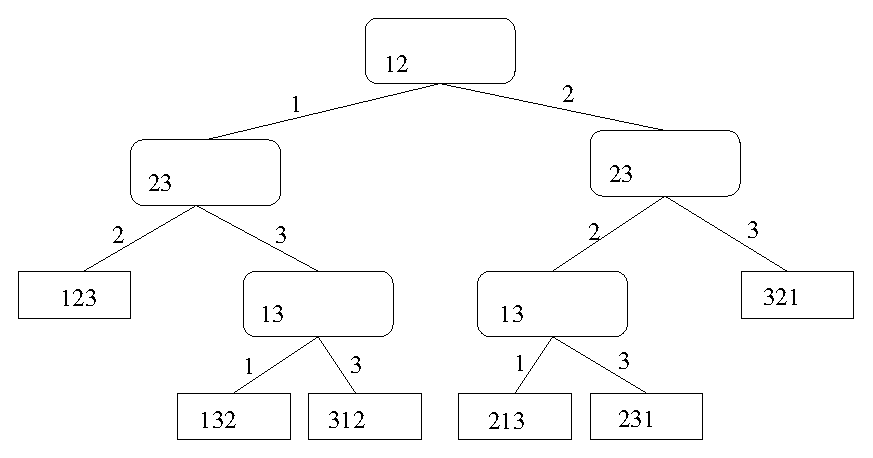
\includegraphics[width=10cm]{dectree}
\end{center}
In the picture above, $e$ stands for the identity
permutation;\index{permutation!identity} the other permutations are
expressed in cycle notation\index{permutation!cycle} (see
Sect.~\ref{s:recursion:permutation:cycle}).
\end{eg}

Sorting trees represent the possible ways to chain comparisons as to
sort all possible input sequences of a given size; moreover, as
mentioned earlier, any comparison-based sorting
algorithm\index{algorithm!sorting!comparison-based} running over input
of given size corresponds to a particular sorting
tree.\index{tree!sorting}\index{sorting!tree} In other words, the set
of all execution traces out of any possible comparison-based sorting
algorithm is a subset of all sorting trees. Hence, the best-case
complexity can be defined in terms of the best sorting trees.

\subsubsection{Formalizing the idea}
\label{s:sorting:complexity:best}
Let $\mathbb{T}_n$ be the set of all sorting trees for
sequences\index{sequence} of length $n$. Different inputs lead to
different permutations in the leaf nodes\index{node!leaf} of each
sorting tree.\index{tree!sorting} For a sorting tree
$T\in\mathbb{T}_n$ and a permutation $\pi$, we denote by $\ell(T,\pi)$
the length of the path\index{path} in $T$ from the root\index{root} to
the leaf\index{leaf} containing $\pi$.
For each $n\ge 0$ we can express the best-case complexity for SP
as:
\begin{equation*}
  B_n = \min_{T\in\mathbb{T}_n} \max_{\pi\in S_n} \ell(T,\pi).
\end{equation*}

We remark that sorting trees are binary trees\index{tree!binary},
since there are only two answers (YES or NO) to each
comparison.\index{comparison} Notice that a binary tree with
depth\index{tree!depth} bounded by $k$ has at most $2^k$
nodes.\index{node} Let $T^\ast$ be the sorting tree of the best
sorting algorithm:\index{algorithm!sorting!best} its number $t$ of
nodes must then be at most $2^{B_n}$. Moreover, since any sorting
tree\index{tree!sorting} lists all $n!$ possible
permutations\index{permutation} in its leaves, it must have at least
$n!$ nodes. Hence $n!\le t\le 2^{B_n}$, whence $n!\le 2^{B_n}$, which
implies
\begin{equation*}
  B_n\ge \lceil \log n!\rceil.
\end{equation*}
By Stirling's\index{Stirling} approximation\index{approximation}
formula\index{formula!Stirling} \cite{cameron2}, $\log n!=n\log
n-\frac{1}{\ln 2}n+O(\log n)$, so we can conclude that $B_n$ is
bounded below by a function proportional to $n\log n$, i.e.~$B_n$ is
$\Omega(n\log n)$.

\section{Sorting algorithms}
There are scores of general-purpose
algorithms\index{algorithm!sorting!general-purpose} for sorting a
sequence\index{sequence} $s=(s_1,\ldots,s_n)$ of elements from a
totally ordered set\index{set!totally ordered} $S$. Many work well
with some sequences but not with others. Here we only discuss a couple
of the simplest algorithms (selection\index{sort!selection} and
insertion sort),\index{sort!insertion} together with two of the best
(merge\index{sort!merge} and quick sort).\index{sort!quick}

\subsection{Selection sort}
In {\sc Selection Sort}\index{selection sort@{\sc Selection
    Sort}}\index{sort!selection} we start from $s=(s_1,\ldots,s_n)$
and end with a sorted sequence $t$, initially empty. We iteratively
select the minimum element\index{element!minimum} of $s$, move it to
the leftmost\index{slot!free!leftmost} free slot in $t$, and remove it
from $s$. Since selecting the minimum from an unsorted
array\index{array!unsorted} requires scanning the whole
array,\index{array!scanning} this takes $O(n^2)$ in the worst case.

\begin{eg}
Let $s=(3,1,4,2)$ and $t=\varnothing$. {\sc Selection Sort} performs the
following sequence of steps:
\begin{eqnarray*}
(3,\fbox{$1$},4,2),\varnothing &\to& (3,4,\fbox{$2$}),(1) \\
                               &\to& (\fbox{$3$},4),(1,2) \\
                               &\to& (\fbox{$4$}),(1,2,3) \\
                               &\to& \varnothing,(1,2,3,4).
\end{eqnarray*}
\end{eg}

\subsection{Insertion sort}
{\sc Insertion Sort}\index{insertion sort@{\sc Insertion
    Sort}}\index{sort!insertion} is somehow dual to {\sc Selection
  Sort}: instead of choosing the minimum\index{minimum} from $s$, we
iteratively choose the leftmost element\index{element!leftmost} of
$s$, insert it in $t$ at the correct position,\index{position!correct}
and remove it from $s$. Since finding the correct position in $t$
requires scanning $t$, this takes $O(n^2)$ in the worst
case. Empirically, {\sc Insertion Sort} is known to be fast for small
values of $n$.

\begin{eg}
Let $s=(3,1,4,2)$ and $t=\varnothing$. {\sc Insertion Sort} performs
the following sequence of steps: 
\begin{eqnarray*}
(\fbox{$3$},1,4,2),\varnothing &\to& (\fbox{$1$},4,2),(3) \\
     &\to& (\fbox{$4$},2),(1,3) \\
     &\to& (\fbox{$2$}),(1,3,4) \\
     &\to& (1,2,3,4).
\end{eqnarray*}
\end{eg}

\begin{ex}
Implement {\sc Insertion Sort} in Java. What data structure did you
employ for $t$?
\end{ex}

\subsection{Merge sort}
{\sc MergeSort}\index{mergesort@{\sc
    MergeSort}}\index{sort!merge}\index{merge} is a recursive
algorithm\index{algorithm!recursive} of the {\sc
  Divide-and-Conquer}\index{divide-and-conquer@{\sc
    Divide-and-Conquer}} class.

\subsubsection{Divide and conquer}
\label{s:sort:merge:divconq}
{\sc Divide-and-Conquer}\index{divide-and-conquer@{\sc
    Divide-and-Conquer}} names a family of algorithms that split a
complex problem\index{problem!complex} into two or more
subproblems\index{subproblem} having the same structure, recursively
solve each of them (the recursion\index{recursion} is on the problem
size),\index{problem!size} then recombine the partial
solutions\index{solution!partial} from both
subproblems\index{subproblem} to construct a solution\index{solution}
of the original problem. {\sc Divide-and-Conquer} is essentially
recursion\index{recursion} (see Chapter \ref{c:recursion}) combined
with bisection\index{bisection} (see Sect.~\ref{s:problem:decopt} and
\ref{s:sort:bisection}).

\subsubsection{Pseudocode}
The idea of {\sc MergeSort}\index{mergesort@{\sc MergeSort}} is to
partition $s$ mid-way and create two smaller unsorted subsequences
$s',s''$, sort each of them recursively, and recombine the sorted
subsequences so that the sorting of the resulting sequence is
maintained. Here is {\tt mergeSort($s$)}.
\begin{algorithmic}[1]
\IF{$|s|\le 1$}
  \RETURN $s$; {\tt // base case}
\ELSE
  \STATE $m=\lfloor\frac{|s|}{2}\rfloor$;
  \STATE $s'=\mbox{\tt mergeSort}((s_1,\ldots,s_m))$;
  \STATE $s''=\mbox{\tt mergeSort}((s_{m+1},\ldots,s_n))$;
  \RETURN $\mbox{\tt merge}(s',s'')$;
\ENDIF
\end{algorithmic}

\begin{eg}
If $s=(5,3,6,2,1,9,4,3)$, we first split $s$ midway to obtain
$(5,3,6,2)$ and $(1,9,4,3)$. These subsequences are sorted
recursively, to yield $s'=(2,3,5,6)$ and $s''=(1,3,4,9)$; $s',s''$ are
then merged (see Example \ref{eg:merge}) to $s=(1,2,3,3,4,5,6,9)$.
\end{eg}

\begin{ex}
Show, by exhibiting a few examples, that splitting $s$ mid-way
intuitively yields a more balanced recursion
tree.\index{tree!recursion!balanced}
\end{ex}

\subsubsection{Merging two sorted sequences}
We still need to specify how to efficiently
merge\index{merge!efficiently} two sorted
subsequences\index{subsequence!sorted} $r=(r_1,\ldots,r_h)$ and
$t=(t_1,\ldots,t_k)$ into a single sorted
sequence $s$.\index{sequence!sorted} Here is $s=${\tt merge}($r,t$).
\begin{algorithmic}[1]
\STATE $r_{h+1}=\infty$, $t_{k+1}=\infty$
\STATE $i=1,j=1,\ell=1$
\WHILE{$i\le h\vee j\le k$} 
  \IF{$r_i\le t_j$}
     \STATE $s_\ell=r_i$
     \STATE $i\leftarrow i+1$
  \ELSE
     \STATE $s_\ell=t_j$
     \STATE $j\leftarrow j+1$
  \ENDIF
  \STATE $\ell\leftarrow\ell+1$
  \RETURN $s$
\ENDWHILE
\end{algorithmic}
Since all elements of $r,t$ are scanned, {\tt merge($r,t$)} runs in
$O(h+k)$ in the worst case.

\begin{eg}
\label{eg:merge}
Let $r=(2,3,5,6)$ and $t=(1,3,4,9)$. This is how {\tt merge} works.
\begin{eqnarray*}
{(2,3,5,6)\atop (\fbox{$1$},3,4,9)} &\to& \varnothing \\
{(\fbox{$2$},3,5,6)\atop ({\color{lightgray}1},3,4,9)} &\to& (1)\\ 
{({\color{lightgray}2},\fbox{$3$},5,6)\atop
 ({\color{lightgray}1},3,4,9)} &\to& (1,2) \\
{({\color{lightgray}2,3},5,6)\atop
 ({\color{lightgray}1},\fbox{$3$},4,9)} &\to& (1,2,3) \\
{({\color{lightgray}2,3},5,6)\atop
 ({\color{lightgray}1,3},\fbox{$4$},9)} &\to& (1,2,3,3) \\
{({\color{lightgray}2,3},\fbox{$5$},6)\atop
 ({\color{lightgray}1,3,4},9)} &\to& (1,2,3,3,4) \\
{({\color{lightgray}2,3,5},\fbox{$6$})\atop
 ({\color{lightgray}1,3,4},9)} &\to& (1,2,3,3,4,5) \\
{({\color{lightgray}2,3,5,6})\atop
 ({\color{lightgray}1,3,4},\fbox{$9$})} &\to& (1,2,3,3,4,5,6) \\
{({\color{lightgray}2,3,5,6})\atop
 ({\color{lightgray}1,3,4,9})} &\to& (1,2,3,3,4,5,6,9)=s.
\end{eqnarray*}
\end{eg}

\begin{ex}
What is the purpose of setting $r_{h+1}$ and $t_{k+1}$ to $\infty$?
How would you implement this in Java, since $r$ only has $h$ elements
and $t$ only $k$?
\end{ex}


\subsubsection{Worst-case complexity}
\label{s:sorting:merge:complexity}
Each call to {\tt merge} has complexity $O(n)$, and, by
bisection,\index{bisection} the complexity of the {\sc
  Divide-and-Conquer}\index{divide-and-conquer@{\sc Divide-and-Conquer}}
recursion\index{recursion} is $O(\log n)$. This yields an overall
worst-case complexity of $O(n\log n)$. This result is used in
Sect.~\ref{s:sort:exact} below.

\subsection{Quick sort}
{\sc QuickSort}\index{quicksort@{\sc QuickSort}} is another {\sc
  Divide-and-Conquer}\index{divide-and-conquer@{\sc
    Divide-and-Conquer}} algorithm, somehow dual to {\sc
  MergeSort}\index{mergesort@{\sc MergeSort}}. Whereas in {\sc
  MergeSort} we recurse first and work on
subsequences\index{subsequence} later, in {\sc QuickSort} we work on
the sequence\index{sequence} first and recurse later.

\subsubsection{Pseudocode}
The idea is the following: we choose a {\it pivot value}\index{pivot}
$p$ (any element $s_i$ of the unsorted
sequence\index{sequence!unsorted} $s$ will do, so we arbitrarily
pick\footnote{For real-world implementations, this choice is
  suboptimal, \\ see
  \url{http://en.wikipedia.org/wiki/Quicksort\#Choice_of_pivot}.}
$p=s_1$), then partition\index{partition} $s\smallsetminus \{s_1\}$
into two subsequences\index{subsequence} $s',s''$ of $s$ such that
$s'$ contains all $s_i<s_1$, and $s''$ all $s_i\ge s_1$. Now we
recursively sort\index{sort!recursively} $s',s''$, and let $t$ be
composed by the elements of $s'$, followed by the pivot\index{pivot}
$s_1$, followed by the elements of $s''$ (we denote this operation by
$(s',p,s'')$). The sequence $t$ is obviously
sorted,\index{sequence!sorted} since $s',s''$ are sorted, and
$s'_i<s_1\le s''_j$ for all $i,j$. Here is the pseudocode for {\tt
  quickSort($s$)}.
\begin{algorithmic}[1]
\IF{$|s|\le 1$}
  \RETURN $\varnothing$; {\tt // base case}
\ELSE
  \STATE $p=s_1$ {\tt // the pivot}
  \STATE $(s',s'')=\mbox{\tt partition}(s,p)$;
  \STATE $s'=\mbox{\tt quickSort}(s')$;
  \STATE $s''=\mbox{\tt quickSort}(s'')$;
  \STATE $s=\leftarrow (s',p,s'')$;
\ENDIF
\end{algorithmic}

\subsubsection{Partition}
To complete the description of {\sc QuickSort}, we have to exhibit a
pseudocode for {\tt partition}. This is easy: we scan $s\smallsetminus
\{s_1\}$: if $s_i<s_1$ we put it in $s'$, if $s_i\ge s_1$ we put it in
$s''$. This has worst-case complexity $O(n)$. 

\begin{ex}
Since we already disposed of $s_1$, why can't we simply say test
$s_i>s_1$ above, instead of $s_i\ge s_1$?
\end{ex}

\begin{eg}
Here is the effect of {\tt partition} on $(5,3,6,2,1,9,4,3)$ with
pivot $p=s_1=5$.
\begin{eqnarray*}
(\mbox{\bf 5},\fbox{$3$},6,2,1,9,4,3)&\to&\varnothing,\varnothing \\
(\mbox{\bf 5},{\color{lightgray}3},6,2,1,9,4,3)&\to&(3),\varnothing\\
(\mbox{\bf 5},{\color{lightgray}3},\fbox{$6$},2,1,9,4,3)&\to&(3),\varnothing\\
(\mbox{\bf 5},{\color{lightgray}3,6},2,1,9,4,3)&\to&(3),(6) \\
(\mbox{\bf 5},{\color{lightgray}3,6},\fbox{$2$},1,9,4,3)&\to&(3),(6) \\
(\mbox{\bf 5},{\color{lightgray}3,6,2},1,9,4,3)&\to&(3,2),(6) \\
(\mbox{\bf 5},{\color{lightgray}3,6,2},\fbox{$1$},9,4,3)&\to&(3,2),(6)\\
(\mbox{\bf 5},{\color{lightgray}3,6,2,1},9,4,3)&\to&(3,2,1),(6)\\
(\mbox{\bf 5},{\color{lightgray}3,6,2,1},\fbox{$9$},4,3)&\to&(3,2,1),(6)\\
(\mbox{\bf 5},{\color{lightgray}3,6,2,1,9},4,3)&\to&(3,2,1),(6,9)\\
(\mbox{\bf 5},{\color{lightgray}3,6,2,1,9},\fbox{$4$},3)&\to&(3,2,1),(6,9)\\
(\mbox{\bf 5},{\color{lightgray}3,6,2,1,9,4},3)&\to&(3,2,1,4),(6,9)\\
(\mbox{\bf 5},{\color{lightgray}3,6,2,1,9,4},\fbox{$3$})&\to&(3,2,1,4),(6,9)\\
(\mbox{\bf 5},{\color{lightgray}3,6,2,1,9,4,3})&\to&(3,2,1,4,3),(6,9).
\end{eqnarray*}
\end{eg}

\begin{ex}
Implement {\tt partition} in Java so that, instead of producing two
new sequences $s',s''$, it updates the input $s$ so that it has all
elements of $s'$ first, then $s_1$, then all elements of $s''$. Make
sure you allocate no new memory: the update must be ``in
place''. [{\it Hint}: consider swapping pairs of elements in $s$].
\end{ex}

\subsubsection{Worst-case complexity}
Differently from (and worse than) {\sc
  MergeSort},\index{mergesort@{\sc MergeSort}} the worst-case
complexity of {\sc QuickSort}\index{quicksort@{\sc QuickSort}} is
$O(n^2)$. This is because we can make the {\sc
  MergeSort}\index{tree!mergesort@{\sc MergeSort}}
recursion\index{tree!recursion} tree balanced\index{tree!balanced} by
splitting $s$ mid-way, but we cannot obtain the same on the {\sc
  QuickSort}\index{tree!quicksort@{\sc QuickSort}} tree balanced. So:
{\tt partition} is $O(n)$ and the tree depth is also $O(n)$, which
makes $O(n^2)$.

\begin{ex}
Show that picking the median\index{median} value\index{value} in $s$
does not necessarily make the {\sc QuickSort} recursive tree balanced.
\end{ex}

\begin{prop}
The worst-case complexity of {\sc QuickSort} is $O(n^2)$.
\end{prop}
\begin{proof}
It suffices to exhibit an instance\index{instance} where {\sc
  QuickSort} takes time proportional to $n^2$. Consider the
input\index{input} $(n,n-1,\ldots,1)$ with pivot\index{pivot}
$p=s_1$. At recursion level\index{recursion!level} 1, $p=n$,
$s'=(n-1,\ldots,1)$, $s''=\varnothing$; at recursion level 2, $p=n-1$,
$s'=(n-2,\ldots,1)$, $s''=\varnothing$; and so on, down to $p=1$ (base
case). Each call to {\tt partition} takes $O(n)$, hence the result.
\end{proof}

\subsubsection{Average-case complexity}
The reason why {\sc QuickSort}\index{quicksort@{\sc QuickSort}} is so
popular is that in practice, and for general
input,\index{input!general} it is the fastest sorting
algorithm.\index{algorithm!sorting} Some theoretical support for this
statement can be found by performing an average case
complexity\index{complexity!average-case} analysis, which yields
$O(n\log n)$. We report a proof by P.~Cameron\index{Cameron, P.}
\cite{cameron2} in this section. The proof is long, most of the steps
are algebraic manipulations of equations,\index{equation} power
series\index{series!power} and differential
equations,\index{equation!differential} but I think that the overall
proof structure is clear.

In order to understand Cameron's proof we have to introduce {\it
  recurrence relations}.\index{relation!recurrence} These are
relations over different elements of a
sequence,\index{sequence!elements} expressed as a function of their
positional index\index{index!positional} $n$ in the sequence
e.g.~$q_1=0,q_n=q_{n-1}+1$ is a recurrence relation satisfied by all
integers\index{integer} in $\mathbb{N}$; $q_0=0, q_1=1,
q_n=q_{n-1}+q_{n-2}$ is satisfied by the Fibonacci\index{Fibonacci
  (L.~Pisano)} sequence\index{sequence!Fibonacci}
$0,1,1,2,3,5,8,11,\ldots$. Sometimes a recurrence relation has a
closed-form solution,\index{solution!closed-form} e.g.~$q_0=1,
q_n=3q_{n-1}$ has solution $q_n=3^n$. In our setting, $n$ is the
length of the unsorted sequence\index{sequence!unsorted} $s$ and $q_n$
is the average number of comparisons taken by {\sc
  QuickSort}.\index{quicksort@{\sc QuickSort}}

\begin{thm}
On average over all possible inputs, the complexity of {\sc QuickSort}
is $O(n\log n)$.
\end{thm}
\begin{proof}
First, notice that {\tt partition}$(s)$ involves $n-1$
comparisons.\index{comparison} Assume that the pivot\index{pivot}
$p=s_1$ is the $k$-th smallest element of $s$. It is then easy to show
that the resulting sorting tree\index{tree!sorting} has a left
subtree\index{subtree!left} with $q_{k-1}$ nodes\index{node} and a
right subtree\index{subtree!right} with $q_{n-k}$ nodes on average
(since $p$ is $k$-smallest in $s$, picture an unbalanced
tree\index{tree!unbalanced} with the given proportions), so
$q_n=q_{k-1}+q_{n-k}$. We average this over the $n$ values that $k$
can take, and obtain:
\begin{equation*}
  q_n = n-1 + \frac{1}{n} \sum_{k=1}^n (q_{k-1}+q_{n-k})
\end{equation*}
 Notice that in the sum $\sum_{k=1}^n (q_{k-1}+q_{n-k})$, each $q_k$
 occurs twice (to see this, consider the table below).
\begin{center}
\begin{tabular}{c|c|c}
 $k$ & $q_{k-1}$ & $q_{n-k}$ \\ \hline
  $1$  & $q_0$ & $q_{n-1}$ \\ 
  $2$  & $q_1$ & $q_{n-2}$ \\
  $\vdots$ & $\vdots$ & $\vdots$ \\
  $n-1$ & $q_{n-2}$ & $q_1$ \\
  $n$ & $q_{n-1}$ & $q_0$ 
\end{tabular}
\end{center}
Hence we can write:
\begin{equation}
  q_n = n-1 + \frac{2}{n} \sum_{k=0}^{n-1} q_k \label{recrel}
\end{equation}
We now consider the {\it formal power series}\index{series!power!formal}
\begin{equation} 
  Q(t) = \sum_{n\ge 0} q_n t^n. \label{powser}
\end{equation}
If $Q(t)$ is known, then the value for each $q_n$ can also be obtained
as follows: differentiate $Q(t)$ $n$ times with respect to $t$, set
$t=0$, and divide the result by $n$ (convince yourself this works).
We multiply each side of the recurrence relation \eqref{recrel} by
$nt^n$ and sum over all $n\ge 0$, to get:
\begin{equation*}
  \sum_{n\ge 0} nq_nt^n = \sum_{n\ge 0} n(n-1)t^n + 2\sum_{n\ge 0}
  \left(\sum_{k=0}^{n-1} q_k\right) t^n
\end{equation*}
We now replace each of these three terms: this will yield a neater
expression for $Q(t)$. 
\begin{enumerate}
\item Differentiate $Q(t)$ with respect to $t$ and multiply by $t$ to
  get an expression for the first term:
\begin{equation*}
t\frac{d Q(t)}{dt} = t\sum_{n\ge 0}nq_n t^{n-1} = \sum_{n\ge 0} nq_nt^n.
\end{equation*}
\item It is well known that:
\begin{equation}
  \sum_{n\ge 0} t^n=\frac{1}{1-t} \label{eq:geom}
\end{equation}
for all $0\le t<1$. Since $Q(t)$ is a formal power series, the values
that $t$ takes are not important, all else being equal --- so we can
accept a constraint $0\le t<1$; in any case what is important to us
are the coefficients $q_0,q_1,\ldots$. Differentiate
Eq.~\eqref{eq:geom} twice with respect to $t$, to get:
\begin{equation*}
  \sum_{n\ge 0} n(n-1)t^{n-2} = \frac{2}{(1-t)^3}
\end{equation*}
Multiply both members by $t^2$ to get an expression for the
  second term:
\begin{equation}
  \sum_{n\ge 0} n(n-1)t^n = \frac{2t^2}{(1-t)^3}.
\end{equation}
\item Now for the third: the $n$-th term of the sum $\sum_{n\ge 0}
  (\sum_{k=0}^{n-1} q_k) t^n$ can be written as 
\begin{equation*}
  \sum_{k=0}^{n-1} t^{n-k}(q_kt^k)
\end{equation*}
Hence, the whole sum\index{sum} over $n$ can be written as the following
  product\index{product} (convince yourself that this is true by
  testing a few finite examples by hand):
\begin{equation*}
  (t+t^2+t^3+\ldots) (q_0+q_1t+q_2t^2+q_3t^3+\ldots)
\end{equation*}
The first factor\index{factor} is $\sum_{n\ge 0}t^n = \frac{1}{1-t}$,
and the second is simply the expression for $Q(t)$, hence the third
term is $\frac{2tQ(t)}{1-t}$.
\end{enumerate}
Putting all this together, we obtain a first-order differential
equation\index{equation!differential!first-order} for $Q(t)$:
\begin{equation}
  tQ'(t) = \frac{2t^2}{(1-t)^3} + \frac{2t}{1-t} Q(t) \label{eq1}
\end{equation}
We remark that if we differentiate the expression $(1-t)^2Q(t)$
w.r.t.~$t$, we get:
\begin{equation}
   \frac{d}{dt}((1-t)^2Q(t)) = (1-t)^2Q'(t) - 2(1-t)Q(t). \label{eq2}
\end{equation}
We rearrange the terms of Eq.~\eqref{eq1} to get:
\begin{equation}
  tQ'(t) - \frac{2t}{1-t} Q(t) = \frac{2t^2}{(1-t)^3}. \label{eq1a}
\end{equation}
We multiply Eq.~\eqref{eq1a} through by $\frac{(1-t)^2}{t}$ and get:
\begin{equation}
  (1-t)^2Q'(t) - 2(1-t)Q(t) = \frac{2t}{1-t}. \label{eq1b}
\end{equation}
The right hand side of Eq.~\eqref{eq2} is the same as the left hand
side of Eq.~\eqref{eq1b}, hence we can rewrite Eq.~\eqref{eq2} as:
\begin{equation}
   \frac{d}{dt}((1-t)^2Q(t)) = \frac{2t}{1-t}. \label{eq2a}
\end{equation}
Now, straightforward integration\index{integration} w.r.t.~$t$ yields:
\begin{equation}
  Q(t) = \frac{-2(t+\log(1-t))}{(1-t)^2}.
\end{equation}
The next step consists in writing the power
series\index{power!series!$\log$} for $\log$ and $1/(1-t)^2$,
rearrange them in a product,\index{product} and read off the
coefficient $q_n$ of the term in $t^n$. Without going into details,
this yields:
\begin{equation}
  q_n = 2(n+1)\sum_{k=1}^n\frac{1}{k} - 4n
\end{equation}
for all $n\ge 0$. For all $n\ge 0$, the term
$\sum_{k=1}^n\frac{1}{k}$ is an approximation of:
\begin{equation}
  \int_1^n \frac{1}{x}dx=\log(n)+O(1).
\end{equation}
Thus, we finally get an asymptotic expression for $q_n$:
\begin{equation}
  \forall n\ge 0\quad q_n = 2n\log(n) + O(n)
\end{equation}
This shows that the average number of comparisons taken by {\sc
  QuickSort} is $O(n\log n)$.
\end{proof}

\section{Exact complexity of SP}
\label{s:sort:exact}
By Sect.~\ref{s:sorting:complexity:best}, the best-case complexity of
SP is $\Omega(n\log n)$. Notice we did not actually prove that an
algorithm is best; instead, we found a smart way to represent all
possible algorithmic outputs\index{output!algorithmic} (or rather,
traces\index{trace} of algorithmic
executions\index{algorithm!execution} where we only listed the
comparisons\index{comparison} with their respective mutual flows) as
combinatorial structures\index{structure!combinatorial}
(trees)\index{tree} and exhibited a way to minimize over them by means
of lower and upper bounds\index{bound} in terms of the number of tree
nodes.\index{tree!node}

Also, by Sect.~\ref{s:sorting:merge:complexity}, the worst-case
complexity of an actual sorting algorithm is $O(n\log n)$. We can
therefore conclude that the exact complexity of the sorting algorithm
is $\Theta(n\log n)$. 

\section{Two-way partitioning}
This is a sorting algorithm\index{algorithm!sorting} for ordered sets
$S$ with only two elements, say $0,1$ with $0<1$. The input is a
binary\index{sequence!binary} sequence $s=(s_1,\ldots,s_n)$, and the
output is a reordering of $s$ such that all zeroes come before all
ones. The method is as follows: we keep two indices,\index{index}
$i,j$, initially set at $i=1$ and $j=n$. If $s_i,s_j$ are out of
place, we swap them, otherwise we leave them fixed. We then increase
$i$ and decrease $j$ while $i\le j$. 

Here is the pseudocode for {\tt partition2way($s$)}:
\begin{algorithmic}[1]
\STATE $i=1$; $j=n$;
\WHILE{$i\le j$}
  \IF{$s_i=0$} 
    \STATE $i\leftarrow i+1$;
  \ELSIF{$s_j=1$}
    \STATE $j\leftarrow j-1$;
  \ELSE
    \STATE {\tt swap}$(s,i,j)$;
    \STATE $i\leftarrow i+1$;
    \STATE $j\leftarrow j-1$;
  \ENDIF
\ENDWHILE    
\end{algorithmic}
Its worst-case complexity\index{complexity!worst-case} is evidently
$O(n)$. 

\begin{eg}
Here is how two-way partitioning sorts $(1,0,0,1,1,0,0,0,1,1)$: 
\begin{enumerate}
\item swap $(1,8)$, get $({\bf 0},0,0,1,1,0,0,{\bf 1},1,1)$ 
\item swap $(4,7)$, get $(0,0,0,{\bf 0},1,0,{\bf 1},1,1,1)$ 
\item swap $(5,6)$, get $(0,0,0,0,{\bf 0},{\bf 1},1,1,1,1)$.
\end{enumerate}
\end{eg}

\subsection{A paradox?}
We proved in Sect.~\ref{s:sort:exact} that the exact asymptotic
complexity\index{complexity!exact}\index{complexity!asymptotic} of
{\sc Sorting Problem}\index{sorting problem@{\sc Sorting Problem}} is
$\Theta(n\log n)$, and here we go exhibiting an $O(n)$ sorting
algorithm.\index{algorithm!sorting} This only looks like a
paradox.\index{paradox} We had warned that our reasoning in terms of
sorting trees\index{tree!sorting} only held if no prior knowledge of
the data type of $S$ was available. In our case, we know that
$S=\{0,1\}$ aprioristically. In fact, $S$ is so small that no
comparison\index{comparison} is necessary to determine whether
$s_i<s_j$: since we expect all zeros to come before all ones, if $i<j$
it suffices that $s_i=1$ or $s_j=0$ to establish that $s_i,s_j$ are
out of place and have to be swapped.

%%%%%%%%%%%%%%%%% CHAPTER: SEARCHING %%%%%%%%%%%%%%%%%%%%
\chapter{Searching}
\label{c:search}

\begin{center}
\fbox{\begin{minipage}{13cm}{\small {\sc Abstract}.  
Data structures for searching efficiently. Binary search trees,
balanced trees, heaps.
}
\end{minipage}}
\end{center}

As mentioned in Sect.~\ref{s:sort:searching},
searching\index{searching} a set $V$ for a given element is a
fundamental tool in algorithms. Chapter \ref{c:sort} dealt with this
problem by sorting\index{sorting} the linear data
structure\index{data!structure!linear} storing $V$ as a pre-processing
step to repeatedly searching $V$. This implies that $V$ does not
change between one search query\index{query!search} to the next: $V$
is a static data container.\index{data!container!static} It often
happens, however, that data containers\index{data!container} might be
dynamic,\index{data!container!dynamic} in the sense that $V$ evolves
between search queries.\index{search!query} Since it would be
inefficient to re-sort $V$ as elements are added or deleted to it, in
this chapter we discuss techniques for keeping $V$
sorted,\index{sorted} i.e.~to modify insertion and deletion procedures
so that if $V$ is sorted before the changes, then $V$ is also sorted
after the changes.

We look at both decision and optimization problems: we are given a
finite set $V$ and an element $v$ of the same data
type\index{data!type} as the elements in $V$, and ask the question,
``does $v$ belong to $V$''?  Also, given a finite set $V$ and a scalar
function $\mu:V\to\mathbb{R}$, we might want to find the element of
$v$ with maximum or minimum $\mu$ value (see
Sect.~\ref{s:problem:decopt}). The typical methods for searchable data
structures\index{data!structure!searchable} are {\tt
  find},\index{find} {\tt insert},\index{insert} {\tt
  delete},\index{delete} {\tt min}\index{min} and {\tt max}\index{max}
--- the meaning of each being evident from the name.

These methods provide a fundamental algorithmic toolbox, are called
many times, and must therefore be very efficient. Efficiency is
provided by storing $V$ by means of appropriate data
structures.\index{data!structure} Most often, these data structures
are trees,\index{tree} with elements stored in such a way as to be
found by exploring only one path\index{path} from the root\index{root}
to a leaf.\index{leaf} Since these paths are on average $O(\log |V|)$
long, searching usually only takes $O(\log|V|)$ or less, rather than
the $O(|V|)$ necessary with linked lists.\index{list!linked}

Because we use tree data structures,\index{data!structure!tree} method
implementations will be recursive.\index{implementation!recursive}

\section{Notation}
We usually think of such trees $T$ as rooted and
directed\index{tree!directed} from their root\index{root} $r(T)$ to
their leaves.\index{leaf} We refer to nodes\index{node} instead of
vertices,\index{vertex} specifically to {\it
  parent},\index{node!parent} {\it ancestor}\index{ancestor!node} and
{\it child}\index{node!child} nodes (which also called {\it
  subnodes}).\index{subnode} A tree is {\it
  $k$-ary}\index{tree!$k$-ary} if every node has either zero or $k$
subnodes. In a {\it binary}\index{tree!binary} tree, for example,
every node has either zero or two subnodes (a node without subnodes is
a leaf). For a non-root node\index{node!non-root} $v$ of $T$, $P(v)$
denotes the {\it parent} of $v$. For a non-leaf
node\index{node!non-leaf} $v$ of $T$, we distinguish the {\it left
  subnode}\index{subnode!left} $L(v)$ and the {\it right
  subnode}\index{subnode!right} subnodes $R(v)$. We also denote by
$D(v)$ the depth of the tree rooted at $v$.

The set of nodes reachable from $L(v)$ is the {\it left
  subtree}\index{subtree!left} rooted at $L(v)$, and the set of nodes
reachable from $R(v)$ is the {\it right subtree}\index{subtree!left}
rooted at $R(v)$ (see Fig.~\ref{f:searchtree}).
\begin{figure}[!ht]
\begin{center}
\psfrag{r}{$r(T)$}
\psfrag{L}{$L(v)$}
\psfrag{R}{$R(v)$}
\psfrag{H}{$D(v)$}
\includegraphics[width=4cm]{treenotation}
\end{center}
\caption{The notation used on search trees, where $v=r(T)$.}
\label{f:searchtree}
\end{figure}

\section{Binary search trees}
Binary Search Trees\index{tree!search!binary} (BST)\index{BST} make it
easy to store sorted sequences,\index{sequence!sorted} and hence to
answer the question ``does the sequence contain a certain element?''
Accordingly, we assume $V$ is totally ordered\index{ordered!totally}
by the relation\index{order!relation}\index{relation} $<$.

The principle underlying BSTs is that every non-leaf
node\index{node!non-leaf} $v\in V$ is such that 
\begin{equation}
L(v)\le v<R(v). \label{eq:BST}
\end{equation}
The order relation\index{order!relation} $<$ is the order on $V$
mentioned above: this does NOT imply that the nodes all store scalars,
although our examples will involve scalars for simplicity.  All
methods ({\tt find}, {\tt insert}, {\tt delete}, {\tt min}, {\tt max})
are $O(\log n)$ on average and $O(n)$ in the worst case, where
$n=|V|$.

\begin{eg}
The following are all valid BSTs storing $V=\{1,3,6,7\}$.
\begin{center}
\begin{tabular}{cccc}
\begin{tikzpicture}
\Tree [.1 $\varnothing$ [.3 $\varnothing$ [.6 $\varnothing$ 7 ] ] ]
\end{tikzpicture}
&
\begin{tikzpicture}
\Tree [.3 1 [.6 $\varnothing$ 7 ] ] 
\end{tikzpicture}
&
\begin{tikzpicture}
\Tree [.6 [.3 1 $\varnothing$ ] 7 ] 
\end{tikzpicture}
&
\begin{tikzpicture}
\Tree [.7 [.6 [.3 1 $\varnothing$ ] $\varnothing$ ] $\varnothing$ ]
\end{tikzpicture}
\end{tabular}
\end{center}
Naturally, some (those with smaller depth), yield more efficient
searches than others.
\end{eg}

All recursive BST methods\index{BST!recursive!methods} are designed so
that the base case\index{base case} is on the leaf
nodes.\index{node!leaf} In particular, they do nothing on empty nodes,
which are simply implemented as {\tt null} reference.\index{null@{\tt
    null}}\index{reference!null@{\tt null}}


\subsection{BST {\tt min} and {\tt max}}
Here follows the recursive function\index{function!recursive} {\tt
  min($v$)}\index{BST!min@{\tt min}} for finding the minimum
element\index{element!minimum} in the subtree
rooted\index{subtree!rooted} at $v$.
\begin{algorithmic}[1]
  \IF{$L(v)=\varnothing$}
    \RETURN $v$;
  \ELSE
    \RETURN $\min(L(v))$;
  \ENDIF
\end{algorithmic}
Finding the minimum element in $V$ is obtained by calling {\tt
  min($r$)}, where $r$ is the root of the tree.\index{tree!root}
This code simply follows the leftmost path as long as it is
possible. The returned element is minimum by Eq.~\eqref{eq:BST}.

The method for finding maximum is similar.\index{BST!max@{\tt max}}
\begin{algorithmic}[1]
  \IF{$R(v)=\varnothing$}
    \RETURN $v$;
  \ELSE
    \RETURN $\max(R(v))$;
  \ENDIF
\end{algorithmic}

\begin{eg}
Finding the minimum and maximum of $V=\{12,5,14,7,13,18\}$.
\begin{center}
\begin{tabular}{cc}
\begin{tikzpicture}
\node (v1) [fill=red!30] at (1,2) {12};
\node (v2) [circle,draw] at (0,1) {5} edge [color=red,<-,thick] (v1);
\node (v2a) at (-0.5,0) {$\varnothing$} edge [<-] (v2);
\node (v3) at (0.5,0) {7} edge [<-] (v2);
\node (v4) at (2,1) {14} edge [<-] (v1);
\node (v5) at (1.5,0) {13} edge [<-] (v4);
\node (v6) at (2.5,0) {18} edge [<-] (v4);
\end{tikzpicture}
&
\begin{tikzpicture}
\node (v1) [fill=red!30] at (1,2) {12};
\node (v2) at (0,1) {5} edge [<-] (v1);
\node (v2a) at (-0.5,0) {$\varnothing$} edge [<-] (v2);
\node (v3) at (0.5,0) {7} edge [<-] (v2);
\node (v4) at (2,1) {14} edge [color=red,thick,<-] (v1);
\node (v5) at (1.5,0) {13} edge [<-] (v4);
\node (v6) [circle,draw] at (2.5,0) {18} edge [color=red,thick,<-] (v4);
\end{tikzpicture}
\end{tabular}
\end{center}
\end{eg}

\subsection{BST {\tt find}}
Here is the recursive function {\tt find($v$)}.\index{BST!find@{\tt find}}
The special marker {\bf not\_found} might be implemented as a {\tt
  null} value or as raising a Java exception.\index{Java!exception}
\begin{algorithmic}[1]
  \STATE {\tt ret} = {\bf not\_found};
  \IF{$v = k$}
     \STATE {\tt ret} = $v$;
  \ELSIF{$k<v$}
     \STATE {\tt ret} = {\tt find}$(k,\mbox{\sf L}(v))$;
  \ELSE
     \STATE {\tt ret} = {\tt find}$(k,\mbox{\sf R}(v))$;
  \ENDIF
  \RETURN {\tt ret};
\end{algorithmic}
Finding $v$ in $V$ is obtained by calling {\tt insert($r$)}.

\begin{eg}
Successfully finding $13$ in $V=\{12,5,14,7,13,18\}$ (left) and
unsuccessfully searching for $1$ (right).
\begin{center}
\begin{tabular}{cc}
\begin{tikzpicture}[scale=1]
\node (v1) [fill=red!30] at (1,2) {12};
\node (v2) at (0,1) {5} edge [<-] (v1);
\node (v2a) at (-0.5,0) {$\varnothing$} edge [<-] (v2);
\node (v3) at (0.5,0) {7} edge [<-] (v2);
\node (v4) at (2,1) {14} edge [color=red,thick,<-] (v1); 
\node (v5) [circle,draw] at (1.5,0) {13} edge [color=red,thick,<-] (v4);
\node (v6) at (2.5,0) {18} edge [<-] (v4);
\end{tikzpicture}
&
\begin{tikzpicture}[scale=1]
\node (v1) [fill=red!30] at (1,2) {12};
\node (v2) at (0,1) {5} 
   edge [color=red,thick,<-] (v1);
\node (v2a) [circle,draw] at (-0.5,0) {$\varnothing$} edge
      [color=red,thick,<-] (v2); 
\node (v3) at (0.5,0) {7} edge [<-] (v2);
\node (v4) at (2,1) {14} edge [<-] (v1); 
\node (v5) at (1.5,0) {13} edge [<-] (v4);
\node (v6) at (2.5,0) {18} edge [<-] (v4);
\end{tikzpicture}
\end{tabular}
\end{center}
\end{eg}

\subsection{BST {\tt insert}}
Here is the recursive function {\tt insert($w$,$v$)}.\index{BST!insert@{\tt
    insert}} It takes as input\index{input} the element $w$ to insert
into the subtree rooted at $v$. The marker {\bf already\_in\_set} can
be implemented as raising a Java exception,\index{Java!exception} or
simply doing nothing.
\begin{algorithmic}[1]
  \IF{$w=v$}
    \RETURN {\bf already\_in\_set}; 
  \ELSIF{$w<v$}
    \IF{$L(v)=\varnothing$}
      \STATE $L(v)=w$;
    \ELSE 
      \STATE {\tt insert}$(w,L(v))$;
    \ENDIF
  \ELSE
    \IF{$R(v)=\varnothing$}
      \STATE $R(v)=w$;
    \ELSE
      \STATE {\tt insert}$(w,R(v))$;
    \ENDIF
  \ENDIF
\end{algorithmic}
To insert $w$ into $V$, simply call {\tt insert($w,r$)}.

\begin{eg}
Inserting a $1$ into $V$.
\begin{center}
\begin{tikzpicture}[scale=1]
\node (v1) [fill=red!30] at (1,2) {12};
\node (v2) at (0,1) {5} edge [color=red,thick,<-] (v1);
\node (v3) at (0.5,0) {7} edge [<-] (v2);
\node (v4) at (2,1) {14} edge [<-] (v1); 
\node (v5) at (1.5,0) {13} edge [<-] (v4);
\node (v6) at (2.5,0) {18} edge [<-] (v4);
\node (v7) [circle,draw] at (-0.5,0) {1} edge [color=red,thick,<-] (v2);
\end{tikzpicture}
\end{center}
\end{eg}

\subsection{BST {\tt delete}}
Deletion\index{BST!deletion} is possibly the only nontrivial operation 
of a BST. Deleting a leaf node\index{node!leaf} $w$ is easy: it can simply
be removed together with its incoming arc $(P(w), w)$
(Fig.~\ref{f:bstdel}, left).
\begin{figure}[!ht]
\begin{center}
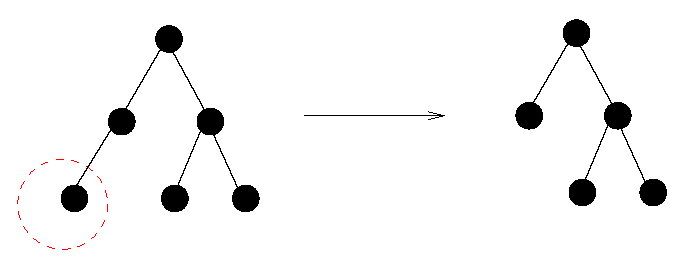
\includegraphics[width=5cm]{deleteleaf} \\ [0.5em]
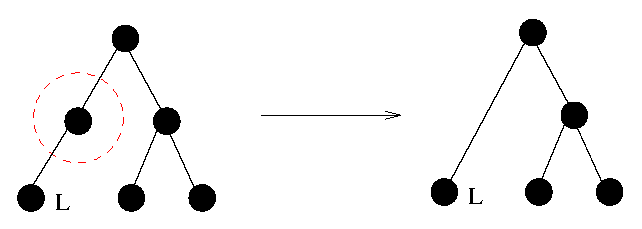
\includegraphics[width=5cm]{deletenoright} \\ [0.5em]
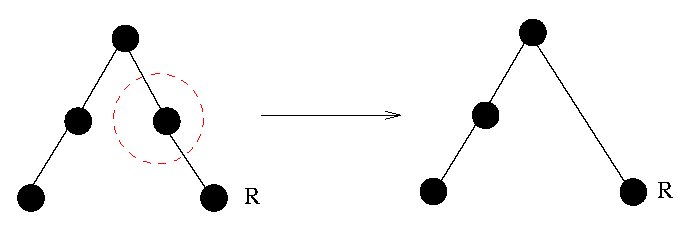
\includegraphics[width=5cm]{deletenoleft}
\end{center}
\caption{Deletion of BST nodes: easy cases.}
\label{f:bstdel}
\end{figure}
If $R(w)=\varnothing$ and $L(w)\not=\varnothing$, replace $w$ with
$L(w)$ (Fig.~\ref{f:bstdel}, middle).
\begin{ex}
Prove that this case of deletion (Fig.~\ref{f:bstdel}, middle)
satisfies Eq.~\eqref{eq:BST}.
\end{ex}
Similarly, if $L(w)=\varnothing$ and $R(w)\not=\varnothing$, replace
$w$ with $R(w)$ (Fig.~\ref{f:bstdel}, right).  Of course ``replacing''
here has a precise meaning: we define first the utility function {\tt
  unlink($w$)}:\index{unlink} applied to node $w$, this function
completely disconnects $w$ from the tree.
\begin{algorithmic}[1]
\STATE let $P(w)=${\tt null}
\STATE let $L(w)=${\tt null}
\STATE let $R(w)=${\tt null}
\end{algorithmic}
Replacing node $w$ with $u$ means to connect $u$ to the same parent
and subnodes of $w$. Here is {\tt replace($w,u$)}\index{replace} (see
Fig.~\ref{f:bstrepl}).
\begin{algorithmic}[1]
  \IF{$R(P(w)) = v$}
    \STATE $R(P(w))\leftarrow u$ {\tt // $u$ is a right subnode}
  \ELSE
    \STATE $L(P(w))\leftarrow u$ {\tt // $u$ is a left subnode}
  \ENDIF
  \IF {$u\not=\varnothing$}
    \STATE $P(u)\leftarrow P(w)$
  \ENDIF
  \STATE {\tt unlink($w$)}
\end{algorithmic}

\begin{figure}[!ht]
\begin{center}
\begin{tabular}{ccc}
\begin{minipage}{4cm}
\begin{tikzpicture}[scale=0.7]
\node (w) at (0,2) {$z$};
\node (v) at (1,1) {$w$} edge [<-] (w);
\node (u) [circle,fill=cyan!30] at (2,0) {$u$};
\end{tikzpicture}
\end{minipage}
\hfill $\longrightarrow$ \hfill
\begin{minipage}{4cm}
\begin{tikzpicture}[scale=0.7]
\node (w) at (0,2) {$z$};
\node (v) [circle,color=red,draw] at (1,1) {\color{red} $w$};
\node (u) [circle,fill=cyan!30] at (2,0) {$u$} edge 
  [bend right,color=blue,thick,<-] (w);
\end{tikzpicture}
\end{minipage}
\end{tabular}
\end{center}
\caption{Replacing a node $w$ with a node $u$.}
\label{f:bstrepl}
\end{figure}

\subsubsection{Deleting a node with both subnodes}
If $w$ has 2 non-null subnodes, deletion\index{BST!deletion!two
  subnodes} becomes slightly more complicated. We swap the value of
$w$ and of the minimum element $u$ of the right
subtree\index{subtree!right} of $w$ and then delete $u$, which ends up
being one of the easy deletion cases above, since it has a {\tt null}
left subnode. Here is {\tt replaceValueMinRight($w$)}, which returns
the node $u$ to be subsequently deleted.
\begin{algorithmic}[1]
\STATE $T'=$right subtree rooted at $w$
\STATE $u=\min T'$
\STATE swap the values of $w$ and $u$
\RETURN $u$
\end{algorithmic}
To show that this works, we have to show that Eq.~\eqref{eq:BST} holds
in the resulting BST. By Eq.~\eqref{eq:BST}, the minimum element of a
BST\index{BST!minimum} is always the leftmost
node\index{node!leftmost} without a left subtree.\index{subtree!left}

\begin{ex}
Prove the previous statement.
\end{ex}

Since $u$ is in the right subtree of $w$, by Eq.~\eqref{eq:BST}
$u>w$ and also $u$ is greater than all the elements in the left
subtree of $w$. Also, since $u$ is minimum in the right subtree, $u$
is smaller than all other elements of the right subtree. So replacing
$w$ with $u$ yields a BST where the new root\index{BST!root} is
greater than (or equal to) all nodes in its left
subtree,\index{subtree!left} and smaller than all nodes in its right
subtree.\index{subtree!right} Thus Eq.~\eqref{eq:BST} holds in the new
BST.

\begin{ex}
Are there any other possibilities for deleting $v$ from a BST in such
a way that Eq.~\eqref{eq:BST} holds?
\end{ex}

\subsubsection{Putting it all together}
Here is the code for {\tt delete($w,v$)},\index{BST!delete} which
deletes element $w$ from the tree rooted at $v$.
\begin{algorithmic}[1]
  \IF{$w<v$}
    \STATE {\tt delete}$(w,L(v))$;
  \ELSIF{$w>v$}
    \STATE {\tt delete}$(w,R(v))$;
  \ELSE 
    \STATE {\tt // base case of recursion, $w=v$}
    \IF{$L(v)=\varnothing \land R(v)=\varnothing$}
      \STATE {\tt unlink($v$)}
    \ELSIF{$L(v)=\varnothing\land R(v)\not=\varnothing$}
      \STATE {\tt replace($v,R(v)$)}
    \ELSIF{$L(v)\not=\varnothing\land R(v)=\varnothing$}
      \STATE {\tt replace($v,L(v)$)}
    \ELSE
      \STATE $u=${\tt replaceValueMinRight($v$)}
      \STATE {\tt delete($u,v$)} {\tt // an easy case}
    \ENDIF
  \ENDIF
\end{algorithmic}

\begin{eg}
In order to delete the element $10$ from the tree rooted at $r$, we
call {\tt delete($10,r$)} on the following tree.
\begin{center}
\begin{tabular}{cccc}
\begin{tikzpicture}[scale=1]
\node (v1) [circle,fill=cyan!30] at (1,2) {10};
\node (v2) at (0,1) {5} edge [<-] (v1);
\node (v3) at (0.5,0) {7} edge [<-] (v2);
\node (v4) at (2,1) {14} edge [<-] (v1);
\node (v5) at (1.5,0) {12} edge [<-] (v4);
\node (v6) at (2.5,0) {18} edge [<-] (v4);
\end{tikzpicture}
&
\begin{tikzpicture}[scale=1]
\node (v1) [fill=red!30] at (1,2) {10};
\node (v2) at (0,1) {5} edge [<-] (v1);
\node (v3) at (0.5,0) {7} edge [<-] (v2);
\node (v4) at (2,1) {14} edge [<-] (v1);
\node (v5) [circle,draw] at (1.5,0) {12} edge [<-] (v4);
\node (v6) at (2.5,0) {18} edge [<-] (v4);
\end{tikzpicture}
&
\begin{tikzpicture}[scale=1]
\node (v1) [circle,draw] at (1,2) {12};
\node (v2) at (0,1) {5} edge [<-] (v1);
\node (v3) at (0.5,0) {7} edge [<-] (v2);
\node (v4) at (2,1) {14} edge [<-] (v1);
\node (v5) [fill=red!30] at (1.5,0) {10} edge [<-] (v4);
\node (v6) at (2.5,0) {18} edge [<-] (v4);
\end{tikzpicture}
&
\begin{tikzpicture}[scale=1]
\node (v1) [fill=red!30] at (1,2) {12};
\node (v2) at (0,1) {5} edge [<-] (v1);
\node (v3) at (0.5,0) {7} edge [<-] (v2);
\node (v4) at (2,1) {14} edge [<-] (v1);
\node (v6) at (2.5,0) {18} edge [<-] (v4);
\end{tikzpicture} \\
The tree & Minimum elt. & Swap values & Delete $u$
\end{tabular}
\end{center}
\end{eg}

\subsection{Complexity}
All the recursive methods for BSTs have worst-case complexity
proportional to the length of the longest path\index{path!longest}
from the root\index{root} to a leaf.\index{leaf} If the tree is
balanced, this is $O(\log n)$, otherwise it is $O(n)$. Notice we
supplied no method for balancing a BST\index{BST!balancing}
yet. Inserting $1,3,6,7$ in an empty BST in this order yields the
unbalanced BST in Fig.~\ref{f:bstunb}.
\begin{figure}[!ht]
\begin{center}
\begin{tikzpicture}
\Tree [.1 $\varnothing$ [.3 $\varnothing$ [.6 $\varnothing$ 7 ] ] ]
\end{tikzpicture}
\end{center}
\caption{An unbalanced BST.}
\label{f:bstunb}
\end{figure}

\section{AVL trees}
Adelson-Velskii-Landis\index{Adelson}\index{Velksii}\index{Landis}
(AVL)\index{AVL} trees\index{tree!AVL} are BSTs\index{BST} with a
mechanism for balancing the tree.\index{tree!balancing} For a BST
$T$ rooted at $v$, we let $B_T(v)$ be the depth difference between
left and right subtrees of $T$ rooted at $v$ (we drop the subscript
$T$ when it is clear from the context):
\begin{equation*}
  B_T(v) = D(L(v))-D(R(v)).
\end{equation*}
An AVL tree $T$ always has the following property:
\begin{equation}
  \forall v\in T \; B_T(v)\in\{-1,0,1\}. \label{eq:AVL}
\end{equation}
This means that $B(r(T))$ is $O(1)$ (asymptotics on the number $n$ of
nodes in the BST), which implies that all recursive BST methods are
$O(\log n)$.

\begin{ex}
Prove formally that in a BST with $n$ nodes, Eq.~\eqref{eq:AVL} yields a
maximum root$\to$leaf path length of $\log n$.
\end{ex}

\begin{eg}
Here are examples of AVL and non-AVL BSTs. The nodes are labelled with
$B(v)$.
\begin{center}
\begin{tabular}{cc}
\begin{tikzpicture}
\Tree [.$-1$ [.$1$ [.$1$ $0$ $0$ ]
    $0$ ] [.$-1$ [.$-1$ $0$ [.$1$
        $0$ $\varnothing$ ] ] [.$0$ [.$-1$ $\varnothing$ $0$ ] [.$0$
        $0$ $0$ ] ] ] ]
\end{tikzpicture}
&
\begin{tikzpicture}
\Tree [.$-2$ $0$ [.$-1$ $0$ [.$-1$ $\varnothing$ $0$ ] ] ]
\end{tikzpicture} \\ 
AVL tree & non-AVL tree
\end{tabular}
\end{center}
\end{eg}

\subsection{Balance-independent methods}
The methods {\tt min},\index{min} {\tt max},\index{max} {\tt
  find}\index{find} do not change the BST, so if Eq.~\eqref{eq:AVL}
holds before the call, it also holds after the call.

\subsection{Balance-dependent methods}
The methods {\tt insert}\index{insert} and {\tt delete}\index{delete}
either add or remove a node from the BST. This means that if
Eq.~\eqref{eq:AVL} holds before the call, after the call we might have
$B(v)\in\{-2,-1,0,1,2\}$. In this section we introduce methods for
rebalancing based on tree rotation.\index{tree!rotation}

We consider a BST rooted at $u$, with a left subtree called $\alpha$,
and right subtree rooted at $v=R(u)$, which itself has a left subtree
called $\beta$ and a right subtree called $\gamma$. A {\it left
  rotation}\index{rotation!left} rearranges the arcs so that the BST
is rooted at $v$, its right subtree is $\gamma$, and its left subtree
is rooted at $u$, with has left subtree $\alpha$ and right subtree
$\beta$, as shown in Fig.~\ref{f:rotate}. The {\it right
  rotation}\index{rotation!right} is the inverse\index{inverse}
transformation.
\begin{figure}[!ht]
\begin{center}
\psfrag{u}{$u$}
\psfrag{v}{$v$}
\psfrag{a}{$\alpha$}
\psfrag{b}{$\beta$}
\psfrag{g}{$\gamma$}
\psfrag{rotLeft}{$\mbox{\tt rotateLeft}$}
\psfrag{rotRight}{$\mbox{\tt rotateRight}$}
\includegraphics[width=10cm]{rotate}
\end{center}
\caption{{\tt rotateLeft} transforms the left BST\index{BST!left} $T$
  into the right one $T'$. {\tt rotateRight} transforms the right
  BST\index{BST!right} $T'$ into the left one $T$.}
\label{f:rotate}
\end{figure}
The operation of rotating a BST\index{BST!rotating} is such that:
\begin{enumerate}
\item it is invariant with respect to the BST
  property\index{BST!property} (Eq.~\eqref{eq:BST});
\item If $B_T(u)=-2$, then $B_{T'}(v)=0$; if $B_{T'}(v)=2$, then
  $B_{T}(u)=0$.
\end{enumerate}
Thus, it can be used for rebalancing BSTs\index{BST!rebalancing}
having a shape\index{tree!shape} like $T$ or $T'$.

\subsubsection{Tree rotation properties}
In order to prove the properties above, we introduce an algebraic
notation for BSTs: we let a BST rooted\index{BST!rooted} at $r$ be
denoted by $\langle L(r),r,R(r)\rangle$. For example, the left BST in
Fig.~\ref{f:rotate} is
$T=\langle\alpha,u,\langle\beta,v,\gamma\rangle\rangle$, and the right
one is $T'=\langle\langle\alpha,u,\beta\rangle,v,\gamma\rangle$. Thus,
we have
\begin{itemize}
\item $\mbox{\tt rotateLeft}(T)=T'$ 
\item $\mbox{\tt rotateRight}(T')=T$
\end{itemize}
Directly by definition, we infer that $\mbox{\tt
  rotateRight}(\mbox{\tt rotateLeft}(T))=\mbox{\tt
  rotateLeft}(\mbox{\tt rotateRight}(T))=T$.

\begin{prop}
If $T$ is a BST, $\mbox{\tt rotateLeft}(T)$, $\mbox{\tt
  rotateRight}(T')$ are BSTs, i.e.~they satisfy Eq.~\eqref{eq:BST}.
\end{prop}
\begin{proof}
The node order\index{node!order} in the tree only changes for $u$ and
$v$. In $T$, $v=R(u)$, which by Eq.~\eqref{eq:BST} implies $u<v$. In
$\mbox{\tt rotateLeft}(T)$, $u=L(v)$, which also implies $u<v$. The
proof for $T'$ is similar.
\end{proof}

Now suppose that the depths\index{depth} of $\alpha,\beta$ is $h$, and
the depth of $\gamma$ is $h+1$. Then the depth
difference\index{depth!difference} $B(u)$ of the tree
$\langle\alpha,u,\langle\beta,v,\gamma\rangle\rangle$ is $-2$, and,
similarly, $B(v)=2$.

\begin{prop}
$B(r(\mbox{\tt rotateLeft}(T)))=B(r(\mbox{\tt rotateRight}(T')))=0$.
\label{prop:rot}
\end{prop}

\begin{ex}
A proof sketch for Prop.~\ref{prop:rot} is that since the
subtrees\index{subtree} $\alpha,\gamma$ are swapped, and those
subtrees are the cause of the unbalance,\index{unbalance} the rotated
tree is balanced. Formalize this proof sketch.
\end{ex}

\subsubsection{The remaining cases}
Consider the case of a tree\index{tree}
$S=\langle\alpha,u,\langle\beta,v,\gamma\rangle\rangle$ where
$D(r(\alpha))=D(r(\beta))=h$, and $D(r(\gamma)=h+1$. This does not
fall into either of the cases $T,T'$ above. Because $\gamma$ is the
left subtree\index{subtree!left} of $v$, it has depth $h+3$, while the
depth of $\alpha$ is $h+1$, so $B_S(u)=-2$ and the tree is unbalanced
(see Fig.~\ref{f:rc}).\index{tree!unbalanced} Rotating $S$, however,
only exchanges the roles of $\alpha,\beta$, fixing $\gamma$; this
results in another unbalanced tree.
\begin{figure}[!ht]
\begin{center}
\begin{center}
\psfrag{u}{$u$}
\psfrag{v}{$v$}
\psfrag{D}{$D=h$}
\psfrag{D1}{$D=h+1$}
\psfrag{B2}{\color{darkred} $-2$}
\psfrag{B1}{\color{darkgreen} $1$}
%\psfrag{B0}{\scriptsize\color{darkgreen} $0$}
\psfrag{a}{$\alpha$}
\psfrag{b}{$\beta$}
\psfrag{g}{$\gamma$}
\includegraphics[width=5cm]{midcase}
\end{center}
\end{center}
\caption{The unbalanced tree shape $S$.}
\label{f:rc}
\end{figure}
To deal with tree shape $S$, we ``break up'' the subtree $\gamma$,
writing it as $\langle\lambda,r(\gamma),\mu\rangle$ . Assume first
that $\lambda$ has depth $h$ and $\mu$ has depth $h-1$, as shown in
Fig.~\ref{f:remcase}, so that $B(r(\gamma))=1$, and call this tree
shape $S'$.
\begin{figure}[!ht]
\begin{center}
\psfrag{u}{$u$}
\psfrag{v}{$v$}
\psfrag{D}{\small $D=h$}
\psfrag{h}{\small $h$}
\psfrag{h-1}{\small $h-1$}
\psfrag{B2}{\small \color{darkred} $-2$}
\psfrag{B1}{\small \color{darkgreen} $1$}
\psfrag{a}{$\alpha$}
\psfrag{b}{$\beta$}
\psfrag{g}{$\gamma$}
\psfrag{l}{$\lambda$}
\psfrag{m}{$\mu$}
\includegraphics[width=5cm]{midcase2}
\end{center}
\caption{The unbalanced tree shape $S'$.}
\label{f:remcase}
\end{figure}
We now recognize the BST rooted\index{BST!rooted} at $v$ as a tree of
shape\index{tree!shape} $T'$. Although it is not
unbalanced\index{unbalance} itself, as $B(v)=1$, we rotate it
right:\index{rotation!right} the effect of this operation will be to
``shift'' the unbalance of the tree shape $S'$ from the subtree
$\gamma$ to the subtree\index{subtree} $\beta$. Thereafter, the
resulting BST will be still unbalanced but will have shape $S$, and a
left rotation\index{rotation!left} will balance it (see
Fig.~\ref{f:leftrightrot}).
\begin{figure}[!ht]
\begin{center}
\psfrag{u}{$u$}
\psfrag{v}{$v$}
\psfrag{D}{\scriptsize $D=h$}
\psfrag{D1}{\scriptsize $D=h+1$}
\psfrag{h}{\scriptsize $h$}
\psfrag{h-1}{\scriptsize $h-1$}
\psfrag{B2}{\scriptsize\color{darkred} $-2$}
\psfrag{B1}{\scriptsize\color{darkgreen} $1$}
\psfrag{B1p}{\scriptsize\color{darkgreen} $-1$}
\psfrag{Bv}{\scriptsize\color{darkgreen} $-1$}
%\psfrag{B0}{\scriptsize\color{darkgreen} $0$}
\psfrag{a}{$\alpha$}
\psfrag{b}{$\beta$}
\psfrag{g}{$\gamma$}
\psfrag{rg}{$r(\gamma)$}
\psfrag{rotRightSub}{\scriptsize $\mbox{\tt rotateRight}(\mbox{\sf R}(u))$}
\includegraphics[width=12cm]{midcase3}  \\ [-1em] $\swarrow$ \\ [-0.5em]
\psfrag{u}{$u$}
\psfrag{v}{$v$}
\psfrag{D}{\scriptsize $D=h$}
\psfrag{D1}{\scriptsize $D=h+1$}
\psfrag{h}{\scriptsize $h$}
\psfrag{h-1}{\scriptsize $h-1$}
\psfrag{B2}{\scriptsize \color{darkred} $-2$}
\psfrag{B1}{\scriptsize \color{darkred} $-2$}
\psfrag{B1}{\scriptsize \color{darkgreen} $-1$}
\psfrag{B0}{\scriptsize\color{darkgreen} $0$}
\psfrag{Bu}{\scriptsize\color{darkgreen} $0$}
\psfrag{Bv}{\scriptsize\color{darkgreen} $-1$}
\psfrag{a}{$\alpha$}
\psfrag{b}{$\beta$}
\psfrag{g}{$r(\gamma)$}
\psfrag{rotateLeft}{\scriptsize $\mbox{\tt rotateLeft}(T)$}
\includegraphics[width=13cm]{midcase4}
\end{center}
\caption{Dealing with tree shape\index{tree!shape} $S'$: a right
  rotation\index{rotation!right} of the right subtree\index{subtree!right}
  followed by a left rotation\index{rotationa!left} of the result
  rebalances the BST.\index{BST}}
\label{f:leftrightrot}
\end{figure}

Another tree shape $S''$, which has $\lambda$ with depth $h-1$ and
$\mu$ with depth $h$, is symmetric with respect to $S'$ and can be
handled in exactly the same way, i.e.~right rotation of the right
subtree of the root, followed by a left rotation of the resulting
BST (Fig.~\ref{f:lrsymm}).
\begin{figure}[!ht]
\begin{center}
\psfrag{u}{$u$}
\psfrag{v}{$v$}
\psfrag{D}{\scriptsize $D=h$}
\psfrag{D1}{\scriptsize $D=h+1$}
\psfrag{h}{\scriptsize $h$}
\psfrag{h-1}{\scriptsize $h-1$}
\psfrag{B2}{\scriptsize \color{darkred} $-2$}
\psfrag{B1}{\scriptsize \color{darkgreen} $1$}
\psfrag{B1p}{\scriptsize \color{darkred} $-2$}
\psfrag{Bv}{\scriptsize\color{darkgreen} $0$}
%\psfrag{B0}{\scriptsize\color{darkgreen} $0$}
\psfrag{a}{$\alpha$}
\psfrag{b}{$\beta$}
\psfrag{g}{$\gamma$}
\psfrag{rg}{$r(\gamma)$}
\psfrag{rotRightSub}{\scriptsize $\mbox{\tt rotateRight}(\mbox{\sf R}(u))$}
\includegraphics[width=12cm]{midcase3symm} \\ [-1em] $\swarrow$ \\ [-0.5em]
\psfrag{u}{$u$}
\psfrag{v}{$v$}
\psfrag{D}{\scriptsize $D=h$}
\psfrag{D1}{\scriptsize $D=h+1$}
\psfrag{h}{\scriptsize $h$}
\psfrag{h-1}{\scriptsize $h-1$}
\psfrag{B2}{\scriptsize \color{darkred} $-2$}
\psfrag{B1}{\scriptsize \color{darkgreen} $0$}
\psfrag{B0}{\scriptsize\color{darkgreen} $0$}
\psfrag{Bu}{\scriptsize\color{darkgreen} $1$}
\psfrag{Bv}{\scriptsize\color{darkgreen} $0$}
\psfrag{a}{$\alpha$}
\psfrag{b}{$\beta$}
\psfrag{g}{$r(\gamma)$}
\psfrag{rotateLeft}{\scriptsize $\mbox{\tt rotateLeft}(T)$}
\includegraphics[width=13cm]{midcase4symm}
\end{center}
\caption{Tree shape $S''$, symmetric with $S'$ and handled in the same
way.}
\label{f:lrsymm}
\end{figure}

A last unbalanced tree shape $\bar{S}$ rooted at $u$ needs
handling. This is symmetric with $S$, having $B(u)=2$ (see
Fig.~\ref{f:lrsymm2}).
\begin{figure}[!ht]
\begin{center}
\psfrag{u}{$u$}
\psfrag{v}{$v$}
\psfrag{D}{$D=h$}
\psfrag{D1}{$D=h+1$}
\psfrag{B2}{\color{darkred} $2$}
\psfrag{B1}{\color{darkgreen} $-1$}
%\psfrag{B0}{\scriptsize\color{darkgreen} $0$}
\psfrag{a}{$\alpha$}
\psfrag{b}{$\beta$}
\psfrag{g}{$\gamma$}
\includegraphics[width=5cm]{midcasesymm1}
\end{center}
\caption{The unbalanced tree shape $\bar{S}$.}
\label{f:lrsymm2}
\end{figure}
Following the same pattern as above, we can distinguish two further
symmetric unbalanced tree\index{tree!unbalanced}
shapes\index{tree!shape}\index{tree!shape!symmetric}
$\bar{S}',\bar{S}''$, both subsumed by $\bar{S}$. Both can be
rebalanced in the same way, by rotating $L(u)$ left first, and then
rotating the resulting BST right.

\begin{ex}
Convince yourself that $T,T',S,\bar{S}$ exhaust the possible tree
shapes\index{tree!shape} that can occur after an {\tt
  insert}\index{BST!insert} or {\tt delete}\index{BST!delete}
operation in a BST.\index{BST} 
\end{ex}

\section{Heaps}
\label{s:search:heap}
A {\it heap}\index{heap} is a basic tree-like data
structure\index{data!structure!tree-like} that is specially conceived
to implement the concept of a {\it priority queue}
efficiently.\index{queue!priority} 

\subsection{Priority queues}
\label{s:search:heap:priorityq}
A priority queue is simply a queue\index{queue} (see
Sect.~\ref{s:linear:queue}) with an additional node
extraction\index{node!extraction} mechanism. Specifically, we
associate a scalar\index{scalar} $p(v)$ (called {\it
  priority})\index{priority} to each element $v$ of the queue $V$, and
want to be able to efficiently extract an element from highest
priority.\index{priority!highest} Accordingly, we introduce two new
methods to the queue's standard set of methods: {\tt max}\index{max}
and {\tt popMax}.\index{popMax@{\tt popMax}} The former returns the priority
of the element with highest priority, and the latter returns the
element of highest priority and removes it from $V$. We also modify
{\tt insert($v,p(v)$)} to also take the priority of $v$ as input.

\begin{ex}
Show that, if $p(v)$ is an integer specifying the order of entrance in
the queue, {\tt popMax} has the same effect as the {\tt
  popFront}\index{popFront@{\tt popFront}} method in standard queues.
\end{ex}

\subsection{Heap properties}
Having motivated heaps, we now look at them in more depth. A
heap\index{heap} is a binary tree\index{tree!binary} with the
following properties.
\begin{enumerate}
\item All tree levels\index{tree!level} except perhaps the last one
  are fully filled; the last one is filled left-to-right ({\it shape
    property}).\index{heap!shape property}
\item Every node stores an element of higher property than its
  subnodes ({\it heap property}).\index{heap!property}
\end{enumerate}
We remark that a heap\index{heap} is not a BST,\index{BST} as
Eq.~\eqref{eq:BST} is not necessarily satisfied.

Intuitively, the shape property ensures that the tree is
balanced,\index{tree!balanced} and hence most
depth-dependent\index{method!depth-dependent} methods are $O(\log n)$
instead of $O(n)$ (where $n=|V|$). The heap property induces the
element of $V$ having highest priority\index{priority!highest} to be
stored as the root node.\index{node!root}

\begin{eg}
An example of heap where $V\subseteq\mathbb{N}$ and the priority order
is simply the usual integer order.
\begin{center}
\begin{tikzpicture}
\Tree [.100 [.19 [.17 2 7 ] 3 ] [.36 25 1 ] ]
\end{tikzpicture}
\end{center}
\end{eg}

\begin{prop}
If $V$ is a heap, $\forall v\in V\; B_V(v)\in\{0,1\}$.
\end{prop}
\begin{proof}
This follows trivially from the shape property.\index{heap!shape
  property} Since all levels\index{level} are filled completely apart
perhaps from the last, $B(Q)\in\{-1,0,1\}$. Since the last is filled
left-to-right, $B(Q)\not=-1$.
\end{proof}
Thus, a heap\index{heap} is a balanced binary
tree.\index{tree!binary!balanced} Since a heap is not a BST\index{BST}
(and thus not an AVL tree),\index{tree!AVL} we cannot use the same
balanced insertion and deletion methods as for AVL trees.

Notice that the shape property\index{heap!shape property} induces a
linear order\index{order!linear} $\prec$ on the heap
nodes,\index{heap!node} based on levels: for two nodes $u,v$ in a
heap, we let $u\prec v$ if and only if either the
depth\index{node!depth} of $u$ is smaller than the depth of $v$, or,
if $u,v$ are on the same level,\index{heap!level} if $u$ is on the
left\index{left} of $v$. This order defines a notion of
$\prec$-successor,\index{successor} which can also be extended to the
$\prec$-last element in the heap:\index{heap!last} the
$\prec$-successor position after the $\prec$-last element is either
the leftmost ``free slot'' in the last level, if this is not
completely filled,\index{tree!level!filled} or the leftmost slot in a
new level otherwise. This position is also called the {\it bottom of
  the heap}.\index{heap!bottom}

\subsubsection{Insertion}
In order to add a new element $v$ with priority $p(v)$ to the heap
$V$, we insert it at the bottom of the heap,\index{heap!bottom} then
``float it up'' the path to the root\index{root!path to} while its
priority\index{priority!higher} is higher than that of its
parent.\index{parent} Here is the code for {\tt
  floatUp($v$)},\index{heap!floatUp@{\tt floatUp}} which floats a node $v$ up
a heap $V$ rooted at $r$, until $v$'s position satisfies the heap
property.\index{heap!property}
\begin{algorithmic}[1]
\WHILE{$v\not=r\land p(v)>p(P(v))$}
  \STATE swap $v$ with $P(v)$
\ENDWHILE
\end{algorithmic}

\begin{eg}
As an example, we insert $1,4,2,3,5$ in an empty heap. 
\begin{center}
\begin{tabular}{|c|c|c|c|c|c|c|c|c|c|} \hline
\begin{tikzpicture}
\Tree [.$\varnothing$ ]
\end{tikzpicture}
&
\begin{tikzpicture}
\Tree [.$1$ ]
\end{tikzpicture}
&
\begin{tikzpicture}
\Tree [.$1$ $4$ $\varnothing$ ]
\end{tikzpicture}
&
\begin{tikzpicture}
\Tree [.\fbox{\color{darkblue}$4$} \fbox{\color{darkblue}$1$} $\varnothing$ ]
\end{tikzpicture}
&
\begin{tikzpicture}
\Tree [.$4$ $1$ $2$ ]
\end{tikzpicture}
&
\begin{tikzpicture}
\Tree [.$4$ [.$1$ $3$ $\varnothing$ ] $2$ ]
\end{tikzpicture}
&
\begin{tikzpicture}
\Tree [.$4$ [.\fbox{\color{darkblue}$3$} \fbox{\color{darkblue}$1$}
    $\varnothing$ ] $2$ ]
\end{tikzpicture}
&
\begin{tikzpicture}
\Tree [.$4$ [.$3$ $1$ $5$ ] $2$ ]
\end{tikzpicture}
&
\begin{tikzpicture}
\Tree [.$4$ [.\fbox{\color{darkblue}$5$} $1$ \fbox{\color{darkblue}$3$} ] $2$ ]
\end{tikzpicture}
&
\begin{tikzpicture}
\Tree [.\fbox{\color{darkblue}$5$} [.\fbox{\color{darkblue}$4$} $1$ $3$ ] $2$ ]
\end{tikzpicture}
\\ \hline
 & insert $1$ & insert $4$ & float $4$ & insert $2$ & insert $3$ &
float $3$ & insert $5$ & float $5$ & float $5$ 
\\ \hline
\end{tabular}
\end{center}
\label{eg:newheap}
\end{eg}

\begin{ex}
Write {\tt floatUp} as a recursive algorithm.\index{algorithm!recursive}
\end{ex}

\begin{ex}
Prove that heap insertion\index{heap!insertion} maintains the
shape\index{heap!shape properties} and heap
properties.\index{heap!property}
\end{ex}

Because a heap is a balanced tree, insertion takes $O(\log n)$.

\subsubsection{Maximum}
Returning the highest prority\index{priority!highest} over all heap
elements is equivalent to simply returning the priority of the root
element,\index{root!priority} because of the {\tt floatUp}\index{floatUp@{\tt
    floatUp}} operation. Obviously, the complexity of the {\tt
  max}\index{max} method is $O(1)$.

\subsubsection{Popping the maximum}
\label{s:search:heap:popmax}
Since the highest priority\index{priority!highest} element is at the
root of the heap,\index{heap!root} we save the root for returning it
later. We then overwrite the root with the $\prec$-last heap element,
i.e.~the rightmost ``filled slot'' on the last heap
level,\index{heap!level} and unlink\index{heap!unlink} the latter (the
{\tt unlink}\index{unlink} method can be borrowed from BSTs). Finally,
we float\index{heap!float} the updated root down the heap while one of
its subnodes have higher priority.\index{priority!higher} Here is the
{\tt floatDown($v$)}\index{floatDown@{\tt floatDown}} method.
\begin{algorithmic}[1]
\WHILE{$v<\max(L(v),R(v))$}
  \STATE swap $v$ with $\max(L(v),R(v))$
\ENDWHILE
\end{algorithmic}
In {\tt floatDown}, we assume that if $v$ has no left subnode, then
$L(v),R(v)$ return $\varnothing$, and that $\varnothing$ has priority
$-\infty$.

\begin{eg}
Here is an example of popping the maximum element from the
heap.\index{heap!popMax@{\tt popMax}}
\begin{center}
\begin{tabular}{|c|c|c|c|}\hline
\begin{tikzpicture}
\Tree [.$5$ [.$4$ $1$ $3$ ] $2$ ]
\end{tikzpicture} &
\begin{tikzpicture}
\Tree [.$5$ [.$4$ $1$ \fbox{$3$} ] $2$ ]
\end{tikzpicture} &
\begin{tikzpicture}
\Tree [.\fbox{$3$} [.$4$ $1$ $\varnothing$ ] $2$ ]
\end{tikzpicture} &
\begin{tikzpicture} 
\Tree [.\fbox{\color{darkblue}$4$} [.\fbox{\color{darkblue}$3$} $1$
    $\varnothing$ ] $2$ ] 
\end{tikzpicture} \\ \hline
heap & $\prec$-last & move to root & swap with $L(r)$ 
\\ \hline
\end{tabular}
\end{center}
\end{eg}
The {\tt floatDown} operation takes $O(\log n)$ in the
worst case, so {\tt popMax} also takes $O(\log n)$.

\begin{ex}
Prove that {\tt floatDown} preserves the shape property.
\label{ex:fd}
\end{ex}

\subsubsection{Initial heap construction}
In Example \ref{eg:newheap}, we constructed a new heap\index{heap!new}
by inserting all the element in an empty heap,\index{heap!empty} one
after the other. This has complexity $O(n\log n)$, since we must
insert $n$ element, and each insertion\index{insertion} takes $O(\log
n)$. This is suboptimal; consider the following procedure instead.
\begin{enumerate}
\item Insert elements in a binary tree\index{tree!binary} $V$ in their
  natural order,\index{order!natural} respecting the
  shape\index{shape!property} property but not the heap
  property.\index{heap!property}
\item For each $v\in V$, call {\tt floatDown($v$)}.
\end{enumerate}
It should be obvious that the net effect of the above procedure is the
same as inserting elements in a heap one by one, since the first step
ensures the shape property is satisfied, whilst the second ensures the
heap property is satisfied (by Exercise \ref{ex:fd}, the shape
property is preserved).

A superficial worst-case analysis gives the above procedure at
$O(n\log n)$: there are $n$ elements, and each {\tt floatDown} costs
$O(\log n)$ by Sect.~\ref{s:search:heap:popmax}. There is a more
refined analysis, however. The {\tt floatUp($v$)}\index{floatUp@{\tt floatUp}}
and {\tt floatDown($v$)}\index{floatDown@{\tt floatDown}} methods take a CPU
time proportional to the level\index{tree!level} $\ell$ of the
node\index{node!level} $v$. There are at most
$\lceil\frac{n}{2^{\ell+1}}\rceil$ nodes at level $\ell$, and $O(\log
n)$ possible levels. Thus, the overall worst-case complexity is:
\begin{eqnarray*}
  \sum_{\ell=0}^{\lceil\log n\rceil}\frac{n}{2^{\ell+1}} O(\ell) &=& 
  O\left(n \sum_{\ell=0}^{\lceil\log n\rceil}\frac{1}{2^{\ell}}\right) \\
  &\le& O\left(n \sum_{\ell=0}^{\infty}\frac{1}{2^{\ell}}\right) \\
  &=& O(2n) \\ &=& O(n).
\end{eqnarray*}

\begin{ex}
Implement a Java heap with the following methods: {\tt insert($v$)}, {\tt
  max()}, {\tt popMax()}. Implement the two versions of {\tt
  initialize($V$)} given in this section, and compare the CPU time
they take over sets of 10, 100, 1000, 10000, 100000 elements. Do your
empirical observations fit the theory?
\end{ex}


%%%%%%%%%%%%%%%%% CHAPTER: SHORTEST PATHS %%%%%%%%%%%%%%%%%%%%
\chapter{Shortest paths}
\label{c:path}

\begin{center}
\fbox{\begin{minipage}{13cm}{\small {\sc Abstract}.  Shortest path
      problems and variants. Negative weights and negative
      cycles. Dijkstra's algorithm: simple and more refined
      pseudocodes, with complexity. Floyd-Warshall's algorithm.}
\end{minipage}}
\end{center}

Given an edge-weighted\index{edge!weighted} directed or undirected
graph,\index{graph!directed}\index{graph!undirected} the problem of
finding shortest paths\index{path!shortest} in the graph, in terms of
the sum of the weights\index{weight!sum} of the path
edges,\index{path!edge} has dozens of applications, in
logistics,\index{logistics} communication
networks,\index{network!communication} power
networks,\index{network!power} engineering,\index{engineering},
computer science\index{computer science} itself (shortest path
computations are often sub-steps\index{algorithm!sub-step} of more
complex algorithms), and other fields.

Although in digraphs\index{digraph} paths\index{path} are technically
known as walks,\index{walk} in this chapter we shall nonetheless call
them paths for historical reasons. Similarly, we use the term
cycle\index{cycle} to possibly mean a circuit\index{circuit} in a
digraph. Moreover, undirected graphs occurring in path problems can be
replaced by digraphs with pairs of antiparallel arcs $(u,v)$ and
$(v,u)$ for every edge $\{u,v\}$ in the original graph $G$. 

In the rest of this chapter, we assume that all graphs are
connected,\index{graph!connected} and that digraphs are strongly
connected.\index{digraph!strongly connected}


\section{Basic literature}
\label{s:path:literature}

\subsection{Problem variants}
Although the concept of a shortest path is easy to grasp, there are
several different formal variants of the shortest path problem. Here
are some of these.
\begin{itemize}
\item The {\sc Shortest Path Problem}\index{shortest path problem@{\sc
    Shortest Path Problem}} (SPP).\index{SPP} Given a directed or
  undirected graph\index{graph}\index{digraph} $G=(V,A)$, a node or
  vertex $s\in V$, and a non-negative arc or edge weight
  function\index{function!edge weight} $c:A\to\mathbb{R}_+$, find
  $c$-shortest paths from $s$ to all other vertices of $V$. This
  problem is in {\bf P}.
\item The SPP with unit weights\index{weight!unit} is the SPP with
  $c:A\to\{1\}$, i.e.~all arcs/edges have the same (unit) weight. This
  problem is in {\bf P}.
\item The {\sc Negative Cycle Problem}\index{cycle!negative} (NCP)
  asks to determine whether $G$ has a cycle of negative weight (the
  weigth of a cycle is the sum of the weights of the cycle edges).
  This problem is in {\bf P}.
\item The SPP with negative weights\index{weight!negative} is the SPP
  with $c:A\to\mathbb{R}$, i.e.~$c$ can also take negative values.
  This problem is in {\bf P}.
\item The {\sc Point-to-Point Shortest Path
  Problem}\index{point-to-point SPP@{\sc
    Point-to-Point SPP}} (P2PSPP).\index{P2PSPP} Given $G$, $c$, and
  two distinct nodes or vertices $s,t\in V$, find a $c$-shortest path
  from $s$ to $t$. This problem is in {\bf P}.
\item The {\sc All Shortest Paths}\index{path!all} (ASP)\index{ASP}
  problem asks to determine all shortest paths from $u$ to $v$ for any
  couple\index{couple} $(u,v)$ of nodes or vertices in $V$. This
  problem is in {\bf P}.
\item The {\sc Shortest Simple Path}\index{shortest simple path@{\sc
    Shortest Simple Path}} (SSP)\index{SSP} problem consists in
  finding the shortest simple path\index{path!simple} from $s$ to $t$
  in $G$. This problem is {\bf NP}-hard.
\item The {\sc Longest Path Problem}\index{longest path problem@{\sc
    Longest Path Problem}} (LPP)\index{LPP} asks to find the
  longest\index{path!longest} simple path\index{path!simple} from $s$
  to $t$ in $G$. This problem is {\bf NP}-hard.
\item The {\sc Undirected SPP} (USPP)\index{USPP} with weights in $N$
  requires $G$ to be an undirected graph\index{graph!undirected} and
  can be solved in linear time.\index{linear!time}
\end{itemize}

\subsection{Algorithms}
To every problem variant, there corresponds a specific algorithm. 
\begin{itemize}
\item The SPP\index{SPP} can be solved by Dijkstra's\index{Dijkstra,
  E.}  algorithm\index{algorithm!Dijkstra} (see
  Sect.~\ref{s:path:dijkstra} below), which bears some resemblance to
  the {\sc Graph Scanning}\index{graph scanning@{\sc Graph Scanning}}
  algorithm (see Sect.~\ref{s:graphalg:gphscn}) with $Q$ implemented
  as a priority queue (see Sect.~\ref{s:search:heap:priorityq}), and
  no restrictions about scanning a vertex more than
  once.\index{queue!priority} Dijkstra's algorithm runs in polynomial
  time (simple implementation: $O(n^2)$).
\item The SPP with unit weights is solved using {\sc Breadth-First
  Search}\index{breadth-first search@{\sc Breadth-First
    Search}}\index{BFS} as explained in
  Sect.~\ref{s:graphalg:bfs}. BFS runs in linear time $O(n+m)$.
\item The NCP\index{NCP} and the SPP\index{SPP} with negative
  weights\index{weight!negative}\index{SPP!negative weights} are
  related. In fact, the issue with having negative weights in the SPP
  is that the path weight might be unbounded.\index{unbounded!path
    weight} More precisely, if there is a cycle of negative
  weight,\index{cycle!negative} any path from $s$ to $t$ can travel
  along the cycle as many times as desired (notice that the path is
  not required to be simple)\index{path!simple} to reduce its weight
  as much as desired. The Bellman-Ford
  algorithm\index{algorithm!Bellman-Ford},\index{Bellman,
    R.}\index{Ford, L.} which runs in polynomial time $O(nm)$, scans
  all arcs repeatedly to identify either a shortest path
  tree\index{tree!shortest path} or identify a negative weight cycle,
  and therefore solves both the NCP and the SPP with negative weights.
\item The ASP can be solved using the Floyd-Warshall
  algorithm,\index{algorithm!Floyd-Warshall}\index{Floyd}\index{Warshall}
  which runs in polynomial time $O(n^3)$ and, interestingly, also
  solves the NCP.
\item The algorithm for solving the USPP with nonnegative integer
  weights is given in \cite{thorup}. 
\end{itemize}

The SSP\index{SSP} and LSP\index{LSP} can be solved either using brute
force, or using an implicit enumeration method, such as the {\sc
  Branch-and-Bound}\index{branch-and-bound@{\sc Branch-and-Bound}}
(BB)\index{BB} algorithm, or using heuristics\index{heuristic} (see
Sect.~\ref{s:problem:exactheur}).

\section{Weight functions}
If $F$ is a set of $c$-weighted arcs in the digraph $G=(V,A)$, the
cost function $c:A\to\mathbb{R}$ can be extended to sets of arcs by
setting
\begin{equation*}
  c(F) = \sum_{(u,v)\in F} c_{uv}.
\end{equation*}

\begin{ex}
Prove formally that, if there exist a negative weighted
circuit\index{circuit!weighted} in the digraph\index{digraph}
$G=(V,A)$, no walk\index{walk} $P=(U,F)$ attains the minimum on the
function $c$ extended to sets of arcs.
\end{ex}

\begin{eg}
The cycle emphasized in the graph below has negative weight
$1+0-4+2=-1<0$.
\begin{center}
\begin{tikzpicture}[scale=1]
\node (v1) [circle,draw] at (1,0) {$1$} ;
\node (v2) [circle,draw] at (3,0) {$2$} ;
\node (v3) [circle,draw] at (4,1) {$3$} ;
\node (v4) [circle,draw] at (3,2) {$4$} ;
\node (v5) [circle,draw] at (1,2) {$5$} ;
\node (v6) [circle,draw] at (0,1) {$6$} ;
\node (v7) [circle,draw] at (4.5,2.7) {$7$} ;
\draw (v1) to node[below] {2} (v2) ;
\draw (v1) [->,thick] to node[near end, above] {1} (v3) ;
\draw (v1) to node[right] {1} (v5) ;
\draw (v1) [<-,thick] to node[below] {2} (v6) ;
\draw (v2) to node[below] {1} (v3) ;
\draw (v2) to node[above] {1} (v5) ;
\draw (v3) [->,thick] to node[above] {0} (v4) ;
\draw (v3) to node[below] {1} (v5) ;
\draw (v3) to node[right] {5} (v7) ;
\draw (v4) [->,thick] to node[below, very near end] {-4} (v6) ;
\draw (v4) to node[below] {3} (v7) ;
\draw (v5) to node[above] {2} (v6) ;
\draw (v5) to node[above] {6} (v7) ;
\end{tikzpicture}
\end{center}
\end{eg}

If an arc weight function\index{function!arc weight}
$c:A\to\mathbb{R}$ yields no negative cycles\index{cycle!negative} on
a digraph\index{digraph} $G=(V,A)$, it is called {\it
  conservative}.\index{function!weight!conservative}

\section{The shortest path tree}\index{tree!shortest path}
Given a graph $G=(V,E)$, a conservative weight function
$c:E\to\mathbb{R}$ and a source vertex\index{vertex!source} $s\in V$,
it is not immediately evident that the union of all shortest
paths\index{path!shortest} from $s$ to all other vertices forms a
spanning tree\index{tree!spanning} of $G$. After all, two paths from
$s$ to two vertices $v,w$ might intersect at a single vertex $u$, and
thus form a cycle\index{cycle} including $s$ and $u$. This is indeed
possible; however, shortest paths need not be unique,\index{path!not
  unique} and if two shortest paths from $s$ to $v,w$ form a cycle,
then there must exist another shortest path from $s$ to $w$ which
follows the shortest path from $s$ to $v$ until $u$, and forks towards
$w$ later (and similarly for the case where $v,w$ are inverted).

\begin{thm}
If $c$ is conservative,\index{conservative} every initial
subpath\index{subpath!initial} of a shortest path is a shortest path.
\label{thm:path}
\end{thm}
\begin{proof}
Let $P$ be a shortest path from $s$ to $v$, and let $u$ be a
vertex\index{vertex} in $P$ different from $u,v$. Suppose, to get a
contradiction, that the initial subpath $P_0$ of $P$ from $s$ to $u$
is not a shortest path.\index{path!shortest} Since $G$ is connected,
there is a shortest path from $s$ to every other vertex in $G$, so let
$Q$ be a shortest path from $s$ to $u$. Since $Q$ is shortest and
$P_0$ is not, we have $c(Q)<c(P_0)$. Now consider the path $Q'$ from
$s$ to $v$ consisting of $Q$ followed by the path $P\smallsetminus
P_0$ from $u$ to $v$: the cost of $Q'$ is $c(Q)+c(P\smallsetminus
P_0)<c(P_0)+c(P\smallsetminus P_0)=c(P)$, which means that $P$ is not
shortest, against the assumption. So $P_0$ is a shortest path from $s$
to $u$, as claimed.
\end{proof}
The solutions of all SPP variants are Shortest Path Trees
(SPT),\index{SPT} often encoded by means of two maps $\pi,d$: $\pi(v)$
stores the parent of vertex\index{vertex!parent} $v$ in the tree
rooted at $s$, and $d(v)$ is the weight of the shortest path from $s$.

\begin{ex}
Adapt Thm.~\ref{thm:path} to digraphs. The (directed)
SPT\index{SPT!directed} should  be oriented\index{oriented}
out of the source.
\end{ex}

\section{Dijkstra's algorithm}
\label{s:path:dijkstra}
Dijkstra's algorithm solves the SPP\index{SPP}: given a nonnegatively
weighted digraph\index{digraph!nonnegatively weighted} $G=(V,A)$ and a
source node\index{node!source} $s\in V$, find a SPT\index{SPT} from
the source to all other nodes.

\begin{ex}
Prove that a nonnegative edge function is
conservative.\index{conservative}
\end{ex}

\subsection{Data structures}
We label the nodes of the digraph\index{digraph} $V=\{1,\ldots,n\}$
and maintain two integer arrays\footnote{For clarity of exposition, we
  index these arrays starting from $1$. In Java/C/C++, indexing would
  start from $0$.}\index{array!integer} $\pi_v$ and $d_v$: for all
$v\in V$, $\pi_v$ is the parent node\index{node!parent} of $v$ in the
SPT\index{SPT} rooted at $s$, and $d_v$ is the weight of shortest
path\index{path!shortest!weight} from $s$ to $v$. Initially, $\pi_v=s$
for all $v$, $d_s=0$ and $d_v=\infty$ for all $v\not=s$.

\begin{ex}
Consider the star digraph\index{digraph!star} on $V$ with arc set
$\{(s,v)\;|\;v\in V\}$, each arc with weight $\infty$. Show that there
is only one possible SPT from $s$, that the predecessor of each
$v\not=s$ is $s$, and that the weight of a shortest path from $s$ to
$v$ is $\infty$ for each $v$. 
\end{ex}

\subsection{Reach, settle and relax}
As mentioned above, {\sc Dijkstra's
  Algorithm}\index{algorithm!Dijkstra} is similar to {\sc Graph
  Scanning}\index{graph scanning@{\sc Graph Scanning}} with $Q$
implemented as a priority queue\index{queue!priority} (see
Sect.~\ref{s:search:heap:priorityq}), an update of the arrays
$\pi_v,d_v$ as the algorithm progresses, and no restriction about
scanning a node more than once.

We are going to introduce a slightly different terminology in order to
align with the current shortest path literature.  A node $v\not=s$
such that $d_v\not=\infty$ is {\it reached}.\index{node!reached} A
node $v\in V$ is {\it settled}\index{node!settled}\index{settled} when
$\pi_v,d_v$ no longer change during the rest of the algorithm's
execution. After a node $u$ is settled, each node $v$ in its star is
checked: if shortest paths through $u$ should take the arc $(u,v)$,
then we update $p_v=u$ (the parent of $v$ becomes $u$) and
$d_v=d_u+c_{uv}$ (the weight of the shortest path to $v$ is the weight
to the shortest path to $u$ plus the weight of the arc $(u,v)$). This
update is also called {\it relaxing} the arc $(u,v)$ (see
Fig.~\ref{f:relax}). The code for {\tt relax($u,v$)}, which also
includes the check, is as follows.
\begin{algorithmic}[1]
\IF{$d_u + c_{uv} < d_v$}
  \STATE $d_v\leftarrow d_u+c_{uv}$;
  \STATE $p_v\leftarrow u$;
\ENDIF
\end{algorithmic}
\begin{figure}[!ht]
\begin{center}
\psfrag{u}{$u$}
\psfrag{v}{$v$}
\psfrag{du}{$d_u$}
\psfrag{dv}{$d_v$}
\psfrag{cuv}{$c_{uv}$}
\psfrag{dv2}{$d_u+c_{uv}$}
\includegraphics[width=5cm]{relaxing}
\end{center}
\caption{Relaxing the arc $(u,v)$.}
\label{f:relax}
\end{figure}

\subsection{A simple implementation}
With the terminology in place, the pseudocode is as follows.
\begin{algorithmic}[1]
\WHILE{$\exists$ unsettled nodes} \label{mainloop}
  \STATE Let $u$ be an unsettled node with minimum $d_u$; \label{minimum}
  \STATE Settle $u$; \label{settle}
  \FOR{$(u,v)\in A$} \label{reach}
    \STATE Relax $(u,v)$; \label{relax}
  \ENDFOR
\ENDWHILE
\end{algorithmic}

\begin{ex}
Prove that if $d_v=\infty$ at Step \ref{reach}, relaxing $(u,v)$ will
necessarily make $d_v$ reached.
\end{ex}

\begin{ex}
Copy the {\sc Graph Scanning} algorithm and adapt it so it becomes an
implementation of {\sc Dijkstra's Algorithm}. Prove that the two
algorithms yield the same solutions for any SPP
instance.\index{SPP!instance}
\end{ex}

\begin{ex}
Convince yourself that each node is settled at exactly once.
\label{ex:settleonce}
\end{ex}

\begin{eg}
Fig.~\ref{f:dijkstra} shows a worked-out example of Dijkstra's
algorithm finding the SPT on a digraph.
\begin{figure}[!ht]
\begin{center}
\begin{tabular}{ccc}
\begin{tikzpicture}[scale=0.8]
\node (v1) [circle,fill=lightcyan] at (1,0) {\small $1$} ;
\node (v2) [circle,draw] at (3,0) {\small $2$} ;
\node (v3) [circle,draw] at (4,1) {\small $3$} ;
\node (v4) [circle,draw] at (3,2) {\small $4$} ;
\node (v5) [circle,draw] at (1,2) {\small $5$} ;
\node (v6) [circle,draw] at (0,1) {\small $6$} ;
\node (v7) [circle,draw] at (4.5,2.7) {\small $7$} ;
\draw (v1) to [-] node[below] {\small 2} (v2) ;
\draw (v1) to [-] node[near end, above] {\small 1} (v3) ;
\draw (v1) to [-] node[right] {\small 1} (v5) ;
\draw (v1) to [-] node[below] {\small 2} (v6) ;
\draw (v2) to [-] node[below] {\small 1} (v3) ;
\draw (v2) to [-] node[above] {\small 1} (v5) ;
\draw (v3) to [-] node[above] {\small 0} (v4) ;
\draw (v3) to [-] node[below] {\small 1} (v5) ;
\draw (v3) to [-] node[right] {\small 5} (v7) ;
\draw (v4) to [-] node[below, very near end] {\small 4} (v6) ;
\draw (v4) to [-] node[below] {\small 3} (v7) ;
\draw (v5) to [-] node[above] {\small 2} (v6) ;
\draw (v5) to [-] node[above] {\small 6} (v7) ;
\end{tikzpicture}
&
\begin{tikzpicture}[scale=0.8]
\node (v1) [circle,fill=lightcyan] at (1,0) {\small $1$} ;
\node (v2) [circle,fill=red!30] at (3,0) {\small $2$} ;
\node (v3) [circle,fill=red!30] at (4,1) {\small $3$} ;
\node (v4) [circle,draw] at (3,2) {\small $4$} ;
\node (v5) [circle,fill=red!30] at (1,2) {\small $5$} ;
\node (v6) [circle,fill=red!30] at (0,1) {\small $6$} ;
\node (v7) [circle,draw] at (4.5,2.7) {\small $7$} ;
\draw (v1) to [->,color=red,thick] node[below] {\small 2} (v2) ;
\draw (v1) to [->,color=red,thick] node[near end, above] {\small 1} (v3) ;
\draw (v1) to [->,color=red,thick] node[right] {\small 1} (v5) ;
\draw (v1) to [->,color=red,thick] node[below] {\small 2} (v6) ;
\draw (v2) to [-] node[below] {\small 1} (v3) ;
\draw (v2) to [-] node[above] {\small 1} (v5) ;
\draw (v3) to [-] node[above] {\small 0} (v4) ;
\draw (v3) to [-] node[below] {\small 1} (v5) ;
\draw (v3) to [-] node[right] {\small 5} (v7) ;
\draw (v4) to [-] node[below, very near end] {\small 4} (v6) ;
\draw (v4) to [-] node[below] {\small 3} (v7) ;
\draw (v5) to [-] node[above] {\small 2} (v6) ;
\draw (v5) to [-] node[above] {\small 6} (v7) ;
\end{tikzpicture}
&
\begin{tikzpicture}[scale=0.8]
\node (v1) [circle,fill=lightcyan] at (1,0) {\small $1$} ;
\node (v2) [circle,fill=red!30] at (3,0) {\small $2$} ;
\node (v3) [circle,fill=lightcyan] at (4,1) {\small $3$} ;
\node (v4) [circle,draw] at (3,2) {\small $4$} ;
\node (v5) [circle,fill=red!30] at (1,2) {\small $5$} ;
\node (v6) [circle,fill=red!30] at (0,1) {\small $6$} ;
\node (v7) [circle,draw] at (4.5,2.7) {\small $7$} ;
\draw (v1) to [->,color=red,thick] node[below] {\small 2} (v2) ;
\draw (v1) to [->,color=blue,thick] node[near end, above] {\small 1} (v3) ;
\draw (v1) to [->,color=red,thick] node[right] {\small 1} (v5) ;
\draw (v1) to [->,color=red,thick] node[below] {\small 2} (v6) ;
\draw (v2) to [-] node[below] {\small 1} (v3) ;
\draw (v2) to [-] node[above] {\small 1} (v5) ;
\draw (v3) to [-] node[above] {\small 0} (v4) ;
\draw (v3) to [-] node[below] {\small 1} (v5) ;
\draw (v3) to [-] node[right] {\small 5} (v7) ;
\draw (v4) to [-] node[below, very near end] {\small 4} (v6) ;
\draw (v4) to [-] node[below] {\small 3} (v7) ;
\draw (v5) to [-] node[above] {\small 2} (v6) ;
\draw (v5) to [-] node[above] {\small 6} (v7) ;
\end{tikzpicture}
\\ settle $1$ & reach $2,3,5,6$ \& relax & settle $3$ \\
\begin{tikzpicture}[scale=0.8]
\node (v1) [circle,fill=lightcyan] at (1,0) {\small $1$} ;
\node (v2) [circle,fill=red!30] at (3,0) {\small $2$} ;
\node (v3) [circle,fill=lightcyan] at (4,1) {\small $3$} ;
\node (v4) [circle,fill=red!30] at (3,2) {\small $4$} ;
\node (v5) [circle,fill=red!30] at (1,2) {\small $5$} ;
\node (v6) [circle,fill=red!30] at (0,1) {\small $6$} ;
\node (v7) [circle,fill=red!30] at (4.5,2.7) {\small $7$} ;
\draw (v1) to [->,color=red,thick] node[below] {\small 2} (v2) ;
\draw (v1) to [->,color=blue,thick] node[near end, above] {\small 1} (v3) ;
\draw (v1) to [->,color=red,thick] node[right] {\small 1} (v5) ;
\draw (v1) to [->,color=red,thick] node[below] {\small 2} (v6) ;
\draw (v2) to [<-,color=red,thick] node[below] {\small 1} (v3) ;
\draw (v2) to [-] node[above] {\small 1} (v5) ;
\draw (v3) to [->,color=red,thick] node[above] {\small 0} (v4) ;
\draw (v3) to [->,color=red,thick] node[below] {\small 1} (v5) ;
\draw (v3) to [->,color=red,thick] node[right] {\small 5} (v7) ;
\draw (v4) to [-] node[below, very near end] {\small 4} (v6) ;
\draw (v4) to [-] node[below] {\small 3} (v7) ;
\draw (v5) to [-] node[above] {\small 2} (v6) ;
\draw (v5) to [-] node[above] {\small 6} (v7) ;
\end{tikzpicture}
&
\begin{tikzpicture}[scale=0.8]
\node (v1) [circle,fill=lightcyan] at (1,0) {\small $1$} ;
\node (v2) [circle,fill=red!30] at (3,0) {\small $2$} ;
\node (v3) [circle,fill=lightcyan] at (4,1) {\small $3$} ;
\node (v4) [circle,fill=lightcyan] at (3,2) {\small $4$} ;
\node (v5) [circle,fill=red!30] at (1,2) {\small $5$} ;
\node (v6) [circle,fill=red!30] at (0,1) {\small $6$} ;
\node (v7) [circle,fill=red!30] at (4.5,2.7) {\small $7$} ;
\draw (v1) to [->,color=red,thick] node[below] {\small 2} (v2) ;
\draw (v1) to [->,color=blue,thick] node[near end, above] {\small 1} (v3) ;
\draw (v1) to [->,color=red,thick] node[right] {\small 1} (v5) ;
\draw (v1) to [->,color=red,thick] node[below] {\small 2} (v6) ;
\draw (v2) to [<-,color=red,thick] node[below] {\small 1} (v3) ;
\draw (v2) to [-] node[above] {\small 1} (v5) ;
\draw (v3) to [->,color=blue,thick] node[above] {\small 0} (v4) ;
\draw (v3) to [->,color=red,thick] node[below] {\small 1} (v5) ;
\draw (v3) to [->,color=red,thick] node[right] {\small 5} (v7) ;
\draw (v4) to [-] node[below, very near end] {\small 4} (v6) ;
\draw (v4) to [-] node[below] {\small 3} (v7) ;
\draw (v5) to [-] node[above] {\small 2} (v6) ;
\draw (v5) to [-] node[above] {\small 6} (v7) ;
\end{tikzpicture}
&
\begin{tikzpicture}[scale=0.8]
\node (v1) [circle,fill=lightcyan] at (1,0) {\small $1$} ;
\node (v2) [circle,fill=red!30] at (3,0) {\small $2$} ;
\node (v3) [circle,fill=lightcyan] at (4,1) {\small $3$} ;
\node (v4) [circle,fill=lightcyan] at (3,2) {\small $4$} ;
\node (v5) [circle,fill=red!30] at (1,2) {\small $5$} ;
\node (v6) [circle,fill=red!30] at (0,1) {\small $6$} ;
\node (v7) [circle,fill=red!30] at (4.5,2.7) {\small $7$} ;
\draw (v1) to [->,color=red,thick] node[below] {\small 2} (v2) ;
\draw (v1) to [->,color=blue,thick] node[near end, above] {\small 1} (v3) ;
\draw (v1) to [->,color=red,thick] node[right] {\small 1} (v5) ;
\draw (v1) to [->,color=red,thick] node[below] {\small 2} (v6) ;
\draw (v2) to [<-,color=red,thick] node[below] {\small 1} (v3) ;
\draw (v2) to [-] node[above] {\small 1} (v5) ;
\draw (v3) to [->,color=blue,thick] node[above] {\small 0} (v4) ;
\draw (v3) to [->,color=red,thick] node[below] {\small 1} (v5) ;
\draw (v3) to [->,color=red,thick] node[right] {\small 5} (v7) ;
\draw (v4) to [->,color=red,thick] node[below, very near end] {\small 4} (v6) ;
\draw (v4) to [->,color=red,thick] node[below] {\small 3} (v7) ;
\draw (v5) to [-] node[above] {\small 2} (v6) ;
\draw (v5) to [-] node[above] {\small 6} (v7) ;
\end{tikzpicture}
\\ reach $7$, relax to $2,4,5$ & settle $4$ & relax to $6,7$ \\
\begin{tikzpicture}[scale=0.8]
\node (v1) [circle,fill=lightcyan] at (1,0) {\small $1$} ;
\node (v2) [circle,fill=red!30] at (3,0) {\small $2$} ;
\node (v3) [circle,fill=lightcyan] at (4,1) {\small $3$} ;
\node (v4) [circle,fill=lightcyan] at (3,2) {\small $4$} ;
\node (v5) [circle,fill=lightcyan] at (1,2) {\small $5$} ;
\node (v6) [circle,fill=red!30] at (0,1) {\small $6$} ;
\node (v7) [circle,fill=red!30] at (4.5,2.7) {\small $7$} ;
\draw (v1) to [->,color=red,thick] node[below] {\small 2} (v2) ;
\draw (v1) to [->,color=blue,thick] node[near end, above] {\small 1} (v3) ;
\draw (v1) to [->,color=blue,thick] node[right] {\small 1} (v5) ;
\draw (v1) to [->,color=red,thick] node[below] {\small 2} (v6) ;
\draw (v2) to [<-,color=red,thick] node[below] {\small 1} (v3) ;
\draw (v2) to [-] node[above] {\small 1} (v5) ;
\draw (v3) to [->,color=blue,thick] node[above] {\small 0} (v4) ;
\draw (v3) to [->,color=red,thick] node[below] {\small 1} (v5) ;
\draw (v3) to [->,color=red,thick] node[right] {\small 5} (v7) ;
\draw (v4) to [->,color=red,thick] node[below, very near end] {\small 4} (v6) ;
\draw (v4) to [->,color=red,thick] node[below] {\small 3} (v7) ;
\draw (v5) to [-] node[above] {\small 2} (v6) ;
\draw (v5) to [-] node[above] {\small 6} (v7) ;
\end{tikzpicture}
&
\begin{tikzpicture}[scale=0.8]
\node (v1) [circle,fill=lightcyan] at (1,0) {\small $1$} ;
\node (v2) [circle,fill=red!30] at (3,0) {\small $2$} ;
\node (v3) [circle,fill=lightcyan] at (4,1) {\small $3$} ;
\node (v4) [circle,fill=lightcyan] at (3,2) {\small $4$} ;
\node (v5) [circle,fill=lightcyan] at (1,2) {\small $5$} ;
\node (v6) [circle,fill=red!30] at (0,1) {\small $6$} ;
\node (v7) [circle,fill=red!30] at (4.5,2.7) {\small $7$} ;
\draw (v1) to [->,color=red,thick] node[below] {\small 2} (v2) ;
\draw (v1) to [->,color=blue,thick] node[near end, above] {\small 1} (v3) ;
\draw (v1) to [->,color=blue,thick] node[right] {\small 1} (v5) ;
\draw (v1) to [->,color=red,thick] node[below] {\small 2} (v6) ;
\draw (v2) to [<-,color=red,thick] node[below] {\small 1} (v3) ;
\draw (v2) to [<-,color=red,thick] node[above] {\small 1} (v5) ;
\draw (v3) to [->,color=blue,thick] node[above] {\small 0} (v4) ;
\draw (v3) to [<->,color=red,thick] node[below] {\small 1} (v5) ;
\draw (v3) to [->,color=red,thick] node[right] {\small 5} (v7) ;
\draw (v4) to [->,color=red,thick] node[below, very near end] {\small 4} (v6) ;
\draw (v4) to [->,color=red,thick] node[below] {\small 3} (v7) ;
\draw (v5) to [->,color=red,thick] node[above] {\small 2} (v6) ;
\draw (v5) to [->,color=red,thick] node[above] {\small 6} (v7) ;
\end{tikzpicture}
&
\begin{tikzpicture}[scale=0.8]
\node (v1) [circle,fill=lightcyan] at (1,0) {\small $1$} ;
\node (v2) [circle,fill=lightcyan] at (3,0) {\small $2$} ;
\node (v3) [circle,fill=lightcyan] at (4,1) {\small $3$} ;
\node (v4) [circle,fill=lightcyan] at (3,2) {\small $4$} ;
\node (v5) [circle,fill=lightcyan] at (1,2) {\small $5$} ;
\node (v6) [circle,fill=red!30] at (0,1) {\small $6$} ;
\node (v7) [circle,fill=red!30] at (4.5,2.7) {\small $7$} ;
\draw (v1) to [->,color=blue,thick] node[below] {\small 2} (v2) ;
\draw (v1) to [->,color=blue,thick] node[near end, above] {\small 1} (v3) ;
\draw (v1) to [->,color=blue,thick] node[right] {\small 1} (v5) ;
\draw (v1) to [->,color=red,thick] node[below] {\small 2} (v6) ;
\draw (v2) to [<-,color=red,thick] node[below] {\small 1} (v3) ;
\draw (v2) to [<-,color=red,thick] node[above] {\small 1} (v5) ;
\draw (v3) to [->,color=blue,thick] node[above] {\small 0} (v4) ;
\draw (v3) to [<->,color=red,thick] node[below] {\small 1} (v5) ;
\draw (v3) to [->,color=red,thick] node[right] {\small 5} (v7) ;
\draw (v4) to [->,color=red,thick] node[below, very near end] {\small 4} (v6) ;
\draw (v4) to [->,color=red,thick] node[below] {\small 3} (v7) ;
\draw (v5) to [->,color=red,thick] node[above] {\small 2} (v6) ;
\draw (v5) to [->,color=red,thick] node[above] {\small 6} (v7) ;
\end{tikzpicture}
\\ settle $5$ & relax to $6,7$ & settle $2$ \\
\begin{tikzpicture}[scale=0.8]
\node (v1) [circle,fill=lightcyan] at (1,0) {\small $1$} ;
\node (v2) [circle,fill=lightcyan] at (3,0) {\small $2$} ;
\node (v3) [circle,fill=lightcyan] at (4,1) {\small $3$} ;
\node (v4) [circle,fill=lightcyan] at (3,2) {\small $4$} ;
\node (v5) [circle,fill=lightcyan] at (1,2) {\small $5$} ;
\node (v6) [circle,fill=red!30] at (0,1) {\small $6$} ;
\node (v7) [circle,fill=red!30] at (4.5,2.7) {\small $7$} ;
\draw (v1) to [->,color=blue,thick] node[below] {\small 2} (v2) ;
\draw (v1) to [->,color=blue,thick] node[near end, above] {\small 1} (v3) ;
\draw (v1) to [->,color=blue,thick] node[right] {\small 1} (v5) ;
\draw (v1) to [->,color=red,thick] node[below] {\small 2} (v6) ;
\draw (v2) to [<->,color=red,thick] node[below] {\small 1} (v3) ;
\draw (v2) to [<->,color=red,thick] node[above] {\small 1} (v5) ;
\draw (v3) to [->,color=blue,thick] node[above] {\small 0} (v4) ;
\draw (v3) to [<->,color=red,thick] node[below] {\small 1} (v5) ;
\draw (v3) to [->,color=red,thick] node[right] {\small 5} (v7) ;
\draw (v4) to [->,color=red,thick] node[below, very near end] {\small 4} (v6) ;
\draw (v4) to [->,color=red,thick] node[below] {\small 3} (v7) ;
\draw (v5) to [->,color=red,thick] node[above] {\small 2} (v6) ;
\draw (v5) to [->,color=red,thick] node[above] {\small 6} (v7) ;
\end{tikzpicture}
&
\begin{tikzpicture}[scale=0.8]
\node (v1) [circle,fill=lightcyan] at (1,0) {\small $1$} ;
\node (v2) [circle,fill=lightcyan] at (3,0) {\small $2$} ;
\node (v3) [circle,fill=lightcyan] at (4,1) {\small $3$} ;
\node (v4) [circle,fill=lightcyan] at (3,2) {\small $4$} ;
\node (v5) [circle,fill=lightcyan] at (1,2) {\small $5$} ;
\node (v6) [circle,fill=lightcyan] at (0,1) {\small $6$} ;
\node (v7) [circle,fill=red!30] at (4.5,2.7) {\small $7$} ;
\draw (v1) to [->,color=blue,thick] node[below] {\small 2} (v2) ;
\draw (v1) to [->,color=blue,thick] node[near end, above] {\small 1} (v3) ;
\draw (v1) to [->,color=blue,thick] node[right] {\small 1} (v5) ;
\draw (v1) to [->,color=blue,thick] node[below] {\small 2} (v6) ;
\draw (v2) to [<->,color=red,thick] node[below] {\small 1} (v3) ;
\draw (v2) to [<->,color=red,thick] node[above] {\small 1} (v5) ;
\draw (v3) to [->,color=blue,thick] node[above] {\small 0} (v4) ;
\draw (v3) to [<->,color=red,thick] node[below] {\small 1} (v5) ;
\draw (v3) to [->,color=red,thick] node[right] {\small 5} (v7) ;
\draw (v4) to [->,color=red,thick] node[below, very near end] {\small 4} (v6) ;
\draw (v4) to [->,color=red,thick] node[below] {\small 3} (v7) ;
\draw (v5) to [->,color=red,thick] node[above] {\small 2} (v6) ;
\draw (v5) to [->,color=red,thick] node[above] {\small 6} (v7) ;
\end{tikzpicture}
&
\begin{tikzpicture}[scale=0.8]
\node (v1) [circle,fill=lightcyan] at (1,0) {\small $1$} ;
\node (v2) [circle,fill=lightcyan] at (3,0) {\small $2$} ;
\node (v3) [circle,fill=lightcyan] at (4,1) {\small $3$} ;
\node (v4) [circle,fill=lightcyan] at (3,2) {\small $4$} ;
\node (v5) [circle,fill=lightcyan] at (1,2) {\small $5$} ;
\node (v6) [circle,fill=lightcyan] at (0,1) {\small $6$} ;
\node (v7) [circle,fill=red!30] at (4.5,2.7) {\small $7$} ;
\draw (v1) to [->,color=blue,thick] node[below] {\small 2} (v2) ;
\draw (v1) to [->,color=blue,thick] node[near end, above] {\small 1} (v3) ;
\draw (v1) to [->,color=blue,thick] node[right] {\small 1} (v5) ;
\draw (v1) to [->,color=blue,thick] node[below] {\small 2} (v6) ;
\draw (v2) to [<->,color=red,thick] node[below] {\small 1} (v3) ;
\draw (v2) to [<->,color=red,thick] node[above] {\small 1} (v5) ;
\draw (v3) to [->,color=blue,thick] node[above] {\small 0} (v4) ;
\draw (v3) to [<->,color=red,thick] node[below] {\small 1} (v5) ;
\draw (v3) to [->,color=red,thick] node[right] {\small 5} (v7) ;
\draw (v4) to [<->,color=red,thick] node[below, very near end] {\small 4} (v6) ;
\draw (v4) to [->,color=red,thick] node[below] {\small 3} (v7) ;
\draw (v5) to [<->,color=red,thick] node[above] {\small 2} (v6) ;
\draw (v5) to [->,color=red,thick] node[above] {\small 6} (v7) ;
\end{tikzpicture}
\\ relax nothing & settle $6$ & relax nothing \\
\begin{tikzpicture}[scale=0.8]
\node (v1) [circle,fill=lightcyan] at (1,0) {\small $1$} ;
\node (v2) [circle,fill=lightcyan] at (3,0) {\small $2$} ;
\node (v3) [circle,fill=lightcyan] at (4,1) {\small $3$} ;
\node (v4) [circle,fill=lightcyan] at (3,2) {\small $4$} ;
\node (v5) [circle,fill=lightcyan] at (1,2) {\small $5$} ;
\node (v6) [circle,fill=lightcyan] at (0,1) {\small $6$} ;
\node (v7) [circle,fill=lightcyan] at (4.5,2.7) {\small $7$} ;
\draw (v1) to [->,color=blue,thick] node[below] {\small 2} (v2) ;
\draw (v1) to [->,color=blue,thick] node[near end, above] {\small 1} (v3) ;
\draw (v1) to [->,color=blue,thick] node[right] {\small 1} (v5) ;
\draw (v1) to [->,color=blue,thick] node[below] {\small 2} (v6) ;
\draw (v2) to [<->,color=red,thick] node[below] {\small 1} (v3) ;
\draw (v2) to [<->,color=red,thick] node[above] {\small 1} (v5) ;
\draw (v3) to [->,color=blue,thick] node[above] {\small 0} (v4) ;
\draw (v3) to [<->,color=red,thick] node[below] {\small 1} (v5) ;
\draw (v3) to [->,color=red,thick] node[right] {\small 5} (v7) ;
\draw (v4) to [<->,color=red,thick] node[below, very near end] {\small 4} (v6) ;
\draw (v4) to [->,color=blue,thick] node[below] {\small 3} (v7) ;
\draw (v5) to [<->,color=red,thick] node[above] {\small 2} (v6) ;
\draw (v5) to [->,color=red,thick] node[above] {\small 6} (v7) ;
\end{tikzpicture}
&
\begin{tikzpicture}[scale=0.8]
\node (v1) [circle,fill=lightcyan] at (1,0) {\small $1$} ;
\node (v2) [circle,fill=lightcyan] at (3,0) {\small $2$} ;
\node (v3) [circle,fill=lightcyan] at (4,1) {\small $3$} ;
\node (v4) [circle,fill=lightcyan] at (3,2) {\small $4$} ;
\node (v5) [circle,fill=lightcyan] at (1,2) {\small $5$} ;
\node (v6) [circle,fill=lightcyan] at (0,1) {\small $6$} ;
\node (v7) [circle,fill=lightcyan] at (4.5,2.7) {\small $7$} ;
\draw (v1) to [->,color=blue,thick] node[below] {\small 2} (v2) ;
\draw (v1) to [->,color=blue,thick] node[near end, above] {\small 1} (v3) ;
\draw (v1) to [->,color=blue,thick] node[right] {\small 1} (v5) ;
\draw (v1) to [->,color=blue,thick] node[below] {\small 2} (v6) ;
\draw (v2) to [<->,color=red,thick] node[below] {\small 1} (v3) ;
\draw (v2) to [<->,color=red,thick] node[above] {\small 1} (v5) ;
\draw (v3) to [->,color=blue,thick] node[above] {\small 0} (v4) ;
\draw (v3) to [<->,color=red,thick] node[below] {\small 1} (v5) ;
\draw (v3) to [<->,color=red,thick] node[right] {\small 5} (v7) ;
\draw (v4) to [<->,color=red,thick] node[below, very near end] {\small 4} (v6) ;
\draw (v4) to [->,color=blue,thick] node[below] {\small 3} (v7) ;
\draw (v5) to [<->,color=red,thick] node[above] {\small 2} (v6) ;
\draw (v5) to [<->,color=red,thick] node[above] {\small 6} (v7) ;
\end{tikzpicture}
&
\begin{tikzpicture}[scale=0.8]
\node (v1) [circle,fill=lightcyan] at (1,0) {\small $1$} ;
\node (v2) [circle,fill=lightcyan] at (3,0) {\small $2$} ;
\node (v3) [circle,fill=lightcyan] at (4,1) {\small $3$} ;
\node (v4) [circle,fill=lightcyan] at (3,2) {\small $4$} ;
\node (v5) [circle,fill=lightcyan] at (1,2) {\small $5$} ;
\node (v6) [circle,fill=lightcyan] at (0,1) {\small $6$} ;
\node (v7) [circle,fill=lightcyan] at (4.5,2.7) {\small $7$} ;
\draw (v1) to [->,color=blue,thick] node[below] {\small 2} (v2) ;
\draw (v1) to [->,color=blue,thick] node[near end, above] {\small 1} (v3) ;
\draw (v1) to [->,color=blue,thick] node[right] {\small 1} (v5) ;
\draw (v1) to [->,color=blue,thick] node[below] {\small 2} (v6) ;
%\draw (v2) to [<->,color=red,thick] node[below] {\small 1} (v3) ;
%\draw (v2) to [<->,color=red,thick] node[above] {\small 1} (v5) ;
\draw (v3) to [->,color=blue,thick] node[above] {\small 0} (v4) ;
%\draw (v3) to [<->,color=red,thick] node[below] {\small 1} (v5) ;
%\draw (v3) to [<->,color=red,thick] node[right] {\small 5} (v7) ;
%\draw (v4) to [<->,color=red,thick] node[below, very near end] {\small 4} (v6) ;
\draw (v4) to [->,color=blue,thick] node[below] {\small 3} (v7) ;
%\draw (v5) to [<->,color=red,thick] node[above] {\small 2} (v6) ;
%\draw (v5) to [<->,color=red,thick] node[above] {\small 6} (v7) ;
\end{tikzpicture} \\
settle $7$ & relax nothing & the final SPT
\end{tabular}
\end{center}
\caption{Dijkstra's algorithm running over a small graph (see Example
  \ref{eg:dijkstra}).}
\label{f:dijkstra}
\end{figure}
\label{eg:dijkstra}
\end{eg}

\begin{ex}
Write down the data structures $\pi,d$ for each step of Example
\ref{eg:dijkstra}.
\end{ex}

\subsubsection{Complexity}
The worst-case complexity of a simple implementation for Dijkstra's
algorithm is $O(n^2)$: each node is settled exactly once, so the outer
loop\index{loop!outer} at Step \ref{mainloop} is executed $O(n)$
times; finding the minimum element of $V$ takes no longer than $O(n)$
independently of the data structure (less with a priority queue); and
the inner loop\index{loop!inner} at Step \ref{reach} is executed at
worst $O(n)$ times, since any vertex can be
adjacent\index{vertex!adjacent} to at most $n-1$ other
vertices. Simple implementations are competitive in dense
graphs,\index{graph!dense} but graphs are often
sparse\index{graph!sparse} in practice.

\subsubsection{Correctness}

It should be evident that a node must be reached before it can be
settled.

\begin{prop}
All nodes are settled by Dijkstra's algorithm.
\end{prop}
\begin{proof}
By Thm.~\ref{thm:gphscn1}, and because Dijkstra's
algorithm\index{algorithm!Dijkstra} is essentially like {\sc Graph
  Scanning}\index{graph scanning@{\sc Graph Scanning}} with one fewer
check in the inner loop,\index{loop!internal} all nodes are
reached. Since the outer loop\index{loop!outer} continues until all
nodes are settled, the algorithm terminates with this condition
holding.
\end{proof}

\begin{thm}
\label{thm:dijkstra}
Whenever $v\in V$ is settled by Dijkstra's algorithm, $d_v$ is the
weight of a shortest path\index{path!shortest!weight} from $s$ to $v$
where all predecessors\index{predecessor} of $v$ in the path are
settled.\index{settled}
\end{thm}
\begin{proof}
By induction on the iteration index\index{index!iteration} $k$. Let
$S$ be the set of settled nodes\index{node!settled} at
iteration\index{iteration} $k-1$, let $v$ be chosen at Step
\ref{minimum} of iteration $k$, and $P^\ast$ be the path from $s$ to
$v$ determined by Dijkstra's algorithm. Suppose there is another path
$P$ from $s$ to $v$ with weight $c(P)$ (see Fig.~\ref{f:dijkstrathm}).
Since $v\not\in S$, there must be $(w,z)\in A$ with $w\in S$ and
$z\not\in S$ s.t.~$P=P_1\cup\{(w,z)\}\cup P_2$, where $V(P_1)\subseteq
S$. Then $c(P)=c(P_1)+c_{wz}+c(P_2)\ge c(P_1)+c_{wz}$ because we
subtracted $c(P_2)$, $c(P_1)+c_{wz}=d_w+c_{wz}$ by the induction
hypothesis (because, since $w\in S$, $w$ was settled at an iteration
$k'<k$), $d_w+c_{wz}=d_z\ge d_v$ because otherwise $d_v$ would not be
minimum, contradicting the choice of $v$ at Step \ref{minimum}, and
finally $d_z\ge d_v=c(P^\ast)$, so that $P^\ast$ is a shortest path
from $s$ to $v$, as claimed.
\end{proof}

\begin{figure}[!ht]
\begin{center}
\psfrag{past}{$P^\ast$}
\psfrag{s}{$s$}
\psfrag{h}{$v$}
\psfrag{i}{$w$}
\psfrag{j}{$z$}
\psfrag{pih}{$\!\mbox{\sf p}(v)$}
\psfrag{p1}{$P_1$}
\psfrag{p2}{$P_2$}
\psfrag{S}{$S$}
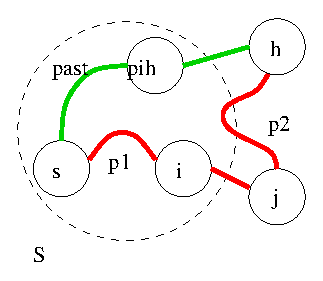
\includegraphics[width=5cm]{dijkstracorrect}
\end{center}
\caption{The crux of the argument in Dijkstra's correctness theorem
  \ref{thm:dijkstra}.}
\label{f:dijkstrathm}
\end{figure}

\subsection{A more refined implementation}
In the complexity analysis of the simple implementation of Dijkstra's
algorithm,\index{algorithm!Dijkstra} we did not exploit the fact that
$V$ is implemented as a priority queu\index{queue!priority} (see
Sect.~\ref{s:search:heap:priorityq}). Moreover, because only reached
nodes\index{node!reached} can be settled,\index{settled} $V$ need only
contain unsettled, reached nodes\index{node!unsettled} at any
time. Because Step \ref{minimum} requires the node $v$ with minimum
$d_v$, we use $d_v$ as priorities. This, however, raises an issue:
since $d_v$ is updated every time an arc is
relaxed,\index{arc!relaxed} priorities might need to be changed for
nodes that are already in the queue. One way to implement the update
of the priority\index{priority} $d_v$ for the node $v$ in a
heap\index{heap} (the tree structure that implements a priority queue,
see Sect.~\ref{s:search:heap}) is to delete $v$ ($O(\log n)$) and
re-insert it with the updated priority ($O(\log n)$).

\subsubsection{Pseudocode}
In the pseudocode, we distinguish between $V$, the set of nodes, and
$Q$, the priority queue\index{queue!priority} of reached unsettled
nodes.\index{node!reached}\index{node!unsettled}
\begin{algorithmic}[1]
\STATE $\forall v\in V\; d_v=\infty$, $d_s=0$;
\STATE $\forall v\in V\; \mbox{\sf p}_v=s$;
\STATE $Q.\mbox{\tt insert}(s,d_s)$;
\WHILE{$Q\not=\varnothing$}
  \STATE Let $u=Q.\mbox{\tt popMin}()$; \label{Qminimum}
  \FOR{$(u,v)\in\delta^+(u)$} \label{Qreach}
    \STATE Let $\Delta=d_u+c_{uv}$; 
    \IF{$\Delta < d_v$} \label{Qrelax}
      \STATE Let $d_v = \Delta$;
      \STATE Let $\mbox{\sf p}_v = u$;
      \STATE $Q.\mbox{\tt delete}(v)$; {\tt // no effect if $v\not\in
        Q$} \label{Qupdpriority1} 
      \STATE $Q.\mbox{\tt insert}(v,d_v)$; \label{Qupdpriority2}
    \ENDIF
  \ENDFOR
\ENDWHILE
\end{algorithmic}

\subsubsection{Complexity}
By Exercise \ref{ex:settleonce}, nodes are settled exactly once. This
implies that Step \ref{Qminimum} is executed $O(n)$ times, each taking
$O(\log n)$; and also that each arc is relaxed\index{arc!relaxed}
exactly once, since its head vertex must be settled in order for an
arc to be relaxed inside the loop at Step \ref{Qreach}; since priority
update takes $O(\log n)$, as remarked above, this implementation is
$O((n+m)\log n)$ overall. This is worse than $O(n^2)$ if the digraph
is dense\index{digraph!dense} but better if it is sufficiently
sparse,\index{sparse} which is most usually the case.

There exists also an $O(m+n\log n)$ Dijkstra
algorithm\index{algorithm!Dijkstra} implementation using more refined
data structures.

\subsection{The point-to-point SPP}
Solving the point-to-point SPP\index{P2PSPP} from $s$ to $t$ can be
seen as a ``part'' of the SPP: it suffices to stop the search as soon
as $t$ is settled, since, by definition, a settled node will keep its
priority until the end of the algorithm.

Accordingly, we can use a Dijkstra's
algorithm\index{algorithm!Dijkstra} modified by inserting the code
below between Step \ref{Qminimum} and \ref{Qreach}:
\begin{algorithmic}
\IF{$u=t$}
  \STATE exit;
\ENDIF
\end{algorithmic}

\section{Floyd-Warshall algorithm}
The Floyd-Warshall algorithm\index{algorithm!Floyd-Warshall} finds all
shortest paths\index{path!shortest} (i.e.~it solves the
ASP)\index{ASP} on a digraph\index{digraph} $G=(V,A)$ with any arc
weight function\index{function!arc!weigth} $c:A\to\mathbb{R}$.

\subsection{Data structures}
As data structures, we use two $n\times n$ matrices $p,d$: $p_{uv}$ is
the predecessor\index{predecessor} of $v$ in the shortest path from
$u$; $d_{uv}$ is the cost of the shortest path from $u$ to $v$. The
principle of the algorithm is the following: for each node $z$ and
node pair\index{node!pair} $u,v$, we check whether the current
shortest path from $u$ to $v$ can be improved by passing through $z$.
\begin{center}
\psfrag{u}{$u$}
\psfrag{v}{$v$}
\psfrag{z}{$z$}
\psfrag{puv}{$\mbox{\sf p}_{uv}$}
\psfrag{pzv}{$\mbox{\sf p}_{zv}$}
\includegraphics[width=6cm]{FW}
\end{center}
If so, we update $d_{uv}$ to $d_{uz}+d_{zv}$ and $p_{uv}$ to
$p_{zv}$, otherwise we consider the next triplet $z,u,v$.

\subsection{Pseudocode}
I find this algorithm is the very simplest to remember!
\begin{algorithmic}[1]
\STATE $\forall u,v\in
V\;d_{uv}=\left\{\begin{array}{rl}c_{uv}&\mbox{if }(u,v)\in
A\\ \infty & \mbox{otherwise} \end{array}\right.$
\STATE $\forall u,v\in V\;\mbox{\sf p}_{uv}=u$ 
\FOR{$z\in V$}
  \FOR{$u\in V$}
    \FOR{$v\in V$}
      \STATE $\Delta=d_{uz}+d_{zv}$; \label{FWupdate}
      \IF{$\Delta<d_{uv}$}
         \STATE $d_{uv} = \Delta$; 
         \STATE $\mbox{\sf p}_{uv} = \mbox{\sf p}_{zv}$; 
      \ENDIF
    \ENDFOR
  \ENDFOR
\ENDFOR
\end{algorithmic}

The complexity of the Floyd-Warshall algorithm is clearly $O(n^3)$.

\begin{ex}
Prove that the algorithm is correct. Try to express the following
concept formally: {\it at termination, every possible triplet was
  checked}.
\end{ex}

\subsection{Negative cycles}
\label{s:path:negcycle}
It is interesting to remark that the Floyd-Warshall algorithm can also
solve the NCP.\index{NCP} Assume there is a negative cycle through
$u$; when $u=v$, the ``triangulations'' through other nodes $z$ will
eventually yield $d_{uu}<0$, since a path from $u$ to itself via the
negative cycle will have negative weight. Whenever that happens,
terminate the algorithm: a negative cycle was found.

The modification to the pseudocode above is trivial: after Step
\ref{FWupdate}, insert this code:
\begin{algorithmic}
\IF{$\Delta<0$}
  \STATE exit;
\ENDIF
\end{algorithmic}


%% %%%%%%%%%%%%%%%%%%%%%%%%%%%%%%%%%%%%%%%%%%%%%%%
%% %%%%%%%%%%%%%%%%% PART IV %%%%%%%%%%%%%%%%%%%%
%% %%%%%%%%%%%%%%%%%%%%%%%%%%%%%%%%%%%%%%%%%%%%%%%

%% \part{A graph class implementation}

%% %%%%%%%%%%%%%%%%% CHAPTER: GRAPH IMPLEMENTATION %%%%%%%%%%%%%%%%%%%%
%% \chapter{Graph implementation}
%% \label{c:graphimpl}
%% In Ch.~\ref{c:graph} we gave the basic definitions of
%% graphs\index{graph} and subgraphs.\index{subgraph} In this chapter,
%% with the help of some linear data structures\index{data
%%   structure!linear} introduced in Ch.~\ref{c:linear}, we shall put
%% graph-related notions in practice, and implement a graph class in
%% Java.\index{Java}

%% \section{Software architecture}
%% Our implementation consists of three files:
%% \begin{itemize}
%% \item {\tt graphTest.java}, which contains the single class {\tt
%%   graphTest}, which in turn only contains the the (static) {\tt
%%   main}\index{main} function;
%% \item {\tt graph.java}, which contains the single class {\tt graph},
%%   which in turn contains two different data representations of the
%%   graph,\index{graph!representation} and a set of methods for acting
%%   on the graph data;
%% \item {\tt arc.java}, which contains the single class: {\tt arc}, which
%%   describes the data structure for storing an
%%   arc\index{graph!arc}\index{arc}.
%% \end{itemize}
%% This gives rise to the very simple software architecture shown in
%% Fig.~\ref{fig:graphswarch}.
%% \begin{figure}[!ht]
%% \begin{center}
%% \includegraphics[width=11cm]{grapharc}
%% \end{center}
%% \caption{The graph software architecture. The arrows show the
%%   occurrence of objects into class definitions.}
%% \label{fig:graphswarch}
%% \end{figure}

%% \section{The executable file}

%% \subsection{Compilation}
%% Compilation of the graph software system is launched by typing 
%% \begin{verbatim}
%% javac graphTest.java
%% \end{verbatim}
%% at the command prompt. This will produce three class files, one per
%% source file. The {\tt graphTest.class} file contains the point of
%% entry\index{point of entry} of the program. 

%% \subsection{Usage}
%% The syntax of {\tt graphTest} is as follows. The command
%% \begin{verbatim}
%% java graphTest
%% \end{verbatim}
%% yields some help. The syntax is 
%% \begin{verbatim}
%% java graphtest file cmd arguments
%% \end{verbatim}
%% where {\tt file} is a graph\index{graph} description in .gph format
%% (see below), {\tt cmd} is one of the commands below, and {\tt
%%   arguments}\index{argument} are optional arguments\index{argument} to
%% command {\tt cmd}. Argument {\tt cmd} can be any of the following
%% commands.\index{command}
%% \begin{itemize}
%% \item {\tt print}: print\index{print} the graph on screen (adjacency
%%   list\index{adjacency list}\index{list!adjacency} representation and
%%   arc list\index{arc list} representation);
%% \item {\tt graphviz}: output the graph in {\tt .dot} format (output
%%   file named {\tt graph-}$xyz${\tt .dot}), ready to be compiled into a
%%   drawing by the GraphViz\index{GraphViz} software
%% \item {\tt complement}: output the graph and its
%%   complement\index{graph!complement}\index{complement} in {\tt .dot}
%%   format (only implemented for undirected
%%   graphs)\index{graph!undirected}
%% \item {\tt linegraph}: output the graph and the corresponding line
%%   graph\index{graph!line}\index{line graph} in {\tt .dot} format (only
%%   implemented for undirected graphs)
%% \item {\tt contract [vertexlist]}: output the graph and the
%%   minor\index{graph!minor}\index{minor} obtained by
%%   contracting\index{contraction} the subgraph\index{subgraph} induced
%%   by the vertices in {\tt vertexlist} (a space-separated list of vertex
%%   indices) in {\tt .dot} format (only implemented for undirected
%%   graphs)
%% \item {\tt induced [vertexlist]}: output the graph and the subgraph
%%   induced by the vertices in {\tt vertexlist} (a space-separated list
%%   of vertex indices) in {\tt .dot} format (only implemented for
%%   undirected graphs)
%% \item {\tt maximalstable}: print a maximal stable
%%   set\index{set!stable}\index{stable} in the graph
%% \item {\tt vertexcolor}: print a vertex
%%   coloring\index{coloring}\index{vertex!coloring} for the graph. 
%% \end{itemize}

%% \section{The {\tt arc} class}
%% The {\tt arc} class implements a an unweighted
%% arc.\index{arc!unweighted} It assumes that the set $V$ of vertices of
%% the graph is enumerated by integers, i.e.~$V=\{1,\ldots,n\}$. In
%% practice, vertices are represented by {\tt Integer}s:\index{{\tt
%%     Integer}} much the same as {\tt int}s, aside from a technical
%% difference, i.e.~an {\tt int} is an elementary data type\index{data
%%   type!elementary} (passed to functions by value),\index{value!passing
%%   by}\index{passing!by value}; an {\tt Integer} is a non-elementary
%% data type (passed to functions by reference).\index{reference!passing
%%   by}\index{passing!by reference}

%% Here is the class declaration.\index{class!declaration}
%% \begin{verbatim}
%% public class arc {
%%     // maximum allowed number of vertices
%%     public static Integer maxVcard = 1000000; 
%%     public Integer source;
%%     public Integer dest;
%%     public boolean directed;

%%     // constructor
%%     public arc(Integer s, Integer d, Boolean dir);

%%     // print
%%     public void print();

%%     // override the equals method for HashMap to work
%%     // notice directed is not compared: in other words, an arc (u,v)
%%     // is equal to the edge {u,v}
%%     public boolean equals(Object o);
%%     // override the hashCode method for HashMap to work
%%     public int hashCode();
%% }
%% \end{verbatim}
%% An object of this class encodes the arc $(\mbox{\tt source},\mbox{\tt
%%   dest})$ or the edge\index{edge} $\{\mbox{\tt source},\mbox{\tt
%%   dest}\}$, according to whether {\tt directed} is assigned value {\tt
%%   true} or {\tt false}. It has a constructor,\index{constructor} a
%% print\index{print} method, and two technical methods which define the
%% behaviour of {\tt arc} objects when stored in a {\tt
%%   HashMap}.\index{{\tt HashMap}}

%% \section{The {\tt graph} class}

%% \section{The {\tt graphTest} class}



%%% end 

\bibliographystyle{plain} \bibliography{pcc}

%%%%%%%%%%%%%%%%%%%%%%%%%%%%%%%%%%%%%%%%%%%%%%%%%%%%%%%%%%%%%%%%%%%%
% name:         data_structures.tex
% author:	    Leo Liberti
% purpose:      book for INF421
% history:      120604 - work started (over the Atlantic, south of 
%                        Iceland)
%%%%%%%%%%%%%%%%%%%%%%%%%%%%%%%%%%%%%%%%%%%%%%%%%%%%%%%%%%%%%%%%%%%%%
\documentclass[a4paper]{book}

\usepackage{amsmath}
\usepackage{amsfonts}
\usepackage{amssymb}         %additional math symbols
\usepackage{amsopn}
\usepackage{theorem}          %additional LaTeX2e package 
\usepackage{latexsym}
\usepackage{mathrsfs}		%calligraphic fonts
\usepackage{tikz}
\usepackage{pgfplots}
%\usepackage{tkz-arith}
\usepackage{tikz-qtree}
\usepackage{tkz-graph}
%\usepackage{tkz-berge}
\usepackage{url}
\usepackage{verbatim}
\usepackage{algorithm}
\usepackage{algorithmic}
\usepackage[Lenny]{fncychap}
\usepackage{graphicx}        %graphic and .eps files
\usepackage{psfrag}
\usepackage{hyperref}

\input{../../../templates/definecolors.tex}

\setlength{\parindent}{0.5cm}
\setlength{\parskip}{0.3cm}
% the following settings leave nearly no margins. For defaults, rem out.
\setlength{\oddsidemargin}{0.5cm}
% rem out following for one-side only
\setlength{\evensidemargin}{-0.58cm}
%%
\setlength{\textwidth}{16cm}
\setlength{\textheight}{23cm}
\setlength{\footskip}{1cm}
\setlength{\topmargin}{0cm}

%% ______________________etc_____________________________
\makeindex
\pagestyle{headings}
\renewcommand{\baselinestretch}{1}
% N.B. if paper has sections and subsections add "[section]"
%      or "[subsection]" at the end of the following 5 lines.
\newtheorem{result}{\ }[section]
\theoremstyle{changebreak}                % (see LATEX2E\THEOREM.DTX)
\newtheorem{thm}[result]{Theorem}
\newtheorem{defn}[result]{Definition}
\newtheorem{lem}[result]{Lemma}
\newtheorem{cor}[result]{Corollary}
\newtheorem{prop}[result]{Proposition}
\newtheorem{eg}[result]{Example}
\newtheorem{ex}[result]{Exercise}
\newenvironment{proof}
 {{\sl Proof.}\hspace*{1 ex}}%
 {{\nopagebreak\hspace*{\fill}$\Box$\par\vspace{12pt}}}
%
\renewcommand{\vec}[1]{\underline{#1}}
\newcommand{\transpose}[1]{{#1}^{\top}}
\DeclareMathOperator{\dom}{\mathrm{dom}}
\DeclareMathOperator{\inc}{\mathrm{inc}}
%

\setcounter{secnumdepth}{6}
\setcounter{tocdepth}{4}

\begin{document}

\thispagestyle{empty}

\begin{center}
{\LARGE INF421: Data Structures and algorithms} \\ [4cm]
{\sc \Large Leo Liberti} \\ [1cm]
{\it LIX, Ecole Polytechnique, 91128 Palaiseau, France} \\ [1cm]
\url{liberti@lix.polytechnique.fr} \\ [4cm]
\today
\end{center}

\newpage

\thispagestyle{empty}
\vspace*{5cm}
\begin{flushright}
{\it To\footnote{Not a spelling mistake.} Much}
\end{flushright}

\newpage

\thispagestyle{empty}

Chers \'el\`eves,

vous avez entre vos mains la premi\`ere version de mon polycopi\'e
pour le cours INF421 ({\it Les bases de l'algorithmique et de la
programmation}) de l'Ecole Polytechnique. En tant que premi\`ere
version, ce polycopi\'e contiendra sans doute beaucoup d'erreurs:
merci de m'envoyer un email \`a \url{leoliberti@gmail.com} pour m'en
faire part, si vous en trouvez. 

Je vous rappelle que le website du cours INF421 
\begin{center}
\url{www.enseignement.polytechnique.fr/informatique/INF421/}
\end{center}
contient beaucoup de mat\'eriel didactique. Le blog
\begin{center}
\url{inf421.wordpress.com}
\end{center}
contient du mat\'eriel didactique suppl\'ementaire quand le cours est
actif. Pour le reste de l'ann\'ee, j'y publie n'importe quoi. 

%% L'ann\'ee derni\`ere, j'ai re\c{c}u des critiques de la part des
%% \'el\`eves principalement sur trois points: (i) la disconnexion entre
%% ce qui \'etait enseign\'e en amphi et les exercices des TDs; (ii)
%% l'absence du code dans les {\it slides} present\'es pendant le cours;
%% (iii) l'absence du polycopi\'e. Evidemment, ce texte est une r\'eponse
%% au point (iii). Pour ce qui concerne le point (ii), ce polycopi\'e
%% contient beaucoup de code dans les premiers chapitres, qui
%% dispara\^{\i}t au fur et \`a mesure que le discours passe du codage
%% \`a l'abstraction du m\^eme (l'algorithme), jusqu'\`a en avoir presque
%% plus dans les derniers chapitres. En tout cas, on n'apprend pas a
%% coder en lisant du code: il faut le cr\'eer avec son propre cervau,
%% et le b\^atir avec ses propres mains.

%% Pour ce qui concerne le point (i), voici mon opinion. Assister \`a une
%% s\'eance d'amphi qui introduise exactement ce qui sera vu dans le TD,
%% sert a un seul but: minimiser le travail de l'\'el\`eve, en maximisant
%% ses r\'esultats. Je comprends donc bien les critiques en ce sens, mais
%% les \'el\`eves sont partie en cause: c'est {\it evident} que vous
%% vouliez le maximum des r\'esultats avec le minimum de
%% l'effort. Malheureusement, cet approche minimise aussi le
%% d\'eveloppement de l'intelligence. Il produirait un cours le plus
%% modulaire possible, avec chaque argument, reduit \`a ses termes
%% minimales, pr\^et \`a \^etre m\'emoris\'e ou compris avec le moins
%% possible de fatigue mentale, et pas d'autres notions enseign\'ees sauf
%% celles qui seraient directement utiles pour l'exercice du TD. Sachez
%% donc que {\it intelligence} et un mot qui vient du latin {\it
%%   interligo}, un m\'elange de ``entre'' ({\it inter}) et ``associer''
%% ({\it ligare}).  L'intelligence, \`a la base, c'est faire des liens
%% entre des conceptes diff\'erentes. L'acteur intelligent, si ce
%% n'\'etait pas encore clair, c'est la personne qui {\it \'etablit} les
%% liens. Si l'enseignant vous donne tous les liens, ou, pire, vous les
%% coupes pour ``modulariser'' les arguments, emp\`eche le
%% d\'eveloppement de votre intelligence. Aucun enseignant ferait \c{c}a
%% expr\`es: il lui serait moralement interdit. Sans compter que le but
%% de ce cours d'informatique n'est pas du tout celui de ``faire bien les
%% exercices en TD'': les exercices sont un {\it moyen}, pas un {\it
%%   fin}.

%% Comme c'est un enseignant (moi) qui a \'ecrit ce polycopi\'e, et pas
%% un \'el\`eve, il va de soi que c'est {\it mes} souhaits qu'il
%% refl\`ete, et pas le v\^otres. Ce texte vous propose bien plus
%% d'arguments du minimum essentiel, ne vous encapsule pas trop les
%% savoirs, et fait tr\`es peu d'efforts pour vous faciliter la vie en
%% TD. Il y a \'evidemment des forts liens conceptuels entre polycopi\'e,
%% amphis, et TDs; mais il y a des notions dans le cours qui ne sont
%% mentionn\'ees qu'en TD, qu'en amphi, que dans ce polycopi\'e.  C'est
%% cens\'e am\'eliorer l'esprit d'ind\'ependence de l'\'el\`eve, ainsi
%% que sa cr\'eativit\'e. En somme, ce texte, mes amphis, les TDs, et
%% l'entiert\'e de mon travail d'enseignant, vont dans la direction de
%% vous contraindre a {\it faire des efforts pour comprendre}. Votre
%% affiliation prestigieuse d\'eclare \`a la France enti\`ere que vous
%% \^etes les ingenieurs les plus intelligents et plus capables: pensez a
%% devenir plus intelligents, et laissez tomber la minimisation des
%% efforts.

%% Par ailleurs, je vous invite a m'envoyer des emails, m\^eme beaucoup
%% d'emails, si vous avez des questions, pr\'ecises ou non, sur le
%% contenu du cours: d\'evelopper l'intelligence se fait par lecture, par
%% \'ecoute, par apprentissage pratique, mais encore plus par
%% discussion. Un livre peut vous dire ce qui est, mais les questions les
%% plus ardues concernent ce qui n'est pas: quand vous trouvez une
%% incoh\'erence entre ce que vous avez compris et ce que vous lisez
%% quelque part, aucun livre peut vous r\'epondre, car ce doute ne
%% concerne que vous. C'est bien dans des cas pareils que vous devez
%% demander l'aide de vos enseignants. Jusqu'\`a ce que je resterai votre
%% enseignant, je vous promets de faire de mon mieux pour vous repondre,
%% sinon dans la foul\'ee, dans journ\'ee; ou, au pire, dans la semaine.

\begin{flushright}
{\sc Leo Liberti}, Paris, Ao\^ut 2012
\end{flushright}



\tableofcontents

\nocite{mehlhorn,baptiste_inf421,dowek,knuthNew1}

%%%%%%%%%%%%%%%%%%%%%%%%%%%%%%%%%%%%%%%%%%%%%
%%%%%%%%%%%%%%%%% PART I %%%%%%%%%%%%%%%%%%%%
%%%%%%%%%%%%%%%%%%%%%%%%%%%%%%%%%%%%%%%%%%%%%

\part{Preliminaries and reminders}

%%%%%%%%%%%%%%%%% CHAPTER: INTRODUCTION %%%%%%%%%%%%%%%%%%%%

\chapter{Computation}
\label{c:computation}

\begin{center}
\fbox{\begin{minipage}{13cm}{\small {\sc Abstract}. What
        is a computer and how we represent it formally: what can be
        computed and what cannot. Programming languages: what can be
        expressed and what cannot. Touching on Java. Efficient
        computation: problems, data structures, and
        algorithms. Worst-case complexity.}
\end{minipage}}
\end{center}

This introductory chapter briefly touches on some deep theoretical
topics, most of which are presented in the INF423 course, as well as
in many textbooks (e.g.~\cite{minsky}).

\section{Computer hardware}
\label{s:computation:practice}
A computer is a piece of machinery engineered for carrying out
computations electronically. Most computers consist of a {\it Central
  Processing Unit} (CPU),\index{CPU} some banks of {\it Random-Access
  Memory} (RAM)\index{RAM}, several {\it Input/Output} (IO)\index{IO}
devices, that allow the communication with the user and the external
world, as well as a motherboard that wires all the components
together. At any given instant, the CPU has a {\it state}\index{state}
$s$ out of a possible set $S$ of states. With a given frequency $f$,
the CPU reads and executes a new {\it instruction},\index{instruction}
supplied by the user, which changes its state. According to the state
it is in, the CPU may perform arithmetic or logical operations on
data, read data from or write it to RAM, send data to or receive it
from IO devices.

\subsection{Programs}
\label{s:computation:programs}
Instructions are normally supplied by the user as an ordered list,
also called a {\it program}.\index{program} The ``default behaviour''
of the CPU is to execute instructions in the user-provided sequence,
unless the instruction itself explicitly tells the CPU to jump to a
given point in the sequence. There are instructions that tell the CPU
to test a given logical condition and act differently according to the
results of the test.

We remark that, since a program is defined as an ordered list of
instructions, and any sublist of a list is also a list, any
``subprogram'' is also a program, i.e.~we might use the same term
``program'' to refer to certain subsets of instructions of a given
program.

\section{Computer model}
\label{s:computation:theory}
The computer, as described in Sect.~\ref{s:computation:practice}, was
first conceived by Alan Turing\index{Turing, A.} in 1936 \cite{turing}.
Turing's mathematical model of the computer is called {\it Turing
  Machine} (TM).\index{Turing!machine} A TM\index{TM} consists of an
infinite tape,\index{tape} divided into a countably infinite number of
cells,\index{cell} with a device (called {\it head})\index{head} that
can read or write symbols\index{symbol} out of a given alphabet
$A$\index{alphabet} on each cell of the tape. According to the state
$s\in S$ the TM is in, the head either reads, or writes, or moves its
position along the tape. Any TM has a set of instructions that tell it
how to change its state. Turing showed that there exist TMs which can
simulate the behaviour of any other TM: such TMs are called {\it
  Universal Turing
  Machines}\index{Turing!machine!universal}
  \index{universal!Turing machine} (UTM).\index{UTM}

Turing's work spawned further research, from the 1950s onwards, aimed
at simplifying the description of UTMs, involving scientists of
the caliber of Shannon\index{Shannon} \cite{shannonUTM} and
Minsky\index{Minsky} \cite{minskyUTM}. More recently,
Rogozhin\index{Roghozin} \cite{roghozin} described UTMs with low
values of $(|S|,|A|)$, e.g. $(24,2)$, $(10,3)$, $(7,4)$, $(5,5)$,
$(4,6)$, $(3,10)$, $(2,18)$. It appears clear that there is a
trade-off\index{trade-off} between number of states and number of
symbols in the alphabet.

\subsection{Models of computation}
\label{s:computation:models}
UTMs are not the only existing models of computation\index{model of
  computation} --- several others exist, sometimes very different from
each other (see e.g.~the {\it Game of Life},\index{Game of Life} a
model for bacteria diffusion \cite{gameoflife}). Such models are said
to be Turing-complete\index{Turing-complete} if they can
simulate\index{simulation} a UTM. ``Simulating'', in this context,
means using a different model $C$ of computation in order to mimick
the behaviour of a UTM. To prove this, it suffices to show that every
instruction, state and symbol of the UTM can be simulated by $C$. If
the UTM can also simulate $C$, then $C$ is said to be
Turing-equivalent.\index{Turing-equivalent}

\subsection{Church's Thesis}
\label{s:computation:churchthesis}
{\it Church's Thesis}\index{Church, A.}\index{Church's thesis}
is the statement that every Turing-complete model of computation is
also Turing-equivalent. So far, no Turing-complete model of
computation was found to be more ``powerful'' than the UTM.

\section{Languages}
\label{s:computation:languages}
A {\it programming language}\index{language}\index{programming
  language} is a set of rules for formulating instructions of a
computer program.\index{program} A language, by itself, does not
compute. Programs written in a given language do not compute
either. The relevant model of computation is a computer running a
program written in a given language. It makes sense, however, to
question the ``expression power'' of a language, e.g.~is it
sufficiently expressive that it can write a program that, executed on
a computer, simulates a UTM? If so, then the language is called {\it
  universal}.\index{universal!language} It was shown in
\cite{universallang} that, in order to be universal, a given language
should be able to express concatenation, tests and loops.

The {\it concatenation}\index{concatenation} of two instructions $I_1$
and $I_2$ is the program $I_1; I_2$. By induction, the concatenation
of two programs $P_1$ and $P_2$ is the program $P_1; P_2$. A {\it
  test}\index{test} instruction modifies the sequence of the
instructions in a program according to whether a given logical
condition is true or false. A {\it loop}\index{loop} is an instruction
that tells the CPU to repeat the execution of a given program.

It is important to keep in mind the distinction between the language
and its underlying computing model. A computing model with no
provision for simulating a memory\index{memory} device (be it a
tape\index{tape} or RAM\index{RAM} or otherwise), may very well
execute a program written in a universal language, but the resulting
computing model will fail to be
Turing-complete.\index{Turing-complete}

\subsection{Declarative languages}
\label{s:computation:declarative}
So far, we made the assumption that programs consist of instructions
that tell a computer (be it hardware or theoretical) to act in certain
ways. The class of languages for expressing such programs are called
{\it imperative
  languages}.\index{language!imperative}\index{imperative} There is
another class of programming languages, called {\it declarative
  languages},\index{language!declarative}\index{declarative} which are
designed to describe sets (e.g., the set of even numbers can be
described as $\{n\in\mathbb{N}\;|\;n\bmod 2 = 0\}$). Java,\index{Java}
C,\index{C} C++,\index{C++} Basic,\index{Basic}
Fortran,\index{Fortran} Pascal\index{Pascal} are all imperative
languages.

Insofar as a computer acts on input data to produce output data, it
can be seen as a function. Since the formal definition of a
function\index{function} $f$ is a set $F$ of pairs $(\iota,\omega)$
such that $f(\iota)=\omega$, we can describe a function by means of
the set $F$. In this sense, in order to fully describe $f$, it would
suffice to list a set of mathematical conditions that hold for any set
$V$ if and only if $V=F$. Declarative\index{declarative} programming
languages allow such descriptions. Prolog,\index{Prolog}
LISP,\index{LISP} CAML,\index{CAML} AMPL\index{AMPL} are all
declarative languages (most also integrate some imperative
instructions, too). An interesting example of a declarative universal
language\index{language!universal} is given by Diophantine
equations,\index{Diophantine equation}
i.e.~polynomial\index{polynomial} equations with integer coefficients,
where the solutions are constrained to be integers \cite{jones}: the
solution set of certain Diophantine equations define functions that
turn out to describe the input/output pairs of a UTM.\index{UTM}

\subsection{Decidability}
\label{s:computation:decidability}
Functions $\mathbb{N}\to\mathbb{N}$ represented by TMs are called {\it
  computable}.\index{function!computable}\index{computable} Sets
$V\subseteq\mathbb{N}$ that are domains\index{domain} (or
co-domains)\index{co-domain} of computable functions are called {\it
  recursively enumerable}\index{recursively enumerable}. If $V$ and
$\mathbb{N}\smallsetminus V$ are both recursively enumerable, then
they are both also called {\it
  recursive}\index{set!recursive}\index{recursive} or {\it
  decidable}\index{set!decidable}\index{decidable}.  Given a set
$V\subseteq\mathbb{N}$ and an integer $v\in\mathbb{N}$, one may ask
whether $v\in V$ or not. This is a fundamental decision
problem\index{problem!decision}\index{decision} in number theory. It
turns out that $V$ is recursively enumerable if and only if there is a
program that answers YES when $v\in V$, but may answer wrongly or even
fail to terminate when $v\not\in V$; moreover, $V$ is decidable if and
only if there is a program that answers YES when $v\in V$ and NO when
$v\not\in V$. This provides a further link between imperative and
declarative languages.

It should appear clear that recursively enumerable sets are of limited
value as far as proving that an answer to a problem is correct: if the
algorithm answers YES, it may be a true positive or a false negative,
and there is no way to tell. Moreover, how is a user supposed to know
whether a program fails to terminate\index{termination!failure} or is
simply taking a long time?  Accordingly, we try to frame problems so
that the solution set is decidable.\index{decidable}

On the other hand, several interesting sets fail to be decidable.
Take, for example, Hilbert's\index{Hilbert, D.} tenth problem: {\it
  determine whether or not there exists a mechanical procedure for
  solving a given Diophantine equation}.\index{Diophantine equation}
Given the extent of work on Diophantine equations carried out ever
since Greek civilization, this is certainly an interesting problem.
It remained open until Matyasevi\v{c}\index{Matyasevi\v{c}} answered
in the negative \cite{jones}, by proving that there are parametric
Diophantine equations whose solution set spans the totality of
recursively enumerable\index{recursively enumerable} sets. Since
decidable\index{decidable} sets are a proper subset of recursively
enumerable sets, there clearly are Diophantine equations whose
solution set is undecidable.\index{undecidable}

\subsection{Java}
\label{s:computation:java}
Our programming language of choice is Java\footnote{Its basic syntax
  was provided in previous courses, such as INF311 and
  INF321.}.\index{Java} In Java, one can:
\begin{itemize}
\item initialize a variable:\index{variable}
\begin{verbatim}
  int i;
\end{verbatim}
\item assign a constant value to a variable:\index{constant}
\begin{verbatim}
  i = 3;
\end{verbatim}
\item define a function:\index{function}
\begin{verbatim}
  int f(int s) {
    s = 1;
    return s;
  }
\end{verbatim}
e.g.~the above defines the trivial function $f:\mathbb{N}\to\{1\}$
that maps every integer to 1
\item test a condition:\index{test}
\begin{verbatim}
  if (i < 3) {
    f(i);
  } else {
    i = 0;
  }
\end{verbatim}
\item loop indefinitely over a program:\index{loop}
\begin{verbatim}
  while(true) {
    f(i);
  }
\end{verbatim}
\end{itemize}
The fundamental constructs above can be mixed in a number of
syntactically correct ways in order to produce increasingly complex
programs.

\section{Efficiency}
\label{s:computation:efficiency}
Although the questions ``what can you compute with a given computer?''
and ``what can you write with a given language?'' are certainly the
most fundamental --- and universality\index{universal} gives a
theoretical measure of how far computers and languages can provide an
answer to these questions --- there remains the important question of
efficiency.\index{efficient} How efficiently can a language express a
certain program, and how fast can a computer execute a given program?
The answers to these questions largely define the science (and art) of
algorithmics.

\subsection{Structuring data}
\label{s:computation:datastructures}
In the vast majority of real computers, RAM\index{RAM} is organized as
a long but finite list of {\it Binary digITs} (bits).\index{bit} In
the jargon of TMs, the underlying alphabet\index{alphabet} is
$\{0,1\}$, and each cell of the tape can hold either
symbol.\index{symbol} Although this is sufficient to guarantee
universality, it is cumbersome for people to program using only two
symbols.

Accordingly, a {\it data structure}\index{data!structure} is a
segmentation of memory\index{memory} that carries a certain meaning to
the user. For example, people noticed that most integers arising in
practice are in the range $\mbox{\tt
  int}=\{-2^{31},\ldots,2^{31}-1\}$.\index{int@{\tt int}} Integers in this
range can be described by sequences of exactly 32 bits (i.e.~4
bytes\footnote{One byte contains 8 bits.}: 31 bits are used to store
the absolute value, and the remaining bit is used for the sign). In TM
jargon, this is akin to taking 32 binary cells on the tape\index{tape}
and declaring them to simply be ``one cell'' which can hold any
integer in the range {\tt int}.  This, by the way, also provides a
very simple example of simulation\index{simulation} of a TM with
$|A|=32$ by a TM with $|A|=2$.

In real computers, we are not bound to segmenting memory using only
one data structure:\index{data!structure} a part of memory can hold
{\tt int}s, another can hold bits, and yet another can hold {\tt
  double}s\index{double@{\tt double}} (a data structure for storing a certain
subset of rational numbers). Moreover, most programming languages
allow users to declare their own data structures by combining the
elementary\index{data!structure!elementary} ones in different ways. In
order to make it even easier to write programs with user-defined data
structures,\index{data!structure!user-defined}
languages\label{language} usually also allow for pairing such
structures with dedicated user-defined
functions\index{function!user-defined} that handle them appropriately.

In Java, user-defined data structures are called {\it
  objects};\index{object} the formal description of an object in terms
of elementary data structures is a {\it class}.\index{class} The data
items occurring in classes are called {\it
  attributes},\index{attribute} and the functions items are called
{\it methods}.\index{method}

\subsection{Problems}
\label{s:computation:problem}
It should be clear that programs take data as input, manipulate these
data, and produce data as output. Not all possible data are valid for
input (think of a program that takes a 16-bit integer as input and is
fed a 32-bit one instead --- something like this made the Ariane 5
rocket explode!), and the set of output data is well-defined. A
program $P$ therefore defines a set ${\cal I}$ of possible inputs and
a set ${\cal O}$ of possible outputs. Do ${\cal I},{\cal O}$ uniquely
define the program that produced them? The answer is no: take for
example ${\cal I}={\cal O}=\{n\in\mbox{\tt int}\;|\;n\bmod 2=0\land
n\in[0,10]\}$. This can be obtained with either of the following
(different) programs:
\begin{verbatim}
  /* code 1 */
  int i = 0;
  while(i < 10) {
    i += 2;
    System.out.println(i);
  }

  /* code 2 */
  int i = 0;
  while(i < 10) {
    if (i % 2 == 0) then
      System.out.println(j);
    }
    i++;
  }
\end{verbatim}

We formally define a {\it problem}\index{problem} to be a set of pairs
$(\iota,\omega)$. A problem is {\it
  decidable}\index{problem!decidable}\index{decidable} if there is at
least a program (or TM) $P$ with input set ${\cal I}$ and output set
${\cal O}$ such that $\omega=P(\iota)$ for all $(\iota,\omega)\in
{\cal I}\times {\cal O}$. A decidable problem can also be seen as the class
of all programs that produce the same output $\omega\in {\cal O}$ on a
given input $\iota\in {\cal I}$, and reject all input not in ${\cal
  I}$.

\subsection{Algorithms}
\label{s:computation:algorithm}
Loosely speaking, we use ``algorithm'' and ``program''
interchangeably; a ``program'' usually indicates actual code that can
be compiled and executed by a computer, whereas an ``algorithm'' is an
idealized model of a program. An algorithm might contain a statements
in natural (rather than formal, see Sect.~\ref{s:tree:language})
language, or be written formally but for a machine that does not exist
in practice. In general, ``algorithm'' has a theoretical connotation,
whereas ``program'' has a practical one. More formally, an {\it
  algorithm}\index{algorithm} is any program solving a decidable
problem.\index{problem!decidable}

\subsubsection{Algorithmic complexity}
\label{s:computation:complexity}
As mentioned in \ref{s:computation:problem}, several
algorithms\index{algorithm} may solve the same problem.\index{problem}
This immediately raises an important question: {\it which one should
  we use?} In the clearest-cut case, there might be an algorithm which
takes less time and memory: it might be difficult to find it, but the
question has a well-defined answer. In most cases, there is a
trade-off\index{trade-off} between time and space: some algorithms may
take less time but more memory, and vice versa. We refer to time
measures as {\it time complexity}\index{complexity!time} and {\it
  space complexity}.\index{complexity!space} Since RAM is generally
less costly than time, apart from a special cases time complexity is
used more often than space complexity. In the sequel, we almost always
mention complexity to mean ``time complexity''.

As programs consist of sequences of basic instructions, each of which
takes (almost) the same time to execute on the CPU, time complexity
evaluations usually count the number of instructions to be executed
before the program terminates. Space complexity evaluations count the
number of bytes of RAM that the program allocates whilst running. These
questions are, unfortunately, ill-defined: programs may behave well
with a given input and badly with another. Accordingly, we consider
three possibilities: {\it worst-case
  complexity},\index{complexity!worst-case} {\it best-case
  complexity},\index{complexity!best-case} and {\it average-case
  complexity}.\index{complexity!average-case}

Best-case complexity is not often used: an algorithm may be very fast
on short or trivial input, but this says nothing about how the
algorithm will perform in general. Worst-case complexity is more
informative (as it gives a guarantee --- if an algorithm is fast in
the worst case, all the better for the general case!) and usually not
too difficult to evaluate: this is why it is the most studied
case. Average-case complexity is very informative, as it aims at the
general case, but it is often difficult to compute. And unless we can
also compute the variance attached to the average, it might be
misleading.

Below, we shall therefore mostly concentrate on worst-case time
complexity.

\subsubsection{Worst-case time complexity calculations}
\label{s:computation:timeworstcase}
We let $P$ be a program, and $t_P$ be the number of instructions that
are executed in $P$. Notice that, because of tests and loops, this is
different from the number of instructions actually written in the
program. The following rules-of-thumb hold.
\begin{itemize}
\item Basic assignments,\index{assignment} arithmetic/logical
  operations and tests all have $t_P=1$.
\item If $P,Q$ are programs and $P;Q$ is their
  concatenation,\index{concatenation} then
\begin{equation}
  t_{P;Q} = t_P+t_Q. \label{eq:concatenation}
\end{equation}
\item If $T$ is a logical test\index{test} and $P,Q$ are programs, then
\begin{equation}
  t_{\mbox{\scriptsize\tt if($T$)$P$\,else\,$Q$}} = t_T +
  \max(t_P,t_Q).\label{eq:test}
\end{equation}
Notice that the use of the $\max$ operator implements the
worst-case\index{complexity!worst-case} policy; average- and best-case
would yield different formul{\ae}.
\end{itemize}
The case of the loop\index{loop} is more complicated, as it depends on
whether the body of the loop is independent on the
termination\index{termination} condition or not. Consider the
following algorithm $P$, where $Q$ is a program.
\begin{verbatim}
  int i = 0;
  while (i < n) {
    Q();
    i = i + 1;
  }
\end{verbatim}
In this algorithm, $\mbox{\tt Q()}$ does not depend on $\mbox{\tt i}$,
and therefore we have $t_P = t_{\mbox{\scriptsize\tt i=0}} +
n(t_Q+t_{\mbox{\scriptsize\tt i$<$n}}+t_{\mbox{\scriptsize\tt i+1}}+
t_{\mbox{\scriptsize\tt i=$\cdot$}})+t_{\mbox{\scriptsize\tt
    i$<$n}}=2+n(t_Q+3)$. The last test term refers to the test
$\mbox{\tt i}<\mbox{\tt n}$ when {\tt i} and {\tt n} have the same
value, which fails and allows the loop to terminate.

\subsubsection{Complexity orders}
\label{s:computation:complexityorder}
Suppose we are able to determine that $t_Q=\frac{1}{2}n$. Then
$t_P=\frac{1}{2}n^2+3n+1$. Since we would like to know the behaviour
of this algorithm in the worst-case,\index{complexity!worst-case} it
is interesting to look at the asymptotic behaviour of $t_P(n)$ for
$n\to\infty$. It is clear that the dominating term is
$\frac{1}{2}n^2$; moreover, asymptotically, the $\frac{1}{2}$
constant\index{constant} is not so important. We simply say that $t_P$
asymptotically behaves like $n^2$, and write it as $t_P\in O(n^2)$, or
``$t_P$ is $O(n^2)$''.\index{$O(\cdot)$}

In general, we say that a function\index{function} $f(n)$ is {\it
  order\index{complexity!order} of $g(n)$} (and write it ``$f(n)$ is
$O(g(n))$'') if:
\begin{equation}
  \exists c > 0 \quad \exists n_0\in\mathbb{N} \quad \forall n>n_0
    \quad (f(n) \le c\, g(n)).
\end{equation}
In words: there are positive real $c$ and integer $n_0$ such that
$c\,g(n)$ dominates $f(n)$ for all $n>n_0$. Table \ref{tab:orders}
lists some complexity orders for various functions of $n$.
\begin{table}[!ht]
\begin{center}
\begin{tabular}{|l|l|} \hline
{\it Functions} & {\it Order} \\ \hline
$an+b$ with $a,b$ constants & $O(n)$ \\
polynomial of degree $d'$ in $n$ & $O(n^d)$ with $d\ge d'$ \\
$n+\log n$ & $O(n)$ \\ 
$n+\sqrt{n}$ & $O(n)$ \\
$\log n+\sqrt{n}$ & $O(\sqrt{n})$ \\
$n\log n^3$ & $O(n\log n)$ \\ 
$\frac{an+b}{cn+d}$, $a,b,c,d$ constants & $O(1)$ \\
\hline
\end{tabular}
\end{center}
\caption{Complexity orders of some functions of $n$.}
\label{tab:orders}
\end{table}
Evidently, an effort should be made to find the lowest possible
worst-case order, i.e.~although the function $2n+1$ is certainly
$O(n^4)$, it is much more informative to say that it is $O(n)$.

We remark that if $t_P(n)$ is a constant\index{constant} (i.e.~$n$
does not appear in the expression for $t_P$), then it is $O(1)$;
e.g.~looping $10^{100}$ times over an $O(1)$ program is itself $O(1)$.

%%%%%%%%%%%%%%%%%%%%%%%%%% CHAPTER: JAVA BASICS %%%%%%%%%%%%%%%%%%%%%%%%
%%%%%

\chapter{Java basics}
\label{c:java}

\begin{center}
\fbox{\begin{minipage}{13cm}{\small {\sc Abstract}.  Short
      introduction to Java. Variables, Objects, Classes, Interfaces,
      and Data types. Functions, values and references. An example:
      plotting the graph of a mathematical function on the screen. }
\end{minipage}}
\end{center}


Each computer brand --- or even model --- is different. CPU\index{CPU}
design and capabilities evolve in time, as does the set of
instructions\index{instruction} they can understand. On the other
hand, programmers spend a long time learning a programming
language,\index{language!programming} and once they are proficient in
one, they are unwilling to spend more time learning others. Thus,
languages should not change even though the underlying computer that
executes them will. This is attained in essentially two ways:
\begin{itemize}
\item updating the compiler\index{compiler} or
  interpreter;\index{interpreter}
\item simulating a ``software computer'' that does not change.
\end{itemize}
The first paradigm is by far the most common. Since the instructions
that a CPU can actually execute are very different from the constructs
of human-employed programming languages, these must be translated into
executable code in order to be run. {\it Compilers}\index{compiler} or
{\it interpreters}\index{interpreter} are used for this task. A
compiler translates a user program at once, and writes a file
containing executable code. An interpreter translates the instructions
of a user program one after the other, following the program flow, and
executes each one immediately. Compiled languages are: C,\index{C}
C++,\index{C++} Pascal,\index{Pascal}, Fortran\index{Fortran},
(relatively) recent Basic\index{Basic} dialects, and many
others. Interpreted languages are: perl,\index{perl}
python,\index{python} early Basic dialects, and many
others. Typically, compiled languages yield code that is faster to
execute than interpreted languages; on the other hand, changing an
interpreted program is easier than changing a compiled one.

Java,\index{Java} on the other hand, rests on a piece of software that
simulates a virtual computer: in Java terms, this is a {\it Virtual
  Machine} (VM).\index{virtual machine} The virtual machine can evolve
in time to take advantage of technical progress in computer design,
but always offers the same set of primitives to the programs it can
execute. This also makes it easy to port Java applications to
different platforms (e.g.~Windows,\index{Windows}
MacOSX,\index{MacOSX} Linux):\index{Linux} it suffices to implement an
appropriate VM.

\section{Development of a Java program}
\label{s:java:example}
A Java program is encoded in an ASCII\index{ASCII} text file ---
better use the first 128 characters and steer clear of accents. Open
your favourite text editor and type:
\begin{verbatim}
/*
  Name: helloWorld.java
  Purpose: a "hello world" program in Java
  Author: Leo Liberti (from an idea by B. Kernighan)
  Source: Java
  History: 17/10/2011 work started
*/

class helloWorld {
    public static void main( String [ ] args ) {
        System.out.println("hello world");
    }
}
\end{verbatim}
Save as {\tt helloWorld.java}. Now open a terminal window, and type:
\begin{verbatim}
javac helloWorld.java
java helloWorld
\end{verbatim}
The first command calls the Java compiler,\index{javac@{\tt
    javac}}\index{java@{\tt java}} which translates the text above into
code that can be executed on the Java VM. The second command tells the
Java VM to execute this code. As an effect of the execution, the
computer should print {\tt hello world} on the same terminal as the
commands were issued.

\subsection{Variables}
\label{s:java:variables}
In Java, variable symbols\index{variable!symbol} can store
values\index{variable!value} or addresses.\index{variable!address}
Typically, variables having elementary data
types\index{data!type!elementary} such as {\tt boolean}, {\tt
  int},\index{int@{\tt int}} {\tt long},\index{long@{\tt long}} {\tt
  float},\index{float@{\tt float}} {\tt double},\index{double@{\tt double}} {\tt
  char}\index{char@{\tt char}} store values: if {\tt int a} is a variable,
then its value is stored at a certain address in
memory.\index{memory!address} If {\tt myClass} is a user-defined
class,\index{class!user-defined} then the variable {\tt myClass C} has
a non-elementary data type:\index{data!type} in this case, Java stores
in {\tt C} a memory address, which points to a part of memory which
contains the actual value of {\tt C}.

\subsubsection{References}
Variables containing addresses are also called {\it
  references}.\index{reference} Users need not concern themselves
excessively with storage implementation details, aside for a few (but
important) occurrences to do with copying data from a non-elementary
data typed variable to another. Will Java copy the addresses or the
values themselves? Copying addresses is known as {\it shallow
  copy},\index{copy!shallow} whilst copying values is known as {\it
  deep copy}.\index{copy!deep}

Consider a reference {\tt a} whose value is an address $a$ of a memory
cell containing the value $b$. This is represented graphically as
shown below.
\begin{center}
\begin{tikzpicture}
  [memory/.style={rectangle,draw=black!50,fill=blue!20}]
  \node at (0,0.5) [memory] (reference) {$a$};
  \node at (0,0) {{\tt a}};
  \node at (2,0.5) [memory] (address) {$b$};
  \node at (2,0) {$a$};
  \draw [->] (reference.east) -- (address.west);
\end{tikzpicture}
\end{center}

\subsection{Comments}
\label{s:java:comments}
A {\it comment}\index{comment} is simply text inserted in a program so
as to remind human readers of the meaning of the surrounding
instructions. Natural,\index{language!natural} rather than formal
languages,\index{language!formal} are usually employed. Comments are
supposed to make code clearer and easier to understand. A program with
no comments will probably be unreadable; on the other hand, users will
most likely ignore comments if every single line is commented.

In Java, comments can be single line or multi-line. A double slash
(``{\tt //}'') means that the rest of the line, until its end, will
contain a comment. A multi-line comment starts with ``{\tt /*}'' and
ends with ``{\tt */}''. An example of a multi-line comment is given in
the {\tt helloWorld} program.

Comments are ignored by the Java compiler,\index{compiler} but some
relevant information can be stored in comments, to be read by an
appropriate {\it preprocessor}\index{preprocessor} --- this is
software that interprets the program according to different rules, and
is usually called prior to (or independently of) the compiler. This
can be useful to automatically produce documentation for a given
software, for example.

\subsection{Classes}
A {\it class}\index{class} is the Java\index{Java} equivalent of a
mathematical set\index{set} defined by a property
$P$,\index{set!property} i.e.~$\{x\;|\;P(x)\}$. In Java, the property
$P$ is a description of the {\it data type}\index{data!type} of each
piece of data $x$ in the class, e.g.~$x$ might store an integer, a
float and a string.

In Java, every program must contain at least a class. A {\it
  class}\index{class} is the formal Java definition of a data
structure.\index{data!structure} It usually contains a list of
variable names\index{variable!name} (with associated data
type)\index{data!type} and a list of functions that determine how the
values stored in the variables change. The class in the {\tt
  helloWorld}\index{helloWorld@{\tt helloWorld}} program, called {\tt
  helloWorld}, only contains one function called {\tt
  main}.\index{main@{\tt main}}

A class is an entity which resides in the Java program. Once compiled
and executed, a class, strictly speaking, does nothing. The Java
VM,\index{virtual machine} however, may create (either by default or
because instructed to do so) {\it objects}\index{object} of any given
class. An object is therefore an instance of the class stored in
memory. If we draw a parallel between Java and mathematical language,
a class is to a set what an object is to an element. In other words, a
class is a description of the data structure, whereas an object is an
actual piece of data that is structured in memory according to the
specification of its class. For example, the class
\begin{verbatim}
class IntPair {
  int first;
  int second;
}
\end{verbatim}
defines a data structure\index{data!structure} that holds two integers
between $-2^{31}$ and $2^{31}-1$. An object {\tt myIntPair} of this
class, defined as:
\begin{verbatim}
  IntPair myIntPair = new IntPair;
\end{verbatim}
holds a pair of integers in memory. The name {\tt myIntPair} is
arbitrary --- the fact that it is similar to the class name is only
supposed to help a reader identify the class directly from the object.
In general, two different objects of the same class hold different
data.

Class members,\index{class!member} be they data ({\it
  attributes})\index{attribute} or functions ({\it
  methods}),\index{method} can some specifiers, such as {\tt
  public},\index{public} {\tt static}\index{static} and others. Public
class members can be referenced from instructions\index{instruction}
outside the class. Static members are stored at a single
address\index{memory!address} in memory, which means that all objects
of the same class all share static data.\index{data!shared} By
default, members are neither public nor static, which means that they
can only be referenced from instructions inside the class, and each
object of the class can refer to its own private\index{private} copy
of the data.

\subsubsection{The {\tt this} attribute}
Suppose the class {\tt myClass} has a method {\tt myMethod}. Within
the {\tt myMethod} code, the Java keyword {\tt this}\index{this@{\tt this}}
is a reference to the object which will execute {\tt myMethod}. This
means that two objects of the same class have the same attribute {\tt
  this}, but this will hold two different memory addresses depending
on which object refers to it. 

\subsubsection{Inheritance}\index{inheritance}\index{class!inheritance}
Just as sets can, in mathematics, be subsets of other sets, classes
can be subclasses of other classes. A class\index{class} {\tt C}
describing each of its objects\index{object} as storing an integer, a
float and a string might well be a subclass of another class {\tt B}
whose objects only store an integer and a float.

Inheritance is useful for several reasons. For example, if we need
both {\tt B} and {\tt C} in our code and do not have inheritance, we
must write
\begin{verbatim}
  public class B {
    int i;
    float f;
  }

  public class C {
    int i;
    float f;
    String s;
  }
\end{verbatim}
Notice we are duplicating some code.\index{code!duplication} If we
need to change the {\tt float} to a {\tt double} later on, and still
require {\tt B} to be a subclass of {\tt C}, we must remember to
change the code in different places: since people forget such details,
it will very likely give rise to a bug.\index{bug} Notice that a
similar type of bug destroyed the Ariane\index{Ariane 5} 5 on its
maiden flight. Inheritance helps avoid this issue. We define
{\tt C} as follows:
\begin{verbatim}
  public class C extends B {
    String s;
  }
\end{verbatim}
In other words, we explicitly tell the compiler\index{compiler} that
there is a relationship between the two classes. This not only
shortens the code, but decreases the chances of coding mistakes by
delegating to the compiler the responsibility of checking that the
relationship $\mbox{\tt C}\subseteq\mbox{\tt B}$ is maintained
throughout the code.

\subsubsection{Interfaces}
\label{s:java:interface}
An {\it interface}\index{interface}\index{class!interface} is a very
special kind of class, whose purpose is that of enforcing
conformance\index{conformance} to a certain class
structure.\index{class!structure} For example, in a Graphical User
Interface (GUI)\index{GUI} every window (including full program
windows, dialog boxes and warning boxes) must conform to certain basic
notions about windows: e.g., they possess a width, a height, a title
and a frame, they have some standard buttons for minimizing,
maximizing and closing, they have some standard pull-down menu, and
they must remember their contents so that these can be re-drawn if
another window is temporarily dragged over it. A programmer who
designs a new type of window might be tempted to design a window of a
different kind, say with no standard buttons. However, all other
programs running on the GUI automatically assume that all windows have
standard buttons, so they are free to call the associated code: in the
long run, this might cause bugs and unforeseen behaviour. To avoid
this, the compiler itself enforces conformance with a standard idea of
window in the GUI by means of an interface: all classes defining a
window must inherit from the window interface, and implement its
functions as they see fit.

Remark that interfaces have no data and only contain the names,
argument types and return types of the member functions. No object can
be defined as member of an interface class
only.\index{object!interface} By contrast, objects of different
classes that both implement\index{interface!implementation} (i.e.,
inherit from) the same interface class can both be attributed the
interface data type. Let us consider the example of a normal window
and of a special type of window whose aspect ratio is always 3:2.
\begin{verbatim}
interface Window {
  int getWidth();
  int getHeight();
}

class MainWindow implements Window {
  int width;
  int height;
  public int getWidth() {
    return width;
  }
  public int getHeight() {
    return height;
  }
}

class FixedRatioWindow implements Window {
  int size;
  public int getWidth() {
    return 3*size;
  }
  public int getHeight() {
    return 2*size;
  }
}
\end{verbatim}
In subsequent code, we might wish to loop over all windows. This is
possible thanks to inheritance from the {\tt Window} array.
\begin{verbatim}
  MainWindow mw = new MainWindow();
  FixedRatioWindow frw = new FixedRatioWindow();
  ArrayList<Window> a;
  // ...
  a.add(mw);
  a.add(frw);
  // now we can loop over the elements of a
\end{verbatim}
Notice that {\tt ArrayList<Window>}\index{ArrayList@{\tt ArrayList}}
implements an array of interfaces (we shall discuss the funny angular
brackets later, see Sect.~\ref{s:linear:map:parametrized}).

\subsection{Functions}
In general, functions\index{Java!function} may take a list of
arguments\index{function!argument} of given type, implement an
algorithm\index{algorithm} with such arguments as input, and then
optionally return a value of given type to the calling function. For
example, the Java function {\tt f} taking an integer input and
returning its square is implemented as follows.
\begin{verbatim}
int f(int x) {
  return x*x;
}
\end{verbatim}

\subsubsection{Passing by reference or value} 
Consider the mathematical function $f(x)=x^2$, and the possible
C++\index{C++} implementation:
\begin{verbatim}
dataType f(dataType x) {
  x *= x;
  return x;
}
\end{verbatim}
(we remark this is a valid construct in Java too, but we refer to C++
here for technical reasons). The {\tt dataType} keyword is simply the
data type of the argument {\tt x} and of the return\index{return
  value} value of {\tt f}. It might describe an integer\index{integer}
or a floating-point\index{floating-point} number.

Now consider a calling function:
\begin{verbatim}
void g() {
  dataType x = 2;
  dataType y = f(x);
  cout << x << " + **2 = " << y << endl; // print string on screen
}
\end{verbatim}
and try and imagine what the printed output will be like. Obviously,
{\tt y} will take value 4. But what value will {\tt x} take? The
definition of {\tt f} changes the value of {\tt x}, but will this
change be remembered in the calling function?

The answer depends on whether {\tt f} has access to the value of {\tt
  x}, or to the address\index{address} where {\tt x} is stored in
memory.\index{memory} In the first case, this value will be stored by
{\tt f} in a new memory area: the {\tt x} in {\tt g} and the {\tt x}
in {\tt f} are stored in two distinct memory cells, whose values can
be changed independently. in the second case, if {\tt f} changes the
value of {\tt x}, {\tt g} will retrieve the changed value, because
{\tt x} in {\tt f} and {\tt x} in {\tt g} are stored at the same
memory address. In the first case, {\tt x} is {\it passed by
  value},\index{passing!by value}\index{value!passing by} and in the
second, {\tt x} is {\it passed by reference}\index{passing!by
  reference}.\index{reference!passing by}

In Java, passing by value or by reference is not a user choice.
Elementary data types\index{data!type!elementary} ({\tt boolean}, {\tt
  int}, {\tt long}, {\tt float}, {\tt double}, {\tt char}) are passed
by value, and all other data types (including user-defined classes)
are passed by reference.

\subsubsection{The {\tt main} function}
The function {\tt main}\index{main@{\tt main}} takes as argument an
array\index{array} called {\tt args},\index{args@{\tt args}} and
returns no data --- this is the meaning of the {\tt
  void}\index{void@{\tt void}} right before the function declaration.
In the case of the {\tt helloWorld} program, all it does is to print
out to the system screen the string ``hello world''.

\subsubsection{Specifiers}
Some details about how functions are translated to executable code by
the Java compiler\index{Java!compiler}\index{compiler} can be
influenced by code {\it specifiers}.\index{specifier}

The {\tt main} function of the {\tt helloWorld} program, for example,
is specified to be {\tt public} and {\tt static}. The first specifier,
{\tt public},\index{public} states that this function can be called
from other functions, even outside the class (normally, functions in a
class can only be called by other functions in the same class). The
second specifier, {\tt static},\index{static} tells the
compiler\index{compiler} that any object of the class {\tt helloWorld}
will share a single copy of the {\tt main}\index{main@{\tt main}} function:
the function code will be stored at a precise address in
memory,\index{memory!address} and this address will be stored in every
object\index{object} of the class {\tt helloWorld}. Functions and
variables that are declared {\tt static}\index{static} serve a purpose
of sharing data between different objects of the same class.

\subsection{Data types}
A class defines the type of data it encodes: if an object is a piece
of data, the class it belongs to is the {\it data
  type}.\index{data!type} In Java, we distinguish a small set of data
types, which includes {\tt boolean},\index{boolean@{\tt boolean}} {\tt
  int},\index{int@{\tt int}} {\tt long},\index{long@{\tt long}} {\tt
  float},\index{float@{\tt float}} {\tt double}\index{double@{\tt
    double}} and {\tt char}:\index{char@{\tt char}} these are called {\it
  elementary}.\index{data!type!elementary} Elementary data types do
not correspond to any defined class --- rather, these types are
hard-coded in the compiler.\index{compiler} This makes a difference as
far as functions are concerned. The instruction
\begin{verbatim}
void f(int a);
\end{verbatim}
will define a function called {\tt f} which takes as input an {\tt
  int} called {\tt a}. If the function {\tt f} changes the value
stored in {\tt a}, this has no effect on {\tt a} outside the function:
\begin{verbatim}
  int a = 2;
  f(a);
  System.out.println(a);
  // ...
  void f(int a) {
    a = 1;
  } 
\end{verbatim}

\subsection{The dot operator}
For Java instructions to refer to the
member\index{object!member}\index{member} {\tt first} of the object
{\tt myIntPair}, the dot\index{dot operator}\index{operator!dot}
operator is used, e.g.:
\begin{verbatim}
  myIntPair.first = 1;
\end{verbatim}
With this in mind, it is easy to interpret the instruction
\begin{verbatim}
  System.out.println("hello world");
\end{verbatim}
as a chain of embedded objects: it is a call to the function {\tt
  println}, which is in the object {\tt out},\index{System.out@{\tt System.out}}
which is itself one of the data in the object 
{\tt System}.\index{System@{\tt System}}

\subsection{The curly brackets}
In Java (and also in C\index{C} and C++),\index{C++} curly
brackets,\index{bracket!curly}\index{\{\}} (also known as
braces),\index{brace} are used to delimit the scope\index{scope} of a
set of instructions. Accordingly, they mark the beginning and end of a
class, function, but also of {\tt if} blocks\index{block!if}, and {\tt
  while}\index{block!while} and {\tt for}\index{block!for}
loops.\index{loop}

\subsection{The semicolon}
Every basic instruction\index{instruction!basic} in Java is terminated
by a semicolon.\index{;}\index{semicolon} Notice that a basic
instruction does not necessarily correspond to a line. Class or
function definitions are not considered basic instructions, insofar as
they are delimited by braces rather than ended by a semicolon.

\subsection{How code is executed}
A program can include several classes, defined in different
files.\index{file} However, for a program to yield executable
code,\index{code!executable} there must be a {\it point of
  entry},\index{point of entry} i.e.~a first function that the
Operating System\index{operating system} (OS)\index{OS} knows it can
call. This function can then call all the other functions in the
program. In Java, this first function is called {\tt main},\index{main@{\tt
    main}} it must be defined as {\tt static}\index{static} and {\tt
  void},\index{void} it takes as input the list of command line
arguments passed by the user to the program via the shell\index{shell}
prompt, and must be a {\tt public}\index{public} class
member.\index{class!member} Moreover, the name of the class containing
{\tt main} should have the same name as the Java file\index{file} it
is stored in (see the {\tt helloWorld} example).

\section{Arrays in Java}
\label{s:java:array}
An {\it array}\index{array} represents a list of objects\index{object}
of the same class. An example of an array of three {\tt int} having
value $2,1,-1$ is shown below.
\begin{center}
\fbox{2}\fbox{1}\fbox{-1}
\end{center}
The fact that the objects come one after the other is meant to suggest
that they are stored in memory at contiguous addresses. This may be
true or not, depending on the actual array implementation. It is
usually true to a degree: an array might well be implemented as a set
of distinct memory segments, each of which consists of contiguous
addresses. 

\subsection{Dimensions}
Arrays can be {\it linear}\index{array!linear} or {\it
  multidimensional}.\index{array!multidimensional} Mathematically
speaking, a linear array is similar to a vector,\index{vector} a
two-dimensional\index{array!two-dimensional} array to a
matrix,\index{matrix} and a multidimensional array to a
tensor.\index{tensor}

\subsection{The square bracket notation}
In Java, arrays are declared using square
brackets,\index{bracket!square} in one of the two ways below.
\begin{verbatim}
int[] myArray;
int myArray[];
\end{verbatim}
Declaring an array does not make it usable: first, we must allocate
some memory\index{memory!allocation} to it.
\begin{verbatim}
myArray = new int[4]; // reserves enough memory to hold 4 int
\end{verbatim}
It is common to combine the declaration and the memory allocation in
the same instruction (both alternatives will work).
\begin{verbatim}
int[] myArray = new int[4];
int myArray[] = new int[4];
\end{verbatim}
Multidimentional arrays get as many square bracket pairs as there are
dimensions.\index{dimension} The following defines a $(4\times 3\times
2)$ 3-dimensional array of {\tt int}.
\begin{verbatim}
int[][] x = new int[4][3][2];
\end{verbatim}
In Java, the number of components\index{component} in each dimension
need not be a constant. 
\begin{verbatim}
int n = 2;
int m = 3;
int[][][] x = new int[4][m][n];
\end{verbatim}


\section{Example: plotting the graph of a function}
In this section we shall present a simple worked-out Java example,
consisting entirely of static data, that plots\index{function!plot} a
function $y=f(x)$ of one variable on a text console\index{console}
screen. This program consists of a single class,\index{class} called
{\tt functionPlot},\index{functionPlot@{\tt functionPlot}} and resides
in a single file called {\tt functionPlot.java}. The class is declared
static\index{static} and contains a {\tt main}\index{main@{\tt main}}
function, as detailed above. The {\tt main} function performs the
following tasks:
\begin{enumerate}
\item initialize some data, such as the ranges $[x^L,x^U]$ where we
  wish to tabulate $f(x)$, the number $n$ of function table entries,
  as well as the size of the ``text screen'' (number of
  rows\index{row} and columns);\index{column}
\item compute two vectors:\index{vector} $(x_1,\ldots,x_n)$ such that
  $x_k\in[x^L,x^U]$ for all $k\le n$, and $(y_1,\ldots,y_n)$ such that
  $y_k=f(x_k)$ for all $k\le n$;
\item fill an integer\index{integer} array\index{array} {\tt screen}
  with zeroes, apart from those entries $(i,j)$ (set to 1) that best
  approximate the pairs $(x_k,y_k)$;
\item print the array {\tt screen} on the text console.\index{console}
\end{enumerate}

\subsection{A typical output}
\label{s:java:example:output}
A typical output with 20 rows, 75 columns, and
$f(x)=\frac{1}{4}x+\sin(x)$ in the range $[-10,10]$ is shown in
Fig.~\ref{f:fplot}.
\begin{figure}[!ht]
\begin{center}
\fbox{\begin{minipage}{13cm}
{ \small
  \verbatiminput{functionPlot.out}
}
\end{minipage}}
\end{center}
\caption{A typical output from {\tt functionPlot}.}
\label{f:fplot}
\end{figure}

\subsection{Comments and imports}
The {\tt filePlot.java} file starts with the usual
comments\index{comment} bearing some minimal information about the
program.
\begin{verbatim}
/*
  Name: functionPlot.java
  Purpose: plotting functions in ASCII
  Author: Leo Liberti
  Source: Java
  History: 120615 work started
*/
\end{verbatim}

Next, we {\it import}\index{import} some standard Java classes.
\begin{verbatim}
import java.io.*;
import java.util.*;
import java.lang.*;
\end{verbatim}
The {\tt import} command tells the compiler to read some other Java
code, which might include declarations\index{declaration} and
definitions\index{definition} of names occurring in the program. For
example, we shall make use of mathematical functions {\tt
  Math.sin}\index{sine} and {\tt Math.rint},\index{integer rounding}
as well as the print\index{print} functions {\tt
  System.out.print}\index{System.out@{\tt System.out}} and {\tt
  System.out.println}. We shall not explicitly declare these
functions, but rather instruct the compiler to look for them in some
standard libraries.\index{library!standard}

\subsection{The class declaration}
We present the class structure\index{class!structure} next. We remark
that the following class contains some function {\it
  declarations}\index{declaration} (specifiers, return type, name,
argument types) without the corresponding {\it
  definition}\index{definition} (the function code, contained in
braces);\index{brace} accordingly, the following code cannot be
compiled ``as is'': all function declarations need to be followed by
the corresponding definitions.  {\small
\begin{verbatim}
class functionPlot {
    //// Private data
    static int steps;    // number of function evaluations
    static double [] x;  // x coordinate values
    static double xL;    // lower bound for x coordinate values
    static double xU;    // upper bound for x coordinate values
    static double [] y;  // y coordinate values
    static double yL;    // lower bound for y coordinate values
    static double yU;    // upper bound for y coordinate values
    static int rows;     // number of text rows taken by plot
    static int columns;  // number of text columns taken by plot
    static int[][] screen;
    //// Public functions
    // this defines the function to be plotted
    public static double theFunction(double z);
    // initialize some values
    public static void initialize();
    // compute the x-y table
    public static void functionTable();
    // compute the minimum value of the y range
    public static double yMin();
    // compute the maximum value of the y range
    public static double yMax();
    // fill the screen array cells corresponding to x/y pairs with 1's
    public static void tableScreen();
    // loop over the screen array and either print a '*' (1) or a space (0)
    public static void printScreen();
    // this is the program's point of entry
    public static void main(String [] args);
}
\end{verbatim}
}

All the data in the {\tt functionPlot} class is declared {\tt
  static}. This implies that all data is shared\index{data!shared}
among all functions in the class. The first section of the class
declares a set of (private)\index{private} attributes\index{attribute}
which can only be accessed by functions within the class. There
follows a section containing the (public)\index{public} declarations
of all class functions.\index{class!function} Notice that the last
function {\tt main} is the point of entry\index{point of entry} of the
VM\index{virtual machine} when it executes the code. Every line is
commented for clarity.

\subsection{The {\tt main} function}
The {\tt main} function simply calls four other functions in order:
data initialization, function tabulation, filling of the {\tt screen}
array, and printing of the {\tt screen} array on the
console\index{console} screen.
\begin{verbatim}
    public static void main(String [] args) {
        initialize();
        functionTable();
        tableScreen();
        printScreen();
    }
\end{verbatim}

\subsection{Initialization}
The {\tt initialize} function simply assigns some
user-defined\index{user} constants to some parameter variables. Users
can change the behaviour of the program in certain ways by changing
these parameters, re-compiling and re-executing the program.
\begin{verbatim}
    public static void initialize() {
        // user: set values for steps, x range, rows/columns for plot
        steps = 150;   // 150 entries in function table
        xL = -10;      // lower bound for x range
        xU = 10;       // upper bound for x range
        columns = 75;  // number of columns on the console screen
        rows = 20;     // number of rows on the console screen
        // user: do not change anything beyond this point
        x = new double[steps];  // the x vector
        y = new double[steps];  // the y vector
    }
\end{verbatim}

\subsection{Function tabulation}
Tabulating a function $f$ of one variable means computing a set of
pairs $(x_k,y_k)$ such that $y_i=f(x_k)$, for $k\le n$ where
$n\in\mathbb{N}$ is given. Accordingly, we set up two linear
arrays\index{array!linear} {\tt x}, {\tt y} to hold {\tt steps} values
each.
\begin{verbatim}
    public static void functionTable() {
        double theStep = (xU - xL) / steps;
        x[0] = xL;
        for(int k = 1; k < steps; k++) {
            x[k] = x[k-1] + theStep;
            y[k] = theFunction(x[k]);
        }	
    }
\end{verbatim}
The function {\tt functionTable} calls another function, {\tt
  theFunction}, which is simply a user-changeable\index{user}
implementation of the mathematical function $f(x)$. For example, if
$f(x)=\frac{1}{4}x+\sin x$, we have
\begin{verbatim}
    public static double theFunction(double z) {
        // user: change the mathematical function here at leisure
        return 0.25*z + Math.sin(z); 
    }
\end{verbatim}
Notice here that we use the symbol {\tt z} instead of $x$ because we
already used a static variable\index{variable!static} {\tt x} to
denote the array\index{array} storing the first
components\index{components} of the function table pairs. Since {\tt
  x} is a static variable, every function in the class (including {\tt
  theFunction} can read it and change it. Had we used {\tt double x}
instead of {\tt double z} here, we would have {\it
  shadowed}\index{shadowing} the symbol {\tt x} that denotes the
array, rendering it inaccessible within this function. Also notice the
library function\index{library} {\tt sin}, which is a member function
of the class {\tt Math}.\index{Math@{\tt Math}}

\subsection{Converting the function table to an array}
We pave the way for printing\index{print} to the
console\index{console} screen. We model this screen by means of a
two-dimensional array\index{array!two-dimensional} {\tt screen},
indexed on rows\index{row} and columns.\index{column} Initially, we
fill {\tt screen} with zeroes. Later on, we loop\index{loop} over the
function table pairs, and we change {\tt screen}'s $(i,j)$-th entry to
a one whenever there is a pair $(x_k,y_k)$ such that $(i,j)$ is the
best integer approximation of $(x_k,y_k)$ (after appropriate
translation and scaling). More precisely, we let:
\begin{eqnarray*}
   j &=& \left\lfloor \frac{x_k-x^L}{x^U-x^L}\sigma +
   \frac{1}{2}\right\rfloor\\
   i &=& \left\lfloor \frac{y_k-y^L}{y^U-y^L}\rho +
   \frac{1}{2}\right\rfloor,
\end{eqnarray*}
where $\sigma$ is the number of columns ({\tt columns} in the code)
and $\rho$ the number of rows ({\tt rows} in the code. Adding
$\frac{1}{2}$ to a real number and taking its floor\index{floor} is
the same as rounding\index{integer rounding} it to the closest
integer.
\begin{verbatim}
    public static void tableScreen() {
        int i;
        int j;
        screen = new int [rows][columns];
        for(i = 0; i < rows; i++) {
            for(j = 0; j < columns; j++) {
                 screen[i][j] = 0;
            }
        }
        yL = yMin();
        yU = yMax();
        for(int k = 0; k < steps; k++) {
            j = (int) Math.rint(((x[k] - xL) / (xU - xL)) * columns);
            i = (int) Math.rint(((y[k] - yL) / (yU - yL)) * rows);
            if (i < rows && j < columns) {
                 screen[rows - (i + 1)][j] = 1;
            }
        }
    }
\end{verbatim}
The above function calls two other functions, {\tt yMin} and {\tt
  yMax}, that compute the minimum\index{minimum} and
maximum\index{maximum} of the $y$ range, and are defined as follows.
\begin{verbatim}
    public static double yMin() {
        double theMin = 1e30; // infinity
        for(int k = 0; k < steps; k++) {
            if (y[k] < theMin) {
                theMin = y[k];
            }
        }
        return theMin;
    }
    public static double yMax() {
        double theMax = -1e30; // -infinity
        for(int k = 0; k < steps; k++) {
            if (y[k] > theMax) {
                theMax = y[k];
            }
        }
        return theMax;
    }
\end{verbatim}

\subsection{Printing the screen}
We now come to the function that copies the arrays\index{array} {\tt
  screen} onto the console\index{console} screen. We interpret it so
that every time {\tt screen} contains a 1, a `{\tt *}' is printed on
the screen, while all zeroes are printed as spaces.
\begin{verbatim}
    public static void printScreen() {
        for(int i = 0; i < rows; i++) {
            for(int j = 0; j < columns; j++) {
                if (screen[i][j] == 1) {
                    System.out.print("*");
                } else {
                    System.out.print(" ");
                }
            }
            System.out.print("\n");
        }
    }
\end{verbatim}

\subsection{Compilation and running}
As for {\tt helloWorld}, the program {\tt functionPlot} can be
compiled and executed very simply as follows.
\begin{verbatim}
javac functionPlot.java
java functionPlot
\end{verbatim}
The output of {\tt functionPlot} with the user-defined\index{user}
parameters is given in Sect.~\ref{s:java:example:output}

\begin{ex}
Extend the {\tt functionPlot} class so that it also prints the $x$ and
$y$ axes.
\end{ex}

%%%%%%%%%%%%%%%%%%%%%%%%%%%%%%%%%%%%%%%%%%%%%%
%%%%%%%%%%%%%%%%% PART II %%%%%%%%%%%%%%%%%%%%
%%%%%%%%%%%%%%%%%%%%%%%%%%%%%%%%%%%%%%%%%%%%%%

\part{Data structures}

%%%%%%%%%%%%%%%%%%%%%%%%%% CHAPTER: GRAPHS %%%%%%%%%%%%%%%%%%%%%%%%%%%%%

%% TODO in this chapter: add some references

\chapter{Graphs}
\label{c:graph}

\begin{center}
\fbox{\begin{minipage}{13cm}{\small {\sc Abstract}.  
Directed and undirected graphs, neighbourhoods, complements, line
graphs, graph isomorphism. Subgraphs, stables and
cliques. Connectivity: paths and cycles. Basic operations on graphs.
}
\end{minipage}}
\end{center}

Data structures\index{data!structure} consist of pieces of data as
well as relations\index{relation} between and among them. We are going
to formalize this concept mathematically by means of
graphs.\index{graph} Graphs are also the appropriate mathematical
model for networks, be they transportation, communication, power,
social or other types of networks. Learning the ropes of graph theory
will therefore serve a double purpose.

\section{Directed graphs}
\label{s:graph:directed}
Formally, a {\it relation} on a set $V$ is a subset of the Cartesian
product\index{Cartesian product} $V\times V$ of all ordered pairs of
elements of $V$. Accordingly, we define a {\it directed
  graph}\index{graph!directed} (or {\it digraph})\index{digraph} as a
pair $G=(V,A)$ where $V$ is the set of {\it nodes}\index{node} (or
{\it vertices})\index{vertex} and $A$, a subset of $V\times V$, is
the set of {\it arcs}\index{arc} of the graph. Given a digraph $G$, we
sometimes denote its node set by $V(G)$ and arc set by $A(G)$. 
\begin{figure}[!ht]
\begin{center}
\begin{minipage}{3.5cm}
\begin{tikzpicture}
%\useasboundingbox (-1,-2) rectangle (8,2);
\SetVertexNormal
\SetGraphUnit{1}
\Vertex{1}
\EA(1){2}
\Edge[style={->}](1)(2)
\Loop[dist=1cm,dir=EA,style={->}](2)
\Loop[dist=1cm,dir=WE,style={->}](1)
\end{tikzpicture}
\end{minipage}
\begin{minipage}{3.5cm}
\begin{tikzpicture}
\GraphInit[vstyle=Normal]
\SetGraphUnit{1.1}
\tikzset{EdgeStyle/.append style={->}}
\Vertices{circle}{1,2,3,4,5}
\end{tikzpicture}
\end{minipage}
\begin{minipage}{3cm}
\begin{tikzpicture}
\GraphInit[vstyle=Normal]
\SetGraphUnit{1.3}
\tikzset{EdgeStyle/.append style={->}}
\Vertices[dir=\SO,x=0,y=0]{line}{1,2,3}
\Vertices[dir=\SO,x=1,y=0]{line}{4,5,6}
\Edge(1)(4)
\Edge(1)(5)
\Edge(2)(4)
\Edge(2)(6)
\Edge(3)(4)
\Edge(3)(5)
\end{tikzpicture}
\end{minipage}
\begin{minipage}{4cm}
\begin{tikzpicture}
\GraphInit[vstyle=Normal]
\SetGraphUnit{1}
\tikzset{EdgeStyle/.style={->,bend right}}
\Vertices{circle}{1,2,3}
\Loop[dist=1cm,dir=EA,style={->}](1)
\Loop[dist=1cm,dir=EA,style={->}](2)
\Loop[dist=1cm,dir=SOEA,style={->}](3)
\Edges(1,2,3,1)
\tikzset{EdgeStyle/.style={->}}
\Edges(1,3,2,1)
\tikzset{EdgeStyle/.style={->,bend right}}
\end{tikzpicture}
\end{minipage}
\end{center}
\caption{Examples of digraphs.}
\label{fig:digraphs}
\end{figure}
A reflexive relation pair $(v,v)$ is a special type of arc called a
{\it loop}\index{loop}, see e.g.~the loops $(1,1)$ and $(2,2)$ in the
leftmost graph of Fig.~\ref{fig:digraphs}. A {\it
  multidigraph}\index{multidigraph} associates a positive integer to
each arc called its {\it multiplicity}.\index{arc!multiplicity} An arc
with multiplicity higher than one is a {\it multiple
  arc}.\index{arc!multiple} A digraph is {\it
  simple}\index{digraph!simple} if it has no loops or multiple arcs.
A digraph is {\it empty}\index{digraph!empty} if its arc set is empty
(e.g.~second digraph from the left in Fig.~\ref{fig:digraphs}).  A
digraph is {\it bipartite}\index{bipartite}\index{digraph!bipartite}
if its node set $V$ can be partitioned in two sets $U,W$ such that
every arc $(u,w)\in A$ has $u\in U$ and $w\in W$ (e.g.~third digraph
from the left in Fig.~\ref{fig:digraphs}). A digraph is {\it
  complete}\index{digraph!complete}\index{complete} if its arc set is
$V\times V$ (e.g.~last digraph from the left in
Fig.~\ref{fig:digraphs}). Complete digraphs are also called {\it
  directed cliques}.\index{clique!directed}

\subsection{Directed neighbourhoods}
Given a digraph $G=(V,A)$ and a node $u\in V$, the node set
$N^+_G(u)=\{v\in V\;|\;(u,v)\in A\}$ is called the \textit{outgoing
  neighbourhood}\index{neighbourhood!outgoing} of $u$ with respect to
$G$. The node set $N^-_G(u)=\{v\in V\;|\;(v,u)\in A\}$ is called the
\textit{incoming neighbourhood}\index{star!neighbourhood} of $u$ with
respect to $G$ (see Fig.~\ref{fig:star}).
\begin{figure}[!ht]
\begin{center}
\psfrag{d-}{$N^-(7)$}
\psfrag{d+}{$N^+(7)$}
\includegraphics[width=5cm]{stars}
\end{center}
\caption{Incoming and outgoing neighbourhoods of node 7:
  $N^-(7)=\{1,2,3\}$ and $N^+(7)=\{4,5,6\}$.}
\label{fig:star}
\end{figure}
The \textit{outdegree}\index{outdegree} of a node $v\in V$ is the
cardinality of its outgoing neighbourhood, and similarly, the
\textit{indegree}\index{indegree} of $v\in V$ is the cardinality of
its incoming neighbourhood. In Fig~\ref{fig:star}, both the indegree
and the outdegree of node 7 are equal to 3. For $u\in V$, the arc set
$\delta^+_G(u)=\{(v,w)\in A\;|\;u=v\}$ is called {\it outgoing
  star}\index{star!outgoing} (or {\it outstar})\index{outstar} of $u$
with respect to $G$, and the arc set $\delta^-_G(u)=\{(w,v)\in
A\;|\;u=v\}$ is called {\it incoming star}\index{star!incoming} (or
{\it instar})\index{instar} of $u$ with respect to $G$. If there is no
ambiguity we dispense with the index $G$.

\section{Undirected graphs}
\label{s:graph:undirected}
Essentially, a graph is like a digraph where all arrows are replaced
by segments. More formally, a {\it graph}\index{graph} is a pair
$G=(V,E)$ where $V$ is a set of vertices and $E$ is a set of {\it
  edges}\index{edge} $\{u,v\}$ where $u,v\in V$. As for digraphs, for
a graph $G$ we sometimes denote by $V(G)$ its vertex set and by $E(G)$
its edge set. Whenever $u=v$ then $\{u,v\}=\{u\}=\{v\}$ is called a
loop. In {\it multigraphs},\index{multigraph} a positive integer
called multiplicity is assigned to each edge; edges with multiplicity
higher than one are called multiple (or parallel) edges (see
Fig.~\ref{fig:multigraph}). A graph without loops or multiple edges is
called {\it simple}.\index{graph!simple}
\begin{figure}[!ht]
\begin{center}
\begin{tikzpicture}[scale=1.3]
\SetGraphUnit{2}
\GraphInit[vstyle=Normal]
\tikzset{LabelStyle/.style= {draw,fill = yellow,text = red}}
\Vertex[L={$1$}]{A}
\EA[L={$2$}](A){B}
\tikzset{EdgeStyle/.append style = {bend left}}
\Edge(A)(B)
\tikzset{EdgeStyle/.append style = {bend right}}
\Edge(A)(B)
\end{tikzpicture}
\end{center}
\caption{A multigraph with two parallel edges.}
\label{fig:multigraph}
\end{figure}
Given a digraph, its \textit{underlying graph}\index{graph!underlying}
replaces every arc $(u,v)$ with the corresponding edge $\{u,v\}$ (see
Fig.~\ref{f:underlying}).
\begin{figure}[!ht]
\begin{center}
\begin{minipage}{5cm}
\begin{tikzpicture}[scale=1]
\GraphInit[vstyle=Normal]
\SetGraphUnit{1.1}
\tikzset{EdgeStyle/.append style={->}}
\Vertices{circle}{1,2,3,4}
\Edges(1,2,3,4,1)
\end{tikzpicture} 
\end{minipage}
\hspace*{1cm}
\begin{minipage}{5cm}
\begin{tikzpicture}[scale=1]
\GraphInit[vstyle=Normal]
\SetGraphUnit{1.1}
\Vertices{circle}{1,2,3,4}
\Edges(1,2,3,4,1)
\end{tikzpicture} 
\end{minipage}
\end{center}
\caption{A digraph and its underlying graph.}
\label{f:underlying}
\end{figure}
A graph is {\it empty}\index{graph!empty} if its edge set is empty. A
graph is {\it complete}\index{complete graph}\index{graph!complete}
(or a {\it clique})\index{clique} if every possible edge $\{u,v\}$ is
in $E$ for all $u\not=v\in V$. Notice that complete graphs are
simple. A graph $G=(V,E)$ is {\it
  bipartite}\index{bipartite}\index{graph!bipartite} if $V$ can be
partitioned in two sets $U,W$ such that every edge $\{u,w\}\in E$ has
$u\in U$ and $w\in W$.

\subsection{Complement graphs}
Given a graph $G=(V,E)$, consider the clique\index{clique} $K(V)$ on
$V$ with edge set\index{edge!set} $E_K$ consisting of all possible
vertex pairs.\index{vertex!pair} The graph $\bar{G}=(V,\bar{E})$,
where $\bar{E}=E_K\smallsetminus E$ is the {\it complement
  graph}\index{graph!complement} of $G$ (Fig.~\ref{f:complement}).
\begin{figure}[!ht]
\begin{center}
\begin{tikzpicture}[scale=1.3]
\node (v1) at (1,0) {\small $1$} ;
\node (v2) at (3,0) {\small $2$} ;
\node (v3) at (4,1) {\small $3$} ;
\node (v4) at (3,2) {\small $4$} ;
\node (v5) at (1,2) {\small $5$} ;
\node (v6) at (0,1) {\small $6$} ;
\node (v7) at (4.5,2.7) {\small $7$} ;
\draw (v1) to [thick] (v2) ;
\draw (v1) to [thick] (v3) ;
%\draw (v1) to [color=white] (v4) ;
\draw (v1) to [thick] (v5) ;
\draw (v1) to [thick] (v6) ;
%\draw (v1) to [color=white] (v7) ;
\draw (v2) to [thick] (v3) ;
%\draw (v2) to [color=white] (v4) ;
\draw (v2) to [thick] (v5) ;
%\draw (v2) to [color=white] (v6) ;
%\draw (v2) to [color=white] (v7) ;
\draw (v3) to [thick] (v4) ;
\draw (v3) to [thick] (v5) ;
%\draw (v3) to [color=white] (v6) ;
\draw (v3) to [thick] (v7) ;
%\draw (v4) to [color=white] (v5) ;
\draw (v4) to [thick] (v6) ;
\draw (v4) to [thick] (v7) ;
\draw (v5) to [thick] (v6) ;
\draw (v5) to [thick] (v7) ;
%\draw (v6) to [color=white] (v7) ;
\end{tikzpicture}
\hspace*{1cm}
\begin{tikzpicture}[scale=1.3]
\node (v1) at (1,0) {\small $1$} ;
\node (v2) at (3,0) {\small $2$} ;
\node (v3) at (4,1) {\small $3$} ;
\node (v4) at (3,2) {\small $4$} ;
\node (v5) at (1,2) {\small $5$} ;
\node (v6) at (0,1) {\small $6$} ;
\node (v7) at (4.5,2.7) {\small $7$} ;
%\draw (v1) to [color=white] (v2) ;
%\draw (v1) to [color=white](v3) ;
\draw (v1) to [thick] (v4) ;
%\draw (v1) to [color=white] (v5) ;
%\draw (v1) to [color=white] (v6) ;
\draw (v1) to [thick] (v7) ;
%\draw (v2) to [color=white] (v3) ;
\draw (v2) to [thick] (v4) ;
%\draw (v2) to [color=white] (v5) ;
\draw (v2) to [thick] (v6) ;
\draw (v2) to [thick] (v7) ;
%\draw (v3) to [color=white] (v4) ;
%\draw (v3) to [color=white] (v5) ;
\draw (v3) to [thick] (v6) ;
%\draw (v3) to [color=white] (v7) ;
\draw (v4) to [thick] (v5) ;
%\draw (v4) to [color=white] (v6) ;
%\draw (v4) to [color=white] (v7) ;
%\draw (v5) to [color=white] (v6) ;
%\draw (v5) to [color=white] (v7) ;
\draw (v6) to [thick] (v7) ;
\end{tikzpicture}
\end{center}
\caption{A graph and its complement.}
\label{f:complement}
\end{figure}

\begin{ex}
Propose an $O(n+m)$ algorithm for constructing the complement graph of a given
graph.
\label{ex:complement}
\end{ex}

\subsection{Neighbourhoods}
Given a graph $G=(V,E)$ and a vertex $v\in V$, we let $N_G(v)=\{u\in
V\;|\;\{u,v\}\in E\}$ be the {\it neighbourhood}\index{neighbourhood}
of $v$ and $\delta_G(v)=\{\{u,w\}\in E\;|\;u=v\}$ be the {\it
  star}\index{star} of $v$ in $G$. If there is no ambiguity, we
dispense with the index $G$.

\subsection{Graph isomorphism}
Two graphs $G=(V,E)$ and $G'=(V,E')$ on the same vertex
set\index{vertex!set} $V$ are {\it
  isomorphic}\index{graph!isomorphism} if there is a
bijection\index{bijection} $\pi:V\to V$ (also called an {\it
  automorphism}\index{automorphism} on $V$) such that:
\begin{equation*}
 \forall \{u,v\}\in E \ (\{\pi(u),\pi(v)\}\in E').
\end{equation*}
In other words, changing the vertex labels\index{vertex!label} does
not change the graph structure (see
Fig.~\ref{f:graphisom}).\index{graph!structure} Since $V$ is taken to
be finite, $\pi$ is also a permutation of $V$ (see
Sect.~\ref{s:recursion:permutation}).
\begin{figure}[!ht]
\begin{center}
\begin{tikzpicture}[scale=0.8]
\node (v1) at (1,0) {\scriptsize $1$} ;
\node (v2) at (3,0) {\scriptsize $2$} ;
\node (v3) at (4,1) {\scriptsize $3$} ;
\node (v4) at (3,2) {\scriptsize $4$} ;
\node (v5) at (1,2) {\scriptsize $5$} ;
\node (v6) at (0,1) {\scriptsize $6$} ;
\node (v7) at (4.5,2.7) {\scriptsize $7$} ;
\draw (v1) to (v2) ;
\draw (v1) to (v3) ;
\draw (v1) to (v5) ;
\draw (v1) to (v6) ;
\draw (v2) to (v3) ;
\draw (v2) to (v5) ;
\draw (v3) to (v4) ;
\draw (v3) to (v5) ;
\draw (v3) to (v7) ;
\draw (v4) to (v6) ;
\draw (v4) to (v7) ;
\draw (v5) to (v6) ;
\draw (v6) to [bend left=40] (v7) ;
\end{tikzpicture}
$\stackrel{\scriptsize \pi=(1\to 2\to 3\to 4\to 5\to 6\to 7\to 1)}{\longrightarrow}$
\begin{tikzpicture}[scale=0.8]
\node (v1) at (1,0) {\scriptsize $2$} ;
\node (v2) at (3,0) {\scriptsize $3$} ;
\node (v3) at (4,1) {\scriptsize $4$} ;
\node (v4) at (3,2) {\scriptsize $5$} ;
\node (v5) at (1,2) {\scriptsize $6$} ;
\node (v6) at (0,1) {\scriptsize $7$} ;
\node (v7) at (4.5,2.7) {\scriptsize $1$} ;
\draw (v1) to (v2) ;
\draw (v1) to (v3) ;
\draw (v1) to (v5) ;
\draw (v1) to (v6) ;
\draw (v2) to (v3) ;
\draw (v2) to (v5) ;
\draw (v3) to (v4) ;
\draw (v3) to (v5) ;
\draw (v3) to (v7) ;
\draw (v4) to (v6) ;
\draw (v4) to (v7) ;
\draw (v5) to (v6) ;
\draw (v6) to [bend left=40] (v7) ;
\end{tikzpicture}
\end{center}
\caption{The left graph is isomorphic to the right graph.}
\label{f:graphisom}
\end{figure}
We denote the application of $\pi$ to $G$ by $\pi G$. If $\pi G=G$,
then $\pi$ is an {\it graph
  automorphism}\index{graph!automorphism}\index{automorphism!graph} of
$G$. 

\begin{ex}
Verify that $\pi=(1\to 2\to 3\to 4\to 5\to 6\to 7\to 1)$ is not an
automorphism on the graph on the left of Fig.~\ref{f:graphisom}.
\end{ex}
The set of all graph automorphisms of a graph $G$ forms a {\it
  group}\index{group} with respect to the composition of bijections.
\begin{ex}
Verify that both $(1\to 5)$ is a graph automorphism of the graph on
the left of Fig.~\ref{f:graphisom}. Show that this graph has four
automorphisms (including the identity,\index{identity} which fixes
every $v\in V$), and, if you know what it means, that the structure of
its group\index{group!structure} is $C_2\times C_2$.
\end{ex}

\subsection{Line graph}
Given a graph $G=(V,E)$ where $E=\{e_1,\ldots,e_m\}$, the {\it line
  graph}\index{line graph}\index{graph!line} of $G$ is the graph
\begin{equation*}
   L(G) = (E,\{\{e_i,e_j\}\;|\;e_i\cap e_j\not=\varnothing\})
\end{equation*}
where each edge of $G$ is a vertex in $L(G)$, and edges of $L(G)$ are
pairs of edges of $G$ incident to the same vertex (see
Fig.~\ref{f:linegraph}).

\begin{figure}[!ht]
\begin{center}
\includegraphics[width=6cm]{linegraph}
\end{center}
\caption{A graph $G$ and its line graph $L(G)$ (thick lines).}
\label{f:linegraph}
\end{figure}

\begin{ex}
Prove that the degree $|N_{L(G)}(e)|$ of a vertex $e=\{u,v\}$ of
$L(G)$ is $|N_G(u)|+|N_G(v)|-2$.
\end{ex}

\begin{ex}
Give an algorithm for constructing $L(G)$ given $G$.
\end{ex}

\section{Subgraphs}
\label{s:graph:subgraph}
Given a graph (or digraph) $G=(V,E)$, a {\it subgraph}\index{subgraph}
is a graph $H=(U,F)$ such that $U\subseteq V$ and $F\subseteq E$. A
subgraph $H$ is {\it induced}\index{subgraph!induced} if, for all
$u,v\in U$ such that $\{u,v\}\in E$, we have $\{u,v\}\in F$ as well
(see Fig.~\ref{f:subgraph}).
\begin{figure}[!ht]
\begin{center}
\begin{minipage}{4cm}
\begin{tikzpicture}
\GraphInit[vstyle=Normal]
\SetGraphUnit{1.1}
\Vertices{circle}{1,2,3,4}
\Edge(1)(2)
\Edge(1)(3)
\Edge(1)(4)
\Edge(2)(3)
\Edge(3)(4)
\end{tikzpicture}
\end{minipage}
\hspace*{0.5cm}
\begin{minipage}{4cm}
\begin{tikzpicture}
\GraphInit[vstyle=Normal]
\SetGraphUnit{1.1}
\Vertex{1}
\NOWE(1){2}
\SOWE(2){3}
\Edge(1)(2)
\Edge(1)(3)
\end{tikzpicture}
\end{minipage}
\hspace*{0.5cm}
\begin{minipage}{4cm}
\begin{tikzpicture}
\GraphInit[vstyle=Normal]
\SetGraphUnit{1.1}
\Vertex{1}
\NOWE(1){2}
\SOWE(2){3}
\Edge(1)(2)
\Edge(1)(3)
\Edge(2)(3)
\end{tikzpicture}
\end{minipage}
\end{center}
\caption{A graph, a (non-induced) subgraph and an induced subgraph.}
\label{f:subgraph}
\end{figure}
If $G=(V,E)$ is a given graph (or digraph) and $U\subseteq V$, we
denote by $E[U]$ the subset of edges induced\index{induced} by $U$,
i.e.~the set of all edges in $E$ between vertices in $U$. Thus, if
$H=(U,F)$ is an induced subgraph of $G$, we can also denote $F$ by
$E[U]$. This notation is also extended to the whole subgraph: $H$ can
be denoted by $G[U]$.

\subsection{Stable and clique subgraphs}
\label{s:graph:subgraph:stable}
An induced subgraph\index{subgraph!induced} $H=(U,F)$ of $G$ is a
clique\index{clique} if it is complete,\index{complete} and a {\it
  stable}\index{stable} if it its edge set\index{edge!set} is
empty\index{empty} (see Fig.~\ref{f:cliquestab}).
\begin{figure}[!ht]
\begin{center}
\begin{tikzpicture}[scale=1]
\node (v1) [circle,fill=blue!30] at (1,0) {$1$} ;
\node (v2) [circle,fill=blue!30] at (3,0) {$2$} ;
\node (v3) [circle,fill=blue!30] at (4,1) {$3$} ;
\node (v4) at (3,2) {$4$} ;
\node (v5) [circle,fill=blue!30] at (1,2) {$5$} ;
\node (v6) at (0,1) {$6$} ;
\node (v7) at (4.5,2.7) {$7$} ;
\draw (v1) to (v2) ;
\draw (v1) to (v3) ;
\draw (v1) to (v5) ;
\draw (v1) to (v6) ;
\draw (v2) to (v3) ;
\draw (v2) to (v5) ;
\draw (v3) to (v4) ;
\draw (v3) to (v5) ;
\draw (v3) to (v7) ;
\draw (v4) to (v6) ;
\draw (v4) to (v7) ;
\draw (v5) to (v6) ;
\draw (v5) to (v7) ;
\end{tikzpicture}
\hspace*{1cm}
\begin{tikzpicture}[scale=1]
\node (v1) at (1,0) {$1$} ;
\node (v2) [circle,fill=red!30] at (3,0) {$2$} ;
\node (v3) at (4,1) {$3$} ;
\node (v4) at (3,2) {$4$} ;
\node (v5) at (1,2) {$5$} ;
\node (v6) [circle,fill=red!30] at (0,1) {$6$} ;
\node (v7) [circle,fill=red!30] at (4.5,2.7) {$7$} ;
\draw (v1) to (v2) ;
\draw (v1) to (v3) ;
\draw (v1) to (v5) ;
\draw (v1) to (v6) ;
\draw (v2) to (v3) ;
\draw (v2) to (v5) ;
\draw (v3) to (v4) ;
\draw (v3) to (v5) ;
\draw (v3) to (v7) ;
\draw (v4) to (v6) ;
\draw (v4) to (v7) ;
\draw (v5) to (v6) ;
\draw (v5) to (v7) ;
\end{tikzpicture}
\end{center}
\caption{A clique (left) and a stable (right) in $G$.}
\label{f:cliquestab}
\end{figure}
We also indicate stables by their vertex set\index{vertex!set} only,
since their edge set is empty, thus $U$ is a stable (or {\it stable
  set},\index{stable!set} or {\it independent
  set})\index{independent!set} if $G[U]$ is a stable.

\subsection{Some applications}
Many combinatorial problems consist of looking for a subgraph (be it
induced or not) of a given graph with certain properties. The {\sc
  Subgraph Isomorphism Problem}\index{subgraph!isomorphism} (SIP), for
example, is as follows. Given two graphs $G,H$, does $G$ contain a
subgraph which is isomorphic to $H$ (see Fig.~\ref{f:sip})? The SIP
has applications in mining molecule\index{molecule} databases,
e.g.~when trying to determine whether a given protein\index{protein}
has a side-chain\index{side-chain} with a particular shape but
possibly different atoms.\index{atom}
\begin{figure}[!ht]
\begin{center}
\begin{minipage}{4cm}
$G$
\begin{tikzpicture}
\GraphInit[vstyle=Classic]
\SetGraphUnit{0.9}
\SetVertexNoLabel
\Vertex{1}
\EA(1){2}
\NOEA(1){3}
\NO(1){4}
\NOWE(1){5}
\WE(1){6}
\SOWE(1){7}
\SO(1){8}
\SOEA(1){9}
\Edge(1)(2)
\Edge(2)(3)
\Edge(3)(4)
\Edge(1)(4)
\Edge(4)(5)
\Edge(5)(6)
\Edge(1)(6)
\Edge(6)(7)
\Edge(7)(8)
\Edge(1)(8)
\Edge(8)(9)
\Edge(2)(9)
\end{tikzpicture}
\end{minipage}
\hspace*{0.5cm}
\begin{minipage}{4cm}
$H$
\begin{tikzpicture}
\GraphInit[vstyle=Classic]
\SetGraphUnit{1.1}
\SetVertexNoLabel
\Vertices{circle}{1,2,3}
\Edges(1,2,3,1)
\end{tikzpicture}
\end{minipage}
\hspace*{0.5cm}
\begin{minipage}{4cm}
$K$
\begin{tikzpicture}
\GraphInit[vstyle=Classic]
\SetGraphUnit{1.1}
\SetVertexNoLabel
\Vertices{circle}{1,2,3,4}
\Edges(1,2,3,4,1)
\end{tikzpicture}
\end{minipage}
\end{center}
\caption{$H$ is isomorphic to no subgraph of $G$, but $K$ obviously is.}
\label{f:sip}
\end{figure}

The {\sc Densest Subgraph Problem}\index{subgraph!densest} (DSP) looks
for a subgraph of maximum density in a given graph (see
Fig.~\ref{f:dsp}); the density of a graph $G=(V,E)$ is defined as
$\frac{|E|}{|V|}$. The DSP has applications in clustering.
\begin{figure}[!ht]
\begin{center}
\begin{tikzpicture}
\GraphInit[vstyle=Normal]
\SetGraphUnit{1.1}
\Vertex{1}
\EA(1){2}
\NOEA(1){3}
\NO(1){4}
\NOWE(1){5}
\WE(1){6}
\SOWE(1){7}
\SO(1){8}
\SOEA(1){9}
\Edge(1)(2)
\Edge(1)(3)
\Edge(2)(4)
\Edge(2)(3)
\Edge(3)(4)
\Edge(1)(4)
\Edge(4)(5)
%\Edge(5)(6)
\Edge(1)(6)
\Edge(6)(7)
\Edge(7)(8)
\Edge(1)(8)
%\Edge(8)(9)
\Edge(2)(9)
\end{tikzpicture}
\end{center}
\caption{The densest subgraph of this graph is induced by $\{1,2,3,4\}
$.}
\label{f:dsp}
\end{figure}

\section{Connectivity}
\label{s:graph:connected}
We can extend the concept of neighbourhood to sets of vertices: let
$G=(V,E)$ be a graph, and $U\subseteq V$. Then the neighbourhood of
$U$ in $G$ is 
\begin{equation*}
  N_G(U)=\bigcup\limits_{u\in U} N_G(u)\smallsetminus U, 
\end{equation*}
i.e.~the set of vertices in $V\smallsetminus U$ adjacent to vertices
in $U$.  The {\it cutset}\index{cutset} of $U$ in $G$ is
\begin{equation*}
  \delta_G(U)=\bigcup\limits_{u\in U}\delta_G(u)\smallsetminus E[U],
\end{equation*}
i.e.~the set of edges adjacent to exactly one vertex in $U$.
A cutset is {\it trivial}\index{cutset!trivial} if $U=\varnothing$ or
$U=V$.  These definitions all extend to the case of digraph in a
natural way. Cutsets allow us to explain connectivity in purely
topological terms: a graph $G=(V,E)$ is {\it
  connected}\index{connected}\index{graph!connected} if no nontrivial
cutset is empty (see Fig.~\ref{f:connected}).
\begin{figure}[!ht]
\begin{center}
\begin{minipage}{5cm}
$G$
\begin{tikzpicture}
\GraphInit[vstyle=Normal]
\SetGraphUnit{1.1}
\Vertices{circle}{1,2,3,4,5,6}
\Edges(1,2,3,1)
\Edges(4,5,6,4)
\end{tikzpicture}
\end{minipage}
\hspace*{1cm}
\begin{minipage}{5cm}
\begin{tikzpicture}
\GraphInit[vstyle=Normal]
\SetGraphUnit{1.1}
\Vertices{circle}{1,2,3,4,5,6}
\Edge(2)(5)
\Edge(2)(4)
\Edge(1)(6)
\Edges(1,2,3,1)
\Edges(4,5,6,4)
\end{tikzpicture}
$H$
\end{minipage}
\end{center}
\caption{$G$ is not connected: the cutset defined by $\{1,2,3\}$ is
  nontrivial and empty; $H$, on the other hand, is connected.}
\label{f:connected}
\end{figure}

A digraph is connected if its underlying graph is; however, this
notion of connectivity is not often used for digraphs. The appropriate
connectivity notion in digraphs is called ``strong
connectivity''\index{graph!strongly connected} and will be discussed
later.

The concept of connectivity arises in networks. In power networks, for
example, blackouts may arise in large geographical areas when a part
of the network is disconnected. Power networks are robust to such
events when all cutsets have large cardinality.

\subsection{Simple paths}
A graph $G=(V,E)$ is a {\it simple path}\index{path!simple} if is it
connected and each vertex has degree\index{degree} at most 2 (see
Fig.~\ref{f:path}).
\begin{figure}[!ht]
\begin{center}
\begin{tikzpicture}
\GraphInit[vstyle=Normal]
\SetGraphUnit{1.1}
\Vertex{1}
\EA(1){2}
\EA(2){3}
\EA(3){4}
\EA(4){5}
\Edges(1,2,3,4,5)
\end{tikzpicture}
\end{center}
\caption{A simple path. Vertices 1,5 have unit degrees, while 2,3,4 have
  degree two.}
\label{f:path}
\end{figure}

Paths have multiple applications in any number of engineering,
scientific and even mathematical problems. Shortest paths are often
used in routing materials in transportation networks; robust paths are
used in communication or power networks. The {\sc Shortest Path
  Problem}\index{shortest path problem@{\sc Shortest Path Problem}}
(SPP)\index{SPP} (see Chapter \ref{c:path}) often arises as a
sub-problem in more complicated problems.

\subsection{An alternative definition of paths and connectivity}
Most textbooks on graph theory introduce paths before connectivity,
defining the latter in terms of the former: a path\index{path} with
endpoints\index{path!endpoint} $v_1,v_n$ is a graph $G=(V,E)$, where
$V$ is ordered as $(v_1,v_2,\ldots,v_n)$, such that for all $i<n$,
$\{v_i,v_{i+1}\}\in E$. Moreover, a graph $H$ is connected if for all
$u\not=v$ in $V(H)$ there is a path in $H$ with endpoints $u,v$. This,
however, requires the concept of {\it order}\index{order} to be used
to introduce connectivity. Employing cutsets defines connectivity in a
purely graph-theoretical way.
\begin{ex}
Prove that the two definitions of graph connectivity are equivalent.
\end{ex}

\subsection{Paths: not so simple}
In the previous sections we defined ``simple
paths''\index{path!simple} as well as ``paths''\index{path}. What is
the difference? A simple path is certainly a path (prove this), but
the converse may not hold. Consider the path
$(v_1,v_2,v_3,v_4,v_5,v_3)$ shown in Fig.~\ref{f:path2}.
\begin{figure}[!ht]
\begin{center}
\begin{tikzpicture}
\GraphInit[vstyle=Normal]
\SetGraphUnit{1.1}
\Vertices{line}{1,2,3,4,5}
\Edges(1,2,3,4,5)
\tikzset{EdgeStyle/.style = {-,bend right=60}}
\Edge(5)(3)
\end{tikzpicture}
\end{center}
\caption{A non-simple path.}
\label{f:path2}
\end{figure}
This graph is certainly a path, since it is defined by the order
$v_1,v_2,v_3,v_4,v_5,v_3$, but since $v_3$ is repeated in the order,
the path fails to be simple, as vertex 3 has degree three. In general,
paths that ``cross themselves'' or have loops or traverse edges more
than once (thus yielding a multigraph --- can you see why this is so?)
are not simple. Paths are also known as {\it walks}\index{walk}, or
{\it trails}\index{trail} if all traversed edges are distinct.

\subsection{Strong connectivity}
Walks (or trails) can be easily adapted to the case of digraphs: in
this setting, a walk\index{walk} is an alternating sequence of nodes
and arcs, beginning and ending with a node. A digraph $G$ is {\it
  strongly connected}\index{digraph!strongly connected}\index{strongly
  connected} if for each ordered pair $(u,v)$ of distinct nodes of
$V(G)$ there is a walk in $G$ starting at $u$ and ending at $v$ (see
Fig.~\ref{f:strongc}).
\begin{figure}[!ht]
\begin{center}
\begin{minipage}{5cm}
\begin{tikzpicture}
\GraphInit[vstyle=Normal]
\SetGraphUnit{1.1}
\Vertices{circle}{1,2,3}
\tikzset{EdgeStyle/.style = {->}}
\Edges(1,3,2,1)
\end{tikzpicture}
\end{minipage}
\hspace*{1cm}
\begin{minipage}{5cm}
\begin{tikzpicture}
\GraphInit[vstyle=Normal]
\SetGraphUnit{1.1}
\Vertices{circle}{1,2,3}
\tikzset{EdgeStyle/.style = {->}}
\Edges(1,3,2)
\Edge(1)(2)
\tikzset{EdgeStyle/.style = {->,bend right=20}}
\Edge(2)(3)
\end{tikzpicture}
\end{minipage}
\end{center}
\caption{On the left, a strongly connected digraph. The graph on the
  right is not strongly connected, as there is no walk from vertex 3
  to vertex 1.}
\label{f:strongc}
\end{figure}

\subsection{Cycles}
A {\it simple cycle}\index{cycle!simple} in a graph is a path where
all vertices have degree 2. A {\it cycle} in a graph is a subgraph
where all vertices have even degree (see Fig.~\ref{f:cycle}).
\begin{figure}[!ht]
\begin{center}
\begin{minipage}{4cm}
$G$
\begin{tikzpicture}
\GraphInit[vstyle=Normal]
\SetGraphUnit{1.1}
\Vertices{circle}{1,2,3}
\Edges(1,2,3,1)
\end{tikzpicture}
\end{minipage}
\hspace*{0.5cm}
\begin{minipage}{4cm}
$H$
\begin{tikzpicture}
\GraphInit[vstyle=Normal]
\SetGraphUnit{0.9}
\Vertex{1}
\EA(1){2}
\NOEA(1){3}
\NO(1){4}
\WE(1){6}
\SOWE(1){7}
\SO(1){8}
\Edge(1)(2)
\Edge(2)(3)
\Edge(3)(4)
\Edge(1)(4)
\Edge(1)(6)
\Edge(6)(7)
\Edge(7)(8)
\Edge(1)(8)
\end{tikzpicture}
\end{minipage}
\hspace*{0.5cm}
\begin{minipage}{4cm}
$K$
\begin{tikzpicture}
\GraphInit[vstyle=Normal]
\SetGraphUnit{1.1}
\Vertices{circle}{1,2,3,4,5,6}
\Edges(1,2,3,1)
\Edges(4,5,6,4)
\end{tikzpicture}
\end{minipage}
\end{center}
\caption{$G$ is a simple cycle, $H,K$ are cycles that are not simple.}
\label{f:cycle}
\end{figure}

Computations concerning cycles in graphs often arise as sub-steps of
certain graph-related algorithms (see
e.g.~Sect.~\ref{s:path:negcycle}). Cycles are often used as a proof
that networks are robust to failures: if two nodes $u,v$ of a network
are involved in a cycle, then there must be two different paths from
$u$ to $v$: in case one fails, the other provides connectivity.

\subsection{An alternative definition of cycles}
\label{s:graph:altcycle}
Again, most graph theory textbooks define cycles in a different way,
notably as {\it closed walks},\index{walk!closed} which are walks
whose endpoints coincide (e.g.~$G,H$ in Fig.~\ref{f:cycle} are closed
walks). Moreover, if the walk is a trail,\index{trail} i.e.~no edge is
traversed more than once, then the corresponding closed trail is
called a {\it tour}\index{tour} or {\it circuit}.\index{circuit} These
definitions would prevent the graph $K$ in Fig.~\ref{f:cycle} to be
called ``cycle'', evidently, as it is not connected, whereas any walk
or trail is connected by definition. And, to be fair, intuitively
speaking the graph $K$ looks like {\it two} cycles rather than just
one. We justify our choice below.

\subsection{The cycle space}
\label{s:graph:cyclespace}
We have two reasons for defining a cycle as a subgraph of even
degree. The first is its simplicity. The second is that, under this
definition, the set $\mathcal{C}(G)$ of all cycles of a graph forms a
vector space $(\mathcal{C}(G),\oplus)$ over the finite field
$\mathbb{F}_2=\{0,1\}$, called the {\it cycle
  space}.\index{cycle!space} The rules for adding two cycles in this
vector space can be deduced from the following examples.
\begin{eqnarray}
\begin{minipage}{2cm}
\begin{tikzpicture}
\GraphInit[vstyle=Normal]
\SetGraphUnit{0.8}
\Vertices{circle}{1,2,3}
\Edges(1,2,3,1)
\end{tikzpicture}
\end{minipage}
\oplus
\begin{minipage}{2cm}
\begin{tikzpicture}
\GraphInit[vstyle=Normal]
\SetGraphUnit{0.8}
\Vertices{circle}{4,5,6}
%\Edges(1,2,3,1)
\Edges(4,5,6,4)
\end{tikzpicture}
\end{minipage}
&=&
\begin{minipage}{3cm}
\begin{tikzpicture}
\GraphInit[vstyle=Normal]
\SetGraphUnit{0.8}
\Vertices{circle}{1,2,3,4,5,6}
\Edges(1,2,3,1)
\Edges(4,5,6,4)
\end{tikzpicture}
\end{minipage}
\label{eq:cycle1}
\\
\begin{minipage}{2cm}
\begin{tikzpicture}
\GraphInit[vstyle=Normal]
\SetGraphUnit{0.8}
\Vertex{1}
\EA(1){2}
\NOEA(1){3}
\NO(1){4}
%\WE(1){6}
%\SOWE(1){7}
%\SO(1){8}
\Edge(1)(2)
\Edge(2)(3)
\Edge(3)(4)
\Edge(1)(4)
%\Edge(1)(6)
%\Edge(6)(7)
%\Edge(7)(8)
%\Edge(1)(8)
\end{tikzpicture}
\end{minipage}
\oplus
\begin{minipage}{2cm}
\begin{tikzpicture}
\GraphInit[vstyle=Normal]
\SetGraphUnit{0.8}
\Vertex{1}
%\EA(1){2}
%\NOEA(1){3}
%\NO(1){4}
\WE(1){6}
\SOWE(1){7}
\SO(1){8}
%\Edge(1)(2)
%\Edge(2)(3)
%\Edge(3)(4)
%\Edge(1)(4)
\Edge(1)(6)
\Edge(6)(7)
\Edge(7)(8)
\Edge(1)(8)
\end{tikzpicture}
\end{minipage}
&=&
\begin{minipage}{3cm}
\begin{tikzpicture}
\GraphInit[vstyle=Normal]
\SetGraphUnit{0.8}
\Vertex{1}
\EA(1){2}
\NOEA(1){3}
\NO(1){4}
\WE(1){6}
\SOWE(1){7}
\SO(1){8}
\Edge(1)(2)
\Edge(2)(3)
\Edge(3)(4)
\Edge(1)(4)
\Edge(1)(6)
\Edge(6)(7)
\Edge(7)(8)
\Edge(1)(8)
\end{tikzpicture}
\end{minipage}
\label{eq:cycle2}
\\
\begin{minipage}{2cm}
\begin{tikzpicture}
\GraphInit[vstyle=Normal]
\SetGraphUnit{0.8}
\Vertex{1}
%\EA(1){2}
%\NOEA(1){3}
\NO(1){4}
\NOWE(1){5}
\WE(1){6}
%\Edge(1)(2)
%\Edge(2)(3)
%\Edge(3)(4)
\Edge(1)(4)
\Edge(4)(5)
\Edge(5)(6)
\Edge(1)(6)
\end{tikzpicture}
\end{minipage}
\oplus
\begin{minipage}{2cm}
\begin{tikzpicture}
\GraphInit[vstyle=Normal]
\SetGraphUnit{0.8}
\Vertex{1}
\EA(1){2}
\NOEA(1){3}
\NO(1){4}
%\NOWE(1){5}
%\WE(1){6}
\Edge(1)(2)
\Edge(2)(3)
\Edge(3)(4)
\Edge(1)(4)
%\Edge(4)(5)
%\Edge(5)(6)
%\Edge(1)(6)
\end{tikzpicture}
\end{minipage}
&=&
\begin{minipage}{3cm}
\begin{tikzpicture}
\GraphInit[vstyle=Normal]
\SetGraphUnit{0.8}
\Vertex{1}
\EA(1){2}
\NOEA(1){3}
\NO(1){4}
\NOWE(1){5}
\WE(1){6}
\Edge(1)(2)
\Edge(2)(3)
\Edge(3)(4)
%\Edge(1)(4)
\Edge(4)(5)
\Edge(5)(6)
\Edge(1)(6)
\end{tikzpicture}
\end{minipage}
\label{eq:cycle3}
\end{eqnarray}
More precisely, let $\gamma_1,\gamma_2$ be two cycles in the graph
$G$. If $V(\gamma_1)\cap V(\gamma_2)=\varnothing$, i.e.~the two cycles
have no common vertex (and hence no common edge either --- why?), then
the resulting cycle is simply the union of the two graphs $\gamma_1$
and $\gamma_2$, as shown in Eq.~\eqref{eq:cycle1}. If
$\gamma_1,\gamma_2$ have a common vertex, again the resulting cycle is
the union of $\gamma_1,\gamma_2$, as shown in
Eq.~\eqref{eq:cycle2}. If the intersection of $\gamma_1,\gamma_2$
contains some edges, then the resulting cycle will contain edges in
$\gamma_1$ or $\gamma_2$ but not both:
\begin{equation*}
  E(\gamma_1\oplus\gamma_2)=E(\gamma_1)\triangle E(\gamma_2)=
    (E(\gamma_1)\cup E(\gamma_2))\smallsetminus (E(\gamma_1)\cap
  E(\gamma_2)).
\end{equation*}

Like any vector space, the cycle space has a dimension and bases. We
state the next result without proof (see e.g.~\cite{seshu} for a
proof).
\begin{thm}
The cycle space has dimension $|E|-|V|+1$.
\label{thm:cycspdim}
\end{thm}
Bases of the cycle space allow a compact (linear) description of the
(exponentially large) cycle space of a graph --- this comes in handy
in the classification of ring compounds in molecular chemistry, in the
analysis and simulation of electrical circuits, and in the synthesis
of public transportation timetables. Although extensions of these
concepts to digraphs exist in the graph theory literature, they are
are not sufficiently mainstream to introduce them in this
course. 

\subsubsection{Cycle-edge incidence vectors}
The {\it cycle-edge incidence
  vector}\index{vector!incidence!cycle-edge} of a cycle $\gamma$ is a
binary vector\index{vector!binary} with $m=|E|$ columns, that has a 1
in component $e\in E$ if and only if $e$ is an edge in $\gamma$. For a
cycle $\gamma$, let $\inc({\gamma})$ be the incidence
vector\index{vector!incidence} of $\gamma$. We define a XOR\index{XOR}
operation on two binary vectors $\vec{u},\vec{v}$ of the same length
as follows: for any component index $i$, the $i$-th component of
$\vec{u}\,\mbox{XOR}\,\vec{v}$ is $\vec{u}_i\,\mbox{XOR}\,\vec{v}_i$.
\begin{ex}
For any two cycles $\gamma,\gamma'$ of the same graph $G$, prove that
$\inc(\gamma\oplus\gamma')=\inc(\gamma)\,\mbox{XOR}\,\inc(\gamma')$. 
\end{ex}

\section{Basic operations on graphs}
\label{s:graph:operation}
In later chapters, we are going to employ graphs to discuss some data
structures. We are going to need mechanisms for modifying graphs as a
result of the CPU modifying the data and the relations between
data. 

\subsection{Addition and removal of vertices and edges}
\label{s:graph:operation:addrem}
The easiest operations on a graph\index{graph!operation} $G=(V,E)$ are
the addition\index{vertex!addition}\index{vertex!removal} and removal
of vertices and edges.\index{edge!addition}\index{edge!removal} We
suppose that $V\subseteq\mathbb{N}$. To add a vertex to $V$, we pick
an integer $v$ which is not already in $V$ and we set $V\leftarrow
V\cup\{v\}$. To add an edge $\{u,v\}$ to $E$, we first verify whether
$\{u,v\}$ is already in $E$ or not. If it is, then we increase its
multiplicity by one, obtaining a multigraph. Otherwise, we set
$E\leftarrow E\cup\{\{u,v\}\}$.

To remove an edge $\{u,v\}\in E$ from $E$, we simply set $E\leftarrow
E\smallsetminus\{\{u,v\}\}$. Removing a vertex $v$ from $V$ is
slightly more involved, as we have to remove $v$ and all edges
incident to $v$:
\begin{eqnarray*}
  V &\leftarrow& V\smallsetminus \{v\} \\
  E &\leftarrow& E\smallsetminus \delta(v).
\end{eqnarray*}

\begin{eg}
\vspace*{1em}
To turn the graph 
\begin{minipage}{1.5cm}
\begin{tikzpicture}
\GraphInit[vstyle=Normal]
\SetGraphUnit{0.9}
\Vertices{line}{1,2}
\Edge(1)(2)
\end{tikzpicture}
\end{minipage}
into the graph
\begin{minipage}{2.5cm}
\begin{tikzpicture}
\GraphInit[vstyle=Normal]
\SetGraphUnit{0.9}
\Vertices{line}{1,3,2}
\Edges(1,3,2)
\end{tikzpicture}
\end{minipage},
perform the following operations:
\begin{enumerate}
\item add vertex $3$
\item add edges $\{1,3\}$, $\{2,3\}$
\item remove edge $\{1,2\}$.
\end{enumerate}
Conversely, to turn the latter into the former:
\begin{enumerate}
\item remove vertex $3$
\item add edge $\{1,2\}$.
\end{enumerate}
\end{eg}

\subsection{Contraction}
Contracting\index{contraction} an edge\index{edge!contraction}
$\{u,v\}\in E$ essentially means ``replace an edge with a
vertex''. More precisely, it consists of the following basic steps
(see Fig.~\ref{f:edgecontract}):
\begin{enumerate}
\item add a vertex $z$
\item for each $w\in N(u)\cup N(v)$ add the edge $\{w,z\}$
\item remove the vertices $u$ and $v$.
\end{enumerate}
\begin{figure}[!ht]
\begin{center}
\psfrag{u}{$u$}
\psfrag{v}{$v$}
\psfrag{z}{$z$}
\includegraphics[width=7cm]{edgecontract}
\end{center}
\caption{Edge contraction operation.}
\label{f:edgecontract}
\end{figure}
Contracting a whole subgraph\index{subgraph!contraction} $H$ in a
graph $G$ means contracting each edge in $E(H)$ to the same vertex
$v_H$ (Fig.~\ref{f:subgraphcontract}).
\begin{figure}[!ht]
\begin{center}
\psfrag{H}{$H$}
\psfrag{vH}{$v_H$}
\includegraphics[width=8cm]{contraction}
\end{center}
\caption{Subgraph contraction operation.}
\label{f:subgraphcontract}
\end{figure}
Contracting an unlabeled subgraph $H$ is a way to look at a complex
graph ``modulo $H$''; intuitively, it looks like zooming out of a
complicated-looking graph to try and ascertain the core topological
characteristics (Fig.~\ref{f:networkcontract}).
\begin{figure}[!ht]
\begin{center}
\includegraphics[width=12cm]{networkcontraction}
\end{center}
\caption{Contraction: zooming out of a complicated graph.}
\label{f:networkcontract}
\end{figure}
The graph $G'$ obtained from $G$ through a sequence of contractions is
called a {\it minor}\index{graph!minor}\index{minor} of $G$. 

%%%%%%%%%%%%%%%%% CHAPTER: LINEAR DATA STRUCTURES %%%%%%%%%%%%%%%%%%%%

\chapter{Linear data structures}
\label{c:linear}

\begin{center}
\fbox{\begin{minipage}{13cm}{\small {\sc Abstract}.  
Arrays: jagged arrays and adjacency lists, array operations,
worst-case and average complexity of an incomplete loop. Lists and
list operations, with a Java implementation. Queues, implemented as
circular arrays. Stacks, with an example and an implementation. Maps.
Use of parametrized classes. 
}
\end{minipage}}
\end{center}

We saw how data can be structured\index{data!structure} according to a
class\index{class} description, and also how arrays\index{array} can
contain several objects\index{object} of the same class. In this
context, arrays are one of many existing types of {\it data
  structures}\index{data!structure} (or {\it data
  containers}).\index{data!container} The objects held in a data
structure, such as an array, list, queue, tree or other, are called
{\it entries},\index{data!structure!entry} or {\it
  elements}.\index{data!structure!element}

\section{Arrays}
\label{s:linear:array}
Arrays\index{array} were introduced in
Sect.~\ref{s:java:array}. Arrays implement a vector\index{vector}, 
a matrix\index{matrix} or a tensor\index{tensor} in mathematics. They
model a contiguous, possibly
multi-dimensional\index{array!multidimensional} block of
memory.\index{memory!block} Accordingly, we shall represent a linear
array\index{array!linear} as a vector $x=(x_0,\ldots,x_{n-1})$, where
$n$ is the size of the array; for multi-dimensional arrays, each
element $x_i$ might itself be an array. This nesting is repeated as
many times as the array has dimensions. The memory allocated to the
array must be enough to hold at least $n$ objects. Normally, the
memory size does not change throughout the program, which implies that
there is a limit to the number of objects we can insert into an
array. Bypassing this limit is technically possible, but it involves
resizing the array, which is an expensive operation in terms of CPU time.

We remark that {\bf indexing\index{index} starts from
  zero}\footnote{In later chapters, when we pass from a code-oriented
  practical approach to a more theoretical setting, we shall employ
  arrays without necessarily assuming they are indexed starting from
  zero.} in Java,\index{Java} C\index{C} and C++.\index{C++} The fact
that the array elements are contiguous makes memory
access\index{memory!access} very efficient. Reading or writing the
$i$-th element of the array, given the memory address for $x[0]$,
simply requires adding $i\times$ (length of the stored objects) bytes
to it. This type of {\it index arithmetic}\index{index!arithmetic} is
carried out automatically by the Java compiler.\index{compiler}

\subsection{Jagged arrays}
\label{s:linear:array:jagged}
A {\it jagged array}\index{array!jagged} is simply a multi-dimensional
array in its most general configuration, i.e.~where sub-arrays might
have different sizes (see Fig.~\ref{f:jaggedarray}).
\begin{figure}[!ht]
\begin{center}
\begin{tabular}{cl}
$x$ & \\
\fbox{$x_0$} & \fbox{$x_{00}$}\fbox{$x_{01}$} \\
\fbox{$x_1$} & \fbox{$x_{10}$}\fbox{$x_{11}$}\fbox{$x_{12}$}
\end{tabular}
\end{center}
\caption{A jagged array structure.}
\label{f:jaggedarray}
\end{figure}

\subsubsection{Adjacency lists}
\label{s:linear:array:jagged:adjacencylist}
Jagged arrays are useful to represent a graph\index{graph} $G=(V,E)$:
rows\index{row} are indexed by $v\in V$, and each row contains the elements of
the star\index{star} $\delta(v)$ in some order, arbitrary or
otherwise. The generalization to digraphs\index{digraph} is easy: each
row only contains $\delta^+(v)$ or $\delta^-(v)$ depending on the
context (we might even store both incoming and outgoing
stars\index{star!incoming}\index{star!outgoing} if need be). 

\begin{eg} Let $V=\{1,2,3\}$ and 
  $E=\{(1,1),(1,2),(2,3),(3,1),(3,2),(3,3)\}$; the corresponding
  digraph can be represented in memory by means of a jagged array
  structure as follows.
\begin{equation*}
\begin{array}{|c|ccc} \hline
1 & 1 & 2 & \\ \hline
2 & 3 &   & \\ \hline
3 & 1 & 2 & 3 \\ \hline
\end{array}
\end{equation*}
\end{eg}

This graph representation is called {\it adjacency
  list}.\index{list!adjacency}\index{graph!adjacency list} Another
common graph representation\index{graph!representation} is by an edge
array, or edge list\index{list!edge}\index{graph!edge list} (arc array
or list\index{list!arc}\index{digraph!arc list} in the case of
digraphs).\index{digraph} The two representations are useful in
different contexts.

\subsection{Array operations}
\label{s:array:operations}
The usual operations\index{array!operations} an array can carry out on
the objects it stores are:
\begin{itemize}
\item read\index{array!read}\index{read!array} the value of the $i$-th
  component (worst-case complexity\index{complexity!array} $O(1)$)
\item write\index{array!write}\index{write!array} the value of the
  $i$-th component (worst-case complexity\index{array!complexity}
  $O(1)$)
\item return the size\index{array!size}\index{size!array} $n$ of the
  array (worst-case complexity $O(n)$ or $O(1)$, depending on the
  implementation\footnote{With a Java array {\tt a}, {\tt a.length}
    returns its size in $O(1)$.})
\item remove\index{array!remove}\index{remove!array} the $i$-th
  element (worst-case complexity $O(n)$)
\item insert\index{array!insert}\index{insert!array} an element at the
  $i$-th position (worst-case complexity $O(n)$)
\item move\index{array!move}\index{move!array} a subsequence
  (contiguous set) of entries just after position $i$ (worst-case
  complexity $O(n)$).
\end{itemize}
In summary, arrays are efficient\index{array!efficiency} when a lot of
read/write accesses are needed at random\index{random access}
positions, and the positions of the entries does not change.

\begin{ex}
Show how the read and write array operations can be implemented in
$O(1)$.
\end{ex}

\subsubsection{Size in $O(1)$}
The {\it array size}\index{array!size} is defined as the number of
elements of the array, which is at most the amount of memory required
to hold them: we call the latter quantity {\it array memory
  size}.\index{array!memory size} The array memory size can be
returned by asking the operating system\index{operating system} how
much memory was allocated starting to a given address.

In order to determine the array size, some array implementations
employ a {\it delimiter}\index{delimiter}\index{array!delimiter},
stored as a ``special character'' (such as the ASCII 0 code) at the
array element after the last. Finding the size can then be an $O(n)$
operation: starting with $i=0$, increase $i$ until $x_i$ becomes the
delimiter value, as in the pseudocode below.
\begin{algorithmic}
  \STATE $i\leftarrow 0$;
  \WHILE{$x_i\not=\mbox{delimiter}$}
    \STATE $i\leftarrow i+1$;
  \ENDWHILE
  \STATE $n\leftarrow i+1$;
  \RETURN $n$
\end{algorithmic}

This can be improved to $O(1)$ if we simply store the array size
within the array itself. An array of integers could then be conceived
as an object of the following class:
\begin{verbatim}
class Array {
  public int size;
  public int[] theArray;
}
\end{verbatim}
Any array operation changing the size must then update the {\tt size}
attribute accordingly. Asking for the size then becomes a simple
matter of returning {\tt size}, which is an $O(1)$ operation.

We remark that Java's standard array implementation is already $O(1)$,
without you needing to re-code a new array structure with this
property. This section is simply meant to tell you that this is not a
trivial array property. 

\subsubsection{Moving a subsequence}
\label{s:linear:array:splice}
Let $x$ be a given array of size $n$, $i\in\{0,\ldots,n-1\}$, and
$L=(x_\ell,\ldots,x_{\ell+h})$ be the subsequence\index{subsequence}
we want to move to the position right after $i$. This can be attained
by means of $h$ swaps. A {\it swap}\index{memory!swap}\index{swap}
$(j,k)$ consists in the following instructions:
\begin{enumerate}
\item store the value $x_j$ in a temporary
  variable\index{variable!temporary} $t$
\item copy the value $x_k$ in the array entry\index{array!entry}
  indexed by $j$
\item copy the value of $t$ in the array entry indexed by $k$.
\end{enumerate}
After the swap $(j,k)$, the effect on $x$ is that $x_j$ and $x_k$ have
swapped their values. 

The following pseudocode moves the subsequence\index{subsequence} $L$
to the position $i+1$ in $x$ (as long as $i<\ell$ or $i>\ell+h$),
automatically re-positioning the elements that are currently stored at
position $i+1$ and following (see Fig.~\ref{f:splice}).
\begin{algorithmic}
\FOR{$j\in\{0,\ldots,h\}$}
  \STATE swap $(\ell+j,i+j+1)$  
\ENDFOR
\end{algorithmic}
This operation, which is also called {\it splice}\index{array!splice},
has worst-case complexity $O(n)$. The worst case occurs when the
subsequence $(x_2,\ldots,x_n)$ must be moved to position 1.
\begin{figure}[!ht]
\begin{center}
\psfrag{i}{$i$}
\psfrag{L1}{$x_\ell$}
\psfrag{L2}{$\!\!x_{\ell+1}$}
\includegraphics[width=14cm]{splice}
\end{center}
\caption{Array splicing.}
\label{f:splice}
\end{figure}

\begin{ex}
Adapt the splicing algorithm to all $i$, removing the assumption that
$i<\ell$ or $i>\ell+h$.
\end{ex}

\subsubsection{Removal and insertion}
Both removal\index{array!removal} and insertion\index{array!insertion}
operations can be carried out by splicing the array (see
Sect.~\ref{s:linear:array:splice}). To remove element $x_i$, we move
$(x_{i+1},\ldots,x_n)$ to position $i$ (so that $x_{i+1}$ overwrites
$x_i$, and so on). To insert a new element $a$ at position $i$, we
move $(x_i,\ldots,x_n)$ to position $i+1$ (this is only possible if
memory enough to hold $n+1$ objects was initially allocated to $x$),
then set $x_i=a$. 

\begin{ex}
Show that both removal and insertion have $O(n)$ worst-case
complexity.
\end{ex}

\subsection{Complexity of an incomplete loop}
\label{s:linear:array:incomplete}
In Sect.~\ref{s:computation:timeworstcase} we analyzed the worst-case
complexity of a simple loop,\index{loop!simple} i.e.~a loop where the
termination condition is constant over the whole loop execution. Here
we analyze the average-case complexity\index{complexity!average-case}
of a specific instance of a non-simple loop.\index{loop} Consider the
following loop.
\begin{algorithmic}[1]
\STATE input $x\in\{0,1\}^n$; \label{step:input}
\STATE $\mbox{\tt int }i=0$;
\WHILE{$(i<n \land x_i=1)$}
  \STATE $x_i=0$;
  \STATE $i=i+1$;
\ENDWHILE
\IF{$(i<n)$}
  \STATE $x_i=1$;
\ENDIF
\STATE output $x$;
\end{algorithmic}
The components of the input array $x$ can only be zeroes or ones. The
program asks the user to input an array $x$, then scans the loop while
the current value is one, changing it to a zero. The loop
terminates\index{loop!termination} as soon as $x_i=0$ for some $i$.

\subsubsection{Worst-case complexity}
Among all possible inputs\index{algorithm!input} of the algorithm, we
have to identify the one leading to the longest execution time. From
the condition $i<n\land x_i=1$, either we continue until the end of
the array, or we stop whenever the $i$-th component holds the zero
value: this means that the longest loop execution occurs whenever all
components of $x$ are ones. We formalize this statement in the
following proposition.
\begin{prop}
The input yielding the worst complexity is $x=(1,1\ldots,1)$.
\end{prop}
\begin{proof}
Suppose the claim false, then there is a vector $x\not=(1,\ldots,1)$
yielding a complexity $t(n)>n$. Since $x\not=(1,\ldots,1)$, $x$
contains at least one 0 component. Let $j<n$ be the smallest index
such that $x_j=0$: at iteration $j$ the loop terminates, and the
complexity is $t(n)=j$, which is smaller than $n$: this is a
contradiction.
\end{proof}
Notice that all other operations, aside from the loop, have $O(1)$
complexity. Therefore the overall worst-case
complexity\index{loop!incomplete!complexity} is $O(n)$.

\subsubsection{Average-case complexity}
In order to perform an average-case
complexity\index{complexity!average case} analysis, we need to assume
a probability distribution\index{probability distribution} on random
events.\index{random!event} As far as the incomplete loop in
Sect.~\ref{s:linear:array:incomplete} is concerned, the only random
event is the input array $x$ at Line \ref{step:input}. We assume that:
\begin{itemize}
\item for $b,c\in\{0,1\}$, the event $x_i=b$ is
  independent\index{event!independent} from $x_j=c$ for all $i\not=j<
  n$;
\item the events $x_i=b$ and $x_i=1-b$ are equally likely for each
  $i< n$.
\end{itemize}
From the code in Sect.~\ref{s:linear:array:incomplete}, we derive the
followith facts:
\begin{enumerate}
\item for any vector\index{vector} having first $k+1$ components
  $(\underbrace{1,\ldots,1}_{k},0)$, the loop is executed $k$ times
  (for all $0\le k<n$);\label{enum:k}
\item for the vector $(\underbrace{1,\ldots,1}_n)$, the loop is
  executed $n$ times.\label{enum:n}
\end{enumerate}
By the independence of events,\index{event!independence} the event
that any random vector of $k+1$ components has a specific given value
$(b_0,\ldots,b_k)$ has probability\index{probability}
$(\frac{1}{2})^{k+1}$ (which is therefore the probability of the first
$k+1$ components of $k$ being $(\underbrace{1,\ldots,1}_{k},0)$). When
$k=n-1$, we derive that the probability of $x$ being the all-one
$n$-vector is $(\frac{1}{2})^{n}$. In other words:
\begin{itemize}
\item the loop is executed $k$ times with probability
  $(\frac{1}{2})^{k+1}$ for $k<n$;
\item the loop is executed $n$ times with probability $(\frac{1}{2})^{n}
$.
\end{itemize}
The average number of iterations in the loop is therefore:
\begin{equation*}
  \sum_{k=0}^{n-1} k2^{-(k+1)} + n2^{-n}.
\end{equation*}
Because $2^{-(k+1)}<2^{-k}$, this quantity is bounded above by 
$\sum\limits_{k=0}^{n-1} k2^{-k} + n2^{-n}$, which is itself equal to
\begin{equation*}
  \sum_{k=0}^n k2^{-k}.
\end{equation*}
We now find the limit of this sum as $n$ tends to infinity: this gives
the asymptotic\index{complexity!asymptotic} average complexity of the
incomplete loop.
\begin{lem}
$$\lim\limits_{n\to\infty} \sum\limits_{k=0}^n k2^{-k}=2$$
\end{lem}
\begin{proof}
Consider the geometric series $\sum_{k\ge 0} q^{k}=\frac{1}{1-q}$ for
$q\in[0,1)$. Differentiate it w.r.t.~$q$, to get $\sum_{k\ge 0}
  kq^{k-1}=\frac{1}{(1-q)^2}$. Multiply this by $q$, to get
  $\sum_{k\ge 0} kq^k=\frac{q}{(1-q)^2}$. For $q=\frac{1}{2}$, we get
  $\sum_{k\ge 0} k2^{-k}=(1/2)/(1/4)=2$.
\end{proof}
It follows that the average complexity of this particular incomplete
loop is $O(1)$. This marks a striking difference with the worst-case
complexity of $O(n)$. 

\subsection{Limitations of the array structure}
Although the array is perhaps the best known data
container,\index{data container} and the easiest to understand, it has
some drawbacks, which concern the evolution of the container
size\index{data!container!size} during the
execution\index{program!execution} of the program.

Suppose we allocate enough memory to store, say, five
integers,\index{integer} but along the execution some user input or
other occurrence changes the initial assumptions, and six integers
must be stored. We might allocate a new array, large enough to hold
six integers, then copy the five integers from the old array to the
new, then append the new integer in the last position of the new
array. But this is very time-consuming (memory allocation is a
relatively expensive operation, and if the old array contains many
elements, the copy operation takes a time proportional to the length
of the array), so it should be a last resort. Other costly copy
operations\index{array!operation!copy} may arise when a new element
should be put at a position $i$ in the middle of the array: all the
elements from the $(i+1)$-st to the last should be shifted to make
space for the new element. These limitations are addressed by lists,
presented below.

\section{Lists}
\label{s:linear:list}
A list\index{list} is a linear\index{data!structure!linear} data
structure that models a sequence.\index{sequence} Most of the common
subsequence\index{subsequence} operations can be implemented
efficiently. 

\subsection{Singly-linked lists}
\label{s:linear:singlylinked}
Lists work by abstracting contiguity: whereas arrays
components\index{array!component} are usually stored in contiguous
memory cells,\index{memory!cell} the entries $x_0,\ldots,x_{n-1}$ of a
singly-linked list\index{list!singly-linked} $x$ are actually pairs
$x_i=(x'_i,\nu_i)$, where $x'_i$ is the value stored at $x_i$, and
$\nu_i$ is a reference\index{reference} variable holding the memory
address\index{memory!address} of the next\index{list!next} list entry
$x_{i+1}$. The reference $\nu_{n-1}$ of the last list element holds the
{\tt null}\index{null@{\tt null}} (invalid) address (see
Fig.~\ref{f:singlylinked}).
\begin{figure}[!ht]
\begin{center}
\begin{tikzpicture}
  \draw (0,0) grid (2,1);
  \draw (3,0) grid (5,1);
  \node at (0.5,0.5) (val0) {$x_0$};
  \node at (1.5,0.5) (ref0) {$\nu_0$};
  \node at (3.1,0.5) (to) {};
  \node at (3.5,0.5) (val1) {$x_1$};
  \node at (4.5,0.5) (ref1) {{\tt null}};
  \draw [->] (ref0.east) -- (to.west);
\end{tikzpicture}
\end{center}
\caption{A singly-linked list representation of $(x_0,x_1)$.}
\label{f:singlylinked}
\end{figure}

A simple Java implementation of a singly-linked list is given in
Sect.~\ref{s:hash:singlylinked}.

\subsection{Doubly-linked lists}
Doubly-linked lists\index{list!doubly-linked} are similar, but each
entry is a triplet $(\pi_i,x'_i,\nu_i)$, where $x'_i,\nu_i$ are as in
the singly-linked case, and $\pi_i$ is a reference to the
previous\index{list!previous} list entry $x_{i-1}$. The reference
$\pi_0$ of the first list element holds the {\tt null} address  (see
Fig.~\ref{f:doublylinked}).
\begin{figure}[!ht]
\begin{center}
\begin{tikzpicture}
  \draw (0,0) grid (3,1);
  \draw (4,0) grid (7,1);
  \node at (0.5,0.5) (prev0) {{\tt null}};
  \node at (1.5,0.5) (val0)  {$x_0$};
  \node at (2.5,0.5) (next0) {$\nu_0$};
  \node at (2.9,0.5) (to0) {};
  \node at (4.1,0.5) (to1) {};
  \node at (4.5,0.5) (prev1) {$\pi_1$};
  \node at (5.5,0.5) (val1) {$x_1$};
  \node at (6.5,0.5) (ref1) {{\tt null}};
  \draw [->] (next0.east) to[bend left] (to1.west);
  \draw [->] (prev1.west) to[bend left] (to0.east);
\end{tikzpicture}
\end{center}
\caption{A doubly-linked list representation of $(x_0,x_1)$.}
\label{f:doublylinked}
\end{figure}

\subsubsection{The placeholder node}
In doubly-linked lists implementations, it is common to replace the
two {\tt null} references at the beginning and end of the list with a
{\it placeholder}\index{placeholder}\index{list!placeholder} entry
denoted by $\bot$. The placeholder holds a selected value whose
meaning is understood by the program to mean ``first'' or ``last''
according as to whether it precedes the first entry or succeeds the
last entry, as shown in Fig.~\ref{f:dllist}.
\begin{figure}[!ht]
\begin{center}
\psfrag{T}{$\bot$}
\psfrag{x1}{$x_0$}
\psfrag{x2}{$x_1$}
\psfrag{x3}{$x_2$}
\includegraphics[width=10cm]{dllist}
\end{center}
\caption{The placeholder node (leftmost) in a doubly-linked list
  representation of $(x_0,x_1,x_2)$.}
\label{f:dllist}
\end{figure}

\subsection{Lists modelled as graphs}
It should appear clear from the pictures that we can draw a parallel
between lists and graphs:\index{graph} list entries are
nodes\index{node} or vertices,\index{vertex} and the reference
relation (the arrow) is represented by an arc\index{arc} or
edge.\index{edge} More precisely, a singly-linked list can be
represented by a simple directed path\index{path!directed}
(Fig.~\ref{f:listgraph}, left), and a doubly-linked list can be
represented by a simple (undirected) path;\index{path!simple} if a
placeholder\index{placeholder} is used, the doubly-linked list is
represented by a simple cycle\index{cycle!simple}
(Fig.~\ref{f:listgraph}, right).
\begin{figure}[!ht]
\begin{center}
\begin{minipage}{5cm}
\begin{tikzpicture}
\GraphInit[vstyle=Normal]
\SetGraphUnit{1.1}
\SetVertexMath
\Vertex{x_0}
\EA(x_0){x_1}
\EA(x_1){x_2}
\Edges[style={->}](x_0,x_1,x_2)
\end{tikzpicture}
\end{minipage}
\hspace*{1cm}
\begin{minipage}{5cm}
\begin{tikzpicture}[scale=1]
\GraphInit[vstyle=Normal]
\SetGraphUnit{1.1}
\SetVertexMath
\Vertex[L=\bot]{T}
\SOWE(T){x_0}
\EA(x_0){x_1}
\EA(x_1){x_2}
\Edges(T,x_0,x_1,x_2,T)
\end{tikzpicture} 
\end{minipage}
\end{center}
\caption{Singly-linked and doubly-linked lists for $(x_0,x_1,x_2)$ in
  the graph representation.}
\label{f:listgraph}
\end{figure}

\subsection{List operations}
\index{list!operation}
In this section we describe the basic operations of doubly-linked
lists with a placeholder.

\subsubsection{Insertion}
\index{list!insertion}
Consider a doubly-linked list storing $(x_0,x_1,x_2)$ and represented
as the simple cycle\index{cycle!simple} shown below.
\begin{center}
\begin{tikzpicture}[scale=1]
\GraphInit[vstyle=Normal]
\SetGraphUnit{1.1}
\SetVertexMath
\Vertex[L=\bot]{T}
\SOWE(T){x_0}
\EA(x_0){x_1}
\EA(x_1){x_2}
\Edges(T,x_0,x_1,x_2,T)
\end{tikzpicture} 
\end{center}
In order to insert an element $y$ at position 1, we proceed as
follows: we remove the edge\index{edge!removal} $\{x_0,x_1\}$, we add
a new vertex\index{vertex!addition} $y$, then add
edges\index{edge!addition} $\{x_0,y\}$ and $\{y,x_1\}$.
\begin{center}
\begin{tikzpicture}[scale=1]
\GraphInit[vstyle=Normal]
\SetGraphUnit{1.1}
\SetVertexMath
\Vertex[L=\bot]{T}
\SOWE(T){x_0}
\EA(x_0){y}
\EA(y){x_1}
\EA(x_1){x_2}
\Edges(T,x_0,y,x_1,x_2,T)
\end{tikzpicture} 
\end{center}

This can be generalized. Given a doubly-linked list
$x=(x_0,\ldots,x_{n-1})$ and new element $y$ to be inserted at
position $i\in\{0,\ldots,n-1\}$, we proceed as follows:
\begin{enumerate}
\item remove edge $\{x_{i-1},x_i\}$
\item add vertex $y$
\item add edges $\{x_{i-1},y\}$ and $\{y,x_i\}$.
\end{enumerate}
This involves 4 elementary operations on the
graph,\index{graph!operation} yielding an $O(1)$ method in the worst
case.

\subsubsection{Removal}
Given a doubly-linked list $x=(x_0,\ldots,x_{n-1})$ and an index
$i\in\{0,\ldots,n-1\}$, removing\index{list!removal} the element $x_i$
is as follows:
\begin{enumerate}
\item remove vertex $x_i$ (recall from
  Sect.~\ref{s:graph:operation:addrem} that removing a
  vertex\index{vertex!removal} also removes its associated
  cutset)\index{cutset}
\item add the edge $\{x_{i-1},x_{i+1}\}$.
\end{enumerate}

\begin{ex}
Show that removal is $O(1)$ in the worst case. What is the average
case complexity?
\end{ex}

\subsubsection{Find}
\label{s:list:find}
Given a doubly-linked list $x=(x_0,\ldots,x_{n-1})$ with placeholder
$\bot$ stored both before $x_0$ and after $x_{n-1}$, an index
$i\in\{0,\ldots,n-1\}$, and a value $b$ of the same data
type\index{data!type} as the list, the find operation is as follows:
if $b\in x$ then return $x_j$ such that $x_j=b$, else return
$\bot$. This can be implemented by travelling along the
cycle,\index{cycle} starting at vertex $x_i$, traversing vertices
$x_{i+1},x_{i+2},\ldots$ until either $x_j=b$ for some $j$, or
$x_j=\bot$. We then return $x_j$.

\begin{ex}
Show that find is an $O(n)$ method in the worst case. Compute the
average case complexity\index{complexity!average case} assuming $x$ is
an array holding binary values.
\end{ex}

\subsubsection{Access}
Accessing\index{list!access}\index{list!read}\index{list!write} list
element $i$ means reading it or changing its value. Since list entries
are non-contiguous, index arithmetic\index{index!arithmetic} is
meaningless. Accordingly, we must start at the vertex labelled $x_0$
and travel along the cycle in the direction of increasing indices,
counting the vertices and stopping at the $i$-th one, then perform the
read or write operation. The worst-case is whenever $i=n-1$, which
yields $O(n)$ methods for both reading and writing.

\begin{ex}
Show that a simple implementation of a method for computing the list
size has $O(n)$ worst case complexity; point out how to implement an
$O(1)$ size operation.
\end{ex}

\subsubsection{Other operations}
The following table details list operations with the corresponding
worst-case complexity.
\begin{center}
\begin{tabular}{|l|l|} \hline
{\it Operation} & {\it Complexity} \\ \hline
Access $i$-th entry & $O(n)$ \\
Find next node having given value & $O(n)$ \\
Size & $O(n)$ or $O(1)$ \\  
Is the list empty? & $O(1)$ \\
Access first/last node & $O(1)$ \\
Remove element at given position & $O(1)$ \\
Insert element at given position & $O(1)$ \\
Move subsequence to given position & $O(1)$ \\ 
Pop from front/back & $O(1)$ \\
Push to front/back & $O(1)$ \\
Concatenate & $O(1)$ \\
\hline
\end{tabular}
\end{center}

Three operations, {\it push},\index{push}\index{see {stack, push}}
{\it pop}\index{pop}\index{see {stack, pop}} and {\it
  concatenate},\index{concatenate} have never been introduced
before. Pushing and popping are terms connected with
stacks,\index{stack} which we shall discuss in
Sect.~\ref{s:linear:stack}. In the context of lists, pushing an
element at the front or back\index{list!push} of a list means to add
an element at the first or last position; popping\index{list!pop}
means removing. Concatenating\index{list!concatenate} a list
$x=(x_0,\ldots,x_{n-1})$ and a list $y=(y_0,\ldots,y_{m-1})$ yields
the list $(x_0,\ldots,x_{n-1},y_0,\ldots,y_{m-1})$.

\subsection{Java implementation}
We propose a very simple doubly-linked list
implementation,\index{list!Java}\index{list!implementation} stored in
the text file {\tt DLList.java},\index{DLList@{\tt DLList}} structured in two
classes: {\tt Node} and {\tt DLList}. The latter, since it has the
same name as the file that stores it, also has the point of
entry\index{point of entry} {\tt main}.\index{main@{\tt main}} We remark
that neither class is declared {\tt static};\index{static@{\tt static}}
consequently, objects of these classes are not automatically allocated
in memory:\index{memory!allocation!automatic} they must be allocated
manually\index{memory!allocation!manual} using the {\tt
  new}\index{new@{\tt new}} operator.

In our implementation, every {\tt DLList} element is a {\tt Node}
object. Each {\tt Node} has references\index{reference} to
previous\index{list!previous} and next\index{list!next} nodes in the
list, and has methods for inserting other nodes after itself, removing
itself from the list, as well as printing its own data contents. The
{\tt DLList} stores a reference to the $\bot$\index{$\bot$} node, and
implements all other list methods. We emphasize that leaner
implementations of a doubly-linked list are possible: specifically, it
is possible (and also desirable\footnote{If you, as a student, are
  required in an exam to propose a linked list implementation, it is
  safe to assume that you should target a one-class implementation.})
to implement a list using only one class, such as the singly-linked
list\index{list!singly-linked} implementation given in
Sect.~\ref{s:hash:singlylinked}. We hope our implementation will also
give readers an idea of the interplay between two different classes in
the same program.

The {\tt main} method is not strictly necessary: data structure
implementations usually provide {\it libraries},\index{library}
employed by users within other programs.

\subsubsection{The {{\tt Node}} class}
As usual, we begin the file {\tt DLList.java} by writing appropriate
header comments\index{comment} and declaring useful imports.
\index{import}
{\small
\begin{verbatim}
class Node {
    public Node prev;
    public Node next;
    public int datum;

    public void remove() {
        this.prev.next = this.next;
        this.next.prev = this.prev;
    }

    public void insert(Node M) {
        this.prev = M;
        this.next = M.next;
        M.next = this;
        this.next.prev = this;
    }

    public void print() {
        System.out.print(this.datum + " ");
    }
}
\end{verbatim}
} 

As previously mentioned, a {\tt Node} stores a
reference\index{reference} to previous and next elements in the list,
as well as a piece of data (the {\tt datum}, which in this case has
{\tt int} type). The {\tt this}\index{this@{\tt this}} keyword may help
disambiguate equally named attributes of different
objects\index{object} of the same class. The piece of code that
executes {\tt this} belongs to a specific object in
memory:\index{memory!object} {\tt this} contains the address where
this object is stored.

Removal of a node works by setting its previous node's {\tt next}
attribute to its next node's {\tt previous} attribute, and vice-versa,
as shown in Fig.~\ref{f:list:remove:java}.
\begin{figure}[!ht]
\begin{center}
\begin{minipage}{5cm}
\begin{center}
\begin{tikzpicture}
\SetVertexNormal
\SetGraphUnit{1.5}
\Vertex[L={\tt prev}]{prev}
\EA[L={\tt this}](prev){this}
\EA[L={\tt next}](this){next}
\tikzset{EdgeStyle/.append style={->,bend left}}
\Edge(prev)(this)
\Edge(this)(next)
\Edge(next)(this)
\Edge(this)(prev)
\end{tikzpicture}
\end{center}
\end{minipage}
$\overrightarrow{\mbox{\scriptsize remove {\tt this}}}$
\begin{minipage}{5cm}
\begin{center}
\begin{tikzpicture}
\SetVertexNormal
\SetGraphUnit{1.5}
\Vertex[L={\tt prev}]{prev}
\EA[L={\tt this}](prev){this}
\EA[L={\tt next}](this){next}
\tikzset{EdgeStyle/.append style={->,bend left}}
\Edge(prev)(next)
\Edge(next)(prev)
\end{tikzpicture}
\end{center}
\end{minipage}
\end{center}
\caption{Implementing a {\tt Node}'s removal.}
\label{f:list:remove:java}
\end{figure}

Insertion is similar to removal, but the point of view of the code
changes: {\tt this} becomes the previous node of the new node being
inserted (called {\tt M} in the code above).

\subsubsection{The {\tt DLList} class}
As for the {\tt functionPlot} example, we give the {\tt
  DLList}\index{DLList@{\tt DLList}} class structure first: this code will
not be functional until all the class method
implementations\index{class!implementation} have been filled in.
{\small
\begin{verbatim}
class DLList {
    public Node bot; // the beginning/end-of-list placeholder
    public DLList(); // class constructor
    public Node first(); // return the first element
    public Node last();  // return the last element
    public void pushBack(int t); // insert a new element t after the last one
    public int popBack(); // return last element's datum and remove from list
    public int size();    // return the list size
    public void print();  // print the whole list
    public Node find(int b); // return the first node containing datum b
    public Node findNext(Node x, int b); // start looking from Node x
    public static void main(String[] args); // the point-of-entry
}
\end{verbatim}
} 
The only attribute of the {\tt DLList} class is the {\tt
  bot}\index{bot@{\tt bot}} node, which implements the
$\bot$\index{$\bot$} placeholder.\index{placeholder} The other class
members are all methods. All members are {\tt public}.\index{public@{\tt
    public}} (this decision is somewhat arbitrary, and dictated by
simplicity: usually, attributes are private and methods are public).

The first method, which has the same name as the class and has no
return type\index{return!type}, is known as the {\it
  constructor}\index{constructor} of the
class.\index{class!constructor} It is called whenever a program issues
the instruction
\begin{verbatim}
  DLList myList = new DLList();
\end{verbatim}
in order to manually allocate some memory to the
reference\index{reference} {\tt myList}. Constructors are mostly used
to allocate memory\index{memory!allocation} and/or initialize some
variables\index{variable!value!default} with default values
{\small
\begin{verbatim}
    public DLList() {
        this.bot = new Node();
        this.bot.prev = bot;
        this.bot.next = bot;
        this.bot.datum = 0;
    }
\end{verbatim}
} The {\tt first}\index{list!first} and {\tt last}\index{list!last}
methods return the first and last elements of the list respectively.
{\small
\begin{verbatim}
    public Node first() {
        return bot.next;
    }
    public Node last() {
        return bot.prev;
    }
\end{verbatim}
} The {\tt pushBack}\index{list!push} method inserts a new list
element after the last, and {\tt popBack}\index{list!pop} returns the
last element, then removes it.  {\small
\begin{verbatim}
    public void pushBack(int t) {
        Node N = new Node();
        N.datum = t;
        N.insert(this.last());
    }
    public int popBack() {
        int t = this.last().datum;
        this.last().remove();
        return t;
    }
\end{verbatim}
} Our implementation of the {\tt size}\index{list!size} method is not
efficient, as it takes $O(n)$ in the worst case.  {\small
\begin{verbatim}
    public int size() {
        int t = 0;
        Node x = first();
        while(x != bot) {
            t++;
            x = x.next;
        }
        return t;
    }
\end{verbatim}
} The {\tt print}\index{list!print} method prints the whole list
{\small
\begin{verbatim}
    public void print() {
        Node x = first();
        while(x != bot) {
            x.print();
            x = x.next;
        }
        System.out.println();
    }
\end{verbatim}
}The {\tt find}\index{list!find} method looks for a node containing
the given argument in its {\tt datum} attribute. The {\tt
  findNext}\index{list!find next} method does the same but starts
looking from a given node {\tt x}.  {\small
\begin{verbatim}
    public Node find(int b) {
        return findNext(bot.next, b);
    }
    public Node findNext(Node x, int b) {
        bot.datum = b;
        while(x.datum != b) {
            x = x.next;
        }
        return x;
    }
\end{verbatim}
}

\subsubsection{The {\tt main} function}
We give below a possible {\tt main} function, just for validation
purposes.
{\small
\begin{verbatim}
    public static void main(String[] args)  {
        // in order to call those attributes/methods which are NOT
        // static, you need to first instantiate a dynamic object
        // of the class
        DLList dl = new DLList();

        System.out.println("size=" + dl.size());
        dl.pushBack(4);
        dl.pushBack(3);
        dl.pushBack(7);
        System.out.print("list is now "); 
        dl.print();
        System.out.println("popping last element: " + dl.popBack());
        System.out.print("list is now "); 
        dl.print();
        dl.pushBack(5);
        dl.pushBack(9);
        dl.pushBack(4);
        System.out.print("list is now "); 
        dl.print();
        System.out.println("finding node containing 9");
        Node N = dl.find(9);
        if (N != dl.bot) {
            System.out.println("deleting node containing 9");
            N.remove();
        }
        System.out.print("list is now "); 
        dl.print();
    }
\end{verbatim}
}

\section{Queues}
\label{s:linear:queue}
A {\it queue}\index{queue} is a linear data structure with four
important operations:
\begin{itemize}
\item insert\index{queue!insert} a new element at the end of the
  queue\index{queue!end}
\item retrieve\index{queue!retrieve} and delete\index{queue!delete}
  the element at the beginning of the queue\index{queue!beginning}
\item test whether the queue is empty or not\index{queue!empty}
\item find the size of the queue.\index{queue!size}
\end{itemize} 
These operations need to be performed fast: ideally, they should be
worst-case $O(1)$. Although queues can be simulated using arrays or
lists, we are going to describe a queue implementation using {\it
  circular arrays}.\index{array!circular}\index{circular array} In
queues, the first element to go in is also the first to come out. This
is known as ``first in, first out'' (FIFO).\index{FIFO}

The need for a specific implementation for queues arises because
queues grow at the end and shrink at the beginning. Imagine storing a
queue in an array: after any given number of insert operations
followed by a corresponding retrieve/delete, the queue has the same
length but has ``moved'' somewhere else in memory. Eventually the
array will exhaust its allocated space, even though the number of
stored elements may be constant (see Fig.~\ref{f:qgrow}).
\begin{figure}[!ht]
\begin{center}
  \begin{tikzpicture}
   [scale=0.5,
   queue/.style={rectangle,draw=black!50,fill=blue!20},
     arr/.style={rectangle,draw=black!50}]
  \node at (0,2) [queue] (q11) {\ };
  \node at (1,2) [queue] (q12) {\ };
  \node at (2,2) [arr] (a13) {\ };
  \node at (3,2) [arr] (a14) {\ };
  \node at (0,1) [arr] (a21) {\ };
  \node at (1,1) [queue] (q22) {\ };
  \node at (2,1) [queue] (q23) {\ };
  \node at (3,1) [arr] (a24) {\ };
  \node at (0,0) [arr] (a31) {\ };
  \node at (1,0) [arr] (a32) {\ };
  \node at (2,0) [queue] (q33) {\ };
  \node at (3,0) [queue] (q34) {\ };
  \node at (-2,1) (del1) {delete};
  \node at (5,1) (ins1) {insert};
  \node at (-2,0) (del2) {delete};
  \node at (5,0) (ins2) {insert};
\end{tikzpicture}
\end{center}
\caption{A queue worms its way along the array, exhausting and wasting
  space.}
\label{f:qgrow}
\end{figure}

\subsection{Circular arrays}
\label{s:linear:circarray}
The appropriate graph model for a circular array of size $n$ is a
cycle\index{cycle} with $n+1$ vertices (see Fig.~\ref{f:qcycle}).
\begin{figure}[!ht]
\begin{center}
\begin{tikzpicture}[scale=1.5]
\GraphInit[vstyle=Normal]
\SetGraphUnit{1.1}
%\SetVertexMath
\SetVertexNoLabel
\Vertices{circle}{q_2,q_1,q_0,q_9,q_8,q_7,q_6,q_5,q_4,q_3}
\Edges(q_0,q_9,q_8,q_7,q_6,q_5,q_4,q_3,q_2,q_1,q_0)
\end{tikzpicture}
\end{center}
\caption{The graph representation of a circular array: a cycle.}
\label{f:qcycle}
\end{figure}

Let $C=(V,E)$ be a cycle: we define $V=\{q_0,\ldots,q_n\}$ and
$E=\{\{q_i,q_{i+1}\}\;|\;i\in\{0,\ldots,n-1\}\}$. At each
vertex\index{vertex} of $V$ we store the address\index{object!address}
of an object of the same class, or a {\tt null}\index{null@{\tt null}}
address denoted by $\bot$. We want to store a queue\index{queue}
$d=(d_0,\ldots,d_t)$ in $C$, in such a way that whenever the queue
``advances'' in memory, by means of repeated
insertions\index{queue!insertion} at one end and
removals\index{queue!removal} at the other end (but keeping its
size\index{queue!size} constant), the storage will ``cycle'' through
$C$, re-occupying the same memory cells\index{memory!cell} whenever
these are empty (see Fig.~\ref{f:q1}). Obviously, we have to make the
assumption that the size $t$ of the queue will never exceed the size
$n$ of the circular array.
\begin{figure}[!ht]
{\small
\begin{center}
\begin{minipage}{4cm}
\begin{center}
\begin{tikzpicture}
  [scale=0.9,memory/.style={rectangle,draw=black!50,fill=blue!20}]  
  \node (d0) at (90:1.5) [memory] {\ } ;
  \node (q0) at (90:2.0) {$q_0$} ;
  \node (d1) at (54:1.5) [memory] {\ } ;
  \node (q1) at (54:2.0) {$q_1$} ;
  \node (d2) at (18:1.5) [memory] {$d_0$} ;
  \node (q2) at (18:2.0) {$q_2$} ;
  \node (d3) at (-18:1.5) [memory] {$d_1$} ;
  \node (q3) at (-18:2.0) {$q_3$} ;
  \node (d4) at (-54:1.5) [memory] {$d_2$} ;
  \node (q4) at (-54:2.0) {$q_4$} ;
  \node (d5) at (-90:1.5) [memory] {$d_3$} ;
  \node (q5) at (-90:2.0) {$q_5$} ;
  \node (d6) at (-126:1.5) [memory] {$\bot$} ;
  \node (q6) at (-126:2.0) {$q_6$} ;
  \node (d7) at (-162:1.5) [memory] {\ } ;
  \node (q7) at (-162:2.0) {$q_7$} ;
  \node (d8) at (162:1.5) [memory] {\ } ;
  \node (q8) at (162:2.0) {$q_8$} ;
  \node (d9) at (126:1.5) [memory] {\ } ;
  \node (q9) at (126:2.0) {$q_9$} ;
\end{tikzpicture}
\end{center}
\end{minipage}
$\overrightarrow{\mbox{insert }d_4}$
\begin{minipage}{4cm}
\begin{center}
\begin{tikzpicture}
  [scale=0.9,memory/.style={rectangle,draw=black!50,fill=blue!20}]  
  \node (d0) at (90:1.5) [memory] {\ } ;
  \node (q0) at (90:2.0) {$q_0$} ;
  \node (d1) at (54:1.5) [memory] {\ } ;
  \node (q1) at (54:2.0) {$q_1$} ;
  \node (d2) at (18:1.5) [memory] {$d_0$} ;
  \node (q2) at (18:2.0) {$q_2$} ;
  \node (d3) at (-18:1.5) [memory] {$d_1$} ;
  \node (q3) at (-18:2.0) {$q_3$} ;
  \node (d4) at (-54:1.5) [memory] {$d_2$} ;
  \node (q4) at (-54:2.0) {$q_4$} ;
  \node (d5) at (-90:1.5) [memory] {$d_3$} ;
  \node (q5) at (-90:2.0) {$q_5$} ;
  \node (d6) at (-126:1.5) [memory] {$d_4$} ;
  \node (q6) at (-126:2.0) {$q_6$} ;
  \node (d7) at (-162:1.5) [memory] {$\bot$} ;
  \node (q7) at (-162:2.0) {$q_7$} ;
  \node (d8) at (162:1.5) [memory] {\ } ;
  \node (q8) at (162:2.0) {$q_8$} ;
  \node (d9) at (126:1.5) [memory] {\ } ;
  \node (q9) at (126:2.0) {$q_9$} ;
\end{tikzpicture}
\end{center}
\end{minipage}
$\overrightarrow{\mbox{remove }d_0}$
\begin{minipage}{4cm}
\begin{center}
\begin{tikzpicture}
  [scale=0.9,memory/.style={rectangle,draw=black!50,fill=blue!20}]  
  \node (d0) at (90:1.5) [memory] {\ } ;
  \node (q0) at (90:2.0) {$q_0$} ;
  \node (d1) at (54:1.5) [memory] {\ } ;
  \node (q1) at (54:2.0) {$q_1$} ;
  \node (d2) at (18:1.5) [memory] {\ } ;
  \node (q2) at (18:2.0) {$q_2$} ;
  \node (d3) at (-18:1.5) [memory] {$d_1$} ;
  \node (q3) at (-18:2.0) {$q_3$} ;
  \node (d4) at (-54:1.5) [memory] {$d_2$} ;
  \node (q4) at (-54:2.0) {$q_4$} ;
  \node (d5) at (-90:1.5) [memory] {$d_3$} ;
  \node (q5) at (-90:2.0) {$q_5$} ;
  \node (d6) at (-126:1.5) [memory] {$d_4$} ;
  \node (q6) at (-126:2.0) {$q_6$} ;
  \node (d7) at (-162:1.5) [memory] {$\bot$} ;
  \node (q7) at (-162:2.0) {$q_7$} ;
  \node (d8) at (162:1.5) [memory] {\ } ;
  \node (q8) at (162:2.0) {$q_8$} ;
  \node (d9) at (126:1.5) [memory] {\ } ;
  \node (q9) at (126:2.0) {$q_9$} ;
\end{tikzpicture}
\end{center}
\end{minipage}
\end{center}
}
\caption{The queue ``advances'' in the memory cells of the circular 
array.}
\label{f:q1}
\end{figure}
If vertex $q_k$ contains the last queue element $d_t$ at any time,
then we store an end-of-queue placeholder\index{queue!placeholder}
$\bot$ at vertex $q_{k+1}$. In order for vertex indices never to
exceed $n$, we employ arithmetic modulo $n$ on indices (so that, e.g.,
$q_{k+1}$ is in fact $q_{k+1\pmod n}$).

\subsubsection{Java implementation}
The implementation of a circular
array\index{array!circular!implementation} is very simple; it is based
on a linear array of fixed length. All index arithmetic is carried
out modulo that length. 
{\small
\begin{verbatim}
public class circularArray {
    // attributes (private)
    int[] q;// the array
    int n;  // array size    
    int h;  // index of head element (first data element stored at q[h])
    int t;  // index of tail element (last data element stored at q[t-1])

    // methods (public)
    public circularArray(int qlen) {  // class constructor
        n = qlen;
        q = new int[n];
        h = 0;
        t = 0;
    }
    public boolean isEmpty() {  // test whether array is empty
        if (h == t) {
            return true;
        } else {
            return false;
        }
    }
    public int first() {  // return first element
        assert(!isEmpty()) : "error: queue is empty, cannot read first element";
        return q[h];
    }
    public int popFront() { // read and remove the first element
        int p = this.first();
        h = (h+1) % n;
        return p;
    }
    public int size() { // return the size 
        int theSize = (t - h + n) % n;
        return theSize;
    }
    public void pushBack(int d) { // insert new element at array end
        assert(this.size() < n) : 
        "error: queue is full: cannot push elements on its back";
        q[t] = d;
        t = (t+1) % n;  
    }
}
\end{verbatim}
} Notice that, even though any array element can be
accessed\index{array!access} in $O(1)$, the {\tt
  circularArray}\index{circularArray@{\tt circularArray}} class offers a limited
interface,\index{interface} functional to a queue:\index{queue} it is
only possible to push new elements on the back of the array and pop
elements from the front. 

Notice also that the class constructor takes an argument as input,
i.e.~the array length. Constructors can take arguments as any other
function, but their return type is not declared, since it is defined
to be the same class as they belong to.

The {\tt assert}\index{assert@{\tt assert}} is used for error
detection:\index{error!detection} if the test passed to {\tt assert}
as an argument is false, execution stops with the given error message.

\begin{ex}
Show that every method of the {\tt circularArray} class is $O(1)$.
\end{ex}

\subsection{What are queues used for?}
Queues are handy when simulating the behaviour of queues in the
physical world, be they human, car, packet or other type of
queues.\index{queue!applications} Secondly, they are essential in the
implementation of a well-known algorithm for graph
exploration,\index{graph!exploration} namely breadth-first search
(BFS).\index{breadth-first search}\index{BFS} We shall discuss BFS in
Sect.~\ref{s:graphalg:bfs}. Lastly, a queue variant called {\it
  priority queue}\index{priority queue}\index{queue!priority} (see
Sect.~\ref{s:search:heap:priorityq}) is essential to the
implementation of most algorithms for computing shortest paths in
graphs (see Chapter \ref{c:path}).

\section{Stacks}
\label{s:linear:stack}
A stack\index{stack} is similar to a queue, but instead of pushing at
the back and popping from the front, we push\index{stack!push} and
pop\index{stack!pop} from the back. A stack data structure is
appropriate in situations where the last element to be stored is the
first to be retrieved. This is known as ``last in, first out''
(LIFO).\index{LIFO}

\subsection{Using stacks for validating mathematical syntax}
At a glance, are you able to state whether the following mathematical
expression has a balanced number of brackets?
\begin{equation*}
  \left((((x+y)z-2\sin(x))+\frac{1}{2}\left(\sum_{i\le
    3}p_i^2\right))/\log((p_1(p_2-p_3^{(\cos(\tan(x)))})))\right)
\end{equation*}
One way to go about this task is to keep a counter, initially set at
zero: scanning the expression, increase the counter by one unit every
time you read an open bracket, and decrease it by one unit every time
you read a closed bracket. If the counter is always $\ge 0$ and gets
to zero by the time the scanning is over, then the brackets are
balanced. 

What if you had square brackets as well, however? A situation like
$([1+2)]$ would result in a correct balancing, but would miss the
incorrect embedding. To overcome this problem, we can use a stack:
every time an open bracket is read, push the closing corresponding
bracket on the stack. Every time a closing bracket is read, pop the
last element off the stack, and verify it is the same.  If we get to
the end of the stack at the same time the scanning ends, then the
brackets are well-balanced, otherwise the expression is wrong.

\begin{ex}
Prove the last assertion formally.
\end{ex}

\subsubsection{Java implementation}
We implement the above idea, and the associated
stack,\index{stack!implementation} in a class called {\tt
  bracketStack}. The implementation of the {\tt main} function is
given later.  {\small
\begin{verbatim}
class bracketStack {
    // attributes (private)
    int [] theStack; // the stack is implemented as an array
    int pos;         // the current stack size is stored in pos

    // methods (public)
    public bracketStack(int maxSize) { // class constructor
        theStack = new int[maxSize];
        pos = 0;
    }
    public Boolean isEmpty() { // is the stack empty?
        Boolean t = Boolean.TRUE;
        if (pos > 0) {
            t = Boolean.FALSE;
        }
        return t;
    }
    public void push(int element) { // push an element on the stack
        assert(pos < theStack.length) : "no more memory for growing stack";
        theStack[pos] = element;
        pos++;
    }    
    public int pop() {  // pop an element from the stack
        assert(!isEmpty());
        pos--;
        return theStack[pos];
    }

    // the main method
    public static void main(String[] args);
}
\end{verbatim}
}

\begin{ex}
Show that every method in this stack implementation is $O(1)$
\end{ex}

\subsubsection{The {\tt main} method for {\tt bracketStack}}
Find below the implementation of bracket-checking algorithm discussed
above. 

Notice that this code reads the mathematical expression from the
command line: it is an example of how to use the {\tt String[] args}
array. {\tt String} is a standard library\index{library!standard}
class for storing strings. When a shell command such as:
\begin{verbatim}
   java bracketStack "((([])))"
\end{verbatim}
is given, the Java compiler makes all arguments after the name of the
program (in this case, {\tt bracketStack}) available to the program
itself within the array of strings {\tt args}. More precisely, {\tt
  args[0]} contains the first command, {\tt args[1]} contains the
second, and so on. Since {\tt args} is declared as {\tt String[]},
every element is a string; we can therefore {\tt args[0].length()} to
find the length of the string stored in {\tt args[0]}. 

{\small
\begin{verbatim}
public static void main(String[] args) {

    // read bracketed sentence from cmd line
    int argSize = args[0].length();
    String theArg = args[0];

    // initialize dynamic object of this class
    bracketStack brackStack = new bracketStack(argSize);
    
    // counter is the current character index in the input sentence
    int counter = 0;

    // character popped off the stack
    int elt;

    // error status: 
    //   0 is "valid sentence"
    //   1 is "wrong closing bracket"
    //   2 is "too many closing brackets"
    //   3 is "not enough closing brackets"
    int err = 0;

    // look at every character of the input sentence
    while(counter < argSize) {

        if (theArg.charAt(counter) == '(') {
            // whenever an open round bracket is found,
            // push the closing one on the stack
            brackStack.push(')');

        } else if (theArg.charAt(counter) == '[') {
            // whenever an open square bracket is found,
            // push the closing one on the stack
            brackStack.push(']');

        } else if (theArg.charAt(counter) == ')' ||
                   theArg.charAt(counter) == ']') {
            // if any type of closing bracket is found              
            if (brackStack.isEmpty()) {
                // ...and the stack is empty, it means there are more
                // closing brackets than open ones
                err = 2;
                break;

            } else {
                // ...pop an element off the stack
                elt = brackStack.pop();
                if (elt != theArg.charAt(counter)) {
                    // if this is different from the closing bracket,
                    // it means that either an open round bracket was
                    // closed by a square one, or vice versa
                    err = 1;
                    break;
                }
            }
        }
        // increase the character counter
        counter++;
    }
    if (err == 0 && !brackStack.isEmpty()) {
        // if no error of type 1 or 2 were reported, but the stack is not
        // empty yet, it means that there were more open than closed
        // brackets
        err = 3;
    }
    
    // report status message
    if (err == 1) {
        System.out.println("wrong closing bracket at pos " + (counter+1));
    } else if (err == 2) {
        System.out.println("too many closing brackets");
    } else if (err == 3) {
        System.out.println("not enough closing brackets");
    } else {
        System.out.println("valid sentence");
    }
}
\end{verbatim}
}

\subsubsection{Sample output}
Here's some sample output from the {\tt bracketStack} program, when
called from the command line.\index{command line}
\begin{verbatim}
$ java bracketStack "((]]"
wrong closing bracket at pos 3
$ java bracketStack "(())"
valid sentence
$ java bracketStack "(())]"
too many closing brackets
$ java bracketStack "[(())]"
valid sentence
$ java bracketStack "([1+2)]"
wrong closing bracket at pos 6
$ java bracketStack "[(1+2)]"
valid sentence
\end{verbatim}

\subsection{Calling functions}
\label{s:linear:stack:function}
The main use of stacks within an operating system\index{operating
  system} (OS)\index{OS} is to simulate the function call
mechanism.\index{function!call} In fact, classic CPUs have native
instructions for transferring control\index{control} to the code
instruction\index{instruction} stored at a given memory
address\index{memory!address} (the so-called ``GOTO"\index{GOTO}
statement, also called {\tt jmp}\index{jmp@{\tt jmp}} in assembly
language),\index{language!assembly}\index{assembly} but not
necessarily a {\tt return}\index{return@{\tt return}} statement. This,
however, is easily implemented by simply storing the calling address
before {\tt jmp}ing to the new one, and then re-{\tt jmp}ing to the
stored calling address whenever a {\tt return} is issued.

Recall that a {\tt return} statement issued from a function $h$ can
only return control to the function $g$ that directly called $h$, but
not to the function $f$ that called $g$ (see
Fig.~\ref{f:functioncall}).
\begin{figure}[!ht]
\begin{center}
\psfrag{f}{$f$}
\psfrag{g}{$g$}
\psfrag{h}{$h$}
\includegraphics[width=7cm]{call_to_call}
\end{center}
\caption{The function $h$ cannot return control to $f$: it must return
  it to its direct calling function $g$.}
\label{f:functioncall}
\end{figure}
Therefore, when nested calling\index{function!call!nested} occurs, the
addresses of the calling functions can be pushed on a
stack,\index{stack} and popped at each successive {\tt return}
statement (see Fig.~\ref{f:osstack}).

\begin{figure}[!ht]
\begin{center}
\begin{tabular}{c|c}
\begin{minipage}{7.2cm}
\psfrag{f}{}
\psfrag{g}{}
\psfrag{cpuf}{$f$}
\psfrag{cmd1}{}
\psfrag{cmd2}{}
\psfrag{top1}{top}
\psfrag{top2}{}
\psfrag{top3}{}
\includegraphics[width=7cm]{function_stack}
\end{minipage} &
\begin{minipage}{7.2cm}
\psfrag{f}{\tiny current state of $f$}
\psfrag{g}{}
\psfrag{cpuf}{$f${\tiny ::call $g$}}
\psfrag{cmd1}{push}
\psfrag{cmd2}{}
\psfrag{top1}{}
\psfrag{top2}{top}
\psfrag{top3}{}
\includegraphics[width=7cm]{function_stack}
\end{minipage}\\ 
\begin{minipage}{7.2cm}
\psfrag{f}{\tiny current state of $f$}
\psfrag{g}{\tiny current state of $g$}
\psfrag{cpuf}{$g${\tiny ::call $h$}}
\psfrag{cmd1}{}
\psfrag{cmd2}{push}
\psfrag{top1}{}
\psfrag{top2}{}
\psfrag{top3}{top}
\includegraphics[width=7cm]{function_stack}
\end{minipage} &
\begin{minipage}{7.2cm}
\psfrag{f}{\tiny current state of $f$}
\psfrag{g}{\tiny current state of $g$}
\psfrag{cpuf}{$h${\tiny ::return}}
\psfrag{cmd1}{}
\psfrag{cmd2}{pop}
\psfrag{top1}{}
\psfrag{top2}{}
\psfrag{top3}{top}
\includegraphics[width=7cm]{function_stack}
\end{minipage}
\\ 
\begin{minipage}{7.2cm}
\psfrag{f}{\tiny current state of $f$}
\psfrag{g}{}
\psfrag{cpuf}{$g${\tiny ::return}}
\psfrag{cmd1}{pop}
\psfrag{cmd2}{}
\psfrag{top1}{}
\psfrag{top2}{top}
\psfrag{top3}{}
\includegraphics[width=7cm]{function_stack}
\end{minipage}
&
\begin{minipage}{7.2cm}
\psfrag{f}{}
\psfrag{g}{}
\psfrag{cpuf}{$f$}
\psfrag{cmd1}{}
\psfrag{cmd2}{}
\psfrag{top1}{top}
\psfrag{top2}{}
\psfrag{top3}{}
\includegraphics[width=7cm]{function_stack}
\end{minipage}
\end{tabular}
\end{center}
\caption{What happens to the OS stack as $f$ calls $g$ which calls $h$.}
\label{f:osstack}
\end{figure}

\subsubsection{Smashing the stack for fun and profit}
The first serious breaches into interconnected computer systems was
carried out by a technique called ``smashing the
stack''.\index{stack!smashing} It was based on a poor implementation
of some string input functions,\index{input} where a string was simply
a fixed-length array of characters. These input
functions\index{function!input} did not check that the length of the
user input was actually smaller than the allocated array
memory,\index{array!memory} and hence a long input would overwrite
memory past the array bounds.\index{array!bound} If the array was
allocated on the same stack used for the function calls, then a hacker
would translate some particularly nasty code into ASCII\index{ASCII}
and pass it to the string input function. On returning from the string
input function, the return address\index{address!return} was
overwritten with the nasty code, which got executed and spawned all
sorts of actions, such as opening a root shell\index{root!shell} on
the hacker's terminal (see Fig.~\ref{f:smashstack}).

\begin{figure}[!ht]
\begin{center}
\fbox{\includegraphics[width=12cm]{smashstack}}
\end{center}
\caption{The {\it Phrack} issue that made stack smashing famous.}
\label{f:smashstack}
\end{figure}

\section{Maps}
\label{s:linear:map}
Maps are representations of functions. In mathematics, a
function\index{function} $f$ from a set\index{set} $X$ to a set $Y$ as
is defined as a set $F$ of pairs\index{pair} $(x,y)$, with $x\in X$
and $y\in Y$, and such that if $y=f(x)$ and $y'=f(x)$ then
$y=y'$. This property is known as {\it
  well-definedness}\index{function!well-defined} of the
function. Correspondingly, a {\it map}\index{map} is a data
structure\index{data!structure} defined over two non-elementary data
types,\index{data!type!non-elementary} that play the role of $X$ and
$Y$, for storing well-defined\index{well-defined} pairs $(x,y)$. In
Java, a map where $X,Y$ are both integers is defined as:
\begin{verbatim}
  Map<Integer,Integer> theMap;
\end{verbatim}

\subsection{Maps as parametrized interfaces}
\label{s:linear:map:parametrized}
Two remarks are in order. First, a {\tt Map}\index{Map@{\tt Map}} is an
interface (see Sect.~\ref{s:java:interface}) rather than a class ---
Java offers different implementations of a map. 

Second, a Java {\tt Map} is {\it
  parametrized}\index{class!parametrized} over two other classes. This
is common in {\it generic containers}:\index{generic container} these
are data containers, such as arrays, lists, maps and so on, whose code
is object-independent: in other words, objects of any class can be
stored in such containers, it suffices that the ``parameter
class''\index{class!parameter} be declared in the program by using the
angle bracket notation {\tt <>}.\index{<>@{\tt <>}} A requirement for the
parameter class is that it should be a non-elementary data
type.\index{data!type!non-elementary} In our case, since {\tt int} is
an elementary data type, we use the non-elementary equivalent {\tt
  Integer}.\index{Integer@{\tt Integer}}

We remark that classes can also be parametrized (as well as
interfaces), and that a common name in the literature for
parametrizing a type\index{type!parametrized} with another type is
{\it template}.\index{template}

\subsection{Example of map usage in Java}
See the following example of the use of a Java map, implemented as a
{\tt HashMap} (see Ch.~\ref{c:hash} for details about hashing).
\begin{verbatim}
  Map<String,Integer> phonebook = new HashMap<String,Integer>();
  phonebook.put("Leo", 169334138);
  phonebook.put("Tom", 169334425);
  System.out.println("Leo's phone number is 0" + phonebook.get("Leo"));
\end{verbatim}

%%%%%%%%%%%%%%%%% CHAPTER: HASHING %%%%%%%%%%%%%%%%%%%%%%%%%%
\chapter{Hashing}
\label{c:hash}

\begin{center}
\fbox{\begin{minipage}{13cm}{\small {\sc Abstract}.  Hashing:
      efficiently finding items in a large-sized array. Motivation,
      example, Java implementations.  }
\end{minipage}}
\end{center}


A {\it hash table}\index{hash table} is a data structure for storing a
function $\tau:K\to U$, where $K$ is a set of {\it keys}\index{key}
and $U$ is a set of {\it records}\index{record}, so that $\tau(k)$ can
be retrieved efficiently from memory.

\section{Do we really need it?}
\label{s:hash:critique}
The definition of a hash table might appear puzzling at first sight:
why not store functions by means of lists or arrays? We saw in
Sect.~\ref{s:list:find} that retrieving a specific element of a
list\index{list} takes time proportional to the list length. Hence,
storing the pairs (key, record) in a list will not yield a
retrieval-efficient data structure. What about an array,\index{array}
however? After all, if {\tt a} is an array of records, and {\tt i} is
an {\tt int}, then {\tt a[i]} is retrieved in constant
time\index{constant time} by simply looking up the value stored at the
memory address\index{memory!address} indexed by the base
address\index{base address} of {\tt a} plus {\tt i} times the number
of bytes taken to store an {\tt int}. If, however, the function {\tt
  a} were to map integers from the set $K=\{1,16,1643,1094382\}$,
using an array would require allocating space for $1094382$ elements,
although we would only use four of them: definitely too wasteful.

What if our keys are names, as might happen in a telephone directory?
We could address this issue by listing all possible names in an order,
and then remember the order rank\index{order!rank} of each name. This
has drawbacks. Storing the assignment\index{assignment} (name, rank)
would take a huge amount of memory if we wanted to do this for {\it
  every possible name in existence}: and besides, we would have simply
shifted the problem to efficiently scan this assignment between names
and ranks. Suppose now we choose an alphabetical
order,\index{order!alphabetical} and only limit the assignment to a
given subset of names (for example, those names corresponding to
people we know). As we get to meet new people, we need to store their
names in the subset. Thus, we have to insert new elements in the
assignment: if this is stored as an array,\index{array} we know from
Sect.~\ref{s:array:operations} that insertion\index{array!insert}
takes time proportional to the array length, which may turn out to be
too slow if the array grows considerably.

In summary, neither lists nor arrays provide the efficient data
structure we are looking for: and this motivates the definition of a
hash table.

\subsection{The phonebook example}
\label{s:hash:phonebook}
The solution is given by a phonebook. This consists of a notebook
whose pages are indexed with letters: A, B, \dots, Z. One writes a
name and the corresponding telephone number (say ``Leo Liberti,
0169334138'') into the page indexed by the initial letter of the
surname (`L' in this case). Every page has a finite length, but we
assume the mechanism is unlikely to fail because most people have
fewer acquaintances whose names begin with a specific letter than can
be written in a page. Thus, in order to find the key ``Leo Liberti''
in the phonebook and retrieve the record ``0169334138'', it suffices
to identify the correct page, and then to scan the whole page for the
correct key. Identifying the correct page is an operation that
requires constant time, since the page position from the beginning is
proportional to the position of the corresponding letter with respect
to the first alphabet letter `A', and the size of the alphabet is a
constant. The time taken by scanning each page is at worst
proportional to the page length, which is constant over the whole
notebook --- hence this time is also constant. Overall, then, a
phonebook allows you to find a pair (key, record) in constant time,
independently of the actual number of phonebook entries, as long as
they fit in the phonebook.

Here is some good news: if you understood this phonebook example, you
understood the idea of hashing.

\subsection{Formal explanation}
Now keep the phonebook of Sect.~\ref{s:hash:phonebook} in mind and let
$K$ be a set of keys, $U$ be a set of records, and $\tau$ be a table
mapping a subset of $K$ to $U$. We denote by $\dom{\tau}$ the
domain\index{domain} of $\tau$, and assume that $\dom{\tau}$ is
``small'' with respect to $K$. Using the phonebook example metaphor:
there are many millions, perhaps billions of names in the world, but
the set of your acquaintances counts dozens, hundreds or in the most
extreme case thousands, of names.

Consider a set $I$ of indices\index{index}, which we shall assume
for simplicity to be $\{0,1,\ldots,p-1\}$, of cardinality ``more or
less'' like that of $U$. By ``more or less'' we mean that $|I|$ is
$O(|U|)$. Also consider a {\it hash function}\index{hash function}
$h:K\to I$ that maps keys to indices. Finally, consider an array
$\sigma$, indexed by $I$, whose elements are linear data structures of
some type (e.g.~arrays or lists), all having the same fixed size
$\alpha$.\index{data!structure!fixed size} For any $k\in\dom{\tau}$, we 
store
$\tau(k)$ in the hash table $\sigma$, within the fixed size linear
data structure $\sigma(h(k))$ (see Fig.~\ref{f:hash}).
\begin{figure}[!ht]
\begin{center}
\psfrag{K}{$K$}
\psfrag{U}{$U$}
\psfrag{tau}{$\tau$}
\psfrag{domtau}{$\dom\tau$}
\psfrag{sigma}{$\sigma$}
\psfrag{h}{$h$}
\psfrag{I}{$I$}
\includegraphics[width=10cm]{minimal3}
\end{center}
\caption{Hashing.}
\label{f:hash}
\end{figure}
Should two distinct keys\index{key} $k,k'$ be mapped by $h$ to the
same index\index{index} $i$, then the corresponding
records\index{record} $\tau(k),\tau(k')$ would both be stored in the
fixed size linear data structure $\sigma(i)$. This assumes that no
more than $\alpha$ keys are mapped by $h$ to the same index.

In the phonebook metaphor, $h$ maps names to their initials, we assume
that no phonebook user has more similarly-initialled acquaintances
than the $\alpha$ lines in each page of the phonebook $\tau$, and if
we have a name $k$ with initial $h(k)$, we write the corresponding
record on the page indexed by $h(k)$.

\subsection{Applications of hashing to Java}
Aside from the phonebook, hash tables are often used for storing maps
(see the {\tt HashMap} class used in Sect.~\ref{s:linear:map}). 

Hash functions (the function $h$ mapping keys to indices) also have
very useful applications of their own. In Java
programming,\index{Java!programming} for example, objects often occupy
sizable chunks of memory; if we need to know whether two separate
objects $a,b$ of the same class $C$, stored at different addresses,
contain the same data,\index{object!equal} we have to run a byte
comparison\index{comparison!byte} on the memory occupied by $a$ and
$b$. This will run in time $O(\max(|a|,|b|))$, where $|a|,|b|$ are the
memory sizes\index{memory!size} of $a,b$ respectively. The way this
can be done in $O(1)$ is by devising an injective hash
function\index{hash function!injective} $h:C\to {\tt int}$ that
computes an integer code for unique to each object in the class
$C$. This way, $a=b$ if and only if $h(a)=h(b)$ (the latter test can
be done in constant time).

Although it is very difficult to construct a hash function that is
guaranteed to be injective, it is not too hard to only require $h$ to
be injective with high probability (i.e.~minimizing the occurrences
that $a\not=b$ even though $h(a)=h(b)$). Java offers a default hash
function, called {\tt hashCode()},\index{hashCode@{\tt hashCode}} that applies
to every class:
\begin{verbatim}
  public class C { ... };
  // ...
  C a = new C();
  C b = new C();
  // ...
  if (a.hashCode() == b.hashCode()) {
    System.out.println("a = b");
  }
\end{verbatim}
Since the Java developers recognize that more efficient hash functions
can be developed by the programmers in certain instances, the {\tt
  hashCode} function can be {\it
  overloaded}\index{function!overloading} (i.e., replaced by a
user-defined function with the same name and taking the same number
and type of arguments). 

\section{The last nagging doubt}
Perhaps some readers are still doubtful of hash functions. After all,
they will argue, we need to store the map\index{map} $h:K\to I$
somewhere, and we are just shifting the problem again. We cannot use a
list\index{list} because searching is inefficient, and we cannot use
an array\index{array} because it would either take too much memory to
store, or too long to insert new pairs (key, index), just as it
happened in Sect.~\ref{s:hash:critique}

Here is where the magic lies: {\it we do not need to store $h$
  explicitly}. The hash function $h$ is computed directly by the data
representation of $k$. If $k$ is a name, for example, it is encoded as
a string of characters; each character corresponds to an integer
between 0 and 255 called its ASCII\index{ASCII} code: hence a name of
$n$ letters is simply a sequence in $\{0,\ldots,255\}^n$. Any
algorithm that takes such a sequence $k$ as input and outputs a single
integer $i\in I$ defines a hash function $h:K\to I$. In order for the
whole scheme to work, however, we need $h$ to be computed in constant
time. This is obtained by: coding efficiently and carefully, and
setting a fixed limit to the key lengths (or only considering a fixed
amount of information in each key) when computing $h$.

For example, a very simple (certainly not injective) hash function
between names and integers would associate to a character string the
sum of the ASCII character codes, modulo the largest possible
representable integer. The name ``Leo'' would be hashed to
$76+101+111=288$, because the ASCII codes of `L', `e', `o' are
$76,101,111$. Thus we could store the record for the key ``Leo'' in a
linear data structure stored at $\sigma(288)$.

\section{Java implementation}
We are going to present two different implementations of a hash
table\index{hash table} $\sigma$. The first one is simpler, and
assumes the hash function $h$ is injective.\index{hash
  function!injective} As a consequence, each linear data structure in
$\sigma(h(k))$ only ever holds one record (why?): in other words,
$\sigma$ need not be an array of linear data structures that contain
records,\index{record} but only an array that directly contains
records. The second implementation does not assume $h$ to be
injective, allows {\it collisions}\index{collision} (i.e.~more keys
mapped to the same index), and uses singly-linked
lists\index{list!singly-linked} as linear data structures to be stored
in the array $\sigma$.

\subsection{A hash table without collisions}
We store the Java program in this section within the file {\tt
  hashingSimple.java}. It contains two classes: the definition of
key\index{key} and record\index{record} pairs, and the main
class. Within the main\index{main@{\tt main}} class {\tt hashingSimple}, we
only need two methods: one called {\tt hash()} that defines the hash
function\index{hash function} $h$, and {\tt main} function.

\subsubsection{Keys and records}
\label{s:hash:stringpair}
After the usual initial comment header and the import declaration, we
define a pair (key, record), of type $\mbox{\tt String}^2$ and named
{\tt stringPair}, by means of the following class.
\begin{verbatim}
class stringPair {
    public String key;
    public String record;
    stringPair(String k, String r) {
        key = k;
        record = r;
    }
}
\end{verbatim}

\subsubsection{The main class}
The class description is as follows.
\begin{verbatim}
public class hashingSimple {
   public static int hash(stringPair s, int p);
   public static void main(String[] args);
}
\end{verbatim}
Since all methods are static,\index{static!method} there is a global
object called {\tt hashingSimple}.

\subsubsection{The hash function}
\label{s:hash:function}
The {\tt hash()} function takes a stringPair {\tt s} and an integer
prime\index{prime} {\tt p} and computes the hash function\index{hash
  function} by means of summing the ASCII\index{ASCII} codes of all
characters of {\tt s}, then reducing the total modulo {\tt p}.
\begin{verbatim}
    public static int hash(stringPair s, int p) {
        int h = 0;
        for(int i = 0; i < s.key.length(); i++) {
            h += (int) s.key.charAt(i); // the i-th character of s.key
        }
        return h % p;
    }
\end{verbatim}

This hash function is a special case of the hash function
family\index{hash function!family} in Eq.~\eqref{eq:hash}. Let the
key\index{key} set $K$ be a large set of integer
sequences\index{sequence} $(k_1,\ldots,k_\ell)$ having the same length
$\ell$ (pad shorter sequences with zeroes otherwise). Let $p$ be a
prime with $p>|U|$. The index\index{index} set $I$ can be defined as
$\{0,\ldots,p-1\}$. It turns out that, for each integer sequence
$(a_1,\ldots,a_\ell)\in I^\ell$,
\begin{equation}
   h_a(k) = \sum_{j\le\ell} a_jk_j \pmod p \label{eq:hash}
\end{equation}
is a valid hash function. Notice that computing $h_a(k)$ is $O(\ell)$,
in the worst case, with $\ell$ a fixed constant. In practice,
computing $h_a(k)$ is very fast. The {\tt hash()} function above is
Eq.~\eqref{eq:hash} with $a=(1,\ldots,1)$.

\subsubsection{Main function}
\label{s:hash:main}
The {\tt main} function defines {\tt sigma} then ``plays around'' with
the hash table and function. First, we define a linked list (the
pre-confectioned Java parametrizable class {\tt
  LinkedList})\index{LinkedList@{\tt LinkedList}} containing a set of pairs (key,
record).
\begin{verbatim}
   public static void main(String[] args) {
      LinkedList<stringPair> KU = new LinkedList<stringPair>();
      KU.add(new stringPair("Leo", "PCC"));
      KU.add(new stringPair("Pierre", "CR2 CNRS"));
      KU.add(new stringPair("Annick", "Prof (Belgium)"));
      KU.add(new stringPair("Andy", "Prof 2eme classe"));
      KU.add(new stringPair("David", "IR2 CNRS"));
      KU.add(new stringPair("Vincent", "CR2 CNRS"));
      KU.add(new stringPair("Nora", "postdoc"));
      KU.add(new stringPair("Hassan", "postdoc"));
      KU.add(new stringPair("Olivier", "Prof"));
      KU.add(new stringPair("Benjamin", "PA"));
\end{verbatim}
Next, we initialize an appropriate prime for the hash
function.\index{hash function}
\begin{verbatim}
      int p = 13; // a prime >= KU.length
\end{verbatim}
Next, we allocate enough memory to the hash table\index{hash table}
(defined as the array {\tt sigma}).
\begin{verbatim}
      // hash table: map I->U
      stringPair[] sigma = new stringPair[p]; 
\end{verbatim}
Observe the following Java shorthand syntax for looping over all
members of the {\tt LinkedList}.\index{LinkedList@{\tt LinkedList}} This
loop\index{loop} fills the hash table,\index{hash!table} storing each
element {\tt hp} in $\sigma(h_{\bf 1}(\mbox{\tt hp}))$.  Since we are
assuming $h_{\bf 1}$ to be injective,\index{injective} we need not
concern ourselves with the case where $\sigma(h_{\bf 1}(\mbox{\tt
  hp}))=\sigma(h_{\bf 1}(\mbox{\tt hp}'))$ for $\mbox{\tt
  hp}'\not=\mbox{\tt hp}$.
\begin{verbatim}
      for(stringPair hp : KU) {
          sigma[hash(hp,p)] = hp;
      }
\end{verbatim}
Finally, we test the hash table by querying it in several ways.
\begin{verbatim}
      stringPair inhp = new stringPair("Annick", "");
      stringPair outhp = null;
      inhp.key = "Pierre";
      outhp = sigma[hash(inhp,p)];
      System.out.println("find " + inhp.key + ": " + 
          outhp.key + " is a " + outhp.record);
      inhp.key = "Andy";
      outhp = sigma[hash(inhp,p)];
      System.out.println("find " + inhp.key + ": " + 
          outhp.key + " is a " + outhp.record);
      // Leo collides with Olivier
      inhp.key = "Leo";
      outhp = sigma[hash(inhp,p)];
      System.out.println("find " + inhp.key + ": " + 
          outhp.key + " is a " + outhp.record);
      inhp.key = "Olivier";
      outhp = sigma[hash(inhp,p)];
      System.out.println("find " + inhp.key + ": " + 
          outhp.key + " is a " + outhp.record);
      // Annick collides with Benjamin
      inhp.key = "Annick";
      outhp = sigma[hash(inhp,p)];
      System.out.println("find " + inhp.key + ": " + 
          outhp.key + " is a " + outhp.record);
      inhp.key = "Benjamin";
      outhp = sigma[hash(inhp,p)];
      System.out.println("find " + inhp.key + ": " + 
          outhp.key + " is a " + outhp.record);

}
\end{verbatim}

\subsection{A hash table allowing for collisions}
We store the Java program in this section within the file {\tt
  hashingChaining.java}. It contains three classes: the definition of
key\index{key} and record\index{record} pairs (the same given in
Sect.~\ref{s:hash:stringpair}), a class implementing a singly-linked
list\index{list!singly-linked!implementation}, and the main
class. 

\subsubsection{A Java implementation of a singly-linked list}
\label{s:hash:singlylinked}
For a theoretical description of a singly-linked list, see
Sect.~\ref{s:linear:singlylinked}. We first give the
class\index{class} description. 
\begin{verbatim}
class singlyLinkedList {
    // each element of the list is a pair of strings
    public stringPair datum;
    // pointer to the next element of the list
    public singlyLinkedList next;
    // default constructor
    public singlyLinkedList();
    // constructor that also initializes the first element
    public singlyLinkedList(stringPair sp);
    // add an element
    public void add(stringPair sp);
    // find the first element whose first string is equal to key
    //   (assumes keys are not duplicated, so at most one element of the list
    //    has a given key)
    public stringPair find(String key);
    // print the list out
    public void print();
}
\end{verbatim}
Observe that the class has two constructors, one of which also
initializes the first element (this is an example of function
overloading).\index{overloading} As mentioned above, {\tt stringPair}
is defined in Sect.~\ref{s:hash:stringpair}.

The default constructor simply sets both attributes\index{attribute}
{\tt datum} and {\tt next} to {\tt null}\index{null@{\tt null}}
\begin{verbatim}
    public singlyLinkedList() {
        datum = null;
        next = null;
    }
\end{verbatim}
The initializing constructor stores the address of the argument {\tt
  sp} to {\tt datum}.
\begin{verbatim}
    public singlyLinkedList(stringPair sp) {
        datum = sp;
        next = null;
    }
\end{verbatim}
The following recursive algorithm adds an element to the
list. Recursion is used to loop over the list elements to get to the
end before adding the new element.
\begin{verbatim}
    public void add(stringPair sp) {
        if (next == null) {
            // this is the last list element, add a new one
            next = new singlyLinkedList(sp);
        } else {
            // there's a next one, add to that
            next.add(sp);
        }
    }
\end{verbatim}
Here follows the method for finding an element in the list.
\begin{verbatim}
    public stringPair find(String key) {
        stringPair ret = null;
        if (datum != null && datum.key.equals(key)) {
            // we found the correct list element
            ret = datum;
        } else if (next != null) {
            // up to here the key wasn't found, try the next list element
            ret = next.find(key);
        }
        return ret;
    }
\end{verbatim}

\begin{ex}
Propose an implementation for the {\tt print} method in the {\tt
  singlyLinkedList} class.
\end{ex}

\subsubsection{The main class}
The class description is as follows. With respect to {\tt
  hashingSimple}, notice not every class member\index{class!member} is
static.\index{static} We therefore also include a
constructor.\index{constructor}
\begin{verbatim}
public class hashingChaining {
   // data attributes
   public int thePrime;           // prime used for hash function
   singlyLinkedList[] sigma;      // the hash table

   // constructors
   public hashingChaining();      // class constructor #1
   public hashingChaining(int p); // class constructor #2

   // hash function
   public static int hash(stringPair s, int p); 

   // data structure methods
   public void add(stringPair kr);     // add method
   public stringPair find(String key); // find method
   
   // main function
   public static void main(String[] args);
}
\end{verbatim}
We remark that {\tt hashingChaining} includes {\tt add} and {\tt find}
methods, which were not there in {\tt hashingSimple}. This is because,
if the hash function is injective, then the hash table is a simple
array. Accordingly, add and find are simply the array's own add and
find methods. If the hash table {\tt sigma} is an array of singly
linked lists, one must first check whether {\tt sigma[i]} is {\tt
  null} or allocated, and act accordingly. 

The constructors are as follows.
\begin{verbatim}
    public hashingChaining() { 
        // a default, largish prime
        // (catastrophe if the table has more elements!)
        thePrime = 5519; // this is a largish prime
    }
    public hashingChaining(int p) {
        thePrime = p;
    }
\end{verbatim}
The hash function\index{hash function} is the same as in
Sect.~\ref{s:hash:function}, aside from the implementation detail that
the prime is stored as the class attribute {\tt thePrime} instead of
being passed to the {\tt hash()} function.
\begin{ex}
Propose a {\tt hash()} function updated as explained above.
\end{ex}

\subsubsection{Adding elements to the hash table}
Adding an element to the hash table first requires checking whether
$\sigma(h(k))$ is allocated or not. If not, a new singly-linked
list\index{list!singly-linked} is stored at $\sigma(h(k))$. Then the
record corresponding to $k$ is stored in the list at $\sigma(h(k))$.
\begin{verbatim}
    public void add(stringPair kr) {
        int hval = hash(kr.key, thePrime);
        if (sigma[hval] == null) {
            // hash table's corresponding entry is empty
            // initialize it with a new one-element list
            sigma[hval] = new singlyLinkedList(kr);
        } else {
            // hash table's corresp. entry already has a list, add to it
            sigma[hval].add(kr);
        }
    }
\end{verbatim}

\subsubsection{Finding elements in the hash table}
Finding an element $k$ in the hash table\index{hash table!find}
$\sigma$ simply consists in calling the {\tt find}
method\index{list!singly-linked!find} of the singly-linked list
$\sigma(h(k))$.
\begin{verbatim}
    public stringPair find(String k) {
        singlyLinkedList hashList = sigma[hash(k, thePrime)];
        return hashList.find(k);
    }
\end{verbatim}

\subsubsection{Main function}
The main function of the {\tt hashingChaining} class has a similar
structure to the one given for {\tt hashingSimple}
(Sect.~\ref{s:hash:main}), but the technical details are different. We
use our own {\tt singlyLinkedList}\index{singlyLinkedList@{\tt singlyLinkedList}} to
store the {\tt stringPair}s\index{stringPair@{\tt stringPair}} initially, we
dynamically create an object of the {\tt hashingChaining} class, we
cannot use the shorthand method to loop over the {\tt
  singlyLinkedList} object in order to fill the hash table, but have
to resort to a longer construct.  {\small
\begin{verbatim}
    public static void main(String[] args) {
      // create a new list with some names and qualifications
      singlyLinkedList KU=new singlyLinkedList(new stringPair("Leo", "PCC"));
      KU.add(new stringPair("Pierre", "CR2 CNRS"));
      KU.add(new stringPair("Annick", "Prof"));
      KU.add(new stringPair("Andy", "Prof 2eme classe"));
      KU.add(new stringPair("David", "IR2 CNRS"));
      KU.add(new stringPair("Vincent", "CR2 CNRS"));
      KU.add(new stringPair("Nora", "postdoc"));
      KU.add(new stringPair("Hassan", "postdoc"));
      KU.add(new stringPair("Olivier", "Prof"));
      KU.add(new stringPair("Benjamin", "PA"));
      
      System.out.println("The original data list:");
      KU.print();
     
      // the prime should be larger than this list's length
      int p = 13; 
      hashingChaining h = new hashingChaining(p); 
      
      // initialize and fill the hash table	
      System.out.println("Scanning the list and filling hash table...");
      h.sigma = new singlyLinkedList[p]; 
      singlyLinkedList current = KU;
      int hval = 0;
      while(current != null) { 
          // scan the list
          h.add(current.datum);
          current = current.next;
      }
     
      // verification of the hash table contents
      System.out.println("-----------------------------");
      System.out.println("Verifying hash table:");
      for(int i = 0; i < p; i++) {
          if (h.sigma[i] == null) { 
              System.out.println("hashTable[" + i + "] = _|_");
          } else {
              System.out.print("hashTable[" + i + "] = ");
              h.sigma[i].print();
          }
      }
      System.out.println("-----------------------------");
     
      // query the hash table
      System.out.println("Querying hash table:");
      
      // Pierre has no collisions
      String theKey = "Pierre";
      stringPair theElement = h.find(theKey);
      System.out.println("find " + theKey + ": " + 
         theElement.key + " is a " + theElement.record);
     
      // Andy has no collisions either
      theKey = "Andy";
      theElement = h.find(theKey);
      System.out.println("find " + theKey + ": " + 
         theElement.key + " is a " + theElement.record);
      // Leo collides with Olivier
      theKey = "Leo";
      theElement = h.find(theKey);
      System.out.println("find " + theKey + ": " + 
         theElement.key + " is a " + theElement.record);
      theKey = "Olivier";
      theElement = h.find(theKey);
      System.out.println("find " + theKey + ": " + 
         theElement.key + " is a " + theElement.record);
     
      // Annick collides with Benjamin
      theKey = "Annick";
      theElement = h.find(theKey);
      System.out.println("find " + theKey + ": " + 
         theElement.key + " is a " + theElement.record);
     
      theKey = "Benjamin";
      theElement = h.find(theKey);
      System.out.println("find " + theKey + ": " + 
         theElement.key + " is a " + theElement.record);
    }
\end{verbatim}
}

%%%%%%%%%%%%%%%%% CHAPTER: TREES %%%%%%%%%%%%%%%%%%%%
\chapter{Trees}

\begin{center}
\fbox{\begin{minipage}{13cm}{\small {\sc Abstract}.  
Root, leaf, direction, depth. Spanning trees. Some mathematical
properties of trees. There are $2^{n-2}$ labelled trees on $n$
vertices. Applications to algebraic graph theory, chemistry, languages
and networks.
}
\end{minipage}}
\end{center}


Mathematically speaking, a {\it tree}\index{tree} is a connected
graph\index{graph!connected} without cycles\index{cycle} (see
Fig.~\ref{fig:tree}). 
\begin{figure}[!ht]
\begin{center}
\begin{tikzpicture}[scale=1.5]
\SetGraphUnit{1}
\GraphInit[vstyle=Normal]
\tikzset{LabelStyle/.style= {draw,fill = yellow,text = red}}
\Vertices{circle}{1,2,3,4,5}
\Edge(2)(1)
\Edge(2)(3)
\Edge(2)(4)
\Edge(1)(5)
\end{tikzpicture}
\hfill
\begin{tikzpicture}[scale=1.5]
\SetGraphUnit{1}
\GraphInit[vstyle=Normal]
\tikzset{LabelStyle/.style= {draw,fill = yellow,text = red}}
\Vertices{circle}{1,2,3,4,5}
\Edge(2)(1)
\Edge(2)(3)
\Edge(4)(5)
\end{tikzpicture}
\hfill
\begin{tikzpicture}[scale=1.5]
\SetGraphUnit{1}
\GraphInit[vstyle=Normal]
\tikzset{LabelStyle/.style= {draw,fill = yellow,text = red}}
\Vertices{circle}{1,2,3,4,5}
\Edge(2)(1)
\Edge(2)(3)
\Edge(2)(4)
\Edge(1)(5)
\Edge(5)(3)
\Edge(1)(4)
\end{tikzpicture}
\end{center}
\caption{A tree (left), a graph which fails to be a tree because
  disconnected\index{disconnected} (middle), and a graph which fails
  to be a tree because of the presence of cycles (right).}
\label{fig:tree}
\end{figure}

\begin{ex}
Compute the dimension\index{dimension} of the cycle
spaces\index{cycle!space} of the three graphs in Fig.~\ref{fig:tree}.
\end{ex}

Trees are useful in computer science because they model {\it tree data
  structures}.\index{data!structure!tree}\index{tree!data structure}
Whenever we refer to a tree data structure, we call vertices {\it
  nodes}.\index{tree!node} Among other things, tree structures are
used to implement efficient general-purpose
algorithms\index{algorithm!efficient} for searching\index{searching}
and sorting\index{sorting} sets. The fundamental reason why tree
structures may give rise to more efficient algorithms with respect to
linear structures\index{data!structure!linear} is that they encode
more relationship information. Whereas a linear data structure only
encodes previous and next elements, a tree node might be adjacent to
several other nodes. This wealth of information can be used to look
for different node iteration orders, giving rise to more efficient
ways to structure computing operations.

\section{Definitions}

\subsection{Roots and direction}
A {\it rooted tree}\index{tree!rooted} is a tree with a distinguished
vertex, called the {\it root}.\index{root}\index{vertex!root} A rooted
tree is {\it
  directed}\index{tree!rooted!directed}\index{tree!directed} if it is
a rooted tree that is also a directed graph\index{graph!directed}, and
such that arcs are either all directed towards the root, or all
directed away from it (see Fig.~\ref{fig:rootedtree}).
\begin{figure}[!ht]
\begin{center}
\begin{tikzpicture}[scale=1.2]
\SetGraphUnit{1}
\GraphInit[vstyle=Normal]
\tikzset{VertexStyle/.style={shape=circle,fill=red!30,draw}}
\Vertex{1}
\tikzset{VertexStyle/.style={shape=circle,fill=white,draw}}
\SOWE(1){2}
\SO(1){3}
\SOEA(1){4}
\SO(2){5}
\SOWE(4){6}
\SO(4){7}
\SO(7){8}
\Edge(1)(2)
\Edge(1)(3)
\Edge(1)(4)
\Edge(2)(5)
\Edge(4)(6)
\Edge(4)(7)
\Edge(7)(8)
\end{tikzpicture}
\hfill
\begin{tikzpicture}[scale=1.2]
\SetGraphUnit{1}
\GraphInit[vstyle=Normal]
\tikzset{VertexStyle/.style={shape=circle,fill=red!30,draw}}
\Vertex{1}
\tikzset{VertexStyle/.style={shape=circle,fill=white,draw}}
\SOWE(1){2}
\SO(1){3}
\SOEA(1){4}
\SO(2){5}
\SOWE(4){6}
\SO(4){7}
\SO(7){8}
\tikzset{EdgeStyle/.style={->}}
\Edge(1)(2)
\Edge(1)(3)
\Edge(1)(4)
\Edge(2)(5)
\Edge(4)(6)
\Edge(4)(7)
\Edge(7)(8)
\end{tikzpicture}
\hfill
\begin{tikzpicture}[scale=1.2]
\SetGraphUnit{1}
\GraphInit[vstyle=Normal]
\tikzset{VertexStyle/.style={shape=circle,fill=red!30,draw}}
\Vertex{1}
\tikzset{VertexStyle/.style={shape=circle,fill=white,draw}}
\SOWE(1){2}
\SO(1){3}
\SOEA(1){4}
\SO(2){5}
\SOWE(4){6}
\SO(4){7}
\SO(7){8}
\tikzset{EdgeStyle/.style={<-}}
\Edge(1)(2)
\Edge(1)(3)
\Edge(1)(4)
\Edge(2)(5)
\Edge(4)(6)
\Edge(4)(7)
\Edge(7)(8)
\end{tikzpicture}
\end{center}
\caption{A rooted tree (left) and two directed rooted trees (middle,
  right).}
\label{fig:rootedtree}
\end{figure}

\subsection{Leafs, depth and height}
In a tree, any non-root vertex\index{vertex!non-root} with
degree\index{node!degree} 1 is called a {\it
  leaf}.\index{tree!leaf}\index{leaf} The {\it
  height}\index{tree!height}\index{height} or {\it
  depth}\index{tree!depth}\index{depth} of a rooted tree is the number
of edges in the longest path\index{path!longest} from a leaf to the
root (or from the root to a leaf if the arcs are directed away from
the root). For example, the height of the trees in
Fig.~\ref{fig:rootedtree} is 3. The {\it
  level}\index{vertex!level}\index{level}\index{tree!level} of a
vertex in a rooted tree is the length of the path\index{path} from
that vertex to the root, plus 1. E.g.~vertex 7 in
Fig.~\ref{fig:rootedtree} is at level 3.

For a tree $T$, we denote by $L(T)$ the set of its leaf vertices.

\subsection{Spanning tree}
\label{s:tree:spanning}
If $G=(V,E)$ is a graph and $H=(V,F)$ is a connected subgraph of $G$
with edges adjacent to each $v\in V$, $H$ is a {\it spanning
  subgraph}\index{subgraph!spanning} of $G$. If $T=(V,F)$ is a tree on
the same vertices as $V$, $T$ is called a {\it spanning
  tree}\index{tree!spanning} of $G$.  We shall see in
Sect.~\ref{s:tree:basicprop} below that a spanning tree of $G$ is a
minimally connected spanning subgraph of $G$.

\subsection{Vertex labels}
Since a tree is just a graph of special type, it has a set of vertices
and one of edges, just like all graphs do. Consider the set $V$ of
vertices: each vertex has a name, also called {\it
  label}\index{vertex!  label}\index{label} in this context. Thus, for
example, we might write $V=\{1,2,\ldots,n\}$ or
$V=\{v_1,v_2,\ldots,v_n\}$ or even $V=\{u,v,w\}$ if $V$ only has three
vertices. The point is that every vertex can be distinguished by any
other. This means, for example, that the two trees below are different
mathematical entities.
\begin{center}
\begin{tikzpicture}[scale=1.2]
\SetGraphUnit{1}
\GraphInit[vstyle=Normal]
\Vertex{1}
\SOWE(1){2}
\SO(1){3}
\SOEA(1){5}
\SO(2){4}
\Edge(1)(2)
\Edge(1)(3)
\Edge(2)(4)
\Edge(1)(5)
\end{tikzpicture}
\hspace*{1cm}
\begin{tikzpicture}[scale=1.2]
\SetGraphUnit{1}
\GraphInit[vstyle=Normal]
\Vertex{3}
\SOWE(3){4}
\SO(3){1}
\SOEA(3){5}
\SO(4){2}
\Edge(3)(4)
\Edge(3)(1)
\Edge(4)(2)
\Edge(3)(5)
\end{tikzpicture}
\end{center}
In the three on the left, for example, vertex 1 is adjacent to
vertex 4, whereas in the tree of the right this is false.
However, if we ignore the vertex labels, we obtain two trees
that look exactly the same.
\begin{center}
\begin{tikzpicture}[scale=1.2]
\SetGraphUnit{1}
\GraphInit[vstyle=Classic]
\SetVertexNoLabel
\Vertex{1}
\SOWE(1){2}
\SO(1){3}
\SOEA(1){5}
\SO(2){4}
\Edge(1)(2)
\Edge(1)(3)
\Edge(2)(4)
\Edge(1)(5)
\end{tikzpicture}
\hspace*{1cm}
\begin{tikzpicture}[scale=1.2]
\SetGraphUnit{1}
\GraphInit[vstyle=Classic]
\SetVertexNoLabel
\Vertex{3}
\SOWE(3){4}
\SO(3){1}
\SOEA(3){5}
\SO(4){2}
\Edge(3)(4)
\Edge(3)(1)
\Edge(4)(2)
\Edge(3)(5)
\end{tikzpicture}
\end{center}
This is not to say that every two trees only differ because of the
vertex labels. The two trees below are decidedly different, although
they have no labels.
\begin{center}
\begin{tikzpicture}[scale=1.2]
\SetGraphUnit{1}
\GraphInit[vstyle=Classic]
\SetVertexNoLabel
\Vertex{1}
\SOWE(1){2}
\SO(1){3}
\SOEA(1){5}
\SO(2){4}
\Edge(1)(2)
\Edge(1)(3)
\Edge(2)(4)
\Edge(1)(5)
\end{tikzpicture}
\hspace*{1cm}
\begin{tikzpicture}[scale=1.2]
\SetGraphUnit{1}
\GraphInit[vstyle=Classic]
\SetVertexNoLabel
\Vertex{3}
\SOWE(3){4}
\SO(3){1}
\SO(4){2}
\Edge(3)(4)
\Edge(3)(1)
\Edge(4)(2)
\end{tikzpicture}
\end{center}
In the tree on the left, there is one vertex with degree 3.
In the tree on the right, all vertices have degree 2.

What should be clear from these examples is that differences may have
to do with the graph structural properties, such as the vertex degree,
or simply because the vertex labels are assigned differently. In the
first case, we speak of {\it unlabelled trees}\index{tree!unlabelled},
in the second of {\it labelled
  trees}\index{tree!labelled}. Mathematically speaking, an unlabelled
tree can be defined as a chosen representative of an equivalence class
containing all trees that are ``structurally the same''.

\section{Basic properties}
\label{s:tree:basicprop}

\subsection{Number of edges}
\begin{prop}
A tree on $n$ vertices has $n-1$ edges. \label{thm:tree}
\end{prop}
\begin{proof}
By induction: the case with 1 vertex\index{vertex} is trivial (there
can be no edge).  Now take a tree with $n-1$ vertices and assume it
has $n-2$ edges.  \index{edge} Add an $n$-th disconnected
vertex\index{vertex!disconnected} $v$ to the graph, and consider how
it can be connected to the tree.\index{tree} Either it is connected to
only one vertex $u$ in the tree, or to more than one. In the former
case the new edge does not belong to any new cycle,\index{cycle} since
the degree\index{vertex!degree}\index{degree} of $u$ is one.  Hence
the new graph is connected and without cycles: in short, it is a tree
with $n$ vertices and $n-1$ edges. In the latter case, $u$ must be
connected to at least two vertices $u\not=w$ in the tree. Since the
tree is connected, there is a path $p$ with source $u$ and
destination\index{tree!connected} $w$. But then the two edges
$\{u,v\}$ and $\{v,w\}$ and $p$ form a cycle. So the new graph cannot
be a tree.
\end{proof}

\subsection{Connectivity}
\begin{cor}
Removing an edge from a tree disconnects the graph.
\end{cor}
The proof should be obvious.

\subsection{Acyclicity}
\begin{cor}
Adding an edge to a spanning tree\index{tree!spanning} of a graph $G$
determines a unique cycle\index{cycle!unique} in $G$.
\label{cor:uniqcyc}
\end{cor}

\begin{ex}
Prove Cor.~\ref{cor:uniqcyc}.
\end{ex}

\subsection{Edge swapping operation}
\begin{cor}
Given a graph $G$ and a spanning tree $T$, if we add an edge $e$ 
not in the tree to $T$ then remove an edge $f$ in the unique 
cycle determined by $e$, we obtain a different spanning tree of $G$.
\end{cor}
This corollary is the basis for many algorithms that search within the
set of all spanning trees of a graph: pick an edge $e$ of the graph
which is not already in the tree, add it to the tree, identify the
unique cycle, pick an edge $f\not=e$ in the cycle, remove it from the
tree, and you get a different spanning tree of the graph.

\begin{ex}
Prove that all spanning trees of $G$ can be constructed by means 
of ``edge swaps''\index{edge!swap} as described above, starting from any 
spanning tree.
\end{ex}

\section{The number of labelled trees}
A very famous result of A.~Cayley\index{Cayley} states that there are
$n^{n-2}$ possible different labelled trees\index{tree!labelled}
having $n$ vertices. We are going to prove this result using a method
first proposed by Pr\"ufer:\index{Pr\"ufer} we shall consider the set
of all trees on a set $V$ of $n$ vertices and construct a bijection on
the set of all sequences of $n-2$ elements of $V$. Since the latter
has $n^{n-2}$ elements (why?), the result will be proved. The
bijection is constructed explicitly: we provide two algorithms, one
for mapping trees into $(n-2)$-sequences, and one for mapping
$(n-2)$-sequences into trees. These sequences are called {\it Pr\"ufer
  sequences}.\index{sequence!Pr\"ufer}

\subsection{Mapping trees to sequences}
The first algorithm works by progressively removing
leaf\index{vertex!leaf} vertices of the given tree $T$ and storing
their parents;\index{vertex!parent} naturally, when a ``layer" of
leaves attached to a vertex $v$ is removed,\index{vertex!removal} then
$v$ becomes a leaf itself, and so it will be dealt with
successively. The leaf vertices are removed in a certain
order\index{vertex!order} (i.e.~the minimum leaf vertex label is
chosen for removal): this induces an order on the sequence of stored
parents. At all times, we denote by $L(T)$ the set of leaf vertices of
$T$ (of course, as $T$ is updated, $L(T)$ changes).
\begin{algorithmic}
\FOR{$k\in\{1,\ldots,|V|-2\}$}
  \STATE $v=\min L(T)$;
  \STATE let $e$ be the only edge incident to $v$;
  \STATE let $t_k\not=v$ be the other node incident to $e$;
  \STATE $T\leftarrow T\smallsetminus\{v\}$;
\ENDFOR
\RETURN $t=(t_1,\ldots,t_{|V|-2})$
\end{algorithmic}

\begin{eg}
For the tree below:
\begin{center}
\begin{tikzpicture}[scale=1]
\Tree [.1 5 [.6 2 [.9 3 ] ] [.4 7 8 ] ]
\end{tikzpicture}
\end{center}
the Pr\"ufer sequence is $(6,9,1,4,4,1,6)$.
\end{eg}

\subsection{Mapping sequences to trees}
\label{s:tree:pruferseq}
In order to map a Pr\"ufer sequence\index{sequence!Pr\"ufer}
$t=(t_1,\ldots,t_{n-2})$ back to its corresponding tree, we scan
$V\smallsetminus t$ from smallest to largest vertex
label\index{vertex!label} $\ell$, we pair vertex $\ell$ with the first
component $t_1$ of $t$, add $\{t_1,\ell\}$ as an edge to the tree, and
we remove $t_1$ from $t$ and $\ell$ from $V$. Two remarks: as we
remove $t_1$ from $t$, the next component will be called $t_1$ at the
successive iteration;\index{iteration!successive} and $V\smallsetminus
t$ might also acquire further elements during the algorithm, namely
those that no longer appear in $t$. When $t$ is the empty
sequence,\index{sequence!empty} it can be proved that $V\smallsetminus
t$ is the last edge to be added to the tree.
\begin{algorithmic}
\STATE let $T=\varnothing$ be the empty tree;
\WHILE{$t\not=\varnothing$}
  \STATE let $\ell=\min V\smallsetminus t$;
  \STATE add the edge $\{\ell,t_1\}$ to $T$;
  \STATE remove $t_1$ from $t$, and renumber the remaining elements so
  that the first is still called $t_1$;
  \STATE remove $\ell$ from $V$;
\ENDWHILE
\STATE at this point, $V\smallsetminus t=\{u,v\}$: add it as an edge to $T$.
\end{algorithmic}

By the two algorithms above, there are as many trees as there are
$(n-2)$-sequences with entries in $\{1,\ldots,n\}$. Since the number
of such sequences is $n^{n-2}$, we have the following result.
\begin{thm}
There are $n^{n-2}$ different labelled trees with $n$ vertices.
\end{thm}

\begin{ex}
Implement the two algorithms in this section using Java.
\end{ex}

\section{Applications}
Trees have several applications as data structures in computer
science: we shall see the main ones in Part \ref{p:alg}. Here we list
some direct applications of trees to graph theory, chemistry, linguistics and
networks.

\subsection{Finding a basis of the cycle space}
In Sect.~\ref{s:graph:cyclespace} we introduced the concept of the
cycle space, i.e.~the vector space\index{vector!space} of all the
cycles of a graph over the finite field\index{field!finite}
$\mathbb{F}_2$. The sum of two cycles\index{cycle!sum} is defined as
the XOR\index{XOR} operation over the cycle-edge incidence
vectors\index{vector!incidence!cycle-edge} corresponding to the two
cycles, and denoted by the binary operator $\oplus$.

Here we show that any spanning tree\index{tree!spanning} of a graph
induces a basis for the cycle space.\index{cycle!space!basis} Let
$T=(R,F)$ be a spanning tree of a connected graph $G=(V,E)$. This
partitions $E$ into tree edges\index{edge!tree} $F$ and non-tree edges
$E\smallsetminus F$. The latter are also called {\it
  chords}.\index{chord} By Cor.~\ref{cor:uniqcyc}, every chord
determines a unique cycle\index{cycle!unique} of $G$, namely the chord
$\{u,v\}$ union the unique path\index{path!unique} on $T$ from $u$ to
$v$. Incidentally, since there are $m=|E|$ edges, $n-1$ tree edges (by
Prop.~\ref{thm:tree}), every spanning tree induces exactly $m-n+1$
cycles.

\begin{lem}
Let $\Gamma=\{\gamma_1,\ldots,\gamma_{m-n+1}\}$ be the cycles induces
by a spanning tree $T$. Then $\Gamma$ is linearly
independent\index{cycle!set!linearly
  independent}\index{linear!independence} over $\mathbb{F}_2$.
\label{lem:cyclinind}
\end{lem}
\begin{proof}
Let $a_1,\ldots,a_{m-n+1}\in\{0,1\}$ such that:
\begin{equation}
  \bigoplus_{i=1}^{m-n+1} a_i\gamma_i = 0, \label{eq:cyclinind}
\end{equation}
where 0 stands for the empty cycle. If any $a_i=1$, then the incidence
vector of the cycle $\gamma_i$ has a 1 in the edge
column\index{edge!column} corresponding to the chord that determines
$\gamma_i$. In order for this 1 to become a 0 in
Eq.~\eqref{eq:cyclinind}, we need at least another cycle spanned by
$\Gamma$ to have a 1 in that edge column, for $b=1$ is the only
element of $\mathbb{F}_2$ that satisfies $1\oplus b = 0$. However,
$\gamma_i$ is by definition the only cycle in $\Gamma$ that has a 1 in
the edge column corresponding to that chord. Hence $a_i=0$ for every
$i\le m-n+1$, which implies that $\Gamma$ is a linearly independent
set.
\end{proof}

By Lemma \ref{lem:cyclinind} and Thm.~\ref{thm:cycspdim}, we conclude
that the set of cycles\index{cycle!set} determined by the chords of
any spanning tree form a basis of the cycle space. Cycle
bases\index{cycle!basis} corresponding to a spanning
tree\index{tree!spanning} are called {\it
  fundamental}.\index{cycle!basis!fundamental}

\subsection{Chemical trees}
Until the mid-19th century, scientists thought
molecules\index{molecule} were completely defined by their atomic
formula,\index{atomic formula} e.g.~paraffins would be
$\mbox{C}_k\mbox{H}_{2k+2}$. It was then noticed that different
bond\index{bond} relations between atoms\index{atom} gave rise to
substances having different properties. Different substances with the
same atomic formul{\ae} are called isomers\index{isomer} (see
Fig.~\ref{f:isomer}).
\begin{figure}[!ht]
\begin{center}
\includegraphics[width=4cm]{butane}\hspace*{1cm}
\includegraphics[width=4cm]{isobutane}
\end{center}
\caption{Butane (on the left) and isobutane (on the right).}
\label{f:isomer}
\end{figure}
We remark that different atoms\index{atom} have different properties:
carbons,\index{carbon} for example, can be incident to exactly 4
edges, whilst hydrogens\index{hydrogen}, can only be incident to
exactly 1 edge\index{edge} (we also say that carbons have {\it
  valence}\index{valence} 4 and hydrogens have valence 1).

Some graph structures of specific properties are also known,
e.g.~paraffins\index{paraffin} are known to have tree-like bond
relations. Thus, a natural question arose: how many different isomers
with certain graph properties shared a same chemical
formula?\index{chemical formula} From a purely formal (rather than
chemical) point of view, listing all paraffins is equivalent to
listing all trees with a given number $n$ of
vertices.\index{tree!listing} This can be done by listing all Pr\"ufer
sequences and transforming them to the corresponding trees (see
Sect.~\ref{s:tree:pruferseq}).

\begin{ex}
Devise and implement an algorithm for listing all trees of $n$ carbons
and hydrogens. Make sure the corresponding valences are
respected. List all trees of carbons and hydrogens have 4,5 and 6
vertices.
\end{ex}

\subsection{Trees and languages}
\label{s:tree:language}
A language\index{language} can be either formal\index{language!formal}
or natural.\index{language!natural} Formal languages follow a
well-defined set of precise syntactical rules\index{rule!syntactical}
for producing valid sentences.\index{sentence!valid} Programming
languages,\index{language!programming} for example, are formal
languages (see Sect.~\ref{s:computation:languages}). Moreover, in a
formal language each valid sentence can have at most one
meaning.\index{language!meaning}

Languages that are not formal are called natural, e.g.~English and
French are natural languages. The validity of a sentence in a natural
language is a fuzzy notion. It is clear that certain sentences are
invalid (e.g.~``me you drink I dog"), and it is also clear that
certain sentences are valid (e.g.~``my name is Leo"), but there are
sentences that may be valid or invalid depending on a context which
goes beyond the language itself (e.g.~``would you please\dots no,
leave it" has an auxiliary verb --- ``would" --- that lacks a main
verb; and yet, in a context of hesitation, it makes sense), or other
sentences that are syntactically ambiguous\index{sentence!ambiguous}
(e.g.~``Ibis redibis non morieris in bellum", which can be translated
as ``you will go and come back, you won't die in war" as well as ``you
will go but not come back, and die in war").

\subsubsection{Trees and recursion}
Trees are the best type of structure to model a recursive
behaviour. Each recursive action will refer to itself (or variations
of itself) one or more times during its existence. This creates a
hierarchy of actions, related by reference, which is best represented
as a tree.
\begin{eg}
In the example below, an action $A$ is declined into five variants
$A_1,\ldots,A_5$: $A_1$ refers to $A_3$ and $A_2$, which itself refers
to $A_4$ and $A_5$.
\begin{center}
\begin{tikzpicture}[scale=1]
\Tree [.$A_1$ [.$A_2$ $A_4$ $A_5$ ] $A_3$ ]
\end{tikzpicture} 
\end{center}
\end{eg}

\subsubsection{Syntax of formal languages}\index{language!formal!syntax}
A sentence of a formal language is defined to be valid in a
constructive way. Consider for example the formal language of all
mathematical expressions\index{expression!mathematical} consisting of
constants\index{constant} $c\in\mathbb{R}$, variable
symbols\index{variable} $x_i$ for any $i\in\mathbb{N}$, the binary
operators\index{operator!binary} sum, difference, multiplication,
division, power, and the unary operators\index{operator!unary} unary
minus, logarithm and exponential.  Valid sentences in this language
are called expressions.

\paragraph{Construction of valid sentences}
We define expressions as follows:
\begin{itemize}
\item constants and variable symbols are expressions,
\item for any two expressions $f$ and $g$, $f+g,f-g,fg,f/g,f^g$ are expressions,
\item for any expression $f$, $-f,\log(f),\exp(f)$ are expressions,
\item no other sentence, aside from those obtained by the rules above,
  is an expression.
\end{itemize}
The concept of expression is used recursively to construct ever more
complicated expressions. The last rule bars any other sentence from
being valid.

\paragraph{Recognition of valid sentences}
Now suppose we are given a sentence, and we have to decide whether it
is an expression\index{expression} or not. If we are able to ``break
it down" into sub-expressions so as to obtain the recursive
process\index{recursion} that led to its construction, then it is
valid, otherwise, because formal languages are not
ambiguous,\index{ambiguous} it is not. Accordingly, we write the rules
above in a slightly different form.
\begin{itemize}
\item an expression is either a term, or a sum of an expression with a
  term, or a difference of terms
\item a term is either a power, or a multiplication of a term by a
  power, or a division of powers
\item a power is either a function, or a function to the power of a
  function
\item a function is either a leaf,\index{leaf} or the negative of an
  expression, or the logarithm or exponential of an expression, or
  simply an expression within brackets
\item a leaf is either a constant\index{constant} or a variable
  symbol.\index{variable!symbol}
\end{itemize}
Here, the names {\it term}, {\it power}, {\it function}, {\it leaf}
denote a hierarchy level in the recursive application of our validity
verification method. Given a character string containing a sentence,
we try and match the rules above, starting from operators of lowest
precedence\index{operator!precedence} (sums and differences), to those
of highest precedence (unary operators). The set of rules above are
the {\it grammar}\index{grammar!formal} of the formal language of
mathematical expressions. It is written succinctly as follows:
\begin{equation}
\left.\begin{array}{rcl}
  {\tt e} & : & {\tt t} \quad|\quad {\tt e} + {\tt t} \quad|\quad {\tt
    t} - {\tt t} \\ 
  {\tt t} & : & {\tt p} \quad|\quad {\tt t} \times {\tt p} \quad|\quad
  {\tt p}\div {\tt p} \\ 
  {\tt p} & : & {\tt f} \quad|\quad {\tt f}\uparrow{\tt f} \\ 
  {\tt f} & : & {\tt l} \quad|\quad -({\tt e}) \quad|\quad \log({\tt
    e}) \quad|\quad \exp({\tt e}) \quad|\quad ({\tt e}) \\ 
  {\tt l} & : & x_i \quad (1\le i\le n) \quad|\quad c  \quad (c\in\mathbb{R}).
\end{array} \right\}
\label{eq:grammar}
\end{equation}
where the {\it grammar labels}\index{grammar!label} {\tt e}, {\tt t},
{\tt p}, {\tt f}, {\tt l} obviously denote expression, term, power,
function and leaf.\index{leaf}

The process of recognizing the validity of a given sentence, also
called {\it parsing},\index{parsing} naturally yields a tree (called
the {\it derivation tree}\index{tree!derivation} or {\it parse
  tree}\index{tree!parse}), whose vertices are labelled by the grammar
labels. The derivation tree subsumes the so-called {\it expression
  tree},\index{tree!expression}\index{expression!tree} which relates
operators\index{operator} and operands,\index{operand} as shown in
Example \ref{eg:derivtree}.

\begin{eg}
\label{eg:derivtree}
Consider the expression $x_1(x_1+x_2)$. The whole expression is
initially parsed as a term, which is parsed as a multiplication of two
terms: the first, $x_1$, is parsed as a term, then as a power, then as
a function, and finally as a leaf. The second, $(x_1+x_2)$, is parsed
as a power, then as a function, then, shedding its brackets, as an
expression, which is itself parsed as a sum of an expression and a
term, and so on. The derivation tree is shown below as a directed tree
with dashed arcs. The subsumed expression tree is shown as a directed
tree with whole arcs.
\begin{center}
\psfrag{E}{{\tt e}}
\psfrag{T}{{\tt t}}
\psfrag{P}{{\tt p}}
\psfrag{F}{{\tt f}}
\psfrag{L}{{\tt l}}
\psfrag{x1}{$x_1$}
\psfrag{x2}{$x_2$}
\psfrag{*}{$\times$}
\psfrag{+}{$+$}
\includegraphics[width=10cm]{derivationtree}
\end{center}
\end{eg}

We remark that the name ``leaf" assigned to the grammar label {\tt l}
now makes sense, insofar as leaves label the leaf vertices of the
derivation tree.

\subsubsection{Semantics of formal languages}\index{language!formal!semantics}\index{semantics}
Although this fails to even begin to skim the surface of a very
complicated story, the semantics\index{semantics} (read: ``meaning")
of a formal (valid) sentence\index{sentence!meaning} is an assignment
of certain entities to the variable
symbols\index{variable!symbol}. The entities are usually
sets\index{set}, or numbers, or other mathematical abstractions. But
this need not be so. Rudolf Carnap\index{Carnap, R.} defined formal
languages in several scientific fields, including physics and
chemistry. In fact, alternative semantics allow a formal system to
describe a reality other than mathematical.

\subsubsection{Syntax of natural
  languages}\index{language!natural!syntax}\index{syntax}
\label{s:tree:language:syntnat}
Noam Chomsky\index{Chomsky, N.}, in \cite{chomsky}, attempted to
extend the use of derivation trees to parse natural language
sentences, as shown in Fig.~\ref{f:chomsky}.
\begin{figure}[!ht]
\begin{center}
\includegraphics[width=7.5cm]{chomsky}
\end{center}
\caption{A derivation tree proposed by Chomsky \cite[p.~65]{chomsky}
  for the sentence ``sincerity may frighten the boy".}
\label{f:chomsky}
\end{figure}

\begin{eg}
The sentence (S) ``sincerity may frighten the boy" in
Fig.~\ref{f:chomsky} is parsed in the noun phrase (NP), the auxiliary
(Aux) and the verb phrase (VP). Recursively, NP is simply parsed into
a noun (N); Aux into a modal (M), and VP into a verb (V) and a new
noun phrase (VP), which is itself parsed into a determiative article
(Det) and a noun (N).
\end{eg}

\begin{ex}
Try writing a natural language grammar for a subset of a natural
language of your choice.
\end{ex}

\subsubsection{Semantics of natural languages}\index{language!natural!semantics}\index{semantics}
Richard Montague\index{Montague, R.}, a student of Alfred
Tarski's,\index{Tarski, A.} borrowed the tools of axiomatic set
theory, especially recursion, to address the problem of ambiguity in
natural languages \cite{montague}. An ambiguous sentence is one that
has multiple derivation trees, see Example \ref{eg:ambiguous}.

\begin{eg}
\label{eg:ambiguous}
Consider the latin sentence {\it ibis redibis non morieris in bellum}
cited at the beginning of Sect.~\ref{s:tree:language}. It has two
different parse trees:
\begin{center}
\begin{tikzpicture}
\Tree [.S [.VP [.V {\it ibis} ] ] [.VP [.V {\it redibis} ] ] [.VP [.Neg {\it non} ] [.V {\it morieris} ] [.Place {\it in} {\it bellum} ] ] ]
\end{tikzpicture}
\hspace*{1cm}
\begin{tikzpicture}
\Tree [.S [.VP [.V {\it ibis} ] ] [.VP [.V {\it redibis} ] [.Neg {\it non} ] ] [.VP [.V {\it morieris} ] [.Place {\it in} {\it bellum} ] ] ]
\end{tikzpicture}
\end{center}
By assigning the common latin meanings to the leaves {\it ibis},
{\it redibis}, {\it non}, {\it morieris}, {\it in}, {\it bellum},
there follow two different interpretations of these two trees. We
remark that the Latin syntax makes the {\it tu} (you) noun phrase
implicit in the verb phrases; and each VP in a single sentence is
linked by the other by an implicit {\it et} (and).
\end{eg}
From a syntactical point of view, Montague devised ways to modify
natural grammars so that ambiguities would be restricted to leaves. He
obtained this by allowing leaves to stand for whole sets of
(ambiguous) subtrees. For a given ambiguous sentence, this somehow
yielded unique grammar trees ``modulo ambiguity".

Some ambiguous sentences resisted this approach. To deal with them,
Montague postulated the existence of appropriate semantics, so that
the meaning assigned to the leaves would make at most one derivation
tree true, and all the other ambiguous ones false. This is similar to
the Sybilla telling the soldier ``ibis redibis non morieris in bello"
{\it after} the soldier was safely back from the war, rather than
before: by its very presence, the soldier made one of the two
ambiguous trees yield a false sentence, and the other a true one. In
very poor words, this amounts to the mathematical formalization of the
concept of understanding a potentially ambiguous sentence by a given
context.

\subsection{Trees in networks}
\label{s:tree:network}
A {\it network}\index{network} is simply another name for ``graph",
used in certain engineering and scientific communities.

\subsubsection{Commodity networks}
\label{s:tree:network:commodity}
Consider a set of geographical sites that need to be connected in
order to exchange information,\index{information!exchange} or
electrical power,\index{power} or any other
commodity.\index{commodity} Any site can serve as proxy to
route\index{route} the commodity between any site pair. Laying a
connection infrastructure, be it eletrical or optical wires, or pipes,
incurs a cost:\index{cost} this could be unitary\index{cost!unitary}
(each communication link has a fixed cost), or proportional to the
length of each pairwise segment. We initially consider the set of
potential links\index{link} between pairs of sites that can be
geographically linked, and model this as a graph $G=(V,E)$, where $V$
is the set of sites and $E$ the set of potential links (such a graph
is also known as a {\it network}\index{network}). We want to find a
subgraph\index{subgraph} of $G$ that offers point-to-point
connectivity\index{connectivity} at minimum cost, while serving all
sites. Since all costs\index{cost!nonnegative} are nonnegative, this
is a minimally connected subgraph\index{subgraph!minimally connected}
of $G$, which, by Sections \ref{s:tree:spanning} and
\ref{s:tree:basicprop}, corresponds to a spanning
tree\index{tree!spanning} of $G$ of minimum
cost\index{tree!spanning!minimum cost} (see Fig.~\ref{f:sptree}).

\begin{figure}[!ht]
\begin{center}
\begin{minipage}{5cm}
\psfrag{v1}{$v_1$}
\psfrag{v2}{$v_2$}
\psfrag{v3}{$v_3$}
\psfrag{v4}{$v_4$}
\psfrag{1.3}{$1.3$}
\psfrag{1.4}{$1.4$}
\includegraphics[width=4cm]{spt1} 
\end{minipage}
\hspace*{1cm}
\begin{minipage}{5cm}
\psfrag{v1}{$v_1$}
\psfrag{v2}{$v_2$}
\psfrag{v3}{$v_3$}
\psfrag{v4}{$v_4$}
\psfrag{1.3}{$1.3$}
\psfrag{1.4}{$1.4$}
\includegraphics[width=4cm]{spt3}
\end{minipage}
\end{center}
\caption{A graph with its minimum spanning tree.}
\label{f:sptree}
\end{figure}

\subsubsection{Distance networks}
Spanning trees are also useful for storing compact encodings of
massive data sets. Consider for example a long list
$V=(v_1,\ldots,v_n)$ of long binary sequences
$v_i=(v_{i1},\ldots,v_{im})$ of the same length $m$.

First, we compute all {\it Hamming
  distances}\index{distance!Hamming}\index{Hamming} $h_{ij}$ between
every pair $\{v_i,v_j\}$, which we use to label the edges\index{edge}
of a complete graph\index{graph!complete} on $V$, also known as {\it
  distance network}.\index{network!distance} We remark that the
Hamming distance between two bit sequences of the same length is the
number of flips\index{flip} necessary to transform a sequence into the
other, e.g.~$01100$ and $00110$ have Hamming distance 2, since we must
flip the second and fourth bits to obtain a sequence from the other.

Netx, we find the minimum cost spanning tree $T$ in the distance
network, and enrich each edge $\{v_i,v_j\}$ in $T$ with the sequence
$K_{ij}=(k_1,\ldots,k_{h_{ij}})$ of element indices such that flipping
all $v_{ik_\ell}$, for $\ell\in\{1,\ldots,h_{ij}\}$, yields $v_j$ (and
vice versa: why?). This means that, if we store $v_i$, we only need to
store the sequence $K_{ij}$ in order to retrieve $v_j$. Since $K_{ij}$
is shorter than $v_j$, we gain in storage space.

Finally, we store the following information:
\begin{itemize}
\item any $v_0\in V$;
\item the tree $T$ with the edge information $(h_{ij},K_{ij})$ for
  each edge $\{v_i,v_j\}$.
\end{itemize}
This guarantees that every $v\in V$ can be reconstructed using $v_0$
and the information in $T$. Since $T$ has minimum cost, $\sum_{i,j}
|K_{ij}|$ is minimum, which means that this is the most compact
possible encoding of $V$.

\begin{eg}
Consider the following set $V$ of bit sequences:
\begin{center}
\begin{enumerate}
\item {\tt 011100011101}
\item {\tt 101101011001}
\item {\tt 110100111001}
\item {\tt 101001111101}
\item {\tt 100100111101}
\item {\tt 010101011100},
\end{enumerate}
\end{center}
with pairwise Hamming distance given by the following matrix (we only
report the upper right triangle, since the lower left is symmetric
(why?)
\begin{center}
\begin{tabular}{c|cccccc}
  & 1 & 2 & 3 & 4 & 5 & 6 \\ \hline
1 & 0 & 4 & 4 & 5 & 4 & 3 \\
2 & - & 0 & 4 & 3 & 4 & 5 \\
3 & - & - & 0 & 5 & 2 & 5 \\
4 & - & - & - & 0 & 3 & 6 \\
5 & - & - & - & - & 0 & 5 \\
6 & - & - & - & - & - & 0. 
\end{tabular}
\end{center}
The minimum spanning tree has cost 5:
\begin{center}
\includegraphics[width=10cm]{distnetsptree}
\end{center}
\end{eg}


%%%%%%%%%%%%%%%%%%%%%%%%%%%%%%%%%%%%%%%%%%%%%%%
%%%%%%%%%%%%%%%%% PART III %%%%%%%%%%%%%%%%%%%%
%%%%%%%%%%%%%%%%%%%%%%%%%%%%%%%%%%%%%%%%%%%%%%%

\part{Algorithms}
\label{p:alg}

%%%%%%%%%%%%%%%%% CHAPTER: RECURSION %%%%%%%%%%%%%%%%%%%%
\chapter{Recursive algorithms}
\label{c:recursion}

\begin{center}
\fbox{\begin{minipage}{13cm}{\small {\sc Abstract}.  
Motivations for using recursion. Recursion as a loop. Examples of
recursive algorithms (with some Java implementations): enumerating
permutations and the Hanoi tower. Recursion in logic: G\"odel's
incompleteness theorem.
}
\end{minipage}}
\end{center}

A recursive algorithm is one that includes one or more recursive
procedures.\index{procedure!recursive} A procedure is recursive if one
of its instructions is a call to itself. This may not sound so
convincing, except that procedures are implemented as functions in a
programming language, and hence take input arguments: a recursive
function call\index{function!call!recursive} will almost certainly
take a different set of argument values than the calling function
took. 

\section{Motivations}

\subsection{Proving program properties}
One of the main points in favour of using recursion is that it usually
makes it easy to prove that a recursive function actually does what it
is supposed to do. This is related to mathematical
induction:\index{induction!mathematical} it suffices to check that an
induction start and an induction step hold, and the property is proved
for all values of a certain discretely changing argument.

\begin{ex}
\label{ex:factorialrecursive}
Using mathematical induction, prove that the following
recursive\index{factorial!recursive} program computes $n!$. \\ 
{\bf function} $f(n)$ {\tt \{} \\ [-1em]
\begin{algorithmic}
\IF{$(n=0)$}
  \RETURN 1
\ENDIF
\RETURN $n\times f(n-1)$
\end{algorithmic} 
\vspace*{-1em}
{\tt \}}
\end{ex}

\subsection{Expressing certain procedures naturally}
Another strong point for recursion is that it allows to write certain
programs more ``naturally''. Try programming a computer to explore the
tree\index{tree} below so that it follows the vertices in the natural order
$1,2,3,4,5,6$.
\begin{center}
\begin{tikzpicture}
\Tree [.1 [.2 3 4 ] [.5 6 ] ]
\end{tikzpicture}
\end{center}
Notice that in this case the natural order arises from exploring the
tree depth-first, starting from vertex 1. This is called {\it
  depth-first search}\index{search!depth-first}\index{depth-first}
(DFS)\index{DFS} and will be discussed in later chapters.

\subsubsection{Encoding the tree}
Since a tree is a graph,\index{graph} we encode it using an adjacency
list\index{list!adjacency} (see
Sect.~\ref{s:linear:array:jagged:adjacencylist}) $A$, defined as
follows:
\begin{flushleft}
$A_1$: $A_{11}= 2$, $A_{12}=5$ \\
$A_2$: $A_{21}= 3$, $A_{22}=4$ \\
$A_{3}$: $\varnothing$ \\
$A_{4}$: $\varnothing$ \\
$A_5$: $A_{51}=6$ \\
$A_6$: $\varnothing$,
\end{flushleft}
so that $A_{ij}$ is the vertex label of the $j$-th child of vertex $i$
of the tree.

\subsubsection{A code with limited scope}
\label{s:recursion:limited}
A na\"{\i}f student might initially code something like:
\begin{center}
\begin{algorithmic}
\STATE $\mbox{\tt int\;}a=1$;
\STATE print $a$;
\FOR{$(\mbox{\tt int\;}z=1$ to $|A_{a}|)$} 
  \STATE $\mbox{\tt int\;}b=A_{az}$;
  \STATE print $b$;
  \FOR{$(\mbox{\tt int\;}y=1$ to $|A_{b}|)$}
    \STATE $\mbox{\tt int\;}c=A_{by}$;
    \STATE print $c$;
    \STATE \dots
  \ENDFOR
\ENDFOR
\end{algorithmic}
\end{center}
For the given tree, this might work. But change the tree, and the code
stops working: the number of loops\index{loop} depends on the number
of vertices, and it is ``hard-coded'' in the
pseudocode.\index{pseudocode} Ideally, our codes should work for all
similarly structured inputs,\index{input} in this case all trees.

\subsubsection{Algorithms and problems}
\label{s:recursion:motivation:natural:algprobs}
More formally, we recall that a problem is a set of inputs with
relative answers (see Sect.~\ref{s:computation:problem}); here, the
relevant decision problem is ``given a tree on $n$ vertices numbered
$1$ to $n$, does DFS exploration yield the order $1,\ldots,n$?'' The
possible inputs (also called {\it
  instances}\index{instance}\index{problem!instance} of the problem)
are the pairs $(n,T)$ where $n\in\mathbb{N}$ and $T$ is a tree on $n$
vertices. As was said in Sect.~\ref{s:computation:algorithm}, an
algorithm\index{algorithm} is supposed to be able to solve a problem
(i.e.~a whole infinite set of instances) rather than a single
instance, or a handful thereof, taking each individual instance as
input. So the code in Sect.~\ref{s:recursion:limited} is no good.

\subsubsection{Recursion saves the day}
\label{s:recursion:motivation:natural:save}
We can very naturally model the depth-first nature of the tree
exploration using recursion, by calling $f(1)$ where $f$ is the
function below.
\begin{flushleft}
{\bf function} $f(\mbox{\tt int\;}\ell)$ {\tt \{} \\ 
\begin{algorithmic}
  \STATE print $\ell$;
  \FOR{$(\mbox{\tt int\;}i=1$ to $|A_\ell|)$}
    \STATE $f(A_{\ell i})$;
  \ENDFOR
\end{algorithmic}
{\tt \}}
\end{flushleft}
If we trace the input argument $\ell$ to the function $f$ below, we
obtain the following function call
tree:\index{tree!function call}\index{function!call!tree} 
\begin{center}
\begin{tikzpicture}
\tikzset{level distance=1.5cm}
\Tree [.\fbox{$1$} [.\fbox{$A_{11}=2$} \fbox{$A_{21}=3$}
    \fbox{$A_{22}=4$} ] [.\fbox{$A_{12}=5$} \fbox{$A_{51}=6$} ] ]
\end{tikzpicture}
\end{center}
which, we remark in order to emphasize how naturally recursion can
model a DFS, is the same as the original input tree. 

\subsubsection{Back to iteration}
To those students who might think that recursion is necessary to
express certain types of programs, we explicitly say {\it this is not
  the case}! It suffices to introduce a stack\index{stack} and change
recursive calls back to their internal form (pushing\index{stack!push}
addresses\index{address} on the stack, and then
popping\index{stack!pop} them in order to jump back to the calling
functions, see Sect.~\ref{s:linear:stack:function}). Here are the
actions that the recursive algorithm of
Sect.~\ref{s:recursion:motivation:natural:save} performs on the given
tree.
\begin{enumerate}
\setlength{\parskip}{-0.5em}
\item $\ell=1$; print 1
\item $|A_1|=2$; $i=1$
\item call $f(A_{11}=2)$ [push $\ell=1$]
\item $\ell=2$; print 2
\item $|A_2|=2$; $i=1$ 
\item call $f(A_{21}=3)$ [push $\ell=2$]
\item $\ell=3$; print 3
\item $A_3=\varnothing$
\item return \hspace*{1.15cm} [pop $\ell=2$]
\item $|A_2|=2$; $i=2$
\item call $f(A_{22}=4)$ [push $\ell=2$]
\item $\ell=4$; print 4
\item $A_4=\varnothing$
\item return \hspace*{1.15cm} [pop $\ell=2$]
\item return \hspace*{1.15cm} [pop $\ell=1$]
\item $|A_1|=2$; $i=2$
\item call $f(A_{12}=5)$ [push $\ell=1$]
\item $\ell=5$; print 5
\item $|A_5|=1$; $i=1$
\item call $f(A_{51}=6)$ [push $\ell=5$]
\item $\ell=6$; print 6
\item $A_6=\varnothing$
\item return \hspace*{1.15cm} [pop $\ell=5$]
\item return \hspace*{1.15cm} [pop $\ell=1$]
\item return; end
\end{enumerate}

\begin{ex}
Write an iterative version of the recursive algorithm in
Sect.~\ref{s:recursion:motivation:natural:save}. Make sure it works on
every possible input.
\end{ex}

\section{Iteration and recursion}
Compare the following two codes:
\begin{center}
\begin{tabular}{|c|c|}\hline
\begin{minipage}{6cm}
\begin{algorithmic}
\WHILE{({\tt true})}
  \STATE print {\tt "Leo"};
\ENDWHILE
\end{algorithmic}
\end{minipage}
&
\begin{minipage}{6cm}
\vspace*{0.5em}
{\bf function} $f()$ {\tt \{} \\ [-1.2em]
\begin{algorithmic}
\STATE print {\tt "Leo"};
\STATE $f()$;
\end{algorithmic}
{\tt \}} \\ [0.3em] 
$f()$;
\par
\vspace*{0.5em}
\end{minipage} \\ \hline
\end{tabular}
\end{center}
Both programs yield the same infinite loop\index{loop!infinite} that
prints ``Leo'' on the screen without ever ending. The important point
is that recursion is a form of loop. Consider the following iterative
code for computing factorials:\index{factorial!iterative}
\begin{algorithmic}
\STATE input $n$;
\STATE $r=1$
\FOR{$(i=1$ to $n)$}
  \STATE $r=r\times i$
\ENDFOR
\STATE output $r$
\end{algorithmic}
and compare it with the recursive code in Exercise
\ref{ex:factorialrecursive}. Whereas the iterative code uses a loop
and assignments,\index{assignment} the recursive version only uses
recursion and nothing else. It might appear strange at first sight:
assignments are the way computers have to write to
memory\index{memory} --- can recursion stand in for memory? Not quite:
the subtle point is that recursion needs the OS\index{OS} to implement
function calls,\index{function!call} and that these, in turn, need a
stack to work (see Sect.~\ref{s:linear:stack:function}). Recursion is
implicitly making use of the stack memory during the {\tt return}
call: the returned values are stored on the stack, where the calling
function can access them. Insofar as universality\index{universality}
is concerned, machines with two stacks\index{stack} and an
alphabet\index{alphabet} of only one symbol are known to be
UTMs.\index{UTM}\index{Turing!machine!universal}

\subsection{Terminating the recursion}
The recursive procedure in the previous section did not terminate, as
the recursive function $f()$ called itself without arguments and
returned no value: all things being equal, there was no reason why the
next call should be any different from the previous. 

\begin{ex}
Prove formally, using mathematical
induction,\index{induction!mathematical} that a function $f()$ without
input arguments\index{input!argument} and return
values,\index{return!value} that just calls itself without doing
anything else, generates an infinite loop.\index{loop!infinite}
\end{ex}

Now consider a function $f(n)$, where $n\in\mathbb{N}$, and suppose
that the implementation of $f$ calls itself over a different argument
value, say $n-1$. Suppose also that, before calling itself, $f$
implements a test\index{test!termination} to ascertain that $n>0$,
whereas $f$ terminates without recursion if $n=0$. Then we can
conclude that $f$ does not yield an infinite loop.\index{loop!infinite}

\begin{ex}
Prove the last assertion formally.
\end{ex}

Typically, a general schema for recursive function implementations is
the following.
\begin{algorithmic}
\IF{$n$ is a ``base case''}
  \STATE compute $f(n)$ directly, do not recurse
\ELSE
  \STATE recurse on $f(i)$ with some $i<n$
\ENDIF
\end{algorithmic}
If we plot the values taken by $n$ against the level of
recursion\index{recursion!level} (this can be seen as stack
size),\index{stack!size} in order for $f$ to terminate we need a graph
like the one in Fig.~\ref{f:recterm} (left).
\begin{figure}[!ht]
\begin{center}
\includegraphics[width=7cm]{recterm1}
\includegraphics[width=7cm]{recterm2}
\end{center}
\caption{Input argument\index{input!argument} $n$ of a recursive
  procedure in function of recursion level.}
\label{f:recterm}
\end{figure}
Actually, it can be much crazier, it just suffices that it hits the
``base case'' in finite time (Fig.~\ref{f:recterm}, right).

\section{Listing permutations}
\label{s:recursion:permutation}
A {\it permutation}\index{permutation} of $n$ elements is a function
that maps an $n$-element sequence\index{sequence} to another
$n$-element sequence having the same elements as the first, but in a
different order.\index{order} More formally, a permutation is a
bijection from a finite set $V$ to itself, i.e.~an
automorphism\index{automorphism} on $V$.

In this section we show how recursion can help us list all possible
permutations of $n$ elements (for any given $n$).

\subsection{Some background material on permutations}
\label{s:recursion:permutation:notation}
We denote a permutation $\pi$ on the set
$[n]=\{1,\ldots,n\}$\index{$[n]$} by listing the
action\index{permutation!action}\index{action} of the permutation on
each element on $[n]$, for example:
\begin{equation*}
  \pi=\left(
  \begin{array}{cccc} 1 & 2 & 3 & 4 \\ 2 & 3 & 4 & 1 \end{array}
      \right)
\end{equation*}
sends $1\to 2$, $2\to 3$, $3\to 4$ and $4\to 1$. 

Sometimes the first line of the permutation representation above is
skipped, and we only denote $\pi$ by the second line.

\subsubsection{Product of permutations}
The product\index{permutation!product} of $\pi$ by the permutation
$\sigma=\left({\scriptsize\begin{array}{cccc}1&2&3&4\\[-0.2em]4&3&2&1\end{array}}\right)$,
defined by applying $\sigma$ first and $\pi$ later, and denoted as
$\pi\sigma$, has the following effect:
\begin{eqnarray*}
  1\xrightarrow{\sigma} &4& \xrightarrow{\pi} 1 \\
  2\xrightarrow{\sigma} &3& \xrightarrow{\pi} 4 \\
  3\xrightarrow{\sigma} &2& \xrightarrow{\pi} 3 \\
  4\xrightarrow{\sigma} &1& \xrightarrow{\pi} 2, 
\end{eqnarray*}
i.e.~it is the permutation:
\begin{equation*}
  \pi\sigma=\left(
  \begin{array}{cccc} 1 & 2 & 3 & 4 \\ 1 & 4 & 3 & 2 \end{array}
      \right).
\end{equation*}
We remark that the product of permutations is a
composition\index{composition} of bijections.\index{bijection} Since
the composition of two bijections on the same set is another bijection
on that set, the product of two permutations is still a permutation.

\begin{ex}
Prove that the compositions of two bijections on $V$ is another
bijection on $V$.
\end{ex}

\subsubsection{Group structure}
We now take a more abstract look at the permutation product. This
product is a binary operator between permutations: mathematically
speaking, it maps pairs of permutations into another
permutation. Whenever a $k$-ary operator\index{operator!$k$-ary} maps
$V^k$ to a set $U\subseteq V$, we say that the operator is {\it
  closed}\index{operator!closed} or that the set $V$ is
closed\index{set!closed} with respect to that operator.

\begin{ex}
Proving that the product of permutations is
associative\index{product!associative} is easy but long (and, for me,
also tedious, since I already did this when I was a student): amuse
yourself and do it as an exercise.
\end{ex}

The identity of the permutation product is the permutation
$e=\left({\scriptsize\begin{array}{cccc}1&2&3&4\\[-0.2em]1&2&3&4\end{array}}\right)$,
and the inverse\index{permutation!inverse} of each permutation is
obtained by simply ``reversing the arrows'': if a permutation $\pi$
sends $i$ to $j$, then $\pi^{-1}$ sends $j$ to $i$. In other words,
this means that $\pi^{-1}$ sends $\pi(i)$ to $i$, and therefore that
$\pi^{-1}(\pi(i))=i$ for all $i\in[n]$, which implies that
$(\pi^{-1}\pi)(i)=i$, i.e.~that $\pi^{-1}\pi=e$. Thus, the set of
permutations of $n$ elements form a group\index{group} under the
permutation product. This group, called the {\it symmetric group of
  order $n$},\index{group!symmetric} is denoted by $S_n$.

\begin{ex}
\label{ex:Snsize}
Prove that $|S_n|=n!$.
\end{ex}

We remark that, by a theorem of Cayley's, any finite group is
isomorphic to a subgroup of $S_n$ for some $n$.

\subsubsection{Cycle notation}
\label{s:recursion:permutation:cycle}
A {\it cycle permutation} (or simply a {\it
  cycle})\index{permutation!cycle} is a permutation $\pi\in S_n$ with
a sequence $(v_1,\ldots,v_\ell)$ such that $\pi(v_i)=v_{i+1}$ for all
$i<ell$ and $\pi(v_\ell)=v_1$, and $\pi(v)=v$ for all other elements
$v\in V\smallsetminus\{v_1,\ldots,v_\ell\}$. Informally, the action of
$\pi$ on $V$ is described graphically in Fig.~\ref{fig:cycleperm} for
a case where $\ell=6$.
\begin{figure}[!ht]
\begin{center}
\begin{tikzpicture}
  \GraphInit[vstyle=Normal]
  \SetGraphUnit{2}
  \SetVertexMath
  \Vertices{circle}{v_1,v_2,v_3,v_4,v_5,v_6}
  \Edges[style={->,bend right}](v_1,v_2,v_3,v_4,v_5,v_6,v_1)
\end{tikzpicture}
\end{center}
\caption{The action of a cycle permutation.}
\label{fig:cycleperm}
\end{figure}

Cycles allow a more compact way of writing permutations. The
permutation
\begin{equation*}
  \pi=\left(
  \begin{array}{ccccccccc} 1 & 2 & 3 & 4 & 5 & 6 & 7 & 8 & 9\\ 
                           2 & 1 & 3 & 4 & 5 & 6 & 7 & 8 & 9
  \end{array}\right),
\end{equation*}
for example, only swaps\index{swap} 1 and 2 but still takes 9 pairs of
integers to write down: this is wasteful. But we can easily recognize
that $\pi$ is the cycle of length\index{cycle!length} 2 sending $1\to
2$ and $2\to 1$ and fixing all the other integers. We therefore write
$\pi$ more simply as $(1,2)$. In general, a cycle permutation sending
$\pi(v_i)$ to $v_{i+1}$ for all $i<\ell$ and $\pi(v_\ell)$ to $v_1$ is
denoted by its defining sequence $(v_1,\ldots,v_\ell)$.

Let $\pi=(v_1,\ldots,v_h)$ and $\sigma=(u_1,\ldots,u_k)$ be two
cycles. If these two cycles have no common elements, then their
product $\pi\sigma$ simply sends $v_i\to v_{i+1}$ for $i<h$, $u_i\to
u_{i+1}$ for $i<k$, $v_h\to v_1$ and $u_k\to u_1$. In other words, the
actions of $\pi$ and $\sigma$ are {\it
  disjoint}.\index{cycle!disjoint} 
\begin{ex}
Prove that, if $\pi,\sigma$ are two disjoint cycles, then 
$\pi\sigma=\sigma\pi$. Show that this property is lost in general if
the two cycles are not disjoint.
\end{ex}
We write the product of two disjoint cycles by simply juxtaposing the
two cycles, namely:
\begin{equation*}
  (v_1,\ldots,v_h)(u_1\ldots,u_k).
\end{equation*}

If the cycles $\pi,\sigma$ have some common elements, this analysis no
longer holds. For example, if $\pi=(1,2,3)$ and $\sigma=(1,2)$,
$\pi\sigma$ has the following effect (we apply $\sigma$ first and
$\pi$ later): $1\to 2\to 3$, $2\to 1\to 2$, $3\to 3\to 1$, which we
can write as $(1,3)$. What is true, however, is that any product of
non-disjoint cycles can be written as a product of (possibly
different) disjoint cycles, and moreover that any permutation can be
written as a product of disjoint cycles in a unique way apart from the
order of the factors (see \cite{clark}, p.~59).

\subsection{The inductive step}
We represent permutations by means of the second row of the $2\times
n$ matrix notation introduced in
Sect.~\ref{s:recursion:permutation:notation}.

The inductive step of our reasoning can be explained by means of
an example. Suppose $n=4$ and we are able to produce a complete list
of all permutations\index{permutation!list} of 3 elements:
\begin{equation*}
  (1,2,3), (1,3,2), (3,1,2), (3,2,1), (2,3,1), (2,1,3).
\end{equation*}
We write each of these permutations four times, and write the number 4
in every possible position, as follows.
\begin{equation*}
\begin{array}{cccc}
1 & 2 & 3 & {\bf 4} \\ 
1 & 2 & {\bf 4} & 3 \\ 
1 & {\bf 4} & 2 & 3 \\ 
{\bf 4} & 1 & 2 & 3 \\ [1em]
1 & 3 & 2 & {\bf 4} \\ 
1 & 3 & {\bf 4} & 2 \\ 
1 & {\bf 4} & 3 & 2 \\ 
{\bf 4} & 1 & 3 & 2 \\ [1em]
3 & 1 & 2 & {\bf 4} \\ 
3 & 1 & {\bf 4} & 2 \\ 
3 & {\bf 4} & 1 & 2 \\ 
{\bf 4} & 3 & 1 & 2 
\end{array}
\quad \quad
\begin{array}{cccc}
3 & 2 & 1 & {\bf 4} \\ 
3 & 2 & {\bf 4} & 1 \\ 
3 & {\bf 4} & 2 & 1 \\ 
{\bf 4} & 3 & 2 & 1 \\ [1em] 
2 & 3 & 1 & {\bf 4} \\ 
2 & 3 & {\bf 4} & 1 \\ 
2 & {\bf 4} & 3 & 1 \\ 
{\bf 4} & 2 & 3 & 1 \\ [1em] 
2 & 1 & 3 & {\bf 4} \\ 
2 & 1 & {\bf 4} & 3 \\ 
2 & {\bf 4} & 1 & 3 \\ 
{\bf 4} & 2 & 1 & 3 
\end{array}
\end{equation*}
We just obtained a complete list of all permutations of 4 elements.

\subsubsection{Generalizing the example to an integer $n$}
For a general $n$, if we have a complete list of permutations of $n-1$
elements, we have to write each of them $n$ times, then insert the
number $n$ at ever possible position (there are $n$ such positions) in
each block of $n$ equal permutations of $n-1$ elements. This exhausts
all the possibilities.

\begin{ex}
Reasoning by contradiction,\index{contradiction} prove the last
statement formally. 
\end{ex}

\subsubsection{The induction starts at 1}
Can we list all permutations of one element? Sure, here it goes:
$(1)$. This will be the base case of our recursive method.

\subsection{The algorithm}
\label{a:permlist}
The recursive function {\tt permutations}, given below, takes an
integer $n$ as input, and returns a set $L$ of all
permutations\index{permutation} of $n$ elements. It makes use of a
temporary set $L'$ containing all permutations of $n-1$ elements,
which is obtained by a recursive call\index{call!recursive} to {\tt
  permutations} with the argument set at $n-1$. The permutation $\pi$
is represented, as in Sect.~\ref{s:recursion:permutation:notation}, as a
sequence of integers $(\pi_1,\ldots,\pi_{n-1})$.

\begin{minipage}{10cm}
\begin{flushleft}
{\tt function permutations$(n)$ \{} \\
\begin{algorithmic}[1]
\IF{$(n=1)$}
  \STATE $L=\{(1)\}$;
\ELSE
  \STATE $L'=\mbox{\tt permutations}(n-1)$;\label{recstep}
  \STATE $L=\varnothing$;
  \FOR{$((\pi_1,\ldots,\pi_{n-1})\in L')$} \label{for1}
    \FOR{$(i\in \{1,\ldots,n\})$}
      \STATE
      $L\leftarrow L\cup\{(\pi_1,\ldots,\pi_{i-1},n,\pi_i,\ldots,\pi_{n-1})\}$;   
      \label{mainstep}
    \ENDFOR
  \ENDFOR
\ENDIF
\RETURN{$L$;}\label{retstep}
\end{algorithmic}
\vspace*{-0.1cm}
{\tt \}}
\end{flushleft}
\end{minipage}

\subsubsection{Data structures}
Since the number $n$ needs to be inserted at every possible position
in the sequence $\pi=(\pi_1,\ldots,\pi_{n-1})$, we choose a list for
storing $\pi$. As for the sets $L,L'$, since we know their sizes {\it
  a priori} (they have $n!$ and, respectively, $(n-1)!$ elements, by
Exercise \ref{ex:Snsize}), arrays\index{array} will suffice. For
$\pi$, on the other hand, since we need to add the element $n$ at
every possible position, we need linked lists.

\subsection{Java implementation}
Since permutations are in fact orders\index{orders} on sets with
elements in $\{1,\ldots,n\}$, the Java\index{Java} implementation of
the permutation listing algorithm\index{algorihm} is stored in the
file {\tt Orders.java}, containing only the class {\tt Orders}, which
also contains the {\tt main} method.

The file starts as usual, with comments\index{comment} and
imports.\index{import}
\begin{verbatim}
/*
  Name: Orders.java
  Purpose: list all permutations of n symbols
  Author: Leo Liberti
  Source: Java
  History: 28/8/11  work started
*/

import java.io.*;
import java.util.*;
import java.lang.*;
\end{verbatim}

\subsubsection{Class structure}
Here is the structure of the Java class: it consists of just three
static methods.\index{method!static} As mentioned above, we represent
permutations as linked lists\index{list!linked} and sets of
permutations as arrays.\index{array}
\begin{verbatim}
class Orders  {
    // used to print a list of integers in permutation format
    public static void printList(LinkedList<Integer> tl);

    // find all permutations (or orders) on n symbols 
    public static ArrayList<LinkedList<Integer> > orders(int n);

    // the main method
    public static void main(String[] args);
}
\end{verbatim}

The {\tt printList} method simply prints out a linked
list\index{list!linked} of integers: this is the representation of a
permutation, so this method actually prints a permutation to the
screen. 

The {\tt orders} method implements the recursive algorithm, and
returns a set $L$ of all permutations of $n$ elements. We need to
spend a paragraph about the difficult-looking type 
\begin{center}
{\tt ArrayList<LinkedList<Integer> >}. 
\end{center}
The {\tt ArrayList}\index{ArrayList@{\tt ArrayList}} type is a parametrizable
class that implements an array whose elements contain whatever
parameter type is given between angular brackets. In this case, the
parameter type is {\tt LinkedList<Integer>},\index{LinkedList@{\tt LinkedList}}
which is the same type taken by {\tt printList} to print out
permutations. So, all in all, 
\begin{center}
{\tt ArrayList<LinkedList<Integer> >} 
\end{center}
is the type of $L$ and $L'$ in the algorithm.

By the way, we are using {\tt Integer}s\index{Integer@{\tt Integer}} rather
than {\tt int}s\index{int@{\tt int}} because the former are passed by
reference\index{reference!passing}\index{passing!by reference} whilst
the latter are passed by value,\index{value!passing}\index{passing!by
  value} and you should always use ``reference
classes''\index{class!reference} (rather than elementary data
types)\index{type!elementary} as parameter types\index{type!parameter}
to parametrizable classes.\index{class!parametrizable}

\subsubsection{The {\tt main} method}
The point of entry\index{point of entry} reads an integer $n$ from the
first argument of the command line, then calls the recursive function
{\tt orders($n$)}, storing the resulting set in the {\tt ArrayList}
{\tt L} of {\tt LinkedList}s of {\tt Integer}s, then declares an {\tt
  Iterator}\index{Iterator@{\tt Iterator}} object to {\tt L}. 

{\tt Iterator}s behave like pointers,\index{pointer} insofar as their
{\tt next()}\index{Iterator@{\tt Iterator}!next@{\tt .next()}} method
will return the next object stored in the linear data
structure.\index{data!structure!linear} Their {\tt
  hasNext()}\index{Iterator@{\tt Iterator}!hasNext@{\tt .hasNext()}} method
allows testing whether the current reference\index{reference} being
held in the {\tt Iterator} points to the dummy object\index{object}
signaling the end of data structure.\index{data!structure} If this is
not the case, then the next reference\index{reference!next} is printed
on the screen.
\begin{verbatim}
    public static void main(String[] args) {
        
        // read n from cmd line
        int n = Integer.parseInt(args[0]);

        // first call to recursive function
        ArrayList<LinkedList<Integer> > L = orders(n);

        // loop on permutation list and print them all out
        Iterator<LinkedList<Integer> > ait = L.iterator();
        while(ait.hasNext()) {
            printList(ait.next());
            System.out.println();
        }
    }
\end{verbatim}

\subsubsection{The {\tt printList} method}
The {\tt printList} method also makes use of {\tt
  Iterator}s\index{Iterator@{\tt Iterator}} to print on the screen the list
representation of the permutations.
\begin{verbatim}
    public static void printList(LinkedList<Integer> tl) {
        Iterator<Integer> lit = tl.iterator();
        System.out.print("( ");
        while(lit.hasNext()) {
            System.out.print(lit.next() + " ");
        }
        System.out.print(")");
    }
\end{verbatim}

\subsubsection{The {\tt orders} method}
This is the implementation of the main recursive function. The
comments are in the code.
\begin{verbatim}
    public static ArrayList<LinkedList<Integer> > orders(int n) {

        // an array whose components are lists of integers 
        // the i-th component of the array contains the i-th permutation
        ArrayList<LinkedList<Integer> > L = 
            new ArrayList<LinkedList<Integer> >();

        if (n == 1) {
            // base case for recursion

            // when n=1, there is only one permutation: the identity (1)
            LinkedList<Integer> identity = new LinkedList<Integer>();
            identity.add(1);
            L.add(identity);

        } else {
            // recursive step

            // L' is the list of permutations on n-1 symbols
            ArrayList<LinkedList<Integer> > Lprime = orders(n-1);

            // loop on permutations of n-1 symbols
            Iterator<LinkedList<Integer> > ait = Lprime.iterator();
            while(ait.hasNext()) {

                // smallOrder is the next permutation in L'
                LinkedList<Integer> smallOrder = ait.next();

                // loop on permutation vector indices from last to first
                for(int i = n-1; i >= 0; i--) {

                    // insert symbol n at the i-th position in the smaller perm
                    smallOrder.add(i, (Integer) n);

                    // produce a new permutation as a copy of the old one
                    LinkedList<Integer> newOrder = 
                        new LinkedList<Integer>(smallOrder);

                    // add this new permutation to the list L
                    L.add(newOrder);

                    // remove symbol n from smaller permutation
                    smallOrder.remove(i);
                }
            }

        }
        return L;
    }

\end{verbatim}

\section{The Hanoi tower}
This is a great classic in the didactics of recursion; you'll find
hundreds, if not thousands, of different treatments either in print or
online, so we'll skim over this quickly.

The Hanoi towers\index{Hanoi towers} is a game which consists of three
poles, one of which holds a stack of $k$ concentric flat
cylinders\index{cylinder} with increasing radii\index{cylinder!radius}
(disks at the bottom of the stack have higher radius). The (unique)
player is challenged to move the stack, one cylinder at a time, from
one pole to another without ever changing the radius order (larger
cylinders below smaller ones) --- see Fig.~\ref{f:hanoi}.
\begin{figure}[!ht]
\begin{center}
\includegraphics[width=8cm]{tower_of_hanoi-diagram2}
\end{center}
\caption{The moves of the Hanoi towers game (picture taken online some
  time ago on Wikipedia --- I think).}
\label{f:hanoi}
\end{figure}

\subsection{Inductive step}
We shall number the poles from 1 to 3. In order to move $k$ cylinders
from pole 1 to pole 3, this is what we do:
\begin{enumerate}
\item move the topmost $k-1$ cylinders from pole 1 to pole 2
\item move the largest (bottom) cylinder from pole 1 to pole 3
\item move the $k-1$ discs from pole 2 to pole 3.
\end{enumerate}
Notice that in order to move $k$ cylinders, we move $k-1$ cylinders
twice, and move just one (the largest) cylinder from a pole to another
(free) pole. This solution seems to be good, as long as we know how to
move $k-1$ cylinders. 

We also remark that the steps involving the movement of $k-1$ cylinders
present no fundamental difference, aside from size, with moving $k$
cylinders. Since we are leaving the largest cylinder fixed, it is
never problematic: it is the largest, and it is at the bottom.

\subsection{Base case}
Our recursion base case is to deal with the case where $k=1$, i.e.~the
stack only consists of one cylinder. This is easy: simply move it from
pole 1 to pole 3, since there are no other complicating cylinders.

\begin{ex}
Is the Hanoi tower game harder or easier if we add poles?
\end{ex}

\subsection{Java implementation}
The Java\index{Hanoi towers!Java} implementation of the Hanoi tower
game is really simple. We hold a single {\tt Hanoi} class in the file
{\tt Hanoi.java}, which starts with the usual comments\index{comment}
and imports.\index{import} The {\tt Hanoi} class only consists of two
static methods: {\tt move(int from, int to, int $k$)}, which moves $k$
cylinders from pole {\tt from} to pole {\tt to}; and {\tt main}.

\begin{verbatim}
    // move "cylinders" cylinders from stack "from" to stack "to"
    public static void move(int from, int to, int k) {
        if (k == 1) {
            // base case for recursion
           System.out.println("move upper cyl. on stack "+from+" to stack "+to);
        } else {
            // recursive step
            
            // computing the index of the other stack 
            // (which is neither "from" nor "to")
            int other = 6 - (from + to);
            
            // first move k-1 cylinders from "from" to "other"
            move(from, other, k-1);

            // now move one cylinder from "from" to "to"
            move(from, to, 1);

            // finally move k-1 cylinders from "other" to "to"
            move(other, to, k-1);
        }
    }
\end{verbatim}

\begin{ex}
Prove that if $i\not=j\in\{1,2,3\}$, then $h=6-(i+j)$ is such that 
$\{i,j,h\}=\{1,2,3\}$.
\end{ex}

The {\tt main} method reads the number of cylinders in the initial
stack from the command line.
\begin{verbatim}
    public static void main(String[] args) {
        // read number of cylinders to move from cmd line
        String theArg = args[0];
        int cylinders = Integer.parseInt(theArg);

        // move these cylinders from stack 1 to stack 3
        move(1,3,cylinders);
    }
\end{verbatim}

\section{Recursion in logic}
Most of axiomatic set theory is built on recursive principles. One
starts with very elementary notions, such as the empty set, and
recursively applies simple operators and modifiers, to build ever more
complex structures. Infinities of different ordinality and cardinality
are treated using transfinite recursion \cite{kunen}.

In this section, I shall try to give you a very simplified, schematic
and partial view of what is possibly the most famous theorem in
mathematics: G\"odel's\index{G\"odel, K.} incompleteness
theorem.\index{G\"odel!incompleteness theorem}

\subsection{Definitions}
{\it Axioms}\index{axiom} are given sentences (of a formal language)
that define certain abstract entities (in our case, we require axioms
to describe at least the nonnegative integers). Axioms are true by
definition. The notation $\Phi\vdash\psi$ indicates that sentence
$\psi$ is a logical consequence of sentences in set $\Phi$. The
logical rules implicated in $\Phi\vdash\psi$ are required to be
carried out by a computer. Let $A$ be a set of axioms sufficient to
define integer arithmetic (e.g.~Peano's\index{Peano, G.}
Axioms).\index{Peano!axioms} A {\it theory}\index{theory} is a set
$T\supseteq A$ of sentences such that $A\vdash\phi$ for each $\phi\in
T$.
\begin{itemize}
\item A theory is {\it consistent}\index{theory!consistent} when it
  does not contain pairs of contradictory sentences $\phi,\neg\phi$.
\item A theory is {\it complete}\index{theory!complete} when every
  true statement expressible in the language is also in the theory.
\end{itemize}
Notice that there is a distinction between truth and logical
consequence: a sentence might be true although we may not be able to
prove it. This was the situation with Fermat's\index{Fermat} last
theorem until A.~Wiles\index{Wiles, A.} found a proof. Completeness
essentially asks a theory that it should prove every true statement.

\subsection{G\"odel's theorem}
\label{s:recursion:goedel}
It was Hilbert's\index{Hilbert, D.} dream to prove that a set of
axioms powerful enough to do integer arithmetic in would be both
consistent and complete, i.e.~all proofs could be derived
computationally for all and only for true
sentences. G\"odel\index{G\"odel, K.} shattered Hilbert's dream,
showing that no axiomatic system for integer arithmetic can ever be
both consistent and complete.

\subsection{The beautiful and easy part of the proof}
If $T$ is inconsistent,\index{theory!inconsistent} then every valid
sentence of the language, be it true or false, can be proved (can you
show this to be the case?). So we assume $T$ is consistent and aim to
show that there exists a true sentence not in $T$. Consider the
sentence $\gamma$, defined recursively as $T\neg\vdash\gamma$. In
natural language, $\gamma$ states ``I cannot be proved in $T$''.

By the law of the excluded middle, exactly one sentence in the set
$\{\gamma,\neg\gamma\}$ is true, and the other is false. We aim to
prove that neither is in $T$: this way it does not matter which is
true and which is false, at least one true sentence of the language
will fail to be in $T$.

We ask the following questions.
\begin{itemize}
\item Is $\gamma\in T$? If so, then $T\vdash\gamma$, which means that
  $T\vdash(T\not\vdash\gamma)$, i.e.~$T\not\vdash\gamma$,
  i.e.~$\gamma\not\in T$. This is a contradiction.
\item Is $(\neg\gamma)\in T$? If so, then $T\vdash\neg\gamma$,
  i.e.~$T\vdash\neg(T\not\vdash\gamma)$, that is
  $T\vdash(T\vdash\gamma)$, thus $T\vdash\gamma$. In other words,
  assuming $T\vdash\neg\gamma$ leads to $T\vdash\gamma$, which implies
  that $T$ is inconsistent. This is a contradiction, as we had assumed
  $T$ to be consistent.
\end{itemize}
We can only conclude that $T$ must be incomplete.

\subsection{The other part of the proof}
It is not immediately evident that the recursive definition
$T\neg\vdash\gamma$ has a ``base case''. The most difficult part of
G\"odel's proof is to encode all the logic he needed for his argument
within nonnegative integers. In particular, he was able to provide a
``finiteness proof'' for his recursive definition. This is very
technical, and we shall cowardly eschew it here. However, if you feel
up to a {\it really hard task}, 
\begin{ex}
Provide a formal proof of G\"odel's theorem.
\end{ex}
This has something to do with mapping all valid sentences to
nonnegative integers bijectively, and showing that there exists an
integer that maps back to $\gamma$. Of course you are free to read
G\"odel's original proof (bordering on the incomprehensible) as well
as any of the dozens of books (technical and otherwise) published
about this matter.

\subsection{A natural language interpretation}
Let us go back to $\gamma$, which was translated above to the natural
language sentence ``I cannot be proved in $T$''. The easy part of
G\"odel's proof is as follows. Prove ``I cannot be proved'': if you
can, what cannot be proved is proved, which is a contradiction. So
prove ``it is not true that I cannot be proved''. If you can, then
``I'' can be replaced by what it stands for, i.e.~``I cannot be
proved'': you then just proved that ``it is not true that `I cannot be
proved' cannot be proved'', which is the same as ``it is true that `I
cannot be proved' can be proved'' (we removed the double negation),
i.e.~`I cannot be proved' can be proved, which is again a
contradiction. This is why neither $\gamma$ nor its converse can be
proved in $T$, which is the reason why $T$ must be incomplete.

%%%%%%%%%%%%%%%%% CHAPTER: GRAPH EXPLORATION %%%%%%%%%%%%%%%%%%%%
\chapter{Graph searching and traversal}
\label{c:graphalg}

\begin{center}
\fbox{\begin{minipage}{13cm}{\small {\sc Abstract}.  
How to efficiently visit all vertices in a graph: breadth-first
search, depth-first search, and Prim's algorithm (with applications).
}
\end{minipage}}
\end{center}


In this chapter we shall present and discuss some basic (and
efficient) algorithms that explore, search and examine vertices and
edges in graphs.\index{graph!problem}

\section{Graph scanning}
\label{s:graphalg:gphscn}
A common task when solving problems on graphs is to visit all the
vertices: this may be a precondition for verifying some claim over the
graph vertices, or spawn actions on every vertex. The technical term
is {\it scanning} the vertices\index{vertex!scanning}\index{scanning}
of a graph (or the nodes\index{node!scanning} of a digraph), starting
from a given vertex (or node) $s$. 

\subsection{The {\sc Graph Scanning} algorithm}
Consider the following {\sc Graph Scanning}\index{graph scanning@{\sc
    Graph Scanning}} algorithm. It scans vertices (then puts them in a
set $R$), and examines vertices from a set $Q$.
\begin{algorithmic}[1]
\REQUIRE $G=(V,E)$, $s\in V$, $R=\{s\}$, $Q=\{s\}$
\WHILE{$Q\not=\varnothing$}
  \STATE choose $v\in Q$ {\tt // $v$ is scanned} \label{gs2}
  \STATE $Q\leftarrow Q\smallsetminus\{v\}$ \label{gs7}
  \FOR{$w\in N(v)\smallsetminus R$} \label{gs3}
    \STATE $R\leftarrow R\cup\{w\}$ \label{gs4}
    \STATE $Q\leftarrow Q\cup\{w\}$ \label{gs5}
  \ENDFOR
\ENDWHILE
\end{algorithmic}
While there remain vertices in $Q$, we pick one, say $v$, and explore
the vertices of its star $N(v)$ (or outgoing star $N^+(v)$ in case of
a digraph) that are still unscanned. We mark these as ``scanned'' by
putting them in $R$, and also put them in $Q$ to be examined
later. The algorithm ends when there are no more vertices in $Q$.

\subsubsection{Correctness}

The {\sc Graph Scanning} algorithm scans all vertices connected to
$s$, by the following theorem.
\begin{thm}
If there is a path $P$ from $s$ to $z\in V$, then {\sc Graph Scanning}
scans $z$.
\label{thm:gphscn1}
\end{thm}
\begin{proof}
  Suppose the claim is false, then there must exist an
  edge\index{edge} $\{x,y\}$ in $P$ such that, after the termination
  of {\sc Graph Scanning}, $x\in R$ and $y\not\in R$, since $R$ is the
  set of scanned vertices. The previous statement holds by induction:
  it if were false, then by induction on the path
  length\index{path!length} you would immediately conclude that $z\in
  R$, but we are supposing the claim false now. By Steps
  \ref{gs4}-\ref{gs5}, $x$ is added to $Q$ at the same time it is
  added to $R$. Also, the algorithm will not stop until $Q$ is empty,
  so at a certain point $x$ is chosen from $Q$ at Step
  \ref{gs2}. Immediately afterwards, all vertices in
  $N(v)\smallsetminus R$ are examined and scanned --- in particular,
  since $\{x,y\}$ is in $P$ and $P$ is a path in $G$, then $y\in N(v)$
  and $y\not\in R$ means that $y$ is added to $R$, which is a
  contradiction --- hence the claim must be true.
\end{proof}

\begin{ex}
Adapt Thm.~\ref{thm:gphscn1} to digraphs\index{digraph}.
\end{ex}

\subsubsection{Complexity}
The {\sc Graph Scanning} algorithm takes time $O(n+m)$, where $n=|V|$
and $m=|E|$.

\begin{thm}
If the graph is encoded as adjacency lists,\index{list!adjacency} {\sc
  Graph Scanning} takes $O(n+m)$ in the worst case.
\label{thm:gphscn2}
\end{thm}
\begin{proof}
By Thm.~\ref{thm:gphscn1}, each vertex enters $R$ at least once. By
Step.~\ref{gs3}, it enters $R$ only once. Moreover, no vertex enters
$Q$ without entering $R$ (Steps \ref{gs4}-\ref{gs5}), so each vertex
enters $Q$ at most once. This accounts for the $O(n)$ part. Now we
claim that each edge $\{x,y\}$ is only considered twice. When $x=v$ in
Step \ref{gs2}, then $y\in N(x)$, so either $y=w$ in Step
\ref{gs4}-\ref{gs5} or $y\in R$ in the test at Step \ref{gs3}. In both
cases, the pair $\{x,y\}$ is considered once. It is considered a
second time when $y=v$, since $x\in N(y)$. This accounts for the
$O(m)$ part. The choice of $v$ at Step \ref{gs2}, the removal at Step
\ref{gs7}, and the insertion of $w$ at Step \ref{gs5} can be done in
constant time if $Q$ is a linked list.\index{list!linked} The
verification that $w\not\in R$ at Step \ref{gs3} and the insertion at
Step \ref{gs4} can be done in constant time if $R$ is a binary
array\index{array!binary} of $n$ bits,\index{bit} with the $v$-th bit
set to 1 if $v\in R$ and to 0 otherwise. Thus the total running time
in the worst case is $O(n+m)$.
\end{proof}

\begin{ex}
Adapt Thm.~\ref{thm:gphscn2} to digraphs.
\end{ex}

\begin{ex}
Implement the {\sc Graph Scanning} algorithm in Java.
\end{ex}

\subsubsection{Connected components}
Notice that {\sc Graph Scanning} identifies a {\it connected
  component}\index{connected!component} of the graph $G$ containing
the source vertex\index{vertex!source} $s$. This follows by
Thm.~\ref{thm:gphscn1}: if there is a path from $s$ to $z$, then the
algorithm scans $z$. 

\begin{ex}
Prove that if there is no path from $s$ to $z$, then {\sc Graph
  Scanning} starting from $s$ does not scan $z$.
\end{ex}

This can be used to identify all connected components of a graph: let
$a$ be an integer array indexed by $V$, which associates to $v\in V$
the index of the connected component it belongs to. Initially,
$a(v)=0$ for all $v\in V$. Now let $i=1$, pick any $v\in V$ and run
{\sc Graph Scanning}, setting $a(w)=i$ whenever $w$ is scanned. When
the algorithm terminates, increase $i$, pick any other $v\in V$ with
$a(v)=0$, and repeat, until no more $v$ have $a(v)=0$. 

\begin{ex}
Implement a Java algorithm for identifying all connected components in
a graph.
\end{ex}

\subsubsection{The exploration tree}
\label{s:graphalg:tree}
Consider the following modification of {\sc Graph
  Scanning}\index{graph scanning@{\sc Graph Scanning}} algorithm: we
initialize an edge set $F=\varnothing$ at the beginning, and then
insert the instruction $F\leftarrow F\cup\{v,w\}$ between Step
\ref{gs3} and \ref{gs4}.

\begin{thm}
At the end of the {\sc Graph Scanning} algorithm, the graph $T=(R,F)$
is a tree.
\end{thm}
\begin{proof}
That $T$ is connected follows from Thm.~\ref{thm:gphscn1}. Suppose
now, to arrive at a contradiction,\index{contradiction} that $T$ has a
cycle $C$. Let $x,y$ be two vertices in $C$. Since $C$ is a
cycle,\index{cycle} there are two paths\index{path} $P_1,P_2$ with
$P_1\cup P_2=C$, both from $x$ to $y$, that have no
vertex\index{vertex} in common aside from $x$ and $y$ (see
Fig.~\ref{f:cycle2paths}).
\begin{figure}[!ht]
\begin{center}
\begin{tikzpicture}
  \GraphInit[vstyle=Normal]
  \SetGraphUnit{2}
  \SetVertexMath
  \Vertex{x}
  \NOEA(x){v_1}
  \EA(v_1){v_2}
  \SOEA(v_2){y}
  \EA(x){v_3}
  \EA(v_3){v_4}
 \tikzset{LabelStyle/.style={fill=yellow}}
\renewcommand*{\EdgeLineWidth}{1.5pt}
  \tikzset{EdgeStyle/.style={color=blue}}
  \Edge(x)(v_1)
  \Edge[label=$P_1$](v_1)(v_2)
  \Edge(v_2)(y)
\renewcommand*{\EdgeLineWidth}{3pt}
  \tikzset{EdgeStyle/.style={color=red}}
  \Edge(x)(v_3)
  \Edge[label=$P_2$](v_3)(v_4)
  \Edge(v_4)(y)
\end{tikzpicture}
\end{center}
\caption{A cycle\index{cycle} $C$ can be partitioned in two
  paths\index{path} $P_1,P_2$ from $x$ to $y$.}
\label{f:cycle2paths}
\end{figure}
Assume, without loss of generality, that $x$ is scanned before
$y$. Since we assumed $C$ to be a subset of $T$, two
edges,\index{edge} $\{v_2,y\}$ in $P_1$ and $\{v_4,y\}$ in $P_2$ will
be added to $F$. Assume that $\{v_2,y\}$ is added first; then $y$
becomes scanned and enters $R$. But then when $v_4$ is chosen from $Q$
at a later iteration,\index{iteration} because $y\in R$, $\{v_4,y\}$
cannot be added to $F$, hence nor to $P_2$ and nor to $C$, which
provides us with a contradiction. Hence $T$ cannot contain
cycles,\index{cycle} which concludes the argument.
\end{proof}
\renewcommand*{\EdgeLineWidth}{0.8pt}

Thus, {\sc Graph Scanning} identifies a tree\index{tree} $T$ in $G$. 
\begin{ex}
Prove that, if $G$ is connected, then the tree $T$ is
spanning.\index{tree!spanning}
\end{ex}

\subsubsection{Choosing $v\in Q$}
The choice of $v\in Q$ at Step \ref{gs2} determines the order in which
the nodes are scanned. This order can be changed using different data
structures\index{data!structure} to implement the set $Q$. The two
most commonly used ones are stacks\index{stack} and
queues.\index{queue}

\section{Breadth-first search}
\label{s:graphalg:bfs}
Let $Q$ be a queue\index{queue} in the {\sc Graph Scanning}
algorithm. We can only remove elements from one end using the {\tt
  popFront()}\index{popFront@{\tt popFront()}} method, which removes the first
element of the queue and returns. And we can only insert elements at
the other end using the {\tt pushBack()}\index{pushBack@{\tt pushBack()}}
method, which simply inserts a new element as the last in the queue.

The corresponding implementation of the {\sc Graph Scanning} algorithm
has a remarkable property: it ranks vertices according to how far they
are from the given source vertex $s$ (the distance of $v$ from $s$
being the number of edges on the shortest path from $s$ to $v$).  We
enrich the {\sc Graph Scanning}\index{graph scanning@{\sc Graph
    Scanning}} algorithm with a vertex ranking\index{vertex!rank}
function $\alpha$ such that $\alpha(s)=0$ at the outset, and
$\alpha(w)=\alpha(v)+1$ if $w\in N(v)$ at Steps \ref{gs4}-\ref{gs5}.

Here is the {\sc Breadth-First Search}\index{breadth-first search@{\sc
    Breadth-First Search}} (BFS)\index{BFS} algorithm.
\begin{algorithmic}[1]
\REQUIRE $G=(V,E)$, $s\in V$, $R=\{s\}$, $Q=\{s\}$ is a
queue\index{queue}
\STATE $\alpha(s)=0$ \label{bfs1}
\WHILE{$Q\not=\varnothing$} \label{bfs2}
  \STATE pop $v$ from the front of the queue $Q$ \label{bfs3} 
  \FOR{$w\in N(v)\smallsetminus R$} \label{bfs5}
    \STATE $\alpha(w)=\alpha(v)+1$ \label{bfs6}
    \STATE $R\leftarrow R\cup\{w\}$ \label{bfs7}
    \STATE push $w$ on the back of the queue $Q$ \label{bfs8}
  \ENDFOR
\ENDWHILE
\end{algorithmic}

\subsection{Paths with fewest edges}
What kind of paths does BFS\index{BFS} determine?\index{path} Recall
by Sect.~\ref{s:graphalg:tree} that {\sc Graph Scanning} (and hence
BFS) identifies a tree\index{tree} $T$ within the given
graph\index{graph} $G=(V,E)$;\index{tree} if the graph is
connected,\index{graph!connected} the tree is
spanning.\index{tree!spanning}
\begin{ex}
Prove that, given any graph $G$, any spanning tree $T$ of $G$, and any
pair of distinct vertices\index{vertex!distinct} $x,y$ of $G$, there
is a unique path\index{path!unique} from $x$ to $y$ using edges of
$T$.
\end{ex}
The spanning tree identified by the BFS is also called the {\it BFS
  tree}.\index{tree!BFS} We are now going to show that the BFS tree is
also a shortest path tree\index{tree!shortest path} for $G$, as long
as the length\index{path!length} of a path is counted as the number of
its edges.\index{edge}

\begin{lem}
Let $(s,v_1,\ldots,v_k)$ be any path in the BFS tree. Then
$\alpha(v_k)=k$. \label{lem:alpha}
\end{lem}
\begin{proof}
By induction on $k$. When $k=1$ this holds because at Step \ref{bfs6}
$\alpha$ is set to 1 for all vertices in $N(s)\smallsetminus R$, which
includes $v_1$. Assume the result holds for $k-1$. Consider the
iteration of the BFS when $v_{k-1}$ is extracted from $Q$ at Step
\ref{bfs3}: by the induction hypothesis, $\alpha(v_{k-1})=k-1$. Since
$\{v_{k-1},v_k\}$ is in the path, which is itself in the BFS tree,
$v_k$ is not yet in $R$ when $v_{k-1}$ is extracted from $Q$: so BFS
performs step \ref{bfs6} with $w=v_k$, which implies that
$\alpha(v_k)=k$, as claimed.
\end{proof}

The {\it BFS rank}\index{BFS!rank}\index{vertex!BFS rank} of a vertex
$v\in V$ is the number of edges in the unique path from $s$ to $v$ in
the BFS tree.
\begin{lem}
For any $k$, all vertices of BFS rank $k$ are adjacent in $Q$.
\end{lem}
\begin{proof}
By induction on $k$. When $k=0$, this is obvious as there is only one
vertex with this BFS rank, namely $s$. Assume the property holds for
$k-1$, then all the vertices $u$ with $\alpha(u)=k-1$ enter the queue
$Q$ one after the other. Now because of Step \ref{bfs6}, all vertices
$v$ with $\alpha(v)=k$ enter the queue because they are adjacent to a
vertex $u$ with $\alpha(u)=k-1$. Since all such vertices are adjacent
in $Q$, and vertices are extracted from $Q$ consecutively, result
follows.
\end{proof}

\begin{cor}
If $\alpha(u)<\alpha(v)$, $u$ enters $Q$ before $v$ does.
\label{cor:ultv}
\end{cor}
\begin{ex}
Prove Cor.~\ref{cor:ultv}.
\end{ex}

\begin{ex}
Prove that $\alpha$ is a well-defined function, i.e.~no vertex $v$ is
assigned two different values of $\alpha$.
\end{ex}

\begin{thm}
Given a graph $G=(V,E)$ with unit edge costs, a BFS on $G$ from a
vertex $s\in V$ determines a shortest path tree rooted at $s$.
\end{thm}
\begin{proof}
Let $t\not=s$ be a vertex in $V$, and consider a path
$P=(s,v_1,\ldots,v_k=t)$ on the BFS tree $T$. Suppose, to get a
contradiction, that the path $P$ is not shortest from $s$ to
$t$. Since subpaths of a shortest path are also shortest (see
Thm.~\ref{thm:path} below), there must exist a sub-path of
$P'=(s,v_1,\ldots,v_{h})$ of $P$, with $h<k$, such that $R'$ is not
shortest from $s$ to $v_h$. By Lem.~\ref{lem:alpha},
$\alpha(v_h)=h$. Since $P'$ is not shortest, there must be a different
path $P''=(s,u_1,\ldots,u_\ell,v_h)$ which is shortest from $s$ to
$v_h$: necessarily we have $\ell+1<h$. Again by Lem.~\ref{lem:alpha}
we have $\alpha(u_\ell)=\ell$. Moreover, by Cor.~\ref{cor:ultv},
$u_\ell$ enters $Q$ before $v_h$, so the BFS finds $P''$ before
$P'$. Because $u_\ell,v_h$ are consecutive vertices on the path $P''$,
there must be an edge $\{u_\ell,v_h\}\in E$, and since $P''$ is found
before $P'$, we have $\alpha(v_h)=\ell+1$ (by Step \ref{bfs6}); and
since $\ell+1<h=\alpha(v_h)$, we obtain $\alpha(v_h)<\alpha(v_h)$, a
contradiction.
\end{proof}

Algorithmically, we can get rid of the data structure for storing the
set $R$ and only use the storage\index{storage} for $\alpha$, as
follows. We allocate an integer array\index{array!integer} $\alpha$
indexed on $V$, and initialize it at $\alpha(v)=|V|+1$ for all $v\in
V$. We replace the test $w\in N(v)\smallsetminus R$ at Step \ref{bfs5}
with
\begin{equation*}
  w\in \{ N(v) \;|\; \alpha(v) = |V|+1 \},
\end{equation*}
and eliminate Step \ref{bfs7} and all other references to $R$. This
works because $\alpha(v)=|V|+1$ if and only if $v$ is
unscanned: whenever a vertex is scanned, its $\alpha$ value is
assigned by Step \ref{bfs6} to a value $<|V|$.

\subsection{History of the BFS}
BFS was independently discovered by several people, and no-one quite
knows who was first. The first publication I could find is Claude
Berge's book \cite{bergebook2}, published in 1958. The description is
shown in Fig.~\ref{f:bergebfs}.

\begin{figure}[!ht]
\begin{center}
\includegraphics[width=11cm]{berge-alg}
\end{center}
\caption{The original description of the BFS algorithm in
  \cite{bergebook2}.}
\label{f:bergebfs}
\end{figure}

\subsection{Looking for a good route in public transportation}
Consider a bus network with the following timetables:
\begin{center}
\begin{minipage}{2.5cm}
\begin{tabular}{c|c}
\multicolumn{2}{c}{A} \\ \hline
1 & h:00 \\
2 & h:10 \\
3 & h:30
\end{tabular}
\end{minipage}
\begin{minipage}{2.5cm}
\begin{tabular}{c|c}
\multicolumn{2}{c}{B} \\ \hline
1 & h:00 \\
4 & h:20 \\
5 & h:40  
\end{tabular}
\end{minipage}
\begin{minipage}{2.5cm}
\begin{tabular}{c|c}
\multicolumn{2}{c}{C} \\ \hline
2 & h:10 \\
3 & h:20\\
5 & h:30 
\end{tabular}
\end{minipage}  
\begin{minipage}{2.5cm}
\begin{tabular}{c|c}
\multicolumn{2}{c}{D} \\ \hline
4 & h:20 \\
5 & h:40 \\
6 & h:50 
\end{tabular}
\end{minipage}
\begin{minipage}{2.5cm}
\begin{tabular}{c|c}
\multicolumn{2}{c}{E} \\ \hline
2 & h:05 \\
5 & h:10 \\
6 & h:30
\end{tabular}
\end{minipage}
\begin{minipage}{2.5cm}
\begin{tabular}{c|c}
\multicolumn{2}{c}{F} \\ \hline
3 & h:25 \\
4 & h:30 \\
6 & h:40 
\end{tabular}
\end{minipage}
\end{center}
How do we find a convenient itinerary\index{itinerary} from bus stop 1
to bus stop 6, leaving at h:00? 

We model the problem by means of an {\it event
  network}:\index{networj!event} the nodes\index{node!labelled} are
labelled by pairs\index{pair} (bus stop, minutes after the hour), and
an arc\index{arc} $((b_1,m_1),(b_2,m_2))$ denotes: (i) a bus going
from stop $b_1$ at h:$m_1$ to stop $b_2$ at h:$m_2$, if $b_1\not=b_2$;
(ii) waiting at stop $b_1$ from h:$m_1$ to h:$m_2$ if $b_1=b_2$. Each
arc $((b_1,m_1),(b_2,m_2))$ is labelled by the length of time that
separates the events $(b_1,m_1)$ and $(b_2,m_2)$.  For the timetables
above, the event network is given in Fig.~\ref{f:eventgraph}.

\begin{figure}[!ht]
\begin{center}
\includegraphics[width=12cm]{timetable}
\end{center}
\caption{An event network.}
\label{f:eventgraph}
\end{figure}

We apply BFS to the event network of Fig.~\ref{f:eventgraph}, with
$s=(1,00)$. Here is the evolution of the queue $Q$:
\begin{enumerate}
\setlength{\parskip}{-0.2em}
\item $Q=\{(1,00)\}$ (initialization)
\item $Q=\varnothing$ (Step \ref{bfs3})
\item $Q=\{(2,10),(4,20)\}$ (Step \ref{bfs8})
\item $Q=\{(4,20)\}$ (Step \ref{bfs3})
\item $Q=\{(4,20),(3,20),(3,30)\}$ (Step \ref{bfs8})
\item $Q=\{(3,20),(3,30)\}$ (Step \ref{bfs3})
\item $Q=\{(3,20),(3,30),(4,30),(5,40)\}$ (Step \ref{bfs8})
\item $Q=\{(3,30),(4,30),(5,40)\}$ (Step \ref{bfs3})
\item $Q=\{(3,30),(4,30),(5,40),(3,25),(5,30)\}$ (Step \ref{bfs8})
\item $Q=\{(4,30),(5,40),(3,25),(5,30)\}$ (Step \ref{bfs3})
\item $Q=\{(5,40),(3,25),(5,30)\}$ (Step \ref{bfs3})
\item $Q=\{(5,40),(3,25),(5,30),(6,40)\}$ (Step \ref{bfs8}) \\ At this
  point, we know we can get to bus stop 6 at h:40, but since there are
  other nodes labelled with bus stop 6 (one of which has a time label
  h:30), we have to continue and see if there are some other paths
  leading to a better time.
\item $Q=\{(3,25),(5,30),(6,40)\}$ (Step \ref{bfs3}) 
\item $Q=\{(3,25),(5,30),(6,40),(6,50)\}$ (Step \ref{bfs8}) \\
So we can also get to bus stop 6 at h:50.
\item $Q=\{(5,30),(6,40),(6,50)\}$ (Step \ref{bfs3}) 
\item $Q=\{(6,40),(6,50)\}$ (Step \ref{bfs3}) 
\item $Q=\{(6,50)\}$ (Step \ref{bfs3}) 
\item $Q=\varnothing$ (Step \ref{bfs3}). 
\end{enumerate}
Thus we conclude that the most convenient itinerary\index{itinerary}
from stop 1 to stop 6 arrives at 6 at h:40. On the other hand, we
never specified what ``convenient'' really meant. We automatically
assumed it meant ``fast'', but, as we said before, the BFS\index{BFS}
finds shortest paths\index{path!shortest} to all nodes only in terms
of number of edges.\index{edge!number} Since each edge in the event
network\index{network!event} represents a change of mode of
transportation\index{transportation!mode} (there are seven such modes:
waiting, bus A, \dots, bus F), the BFS identifies paths\index{path}
that minimize the number of changes. Since $(6,40)$ is the first
node\index{node} for bus stop 6 that entered the queue,\index{queue}
in view of Cor.~\ref{cor:ultv} the (directed)
path\index{path!directed} $((1,00),(4,20),(4,30),(6,40))$ is the
shortest in terms of number of changes. It suffices to change three
times: bus B from stop 1 to stop 4, then wait for 10 minutes at stop
4, then bus F from stop 4 to stop 6.

\section{Depth-first search}
\label{s:graphalg:dfs}
Let $Q$ be a stack\index{stack} in the {\sc Graph
  Scanning}\index{graph scanning@{\sc Graph Scanning}} algorithm. We
insert and remove elements from one end of the linear data structure
only, using the methods {\tt push()}\index{stack!push} and {\tt
  pop()}.\index{stack!pop} The resulting algorithm is called {\sc
  Depth-First Search}\index{depth-first search@{\sc Depth-First
    Search}} (DFS)\index{DFS}.
\begin{algorithmic}[1]
\REQUIRE $G=(V,E)$, $s\in V$, $R=\{s\}$, $Q=\{s\}$ is a
stack\index{stack}
\WHILE{$Q\not=\varnothing$} \label{dfs1}
  \STATE pop $v$ from the stack $Q$ \label{dfs2} 
  \FOR{$w\in N(v)\smallsetminus R$} \label{dfs5}
    \STATE $R\leftarrow R\cup\{w\}$ \label{dfs7}
    \STATE push $w$ on the stack $Q$ \label{dfs8}
  \ENDFOR
\ENDWHILE
\end{algorithmic}

Understanding DFS may be hard at first. Let us first see the effect on
DFS on a tree.\index{tree}
\begin{eg}
Consider the following tree, setting $s=1$. Boxed elements are on the
stack.
\begin{center}
\begin{minipage}{3.5cm}
\begin{center}
\begin{tikzpicture}
\Tree [.\fbox{1} [.2 3 4 ] [.5 6 ] ]
\end{tikzpicture} \\
{\scriptsize $1$ is pushed}
\end{center}
\end{minipage}
\begin{minipage}{3.5cm}
\begin{center}
\begin{tikzpicture}
\Tree [.1 [.\fbox{2} 3 4 ] [.\fbox{5} 6 ] ]
\end{tikzpicture} \\
{\scriptsize $1$ is popped, $2,5$ are pushed (in this order)}
\end{center}
\end{minipage}
\begin{minipage}{3.5cm}
\begin{center}
\begin{tikzpicture}
\Tree [.1 [.\fbox{2} 3 4 ] [.5 \fbox{6} ] ]
\end{tikzpicture} \\
{\scriptsize $5$ is popped, $6$ is pushed}
\end{center}
\end{minipage}
\begin{minipage}{3.5cm}
\begin{center}
\begin{tikzpicture}
\Tree [.1 [.\fbox{2} 3 4 ] [.5 6 ] ]
\end{tikzpicture} \\
{\scriptsize $6$ is popped}
\end{center}
\end{minipage}
\begin{minipage}{3.5cm}
\begin{center}
\begin{tikzpicture}
\Tree [.1 [.2 \fbox{3} \fbox{4} ] [.5 6 ] ]
\end{tikzpicture} \\
{\scriptsize $2$ is popped, $3,4$ are pushed (in this order)}
\end{center}
\end{minipage}
\begin{minipage}{3.5cm}
\begin{center}
\begin{tikzpicture}
\Tree [.1 [.2 \fbox{3} 4 ] [.5 6 ] ]
\end{tikzpicture} \\
{\scriptsize $4$ is popped}
\end{center}
\end{minipage}
\begin{minipage}{3.5cm}
\begin{center}
\begin{tikzpicture}
\Tree [.1 [.2 3 4 ] [.5 6 ] ]
\end{tikzpicture} \\
{\scriptsize $3$ is popped}
\end{center}
\end{minipage}
\end{center}
So the order of the visit is $1,5,6,2,4,3$. 
\end{eg}

In other words, every path\index{path} from the source\index{source}
to a leaf\index{leaf} is explored by depth\index{depth} first,
backtracking\index{backtrack} from every reached leaf to the closest
ancestor\index{ancestor} (i.e.~previously visited vertex on the same
path) with at least three neighbours,\index{neighbour} or the
source,\index{source} and continuing until each edge\index{edge} has
been traversed exactly twice (once in each direction).  On general
graphs,\index{graph} just imagine the effect of the test $v\not\in R$
at Step \ref{dfs5}: if $v$ was just popped off the stack a node has
already been scanned previously, the edge is ignored.

DFS has been used for several different tasks in graph theory, see
e.g.~the WikiPedia entry \\
\url{http://en.wikipedia.org/wiki/Depth-first_search}.

\subsection{A recursive version of DFS}
DFS can also be written as a recursive
algorithm.\index{algorithm!recursive} This should not be so
surprising, in view of the relationship between stacks\index{stack}
and recursion\index{recursion} discussed in Chapter \ref{c:recursion}.
Given a connected graph\index{graph!connected} $G=(V,E)$ and a source
vertex\index{vertex!source} $s\in V$, consider the following recursive
function\index{function!recursive} {\tt dfs($G,s,R,v$)}:\index{dfs@{\tt dfs}}
\begin{algorithmic}[1]
\FOR{$w\in N(v)\smallsetminus R$} \label{rdfs5}
  \STATE $R\leftarrow R\cup\{w\}$ \label{rdfs7}
  \STATE {\tt dfs($G,s,R,w$)}
\ENDFOR
\end{algorithmic}
The DFS search\index{DFS!search} of $G$ from $s$ is then simply {\tt
  dfs($G,s,\{s\},s$)}.

\begin{ex}
Rewrite the recursive DFS algorithm iteratively by means of a stack,
and verify that it is the same as the DFS algorithm given at the
beginning of Sect.~\ref{s:graphalg:dfs}.
\end{ex}

\subsection{History of the DFS}
The DFS\index{DFS} is one of the oldest methods in graph
theory;\index{graph!theory} its first application was finding the way
out of mazes.\index{maze} Recursion\index{recursion} is easily
explained in this setting: a person {\it inside} a maze can barely be
tele-transported to a different location without actually travelling
through the maze; so that from any visited node, one can only go on
visiting the adjacent nodes, and so on recursively.

U.~Eco,\index{Eco, U.} in {\it The Name of the Rose}, has William of
Baskerville read the following text from an ancient manuscript, which
must have dated before 1300:
\begin{quote}
  {\it To find the way out of a labyrinth, there is only one means.  At
  every new junction, never seen before, the path we have taken will
  be marked with three signs. If, because of previous signs on some of
  the paths of the junction, you see that the junction has already
  been visited, you will make only one mark on the path you have
  taken. If all the apertures have already been marked, then you must
  retrace your steps. But if one or two apertures of the junction are
  still without signs, you will choose any one, making two signs on
  it. Proceeding through an aperture that bears only one sign, you
  will make two more, so that now the aperture bears three. All the
  parts of the labyrinth must have been visited if, arriving at a
  junction, you never take a passage with three signs, unless none of
  the other passages is now without signs.}
\end{quote}
Of course, Eco's book is a novel, not history. Furthermore, the
algorithm looks much more complicated than DFS. Yet there is both
backtracking\index{backtrack} (``retrace your steps'') and the
statement of a theorem about termination. It is also clear that this
algorithm, unlike DFS, allows a searching agent to re-visit some
junctions.\index{junction}

K\"onig, in the chapter of his book \cite{koenig} dedicated to the
labyrinth problem, reports the algorithms of Wiener's, published in
1873, and Tr\'emaux, published in 1882. The latter is now established
\cite{graphhistory} with being the official creator of the
DFS. WikiPedia reports that Tr\'emaux was enrolled at Ecole
Polytechnique (X1876).

R.~Tarjan\index{Tarjan, R.} published a series of works that
established DFS as a very versatile algorithm, which can be used for
many important fundamental tasks in graph theory. For example, DFS can
be used to identify the blocks of a graph\index{graph!block} and the
cut vertices\index{vertex!cut} in linear time. A {\it cut vertex} is a
vertex which, if removed, disconnects the graph. A {\it block} is a
subgraph connected to the rest of the graph by means of a single cut
vertex. 

DFS can also be used to determine whether a graph is
planar\index{graph!planar} (i.e.~whether it can be drawn in the plane
without edge intersections).\index{edge!intersection} On digraphs, DFS
can be used to determine a {\it topological
  order}\index{order!topological} on the vertices of a Directed
Acyclic Graph\index{digraph!acyclic} (DAG).\index{DAG} The vertices of
a DAG are in topological order if they are labelled so that, for any
arc $(u,v)$, we have $u<v$.

\subsection{Easy and difficult natural languages}
In Sect.~\ref{s:tree:language:syntnat}, we explained that
understanding the grammatical structure of
sentences\index{sentence!structure} in natural
languages\index{language!natural} requires them to be parsed into a
derivation tree.\index{tree!derivation} When you hear a sentence,
however, you simply hear a sequence\index{sequence} of
words.\index{word} How is a sequence (a linear structure) turned into
a tree?\index{tree} We may assume that our brain is doing the
parsing,\index{parsing} and that the leaves of the tree are some
fundamental syntactical units to which a basic meaning is
attached. The complex meaning of the whole sentence is then put
together by the brain by combining the basic meanings of the leaves,
retracing each path\index{path} from the leaves to the
root.\index{root}

Under this hypothesis, the brain performs a DFS on the derivation
tree. The memory effort made by the brain is proportional to the tree
depth: one needs to remember all the intermediate vertices along a
path from a leaf to the root in order to build the meaning relative to
that path. The derivation tree of the sentence {\it the soft furry cat
  purrs} (see Fig.~\ref{f:dtree}) has depth 6;
\begin{figure}[!ht]
\begin{center}
\begin{tikzpicture}[scale=1.2]
\node (sentence) at (1,5) {\small\it sentence}; 
\node (names) at (0,4) {\small\it names} edge (sentence); 
\node (verb) at (2,4) {\small{\bf verb} {\it(purrs)}} edge (sentence); 
\node (name) at (0,3) {\small\it name} edge (names); 
\node (article) at (-1,2) {\small{\bf article} {\it (the)}} edge (name); 
\node (adjectives1) at (0.5,2) {\small\it adjectives} edge (name); 
\node (noun) at (2,2) {\small{\bf noun} {\it (cat)}} edge (name); 
\node (adjective1) at (0,1) {\small{\bf adjective}
  {\it (soft)}} edge (adjectives1); 
\node (adjectives2) at (2,1) {\small\it adjectives} edge (adjectives1); 
\node (adjective2) at (2,0) {\small{\bf adjective}
  {\it (furry)}} edge (adjectives2); 
\end{tikzpicture}
\end{center}
\caption{The derivation tree of {\it the soft furry cat purrs}.}
\label{f:dtree}
\end{figure}
the brain must remember at most a sequence of 6
vertices\index{vertex!sequence} to retrace to the root
vertex\index{vertex!root}. Miller, in 1956, proposed that on average,
the human memory can recall seven random words without efforts. In our
setting, we can take this to mean that the maximum ``stack size'' for
the brain is 7. Sentenes are ``simple'' if the depth is 7 or less, and
``complicated'' if more.

The brain, however, also follows a precise order when processing
vertices at Step \ref{dfs5} of the (iterative) DFS algorithm. This
order is that of the temporal arrival of the words to the ear. What is
said before is processed before what is said later. We identify two
``tree shapes'' that are at the extrema of all possible derivation
trees: the {\it regressive trees}, slanted towards the left, and the
{\it progressive trees}, slanted towards the right (see
Fig.~\ref{f:regprogtree}).
\begin{figure}[!ht]
\begin{center}
\begin{tikzpicture}
\Tree [.$\bullet$ [.$\bullet$ [.$\bullet$ [.$\bullet$ $\bullet$ $\bullet$ ]
      $\bullet$ ] $\bullet$ ] $\bullet$ ]
\end{tikzpicture}
\hspace*{1cm}
\begin{tikzpicture}
\Tree [.$\bullet$ $\bullet$ [.$\bullet$ $\bullet$ [.$\bullet$
      $\bullet$ [.$\bullet$ $\bullet$ $\bullet$ ] ] ] ]
\end{tikzpicture}
\end{center}
\caption{Regressive (left) and progressive (right) tree shapes.}
\label{f:regprogtree}
\end{figure}
A regressive derivation tree corresponds to a sentence whose basic
meanings comes later in time: in ``the soft, furry cat purrs'', for
example, the most basic meanings are assigned to the
leaves\index{leaf} {\it cat} and {\it purrs}, the last words to be
heard by the ear. A progressive derivation tree corresponds to a
sentence whose basic meanings come early in time: in ``l'\'eleve
retardataire n'apprend que la moiti\'e des choses qu'on lui
enseigne'', the most basic meanings are assigned to the leaves {\it
  \'eleve}, {\it retardataire} and {\it apprend}, the first words to
be heard.

When DFS is applied to a regressive tree,\index{tree!regressive} it
needs as much stack size\index{stack!size} as the tree
depth.\index{tree!depth} However, when DFS is applied to a progressive
tree,\index{tree!progressive} something different happens: once the
DFS scans\index{DFS!scan} the deepest (and rightmost)
leaf,\index{leaf!rightmost}\index{leaf!deepest} it no longer needs to
backtrack to the root vertex,\index{vertex!root} because the sentence
is finished --- there are no more words being heard! In other words,
your brain makes much less effort with progressive than with
regressive trees. In algorithmic terms, this means that you no longer
need to push vertices on the stack at Step \ref{dfs8} if you process
vertices on a left-to-right order, and you are exploring the rightmost
path \cite{yngve}.

We can draw some linguistic conclusions from all this. Anglosaxon
languages, for example, prefix adjectives to nouns, and are therefore
more regressive: when saying ``soft, furry cat'', your ear hears {\it
  soft} and {\it furry} before {\it cat}, which has the basic meaning:
therefore, the adjectives must be remembered (pushed on the stack)
until the noun occurs. Latin languages decrease this tendency, and are
more progressive: in ``le lion imposant et sauvage'', you do not need
any stack: the basic meaning {\it lion} comes before {\it imposant}
and {\it sauvage}. Somehow, it seems that latin languages are easier
from the brain to handle, as far as the memory effort is
concerned. Classical Latin, on the other hand, is different. Consider
the famous {\it incipit} of the Aeneid's second canto, ``Inde toro
pater {\AE}neas sic orsus ab alto''. Notice how the order looks
random: a literal English translation is ``Thereafter seat father
Eneas thus standing from a high'' (a more successful translation would
be ``Thereafter father Eneas, thus standing from a hight seat''). By
messing up the order of the words in the sentence, it produced
derivation trees requiring a non-temporal order on the $N(v)$ loop in
the DFS Step \ref{dfs5} in order to reconstitute the sentence's
meaning. Perhaps this is why Latin is a dead language.

\section{Finding a spanning tree of minimum cost}
A tree $T=(U,F)$ in a graph $G=(V,E)$ is
spanning\index{tree!spanning}\index{spanning} if $U=V$, as explained
in Sect.~\ref{s:tree:spanning}. Two applications of minimum
cost\index{cost!minimum} spanning trees to networks, whose edges are
assigned costs, were discussed in Sect.~\ref{s:tree:network}. 

\begin{thm}
Let $G=(V,E)$ be a graph and $c:E\to\mathbb{R}$ be an edge cost
function.\index{edge!cost function} Let $T=(R,F)$ be a spanning tree
of $G$. $T$ is of minimum cost if and only if for each proper subset
$U$ of $V$, the unique edge of the cutset\index{cutset}
$\delta(U)$ in $T$ has minimum cost in $\delta(U)$.
\label{thm:sptree}
\end{thm}
\begin{proof}
($\Rightarrow$) Proceed by contradiction, and assume $T$ is of minimum
  cost, but there is a proper subset $U\subsetneq V$ such that the
  unique edge $e$ in $F\cap\delta(U)$ is not of minimum cost. Because
  of the minimal connectedness\index{connectedness!minimal} of $T$,
  removing any edge disconnects $T$ into two trees\index{tree} $T_1$
  and $T_2$, with $T_1$ spanning $U$, and $T_2$ spanning
  $V\smallsetminus U$. By definition of a cutset, every edge in
  $\delta(U)$ has one incident vertex\index{vertex!incident} in $U$
  and the other in $V\smallsetminus U$, so every such edge can be used
  to re-connect $T_1$ and $T_2$ without creating any
  cycles.\index{cycle} Let $f$ be the minimum cost edge in
  $\delta(U)$: then $T'=T_1\cup\{f\}\cup T_2$ is connected, spans all
  $V$, and has no cycles: it is therefore a spanning tree of
  $G$. Moreover, the cost of $T'$ is
  $c(T')=c(T_1)+c(f)+c(T_2)<c(T_1)+c(e)+c(T_2)=c(T)$, so $T$ could not
  be a minimum cost spanning tree, which goes against our assumption.

($\Leftarrow$) Let $T=(R,F)$ be a spanning tree for $G$ such that
  $T\cap\delta(U)=\{e\}$ be an edge of minimum cost in $\delta(U)$ for
  each proper subset $U\subsetneq V$. Let $T'=(U,F')$ be a minimum
  cost spanning tree with $E\cap E'$ as large as possible. Let $f\in
  E\smallsetminus E'$. Because of the minimal connectedness of $T$,
  the removal\index{tree!edge!removal} of $f$ from $T$ disconnects $T$
  into two disconnected trees $T_1,T_2$ spanning respectively a proper
  subset\index{subset!proper} $U\subsetneq V$ and $V\smallsetminus
  U$. Consider the unique edge $g$ in $\delta(U)\cap T'$: if
  $c(g)=c(f)$ then, since $E\cap E'$ is as large as possible, $g=f$;
  but this is impossible since $f$ was chosen to be outside
  $E'$. Also, by the hypothesis on $T$, $f$ must have minimum cost
  within $\delta(U)$. But then $c(g)>c(f)$. So the tree
  $T'[U]\cup\{f\}\cup T'[V\smallsetminus U]$ is different from $T'$
  and has lower cost than $T'$, which is impossible as $T'$ was
  assumed to have minimum cost. Thus $E\smallsetminus E'$ must be
  empty, which implies $E=E'$, which means that $T$ has minimum cost.
\end{proof}

\begin{ex}
Prove that for any proper subset $U\subsetneq V$,
$|F\cap\delta(U)|=1$, and that for any tree $T$ and edge
$e\in\delta(U)$, $T[U]\cup\{e\}\cup T[V\smallsetminus U]$ is a tree.
\end{ex}

Here we give an algorithm to determine a Minimum-cost Spanning
Tree\index{tree!spanning!minimum cost} (MST)\index{MST} based on the
($\Leftarrow$) direction of Thm.~\ref{thm:sptree}. This
algorithm,\index{algorithm!Prim} due to R.~Prim\index{Prim, R.}  and
published in 1957, ``grows'' a spanning tree $T=(R,F)$, initially set
to $(\{s\},\varnothing)$, starting from a source
vertex\index{vertex!source} $s\in V$. At the outset, it selects from
the cutset\index{cutset} $\delta(s)$ the cheapest edge $\{s,w\}$ and
adds it to $F$, also adding $w$ to $R$. The general iteration is as
follows. The cheapest edge\index{edge!cheapest} $\{v,w\}$ is selected
from the cutset $\delta(R)$; by definition, exactly one between $v$
and $w$ is in $R$, assume this to be $v$ without loss of
generality. Then $\{v,w\}$ is added to $F$ and $w$ to $R$.

\subsection{Prim's algorithm: pseudocode}
Here follows a more detailed pseudocode\index{pseudocode} for {{\sc
    Prim's Algorithm}}.\index{prim's algorithm@{\sc Prim's Algorithm}}
Given a weighted graph\index{graph!weighted} $G=(V,E,c)$ where
$c:E\to\mathbb{R}$ is an edge cost function,\index{cost!function} and
a source vertex\index{vertex!source} $s\in V$, it outputs a spanning
tree $T=(R,F)$ of $G$ of minimum cost. We denote the edge weight
$c(\{u,v\})$ by $c_{uv}$ for any edge $\{u,v\}\in E$.  Prim's
algorithm employs the following data structures:\index{data!structure}
\begin{itemize}
\setlength{\parskip}{-0.3em}
\item $R$: set of reached vertices (vertices in the tree)
\item $F$: set of edges in the tree
\item $u$: best next vertex
\item $\zeta:V\smallsetminus R\to\mathbb{R}$: cost of reaching from $R$ a
  vertex outside $R$
\item $\pi:V\smallsetminus R\to R$: immediate predecessor in $T$ to a
  vertex outside $R$.
\end{itemize}
It works by iteratively choosing the best edge $\{u,v\}$ in the
current cutset (containing $u$ but not $v$) and adding $v$ to the
cutset. It terminates when the cutset contains every vertex.
\begin{algorithmic}[1]
\STATE $R=\{s\}$, $F=\varnothing$, $\forall v\in
V$ set $\zeta(v)=\infty$, $\pi(v)=s$ \label{prim1}
\FOR{$w\in N(s)$} \label{prim2}
  \STATE $\zeta(w)=c_{sw}$ \label{prim3}
\ENDFOR
\WHILE{$R\not=V$} \label{prim4}
  \STATE let $u\in V\smallsetminus R$ such that $\zeta(u)$ is
  minimum \label{prim5} 
  \STATE mark $u$ as reached by adding it to $R$ \label{prim6}
  \STATE add the edge $\{\pi(u),u\}$ to $T$ \label{prim7}
  \STATE update $\zeta,\pi$: $\forall v\in N(u)$ \label{prim8}
  s.t.~$\zeta(v)>c_{uv}$, let $\zeta(v)=c_{uv}$ and $\pi(v)=u$.
\ENDWHILE
\end{algorithmic}

\begin{eg}
Here is the effect of Prim's algorithm on the following weighted
graph.
\begin{center}
\begin{tabular}{cccc}
\psfrag{a}{\scriptsize $1$}\psfrag{b}{\scriptsize $2$}
\psfrag{c}{\scriptsize $3$}\psfrag{d}{\scriptsize $4$}
\psfrag{e}{\scriptsize $5$}\psfrag{f}{\scriptsize $6$}
\psfrag{g}{\scriptsize $7$}
\includegraphics[width=4cm]{sptree1} &
\psfrag{a}{\scriptsize $1$}\psfrag{b}{\scriptsize $2$}
\psfrag{c}{\scriptsize $3$}\psfrag{d}{\scriptsize $4$}
\psfrag{e}{\scriptsize $5$}\psfrag{f}{\scriptsize $6$}
\psfrag{g}{\scriptsize $7$}
\includegraphics[width=4cm]{sptree2} &
\psfrag{a}{\scriptsize $1$}\psfrag{b}{\scriptsize $2$}
\psfrag{c}{\scriptsize $3$}\psfrag{d}{\scriptsize $4$}
\psfrag{e}{\scriptsize $5$}\psfrag{f}{\scriptsize $6$}
\psfrag{g}{\scriptsize $7$}
\includegraphics[width=4cm]{sptree3} &
\psfrag{a}{\scriptsize $1$}\psfrag{b}{\scriptsize $2$}
\psfrag{c}{\scriptsize $3$}\psfrag{d}{\scriptsize $4$}
\psfrag{e}{\scriptsize $5$}\psfrag{f}{\scriptsize $6$}
\psfrag{g}{\scriptsize $7$}
\includegraphics[width=4cm]{sptree4} 
\end{tabular}
\\
\begin{tabular}{ccc}
\psfrag{a}{\scriptsize $1$}\psfrag{b}{\scriptsize $2$}
\psfrag{c}{\scriptsize $3$}\psfrag{d}{\scriptsize $4$}
\psfrag{e}{\scriptsize $5$}\psfrag{f}{\scriptsize $6$}
\psfrag{g}{\scriptsize $7$}
\includegraphics[width=4cm]{sptree5} &
\psfrag{a}{\scriptsize $1$}\psfrag{b}{\scriptsize $2$}
\psfrag{c}{\scriptsize $3$}\psfrag{d}{\scriptsize $4$}
\psfrag{e}{\scriptsize $5$}\psfrag{f}{\scriptsize $6$}
\psfrag{g}{\scriptsize $7$}
\includegraphics[width=4cm]{sptree6} &
\psfrag{a}{\scriptsize $1$}\psfrag{b}{\scriptsize $2$}
\psfrag{c}{\scriptsize $3$}\psfrag{d}{\scriptsize $4$}
\psfrag{e}{\scriptsize $5$}\psfrag{f}{\scriptsize $6$}
\psfrag{g}{\scriptsize $7$}
\includegraphics[width=4cm]{sptree7} 
\end{tabular}
\end{center}
\label{eg:prim}
\end{eg}

\begin{ex}
Fill the empty boxes in Example \ref{eg:prim} with the values for
$\zeta,\pi$ at every vertex. 
\end{ex}

\subsection{Complexity of Prim's algorithm}
The initialization takes $O(n)$ (Step \ref{prim2}). The main loop
(Step \ref{prim4}) also takes $O(n)$. The choice of $u$ (Step
\ref{prim5}) takes $O(n)$, the updates of $R,T$ (Steps
\ref{prim6}-\ref{prim7}) take $O(1)$, and the updates of $\zeta,\pi$
(Step \ref{prim8}) takes $O(n)$. Altogether, this is:
\begin{eqnarray*}
O(n + n(n+1+n)) 
&=&  O(n+n^2+n+n^2)  \\ 
&=&  O(2(n + n^2))   \\ 
&=&  O(n+n^2)=O(n^2).
\end{eqnarray*}


%%%%%%%%%%%%%%%%% CHAPTER: PROBLEMS AND COMPLEXITY %%%%%%%%%%%%%%%%%%%%
\chapter{Problems and complexity}
\label{c:problem}

\begin{center}
\fbox{\begin{minipage}{13cm}{\small {\sc Abstract}.  A theoretical
      excursion in the theory of complexity.  Problems and complexity
      classes: {\bf P} and {\bf NP}. {\bf NP}-hard and {\bf
        NP}-complete problems. Exact and heuristic algorithms.  }
\end{minipage}}
\end{center}

\section{Decision problems}
\label{s:problem:decision}
In Sect.~\ref{s:computation:problem} and
\ref{s:recursion:motivation:natural:algprobs}, we defined a problem to
be a set of pairs (input,output).\index{input}\index{output} In fact,
we understand a {\it decision
  problem}\index{problem!decision}\index{decision} to be an
infinite\index{infinite} set of {\it instances},\index{instance} which
are data objects\index{data!object} of the same type,
\index{object!type}\index{data!type} together with a formal question
that can only be answered by YES or NO. For example, the {\sc
  Connected Graph Problem}\index{graph!connected} (CGP) takes as input
an undirected graph $G=(V,E)$ and asks to determine whether the graph
is connected or not. We remark that in order to qualify as a formal
decision problem, the instance set {\it must} be infinite.

In a decision problem, it is not sufficient to guess the answer: we
require a proof. Accordingly, the answer to a given problem
instance\index{problem!instance} must be YES or NO with a {\it
  certificate}\index{certificate} that anyone can check
computationally to establish the truth of the answer. A certificate
may be a combinatorial structure which, by its very presence,
testifies as to the truth of the answer; or a theorem with its formal
proof; or even the printout of all the computation carried out to
obtain the YES or the NO. In the case of the CGP, for example, we
might exhibit a spanning tree\index{tree!spanning} for a YES, or an
empty nontrivial cutset for a NO:\index{cutset!empty!nontrivial} a
graph has a spanning tree if and only if it is connected, and has a
nonempty nontrivial cutset if and only if it is not. Notice that an
instance might have more than one certificate: for the CGP example,
any spanning tree is an acceptable YES certificate, and any nonempty
nontrivial cutset is an acceptable NO certificate.

An infinite subset of instances out of a given problem is sometimes
called a {\it problem case}\index{problem!case} or 
{\it subproblem}.\index{subproblem} For example, the CGP restricted to
cliques\index{clique} is an infinite class of instances (there is a
clique for every integer $n$). Because it is easy to show that every
clique is connected, the answer to each instance of this CGP
subproblem is always YES, and the proof, valid for every instance,
provides an instance-independent certificate.

\section{Optimization problems}
In an {\it optimization problem}\index{problem!optimization} we assign
scalar values\index{value} to all possible YES certificates, and look
for certificates having smallest ({\it
  minimization})\index{minimization} or greatest ({\it
  maximization})\index{maximization} value. If an instance of an
optimization problem is a NO instance, we simply require the proof for
the NO (no scalar values are assigned to NO instances).

The {\sc Minimum Spanning Tree}\index{minimum spanning tree@{\sc
    Minimum Spanning Tree}} (MST)\index{MST}
problem\index{problem!MST} is an example of an optimization
problem. Disconnected graph\index{graph!disconnected} instances are NO
instances,\index{instance!NO} whilst all connected weighted graphs
provide YES instances,\index{instance!YES} and among the set of all
spanning trees we require one with minimum cost\index{cost!minimum}
(more than one spanning tree might have minimum cost: consider the
case where all edges have unit weight).

\subsection{Relationship between decision and optimization}
\label{s:problem:decopt}
The abstract decision problem\index{problem!decision!abstract} is as
follows. Given a set $U$ and a subset\index{subset} $V$ of $U$,
determine whether $V$ is empty\index{empty} or not. The abstract
optimization problem\index{problem!optimization!abstract} would add a
scalar-valued function\index{function!scalar-valued}
$\mu:U\to\mathbb{R}$ and ask to determine whether $V$ is empty, and,
if not, find $v\in V$ with maximum or minimum $\mu$
value.\index{value!maximum}\index{value!minimum}

Let $M=\{\mu(u)\;|\;u\in U\}$. A minimization
problem\index{problem!minimization} $(U,V,\mu)$ on a finite set $U$
can be solved by solving $O(\log|M|)$ decision
problems\index{problem!decision} $(U,V_\alpha)$ defined by
$V_\alpha=\{v\in V \;|\;\mu(v)\le\alpha\}$. We proceed by
bisection\index{bisection} (see Sect.~\ref{s:sort:bisection}) on the
scalar set\index{set!scalar} $M$. We start with $\alpha$ set to the
median\index{median} of $M$, and solve $(U,V_\alpha)$. If
$V_\alpha=\varnothing$ we replace $M$ by $\{\beta\in
M\;|\;\beta>\alpha\}$, otherwise by $\{\beta\in
M\;|\;\beta\le\alpha\}$, and we repeat. By the familiar
bisection\index{bisection} argument,\footnote{See INF311.}  we need at
most $O(\log|M|)$ iterations before a $v\in V$ minimizing $\mu$ is
found.

\begin{ex}
Adapt the above algorithm to the maximization case.
\end{ex}

\begin{ex}
Why does $U$ need to be finite, in the above algorithm?
\end{ex}

For example, the MST\index{MST} problem is equivalent to solving a set
of decision problems of the form, ``given a weighted graph, and a
scalar $k$, does it have a spanning tree with cost less than $k$?''.

\section{Algorithms}
In this context, we require an algorithm\index{algorithm} to solve a
problem, rather than a finite set of instances. Procedures that only
work with a certain graph,\index{graph} or a finite set of graphs are
not considered algorithms. Instead, an algorithm is the description of
a computational procedure, which takes {\it any}
instance\index{instance} as an input,\index{input} and provides an
answer with its proof (it might even fail to
terminate\index{termination!failure} if the problem is
undecidable).\index{problem!undecidable}

\section{Complexity}
\label{s:problem:complexity}
The interest in grouping infinite sets of instances into problems, and
to only consider algorithms that can potentially solve all instances
of a problem, is to provide asymptotic answers with respect to
algorithmic complexity. We are mainly interested in three points of
view. First, what is the complexity of an algorithm for a given
problem? This is discussed in
Sect.~\ref{s:computation:complexity}-\ref{s:computation:complexityorder},
and, via worst-case complexity\index{complexity!worst-case}, aims to
establish an upper bound\index{complexity!upper bound} for the
asymptotic complexity of an algorithm as the instance size increases.

Secondly: what is the algorithm that performs most efficiently on a
given problem?  This point of view goes under the name of {\it problem
  complexity},\index{problem!complexity}\index{complexity!problem} and
aims to establish a lower bound\index{complexity!lower bound} for the
asymptotic worst-case complexity of the best algorithm for solving the
problem as the instance size increases.

Typically, in the first case, we want to establish results like ``the
complexity\index{complexity!algorithm} of Prim's
algorithm\index{algorithm!Prim's} is $O(n^2)$.''  In the second case,
we want to establish results like ``the MST
problem\index{problem!MST!complexity} has polynomial
complexity\index{complexity!problem}''. Notice that, in the second
case, there might be other algorithms that take an exponential time to
solve the MST in the worst-case (such as for example listing all
spanning trees), but we only focus on the best. The second case is an
abstraction\index{abstraction} of the first: whereas we looked at
single algorithms in the first case, we look at the best over {\it
  all} algorithms for a given problem in the second case.

We look at the third point of view in Sect.~\ref{s:problem:class}.

\section{Easy and difficult problems}
\label{s:problem:class}
The third point of view abstracts problems too. We group problems into
{\it problem classes}\index{problem!class} and classify them by
algorithmic efficiency:\index{efficiency!algorithmic} we have a
problem class {\bf P}\index{P@{\bf P}} of all decision problems that can
be solved in worst-case asymptotic time bounded by a
polynomial\index{polynomial} in the instance
size,\index{instance!size} and a problem class {\bf NP}\index{NP@{\bf
    NP}} of all decision problems whose YES
certificates\index{certificate!YES} can be verified in worst-case
asymptotic time bounded by a polynomial in the instance size (notice
we do not require any condition on NO
certificates),\index{certificate!NO} as well as many other problem
classes. Informally, {\bf P} is the class of problems that are
``easy'' to solve, whereas {\bf NP} is the class of problems whose
solutions can be verified efficiently. 

So we have a formal way to say a problem is easy (it can be solved in
polynomial time), and a formal way to say the solutions of a problem
are easy to check. How about a formal way to say that a problem is
difficult? In \cite{gareyjohnson}, Garey and Johnson\index{Garey,
  M.}\index{Johnson, D.} argue that a convenient way to do so would be
to say that a problem is difficult if no-one could solve it
efficiently to date. The formalization of this concept is {\bf
  NP}-hardness.

\subsection{Reductions}
\label{s:problem:reduction}
Suppose we are given a new problem $P$ for which we have to conceive
and implement a solution algorithm.\index{algorithm} We might notice
and exploit a certain similarity between $P$ and a problem we already
know how to solve, say $Q$. For example, suppose $P$ is the problem of
finding a stable\index{stable} (see
Sect.~\ref{s:graph:subgraph:stable}) with at least $k$ vertices in a
graph $G$, for given $k$ and $G$ (this problem is known as {\sc
  $k$-Stable}\index{$k$-stable@{\sc $k$-Stable}}). The similarity is
usually derived theoretically; consider for example the following
result.
\begin{lem}
Given a graph $G=(V,E)$ and $U\subseteq V$, $U$ is a stable
set\index{stable!set} of $G$ if and only if $\bar{G}[U]$ is a
clique\index{clique} in $\bar{G}$.
\label{lem:cliqstab}
\end{lem}
\begin{proof}
($\Rightarrow$) Since $U$ is a stable in $G$, the edge
  set\index{edge!set} of $G[U]$ is empty by definition. Thus, in the
  complement graph,\index{graph!complement} the edge set of
  $\bar{G}[U]$ is complete,\index{complete} i.e.~$\bar{G}[U]$ is a
  clique in $G$. The ($\Leftarrow$) direction is symmetric.
\end{proof}

According to Lemma \ref{lem:cliqstab}, we can take $Q$ to be the
problem of finding a clique\index{clique} in $G$ with at least $k$
vertices (this problem is known as {\sc
  $k$-Clique}\index{$k$-clique@{\sc $k$-Clique}}). Now an algorithm
for solving $P$, given a graph $G$ and the integer\index{integer} $k$,
is as follows:
\begin{enumerate}
\item construct the complement graph\index{graph!complement} $\bar{G}$
\item solve $Q$ on $\bar{G}$ to obtain a clique\index{clique}
  $C=(U,F)$ in $\bar{G}$ 
\item return $U$ as a stable set\index{set!stable} with $k$
  vertices\index{vertex} in $G$ 
\end{enumerate}
Notice the structure of this algorithm: first we transform the
input\index{input} of $P$ to the input of $Q$, then we solve $Q$, then
we transform the output\index{output} of $Q$ back to the output of
$P$. In our example, by Exercise \ref{ex:complement} the complement
graph can be constructed in polynomial time.\index{polynomial time} If
both input and output transformations can be carried out in polynomial
time, we obtain a {\it polynomial
  reduction}\index{reduction!polynomial} of $P$ to $Q$.

\subsection{The new problem is easy}
If we were able to carry out both transformations in polynomial time
and $Q$ were in {\bf P}, we would have found a polynomial algorithm
for $P$ (transform the given $P$ instance into a $Q$ instance in
polynomial time, solve the $Q$ instance in polynomial time, then
transform the solution of the $Q$ instance back into a solution of the
$P$ instance in polynomial time), and we would have thus shown that
$P\in\mbox{\bf P}$ too.

We remark that, so far, no-one was able to show that the problem of
finding a $k$-clique subgraph\index{subgraph!$k$-clique} of $G$ is in
{\bf P}. So our example with cliques and stables does not fall in this
category.

\subsection{The new problem is as hard as another problem}
If we intuitively believe that $P$ is a difficult problem, as seems to
be the case with {\sc $k$-Stable}, it makes little sense to try and
reduce it to an easy one. As mentioned above, one way to show $P$ is
difficult is to show that every other ``intuitively difficult''
problem polynomially reduces to $P$. In other words, if $P$ could be
solved efficiently, every ``intuitively difficult'' problem could also
be solved efficiently by transforming an instance to an instance of
$P$, then solve $P$, then transform the output back to the difficult
problem (notice this exchanges the roles of $P$ and $Q$ in
Sect.~\ref{s:problem:reduction}). In this setting, $P$ being easy
seems unlikely, for it would mean that everyone had a wrong intuition
about the difficulty of all other ``intuitively difficult'' problems.

\subsection{{\bf NP}-hardness and {\bf NP}-completeness}
In order to formalize the discussion in the previous section, we
define the problem $P$ to be {\bf NP}-{\it hard}\index{NP-hard@{\bf
    NP}-hard} if every problem in {\bf NP} can be polynomially reduced
to $P$. We define $P$ to be {\bf NP}-{\it
  complete}\index{NP-complete@{\bf NP}-complete} if it is {\bf
  NP}-hard and also belongs to {\bf NP}.

\begin{eg}
\label{eg:nphard}
It turns out that {\sc $k$-Clique}\index{$k$-clique@{\sc $k$-Clique}}
is {\bf NP}-complete. The problem {\sc Max Clique}\index{max
  clique@{\sc Max Clique}}, which asks to find the greatest complete
subgraph\index{subgraph!complete} in a given graph, is {\bf NP}-hard:
since it is an optimization problem, and {\bf NP} is a subclass of all
decision problems, by definition {\sc Max Clique} cannot belong to
{\bf NP}.\index{NP@{\bf NP}} We emphasize, however, that {\sc $k$-Clique}
is the ``decision version'' of the {\sc Max Clique} optimization
problem, in the sense given in Sect.~\ref{s:problem:decopt}.
\end{eg}

This leaves us with just one basic question: how can we possibly hope
to reduce {\it every problem} in {\bf NP} to a specific problem $P$?
S.~Cook\index{Cook, S.} first provided a proof of {\bf
  NP}-completeness: he encoded a Turing Machine\index{Turing!Machine}
with certain properties into a propositional
formula.\index{formula!propositional} With Cook's approach, ``every
problem in {\bf NP}'' was replaced by the TM\index{TM} used for its
solution. Once a single problem is shown to be {\bf NP}-hard, it can
also be used as a representative of ``every problem in {\bf
  NP}''. Cook's theorem thus paved the way for decades of polynomial
reduction based {\bf NP}-hardness proofs.

Back to our stables and cliques, since by Example \ref{eg:nphard} we
know that {\sc $k$-Clique}\index{$k$-clique@{\sc $k$-Clique}} is {\bf
  NP}-complete, reducing it to {\sc $k$-Stable}\index{$k$-stable@{\sc
    $k$-Stable}} proves that the latter is also {\bf NP}-complete. But
this is easily done, since Lemma \ref{lem:cliqstab} is an ``if and
only if'' result, and the polynomial reduction works both ways. So we
conclude that {\sc $k$-Stable} is at least as hard to solve as the
most difficult problems in {\bf NP}. 

\subsection{The most celebrated conjecture in computer science}
It would be very nice if we were able to turn the definition of a
difficult problem from ``no-one else can solve it efficiently'' to
``it is impossible to solve it efficiently''. Translated in the formal
terminology about {\bf P} and {\bf NP}, the latter corresponds to
proving that $\mbox{\bf P}\not=\mbox{\bf NP}$, i.e.~there is at least
one problem in {\bf NP} that cannot be solved in polynomial time {\it
  for sure}. $\mbox{\bf P}\not=\mbox{\bf NP}$ is the most celebrated
conjecture in computer science. The first person who is able to
establish whether $\mbox{\bf P}\not=\mbox{\bf NP}$ or $\mbox{\bf
  P}=\mbox{\bf NP}$ stands to gain hefty monetary rewards, too.
Unfortunately, four decades of work in this sense yielded no
definitive result yet. Since we value our intuition, and we would not
like to think that someone in the future will be able to show that all
the problems we thought difficult are really easy, people say it is
unlikely that $\mbox{\bf P}=\mbox{\bf NP}$. The method for proving
$\mbox{\bf P}=\mbox{\bf NP}$ would seem straightforward: simply find a
polynomial algorithm\index{algorithm!polynomial} for any {\bf NP}-hard
problem.\index{problem!NP-hard@{\bf NP}-hard} On the other hand, no
convincing proof methodology for even attempting to prove the converse
was found to date.

J.~Edmonds,\index{Edmonds, J.} who first proposed that efficient
algorithms are those that run in time bounded by a polynomial in the
instance size, once said during a seminar at the Institut Poincar\'e
in Paris, that G\"odel's incompleteness theorem (see
Sect.~\ref{s:recursion:goedel}) is at play here, and that $\mbox{\bf
  P}\not=\mbox{\bf NP}$ is true but cannot be proved from the standard
axioms.

\subsection{The student's pitfall}
When asked to show the {\bf NP}-hardness\index{NP-hard@{\bf NP}-hard}
of problem $P$, every student seems to step in the following pitfall:
he or she reduces $P$ to another {\bf NP}-hard problem $Q$, then
claims the work is done. This is wrong! Remember:
\begin{enumerate}
\item If $Q$ is in {\bf P}, then a polynomial reduction $P\to Q$ proves $P$ is
  also in {\bf P}.
\item If $Q$ is {\bf NP}-hard, then a polynomial reduction $Q\to P$
  proves $P$ is also {\bf NP}-hard.
\end{enumerate}
By contrast, polynomially reducing $Q$ to $P$ when $Q$ is in {\bf P},
or $P$ to $Q$ when $Q$ is {\bf NP}-hard proves absolutely nothing.

\section{Exact and heuristic algorithms}
\label{s:problem:exactheur}
So what do we do after we decide whether a new problem $P$ is easy or
difficult? In the first case, the polynomial reduction automatically
gives an exact algorithm\index{algorithm!exact} for finding guaranteed
solutions, as we saw in Sect.~\ref{s:problem:reduction}.  We might
perhaps wish to improve or fine-tune that algorithm, but essentially
we are able to find exact solutions of $P$.

If $P$ turns out to be difficult, we can either use a
non-polynomial\index{algorithm!non-polynomial} solution algorithm to
find exact and guaranteed solutions, or use {\it heuristic
  algorithms}:\index{algorithm!heuristic}\index{heuristic} these are
methods based on intuitive common sense, which do their best to try
and find solutions in a limited amount of time (or
resources).\index{time!limited}\index{resource!limited} If they do,
these solutions are valid; but if they do not, this does not imply
that the input instance is NO. 

Heuristic algorithms for optimization
problems\index{problem!optimization} provide solutions which may not
be optimal,\index{solution!optimal} but are supposed to be ``good
enough''.

\subsection{A heuristic method for {\sc Max Stable}}
Since {\sc Max Stable}\index{max stable@{\sc Max Stable}} is {\bf
  NP}-hard,\index{NP-hard@{\bf NP}-hard} and it seems unlikely that
{\bf P}$=${\bf NP}, we provide a greedy\index{greedy}
heuristic\index{heuristic!greedy} for solving this problem. Our
heuristic is based on the idea that any maximum
stable\index{stable!maximum} is also maximal.\index{stable!maximal} We
recall that a stable is maximum if it has largest
cardinality\index{cardinality!largest} among all stable sets of the
graph; and a stable is maximal if there is no larger stable containing
it as a subset. In other words, the ``maximum'' property needs to be
checked globally (which is time-consuming), whereas the ``maximal''
property only needs to be checked locally (which is much more
efficient).

\begin{ex}
Prove formally that any maximum stable is also maximal. Show that the
converse is not necessarily true.
\end{ex}

Although maximal stables are not necessarily maximum, they might be:
after all, maximality is a necessary, if not sufficient, condition to
be maximum. Moreover, maximal sets can be ``grown'' efficiently by
simply adding all elements until it is possible to do so. We start
from an empty stable $U$, then scan all vertices of $V$, adding them
to $U$ as long as no pair of vertices in $U$ is adjacent to an
edge. We can actually improve on this algorithm by ordering the
vertices first.
\begin{algorithmic}[1]
\STATE $U=\varnothing$;
\STATE order $V$ by increasing values of $|N(v)|$;
\WHILE{$V\not=\varnothing$}
   \STATE $v=\min V$;
   \STATE $U\leftarrow U\cup \{v\}$;
   \STATE $V\leftarrow V\smallsetminus (\{v\}\cup N(v))$ \label{maxstab}
\ENDWHILE
\end{algorithmic}

\begin{ex}
Explain the presence of Step \ref{maxstab}: does it improve the
algorithm? If so, why? If not, why not?
\end{ex}

%%%%%%%%%%%%%%%%% CHAPTER: SORTING %%%%%%%%%%%%%%%%%%%%
\chapter{Sorting}
\label{c:sort}

\begin{center}
\fbox{\begin{minipage}{13cm}{\small {\sc Abstract}.  
The searching problem and the sorting problem: complexity in the best
case. Sorting algorithms: selection, insertion, merge and quick
sort. Two-way partitioning.
}
\end{minipage}}
\end{center}


Let $V=(v_1,\ldots,v_n)$ be a sequence\index{sequence} with a natural
order\index{order!natural} $<$ defined on its elements. The sequence
$V$ is {\it sorted}\index{sequence!sorted}\index{sorted} if:
\begin{equation}
  \forall i<j\le n\quad v_i\le v_j, 
  \label{eq:sort}
\end{equation}
and {\it unsorted}\index{sequence!unsorted}\index{unsorted} otherwise.

\section{The searching problem}
\label{s:sort:searching}
A fundamental question that often occurs in algorithms is whether a
given set $V$ contains a given element $u$. This is a decision
problem\index{problem!decision} with input\index{input} $V,u$, called
the {\sc Searching Problem}\index{searching problem@{\sc Searching
    Problem}}. If $V$ is unsorted,\index{unsorted}
searching\index{searching} takes longer than if $V$ is
sorted,\index{sorted} as shown below. In this chapter we discuss
methods for sorting linear data
structures.\index{data!structure!linear}

\section{Searching unsorted and sorted arrays}
\label{s:sort:bisection}
If $V=(v_1,\ldots,v_n)$ is stored as a linear data
structure,\index{data!structure!linear} say an array,\index{array} and
this array is unsorted,\index{array!unsorted}\index{unsorted} the only
possible approach is brute force:\index{brute force} verify each
element of $V$ in turn, and stop with YES when $v$ is found, or
terminate with NO at the end of the array. This method is obviously
$O(n)$.

If the array were sorted,\index{array!sorted}\index{sorted} on the
other hand, we could proceed using bisection.\index{bisection} Here is
the recursive pseudocode\index{pseudocode!recursive} for {\tt
  bisection($V,w$)}.\index{bisection}
\begin{algorithmic}[1]
\REQUIRE $V=\{v_1,\ldots,v_n\}$ is sorted
\IF{$V=\varnothing$}
  \RETURN NO
\ENDIF
\STATE let $i=\lceil\frac{n}{2}\rceil$
\IF{$u=v_i$}
  \RETURN YES
\ELSIF{$u<v_i$}
  \STATE let $V=\{v_{1},\ldots,v_{i-1}\}$
\ELSIF{$u>v_i$}
  \STATE let $V=\{v_{i+1},\ldots,v_n\}$
\ENDIF
\RETURN {\tt bisection($V,u$)}
\end{algorithmic}
It is well known\footnote{See INF311.} that the worst-case complexity
of {\tt bisection} is $O(\log n)$.

So, if an algorithm needs to repeatedly test for membership in $V$, it
makes sense to invest some CPU time to sort $V$ first, prior to
calling the membership test procedure.

\section{The sorting problem}
The {\sc Sorting Problem}\index{sorting problem@{\sc Sorting Problem}}
(SP)\index{SP} is as follows. Given a sequence\index{sequence}
$s=(s_1,\ldots,s_n)$ of elements of a set $S$ endowed with a total
order\index{order!total} $<$, find a permutation\index{permutation}
(see Sect.~\ref{s:recursion:permutation}) $\pi$ of $n$ symbols such
that $\pi s=(s_{\pi(1)},\ldots,s_{\pi(n)})$ satisfies
Eq.~\eqref{eq:sort}. In other words, we want to order $s$ according to
$<$.

\subsection{Considerations on the complexity of SP}
In Sect.~\ref{s:problem:complexity}, we discussed two types of
complexity: the complexity\index{complexity!algorithm} of an algorithm
(how long it takes to execute), and the complexity of a
problem,\index{complexity!problem} i.e.~how long does the {\it best}
algorithm\index{algorithm!best} for the problem takes to execute. In
Sect.~\ref{s:problem:class} we went on to classify problems according
to whether they are known or unknown to have polynomial
complexity.\index{complexity!polynomial} 

\subsubsection{The best algorithm for a problem}
In fact, however, we do not need to know the best possible algorithm
that solves a given problem to state that the problem belongs to the
class {\bf P}: it suffices for this purpose to find at least {\it one}
polynomial algorithm,\index{algorithm!polynomial} even if it is not
the best possible. This is rather lucky, because proving that a
certain algorithm is best for a given problem seems to require looking
at the infinite class\index{class!infinite} of all algorithms solving
the problem. This task is so difficult that, if one could prove that
the best algorithm\index{algorithm!exponential} for solving an {\bf
  NP}-complete problem\index{problem!NP-complete@{\bf NP}-complete}
(such as e.g.~{\sc $k$-Stable})\index{$k$-stable@{\sc $k$-Stable}} is
exponential, one would have settled the $\mbox{\bf P}\not=\mbox{\bf
  NP}$ conjecture.\index{conjecture}

\subsubsection{The $\Omega(\cdot)$ and $\Theta(\cdot)$ notations}
We introduced in Sect.~\ref{s:computation:complexityorder} the
$O()$\index{$O(\cdot)$} notation to express asymptotic worst-case
complexity:\index{complexity!worst-case}\index{complexity!asymptotic}
a function $t(n)$ is $O(p(n))$ if there is an $N\in\mathbb{N}$ such
that, for all $n>N$, $t(n)\le p(n)$. There is also a notation for the
asymptotic {\it best-case complexity}:\index{complexity!best-case} a
function $t(n)$ is $\Omega(p(n))$\index{$\Omega(\cdot)$} if there is
an $N\in\mathbb{N}$ such that, for all $n>N$, $t(n)\ge p(n)$ ---
incidentally, if a function $t(n)$ is both $O(n)$ and $\Omega(n)$, we
say it is $\Theta(n)$.\index{$\Theta(\cdot)$} Best-case complexity is
the correct notation for the difficult task we mentioned above: can we
say that SP\index{SP} is $\Omega(p(n))$ for some function $p$?

\subsection{Best-case complexity of SP}
SP is one of those few cases where we can say something about the
best-case complexity of a problem. We must, however, assume no prior
knowledge of the type of data\index{data!type} stored in $S$.

More precisely, we assume that the only way to conclude that $u<v$ in
$O(1)$ is to call the machine language\index{language!machine}
instruction for comparing bytes\index{byte!comparison} a
constant\index{constant} number of times. This may not always be the
case: for example, if we knew a priori that $S=\{0,1\}$, we could
conclude that $u<v$ in $O(1)$ by testing whether $u\not=v$ and
$u=0$. 

Any sorting algorithm capable of dealing with any input
set\index{set!input} $S$ must be a set of instructions
(tests,\index{test} loops,\index{loop} etc.)  containing a
sufficiently large number of {\it comparisons}:\index{comparison}
these are tests establishing whether $u<v$ or not. Informally, our
requirement aims at generality: if our algorithm must be able to cater
for all data types, then it must make use of comparisons. This endows
SP with sufficient structure to make us able to reason on its
best-case complexity.

\subsubsection{The sorting tree}
Accordingly, we can describe any comparison-based sorting algorithm
via a {\it sorting tree},\index{tree!sorting} which represents the
logical flow of the sorting algorithm based on the comparisons only.

\begin{eg}
Here is a sorting tree for sorting $s=(s_1,s_2,s_3)$.
\begin{center}
\psfrag{12}{$s_1\overset{?}{\leq}s_2$}
\psfrag{13}{$s_1\overset{?}{\leq}s_3$}
\psfrag{23}{$s_2\overset{?}{\leq}s_3$}
\psfrag{123}{$e$}
\psfrag{132}{$(23)$}
\psfrag{312}{$(132)$}
\psfrag{213}{$(12)$}
\psfrag{231}{$(123)$}
\psfrag{321}{$(13)$}
\includegraphics[width=10cm]{dectree}
\end{center}
In the picture above, $e$ stands for the identity
permutation;\index{permutation!identity} the other permutations are
expressed in cycle notation\index{permutation!cycle} (see
Sect.~\ref{s:recursion:permutation:cycle}).
\end{eg}

Sorting trees represent the possible ways to chain comparisons as to
sort all possible input sequences of a given size; moreover, as
mentioned earlier, any comparison-based sorting
algorithm\index{algorithm!sorting!comparison-based} running over input
of given size corresponds to a particular sorting
tree.\index{tree!sorting}\index{sorting!tree} In other words, the set
of all execution traces out of any possible comparison-based sorting
algorithm is a subset of all sorting trees. Hence, the best-case
complexity can be defined in terms of the best sorting trees.

\subsubsection{Formalizing the idea}
\label{s:sorting:complexity:best}
Let $\mathbb{T}_n$ be the set of all sorting trees for
sequences\index{sequence} of length $n$. Different inputs lead to
different permutations in the leaf nodes\index{node!leaf} of each
sorting tree.\index{tree!sorting} For a sorting tree
$T\in\mathbb{T}_n$ and a permutation $\pi$, we denote by $\ell(T,\pi)$
the length of the path\index{path} in $T$ from the root\index{root} to
the leaf\index{leaf} containing $\pi$.
For each $n\ge 0$ we can express the best-case complexity for SP
as:
\begin{equation*}
  B_n = \min_{T\in\mathbb{T}_n} \max_{\pi\in S_n} \ell(T,\pi).
\end{equation*}

We remark that sorting trees are binary trees\index{tree!binary},
since there are only two answers (YES or NO) to each
comparison.\index{comparison} Notice that a binary tree with
depth\index{tree!depth} bounded by $k$ has at most $2^k$
nodes.\index{node} Let $T^\ast$ be the sorting tree of the best
sorting algorithm:\index{algorithm!sorting!best} its number $t$ of
nodes must then be at most $2^{B_n}$. Moreover, since any sorting
tree\index{tree!sorting} lists all $n!$ possible
permutations\index{permutation} in its leaves, it must have at least
$n!$ nodes. Hence $n!\le t\le 2^{B_n}$, whence $n!\le 2^{B_n}$, which
implies
\begin{equation*}
  B_n\ge \lceil \log n!\rceil.
\end{equation*}
By Stirling's\index{Stirling} approximation\index{approximation}
formula\index{formula!Stirling} \cite{cameron2}, $\log n!=n\log
n-\frac{1}{\ln 2}n+O(\log n)$, so we can conclude that $B_n$ is
bounded below by a function proportional to $n\log n$, i.e.~$B_n$ is
$\Omega(n\log n)$.

\section{Sorting algorithms}
There are scores of general-purpose
algorithms\index{algorithm!sorting!general-purpose} for sorting a
sequence\index{sequence} $s=(s_1,\ldots,s_n)$ of elements from a
totally ordered set\index{set!totally ordered} $S$. Many work well
with some sequences but not with others. Here we only discuss a couple
of the simplest algorithms (selection\index{sort!selection} and
insertion sort),\index{sort!insertion} together with two of the best
(merge\index{sort!merge} and quick sort).\index{sort!quick}

\subsection{Selection sort}
In {\sc Selection Sort}\index{selection sort@{\sc Selection
    Sort}}\index{sort!selection} we start from $s=(s_1,\ldots,s_n)$
and end with a sorted sequence $t$, initially empty. We iteratively
select the minimum element\index{element!minimum} of $s$, move it to
the leftmost\index{slot!free!leftmost} free slot in $t$, and remove it
from $s$. Since selecting the minimum from an unsorted
array\index{array!unsorted} requires scanning the whole
array,\index{array!scanning} this takes $O(n^2)$ in the worst case.

\begin{eg}
Let $s=(3,1,4,2)$ and $t=\varnothing$. {\sc Selection Sort} performs the
following sequence of steps:
\begin{eqnarray*}
(3,\fbox{$1$},4,2),\varnothing &\to& (3,4,\fbox{$2$}),(1) \\
                               &\to& (\fbox{$3$},4),(1,2) \\
                               &\to& (\fbox{$4$}),(1,2,3) \\
                               &\to& \varnothing,(1,2,3,4).
\end{eqnarray*}
\end{eg}

\subsection{Insertion sort}
{\sc Insertion Sort}\index{insertion sort@{\sc Insertion
    Sort}}\index{sort!insertion} is somehow dual to {\sc Selection
  Sort}: instead of choosing the minimum\index{minimum} from $s$, we
iteratively choose the leftmost element\index{element!leftmost} of
$s$, insert it in $t$ at the correct position,\index{position!correct}
and remove it from $s$. Since finding the correct position in $t$
requires scanning $t$, this takes $O(n^2)$ in the worst
case. Empirically, {\sc Insertion Sort} is known to be fast for small
values of $n$.

\begin{eg}
Let $s=(3,1,4,2)$ and $t=\varnothing$. {\sc Insertion Sort} performs
the following sequence of steps: 
\begin{eqnarray*}
(\fbox{$3$},1,4,2),\varnothing &\to& (\fbox{$1$},4,2),(3) \\
     &\to& (\fbox{$4$},2),(1,3) \\
     &\to& (\fbox{$2$}),(1,3,4) \\
     &\to& (1,2,3,4).
\end{eqnarray*}
\end{eg}

\begin{ex}
Implement {\sc Insertion Sort} in Java. What data structure did you
employ for $t$?
\end{ex}

\subsection{Merge sort}
{\sc MergeSort}\index{mergesort@{\sc
    MergeSort}}\index{sort!merge}\index{merge} is a recursive
algorithm\index{algorithm!recursive} of the {\sc
  Divide-and-Conquer}\index{divide-and-conquer@{\sc
    Divide-and-Conquer}} class.

\subsubsection{Divide and conquer}
\label{s:sort:merge:divconq}
{\sc Divide-and-Conquer}\index{divide-and-conquer@{\sc
    Divide-and-Conquer}} names a family of algorithms that split a
complex problem\index{problem!complex} into two or more
subproblems\index{subproblem} having the same structure, recursively
solve each of them (the recursion\index{recursion} is on the problem
size),\index{problem!size} then recombine the partial
solutions\index{solution!partial} from both
subproblems\index{subproblem} to construct a solution\index{solution}
of the original problem. {\sc Divide-and-Conquer} is essentially
recursion\index{recursion} (see Chapter \ref{c:recursion}) combined
with bisection\index{bisection} (see Sect.~\ref{s:problem:decopt} and
\ref{s:sort:bisection}).

\subsubsection{Pseudocode}
The idea of {\sc MergeSort}\index{mergesort@{\sc MergeSort}} is to
partition $s$ mid-way and create two smaller unsorted subsequences
$s',s''$, sort each of them recursively, and recombine the sorted
subsequences so that the sorting of the resulting sequence is
maintained. Here is {\tt mergeSort($s$)}.
\begin{algorithmic}[1]
\IF{$|s|\le 1$}
  \RETURN $s$; {\tt // base case}
\ELSE
  \STATE $m=\lfloor\frac{|s|}{2}\rfloor$;
  \STATE $s'=\mbox{\tt mergeSort}((s_1,\ldots,s_m))$;
  \STATE $s''=\mbox{\tt mergeSort}((s_{m+1},\ldots,s_n))$;
  \RETURN $\mbox{\tt merge}(s',s'')$;
\ENDIF
\end{algorithmic}

\begin{eg}
If $s=(5,3,6,2,1,9,4,3)$, we first split $s$ midway to obtain
$(5,3,6,2)$ and $(1,9,4,3)$. These subsequences are sorted
recursively, to yield $s'=(2,3,5,6)$ and $s''=(1,3,4,9)$; $s',s''$ are
then merged (see Example \ref{eg:merge}) to $s=(1,2,3,3,4,5,6,9)$.
\end{eg}

\begin{ex}
Show, by exhibiting a few examples, that splitting $s$ mid-way
intuitively yields a more balanced recursion
tree.\index{tree!recursion!balanced}
\end{ex}

\subsubsection{Merging two sorted sequences}
We still need to specify how to efficiently
merge\index{merge!efficiently} two sorted
subsequences\index{subsequence!sorted} $r=(r_1,\ldots,r_h)$ and
$t=(t_1,\ldots,t_k)$ into a single sorted
sequence $s$.\index{sequence!sorted} Here is $s=${\tt merge}($r,t$).
\begin{algorithmic}[1]
\STATE $r_{h+1}=\infty$, $t_{k+1}=\infty$
\STATE $i=1,j=1,\ell=1$
\WHILE{$i\le h\vee j\le k$} 
  \IF{$r_i\le t_j$}
     \STATE $s_\ell=r_i$
     \STATE $i\leftarrow i+1$
  \ELSE
     \STATE $s_\ell=t_j$
     \STATE $j\leftarrow j+1$
  \ENDIF
  \STATE $\ell\leftarrow\ell+1$
  \RETURN $s$
\ENDWHILE
\end{algorithmic}
Since all elements of $r,t$ are scanned, {\tt merge($r,t$)} runs in
$O(h+k)$ in the worst case.

\begin{eg}
\label{eg:merge}
Let $r=(2,3,5,6)$ and $t=(1,3,4,9)$. This is how {\tt merge} works.
\begin{eqnarray*}
{(2,3,5,6)\atop (\fbox{$1$},3,4,9)} &\to& \varnothing \\
{(\fbox{$2$},3,5,6)\atop ({\color{lightgray}1},3,4,9)} &\to& (1)\\ 
{({\color{lightgray}2},\fbox{$3$},5,6)\atop
 ({\color{lightgray}1},3,4,9)} &\to& (1,2) \\
{({\color{lightgray}2,3},5,6)\atop
 ({\color{lightgray}1},\fbox{$3$},4,9)} &\to& (1,2,3) \\
{({\color{lightgray}2,3},5,6)\atop
 ({\color{lightgray}1,3},\fbox{$4$},9)} &\to& (1,2,3,3) \\
{({\color{lightgray}2,3},\fbox{$5$},6)\atop
 ({\color{lightgray}1,3,4},9)} &\to& (1,2,3,3,4) \\
{({\color{lightgray}2,3,5},\fbox{$6$})\atop
 ({\color{lightgray}1,3,4},9)} &\to& (1,2,3,3,4,5) \\
{({\color{lightgray}2,3,5,6})\atop
 ({\color{lightgray}1,3,4},\fbox{$9$})} &\to& (1,2,3,3,4,5,6) \\
{({\color{lightgray}2,3,5,6})\atop
 ({\color{lightgray}1,3,4,9})} &\to& (1,2,3,3,4,5,6,9)=s.
\end{eqnarray*}
\end{eg}

\begin{ex}
What is the purpose of setting $r_{h+1}$ and $t_{k+1}$ to $\infty$?
How would you implement this in Java, since $r$ only has $h$ elements
and $t$ only $k$?
\end{ex}


\subsubsection{Worst-case complexity}
\label{s:sorting:merge:complexity}
Each call to {\tt merge} has complexity $O(n)$, and, by
bisection,\index{bisection} the complexity of the {\sc
  Divide-and-Conquer}\index{divide-and-conquer@{\sc Divide-and-Conquer}}
recursion\index{recursion} is $O(\log n)$. This yields an overall
worst-case complexity of $O(n\log n)$. This result is used in
Sect.~\ref{s:sort:exact} below.

\subsection{Quick sort}
{\sc QuickSort}\index{quicksort@{\sc QuickSort}} is another {\sc
  Divide-and-Conquer}\index{divide-and-conquer@{\sc
    Divide-and-Conquer}} algorithm, somehow dual to {\sc
  MergeSort}\index{mergesort@{\sc MergeSort}}. Whereas in {\sc
  MergeSort} we recurse first and work on
subsequences\index{subsequence} later, in {\sc QuickSort} we work on
the sequence\index{sequence} first and recurse later.

\subsubsection{Pseudocode}
The idea is the following: we choose a {\it pivot value}\index{pivot}
$p$ (any element $s_i$ of the unsorted
sequence\index{sequence!unsorted} $s$ will do, so we arbitrarily
pick\footnote{For real-world implementations, this choice is
  suboptimal, \\ see
  \url{http://en.wikipedia.org/wiki/Quicksort\#Choice_of_pivot}.}
$p=s_1$), then partition\index{partition} $s\smallsetminus \{s_1\}$
into two subsequences\index{subsequence} $s',s''$ of $s$ such that
$s'$ contains all $s_i<s_1$, and $s''$ all $s_i\ge s_1$. Now we
recursively sort\index{sort!recursively} $s',s''$, and let $t$ be
composed by the elements of $s'$, followed by the pivot\index{pivot}
$s_1$, followed by the elements of $s''$ (we denote this operation by
$(s',p,s'')$). The sequence $t$ is obviously
sorted,\index{sequence!sorted} since $s',s''$ are sorted, and
$s'_i<s_1\le s''_j$ for all $i,j$. Here is the pseudocode for {\tt
  quickSort($s$)}.
\begin{algorithmic}[1]
\IF{$|s|\le 1$}
  \RETURN $\varnothing$; {\tt // base case}
\ELSE
  \STATE $p=s_1$ {\tt // the pivot}
  \STATE $(s',s'')=\mbox{\tt partition}(s,p)$;
  \STATE $s'=\mbox{\tt quickSort}(s')$;
  \STATE $s''=\mbox{\tt quickSort}(s'')$;
  \STATE $s=\leftarrow (s',p,s'')$;
\ENDIF
\end{algorithmic}

\subsubsection{Partition}
To complete the description of {\sc QuickSort}, we have to exhibit a
pseudocode for {\tt partition}. This is easy: we scan $s\smallsetminus
\{s_1\}$: if $s_i<s_1$ we put it in $s'$, if $s_i\ge s_1$ we put it in
$s''$. This has worst-case complexity $O(n)$. 

\begin{ex}
Since we already disposed of $s_1$, why can't we simply say test
$s_i>s_1$ above, instead of $s_i\ge s_1$?
\end{ex}

\begin{eg}
Here is the effect of {\tt partition} on $(5,3,6,2,1,9,4,3)$ with
pivot $p=s_1=5$.
\begin{eqnarray*}
(\mbox{\bf 5},\fbox{$3$},6,2,1,9,4,3)&\to&\varnothing,\varnothing \\
(\mbox{\bf 5},{\color{lightgray}3},6,2,1,9,4,3)&\to&(3),\varnothing\\
(\mbox{\bf 5},{\color{lightgray}3},\fbox{$6$},2,1,9,4,3)&\to&(3),\varnothing\\
(\mbox{\bf 5},{\color{lightgray}3,6},2,1,9,4,3)&\to&(3),(6) \\
(\mbox{\bf 5},{\color{lightgray}3,6},\fbox{$2$},1,9,4,3)&\to&(3),(6) \\
(\mbox{\bf 5},{\color{lightgray}3,6,2},1,9,4,3)&\to&(3,2),(6) \\
(\mbox{\bf 5},{\color{lightgray}3,6,2},\fbox{$1$},9,4,3)&\to&(3,2),(6)\\
(\mbox{\bf 5},{\color{lightgray}3,6,2,1},9,4,3)&\to&(3,2,1),(6)\\
(\mbox{\bf 5},{\color{lightgray}3,6,2,1},\fbox{$9$},4,3)&\to&(3,2,1),(6)\\
(\mbox{\bf 5},{\color{lightgray}3,6,2,1,9},4,3)&\to&(3,2,1),(6,9)\\
(\mbox{\bf 5},{\color{lightgray}3,6,2,1,9},\fbox{$4$},3)&\to&(3,2,1),(6,9)\\
(\mbox{\bf 5},{\color{lightgray}3,6,2,1,9,4},3)&\to&(3,2,1,4),(6,9)\\
(\mbox{\bf 5},{\color{lightgray}3,6,2,1,9,4},\fbox{$3$})&\to&(3,2,1,4),(6,9)\\
(\mbox{\bf 5},{\color{lightgray}3,6,2,1,9,4,3})&\to&(3,2,1,4,3),(6,9).
\end{eqnarray*}
\end{eg}

\begin{ex}
Implement {\tt partition} in Java so that, instead of producing two
new sequences $s',s''$, it updates the input $s$ so that it has all
elements of $s'$ first, then $s_1$, then all elements of $s''$. Make
sure you allocate no new memory: the update must be ``in
place''. [{\it Hint}: consider swapping pairs of elements in $s$].
\end{ex}

\subsubsection{Worst-case complexity}
Differently from (and worse than) {\sc
  MergeSort},\index{mergesort@{\sc MergeSort}} the worst-case
complexity of {\sc QuickSort}\index{quicksort@{\sc QuickSort}} is
$O(n^2)$. This is because we can make the {\sc
  MergeSort}\index{tree!mergesort@{\sc MergeSort}}
recursion\index{tree!recursion} tree balanced\index{tree!balanced} by
splitting $s$ mid-way, but we cannot obtain the same on the {\sc
  QuickSort}\index{tree!quicksort@{\sc QuickSort}} tree balanced. So:
{\tt partition} is $O(n)$ and the tree depth is also $O(n)$, which
makes $O(n^2)$.

\begin{ex}
Show that picking the median\index{median} value\index{value} in $s$
does not necessarily make the {\sc QuickSort} recursive tree balanced.
\end{ex}

\begin{prop}
The worst-case complexity of {\sc QuickSort} is $O(n^2)$.
\end{prop}
\begin{proof}
It suffices to exhibit an instance\index{instance} where {\sc
  QuickSort} takes time proportional to $n^2$. Consider the
input\index{input} $(n,n-1,\ldots,1)$ with pivot\index{pivot}
$p=s_1$. At recursion level\index{recursion!level} 1, $p=n$,
$s'=(n-1,\ldots,1)$, $s''=\varnothing$; at recursion level 2, $p=n-1$,
$s'=(n-2,\ldots,1)$, $s''=\varnothing$; and so on, down to $p=1$ (base
case). Each call to {\tt partition} takes $O(n)$, hence the result.
\end{proof}

\subsubsection{Average-case complexity}
The reason why {\sc QuickSort}\index{quicksort@{\sc QuickSort}} is so
popular is that in practice, and for general
input,\index{input!general} it is the fastest sorting
algorithm.\index{algorithm!sorting} Some theoretical support for this
statement can be found by performing an average case
complexity\index{complexity!average-case} analysis, which yields
$O(n\log n)$. We report a proof by P.~Cameron\index{Cameron, P.}
\cite{cameron2} in this section. The proof is long, most of the steps
are algebraic manipulations of equations,\index{equation} power
series\index{series!power} and differential
equations,\index{equation!differential} but I think that the overall
proof structure is clear.

In order to understand Cameron's proof we have to introduce {\it
  recurrence relations}.\index{relation!recurrence} These are
relations over different elements of a
sequence,\index{sequence!elements} expressed as a function of their
positional index\index{index!positional} $n$ in the sequence
e.g.~$q_1=0,q_n=q_{n-1}+1$ is a recurrence relation satisfied by all
integers\index{integer} in $\mathbb{N}$; $q_0=0, q_1=1,
q_n=q_{n-1}+q_{n-2}$ is satisfied by the Fibonacci\index{Fibonacci
  (L.~Pisano)} sequence\index{sequence!Fibonacci}
$0,1,1,2,3,5,8,11,\ldots$. Sometimes a recurrence relation has a
closed-form solution,\index{solution!closed-form} e.g.~$q_0=1,
q_n=3q_{n-1}$ has solution $q_n=3^n$. In our setting, $n$ is the
length of the unsorted sequence\index{sequence!unsorted} $s$ and $q_n$
is the average number of comparisons taken by {\sc
  QuickSort}.\index{quicksort@{\sc QuickSort}}

\begin{thm}
On average over all possible inputs, the complexity of {\sc QuickSort}
is $O(n\log n)$.
\end{thm}
\begin{proof}
First, notice that {\tt partition}$(s)$ involves $n-1$
comparisons.\index{comparison} Assume that the pivot\index{pivot}
$p=s_1$ is the $k$-th smallest element of $s$. It is then easy to show
that the resulting sorting tree\index{tree!sorting} has a left
subtree\index{subtree!left} with $q_{k-1}$ nodes\index{node} and a
right subtree\index{subtree!right} with $q_{n-k}$ nodes on average
(since $p$ is $k$-smallest in $s$, picture an unbalanced
tree\index{tree!unbalanced} with the given proportions), so
$q_n=q_{k-1}+q_{n-k}$. We average this over the $n$ values that $k$
can take, and obtain:
\begin{equation*}
  q_n = n-1 + \frac{1}{n} \sum_{k=1}^n (q_{k-1}+q_{n-k})
\end{equation*}
 Notice that in the sum $\sum_{k=1}^n (q_{k-1}+q_{n-k})$, each $q_k$
 occurs twice (to see this, consider the table below).
\begin{center}
\begin{tabular}{c|c|c}
 $k$ & $q_{k-1}$ & $q_{n-k}$ \\ \hline
  $1$  & $q_0$ & $q_{n-1}$ \\ 
  $2$  & $q_1$ & $q_{n-2}$ \\
  $\vdots$ & $\vdots$ & $\vdots$ \\
  $n-1$ & $q_{n-2}$ & $q_1$ \\
  $n$ & $q_{n-1}$ & $q_0$ 
\end{tabular}
\end{center}
Hence we can write:
\begin{equation}
  q_n = n-1 + \frac{2}{n} \sum_{k=0}^{n-1} q_k \label{recrel}
\end{equation}
We now consider the {\it formal power series}\index{series!power!formal}
\begin{equation} 
  Q(t) = \sum_{n\ge 0} q_n t^n. \label{powser}
\end{equation}
If $Q(t)$ is known, then the value for each $q_n$ can also be obtained
as follows: differentiate $Q(t)$ $n$ times with respect to $t$, set
$t=0$, and divide the result by $n$ (convince yourself this works).
We multiply each side of the recurrence relation \eqref{recrel} by
$nt^n$ and sum over all $n\ge 0$, to get:
\begin{equation*}
  \sum_{n\ge 0} nq_nt^n = \sum_{n\ge 0} n(n-1)t^n + 2\sum_{n\ge 0}
  \left(\sum_{k=0}^{n-1} q_k\right) t^n
\end{equation*}
We now replace each of these three terms: this will yield a neater
expression for $Q(t)$. 
\begin{enumerate}
\item Differentiate $Q(t)$ with respect to $t$ and multiply by $t$ to
  get an expression for the first term:
\begin{equation*}
t\frac{d Q(t)}{dt} = t\sum_{n\ge 0}nq_n t^{n-1} = \sum_{n\ge 0} nq_nt^n.
\end{equation*}
\item It is well known that:
\begin{equation}
  \sum_{n\ge 0} t^n=\frac{1}{1-t} \label{eq:geom}
\end{equation}
for all $0\le t<1$. Since $Q(t)$ is a formal power series, the values
that $t$ takes are not important, all else being equal --- so we can
accept a constraint $0\le t<1$; in any case what is important to us
are the coefficients $q_0,q_1,\ldots$. Differentiate
Eq.~\eqref{eq:geom} twice with respect to $t$, to get:
\begin{equation*}
  \sum_{n\ge 0} n(n-1)t^{n-2} = \frac{2}{(1-t)^3}
\end{equation*}
Multiply both members by $t^2$ to get an expression for the
  second term:
\begin{equation}
  \sum_{n\ge 0} n(n-1)t^n = \frac{2t^2}{(1-t)^3}.
\end{equation}
\item Now for the third: the $n$-th term of the sum $\sum_{n\ge 0}
  (\sum_{k=0}^{n-1} q_k) t^n$ can be written as 
\begin{equation*}
  \sum_{k=0}^{n-1} t^{n-k}(q_kt^k)
\end{equation*}
Hence, the whole sum\index{sum} over $n$ can be written as the following
  product\index{product} (convince yourself that this is true by
  testing a few finite examples by hand):
\begin{equation*}
  (t+t^2+t^3+\ldots) (q_0+q_1t+q_2t^2+q_3t^3+\ldots)
\end{equation*}
The first factor\index{factor} is $\sum_{n\ge 0}t^n = \frac{1}{1-t}$,
and the second is simply the expression for $Q(t)$, hence the third
term is $\frac{2tQ(t)}{1-t}$.
\end{enumerate}
Putting all this together, we obtain a first-order differential
equation\index{equation!differential!first-order} for $Q(t)$:
\begin{equation}
  tQ'(t) = \frac{2t^2}{(1-t)^3} + \frac{2t}{1-t} Q(t) \label{eq1}
\end{equation}
We remark that if we differentiate the expression $(1-t)^2Q(t)$
w.r.t.~$t$, we get:
\begin{equation}
   \frac{d}{dt}((1-t)^2Q(t)) = (1-t)^2Q'(t) - 2(1-t)Q(t). \label{eq2}
\end{equation}
We rearrange the terms of Eq.~\eqref{eq1} to get:
\begin{equation}
  tQ'(t) - \frac{2t}{1-t} Q(t) = \frac{2t^2}{(1-t)^3}. \label{eq1a}
\end{equation}
We multiply Eq.~\eqref{eq1a} through by $\frac{(1-t)^2}{t}$ and get:
\begin{equation}
  (1-t)^2Q'(t) - 2(1-t)Q(t) = \frac{2t}{1-t}. \label{eq1b}
\end{equation}
The right hand side of Eq.~\eqref{eq2} is the same as the left hand
side of Eq.~\eqref{eq1b}, hence we can rewrite Eq.~\eqref{eq2} as:
\begin{equation}
   \frac{d}{dt}((1-t)^2Q(t)) = \frac{2t}{1-t}. \label{eq2a}
\end{equation}
Now, straightforward integration\index{integration} w.r.t.~$t$ yields:
\begin{equation}
  Q(t) = \frac{-2(t+\log(1-t))}{(1-t)^2}.
\end{equation}
The next step consists in writing the power
series\index{power!series!$\log$} for $\log$ and $1/(1-t)^2$,
rearrange them in a product,\index{product} and read off the
coefficient $q_n$ of the term in $t^n$. Without going into details,
this yields:
\begin{equation}
  q_n = 2(n+1)\sum_{k=1}^n\frac{1}{k} - 4n
\end{equation}
for all $n\ge 0$. For all $n\ge 0$, the term
$\sum_{k=1}^n\frac{1}{k}$ is an approximation of:
\begin{equation}
  \int_1^n \frac{1}{x}dx=\log(n)+O(1).
\end{equation}
Thus, we finally get an asymptotic expression for $q_n$:
\begin{equation}
  \forall n\ge 0\quad q_n = 2n\log(n) + O(n)
\end{equation}
This shows that the average number of comparisons taken by {\sc
  QuickSort} is $O(n\log n)$.
\end{proof}

\section{Exact complexity of SP}
\label{s:sort:exact}
By Sect.~\ref{s:sorting:complexity:best}, the best-case complexity of
SP is $\Omega(n\log n)$. Notice we did not actually prove that an
algorithm is best; instead, we found a smart way to represent all
possible algorithmic outputs\index{output!algorithmic} (or rather,
traces\index{trace} of algorithmic
executions\index{algorithm!execution} where we only listed the
comparisons\index{comparison} with their respective mutual flows) as
combinatorial structures\index{structure!combinatorial}
(trees)\index{tree} and exhibited a way to minimize over them by means
of lower and upper bounds\index{bound} in terms of the number of tree
nodes.\index{tree!node}

Also, by Sect.~\ref{s:sorting:merge:complexity}, the worst-case
complexity of an actual sorting algorithm is $O(n\log n)$. We can
therefore conclude that the exact complexity of the sorting algorithm
is $\Theta(n\log n)$. 

\section{Two-way partitioning}
This is a sorting algorithm\index{algorithm!sorting} for ordered sets
$S$ with only two elements, say $0,1$ with $0<1$. The input is a
binary\index{sequence!binary} sequence $s=(s_1,\ldots,s_n)$, and the
output is a reordering of $s$ such that all zeroes come before all
ones. The method is as follows: we keep two indices,\index{index}
$i,j$, initially set at $i=1$ and $j=n$. If $s_i,s_j$ are out of
place, we swap them, otherwise we leave them fixed. We then increase
$i$ and decrease $j$ while $i\le j$. 

Here is the pseudocode for {\tt partition2way($s$)}:
\begin{algorithmic}[1]
\STATE $i=1$; $j=n$;
\WHILE{$i\le j$}
  \IF{$s_i=0$} 
    \STATE $i\leftarrow i+1$;
  \ELSIF{$s_j=1$}
    \STATE $j\leftarrow j-1$;
  \ELSE
    \STATE {\tt swap}$(s,i,j)$;
    \STATE $i\leftarrow i+1$;
    \STATE $j\leftarrow j-1$;
  \ENDIF
\ENDWHILE    
\end{algorithmic}
Its worst-case complexity\index{complexity!worst-case} is evidently
$O(n)$. 

\begin{eg}
Here is how two-way partitioning sorts $(1,0,0,1,1,0,0,0,1,1)$: 
\begin{enumerate}
\item swap $(1,8)$, get $({\bf 0},0,0,1,1,0,0,{\bf 1},1,1)$ 
\item swap $(4,7)$, get $(0,0,0,{\bf 0},1,0,{\bf 1},1,1,1)$ 
\item swap $(5,6)$, get $(0,0,0,0,{\bf 0},{\bf 1},1,1,1,1)$.
\end{enumerate}
\end{eg}

\subsection{A paradox?}
We proved in Sect.~\ref{s:sort:exact} that the exact asymptotic
complexity\index{complexity!exact}\index{complexity!asymptotic} of
{\sc Sorting Problem}\index{sorting problem@{\sc Sorting Problem}} is
$\Theta(n\log n)$, and here we go exhibiting an $O(n)$ sorting
algorithm.\index{algorithm!sorting} This only looks like a
paradox.\index{paradox} We had warned that our reasoning in terms of
sorting trees\index{tree!sorting} only held if no prior knowledge of
the data type of $S$ was available. In our case, we know that
$S=\{0,1\}$ aprioristically. In fact, $S$ is so small that no
comparison\index{comparison} is necessary to determine whether
$s_i<s_j$: since we expect all zeros to come before all ones, if $i<j$
it suffices that $s_i=1$ or $s_j=0$ to establish that $s_i,s_j$ are
out of place and have to be swapped.

%%%%%%%%%%%%%%%%% CHAPTER: SEARCHING %%%%%%%%%%%%%%%%%%%%
\chapter{Searching}
\label{c:search}

\begin{center}
\fbox{\begin{minipage}{13cm}{\small {\sc Abstract}.  
Data structures for searching efficiently. Binary search trees,
balanced trees, heaps.
}
\end{minipage}}
\end{center}

As mentioned in Sect.~\ref{s:sort:searching},
searching\index{searching} a set $V$ for a given element is a
fundamental tool in algorithms. Chapter \ref{c:sort} dealt with this
problem by sorting\index{sorting} the linear data
structure\index{data!structure!linear} storing $V$ as a pre-processing
step to repeatedly searching $V$. This implies that $V$ does not
change between one search query\index{query!search} to the next: $V$
is a static data container.\index{data!container!static} It often
happens, however, that data containers\index{data!container} might be
dynamic,\index{data!container!dynamic} in the sense that $V$ evolves
between search queries.\index{search!query} Since it would be
inefficient to re-sort $V$ as elements are added or deleted to it, in
this chapter we discuss techniques for keeping $V$
sorted,\index{sorted} i.e.~to modify insertion and deletion procedures
so that if $V$ is sorted before the changes, then $V$ is also sorted
after the changes.

We look at both decision and optimization problems: we are given a
finite set $V$ and an element $v$ of the same data
type\index{data!type} as the elements in $V$, and ask the question,
``does $v$ belong to $V$''?  Also, given a finite set $V$ and a scalar
function $\mu:V\to\mathbb{R}$, we might want to find the element of
$v$ with maximum or minimum $\mu$ value (see
Sect.~\ref{s:problem:decopt}). The typical methods for searchable data
structures\index{data!structure!searchable} are {\tt
  find},\index{find} {\tt insert},\index{insert} {\tt
  delete},\index{delete} {\tt min}\index{min} and {\tt max}\index{max}
--- the meaning of each being evident from the name.

These methods provide a fundamental algorithmic toolbox, are called
many times, and must therefore be very efficient. Efficiency is
provided by storing $V$ by means of appropriate data
structures.\index{data!structure} Most often, these data structures
are trees,\index{tree} with elements stored in such a way as to be
found by exploring only one path\index{path} from the root\index{root}
to a leaf.\index{leaf} Since these paths are on average $O(\log |V|)$
long, searching usually only takes $O(\log|V|)$ or less, rather than
the $O(|V|)$ necessary with linked lists.\index{list!linked}

Because we use tree data structures,\index{data!structure!tree} method
implementations will be recursive.\index{implementation!recursive}

\section{Notation}
We usually think of such trees $T$ as rooted and
directed\index{tree!directed} from their root\index{root} $r(T)$ to
their leaves.\index{leaf} We refer to nodes\index{node} instead of
vertices,\index{vertex} specifically to {\it
  parent},\index{node!parent} {\it ancestor}\index{ancestor!node} and
{\it child}\index{node!child} nodes (which also called {\it
  subnodes}).\index{subnode} A tree is {\it
  $k$-ary}\index{tree!$k$-ary} if every node has either zero or $k$
subnodes. In a {\it binary}\index{tree!binary} tree, for example,
every node has either zero or two subnodes (a node without subnodes is
a leaf). For a non-root node\index{node!non-root} $v$ of $T$, $P(v)$
denotes the {\it parent} of $v$. For a non-leaf
node\index{node!non-leaf} $v$ of $T$, we distinguish the {\it left
  subnode}\index{subnode!left} $L(v)$ and the {\it right
  subnode}\index{subnode!right} subnodes $R(v)$. We also denote by
$D(v)$ the depth of the tree rooted at $v$.

The set of nodes reachable from $L(v)$ is the {\it left
  subtree}\index{subtree!left} rooted at $L(v)$, and the set of nodes
reachable from $R(v)$ is the {\it right subtree}\index{subtree!left}
rooted at $R(v)$ (see Fig.~\ref{f:searchtree}).
\begin{figure}[!ht]
\begin{center}
\psfrag{r}{$r(T)$}
\psfrag{L}{$L(v)$}
\psfrag{R}{$R(v)$}
\psfrag{H}{$D(v)$}
\includegraphics[width=4cm]{treenotation}
\end{center}
\caption{The notation used on search trees, where $v=r(T)$.}
\label{f:searchtree}
\end{figure}

\section{Binary search trees}
Binary Search Trees\index{tree!search!binary} (BST)\index{BST} make it
easy to store sorted sequences,\index{sequence!sorted} and hence to
answer the question ``does the sequence contain a certain element?''
Accordingly, we assume $V$ is totally ordered\index{ordered!totally}
by the relation\index{order!relation}\index{relation} $<$.

The principle underlying BSTs is that every non-leaf
node\index{node!non-leaf} $v\in V$ is such that 
\begin{equation}
L(v)\le v<R(v). \label{eq:BST}
\end{equation}
The order relation\index{order!relation} $<$ is the order on $V$
mentioned above: this does NOT imply that the nodes all store scalars,
although our examples will involve scalars for simplicity.  All
methods ({\tt find}, {\tt insert}, {\tt delete}, {\tt min}, {\tt max})
are $O(\log n)$ on average and $O(n)$ in the worst case, where
$n=|V|$.

\begin{eg}
The following are all valid BSTs storing $V=\{1,3,6,7\}$.
\begin{center}
\begin{tabular}{cccc}
\begin{tikzpicture}
\Tree [.1 $\varnothing$ [.3 $\varnothing$ [.6 $\varnothing$ 7 ] ] ]
\end{tikzpicture}
&
\begin{tikzpicture}
\Tree [.3 1 [.6 $\varnothing$ 7 ] ] 
\end{tikzpicture}
&
\begin{tikzpicture}
\Tree [.6 [.3 1 $\varnothing$ ] 7 ] 
\end{tikzpicture}
&
\begin{tikzpicture}
\Tree [.7 [.6 [.3 1 $\varnothing$ ] $\varnothing$ ] $\varnothing$ ]
\end{tikzpicture}
\end{tabular}
\end{center}
Naturally, some (those with smaller depth), yield more efficient
searches than others.
\end{eg}

All recursive BST methods\index{BST!recursive!methods} are designed so
that the base case\index{base case} is on the leaf
nodes.\index{node!leaf} In particular, they do nothing on empty nodes,
which are simply implemented as {\tt null} reference.\index{null@{\tt
    null}}\index{reference!null@{\tt null}}


\subsection{BST {\tt min} and {\tt max}}
Here follows the recursive function\index{function!recursive} {\tt
  min($v$)}\index{BST!min@{\tt min}} for finding the minimum
element\index{element!minimum} in the subtree
rooted\index{subtree!rooted} at $v$.
\begin{algorithmic}[1]
  \IF{$L(v)=\varnothing$}
    \RETURN $v$;
  \ELSE
    \RETURN $\min(L(v))$;
  \ENDIF
\end{algorithmic}
Finding the minimum element in $V$ is obtained by calling {\tt
  min($r$)}, where $r$ is the root of the tree.\index{tree!root}
This code simply follows the leftmost path as long as it is
possible. The returned element is minimum by Eq.~\eqref{eq:BST}.

The method for finding maximum is similar.\index{BST!max@{\tt max}}
\begin{algorithmic}[1]
  \IF{$R(v)=\varnothing$}
    \RETURN $v$;
  \ELSE
    \RETURN $\max(R(v))$;
  \ENDIF
\end{algorithmic}

\begin{eg}
Finding the minimum and maximum of $V=\{12,5,14,7,13,18\}$.
\begin{center}
\begin{tabular}{cc}
\begin{tikzpicture}
\node (v1) [fill=red!30] at (1,2) {12};
\node (v2) [circle,draw] at (0,1) {5} edge [color=red,<-,thick] (v1);
\node (v2a) at (-0.5,0) {$\varnothing$} edge [<-] (v2);
\node (v3) at (0.5,0) {7} edge [<-] (v2);
\node (v4) at (2,1) {14} edge [<-] (v1);
\node (v5) at (1.5,0) {13} edge [<-] (v4);
\node (v6) at (2.5,0) {18} edge [<-] (v4);
\end{tikzpicture}
&
\begin{tikzpicture}
\node (v1) [fill=red!30] at (1,2) {12};
\node (v2) at (0,1) {5} edge [<-] (v1);
\node (v2a) at (-0.5,0) {$\varnothing$} edge [<-] (v2);
\node (v3) at (0.5,0) {7} edge [<-] (v2);
\node (v4) at (2,1) {14} edge [color=red,thick,<-] (v1);
\node (v5) at (1.5,0) {13} edge [<-] (v4);
\node (v6) [circle,draw] at (2.5,0) {18} edge [color=red,thick,<-] (v4);
\end{tikzpicture}
\end{tabular}
\end{center}
\end{eg}

\subsection{BST {\tt find}}
Here is the recursive function {\tt find($v$)}.\index{BST!find@{\tt find}}
The special marker {\bf not\_found} might be implemented as a {\tt
  null} value or as raising a Java exception.\index{Java!exception}
\begin{algorithmic}[1]
  \STATE {\tt ret} = {\bf not\_found};
  \IF{$v = k$}
     \STATE {\tt ret} = $v$;
  \ELSIF{$k<v$}
     \STATE {\tt ret} = {\tt find}$(k,\mbox{\sf L}(v))$;
  \ELSE
     \STATE {\tt ret} = {\tt find}$(k,\mbox{\sf R}(v))$;
  \ENDIF
  \RETURN {\tt ret};
\end{algorithmic}
Finding $v$ in $V$ is obtained by calling {\tt insert($r$)}.

\begin{eg}
Successfully finding $13$ in $V=\{12,5,14,7,13,18\}$ (left) and
unsuccessfully searching for $1$ (right).
\begin{center}
\begin{tabular}{cc}
\begin{tikzpicture}[scale=1]
\node (v1) [fill=red!30] at (1,2) {12};
\node (v2) at (0,1) {5} edge [<-] (v1);
\node (v2a) at (-0.5,0) {$\varnothing$} edge [<-] (v2);
\node (v3) at (0.5,0) {7} edge [<-] (v2);
\node (v4) at (2,1) {14} edge [color=red,thick,<-] (v1); 
\node (v5) [circle,draw] at (1.5,0) {13} edge [color=red,thick,<-] (v4);
\node (v6) at (2.5,0) {18} edge [<-] (v4);
\end{tikzpicture}
&
\begin{tikzpicture}[scale=1]
\node (v1) [fill=red!30] at (1,2) {12};
\node (v2) at (0,1) {5} 
   edge [color=red,thick,<-] (v1);
\node (v2a) [circle,draw] at (-0.5,0) {$\varnothing$} edge
      [color=red,thick,<-] (v2); 
\node (v3) at (0.5,0) {7} edge [<-] (v2);
\node (v4) at (2,1) {14} edge [<-] (v1); 
\node (v5) at (1.5,0) {13} edge [<-] (v4);
\node (v6) at (2.5,0) {18} edge [<-] (v4);
\end{tikzpicture}
\end{tabular}
\end{center}
\end{eg}

\subsection{BST {\tt insert}}
Here is the recursive function {\tt insert($w$,$v$)}.\index{BST!insert@{\tt
    insert}} It takes as input\index{input} the element $w$ to insert
into the subtree rooted at $v$. The marker {\bf already\_in\_set} can
be implemented as raising a Java exception,\index{Java!exception} or
simply doing nothing.
\begin{algorithmic}[1]
  \IF{$w=v$}
    \RETURN {\bf already\_in\_set}; 
  \ELSIF{$w<v$}
    \IF{$L(v)=\varnothing$}
      \STATE $L(v)=w$;
    \ELSE 
      \STATE {\tt insert}$(w,L(v))$;
    \ENDIF
  \ELSE
    \IF{$R(v)=\varnothing$}
      \STATE $R(v)=w$;
    \ELSE
      \STATE {\tt insert}$(w,R(v))$;
    \ENDIF
  \ENDIF
\end{algorithmic}
To insert $w$ into $V$, simply call {\tt insert($w,r$)}.

\begin{eg}
Inserting a $1$ into $V$.
\begin{center}
\begin{tikzpicture}[scale=1]
\node (v1) [fill=red!30] at (1,2) {12};
\node (v2) at (0,1) {5} edge [color=red,thick,<-] (v1);
\node (v3) at (0.5,0) {7} edge [<-] (v2);
\node (v4) at (2,1) {14} edge [<-] (v1); 
\node (v5) at (1.5,0) {13} edge [<-] (v4);
\node (v6) at (2.5,0) {18} edge [<-] (v4);
\node (v7) [circle,draw] at (-0.5,0) {1} edge [color=red,thick,<-] (v2);
\end{tikzpicture}
\end{center}
\end{eg}

\subsection{BST {\tt delete}}
Deletion\index{BST!deletion} is possibly the only nontrivial operation 
of a BST. Deleting a leaf node\index{node!leaf} $w$ is easy: it can simply
be removed together with its incoming arc $(P(w), w)$
(Fig.~\ref{f:bstdel}, left).
\begin{figure}[!ht]
\begin{center}
\includegraphics[width=5cm]{deleteleaf} \\ [0.5em]
\includegraphics[width=5cm]{deletenoright} \\ [0.5em]
\includegraphics[width=5cm]{deletenoleft}
\end{center}
\caption{Deletion of BST nodes: easy cases.}
\label{f:bstdel}
\end{figure}
If $R(w)=\varnothing$ and $L(w)\not=\varnothing$, replace $w$ with
$L(w)$ (Fig.~\ref{f:bstdel}, middle).
\begin{ex}
Prove that this case of deletion (Fig.~\ref{f:bstdel}, middle)
satisfies Eq.~\eqref{eq:BST}.
\end{ex}
Similarly, if $L(w)=\varnothing$ and $R(w)\not=\varnothing$, replace
$w$ with $R(w)$ (Fig.~\ref{f:bstdel}, right).  Of course ``replacing''
here has a precise meaning: we define first the utility function {\tt
  unlink($w$)}:\index{unlink} applied to node $w$, this function
completely disconnects $w$ from the tree.
\begin{algorithmic}[1]
\STATE let $P(w)=${\tt null}
\STATE let $L(w)=${\tt null}
\STATE let $R(w)=${\tt null}
\end{algorithmic}
Replacing node $w$ with $u$ means to connect $u$ to the same parent
and subnodes of $w$. Here is {\tt replace($w,u$)}\index{replace} (see
Fig.~\ref{f:bstrepl}).
\begin{algorithmic}[1]
  \IF{$R(P(w)) = v$}
    \STATE $R(P(w))\leftarrow u$ {\tt // $u$ is a right subnode}
  \ELSE
    \STATE $L(P(w))\leftarrow u$ {\tt // $u$ is a left subnode}
  \ENDIF
  \IF {$u\not=\varnothing$}
    \STATE $P(u)\leftarrow P(w)$
  \ENDIF
  \STATE {\tt unlink($w$)}
\end{algorithmic}

\begin{figure}[!ht]
\begin{center}
\begin{tabular}{ccc}
\begin{minipage}{4cm}
\begin{tikzpicture}[scale=0.7]
\node (w) at (0,2) {$z$};
\node (v) at (1,1) {$w$} edge [<-] (w);
\node (u) [circle,fill=cyan!30] at (2,0) {$u$};
\end{tikzpicture}
\end{minipage}
\hfill $\longrightarrow$ \hfill
\begin{minipage}{4cm}
\begin{tikzpicture}[scale=0.7]
\node (w) at (0,2) {$z$};
\node (v) [circle,color=red,draw] at (1,1) {\color{red} $w$};
\node (u) [circle,fill=cyan!30] at (2,0) {$u$} edge 
  [bend right,color=blue,thick,<-] (w);
\end{tikzpicture}
\end{minipage}
\end{tabular}
\end{center}
\caption{Replacing a node $w$ with a node $u$.}
\label{f:bstrepl}
\end{figure}

\subsubsection{Deleting a node with both subnodes}
If $w$ has 2 non-null subnodes, deletion\index{BST!deletion!two
  subnodes} becomes slightly more complicated. We swap the value of
$w$ and of the minimum element $u$ of the right
subtree\index{subtree!right} of $w$ and then delete $u$, which ends up
being one of the easy deletion cases above, since it has a {\tt null}
left subnode. Here is {\tt replaceValueMinRight($w$)}, which returns
the node $u$ to be subsequently deleted.
\begin{algorithmic}[1]
\STATE $T'=$right subtree rooted at $w$
\STATE $u=\min T'$
\STATE swap the values of $w$ and $u$
\RETURN $u$
\end{algorithmic}
To show that this works, we have to show that Eq.~\eqref{eq:BST} holds
in the resulting BST. By Eq.~\eqref{eq:BST}, the minimum element of a
BST\index{BST!minimum} is always the leftmost
node\index{node!leftmost} without a left subtree.\index{subtree!left}

\begin{ex}
Prove the previous statement.
\end{ex}

Since $u$ is in the right subtree of $w$, by Eq.~\eqref{eq:BST}
$u>w$ and also $u$ is greater than all the elements in the left
subtree of $w$. Also, since $u$ is minimum in the right subtree, $u$
is smaller than all other elements of the right subtree. So replacing
$w$ with $u$ yields a BST where the new root\index{BST!root} is
greater than (or equal to) all nodes in its left
subtree,\index{subtree!left} and smaller than all nodes in its right
subtree.\index{subtree!right} Thus Eq.~\eqref{eq:BST} holds in the new
BST.

\begin{ex}
Are there any other possibilities for deleting $v$ from a BST in such
a way that Eq.~\eqref{eq:BST} holds?
\end{ex}

\subsubsection{Putting it all together}
Here is the code for {\tt delete($w,v$)},\index{BST!delete} which
deletes element $w$ from the tree rooted at $v$.
\begin{algorithmic}[1]
  \IF{$w<v$}
    \STATE {\tt delete}$(w,L(v))$;
  \ELSIF{$w>v$}
    \STATE {\tt delete}$(w,R(v))$;
  \ELSE 
    \STATE {\tt // base case of recursion, $w=v$}
    \IF{$L(v)=\varnothing \land R(v)=\varnothing$}
      \STATE {\tt unlink($v$)}
    \ELSIF{$L(v)=\varnothing\land R(v)\not=\varnothing$}
      \STATE {\tt replace($v,R(v)$)}
    \ELSIF{$L(v)\not=\varnothing\land R(v)=\varnothing$}
      \STATE {\tt replace($v,L(v)$)}
    \ELSE
      \STATE $u=${\tt replaceValueMinRight($v$)}
      \STATE {\tt delete($u,v$)} {\tt // an easy case}
    \ENDIF
  \ENDIF
\end{algorithmic}

\begin{eg}
In order to delete the element $10$ from the tree rooted at $r$, we
call {\tt delete($10,r$)} on the following tree.
\begin{center}
\begin{tabular}{cccc}
\begin{tikzpicture}[scale=1]
\node (v1) [circle,fill=cyan!30] at (1,2) {10};
\node (v2) at (0,1) {5} edge [<-] (v1);
\node (v3) at (0.5,0) {7} edge [<-] (v2);
\node (v4) at (2,1) {14} edge [<-] (v1);
\node (v5) at (1.5,0) {12} edge [<-] (v4);
\node (v6) at (2.5,0) {18} edge [<-] (v4);
\end{tikzpicture}
&
\begin{tikzpicture}[scale=1]
\node (v1) [fill=red!30] at (1,2) {10};
\node (v2) at (0,1) {5} edge [<-] (v1);
\node (v3) at (0.5,0) {7} edge [<-] (v2);
\node (v4) at (2,1) {14} edge [<-] (v1);
\node (v5) [circle,draw] at (1.5,0) {12} edge [<-] (v4);
\node (v6) at (2.5,0) {18} edge [<-] (v4);
\end{tikzpicture}
&
\begin{tikzpicture}[scale=1]
\node (v1) [circle,draw] at (1,2) {12};
\node (v2) at (0,1) {5} edge [<-] (v1);
\node (v3) at (0.5,0) {7} edge [<-] (v2);
\node (v4) at (2,1) {14} edge [<-] (v1);
\node (v5) [fill=red!30] at (1.5,0) {10} edge [<-] (v4);
\node (v6) at (2.5,0) {18} edge [<-] (v4);
\end{tikzpicture}
&
\begin{tikzpicture}[scale=1]
\node (v1) [fill=red!30] at (1,2) {12};
\node (v2) at (0,1) {5} edge [<-] (v1);
\node (v3) at (0.5,0) {7} edge [<-] (v2);
\node (v4) at (2,1) {14} edge [<-] (v1);
\node (v6) at (2.5,0) {18} edge [<-] (v4);
\end{tikzpicture} \\
The tree & Minimum elt. & Swap values & Delete $u$
\end{tabular}
\end{center}
\end{eg}

\subsection{Complexity}
All the recursive methods for BSTs have worst-case complexity
proportional to the length of the longest path\index{path!longest}
from the root\index{root} to a leaf.\index{leaf} If the tree is
balanced, this is $O(\log n)$, otherwise it is $O(n)$. Notice we
supplied no method for balancing a BST\index{BST!balancing}
yet. Inserting $1,3,6,7$ in an empty BST in this order yields the
unbalanced BST in Fig.~\ref{f:bstunb}.
\begin{figure}[!ht]
\begin{center}
\begin{tikzpicture}
\Tree [.1 $\varnothing$ [.3 $\varnothing$ [.6 $\varnothing$ 7 ] ] ]
\end{tikzpicture}
\end{center}
\caption{An unbalanced BST.}
\label{f:bstunb}
\end{figure}

\section{AVL trees}
Adelson-Velskii-Landis\index{Adelson}\index{Velksii}\index{Landis}
(AVL)\index{AVL} trees\index{tree!AVL} are BSTs\index{BST} with a
mechanism for balancing the tree.\index{tree!balancing} For a BST
$T$ rooted at $v$, we let $B_T(v)$ be the depth difference between
left and right subtrees of $T$ rooted at $v$ (we drop the subscript
$T$ when it is clear from the context):
\begin{equation*}
  B_T(v) = D(L(v))-D(R(v)).
\end{equation*}
An AVL tree $T$ always has the following property:
\begin{equation}
  \forall v\in T \; B_T(v)\in\{-1,0,1\}. \label{eq:AVL}
\end{equation}
This means that $B(r(T))$ is $O(1)$ (asymptotics on the number $n$ of
nodes in the BST), which implies that all recursive BST methods are
$O(\log n)$.

\begin{ex}
Prove formally that in a BST with $n$ nodes, Eq.~\eqref{eq:AVL} yields a
maximum root$\to$leaf path length of $\log n$.
\end{ex}

\begin{eg}
Here are examples of AVL and non-AVL BSTs. The nodes are labelled with
$B(v)$.
\begin{center}
\begin{tabular}{cc}
\begin{tikzpicture}
\Tree [.$-1$ [.$1$ [.$1$ $0$ $0$ ]
    $0$ ] [.$-1$ [.$-1$ $0$ [.$1$
        $0$ $\varnothing$ ] ] [.$0$ [.$-1$ $\varnothing$ $0$ ] [.$0$
        $0$ $0$ ] ] ] ]
\end{tikzpicture}
&
\begin{tikzpicture}
\Tree [.$-2$ $0$ [.$-1$ $0$ [.$-1$ $\varnothing$ $0$ ] ] ]
\end{tikzpicture} \\ 
AVL tree & non-AVL tree
\end{tabular}
\end{center}
\end{eg}

\subsection{Balance-independent methods}
The methods {\tt min},\index{min} {\tt max},\index{max} {\tt
  find}\index{find} do not change the BST, so if Eq.~\eqref{eq:AVL}
holds before the call, it also holds after the call.

\subsection{Balance-dependent methods}
The methods {\tt insert}\index{insert} and {\tt delete}\index{delete}
either add or remove a node from the BST. This means that if
Eq.~\eqref{eq:AVL} holds before the call, after the call we might have
$B(v)\in\{-2,-1,0,1,2\}$. In this section we introduce methods for
rebalancing based on tree rotation.\index{tree!rotation}

We consider a BST rooted at $u$, with a left subtree called $\alpha$,
and right subtree rooted at $v=R(u)$, which itself has a left subtree
called $\beta$ and a right subtree called $\gamma$. A {\it left
  rotation}\index{rotation!left} rearranges the arcs so that the BST
is rooted at $v$, its right subtree is $\gamma$, and its left subtree
is rooted at $u$, with has left subtree $\alpha$ and right subtree
$\beta$, as shown in Fig.~\ref{f:rotate}. The {\it right
  rotation}\index{rotation!right} is the inverse\index{inverse}
transformation.
\begin{figure}[!ht]
\begin{center}
\psfrag{u}{$u$}
\psfrag{v}{$v$}
\psfrag{a}{$\alpha$}
\psfrag{b}{$\beta$}
\psfrag{g}{$\gamma$}
\psfrag{rotLeft}{$\mbox{\tt rotateLeft}$}
\psfrag{rotRight}{$\mbox{\tt rotateRight}$}
\includegraphics[width=10cm]{rotate}
\end{center}
\caption{{\tt rotateLeft} transforms the left BST\index{BST!left} $T$
  into the right one $T'$. {\tt rotateRight} transforms the right
  BST\index{BST!right} $T'$ into the left one $T$.}
\label{f:rotate}
\end{figure}
The operation of rotating a BST\index{BST!rotating} is such that:
\begin{enumerate}
\item it is invariant with respect to the BST
  property\index{BST!property} (Eq.~\eqref{eq:BST});
\item If $B_T(u)=-2$, then $B_{T'}(v)=0$; if $B_{T'}(v)=2$, then
  $B_{T}(u)=0$.
\end{enumerate}
Thus, it can be used for rebalancing BSTs\index{BST!rebalancing}
having a shape\index{tree!shape} like $T$ or $T'$.

\subsubsection{Tree rotation properties}
In order to prove the properties above, we introduce an algebraic
notation for BSTs: we let a BST rooted\index{BST!rooted} at $r$ be
denoted by $\langle L(r),r,R(r)\rangle$. For example, the left BST in
Fig.~\ref{f:rotate} is
$T=\langle\alpha,u,\langle\beta,v,\gamma\rangle\rangle$, and the right
one is $T'=\langle\langle\alpha,u,\beta\rangle,v,\gamma\rangle$. Thus,
we have
\begin{itemize}
\item $\mbox{\tt rotateLeft}(T)=T'$ 
\item $\mbox{\tt rotateRight}(T')=T$
\end{itemize}
Directly by definition, we infer that $\mbox{\tt
  rotateRight}(\mbox{\tt rotateLeft}(T))=\mbox{\tt
  rotateLeft}(\mbox{\tt rotateRight}(T))=T$.

\begin{prop}
If $T$ is a BST, $\mbox{\tt rotateLeft}(T)$, $\mbox{\tt
  rotateRight}(T')$ are BSTs, i.e.~they satisfy Eq.~\eqref{eq:BST}.
\end{prop}
\begin{proof}
The node order\index{node!order} in the tree only changes for $u$ and
$v$. In $T$, $v=R(u)$, which by Eq.~\eqref{eq:BST} implies $u<v$. In
$\mbox{\tt rotateLeft}(T)$, $u=L(v)$, which also implies $u<v$. The
proof for $T'$ is similar.
\end{proof}

Now suppose that the depths\index{depth} of $\alpha,\beta$ is $h$, and
the depth of $\gamma$ is $h+1$. Then the depth
difference\index{depth!difference} $B(u)$ of the tree
$\langle\alpha,u,\langle\beta,v,\gamma\rangle\rangle$ is $-2$, and,
similarly, $B(v)=2$.

\begin{prop}
$B(r(\mbox{\tt rotateLeft}(T)))=B(r(\mbox{\tt rotateRight}(T')))=0$.
\label{prop:rot}
\end{prop}

\begin{ex}
A proof sketch for Prop.~\ref{prop:rot} is that since the
subtrees\index{subtree} $\alpha,\gamma$ are swapped, and those
subtrees are the cause of the unbalance,\index{unbalance} the rotated
tree is balanced. Formalize this proof sketch.
\end{ex}

\subsubsection{The remaining cases}
Consider the case of a tree\index{tree}
$S=\langle\alpha,u,\langle\beta,v,\gamma\rangle\rangle$ where
$D(r(\alpha))=D(r(\beta))=h$, and $D(r(\gamma)=h+1$. This does not
fall into either of the cases $T,T'$ above. Because $\gamma$ is the
left subtree\index{subtree!left} of $v$, it has depth $h+3$, while the
depth of $\alpha$ is $h+1$, so $B_S(u)=-2$ and the tree is unbalanced
(see Fig.~\ref{f:rc}).\index{tree!unbalanced} Rotating $S$, however,
only exchanges the roles of $\alpha,\beta$, fixing $\gamma$; this
results in another unbalanced tree.
\begin{figure}[!ht]
\begin{center}
\begin{center}
\psfrag{u}{$u$}
\psfrag{v}{$v$}
\psfrag{D}{$D=h$}
\psfrag{D1}{$D=h+1$}
\psfrag{B2}{\color{darkred} $-2$}
\psfrag{B1}{\color{darkgreen} $1$}
%\psfrag{B0}{\scriptsize\color{darkgreen} $0$}
\psfrag{a}{$\alpha$}
\psfrag{b}{$\beta$}
\psfrag{g}{$\gamma$}
\includegraphics[width=5cm]{midcase}
\end{center}
\end{center}
\caption{The unbalanced tree shape $S$.}
\label{f:rc}
\end{figure}
To deal with tree shape $S$, we ``break up'' the subtree $\gamma$,
writing it as $\langle\lambda,r(\gamma),\mu\rangle$ . Assume first
that $\lambda$ has depth $h$ and $\mu$ has depth $h-1$, as shown in
Fig.~\ref{f:remcase}, so that $B(r(\gamma))=1$, and call this tree
shape $S'$.
\begin{figure}[!ht]
\begin{center}
\psfrag{u}{$u$}
\psfrag{v}{$v$}
\psfrag{D}{\small $D=h$}
\psfrag{h}{\small $h$}
\psfrag{h-1}{\small $h-1$}
\psfrag{B2}{\small \color{darkred} $-2$}
\psfrag{B1}{\small \color{darkgreen} $1$}
\psfrag{a}{$\alpha$}
\psfrag{b}{$\beta$}
\psfrag{g}{$\gamma$}
\psfrag{l}{$\lambda$}
\psfrag{m}{$\mu$}
\includegraphics[width=5cm]{midcase2}
\end{center}
\caption{The unbalanced tree shape $S'$.}
\label{f:remcase}
\end{figure}
We now recognize the BST rooted\index{BST!rooted} at $v$ as a tree of
shape\index{tree!shape} $T'$. Although it is not
unbalanced\index{unbalance} itself, as $B(v)=1$, we rotate it
right:\index{rotation!right} the effect of this operation will be to
``shift'' the unbalance of the tree shape $S'$ from the subtree
$\gamma$ to the subtree\index{subtree} $\beta$. Thereafter, the
resulting BST will be still unbalanced but will have shape $S$, and a
left rotation\index{rotation!left} will balance it (see
Fig.~\ref{f:leftrightrot}).
\begin{figure}[!ht]
\begin{center}
\psfrag{u}{$u$}
\psfrag{v}{$v$}
\psfrag{D}{\scriptsize $D=h$}
\psfrag{D1}{\scriptsize $D=h+1$}
\psfrag{h}{\scriptsize $h$}
\psfrag{h-1}{\scriptsize $h-1$}
\psfrag{B2}{\scriptsize\color{darkred} $-2$}
\psfrag{B1}{\scriptsize\color{darkgreen} $1$}
\psfrag{B1p}{\scriptsize\color{darkgreen} $-1$}
\psfrag{Bv}{\scriptsize\color{darkgreen} $-1$}
%\psfrag{B0}{\scriptsize\color{darkgreen} $0$}
\psfrag{a}{$\alpha$}
\psfrag{b}{$\beta$}
\psfrag{g}{$\gamma$}
\psfrag{rg}{$r(\gamma)$}
\psfrag{rotRightSub}{\scriptsize $\mbox{\tt rotateRight}(\mbox{\sf R}(u))$}
\includegraphics[width=12cm]{midcase3}  \\ [-1em] $\swarrow$ \\ [-0.5em]
\psfrag{u}{$u$}
\psfrag{v}{$v$}
\psfrag{D}{\scriptsize $D=h$}
\psfrag{D1}{\scriptsize $D=h+1$}
\psfrag{h}{\scriptsize $h$}
\psfrag{h-1}{\scriptsize $h-1$}
\psfrag{B2}{\scriptsize \color{darkred} $-2$}
\psfrag{B1}{\scriptsize \color{darkred} $-2$}
\psfrag{B1}{\scriptsize \color{darkgreen} $-1$}
\psfrag{B0}{\scriptsize\color{darkgreen} $0$}
\psfrag{Bu}{\scriptsize\color{darkgreen} $0$}
\psfrag{Bv}{\scriptsize\color{darkgreen} $-1$}
\psfrag{a}{$\alpha$}
\psfrag{b}{$\beta$}
\psfrag{g}{$r(\gamma)$}
\psfrag{rotateLeft}{\scriptsize $\mbox{\tt rotateLeft}(T)$}
\includegraphics[width=13cm]{midcase4}
\end{center}
\caption{Dealing with tree shape\index{tree!shape} $S'$: a right
  rotation\index{rotation!right} of the right subtree\index{subtree!right}
  followed by a left rotation\index{rotationa!left} of the result
  rebalances the BST.\index{BST}}
\label{f:leftrightrot}
\end{figure}

Another tree shape $S''$, which has $\lambda$ with depth $h-1$ and
$\mu$ with depth $h$, is symmetric with respect to $S'$ and can be
handled in exactly the same way, i.e.~right rotation of the right
subtree of the root, followed by a left rotation of the resulting
BST (Fig.~\ref{f:lrsymm}).
\begin{figure}[!ht]
\begin{center}
\psfrag{u}{$u$}
\psfrag{v}{$v$}
\psfrag{D}{\scriptsize $D=h$}
\psfrag{D1}{\scriptsize $D=h+1$}
\psfrag{h}{\scriptsize $h$}
\psfrag{h-1}{\scriptsize $h-1$}
\psfrag{B2}{\scriptsize \color{darkred} $-2$}
\psfrag{B1}{\scriptsize \color{darkgreen} $1$}
\psfrag{B1p}{\scriptsize \color{darkred} $-2$}
\psfrag{Bv}{\scriptsize\color{darkgreen} $0$}
%\psfrag{B0}{\scriptsize\color{darkgreen} $0$}
\psfrag{a}{$\alpha$}
\psfrag{b}{$\beta$}
\psfrag{g}{$\gamma$}
\psfrag{rg}{$r(\gamma)$}
\psfrag{rotRightSub}{\scriptsize $\mbox{\tt rotateRight}(\mbox{\sf R}(u))$}
\includegraphics[width=12cm]{midcase3symm} \\ [-1em] $\swarrow$ \\ [-0.5em]
\psfrag{u}{$u$}
\psfrag{v}{$v$}
\psfrag{D}{\scriptsize $D=h$}
\psfrag{D1}{\scriptsize $D=h+1$}
\psfrag{h}{\scriptsize $h$}
\psfrag{h-1}{\scriptsize $h-1$}
\psfrag{B2}{\scriptsize \color{darkred} $-2$}
\psfrag{B1}{\scriptsize \color{darkgreen} $0$}
\psfrag{B0}{\scriptsize\color{darkgreen} $0$}
\psfrag{Bu}{\scriptsize\color{darkgreen} $1$}
\psfrag{Bv}{\scriptsize\color{darkgreen} $0$}
\psfrag{a}{$\alpha$}
\psfrag{b}{$\beta$}
\psfrag{g}{$r(\gamma)$}
\psfrag{rotateLeft}{\scriptsize $\mbox{\tt rotateLeft}(T)$}
\includegraphics[width=13cm]{midcase4symm}
\end{center}
\caption{Tree shape $S''$, symmetric with $S'$ and handled in the same
way.}
\label{f:lrsymm}
\end{figure}

A last unbalanced tree shape $\bar{S}$ rooted at $u$ needs
handling. This is symmetric with $S$, having $B(u)=2$ (see
Fig.~\ref{f:lrsymm2}).
\begin{figure}[!ht]
\begin{center}
\psfrag{u}{$u$}
\psfrag{v}{$v$}
\psfrag{D}{$D=h$}
\psfrag{D1}{$D=h+1$}
\psfrag{B2}{\color{darkred} $2$}
\psfrag{B1}{\color{darkgreen} $-1$}
%\psfrag{B0}{\scriptsize\color{darkgreen} $0$}
\psfrag{a}{$\alpha$}
\psfrag{b}{$\beta$}
\psfrag{g}{$\gamma$}
\includegraphics[width=5cm]{midcasesymm1}
\end{center}
\caption{The unbalanced tree shape $\bar{S}$.}
\label{f:lrsymm2}
\end{figure}
Following the same pattern as above, we can distinguish two further
symmetric unbalanced tree\index{tree!unbalanced}
shapes\index{tree!shape}\index{tree!shape!symmetric}
$\bar{S}',\bar{S}''$, both subsumed by $\bar{S}$. Both can be
rebalanced in the same way, by rotating $L(u)$ left first, and then
rotating the resulting BST right.

\begin{ex}
Convince yourself that $T,T',S,\bar{S}$ exhaust the possible tree
shapes\index{tree!shape} that can occur after an {\tt
  insert}\index{BST!insert} or {\tt delete}\index{BST!delete}
operation in a BST.\index{BST} 
\end{ex}

\section{Heaps}
\label{s:search:heap}
A {\it heap}\index{heap} is a basic tree-like data
structure\index{data!structure!tree-like} that is specially conceived
to implement the concept of a {\it priority queue}
efficiently.\index{queue!priority} 

\subsection{Priority queues}
\label{s:search:heap:priorityq}
A priority queue is simply a queue\index{queue} (see
Sect.~\ref{s:linear:queue}) with an additional node
extraction\index{node!extraction} mechanism. Specifically, we
associate a scalar\index{scalar} $p(v)$ (called {\it
  priority})\index{priority} to each element $v$ of the queue $V$, and
want to be able to efficiently extract an element from highest
priority.\index{priority!highest} Accordingly, we introduce two new
methods to the queue's standard set of methods: {\tt max}\index{max}
and {\tt popMax}.\index{popMax@{\tt popMax}} The former returns the priority
of the element with highest priority, and the latter returns the
element of highest priority and removes it from $V$. We also modify
{\tt insert($v,p(v)$)} to also take the priority of $v$ as input.

\begin{ex}
Show that, if $p(v)$ is an integer specifying the order of entrance in
the queue, {\tt popMax} has the same effect as the {\tt
  popFront}\index{popFront@{\tt popFront}} method in standard queues.
\end{ex}

\subsection{Heap properties}
Having motivated heaps, we now look at them in more depth. A
heap\index{heap} is a binary tree\index{tree!binary} with the
following properties.
\begin{enumerate}
\item All tree levels\index{tree!level} except perhaps the last one
  are fully filled; the last one is filled left-to-right ({\it shape
    property}).\index{heap!shape property}
\item Every node stores an element of higher property than its
  subnodes ({\it heap property}).\index{heap!property}
\end{enumerate}
We remark that a heap\index{heap} is not a BST,\index{BST} as
Eq.~\eqref{eq:BST} is not necessarily satisfied.

Intuitively, the shape property ensures that the tree is
balanced,\index{tree!balanced} and hence most
depth-dependent\index{method!depth-dependent} methods are $O(\log n)$
instead of $O(n)$ (where $n=|V|$). The heap property induces the
element of $V$ having highest priority\index{priority!highest} to be
stored as the root node.\index{node!root}

\begin{eg}
An example of heap where $V\subseteq\mathbb{N}$ and the priority order
is simply the usual integer order.
\begin{center}
\begin{tikzpicture}
\Tree [.100 [.19 [.17 2 7 ] 3 ] [.36 25 1 ] ]
\end{tikzpicture}
\end{center}
\end{eg}

\begin{prop}
If $V$ is a heap, $\forall v\in V\; B_V(v)\in\{0,1\}$.
\end{prop}
\begin{proof}
This follows trivially from the shape property.\index{heap!shape
  property} Since all levels\index{level} are filled completely apart
perhaps from the last, $B(Q)\in\{-1,0,1\}$. Since the last is filled
left-to-right, $B(Q)\not=-1$.
\end{proof}
Thus, a heap\index{heap} is a balanced binary
tree.\index{tree!binary!balanced} Since a heap is not a BST\index{BST}
(and thus not an AVL tree),\index{tree!AVL} we cannot use the same
balanced insertion and deletion methods as for AVL trees.

Notice that the shape property\index{heap!shape property} induces a
linear order\index{order!linear} $\prec$ on the heap
nodes,\index{heap!node} based on levels: for two nodes $u,v$ in a
heap, we let $u\prec v$ if and only if either the
depth\index{node!depth} of $u$ is smaller than the depth of $v$, or,
if $u,v$ are on the same level,\index{heap!level} if $u$ is on the
left\index{left} of $v$. This order defines a notion of
$\prec$-successor,\index{successor} which can also be extended to the
$\prec$-last element in the heap:\index{heap!last} the
$\prec$-successor position after the $\prec$-last element is either
the leftmost ``free slot'' in the last level, if this is not
completely filled,\index{tree!level!filled} or the leftmost slot in a
new level otherwise. This position is also called the {\it bottom of
  the heap}.\index{heap!bottom}

\subsubsection{Insertion}
In order to add a new element $v$ with priority $p(v)$ to the heap
$V$, we insert it at the bottom of the heap,\index{heap!bottom} then
``float it up'' the path to the root\index{root!path to} while its
priority\index{priority!higher} is higher than that of its
parent.\index{parent} Here is the code for {\tt
  floatUp($v$)},\index{heap!floatUp@{\tt floatUp}} which floats a node $v$ up
a heap $V$ rooted at $r$, until $v$'s position satisfies the heap
property.\index{heap!property}
\begin{algorithmic}[1]
\WHILE{$v\not=r\land p(v)>p(P(v))$}
  \STATE swap $v$ with $P(v)$
\ENDWHILE
\end{algorithmic}

\begin{eg}
As an example, we insert $1,4,2,3,5$ in an empty heap. 
\begin{center}
\begin{tabular}{|c|c|c|c|c|c|c|c|c|c|} \hline
\begin{tikzpicture}
\Tree [.$\varnothing$ ]
\end{tikzpicture}
&
\begin{tikzpicture}
\Tree [.$1$ ]
\end{tikzpicture}
&
\begin{tikzpicture}
\Tree [.$1$ $4$ $\varnothing$ ]
\end{tikzpicture}
&
\begin{tikzpicture}
\Tree [.\fbox{\color{darkblue}$4$} \fbox{\color{darkblue}$1$} $\varnothing$ ]
\end{tikzpicture}
&
\begin{tikzpicture}
\Tree [.$4$ $1$ $2$ ]
\end{tikzpicture}
&
\begin{tikzpicture}
\Tree [.$4$ [.$1$ $3$ $\varnothing$ ] $2$ ]
\end{tikzpicture}
&
\begin{tikzpicture}
\Tree [.$4$ [.\fbox{\color{darkblue}$3$} \fbox{\color{darkblue}$1$}
    $\varnothing$ ] $2$ ]
\end{tikzpicture}
&
\begin{tikzpicture}
\Tree [.$4$ [.$3$ $1$ $5$ ] $2$ ]
\end{tikzpicture}
&
\begin{tikzpicture}
\Tree [.$4$ [.\fbox{\color{darkblue}$5$} $1$ \fbox{\color{darkblue}$3$} ] $2$ ]
\end{tikzpicture}
&
\begin{tikzpicture}
\Tree [.\fbox{\color{darkblue}$5$} [.\fbox{\color{darkblue}$4$} $1$ $3$ ] $2$ ]
\end{tikzpicture}
\\ \hline
 & insert $1$ & insert $4$ & float $4$ & insert $2$ & insert $3$ &
float $3$ & insert $5$ & float $5$ & float $5$ 
\\ \hline
\end{tabular}
\end{center}
\label{eg:newheap}
\end{eg}

\begin{ex}
Write {\tt floatUp} as a recursive algorithm.\index{algorithm!recursive}
\end{ex}

\begin{ex}
Prove that heap insertion\index{heap!insertion} maintains the
shape\index{heap!shape properties} and heap
properties.\index{heap!property}
\end{ex}

Because a heap is a balanced tree, insertion takes $O(\log n)$.

\subsubsection{Maximum}
Returning the highest prority\index{priority!highest} over all heap
elements is equivalent to simply returning the priority of the root
element,\index{root!priority} because of the {\tt floatUp}\index{floatUp@{\tt
    floatUp}} operation. Obviously, the complexity of the {\tt
  max}\index{max} method is $O(1)$.

\subsubsection{Popping the maximum}
\label{s:search:heap:popmax}
Since the highest priority\index{priority!highest} element is at the
root of the heap,\index{heap!root} we save the root for returning it
later. We then overwrite the root with the $\prec$-last heap element,
i.e.~the rightmost ``filled slot'' on the last heap
level,\index{heap!level} and unlink\index{heap!unlink} the latter (the
{\tt unlink}\index{unlink} method can be borrowed from BSTs). Finally,
we float\index{heap!float} the updated root down the heap while one of
its subnodes have higher priority.\index{priority!higher} Here is the
{\tt floatDown($v$)}\index{floatDown@{\tt floatDown}} method.
\begin{algorithmic}[1]
\WHILE{$v<\max(L(v),R(v))$}
  \STATE swap $v$ with $\max(L(v),R(v))$
\ENDWHILE
\end{algorithmic}
In {\tt floatDown}, we assume that if $v$ has no left subnode, then
$L(v),R(v)$ return $\varnothing$, and that $\varnothing$ has priority
$-\infty$.

\begin{eg}
Here is an example of popping the maximum element from the
heap.\index{heap!popMax@{\tt popMax}}
\begin{center}
\begin{tabular}{|c|c|c|c|}\hline
\begin{tikzpicture}
\Tree [.$5$ [.$4$ $1$ $3$ ] $2$ ]
\end{tikzpicture} &
\begin{tikzpicture}
\Tree [.$5$ [.$4$ $1$ \fbox{$3$} ] $2$ ]
\end{tikzpicture} &
\begin{tikzpicture}
\Tree [.\fbox{$3$} [.$4$ $1$ $\varnothing$ ] $2$ ]
\end{tikzpicture} &
\begin{tikzpicture} 
\Tree [.\fbox{\color{darkblue}$4$} [.\fbox{\color{darkblue}$3$} $1$
    $\varnothing$ ] $2$ ] 
\end{tikzpicture} \\ \hline
heap & $\prec$-last & move to root & swap with $L(r)$ 
\\ \hline
\end{tabular}
\end{center}
\end{eg}
The {\tt floatDown} operation takes $O(\log n)$ in the
worst case, so {\tt popMax} also takes $O(\log n)$.

\begin{ex}
Prove that {\tt floatDown} preserves the shape property.
\label{ex:fd}
\end{ex}

\subsubsection{Initial heap construction}
In Example \ref{eg:newheap}, we constructed a new heap\index{heap!new}
by inserting all the element in an empty heap,\index{heap!empty} one
after the other. This has complexity $O(n\log n)$, since we must
insert $n$ element, and each insertion\index{insertion} takes $O(\log
n)$. This is suboptimal; consider the following procedure instead.
\begin{enumerate}
\item Insert elements in a binary tree\index{tree!binary} $V$ in their
  natural order,\index{order!natural} respecting the
  shape\index{shape!property} property but not the heap
  property.\index{heap!property}
\item For each $v\in V$, call {\tt floatDown($v$)}.
\end{enumerate}
It should be obvious that the net effect of the above procedure is the
same as inserting elements in a heap one by one, since the first step
ensures the shape property is satisfied, whilst the second ensures the
heap property is satisfied (by Exercise \ref{ex:fd}, the shape
property is preserved).

A superficial worst-case analysis gives the above procedure at
$O(n\log n)$: there are $n$ elements, and each {\tt floatDown} costs
$O(\log n)$ by Sect.~\ref{s:search:heap:popmax}. There is a more
refined analysis, however. The {\tt floatUp($v$)}\index{floatUp@{\tt floatUp}}
and {\tt floatDown($v$)}\index{floatDown@{\tt floatDown}} methods take a CPU
time proportional to the level\index{tree!level} $\ell$ of the
node\index{node!level} $v$. There are at most
$\lceil\frac{n}{2^{\ell+1}}\rceil$ nodes at level $\ell$, and $O(\log
n)$ possible levels. Thus, the overall worst-case complexity is:
\begin{eqnarray*}
  \sum_{\ell=0}^{\lceil\log n\rceil}\frac{n}{2^{\ell+1}} O(\ell) &=& 
  O\left(n \sum_{\ell=0}^{\lceil\log n\rceil}\frac{1}{2^{\ell}}\right) \\
  &\le& O\left(n \sum_{\ell=0}^{\infty}\frac{1}{2^{\ell}}\right) \\
  &=& O(2n) \\ &=& O(n).
\end{eqnarray*}

\begin{ex}
Implement a Java heap with the following methods: {\tt insert($v$)}, {\tt
  max()}, {\tt popMax()}. Implement the two versions of {\tt
  initialize($V$)} given in this section, and compare the CPU time
they take over sets of 10, 100, 1000, 10000, 100000 elements. Do your
empirical observations fit the theory?
\end{ex}


%%%%%%%%%%%%%%%%% CHAPTER: SHORTEST PATHS %%%%%%%%%%%%%%%%%%%%
\chapter{Shortest paths}
\label{c:path}

\begin{center}
\fbox{\begin{minipage}{13cm}{\small {\sc Abstract}.  Shortest path
      problems and variants. Negative weights and negative
      cycles. Dijkstra's algorithm: simple and more refined
      pseudocodes, with complexity. Floyd-Warshall's algorithm.}
\end{minipage}}
\end{center}

Given an edge-weighted\index{edge!weighted} directed or undirected
graph,\index{graph!directed}\index{graph!undirected} the problem of
finding shortest paths\index{path!shortest} in the graph, in terms of
the sum of the weights\index{weight!sum} of the path
edges,\index{path!edge} has dozens of applications, in
logistics,\index{logistics} communication
networks,\index{network!communication} power
networks,\index{network!power} engineering,\index{engineering},
computer science\index{computer science} itself (shortest path
computations are often sub-steps\index{algorithm!sub-step} of more
complex algorithms), and other fields.

Although in digraphs\index{digraph} paths\index{path} are technically
known as walks,\index{walk} in this chapter we shall nonetheless call
them paths for historical reasons. Similarly, we use the term
cycle\index{cycle} to possibly mean a circuit\index{circuit} in a
digraph. Moreover, undirected graphs occurring in path problems can be
replaced by digraphs with pairs of antiparallel arcs $(u,v)$ and
$(v,u)$ for every edge $\{u,v\}$ in the original graph $G$. 

In the rest of this chapter, we assume that all graphs are
connected,\index{graph!connected} and that digraphs are strongly
connected.\index{digraph!strongly connected}


\section{Basic literature}
\label{s:path:literature}

\subsection{Problem variants}
Although the concept of a shortest path is easy to grasp, there are
several different formal variants of the shortest path problem. Here
are some of these.
\begin{itemize}
\item The {\sc Shortest Path Problem}\index{shortest path problem@{\sc
    Shortest Path Problem}} (SPP).\index{SPP} Given a directed or
  undirected graph\index{graph}\index{digraph} $G=(V,A)$, a node or
  vertex $s\in V$, and a non-negative arc or edge weight
  function\index{function!edge weight} $c:A\to\mathbb{R}_+$, find
  $c$-shortest paths from $s$ to all other vertices of $V$. This
  problem is in {\bf P}.
\item The SPP with unit weights\index{weight!unit} is the SPP with
  $c:A\to\{1\}$, i.e.~all arcs/edges have the same (unit) weight. This
  problem is in {\bf P}.
\item The {\sc Negative Cycle Problem}\index{cycle!negative} (NCP)
  asks to determine whether $G$ has a cycle of negative weight (the
  weigth of a cycle is the sum of the weights of the cycle edges).
  This problem is in {\bf P}.
\item The SPP with negative weights\index{weight!negative} is the SPP
  with $c:A\to\mathbb{R}$, i.e.~$c$ can also take negative values.
  This problem is in {\bf P}.
\item The {\sc Point-to-Point Shortest Path
  Problem}\index{point-to-point SPP@{\sc
    Point-to-Point SPP}} (P2PSPP).\index{P2PSPP} Given $G$, $c$, and
  two distinct nodes or vertices $s,t\in V$, find a $c$-shortest path
  from $s$ to $t$. This problem is in {\bf P}.
\item The {\sc All Shortest Paths}\index{path!all} (ASP)\index{ASP}
  problem asks to determine all shortest paths from $u$ to $v$ for any
  couple\index{couple} $(u,v)$ of nodes or vertices in $V$. This
  problem is in {\bf P}.
\item The {\sc Shortest Simple Path}\index{shortest simple path@{\sc
    Shortest Simple Path}} (SSP)\index{SSP} problem consists in
  finding the shortest simple path\index{path!simple} from $s$ to $t$
  in $G$. This problem is {\bf NP}-hard.
\item The {\sc Longest Path Problem}\index{longest path problem@{\sc
    Longest Path Problem}} (LPP)\index{LPP} asks to find the
  longest\index{path!longest} simple path\index{path!simple} from $s$
  to $t$ in $G$. This problem is {\bf NP}-hard.
\item The {\sc Undirected SPP} (USPP)\index{USPP} with weights in $N$
  requires $G$ to be an undirected graph\index{graph!undirected} and
  can be solved in linear time.\index{linear!time}
\end{itemize}

\subsection{Algorithms}
To every problem variant, there corresponds a specific algorithm. 
\begin{itemize}
\item The SPP\index{SPP} can be solved by Dijkstra's\index{Dijkstra,
  E.}  algorithm\index{algorithm!Dijkstra} (see
  Sect.~\ref{s:path:dijkstra} below), which bears some resemblance to
  the {\sc Graph Scanning}\index{graph scanning@{\sc Graph Scanning}}
  algorithm (see Sect.~\ref{s:graphalg:gphscn}) with $Q$ implemented
  as a priority queue (see Sect.~\ref{s:search:heap:priorityq}), and
  no restrictions about scanning a vertex more than
  once.\index{queue!priority} Dijkstra's algorithm runs in polynomial
  time (simple implementation: $O(n^2)$).
\item The SPP with unit weights is solved using {\sc Breadth-First
  Search}\index{breadth-first search@{\sc Breadth-First
    Search}}\index{BFS} as explained in
  Sect.~\ref{s:graphalg:bfs}. BFS runs in linear time $O(n+m)$.
\item The NCP\index{NCP} and the SPP\index{SPP} with negative
  weights\index{weight!negative}\index{SPP!negative weights} are
  related. In fact, the issue with having negative weights in the SPP
  is that the path weight might be unbounded.\index{unbounded!path
    weight} More precisely, if there is a cycle of negative
  weight,\index{cycle!negative} any path from $s$ to $t$ can travel
  along the cycle as many times as desired (notice that the path is
  not required to be simple)\index{path!simple} to reduce its weight
  as much as desired. The Bellman-Ford
  algorithm\index{algorithm!Bellman-Ford},\index{Bellman,
    R.}\index{Ford, L.} which runs in polynomial time $O(nm)$, scans
  all arcs repeatedly to identify either a shortest path
  tree\index{tree!shortest path} or identify a negative weight cycle,
  and therefore solves both the NCP and the SPP with negative weights.
\item The ASP can be solved using the Floyd-Warshall
  algorithm,\index{algorithm!Floyd-Warshall}\index{Floyd}\index{Warshall}
  which runs in polynomial time $O(n^3)$ and, interestingly, also
  solves the NCP.
\item The algorithm for solving the USPP with nonnegative integer
  weights is given in \cite{thorup}. 
\end{itemize}

The SSP\index{SSP} and LSP\index{LSP} can be solved either using brute
force, or using an implicit enumeration method, such as the {\sc
  Branch-and-Bound}\index{branch-and-bound@{\sc Branch-and-Bound}}
(BB)\index{BB} algorithm, or using heuristics\index{heuristic} (see
Sect.~\ref{s:problem:exactheur}).

\section{Weight functions}
If $F$ is a set of $c$-weighted arcs in the digraph $G=(V,A)$, the
cost function $c:A\to\mathbb{R}$ can be extended to sets of arcs by
setting
\begin{equation*}
  c(F) = \sum_{(u,v)\in F} c_{uv}.
\end{equation*}

\begin{ex}
Prove formally that, if there exist a negative weighted
circuit\index{circuit!weighted} in the digraph\index{digraph}
$G=(V,A)$, no walk\index{walk} $P=(U,F)$ attains the minimum on the
function $c$ extended to sets of arcs.
\end{ex}

\begin{eg}
The cycle emphasized in the graph below has negative weight
$1+0-4+2=-1<0$.
\begin{center}
\begin{tikzpicture}[scale=1]
\node (v1) [circle,draw] at (1,0) {$1$} ;
\node (v2) [circle,draw] at (3,0) {$2$} ;
\node (v3) [circle,draw] at (4,1) {$3$} ;
\node (v4) [circle,draw] at (3,2) {$4$} ;
\node (v5) [circle,draw] at (1,2) {$5$} ;
\node (v6) [circle,draw] at (0,1) {$6$} ;
\node (v7) [circle,draw] at (4.5,2.7) {$7$} ;
\draw (v1) to node[below] {2} (v2) ;
\draw (v1) [->,thick] to node[near end, above] {1} (v3) ;
\draw (v1) to node[right] {1} (v5) ;
\draw (v1) [<-,thick] to node[below] {2} (v6) ;
\draw (v2) to node[below] {1} (v3) ;
\draw (v2) to node[above] {1} (v5) ;
\draw (v3) [->,thick] to node[above] {0} (v4) ;
\draw (v3) to node[below] {1} (v5) ;
\draw (v3) to node[right] {5} (v7) ;
\draw (v4) [->,thick] to node[below, very near end] {-4} (v6) ;
\draw (v4) to node[below] {3} (v7) ;
\draw (v5) to node[above] {2} (v6) ;
\draw (v5) to node[above] {6} (v7) ;
\end{tikzpicture}
\end{center}
\end{eg}

If an arc weight function\index{function!arc weight}
$c:A\to\mathbb{R}$ yields no negative cycles\index{cycle!negative} on
a digraph\index{digraph} $G=(V,A)$, it is called {\it
  conservative}.\index{function!weight!conservative}

\section{The shortest path tree}\index{tree!shortest path}
Given a graph $G=(V,E)$, a conservative weight function
$c:E\to\mathbb{R}$ and a source vertex\index{vertex!source} $s\in V$,
it is not immediately evident that the union of all shortest
paths\index{path!shortest} from $s$ to all other vertices forms a
spanning tree\index{tree!spanning} of $G$. After all, two paths from
$s$ to two vertices $v,w$ might intersect at a single vertex $u$, and
thus form a cycle\index{cycle} including $s$ and $u$. This is indeed
possible; however, shortest paths need not be unique,\index{path!not
  unique} and if two shortest paths from $s$ to $v,w$ form a cycle,
then there must exist another shortest path from $s$ to $w$ which
follows the shortest path from $s$ to $v$ until $u$, and forks towards
$w$ later (and similarly for the case where $v,w$ are inverted).

\begin{thm}
If $c$ is conservative,\index{conservative} every initial
subpath\index{subpath!initial} of a shortest path is a shortest path.
\label{thm:path}
\end{thm}
\begin{proof}
Let $P$ be a shortest path from $s$ to $v$, and let $u$ be a
vertex\index{vertex} in $P$ different from $u,v$. Suppose, to get a
contradiction, that the initial subpath $P_0$ of $P$ from $s$ to $u$
is not a shortest path.\index{path!shortest} Since $G$ is connected,
there is a shortest path from $s$ to every other vertex in $G$, so let
$Q$ be a shortest path from $s$ to $u$. Since $Q$ is shortest and
$P_0$ is not, we have $c(Q)<c(P_0)$. Now consider the path $Q'$ from
$s$ to $v$ consisting of $Q$ followed by the path $P\smallsetminus
P_0$ from $u$ to $v$: the cost of $Q'$ is $c(Q)+c(P\smallsetminus
P_0)<c(P_0)+c(P\smallsetminus P_0)=c(P)$, which means that $P$ is not
shortest, against the assumption. So $P_0$ is a shortest path from $s$
to $u$, as claimed.
\end{proof}
The solutions of all SPP variants are Shortest Path Trees
(SPT),\index{SPT} often encoded by means of two maps $\pi,d$: $\pi(v)$
stores the parent of vertex\index{vertex!parent} $v$ in the tree
rooted at $s$, and $d(v)$ is the weight of the shortest path from $s$.

\begin{ex}
Adapt Thm.~\ref{thm:path} to digraphs. The (directed)
SPT\index{SPT!directed} should  be oriented\index{oriented}
out of the source.
\end{ex}

\section{Dijkstra's algorithm}
\label{s:path:dijkstra}
Dijkstra's algorithm solves the SPP\index{SPP}: given a nonnegatively
weighted digraph\index{digraph!nonnegatively weighted} $G=(V,A)$ and a
source node\index{node!source} $s\in V$, find a SPT\index{SPT} from
the source to all other nodes.

\begin{ex}
Prove that a nonnegative edge function is
conservative.\index{conservative}
\end{ex}

\subsection{Data structures}
We label the nodes of the digraph\index{digraph} $V=\{1,\ldots,n\}$
and maintain two integer arrays\footnote{For clarity of exposition, we
  index these arrays starting from $1$. In Java/C/C++, indexing would
  start from $0$.}\index{array!integer} $\pi_v$ and $d_v$: for all
$v\in V$, $\pi_v$ is the parent node\index{node!parent} of $v$ in the
SPT\index{SPT} rooted at $s$, and $d_v$ is the weight of shortest
path\index{path!shortest!weight} from $s$ to $v$. Initially, $\pi_v=s$
for all $v$, $d_s=0$ and $d_v=\infty$ for all $v\not=s$.

\begin{ex}
Consider the star digraph\index{digraph!star} on $V$ with arc set
$\{(s,v)\;|\;v\in V\}$, each arc with weight $\infty$. Show that there
is only one possible SPT from $s$, that the predecessor of each
$v\not=s$ is $s$, and that the weight of a shortest path from $s$ to
$v$ is $\infty$ for each $v$. 
\end{ex}

\subsection{Reach, settle and relax}
As mentioned above, {\sc Dijkstra's
  Algorithm}\index{algorithm!Dijkstra} is similar to {\sc Graph
  Scanning}\index{graph scanning@{\sc Graph Scanning}} with $Q$
implemented as a priority queue\index{queue!priority} (see
Sect.~\ref{s:search:heap:priorityq}), an update of the arrays
$\pi_v,d_v$ as the algorithm progresses, and no restriction about
scanning a node more than once.

We are going to introduce a slightly different terminology in order to
align with the current shortest path literature.  A node $v\not=s$
such that $d_v\not=\infty$ is {\it reached}.\index{node!reached} A
node $v\in V$ is {\it settled}\index{node!settled}\index{settled} when
$\pi_v,d_v$ no longer change during the rest of the algorithm's
execution. After a node $u$ is settled, each node $v$ in its star is
checked: if shortest paths through $u$ should take the arc $(u,v)$,
then we update $p_v=u$ (the parent of $v$ becomes $u$) and
$d_v=d_u+c_{uv}$ (the weight of the shortest path to $v$ is the weight
to the shortest path to $u$ plus the weight of the arc $(u,v)$). This
update is also called {\it relaxing} the arc $(u,v)$ (see
Fig.~\ref{f:relax}). The code for {\tt relax($u,v$)}, which also
includes the check, is as follows.
\begin{algorithmic}[1]
\IF{$d_u + c_{uv} < d_v$}
  \STATE $d_v\leftarrow d_u+c_{uv}$;
  \STATE $p_v\leftarrow u$;
\ENDIF
\end{algorithmic}
\begin{figure}[!ht]
\begin{center}
\psfrag{u}{$u$}
\psfrag{v}{$v$}
\psfrag{du}{$d_u$}
\psfrag{dv}{$d_v$}
\psfrag{cuv}{$c_{uv}$}
\psfrag{dv2}{$d_u+c_{uv}$}
\includegraphics[width=5cm]{relaxing}
\end{center}
\caption{Relaxing the arc $(u,v)$.}
\label{f:relax}
\end{figure}

\subsection{A simple implementation}
With the terminology in place, the pseudocode is as follows.
\begin{algorithmic}[1]
\WHILE{$\exists$ unsettled nodes} \label{mainloop}
  \STATE Let $u$ be an unsettled node with minimum $d_u$; \label{minimum}
  \STATE Settle $u$; \label{settle}
  \FOR{$(u,v)\in A$} \label{reach}
    \STATE Relax $(u,v)$; \label{relax}
  \ENDFOR
\ENDWHILE
\end{algorithmic}

\begin{ex}
Prove that if $d_v=\infty$ at Step \ref{reach}, relaxing $(u,v)$ will
necessarily make $d_v$ reached.
\end{ex}

\begin{ex}
Copy the {\sc Graph Scanning} algorithm and adapt it so it becomes an
implementation of {\sc Dijkstra's Algorithm}. Prove that the two
algorithms yield the same solutions for any SPP
instance.\index{SPP!instance}
\end{ex}

\begin{ex}
Convince yourself that each node is settled at exactly once.
\label{ex:settleonce}
\end{ex}

\begin{eg}
Fig.~\ref{f:dijkstra} shows a worked-out example of Dijkstra's
algorithm finding the SPT on a digraph.
\begin{figure}[!ht]
\begin{center}
\begin{tabular}{ccc}
\begin{tikzpicture}[scale=0.8]
\node (v1) [circle,fill=lightcyan] at (1,0) {\small $1$} ;
\node (v2) [circle,draw] at (3,0) {\small $2$} ;
\node (v3) [circle,draw] at (4,1) {\small $3$} ;
\node (v4) [circle,draw] at (3,2) {\small $4$} ;
\node (v5) [circle,draw] at (1,2) {\small $5$} ;
\node (v6) [circle,draw] at (0,1) {\small $6$} ;
\node (v7) [circle,draw] at (4.5,2.7) {\small $7$} ;
\draw (v1) to [-] node[below] {\small 2} (v2) ;
\draw (v1) to [-] node[near end, above] {\small 1} (v3) ;
\draw (v1) to [-] node[right] {\small 1} (v5) ;
\draw (v1) to [-] node[below] {\small 2} (v6) ;
\draw (v2) to [-] node[below] {\small 1} (v3) ;
\draw (v2) to [-] node[above] {\small 1} (v5) ;
\draw (v3) to [-] node[above] {\small 0} (v4) ;
\draw (v3) to [-] node[below] {\small 1} (v5) ;
\draw (v3) to [-] node[right] {\small 5} (v7) ;
\draw (v4) to [-] node[below, very near end] {\small 4} (v6) ;
\draw (v4) to [-] node[below] {\small 3} (v7) ;
\draw (v5) to [-] node[above] {\small 2} (v6) ;
\draw (v5) to [-] node[above] {\small 6} (v7) ;
\end{tikzpicture}
&
\begin{tikzpicture}[scale=0.8]
\node (v1) [circle,fill=lightcyan] at (1,0) {\small $1$} ;
\node (v2) [circle,fill=red!30] at (3,0) {\small $2$} ;
\node (v3) [circle,fill=red!30] at (4,1) {\small $3$} ;
\node (v4) [circle,draw] at (3,2) {\small $4$} ;
\node (v5) [circle,fill=red!30] at (1,2) {\small $5$} ;
\node (v6) [circle,fill=red!30] at (0,1) {\small $6$} ;
\node (v7) [circle,draw] at (4.5,2.7) {\small $7$} ;
\draw (v1) to [->,color=red,thick] node[below] {\small 2} (v2) ;
\draw (v1) to [->,color=red,thick] node[near end, above] {\small 1} (v3) ;
\draw (v1) to [->,color=red,thick] node[right] {\small 1} (v5) ;
\draw (v1) to [->,color=red,thick] node[below] {\small 2} (v6) ;
\draw (v2) to [-] node[below] {\small 1} (v3) ;
\draw (v2) to [-] node[above] {\small 1} (v5) ;
\draw (v3) to [-] node[above] {\small 0} (v4) ;
\draw (v3) to [-] node[below] {\small 1} (v5) ;
\draw (v3) to [-] node[right] {\small 5} (v7) ;
\draw (v4) to [-] node[below, very near end] {\small 4} (v6) ;
\draw (v4) to [-] node[below] {\small 3} (v7) ;
\draw (v5) to [-] node[above] {\small 2} (v6) ;
\draw (v5) to [-] node[above] {\small 6} (v7) ;
\end{tikzpicture}
&
\begin{tikzpicture}[scale=0.8]
\node (v1) [circle,fill=lightcyan] at (1,0) {\small $1$} ;
\node (v2) [circle,fill=red!30] at (3,0) {\small $2$} ;
\node (v3) [circle,fill=lightcyan] at (4,1) {\small $3$} ;
\node (v4) [circle,draw] at (3,2) {\small $4$} ;
\node (v5) [circle,fill=red!30] at (1,2) {\small $5$} ;
\node (v6) [circle,fill=red!30] at (0,1) {\small $6$} ;
\node (v7) [circle,draw] at (4.5,2.7) {\small $7$} ;
\draw (v1) to [->,color=red,thick] node[below] {\small 2} (v2) ;
\draw (v1) to [->,color=blue,thick] node[near end, above] {\small 1} (v3) ;
\draw (v1) to [->,color=red,thick] node[right] {\small 1} (v5) ;
\draw (v1) to [->,color=red,thick] node[below] {\small 2} (v6) ;
\draw (v2) to [-] node[below] {\small 1} (v3) ;
\draw (v2) to [-] node[above] {\small 1} (v5) ;
\draw (v3) to [-] node[above] {\small 0} (v4) ;
\draw (v3) to [-] node[below] {\small 1} (v5) ;
\draw (v3) to [-] node[right] {\small 5} (v7) ;
\draw (v4) to [-] node[below, very near end] {\small 4} (v6) ;
\draw (v4) to [-] node[below] {\small 3} (v7) ;
\draw (v5) to [-] node[above] {\small 2} (v6) ;
\draw (v5) to [-] node[above] {\small 6} (v7) ;
\end{tikzpicture}
\\ settle $1$ & reach $2,3,5,6$ \& relax & settle $3$ \\
\begin{tikzpicture}[scale=0.8]
\node (v1) [circle,fill=lightcyan] at (1,0) {\small $1$} ;
\node (v2) [circle,fill=red!30] at (3,0) {\small $2$} ;
\node (v3) [circle,fill=lightcyan] at (4,1) {\small $3$} ;
\node (v4) [circle,fill=red!30] at (3,2) {\small $4$} ;
\node (v5) [circle,fill=red!30] at (1,2) {\small $5$} ;
\node (v6) [circle,fill=red!30] at (0,1) {\small $6$} ;
\node (v7) [circle,fill=red!30] at (4.5,2.7) {\small $7$} ;
\draw (v1) to [->,color=red,thick] node[below] {\small 2} (v2) ;
\draw (v1) to [->,color=blue,thick] node[near end, above] {\small 1} (v3) ;
\draw (v1) to [->,color=red,thick] node[right] {\small 1} (v5) ;
\draw (v1) to [->,color=red,thick] node[below] {\small 2} (v6) ;
\draw (v2) to [<-,color=red,thick] node[below] {\small 1} (v3) ;
\draw (v2) to [-] node[above] {\small 1} (v5) ;
\draw (v3) to [->,color=red,thick] node[above] {\small 0} (v4) ;
\draw (v3) to [->,color=red,thick] node[below] {\small 1} (v5) ;
\draw (v3) to [->,color=red,thick] node[right] {\small 5} (v7) ;
\draw (v4) to [-] node[below, very near end] {\small 4} (v6) ;
\draw (v4) to [-] node[below] {\small 3} (v7) ;
\draw (v5) to [-] node[above] {\small 2} (v6) ;
\draw (v5) to [-] node[above] {\small 6} (v7) ;
\end{tikzpicture}
&
\begin{tikzpicture}[scale=0.8]
\node (v1) [circle,fill=lightcyan] at (1,0) {\small $1$} ;
\node (v2) [circle,fill=red!30] at (3,0) {\small $2$} ;
\node (v3) [circle,fill=lightcyan] at (4,1) {\small $3$} ;
\node (v4) [circle,fill=lightcyan] at (3,2) {\small $4$} ;
\node (v5) [circle,fill=red!30] at (1,2) {\small $5$} ;
\node (v6) [circle,fill=red!30] at (0,1) {\small $6$} ;
\node (v7) [circle,fill=red!30] at (4.5,2.7) {\small $7$} ;
\draw (v1) to [->,color=red,thick] node[below] {\small 2} (v2) ;
\draw (v1) to [->,color=blue,thick] node[near end, above] {\small 1} (v3) ;
\draw (v1) to [->,color=red,thick] node[right] {\small 1} (v5) ;
\draw (v1) to [->,color=red,thick] node[below] {\small 2} (v6) ;
\draw (v2) to [<-,color=red,thick] node[below] {\small 1} (v3) ;
\draw (v2) to [-] node[above] {\small 1} (v5) ;
\draw (v3) to [->,color=blue,thick] node[above] {\small 0} (v4) ;
\draw (v3) to [->,color=red,thick] node[below] {\small 1} (v5) ;
\draw (v3) to [->,color=red,thick] node[right] {\small 5} (v7) ;
\draw (v4) to [-] node[below, very near end] {\small 4} (v6) ;
\draw (v4) to [-] node[below] {\small 3} (v7) ;
\draw (v5) to [-] node[above] {\small 2} (v6) ;
\draw (v5) to [-] node[above] {\small 6} (v7) ;
\end{tikzpicture}
&
\begin{tikzpicture}[scale=0.8]
\node (v1) [circle,fill=lightcyan] at (1,0) {\small $1$} ;
\node (v2) [circle,fill=red!30] at (3,0) {\small $2$} ;
\node (v3) [circle,fill=lightcyan] at (4,1) {\small $3$} ;
\node (v4) [circle,fill=lightcyan] at (3,2) {\small $4$} ;
\node (v5) [circle,fill=red!30] at (1,2) {\small $5$} ;
\node (v6) [circle,fill=red!30] at (0,1) {\small $6$} ;
\node (v7) [circle,fill=red!30] at (4.5,2.7) {\small $7$} ;
\draw (v1) to [->,color=red,thick] node[below] {\small 2} (v2) ;
\draw (v1) to [->,color=blue,thick] node[near end, above] {\small 1} (v3) ;
\draw (v1) to [->,color=red,thick] node[right] {\small 1} (v5) ;
\draw (v1) to [->,color=red,thick] node[below] {\small 2} (v6) ;
\draw (v2) to [<-,color=red,thick] node[below] {\small 1} (v3) ;
\draw (v2) to [-] node[above] {\small 1} (v5) ;
\draw (v3) to [->,color=blue,thick] node[above] {\small 0} (v4) ;
\draw (v3) to [->,color=red,thick] node[below] {\small 1} (v5) ;
\draw (v3) to [->,color=red,thick] node[right] {\small 5} (v7) ;
\draw (v4) to [->,color=red,thick] node[below, very near end] {\small 4} (v6) ;
\draw (v4) to [->,color=red,thick] node[below] {\small 3} (v7) ;
\draw (v5) to [-] node[above] {\small 2} (v6) ;
\draw (v5) to [-] node[above] {\small 6} (v7) ;
\end{tikzpicture}
\\ reach $7$, relax to $2,4,5$ & settle $4$ & relax to $6,7$ \\
\begin{tikzpicture}[scale=0.8]
\node (v1) [circle,fill=lightcyan] at (1,0) {\small $1$} ;
\node (v2) [circle,fill=red!30] at (3,0) {\small $2$} ;
\node (v3) [circle,fill=lightcyan] at (4,1) {\small $3$} ;
\node (v4) [circle,fill=lightcyan] at (3,2) {\small $4$} ;
\node (v5) [circle,fill=lightcyan] at (1,2) {\small $5$} ;
\node (v6) [circle,fill=red!30] at (0,1) {\small $6$} ;
\node (v7) [circle,fill=red!30] at (4.5,2.7) {\small $7$} ;
\draw (v1) to [->,color=red,thick] node[below] {\small 2} (v2) ;
\draw (v1) to [->,color=blue,thick] node[near end, above] {\small 1} (v3) ;
\draw (v1) to [->,color=blue,thick] node[right] {\small 1} (v5) ;
\draw (v1) to [->,color=red,thick] node[below] {\small 2} (v6) ;
\draw (v2) to [<-,color=red,thick] node[below] {\small 1} (v3) ;
\draw (v2) to [-] node[above] {\small 1} (v5) ;
\draw (v3) to [->,color=blue,thick] node[above] {\small 0} (v4) ;
\draw (v3) to [->,color=red,thick] node[below] {\small 1} (v5) ;
\draw (v3) to [->,color=red,thick] node[right] {\small 5} (v7) ;
\draw (v4) to [->,color=red,thick] node[below, very near end] {\small 4} (v6) ;
\draw (v4) to [->,color=red,thick] node[below] {\small 3} (v7) ;
\draw (v5) to [-] node[above] {\small 2} (v6) ;
\draw (v5) to [-] node[above] {\small 6} (v7) ;
\end{tikzpicture}
&
\begin{tikzpicture}[scale=0.8]
\node (v1) [circle,fill=lightcyan] at (1,0) {\small $1$} ;
\node (v2) [circle,fill=red!30] at (3,0) {\small $2$} ;
\node (v3) [circle,fill=lightcyan] at (4,1) {\small $3$} ;
\node (v4) [circle,fill=lightcyan] at (3,2) {\small $4$} ;
\node (v5) [circle,fill=lightcyan] at (1,2) {\small $5$} ;
\node (v6) [circle,fill=red!30] at (0,1) {\small $6$} ;
\node (v7) [circle,fill=red!30] at (4.5,2.7) {\small $7$} ;
\draw (v1) to [->,color=red,thick] node[below] {\small 2} (v2) ;
\draw (v1) to [->,color=blue,thick] node[near end, above] {\small 1} (v3) ;
\draw (v1) to [->,color=blue,thick] node[right] {\small 1} (v5) ;
\draw (v1) to [->,color=red,thick] node[below] {\small 2} (v6) ;
\draw (v2) to [<-,color=red,thick] node[below] {\small 1} (v3) ;
\draw (v2) to [<-,color=red,thick] node[above] {\small 1} (v5) ;
\draw (v3) to [->,color=blue,thick] node[above] {\small 0} (v4) ;
\draw (v3) to [<->,color=red,thick] node[below] {\small 1} (v5) ;
\draw (v3) to [->,color=red,thick] node[right] {\small 5} (v7) ;
\draw (v4) to [->,color=red,thick] node[below, very near end] {\small 4} (v6) ;
\draw (v4) to [->,color=red,thick] node[below] {\small 3} (v7) ;
\draw (v5) to [->,color=red,thick] node[above] {\small 2} (v6) ;
\draw (v5) to [->,color=red,thick] node[above] {\small 6} (v7) ;
\end{tikzpicture}
&
\begin{tikzpicture}[scale=0.8]
\node (v1) [circle,fill=lightcyan] at (1,0) {\small $1$} ;
\node (v2) [circle,fill=lightcyan] at (3,0) {\small $2$} ;
\node (v3) [circle,fill=lightcyan] at (4,1) {\small $3$} ;
\node (v4) [circle,fill=lightcyan] at (3,2) {\small $4$} ;
\node (v5) [circle,fill=lightcyan] at (1,2) {\small $5$} ;
\node (v6) [circle,fill=red!30] at (0,1) {\small $6$} ;
\node (v7) [circle,fill=red!30] at (4.5,2.7) {\small $7$} ;
\draw (v1) to [->,color=blue,thick] node[below] {\small 2} (v2) ;
\draw (v1) to [->,color=blue,thick] node[near end, above] {\small 1} (v3) ;
\draw (v1) to [->,color=blue,thick] node[right] {\small 1} (v5) ;
\draw (v1) to [->,color=red,thick] node[below] {\small 2} (v6) ;
\draw (v2) to [<-,color=red,thick] node[below] {\small 1} (v3) ;
\draw (v2) to [<-,color=red,thick] node[above] {\small 1} (v5) ;
\draw (v3) to [->,color=blue,thick] node[above] {\small 0} (v4) ;
\draw (v3) to [<->,color=red,thick] node[below] {\small 1} (v5) ;
\draw (v3) to [->,color=red,thick] node[right] {\small 5} (v7) ;
\draw (v4) to [->,color=red,thick] node[below, very near end] {\small 4} (v6) ;
\draw (v4) to [->,color=red,thick] node[below] {\small 3} (v7) ;
\draw (v5) to [->,color=red,thick] node[above] {\small 2} (v6) ;
\draw (v5) to [->,color=red,thick] node[above] {\small 6} (v7) ;
\end{tikzpicture}
\\ settle $5$ & relax to $6,7$ & settle $2$ \\
\begin{tikzpicture}[scale=0.8]
\node (v1) [circle,fill=lightcyan] at (1,0) {\small $1$} ;
\node (v2) [circle,fill=lightcyan] at (3,0) {\small $2$} ;
\node (v3) [circle,fill=lightcyan] at (4,1) {\small $3$} ;
\node (v4) [circle,fill=lightcyan] at (3,2) {\small $4$} ;
\node (v5) [circle,fill=lightcyan] at (1,2) {\small $5$} ;
\node (v6) [circle,fill=red!30] at (0,1) {\small $6$} ;
\node (v7) [circle,fill=red!30] at (4.5,2.7) {\small $7$} ;
\draw (v1) to [->,color=blue,thick] node[below] {\small 2} (v2) ;
\draw (v1) to [->,color=blue,thick] node[near end, above] {\small 1} (v3) ;
\draw (v1) to [->,color=blue,thick] node[right] {\small 1} (v5) ;
\draw (v1) to [->,color=red,thick] node[below] {\small 2} (v6) ;
\draw (v2) to [<->,color=red,thick] node[below] {\small 1} (v3) ;
\draw (v2) to [<->,color=red,thick] node[above] {\small 1} (v5) ;
\draw (v3) to [->,color=blue,thick] node[above] {\small 0} (v4) ;
\draw (v3) to [<->,color=red,thick] node[below] {\small 1} (v5) ;
\draw (v3) to [->,color=red,thick] node[right] {\small 5} (v7) ;
\draw (v4) to [->,color=red,thick] node[below, very near end] {\small 4} (v6) ;
\draw (v4) to [->,color=red,thick] node[below] {\small 3} (v7) ;
\draw (v5) to [->,color=red,thick] node[above] {\small 2} (v6) ;
\draw (v5) to [->,color=red,thick] node[above] {\small 6} (v7) ;
\end{tikzpicture}
&
\begin{tikzpicture}[scale=0.8]
\node (v1) [circle,fill=lightcyan] at (1,0) {\small $1$} ;
\node (v2) [circle,fill=lightcyan] at (3,0) {\small $2$} ;
\node (v3) [circle,fill=lightcyan] at (4,1) {\small $3$} ;
\node (v4) [circle,fill=lightcyan] at (3,2) {\small $4$} ;
\node (v5) [circle,fill=lightcyan] at (1,2) {\small $5$} ;
\node (v6) [circle,fill=lightcyan] at (0,1) {\small $6$} ;
\node (v7) [circle,fill=red!30] at (4.5,2.7) {\small $7$} ;
\draw (v1) to [->,color=blue,thick] node[below] {\small 2} (v2) ;
\draw (v1) to [->,color=blue,thick] node[near end, above] {\small 1} (v3) ;
\draw (v1) to [->,color=blue,thick] node[right] {\small 1} (v5) ;
\draw (v1) to [->,color=blue,thick] node[below] {\small 2} (v6) ;
\draw (v2) to [<->,color=red,thick] node[below] {\small 1} (v3) ;
\draw (v2) to [<->,color=red,thick] node[above] {\small 1} (v5) ;
\draw (v3) to [->,color=blue,thick] node[above] {\small 0} (v4) ;
\draw (v3) to [<->,color=red,thick] node[below] {\small 1} (v5) ;
\draw (v3) to [->,color=red,thick] node[right] {\small 5} (v7) ;
\draw (v4) to [->,color=red,thick] node[below, very near end] {\small 4} (v6) ;
\draw (v4) to [->,color=red,thick] node[below] {\small 3} (v7) ;
\draw (v5) to [->,color=red,thick] node[above] {\small 2} (v6) ;
\draw (v5) to [->,color=red,thick] node[above] {\small 6} (v7) ;
\end{tikzpicture}
&
\begin{tikzpicture}[scale=0.8]
\node (v1) [circle,fill=lightcyan] at (1,0) {\small $1$} ;
\node (v2) [circle,fill=lightcyan] at (3,0) {\small $2$} ;
\node (v3) [circle,fill=lightcyan] at (4,1) {\small $3$} ;
\node (v4) [circle,fill=lightcyan] at (3,2) {\small $4$} ;
\node (v5) [circle,fill=lightcyan] at (1,2) {\small $5$} ;
\node (v6) [circle,fill=lightcyan] at (0,1) {\small $6$} ;
\node (v7) [circle,fill=red!30] at (4.5,2.7) {\small $7$} ;
\draw (v1) to [->,color=blue,thick] node[below] {\small 2} (v2) ;
\draw (v1) to [->,color=blue,thick] node[near end, above] {\small 1} (v3) ;
\draw (v1) to [->,color=blue,thick] node[right] {\small 1} (v5) ;
\draw (v1) to [->,color=blue,thick] node[below] {\small 2} (v6) ;
\draw (v2) to [<->,color=red,thick] node[below] {\small 1} (v3) ;
\draw (v2) to [<->,color=red,thick] node[above] {\small 1} (v5) ;
\draw (v3) to [->,color=blue,thick] node[above] {\small 0} (v4) ;
\draw (v3) to [<->,color=red,thick] node[below] {\small 1} (v5) ;
\draw (v3) to [->,color=red,thick] node[right] {\small 5} (v7) ;
\draw (v4) to [<->,color=red,thick] node[below, very near end] {\small 4} (v6) ;
\draw (v4) to [->,color=red,thick] node[below] {\small 3} (v7) ;
\draw (v5) to [<->,color=red,thick] node[above] {\small 2} (v6) ;
\draw (v5) to [->,color=red,thick] node[above] {\small 6} (v7) ;
\end{tikzpicture}
\\ relax nothing & settle $6$ & relax nothing \\
\begin{tikzpicture}[scale=0.8]
\node (v1) [circle,fill=lightcyan] at (1,0) {\small $1$} ;
\node (v2) [circle,fill=lightcyan] at (3,0) {\small $2$} ;
\node (v3) [circle,fill=lightcyan] at (4,1) {\small $3$} ;
\node (v4) [circle,fill=lightcyan] at (3,2) {\small $4$} ;
\node (v5) [circle,fill=lightcyan] at (1,2) {\small $5$} ;
\node (v6) [circle,fill=lightcyan] at (0,1) {\small $6$} ;
\node (v7) [circle,fill=lightcyan] at (4.5,2.7) {\small $7$} ;
\draw (v1) to [->,color=blue,thick] node[below] {\small 2} (v2) ;
\draw (v1) to [->,color=blue,thick] node[near end, above] {\small 1} (v3) ;
\draw (v1) to [->,color=blue,thick] node[right] {\small 1} (v5) ;
\draw (v1) to [->,color=blue,thick] node[below] {\small 2} (v6) ;
\draw (v2) to [<->,color=red,thick] node[below] {\small 1} (v3) ;
\draw (v2) to [<->,color=red,thick] node[above] {\small 1} (v5) ;
\draw (v3) to [->,color=blue,thick] node[above] {\small 0} (v4) ;
\draw (v3) to [<->,color=red,thick] node[below] {\small 1} (v5) ;
\draw (v3) to [->,color=red,thick] node[right] {\small 5} (v7) ;
\draw (v4) to [<->,color=red,thick] node[below, very near end] {\small 4} (v6) ;
\draw (v4) to [->,color=blue,thick] node[below] {\small 3} (v7) ;
\draw (v5) to [<->,color=red,thick] node[above] {\small 2} (v6) ;
\draw (v5) to [->,color=red,thick] node[above] {\small 6} (v7) ;
\end{tikzpicture}
&
\begin{tikzpicture}[scale=0.8]
\node (v1) [circle,fill=lightcyan] at (1,0) {\small $1$} ;
\node (v2) [circle,fill=lightcyan] at (3,0) {\small $2$} ;
\node (v3) [circle,fill=lightcyan] at (4,1) {\small $3$} ;
\node (v4) [circle,fill=lightcyan] at (3,2) {\small $4$} ;
\node (v5) [circle,fill=lightcyan] at (1,2) {\small $5$} ;
\node (v6) [circle,fill=lightcyan] at (0,1) {\small $6$} ;
\node (v7) [circle,fill=lightcyan] at (4.5,2.7) {\small $7$} ;
\draw (v1) to [->,color=blue,thick] node[below] {\small 2} (v2) ;
\draw (v1) to [->,color=blue,thick] node[near end, above] {\small 1} (v3) ;
\draw (v1) to [->,color=blue,thick] node[right] {\small 1} (v5) ;
\draw (v1) to [->,color=blue,thick] node[below] {\small 2} (v6) ;
\draw (v2) to [<->,color=red,thick] node[below] {\small 1} (v3) ;
\draw (v2) to [<->,color=red,thick] node[above] {\small 1} (v5) ;
\draw (v3) to [->,color=blue,thick] node[above] {\small 0} (v4) ;
\draw (v3) to [<->,color=red,thick] node[below] {\small 1} (v5) ;
\draw (v3) to [<->,color=red,thick] node[right] {\small 5} (v7) ;
\draw (v4) to [<->,color=red,thick] node[below, very near end] {\small 4} (v6) ;
\draw (v4) to [->,color=blue,thick] node[below] {\small 3} (v7) ;
\draw (v5) to [<->,color=red,thick] node[above] {\small 2} (v6) ;
\draw (v5) to [<->,color=red,thick] node[above] {\small 6} (v7) ;
\end{tikzpicture}
&
\begin{tikzpicture}[scale=0.8]
\node (v1) [circle,fill=lightcyan] at (1,0) {\small $1$} ;
\node (v2) [circle,fill=lightcyan] at (3,0) {\small $2$} ;
\node (v3) [circle,fill=lightcyan] at (4,1) {\small $3$} ;
\node (v4) [circle,fill=lightcyan] at (3,2) {\small $4$} ;
\node (v5) [circle,fill=lightcyan] at (1,2) {\small $5$} ;
\node (v6) [circle,fill=lightcyan] at (0,1) {\small $6$} ;
\node (v7) [circle,fill=lightcyan] at (4.5,2.7) {\small $7$} ;
\draw (v1) to [->,color=blue,thick] node[below] {\small 2} (v2) ;
\draw (v1) to [->,color=blue,thick] node[near end, above] {\small 1} (v3) ;
\draw (v1) to [->,color=blue,thick] node[right] {\small 1} (v5) ;
\draw (v1) to [->,color=blue,thick] node[below] {\small 2} (v6) ;
%\draw (v2) to [<->,color=red,thick] node[below] {\small 1} (v3) ;
%\draw (v2) to [<->,color=red,thick] node[above] {\small 1} (v5) ;
\draw (v3) to [->,color=blue,thick] node[above] {\small 0} (v4) ;
%\draw (v3) to [<->,color=red,thick] node[below] {\small 1} (v5) ;
%\draw (v3) to [<->,color=red,thick] node[right] {\small 5} (v7) ;
%\draw (v4) to [<->,color=red,thick] node[below, very near end] {\small 4} (v6) ;
\draw (v4) to [->,color=blue,thick] node[below] {\small 3} (v7) ;
%\draw (v5) to [<->,color=red,thick] node[above] {\small 2} (v6) ;
%\draw (v5) to [<->,color=red,thick] node[above] {\small 6} (v7) ;
\end{tikzpicture} \\
settle $7$ & relax nothing & the final SPT
\end{tabular}
\end{center}
\caption{Dijkstra's algorithm running over a small graph (see Example
  \ref{eg:dijkstra}).}
\label{f:dijkstra}
\end{figure}
\label{eg:dijkstra}
\end{eg}

\begin{ex}
Write down the data structures $\pi,d$ for each step of Example
\ref{eg:dijkstra}.
\end{ex}

\subsubsection{Complexity}
The worst-case complexity of a simple implementation for Dijkstra's
algorithm is $O(n^2)$: each node is settled exactly once, so the outer
loop\index{loop!outer} at Step \ref{mainloop} is executed $O(n)$
times; finding the minimum element of $V$ takes no longer than $O(n)$
independently of the data structure (less with a priority queue); and
the inner loop\index{loop!inner} at Step \ref{reach} is executed at
worst $O(n)$ times, since any vertex can be
adjacent\index{vertex!adjacent} to at most $n-1$ other
vertices. Simple implementations are competitive in dense
graphs,\index{graph!dense} but graphs are often
sparse\index{graph!sparse} in practice.

\subsubsection{Correctness}

It should be evident that a node must be reached before it can be
settled.

\begin{prop}
All nodes are settled by Dijkstra's algorithm.
\end{prop}
\begin{proof}
By Thm.~\ref{thm:gphscn1}, and because Dijkstra's
algorithm\index{algorithm!Dijkstra} is essentially like {\sc Graph
  Scanning}\index{graph scanning@{\sc Graph Scanning}} with one fewer
check in the inner loop,\index{loop!internal} all nodes are
reached. Since the outer loop\index{loop!outer} continues until all
nodes are settled, the algorithm terminates with this condition
holding.
\end{proof}

\begin{thm}
\label{thm:dijkstra}
Whenever $v\in V$ is settled by Dijkstra's algorithm, $d_v$ is the
weight of a shortest path\index{path!shortest!weight} from $s$ to $v$
where all predecessors\index{predecessor} of $v$ in the path are
settled.\index{settled}
\end{thm}
\begin{proof}
By induction on the iteration index\index{index!iteration} $k$. Let
$S$ be the set of settled nodes\index{node!settled} at
iteration\index{iteration} $k-1$, let $v$ be chosen at Step
\ref{minimum} of iteration $k$, and $P^\ast$ be the path from $s$ to
$v$ determined by Dijkstra's algorithm. Suppose there is another path
$P$ from $s$ to $v$ with weight $c(P)$ (see Fig.~\ref{f:dijkstrathm}).
Since $v\not\in S$, there must be $(w,z)\in A$ with $w\in S$ and
$z\not\in S$ s.t.~$P=P_1\cup\{(w,z)\}\cup P_2$, where $V(P_1)\subseteq
S$. Then $c(P)=c(P_1)+c_{wz}+c(P_2)\ge c(P_1)+c_{wz}$ because we
subtracted $c(P_2)$, $c(P_1)+c_{wz}=d_w+c_{wz}$ by the induction
hypothesis (because, since $w\in S$, $w$ was settled at an iteration
$k'<k$), $d_w+c_{wz}=d_z\ge d_v$ because otherwise $d_v$ would not be
minimum, contradicting the choice of $v$ at Step \ref{minimum}, and
finally $d_z\ge d_v=c(P^\ast)$, so that $P^\ast$ is a shortest path
from $s$ to $v$, as claimed.
\end{proof}

\begin{figure}[!ht]
\begin{center}
\psfrag{past}{$P^\ast$}
\psfrag{s}{$s$}
\psfrag{h}{$v$}
\psfrag{i}{$w$}
\psfrag{j}{$z$}
\psfrag{pih}{$\!\mbox{\sf p}(v)$}
\psfrag{p1}{$P_1$}
\psfrag{p2}{$P_2$}
\psfrag{S}{$S$}
\includegraphics[width=5cm]{dijkstracorrect}
\end{center}
\caption{The crux of the argument in Dijkstra's correctness theorem
  \ref{thm:dijkstra}.}
\label{f:dijkstrathm}
\end{figure}

\subsection{A more refined implementation}
In the complexity analysis of the simple implementation of Dijkstra's
algorithm,\index{algorithm!Dijkstra} we did not exploit the fact that
$V$ is implemented as a priority queu\index{queue!priority} (see
Sect.~\ref{s:search:heap:priorityq}). Moreover, because only reached
nodes\index{node!reached} can be settled,\index{settled} $V$ need only
contain unsettled, reached nodes\index{node!unsettled} at any
time. Because Step \ref{minimum} requires the node $v$ with minimum
$d_v$, we use $d_v$ as priorities. This, however, raises an issue:
since $d_v$ is updated every time an arc is
relaxed,\index{arc!relaxed} priorities might need to be changed for
nodes that are already in the queue. One way to implement the update
of the priority\index{priority} $d_v$ for the node $v$ in a
heap\index{heap} (the tree structure that implements a priority queue,
see Sect.~\ref{s:search:heap}) is to delete $v$ ($O(\log n)$) and
re-insert it with the updated priority ($O(\log n)$).

\subsubsection{Pseudocode}
In the pseudocode, we distinguish between $V$, the set of nodes, and
$Q$, the priority queue\index{queue!priority} of reached unsettled
nodes.\index{node!reached}\index{node!unsettled}
\begin{algorithmic}[1]
\STATE $\forall v\in V\; d_v=\infty$, $d_s=0$;
\STATE $\forall v\in V\; \mbox{\sf p}_v=s$;
\STATE $Q.\mbox{\tt insert}(s,d_s)$;
\WHILE{$Q\not=\varnothing$}
  \STATE Let $u=Q.\mbox{\tt popMin}()$; \label{Qminimum}
  \FOR{$(u,v)\in\delta^+(u)$} \label{Qreach}
    \STATE Let $\Delta=d_u+c_{uv}$; 
    \IF{$\Delta < d_v$} \label{Qrelax}
      \STATE Let $d_v = \Delta$;
      \STATE Let $\mbox{\sf p}_v = u$;
      \STATE $Q.\mbox{\tt delete}(v)$; {\tt // no effect if $v\not\in
        Q$} \label{Qupdpriority1} 
      \STATE $Q.\mbox{\tt insert}(v,d_v)$; \label{Qupdpriority2}
    \ENDIF
  \ENDFOR
\ENDWHILE
\end{algorithmic}

\subsubsection{Complexity}
By Exercise \ref{ex:settleonce}, nodes are settled exactly once. This
implies that Step \ref{Qminimum} is executed $O(n)$ times, each taking
$O(\log n)$; and also that each arc is relaxed\index{arc!relaxed}
exactly once, since its head vertex must be settled in order for an
arc to be relaxed inside the loop at Step \ref{Qreach}; since priority
update takes $O(\log n)$, as remarked above, this implementation is
$O((n+m)\log n)$ overall. This is worse than $O(n^2)$ if the digraph
is dense\index{digraph!dense} but better if it is sufficiently
sparse,\index{sparse} which is most usually the case.

There exists also an $O(m+n\log n)$ Dijkstra
algorithm\index{algorithm!Dijkstra} implementation using more refined
data structures.

\subsection{The point-to-point SPP}
Solving the point-to-point SPP\index{P2PSPP} from $s$ to $t$ can be
seen as a ``part'' of the SPP: it suffices to stop the search as soon
as $t$ is settled, since, by definition, a settled node will keep its
priority until the end of the algorithm.

Accordingly, we can use a Dijkstra's
algorithm\index{algorithm!Dijkstra} modified by inserting the code
below between Step \ref{Qminimum} and \ref{Qreach}:
\begin{algorithmic}
\IF{$u=t$}
  \STATE exit;
\ENDIF
\end{algorithmic}

\section{Floyd-Warshall algorithm}
The Floyd-Warshall algorithm\index{algorithm!Floyd-Warshall} finds all
shortest paths\index{path!shortest} (i.e.~it solves the
ASP)\index{ASP} on a digraph\index{digraph} $G=(V,A)$ with any arc
weight function\index{function!arc!weigth} $c:A\to\mathbb{R}$.

\subsection{Data structures}
As data structures, we use two $n\times n$ matrices $p,d$: $p_{uv}$ is
the predecessor\index{predecessor} of $v$ in the shortest path from
$u$; $d_{uv}$ is the cost of the shortest path from $u$ to $v$. The
principle of the algorithm is the following: for each node $z$ and
node pair\index{node!pair} $u,v$, we check whether the current
shortest path from $u$ to $v$ can be improved by passing through $z$.
\begin{center}
\psfrag{u}{$u$}
\psfrag{v}{$v$}
\psfrag{z}{$z$}
\psfrag{puv}{$\mbox{\sf p}_{uv}$}
\psfrag{pzv}{$\mbox{\sf p}_{zv}$}
\includegraphics[width=6cm]{FW}
\end{center}
If so, we update $d_{uv}$ to $d_{uz}+d_{zv}$ and $p_{uv}$ to
$p_{zv}$, otherwise we consider the next triplet $z,u,v$.

\subsection{Pseudocode}
I find this algorithm is the very simplest to remember!
\begin{algorithmic}[1]
\STATE $\forall u,v\in
V\;d_{uv}=\left\{\begin{array}{rl}c_{uv}&\mbox{if }(u,v)\in
A\\ \infty & \mbox{otherwise} \end{array}\right.$
\STATE $\forall u,v\in V\;\mbox{\sf p}_{uv}=u$ 
\FOR{$z\in V$}
  \FOR{$u\in V$}
    \FOR{$v\in V$}
      \STATE $\Delta=d_{uz}+d_{zv}$; \label{FWupdate}
      \IF{$\Delta<d_{uv}$}
         \STATE $d_{uv} = \Delta$; 
         \STATE $\mbox{\sf p}_{uv} = \mbox{\sf p}_{zv}$; 
      \ENDIF
    \ENDFOR
  \ENDFOR
\ENDFOR
\end{algorithmic}

The complexity of the Floyd-Warshall algorithm is clearly $O(n^3)$.

\begin{ex}
Prove that the algorithm is correct. Try to express the following
concept formally: {\it at termination, every possible triplet was
  checked}.
\end{ex}

\subsection{Negative cycles}
\label{s:path:negcycle}
It is interesting to remark that the Floyd-Warshall algorithm can also
solve the NCP.\index{NCP} Assume there is a negative cycle through
$u$; when $u=v$, the ``triangulations'' through other nodes $z$ will
eventually yield $d_{uu}<0$, since a path from $u$ to itself via the
negative cycle will have negative weight. Whenever that happens,
terminate the algorithm: a negative cycle was found.

The modification to the pseudocode above is trivial: after Step
\ref{FWupdate}, insert this code:
\begin{algorithmic}
\IF{$\Delta<0$}
  \STATE exit;
\ENDIF
\end{algorithmic}


%% %%%%%%%%%%%%%%%%%%%%%%%%%%%%%%%%%%%%%%%%%%%%%%%
%% %%%%%%%%%%%%%%%%% PART IV %%%%%%%%%%%%%%%%%%%%
%% %%%%%%%%%%%%%%%%%%%%%%%%%%%%%%%%%%%%%%%%%%%%%%%

%% \part{A graph class implementation}

%% %%%%%%%%%%%%%%%%% CHAPTER: GRAPH IMPLEMENTATION %%%%%%%%%%%%%%%%%%%%
%% \chapter{Graph implementation}
%% \label{c:graphimpl}
%% In Ch.~\ref{c:graph} we gave the basic definitions of
%% graphs\index{graph} and subgraphs.\index{subgraph} In this chapter,
%% with the help of some linear data structures\index{data
%%   structure!linear} introduced in Ch.~\ref{c:linear}, we shall put
%% graph-related notions in practice, and implement a graph class in
%% Java.\index{Java}

%% \section{Software architecture}
%% Our implementation consists of three files:
%% \begin{itemize}
%% \item {\tt graphTest.java}, which contains the single class {\tt
%%   graphTest}, which in turn only contains the the (static) {\tt
%%   main}\index{main} function;
%% \item {\tt graph.java}, which contains the single class {\tt graph},
%%   which in turn contains two different data representations of the
%%   graph,\index{graph!representation} and a set of methods for acting
%%   on the graph data;
%% \item {\tt arc.java}, which contains the single class: {\tt arc}, which
%%   describes the data structure for storing an
%%   arc\index{graph!arc}\index{arc}.
%% \end{itemize}
%% This gives rise to the very simple software architecture shown in
%% Fig.~\ref{fig:graphswarch}.
%% \begin{figure}[!ht]
%% \begin{center}
%% \includegraphics[width=11cm]{grapharc}
%% \end{center}
%% \caption{The graph software architecture. The arrows show the
%%   occurrence of objects into class definitions.}
%% \label{fig:graphswarch}
%% \end{figure}

%% \section{The executable file}

%% \subsection{Compilation}
%% Compilation of the graph software system is launched by typing 
%% \begin{verbatim}
%% javac graphTest.java
%% \end{verbatim}
%% at the command prompt. This will produce three class files, one per
%% source file. The {\tt graphTest.class} file contains the point of
%% entry\index{point of entry} of the program. 

%% \subsection{Usage}
%% The syntax of {\tt graphTest} is as follows. The command
%% \begin{verbatim}
%% java graphTest
%% \end{verbatim}
%% yields some help. The syntax is 
%% \begin{verbatim}
%% java graphtest file cmd arguments
%% \end{verbatim}
%% where {\tt file} is a graph\index{graph} description in .gph format
%% (see below), {\tt cmd} is one of the commands below, and {\tt
%%   arguments}\index{argument} are optional arguments\index{argument} to
%% command {\tt cmd}. Argument {\tt cmd} can be any of the following
%% commands.\index{command}
%% \begin{itemize}
%% \item {\tt print}: print\index{print} the graph on screen (adjacency
%%   list\index{adjacency list}\index{list!adjacency} representation and
%%   arc list\index{arc list} representation);
%% \item {\tt graphviz}: output the graph in {\tt .dot} format (output
%%   file named {\tt graph-}$xyz${\tt .dot}), ready to be compiled into a
%%   drawing by the GraphViz\index{GraphViz} software
%% \item {\tt complement}: output the graph and its
%%   complement\index{graph!complement}\index{complement} in {\tt .dot}
%%   format (only implemented for undirected
%%   graphs)\index{graph!undirected}
%% \item {\tt linegraph}: output the graph and the corresponding line
%%   graph\index{graph!line}\index{line graph} in {\tt .dot} format (only
%%   implemented for undirected graphs)
%% \item {\tt contract [vertexlist]}: output the graph and the
%%   minor\index{graph!minor}\index{minor} obtained by
%%   contracting\index{contraction} the subgraph\index{subgraph} induced
%%   by the vertices in {\tt vertexlist} (a space-separated list of vertex
%%   indices) in {\tt .dot} format (only implemented for undirected
%%   graphs)
%% \item {\tt induced [vertexlist]}: output the graph and the subgraph
%%   induced by the vertices in {\tt vertexlist} (a space-separated list
%%   of vertex indices) in {\tt .dot} format (only implemented for
%%   undirected graphs)
%% \item {\tt maximalstable}: print a maximal stable
%%   set\index{set!stable}\index{stable} in the graph
%% \item {\tt vertexcolor}: print a vertex
%%   coloring\index{coloring}\index{vertex!coloring} for the graph. 
%% \end{itemize}

%% \section{The {\tt arc} class}
%% The {\tt arc} class implements a an unweighted
%% arc.\index{arc!unweighted} It assumes that the set $V$ of vertices of
%% the graph is enumerated by integers, i.e.~$V=\{1,\ldots,n\}$. In
%% practice, vertices are represented by {\tt Integer}s:\index{{\tt
%%     Integer}} much the same as {\tt int}s, aside from a technical
%% difference, i.e.~an {\tt int} is an elementary data type\index{data
%%   type!elementary} (passed to functions by value),\index{value!passing
%%   by}\index{passing!by value}; an {\tt Integer} is a non-elementary
%% data type (passed to functions by reference).\index{reference!passing
%%   by}\index{passing!by reference}

%% Here is the class declaration.\index{class!declaration}
%% \begin{verbatim}
%% public class arc {
%%     // maximum allowed number of vertices
%%     public static Integer maxVcard = 1000000; 
%%     public Integer source;
%%     public Integer dest;
%%     public boolean directed;

%%     // constructor
%%     public arc(Integer s, Integer d, Boolean dir);

%%     // print
%%     public void print();

%%     // override the equals method for HashMap to work
%%     // notice directed is not compared: in other words, an arc (u,v)
%%     // is equal to the edge {u,v}
%%     public boolean equals(Object o);
%%     // override the hashCode method for HashMap to work
%%     public int hashCode();
%% }
%% \end{verbatim}
%% An object of this class encodes the arc $(\mbox{\tt source},\mbox{\tt
%%   dest})$ or the edge\index{edge} $\{\mbox{\tt source},\mbox{\tt
%%   dest}\}$, according to whether {\tt directed} is assigned value {\tt
%%   true} or {\tt false}. It has a constructor,\index{constructor} a
%% print\index{print} method, and two technical methods which define the
%% behaviour of {\tt arc} objects when stored in a {\tt
%%   HashMap}.\index{{\tt HashMap}}

%% \section{The {\tt graph} class}

%% \section{The {\tt graphTest} class}



%%% end 

\bibliographystyle{plain} \bibliography{pcc}

%%%%%%%%%%%%%%%%%%%%%%%%%%%%%%%%%%%%%%%%%%%%%%%%%%%%%%%%%%%%%%%%%%%%
% name:         data_structures.tex
% author:	    Leo Liberti
% purpose:      book for INF421
% history:      120604 - work started (over the Atlantic, south of 
%                        Iceland)
%%%%%%%%%%%%%%%%%%%%%%%%%%%%%%%%%%%%%%%%%%%%%%%%%%%%%%%%%%%%%%%%%%%%%
\documentclass[a4paper]{book}

\usepackage{amsmath}
\usepackage{amsfonts}
\usepackage{amssymb}         %additional math symbols
\usepackage{amsopn}
\usepackage{theorem}          %additional LaTeX2e package 
\usepackage{latexsym}
\usepackage{mathrsfs}		%calligraphic fonts
\usepackage{tikz}
\usepackage{pgfplots}
%\usepackage{tkz-arith}
\usepackage{tikz-qtree}
\usepackage{tkz-graph}
%\usepackage{tkz-berge}
\usepackage{url}
\usepackage{verbatim}
\usepackage{algorithm}
\usepackage{algorithmic}
\usepackage[Lenny]{fncychap}
\usepackage{graphicx}        %graphic and .eps files
\usepackage{psfrag}
\usepackage{hyperref}

\input{../../../templates/definecolors.tex}

\setlength{\parindent}{0.5cm}
\setlength{\parskip}{0.3cm}
% the following settings leave nearly no margins. For defaults, rem out.
\setlength{\oddsidemargin}{0.5cm}
% rem out following for one-side only
\setlength{\evensidemargin}{-0.58cm}
%%
\setlength{\textwidth}{16cm}
\setlength{\textheight}{23cm}
\setlength{\footskip}{1cm}
\setlength{\topmargin}{0cm}

%% ______________________etc_____________________________
\makeindex
\pagestyle{headings}
\renewcommand{\baselinestretch}{1}
% N.B. if paper has sections and subsections add "[section]"
%      or "[subsection]" at the end of the following 5 lines.
\newtheorem{result}{\ }[section]
\theoremstyle{changebreak}                % (see LATEX2E\THEOREM.DTX)
\newtheorem{thm}[result]{Theorem}
\newtheorem{defn}[result]{Definition}
\newtheorem{lem}[result]{Lemma}
\newtheorem{cor}[result]{Corollary}
\newtheorem{prop}[result]{Proposition}
\newtheorem{eg}[result]{Example}
\newtheorem{ex}[result]{Exercise}
\newenvironment{proof}
 {{\sl Proof.}\hspace*{1 ex}}%
 {{\nopagebreak\hspace*{\fill}$\Box$\par\vspace{12pt}}}
%
\renewcommand{\vec}[1]{\underline{#1}}
\newcommand{\transpose}[1]{{#1}^{\top}}
\DeclareMathOperator{\dom}{\mathrm{dom}}
\DeclareMathOperator{\inc}{\mathrm{inc}}
%

\setcounter{secnumdepth}{6}
\setcounter{tocdepth}{4}

\begin{document}

\thispagestyle{empty}

\begin{center}
{\LARGE INF421: Data Structures and algorithms} \\ [4cm]
{\sc \Large Leo Liberti} \\ [1cm]
{\it LIX, Ecole Polytechnique, 91128 Palaiseau, France} \\ [1cm]
\url{liberti@lix.polytechnique.fr} \\ [4cm]
\today
\end{center}

\newpage

\thispagestyle{empty}
\vspace*{5cm}
\begin{flushright}
{\it To\footnote{Not a spelling mistake.} Much}
\end{flushright}

\newpage

\thispagestyle{empty}

Chers \'el\`eves,

vous avez entre vos mains la premi\`ere version de mon polycopi\'e
pour le cours INF421 ({\it Les bases de l'algorithmique et de la
programmation}) de l'Ecole Polytechnique. En tant que premi\`ere
version, ce polycopi\'e contiendra sans doute beaucoup d'erreurs:
merci de m'envoyer un email \`a \url{leoliberti@gmail.com} pour m'en
faire part, si vous en trouvez. 

Je vous rappelle que le website du cours INF421 
\begin{center}
\url{www.enseignement.polytechnique.fr/informatique/INF421/}
\end{center}
contient beaucoup de mat\'eriel didactique. Le blog
\begin{center}
\url{inf421.wordpress.com}
\end{center}
contient du mat\'eriel didactique suppl\'ementaire quand le cours est
actif. Pour le reste de l'ann\'ee, j'y publie n'importe quoi. 

%% L'ann\'ee derni\`ere, j'ai re\c{c}u des critiques de la part des
%% \'el\`eves principalement sur trois points: (i) la disconnexion entre
%% ce qui \'etait enseign\'e en amphi et les exercices des TDs; (ii)
%% l'absence du code dans les {\it slides} present\'es pendant le cours;
%% (iii) l'absence du polycopi\'e. Evidemment, ce texte est une r\'eponse
%% au point (iii). Pour ce qui concerne le point (ii), ce polycopi\'e
%% contient beaucoup de code dans les premiers chapitres, qui
%% dispara\^{\i}t au fur et \`a mesure que le discours passe du codage
%% \`a l'abstraction du m\^eme (l'algorithme), jusqu'\`a en avoir presque
%% plus dans les derniers chapitres. En tout cas, on n'apprend pas a
%% coder en lisant du code: il faut le cr\'eer avec son propre cervau,
%% et le b\^atir avec ses propres mains.

%% Pour ce qui concerne le point (i), voici mon opinion. Assister \`a une
%% s\'eance d'amphi qui introduise exactement ce qui sera vu dans le TD,
%% sert a un seul but: minimiser le travail de l'\'el\`eve, en maximisant
%% ses r\'esultats. Je comprends donc bien les critiques en ce sens, mais
%% les \'el\`eves sont partie en cause: c'est {\it evident} que vous
%% vouliez le maximum des r\'esultats avec le minimum de
%% l'effort. Malheureusement, cet approche minimise aussi le
%% d\'eveloppement de l'intelligence. Il produirait un cours le plus
%% modulaire possible, avec chaque argument, reduit \`a ses termes
%% minimales, pr\^et \`a \^etre m\'emoris\'e ou compris avec le moins
%% possible de fatigue mentale, et pas d'autres notions enseign\'ees sauf
%% celles qui seraient directement utiles pour l'exercice du TD. Sachez
%% donc que {\it intelligence} et un mot qui vient du latin {\it
%%   interligo}, un m\'elange de ``entre'' ({\it inter}) et ``associer''
%% ({\it ligare}).  L'intelligence, \`a la base, c'est faire des liens
%% entre des conceptes diff\'erentes. L'acteur intelligent, si ce
%% n'\'etait pas encore clair, c'est la personne qui {\it \'etablit} les
%% liens. Si l'enseignant vous donne tous les liens, ou, pire, vous les
%% coupes pour ``modulariser'' les arguments, emp\`eche le
%% d\'eveloppement de votre intelligence. Aucun enseignant ferait \c{c}a
%% expr\`es: il lui serait moralement interdit. Sans compter que le but
%% de ce cours d'informatique n'est pas du tout celui de ``faire bien les
%% exercices en TD'': les exercices sont un {\it moyen}, pas un {\it
%%   fin}.

%% Comme c'est un enseignant (moi) qui a \'ecrit ce polycopi\'e, et pas
%% un \'el\`eve, il va de soi que c'est {\it mes} souhaits qu'il
%% refl\`ete, et pas le v\^otres. Ce texte vous propose bien plus
%% d'arguments du minimum essentiel, ne vous encapsule pas trop les
%% savoirs, et fait tr\`es peu d'efforts pour vous faciliter la vie en
%% TD. Il y a \'evidemment des forts liens conceptuels entre polycopi\'e,
%% amphis, et TDs; mais il y a des notions dans le cours qui ne sont
%% mentionn\'ees qu'en TD, qu'en amphi, que dans ce polycopi\'e.  C'est
%% cens\'e am\'eliorer l'esprit d'ind\'ependence de l'\'el\`eve, ainsi
%% que sa cr\'eativit\'e. En somme, ce texte, mes amphis, les TDs, et
%% l'entiert\'e de mon travail d'enseignant, vont dans la direction de
%% vous contraindre a {\it faire des efforts pour comprendre}. Votre
%% affiliation prestigieuse d\'eclare \`a la France enti\`ere que vous
%% \^etes les ingenieurs les plus intelligents et plus capables: pensez a
%% devenir plus intelligents, et laissez tomber la minimisation des
%% efforts.

%% Par ailleurs, je vous invite a m'envoyer des emails, m\^eme beaucoup
%% d'emails, si vous avez des questions, pr\'ecises ou non, sur le
%% contenu du cours: d\'evelopper l'intelligence se fait par lecture, par
%% \'ecoute, par apprentissage pratique, mais encore plus par
%% discussion. Un livre peut vous dire ce qui est, mais les questions les
%% plus ardues concernent ce qui n'est pas: quand vous trouvez une
%% incoh\'erence entre ce que vous avez compris et ce que vous lisez
%% quelque part, aucun livre peut vous r\'epondre, car ce doute ne
%% concerne que vous. C'est bien dans des cas pareils que vous devez
%% demander l'aide de vos enseignants. Jusqu'\`a ce que je resterai votre
%% enseignant, je vous promets de faire de mon mieux pour vous repondre,
%% sinon dans la foul\'ee, dans journ\'ee; ou, au pire, dans la semaine.

\begin{flushright}
{\sc Leo Liberti}, Paris, Ao\^ut 2012
\end{flushright}



\tableofcontents

\nocite{mehlhorn,baptiste_inf421,dowek,knuthNew1}

%%%%%%%%%%%%%%%%%%%%%%%%%%%%%%%%%%%%%%%%%%%%%
%%%%%%%%%%%%%%%%% PART I %%%%%%%%%%%%%%%%%%%%
%%%%%%%%%%%%%%%%%%%%%%%%%%%%%%%%%%%%%%%%%%%%%

\part{Preliminaries and reminders}

%%%%%%%%%%%%%%%%% CHAPTER: INTRODUCTION %%%%%%%%%%%%%%%%%%%%

\chapter{Computation}
\label{c:computation}

\begin{center}
\fbox{\begin{minipage}{13cm}{\small {\sc Abstract}. What
        is a computer and how we represent it formally: what can be
        computed and what cannot. Programming languages: what can be
        expressed and what cannot. Touching on Java. Efficient
        computation: problems, data structures, and
        algorithms. Worst-case complexity.}
\end{minipage}}
\end{center}

This introductory chapter briefly touches on some deep theoretical
topics, most of which are presented in the INF423 course, as well as
in many textbooks (e.g.~\cite{minsky}).

\section{Computer hardware}
\label{s:computation:practice}
A computer is a piece of machinery engineered for carrying out
computations electronically. Most computers consist of a {\it Central
  Processing Unit} (CPU),\index{CPU} some banks of {\it Random-Access
  Memory} (RAM)\index{RAM}, several {\it Input/Output} (IO)\index{IO}
devices, that allow the communication with the user and the external
world, as well as a motherboard that wires all the components
together. At any given instant, the CPU has a {\it state}\index{state}
$s$ out of a possible set $S$ of states. With a given frequency $f$,
the CPU reads and executes a new {\it instruction},\index{instruction}
supplied by the user, which changes its state. According to the state
it is in, the CPU may perform arithmetic or logical operations on
data, read data from or write it to RAM, send data to or receive it
from IO devices.

\subsection{Programs}
\label{s:computation:programs}
Instructions are normally supplied by the user as an ordered list,
also called a {\it program}.\index{program} The ``default behaviour''
of the CPU is to execute instructions in the user-provided sequence,
unless the instruction itself explicitly tells the CPU to jump to a
given point in the sequence. There are instructions that tell the CPU
to test a given logical condition and act differently according to the
results of the test.

We remark that, since a program is defined as an ordered list of
instructions, and any sublist of a list is also a list, any
``subprogram'' is also a program, i.e.~we might use the same term
``program'' to refer to certain subsets of instructions of a given
program.

\section{Computer model}
\label{s:computation:theory}
The computer, as described in Sect.~\ref{s:computation:practice}, was
first conceived by Alan Turing\index{Turing, A.} in 1936 \cite{turing}.
Turing's mathematical model of the computer is called {\it Turing
  Machine} (TM).\index{Turing!machine} A TM\index{TM} consists of an
infinite tape,\index{tape} divided into a countably infinite number of
cells,\index{cell} with a device (called {\it head})\index{head} that
can read or write symbols\index{symbol} out of a given alphabet
$A$\index{alphabet} on each cell of the tape. According to the state
$s\in S$ the TM is in, the head either reads, or writes, or moves its
position along the tape. Any TM has a set of instructions that tell it
how to change its state. Turing showed that there exist TMs which can
simulate the behaviour of any other TM: such TMs are called {\it
  Universal Turing
  Machines}\index{Turing!machine!universal}
  \index{universal!Turing machine} (UTM).\index{UTM}

Turing's work spawned further research, from the 1950s onwards, aimed
at simplifying the description of UTMs, involving scientists of
the caliber of Shannon\index{Shannon} \cite{shannonUTM} and
Minsky\index{Minsky} \cite{minskyUTM}. More recently,
Rogozhin\index{Roghozin} \cite{roghozin} described UTMs with low
values of $(|S|,|A|)$, e.g. $(24,2)$, $(10,3)$, $(7,4)$, $(5,5)$,
$(4,6)$, $(3,10)$, $(2,18)$. It appears clear that there is a
trade-off\index{trade-off} between number of states and number of
symbols in the alphabet.

\subsection{Models of computation}
\label{s:computation:models}
UTMs are not the only existing models of computation\index{model of
  computation} --- several others exist, sometimes very different from
each other (see e.g.~the {\it Game of Life},\index{Game of Life} a
model for bacteria diffusion \cite{gameoflife}). Such models are said
to be Turing-complete\index{Turing-complete} if they can
simulate\index{simulation} a UTM. ``Simulating'', in this context,
means using a different model $C$ of computation in order to mimick
the behaviour of a UTM. To prove this, it suffices to show that every
instruction, state and symbol of the UTM can be simulated by $C$. If
the UTM can also simulate $C$, then $C$ is said to be
Turing-equivalent.\index{Turing-equivalent}

\subsection{Church's Thesis}
\label{s:computation:churchthesis}
{\it Church's Thesis}\index{Church, A.}\index{Church's thesis}
is the statement that every Turing-complete model of computation is
also Turing-equivalent. So far, no Turing-complete model of
computation was found to be more ``powerful'' than the UTM.

\section{Languages}
\label{s:computation:languages}
A {\it programming language}\index{language}\index{programming
  language} is a set of rules for formulating instructions of a
computer program.\index{program} A language, by itself, does not
compute. Programs written in a given language do not compute
either. The relevant model of computation is a computer running a
program written in a given language. It makes sense, however, to
question the ``expression power'' of a language, e.g.~is it
sufficiently expressive that it can write a program that, executed on
a computer, simulates a UTM? If so, then the language is called {\it
  universal}.\index{universal!language} It was shown in
\cite{universallang} that, in order to be universal, a given language
should be able to express concatenation, tests and loops.

The {\it concatenation}\index{concatenation} of two instructions $I_1$
and $I_2$ is the program $I_1; I_2$. By induction, the concatenation
of two programs $P_1$ and $P_2$ is the program $P_1; P_2$. A {\it
  test}\index{test} instruction modifies the sequence of the
instructions in a program according to whether a given logical
condition is true or false. A {\it loop}\index{loop} is an instruction
that tells the CPU to repeat the execution of a given program.

It is important to keep in mind the distinction between the language
and its underlying computing model. A computing model with no
provision for simulating a memory\index{memory} device (be it a
tape\index{tape} or RAM\index{RAM} or otherwise), may very well
execute a program written in a universal language, but the resulting
computing model will fail to be
Turing-complete.\index{Turing-complete}

\subsection{Declarative languages}
\label{s:computation:declarative}
So far, we made the assumption that programs consist of instructions
that tell a computer (be it hardware or theoretical) to act in certain
ways. The class of languages for expressing such programs are called
{\it imperative
  languages}.\index{language!imperative}\index{imperative} There is
another class of programming languages, called {\it declarative
  languages},\index{language!declarative}\index{declarative} which are
designed to describe sets (e.g., the set of even numbers can be
described as $\{n\in\mathbb{N}\;|\;n\bmod 2 = 0\}$). Java,\index{Java}
C,\index{C} C++,\index{C++} Basic,\index{Basic}
Fortran,\index{Fortran} Pascal\index{Pascal} are all imperative
languages.

Insofar as a computer acts on input data to produce output data, it
can be seen as a function. Since the formal definition of a
function\index{function} $f$ is a set $F$ of pairs $(\iota,\omega)$
such that $f(\iota)=\omega$, we can describe a function by means of
the set $F$. In this sense, in order to fully describe $f$, it would
suffice to list a set of mathematical conditions that hold for any set
$V$ if and only if $V=F$. Declarative\index{declarative} programming
languages allow such descriptions. Prolog,\index{Prolog}
LISP,\index{LISP} CAML,\index{CAML} AMPL\index{AMPL} are all
declarative languages (most also integrate some imperative
instructions, too). An interesting example of a declarative universal
language\index{language!universal} is given by Diophantine
equations,\index{Diophantine equation}
i.e.~polynomial\index{polynomial} equations with integer coefficients,
where the solutions are constrained to be integers \cite{jones}: the
solution set of certain Diophantine equations define functions that
turn out to describe the input/output pairs of a UTM.\index{UTM}

\subsection{Decidability}
\label{s:computation:decidability}
Functions $\mathbb{N}\to\mathbb{N}$ represented by TMs are called {\it
  computable}.\index{function!computable}\index{computable} Sets
$V\subseteq\mathbb{N}$ that are domains\index{domain} (or
co-domains)\index{co-domain} of computable functions are called {\it
  recursively enumerable}\index{recursively enumerable}. If $V$ and
$\mathbb{N}\smallsetminus V$ are both recursively enumerable, then
they are both also called {\it
  recursive}\index{set!recursive}\index{recursive} or {\it
  decidable}\index{set!decidable}\index{decidable}.  Given a set
$V\subseteq\mathbb{N}$ and an integer $v\in\mathbb{N}$, one may ask
whether $v\in V$ or not. This is a fundamental decision
problem\index{problem!decision}\index{decision} in number theory. It
turns out that $V$ is recursively enumerable if and only if there is a
program that answers YES when $v\in V$, but may answer wrongly or even
fail to terminate when $v\not\in V$; moreover, $V$ is decidable if and
only if there is a program that answers YES when $v\in V$ and NO when
$v\not\in V$. This provides a further link between imperative and
declarative languages.

It should appear clear that recursively enumerable sets are of limited
value as far as proving that an answer to a problem is correct: if the
algorithm answers YES, it may be a true positive or a false negative,
and there is no way to tell. Moreover, how is a user supposed to know
whether a program fails to terminate\index{termination!failure} or is
simply taking a long time?  Accordingly, we try to frame problems so
that the solution set is decidable.\index{decidable}

On the other hand, several interesting sets fail to be decidable.
Take, for example, Hilbert's\index{Hilbert, D.} tenth problem: {\it
  determine whether or not there exists a mechanical procedure for
  solving a given Diophantine equation}.\index{Diophantine equation}
Given the extent of work on Diophantine equations carried out ever
since Greek civilization, this is certainly an interesting problem.
It remained open until Matyasevi\v{c}\index{Matyasevi\v{c}} answered
in the negative \cite{jones}, by proving that there are parametric
Diophantine equations whose solution set spans the totality of
recursively enumerable\index{recursively enumerable} sets. Since
decidable\index{decidable} sets are a proper subset of recursively
enumerable sets, there clearly are Diophantine equations whose
solution set is undecidable.\index{undecidable}

\subsection{Java}
\label{s:computation:java}
Our programming language of choice is Java\footnote{Its basic syntax
  was provided in previous courses, such as INF311 and
  INF321.}.\index{Java} In Java, one can:
\begin{itemize}
\item initialize a variable:\index{variable}
\begin{verbatim}
  int i;
\end{verbatim}
\item assign a constant value to a variable:\index{constant}
\begin{verbatim}
  i = 3;
\end{verbatim}
\item define a function:\index{function}
\begin{verbatim}
  int f(int s) {
    s = 1;
    return s;
  }
\end{verbatim}
e.g.~the above defines the trivial function $f:\mathbb{N}\to\{1\}$
that maps every integer to 1
\item test a condition:\index{test}
\begin{verbatim}
  if (i < 3) {
    f(i);
  } else {
    i = 0;
  }
\end{verbatim}
\item loop indefinitely over a program:\index{loop}
\begin{verbatim}
  while(true) {
    f(i);
  }
\end{verbatim}
\end{itemize}
The fundamental constructs above can be mixed in a number of
syntactically correct ways in order to produce increasingly complex
programs.

\section{Efficiency}
\label{s:computation:efficiency}
Although the questions ``what can you compute with a given computer?''
and ``what can you write with a given language?'' are certainly the
most fundamental --- and universality\index{universal} gives a
theoretical measure of how far computers and languages can provide an
answer to these questions --- there remains the important question of
efficiency.\index{efficient} How efficiently can a language express a
certain program, and how fast can a computer execute a given program?
The answers to these questions largely define the science (and art) of
algorithmics.

\subsection{Structuring data}
\label{s:computation:datastructures}
In the vast majority of real computers, RAM\index{RAM} is organized as
a long but finite list of {\it Binary digITs} (bits).\index{bit} In
the jargon of TMs, the underlying alphabet\index{alphabet} is
$\{0,1\}$, and each cell of the tape can hold either
symbol.\index{symbol} Although this is sufficient to guarantee
universality, it is cumbersome for people to program using only two
symbols.

Accordingly, a {\it data structure}\index{data!structure} is a
segmentation of memory\index{memory} that carries a certain meaning to
the user. For example, people noticed that most integers arising in
practice are in the range $\mbox{\tt
  int}=\{-2^{31},\ldots,2^{31}-1\}$.\index{int@{\tt int}} Integers in this
range can be described by sequences of exactly 32 bits (i.e.~4
bytes\footnote{One byte contains 8 bits.}: 31 bits are used to store
the absolute value, and the remaining bit is used for the sign). In TM
jargon, this is akin to taking 32 binary cells on the tape\index{tape}
and declaring them to simply be ``one cell'' which can hold any
integer in the range {\tt int}.  This, by the way, also provides a
very simple example of simulation\index{simulation} of a TM with
$|A|=32$ by a TM with $|A|=2$.

In real computers, we are not bound to segmenting memory using only
one data structure:\index{data!structure} a part of memory can hold
{\tt int}s, another can hold bits, and yet another can hold {\tt
  double}s\index{double@{\tt double}} (a data structure for storing a certain
subset of rational numbers). Moreover, most programming languages
allow users to declare their own data structures by combining the
elementary\index{data!structure!elementary} ones in different ways. In
order to make it even easier to write programs with user-defined data
structures,\index{data!structure!user-defined}
languages\label{language} usually also allow for pairing such
structures with dedicated user-defined
functions\index{function!user-defined} that handle them appropriately.

In Java, user-defined data structures are called {\it
  objects};\index{object} the formal description of an object in terms
of elementary data structures is a {\it class}.\index{class} The data
items occurring in classes are called {\it
  attributes},\index{attribute} and the functions items are called
{\it methods}.\index{method}

\subsection{Problems}
\label{s:computation:problem}
It should be clear that programs take data as input, manipulate these
data, and produce data as output. Not all possible data are valid for
input (think of a program that takes a 16-bit integer as input and is
fed a 32-bit one instead --- something like this made the Ariane 5
rocket explode!), and the set of output data is well-defined. A
program $P$ therefore defines a set ${\cal I}$ of possible inputs and
a set ${\cal O}$ of possible outputs. Do ${\cal I},{\cal O}$ uniquely
define the program that produced them? The answer is no: take for
example ${\cal I}={\cal O}=\{n\in\mbox{\tt int}\;|\;n\bmod 2=0\land
n\in[0,10]\}$. This can be obtained with either of the following
(different) programs:
\begin{verbatim}
  /* code 1 */
  int i = 0;
  while(i < 10) {
    i += 2;
    System.out.println(i);
  }

  /* code 2 */
  int i = 0;
  while(i < 10) {
    if (i % 2 == 0) then
      System.out.println(j);
    }
    i++;
  }
\end{verbatim}

We formally define a {\it problem}\index{problem} to be a set of pairs
$(\iota,\omega)$. A problem is {\it
  decidable}\index{problem!decidable}\index{decidable} if there is at
least a program (or TM) $P$ with input set ${\cal I}$ and output set
${\cal O}$ such that $\omega=P(\iota)$ for all $(\iota,\omega)\in
{\cal I}\times {\cal O}$. A decidable problem can also be seen as the class
of all programs that produce the same output $\omega\in {\cal O}$ on a
given input $\iota\in {\cal I}$, and reject all input not in ${\cal
  I}$.

\subsection{Algorithms}
\label{s:computation:algorithm}
Loosely speaking, we use ``algorithm'' and ``program''
interchangeably; a ``program'' usually indicates actual code that can
be compiled and executed by a computer, whereas an ``algorithm'' is an
idealized model of a program. An algorithm might contain a statements
in natural (rather than formal, see Sect.~\ref{s:tree:language})
language, or be written formally but for a machine that does not exist
in practice. In general, ``algorithm'' has a theoretical connotation,
whereas ``program'' has a practical one. More formally, an {\it
  algorithm}\index{algorithm} is any program solving a decidable
problem.\index{problem!decidable}

\subsubsection{Algorithmic complexity}
\label{s:computation:complexity}
As mentioned in \ref{s:computation:problem}, several
algorithms\index{algorithm} may solve the same problem.\index{problem}
This immediately raises an important question: {\it which one should
  we use?} In the clearest-cut case, there might be an algorithm which
takes less time and memory: it might be difficult to find it, but the
question has a well-defined answer. In most cases, there is a
trade-off\index{trade-off} between time and space: some algorithms may
take less time but more memory, and vice versa. We refer to time
measures as {\it time complexity}\index{complexity!time} and {\it
  space complexity}.\index{complexity!space} Since RAM is generally
less costly than time, apart from a special cases time complexity is
used more often than space complexity. In the sequel, we almost always
mention complexity to mean ``time complexity''.

As programs consist of sequences of basic instructions, each of which
takes (almost) the same time to execute on the CPU, time complexity
evaluations usually count the number of instructions to be executed
before the program terminates. Space complexity evaluations count the
number of bytes of RAM that the program allocates whilst running. These
questions are, unfortunately, ill-defined: programs may behave well
with a given input and badly with another. Accordingly, we consider
three possibilities: {\it worst-case
  complexity},\index{complexity!worst-case} {\it best-case
  complexity},\index{complexity!best-case} and {\it average-case
  complexity}.\index{complexity!average-case}

Best-case complexity is not often used: an algorithm may be very fast
on short or trivial input, but this says nothing about how the
algorithm will perform in general. Worst-case complexity is more
informative (as it gives a guarantee --- if an algorithm is fast in
the worst case, all the better for the general case!) and usually not
too difficult to evaluate: this is why it is the most studied
case. Average-case complexity is very informative, as it aims at the
general case, but it is often difficult to compute. And unless we can
also compute the variance attached to the average, it might be
misleading.

Below, we shall therefore mostly concentrate on worst-case time
complexity.

\subsubsection{Worst-case time complexity calculations}
\label{s:computation:timeworstcase}
We let $P$ be a program, and $t_P$ be the number of instructions that
are executed in $P$. Notice that, because of tests and loops, this is
different from the number of instructions actually written in the
program. The following rules-of-thumb hold.
\begin{itemize}
\item Basic assignments,\index{assignment} arithmetic/logical
  operations and tests all have $t_P=1$.
\item If $P,Q$ are programs and $P;Q$ is their
  concatenation,\index{concatenation} then
\begin{equation}
  t_{P;Q} = t_P+t_Q. \label{eq:concatenation}
\end{equation}
\item If $T$ is a logical test\index{test} and $P,Q$ are programs, then
\begin{equation}
  t_{\mbox{\scriptsize\tt if($T$)$P$\,else\,$Q$}} = t_T +
  \max(t_P,t_Q).\label{eq:test}
\end{equation}
Notice that the use of the $\max$ operator implements the
worst-case\index{complexity!worst-case} policy; average- and best-case
would yield different formul{\ae}.
\end{itemize}
The case of the loop\index{loop} is more complicated, as it depends on
whether the body of the loop is independent on the
termination\index{termination} condition or not. Consider the
following algorithm $P$, where $Q$ is a program.
\begin{verbatim}
  int i = 0;
  while (i < n) {
    Q();
    i = i + 1;
  }
\end{verbatim}
In this algorithm, $\mbox{\tt Q()}$ does not depend on $\mbox{\tt i}$,
and therefore we have $t_P = t_{\mbox{\scriptsize\tt i=0}} +
n(t_Q+t_{\mbox{\scriptsize\tt i$<$n}}+t_{\mbox{\scriptsize\tt i+1}}+
t_{\mbox{\scriptsize\tt i=$\cdot$}})+t_{\mbox{\scriptsize\tt
    i$<$n}}=2+n(t_Q+3)$. The last test term refers to the test
$\mbox{\tt i}<\mbox{\tt n}$ when {\tt i} and {\tt n} have the same
value, which fails and allows the loop to terminate.

\subsubsection{Complexity orders}
\label{s:computation:complexityorder}
Suppose we are able to determine that $t_Q=\frac{1}{2}n$. Then
$t_P=\frac{1}{2}n^2+3n+1$. Since we would like to know the behaviour
of this algorithm in the worst-case,\index{complexity!worst-case} it
is interesting to look at the asymptotic behaviour of $t_P(n)$ for
$n\to\infty$. It is clear that the dominating term is
$\frac{1}{2}n^2$; moreover, asymptotically, the $\frac{1}{2}$
constant\index{constant} is not so important. We simply say that $t_P$
asymptotically behaves like $n^2$, and write it as $t_P\in O(n^2)$, or
``$t_P$ is $O(n^2)$''.\index{$O(\cdot)$}

In general, we say that a function\index{function} $f(n)$ is {\it
  order\index{complexity!order} of $g(n)$} (and write it ``$f(n)$ is
$O(g(n))$'') if:
\begin{equation}
  \exists c > 0 \quad \exists n_0\in\mathbb{N} \quad \forall n>n_0
    \quad (f(n) \le c\, g(n)).
\end{equation}
In words: there are positive real $c$ and integer $n_0$ such that
$c\,g(n)$ dominates $f(n)$ for all $n>n_0$. Table \ref{tab:orders}
lists some complexity orders for various functions of $n$.
\begin{table}[!ht]
\begin{center}
\begin{tabular}{|l|l|} \hline
{\it Functions} & {\it Order} \\ \hline
$an+b$ with $a,b$ constants & $O(n)$ \\
polynomial of degree $d'$ in $n$ & $O(n^d)$ with $d\ge d'$ \\
$n+\log n$ & $O(n)$ \\ 
$n+\sqrt{n}$ & $O(n)$ \\
$\log n+\sqrt{n}$ & $O(\sqrt{n})$ \\
$n\log n^3$ & $O(n\log n)$ \\ 
$\frac{an+b}{cn+d}$, $a,b,c,d$ constants & $O(1)$ \\
\hline
\end{tabular}
\end{center}
\caption{Complexity orders of some functions of $n$.}
\label{tab:orders}
\end{table}
Evidently, an effort should be made to find the lowest possible
worst-case order, i.e.~although the function $2n+1$ is certainly
$O(n^4)$, it is much more informative to say that it is $O(n)$.

We remark that if $t_P(n)$ is a constant\index{constant} (i.e.~$n$
does not appear in the expression for $t_P$), then it is $O(1)$;
e.g.~looping $10^{100}$ times over an $O(1)$ program is itself $O(1)$.

%%%%%%%%%%%%%%%%%%%%%%%%%% CHAPTER: JAVA BASICS %%%%%%%%%%%%%%%%%%%%%%%%
%%%%%

\chapter{Java basics}
\label{c:java}

\begin{center}
\fbox{\begin{minipage}{13cm}{\small {\sc Abstract}.  Short
      introduction to Java. Variables, Objects, Classes, Interfaces,
      and Data types. Functions, values and references. An example:
      plotting the graph of a mathematical function on the screen. }
\end{minipage}}
\end{center}


Each computer brand --- or even model --- is different. CPU\index{CPU}
design and capabilities evolve in time, as does the set of
instructions\index{instruction} they can understand. On the other
hand, programmers spend a long time learning a programming
language,\index{language!programming} and once they are proficient in
one, they are unwilling to spend more time learning others. Thus,
languages should not change even though the underlying computer that
executes them will. This is attained in essentially two ways:
\begin{itemize}
\item updating the compiler\index{compiler} or
  interpreter;\index{interpreter}
\item simulating a ``software computer'' that does not change.
\end{itemize}
The first paradigm is by far the most common. Since the instructions
that a CPU can actually execute are very different from the constructs
of human-employed programming languages, these must be translated into
executable code in order to be run. {\it Compilers}\index{compiler} or
{\it interpreters}\index{interpreter} are used for this task. A
compiler translates a user program at once, and writes a file
containing executable code. An interpreter translates the instructions
of a user program one after the other, following the program flow, and
executes each one immediately. Compiled languages are: C,\index{C}
C++,\index{C++} Pascal,\index{Pascal}, Fortran\index{Fortran},
(relatively) recent Basic\index{Basic} dialects, and many
others. Interpreted languages are: perl,\index{perl}
python,\index{python} early Basic dialects, and many
others. Typically, compiled languages yield code that is faster to
execute than interpreted languages; on the other hand, changing an
interpreted program is easier than changing a compiled one.

Java,\index{Java} on the other hand, rests on a piece of software that
simulates a virtual computer: in Java terms, this is a {\it Virtual
  Machine} (VM).\index{virtual machine} The virtual machine can evolve
in time to take advantage of technical progress in computer design,
but always offers the same set of primitives to the programs it can
execute. This also makes it easy to port Java applications to
different platforms (e.g.~Windows,\index{Windows}
MacOSX,\index{MacOSX} Linux):\index{Linux} it suffices to implement an
appropriate VM.

\section{Development of a Java program}
\label{s:java:example}
A Java program is encoded in an ASCII\index{ASCII} text file ---
better use the first 128 characters and steer clear of accents. Open
your favourite text editor and type:
\begin{verbatim}
/*
  Name: helloWorld.java
  Purpose: a "hello world" program in Java
  Author: Leo Liberti (from an idea by B. Kernighan)
  Source: Java
  History: 17/10/2011 work started
*/

class helloWorld {
    public static void main( String [ ] args ) {
        System.out.println("hello world");
    }
}
\end{verbatim}
Save as {\tt helloWorld.java}. Now open a terminal window, and type:
\begin{verbatim}
javac helloWorld.java
java helloWorld
\end{verbatim}
The first command calls the Java compiler,\index{javac@{\tt
    javac}}\index{java@{\tt java}} which translates the text above into
code that can be executed on the Java VM. The second command tells the
Java VM to execute this code. As an effect of the execution, the
computer should print {\tt hello world} on the same terminal as the
commands were issued.

\subsection{Variables}
\label{s:java:variables}
In Java, variable symbols\index{variable!symbol} can store
values\index{variable!value} or addresses.\index{variable!address}
Typically, variables having elementary data
types\index{data!type!elementary} such as {\tt boolean}, {\tt
  int},\index{int@{\tt int}} {\tt long},\index{long@{\tt long}} {\tt
  float},\index{float@{\tt float}} {\tt double},\index{double@{\tt double}} {\tt
  char}\index{char@{\tt char}} store values: if {\tt int a} is a variable,
then its value is stored at a certain address in
memory.\index{memory!address} If {\tt myClass} is a user-defined
class,\index{class!user-defined} then the variable {\tt myClass C} has
a non-elementary data type:\index{data!type} in this case, Java stores
in {\tt C} a memory address, which points to a part of memory which
contains the actual value of {\tt C}.

\subsubsection{References}
Variables containing addresses are also called {\it
  references}.\index{reference} Users need not concern themselves
excessively with storage implementation details, aside for a few (but
important) occurrences to do with copying data from a non-elementary
data typed variable to another. Will Java copy the addresses or the
values themselves? Copying addresses is known as {\it shallow
  copy},\index{copy!shallow} whilst copying values is known as {\it
  deep copy}.\index{copy!deep}

Consider a reference {\tt a} whose value is an address $a$ of a memory
cell containing the value $b$. This is represented graphically as
shown below.
\begin{center}
\begin{tikzpicture}
  [memory/.style={rectangle,draw=black!50,fill=blue!20}]
  \node at (0,0.5) [memory] (reference) {$a$};
  \node at (0,0) {{\tt a}};
  \node at (2,0.5) [memory] (address) {$b$};
  \node at (2,0) {$a$};
  \draw [->] (reference.east) -- (address.west);
\end{tikzpicture}
\end{center}

\subsection{Comments}
\label{s:java:comments}
A {\it comment}\index{comment} is simply text inserted in a program so
as to remind human readers of the meaning of the surrounding
instructions. Natural,\index{language!natural} rather than formal
languages,\index{language!formal} are usually employed. Comments are
supposed to make code clearer and easier to understand. A program with
no comments will probably be unreadable; on the other hand, users will
most likely ignore comments if every single line is commented.

In Java, comments can be single line or multi-line. A double slash
(``{\tt //}'') means that the rest of the line, until its end, will
contain a comment. A multi-line comment starts with ``{\tt /*}'' and
ends with ``{\tt */}''. An example of a multi-line comment is given in
the {\tt helloWorld} program.

Comments are ignored by the Java compiler,\index{compiler} but some
relevant information can be stored in comments, to be read by an
appropriate {\it preprocessor}\index{preprocessor} --- this is
software that interprets the program according to different rules, and
is usually called prior to (or independently of) the compiler. This
can be useful to automatically produce documentation for a given
software, for example.

\subsection{Classes}
A {\it class}\index{class} is the Java\index{Java} equivalent of a
mathematical set\index{set} defined by a property
$P$,\index{set!property} i.e.~$\{x\;|\;P(x)\}$. In Java, the property
$P$ is a description of the {\it data type}\index{data!type} of each
piece of data $x$ in the class, e.g.~$x$ might store an integer, a
float and a string.

In Java, every program must contain at least a class. A {\it
  class}\index{class} is the formal Java definition of a data
structure.\index{data!structure} It usually contains a list of
variable names\index{variable!name} (with associated data
type)\index{data!type} and a list of functions that determine how the
values stored in the variables change. The class in the {\tt
  helloWorld}\index{helloWorld@{\tt helloWorld}} program, called {\tt
  helloWorld}, only contains one function called {\tt
  main}.\index{main@{\tt main}}

A class is an entity which resides in the Java program. Once compiled
and executed, a class, strictly speaking, does nothing. The Java
VM,\index{virtual machine} however, may create (either by default or
because instructed to do so) {\it objects}\index{object} of any given
class. An object is therefore an instance of the class stored in
memory. If we draw a parallel between Java and mathematical language,
a class is to a set what an object is to an element. In other words, a
class is a description of the data structure, whereas an object is an
actual piece of data that is structured in memory according to the
specification of its class. For example, the class
\begin{verbatim}
class IntPair {
  int first;
  int second;
}
\end{verbatim}
defines a data structure\index{data!structure} that holds two integers
between $-2^{31}$ and $2^{31}-1$. An object {\tt myIntPair} of this
class, defined as:
\begin{verbatim}
  IntPair myIntPair = new IntPair;
\end{verbatim}
holds a pair of integers in memory. The name {\tt myIntPair} is
arbitrary --- the fact that it is similar to the class name is only
supposed to help a reader identify the class directly from the object.
In general, two different objects of the same class hold different
data.

Class members,\index{class!member} be they data ({\it
  attributes})\index{attribute} or functions ({\it
  methods}),\index{method} can some specifiers, such as {\tt
  public},\index{public} {\tt static}\index{static} and others. Public
class members can be referenced from instructions\index{instruction}
outside the class. Static members are stored at a single
address\index{memory!address} in memory, which means that all objects
of the same class all share static data.\index{data!shared} By
default, members are neither public nor static, which means that they
can only be referenced from instructions inside the class, and each
object of the class can refer to its own private\index{private} copy
of the data.

\subsubsection{The {\tt this} attribute}
Suppose the class {\tt myClass} has a method {\tt myMethod}. Within
the {\tt myMethod} code, the Java keyword {\tt this}\index{this@{\tt this}}
is a reference to the object which will execute {\tt myMethod}. This
means that two objects of the same class have the same attribute {\tt
  this}, but this will hold two different memory addresses depending
on which object refers to it. 

\subsubsection{Inheritance}\index{inheritance}\index{class!inheritance}
Just as sets can, in mathematics, be subsets of other sets, classes
can be subclasses of other classes. A class\index{class} {\tt C}
describing each of its objects\index{object} as storing an integer, a
float and a string might well be a subclass of another class {\tt B}
whose objects only store an integer and a float.

Inheritance is useful for several reasons. For example, if we need
both {\tt B} and {\tt C} in our code and do not have inheritance, we
must write
\begin{verbatim}
  public class B {
    int i;
    float f;
  }

  public class C {
    int i;
    float f;
    String s;
  }
\end{verbatim}
Notice we are duplicating some code.\index{code!duplication} If we
need to change the {\tt float} to a {\tt double} later on, and still
require {\tt B} to be a subclass of {\tt C}, we must remember to
change the code in different places: since people forget such details,
it will very likely give rise to a bug.\index{bug} Notice that a
similar type of bug destroyed the Ariane\index{Ariane 5} 5 on its
maiden flight. Inheritance helps avoid this issue. We define
{\tt C} as follows:
\begin{verbatim}
  public class C extends B {
    String s;
  }
\end{verbatim}
In other words, we explicitly tell the compiler\index{compiler} that
there is a relationship between the two classes. This not only
shortens the code, but decreases the chances of coding mistakes by
delegating to the compiler the responsibility of checking that the
relationship $\mbox{\tt C}\subseteq\mbox{\tt B}$ is maintained
throughout the code.

\subsubsection{Interfaces}
\label{s:java:interface}
An {\it interface}\index{interface}\index{class!interface} is a very
special kind of class, whose purpose is that of enforcing
conformance\index{conformance} to a certain class
structure.\index{class!structure} For example, in a Graphical User
Interface (GUI)\index{GUI} every window (including full program
windows, dialog boxes and warning boxes) must conform to certain basic
notions about windows: e.g., they possess a width, a height, a title
and a frame, they have some standard buttons for minimizing,
maximizing and closing, they have some standard pull-down menu, and
they must remember their contents so that these can be re-drawn if
another window is temporarily dragged over it. A programmer who
designs a new type of window might be tempted to design a window of a
different kind, say with no standard buttons. However, all other
programs running on the GUI automatically assume that all windows have
standard buttons, so they are free to call the associated code: in the
long run, this might cause bugs and unforeseen behaviour. To avoid
this, the compiler itself enforces conformance with a standard idea of
window in the GUI by means of an interface: all classes defining a
window must inherit from the window interface, and implement its
functions as they see fit.

Remark that interfaces have no data and only contain the names,
argument types and return types of the member functions. No object can
be defined as member of an interface class
only.\index{object!interface} By contrast, objects of different
classes that both implement\index{interface!implementation} (i.e.,
inherit from) the same interface class can both be attributed the
interface data type. Let us consider the example of a normal window
and of a special type of window whose aspect ratio is always 3:2.
\begin{verbatim}
interface Window {
  int getWidth();
  int getHeight();
}

class MainWindow implements Window {
  int width;
  int height;
  public int getWidth() {
    return width;
  }
  public int getHeight() {
    return height;
  }
}

class FixedRatioWindow implements Window {
  int size;
  public int getWidth() {
    return 3*size;
  }
  public int getHeight() {
    return 2*size;
  }
}
\end{verbatim}
In subsequent code, we might wish to loop over all windows. This is
possible thanks to inheritance from the {\tt Window} array.
\begin{verbatim}
  MainWindow mw = new MainWindow();
  FixedRatioWindow frw = new FixedRatioWindow();
  ArrayList<Window> a;
  // ...
  a.add(mw);
  a.add(frw);
  // now we can loop over the elements of a
\end{verbatim}
Notice that {\tt ArrayList<Window>}\index{ArrayList@{\tt ArrayList}}
implements an array of interfaces (we shall discuss the funny angular
brackets later, see Sect.~\ref{s:linear:map:parametrized}).

\subsection{Functions}
In general, functions\index{Java!function} may take a list of
arguments\index{function!argument} of given type, implement an
algorithm\index{algorithm} with such arguments as input, and then
optionally return a value of given type to the calling function. For
example, the Java function {\tt f} taking an integer input and
returning its square is implemented as follows.
\begin{verbatim}
int f(int x) {
  return x*x;
}
\end{verbatim}

\subsubsection{Passing by reference or value} 
Consider the mathematical function $f(x)=x^2$, and the possible
C++\index{C++} implementation:
\begin{verbatim}
dataType f(dataType x) {
  x *= x;
  return x;
}
\end{verbatim}
(we remark this is a valid construct in Java too, but we refer to C++
here for technical reasons). The {\tt dataType} keyword is simply the
data type of the argument {\tt x} and of the return\index{return
  value} value of {\tt f}. It might describe an integer\index{integer}
or a floating-point\index{floating-point} number.

Now consider a calling function:
\begin{verbatim}
void g() {
  dataType x = 2;
  dataType y = f(x);
  cout << x << " + **2 = " << y << endl; // print string on screen
}
\end{verbatim}
and try and imagine what the printed output will be like. Obviously,
{\tt y} will take value 4. But what value will {\tt x} take? The
definition of {\tt f} changes the value of {\tt x}, but will this
change be remembered in the calling function?

The answer depends on whether {\tt f} has access to the value of {\tt
  x}, or to the address\index{address} where {\tt x} is stored in
memory.\index{memory} In the first case, this value will be stored by
{\tt f} in a new memory area: the {\tt x} in {\tt g} and the {\tt x}
in {\tt f} are stored in two distinct memory cells, whose values can
be changed independently. in the second case, if {\tt f} changes the
value of {\tt x}, {\tt g} will retrieve the changed value, because
{\tt x} in {\tt f} and {\tt x} in {\tt g} are stored at the same
memory address. In the first case, {\tt x} is {\it passed by
  value},\index{passing!by value}\index{value!passing by} and in the
second, {\tt x} is {\it passed by reference}\index{passing!by
  reference}.\index{reference!passing by}

In Java, passing by value or by reference is not a user choice.
Elementary data types\index{data!type!elementary} ({\tt boolean}, {\tt
  int}, {\tt long}, {\tt float}, {\tt double}, {\tt char}) are passed
by value, and all other data types (including user-defined classes)
are passed by reference.

\subsubsection{The {\tt main} function}
The function {\tt main}\index{main@{\tt main}} takes as argument an
array\index{array} called {\tt args},\index{args@{\tt args}} and
returns no data --- this is the meaning of the {\tt
  void}\index{void@{\tt void}} right before the function declaration.
In the case of the {\tt helloWorld} program, all it does is to print
out to the system screen the string ``hello world''.

\subsubsection{Specifiers}
Some details about how functions are translated to executable code by
the Java compiler\index{Java!compiler}\index{compiler} can be
influenced by code {\it specifiers}.\index{specifier}

The {\tt main} function of the {\tt helloWorld} program, for example,
is specified to be {\tt public} and {\tt static}. The first specifier,
{\tt public},\index{public} states that this function can be called
from other functions, even outside the class (normally, functions in a
class can only be called by other functions in the same class). The
second specifier, {\tt static},\index{static} tells the
compiler\index{compiler} that any object of the class {\tt helloWorld}
will share a single copy of the {\tt main}\index{main@{\tt main}} function:
the function code will be stored at a precise address in
memory,\index{memory!address} and this address will be stored in every
object\index{object} of the class {\tt helloWorld}. Functions and
variables that are declared {\tt static}\index{static} serve a purpose
of sharing data between different objects of the same class.

\subsection{Data types}
A class defines the type of data it encodes: if an object is a piece
of data, the class it belongs to is the {\it data
  type}.\index{data!type} In Java, we distinguish a small set of data
types, which includes {\tt boolean},\index{boolean@{\tt boolean}} {\tt
  int},\index{int@{\tt int}} {\tt long},\index{long@{\tt long}} {\tt
  float},\index{float@{\tt float}} {\tt double}\index{double@{\tt
    double}} and {\tt char}:\index{char@{\tt char}} these are called {\it
  elementary}.\index{data!type!elementary} Elementary data types do
not correspond to any defined class --- rather, these types are
hard-coded in the compiler.\index{compiler} This makes a difference as
far as functions are concerned. The instruction
\begin{verbatim}
void f(int a);
\end{verbatim}
will define a function called {\tt f} which takes as input an {\tt
  int} called {\tt a}. If the function {\tt f} changes the value
stored in {\tt a}, this has no effect on {\tt a} outside the function:
\begin{verbatim}
  int a = 2;
  f(a);
  System.out.println(a);
  // ...
  void f(int a) {
    a = 1;
  } 
\end{verbatim}

\subsection{The dot operator}
For Java instructions to refer to the
member\index{object!member}\index{member} {\tt first} of the object
{\tt myIntPair}, the dot\index{dot operator}\index{operator!dot}
operator is used, e.g.:
\begin{verbatim}
  myIntPair.first = 1;
\end{verbatim}
With this in mind, it is easy to interpret the instruction
\begin{verbatim}
  System.out.println("hello world");
\end{verbatim}
as a chain of embedded objects: it is a call to the function {\tt
  println}, which is in the object {\tt out},\index{System.out@{\tt System.out}}
which is itself one of the data in the object 
{\tt System}.\index{System@{\tt System}}

\subsection{The curly brackets}
In Java (and also in C\index{C} and C++),\index{C++} curly
brackets,\index{bracket!curly}\index{\{\}} (also known as
braces),\index{brace} are used to delimit the scope\index{scope} of a
set of instructions. Accordingly, they mark the beginning and end of a
class, function, but also of {\tt if} blocks\index{block!if}, and {\tt
  while}\index{block!while} and {\tt for}\index{block!for}
loops.\index{loop}

\subsection{The semicolon}
Every basic instruction\index{instruction!basic} in Java is terminated
by a semicolon.\index{;}\index{semicolon} Notice that a basic
instruction does not necessarily correspond to a line. Class or
function definitions are not considered basic instructions, insofar as
they are delimited by braces rather than ended by a semicolon.

\subsection{How code is executed}
A program can include several classes, defined in different
files.\index{file} However, for a program to yield executable
code,\index{code!executable} there must be a {\it point of
  entry},\index{point of entry} i.e.~a first function that the
Operating System\index{operating system} (OS)\index{OS} knows it can
call. This function can then call all the other functions in the
program. In Java, this first function is called {\tt main},\index{main@{\tt
    main}} it must be defined as {\tt static}\index{static} and {\tt
  void},\index{void} it takes as input the list of command line
arguments passed by the user to the program via the shell\index{shell}
prompt, and must be a {\tt public}\index{public} class
member.\index{class!member} Moreover, the name of the class containing
{\tt main} should have the same name as the Java file\index{file} it
is stored in (see the {\tt helloWorld} example).

\section{Arrays in Java}
\label{s:java:array}
An {\it array}\index{array} represents a list of objects\index{object}
of the same class. An example of an array of three {\tt int} having
value $2,1,-1$ is shown below.
\begin{center}
\fbox{2}\fbox{1}\fbox{-1}
\end{center}
The fact that the objects come one after the other is meant to suggest
that they are stored in memory at contiguous addresses. This may be
true or not, depending on the actual array implementation. It is
usually true to a degree: an array might well be implemented as a set
of distinct memory segments, each of which consists of contiguous
addresses. 

\subsection{Dimensions}
Arrays can be {\it linear}\index{array!linear} or {\it
  multidimensional}.\index{array!multidimensional} Mathematically
speaking, a linear array is similar to a vector,\index{vector} a
two-dimensional\index{array!two-dimensional} array to a
matrix,\index{matrix} and a multidimensional array to a
tensor.\index{tensor}

\subsection{The square bracket notation}
In Java, arrays are declared using square
brackets,\index{bracket!square} in one of the two ways below.
\begin{verbatim}
int[] myArray;
int myArray[];
\end{verbatim}
Declaring an array does not make it usable: first, we must allocate
some memory\index{memory!allocation} to it.
\begin{verbatim}
myArray = new int[4]; // reserves enough memory to hold 4 int
\end{verbatim}
It is common to combine the declaration and the memory allocation in
the same instruction (both alternatives will work).
\begin{verbatim}
int[] myArray = new int[4];
int myArray[] = new int[4];
\end{verbatim}
Multidimentional arrays get as many square bracket pairs as there are
dimensions.\index{dimension} The following defines a $(4\times 3\times
2)$ 3-dimensional array of {\tt int}.
\begin{verbatim}
int[][] x = new int[4][3][2];
\end{verbatim}
In Java, the number of components\index{component} in each dimension
need not be a constant. 
\begin{verbatim}
int n = 2;
int m = 3;
int[][][] x = new int[4][m][n];
\end{verbatim}


\section{Example: plotting the graph of a function}
In this section we shall present a simple worked-out Java example,
consisting entirely of static data, that plots\index{function!plot} a
function $y=f(x)$ of one variable on a text console\index{console}
screen. This program consists of a single class,\index{class} called
{\tt functionPlot},\index{functionPlot@{\tt functionPlot}} and resides
in a single file called {\tt functionPlot.java}. The class is declared
static\index{static} and contains a {\tt main}\index{main@{\tt main}}
function, as detailed above. The {\tt main} function performs the
following tasks:
\begin{enumerate}
\item initialize some data, such as the ranges $[x^L,x^U]$ where we
  wish to tabulate $f(x)$, the number $n$ of function table entries,
  as well as the size of the ``text screen'' (number of
  rows\index{row} and columns);\index{column}
\item compute two vectors:\index{vector} $(x_1,\ldots,x_n)$ such that
  $x_k\in[x^L,x^U]$ for all $k\le n$, and $(y_1,\ldots,y_n)$ such that
  $y_k=f(x_k)$ for all $k\le n$;
\item fill an integer\index{integer} array\index{array} {\tt screen}
  with zeroes, apart from those entries $(i,j)$ (set to 1) that best
  approximate the pairs $(x_k,y_k)$;
\item print the array {\tt screen} on the text console.\index{console}
\end{enumerate}

\subsection{A typical output}
\label{s:java:example:output}
A typical output with 20 rows, 75 columns, and
$f(x)=\frac{1}{4}x+\sin(x)$ in the range $[-10,10]$ is shown in
Fig.~\ref{f:fplot}.
\begin{figure}[!ht]
\begin{center}
\fbox{\begin{minipage}{13cm}
{ \small
  \verbatiminput{functionPlot.out}
}
\end{minipage}}
\end{center}
\caption{A typical output from {\tt functionPlot}.}
\label{f:fplot}
\end{figure}

\subsection{Comments and imports}
The {\tt filePlot.java} file starts with the usual
comments\index{comment} bearing some minimal information about the
program.
\begin{verbatim}
/*
  Name: functionPlot.java
  Purpose: plotting functions in ASCII
  Author: Leo Liberti
  Source: Java
  History: 120615 work started
*/
\end{verbatim}

Next, we {\it import}\index{import} some standard Java classes.
\begin{verbatim}
import java.io.*;
import java.util.*;
import java.lang.*;
\end{verbatim}
The {\tt import} command tells the compiler to read some other Java
code, which might include declarations\index{declaration} and
definitions\index{definition} of names occurring in the program. For
example, we shall make use of mathematical functions {\tt
  Math.sin}\index{sine} and {\tt Math.rint},\index{integer rounding}
as well as the print\index{print} functions {\tt
  System.out.print}\index{System.out@{\tt System.out}} and {\tt
  System.out.println}. We shall not explicitly declare these
functions, but rather instruct the compiler to look for them in some
standard libraries.\index{library!standard}

\subsection{The class declaration}
We present the class structure\index{class!structure} next. We remark
that the following class contains some function {\it
  declarations}\index{declaration} (specifiers, return type, name,
argument types) without the corresponding {\it
  definition}\index{definition} (the function code, contained in
braces);\index{brace} accordingly, the following code cannot be
compiled ``as is'': all function declarations need to be followed by
the corresponding definitions.  {\small
\begin{verbatim}
class functionPlot {
    //// Private data
    static int steps;    // number of function evaluations
    static double [] x;  // x coordinate values
    static double xL;    // lower bound for x coordinate values
    static double xU;    // upper bound for x coordinate values
    static double [] y;  // y coordinate values
    static double yL;    // lower bound for y coordinate values
    static double yU;    // upper bound for y coordinate values
    static int rows;     // number of text rows taken by plot
    static int columns;  // number of text columns taken by plot
    static int[][] screen;
    //// Public functions
    // this defines the function to be plotted
    public static double theFunction(double z);
    // initialize some values
    public static void initialize();
    // compute the x-y table
    public static void functionTable();
    // compute the minimum value of the y range
    public static double yMin();
    // compute the maximum value of the y range
    public static double yMax();
    // fill the screen array cells corresponding to x/y pairs with 1's
    public static void tableScreen();
    // loop over the screen array and either print a '*' (1) or a space (0)
    public static void printScreen();
    // this is the program's point of entry
    public static void main(String [] args);
}
\end{verbatim}
}

All the data in the {\tt functionPlot} class is declared {\tt
  static}. This implies that all data is shared\index{data!shared}
among all functions in the class. The first section of the class
declares a set of (private)\index{private} attributes\index{attribute}
which can only be accessed by functions within the class. There
follows a section containing the (public)\index{public} declarations
of all class functions.\index{class!function} Notice that the last
function {\tt main} is the point of entry\index{point of entry} of the
VM\index{virtual machine} when it executes the code. Every line is
commented for clarity.

\subsection{The {\tt main} function}
The {\tt main} function simply calls four other functions in order:
data initialization, function tabulation, filling of the {\tt screen}
array, and printing of the {\tt screen} array on the
console\index{console} screen.
\begin{verbatim}
    public static void main(String [] args) {
        initialize();
        functionTable();
        tableScreen();
        printScreen();
    }
\end{verbatim}

\subsection{Initialization}
The {\tt initialize} function simply assigns some
user-defined\index{user} constants to some parameter variables. Users
can change the behaviour of the program in certain ways by changing
these parameters, re-compiling and re-executing the program.
\begin{verbatim}
    public static void initialize() {
        // user: set values for steps, x range, rows/columns for plot
        steps = 150;   // 150 entries in function table
        xL = -10;      // lower bound for x range
        xU = 10;       // upper bound for x range
        columns = 75;  // number of columns on the console screen
        rows = 20;     // number of rows on the console screen
        // user: do not change anything beyond this point
        x = new double[steps];  // the x vector
        y = new double[steps];  // the y vector
    }
\end{verbatim}

\subsection{Function tabulation}
Tabulating a function $f$ of one variable means computing a set of
pairs $(x_k,y_k)$ such that $y_i=f(x_k)$, for $k\le n$ where
$n\in\mathbb{N}$ is given. Accordingly, we set up two linear
arrays\index{array!linear} {\tt x}, {\tt y} to hold {\tt steps} values
each.
\begin{verbatim}
    public static void functionTable() {
        double theStep = (xU - xL) / steps;
        x[0] = xL;
        for(int k = 1; k < steps; k++) {
            x[k] = x[k-1] + theStep;
            y[k] = theFunction(x[k]);
        }	
    }
\end{verbatim}
The function {\tt functionTable} calls another function, {\tt
  theFunction}, which is simply a user-changeable\index{user}
implementation of the mathematical function $f(x)$. For example, if
$f(x)=\frac{1}{4}x+\sin x$, we have
\begin{verbatim}
    public static double theFunction(double z) {
        // user: change the mathematical function here at leisure
        return 0.25*z + Math.sin(z); 
    }
\end{verbatim}
Notice here that we use the symbol {\tt z} instead of $x$ because we
already used a static variable\index{variable!static} {\tt x} to
denote the array\index{array} storing the first
components\index{components} of the function table pairs. Since {\tt
  x} is a static variable, every function in the class (including {\tt
  theFunction} can read it and change it. Had we used {\tt double x}
instead of {\tt double z} here, we would have {\it
  shadowed}\index{shadowing} the symbol {\tt x} that denotes the
array, rendering it inaccessible within this function. Also notice the
library function\index{library} {\tt sin}, which is a member function
of the class {\tt Math}.\index{Math@{\tt Math}}

\subsection{Converting the function table to an array}
We pave the way for printing\index{print} to the
console\index{console} screen. We model this screen by means of a
two-dimensional array\index{array!two-dimensional} {\tt screen},
indexed on rows\index{row} and columns.\index{column} Initially, we
fill {\tt screen} with zeroes. Later on, we loop\index{loop} over the
function table pairs, and we change {\tt screen}'s $(i,j)$-th entry to
a one whenever there is a pair $(x_k,y_k)$ such that $(i,j)$ is the
best integer approximation of $(x_k,y_k)$ (after appropriate
translation and scaling). More precisely, we let:
\begin{eqnarray*}
   j &=& \left\lfloor \frac{x_k-x^L}{x^U-x^L}\sigma +
   \frac{1}{2}\right\rfloor\\
   i &=& \left\lfloor \frac{y_k-y^L}{y^U-y^L}\rho +
   \frac{1}{2}\right\rfloor,
\end{eqnarray*}
where $\sigma$ is the number of columns ({\tt columns} in the code)
and $\rho$ the number of rows ({\tt rows} in the code. Adding
$\frac{1}{2}$ to a real number and taking its floor\index{floor} is
the same as rounding\index{integer rounding} it to the closest
integer.
\begin{verbatim}
    public static void tableScreen() {
        int i;
        int j;
        screen = new int [rows][columns];
        for(i = 0; i < rows; i++) {
            for(j = 0; j < columns; j++) {
                 screen[i][j] = 0;
            }
        }
        yL = yMin();
        yU = yMax();
        for(int k = 0; k < steps; k++) {
            j = (int) Math.rint(((x[k] - xL) / (xU - xL)) * columns);
            i = (int) Math.rint(((y[k] - yL) / (yU - yL)) * rows);
            if (i < rows && j < columns) {
                 screen[rows - (i + 1)][j] = 1;
            }
        }
    }
\end{verbatim}
The above function calls two other functions, {\tt yMin} and {\tt
  yMax}, that compute the minimum\index{minimum} and
maximum\index{maximum} of the $y$ range, and are defined as follows.
\begin{verbatim}
    public static double yMin() {
        double theMin = 1e30; // infinity
        for(int k = 0; k < steps; k++) {
            if (y[k] < theMin) {
                theMin = y[k];
            }
        }
        return theMin;
    }
    public static double yMax() {
        double theMax = -1e30; // -infinity
        for(int k = 0; k < steps; k++) {
            if (y[k] > theMax) {
                theMax = y[k];
            }
        }
        return theMax;
    }
\end{verbatim}

\subsection{Printing the screen}
We now come to the function that copies the arrays\index{array} {\tt
  screen} onto the console\index{console} screen. We interpret it so
that every time {\tt screen} contains a 1, a `{\tt *}' is printed on
the screen, while all zeroes are printed as spaces.
\begin{verbatim}
    public static void printScreen() {
        for(int i = 0; i < rows; i++) {
            for(int j = 0; j < columns; j++) {
                if (screen[i][j] == 1) {
                    System.out.print("*");
                } else {
                    System.out.print(" ");
                }
            }
            System.out.print("\n");
        }
    }
\end{verbatim}

\subsection{Compilation and running}
As for {\tt helloWorld}, the program {\tt functionPlot} can be
compiled and executed very simply as follows.
\begin{verbatim}
javac functionPlot.java
java functionPlot
\end{verbatim}
The output of {\tt functionPlot} with the user-defined\index{user}
parameters is given in Sect.~\ref{s:java:example:output}

\begin{ex}
Extend the {\tt functionPlot} class so that it also prints the $x$ and
$y$ axes.
\end{ex}

%%%%%%%%%%%%%%%%%%%%%%%%%%%%%%%%%%%%%%%%%%%%%%
%%%%%%%%%%%%%%%%% PART II %%%%%%%%%%%%%%%%%%%%
%%%%%%%%%%%%%%%%%%%%%%%%%%%%%%%%%%%%%%%%%%%%%%

\part{Data structures}

%%%%%%%%%%%%%%%%%%%%%%%%%% CHAPTER: GRAPHS %%%%%%%%%%%%%%%%%%%%%%%%%%%%%

%% TODO in this chapter: add some references

\chapter{Graphs}
\label{c:graph}

\begin{center}
\fbox{\begin{minipage}{13cm}{\small {\sc Abstract}.  
Directed and undirected graphs, neighbourhoods, complements, line
graphs, graph isomorphism. Subgraphs, stables and
cliques. Connectivity: paths and cycles. Basic operations on graphs.
}
\end{minipage}}
\end{center}

Data structures\index{data!structure} consist of pieces of data as
well as relations\index{relation} between and among them. We are going
to formalize this concept mathematically by means of
graphs.\index{graph} Graphs are also the appropriate mathematical
model for networks, be they transportation, communication, power,
social or other types of networks. Learning the ropes of graph theory
will therefore serve a double purpose.

\section{Directed graphs}
\label{s:graph:directed}
Formally, a {\it relation} on a set $V$ is a subset of the Cartesian
product\index{Cartesian product} $V\times V$ of all ordered pairs of
elements of $V$. Accordingly, we define a {\it directed
  graph}\index{graph!directed} (or {\it digraph})\index{digraph} as a
pair $G=(V,A)$ where $V$ is the set of {\it nodes}\index{node} (or
{\it vertices})\index{vertex} and $A$, a subset of $V\times V$, is
the set of {\it arcs}\index{arc} of the graph. Given a digraph $G$, we
sometimes denote its node set by $V(G)$ and arc set by $A(G)$. 
\begin{figure}[!ht]
\begin{center}
\begin{minipage}{3.5cm}
\begin{tikzpicture}
%\useasboundingbox (-1,-2) rectangle (8,2);
\SetVertexNormal
\SetGraphUnit{1}
\Vertex{1}
\EA(1){2}
\Edge[style={->}](1)(2)
\Loop[dist=1cm,dir=EA,style={->}](2)
\Loop[dist=1cm,dir=WE,style={->}](1)
\end{tikzpicture}
\end{minipage}
\begin{minipage}{3.5cm}
\begin{tikzpicture}
\GraphInit[vstyle=Normal]
\SetGraphUnit{1.1}
\tikzset{EdgeStyle/.append style={->}}
\Vertices{circle}{1,2,3,4,5}
\end{tikzpicture}
\end{minipage}
\begin{minipage}{3cm}
\begin{tikzpicture}
\GraphInit[vstyle=Normal]
\SetGraphUnit{1.3}
\tikzset{EdgeStyle/.append style={->}}
\Vertices[dir=\SO,x=0,y=0]{line}{1,2,3}
\Vertices[dir=\SO,x=1,y=0]{line}{4,5,6}
\Edge(1)(4)
\Edge(1)(5)
\Edge(2)(4)
\Edge(2)(6)
\Edge(3)(4)
\Edge(3)(5)
\end{tikzpicture}
\end{minipage}
\begin{minipage}{4cm}
\begin{tikzpicture}
\GraphInit[vstyle=Normal]
\SetGraphUnit{1}
\tikzset{EdgeStyle/.style={->,bend right}}
\Vertices{circle}{1,2,3}
\Loop[dist=1cm,dir=EA,style={->}](1)
\Loop[dist=1cm,dir=EA,style={->}](2)
\Loop[dist=1cm,dir=SOEA,style={->}](3)
\Edges(1,2,3,1)
\tikzset{EdgeStyle/.style={->}}
\Edges(1,3,2,1)
\tikzset{EdgeStyle/.style={->,bend right}}
\end{tikzpicture}
\end{minipage}
\end{center}
\caption{Examples of digraphs.}
\label{fig:digraphs}
\end{figure}
A reflexive relation pair $(v,v)$ is a special type of arc called a
{\it loop}\index{loop}, see e.g.~the loops $(1,1)$ and $(2,2)$ in the
leftmost graph of Fig.~\ref{fig:digraphs}. A {\it
  multidigraph}\index{multidigraph} associates a positive integer to
each arc called its {\it multiplicity}.\index{arc!multiplicity} An arc
with multiplicity higher than one is a {\it multiple
  arc}.\index{arc!multiple} A digraph is {\it
  simple}\index{digraph!simple} if it has no loops or multiple arcs.
A digraph is {\it empty}\index{digraph!empty} if its arc set is empty
(e.g.~second digraph from the left in Fig.~\ref{fig:digraphs}).  A
digraph is {\it bipartite}\index{bipartite}\index{digraph!bipartite}
if its node set $V$ can be partitioned in two sets $U,W$ such that
every arc $(u,w)\in A$ has $u\in U$ and $w\in W$ (e.g.~third digraph
from the left in Fig.~\ref{fig:digraphs}). A digraph is {\it
  complete}\index{digraph!complete}\index{complete} if its arc set is
$V\times V$ (e.g.~last digraph from the left in
Fig.~\ref{fig:digraphs}). Complete digraphs are also called {\it
  directed cliques}.\index{clique!directed}

\subsection{Directed neighbourhoods}
Given a digraph $G=(V,A)$ and a node $u\in V$, the node set
$N^+_G(u)=\{v\in V\;|\;(u,v)\in A\}$ is called the \textit{outgoing
  neighbourhood}\index{neighbourhood!outgoing} of $u$ with respect to
$G$. The node set $N^-_G(u)=\{v\in V\;|\;(v,u)\in A\}$ is called the
\textit{incoming neighbourhood}\index{star!neighbourhood} of $u$ with
respect to $G$ (see Fig.~\ref{fig:star}).
\begin{figure}[!ht]
\begin{center}
\psfrag{d-}{$N^-(7)$}
\psfrag{d+}{$N^+(7)$}
\includegraphics[width=5cm]{stars}
\end{center}
\caption{Incoming and outgoing neighbourhoods of node 7:
  $N^-(7)=\{1,2,3\}$ and $N^+(7)=\{4,5,6\}$.}
\label{fig:star}
\end{figure}
The \textit{outdegree}\index{outdegree} of a node $v\in V$ is the
cardinality of its outgoing neighbourhood, and similarly, the
\textit{indegree}\index{indegree} of $v\in V$ is the cardinality of
its incoming neighbourhood. In Fig~\ref{fig:star}, both the indegree
and the outdegree of node 7 are equal to 3. For $u\in V$, the arc set
$\delta^+_G(u)=\{(v,w)\in A\;|\;u=v\}$ is called {\it outgoing
  star}\index{star!outgoing} (or {\it outstar})\index{outstar} of $u$
with respect to $G$, and the arc set $\delta^-_G(u)=\{(w,v)\in
A\;|\;u=v\}$ is called {\it incoming star}\index{star!incoming} (or
{\it instar})\index{instar} of $u$ with respect to $G$. If there is no
ambiguity we dispense with the index $G$.

\section{Undirected graphs}
\label{s:graph:undirected}
Essentially, a graph is like a digraph where all arrows are replaced
by segments. More formally, a {\it graph}\index{graph} is a pair
$G=(V,E)$ where $V$ is a set of vertices and $E$ is a set of {\it
  edges}\index{edge} $\{u,v\}$ where $u,v\in V$. As for digraphs, for
a graph $G$ we sometimes denote by $V(G)$ its vertex set and by $E(G)$
its edge set. Whenever $u=v$ then $\{u,v\}=\{u\}=\{v\}$ is called a
loop. In {\it multigraphs},\index{multigraph} a positive integer
called multiplicity is assigned to each edge; edges with multiplicity
higher than one are called multiple (or parallel) edges (see
Fig.~\ref{fig:multigraph}). A graph without loops or multiple edges is
called {\it simple}.\index{graph!simple}
\begin{figure}[!ht]
\begin{center}
\begin{tikzpicture}[scale=1.3]
\SetGraphUnit{2}
\GraphInit[vstyle=Normal]
\tikzset{LabelStyle/.style= {draw,fill = yellow,text = red}}
\Vertex[L={$1$}]{A}
\EA[L={$2$}](A){B}
\tikzset{EdgeStyle/.append style = {bend left}}
\Edge(A)(B)
\tikzset{EdgeStyle/.append style = {bend right}}
\Edge(A)(B)
\end{tikzpicture}
\end{center}
\caption{A multigraph with two parallel edges.}
\label{fig:multigraph}
\end{figure}
Given a digraph, its \textit{underlying graph}\index{graph!underlying}
replaces every arc $(u,v)$ with the corresponding edge $\{u,v\}$ (see
Fig.~\ref{f:underlying}).
\begin{figure}[!ht]
\begin{center}
\begin{minipage}{5cm}
\begin{tikzpicture}[scale=1]
\GraphInit[vstyle=Normal]
\SetGraphUnit{1.1}
\tikzset{EdgeStyle/.append style={->}}
\Vertices{circle}{1,2,3,4}
\Edges(1,2,3,4,1)
\end{tikzpicture} 
\end{minipage}
\hspace*{1cm}
\begin{minipage}{5cm}
\begin{tikzpicture}[scale=1]
\GraphInit[vstyle=Normal]
\SetGraphUnit{1.1}
\Vertices{circle}{1,2,3,4}
\Edges(1,2,3,4,1)
\end{tikzpicture} 
\end{minipage}
\end{center}
\caption{A digraph and its underlying graph.}
\label{f:underlying}
\end{figure}
A graph is {\it empty}\index{graph!empty} if its edge set is empty. A
graph is {\it complete}\index{complete graph}\index{graph!complete}
(or a {\it clique})\index{clique} if every possible edge $\{u,v\}$ is
in $E$ for all $u\not=v\in V$. Notice that complete graphs are
simple. A graph $G=(V,E)$ is {\it
  bipartite}\index{bipartite}\index{graph!bipartite} if $V$ can be
partitioned in two sets $U,W$ such that every edge $\{u,w\}\in E$ has
$u\in U$ and $w\in W$.

\subsection{Complement graphs}
Given a graph $G=(V,E)$, consider the clique\index{clique} $K(V)$ on
$V$ with edge set\index{edge!set} $E_K$ consisting of all possible
vertex pairs.\index{vertex!pair} The graph $\bar{G}=(V,\bar{E})$,
where $\bar{E}=E_K\smallsetminus E$ is the {\it complement
  graph}\index{graph!complement} of $G$ (Fig.~\ref{f:complement}).
\begin{figure}[!ht]
\begin{center}
\begin{tikzpicture}[scale=1.3]
\node (v1) at (1,0) {\small $1$} ;
\node (v2) at (3,0) {\small $2$} ;
\node (v3) at (4,1) {\small $3$} ;
\node (v4) at (3,2) {\small $4$} ;
\node (v5) at (1,2) {\small $5$} ;
\node (v6) at (0,1) {\small $6$} ;
\node (v7) at (4.5,2.7) {\small $7$} ;
\draw (v1) to [thick] (v2) ;
\draw (v1) to [thick] (v3) ;
%\draw (v1) to [color=white] (v4) ;
\draw (v1) to [thick] (v5) ;
\draw (v1) to [thick] (v6) ;
%\draw (v1) to [color=white] (v7) ;
\draw (v2) to [thick] (v3) ;
%\draw (v2) to [color=white] (v4) ;
\draw (v2) to [thick] (v5) ;
%\draw (v2) to [color=white] (v6) ;
%\draw (v2) to [color=white] (v7) ;
\draw (v3) to [thick] (v4) ;
\draw (v3) to [thick] (v5) ;
%\draw (v3) to [color=white] (v6) ;
\draw (v3) to [thick] (v7) ;
%\draw (v4) to [color=white] (v5) ;
\draw (v4) to [thick] (v6) ;
\draw (v4) to [thick] (v7) ;
\draw (v5) to [thick] (v6) ;
\draw (v5) to [thick] (v7) ;
%\draw (v6) to [color=white] (v7) ;
\end{tikzpicture}
\hspace*{1cm}
\begin{tikzpicture}[scale=1.3]
\node (v1) at (1,0) {\small $1$} ;
\node (v2) at (3,0) {\small $2$} ;
\node (v3) at (4,1) {\small $3$} ;
\node (v4) at (3,2) {\small $4$} ;
\node (v5) at (1,2) {\small $5$} ;
\node (v6) at (0,1) {\small $6$} ;
\node (v7) at (4.5,2.7) {\small $7$} ;
%\draw (v1) to [color=white] (v2) ;
%\draw (v1) to [color=white](v3) ;
\draw (v1) to [thick] (v4) ;
%\draw (v1) to [color=white] (v5) ;
%\draw (v1) to [color=white] (v6) ;
\draw (v1) to [thick] (v7) ;
%\draw (v2) to [color=white] (v3) ;
\draw (v2) to [thick] (v4) ;
%\draw (v2) to [color=white] (v5) ;
\draw (v2) to [thick] (v6) ;
\draw (v2) to [thick] (v7) ;
%\draw (v3) to [color=white] (v4) ;
%\draw (v3) to [color=white] (v5) ;
\draw (v3) to [thick] (v6) ;
%\draw (v3) to [color=white] (v7) ;
\draw (v4) to [thick] (v5) ;
%\draw (v4) to [color=white] (v6) ;
%\draw (v4) to [color=white] (v7) ;
%\draw (v5) to [color=white] (v6) ;
%\draw (v5) to [color=white] (v7) ;
\draw (v6) to [thick] (v7) ;
\end{tikzpicture}
\end{center}
\caption{A graph and its complement.}
\label{f:complement}
\end{figure}

\begin{ex}
Propose an $O(n+m)$ algorithm for constructing the complement graph of a given
graph.
\label{ex:complement}
\end{ex}

\subsection{Neighbourhoods}
Given a graph $G=(V,E)$ and a vertex $v\in V$, we let $N_G(v)=\{u\in
V\;|\;\{u,v\}\in E\}$ be the {\it neighbourhood}\index{neighbourhood}
of $v$ and $\delta_G(v)=\{\{u,w\}\in E\;|\;u=v\}$ be the {\it
  star}\index{star} of $v$ in $G$. If there is no ambiguity, we
dispense with the index $G$.

\subsection{Graph isomorphism}
Two graphs $G=(V,E)$ and $G'=(V,E')$ on the same vertex
set\index{vertex!set} $V$ are {\it
  isomorphic}\index{graph!isomorphism} if there is a
bijection\index{bijection} $\pi:V\to V$ (also called an {\it
  automorphism}\index{automorphism} on $V$) such that:
\begin{equation*}
 \forall \{u,v\}\in E \ (\{\pi(u),\pi(v)\}\in E').
\end{equation*}
In other words, changing the vertex labels\index{vertex!label} does
not change the graph structure (see
Fig.~\ref{f:graphisom}).\index{graph!structure} Since $V$ is taken to
be finite, $\pi$ is also a permutation of $V$ (see
Sect.~\ref{s:recursion:permutation}).
\begin{figure}[!ht]
\begin{center}
\begin{tikzpicture}[scale=0.8]
\node (v1) at (1,0) {\scriptsize $1$} ;
\node (v2) at (3,0) {\scriptsize $2$} ;
\node (v3) at (4,1) {\scriptsize $3$} ;
\node (v4) at (3,2) {\scriptsize $4$} ;
\node (v5) at (1,2) {\scriptsize $5$} ;
\node (v6) at (0,1) {\scriptsize $6$} ;
\node (v7) at (4.5,2.7) {\scriptsize $7$} ;
\draw (v1) to (v2) ;
\draw (v1) to (v3) ;
\draw (v1) to (v5) ;
\draw (v1) to (v6) ;
\draw (v2) to (v3) ;
\draw (v2) to (v5) ;
\draw (v3) to (v4) ;
\draw (v3) to (v5) ;
\draw (v3) to (v7) ;
\draw (v4) to (v6) ;
\draw (v4) to (v7) ;
\draw (v5) to (v6) ;
\draw (v6) to [bend left=40] (v7) ;
\end{tikzpicture}
$\stackrel{\scriptsize \pi=(1\to 2\to 3\to 4\to 5\to 6\to 7\to 1)}{\longrightarrow}$
\begin{tikzpicture}[scale=0.8]
\node (v1) at (1,0) {\scriptsize $2$} ;
\node (v2) at (3,0) {\scriptsize $3$} ;
\node (v3) at (4,1) {\scriptsize $4$} ;
\node (v4) at (3,2) {\scriptsize $5$} ;
\node (v5) at (1,2) {\scriptsize $6$} ;
\node (v6) at (0,1) {\scriptsize $7$} ;
\node (v7) at (4.5,2.7) {\scriptsize $1$} ;
\draw (v1) to (v2) ;
\draw (v1) to (v3) ;
\draw (v1) to (v5) ;
\draw (v1) to (v6) ;
\draw (v2) to (v3) ;
\draw (v2) to (v5) ;
\draw (v3) to (v4) ;
\draw (v3) to (v5) ;
\draw (v3) to (v7) ;
\draw (v4) to (v6) ;
\draw (v4) to (v7) ;
\draw (v5) to (v6) ;
\draw (v6) to [bend left=40] (v7) ;
\end{tikzpicture}
\end{center}
\caption{The left graph is isomorphic to the right graph.}
\label{f:graphisom}
\end{figure}
We denote the application of $\pi$ to $G$ by $\pi G$. If $\pi G=G$,
then $\pi$ is an {\it graph
  automorphism}\index{graph!automorphism}\index{automorphism!graph} of
$G$. 

\begin{ex}
Verify that $\pi=(1\to 2\to 3\to 4\to 5\to 6\to 7\to 1)$ is not an
automorphism on the graph on the left of Fig.~\ref{f:graphisom}.
\end{ex}
The set of all graph automorphisms of a graph $G$ forms a {\it
  group}\index{group} with respect to the composition of bijections.
\begin{ex}
Verify that both $(1\to 5)$ is a graph automorphism of the graph on
the left of Fig.~\ref{f:graphisom}. Show that this graph has four
automorphisms (including the identity,\index{identity} which fixes
every $v\in V$), and, if you know what it means, that the structure of
its group\index{group!structure} is $C_2\times C_2$.
\end{ex}

\subsection{Line graph}
Given a graph $G=(V,E)$ where $E=\{e_1,\ldots,e_m\}$, the {\it line
  graph}\index{line graph}\index{graph!line} of $G$ is the graph
\begin{equation*}
   L(G) = (E,\{\{e_i,e_j\}\;|\;e_i\cap e_j\not=\varnothing\})
\end{equation*}
where each edge of $G$ is a vertex in $L(G)$, and edges of $L(G)$ are
pairs of edges of $G$ incident to the same vertex (see
Fig.~\ref{f:linegraph}).

\begin{figure}[!ht]
\begin{center}
\includegraphics[width=6cm]{linegraph}
\end{center}
\caption{A graph $G$ and its line graph $L(G)$ (thick lines).}
\label{f:linegraph}
\end{figure}

\begin{ex}
Prove that the degree $|N_{L(G)}(e)|$ of a vertex $e=\{u,v\}$ of
$L(G)$ is $|N_G(u)|+|N_G(v)|-2$.
\end{ex}

\begin{ex}
Give an algorithm for constructing $L(G)$ given $G$.
\end{ex}

\section{Subgraphs}
\label{s:graph:subgraph}
Given a graph (or digraph) $G=(V,E)$, a {\it subgraph}\index{subgraph}
is a graph $H=(U,F)$ such that $U\subseteq V$ and $F\subseteq E$. A
subgraph $H$ is {\it induced}\index{subgraph!induced} if, for all
$u,v\in U$ such that $\{u,v\}\in E$, we have $\{u,v\}\in F$ as well
(see Fig.~\ref{f:subgraph}).
\begin{figure}[!ht]
\begin{center}
\begin{minipage}{4cm}
\begin{tikzpicture}
\GraphInit[vstyle=Normal]
\SetGraphUnit{1.1}
\Vertices{circle}{1,2,3,4}
\Edge(1)(2)
\Edge(1)(3)
\Edge(1)(4)
\Edge(2)(3)
\Edge(3)(4)
\end{tikzpicture}
\end{minipage}
\hspace*{0.5cm}
\begin{minipage}{4cm}
\begin{tikzpicture}
\GraphInit[vstyle=Normal]
\SetGraphUnit{1.1}
\Vertex{1}
\NOWE(1){2}
\SOWE(2){3}
\Edge(1)(2)
\Edge(1)(3)
\end{tikzpicture}
\end{minipage}
\hspace*{0.5cm}
\begin{minipage}{4cm}
\begin{tikzpicture}
\GraphInit[vstyle=Normal]
\SetGraphUnit{1.1}
\Vertex{1}
\NOWE(1){2}
\SOWE(2){3}
\Edge(1)(2)
\Edge(1)(3)
\Edge(2)(3)
\end{tikzpicture}
\end{minipage}
\end{center}
\caption{A graph, a (non-induced) subgraph and an induced subgraph.}
\label{f:subgraph}
\end{figure}
If $G=(V,E)$ is a given graph (or digraph) and $U\subseteq V$, we
denote by $E[U]$ the subset of edges induced\index{induced} by $U$,
i.e.~the set of all edges in $E$ between vertices in $U$. Thus, if
$H=(U,F)$ is an induced subgraph of $G$, we can also denote $F$ by
$E[U]$. This notation is also extended to the whole subgraph: $H$ can
be denoted by $G[U]$.

\subsection{Stable and clique subgraphs}
\label{s:graph:subgraph:stable}
An induced subgraph\index{subgraph!induced} $H=(U,F)$ of $G$ is a
clique\index{clique} if it is complete,\index{complete} and a {\it
  stable}\index{stable} if it its edge set\index{edge!set} is
empty\index{empty} (see Fig.~\ref{f:cliquestab}).
\begin{figure}[!ht]
\begin{center}
\begin{tikzpicture}[scale=1]
\node (v1) [circle,fill=blue!30] at (1,0) {$1$} ;
\node (v2) [circle,fill=blue!30] at (3,0) {$2$} ;
\node (v3) [circle,fill=blue!30] at (4,1) {$3$} ;
\node (v4) at (3,2) {$4$} ;
\node (v5) [circle,fill=blue!30] at (1,2) {$5$} ;
\node (v6) at (0,1) {$6$} ;
\node (v7) at (4.5,2.7) {$7$} ;
\draw (v1) to (v2) ;
\draw (v1) to (v3) ;
\draw (v1) to (v5) ;
\draw (v1) to (v6) ;
\draw (v2) to (v3) ;
\draw (v2) to (v5) ;
\draw (v3) to (v4) ;
\draw (v3) to (v5) ;
\draw (v3) to (v7) ;
\draw (v4) to (v6) ;
\draw (v4) to (v7) ;
\draw (v5) to (v6) ;
\draw (v5) to (v7) ;
\end{tikzpicture}
\hspace*{1cm}
\begin{tikzpicture}[scale=1]
\node (v1) at (1,0) {$1$} ;
\node (v2) [circle,fill=red!30] at (3,0) {$2$} ;
\node (v3) at (4,1) {$3$} ;
\node (v4) at (3,2) {$4$} ;
\node (v5) at (1,2) {$5$} ;
\node (v6) [circle,fill=red!30] at (0,1) {$6$} ;
\node (v7) [circle,fill=red!30] at (4.5,2.7) {$7$} ;
\draw (v1) to (v2) ;
\draw (v1) to (v3) ;
\draw (v1) to (v5) ;
\draw (v1) to (v6) ;
\draw (v2) to (v3) ;
\draw (v2) to (v5) ;
\draw (v3) to (v4) ;
\draw (v3) to (v5) ;
\draw (v3) to (v7) ;
\draw (v4) to (v6) ;
\draw (v4) to (v7) ;
\draw (v5) to (v6) ;
\draw (v5) to (v7) ;
\end{tikzpicture}
\end{center}
\caption{A clique (left) and a stable (right) in $G$.}
\label{f:cliquestab}
\end{figure}
We also indicate stables by their vertex set\index{vertex!set} only,
since their edge set is empty, thus $U$ is a stable (or {\it stable
  set},\index{stable!set} or {\it independent
  set})\index{independent!set} if $G[U]$ is a stable.

\subsection{Some applications}
Many combinatorial problems consist of looking for a subgraph (be it
induced or not) of a given graph with certain properties. The {\sc
  Subgraph Isomorphism Problem}\index{subgraph!isomorphism} (SIP), for
example, is as follows. Given two graphs $G,H$, does $G$ contain a
subgraph which is isomorphic to $H$ (see Fig.~\ref{f:sip})? The SIP
has applications in mining molecule\index{molecule} databases,
e.g.~when trying to determine whether a given protein\index{protein}
has a side-chain\index{side-chain} with a particular shape but
possibly different atoms.\index{atom}
\begin{figure}[!ht]
\begin{center}
\begin{minipage}{4cm}
$G$
\begin{tikzpicture}
\GraphInit[vstyle=Classic]
\SetGraphUnit{0.9}
\SetVertexNoLabel
\Vertex{1}
\EA(1){2}
\NOEA(1){3}
\NO(1){4}
\NOWE(1){5}
\WE(1){6}
\SOWE(1){7}
\SO(1){8}
\SOEA(1){9}
\Edge(1)(2)
\Edge(2)(3)
\Edge(3)(4)
\Edge(1)(4)
\Edge(4)(5)
\Edge(5)(6)
\Edge(1)(6)
\Edge(6)(7)
\Edge(7)(8)
\Edge(1)(8)
\Edge(8)(9)
\Edge(2)(9)
\end{tikzpicture}
\end{minipage}
\hspace*{0.5cm}
\begin{minipage}{4cm}
$H$
\begin{tikzpicture}
\GraphInit[vstyle=Classic]
\SetGraphUnit{1.1}
\SetVertexNoLabel
\Vertices{circle}{1,2,3}
\Edges(1,2,3,1)
\end{tikzpicture}
\end{minipage}
\hspace*{0.5cm}
\begin{minipage}{4cm}
$K$
\begin{tikzpicture}
\GraphInit[vstyle=Classic]
\SetGraphUnit{1.1}
\SetVertexNoLabel
\Vertices{circle}{1,2,3,4}
\Edges(1,2,3,4,1)
\end{tikzpicture}
\end{minipage}
\end{center}
\caption{$H$ is isomorphic to no subgraph of $G$, but $K$ obviously is.}
\label{f:sip}
\end{figure}

The {\sc Densest Subgraph Problem}\index{subgraph!densest} (DSP) looks
for a subgraph of maximum density in a given graph (see
Fig.~\ref{f:dsp}); the density of a graph $G=(V,E)$ is defined as
$\frac{|E|}{|V|}$. The DSP has applications in clustering.
\begin{figure}[!ht]
\begin{center}
\begin{tikzpicture}
\GraphInit[vstyle=Normal]
\SetGraphUnit{1.1}
\Vertex{1}
\EA(1){2}
\NOEA(1){3}
\NO(1){4}
\NOWE(1){5}
\WE(1){6}
\SOWE(1){7}
\SO(1){8}
\SOEA(1){9}
\Edge(1)(2)
\Edge(1)(3)
\Edge(2)(4)
\Edge(2)(3)
\Edge(3)(4)
\Edge(1)(4)
\Edge(4)(5)
%\Edge(5)(6)
\Edge(1)(6)
\Edge(6)(7)
\Edge(7)(8)
\Edge(1)(8)
%\Edge(8)(9)
\Edge(2)(9)
\end{tikzpicture}
\end{center}
\caption{The densest subgraph of this graph is induced by $\{1,2,3,4\}
$.}
\label{f:dsp}
\end{figure}

\section{Connectivity}
\label{s:graph:connected}
We can extend the concept of neighbourhood to sets of vertices: let
$G=(V,E)$ be a graph, and $U\subseteq V$. Then the neighbourhood of
$U$ in $G$ is 
\begin{equation*}
  N_G(U)=\bigcup\limits_{u\in U} N_G(u)\smallsetminus U, 
\end{equation*}
i.e.~the set of vertices in $V\smallsetminus U$ adjacent to vertices
in $U$.  The {\it cutset}\index{cutset} of $U$ in $G$ is
\begin{equation*}
  \delta_G(U)=\bigcup\limits_{u\in U}\delta_G(u)\smallsetminus E[U],
\end{equation*}
i.e.~the set of edges adjacent to exactly one vertex in $U$.
A cutset is {\it trivial}\index{cutset!trivial} if $U=\varnothing$ or
$U=V$.  These definitions all extend to the case of digraph in a
natural way. Cutsets allow us to explain connectivity in purely
topological terms: a graph $G=(V,E)$ is {\it
  connected}\index{connected}\index{graph!connected} if no nontrivial
cutset is empty (see Fig.~\ref{f:connected}).
\begin{figure}[!ht]
\begin{center}
\begin{minipage}{5cm}
$G$
\begin{tikzpicture}
\GraphInit[vstyle=Normal]
\SetGraphUnit{1.1}
\Vertices{circle}{1,2,3,4,5,6}
\Edges(1,2,3,1)
\Edges(4,5,6,4)
\end{tikzpicture}
\end{minipage}
\hspace*{1cm}
\begin{minipage}{5cm}
\begin{tikzpicture}
\GraphInit[vstyle=Normal]
\SetGraphUnit{1.1}
\Vertices{circle}{1,2,3,4,5,6}
\Edge(2)(5)
\Edge(2)(4)
\Edge(1)(6)
\Edges(1,2,3,1)
\Edges(4,5,6,4)
\end{tikzpicture}
$H$
\end{minipage}
\end{center}
\caption{$G$ is not connected: the cutset defined by $\{1,2,3\}$ is
  nontrivial and empty; $H$, on the other hand, is connected.}
\label{f:connected}
\end{figure}

A digraph is connected if its underlying graph is; however, this
notion of connectivity is not often used for digraphs. The appropriate
connectivity notion in digraphs is called ``strong
connectivity''\index{graph!strongly connected} and will be discussed
later.

The concept of connectivity arises in networks. In power networks, for
example, blackouts may arise in large geographical areas when a part
of the network is disconnected. Power networks are robust to such
events when all cutsets have large cardinality.

\subsection{Simple paths}
A graph $G=(V,E)$ is a {\it simple path}\index{path!simple} if is it
connected and each vertex has degree\index{degree} at most 2 (see
Fig.~\ref{f:path}).
\begin{figure}[!ht]
\begin{center}
\begin{tikzpicture}
\GraphInit[vstyle=Normal]
\SetGraphUnit{1.1}
\Vertex{1}
\EA(1){2}
\EA(2){3}
\EA(3){4}
\EA(4){5}
\Edges(1,2,3,4,5)
\end{tikzpicture}
\end{center}
\caption{A simple path. Vertices 1,5 have unit degrees, while 2,3,4 have
  degree two.}
\label{f:path}
\end{figure}

Paths have multiple applications in any number of engineering,
scientific and even mathematical problems. Shortest paths are often
used in routing materials in transportation networks; robust paths are
used in communication or power networks. The {\sc Shortest Path
  Problem}\index{shortest path problem@{\sc Shortest Path Problem}}
(SPP)\index{SPP} (see Chapter \ref{c:path}) often arises as a
sub-problem in more complicated problems.

\subsection{An alternative definition of paths and connectivity}
Most textbooks on graph theory introduce paths before connectivity,
defining the latter in terms of the former: a path\index{path} with
endpoints\index{path!endpoint} $v_1,v_n$ is a graph $G=(V,E)$, where
$V$ is ordered as $(v_1,v_2,\ldots,v_n)$, such that for all $i<n$,
$\{v_i,v_{i+1}\}\in E$. Moreover, a graph $H$ is connected if for all
$u\not=v$ in $V(H)$ there is a path in $H$ with endpoints $u,v$. This,
however, requires the concept of {\it order}\index{order} to be used
to introduce connectivity. Employing cutsets defines connectivity in a
purely graph-theoretical way.
\begin{ex}
Prove that the two definitions of graph connectivity are equivalent.
\end{ex}

\subsection{Paths: not so simple}
In the previous sections we defined ``simple
paths''\index{path!simple} as well as ``paths''\index{path}. What is
the difference? A simple path is certainly a path (prove this), but
the converse may not hold. Consider the path
$(v_1,v_2,v_3,v_4,v_5,v_3)$ shown in Fig.~\ref{f:path2}.
\begin{figure}[!ht]
\begin{center}
\begin{tikzpicture}
\GraphInit[vstyle=Normal]
\SetGraphUnit{1.1}
\Vertices{line}{1,2,3,4,5}
\Edges(1,2,3,4,5)
\tikzset{EdgeStyle/.style = {-,bend right=60}}
\Edge(5)(3)
\end{tikzpicture}
\end{center}
\caption{A non-simple path.}
\label{f:path2}
\end{figure}
This graph is certainly a path, since it is defined by the order
$v_1,v_2,v_3,v_4,v_5,v_3$, but since $v_3$ is repeated in the order,
the path fails to be simple, as vertex 3 has degree three. In general,
paths that ``cross themselves'' or have loops or traverse edges more
than once (thus yielding a multigraph --- can you see why this is so?)
are not simple. Paths are also known as {\it walks}\index{walk}, or
{\it trails}\index{trail} if all traversed edges are distinct.

\subsection{Strong connectivity}
Walks (or trails) can be easily adapted to the case of digraphs: in
this setting, a walk\index{walk} is an alternating sequence of nodes
and arcs, beginning and ending with a node. A digraph $G$ is {\it
  strongly connected}\index{digraph!strongly connected}\index{strongly
  connected} if for each ordered pair $(u,v)$ of distinct nodes of
$V(G)$ there is a walk in $G$ starting at $u$ and ending at $v$ (see
Fig.~\ref{f:strongc}).
\begin{figure}[!ht]
\begin{center}
\begin{minipage}{5cm}
\begin{tikzpicture}
\GraphInit[vstyle=Normal]
\SetGraphUnit{1.1}
\Vertices{circle}{1,2,3}
\tikzset{EdgeStyle/.style = {->}}
\Edges(1,3,2,1)
\end{tikzpicture}
\end{minipage}
\hspace*{1cm}
\begin{minipage}{5cm}
\begin{tikzpicture}
\GraphInit[vstyle=Normal]
\SetGraphUnit{1.1}
\Vertices{circle}{1,2,3}
\tikzset{EdgeStyle/.style = {->}}
\Edges(1,3,2)
\Edge(1)(2)
\tikzset{EdgeStyle/.style = {->,bend right=20}}
\Edge(2)(3)
\end{tikzpicture}
\end{minipage}
\end{center}
\caption{On the left, a strongly connected digraph. The graph on the
  right is not strongly connected, as there is no walk from vertex 3
  to vertex 1.}
\label{f:strongc}
\end{figure}

\subsection{Cycles}
A {\it simple cycle}\index{cycle!simple} in a graph is a path where
all vertices have degree 2. A {\it cycle} in a graph is a subgraph
where all vertices have even degree (see Fig.~\ref{f:cycle}).
\begin{figure}[!ht]
\begin{center}
\begin{minipage}{4cm}
$G$
\begin{tikzpicture}
\GraphInit[vstyle=Normal]
\SetGraphUnit{1.1}
\Vertices{circle}{1,2,3}
\Edges(1,2,3,1)
\end{tikzpicture}
\end{minipage}
\hspace*{0.5cm}
\begin{minipage}{4cm}
$H$
\begin{tikzpicture}
\GraphInit[vstyle=Normal]
\SetGraphUnit{0.9}
\Vertex{1}
\EA(1){2}
\NOEA(1){3}
\NO(1){4}
\WE(1){6}
\SOWE(1){7}
\SO(1){8}
\Edge(1)(2)
\Edge(2)(3)
\Edge(3)(4)
\Edge(1)(4)
\Edge(1)(6)
\Edge(6)(7)
\Edge(7)(8)
\Edge(1)(8)
\end{tikzpicture}
\end{minipage}
\hspace*{0.5cm}
\begin{minipage}{4cm}
$K$
\begin{tikzpicture}
\GraphInit[vstyle=Normal]
\SetGraphUnit{1.1}
\Vertices{circle}{1,2,3,4,5,6}
\Edges(1,2,3,1)
\Edges(4,5,6,4)
\end{tikzpicture}
\end{minipage}
\end{center}
\caption{$G$ is a simple cycle, $H,K$ are cycles that are not simple.}
\label{f:cycle}
\end{figure}

Computations concerning cycles in graphs often arise as sub-steps of
certain graph-related algorithms (see
e.g.~Sect.~\ref{s:path:negcycle}). Cycles are often used as a proof
that networks are robust to failures: if two nodes $u,v$ of a network
are involved in a cycle, then there must be two different paths from
$u$ to $v$: in case one fails, the other provides connectivity.

\subsection{An alternative definition of cycles}
\label{s:graph:altcycle}
Again, most graph theory textbooks define cycles in a different way,
notably as {\it closed walks},\index{walk!closed} which are walks
whose endpoints coincide (e.g.~$G,H$ in Fig.~\ref{f:cycle} are closed
walks). Moreover, if the walk is a trail,\index{trail} i.e.~no edge is
traversed more than once, then the corresponding closed trail is
called a {\it tour}\index{tour} or {\it circuit}.\index{circuit} These
definitions would prevent the graph $K$ in Fig.~\ref{f:cycle} to be
called ``cycle'', evidently, as it is not connected, whereas any walk
or trail is connected by definition. And, to be fair, intuitively
speaking the graph $K$ looks like {\it two} cycles rather than just
one. We justify our choice below.

\subsection{The cycle space}
\label{s:graph:cyclespace}
We have two reasons for defining a cycle as a subgraph of even
degree. The first is its simplicity. The second is that, under this
definition, the set $\mathcal{C}(G)$ of all cycles of a graph forms a
vector space $(\mathcal{C}(G),\oplus)$ over the finite field
$\mathbb{F}_2=\{0,1\}$, called the {\it cycle
  space}.\index{cycle!space} The rules for adding two cycles in this
vector space can be deduced from the following examples.
\begin{eqnarray}
\begin{minipage}{2cm}
\begin{tikzpicture}
\GraphInit[vstyle=Normal]
\SetGraphUnit{0.8}
\Vertices{circle}{1,2,3}
\Edges(1,2,3,1)
\end{tikzpicture}
\end{minipage}
\oplus
\begin{minipage}{2cm}
\begin{tikzpicture}
\GraphInit[vstyle=Normal]
\SetGraphUnit{0.8}
\Vertices{circle}{4,5,6}
%\Edges(1,2,3,1)
\Edges(4,5,6,4)
\end{tikzpicture}
\end{minipage}
&=&
\begin{minipage}{3cm}
\begin{tikzpicture}
\GraphInit[vstyle=Normal]
\SetGraphUnit{0.8}
\Vertices{circle}{1,2,3,4,5,6}
\Edges(1,2,3,1)
\Edges(4,5,6,4)
\end{tikzpicture}
\end{minipage}
\label{eq:cycle1}
\\
\begin{minipage}{2cm}
\begin{tikzpicture}
\GraphInit[vstyle=Normal]
\SetGraphUnit{0.8}
\Vertex{1}
\EA(1){2}
\NOEA(1){3}
\NO(1){4}
%\WE(1){6}
%\SOWE(1){7}
%\SO(1){8}
\Edge(1)(2)
\Edge(2)(3)
\Edge(3)(4)
\Edge(1)(4)
%\Edge(1)(6)
%\Edge(6)(7)
%\Edge(7)(8)
%\Edge(1)(8)
\end{tikzpicture}
\end{minipage}
\oplus
\begin{minipage}{2cm}
\begin{tikzpicture}
\GraphInit[vstyle=Normal]
\SetGraphUnit{0.8}
\Vertex{1}
%\EA(1){2}
%\NOEA(1){3}
%\NO(1){4}
\WE(1){6}
\SOWE(1){7}
\SO(1){8}
%\Edge(1)(2)
%\Edge(2)(3)
%\Edge(3)(4)
%\Edge(1)(4)
\Edge(1)(6)
\Edge(6)(7)
\Edge(7)(8)
\Edge(1)(8)
\end{tikzpicture}
\end{minipage}
&=&
\begin{minipage}{3cm}
\begin{tikzpicture}
\GraphInit[vstyle=Normal]
\SetGraphUnit{0.8}
\Vertex{1}
\EA(1){2}
\NOEA(1){3}
\NO(1){4}
\WE(1){6}
\SOWE(1){7}
\SO(1){8}
\Edge(1)(2)
\Edge(2)(3)
\Edge(3)(4)
\Edge(1)(4)
\Edge(1)(6)
\Edge(6)(7)
\Edge(7)(8)
\Edge(1)(8)
\end{tikzpicture}
\end{minipage}
\label{eq:cycle2}
\\
\begin{minipage}{2cm}
\begin{tikzpicture}
\GraphInit[vstyle=Normal]
\SetGraphUnit{0.8}
\Vertex{1}
%\EA(1){2}
%\NOEA(1){3}
\NO(1){4}
\NOWE(1){5}
\WE(1){6}
%\Edge(1)(2)
%\Edge(2)(3)
%\Edge(3)(4)
\Edge(1)(4)
\Edge(4)(5)
\Edge(5)(6)
\Edge(1)(6)
\end{tikzpicture}
\end{minipage}
\oplus
\begin{minipage}{2cm}
\begin{tikzpicture}
\GraphInit[vstyle=Normal]
\SetGraphUnit{0.8}
\Vertex{1}
\EA(1){2}
\NOEA(1){3}
\NO(1){4}
%\NOWE(1){5}
%\WE(1){6}
\Edge(1)(2)
\Edge(2)(3)
\Edge(3)(4)
\Edge(1)(4)
%\Edge(4)(5)
%\Edge(5)(6)
%\Edge(1)(6)
\end{tikzpicture}
\end{minipage}
&=&
\begin{minipage}{3cm}
\begin{tikzpicture}
\GraphInit[vstyle=Normal]
\SetGraphUnit{0.8}
\Vertex{1}
\EA(1){2}
\NOEA(1){3}
\NO(1){4}
\NOWE(1){5}
\WE(1){6}
\Edge(1)(2)
\Edge(2)(3)
\Edge(3)(4)
%\Edge(1)(4)
\Edge(4)(5)
\Edge(5)(6)
\Edge(1)(6)
\end{tikzpicture}
\end{minipage}
\label{eq:cycle3}
\end{eqnarray}
More precisely, let $\gamma_1,\gamma_2$ be two cycles in the graph
$G$. If $V(\gamma_1)\cap V(\gamma_2)=\varnothing$, i.e.~the two cycles
have no common vertex (and hence no common edge either --- why?), then
the resulting cycle is simply the union of the two graphs $\gamma_1$
and $\gamma_2$, as shown in Eq.~\eqref{eq:cycle1}. If
$\gamma_1,\gamma_2$ have a common vertex, again the resulting cycle is
the union of $\gamma_1,\gamma_2$, as shown in
Eq.~\eqref{eq:cycle2}. If the intersection of $\gamma_1,\gamma_2$
contains some edges, then the resulting cycle will contain edges in
$\gamma_1$ or $\gamma_2$ but not both:
\begin{equation*}
  E(\gamma_1\oplus\gamma_2)=E(\gamma_1)\triangle E(\gamma_2)=
    (E(\gamma_1)\cup E(\gamma_2))\smallsetminus (E(\gamma_1)\cap
  E(\gamma_2)).
\end{equation*}

Like any vector space, the cycle space has a dimension and bases. We
state the next result without proof (see e.g.~\cite{seshu} for a
proof).
\begin{thm}
The cycle space has dimension $|E|-|V|+1$.
\label{thm:cycspdim}
\end{thm}
Bases of the cycle space allow a compact (linear) description of the
(exponentially large) cycle space of a graph --- this comes in handy
in the classification of ring compounds in molecular chemistry, in the
analysis and simulation of electrical circuits, and in the synthesis
of public transportation timetables. Although extensions of these
concepts to digraphs exist in the graph theory literature, they are
are not sufficiently mainstream to introduce them in this
course. 

\subsubsection{Cycle-edge incidence vectors}
The {\it cycle-edge incidence
  vector}\index{vector!incidence!cycle-edge} of a cycle $\gamma$ is a
binary vector\index{vector!binary} with $m=|E|$ columns, that has a 1
in component $e\in E$ if and only if $e$ is an edge in $\gamma$. For a
cycle $\gamma$, let $\inc({\gamma})$ be the incidence
vector\index{vector!incidence} of $\gamma$. We define a XOR\index{XOR}
operation on two binary vectors $\vec{u},\vec{v}$ of the same length
as follows: for any component index $i$, the $i$-th component of
$\vec{u}\,\mbox{XOR}\,\vec{v}$ is $\vec{u}_i\,\mbox{XOR}\,\vec{v}_i$.
\begin{ex}
For any two cycles $\gamma,\gamma'$ of the same graph $G$, prove that
$\inc(\gamma\oplus\gamma')=\inc(\gamma)\,\mbox{XOR}\,\inc(\gamma')$. 
\end{ex}

\section{Basic operations on graphs}
\label{s:graph:operation}
In later chapters, we are going to employ graphs to discuss some data
structures. We are going to need mechanisms for modifying graphs as a
result of the CPU modifying the data and the relations between
data. 

\subsection{Addition and removal of vertices and edges}
\label{s:graph:operation:addrem}
The easiest operations on a graph\index{graph!operation} $G=(V,E)$ are
the addition\index{vertex!addition}\index{vertex!removal} and removal
of vertices and edges.\index{edge!addition}\index{edge!removal} We
suppose that $V\subseteq\mathbb{N}$. To add a vertex to $V$, we pick
an integer $v$ which is not already in $V$ and we set $V\leftarrow
V\cup\{v\}$. To add an edge $\{u,v\}$ to $E$, we first verify whether
$\{u,v\}$ is already in $E$ or not. If it is, then we increase its
multiplicity by one, obtaining a multigraph. Otherwise, we set
$E\leftarrow E\cup\{\{u,v\}\}$.

To remove an edge $\{u,v\}\in E$ from $E$, we simply set $E\leftarrow
E\smallsetminus\{\{u,v\}\}$. Removing a vertex $v$ from $V$ is
slightly more involved, as we have to remove $v$ and all edges
incident to $v$:
\begin{eqnarray*}
  V &\leftarrow& V\smallsetminus \{v\} \\
  E &\leftarrow& E\smallsetminus \delta(v).
\end{eqnarray*}

\begin{eg}
\vspace*{1em}
To turn the graph 
\begin{minipage}{1.5cm}
\begin{tikzpicture}
\GraphInit[vstyle=Normal]
\SetGraphUnit{0.9}
\Vertices{line}{1,2}
\Edge(1)(2)
\end{tikzpicture}
\end{minipage}
into the graph
\begin{minipage}{2.5cm}
\begin{tikzpicture}
\GraphInit[vstyle=Normal]
\SetGraphUnit{0.9}
\Vertices{line}{1,3,2}
\Edges(1,3,2)
\end{tikzpicture}
\end{minipage},
perform the following operations:
\begin{enumerate}
\item add vertex $3$
\item add edges $\{1,3\}$, $\{2,3\}$
\item remove edge $\{1,2\}$.
\end{enumerate}
Conversely, to turn the latter into the former:
\begin{enumerate}
\item remove vertex $3$
\item add edge $\{1,2\}$.
\end{enumerate}
\end{eg}

\subsection{Contraction}
Contracting\index{contraction} an edge\index{edge!contraction}
$\{u,v\}\in E$ essentially means ``replace an edge with a
vertex''. More precisely, it consists of the following basic steps
(see Fig.~\ref{f:edgecontract}):
\begin{enumerate}
\item add a vertex $z$
\item for each $w\in N(u)\cup N(v)$ add the edge $\{w,z\}$
\item remove the vertices $u$ and $v$.
\end{enumerate}
\begin{figure}[!ht]
\begin{center}
\psfrag{u}{$u$}
\psfrag{v}{$v$}
\psfrag{z}{$z$}
\includegraphics[width=7cm]{edgecontract}
\end{center}
\caption{Edge contraction operation.}
\label{f:edgecontract}
\end{figure}
Contracting a whole subgraph\index{subgraph!contraction} $H$ in a
graph $G$ means contracting each edge in $E(H)$ to the same vertex
$v_H$ (Fig.~\ref{f:subgraphcontract}).
\begin{figure}[!ht]
\begin{center}
\psfrag{H}{$H$}
\psfrag{vH}{$v_H$}
\includegraphics[width=8cm]{contraction}
\end{center}
\caption{Subgraph contraction operation.}
\label{f:subgraphcontract}
\end{figure}
Contracting an unlabeled subgraph $H$ is a way to look at a complex
graph ``modulo $H$''; intuitively, it looks like zooming out of a
complicated-looking graph to try and ascertain the core topological
characteristics (Fig.~\ref{f:networkcontract}).
\begin{figure}[!ht]
\begin{center}
\includegraphics[width=12cm]{networkcontraction}
\end{center}
\caption{Contraction: zooming out of a complicated graph.}
\label{f:networkcontract}
\end{figure}
The graph $G'$ obtained from $G$ through a sequence of contractions is
called a {\it minor}\index{graph!minor}\index{minor} of $G$. 

%%%%%%%%%%%%%%%%% CHAPTER: LINEAR DATA STRUCTURES %%%%%%%%%%%%%%%%%%%%

\chapter{Linear data structures}
\label{c:linear}

\begin{center}
\fbox{\begin{minipage}{13cm}{\small {\sc Abstract}.  
Arrays: jagged arrays and adjacency lists, array operations,
worst-case and average complexity of an incomplete loop. Lists and
list operations, with a Java implementation. Queues, implemented as
circular arrays. Stacks, with an example and an implementation. Maps.
Use of parametrized classes. 
}
\end{minipage}}
\end{center}

We saw how data can be structured\index{data!structure} according to a
class\index{class} description, and also how arrays\index{array} can
contain several objects\index{object} of the same class. In this
context, arrays are one of many existing types of {\it data
  structures}\index{data!structure} (or {\it data
  containers}).\index{data!container} The objects held in a data
structure, such as an array, list, queue, tree or other, are called
{\it entries},\index{data!structure!entry} or {\it
  elements}.\index{data!structure!element}

\section{Arrays}
\label{s:linear:array}
Arrays\index{array} were introduced in
Sect.~\ref{s:java:array}. Arrays implement a vector\index{vector}, 
a matrix\index{matrix} or a tensor\index{tensor} in mathematics. They
model a contiguous, possibly
multi-dimensional\index{array!multidimensional} block of
memory.\index{memory!block} Accordingly, we shall represent a linear
array\index{array!linear} as a vector $x=(x_0,\ldots,x_{n-1})$, where
$n$ is the size of the array; for multi-dimensional arrays, each
element $x_i$ might itself be an array. This nesting is repeated as
many times as the array has dimensions. The memory allocated to the
array must be enough to hold at least $n$ objects. Normally, the
memory size does not change throughout the program, which implies that
there is a limit to the number of objects we can insert into an
array. Bypassing this limit is technically possible, but it involves
resizing the array, which is an expensive operation in terms of CPU time.

We remark that {\bf indexing\index{index} starts from
  zero}\footnote{In later chapters, when we pass from a code-oriented
  practical approach to a more theoretical setting, we shall employ
  arrays without necessarily assuming they are indexed starting from
  zero.} in Java,\index{Java} C\index{C} and C++.\index{C++} The fact
that the array elements are contiguous makes memory
access\index{memory!access} very efficient. Reading or writing the
$i$-th element of the array, given the memory address for $x[0]$,
simply requires adding $i\times$ (length of the stored objects) bytes
to it. This type of {\it index arithmetic}\index{index!arithmetic} is
carried out automatically by the Java compiler.\index{compiler}

\subsection{Jagged arrays}
\label{s:linear:array:jagged}
A {\it jagged array}\index{array!jagged} is simply a multi-dimensional
array in its most general configuration, i.e.~where sub-arrays might
have different sizes (see Fig.~\ref{f:jaggedarray}).
\begin{figure}[!ht]
\begin{center}
\begin{tabular}{cl}
$x$ & \\
\fbox{$x_0$} & \fbox{$x_{00}$}\fbox{$x_{01}$} \\
\fbox{$x_1$} & \fbox{$x_{10}$}\fbox{$x_{11}$}\fbox{$x_{12}$}
\end{tabular}
\end{center}
\caption{A jagged array structure.}
\label{f:jaggedarray}
\end{figure}

\subsubsection{Adjacency lists}
\label{s:linear:array:jagged:adjacencylist}
Jagged arrays are useful to represent a graph\index{graph} $G=(V,E)$:
rows\index{row} are indexed by $v\in V$, and each row contains the elements of
the star\index{star} $\delta(v)$ in some order, arbitrary or
otherwise. The generalization to digraphs\index{digraph} is easy: each
row only contains $\delta^+(v)$ or $\delta^-(v)$ depending on the
context (we might even store both incoming and outgoing
stars\index{star!incoming}\index{star!outgoing} if need be). 

\begin{eg} Let $V=\{1,2,3\}$ and 
  $E=\{(1,1),(1,2),(2,3),(3,1),(3,2),(3,3)\}$; the corresponding
  digraph can be represented in memory by means of a jagged array
  structure as follows.
\begin{equation*}
\begin{array}{|c|ccc} \hline
1 & 1 & 2 & \\ \hline
2 & 3 &   & \\ \hline
3 & 1 & 2 & 3 \\ \hline
\end{array}
\end{equation*}
\end{eg}

This graph representation is called {\it adjacency
  list}.\index{list!adjacency}\index{graph!adjacency list} Another
common graph representation\index{graph!representation} is by an edge
array, or edge list\index{list!edge}\index{graph!edge list} (arc array
or list\index{list!arc}\index{digraph!arc list} in the case of
digraphs).\index{digraph} The two representations are useful in
different contexts.

\subsection{Array operations}
\label{s:array:operations}
The usual operations\index{array!operations} an array can carry out on
the objects it stores are:
\begin{itemize}
\item read\index{array!read}\index{read!array} the value of the $i$-th
  component (worst-case complexity\index{complexity!array} $O(1)$)
\item write\index{array!write}\index{write!array} the value of the
  $i$-th component (worst-case complexity\index{array!complexity}
  $O(1)$)
\item return the size\index{array!size}\index{size!array} $n$ of the
  array (worst-case complexity $O(n)$ or $O(1)$, depending on the
  implementation\footnote{With a Java array {\tt a}, {\tt a.length}
    returns its size in $O(1)$.})
\item remove\index{array!remove}\index{remove!array} the $i$-th
  element (worst-case complexity $O(n)$)
\item insert\index{array!insert}\index{insert!array} an element at the
  $i$-th position (worst-case complexity $O(n)$)
\item move\index{array!move}\index{move!array} a subsequence
  (contiguous set) of entries just after position $i$ (worst-case
  complexity $O(n)$).
\end{itemize}
In summary, arrays are efficient\index{array!efficiency} when a lot of
read/write accesses are needed at random\index{random access}
positions, and the positions of the entries does not change.

\begin{ex}
Show how the read and write array operations can be implemented in
$O(1)$.
\end{ex}

\subsubsection{Size in $O(1)$}
The {\it array size}\index{array!size} is defined as the number of
elements of the array, which is at most the amount of memory required
to hold them: we call the latter quantity {\it array memory
  size}.\index{array!memory size} The array memory size can be
returned by asking the operating system\index{operating system} how
much memory was allocated starting to a given address.

In order to determine the array size, some array implementations
employ a {\it delimiter}\index{delimiter}\index{array!delimiter},
stored as a ``special character'' (such as the ASCII 0 code) at the
array element after the last. Finding the size can then be an $O(n)$
operation: starting with $i=0$, increase $i$ until $x_i$ becomes the
delimiter value, as in the pseudocode below.
\begin{algorithmic}
  \STATE $i\leftarrow 0$;
  \WHILE{$x_i\not=\mbox{delimiter}$}
    \STATE $i\leftarrow i+1$;
  \ENDWHILE
  \STATE $n\leftarrow i+1$;
  \RETURN $n$
\end{algorithmic}

This can be improved to $O(1)$ if we simply store the array size
within the array itself. An array of integers could then be conceived
as an object of the following class:
\begin{verbatim}
class Array {
  public int size;
  public int[] theArray;
}
\end{verbatim}
Any array operation changing the size must then update the {\tt size}
attribute accordingly. Asking for the size then becomes a simple
matter of returning {\tt size}, which is an $O(1)$ operation.

We remark that Java's standard array implementation is already $O(1)$,
without you needing to re-code a new array structure with this
property. This section is simply meant to tell you that this is not a
trivial array property. 

\subsubsection{Moving a subsequence}
\label{s:linear:array:splice}
Let $x$ be a given array of size $n$, $i\in\{0,\ldots,n-1\}$, and
$L=(x_\ell,\ldots,x_{\ell+h})$ be the subsequence\index{subsequence}
we want to move to the position right after $i$. This can be attained
by means of $h$ swaps. A {\it swap}\index{memory!swap}\index{swap}
$(j,k)$ consists in the following instructions:
\begin{enumerate}
\item store the value $x_j$ in a temporary
  variable\index{variable!temporary} $t$
\item copy the value $x_k$ in the array entry\index{array!entry}
  indexed by $j$
\item copy the value of $t$ in the array entry indexed by $k$.
\end{enumerate}
After the swap $(j,k)$, the effect on $x$ is that $x_j$ and $x_k$ have
swapped their values. 

The following pseudocode moves the subsequence\index{subsequence} $L$
to the position $i+1$ in $x$ (as long as $i<\ell$ or $i>\ell+h$),
automatically re-positioning the elements that are currently stored at
position $i+1$ and following (see Fig.~\ref{f:splice}).
\begin{algorithmic}
\FOR{$j\in\{0,\ldots,h\}$}
  \STATE swap $(\ell+j,i+j+1)$  
\ENDFOR
\end{algorithmic}
This operation, which is also called {\it splice}\index{array!splice},
has worst-case complexity $O(n)$. The worst case occurs when the
subsequence $(x_2,\ldots,x_n)$ must be moved to position 1.
\begin{figure}[!ht]
\begin{center}
\psfrag{i}{$i$}
\psfrag{L1}{$x_\ell$}
\psfrag{L2}{$\!\!x_{\ell+1}$}
\includegraphics[width=14cm]{splice}
\end{center}
\caption{Array splicing.}
\label{f:splice}
\end{figure}

\begin{ex}
Adapt the splicing algorithm to all $i$, removing the assumption that
$i<\ell$ or $i>\ell+h$.
\end{ex}

\subsubsection{Removal and insertion}
Both removal\index{array!removal} and insertion\index{array!insertion}
operations can be carried out by splicing the array (see
Sect.~\ref{s:linear:array:splice}). To remove element $x_i$, we move
$(x_{i+1},\ldots,x_n)$ to position $i$ (so that $x_{i+1}$ overwrites
$x_i$, and so on). To insert a new element $a$ at position $i$, we
move $(x_i,\ldots,x_n)$ to position $i+1$ (this is only possible if
memory enough to hold $n+1$ objects was initially allocated to $x$),
then set $x_i=a$. 

\begin{ex}
Show that both removal and insertion have $O(n)$ worst-case
complexity.
\end{ex}

\subsection{Complexity of an incomplete loop}
\label{s:linear:array:incomplete}
In Sect.~\ref{s:computation:timeworstcase} we analyzed the worst-case
complexity of a simple loop,\index{loop!simple} i.e.~a loop where the
termination condition is constant over the whole loop execution. Here
we analyze the average-case complexity\index{complexity!average-case}
of a specific instance of a non-simple loop.\index{loop} Consider the
following loop.
\begin{algorithmic}[1]
\STATE input $x\in\{0,1\}^n$; \label{step:input}
\STATE $\mbox{\tt int }i=0$;
\WHILE{$(i<n \land x_i=1)$}
  \STATE $x_i=0$;
  \STATE $i=i+1$;
\ENDWHILE
\IF{$(i<n)$}
  \STATE $x_i=1$;
\ENDIF
\STATE output $x$;
\end{algorithmic}
The components of the input array $x$ can only be zeroes or ones. The
program asks the user to input an array $x$, then scans the loop while
the current value is one, changing it to a zero. The loop
terminates\index{loop!termination} as soon as $x_i=0$ for some $i$.

\subsubsection{Worst-case complexity}
Among all possible inputs\index{algorithm!input} of the algorithm, we
have to identify the one leading to the longest execution time. From
the condition $i<n\land x_i=1$, either we continue until the end of
the array, or we stop whenever the $i$-th component holds the zero
value: this means that the longest loop execution occurs whenever all
components of $x$ are ones. We formalize this statement in the
following proposition.
\begin{prop}
The input yielding the worst complexity is $x=(1,1\ldots,1)$.
\end{prop}
\begin{proof}
Suppose the claim false, then there is a vector $x\not=(1,\ldots,1)$
yielding a complexity $t(n)>n$. Since $x\not=(1,\ldots,1)$, $x$
contains at least one 0 component. Let $j<n$ be the smallest index
such that $x_j=0$: at iteration $j$ the loop terminates, and the
complexity is $t(n)=j$, which is smaller than $n$: this is a
contradiction.
\end{proof}
Notice that all other operations, aside from the loop, have $O(1)$
complexity. Therefore the overall worst-case
complexity\index{loop!incomplete!complexity} is $O(n)$.

\subsubsection{Average-case complexity}
In order to perform an average-case
complexity\index{complexity!average case} analysis, we need to assume
a probability distribution\index{probability distribution} on random
events.\index{random!event} As far as the incomplete loop in
Sect.~\ref{s:linear:array:incomplete} is concerned, the only random
event is the input array $x$ at Line \ref{step:input}. We assume that:
\begin{itemize}
\item for $b,c\in\{0,1\}$, the event $x_i=b$ is
  independent\index{event!independent} from $x_j=c$ for all $i\not=j<
  n$;
\item the events $x_i=b$ and $x_i=1-b$ are equally likely for each
  $i< n$.
\end{itemize}
From the code in Sect.~\ref{s:linear:array:incomplete}, we derive the
followith facts:
\begin{enumerate}
\item for any vector\index{vector} having first $k+1$ components
  $(\underbrace{1,\ldots,1}_{k},0)$, the loop is executed $k$ times
  (for all $0\le k<n$);\label{enum:k}
\item for the vector $(\underbrace{1,\ldots,1}_n)$, the loop is
  executed $n$ times.\label{enum:n}
\end{enumerate}
By the independence of events,\index{event!independence} the event
that any random vector of $k+1$ components has a specific given value
$(b_0,\ldots,b_k)$ has probability\index{probability}
$(\frac{1}{2})^{k+1}$ (which is therefore the probability of the first
$k+1$ components of $k$ being $(\underbrace{1,\ldots,1}_{k},0)$). When
$k=n-1$, we derive that the probability of $x$ being the all-one
$n$-vector is $(\frac{1}{2})^{n}$. In other words:
\begin{itemize}
\item the loop is executed $k$ times with probability
  $(\frac{1}{2})^{k+1}$ for $k<n$;
\item the loop is executed $n$ times with probability $(\frac{1}{2})^{n}
$.
\end{itemize}
The average number of iterations in the loop is therefore:
\begin{equation*}
  \sum_{k=0}^{n-1} k2^{-(k+1)} + n2^{-n}.
\end{equation*}
Because $2^{-(k+1)}<2^{-k}$, this quantity is bounded above by 
$\sum\limits_{k=0}^{n-1} k2^{-k} + n2^{-n}$, which is itself equal to
\begin{equation*}
  \sum_{k=0}^n k2^{-k}.
\end{equation*}
We now find the limit of this sum as $n$ tends to infinity: this gives
the asymptotic\index{complexity!asymptotic} average complexity of the
incomplete loop.
\begin{lem}
$$\lim\limits_{n\to\infty} \sum\limits_{k=0}^n k2^{-k}=2$$
\end{lem}
\begin{proof}
Consider the geometric series $\sum_{k\ge 0} q^{k}=\frac{1}{1-q}$ for
$q\in[0,1)$. Differentiate it w.r.t.~$q$, to get $\sum_{k\ge 0}
  kq^{k-1}=\frac{1}{(1-q)^2}$. Multiply this by $q$, to get
  $\sum_{k\ge 0} kq^k=\frac{q}{(1-q)^2}$. For $q=\frac{1}{2}$, we get
  $\sum_{k\ge 0} k2^{-k}=(1/2)/(1/4)=2$.
\end{proof}
It follows that the average complexity of this particular incomplete
loop is $O(1)$. This marks a striking difference with the worst-case
complexity of $O(n)$. 

\subsection{Limitations of the array structure}
Although the array is perhaps the best known data
container,\index{data container} and the easiest to understand, it has
some drawbacks, which concern the evolution of the container
size\index{data!container!size} during the
execution\index{program!execution} of the program.

Suppose we allocate enough memory to store, say, five
integers,\index{integer} but along the execution some user input or
other occurrence changes the initial assumptions, and six integers
must be stored. We might allocate a new array, large enough to hold
six integers, then copy the five integers from the old array to the
new, then append the new integer in the last position of the new
array. But this is very time-consuming (memory allocation is a
relatively expensive operation, and if the old array contains many
elements, the copy operation takes a time proportional to the length
of the array), so it should be a last resort. Other costly copy
operations\index{array!operation!copy} may arise when a new element
should be put at a position $i$ in the middle of the array: all the
elements from the $(i+1)$-st to the last should be shifted to make
space for the new element. These limitations are addressed by lists,
presented below.

\section{Lists}
\label{s:linear:list}
A list\index{list} is a linear\index{data!structure!linear} data
structure that models a sequence.\index{sequence} Most of the common
subsequence\index{subsequence} operations can be implemented
efficiently. 

\subsection{Singly-linked lists}
\label{s:linear:singlylinked}
Lists work by abstracting contiguity: whereas arrays
components\index{array!component} are usually stored in contiguous
memory cells,\index{memory!cell} the entries $x_0,\ldots,x_{n-1}$ of a
singly-linked list\index{list!singly-linked} $x$ are actually pairs
$x_i=(x'_i,\nu_i)$, where $x'_i$ is the value stored at $x_i$, and
$\nu_i$ is a reference\index{reference} variable holding the memory
address\index{memory!address} of the next\index{list!next} list entry
$x_{i+1}$. The reference $\nu_{n-1}$ of the last list element holds the
{\tt null}\index{null@{\tt null}} (invalid) address (see
Fig.~\ref{f:singlylinked}).
\begin{figure}[!ht]
\begin{center}
\begin{tikzpicture}
  \draw (0,0) grid (2,1);
  \draw (3,0) grid (5,1);
  \node at (0.5,0.5) (val0) {$x_0$};
  \node at (1.5,0.5) (ref0) {$\nu_0$};
  \node at (3.1,0.5) (to) {};
  \node at (3.5,0.5) (val1) {$x_1$};
  \node at (4.5,0.5) (ref1) {{\tt null}};
  \draw [->] (ref0.east) -- (to.west);
\end{tikzpicture}
\end{center}
\caption{A singly-linked list representation of $(x_0,x_1)$.}
\label{f:singlylinked}
\end{figure}

A simple Java implementation of a singly-linked list is given in
Sect.~\ref{s:hash:singlylinked}.

\subsection{Doubly-linked lists}
Doubly-linked lists\index{list!doubly-linked} are similar, but each
entry is a triplet $(\pi_i,x'_i,\nu_i)$, where $x'_i,\nu_i$ are as in
the singly-linked case, and $\pi_i$ is a reference to the
previous\index{list!previous} list entry $x_{i-1}$. The reference
$\pi_0$ of the first list element holds the {\tt null} address  (see
Fig.~\ref{f:doublylinked}).
\begin{figure}[!ht]
\begin{center}
\begin{tikzpicture}
  \draw (0,0) grid (3,1);
  \draw (4,0) grid (7,1);
  \node at (0.5,0.5) (prev0) {{\tt null}};
  \node at (1.5,0.5) (val0)  {$x_0$};
  \node at (2.5,0.5) (next0) {$\nu_0$};
  \node at (2.9,0.5) (to0) {};
  \node at (4.1,0.5) (to1) {};
  \node at (4.5,0.5) (prev1) {$\pi_1$};
  \node at (5.5,0.5) (val1) {$x_1$};
  \node at (6.5,0.5) (ref1) {{\tt null}};
  \draw [->] (next0.east) to[bend left] (to1.west);
  \draw [->] (prev1.west) to[bend left] (to0.east);
\end{tikzpicture}
\end{center}
\caption{A doubly-linked list representation of $(x_0,x_1)$.}
\label{f:doublylinked}
\end{figure}

\subsubsection{The placeholder node}
In doubly-linked lists implementations, it is common to replace the
two {\tt null} references at the beginning and end of the list with a
{\it placeholder}\index{placeholder}\index{list!placeholder} entry
denoted by $\bot$. The placeholder holds a selected value whose
meaning is understood by the program to mean ``first'' or ``last''
according as to whether it precedes the first entry or succeeds the
last entry, as shown in Fig.~\ref{f:dllist}.
\begin{figure}[!ht]
\begin{center}
\psfrag{T}{$\bot$}
\psfrag{x1}{$x_0$}
\psfrag{x2}{$x_1$}
\psfrag{x3}{$x_2$}
\includegraphics[width=10cm]{dllist}
\end{center}
\caption{The placeholder node (leftmost) in a doubly-linked list
  representation of $(x_0,x_1,x_2)$.}
\label{f:dllist}
\end{figure}

\subsection{Lists modelled as graphs}
It should appear clear from the pictures that we can draw a parallel
between lists and graphs:\index{graph} list entries are
nodes\index{node} or vertices,\index{vertex} and the reference
relation (the arrow) is represented by an arc\index{arc} or
edge.\index{edge} More precisely, a singly-linked list can be
represented by a simple directed path\index{path!directed}
(Fig.~\ref{f:listgraph}, left), and a doubly-linked list can be
represented by a simple (undirected) path;\index{path!simple} if a
placeholder\index{placeholder} is used, the doubly-linked list is
represented by a simple cycle\index{cycle!simple}
(Fig.~\ref{f:listgraph}, right).
\begin{figure}[!ht]
\begin{center}
\begin{minipage}{5cm}
\begin{tikzpicture}
\GraphInit[vstyle=Normal]
\SetGraphUnit{1.1}
\SetVertexMath
\Vertex{x_0}
\EA(x_0){x_1}
\EA(x_1){x_2}
\Edges[style={->}](x_0,x_1,x_2)
\end{tikzpicture}
\end{minipage}
\hspace*{1cm}
\begin{minipage}{5cm}
\begin{tikzpicture}[scale=1]
\GraphInit[vstyle=Normal]
\SetGraphUnit{1.1}
\SetVertexMath
\Vertex[L=\bot]{T}
\SOWE(T){x_0}
\EA(x_0){x_1}
\EA(x_1){x_2}
\Edges(T,x_0,x_1,x_2,T)
\end{tikzpicture} 
\end{minipage}
\end{center}
\caption{Singly-linked and doubly-linked lists for $(x_0,x_1,x_2)$ in
  the graph representation.}
\label{f:listgraph}
\end{figure}

\subsection{List operations}
\index{list!operation}
In this section we describe the basic operations of doubly-linked
lists with a placeholder.

\subsubsection{Insertion}
\index{list!insertion}
Consider a doubly-linked list storing $(x_0,x_1,x_2)$ and represented
as the simple cycle\index{cycle!simple} shown below.
\begin{center}
\begin{tikzpicture}[scale=1]
\GraphInit[vstyle=Normal]
\SetGraphUnit{1.1}
\SetVertexMath
\Vertex[L=\bot]{T}
\SOWE(T){x_0}
\EA(x_0){x_1}
\EA(x_1){x_2}
\Edges(T,x_0,x_1,x_2,T)
\end{tikzpicture} 
\end{center}
In order to insert an element $y$ at position 1, we proceed as
follows: we remove the edge\index{edge!removal} $\{x_0,x_1\}$, we add
a new vertex\index{vertex!addition} $y$, then add
edges\index{edge!addition} $\{x_0,y\}$ and $\{y,x_1\}$.
\begin{center}
\begin{tikzpicture}[scale=1]
\GraphInit[vstyle=Normal]
\SetGraphUnit{1.1}
\SetVertexMath
\Vertex[L=\bot]{T}
\SOWE(T){x_0}
\EA(x_0){y}
\EA(y){x_1}
\EA(x_1){x_2}
\Edges(T,x_0,y,x_1,x_2,T)
\end{tikzpicture} 
\end{center}

This can be generalized. Given a doubly-linked list
$x=(x_0,\ldots,x_{n-1})$ and new element $y$ to be inserted at
position $i\in\{0,\ldots,n-1\}$, we proceed as follows:
\begin{enumerate}
\item remove edge $\{x_{i-1},x_i\}$
\item add vertex $y$
\item add edges $\{x_{i-1},y\}$ and $\{y,x_i\}$.
\end{enumerate}
This involves 4 elementary operations on the
graph,\index{graph!operation} yielding an $O(1)$ method in the worst
case.

\subsubsection{Removal}
Given a doubly-linked list $x=(x_0,\ldots,x_{n-1})$ and an index
$i\in\{0,\ldots,n-1\}$, removing\index{list!removal} the element $x_i$
is as follows:
\begin{enumerate}
\item remove vertex $x_i$ (recall from
  Sect.~\ref{s:graph:operation:addrem} that removing a
  vertex\index{vertex!removal} also removes its associated
  cutset)\index{cutset}
\item add the edge $\{x_{i-1},x_{i+1}\}$.
\end{enumerate}

\begin{ex}
Show that removal is $O(1)$ in the worst case. What is the average
case complexity?
\end{ex}

\subsubsection{Find}
\label{s:list:find}
Given a doubly-linked list $x=(x_0,\ldots,x_{n-1})$ with placeholder
$\bot$ stored both before $x_0$ and after $x_{n-1}$, an index
$i\in\{0,\ldots,n-1\}$, and a value $b$ of the same data
type\index{data!type} as the list, the find operation is as follows:
if $b\in x$ then return $x_j$ such that $x_j=b$, else return
$\bot$. This can be implemented by travelling along the
cycle,\index{cycle} starting at vertex $x_i$, traversing vertices
$x_{i+1},x_{i+2},\ldots$ until either $x_j=b$ for some $j$, or
$x_j=\bot$. We then return $x_j$.

\begin{ex}
Show that find is an $O(n)$ method in the worst case. Compute the
average case complexity\index{complexity!average case} assuming $x$ is
an array holding binary values.
\end{ex}

\subsubsection{Access}
Accessing\index{list!access}\index{list!read}\index{list!write} list
element $i$ means reading it or changing its value. Since list entries
are non-contiguous, index arithmetic\index{index!arithmetic} is
meaningless. Accordingly, we must start at the vertex labelled $x_0$
and travel along the cycle in the direction of increasing indices,
counting the vertices and stopping at the $i$-th one, then perform the
read or write operation. The worst-case is whenever $i=n-1$, which
yields $O(n)$ methods for both reading and writing.

\begin{ex}
Show that a simple implementation of a method for computing the list
size has $O(n)$ worst case complexity; point out how to implement an
$O(1)$ size operation.
\end{ex}

\subsubsection{Other operations}
The following table details list operations with the corresponding
worst-case complexity.
\begin{center}
\begin{tabular}{|l|l|} \hline
{\it Operation} & {\it Complexity} \\ \hline
Access $i$-th entry & $O(n)$ \\
Find next node having given value & $O(n)$ \\
Size & $O(n)$ or $O(1)$ \\  
Is the list empty? & $O(1)$ \\
Access first/last node & $O(1)$ \\
Remove element at given position & $O(1)$ \\
Insert element at given position & $O(1)$ \\
Move subsequence to given position & $O(1)$ \\ 
Pop from front/back & $O(1)$ \\
Push to front/back & $O(1)$ \\
Concatenate & $O(1)$ \\
\hline
\end{tabular}
\end{center}

Three operations, {\it push},\index{push}\index{see {stack, push}}
{\it pop}\index{pop}\index{see {stack, pop}} and {\it
  concatenate},\index{concatenate} have never been introduced
before. Pushing and popping are terms connected with
stacks,\index{stack} which we shall discuss in
Sect.~\ref{s:linear:stack}. In the context of lists, pushing an
element at the front or back\index{list!push} of a list means to add
an element at the first or last position; popping\index{list!pop}
means removing. Concatenating\index{list!concatenate} a list
$x=(x_0,\ldots,x_{n-1})$ and a list $y=(y_0,\ldots,y_{m-1})$ yields
the list $(x_0,\ldots,x_{n-1},y_0,\ldots,y_{m-1})$.

\subsection{Java implementation}
We propose a very simple doubly-linked list
implementation,\index{list!Java}\index{list!implementation} stored in
the text file {\tt DLList.java},\index{DLList@{\tt DLList}} structured in two
classes: {\tt Node} and {\tt DLList}. The latter, since it has the
same name as the file that stores it, also has the point of
entry\index{point of entry} {\tt main}.\index{main@{\tt main}} We remark
that neither class is declared {\tt static};\index{static@{\tt static}}
consequently, objects of these classes are not automatically allocated
in memory:\index{memory!allocation!automatic} they must be allocated
manually\index{memory!allocation!manual} using the {\tt
  new}\index{new@{\tt new}} operator.

In our implementation, every {\tt DLList} element is a {\tt Node}
object. Each {\tt Node} has references\index{reference} to
previous\index{list!previous} and next\index{list!next} nodes in the
list, and has methods for inserting other nodes after itself, removing
itself from the list, as well as printing its own data contents. The
{\tt DLList} stores a reference to the $\bot$\index{$\bot$} node, and
implements all other list methods. We emphasize that leaner
implementations of a doubly-linked list are possible: specifically, it
is possible (and also desirable\footnote{If you, as a student, are
  required in an exam to propose a linked list implementation, it is
  safe to assume that you should target a one-class implementation.})
to implement a list using only one class, such as the singly-linked
list\index{list!singly-linked} implementation given in
Sect.~\ref{s:hash:singlylinked}. We hope our implementation will also
give readers an idea of the interplay between two different classes in
the same program.

The {\tt main} method is not strictly necessary: data structure
implementations usually provide {\it libraries},\index{library}
employed by users within other programs.

\subsubsection{The {{\tt Node}} class}
As usual, we begin the file {\tt DLList.java} by writing appropriate
header comments\index{comment} and declaring useful imports.
\index{import}
{\small
\begin{verbatim}
class Node {
    public Node prev;
    public Node next;
    public int datum;

    public void remove() {
        this.prev.next = this.next;
        this.next.prev = this.prev;
    }

    public void insert(Node M) {
        this.prev = M;
        this.next = M.next;
        M.next = this;
        this.next.prev = this;
    }

    public void print() {
        System.out.print(this.datum + " ");
    }
}
\end{verbatim}
} 

As previously mentioned, a {\tt Node} stores a
reference\index{reference} to previous and next elements in the list,
as well as a piece of data (the {\tt datum}, which in this case has
{\tt int} type). The {\tt this}\index{this@{\tt this}} keyword may help
disambiguate equally named attributes of different
objects\index{object} of the same class. The piece of code that
executes {\tt this} belongs to a specific object in
memory:\index{memory!object} {\tt this} contains the address where
this object is stored.

Removal of a node works by setting its previous node's {\tt next}
attribute to its next node's {\tt previous} attribute, and vice-versa,
as shown in Fig.~\ref{f:list:remove:java}.
\begin{figure}[!ht]
\begin{center}
\begin{minipage}{5cm}
\begin{center}
\begin{tikzpicture}
\SetVertexNormal
\SetGraphUnit{1.5}
\Vertex[L={\tt prev}]{prev}
\EA[L={\tt this}](prev){this}
\EA[L={\tt next}](this){next}
\tikzset{EdgeStyle/.append style={->,bend left}}
\Edge(prev)(this)
\Edge(this)(next)
\Edge(next)(this)
\Edge(this)(prev)
\end{tikzpicture}
\end{center}
\end{minipage}
$\overrightarrow{\mbox{\scriptsize remove {\tt this}}}$
\begin{minipage}{5cm}
\begin{center}
\begin{tikzpicture}
\SetVertexNormal
\SetGraphUnit{1.5}
\Vertex[L={\tt prev}]{prev}
\EA[L={\tt this}](prev){this}
\EA[L={\tt next}](this){next}
\tikzset{EdgeStyle/.append style={->,bend left}}
\Edge(prev)(next)
\Edge(next)(prev)
\end{tikzpicture}
\end{center}
\end{minipage}
\end{center}
\caption{Implementing a {\tt Node}'s removal.}
\label{f:list:remove:java}
\end{figure}

Insertion is similar to removal, but the point of view of the code
changes: {\tt this} becomes the previous node of the new node being
inserted (called {\tt M} in the code above).

\subsubsection{The {\tt DLList} class}
As for the {\tt functionPlot} example, we give the {\tt
  DLList}\index{DLList@{\tt DLList}} class structure first: this code will
not be functional until all the class method
implementations\index{class!implementation} have been filled in.
{\small
\begin{verbatim}
class DLList {
    public Node bot; // the beginning/end-of-list placeholder
    public DLList(); // class constructor
    public Node first(); // return the first element
    public Node last();  // return the last element
    public void pushBack(int t); // insert a new element t after the last one
    public int popBack(); // return last element's datum and remove from list
    public int size();    // return the list size
    public void print();  // print the whole list
    public Node find(int b); // return the first node containing datum b
    public Node findNext(Node x, int b); // start looking from Node x
    public static void main(String[] args); // the point-of-entry
}
\end{verbatim}
} 
The only attribute of the {\tt DLList} class is the {\tt
  bot}\index{bot@{\tt bot}} node, which implements the
$\bot$\index{$\bot$} placeholder.\index{placeholder} The other class
members are all methods. All members are {\tt public}.\index{public@{\tt
    public}} (this decision is somewhat arbitrary, and dictated by
simplicity: usually, attributes are private and methods are public).

The first method, which has the same name as the class and has no
return type\index{return!type}, is known as the {\it
  constructor}\index{constructor} of the
class.\index{class!constructor} It is called whenever a program issues
the instruction
\begin{verbatim}
  DLList myList = new DLList();
\end{verbatim}
in order to manually allocate some memory to the
reference\index{reference} {\tt myList}. Constructors are mostly used
to allocate memory\index{memory!allocation} and/or initialize some
variables\index{variable!value!default} with default values
{\small
\begin{verbatim}
    public DLList() {
        this.bot = new Node();
        this.bot.prev = bot;
        this.bot.next = bot;
        this.bot.datum = 0;
    }
\end{verbatim}
} The {\tt first}\index{list!first} and {\tt last}\index{list!last}
methods return the first and last elements of the list respectively.
{\small
\begin{verbatim}
    public Node first() {
        return bot.next;
    }
    public Node last() {
        return bot.prev;
    }
\end{verbatim}
} The {\tt pushBack}\index{list!push} method inserts a new list
element after the last, and {\tt popBack}\index{list!pop} returns the
last element, then removes it.  {\small
\begin{verbatim}
    public void pushBack(int t) {
        Node N = new Node();
        N.datum = t;
        N.insert(this.last());
    }
    public int popBack() {
        int t = this.last().datum;
        this.last().remove();
        return t;
    }
\end{verbatim}
} Our implementation of the {\tt size}\index{list!size} method is not
efficient, as it takes $O(n)$ in the worst case.  {\small
\begin{verbatim}
    public int size() {
        int t = 0;
        Node x = first();
        while(x != bot) {
            t++;
            x = x.next;
        }
        return t;
    }
\end{verbatim}
} The {\tt print}\index{list!print} method prints the whole list
{\small
\begin{verbatim}
    public void print() {
        Node x = first();
        while(x != bot) {
            x.print();
            x = x.next;
        }
        System.out.println();
    }
\end{verbatim}
}The {\tt find}\index{list!find} method looks for a node containing
the given argument in its {\tt datum} attribute. The {\tt
  findNext}\index{list!find next} method does the same but starts
looking from a given node {\tt x}.  {\small
\begin{verbatim}
    public Node find(int b) {
        return findNext(bot.next, b);
    }
    public Node findNext(Node x, int b) {
        bot.datum = b;
        while(x.datum != b) {
            x = x.next;
        }
        return x;
    }
\end{verbatim}
}

\subsubsection{The {\tt main} function}
We give below a possible {\tt main} function, just for validation
purposes.
{\small
\begin{verbatim}
    public static void main(String[] args)  {
        // in order to call those attributes/methods which are NOT
        // static, you need to first instantiate a dynamic object
        // of the class
        DLList dl = new DLList();

        System.out.println("size=" + dl.size());
        dl.pushBack(4);
        dl.pushBack(3);
        dl.pushBack(7);
        System.out.print("list is now "); 
        dl.print();
        System.out.println("popping last element: " + dl.popBack());
        System.out.print("list is now "); 
        dl.print();
        dl.pushBack(5);
        dl.pushBack(9);
        dl.pushBack(4);
        System.out.print("list is now "); 
        dl.print();
        System.out.println("finding node containing 9");
        Node N = dl.find(9);
        if (N != dl.bot) {
            System.out.println("deleting node containing 9");
            N.remove();
        }
        System.out.print("list is now "); 
        dl.print();
    }
\end{verbatim}
}

\section{Queues}
\label{s:linear:queue}
A {\it queue}\index{queue} is a linear data structure with four
important operations:
\begin{itemize}
\item insert\index{queue!insert} a new element at the end of the
  queue\index{queue!end}
\item retrieve\index{queue!retrieve} and delete\index{queue!delete}
  the element at the beginning of the queue\index{queue!beginning}
\item test whether the queue is empty or not\index{queue!empty}
\item find the size of the queue.\index{queue!size}
\end{itemize} 
These operations need to be performed fast: ideally, they should be
worst-case $O(1)$. Although queues can be simulated using arrays or
lists, we are going to describe a queue implementation using {\it
  circular arrays}.\index{array!circular}\index{circular array} In
queues, the first element to go in is also the first to come out. This
is known as ``first in, first out'' (FIFO).\index{FIFO}

The need for a specific implementation for queues arises because
queues grow at the end and shrink at the beginning. Imagine storing a
queue in an array: after any given number of insert operations
followed by a corresponding retrieve/delete, the queue has the same
length but has ``moved'' somewhere else in memory. Eventually the
array will exhaust its allocated space, even though the number of
stored elements may be constant (see Fig.~\ref{f:qgrow}).
\begin{figure}[!ht]
\begin{center}
  \begin{tikzpicture}
   [scale=0.5,
   queue/.style={rectangle,draw=black!50,fill=blue!20},
     arr/.style={rectangle,draw=black!50}]
  \node at (0,2) [queue] (q11) {\ };
  \node at (1,2) [queue] (q12) {\ };
  \node at (2,2) [arr] (a13) {\ };
  \node at (3,2) [arr] (a14) {\ };
  \node at (0,1) [arr] (a21) {\ };
  \node at (1,1) [queue] (q22) {\ };
  \node at (2,1) [queue] (q23) {\ };
  \node at (3,1) [arr] (a24) {\ };
  \node at (0,0) [arr] (a31) {\ };
  \node at (1,0) [arr] (a32) {\ };
  \node at (2,0) [queue] (q33) {\ };
  \node at (3,0) [queue] (q34) {\ };
  \node at (-2,1) (del1) {delete};
  \node at (5,1) (ins1) {insert};
  \node at (-2,0) (del2) {delete};
  \node at (5,0) (ins2) {insert};
\end{tikzpicture}
\end{center}
\caption{A queue worms its way along the array, exhausting and wasting
  space.}
\label{f:qgrow}
\end{figure}

\subsection{Circular arrays}
\label{s:linear:circarray}
The appropriate graph model for a circular array of size $n$ is a
cycle\index{cycle} with $n+1$ vertices (see Fig.~\ref{f:qcycle}).
\begin{figure}[!ht]
\begin{center}
\begin{tikzpicture}[scale=1.5]
\GraphInit[vstyle=Normal]
\SetGraphUnit{1.1}
%\SetVertexMath
\SetVertexNoLabel
\Vertices{circle}{q_2,q_1,q_0,q_9,q_8,q_7,q_6,q_5,q_4,q_3}
\Edges(q_0,q_9,q_8,q_7,q_6,q_5,q_4,q_3,q_2,q_1,q_0)
\end{tikzpicture}
\end{center}
\caption{The graph representation of a circular array: a cycle.}
\label{f:qcycle}
\end{figure}

Let $C=(V,E)$ be a cycle: we define $V=\{q_0,\ldots,q_n\}$ and
$E=\{\{q_i,q_{i+1}\}\;|\;i\in\{0,\ldots,n-1\}\}$. At each
vertex\index{vertex} of $V$ we store the address\index{object!address}
of an object of the same class, or a {\tt null}\index{null@{\tt null}}
address denoted by $\bot$. We want to store a queue\index{queue}
$d=(d_0,\ldots,d_t)$ in $C$, in such a way that whenever the queue
``advances'' in memory, by means of repeated
insertions\index{queue!insertion} at one end and
removals\index{queue!removal} at the other end (but keeping its
size\index{queue!size} constant), the storage will ``cycle'' through
$C$, re-occupying the same memory cells\index{memory!cell} whenever
these are empty (see Fig.~\ref{f:q1}). Obviously, we have to make the
assumption that the size $t$ of the queue will never exceed the size
$n$ of the circular array.
\begin{figure}[!ht]
{\small
\begin{center}
\begin{minipage}{4cm}
\begin{center}
\begin{tikzpicture}
  [scale=0.9,memory/.style={rectangle,draw=black!50,fill=blue!20}]  
  \node (d0) at (90:1.5) [memory] {\ } ;
  \node (q0) at (90:2.0) {$q_0$} ;
  \node (d1) at (54:1.5) [memory] {\ } ;
  \node (q1) at (54:2.0) {$q_1$} ;
  \node (d2) at (18:1.5) [memory] {$d_0$} ;
  \node (q2) at (18:2.0) {$q_2$} ;
  \node (d3) at (-18:1.5) [memory] {$d_1$} ;
  \node (q3) at (-18:2.0) {$q_3$} ;
  \node (d4) at (-54:1.5) [memory] {$d_2$} ;
  \node (q4) at (-54:2.0) {$q_4$} ;
  \node (d5) at (-90:1.5) [memory] {$d_3$} ;
  \node (q5) at (-90:2.0) {$q_5$} ;
  \node (d6) at (-126:1.5) [memory] {$\bot$} ;
  \node (q6) at (-126:2.0) {$q_6$} ;
  \node (d7) at (-162:1.5) [memory] {\ } ;
  \node (q7) at (-162:2.0) {$q_7$} ;
  \node (d8) at (162:1.5) [memory] {\ } ;
  \node (q8) at (162:2.0) {$q_8$} ;
  \node (d9) at (126:1.5) [memory] {\ } ;
  \node (q9) at (126:2.0) {$q_9$} ;
\end{tikzpicture}
\end{center}
\end{minipage}
$\overrightarrow{\mbox{insert }d_4}$
\begin{minipage}{4cm}
\begin{center}
\begin{tikzpicture}
  [scale=0.9,memory/.style={rectangle,draw=black!50,fill=blue!20}]  
  \node (d0) at (90:1.5) [memory] {\ } ;
  \node (q0) at (90:2.0) {$q_0$} ;
  \node (d1) at (54:1.5) [memory] {\ } ;
  \node (q1) at (54:2.0) {$q_1$} ;
  \node (d2) at (18:1.5) [memory] {$d_0$} ;
  \node (q2) at (18:2.0) {$q_2$} ;
  \node (d3) at (-18:1.5) [memory] {$d_1$} ;
  \node (q3) at (-18:2.0) {$q_3$} ;
  \node (d4) at (-54:1.5) [memory] {$d_2$} ;
  \node (q4) at (-54:2.0) {$q_4$} ;
  \node (d5) at (-90:1.5) [memory] {$d_3$} ;
  \node (q5) at (-90:2.0) {$q_5$} ;
  \node (d6) at (-126:1.5) [memory] {$d_4$} ;
  \node (q6) at (-126:2.0) {$q_6$} ;
  \node (d7) at (-162:1.5) [memory] {$\bot$} ;
  \node (q7) at (-162:2.0) {$q_7$} ;
  \node (d8) at (162:1.5) [memory] {\ } ;
  \node (q8) at (162:2.0) {$q_8$} ;
  \node (d9) at (126:1.5) [memory] {\ } ;
  \node (q9) at (126:2.0) {$q_9$} ;
\end{tikzpicture}
\end{center}
\end{minipage}
$\overrightarrow{\mbox{remove }d_0}$
\begin{minipage}{4cm}
\begin{center}
\begin{tikzpicture}
  [scale=0.9,memory/.style={rectangle,draw=black!50,fill=blue!20}]  
  \node (d0) at (90:1.5) [memory] {\ } ;
  \node (q0) at (90:2.0) {$q_0$} ;
  \node (d1) at (54:1.5) [memory] {\ } ;
  \node (q1) at (54:2.0) {$q_1$} ;
  \node (d2) at (18:1.5) [memory] {\ } ;
  \node (q2) at (18:2.0) {$q_2$} ;
  \node (d3) at (-18:1.5) [memory] {$d_1$} ;
  \node (q3) at (-18:2.0) {$q_3$} ;
  \node (d4) at (-54:1.5) [memory] {$d_2$} ;
  \node (q4) at (-54:2.0) {$q_4$} ;
  \node (d5) at (-90:1.5) [memory] {$d_3$} ;
  \node (q5) at (-90:2.0) {$q_5$} ;
  \node (d6) at (-126:1.5) [memory] {$d_4$} ;
  \node (q6) at (-126:2.0) {$q_6$} ;
  \node (d7) at (-162:1.5) [memory] {$\bot$} ;
  \node (q7) at (-162:2.0) {$q_7$} ;
  \node (d8) at (162:1.5) [memory] {\ } ;
  \node (q8) at (162:2.0) {$q_8$} ;
  \node (d9) at (126:1.5) [memory] {\ } ;
  \node (q9) at (126:2.0) {$q_9$} ;
\end{tikzpicture}
\end{center}
\end{minipage}
\end{center}
}
\caption{The queue ``advances'' in the memory cells of the circular 
array.}
\label{f:q1}
\end{figure}
If vertex $q_k$ contains the last queue element $d_t$ at any time,
then we store an end-of-queue placeholder\index{queue!placeholder}
$\bot$ at vertex $q_{k+1}$. In order for vertex indices never to
exceed $n$, we employ arithmetic modulo $n$ on indices (so that, e.g.,
$q_{k+1}$ is in fact $q_{k+1\pmod n}$).

\subsubsection{Java implementation}
The implementation of a circular
array\index{array!circular!implementation} is very simple; it is based
on a linear array of fixed length. All index arithmetic is carried
out modulo that length. 
{\small
\begin{verbatim}
public class circularArray {
    // attributes (private)
    int[] q;// the array
    int n;  // array size    
    int h;  // index of head element (first data element stored at q[h])
    int t;  // index of tail element (last data element stored at q[t-1])

    // methods (public)
    public circularArray(int qlen) {  // class constructor
        n = qlen;
        q = new int[n];
        h = 0;
        t = 0;
    }
    public boolean isEmpty() {  // test whether array is empty
        if (h == t) {
            return true;
        } else {
            return false;
        }
    }
    public int first() {  // return first element
        assert(!isEmpty()) : "error: queue is empty, cannot read first element";
        return q[h];
    }
    public int popFront() { // read and remove the first element
        int p = this.first();
        h = (h+1) % n;
        return p;
    }
    public int size() { // return the size 
        int theSize = (t - h + n) % n;
        return theSize;
    }
    public void pushBack(int d) { // insert new element at array end
        assert(this.size() < n) : 
        "error: queue is full: cannot push elements on its back";
        q[t] = d;
        t = (t+1) % n;  
    }
}
\end{verbatim}
} Notice that, even though any array element can be
accessed\index{array!access} in $O(1)$, the {\tt
  circularArray}\index{circularArray@{\tt circularArray}} class offers a limited
interface,\index{interface} functional to a queue:\index{queue} it is
only possible to push new elements on the back of the array and pop
elements from the front. 

Notice also that the class constructor takes an argument as input,
i.e.~the array length. Constructors can take arguments as any other
function, but their return type is not declared, since it is defined
to be the same class as they belong to.

The {\tt assert}\index{assert@{\tt assert}} is used for error
detection:\index{error!detection} if the test passed to {\tt assert}
as an argument is false, execution stops with the given error message.

\begin{ex}
Show that every method of the {\tt circularArray} class is $O(1)$.
\end{ex}

\subsection{What are queues used for?}
Queues are handy when simulating the behaviour of queues in the
physical world, be they human, car, packet or other type of
queues.\index{queue!applications} Secondly, they are essential in the
implementation of a well-known algorithm for graph
exploration,\index{graph!exploration} namely breadth-first search
(BFS).\index{breadth-first search}\index{BFS} We shall discuss BFS in
Sect.~\ref{s:graphalg:bfs}. Lastly, a queue variant called {\it
  priority queue}\index{priority queue}\index{queue!priority} (see
Sect.~\ref{s:search:heap:priorityq}) is essential to the
implementation of most algorithms for computing shortest paths in
graphs (see Chapter \ref{c:path}).

\section{Stacks}
\label{s:linear:stack}
A stack\index{stack} is similar to a queue, but instead of pushing at
the back and popping from the front, we push\index{stack!push} and
pop\index{stack!pop} from the back. A stack data structure is
appropriate in situations where the last element to be stored is the
first to be retrieved. This is known as ``last in, first out''
(LIFO).\index{LIFO}

\subsection{Using stacks for validating mathematical syntax}
At a glance, are you able to state whether the following mathematical
expression has a balanced number of brackets?
\begin{equation*}
  \left((((x+y)z-2\sin(x))+\frac{1}{2}\left(\sum_{i\le
    3}p_i^2\right))/\log((p_1(p_2-p_3^{(\cos(\tan(x)))})))\right)
\end{equation*}
One way to go about this task is to keep a counter, initially set at
zero: scanning the expression, increase the counter by one unit every
time you read an open bracket, and decrease it by one unit every time
you read a closed bracket. If the counter is always $\ge 0$ and gets
to zero by the time the scanning is over, then the brackets are
balanced. 

What if you had square brackets as well, however? A situation like
$([1+2)]$ would result in a correct balancing, but would miss the
incorrect embedding. To overcome this problem, we can use a stack:
every time an open bracket is read, push the closing corresponding
bracket on the stack. Every time a closing bracket is read, pop the
last element off the stack, and verify it is the same.  If we get to
the end of the stack at the same time the scanning ends, then the
brackets are well-balanced, otherwise the expression is wrong.

\begin{ex}
Prove the last assertion formally.
\end{ex}

\subsubsection{Java implementation}
We implement the above idea, and the associated
stack,\index{stack!implementation} in a class called {\tt
  bracketStack}. The implementation of the {\tt main} function is
given later.  {\small
\begin{verbatim}
class bracketStack {
    // attributes (private)
    int [] theStack; // the stack is implemented as an array
    int pos;         // the current stack size is stored in pos

    // methods (public)
    public bracketStack(int maxSize) { // class constructor
        theStack = new int[maxSize];
        pos = 0;
    }
    public Boolean isEmpty() { // is the stack empty?
        Boolean t = Boolean.TRUE;
        if (pos > 0) {
            t = Boolean.FALSE;
        }
        return t;
    }
    public void push(int element) { // push an element on the stack
        assert(pos < theStack.length) : "no more memory for growing stack";
        theStack[pos] = element;
        pos++;
    }    
    public int pop() {  // pop an element from the stack
        assert(!isEmpty());
        pos--;
        return theStack[pos];
    }

    // the main method
    public static void main(String[] args);
}
\end{verbatim}
}

\begin{ex}
Show that every method in this stack implementation is $O(1)$
\end{ex}

\subsubsection{The {\tt main} method for {\tt bracketStack}}
Find below the implementation of bracket-checking algorithm discussed
above. 

Notice that this code reads the mathematical expression from the
command line: it is an example of how to use the {\tt String[] args}
array. {\tt String} is a standard library\index{library!standard}
class for storing strings. When a shell command such as:
\begin{verbatim}
   java bracketStack "((([])))"
\end{verbatim}
is given, the Java compiler makes all arguments after the name of the
program (in this case, {\tt bracketStack}) available to the program
itself within the array of strings {\tt args}. More precisely, {\tt
  args[0]} contains the first command, {\tt args[1]} contains the
second, and so on. Since {\tt args} is declared as {\tt String[]},
every element is a string; we can therefore {\tt args[0].length()} to
find the length of the string stored in {\tt args[0]}. 

{\small
\begin{verbatim}
public static void main(String[] args) {

    // read bracketed sentence from cmd line
    int argSize = args[0].length();
    String theArg = args[0];

    // initialize dynamic object of this class
    bracketStack brackStack = new bracketStack(argSize);
    
    // counter is the current character index in the input sentence
    int counter = 0;

    // character popped off the stack
    int elt;

    // error status: 
    //   0 is "valid sentence"
    //   1 is "wrong closing bracket"
    //   2 is "too many closing brackets"
    //   3 is "not enough closing brackets"
    int err = 0;

    // look at every character of the input sentence
    while(counter < argSize) {

        if (theArg.charAt(counter) == '(') {
            // whenever an open round bracket is found,
            // push the closing one on the stack
            brackStack.push(')');

        } else if (theArg.charAt(counter) == '[') {
            // whenever an open square bracket is found,
            // push the closing one on the stack
            brackStack.push(']');

        } else if (theArg.charAt(counter) == ')' ||
                   theArg.charAt(counter) == ']') {
            // if any type of closing bracket is found              
            if (brackStack.isEmpty()) {
                // ...and the stack is empty, it means there are more
                // closing brackets than open ones
                err = 2;
                break;

            } else {
                // ...pop an element off the stack
                elt = brackStack.pop();
                if (elt != theArg.charAt(counter)) {
                    // if this is different from the closing bracket,
                    // it means that either an open round bracket was
                    // closed by a square one, or vice versa
                    err = 1;
                    break;
                }
            }
        }
        // increase the character counter
        counter++;
    }
    if (err == 0 && !brackStack.isEmpty()) {
        // if no error of type 1 or 2 were reported, but the stack is not
        // empty yet, it means that there were more open than closed
        // brackets
        err = 3;
    }
    
    // report status message
    if (err == 1) {
        System.out.println("wrong closing bracket at pos " + (counter+1));
    } else if (err == 2) {
        System.out.println("too many closing brackets");
    } else if (err == 3) {
        System.out.println("not enough closing brackets");
    } else {
        System.out.println("valid sentence");
    }
}
\end{verbatim}
}

\subsubsection{Sample output}
Here's some sample output from the {\tt bracketStack} program, when
called from the command line.\index{command line}
\begin{verbatim}
$ java bracketStack "((]]"
wrong closing bracket at pos 3
$ java bracketStack "(())"
valid sentence
$ java bracketStack "(())]"
too many closing brackets
$ java bracketStack "[(())]"
valid sentence
$ java bracketStack "([1+2)]"
wrong closing bracket at pos 6
$ java bracketStack "[(1+2)]"
valid sentence
\end{verbatim}

\subsection{Calling functions}
\label{s:linear:stack:function}
The main use of stacks within an operating system\index{operating
  system} (OS)\index{OS} is to simulate the function call
mechanism.\index{function!call} In fact, classic CPUs have native
instructions for transferring control\index{control} to the code
instruction\index{instruction} stored at a given memory
address\index{memory!address} (the so-called ``GOTO"\index{GOTO}
statement, also called {\tt jmp}\index{jmp@{\tt jmp}} in assembly
language),\index{language!assembly}\index{assembly} but not
necessarily a {\tt return}\index{return@{\tt return}} statement. This,
however, is easily implemented by simply storing the calling address
before {\tt jmp}ing to the new one, and then re-{\tt jmp}ing to the
stored calling address whenever a {\tt return} is issued.

Recall that a {\tt return} statement issued from a function $h$ can
only return control to the function $g$ that directly called $h$, but
not to the function $f$ that called $g$ (see
Fig.~\ref{f:functioncall}).
\begin{figure}[!ht]
\begin{center}
\psfrag{f}{$f$}
\psfrag{g}{$g$}
\psfrag{h}{$h$}
\includegraphics[width=7cm]{call_to_call}
\end{center}
\caption{The function $h$ cannot return control to $f$: it must return
  it to its direct calling function $g$.}
\label{f:functioncall}
\end{figure}
Therefore, when nested calling\index{function!call!nested} occurs, the
addresses of the calling functions can be pushed on a
stack,\index{stack} and popped at each successive {\tt return}
statement (see Fig.~\ref{f:osstack}).

\begin{figure}[!ht]
\begin{center}
\begin{tabular}{c|c}
\begin{minipage}{7.2cm}
\psfrag{f}{}
\psfrag{g}{}
\psfrag{cpuf}{$f$}
\psfrag{cmd1}{}
\psfrag{cmd2}{}
\psfrag{top1}{top}
\psfrag{top2}{}
\psfrag{top3}{}
\includegraphics[width=7cm]{function_stack}
\end{minipage} &
\begin{minipage}{7.2cm}
\psfrag{f}{\tiny current state of $f$}
\psfrag{g}{}
\psfrag{cpuf}{$f${\tiny ::call $g$}}
\psfrag{cmd1}{push}
\psfrag{cmd2}{}
\psfrag{top1}{}
\psfrag{top2}{top}
\psfrag{top3}{}
\includegraphics[width=7cm]{function_stack}
\end{minipage}\\ 
\begin{minipage}{7.2cm}
\psfrag{f}{\tiny current state of $f$}
\psfrag{g}{\tiny current state of $g$}
\psfrag{cpuf}{$g${\tiny ::call $h$}}
\psfrag{cmd1}{}
\psfrag{cmd2}{push}
\psfrag{top1}{}
\psfrag{top2}{}
\psfrag{top3}{top}
\includegraphics[width=7cm]{function_stack}
\end{minipage} &
\begin{minipage}{7.2cm}
\psfrag{f}{\tiny current state of $f$}
\psfrag{g}{\tiny current state of $g$}
\psfrag{cpuf}{$h${\tiny ::return}}
\psfrag{cmd1}{}
\psfrag{cmd2}{pop}
\psfrag{top1}{}
\psfrag{top2}{}
\psfrag{top3}{top}
\includegraphics[width=7cm]{function_stack}
\end{minipage}
\\ 
\begin{minipage}{7.2cm}
\psfrag{f}{\tiny current state of $f$}
\psfrag{g}{}
\psfrag{cpuf}{$g${\tiny ::return}}
\psfrag{cmd1}{pop}
\psfrag{cmd2}{}
\psfrag{top1}{}
\psfrag{top2}{top}
\psfrag{top3}{}
\includegraphics[width=7cm]{function_stack}
\end{minipage}
&
\begin{minipage}{7.2cm}
\psfrag{f}{}
\psfrag{g}{}
\psfrag{cpuf}{$f$}
\psfrag{cmd1}{}
\psfrag{cmd2}{}
\psfrag{top1}{top}
\psfrag{top2}{}
\psfrag{top3}{}
\includegraphics[width=7cm]{function_stack}
\end{minipage}
\end{tabular}
\end{center}
\caption{What happens to the OS stack as $f$ calls $g$ which calls $h$.}
\label{f:osstack}
\end{figure}

\subsubsection{Smashing the stack for fun and profit}
The first serious breaches into interconnected computer systems was
carried out by a technique called ``smashing the
stack''.\index{stack!smashing} It was based on a poor implementation
of some string input functions,\index{input} where a string was simply
a fixed-length array of characters. These input
functions\index{function!input} did not check that the length of the
user input was actually smaller than the allocated array
memory,\index{array!memory} and hence a long input would overwrite
memory past the array bounds.\index{array!bound} If the array was
allocated on the same stack used for the function calls, then a hacker
would translate some particularly nasty code into ASCII\index{ASCII}
and pass it to the string input function. On returning from the string
input function, the return address\index{address!return} was
overwritten with the nasty code, which got executed and spawned all
sorts of actions, such as opening a root shell\index{root!shell} on
the hacker's terminal (see Fig.~\ref{f:smashstack}).

\begin{figure}[!ht]
\begin{center}
\fbox{\includegraphics[width=12cm]{smashstack}}
\end{center}
\caption{The {\it Phrack} issue that made stack smashing famous.}
\label{f:smashstack}
\end{figure}

\section{Maps}
\label{s:linear:map}
Maps are representations of functions. In mathematics, a
function\index{function} $f$ from a set\index{set} $X$ to a set $Y$ as
is defined as a set $F$ of pairs\index{pair} $(x,y)$, with $x\in X$
and $y\in Y$, and such that if $y=f(x)$ and $y'=f(x)$ then
$y=y'$. This property is known as {\it
  well-definedness}\index{function!well-defined} of the
function. Correspondingly, a {\it map}\index{map} is a data
structure\index{data!structure} defined over two non-elementary data
types,\index{data!type!non-elementary} that play the role of $X$ and
$Y$, for storing well-defined\index{well-defined} pairs $(x,y)$. In
Java, a map where $X,Y$ are both integers is defined as:
\begin{verbatim}
  Map<Integer,Integer> theMap;
\end{verbatim}

\subsection{Maps as parametrized interfaces}
\label{s:linear:map:parametrized}
Two remarks are in order. First, a {\tt Map}\index{Map@{\tt Map}} is an
interface (see Sect.~\ref{s:java:interface}) rather than a class ---
Java offers different implementations of a map. 

Second, a Java {\tt Map} is {\it
  parametrized}\index{class!parametrized} over two other classes. This
is common in {\it generic containers}:\index{generic container} these
are data containers, such as arrays, lists, maps and so on, whose code
is object-independent: in other words, objects of any class can be
stored in such containers, it suffices that the ``parameter
class''\index{class!parameter} be declared in the program by using the
angle bracket notation {\tt <>}.\index{<>@{\tt <>}} A requirement for the
parameter class is that it should be a non-elementary data
type.\index{data!type!non-elementary} In our case, since {\tt int} is
an elementary data type, we use the non-elementary equivalent {\tt
  Integer}.\index{Integer@{\tt Integer}}

We remark that classes can also be parametrized (as well as
interfaces), and that a common name in the literature for
parametrizing a type\index{type!parametrized} with another type is
{\it template}.\index{template}

\subsection{Example of map usage in Java}
See the following example of the use of a Java map, implemented as a
{\tt HashMap} (see Ch.~\ref{c:hash} for details about hashing).
\begin{verbatim}
  Map<String,Integer> phonebook = new HashMap<String,Integer>();
  phonebook.put("Leo", 169334138);
  phonebook.put("Tom", 169334425);
  System.out.println("Leo's phone number is 0" + phonebook.get("Leo"));
\end{verbatim}

%%%%%%%%%%%%%%%%% CHAPTER: HASHING %%%%%%%%%%%%%%%%%%%%%%%%%%
\chapter{Hashing}
\label{c:hash}

\begin{center}
\fbox{\begin{minipage}{13cm}{\small {\sc Abstract}.  Hashing:
      efficiently finding items in a large-sized array. Motivation,
      example, Java implementations.  }
\end{minipage}}
\end{center}


A {\it hash table}\index{hash table} is a data structure for storing a
function $\tau:K\to U$, where $K$ is a set of {\it keys}\index{key}
and $U$ is a set of {\it records}\index{record}, so that $\tau(k)$ can
be retrieved efficiently from memory.

\section{Do we really need it?}
\label{s:hash:critique}
The definition of a hash table might appear puzzling at first sight:
why not store functions by means of lists or arrays? We saw in
Sect.~\ref{s:list:find} that retrieving a specific element of a
list\index{list} takes time proportional to the list length. Hence,
storing the pairs (key, record) in a list will not yield a
retrieval-efficient data structure. What about an array,\index{array}
however? After all, if {\tt a} is an array of records, and {\tt i} is
an {\tt int}, then {\tt a[i]} is retrieved in constant
time\index{constant time} by simply looking up the value stored at the
memory address\index{memory!address} indexed by the base
address\index{base address} of {\tt a} plus {\tt i} times the number
of bytes taken to store an {\tt int}. If, however, the function {\tt
  a} were to map integers from the set $K=\{1,16,1643,1094382\}$,
using an array would require allocating space for $1094382$ elements,
although we would only use four of them: definitely too wasteful.

What if our keys are names, as might happen in a telephone directory?
We could address this issue by listing all possible names in an order,
and then remember the order rank\index{order!rank} of each name. This
has drawbacks. Storing the assignment\index{assignment} (name, rank)
would take a huge amount of memory if we wanted to do this for {\it
  every possible name in existence}: and besides, we would have simply
shifted the problem to efficiently scan this assignment between names
and ranks. Suppose now we choose an alphabetical
order,\index{order!alphabetical} and only limit the assignment to a
given subset of names (for example, those names corresponding to
people we know). As we get to meet new people, we need to store their
names in the subset. Thus, we have to insert new elements in the
assignment: if this is stored as an array,\index{array} we know from
Sect.~\ref{s:array:operations} that insertion\index{array!insert}
takes time proportional to the array length, which may turn out to be
too slow if the array grows considerably.

In summary, neither lists nor arrays provide the efficient data
structure we are looking for: and this motivates the definition of a
hash table.

\subsection{The phonebook example}
\label{s:hash:phonebook}
The solution is given by a phonebook. This consists of a notebook
whose pages are indexed with letters: A, B, \dots, Z. One writes a
name and the corresponding telephone number (say ``Leo Liberti,
0169334138'') into the page indexed by the initial letter of the
surname (`L' in this case). Every page has a finite length, but we
assume the mechanism is unlikely to fail because most people have
fewer acquaintances whose names begin with a specific letter than can
be written in a page. Thus, in order to find the key ``Leo Liberti''
in the phonebook and retrieve the record ``0169334138'', it suffices
to identify the correct page, and then to scan the whole page for the
correct key. Identifying the correct page is an operation that
requires constant time, since the page position from the beginning is
proportional to the position of the corresponding letter with respect
to the first alphabet letter `A', and the size of the alphabet is a
constant. The time taken by scanning each page is at worst
proportional to the page length, which is constant over the whole
notebook --- hence this time is also constant. Overall, then, a
phonebook allows you to find a pair (key, record) in constant time,
independently of the actual number of phonebook entries, as long as
they fit in the phonebook.

Here is some good news: if you understood this phonebook example, you
understood the idea of hashing.

\subsection{Formal explanation}
Now keep the phonebook of Sect.~\ref{s:hash:phonebook} in mind and let
$K$ be a set of keys, $U$ be a set of records, and $\tau$ be a table
mapping a subset of $K$ to $U$. We denote by $\dom{\tau}$ the
domain\index{domain} of $\tau$, and assume that $\dom{\tau}$ is
``small'' with respect to $K$. Using the phonebook example metaphor:
there are many millions, perhaps billions of names in the world, but
the set of your acquaintances counts dozens, hundreds or in the most
extreme case thousands, of names.

Consider a set $I$ of indices\index{index}, which we shall assume
for simplicity to be $\{0,1,\ldots,p-1\}$, of cardinality ``more or
less'' like that of $U$. By ``more or less'' we mean that $|I|$ is
$O(|U|)$. Also consider a {\it hash function}\index{hash function}
$h:K\to I$ that maps keys to indices. Finally, consider an array
$\sigma$, indexed by $I$, whose elements are linear data structures of
some type (e.g.~arrays or lists), all having the same fixed size
$\alpha$.\index{data!structure!fixed size} For any $k\in\dom{\tau}$, we 
store
$\tau(k)$ in the hash table $\sigma$, within the fixed size linear
data structure $\sigma(h(k))$ (see Fig.~\ref{f:hash}).
\begin{figure}[!ht]
\begin{center}
\psfrag{K}{$K$}
\psfrag{U}{$U$}
\psfrag{tau}{$\tau$}
\psfrag{domtau}{$\dom\tau$}
\psfrag{sigma}{$\sigma$}
\psfrag{h}{$h$}
\psfrag{I}{$I$}
\includegraphics[width=10cm]{minimal3}
\end{center}
\caption{Hashing.}
\label{f:hash}
\end{figure}
Should two distinct keys\index{key} $k,k'$ be mapped by $h$ to the
same index\index{index} $i$, then the corresponding
records\index{record} $\tau(k),\tau(k')$ would both be stored in the
fixed size linear data structure $\sigma(i)$. This assumes that no
more than $\alpha$ keys are mapped by $h$ to the same index.

In the phonebook metaphor, $h$ maps names to their initials, we assume
that no phonebook user has more similarly-initialled acquaintances
than the $\alpha$ lines in each page of the phonebook $\tau$, and if
we have a name $k$ with initial $h(k)$, we write the corresponding
record on the page indexed by $h(k)$.

\subsection{Applications of hashing to Java}
Aside from the phonebook, hash tables are often used for storing maps
(see the {\tt HashMap} class used in Sect.~\ref{s:linear:map}). 

Hash functions (the function $h$ mapping keys to indices) also have
very useful applications of their own. In Java
programming,\index{Java!programming} for example, objects often occupy
sizable chunks of memory; if we need to know whether two separate
objects $a,b$ of the same class $C$, stored at different addresses,
contain the same data,\index{object!equal} we have to run a byte
comparison\index{comparison!byte} on the memory occupied by $a$ and
$b$. This will run in time $O(\max(|a|,|b|))$, where $|a|,|b|$ are the
memory sizes\index{memory!size} of $a,b$ respectively. The way this
can be done in $O(1)$ is by devising an injective hash
function\index{hash function!injective} $h:C\to {\tt int}$ that
computes an integer code for unique to each object in the class
$C$. This way, $a=b$ if and only if $h(a)=h(b)$ (the latter test can
be done in constant time).

Although it is very difficult to construct a hash function that is
guaranteed to be injective, it is not too hard to only require $h$ to
be injective with high probability (i.e.~minimizing the occurrences
that $a\not=b$ even though $h(a)=h(b)$). Java offers a default hash
function, called {\tt hashCode()},\index{hashCode@{\tt hashCode}} that applies
to every class:
\begin{verbatim}
  public class C { ... };
  // ...
  C a = new C();
  C b = new C();
  // ...
  if (a.hashCode() == b.hashCode()) {
    System.out.println("a = b");
  }
\end{verbatim}
Since the Java developers recognize that more efficient hash functions
can be developed by the programmers in certain instances, the {\tt
  hashCode} function can be {\it
  overloaded}\index{function!overloading} (i.e., replaced by a
user-defined function with the same name and taking the same number
and type of arguments). 

\section{The last nagging doubt}
Perhaps some readers are still doubtful of hash functions. After all,
they will argue, we need to store the map\index{map} $h:K\to I$
somewhere, and we are just shifting the problem again. We cannot use a
list\index{list} because searching is inefficient, and we cannot use
an array\index{array} because it would either take too much memory to
store, or too long to insert new pairs (key, index), just as it
happened in Sect.~\ref{s:hash:critique}

Here is where the magic lies: {\it we do not need to store $h$
  explicitly}. The hash function $h$ is computed directly by the data
representation of $k$. If $k$ is a name, for example, it is encoded as
a string of characters; each character corresponds to an integer
between 0 and 255 called its ASCII\index{ASCII} code: hence a name of
$n$ letters is simply a sequence in $\{0,\ldots,255\}^n$. Any
algorithm that takes such a sequence $k$ as input and outputs a single
integer $i\in I$ defines a hash function $h:K\to I$. In order for the
whole scheme to work, however, we need $h$ to be computed in constant
time. This is obtained by: coding efficiently and carefully, and
setting a fixed limit to the key lengths (or only considering a fixed
amount of information in each key) when computing $h$.

For example, a very simple (certainly not injective) hash function
between names and integers would associate to a character string the
sum of the ASCII character codes, modulo the largest possible
representable integer. The name ``Leo'' would be hashed to
$76+101+111=288$, because the ASCII codes of `L', `e', `o' are
$76,101,111$. Thus we could store the record for the key ``Leo'' in a
linear data structure stored at $\sigma(288)$.

\section{Java implementation}
We are going to present two different implementations of a hash
table\index{hash table} $\sigma$. The first one is simpler, and
assumes the hash function $h$ is injective.\index{hash
  function!injective} As a consequence, each linear data structure in
$\sigma(h(k))$ only ever holds one record (why?): in other words,
$\sigma$ need not be an array of linear data structures that contain
records,\index{record} but only an array that directly contains
records. The second implementation does not assume $h$ to be
injective, allows {\it collisions}\index{collision} (i.e.~more keys
mapped to the same index), and uses singly-linked
lists\index{list!singly-linked} as linear data structures to be stored
in the array $\sigma$.

\subsection{A hash table without collisions}
We store the Java program in this section within the file {\tt
  hashingSimple.java}. It contains two classes: the definition of
key\index{key} and record\index{record} pairs, and the main
class. Within the main\index{main@{\tt main}} class {\tt hashingSimple}, we
only need two methods: one called {\tt hash()} that defines the hash
function\index{hash function} $h$, and {\tt main} function.

\subsubsection{Keys and records}
\label{s:hash:stringpair}
After the usual initial comment header and the import declaration, we
define a pair (key, record), of type $\mbox{\tt String}^2$ and named
{\tt stringPair}, by means of the following class.
\begin{verbatim}
class stringPair {
    public String key;
    public String record;
    stringPair(String k, String r) {
        key = k;
        record = r;
    }
}
\end{verbatim}

\subsubsection{The main class}
The class description is as follows.
\begin{verbatim}
public class hashingSimple {
   public static int hash(stringPair s, int p);
   public static void main(String[] args);
}
\end{verbatim}
Since all methods are static,\index{static!method} there is a global
object called {\tt hashingSimple}.

\subsubsection{The hash function}
\label{s:hash:function}
The {\tt hash()} function takes a stringPair {\tt s} and an integer
prime\index{prime} {\tt p} and computes the hash function\index{hash
  function} by means of summing the ASCII\index{ASCII} codes of all
characters of {\tt s}, then reducing the total modulo {\tt p}.
\begin{verbatim}
    public static int hash(stringPair s, int p) {
        int h = 0;
        for(int i = 0; i < s.key.length(); i++) {
            h += (int) s.key.charAt(i); // the i-th character of s.key
        }
        return h % p;
    }
\end{verbatim}

This hash function is a special case of the hash function
family\index{hash function!family} in Eq.~\eqref{eq:hash}. Let the
key\index{key} set $K$ be a large set of integer
sequences\index{sequence} $(k_1,\ldots,k_\ell)$ having the same length
$\ell$ (pad shorter sequences with zeroes otherwise). Let $p$ be a
prime with $p>|U|$. The index\index{index} set $I$ can be defined as
$\{0,\ldots,p-1\}$. It turns out that, for each integer sequence
$(a_1,\ldots,a_\ell)\in I^\ell$,
\begin{equation}
   h_a(k) = \sum_{j\le\ell} a_jk_j \pmod p \label{eq:hash}
\end{equation}
is a valid hash function. Notice that computing $h_a(k)$ is $O(\ell)$,
in the worst case, with $\ell$ a fixed constant. In practice,
computing $h_a(k)$ is very fast. The {\tt hash()} function above is
Eq.~\eqref{eq:hash} with $a=(1,\ldots,1)$.

\subsubsection{Main function}
\label{s:hash:main}
The {\tt main} function defines {\tt sigma} then ``plays around'' with
the hash table and function. First, we define a linked list (the
pre-confectioned Java parametrizable class {\tt
  LinkedList})\index{LinkedList@{\tt LinkedList}} containing a set of pairs (key,
record).
\begin{verbatim}
   public static void main(String[] args) {
      LinkedList<stringPair> KU = new LinkedList<stringPair>();
      KU.add(new stringPair("Leo", "PCC"));
      KU.add(new stringPair("Pierre", "CR2 CNRS"));
      KU.add(new stringPair("Annick", "Prof (Belgium)"));
      KU.add(new stringPair("Andy", "Prof 2eme classe"));
      KU.add(new stringPair("David", "IR2 CNRS"));
      KU.add(new stringPair("Vincent", "CR2 CNRS"));
      KU.add(new stringPair("Nora", "postdoc"));
      KU.add(new stringPair("Hassan", "postdoc"));
      KU.add(new stringPair("Olivier", "Prof"));
      KU.add(new stringPair("Benjamin", "PA"));
\end{verbatim}
Next, we initialize an appropriate prime for the hash
function.\index{hash function}
\begin{verbatim}
      int p = 13; // a prime >= KU.length
\end{verbatim}
Next, we allocate enough memory to the hash table\index{hash table}
(defined as the array {\tt sigma}).
\begin{verbatim}
      // hash table: map I->U
      stringPair[] sigma = new stringPair[p]; 
\end{verbatim}
Observe the following Java shorthand syntax for looping over all
members of the {\tt LinkedList}.\index{LinkedList@{\tt LinkedList}} This
loop\index{loop} fills the hash table,\index{hash!table} storing each
element {\tt hp} in $\sigma(h_{\bf 1}(\mbox{\tt hp}))$.  Since we are
assuming $h_{\bf 1}$ to be injective,\index{injective} we need not
concern ourselves with the case where $\sigma(h_{\bf 1}(\mbox{\tt
  hp}))=\sigma(h_{\bf 1}(\mbox{\tt hp}'))$ for $\mbox{\tt
  hp}'\not=\mbox{\tt hp}$.
\begin{verbatim}
      for(stringPair hp : KU) {
          sigma[hash(hp,p)] = hp;
      }
\end{verbatim}
Finally, we test the hash table by querying it in several ways.
\begin{verbatim}
      stringPair inhp = new stringPair("Annick", "");
      stringPair outhp = null;
      inhp.key = "Pierre";
      outhp = sigma[hash(inhp,p)];
      System.out.println("find " + inhp.key + ": " + 
          outhp.key + " is a " + outhp.record);
      inhp.key = "Andy";
      outhp = sigma[hash(inhp,p)];
      System.out.println("find " + inhp.key + ": " + 
          outhp.key + " is a " + outhp.record);
      // Leo collides with Olivier
      inhp.key = "Leo";
      outhp = sigma[hash(inhp,p)];
      System.out.println("find " + inhp.key + ": " + 
          outhp.key + " is a " + outhp.record);
      inhp.key = "Olivier";
      outhp = sigma[hash(inhp,p)];
      System.out.println("find " + inhp.key + ": " + 
          outhp.key + " is a " + outhp.record);
      // Annick collides with Benjamin
      inhp.key = "Annick";
      outhp = sigma[hash(inhp,p)];
      System.out.println("find " + inhp.key + ": " + 
          outhp.key + " is a " + outhp.record);
      inhp.key = "Benjamin";
      outhp = sigma[hash(inhp,p)];
      System.out.println("find " + inhp.key + ": " + 
          outhp.key + " is a " + outhp.record);

}
\end{verbatim}

\subsection{A hash table allowing for collisions}
We store the Java program in this section within the file {\tt
  hashingChaining.java}. It contains three classes: the definition of
key\index{key} and record\index{record} pairs (the same given in
Sect.~\ref{s:hash:stringpair}), a class implementing a singly-linked
list\index{list!singly-linked!implementation}, and the main
class. 

\subsubsection{A Java implementation of a singly-linked list}
\label{s:hash:singlylinked}
For a theoretical description of a singly-linked list, see
Sect.~\ref{s:linear:singlylinked}. We first give the
class\index{class} description. 
\begin{verbatim}
class singlyLinkedList {
    // each element of the list is a pair of strings
    public stringPair datum;
    // pointer to the next element of the list
    public singlyLinkedList next;
    // default constructor
    public singlyLinkedList();
    // constructor that also initializes the first element
    public singlyLinkedList(stringPair sp);
    // add an element
    public void add(stringPair sp);
    // find the first element whose first string is equal to key
    //   (assumes keys are not duplicated, so at most one element of the list
    //    has a given key)
    public stringPair find(String key);
    // print the list out
    public void print();
}
\end{verbatim}
Observe that the class has two constructors, one of which also
initializes the first element (this is an example of function
overloading).\index{overloading} As mentioned above, {\tt stringPair}
is defined in Sect.~\ref{s:hash:stringpair}.

The default constructor simply sets both attributes\index{attribute}
{\tt datum} and {\tt next} to {\tt null}\index{null@{\tt null}}
\begin{verbatim}
    public singlyLinkedList() {
        datum = null;
        next = null;
    }
\end{verbatim}
The initializing constructor stores the address of the argument {\tt
  sp} to {\tt datum}.
\begin{verbatim}
    public singlyLinkedList(stringPair sp) {
        datum = sp;
        next = null;
    }
\end{verbatim}
The following recursive algorithm adds an element to the
list. Recursion is used to loop over the list elements to get to the
end before adding the new element.
\begin{verbatim}
    public void add(stringPair sp) {
        if (next == null) {
            // this is the last list element, add a new one
            next = new singlyLinkedList(sp);
        } else {
            // there's a next one, add to that
            next.add(sp);
        }
    }
\end{verbatim}
Here follows the method for finding an element in the list.
\begin{verbatim}
    public stringPair find(String key) {
        stringPair ret = null;
        if (datum != null && datum.key.equals(key)) {
            // we found the correct list element
            ret = datum;
        } else if (next != null) {
            // up to here the key wasn't found, try the next list element
            ret = next.find(key);
        }
        return ret;
    }
\end{verbatim}

\begin{ex}
Propose an implementation for the {\tt print} method in the {\tt
  singlyLinkedList} class.
\end{ex}

\subsubsection{The main class}
The class description is as follows. With respect to {\tt
  hashingSimple}, notice not every class member\index{class!member} is
static.\index{static} We therefore also include a
constructor.\index{constructor}
\begin{verbatim}
public class hashingChaining {
   // data attributes
   public int thePrime;           // prime used for hash function
   singlyLinkedList[] sigma;      // the hash table

   // constructors
   public hashingChaining();      // class constructor #1
   public hashingChaining(int p); // class constructor #2

   // hash function
   public static int hash(stringPair s, int p); 

   // data structure methods
   public void add(stringPair kr);     // add method
   public stringPair find(String key); // find method
   
   // main function
   public static void main(String[] args);
}
\end{verbatim}
We remark that {\tt hashingChaining} includes {\tt add} and {\tt find}
methods, which were not there in {\tt hashingSimple}. This is because,
if the hash function is injective, then the hash table is a simple
array. Accordingly, add and find are simply the array's own add and
find methods. If the hash table {\tt sigma} is an array of singly
linked lists, one must first check whether {\tt sigma[i]} is {\tt
  null} or allocated, and act accordingly. 

The constructors are as follows.
\begin{verbatim}
    public hashingChaining() { 
        // a default, largish prime
        // (catastrophe if the table has more elements!)
        thePrime = 5519; // this is a largish prime
    }
    public hashingChaining(int p) {
        thePrime = p;
    }
\end{verbatim}
The hash function\index{hash function} is the same as in
Sect.~\ref{s:hash:function}, aside from the implementation detail that
the prime is stored as the class attribute {\tt thePrime} instead of
being passed to the {\tt hash()} function.
\begin{ex}
Propose a {\tt hash()} function updated as explained above.
\end{ex}

\subsubsection{Adding elements to the hash table}
Adding an element to the hash table first requires checking whether
$\sigma(h(k))$ is allocated or not. If not, a new singly-linked
list\index{list!singly-linked} is stored at $\sigma(h(k))$. Then the
record corresponding to $k$ is stored in the list at $\sigma(h(k))$.
\begin{verbatim}
    public void add(stringPair kr) {
        int hval = hash(kr.key, thePrime);
        if (sigma[hval] == null) {
            // hash table's corresponding entry is empty
            // initialize it with a new one-element list
            sigma[hval] = new singlyLinkedList(kr);
        } else {
            // hash table's corresp. entry already has a list, add to it
            sigma[hval].add(kr);
        }
    }
\end{verbatim}

\subsubsection{Finding elements in the hash table}
Finding an element $k$ in the hash table\index{hash table!find}
$\sigma$ simply consists in calling the {\tt find}
method\index{list!singly-linked!find} of the singly-linked list
$\sigma(h(k))$.
\begin{verbatim}
    public stringPair find(String k) {
        singlyLinkedList hashList = sigma[hash(k, thePrime)];
        return hashList.find(k);
    }
\end{verbatim}

\subsubsection{Main function}
The main function of the {\tt hashingChaining} class has a similar
structure to the one given for {\tt hashingSimple}
(Sect.~\ref{s:hash:main}), but the technical details are different. We
use our own {\tt singlyLinkedList}\index{singlyLinkedList@{\tt singlyLinkedList}} to
store the {\tt stringPair}s\index{stringPair@{\tt stringPair}} initially, we
dynamically create an object of the {\tt hashingChaining} class, we
cannot use the shorthand method to loop over the {\tt
  singlyLinkedList} object in order to fill the hash table, but have
to resort to a longer construct.  {\small
\begin{verbatim}
    public static void main(String[] args) {
      // create a new list with some names and qualifications
      singlyLinkedList KU=new singlyLinkedList(new stringPair("Leo", "PCC"));
      KU.add(new stringPair("Pierre", "CR2 CNRS"));
      KU.add(new stringPair("Annick", "Prof"));
      KU.add(new stringPair("Andy", "Prof 2eme classe"));
      KU.add(new stringPair("David", "IR2 CNRS"));
      KU.add(new stringPair("Vincent", "CR2 CNRS"));
      KU.add(new stringPair("Nora", "postdoc"));
      KU.add(new stringPair("Hassan", "postdoc"));
      KU.add(new stringPair("Olivier", "Prof"));
      KU.add(new stringPair("Benjamin", "PA"));
      
      System.out.println("The original data list:");
      KU.print();
     
      // the prime should be larger than this list's length
      int p = 13; 
      hashingChaining h = new hashingChaining(p); 
      
      // initialize and fill the hash table	
      System.out.println("Scanning the list and filling hash table...");
      h.sigma = new singlyLinkedList[p]; 
      singlyLinkedList current = KU;
      int hval = 0;
      while(current != null) { 
          // scan the list
          h.add(current.datum);
          current = current.next;
      }
     
      // verification of the hash table contents
      System.out.println("-----------------------------");
      System.out.println("Verifying hash table:");
      for(int i = 0; i < p; i++) {
          if (h.sigma[i] == null) { 
              System.out.println("hashTable[" + i + "] = _|_");
          } else {
              System.out.print("hashTable[" + i + "] = ");
              h.sigma[i].print();
          }
      }
      System.out.println("-----------------------------");
     
      // query the hash table
      System.out.println("Querying hash table:");
      
      // Pierre has no collisions
      String theKey = "Pierre";
      stringPair theElement = h.find(theKey);
      System.out.println("find " + theKey + ": " + 
         theElement.key + " is a " + theElement.record);
     
      // Andy has no collisions either
      theKey = "Andy";
      theElement = h.find(theKey);
      System.out.println("find " + theKey + ": " + 
         theElement.key + " is a " + theElement.record);
      // Leo collides with Olivier
      theKey = "Leo";
      theElement = h.find(theKey);
      System.out.println("find " + theKey + ": " + 
         theElement.key + " is a " + theElement.record);
      theKey = "Olivier";
      theElement = h.find(theKey);
      System.out.println("find " + theKey + ": " + 
         theElement.key + " is a " + theElement.record);
     
      // Annick collides with Benjamin
      theKey = "Annick";
      theElement = h.find(theKey);
      System.out.println("find " + theKey + ": " + 
         theElement.key + " is a " + theElement.record);
     
      theKey = "Benjamin";
      theElement = h.find(theKey);
      System.out.println("find " + theKey + ": " + 
         theElement.key + " is a " + theElement.record);
    }
\end{verbatim}
}

%%%%%%%%%%%%%%%%% CHAPTER: TREES %%%%%%%%%%%%%%%%%%%%
\chapter{Trees}

\begin{center}
\fbox{\begin{minipage}{13cm}{\small {\sc Abstract}.  
Root, leaf, direction, depth. Spanning trees. Some mathematical
properties of trees. There are $2^{n-2}$ labelled trees on $n$
vertices. Applications to algebraic graph theory, chemistry, languages
and networks.
}
\end{minipage}}
\end{center}


Mathematically speaking, a {\it tree}\index{tree} is a connected
graph\index{graph!connected} without cycles\index{cycle} (see
Fig.~\ref{fig:tree}). 
\begin{figure}[!ht]
\begin{center}
\begin{tikzpicture}[scale=1.5]
\SetGraphUnit{1}
\GraphInit[vstyle=Normal]
\tikzset{LabelStyle/.style= {draw,fill = yellow,text = red}}
\Vertices{circle}{1,2,3,4,5}
\Edge(2)(1)
\Edge(2)(3)
\Edge(2)(4)
\Edge(1)(5)
\end{tikzpicture}
\hfill
\begin{tikzpicture}[scale=1.5]
\SetGraphUnit{1}
\GraphInit[vstyle=Normal]
\tikzset{LabelStyle/.style= {draw,fill = yellow,text = red}}
\Vertices{circle}{1,2,3,4,5}
\Edge(2)(1)
\Edge(2)(3)
\Edge(4)(5)
\end{tikzpicture}
\hfill
\begin{tikzpicture}[scale=1.5]
\SetGraphUnit{1}
\GraphInit[vstyle=Normal]
\tikzset{LabelStyle/.style= {draw,fill = yellow,text = red}}
\Vertices{circle}{1,2,3,4,5}
\Edge(2)(1)
\Edge(2)(3)
\Edge(2)(4)
\Edge(1)(5)
\Edge(5)(3)
\Edge(1)(4)
\end{tikzpicture}
\end{center}
\caption{A tree (left), a graph which fails to be a tree because
  disconnected\index{disconnected} (middle), and a graph which fails
  to be a tree because of the presence of cycles (right).}
\label{fig:tree}
\end{figure}

\begin{ex}
Compute the dimension\index{dimension} of the cycle
spaces\index{cycle!space} of the three graphs in Fig.~\ref{fig:tree}.
\end{ex}

Trees are useful in computer science because they model {\it tree data
  structures}.\index{data!structure!tree}\index{tree!data structure}
Whenever we refer to a tree data structure, we call vertices {\it
  nodes}.\index{tree!node} Among other things, tree structures are
used to implement efficient general-purpose
algorithms\index{algorithm!efficient} for searching\index{searching}
and sorting\index{sorting} sets. The fundamental reason why tree
structures may give rise to more efficient algorithms with respect to
linear structures\index{data!structure!linear} is that they encode
more relationship information. Whereas a linear data structure only
encodes previous and next elements, a tree node might be adjacent to
several other nodes. This wealth of information can be used to look
for different node iteration orders, giving rise to more efficient
ways to structure computing operations.

\section{Definitions}

\subsection{Roots and direction}
A {\it rooted tree}\index{tree!rooted} is a tree with a distinguished
vertex, called the {\it root}.\index{root}\index{vertex!root} A rooted
tree is {\it
  directed}\index{tree!rooted!directed}\index{tree!directed} if it is
a rooted tree that is also a directed graph\index{graph!directed}, and
such that arcs are either all directed towards the root, or all
directed away from it (see Fig.~\ref{fig:rootedtree}).
\begin{figure}[!ht]
\begin{center}
\begin{tikzpicture}[scale=1.2]
\SetGraphUnit{1}
\GraphInit[vstyle=Normal]
\tikzset{VertexStyle/.style={shape=circle,fill=red!30,draw}}
\Vertex{1}
\tikzset{VertexStyle/.style={shape=circle,fill=white,draw}}
\SOWE(1){2}
\SO(1){3}
\SOEA(1){4}
\SO(2){5}
\SOWE(4){6}
\SO(4){7}
\SO(7){8}
\Edge(1)(2)
\Edge(1)(3)
\Edge(1)(4)
\Edge(2)(5)
\Edge(4)(6)
\Edge(4)(7)
\Edge(7)(8)
\end{tikzpicture}
\hfill
\begin{tikzpicture}[scale=1.2]
\SetGraphUnit{1}
\GraphInit[vstyle=Normal]
\tikzset{VertexStyle/.style={shape=circle,fill=red!30,draw}}
\Vertex{1}
\tikzset{VertexStyle/.style={shape=circle,fill=white,draw}}
\SOWE(1){2}
\SO(1){3}
\SOEA(1){4}
\SO(2){5}
\SOWE(4){6}
\SO(4){7}
\SO(7){8}
\tikzset{EdgeStyle/.style={->}}
\Edge(1)(2)
\Edge(1)(3)
\Edge(1)(4)
\Edge(2)(5)
\Edge(4)(6)
\Edge(4)(7)
\Edge(7)(8)
\end{tikzpicture}
\hfill
\begin{tikzpicture}[scale=1.2]
\SetGraphUnit{1}
\GraphInit[vstyle=Normal]
\tikzset{VertexStyle/.style={shape=circle,fill=red!30,draw}}
\Vertex{1}
\tikzset{VertexStyle/.style={shape=circle,fill=white,draw}}
\SOWE(1){2}
\SO(1){3}
\SOEA(1){4}
\SO(2){5}
\SOWE(4){6}
\SO(4){7}
\SO(7){8}
\tikzset{EdgeStyle/.style={<-}}
\Edge(1)(2)
\Edge(1)(3)
\Edge(1)(4)
\Edge(2)(5)
\Edge(4)(6)
\Edge(4)(7)
\Edge(7)(8)
\end{tikzpicture}
\end{center}
\caption{A rooted tree (left) and two directed rooted trees (middle,
  right).}
\label{fig:rootedtree}
\end{figure}

\subsection{Leafs, depth and height}
In a tree, any non-root vertex\index{vertex!non-root} with
degree\index{node!degree} 1 is called a {\it
  leaf}.\index{tree!leaf}\index{leaf} The {\it
  height}\index{tree!height}\index{height} or {\it
  depth}\index{tree!depth}\index{depth} of a rooted tree is the number
of edges in the longest path\index{path!longest} from a leaf to the
root (or from the root to a leaf if the arcs are directed away from
the root). For example, the height of the trees in
Fig.~\ref{fig:rootedtree} is 3. The {\it
  level}\index{vertex!level}\index{level}\index{tree!level} of a
vertex in a rooted tree is the length of the path\index{path} from
that vertex to the root, plus 1. E.g.~vertex 7 in
Fig.~\ref{fig:rootedtree} is at level 3.

For a tree $T$, we denote by $L(T)$ the set of its leaf vertices.

\subsection{Spanning tree}
\label{s:tree:spanning}
If $G=(V,E)$ is a graph and $H=(V,F)$ is a connected subgraph of $G$
with edges adjacent to each $v\in V$, $H$ is a {\it spanning
  subgraph}\index{subgraph!spanning} of $G$. If $T=(V,F)$ is a tree on
the same vertices as $V$, $T$ is called a {\it spanning
  tree}\index{tree!spanning} of $G$.  We shall see in
Sect.~\ref{s:tree:basicprop} below that a spanning tree of $G$ is a
minimally connected spanning subgraph of $G$.

\subsection{Vertex labels}
Since a tree is just a graph of special type, it has a set of vertices
and one of edges, just like all graphs do. Consider the set $V$ of
vertices: each vertex has a name, also called {\it
  label}\index{vertex!  label}\index{label} in this context. Thus, for
example, we might write $V=\{1,2,\ldots,n\}$ or
$V=\{v_1,v_2,\ldots,v_n\}$ or even $V=\{u,v,w\}$ if $V$ only has three
vertices. The point is that every vertex can be distinguished by any
other. This means, for example, that the two trees below are different
mathematical entities.
\begin{center}
\begin{tikzpicture}[scale=1.2]
\SetGraphUnit{1}
\GraphInit[vstyle=Normal]
\Vertex{1}
\SOWE(1){2}
\SO(1){3}
\SOEA(1){5}
\SO(2){4}
\Edge(1)(2)
\Edge(1)(3)
\Edge(2)(4)
\Edge(1)(5)
\end{tikzpicture}
\hspace*{1cm}
\begin{tikzpicture}[scale=1.2]
\SetGraphUnit{1}
\GraphInit[vstyle=Normal]
\Vertex{3}
\SOWE(3){4}
\SO(3){1}
\SOEA(3){5}
\SO(4){2}
\Edge(3)(4)
\Edge(3)(1)
\Edge(4)(2)
\Edge(3)(5)
\end{tikzpicture}
\end{center}
In the three on the left, for example, vertex 1 is adjacent to
vertex 4, whereas in the tree of the right this is false.
However, if we ignore the vertex labels, we obtain two trees
that look exactly the same.
\begin{center}
\begin{tikzpicture}[scale=1.2]
\SetGraphUnit{1}
\GraphInit[vstyle=Classic]
\SetVertexNoLabel
\Vertex{1}
\SOWE(1){2}
\SO(1){3}
\SOEA(1){5}
\SO(2){4}
\Edge(1)(2)
\Edge(1)(3)
\Edge(2)(4)
\Edge(1)(5)
\end{tikzpicture}
\hspace*{1cm}
\begin{tikzpicture}[scale=1.2]
\SetGraphUnit{1}
\GraphInit[vstyle=Classic]
\SetVertexNoLabel
\Vertex{3}
\SOWE(3){4}
\SO(3){1}
\SOEA(3){5}
\SO(4){2}
\Edge(3)(4)
\Edge(3)(1)
\Edge(4)(2)
\Edge(3)(5)
\end{tikzpicture}
\end{center}
This is not to say that every two trees only differ because of the
vertex labels. The two trees below are decidedly different, although
they have no labels.
\begin{center}
\begin{tikzpicture}[scale=1.2]
\SetGraphUnit{1}
\GraphInit[vstyle=Classic]
\SetVertexNoLabel
\Vertex{1}
\SOWE(1){2}
\SO(1){3}
\SOEA(1){5}
\SO(2){4}
\Edge(1)(2)
\Edge(1)(3)
\Edge(2)(4)
\Edge(1)(5)
\end{tikzpicture}
\hspace*{1cm}
\begin{tikzpicture}[scale=1.2]
\SetGraphUnit{1}
\GraphInit[vstyle=Classic]
\SetVertexNoLabel
\Vertex{3}
\SOWE(3){4}
\SO(3){1}
\SO(4){2}
\Edge(3)(4)
\Edge(3)(1)
\Edge(4)(2)
\end{tikzpicture}
\end{center}
In the tree on the left, there is one vertex with degree 3.
In the tree on the right, all vertices have degree 2.

What should be clear from these examples is that differences may have
to do with the graph structural properties, such as the vertex degree,
or simply because the vertex labels are assigned differently. In the
first case, we speak of {\it unlabelled trees}\index{tree!unlabelled},
in the second of {\it labelled
  trees}\index{tree!labelled}. Mathematically speaking, an unlabelled
tree can be defined as a chosen representative of an equivalence class
containing all trees that are ``structurally the same''.

\section{Basic properties}
\label{s:tree:basicprop}

\subsection{Number of edges}
\begin{prop}
A tree on $n$ vertices has $n-1$ edges. \label{thm:tree}
\end{prop}
\begin{proof}
By induction: the case with 1 vertex\index{vertex} is trivial (there
can be no edge).  Now take a tree with $n-1$ vertices and assume it
has $n-2$ edges.  \index{edge} Add an $n$-th disconnected
vertex\index{vertex!disconnected} $v$ to the graph, and consider how
it can be connected to the tree.\index{tree} Either it is connected to
only one vertex $u$ in the tree, or to more than one. In the former
case the new edge does not belong to any new cycle,\index{cycle} since
the degree\index{vertex!degree}\index{degree} of $u$ is one.  Hence
the new graph is connected and without cycles: in short, it is a tree
with $n$ vertices and $n-1$ edges. In the latter case, $u$ must be
connected to at least two vertices $u\not=w$ in the tree. Since the
tree is connected, there is a path $p$ with source $u$ and
destination\index{tree!connected} $w$. But then the two edges
$\{u,v\}$ and $\{v,w\}$ and $p$ form a cycle. So the new graph cannot
be a tree.
\end{proof}

\subsection{Connectivity}
\begin{cor}
Removing an edge from a tree disconnects the graph.
\end{cor}
The proof should be obvious.

\subsection{Acyclicity}
\begin{cor}
Adding an edge to a spanning tree\index{tree!spanning} of a graph $G$
determines a unique cycle\index{cycle!unique} in $G$.
\label{cor:uniqcyc}
\end{cor}

\begin{ex}
Prove Cor.~\ref{cor:uniqcyc}.
\end{ex}

\subsection{Edge swapping operation}
\begin{cor}
Given a graph $G$ and a spanning tree $T$, if we add an edge $e$ 
not in the tree to $T$ then remove an edge $f$ in the unique 
cycle determined by $e$, we obtain a different spanning tree of $G$.
\end{cor}
This corollary is the basis for many algorithms that search within the
set of all spanning trees of a graph: pick an edge $e$ of the graph
which is not already in the tree, add it to the tree, identify the
unique cycle, pick an edge $f\not=e$ in the cycle, remove it from the
tree, and you get a different spanning tree of the graph.

\begin{ex}
Prove that all spanning trees of $G$ can be constructed by means 
of ``edge swaps''\index{edge!swap} as described above, starting from any 
spanning tree.
\end{ex}

\section{The number of labelled trees}
A very famous result of A.~Cayley\index{Cayley} states that there are
$n^{n-2}$ possible different labelled trees\index{tree!labelled}
having $n$ vertices. We are going to prove this result using a method
first proposed by Pr\"ufer:\index{Pr\"ufer} we shall consider the set
of all trees on a set $V$ of $n$ vertices and construct a bijection on
the set of all sequences of $n-2$ elements of $V$. Since the latter
has $n^{n-2}$ elements (why?), the result will be proved. The
bijection is constructed explicitly: we provide two algorithms, one
for mapping trees into $(n-2)$-sequences, and one for mapping
$(n-2)$-sequences into trees. These sequences are called {\it Pr\"ufer
  sequences}.\index{sequence!Pr\"ufer}

\subsection{Mapping trees to sequences}
The first algorithm works by progressively removing
leaf\index{vertex!leaf} vertices of the given tree $T$ and storing
their parents;\index{vertex!parent} naturally, when a ``layer" of
leaves attached to a vertex $v$ is removed,\index{vertex!removal} then
$v$ becomes a leaf itself, and so it will be dealt with
successively. The leaf vertices are removed in a certain
order\index{vertex!order} (i.e.~the minimum leaf vertex label is
chosen for removal): this induces an order on the sequence of stored
parents. At all times, we denote by $L(T)$ the set of leaf vertices of
$T$ (of course, as $T$ is updated, $L(T)$ changes).
\begin{algorithmic}
\FOR{$k\in\{1,\ldots,|V|-2\}$}
  \STATE $v=\min L(T)$;
  \STATE let $e$ be the only edge incident to $v$;
  \STATE let $t_k\not=v$ be the other node incident to $e$;
  \STATE $T\leftarrow T\smallsetminus\{v\}$;
\ENDFOR
\RETURN $t=(t_1,\ldots,t_{|V|-2})$
\end{algorithmic}

\begin{eg}
For the tree below:
\begin{center}
\begin{tikzpicture}[scale=1]
\Tree [.1 5 [.6 2 [.9 3 ] ] [.4 7 8 ] ]
\end{tikzpicture}
\end{center}
the Pr\"ufer sequence is $(6,9,1,4,4,1,6)$.
\end{eg}

\subsection{Mapping sequences to trees}
\label{s:tree:pruferseq}
In order to map a Pr\"ufer sequence\index{sequence!Pr\"ufer}
$t=(t_1,\ldots,t_{n-2})$ back to its corresponding tree, we scan
$V\smallsetminus t$ from smallest to largest vertex
label\index{vertex!label} $\ell$, we pair vertex $\ell$ with the first
component $t_1$ of $t$, add $\{t_1,\ell\}$ as an edge to the tree, and
we remove $t_1$ from $t$ and $\ell$ from $V$. Two remarks: as we
remove $t_1$ from $t$, the next component will be called $t_1$ at the
successive iteration;\index{iteration!successive} and $V\smallsetminus
t$ might also acquire further elements during the algorithm, namely
those that no longer appear in $t$. When $t$ is the empty
sequence,\index{sequence!empty} it can be proved that $V\smallsetminus
t$ is the last edge to be added to the tree.
\begin{algorithmic}
\STATE let $T=\varnothing$ be the empty tree;
\WHILE{$t\not=\varnothing$}
  \STATE let $\ell=\min V\smallsetminus t$;
  \STATE add the edge $\{\ell,t_1\}$ to $T$;
  \STATE remove $t_1$ from $t$, and renumber the remaining elements so
  that the first is still called $t_1$;
  \STATE remove $\ell$ from $V$;
\ENDWHILE
\STATE at this point, $V\smallsetminus t=\{u,v\}$: add it as an edge to $T$.
\end{algorithmic}

By the two algorithms above, there are as many trees as there are
$(n-2)$-sequences with entries in $\{1,\ldots,n\}$. Since the number
of such sequences is $n^{n-2}$, we have the following result.
\begin{thm}
There are $n^{n-2}$ different labelled trees with $n$ vertices.
\end{thm}

\begin{ex}
Implement the two algorithms in this section using Java.
\end{ex}

\section{Applications}
Trees have several applications as data structures in computer
science: we shall see the main ones in Part \ref{p:alg}. Here we list
some direct applications of trees to graph theory, chemistry, linguistics and
networks.

\subsection{Finding a basis of the cycle space}
In Sect.~\ref{s:graph:cyclespace} we introduced the concept of the
cycle space, i.e.~the vector space\index{vector!space} of all the
cycles of a graph over the finite field\index{field!finite}
$\mathbb{F}_2$. The sum of two cycles\index{cycle!sum} is defined as
the XOR\index{XOR} operation over the cycle-edge incidence
vectors\index{vector!incidence!cycle-edge} corresponding to the two
cycles, and denoted by the binary operator $\oplus$.

Here we show that any spanning tree\index{tree!spanning} of a graph
induces a basis for the cycle space.\index{cycle!space!basis} Let
$T=(R,F)$ be a spanning tree of a connected graph $G=(V,E)$. This
partitions $E$ into tree edges\index{edge!tree} $F$ and non-tree edges
$E\smallsetminus F$. The latter are also called {\it
  chords}.\index{chord} By Cor.~\ref{cor:uniqcyc}, every chord
determines a unique cycle\index{cycle!unique} of $G$, namely the chord
$\{u,v\}$ union the unique path\index{path!unique} on $T$ from $u$ to
$v$. Incidentally, since there are $m=|E|$ edges, $n-1$ tree edges (by
Prop.~\ref{thm:tree}), every spanning tree induces exactly $m-n+1$
cycles.

\begin{lem}
Let $\Gamma=\{\gamma_1,\ldots,\gamma_{m-n+1}\}$ be the cycles induces
by a spanning tree $T$. Then $\Gamma$ is linearly
independent\index{cycle!set!linearly
  independent}\index{linear!independence} over $\mathbb{F}_2$.
\label{lem:cyclinind}
\end{lem}
\begin{proof}
Let $a_1,\ldots,a_{m-n+1}\in\{0,1\}$ such that:
\begin{equation}
  \bigoplus_{i=1}^{m-n+1} a_i\gamma_i = 0, \label{eq:cyclinind}
\end{equation}
where 0 stands for the empty cycle. If any $a_i=1$, then the incidence
vector of the cycle $\gamma_i$ has a 1 in the edge
column\index{edge!column} corresponding to the chord that determines
$\gamma_i$. In order for this 1 to become a 0 in
Eq.~\eqref{eq:cyclinind}, we need at least another cycle spanned by
$\Gamma$ to have a 1 in that edge column, for $b=1$ is the only
element of $\mathbb{F}_2$ that satisfies $1\oplus b = 0$. However,
$\gamma_i$ is by definition the only cycle in $\Gamma$ that has a 1 in
the edge column corresponding to that chord. Hence $a_i=0$ for every
$i\le m-n+1$, which implies that $\Gamma$ is a linearly independent
set.
\end{proof}

By Lemma \ref{lem:cyclinind} and Thm.~\ref{thm:cycspdim}, we conclude
that the set of cycles\index{cycle!set} determined by the chords of
any spanning tree form a basis of the cycle space. Cycle
bases\index{cycle!basis} corresponding to a spanning
tree\index{tree!spanning} are called {\it
  fundamental}.\index{cycle!basis!fundamental}

\subsection{Chemical trees}
Until the mid-19th century, scientists thought
molecules\index{molecule} were completely defined by their atomic
formula,\index{atomic formula} e.g.~paraffins would be
$\mbox{C}_k\mbox{H}_{2k+2}$. It was then noticed that different
bond\index{bond} relations between atoms\index{atom} gave rise to
substances having different properties. Different substances with the
same atomic formul{\ae} are called isomers\index{isomer} (see
Fig.~\ref{f:isomer}).
\begin{figure}[!ht]
\begin{center}
\includegraphics[width=4cm]{butane}\hspace*{1cm}
\includegraphics[width=4cm]{isobutane}
\end{center}
\caption{Butane (on the left) and isobutane (on the right).}
\label{f:isomer}
\end{figure}
We remark that different atoms\index{atom} have different properties:
carbons,\index{carbon} for example, can be incident to exactly 4
edges, whilst hydrogens\index{hydrogen}, can only be incident to
exactly 1 edge\index{edge} (we also say that carbons have {\it
  valence}\index{valence} 4 and hydrogens have valence 1).

Some graph structures of specific properties are also known,
e.g.~paraffins\index{paraffin} are known to have tree-like bond
relations. Thus, a natural question arose: how many different isomers
with certain graph properties shared a same chemical
formula?\index{chemical formula} From a purely formal (rather than
chemical) point of view, listing all paraffins is equivalent to
listing all trees with a given number $n$ of
vertices.\index{tree!listing} This can be done by listing all Pr\"ufer
sequences and transforming them to the corresponding trees (see
Sect.~\ref{s:tree:pruferseq}).

\begin{ex}
Devise and implement an algorithm for listing all trees of $n$ carbons
and hydrogens. Make sure the corresponding valences are
respected. List all trees of carbons and hydrogens have 4,5 and 6
vertices.
\end{ex}

\subsection{Trees and languages}
\label{s:tree:language}
A language\index{language} can be either formal\index{language!formal}
or natural.\index{language!natural} Formal languages follow a
well-defined set of precise syntactical rules\index{rule!syntactical}
for producing valid sentences.\index{sentence!valid} Programming
languages,\index{language!programming} for example, are formal
languages (see Sect.~\ref{s:computation:languages}). Moreover, in a
formal language each valid sentence can have at most one
meaning.\index{language!meaning}

Languages that are not formal are called natural, e.g.~English and
French are natural languages. The validity of a sentence in a natural
language is a fuzzy notion. It is clear that certain sentences are
invalid (e.g.~``me you drink I dog"), and it is also clear that
certain sentences are valid (e.g.~``my name is Leo"), but there are
sentences that may be valid or invalid depending on a context which
goes beyond the language itself (e.g.~``would you please\dots no,
leave it" has an auxiliary verb --- ``would" --- that lacks a main
verb; and yet, in a context of hesitation, it makes sense), or other
sentences that are syntactically ambiguous\index{sentence!ambiguous}
(e.g.~``Ibis redibis non morieris in bellum", which can be translated
as ``you will go and come back, you won't die in war" as well as ``you
will go but not come back, and die in war").

\subsubsection{Trees and recursion}
Trees are the best type of structure to model a recursive
behaviour. Each recursive action will refer to itself (or variations
of itself) one or more times during its existence. This creates a
hierarchy of actions, related by reference, which is best represented
as a tree.
\begin{eg}
In the example below, an action $A$ is declined into five variants
$A_1,\ldots,A_5$: $A_1$ refers to $A_3$ and $A_2$, which itself refers
to $A_4$ and $A_5$.
\begin{center}
\begin{tikzpicture}[scale=1]
\Tree [.$A_1$ [.$A_2$ $A_4$ $A_5$ ] $A_3$ ]
\end{tikzpicture} 
\end{center}
\end{eg}

\subsubsection{Syntax of formal languages}\index{language!formal!syntax}
A sentence of a formal language is defined to be valid in a
constructive way. Consider for example the formal language of all
mathematical expressions\index{expression!mathematical} consisting of
constants\index{constant} $c\in\mathbb{R}$, variable
symbols\index{variable} $x_i$ for any $i\in\mathbb{N}$, the binary
operators\index{operator!binary} sum, difference, multiplication,
division, power, and the unary operators\index{operator!unary} unary
minus, logarithm and exponential.  Valid sentences in this language
are called expressions.

\paragraph{Construction of valid sentences}
We define expressions as follows:
\begin{itemize}
\item constants and variable symbols are expressions,
\item for any two expressions $f$ and $g$, $f+g,f-g,fg,f/g,f^g$ are expressions,
\item for any expression $f$, $-f,\log(f),\exp(f)$ are expressions,
\item no other sentence, aside from those obtained by the rules above,
  is an expression.
\end{itemize}
The concept of expression is used recursively to construct ever more
complicated expressions. The last rule bars any other sentence from
being valid.

\paragraph{Recognition of valid sentences}
Now suppose we are given a sentence, and we have to decide whether it
is an expression\index{expression} or not. If we are able to ``break
it down" into sub-expressions so as to obtain the recursive
process\index{recursion} that led to its construction, then it is
valid, otherwise, because formal languages are not
ambiguous,\index{ambiguous} it is not. Accordingly, we write the rules
above in a slightly different form.
\begin{itemize}
\item an expression is either a term, or a sum of an expression with a
  term, or a difference of terms
\item a term is either a power, or a multiplication of a term by a
  power, or a division of powers
\item a power is either a function, or a function to the power of a
  function
\item a function is either a leaf,\index{leaf} or the negative of an
  expression, or the logarithm or exponential of an expression, or
  simply an expression within brackets
\item a leaf is either a constant\index{constant} or a variable
  symbol.\index{variable!symbol}
\end{itemize}
Here, the names {\it term}, {\it power}, {\it function}, {\it leaf}
denote a hierarchy level in the recursive application of our validity
verification method. Given a character string containing a sentence,
we try and match the rules above, starting from operators of lowest
precedence\index{operator!precedence} (sums and differences), to those
of highest precedence (unary operators). The set of rules above are
the {\it grammar}\index{grammar!formal} of the formal language of
mathematical expressions. It is written succinctly as follows:
\begin{equation}
\left.\begin{array}{rcl}
  {\tt e} & : & {\tt t} \quad|\quad {\tt e} + {\tt t} \quad|\quad {\tt
    t} - {\tt t} \\ 
  {\tt t} & : & {\tt p} \quad|\quad {\tt t} \times {\tt p} \quad|\quad
  {\tt p}\div {\tt p} \\ 
  {\tt p} & : & {\tt f} \quad|\quad {\tt f}\uparrow{\tt f} \\ 
  {\tt f} & : & {\tt l} \quad|\quad -({\tt e}) \quad|\quad \log({\tt
    e}) \quad|\quad \exp({\tt e}) \quad|\quad ({\tt e}) \\ 
  {\tt l} & : & x_i \quad (1\le i\le n) \quad|\quad c  \quad (c\in\mathbb{R}).
\end{array} \right\}
\label{eq:grammar}
\end{equation}
where the {\it grammar labels}\index{grammar!label} {\tt e}, {\tt t},
{\tt p}, {\tt f}, {\tt l} obviously denote expression, term, power,
function and leaf.\index{leaf}

The process of recognizing the validity of a given sentence, also
called {\it parsing},\index{parsing} naturally yields a tree (called
the {\it derivation tree}\index{tree!derivation} or {\it parse
  tree}\index{tree!parse}), whose vertices are labelled by the grammar
labels. The derivation tree subsumes the so-called {\it expression
  tree},\index{tree!expression}\index{expression!tree} which relates
operators\index{operator} and operands,\index{operand} as shown in
Example \ref{eg:derivtree}.

\begin{eg}
\label{eg:derivtree}
Consider the expression $x_1(x_1+x_2)$. The whole expression is
initially parsed as a term, which is parsed as a multiplication of two
terms: the first, $x_1$, is parsed as a term, then as a power, then as
a function, and finally as a leaf. The second, $(x_1+x_2)$, is parsed
as a power, then as a function, then, shedding its brackets, as an
expression, which is itself parsed as a sum of an expression and a
term, and so on. The derivation tree is shown below as a directed tree
with dashed arcs. The subsumed expression tree is shown as a directed
tree with whole arcs.
\begin{center}
\psfrag{E}{{\tt e}}
\psfrag{T}{{\tt t}}
\psfrag{P}{{\tt p}}
\psfrag{F}{{\tt f}}
\psfrag{L}{{\tt l}}
\psfrag{x1}{$x_1$}
\psfrag{x2}{$x_2$}
\psfrag{*}{$\times$}
\psfrag{+}{$+$}
\includegraphics[width=10cm]{derivationtree}
\end{center}
\end{eg}

We remark that the name ``leaf" assigned to the grammar label {\tt l}
now makes sense, insofar as leaves label the leaf vertices of the
derivation tree.

\subsubsection{Semantics of formal languages}\index{language!formal!semantics}\index{semantics}
Although this fails to even begin to skim the surface of a very
complicated story, the semantics\index{semantics} (read: ``meaning")
of a formal (valid) sentence\index{sentence!meaning} is an assignment
of certain entities to the variable
symbols\index{variable!symbol}. The entities are usually
sets\index{set}, or numbers, or other mathematical abstractions. But
this need not be so. Rudolf Carnap\index{Carnap, R.} defined formal
languages in several scientific fields, including physics and
chemistry. In fact, alternative semantics allow a formal system to
describe a reality other than mathematical.

\subsubsection{Syntax of natural
  languages}\index{language!natural!syntax}\index{syntax}
\label{s:tree:language:syntnat}
Noam Chomsky\index{Chomsky, N.}, in \cite{chomsky}, attempted to
extend the use of derivation trees to parse natural language
sentences, as shown in Fig.~\ref{f:chomsky}.
\begin{figure}[!ht]
\begin{center}
\includegraphics[width=7.5cm]{chomsky}
\end{center}
\caption{A derivation tree proposed by Chomsky \cite[p.~65]{chomsky}
  for the sentence ``sincerity may frighten the boy".}
\label{f:chomsky}
\end{figure}

\begin{eg}
The sentence (S) ``sincerity may frighten the boy" in
Fig.~\ref{f:chomsky} is parsed in the noun phrase (NP), the auxiliary
(Aux) and the verb phrase (VP). Recursively, NP is simply parsed into
a noun (N); Aux into a modal (M), and VP into a verb (V) and a new
noun phrase (VP), which is itself parsed into a determiative article
(Det) and a noun (N).
\end{eg}

\begin{ex}
Try writing a natural language grammar for a subset of a natural
language of your choice.
\end{ex}

\subsubsection{Semantics of natural languages}\index{language!natural!semantics}\index{semantics}
Richard Montague\index{Montague, R.}, a student of Alfred
Tarski's,\index{Tarski, A.} borrowed the tools of axiomatic set
theory, especially recursion, to address the problem of ambiguity in
natural languages \cite{montague}. An ambiguous sentence is one that
has multiple derivation trees, see Example \ref{eg:ambiguous}.

\begin{eg}
\label{eg:ambiguous}
Consider the latin sentence {\it ibis redibis non morieris in bellum}
cited at the beginning of Sect.~\ref{s:tree:language}. It has two
different parse trees:
\begin{center}
\begin{tikzpicture}
\Tree [.S [.VP [.V {\it ibis} ] ] [.VP [.V {\it redibis} ] ] [.VP [.Neg {\it non} ] [.V {\it morieris} ] [.Place {\it in} {\it bellum} ] ] ]
\end{tikzpicture}
\hspace*{1cm}
\begin{tikzpicture}
\Tree [.S [.VP [.V {\it ibis} ] ] [.VP [.V {\it redibis} ] [.Neg {\it non} ] ] [.VP [.V {\it morieris} ] [.Place {\it in} {\it bellum} ] ] ]
\end{tikzpicture}
\end{center}
By assigning the common latin meanings to the leaves {\it ibis},
{\it redibis}, {\it non}, {\it morieris}, {\it in}, {\it bellum},
there follow two different interpretations of these two trees. We
remark that the Latin syntax makes the {\it tu} (you) noun phrase
implicit in the verb phrases; and each VP in a single sentence is
linked by the other by an implicit {\it et} (and).
\end{eg}
From a syntactical point of view, Montague devised ways to modify
natural grammars so that ambiguities would be restricted to leaves. He
obtained this by allowing leaves to stand for whole sets of
(ambiguous) subtrees. For a given ambiguous sentence, this somehow
yielded unique grammar trees ``modulo ambiguity".

Some ambiguous sentences resisted this approach. To deal with them,
Montague postulated the existence of appropriate semantics, so that
the meaning assigned to the leaves would make at most one derivation
tree true, and all the other ambiguous ones false. This is similar to
the Sybilla telling the soldier ``ibis redibis non morieris in bello"
{\it after} the soldier was safely back from the war, rather than
before: by its very presence, the soldier made one of the two
ambiguous trees yield a false sentence, and the other a true one. In
very poor words, this amounts to the mathematical formalization of the
concept of understanding a potentially ambiguous sentence by a given
context.

\subsection{Trees in networks}
\label{s:tree:network}
A {\it network}\index{network} is simply another name for ``graph",
used in certain engineering and scientific communities.

\subsubsection{Commodity networks}
\label{s:tree:network:commodity}
Consider a set of geographical sites that need to be connected in
order to exchange information,\index{information!exchange} or
electrical power,\index{power} or any other
commodity.\index{commodity} Any site can serve as proxy to
route\index{route} the commodity between any site pair. Laying a
connection infrastructure, be it eletrical or optical wires, or pipes,
incurs a cost:\index{cost} this could be unitary\index{cost!unitary}
(each communication link has a fixed cost), or proportional to the
length of each pairwise segment. We initially consider the set of
potential links\index{link} between pairs of sites that can be
geographically linked, and model this as a graph $G=(V,E)$, where $V$
is the set of sites and $E$ the set of potential links (such a graph
is also known as a {\it network}\index{network}). We want to find a
subgraph\index{subgraph} of $G$ that offers point-to-point
connectivity\index{connectivity} at minimum cost, while serving all
sites. Since all costs\index{cost!nonnegative} are nonnegative, this
is a minimally connected subgraph\index{subgraph!minimally connected}
of $G$, which, by Sections \ref{s:tree:spanning} and
\ref{s:tree:basicprop}, corresponds to a spanning
tree\index{tree!spanning} of $G$ of minimum
cost\index{tree!spanning!minimum cost} (see Fig.~\ref{f:sptree}).

\begin{figure}[!ht]
\begin{center}
\begin{minipage}{5cm}
\psfrag{v1}{$v_1$}
\psfrag{v2}{$v_2$}
\psfrag{v3}{$v_3$}
\psfrag{v4}{$v_4$}
\psfrag{1.3}{$1.3$}
\psfrag{1.4}{$1.4$}
\includegraphics[width=4cm]{spt1} 
\end{minipage}
\hspace*{1cm}
\begin{minipage}{5cm}
\psfrag{v1}{$v_1$}
\psfrag{v2}{$v_2$}
\psfrag{v3}{$v_3$}
\psfrag{v4}{$v_4$}
\psfrag{1.3}{$1.3$}
\psfrag{1.4}{$1.4$}
\includegraphics[width=4cm]{spt3}
\end{minipage}
\end{center}
\caption{A graph with its minimum spanning tree.}
\label{f:sptree}
\end{figure}

\subsubsection{Distance networks}
Spanning trees are also useful for storing compact encodings of
massive data sets. Consider for example a long list
$V=(v_1,\ldots,v_n)$ of long binary sequences
$v_i=(v_{i1},\ldots,v_{im})$ of the same length $m$.

First, we compute all {\it Hamming
  distances}\index{distance!Hamming}\index{Hamming} $h_{ij}$ between
every pair $\{v_i,v_j\}$, which we use to label the edges\index{edge}
of a complete graph\index{graph!complete} on $V$, also known as {\it
  distance network}.\index{network!distance} We remark that the
Hamming distance between two bit sequences of the same length is the
number of flips\index{flip} necessary to transform a sequence into the
other, e.g.~$01100$ and $00110$ have Hamming distance 2, since we must
flip the second and fourth bits to obtain a sequence from the other.

Netx, we find the minimum cost spanning tree $T$ in the distance
network, and enrich each edge $\{v_i,v_j\}$ in $T$ with the sequence
$K_{ij}=(k_1,\ldots,k_{h_{ij}})$ of element indices such that flipping
all $v_{ik_\ell}$, for $\ell\in\{1,\ldots,h_{ij}\}$, yields $v_j$ (and
vice versa: why?). This means that, if we store $v_i$, we only need to
store the sequence $K_{ij}$ in order to retrieve $v_j$. Since $K_{ij}$
is shorter than $v_j$, we gain in storage space.

Finally, we store the following information:
\begin{itemize}
\item any $v_0\in V$;
\item the tree $T$ with the edge information $(h_{ij},K_{ij})$ for
  each edge $\{v_i,v_j\}$.
\end{itemize}
This guarantees that every $v\in V$ can be reconstructed using $v_0$
and the information in $T$. Since $T$ has minimum cost, $\sum_{i,j}
|K_{ij}|$ is minimum, which means that this is the most compact
possible encoding of $V$.

\begin{eg}
Consider the following set $V$ of bit sequences:
\begin{center}
\begin{enumerate}
\item {\tt 011100011101}
\item {\tt 101101011001}
\item {\tt 110100111001}
\item {\tt 101001111101}
\item {\tt 100100111101}
\item {\tt 010101011100},
\end{enumerate}
\end{center}
with pairwise Hamming distance given by the following matrix (we only
report the upper right triangle, since the lower left is symmetric
(why?)
\begin{center}
\begin{tabular}{c|cccccc}
  & 1 & 2 & 3 & 4 & 5 & 6 \\ \hline
1 & 0 & 4 & 4 & 5 & 4 & 3 \\
2 & - & 0 & 4 & 3 & 4 & 5 \\
3 & - & - & 0 & 5 & 2 & 5 \\
4 & - & - & - & 0 & 3 & 6 \\
5 & - & - & - & - & 0 & 5 \\
6 & - & - & - & - & - & 0. 
\end{tabular}
\end{center}
The minimum spanning tree has cost 5:
\begin{center}
\includegraphics[width=10cm]{distnetsptree}
\end{center}
\end{eg}


%%%%%%%%%%%%%%%%%%%%%%%%%%%%%%%%%%%%%%%%%%%%%%%
%%%%%%%%%%%%%%%%% PART III %%%%%%%%%%%%%%%%%%%%
%%%%%%%%%%%%%%%%%%%%%%%%%%%%%%%%%%%%%%%%%%%%%%%

\part{Algorithms}
\label{p:alg}

%%%%%%%%%%%%%%%%% CHAPTER: RECURSION %%%%%%%%%%%%%%%%%%%%
\chapter{Recursive algorithms}
\label{c:recursion}

\begin{center}
\fbox{\begin{minipage}{13cm}{\small {\sc Abstract}.  
Motivations for using recursion. Recursion as a loop. Examples of
recursive algorithms (with some Java implementations): enumerating
permutations and the Hanoi tower. Recursion in logic: G\"odel's
incompleteness theorem.
}
\end{minipage}}
\end{center}

A recursive algorithm is one that includes one or more recursive
procedures.\index{procedure!recursive} A procedure is recursive if one
of its instructions is a call to itself. This may not sound so
convincing, except that procedures are implemented as functions in a
programming language, and hence take input arguments: a recursive
function call\index{function!call!recursive} will almost certainly
take a different set of argument values than the calling function
took. 

\section{Motivations}

\subsection{Proving program properties}
One of the main points in favour of using recursion is that it usually
makes it easy to prove that a recursive function actually does what it
is supposed to do. This is related to mathematical
induction:\index{induction!mathematical} it suffices to check that an
induction start and an induction step hold, and the property is proved
for all values of a certain discretely changing argument.

\begin{ex}
\label{ex:factorialrecursive}
Using mathematical induction, prove that the following
recursive\index{factorial!recursive} program computes $n!$. \\ 
{\bf function} $f(n)$ {\tt \{} \\ [-1em]
\begin{algorithmic}
\IF{$(n=0)$}
  \RETURN 1
\ENDIF
\RETURN $n\times f(n-1)$
\end{algorithmic} 
\vspace*{-1em}
{\tt \}}
\end{ex}

\subsection{Expressing certain procedures naturally}
Another strong point for recursion is that it allows to write certain
programs more ``naturally''. Try programming a computer to explore the
tree\index{tree} below so that it follows the vertices in the natural order
$1,2,3,4,5,6$.
\begin{center}
\begin{tikzpicture}
\Tree [.1 [.2 3 4 ] [.5 6 ] ]
\end{tikzpicture}
\end{center}
Notice that in this case the natural order arises from exploring the
tree depth-first, starting from vertex 1. This is called {\it
  depth-first search}\index{search!depth-first}\index{depth-first}
(DFS)\index{DFS} and will be discussed in later chapters.

\subsubsection{Encoding the tree}
Since a tree is a graph,\index{graph} we encode it using an adjacency
list\index{list!adjacency} (see
Sect.~\ref{s:linear:array:jagged:adjacencylist}) $A$, defined as
follows:
\begin{flushleft}
$A_1$: $A_{11}= 2$, $A_{12}=5$ \\
$A_2$: $A_{21}= 3$, $A_{22}=4$ \\
$A_{3}$: $\varnothing$ \\
$A_{4}$: $\varnothing$ \\
$A_5$: $A_{51}=6$ \\
$A_6$: $\varnothing$,
\end{flushleft}
so that $A_{ij}$ is the vertex label of the $j$-th child of vertex $i$
of the tree.

\subsubsection{A code with limited scope}
\label{s:recursion:limited}
A na\"{\i}f student might initially code something like:
\begin{center}
\begin{algorithmic}
\STATE $\mbox{\tt int\;}a=1$;
\STATE print $a$;
\FOR{$(\mbox{\tt int\;}z=1$ to $|A_{a}|)$} 
  \STATE $\mbox{\tt int\;}b=A_{az}$;
  \STATE print $b$;
  \FOR{$(\mbox{\tt int\;}y=1$ to $|A_{b}|)$}
    \STATE $\mbox{\tt int\;}c=A_{by}$;
    \STATE print $c$;
    \STATE \dots
  \ENDFOR
\ENDFOR
\end{algorithmic}
\end{center}
For the given tree, this might work. But change the tree, and the code
stops working: the number of loops\index{loop} depends on the number
of vertices, and it is ``hard-coded'' in the
pseudocode.\index{pseudocode} Ideally, our codes should work for all
similarly structured inputs,\index{input} in this case all trees.

\subsubsection{Algorithms and problems}
\label{s:recursion:motivation:natural:algprobs}
More formally, we recall that a problem is a set of inputs with
relative answers (see Sect.~\ref{s:computation:problem}); here, the
relevant decision problem is ``given a tree on $n$ vertices numbered
$1$ to $n$, does DFS exploration yield the order $1,\ldots,n$?'' The
possible inputs (also called {\it
  instances}\index{instance}\index{problem!instance} of the problem)
are the pairs $(n,T)$ where $n\in\mathbb{N}$ and $T$ is a tree on $n$
vertices. As was said in Sect.~\ref{s:computation:algorithm}, an
algorithm\index{algorithm} is supposed to be able to solve a problem
(i.e.~a whole infinite set of instances) rather than a single
instance, or a handful thereof, taking each individual instance as
input. So the code in Sect.~\ref{s:recursion:limited} is no good.

\subsubsection{Recursion saves the day}
\label{s:recursion:motivation:natural:save}
We can very naturally model the depth-first nature of the tree
exploration using recursion, by calling $f(1)$ where $f$ is the
function below.
\begin{flushleft}
{\bf function} $f(\mbox{\tt int\;}\ell)$ {\tt \{} \\ 
\begin{algorithmic}
  \STATE print $\ell$;
  \FOR{$(\mbox{\tt int\;}i=1$ to $|A_\ell|)$}
    \STATE $f(A_{\ell i})$;
  \ENDFOR
\end{algorithmic}
{\tt \}}
\end{flushleft}
If we trace the input argument $\ell$ to the function $f$ below, we
obtain the following function call
tree:\index{tree!function call}\index{function!call!tree} 
\begin{center}
\begin{tikzpicture}
\tikzset{level distance=1.5cm}
\Tree [.\fbox{$1$} [.\fbox{$A_{11}=2$} \fbox{$A_{21}=3$}
    \fbox{$A_{22}=4$} ] [.\fbox{$A_{12}=5$} \fbox{$A_{51}=6$} ] ]
\end{tikzpicture}
\end{center}
which, we remark in order to emphasize how naturally recursion can
model a DFS, is the same as the original input tree. 

\subsubsection{Back to iteration}
To those students who might think that recursion is necessary to
express certain types of programs, we explicitly say {\it this is not
  the case}! It suffices to introduce a stack\index{stack} and change
recursive calls back to their internal form (pushing\index{stack!push}
addresses\index{address} on the stack, and then
popping\index{stack!pop} them in order to jump back to the calling
functions, see Sect.~\ref{s:linear:stack:function}). Here are the
actions that the recursive algorithm of
Sect.~\ref{s:recursion:motivation:natural:save} performs on the given
tree.
\begin{enumerate}
\setlength{\parskip}{-0.5em}
\item $\ell=1$; print 1
\item $|A_1|=2$; $i=1$
\item call $f(A_{11}=2)$ [push $\ell=1$]
\item $\ell=2$; print 2
\item $|A_2|=2$; $i=1$ 
\item call $f(A_{21}=3)$ [push $\ell=2$]
\item $\ell=3$; print 3
\item $A_3=\varnothing$
\item return \hspace*{1.15cm} [pop $\ell=2$]
\item $|A_2|=2$; $i=2$
\item call $f(A_{22}=4)$ [push $\ell=2$]
\item $\ell=4$; print 4
\item $A_4=\varnothing$
\item return \hspace*{1.15cm} [pop $\ell=2$]
\item return \hspace*{1.15cm} [pop $\ell=1$]
\item $|A_1|=2$; $i=2$
\item call $f(A_{12}=5)$ [push $\ell=1$]
\item $\ell=5$; print 5
\item $|A_5|=1$; $i=1$
\item call $f(A_{51}=6)$ [push $\ell=5$]
\item $\ell=6$; print 6
\item $A_6=\varnothing$
\item return \hspace*{1.15cm} [pop $\ell=5$]
\item return \hspace*{1.15cm} [pop $\ell=1$]
\item return; end
\end{enumerate}

\begin{ex}
Write an iterative version of the recursive algorithm in
Sect.~\ref{s:recursion:motivation:natural:save}. Make sure it works on
every possible input.
\end{ex}

\section{Iteration and recursion}
Compare the following two codes:
\begin{center}
\begin{tabular}{|c|c|}\hline
\begin{minipage}{6cm}
\begin{algorithmic}
\WHILE{({\tt true})}
  \STATE print {\tt "Leo"};
\ENDWHILE
\end{algorithmic}
\end{minipage}
&
\begin{minipage}{6cm}
\vspace*{0.5em}
{\bf function} $f()$ {\tt \{} \\ [-1.2em]
\begin{algorithmic}
\STATE print {\tt "Leo"};
\STATE $f()$;
\end{algorithmic}
{\tt \}} \\ [0.3em] 
$f()$;
\par
\vspace*{0.5em}
\end{minipage} \\ \hline
\end{tabular}
\end{center}
Both programs yield the same infinite loop\index{loop!infinite} that
prints ``Leo'' on the screen without ever ending. The important point
is that recursion is a form of loop. Consider the following iterative
code for computing factorials:\index{factorial!iterative}
\begin{algorithmic}
\STATE input $n$;
\STATE $r=1$
\FOR{$(i=1$ to $n)$}
  \STATE $r=r\times i$
\ENDFOR
\STATE output $r$
\end{algorithmic}
and compare it with the recursive code in Exercise
\ref{ex:factorialrecursive}. Whereas the iterative code uses a loop
and assignments,\index{assignment} the recursive version only uses
recursion and nothing else. It might appear strange at first sight:
assignments are the way computers have to write to
memory\index{memory} --- can recursion stand in for memory? Not quite:
the subtle point is that recursion needs the OS\index{OS} to implement
function calls,\index{function!call} and that these, in turn, need a
stack to work (see Sect.~\ref{s:linear:stack:function}). Recursion is
implicitly making use of the stack memory during the {\tt return}
call: the returned values are stored on the stack, where the calling
function can access them. Insofar as universality\index{universality}
is concerned, machines with two stacks\index{stack} and an
alphabet\index{alphabet} of only one symbol are known to be
UTMs.\index{UTM}\index{Turing!machine!universal}

\subsection{Terminating the recursion}
The recursive procedure in the previous section did not terminate, as
the recursive function $f()$ called itself without arguments and
returned no value: all things being equal, there was no reason why the
next call should be any different from the previous. 

\begin{ex}
Prove formally, using mathematical
induction,\index{induction!mathematical} that a function $f()$ without
input arguments\index{input!argument} and return
values,\index{return!value} that just calls itself without doing
anything else, generates an infinite loop.\index{loop!infinite}
\end{ex}

Now consider a function $f(n)$, where $n\in\mathbb{N}$, and suppose
that the implementation of $f$ calls itself over a different argument
value, say $n-1$. Suppose also that, before calling itself, $f$
implements a test\index{test!termination} to ascertain that $n>0$,
whereas $f$ terminates without recursion if $n=0$. Then we can
conclude that $f$ does not yield an infinite loop.\index{loop!infinite}

\begin{ex}
Prove the last assertion formally.
\end{ex}

Typically, a general schema for recursive function implementations is
the following.
\begin{algorithmic}
\IF{$n$ is a ``base case''}
  \STATE compute $f(n)$ directly, do not recurse
\ELSE
  \STATE recurse on $f(i)$ with some $i<n$
\ENDIF
\end{algorithmic}
If we plot the values taken by $n$ against the level of
recursion\index{recursion!level} (this can be seen as stack
size),\index{stack!size} in order for $f$ to terminate we need a graph
like the one in Fig.~\ref{f:recterm} (left).
\begin{figure}[!ht]
\begin{center}
\includegraphics[width=7cm]{recterm1}
\includegraphics[width=7cm]{recterm2}
\end{center}
\caption{Input argument\index{input!argument} $n$ of a recursive
  procedure in function of recursion level.}
\label{f:recterm}
\end{figure}
Actually, it can be much crazier, it just suffices that it hits the
``base case'' in finite time (Fig.~\ref{f:recterm}, right).

\section{Listing permutations}
\label{s:recursion:permutation}
A {\it permutation}\index{permutation} of $n$ elements is a function
that maps an $n$-element sequence\index{sequence} to another
$n$-element sequence having the same elements as the first, but in a
different order.\index{order} More formally, a permutation is a
bijection from a finite set $V$ to itself, i.e.~an
automorphism\index{automorphism} on $V$.

In this section we show how recursion can help us list all possible
permutations of $n$ elements (for any given $n$).

\subsection{Some background material on permutations}
\label{s:recursion:permutation:notation}
We denote a permutation $\pi$ on the set
$[n]=\{1,\ldots,n\}$\index{$[n]$} by listing the
action\index{permutation!action}\index{action} of the permutation on
each element on $[n]$, for example:
\begin{equation*}
  \pi=\left(
  \begin{array}{cccc} 1 & 2 & 3 & 4 \\ 2 & 3 & 4 & 1 \end{array}
      \right)
\end{equation*}
sends $1\to 2$, $2\to 3$, $3\to 4$ and $4\to 1$. 

Sometimes the first line of the permutation representation above is
skipped, and we only denote $\pi$ by the second line.

\subsubsection{Product of permutations}
The product\index{permutation!product} of $\pi$ by the permutation
$\sigma=\left({\scriptsize\begin{array}{cccc}1&2&3&4\\[-0.2em]4&3&2&1\end{array}}\right)$,
defined by applying $\sigma$ first and $\pi$ later, and denoted as
$\pi\sigma$, has the following effect:
\begin{eqnarray*}
  1\xrightarrow{\sigma} &4& \xrightarrow{\pi} 1 \\
  2\xrightarrow{\sigma} &3& \xrightarrow{\pi} 4 \\
  3\xrightarrow{\sigma} &2& \xrightarrow{\pi} 3 \\
  4\xrightarrow{\sigma} &1& \xrightarrow{\pi} 2, 
\end{eqnarray*}
i.e.~it is the permutation:
\begin{equation*}
  \pi\sigma=\left(
  \begin{array}{cccc} 1 & 2 & 3 & 4 \\ 1 & 4 & 3 & 2 \end{array}
      \right).
\end{equation*}
We remark that the product of permutations is a
composition\index{composition} of bijections.\index{bijection} Since
the composition of two bijections on the same set is another bijection
on that set, the product of two permutations is still a permutation.

\begin{ex}
Prove that the compositions of two bijections on $V$ is another
bijection on $V$.
\end{ex}

\subsubsection{Group structure}
We now take a more abstract look at the permutation product. This
product is a binary operator between permutations: mathematically
speaking, it maps pairs of permutations into another
permutation. Whenever a $k$-ary operator\index{operator!$k$-ary} maps
$V^k$ to a set $U\subseteq V$, we say that the operator is {\it
  closed}\index{operator!closed} or that the set $V$ is
closed\index{set!closed} with respect to that operator.

\begin{ex}
Proving that the product of permutations is
associative\index{product!associative} is easy but long (and, for me,
also tedious, since I already did this when I was a student): amuse
yourself and do it as an exercise.
\end{ex}

The identity of the permutation product is the permutation
$e=\left({\scriptsize\begin{array}{cccc}1&2&3&4\\[-0.2em]1&2&3&4\end{array}}\right)$,
and the inverse\index{permutation!inverse} of each permutation is
obtained by simply ``reversing the arrows'': if a permutation $\pi$
sends $i$ to $j$, then $\pi^{-1}$ sends $j$ to $i$. In other words,
this means that $\pi^{-1}$ sends $\pi(i)$ to $i$, and therefore that
$\pi^{-1}(\pi(i))=i$ for all $i\in[n]$, which implies that
$(\pi^{-1}\pi)(i)=i$, i.e.~that $\pi^{-1}\pi=e$. Thus, the set of
permutations of $n$ elements form a group\index{group} under the
permutation product. This group, called the {\it symmetric group of
  order $n$},\index{group!symmetric} is denoted by $S_n$.

\begin{ex}
\label{ex:Snsize}
Prove that $|S_n|=n!$.
\end{ex}

We remark that, by a theorem of Cayley's, any finite group is
isomorphic to a subgroup of $S_n$ for some $n$.

\subsubsection{Cycle notation}
\label{s:recursion:permutation:cycle}
A {\it cycle permutation} (or simply a {\it
  cycle})\index{permutation!cycle} is a permutation $\pi\in S_n$ with
a sequence $(v_1,\ldots,v_\ell)$ such that $\pi(v_i)=v_{i+1}$ for all
$i<ell$ and $\pi(v_\ell)=v_1$, and $\pi(v)=v$ for all other elements
$v\in V\smallsetminus\{v_1,\ldots,v_\ell\}$. Informally, the action of
$\pi$ on $V$ is described graphically in Fig.~\ref{fig:cycleperm} for
a case where $\ell=6$.
\begin{figure}[!ht]
\begin{center}
\begin{tikzpicture}
  \GraphInit[vstyle=Normal]
  \SetGraphUnit{2}
  \SetVertexMath
  \Vertices{circle}{v_1,v_2,v_3,v_4,v_5,v_6}
  \Edges[style={->,bend right}](v_1,v_2,v_3,v_4,v_5,v_6,v_1)
\end{tikzpicture}
\end{center}
\caption{The action of a cycle permutation.}
\label{fig:cycleperm}
\end{figure}

Cycles allow a more compact way of writing permutations. The
permutation
\begin{equation*}
  \pi=\left(
  \begin{array}{ccccccccc} 1 & 2 & 3 & 4 & 5 & 6 & 7 & 8 & 9\\ 
                           2 & 1 & 3 & 4 & 5 & 6 & 7 & 8 & 9
  \end{array}\right),
\end{equation*}
for example, only swaps\index{swap} 1 and 2 but still takes 9 pairs of
integers to write down: this is wasteful. But we can easily recognize
that $\pi$ is the cycle of length\index{cycle!length} 2 sending $1\to
2$ and $2\to 1$ and fixing all the other integers. We therefore write
$\pi$ more simply as $(1,2)$. In general, a cycle permutation sending
$\pi(v_i)$ to $v_{i+1}$ for all $i<\ell$ and $\pi(v_\ell)$ to $v_1$ is
denoted by its defining sequence $(v_1,\ldots,v_\ell)$.

Let $\pi=(v_1,\ldots,v_h)$ and $\sigma=(u_1,\ldots,u_k)$ be two
cycles. If these two cycles have no common elements, then their
product $\pi\sigma$ simply sends $v_i\to v_{i+1}$ for $i<h$, $u_i\to
u_{i+1}$ for $i<k$, $v_h\to v_1$ and $u_k\to u_1$. In other words, the
actions of $\pi$ and $\sigma$ are {\it
  disjoint}.\index{cycle!disjoint} 
\begin{ex}
Prove that, if $\pi,\sigma$ are two disjoint cycles, then 
$\pi\sigma=\sigma\pi$. Show that this property is lost in general if
the two cycles are not disjoint.
\end{ex}
We write the product of two disjoint cycles by simply juxtaposing the
two cycles, namely:
\begin{equation*}
  (v_1,\ldots,v_h)(u_1\ldots,u_k).
\end{equation*}

If the cycles $\pi,\sigma$ have some common elements, this analysis no
longer holds. For example, if $\pi=(1,2,3)$ and $\sigma=(1,2)$,
$\pi\sigma$ has the following effect (we apply $\sigma$ first and
$\pi$ later): $1\to 2\to 3$, $2\to 1\to 2$, $3\to 3\to 1$, which we
can write as $(1,3)$. What is true, however, is that any product of
non-disjoint cycles can be written as a product of (possibly
different) disjoint cycles, and moreover that any permutation can be
written as a product of disjoint cycles in a unique way apart from the
order of the factors (see \cite{clark}, p.~59).

\subsection{The inductive step}
We represent permutations by means of the second row of the $2\times
n$ matrix notation introduced in
Sect.~\ref{s:recursion:permutation:notation}.

The inductive step of our reasoning can be explained by means of
an example. Suppose $n=4$ and we are able to produce a complete list
of all permutations\index{permutation!list} of 3 elements:
\begin{equation*}
  (1,2,3), (1,3,2), (3,1,2), (3,2,1), (2,3,1), (2,1,3).
\end{equation*}
We write each of these permutations four times, and write the number 4
in every possible position, as follows.
\begin{equation*}
\begin{array}{cccc}
1 & 2 & 3 & {\bf 4} \\ 
1 & 2 & {\bf 4} & 3 \\ 
1 & {\bf 4} & 2 & 3 \\ 
{\bf 4} & 1 & 2 & 3 \\ [1em]
1 & 3 & 2 & {\bf 4} \\ 
1 & 3 & {\bf 4} & 2 \\ 
1 & {\bf 4} & 3 & 2 \\ 
{\bf 4} & 1 & 3 & 2 \\ [1em]
3 & 1 & 2 & {\bf 4} \\ 
3 & 1 & {\bf 4} & 2 \\ 
3 & {\bf 4} & 1 & 2 \\ 
{\bf 4} & 3 & 1 & 2 
\end{array}
\quad \quad
\begin{array}{cccc}
3 & 2 & 1 & {\bf 4} \\ 
3 & 2 & {\bf 4} & 1 \\ 
3 & {\bf 4} & 2 & 1 \\ 
{\bf 4} & 3 & 2 & 1 \\ [1em] 
2 & 3 & 1 & {\bf 4} \\ 
2 & 3 & {\bf 4} & 1 \\ 
2 & {\bf 4} & 3 & 1 \\ 
{\bf 4} & 2 & 3 & 1 \\ [1em] 
2 & 1 & 3 & {\bf 4} \\ 
2 & 1 & {\bf 4} & 3 \\ 
2 & {\bf 4} & 1 & 3 \\ 
{\bf 4} & 2 & 1 & 3 
\end{array}
\end{equation*}
We just obtained a complete list of all permutations of 4 elements.

\subsubsection{Generalizing the example to an integer $n$}
For a general $n$, if we have a complete list of permutations of $n-1$
elements, we have to write each of them $n$ times, then insert the
number $n$ at ever possible position (there are $n$ such positions) in
each block of $n$ equal permutations of $n-1$ elements. This exhausts
all the possibilities.

\begin{ex}
Reasoning by contradiction,\index{contradiction} prove the last
statement formally. 
\end{ex}

\subsubsection{The induction starts at 1}
Can we list all permutations of one element? Sure, here it goes:
$(1)$. This will be the base case of our recursive method.

\subsection{The algorithm}
\label{a:permlist}
The recursive function {\tt permutations}, given below, takes an
integer $n$ as input, and returns a set $L$ of all
permutations\index{permutation} of $n$ elements. It makes use of a
temporary set $L'$ containing all permutations of $n-1$ elements,
which is obtained by a recursive call\index{call!recursive} to {\tt
  permutations} with the argument set at $n-1$. The permutation $\pi$
is represented, as in Sect.~\ref{s:recursion:permutation:notation}, as a
sequence of integers $(\pi_1,\ldots,\pi_{n-1})$.

\begin{minipage}{10cm}
\begin{flushleft}
{\tt function permutations$(n)$ \{} \\
\begin{algorithmic}[1]
\IF{$(n=1)$}
  \STATE $L=\{(1)\}$;
\ELSE
  \STATE $L'=\mbox{\tt permutations}(n-1)$;\label{recstep}
  \STATE $L=\varnothing$;
  \FOR{$((\pi_1,\ldots,\pi_{n-1})\in L')$} \label{for1}
    \FOR{$(i\in \{1,\ldots,n\})$}
      \STATE
      $L\leftarrow L\cup\{(\pi_1,\ldots,\pi_{i-1},n,\pi_i,\ldots,\pi_{n-1})\}$;   
      \label{mainstep}
    \ENDFOR
  \ENDFOR
\ENDIF
\RETURN{$L$;}\label{retstep}
\end{algorithmic}
\vspace*{-0.1cm}
{\tt \}}
\end{flushleft}
\end{minipage}

\subsubsection{Data structures}
Since the number $n$ needs to be inserted at every possible position
in the sequence $\pi=(\pi_1,\ldots,\pi_{n-1})$, we choose a list for
storing $\pi$. As for the sets $L,L'$, since we know their sizes {\it
  a priori} (they have $n!$ and, respectively, $(n-1)!$ elements, by
Exercise \ref{ex:Snsize}), arrays\index{array} will suffice. For
$\pi$, on the other hand, since we need to add the element $n$ at
every possible position, we need linked lists.

\subsection{Java implementation}
Since permutations are in fact orders\index{orders} on sets with
elements in $\{1,\ldots,n\}$, the Java\index{Java} implementation of
the permutation listing algorithm\index{algorihm} is stored in the
file {\tt Orders.java}, containing only the class {\tt Orders}, which
also contains the {\tt main} method.

The file starts as usual, with comments\index{comment} and
imports.\index{import}
\begin{verbatim}
/*
  Name: Orders.java
  Purpose: list all permutations of n symbols
  Author: Leo Liberti
  Source: Java
  History: 28/8/11  work started
*/

import java.io.*;
import java.util.*;
import java.lang.*;
\end{verbatim}

\subsubsection{Class structure}
Here is the structure of the Java class: it consists of just three
static methods.\index{method!static} As mentioned above, we represent
permutations as linked lists\index{list!linked} and sets of
permutations as arrays.\index{array}
\begin{verbatim}
class Orders  {
    // used to print a list of integers in permutation format
    public static void printList(LinkedList<Integer> tl);

    // find all permutations (or orders) on n symbols 
    public static ArrayList<LinkedList<Integer> > orders(int n);

    // the main method
    public static void main(String[] args);
}
\end{verbatim}

The {\tt printList} method simply prints out a linked
list\index{list!linked} of integers: this is the representation of a
permutation, so this method actually prints a permutation to the
screen. 

The {\tt orders} method implements the recursive algorithm, and
returns a set $L$ of all permutations of $n$ elements. We need to
spend a paragraph about the difficult-looking type 
\begin{center}
{\tt ArrayList<LinkedList<Integer> >}. 
\end{center}
The {\tt ArrayList}\index{ArrayList@{\tt ArrayList}} type is a parametrizable
class that implements an array whose elements contain whatever
parameter type is given between angular brackets. In this case, the
parameter type is {\tt LinkedList<Integer>},\index{LinkedList@{\tt LinkedList}}
which is the same type taken by {\tt printList} to print out
permutations. So, all in all, 
\begin{center}
{\tt ArrayList<LinkedList<Integer> >} 
\end{center}
is the type of $L$ and $L'$ in the algorithm.

By the way, we are using {\tt Integer}s\index{Integer@{\tt Integer}} rather
than {\tt int}s\index{int@{\tt int}} because the former are passed by
reference\index{reference!passing}\index{passing!by reference} whilst
the latter are passed by value,\index{value!passing}\index{passing!by
  value} and you should always use ``reference
classes''\index{class!reference} (rather than elementary data
types)\index{type!elementary} as parameter types\index{type!parameter}
to parametrizable classes.\index{class!parametrizable}

\subsubsection{The {\tt main} method}
The point of entry\index{point of entry} reads an integer $n$ from the
first argument of the command line, then calls the recursive function
{\tt orders($n$)}, storing the resulting set in the {\tt ArrayList}
{\tt L} of {\tt LinkedList}s of {\tt Integer}s, then declares an {\tt
  Iterator}\index{Iterator@{\tt Iterator}} object to {\tt L}. 

{\tt Iterator}s behave like pointers,\index{pointer} insofar as their
{\tt next()}\index{Iterator@{\tt Iterator}!next@{\tt .next()}} method
will return the next object stored in the linear data
structure.\index{data!structure!linear} Their {\tt
  hasNext()}\index{Iterator@{\tt Iterator}!hasNext@{\tt .hasNext()}} method
allows testing whether the current reference\index{reference} being
held in the {\tt Iterator} points to the dummy object\index{object}
signaling the end of data structure.\index{data!structure} If this is
not the case, then the next reference\index{reference!next} is printed
on the screen.
\begin{verbatim}
    public static void main(String[] args) {
        
        // read n from cmd line
        int n = Integer.parseInt(args[0]);

        // first call to recursive function
        ArrayList<LinkedList<Integer> > L = orders(n);

        // loop on permutation list and print them all out
        Iterator<LinkedList<Integer> > ait = L.iterator();
        while(ait.hasNext()) {
            printList(ait.next());
            System.out.println();
        }
    }
\end{verbatim}

\subsubsection{The {\tt printList} method}
The {\tt printList} method also makes use of {\tt
  Iterator}s\index{Iterator@{\tt Iterator}} to print on the screen the list
representation of the permutations.
\begin{verbatim}
    public static void printList(LinkedList<Integer> tl) {
        Iterator<Integer> lit = tl.iterator();
        System.out.print("( ");
        while(lit.hasNext()) {
            System.out.print(lit.next() + " ");
        }
        System.out.print(")");
    }
\end{verbatim}

\subsubsection{The {\tt orders} method}
This is the implementation of the main recursive function. The
comments are in the code.
\begin{verbatim}
    public static ArrayList<LinkedList<Integer> > orders(int n) {

        // an array whose components are lists of integers 
        // the i-th component of the array contains the i-th permutation
        ArrayList<LinkedList<Integer> > L = 
            new ArrayList<LinkedList<Integer> >();

        if (n == 1) {
            // base case for recursion

            // when n=1, there is only one permutation: the identity (1)
            LinkedList<Integer> identity = new LinkedList<Integer>();
            identity.add(1);
            L.add(identity);

        } else {
            // recursive step

            // L' is the list of permutations on n-1 symbols
            ArrayList<LinkedList<Integer> > Lprime = orders(n-1);

            // loop on permutations of n-1 symbols
            Iterator<LinkedList<Integer> > ait = Lprime.iterator();
            while(ait.hasNext()) {

                // smallOrder is the next permutation in L'
                LinkedList<Integer> smallOrder = ait.next();

                // loop on permutation vector indices from last to first
                for(int i = n-1; i >= 0; i--) {

                    // insert symbol n at the i-th position in the smaller perm
                    smallOrder.add(i, (Integer) n);

                    // produce a new permutation as a copy of the old one
                    LinkedList<Integer> newOrder = 
                        new LinkedList<Integer>(smallOrder);

                    // add this new permutation to the list L
                    L.add(newOrder);

                    // remove symbol n from smaller permutation
                    smallOrder.remove(i);
                }
            }

        }
        return L;
    }

\end{verbatim}

\section{The Hanoi tower}
This is a great classic in the didactics of recursion; you'll find
hundreds, if not thousands, of different treatments either in print or
online, so we'll skim over this quickly.

The Hanoi towers\index{Hanoi towers} is a game which consists of three
poles, one of which holds a stack of $k$ concentric flat
cylinders\index{cylinder} with increasing radii\index{cylinder!radius}
(disks at the bottom of the stack have higher radius). The (unique)
player is challenged to move the stack, one cylinder at a time, from
one pole to another without ever changing the radius order (larger
cylinders below smaller ones) --- see Fig.~\ref{f:hanoi}.
\begin{figure}[!ht]
\begin{center}
\includegraphics[width=8cm]{tower_of_hanoi-diagram2}
\end{center}
\caption{The moves of the Hanoi towers game (picture taken online some
  time ago on Wikipedia --- I think).}
\label{f:hanoi}
\end{figure}

\subsection{Inductive step}
We shall number the poles from 1 to 3. In order to move $k$ cylinders
from pole 1 to pole 3, this is what we do:
\begin{enumerate}
\item move the topmost $k-1$ cylinders from pole 1 to pole 2
\item move the largest (bottom) cylinder from pole 1 to pole 3
\item move the $k-1$ discs from pole 2 to pole 3.
\end{enumerate}
Notice that in order to move $k$ cylinders, we move $k-1$ cylinders
twice, and move just one (the largest) cylinder from a pole to another
(free) pole. This solution seems to be good, as long as we know how to
move $k-1$ cylinders. 

We also remark that the steps involving the movement of $k-1$ cylinders
present no fundamental difference, aside from size, with moving $k$
cylinders. Since we are leaving the largest cylinder fixed, it is
never problematic: it is the largest, and it is at the bottom.

\subsection{Base case}
Our recursion base case is to deal with the case where $k=1$, i.e.~the
stack only consists of one cylinder. This is easy: simply move it from
pole 1 to pole 3, since there are no other complicating cylinders.

\begin{ex}
Is the Hanoi tower game harder or easier if we add poles?
\end{ex}

\subsection{Java implementation}
The Java\index{Hanoi towers!Java} implementation of the Hanoi tower
game is really simple. We hold a single {\tt Hanoi} class in the file
{\tt Hanoi.java}, which starts with the usual comments\index{comment}
and imports.\index{import} The {\tt Hanoi} class only consists of two
static methods: {\tt move(int from, int to, int $k$)}, which moves $k$
cylinders from pole {\tt from} to pole {\tt to}; and {\tt main}.

\begin{verbatim}
    // move "cylinders" cylinders from stack "from" to stack "to"
    public static void move(int from, int to, int k) {
        if (k == 1) {
            // base case for recursion
           System.out.println("move upper cyl. on stack "+from+" to stack "+to);
        } else {
            // recursive step
            
            // computing the index of the other stack 
            // (which is neither "from" nor "to")
            int other = 6 - (from + to);
            
            // first move k-1 cylinders from "from" to "other"
            move(from, other, k-1);

            // now move one cylinder from "from" to "to"
            move(from, to, 1);

            // finally move k-1 cylinders from "other" to "to"
            move(other, to, k-1);
        }
    }
\end{verbatim}

\begin{ex}
Prove that if $i\not=j\in\{1,2,3\}$, then $h=6-(i+j)$ is such that 
$\{i,j,h\}=\{1,2,3\}$.
\end{ex}

The {\tt main} method reads the number of cylinders in the initial
stack from the command line.
\begin{verbatim}
    public static void main(String[] args) {
        // read number of cylinders to move from cmd line
        String theArg = args[0];
        int cylinders = Integer.parseInt(theArg);

        // move these cylinders from stack 1 to stack 3
        move(1,3,cylinders);
    }
\end{verbatim}

\section{Recursion in logic}
Most of axiomatic set theory is built on recursive principles. One
starts with very elementary notions, such as the empty set, and
recursively applies simple operators and modifiers, to build ever more
complex structures. Infinities of different ordinality and cardinality
are treated using transfinite recursion \cite{kunen}.

In this section, I shall try to give you a very simplified, schematic
and partial view of what is possibly the most famous theorem in
mathematics: G\"odel's\index{G\"odel, K.} incompleteness
theorem.\index{G\"odel!incompleteness theorem}

\subsection{Definitions}
{\it Axioms}\index{axiom} are given sentences (of a formal language)
that define certain abstract entities (in our case, we require axioms
to describe at least the nonnegative integers). Axioms are true by
definition. The notation $\Phi\vdash\psi$ indicates that sentence
$\psi$ is a logical consequence of sentences in set $\Phi$. The
logical rules implicated in $\Phi\vdash\psi$ are required to be
carried out by a computer. Let $A$ be a set of axioms sufficient to
define integer arithmetic (e.g.~Peano's\index{Peano, G.}
Axioms).\index{Peano!axioms} A {\it theory}\index{theory} is a set
$T\supseteq A$ of sentences such that $A\vdash\phi$ for each $\phi\in
T$.
\begin{itemize}
\item A theory is {\it consistent}\index{theory!consistent} when it
  does not contain pairs of contradictory sentences $\phi,\neg\phi$.
\item A theory is {\it complete}\index{theory!complete} when every
  true statement expressible in the language is also in the theory.
\end{itemize}
Notice that there is a distinction between truth and logical
consequence: a sentence might be true although we may not be able to
prove it. This was the situation with Fermat's\index{Fermat} last
theorem until A.~Wiles\index{Wiles, A.} found a proof. Completeness
essentially asks a theory that it should prove every true statement.

\subsection{G\"odel's theorem}
\label{s:recursion:goedel}
It was Hilbert's\index{Hilbert, D.} dream to prove that a set of
axioms powerful enough to do integer arithmetic in would be both
consistent and complete, i.e.~all proofs could be derived
computationally for all and only for true
sentences. G\"odel\index{G\"odel, K.} shattered Hilbert's dream,
showing that no axiomatic system for integer arithmetic can ever be
both consistent and complete.

\subsection{The beautiful and easy part of the proof}
If $T$ is inconsistent,\index{theory!inconsistent} then every valid
sentence of the language, be it true or false, can be proved (can you
show this to be the case?). So we assume $T$ is consistent and aim to
show that there exists a true sentence not in $T$. Consider the
sentence $\gamma$, defined recursively as $T\neg\vdash\gamma$. In
natural language, $\gamma$ states ``I cannot be proved in $T$''.

By the law of the excluded middle, exactly one sentence in the set
$\{\gamma,\neg\gamma\}$ is true, and the other is false. We aim to
prove that neither is in $T$: this way it does not matter which is
true and which is false, at least one true sentence of the language
will fail to be in $T$.

We ask the following questions.
\begin{itemize}
\item Is $\gamma\in T$? If so, then $T\vdash\gamma$, which means that
  $T\vdash(T\not\vdash\gamma)$, i.e.~$T\not\vdash\gamma$,
  i.e.~$\gamma\not\in T$. This is a contradiction.
\item Is $(\neg\gamma)\in T$? If so, then $T\vdash\neg\gamma$,
  i.e.~$T\vdash\neg(T\not\vdash\gamma)$, that is
  $T\vdash(T\vdash\gamma)$, thus $T\vdash\gamma$. In other words,
  assuming $T\vdash\neg\gamma$ leads to $T\vdash\gamma$, which implies
  that $T$ is inconsistent. This is a contradiction, as we had assumed
  $T$ to be consistent.
\end{itemize}
We can only conclude that $T$ must be incomplete.

\subsection{The other part of the proof}
It is not immediately evident that the recursive definition
$T\neg\vdash\gamma$ has a ``base case''. The most difficult part of
G\"odel's proof is to encode all the logic he needed for his argument
within nonnegative integers. In particular, he was able to provide a
``finiteness proof'' for his recursive definition. This is very
technical, and we shall cowardly eschew it here. However, if you feel
up to a {\it really hard task}, 
\begin{ex}
Provide a formal proof of G\"odel's theorem.
\end{ex}
This has something to do with mapping all valid sentences to
nonnegative integers bijectively, and showing that there exists an
integer that maps back to $\gamma$. Of course you are free to read
G\"odel's original proof (bordering on the incomprehensible) as well
as any of the dozens of books (technical and otherwise) published
about this matter.

\subsection{A natural language interpretation}
Let us go back to $\gamma$, which was translated above to the natural
language sentence ``I cannot be proved in $T$''. The easy part of
G\"odel's proof is as follows. Prove ``I cannot be proved'': if you
can, what cannot be proved is proved, which is a contradiction. So
prove ``it is not true that I cannot be proved''. If you can, then
``I'' can be replaced by what it stands for, i.e.~``I cannot be
proved'': you then just proved that ``it is not true that `I cannot be
proved' cannot be proved'', which is the same as ``it is true that `I
cannot be proved' can be proved'' (we removed the double negation),
i.e.~`I cannot be proved' can be proved, which is again a
contradiction. This is why neither $\gamma$ nor its converse can be
proved in $T$, which is the reason why $T$ must be incomplete.

%%%%%%%%%%%%%%%%% CHAPTER: GRAPH EXPLORATION %%%%%%%%%%%%%%%%%%%%
\chapter{Graph searching and traversal}
\label{c:graphalg}

\begin{center}
\fbox{\begin{minipage}{13cm}{\small {\sc Abstract}.  
How to efficiently visit all vertices in a graph: breadth-first
search, depth-first search, and Prim's algorithm (with applications).
}
\end{minipage}}
\end{center}


In this chapter we shall present and discuss some basic (and
efficient) algorithms that explore, search and examine vertices and
edges in graphs.\index{graph!problem}

\section{Graph scanning}
\label{s:graphalg:gphscn}
A common task when solving problems on graphs is to visit all the
vertices: this may be a precondition for verifying some claim over the
graph vertices, or spawn actions on every vertex. The technical term
is {\it scanning} the vertices\index{vertex!scanning}\index{scanning}
of a graph (or the nodes\index{node!scanning} of a digraph), starting
from a given vertex (or node) $s$. 

\subsection{The {\sc Graph Scanning} algorithm}
Consider the following {\sc Graph Scanning}\index{graph scanning@{\sc
    Graph Scanning}} algorithm. It scans vertices (then puts them in a
set $R$), and examines vertices from a set $Q$.
\begin{algorithmic}[1]
\REQUIRE $G=(V,E)$, $s\in V$, $R=\{s\}$, $Q=\{s\}$
\WHILE{$Q\not=\varnothing$}
  \STATE choose $v\in Q$ {\tt // $v$ is scanned} \label{gs2}
  \STATE $Q\leftarrow Q\smallsetminus\{v\}$ \label{gs7}
  \FOR{$w\in N(v)\smallsetminus R$} \label{gs3}
    \STATE $R\leftarrow R\cup\{w\}$ \label{gs4}
    \STATE $Q\leftarrow Q\cup\{w\}$ \label{gs5}
  \ENDFOR
\ENDWHILE
\end{algorithmic}
While there remain vertices in $Q$, we pick one, say $v$, and explore
the vertices of its star $N(v)$ (or outgoing star $N^+(v)$ in case of
a digraph) that are still unscanned. We mark these as ``scanned'' by
putting them in $R$, and also put them in $Q$ to be examined
later. The algorithm ends when there are no more vertices in $Q$.

\subsubsection{Correctness}

The {\sc Graph Scanning} algorithm scans all vertices connected to
$s$, by the following theorem.
\begin{thm}
If there is a path $P$ from $s$ to $z\in V$, then {\sc Graph Scanning}
scans $z$.
\label{thm:gphscn1}
\end{thm}
\begin{proof}
  Suppose the claim is false, then there must exist an
  edge\index{edge} $\{x,y\}$ in $P$ such that, after the termination
  of {\sc Graph Scanning}, $x\in R$ and $y\not\in R$, since $R$ is the
  set of scanned vertices. The previous statement holds by induction:
  it if were false, then by induction on the path
  length\index{path!length} you would immediately conclude that $z\in
  R$, but we are supposing the claim false now. By Steps
  \ref{gs4}-\ref{gs5}, $x$ is added to $Q$ at the same time it is
  added to $R$. Also, the algorithm will not stop until $Q$ is empty,
  so at a certain point $x$ is chosen from $Q$ at Step
  \ref{gs2}. Immediately afterwards, all vertices in
  $N(v)\smallsetminus R$ are examined and scanned --- in particular,
  since $\{x,y\}$ is in $P$ and $P$ is a path in $G$, then $y\in N(v)$
  and $y\not\in R$ means that $y$ is added to $R$, which is a
  contradiction --- hence the claim must be true.
\end{proof}

\begin{ex}
Adapt Thm.~\ref{thm:gphscn1} to digraphs\index{digraph}.
\end{ex}

\subsubsection{Complexity}
The {\sc Graph Scanning} algorithm takes time $O(n+m)$, where $n=|V|$
and $m=|E|$.

\begin{thm}
If the graph is encoded as adjacency lists,\index{list!adjacency} {\sc
  Graph Scanning} takes $O(n+m)$ in the worst case.
\label{thm:gphscn2}
\end{thm}
\begin{proof}
By Thm.~\ref{thm:gphscn1}, each vertex enters $R$ at least once. By
Step.~\ref{gs3}, it enters $R$ only once. Moreover, no vertex enters
$Q$ without entering $R$ (Steps \ref{gs4}-\ref{gs5}), so each vertex
enters $Q$ at most once. This accounts for the $O(n)$ part. Now we
claim that each edge $\{x,y\}$ is only considered twice. When $x=v$ in
Step \ref{gs2}, then $y\in N(x)$, so either $y=w$ in Step
\ref{gs4}-\ref{gs5} or $y\in R$ in the test at Step \ref{gs3}. In both
cases, the pair $\{x,y\}$ is considered once. It is considered a
second time when $y=v$, since $x\in N(y)$. This accounts for the
$O(m)$ part. The choice of $v$ at Step \ref{gs2}, the removal at Step
\ref{gs7}, and the insertion of $w$ at Step \ref{gs5} can be done in
constant time if $Q$ is a linked list.\index{list!linked} The
verification that $w\not\in R$ at Step \ref{gs3} and the insertion at
Step \ref{gs4} can be done in constant time if $R$ is a binary
array\index{array!binary} of $n$ bits,\index{bit} with the $v$-th bit
set to 1 if $v\in R$ and to 0 otherwise. Thus the total running time
in the worst case is $O(n+m)$.
\end{proof}

\begin{ex}
Adapt Thm.~\ref{thm:gphscn2} to digraphs.
\end{ex}

\begin{ex}
Implement the {\sc Graph Scanning} algorithm in Java.
\end{ex}

\subsubsection{Connected components}
Notice that {\sc Graph Scanning} identifies a {\it connected
  component}\index{connected!component} of the graph $G$ containing
the source vertex\index{vertex!source} $s$. This follows by
Thm.~\ref{thm:gphscn1}: if there is a path from $s$ to $z$, then the
algorithm scans $z$. 

\begin{ex}
Prove that if there is no path from $s$ to $z$, then {\sc Graph
  Scanning} starting from $s$ does not scan $z$.
\end{ex}

This can be used to identify all connected components of a graph: let
$a$ be an integer array indexed by $V$, which associates to $v\in V$
the index of the connected component it belongs to. Initially,
$a(v)=0$ for all $v\in V$. Now let $i=1$, pick any $v\in V$ and run
{\sc Graph Scanning}, setting $a(w)=i$ whenever $w$ is scanned. When
the algorithm terminates, increase $i$, pick any other $v\in V$ with
$a(v)=0$, and repeat, until no more $v$ have $a(v)=0$. 

\begin{ex}
Implement a Java algorithm for identifying all connected components in
a graph.
\end{ex}

\subsubsection{The exploration tree}
\label{s:graphalg:tree}
Consider the following modification of {\sc Graph
  Scanning}\index{graph scanning@{\sc Graph Scanning}} algorithm: we
initialize an edge set $F=\varnothing$ at the beginning, and then
insert the instruction $F\leftarrow F\cup\{v,w\}$ between Step
\ref{gs3} and \ref{gs4}.

\begin{thm}
At the end of the {\sc Graph Scanning} algorithm, the graph $T=(R,F)$
is a tree.
\end{thm}
\begin{proof}
That $T$ is connected follows from Thm.~\ref{thm:gphscn1}. Suppose
now, to arrive at a contradiction,\index{contradiction} that $T$ has a
cycle $C$. Let $x,y$ be two vertices in $C$. Since $C$ is a
cycle,\index{cycle} there are two paths\index{path} $P_1,P_2$ with
$P_1\cup P_2=C$, both from $x$ to $y$, that have no
vertex\index{vertex} in common aside from $x$ and $y$ (see
Fig.~\ref{f:cycle2paths}).
\begin{figure}[!ht]
\begin{center}
\begin{tikzpicture}
  \GraphInit[vstyle=Normal]
  \SetGraphUnit{2}
  \SetVertexMath
  \Vertex{x}
  \NOEA(x){v_1}
  \EA(v_1){v_2}
  \SOEA(v_2){y}
  \EA(x){v_3}
  \EA(v_3){v_4}
 \tikzset{LabelStyle/.style={fill=yellow}}
\renewcommand*{\EdgeLineWidth}{1.5pt}
  \tikzset{EdgeStyle/.style={color=blue}}
  \Edge(x)(v_1)
  \Edge[label=$P_1$](v_1)(v_2)
  \Edge(v_2)(y)
\renewcommand*{\EdgeLineWidth}{3pt}
  \tikzset{EdgeStyle/.style={color=red}}
  \Edge(x)(v_3)
  \Edge[label=$P_2$](v_3)(v_4)
  \Edge(v_4)(y)
\end{tikzpicture}
\end{center}
\caption{A cycle\index{cycle} $C$ can be partitioned in two
  paths\index{path} $P_1,P_2$ from $x$ to $y$.}
\label{f:cycle2paths}
\end{figure}
Assume, without loss of generality, that $x$ is scanned before
$y$. Since we assumed $C$ to be a subset of $T$, two
edges,\index{edge} $\{v_2,y\}$ in $P_1$ and $\{v_4,y\}$ in $P_2$ will
be added to $F$. Assume that $\{v_2,y\}$ is added first; then $y$
becomes scanned and enters $R$. But then when $v_4$ is chosen from $Q$
at a later iteration,\index{iteration} because $y\in R$, $\{v_4,y\}$
cannot be added to $F$, hence nor to $P_2$ and nor to $C$, which
provides us with a contradiction. Hence $T$ cannot contain
cycles,\index{cycle} which concludes the argument.
\end{proof}
\renewcommand*{\EdgeLineWidth}{0.8pt}

Thus, {\sc Graph Scanning} identifies a tree\index{tree} $T$ in $G$. 
\begin{ex}
Prove that, if $G$ is connected, then the tree $T$ is
spanning.\index{tree!spanning}
\end{ex}

\subsubsection{Choosing $v\in Q$}
The choice of $v\in Q$ at Step \ref{gs2} determines the order in which
the nodes are scanned. This order can be changed using different data
structures\index{data!structure} to implement the set $Q$. The two
most commonly used ones are stacks\index{stack} and
queues.\index{queue}

\section{Breadth-first search}
\label{s:graphalg:bfs}
Let $Q$ be a queue\index{queue} in the {\sc Graph Scanning}
algorithm. We can only remove elements from one end using the {\tt
  popFront()}\index{popFront@{\tt popFront()}} method, which removes the first
element of the queue and returns. And we can only insert elements at
the other end using the {\tt pushBack()}\index{pushBack@{\tt pushBack()}}
method, which simply inserts a new element as the last in the queue.

The corresponding implementation of the {\sc Graph Scanning} algorithm
has a remarkable property: it ranks vertices according to how far they
are from the given source vertex $s$ (the distance of $v$ from $s$
being the number of edges on the shortest path from $s$ to $v$).  We
enrich the {\sc Graph Scanning}\index{graph scanning@{\sc Graph
    Scanning}} algorithm with a vertex ranking\index{vertex!rank}
function $\alpha$ such that $\alpha(s)=0$ at the outset, and
$\alpha(w)=\alpha(v)+1$ if $w\in N(v)$ at Steps \ref{gs4}-\ref{gs5}.

Here is the {\sc Breadth-First Search}\index{breadth-first search@{\sc
    Breadth-First Search}} (BFS)\index{BFS} algorithm.
\begin{algorithmic}[1]
\REQUIRE $G=(V,E)$, $s\in V$, $R=\{s\}$, $Q=\{s\}$ is a
queue\index{queue}
\STATE $\alpha(s)=0$ \label{bfs1}
\WHILE{$Q\not=\varnothing$} \label{bfs2}
  \STATE pop $v$ from the front of the queue $Q$ \label{bfs3} 
  \FOR{$w\in N(v)\smallsetminus R$} \label{bfs5}
    \STATE $\alpha(w)=\alpha(v)+1$ \label{bfs6}
    \STATE $R\leftarrow R\cup\{w\}$ \label{bfs7}
    \STATE push $w$ on the back of the queue $Q$ \label{bfs8}
  \ENDFOR
\ENDWHILE
\end{algorithmic}

\subsection{Paths with fewest edges}
What kind of paths does BFS\index{BFS} determine?\index{path} Recall
by Sect.~\ref{s:graphalg:tree} that {\sc Graph Scanning} (and hence
BFS) identifies a tree\index{tree} $T$ within the given
graph\index{graph} $G=(V,E)$;\index{tree} if the graph is
connected,\index{graph!connected} the tree is
spanning.\index{tree!spanning}
\begin{ex}
Prove that, given any graph $G$, any spanning tree $T$ of $G$, and any
pair of distinct vertices\index{vertex!distinct} $x,y$ of $G$, there
is a unique path\index{path!unique} from $x$ to $y$ using edges of
$T$.
\end{ex}
The spanning tree identified by the BFS is also called the {\it BFS
  tree}.\index{tree!BFS} We are now going to show that the BFS tree is
also a shortest path tree\index{tree!shortest path} for $G$, as long
as the length\index{path!length} of a path is counted as the number of
its edges.\index{edge}

\begin{lem}
Let $(s,v_1,\ldots,v_k)$ be any path in the BFS tree. Then
$\alpha(v_k)=k$. \label{lem:alpha}
\end{lem}
\begin{proof}
By induction on $k$. When $k=1$ this holds because at Step \ref{bfs6}
$\alpha$ is set to 1 for all vertices in $N(s)\smallsetminus R$, which
includes $v_1$. Assume the result holds for $k-1$. Consider the
iteration of the BFS when $v_{k-1}$ is extracted from $Q$ at Step
\ref{bfs3}: by the induction hypothesis, $\alpha(v_{k-1})=k-1$. Since
$\{v_{k-1},v_k\}$ is in the path, which is itself in the BFS tree,
$v_k$ is not yet in $R$ when $v_{k-1}$ is extracted from $Q$: so BFS
performs step \ref{bfs6} with $w=v_k$, which implies that
$\alpha(v_k)=k$, as claimed.
\end{proof}

The {\it BFS rank}\index{BFS!rank}\index{vertex!BFS rank} of a vertex
$v\in V$ is the number of edges in the unique path from $s$ to $v$ in
the BFS tree.
\begin{lem}
For any $k$, all vertices of BFS rank $k$ are adjacent in $Q$.
\end{lem}
\begin{proof}
By induction on $k$. When $k=0$, this is obvious as there is only one
vertex with this BFS rank, namely $s$. Assume the property holds for
$k-1$, then all the vertices $u$ with $\alpha(u)=k-1$ enter the queue
$Q$ one after the other. Now because of Step \ref{bfs6}, all vertices
$v$ with $\alpha(v)=k$ enter the queue because they are adjacent to a
vertex $u$ with $\alpha(u)=k-1$. Since all such vertices are adjacent
in $Q$, and vertices are extracted from $Q$ consecutively, result
follows.
\end{proof}

\begin{cor}
If $\alpha(u)<\alpha(v)$, $u$ enters $Q$ before $v$ does.
\label{cor:ultv}
\end{cor}
\begin{ex}
Prove Cor.~\ref{cor:ultv}.
\end{ex}

\begin{ex}
Prove that $\alpha$ is a well-defined function, i.e.~no vertex $v$ is
assigned two different values of $\alpha$.
\end{ex}

\begin{thm}
Given a graph $G=(V,E)$ with unit edge costs, a BFS on $G$ from a
vertex $s\in V$ determines a shortest path tree rooted at $s$.
\end{thm}
\begin{proof}
Let $t\not=s$ be a vertex in $V$, and consider a path
$P=(s,v_1,\ldots,v_k=t)$ on the BFS tree $T$. Suppose, to get a
contradiction, that the path $P$ is not shortest from $s$ to
$t$. Since subpaths of a shortest path are also shortest (see
Thm.~\ref{thm:path} below), there must exist a sub-path of
$P'=(s,v_1,\ldots,v_{h})$ of $P$, with $h<k$, such that $R'$ is not
shortest from $s$ to $v_h$. By Lem.~\ref{lem:alpha},
$\alpha(v_h)=h$. Since $P'$ is not shortest, there must be a different
path $P''=(s,u_1,\ldots,u_\ell,v_h)$ which is shortest from $s$ to
$v_h$: necessarily we have $\ell+1<h$. Again by Lem.~\ref{lem:alpha}
we have $\alpha(u_\ell)=\ell$. Moreover, by Cor.~\ref{cor:ultv},
$u_\ell$ enters $Q$ before $v_h$, so the BFS finds $P''$ before
$P'$. Because $u_\ell,v_h$ are consecutive vertices on the path $P''$,
there must be an edge $\{u_\ell,v_h\}\in E$, and since $P''$ is found
before $P'$, we have $\alpha(v_h)=\ell+1$ (by Step \ref{bfs6}); and
since $\ell+1<h=\alpha(v_h)$, we obtain $\alpha(v_h)<\alpha(v_h)$, a
contradiction.
\end{proof}

Algorithmically, we can get rid of the data structure for storing the
set $R$ and only use the storage\index{storage} for $\alpha$, as
follows. We allocate an integer array\index{array!integer} $\alpha$
indexed on $V$, and initialize it at $\alpha(v)=|V|+1$ for all $v\in
V$. We replace the test $w\in N(v)\smallsetminus R$ at Step \ref{bfs5}
with
\begin{equation*}
  w\in \{ N(v) \;|\; \alpha(v) = |V|+1 \},
\end{equation*}
and eliminate Step \ref{bfs7} and all other references to $R$. This
works because $\alpha(v)=|V|+1$ if and only if $v$ is
unscanned: whenever a vertex is scanned, its $\alpha$ value is
assigned by Step \ref{bfs6} to a value $<|V|$.

\subsection{History of the BFS}
BFS was independently discovered by several people, and no-one quite
knows who was first. The first publication I could find is Claude
Berge's book \cite{bergebook2}, published in 1958. The description is
shown in Fig.~\ref{f:bergebfs}.

\begin{figure}[!ht]
\begin{center}
\includegraphics[width=11cm]{berge-alg}
\end{center}
\caption{The original description of the BFS algorithm in
  \cite{bergebook2}.}
\label{f:bergebfs}
\end{figure}

\subsection{Looking for a good route in public transportation}
Consider a bus network with the following timetables:
\begin{center}
\begin{minipage}{2.5cm}
\begin{tabular}{c|c}
\multicolumn{2}{c}{A} \\ \hline
1 & h:00 \\
2 & h:10 \\
3 & h:30
\end{tabular}
\end{minipage}
\begin{minipage}{2.5cm}
\begin{tabular}{c|c}
\multicolumn{2}{c}{B} \\ \hline
1 & h:00 \\
4 & h:20 \\
5 & h:40  
\end{tabular}
\end{minipage}
\begin{minipage}{2.5cm}
\begin{tabular}{c|c}
\multicolumn{2}{c}{C} \\ \hline
2 & h:10 \\
3 & h:20\\
5 & h:30 
\end{tabular}
\end{minipage}  
\begin{minipage}{2.5cm}
\begin{tabular}{c|c}
\multicolumn{2}{c}{D} \\ \hline
4 & h:20 \\
5 & h:40 \\
6 & h:50 
\end{tabular}
\end{minipage}
\begin{minipage}{2.5cm}
\begin{tabular}{c|c}
\multicolumn{2}{c}{E} \\ \hline
2 & h:05 \\
5 & h:10 \\
6 & h:30
\end{tabular}
\end{minipage}
\begin{minipage}{2.5cm}
\begin{tabular}{c|c}
\multicolumn{2}{c}{F} \\ \hline
3 & h:25 \\
4 & h:30 \\
6 & h:40 
\end{tabular}
\end{minipage}
\end{center}
How do we find a convenient itinerary\index{itinerary} from bus stop 1
to bus stop 6, leaving at h:00? 

We model the problem by means of an {\it event
  network}:\index{networj!event} the nodes\index{node!labelled} are
labelled by pairs\index{pair} (bus stop, minutes after the hour), and
an arc\index{arc} $((b_1,m_1),(b_2,m_2))$ denotes: (i) a bus going
from stop $b_1$ at h:$m_1$ to stop $b_2$ at h:$m_2$, if $b_1\not=b_2$;
(ii) waiting at stop $b_1$ from h:$m_1$ to h:$m_2$ if $b_1=b_2$. Each
arc $((b_1,m_1),(b_2,m_2))$ is labelled by the length of time that
separates the events $(b_1,m_1)$ and $(b_2,m_2)$.  For the timetables
above, the event network is given in Fig.~\ref{f:eventgraph}.

\begin{figure}[!ht]
\begin{center}
\includegraphics[width=12cm]{timetable}
\end{center}
\caption{An event network.}
\label{f:eventgraph}
\end{figure}

We apply BFS to the event network of Fig.~\ref{f:eventgraph}, with
$s=(1,00)$. Here is the evolution of the queue $Q$:
\begin{enumerate}
\setlength{\parskip}{-0.2em}
\item $Q=\{(1,00)\}$ (initialization)
\item $Q=\varnothing$ (Step \ref{bfs3})
\item $Q=\{(2,10),(4,20)\}$ (Step \ref{bfs8})
\item $Q=\{(4,20)\}$ (Step \ref{bfs3})
\item $Q=\{(4,20),(3,20),(3,30)\}$ (Step \ref{bfs8})
\item $Q=\{(3,20),(3,30)\}$ (Step \ref{bfs3})
\item $Q=\{(3,20),(3,30),(4,30),(5,40)\}$ (Step \ref{bfs8})
\item $Q=\{(3,30),(4,30),(5,40)\}$ (Step \ref{bfs3})
\item $Q=\{(3,30),(4,30),(5,40),(3,25),(5,30)\}$ (Step \ref{bfs8})
\item $Q=\{(4,30),(5,40),(3,25),(5,30)\}$ (Step \ref{bfs3})
\item $Q=\{(5,40),(3,25),(5,30)\}$ (Step \ref{bfs3})
\item $Q=\{(5,40),(3,25),(5,30),(6,40)\}$ (Step \ref{bfs8}) \\ At this
  point, we know we can get to bus stop 6 at h:40, but since there are
  other nodes labelled with bus stop 6 (one of which has a time label
  h:30), we have to continue and see if there are some other paths
  leading to a better time.
\item $Q=\{(3,25),(5,30),(6,40)\}$ (Step \ref{bfs3}) 
\item $Q=\{(3,25),(5,30),(6,40),(6,50)\}$ (Step \ref{bfs8}) \\
So we can also get to bus stop 6 at h:50.
\item $Q=\{(5,30),(6,40),(6,50)\}$ (Step \ref{bfs3}) 
\item $Q=\{(6,40),(6,50)\}$ (Step \ref{bfs3}) 
\item $Q=\{(6,50)\}$ (Step \ref{bfs3}) 
\item $Q=\varnothing$ (Step \ref{bfs3}). 
\end{enumerate}
Thus we conclude that the most convenient itinerary\index{itinerary}
from stop 1 to stop 6 arrives at 6 at h:40. On the other hand, we
never specified what ``convenient'' really meant. We automatically
assumed it meant ``fast'', but, as we said before, the BFS\index{BFS}
finds shortest paths\index{path!shortest} to all nodes only in terms
of number of edges.\index{edge!number} Since each edge in the event
network\index{network!event} represents a change of mode of
transportation\index{transportation!mode} (there are seven such modes:
waiting, bus A, \dots, bus F), the BFS identifies paths\index{path}
that minimize the number of changes. Since $(6,40)$ is the first
node\index{node} for bus stop 6 that entered the queue,\index{queue}
in view of Cor.~\ref{cor:ultv} the (directed)
path\index{path!directed} $((1,00),(4,20),(4,30),(6,40))$ is the
shortest in terms of number of changes. It suffices to change three
times: bus B from stop 1 to stop 4, then wait for 10 minutes at stop
4, then bus F from stop 4 to stop 6.

\section{Depth-first search}
\label{s:graphalg:dfs}
Let $Q$ be a stack\index{stack} in the {\sc Graph
  Scanning}\index{graph scanning@{\sc Graph Scanning}} algorithm. We
insert and remove elements from one end of the linear data structure
only, using the methods {\tt push()}\index{stack!push} and {\tt
  pop()}.\index{stack!pop} The resulting algorithm is called {\sc
  Depth-First Search}\index{depth-first search@{\sc Depth-First
    Search}} (DFS)\index{DFS}.
\begin{algorithmic}[1]
\REQUIRE $G=(V,E)$, $s\in V$, $R=\{s\}$, $Q=\{s\}$ is a
stack\index{stack}
\WHILE{$Q\not=\varnothing$} \label{dfs1}
  \STATE pop $v$ from the stack $Q$ \label{dfs2} 
  \FOR{$w\in N(v)\smallsetminus R$} \label{dfs5}
    \STATE $R\leftarrow R\cup\{w\}$ \label{dfs7}
    \STATE push $w$ on the stack $Q$ \label{dfs8}
  \ENDFOR
\ENDWHILE
\end{algorithmic}

Understanding DFS may be hard at first. Let us first see the effect on
DFS on a tree.\index{tree}
\begin{eg}
Consider the following tree, setting $s=1$. Boxed elements are on the
stack.
\begin{center}
\begin{minipage}{3.5cm}
\begin{center}
\begin{tikzpicture}
\Tree [.\fbox{1} [.2 3 4 ] [.5 6 ] ]
\end{tikzpicture} \\
{\scriptsize $1$ is pushed}
\end{center}
\end{minipage}
\begin{minipage}{3.5cm}
\begin{center}
\begin{tikzpicture}
\Tree [.1 [.\fbox{2} 3 4 ] [.\fbox{5} 6 ] ]
\end{tikzpicture} \\
{\scriptsize $1$ is popped, $2,5$ are pushed (in this order)}
\end{center}
\end{minipage}
\begin{minipage}{3.5cm}
\begin{center}
\begin{tikzpicture}
\Tree [.1 [.\fbox{2} 3 4 ] [.5 \fbox{6} ] ]
\end{tikzpicture} \\
{\scriptsize $5$ is popped, $6$ is pushed}
\end{center}
\end{minipage}
\begin{minipage}{3.5cm}
\begin{center}
\begin{tikzpicture}
\Tree [.1 [.\fbox{2} 3 4 ] [.5 6 ] ]
\end{tikzpicture} \\
{\scriptsize $6$ is popped}
\end{center}
\end{minipage}
\begin{minipage}{3.5cm}
\begin{center}
\begin{tikzpicture}
\Tree [.1 [.2 \fbox{3} \fbox{4} ] [.5 6 ] ]
\end{tikzpicture} \\
{\scriptsize $2$ is popped, $3,4$ are pushed (in this order)}
\end{center}
\end{minipage}
\begin{minipage}{3.5cm}
\begin{center}
\begin{tikzpicture}
\Tree [.1 [.2 \fbox{3} 4 ] [.5 6 ] ]
\end{tikzpicture} \\
{\scriptsize $4$ is popped}
\end{center}
\end{minipage}
\begin{minipage}{3.5cm}
\begin{center}
\begin{tikzpicture}
\Tree [.1 [.2 3 4 ] [.5 6 ] ]
\end{tikzpicture} \\
{\scriptsize $3$ is popped}
\end{center}
\end{minipage}
\end{center}
So the order of the visit is $1,5,6,2,4,3$. 
\end{eg}

In other words, every path\index{path} from the source\index{source}
to a leaf\index{leaf} is explored by depth\index{depth} first,
backtracking\index{backtrack} from every reached leaf to the closest
ancestor\index{ancestor} (i.e.~previously visited vertex on the same
path) with at least three neighbours,\index{neighbour} or the
source,\index{source} and continuing until each edge\index{edge} has
been traversed exactly twice (once in each direction).  On general
graphs,\index{graph} just imagine the effect of the test $v\not\in R$
at Step \ref{dfs5}: if $v$ was just popped off the stack a node has
already been scanned previously, the edge is ignored.

DFS has been used for several different tasks in graph theory, see
e.g.~the WikiPedia entry \\
\url{http://en.wikipedia.org/wiki/Depth-first_search}.

\subsection{A recursive version of DFS}
DFS can also be written as a recursive
algorithm.\index{algorithm!recursive} This should not be so
surprising, in view of the relationship between stacks\index{stack}
and recursion\index{recursion} discussed in Chapter \ref{c:recursion}.
Given a connected graph\index{graph!connected} $G=(V,E)$ and a source
vertex\index{vertex!source} $s\in V$, consider the following recursive
function\index{function!recursive} {\tt dfs($G,s,R,v$)}:\index{dfs@{\tt dfs}}
\begin{algorithmic}[1]
\FOR{$w\in N(v)\smallsetminus R$} \label{rdfs5}
  \STATE $R\leftarrow R\cup\{w\}$ \label{rdfs7}
  \STATE {\tt dfs($G,s,R,w$)}
\ENDFOR
\end{algorithmic}
The DFS search\index{DFS!search} of $G$ from $s$ is then simply {\tt
  dfs($G,s,\{s\},s$)}.

\begin{ex}
Rewrite the recursive DFS algorithm iteratively by means of a stack,
and verify that it is the same as the DFS algorithm given at the
beginning of Sect.~\ref{s:graphalg:dfs}.
\end{ex}

\subsection{History of the DFS}
The DFS\index{DFS} is one of the oldest methods in graph
theory;\index{graph!theory} its first application was finding the way
out of mazes.\index{maze} Recursion\index{recursion} is easily
explained in this setting: a person {\it inside} a maze can barely be
tele-transported to a different location without actually travelling
through the maze; so that from any visited node, one can only go on
visiting the adjacent nodes, and so on recursively.

U.~Eco,\index{Eco, U.} in {\it The Name of the Rose}, has William of
Baskerville read the following text from an ancient manuscript, which
must have dated before 1300:
\begin{quote}
  {\it To find the way out of a labyrinth, there is only one means.  At
  every new junction, never seen before, the path we have taken will
  be marked with three signs. If, because of previous signs on some of
  the paths of the junction, you see that the junction has already
  been visited, you will make only one mark on the path you have
  taken. If all the apertures have already been marked, then you must
  retrace your steps. But if one or two apertures of the junction are
  still without signs, you will choose any one, making two signs on
  it. Proceeding through an aperture that bears only one sign, you
  will make two more, so that now the aperture bears three. All the
  parts of the labyrinth must have been visited if, arriving at a
  junction, you never take a passage with three signs, unless none of
  the other passages is now without signs.}
\end{quote}
Of course, Eco's book is a novel, not history. Furthermore, the
algorithm looks much more complicated than DFS. Yet there is both
backtracking\index{backtrack} (``retrace your steps'') and the
statement of a theorem about termination. It is also clear that this
algorithm, unlike DFS, allows a searching agent to re-visit some
junctions.\index{junction}

K\"onig, in the chapter of his book \cite{koenig} dedicated to the
labyrinth problem, reports the algorithms of Wiener's, published in
1873, and Tr\'emaux, published in 1882. The latter is now established
\cite{graphhistory} with being the official creator of the
DFS. WikiPedia reports that Tr\'emaux was enrolled at Ecole
Polytechnique (X1876).

R.~Tarjan\index{Tarjan, R.} published a series of works that
established DFS as a very versatile algorithm, which can be used for
many important fundamental tasks in graph theory. For example, DFS can
be used to identify the blocks of a graph\index{graph!block} and the
cut vertices\index{vertex!cut} in linear time. A {\it cut vertex} is a
vertex which, if removed, disconnects the graph. A {\it block} is a
subgraph connected to the rest of the graph by means of a single cut
vertex. 

DFS can also be used to determine whether a graph is
planar\index{graph!planar} (i.e.~whether it can be drawn in the plane
without edge intersections).\index{edge!intersection} On digraphs, DFS
can be used to determine a {\it topological
  order}\index{order!topological} on the vertices of a Directed
Acyclic Graph\index{digraph!acyclic} (DAG).\index{DAG} The vertices of
a DAG are in topological order if they are labelled so that, for any
arc $(u,v)$, we have $u<v$.

\subsection{Easy and difficult natural languages}
In Sect.~\ref{s:tree:language:syntnat}, we explained that
understanding the grammatical structure of
sentences\index{sentence!structure} in natural
languages\index{language!natural} requires them to be parsed into a
derivation tree.\index{tree!derivation} When you hear a sentence,
however, you simply hear a sequence\index{sequence} of
words.\index{word} How is a sequence (a linear structure) turned into
a tree?\index{tree} We may assume that our brain is doing the
parsing,\index{parsing} and that the leaves of the tree are some
fundamental syntactical units to which a basic meaning is
attached. The complex meaning of the whole sentence is then put
together by the brain by combining the basic meanings of the leaves,
retracing each path\index{path} from the leaves to the
root.\index{root}

Under this hypothesis, the brain performs a DFS on the derivation
tree. The memory effort made by the brain is proportional to the tree
depth: one needs to remember all the intermediate vertices along a
path from a leaf to the root in order to build the meaning relative to
that path. The derivation tree of the sentence {\it the soft furry cat
  purrs} (see Fig.~\ref{f:dtree}) has depth 6;
\begin{figure}[!ht]
\begin{center}
\begin{tikzpicture}[scale=1.2]
\node (sentence) at (1,5) {\small\it sentence}; 
\node (names) at (0,4) {\small\it names} edge (sentence); 
\node (verb) at (2,4) {\small{\bf verb} {\it(purrs)}} edge (sentence); 
\node (name) at (0,3) {\small\it name} edge (names); 
\node (article) at (-1,2) {\small{\bf article} {\it (the)}} edge (name); 
\node (adjectives1) at (0.5,2) {\small\it adjectives} edge (name); 
\node (noun) at (2,2) {\small{\bf noun} {\it (cat)}} edge (name); 
\node (adjective1) at (0,1) {\small{\bf adjective}
  {\it (soft)}} edge (adjectives1); 
\node (adjectives2) at (2,1) {\small\it adjectives} edge (adjectives1); 
\node (adjective2) at (2,0) {\small{\bf adjective}
  {\it (furry)}} edge (adjectives2); 
\end{tikzpicture}
\end{center}
\caption{The derivation tree of {\it the soft furry cat purrs}.}
\label{f:dtree}
\end{figure}
the brain must remember at most a sequence of 6
vertices\index{vertex!sequence} to retrace to the root
vertex\index{vertex!root}. Miller, in 1956, proposed that on average,
the human memory can recall seven random words without efforts. In our
setting, we can take this to mean that the maximum ``stack size'' for
the brain is 7. Sentenes are ``simple'' if the depth is 7 or less, and
``complicated'' if more.

The brain, however, also follows a precise order when processing
vertices at Step \ref{dfs5} of the (iterative) DFS algorithm. This
order is that of the temporal arrival of the words to the ear. What is
said before is processed before what is said later. We identify two
``tree shapes'' that are at the extrema of all possible derivation
trees: the {\it regressive trees}, slanted towards the left, and the
{\it progressive trees}, slanted towards the right (see
Fig.~\ref{f:regprogtree}).
\begin{figure}[!ht]
\begin{center}
\begin{tikzpicture}
\Tree [.$\bullet$ [.$\bullet$ [.$\bullet$ [.$\bullet$ $\bullet$ $\bullet$ ]
      $\bullet$ ] $\bullet$ ] $\bullet$ ]
\end{tikzpicture}
\hspace*{1cm}
\begin{tikzpicture}
\Tree [.$\bullet$ $\bullet$ [.$\bullet$ $\bullet$ [.$\bullet$
      $\bullet$ [.$\bullet$ $\bullet$ $\bullet$ ] ] ] ]
\end{tikzpicture}
\end{center}
\caption{Regressive (left) and progressive (right) tree shapes.}
\label{f:regprogtree}
\end{figure}
A regressive derivation tree corresponds to a sentence whose basic
meanings comes later in time: in ``the soft, furry cat purrs'', for
example, the most basic meanings are assigned to the
leaves\index{leaf} {\it cat} and {\it purrs}, the last words to be
heard by the ear. A progressive derivation tree corresponds to a
sentence whose basic meanings come early in time: in ``l'\'eleve
retardataire n'apprend que la moiti\'e des choses qu'on lui
enseigne'', the most basic meanings are assigned to the leaves {\it
  \'eleve}, {\it retardataire} and {\it apprend}, the first words to
be heard.

When DFS is applied to a regressive tree,\index{tree!regressive} it
needs as much stack size\index{stack!size} as the tree
depth.\index{tree!depth} However, when DFS is applied to a progressive
tree,\index{tree!progressive} something different happens: once the
DFS scans\index{DFS!scan} the deepest (and rightmost)
leaf,\index{leaf!rightmost}\index{leaf!deepest} it no longer needs to
backtrack to the root vertex,\index{vertex!root} because the sentence
is finished --- there are no more words being heard! In other words,
your brain makes much less effort with progressive than with
regressive trees. In algorithmic terms, this means that you no longer
need to push vertices on the stack at Step \ref{dfs8} if you process
vertices on a left-to-right order, and you are exploring the rightmost
path \cite{yngve}.

We can draw some linguistic conclusions from all this. Anglosaxon
languages, for example, prefix adjectives to nouns, and are therefore
more regressive: when saying ``soft, furry cat'', your ear hears {\it
  soft} and {\it furry} before {\it cat}, which has the basic meaning:
therefore, the adjectives must be remembered (pushed on the stack)
until the noun occurs. Latin languages decrease this tendency, and are
more progressive: in ``le lion imposant et sauvage'', you do not need
any stack: the basic meaning {\it lion} comes before {\it imposant}
and {\it sauvage}. Somehow, it seems that latin languages are easier
from the brain to handle, as far as the memory effort is
concerned. Classical Latin, on the other hand, is different. Consider
the famous {\it incipit} of the Aeneid's second canto, ``Inde toro
pater {\AE}neas sic orsus ab alto''. Notice how the order looks
random: a literal English translation is ``Thereafter seat father
Eneas thus standing from a high'' (a more successful translation would
be ``Thereafter father Eneas, thus standing from a hight seat''). By
messing up the order of the words in the sentence, it produced
derivation trees requiring a non-temporal order on the $N(v)$ loop in
the DFS Step \ref{dfs5} in order to reconstitute the sentence's
meaning. Perhaps this is why Latin is a dead language.

\section{Finding a spanning tree of minimum cost}
A tree $T=(U,F)$ in a graph $G=(V,E)$ is
spanning\index{tree!spanning}\index{spanning} if $U=V$, as explained
in Sect.~\ref{s:tree:spanning}. Two applications of minimum
cost\index{cost!minimum} spanning trees to networks, whose edges are
assigned costs, were discussed in Sect.~\ref{s:tree:network}. 

\begin{thm}
Let $G=(V,E)$ be a graph and $c:E\to\mathbb{R}$ be an edge cost
function.\index{edge!cost function} Let $T=(R,F)$ be a spanning tree
of $G$. $T$ is of minimum cost if and only if for each proper subset
$U$ of $V$, the unique edge of the cutset\index{cutset}
$\delta(U)$ in $T$ has minimum cost in $\delta(U)$.
\label{thm:sptree}
\end{thm}
\begin{proof}
($\Rightarrow$) Proceed by contradiction, and assume $T$ is of minimum
  cost, but there is a proper subset $U\subsetneq V$ such that the
  unique edge $e$ in $F\cap\delta(U)$ is not of minimum cost. Because
  of the minimal connectedness\index{connectedness!minimal} of $T$,
  removing any edge disconnects $T$ into two trees\index{tree} $T_1$
  and $T_2$, with $T_1$ spanning $U$, and $T_2$ spanning
  $V\smallsetminus U$. By definition of a cutset, every edge in
  $\delta(U)$ has one incident vertex\index{vertex!incident} in $U$
  and the other in $V\smallsetminus U$, so every such edge can be used
  to re-connect $T_1$ and $T_2$ without creating any
  cycles.\index{cycle} Let $f$ be the minimum cost edge in
  $\delta(U)$: then $T'=T_1\cup\{f\}\cup T_2$ is connected, spans all
  $V$, and has no cycles: it is therefore a spanning tree of
  $G$. Moreover, the cost of $T'$ is
  $c(T')=c(T_1)+c(f)+c(T_2)<c(T_1)+c(e)+c(T_2)=c(T)$, so $T$ could not
  be a minimum cost spanning tree, which goes against our assumption.

($\Leftarrow$) Let $T=(R,F)$ be a spanning tree for $G$ such that
  $T\cap\delta(U)=\{e\}$ be an edge of minimum cost in $\delta(U)$ for
  each proper subset $U\subsetneq V$. Let $T'=(U,F')$ be a minimum
  cost spanning tree with $E\cap E'$ as large as possible. Let $f\in
  E\smallsetminus E'$. Because of the minimal connectedness of $T$,
  the removal\index{tree!edge!removal} of $f$ from $T$ disconnects $T$
  into two disconnected trees $T_1,T_2$ spanning respectively a proper
  subset\index{subset!proper} $U\subsetneq V$ and $V\smallsetminus
  U$. Consider the unique edge $g$ in $\delta(U)\cap T'$: if
  $c(g)=c(f)$ then, since $E\cap E'$ is as large as possible, $g=f$;
  but this is impossible since $f$ was chosen to be outside
  $E'$. Also, by the hypothesis on $T$, $f$ must have minimum cost
  within $\delta(U)$. But then $c(g)>c(f)$. So the tree
  $T'[U]\cup\{f\}\cup T'[V\smallsetminus U]$ is different from $T'$
  and has lower cost than $T'$, which is impossible as $T'$ was
  assumed to have minimum cost. Thus $E\smallsetminus E'$ must be
  empty, which implies $E=E'$, which means that $T$ has minimum cost.
\end{proof}

\begin{ex}
Prove that for any proper subset $U\subsetneq V$,
$|F\cap\delta(U)|=1$, and that for any tree $T$ and edge
$e\in\delta(U)$, $T[U]\cup\{e\}\cup T[V\smallsetminus U]$ is a tree.
\end{ex}

Here we give an algorithm to determine a Minimum-cost Spanning
Tree\index{tree!spanning!minimum cost} (MST)\index{MST} based on the
($\Leftarrow$) direction of Thm.~\ref{thm:sptree}. This
algorithm,\index{algorithm!Prim} due to R.~Prim\index{Prim, R.}  and
published in 1957, ``grows'' a spanning tree $T=(R,F)$, initially set
to $(\{s\},\varnothing)$, starting from a source
vertex\index{vertex!source} $s\in V$. At the outset, it selects from
the cutset\index{cutset} $\delta(s)$ the cheapest edge $\{s,w\}$ and
adds it to $F$, also adding $w$ to $R$. The general iteration is as
follows. The cheapest edge\index{edge!cheapest} $\{v,w\}$ is selected
from the cutset $\delta(R)$; by definition, exactly one between $v$
and $w$ is in $R$, assume this to be $v$ without loss of
generality. Then $\{v,w\}$ is added to $F$ and $w$ to $R$.

\subsection{Prim's algorithm: pseudocode}
Here follows a more detailed pseudocode\index{pseudocode} for {{\sc
    Prim's Algorithm}}.\index{prim's algorithm@{\sc Prim's Algorithm}}
Given a weighted graph\index{graph!weighted} $G=(V,E,c)$ where
$c:E\to\mathbb{R}$ is an edge cost function,\index{cost!function} and
a source vertex\index{vertex!source} $s\in V$, it outputs a spanning
tree $T=(R,F)$ of $G$ of minimum cost. We denote the edge weight
$c(\{u,v\})$ by $c_{uv}$ for any edge $\{u,v\}\in E$.  Prim's
algorithm employs the following data structures:\index{data!structure}
\begin{itemize}
\setlength{\parskip}{-0.3em}
\item $R$: set of reached vertices (vertices in the tree)
\item $F$: set of edges in the tree
\item $u$: best next vertex
\item $\zeta:V\smallsetminus R\to\mathbb{R}$: cost of reaching from $R$ a
  vertex outside $R$
\item $\pi:V\smallsetminus R\to R$: immediate predecessor in $T$ to a
  vertex outside $R$.
\end{itemize}
It works by iteratively choosing the best edge $\{u,v\}$ in the
current cutset (containing $u$ but not $v$) and adding $v$ to the
cutset. It terminates when the cutset contains every vertex.
\begin{algorithmic}[1]
\STATE $R=\{s\}$, $F=\varnothing$, $\forall v\in
V$ set $\zeta(v)=\infty$, $\pi(v)=s$ \label{prim1}
\FOR{$w\in N(s)$} \label{prim2}
  \STATE $\zeta(w)=c_{sw}$ \label{prim3}
\ENDFOR
\WHILE{$R\not=V$} \label{prim4}
  \STATE let $u\in V\smallsetminus R$ such that $\zeta(u)$ is
  minimum \label{prim5} 
  \STATE mark $u$ as reached by adding it to $R$ \label{prim6}
  \STATE add the edge $\{\pi(u),u\}$ to $T$ \label{prim7}
  \STATE update $\zeta,\pi$: $\forall v\in N(u)$ \label{prim8}
  s.t.~$\zeta(v)>c_{uv}$, let $\zeta(v)=c_{uv}$ and $\pi(v)=u$.
\ENDWHILE
\end{algorithmic}

\begin{eg}
Here is the effect of Prim's algorithm on the following weighted
graph.
\begin{center}
\begin{tabular}{cccc}
\psfrag{a}{\scriptsize $1$}\psfrag{b}{\scriptsize $2$}
\psfrag{c}{\scriptsize $3$}\psfrag{d}{\scriptsize $4$}
\psfrag{e}{\scriptsize $5$}\psfrag{f}{\scriptsize $6$}
\psfrag{g}{\scriptsize $7$}
\includegraphics[width=4cm]{sptree1} &
\psfrag{a}{\scriptsize $1$}\psfrag{b}{\scriptsize $2$}
\psfrag{c}{\scriptsize $3$}\psfrag{d}{\scriptsize $4$}
\psfrag{e}{\scriptsize $5$}\psfrag{f}{\scriptsize $6$}
\psfrag{g}{\scriptsize $7$}
\includegraphics[width=4cm]{sptree2} &
\psfrag{a}{\scriptsize $1$}\psfrag{b}{\scriptsize $2$}
\psfrag{c}{\scriptsize $3$}\psfrag{d}{\scriptsize $4$}
\psfrag{e}{\scriptsize $5$}\psfrag{f}{\scriptsize $6$}
\psfrag{g}{\scriptsize $7$}
\includegraphics[width=4cm]{sptree3} &
\psfrag{a}{\scriptsize $1$}\psfrag{b}{\scriptsize $2$}
\psfrag{c}{\scriptsize $3$}\psfrag{d}{\scriptsize $4$}
\psfrag{e}{\scriptsize $5$}\psfrag{f}{\scriptsize $6$}
\psfrag{g}{\scriptsize $7$}
\includegraphics[width=4cm]{sptree4} 
\end{tabular}
\\
\begin{tabular}{ccc}
\psfrag{a}{\scriptsize $1$}\psfrag{b}{\scriptsize $2$}
\psfrag{c}{\scriptsize $3$}\psfrag{d}{\scriptsize $4$}
\psfrag{e}{\scriptsize $5$}\psfrag{f}{\scriptsize $6$}
\psfrag{g}{\scriptsize $7$}
\includegraphics[width=4cm]{sptree5} &
\psfrag{a}{\scriptsize $1$}\psfrag{b}{\scriptsize $2$}
\psfrag{c}{\scriptsize $3$}\psfrag{d}{\scriptsize $4$}
\psfrag{e}{\scriptsize $5$}\psfrag{f}{\scriptsize $6$}
\psfrag{g}{\scriptsize $7$}
\includegraphics[width=4cm]{sptree6} &
\psfrag{a}{\scriptsize $1$}\psfrag{b}{\scriptsize $2$}
\psfrag{c}{\scriptsize $3$}\psfrag{d}{\scriptsize $4$}
\psfrag{e}{\scriptsize $5$}\psfrag{f}{\scriptsize $6$}
\psfrag{g}{\scriptsize $7$}
\includegraphics[width=4cm]{sptree7} 
\end{tabular}
\end{center}
\label{eg:prim}
\end{eg}

\begin{ex}
Fill the empty boxes in Example \ref{eg:prim} with the values for
$\zeta,\pi$ at every vertex. 
\end{ex}

\subsection{Complexity of Prim's algorithm}
The initialization takes $O(n)$ (Step \ref{prim2}). The main loop
(Step \ref{prim4}) also takes $O(n)$. The choice of $u$ (Step
\ref{prim5}) takes $O(n)$, the updates of $R,T$ (Steps
\ref{prim6}-\ref{prim7}) take $O(1)$, and the updates of $\zeta,\pi$
(Step \ref{prim8}) takes $O(n)$. Altogether, this is:
\begin{eqnarray*}
O(n + n(n+1+n)) 
&=&  O(n+n^2+n+n^2)  \\ 
&=&  O(2(n + n^2))   \\ 
&=&  O(n+n^2)=O(n^2).
\end{eqnarray*}


%%%%%%%%%%%%%%%%% CHAPTER: PROBLEMS AND COMPLEXITY %%%%%%%%%%%%%%%%%%%%
\chapter{Problems and complexity}
\label{c:problem}

\begin{center}
\fbox{\begin{minipage}{13cm}{\small {\sc Abstract}.  A theoretical
      excursion in the theory of complexity.  Problems and complexity
      classes: {\bf P} and {\bf NP}. {\bf NP}-hard and {\bf
        NP}-complete problems. Exact and heuristic algorithms.  }
\end{minipage}}
\end{center}

\section{Decision problems}
\label{s:problem:decision}
In Sect.~\ref{s:computation:problem} and
\ref{s:recursion:motivation:natural:algprobs}, we defined a problem to
be a set of pairs (input,output).\index{input}\index{output} In fact,
we understand a {\it decision
  problem}\index{problem!decision}\index{decision} to be an
infinite\index{infinite} set of {\it instances},\index{instance} which
are data objects\index{data!object} of the same type,
\index{object!type}\index{data!type} together with a formal question
that can only be answered by YES or NO. For example, the {\sc
  Connected Graph Problem}\index{graph!connected} (CGP) takes as input
an undirected graph $G=(V,E)$ and asks to determine whether the graph
is connected or not. We remark that in order to qualify as a formal
decision problem, the instance set {\it must} be infinite.

In a decision problem, it is not sufficient to guess the answer: we
require a proof. Accordingly, the answer to a given problem
instance\index{problem!instance} must be YES or NO with a {\it
  certificate}\index{certificate} that anyone can check
computationally to establish the truth of the answer. A certificate
may be a combinatorial structure which, by its very presence,
testifies as to the truth of the answer; or a theorem with its formal
proof; or even the printout of all the computation carried out to
obtain the YES or the NO. In the case of the CGP, for example, we
might exhibit a spanning tree\index{tree!spanning} for a YES, or an
empty nontrivial cutset for a NO:\index{cutset!empty!nontrivial} a
graph has a spanning tree if and only if it is connected, and has a
nonempty nontrivial cutset if and only if it is not. Notice that an
instance might have more than one certificate: for the CGP example,
any spanning tree is an acceptable YES certificate, and any nonempty
nontrivial cutset is an acceptable NO certificate.

An infinite subset of instances out of a given problem is sometimes
called a {\it problem case}\index{problem!case} or 
{\it subproblem}.\index{subproblem} For example, the CGP restricted to
cliques\index{clique} is an infinite class of instances (there is a
clique for every integer $n$). Because it is easy to show that every
clique is connected, the answer to each instance of this CGP
subproblem is always YES, and the proof, valid for every instance,
provides an instance-independent certificate.

\section{Optimization problems}
In an {\it optimization problem}\index{problem!optimization} we assign
scalar values\index{value} to all possible YES certificates, and look
for certificates having smallest ({\it
  minimization})\index{minimization} or greatest ({\it
  maximization})\index{maximization} value. If an instance of an
optimization problem is a NO instance, we simply require the proof for
the NO (no scalar values are assigned to NO instances).

The {\sc Minimum Spanning Tree}\index{minimum spanning tree@{\sc
    Minimum Spanning Tree}} (MST)\index{MST}
problem\index{problem!MST} is an example of an optimization
problem. Disconnected graph\index{graph!disconnected} instances are NO
instances,\index{instance!NO} whilst all connected weighted graphs
provide YES instances,\index{instance!YES} and among the set of all
spanning trees we require one with minimum cost\index{cost!minimum}
(more than one spanning tree might have minimum cost: consider the
case where all edges have unit weight).

\subsection{Relationship between decision and optimization}
\label{s:problem:decopt}
The abstract decision problem\index{problem!decision!abstract} is as
follows. Given a set $U$ and a subset\index{subset} $V$ of $U$,
determine whether $V$ is empty\index{empty} or not. The abstract
optimization problem\index{problem!optimization!abstract} would add a
scalar-valued function\index{function!scalar-valued}
$\mu:U\to\mathbb{R}$ and ask to determine whether $V$ is empty, and,
if not, find $v\in V$ with maximum or minimum $\mu$
value.\index{value!maximum}\index{value!minimum}

Let $M=\{\mu(u)\;|\;u\in U\}$. A minimization
problem\index{problem!minimization} $(U,V,\mu)$ on a finite set $U$
can be solved by solving $O(\log|M|)$ decision
problems\index{problem!decision} $(U,V_\alpha)$ defined by
$V_\alpha=\{v\in V \;|\;\mu(v)\le\alpha\}$. We proceed by
bisection\index{bisection} (see Sect.~\ref{s:sort:bisection}) on the
scalar set\index{set!scalar} $M$. We start with $\alpha$ set to the
median\index{median} of $M$, and solve $(U,V_\alpha)$. If
$V_\alpha=\varnothing$ we replace $M$ by $\{\beta\in
M\;|\;\beta>\alpha\}$, otherwise by $\{\beta\in
M\;|\;\beta\le\alpha\}$, and we repeat. By the familiar
bisection\index{bisection} argument,\footnote{See INF311.}  we need at
most $O(\log|M|)$ iterations before a $v\in V$ minimizing $\mu$ is
found.

\begin{ex}
Adapt the above algorithm to the maximization case.
\end{ex}

\begin{ex}
Why does $U$ need to be finite, in the above algorithm?
\end{ex}

For example, the MST\index{MST} problem is equivalent to solving a set
of decision problems of the form, ``given a weighted graph, and a
scalar $k$, does it have a spanning tree with cost less than $k$?''.

\section{Algorithms}
In this context, we require an algorithm\index{algorithm} to solve a
problem, rather than a finite set of instances. Procedures that only
work with a certain graph,\index{graph} or a finite set of graphs are
not considered algorithms. Instead, an algorithm is the description of
a computational procedure, which takes {\it any}
instance\index{instance} as an input,\index{input} and provides an
answer with its proof (it might even fail to
terminate\index{termination!failure} if the problem is
undecidable).\index{problem!undecidable}

\section{Complexity}
\label{s:problem:complexity}
The interest in grouping infinite sets of instances into problems, and
to only consider algorithms that can potentially solve all instances
of a problem, is to provide asymptotic answers with respect to
algorithmic complexity. We are mainly interested in three points of
view. First, what is the complexity of an algorithm for a given
problem? This is discussed in
Sect.~\ref{s:computation:complexity}-\ref{s:computation:complexityorder},
and, via worst-case complexity\index{complexity!worst-case}, aims to
establish an upper bound\index{complexity!upper bound} for the
asymptotic complexity of an algorithm as the instance size increases.

Secondly: what is the algorithm that performs most efficiently on a
given problem?  This point of view goes under the name of {\it problem
  complexity},\index{problem!complexity}\index{complexity!problem} and
aims to establish a lower bound\index{complexity!lower bound} for the
asymptotic worst-case complexity of the best algorithm for solving the
problem as the instance size increases.

Typically, in the first case, we want to establish results like ``the
complexity\index{complexity!algorithm} of Prim's
algorithm\index{algorithm!Prim's} is $O(n^2)$.''  In the second case,
we want to establish results like ``the MST
problem\index{problem!MST!complexity} has polynomial
complexity\index{complexity!problem}''. Notice that, in the second
case, there might be other algorithms that take an exponential time to
solve the MST in the worst-case (such as for example listing all
spanning trees), but we only focus on the best. The second case is an
abstraction\index{abstraction} of the first: whereas we looked at
single algorithms in the first case, we look at the best over {\it
  all} algorithms for a given problem in the second case.

We look at the third point of view in Sect.~\ref{s:problem:class}.

\section{Easy and difficult problems}
\label{s:problem:class}
The third point of view abstracts problems too. We group problems into
{\it problem classes}\index{problem!class} and classify them by
algorithmic efficiency:\index{efficiency!algorithmic} we have a
problem class {\bf P}\index{P@{\bf P}} of all decision problems that can
be solved in worst-case asymptotic time bounded by a
polynomial\index{polynomial} in the instance
size,\index{instance!size} and a problem class {\bf NP}\index{NP@{\bf
    NP}} of all decision problems whose YES
certificates\index{certificate!YES} can be verified in worst-case
asymptotic time bounded by a polynomial in the instance size (notice
we do not require any condition on NO
certificates),\index{certificate!NO} as well as many other problem
classes. Informally, {\bf P} is the class of problems that are
``easy'' to solve, whereas {\bf NP} is the class of problems whose
solutions can be verified efficiently. 

So we have a formal way to say a problem is easy (it can be solved in
polynomial time), and a formal way to say the solutions of a problem
are easy to check. How about a formal way to say that a problem is
difficult? In \cite{gareyjohnson}, Garey and Johnson\index{Garey,
  M.}\index{Johnson, D.} argue that a convenient way to do so would be
to say that a problem is difficult if no-one could solve it
efficiently to date. The formalization of this concept is {\bf
  NP}-hardness.

\subsection{Reductions}
\label{s:problem:reduction}
Suppose we are given a new problem $P$ for which we have to conceive
and implement a solution algorithm.\index{algorithm} We might notice
and exploit a certain similarity between $P$ and a problem we already
know how to solve, say $Q$. For example, suppose $P$ is the problem of
finding a stable\index{stable} (see
Sect.~\ref{s:graph:subgraph:stable}) with at least $k$ vertices in a
graph $G$, for given $k$ and $G$ (this problem is known as {\sc
  $k$-Stable}\index{$k$-stable@{\sc $k$-Stable}}). The similarity is
usually derived theoretically; consider for example the following
result.
\begin{lem}
Given a graph $G=(V,E)$ and $U\subseteq V$, $U$ is a stable
set\index{stable!set} of $G$ if and only if $\bar{G}[U]$ is a
clique\index{clique} in $\bar{G}$.
\label{lem:cliqstab}
\end{lem}
\begin{proof}
($\Rightarrow$) Since $U$ is a stable in $G$, the edge
  set\index{edge!set} of $G[U]$ is empty by definition. Thus, in the
  complement graph,\index{graph!complement} the edge set of
  $\bar{G}[U]$ is complete,\index{complete} i.e.~$\bar{G}[U]$ is a
  clique in $G$. The ($\Leftarrow$) direction is symmetric.
\end{proof}

According to Lemma \ref{lem:cliqstab}, we can take $Q$ to be the
problem of finding a clique\index{clique} in $G$ with at least $k$
vertices (this problem is known as {\sc
  $k$-Clique}\index{$k$-clique@{\sc $k$-Clique}}). Now an algorithm
for solving $P$, given a graph $G$ and the integer\index{integer} $k$,
is as follows:
\begin{enumerate}
\item construct the complement graph\index{graph!complement} $\bar{G}$
\item solve $Q$ on $\bar{G}$ to obtain a clique\index{clique}
  $C=(U,F)$ in $\bar{G}$ 
\item return $U$ as a stable set\index{set!stable} with $k$
  vertices\index{vertex} in $G$ 
\end{enumerate}
Notice the structure of this algorithm: first we transform the
input\index{input} of $P$ to the input of $Q$, then we solve $Q$, then
we transform the output\index{output} of $Q$ back to the output of
$P$. In our example, by Exercise \ref{ex:complement} the complement
graph can be constructed in polynomial time.\index{polynomial time} If
both input and output transformations can be carried out in polynomial
time, we obtain a {\it polynomial
  reduction}\index{reduction!polynomial} of $P$ to $Q$.

\subsection{The new problem is easy}
If we were able to carry out both transformations in polynomial time
and $Q$ were in {\bf P}, we would have found a polynomial algorithm
for $P$ (transform the given $P$ instance into a $Q$ instance in
polynomial time, solve the $Q$ instance in polynomial time, then
transform the solution of the $Q$ instance back into a solution of the
$P$ instance in polynomial time), and we would have thus shown that
$P\in\mbox{\bf P}$ too.

We remark that, so far, no-one was able to show that the problem of
finding a $k$-clique subgraph\index{subgraph!$k$-clique} of $G$ is in
{\bf P}. So our example with cliques and stables does not fall in this
category.

\subsection{The new problem is as hard as another problem}
If we intuitively believe that $P$ is a difficult problem, as seems to
be the case with {\sc $k$-Stable}, it makes little sense to try and
reduce it to an easy one. As mentioned above, one way to show $P$ is
difficult is to show that every other ``intuitively difficult''
problem polynomially reduces to $P$. In other words, if $P$ could be
solved efficiently, every ``intuitively difficult'' problem could also
be solved efficiently by transforming an instance to an instance of
$P$, then solve $P$, then transform the output back to the difficult
problem (notice this exchanges the roles of $P$ and $Q$ in
Sect.~\ref{s:problem:reduction}). In this setting, $P$ being easy
seems unlikely, for it would mean that everyone had a wrong intuition
about the difficulty of all other ``intuitively difficult'' problems.

\subsection{{\bf NP}-hardness and {\bf NP}-completeness}
In order to formalize the discussion in the previous section, we
define the problem $P$ to be {\bf NP}-{\it hard}\index{NP-hard@{\bf
    NP}-hard} if every problem in {\bf NP} can be polynomially reduced
to $P$. We define $P$ to be {\bf NP}-{\it
  complete}\index{NP-complete@{\bf NP}-complete} if it is {\bf
  NP}-hard and also belongs to {\bf NP}.

\begin{eg}
\label{eg:nphard}
It turns out that {\sc $k$-Clique}\index{$k$-clique@{\sc $k$-Clique}}
is {\bf NP}-complete. The problem {\sc Max Clique}\index{max
  clique@{\sc Max Clique}}, which asks to find the greatest complete
subgraph\index{subgraph!complete} in a given graph, is {\bf NP}-hard:
since it is an optimization problem, and {\bf NP} is a subclass of all
decision problems, by definition {\sc Max Clique} cannot belong to
{\bf NP}.\index{NP@{\bf NP}} We emphasize, however, that {\sc $k$-Clique}
is the ``decision version'' of the {\sc Max Clique} optimization
problem, in the sense given in Sect.~\ref{s:problem:decopt}.
\end{eg}

This leaves us with just one basic question: how can we possibly hope
to reduce {\it every problem} in {\bf NP} to a specific problem $P$?
S.~Cook\index{Cook, S.} first provided a proof of {\bf
  NP}-completeness: he encoded a Turing Machine\index{Turing!Machine}
with certain properties into a propositional
formula.\index{formula!propositional} With Cook's approach, ``every
problem in {\bf NP}'' was replaced by the TM\index{TM} used for its
solution. Once a single problem is shown to be {\bf NP}-hard, it can
also be used as a representative of ``every problem in {\bf
  NP}''. Cook's theorem thus paved the way for decades of polynomial
reduction based {\bf NP}-hardness proofs.

Back to our stables and cliques, since by Example \ref{eg:nphard} we
know that {\sc $k$-Clique}\index{$k$-clique@{\sc $k$-Clique}} is {\bf
  NP}-complete, reducing it to {\sc $k$-Stable}\index{$k$-stable@{\sc
    $k$-Stable}} proves that the latter is also {\bf NP}-complete. But
this is easily done, since Lemma \ref{lem:cliqstab} is an ``if and
only if'' result, and the polynomial reduction works both ways. So we
conclude that {\sc $k$-Stable} is at least as hard to solve as the
most difficult problems in {\bf NP}. 

\subsection{The most celebrated conjecture in computer science}
It would be very nice if we were able to turn the definition of a
difficult problem from ``no-one else can solve it efficiently'' to
``it is impossible to solve it efficiently''. Translated in the formal
terminology about {\bf P} and {\bf NP}, the latter corresponds to
proving that $\mbox{\bf P}\not=\mbox{\bf NP}$, i.e.~there is at least
one problem in {\bf NP} that cannot be solved in polynomial time {\it
  for sure}. $\mbox{\bf P}\not=\mbox{\bf NP}$ is the most celebrated
conjecture in computer science. The first person who is able to
establish whether $\mbox{\bf P}\not=\mbox{\bf NP}$ or $\mbox{\bf
  P}=\mbox{\bf NP}$ stands to gain hefty monetary rewards, too.
Unfortunately, four decades of work in this sense yielded no
definitive result yet. Since we value our intuition, and we would not
like to think that someone in the future will be able to show that all
the problems we thought difficult are really easy, people say it is
unlikely that $\mbox{\bf P}=\mbox{\bf NP}$. The method for proving
$\mbox{\bf P}=\mbox{\bf NP}$ would seem straightforward: simply find a
polynomial algorithm\index{algorithm!polynomial} for any {\bf NP}-hard
problem.\index{problem!NP-hard@{\bf NP}-hard} On the other hand, no
convincing proof methodology for even attempting to prove the converse
was found to date.

J.~Edmonds,\index{Edmonds, J.} who first proposed that efficient
algorithms are those that run in time bounded by a polynomial in the
instance size, once said during a seminar at the Institut Poincar\'e
in Paris, that G\"odel's incompleteness theorem (see
Sect.~\ref{s:recursion:goedel}) is at play here, and that $\mbox{\bf
  P}\not=\mbox{\bf NP}$ is true but cannot be proved from the standard
axioms.

\subsection{The student's pitfall}
When asked to show the {\bf NP}-hardness\index{NP-hard@{\bf NP}-hard}
of problem $P$, every student seems to step in the following pitfall:
he or she reduces $P$ to another {\bf NP}-hard problem $Q$, then
claims the work is done. This is wrong! Remember:
\begin{enumerate}
\item If $Q$ is in {\bf P}, then a polynomial reduction $P\to Q$ proves $P$ is
  also in {\bf P}.
\item If $Q$ is {\bf NP}-hard, then a polynomial reduction $Q\to P$
  proves $P$ is also {\bf NP}-hard.
\end{enumerate}
By contrast, polynomially reducing $Q$ to $P$ when $Q$ is in {\bf P},
or $P$ to $Q$ when $Q$ is {\bf NP}-hard proves absolutely nothing.

\section{Exact and heuristic algorithms}
\label{s:problem:exactheur}
So what do we do after we decide whether a new problem $P$ is easy or
difficult? In the first case, the polynomial reduction automatically
gives an exact algorithm\index{algorithm!exact} for finding guaranteed
solutions, as we saw in Sect.~\ref{s:problem:reduction}.  We might
perhaps wish to improve or fine-tune that algorithm, but essentially
we are able to find exact solutions of $P$.

If $P$ turns out to be difficult, we can either use a
non-polynomial\index{algorithm!non-polynomial} solution algorithm to
find exact and guaranteed solutions, or use {\it heuristic
  algorithms}:\index{algorithm!heuristic}\index{heuristic} these are
methods based on intuitive common sense, which do their best to try
and find solutions in a limited amount of time (or
resources).\index{time!limited}\index{resource!limited} If they do,
these solutions are valid; but if they do not, this does not imply
that the input instance is NO. 

Heuristic algorithms for optimization
problems\index{problem!optimization} provide solutions which may not
be optimal,\index{solution!optimal} but are supposed to be ``good
enough''.

\subsection{A heuristic method for {\sc Max Stable}}
Since {\sc Max Stable}\index{max stable@{\sc Max Stable}} is {\bf
  NP}-hard,\index{NP-hard@{\bf NP}-hard} and it seems unlikely that
{\bf P}$=${\bf NP}, we provide a greedy\index{greedy}
heuristic\index{heuristic!greedy} for solving this problem. Our
heuristic is based on the idea that any maximum
stable\index{stable!maximum} is also maximal.\index{stable!maximal} We
recall that a stable is maximum if it has largest
cardinality\index{cardinality!largest} among all stable sets of the
graph; and a stable is maximal if there is no larger stable containing
it as a subset. In other words, the ``maximum'' property needs to be
checked globally (which is time-consuming), whereas the ``maximal''
property only needs to be checked locally (which is much more
efficient).

\begin{ex}
Prove formally that any maximum stable is also maximal. Show that the
converse is not necessarily true.
\end{ex}

Although maximal stables are not necessarily maximum, they might be:
after all, maximality is a necessary, if not sufficient, condition to
be maximum. Moreover, maximal sets can be ``grown'' efficiently by
simply adding all elements until it is possible to do so. We start
from an empty stable $U$, then scan all vertices of $V$, adding them
to $U$ as long as no pair of vertices in $U$ is adjacent to an
edge. We can actually improve on this algorithm by ordering the
vertices first.
\begin{algorithmic}[1]
\STATE $U=\varnothing$;
\STATE order $V$ by increasing values of $|N(v)|$;
\WHILE{$V\not=\varnothing$}
   \STATE $v=\min V$;
   \STATE $U\leftarrow U\cup \{v\}$;
   \STATE $V\leftarrow V\smallsetminus (\{v\}\cup N(v))$ \label{maxstab}
\ENDWHILE
\end{algorithmic}

\begin{ex}
Explain the presence of Step \ref{maxstab}: does it improve the
algorithm? If so, why? If not, why not?
\end{ex}

%%%%%%%%%%%%%%%%% CHAPTER: SORTING %%%%%%%%%%%%%%%%%%%%
\chapter{Sorting}
\label{c:sort}

\begin{center}
\fbox{\begin{minipage}{13cm}{\small {\sc Abstract}.  
The searching problem and the sorting problem: complexity in the best
case. Sorting algorithms: selection, insertion, merge and quick
sort. Two-way partitioning.
}
\end{minipage}}
\end{center}


Let $V=(v_1,\ldots,v_n)$ be a sequence\index{sequence} with a natural
order\index{order!natural} $<$ defined on its elements. The sequence
$V$ is {\it sorted}\index{sequence!sorted}\index{sorted} if:
\begin{equation}
  \forall i<j\le n\quad v_i\le v_j, 
  \label{eq:sort}
\end{equation}
and {\it unsorted}\index{sequence!unsorted}\index{unsorted} otherwise.

\section{The searching problem}
\label{s:sort:searching}
A fundamental question that often occurs in algorithms is whether a
given set $V$ contains a given element $u$. This is a decision
problem\index{problem!decision} with input\index{input} $V,u$, called
the {\sc Searching Problem}\index{searching problem@{\sc Searching
    Problem}}. If $V$ is unsorted,\index{unsorted}
searching\index{searching} takes longer than if $V$ is
sorted,\index{sorted} as shown below. In this chapter we discuss
methods for sorting linear data
structures.\index{data!structure!linear}

\section{Searching unsorted and sorted arrays}
\label{s:sort:bisection}
If $V=(v_1,\ldots,v_n)$ is stored as a linear data
structure,\index{data!structure!linear} say an array,\index{array} and
this array is unsorted,\index{array!unsorted}\index{unsorted} the only
possible approach is brute force:\index{brute force} verify each
element of $V$ in turn, and stop with YES when $v$ is found, or
terminate with NO at the end of the array. This method is obviously
$O(n)$.

If the array were sorted,\index{array!sorted}\index{sorted} on the
other hand, we could proceed using bisection.\index{bisection} Here is
the recursive pseudocode\index{pseudocode!recursive} for {\tt
  bisection($V,w$)}.\index{bisection}
\begin{algorithmic}[1]
\REQUIRE $V=\{v_1,\ldots,v_n\}$ is sorted
\IF{$V=\varnothing$}
  \RETURN NO
\ENDIF
\STATE let $i=\lceil\frac{n}{2}\rceil$
\IF{$u=v_i$}
  \RETURN YES
\ELSIF{$u<v_i$}
  \STATE let $V=\{v_{1},\ldots,v_{i-1}\}$
\ELSIF{$u>v_i$}
  \STATE let $V=\{v_{i+1},\ldots,v_n\}$
\ENDIF
\RETURN {\tt bisection($V,u$)}
\end{algorithmic}
It is well known\footnote{See INF311.} that the worst-case complexity
of {\tt bisection} is $O(\log n)$.

So, if an algorithm needs to repeatedly test for membership in $V$, it
makes sense to invest some CPU time to sort $V$ first, prior to
calling the membership test procedure.

\section{The sorting problem}
The {\sc Sorting Problem}\index{sorting problem@{\sc Sorting Problem}}
(SP)\index{SP} is as follows. Given a sequence\index{sequence}
$s=(s_1,\ldots,s_n)$ of elements of a set $S$ endowed with a total
order\index{order!total} $<$, find a permutation\index{permutation}
(see Sect.~\ref{s:recursion:permutation}) $\pi$ of $n$ symbols such
that $\pi s=(s_{\pi(1)},\ldots,s_{\pi(n)})$ satisfies
Eq.~\eqref{eq:sort}. In other words, we want to order $s$ according to
$<$.

\subsection{Considerations on the complexity of SP}
In Sect.~\ref{s:problem:complexity}, we discussed two types of
complexity: the complexity\index{complexity!algorithm} of an algorithm
(how long it takes to execute), and the complexity of a
problem,\index{complexity!problem} i.e.~how long does the {\it best}
algorithm\index{algorithm!best} for the problem takes to execute. In
Sect.~\ref{s:problem:class} we went on to classify problems according
to whether they are known or unknown to have polynomial
complexity.\index{complexity!polynomial} 

\subsubsection{The best algorithm for a problem}
In fact, however, we do not need to know the best possible algorithm
that solves a given problem to state that the problem belongs to the
class {\bf P}: it suffices for this purpose to find at least {\it one}
polynomial algorithm,\index{algorithm!polynomial} even if it is not
the best possible. This is rather lucky, because proving that a
certain algorithm is best for a given problem seems to require looking
at the infinite class\index{class!infinite} of all algorithms solving
the problem. This task is so difficult that, if one could prove that
the best algorithm\index{algorithm!exponential} for solving an {\bf
  NP}-complete problem\index{problem!NP-complete@{\bf NP}-complete}
(such as e.g.~{\sc $k$-Stable})\index{$k$-stable@{\sc $k$-Stable}} is
exponential, one would have settled the $\mbox{\bf P}\not=\mbox{\bf
  NP}$ conjecture.\index{conjecture}

\subsubsection{The $\Omega(\cdot)$ and $\Theta(\cdot)$ notations}
We introduced in Sect.~\ref{s:computation:complexityorder} the
$O()$\index{$O(\cdot)$} notation to express asymptotic worst-case
complexity:\index{complexity!worst-case}\index{complexity!asymptotic}
a function $t(n)$ is $O(p(n))$ if there is an $N\in\mathbb{N}$ such
that, for all $n>N$, $t(n)\le p(n)$. There is also a notation for the
asymptotic {\it best-case complexity}:\index{complexity!best-case} a
function $t(n)$ is $\Omega(p(n))$\index{$\Omega(\cdot)$} if there is
an $N\in\mathbb{N}$ such that, for all $n>N$, $t(n)\ge p(n)$ ---
incidentally, if a function $t(n)$ is both $O(n)$ and $\Omega(n)$, we
say it is $\Theta(n)$.\index{$\Theta(\cdot)$} Best-case complexity is
the correct notation for the difficult task we mentioned above: can we
say that SP\index{SP} is $\Omega(p(n))$ for some function $p$?

\subsection{Best-case complexity of SP}
SP is one of those few cases where we can say something about the
best-case complexity of a problem. We must, however, assume no prior
knowledge of the type of data\index{data!type} stored in $S$.

More precisely, we assume that the only way to conclude that $u<v$ in
$O(1)$ is to call the machine language\index{language!machine}
instruction for comparing bytes\index{byte!comparison} a
constant\index{constant} number of times. This may not always be the
case: for example, if we knew a priori that $S=\{0,1\}$, we could
conclude that $u<v$ in $O(1)$ by testing whether $u\not=v$ and
$u=0$. 

Any sorting algorithm capable of dealing with any input
set\index{set!input} $S$ must be a set of instructions
(tests,\index{test} loops,\index{loop} etc.)  containing a
sufficiently large number of {\it comparisons}:\index{comparison}
these are tests establishing whether $u<v$ or not. Informally, our
requirement aims at generality: if our algorithm must be able to cater
for all data types, then it must make use of comparisons. This endows
SP with sufficient structure to make us able to reason on its
best-case complexity.

\subsubsection{The sorting tree}
Accordingly, we can describe any comparison-based sorting algorithm
via a {\it sorting tree},\index{tree!sorting} which represents the
logical flow of the sorting algorithm based on the comparisons only.

\begin{eg}
Here is a sorting tree for sorting $s=(s_1,s_2,s_3)$.
\begin{center}
\psfrag{12}{$s_1\overset{?}{\leq}s_2$}
\psfrag{13}{$s_1\overset{?}{\leq}s_3$}
\psfrag{23}{$s_2\overset{?}{\leq}s_3$}
\psfrag{123}{$e$}
\psfrag{132}{$(23)$}
\psfrag{312}{$(132)$}
\psfrag{213}{$(12)$}
\psfrag{231}{$(123)$}
\psfrag{321}{$(13)$}
\includegraphics[width=10cm]{dectree}
\end{center}
In the picture above, $e$ stands for the identity
permutation;\index{permutation!identity} the other permutations are
expressed in cycle notation\index{permutation!cycle} (see
Sect.~\ref{s:recursion:permutation:cycle}).
\end{eg}

Sorting trees represent the possible ways to chain comparisons as to
sort all possible input sequences of a given size; moreover, as
mentioned earlier, any comparison-based sorting
algorithm\index{algorithm!sorting!comparison-based} running over input
of given size corresponds to a particular sorting
tree.\index{tree!sorting}\index{sorting!tree} In other words, the set
of all execution traces out of any possible comparison-based sorting
algorithm is a subset of all sorting trees. Hence, the best-case
complexity can be defined in terms of the best sorting trees.

\subsubsection{Formalizing the idea}
\label{s:sorting:complexity:best}
Let $\mathbb{T}_n$ be the set of all sorting trees for
sequences\index{sequence} of length $n$. Different inputs lead to
different permutations in the leaf nodes\index{node!leaf} of each
sorting tree.\index{tree!sorting} For a sorting tree
$T\in\mathbb{T}_n$ and a permutation $\pi$, we denote by $\ell(T,\pi)$
the length of the path\index{path} in $T$ from the root\index{root} to
the leaf\index{leaf} containing $\pi$.
For each $n\ge 0$ we can express the best-case complexity for SP
as:
\begin{equation*}
  B_n = \min_{T\in\mathbb{T}_n} \max_{\pi\in S_n} \ell(T,\pi).
\end{equation*}

We remark that sorting trees are binary trees\index{tree!binary},
since there are only two answers (YES or NO) to each
comparison.\index{comparison} Notice that a binary tree with
depth\index{tree!depth} bounded by $k$ has at most $2^k$
nodes.\index{node} Let $T^\ast$ be the sorting tree of the best
sorting algorithm:\index{algorithm!sorting!best} its number $t$ of
nodes must then be at most $2^{B_n}$. Moreover, since any sorting
tree\index{tree!sorting} lists all $n!$ possible
permutations\index{permutation} in its leaves, it must have at least
$n!$ nodes. Hence $n!\le t\le 2^{B_n}$, whence $n!\le 2^{B_n}$, which
implies
\begin{equation*}
  B_n\ge \lceil \log n!\rceil.
\end{equation*}
By Stirling's\index{Stirling} approximation\index{approximation}
formula\index{formula!Stirling} \cite{cameron2}, $\log n!=n\log
n-\frac{1}{\ln 2}n+O(\log n)$, so we can conclude that $B_n$ is
bounded below by a function proportional to $n\log n$, i.e.~$B_n$ is
$\Omega(n\log n)$.

\section{Sorting algorithms}
There are scores of general-purpose
algorithms\index{algorithm!sorting!general-purpose} for sorting a
sequence\index{sequence} $s=(s_1,\ldots,s_n)$ of elements from a
totally ordered set\index{set!totally ordered} $S$. Many work well
with some sequences but not with others. Here we only discuss a couple
of the simplest algorithms (selection\index{sort!selection} and
insertion sort),\index{sort!insertion} together with two of the best
(merge\index{sort!merge} and quick sort).\index{sort!quick}

\subsection{Selection sort}
In {\sc Selection Sort}\index{selection sort@{\sc Selection
    Sort}}\index{sort!selection} we start from $s=(s_1,\ldots,s_n)$
and end with a sorted sequence $t$, initially empty. We iteratively
select the minimum element\index{element!minimum} of $s$, move it to
the leftmost\index{slot!free!leftmost} free slot in $t$, and remove it
from $s$. Since selecting the minimum from an unsorted
array\index{array!unsorted} requires scanning the whole
array,\index{array!scanning} this takes $O(n^2)$ in the worst case.

\begin{eg}
Let $s=(3,1,4,2)$ and $t=\varnothing$. {\sc Selection Sort} performs the
following sequence of steps:
\begin{eqnarray*}
(3,\fbox{$1$},4,2),\varnothing &\to& (3,4,\fbox{$2$}),(1) \\
                               &\to& (\fbox{$3$},4),(1,2) \\
                               &\to& (\fbox{$4$}),(1,2,3) \\
                               &\to& \varnothing,(1,2,3,4).
\end{eqnarray*}
\end{eg}

\subsection{Insertion sort}
{\sc Insertion Sort}\index{insertion sort@{\sc Insertion
    Sort}}\index{sort!insertion} is somehow dual to {\sc Selection
  Sort}: instead of choosing the minimum\index{minimum} from $s$, we
iteratively choose the leftmost element\index{element!leftmost} of
$s$, insert it in $t$ at the correct position,\index{position!correct}
and remove it from $s$. Since finding the correct position in $t$
requires scanning $t$, this takes $O(n^2)$ in the worst
case. Empirically, {\sc Insertion Sort} is known to be fast for small
values of $n$.

\begin{eg}
Let $s=(3,1,4,2)$ and $t=\varnothing$. {\sc Insertion Sort} performs
the following sequence of steps: 
\begin{eqnarray*}
(\fbox{$3$},1,4,2),\varnothing &\to& (\fbox{$1$},4,2),(3) \\
     &\to& (\fbox{$4$},2),(1,3) \\
     &\to& (\fbox{$2$}),(1,3,4) \\
     &\to& (1,2,3,4).
\end{eqnarray*}
\end{eg}

\begin{ex}
Implement {\sc Insertion Sort} in Java. What data structure did you
employ for $t$?
\end{ex}

\subsection{Merge sort}
{\sc MergeSort}\index{mergesort@{\sc
    MergeSort}}\index{sort!merge}\index{merge} is a recursive
algorithm\index{algorithm!recursive} of the {\sc
  Divide-and-Conquer}\index{divide-and-conquer@{\sc
    Divide-and-Conquer}} class.

\subsubsection{Divide and conquer}
\label{s:sort:merge:divconq}
{\sc Divide-and-Conquer}\index{divide-and-conquer@{\sc
    Divide-and-Conquer}} names a family of algorithms that split a
complex problem\index{problem!complex} into two or more
subproblems\index{subproblem} having the same structure, recursively
solve each of them (the recursion\index{recursion} is on the problem
size),\index{problem!size} then recombine the partial
solutions\index{solution!partial} from both
subproblems\index{subproblem} to construct a solution\index{solution}
of the original problem. {\sc Divide-and-Conquer} is essentially
recursion\index{recursion} (see Chapter \ref{c:recursion}) combined
with bisection\index{bisection} (see Sect.~\ref{s:problem:decopt} and
\ref{s:sort:bisection}).

\subsubsection{Pseudocode}
The idea of {\sc MergeSort}\index{mergesort@{\sc MergeSort}} is to
partition $s$ mid-way and create two smaller unsorted subsequences
$s',s''$, sort each of them recursively, and recombine the sorted
subsequences so that the sorting of the resulting sequence is
maintained. Here is {\tt mergeSort($s$)}.
\begin{algorithmic}[1]
\IF{$|s|\le 1$}
  \RETURN $s$; {\tt // base case}
\ELSE
  \STATE $m=\lfloor\frac{|s|}{2}\rfloor$;
  \STATE $s'=\mbox{\tt mergeSort}((s_1,\ldots,s_m))$;
  \STATE $s''=\mbox{\tt mergeSort}((s_{m+1},\ldots,s_n))$;
  \RETURN $\mbox{\tt merge}(s',s'')$;
\ENDIF
\end{algorithmic}

\begin{eg}
If $s=(5,3,6,2,1,9,4,3)$, we first split $s$ midway to obtain
$(5,3,6,2)$ and $(1,9,4,3)$. These subsequences are sorted
recursively, to yield $s'=(2,3,5,6)$ and $s''=(1,3,4,9)$; $s',s''$ are
then merged (see Example \ref{eg:merge}) to $s=(1,2,3,3,4,5,6,9)$.
\end{eg}

\begin{ex}
Show, by exhibiting a few examples, that splitting $s$ mid-way
intuitively yields a more balanced recursion
tree.\index{tree!recursion!balanced}
\end{ex}

\subsubsection{Merging two sorted sequences}
We still need to specify how to efficiently
merge\index{merge!efficiently} two sorted
subsequences\index{subsequence!sorted} $r=(r_1,\ldots,r_h)$ and
$t=(t_1,\ldots,t_k)$ into a single sorted
sequence $s$.\index{sequence!sorted} Here is $s=${\tt merge}($r,t$).
\begin{algorithmic}[1]
\STATE $r_{h+1}=\infty$, $t_{k+1}=\infty$
\STATE $i=1,j=1,\ell=1$
\WHILE{$i\le h\vee j\le k$} 
  \IF{$r_i\le t_j$}
     \STATE $s_\ell=r_i$
     \STATE $i\leftarrow i+1$
  \ELSE
     \STATE $s_\ell=t_j$
     \STATE $j\leftarrow j+1$
  \ENDIF
  \STATE $\ell\leftarrow\ell+1$
  \RETURN $s$
\ENDWHILE
\end{algorithmic}
Since all elements of $r,t$ are scanned, {\tt merge($r,t$)} runs in
$O(h+k)$ in the worst case.

\begin{eg}
\label{eg:merge}
Let $r=(2,3,5,6)$ and $t=(1,3,4,9)$. This is how {\tt merge} works.
\begin{eqnarray*}
{(2,3,5,6)\atop (\fbox{$1$},3,4,9)} &\to& \varnothing \\
{(\fbox{$2$},3,5,6)\atop ({\color{lightgray}1},3,4,9)} &\to& (1)\\ 
{({\color{lightgray}2},\fbox{$3$},5,6)\atop
 ({\color{lightgray}1},3,4,9)} &\to& (1,2) \\
{({\color{lightgray}2,3},5,6)\atop
 ({\color{lightgray}1},\fbox{$3$},4,9)} &\to& (1,2,3) \\
{({\color{lightgray}2,3},5,6)\atop
 ({\color{lightgray}1,3},\fbox{$4$},9)} &\to& (1,2,3,3) \\
{({\color{lightgray}2,3},\fbox{$5$},6)\atop
 ({\color{lightgray}1,3,4},9)} &\to& (1,2,3,3,4) \\
{({\color{lightgray}2,3,5},\fbox{$6$})\atop
 ({\color{lightgray}1,3,4},9)} &\to& (1,2,3,3,4,5) \\
{({\color{lightgray}2,3,5,6})\atop
 ({\color{lightgray}1,3,4},\fbox{$9$})} &\to& (1,2,3,3,4,5,6) \\
{({\color{lightgray}2,3,5,6})\atop
 ({\color{lightgray}1,3,4,9})} &\to& (1,2,3,3,4,5,6,9)=s.
\end{eqnarray*}
\end{eg}

\begin{ex}
What is the purpose of setting $r_{h+1}$ and $t_{k+1}$ to $\infty$?
How would you implement this in Java, since $r$ only has $h$ elements
and $t$ only $k$?
\end{ex}


\subsubsection{Worst-case complexity}
\label{s:sorting:merge:complexity}
Each call to {\tt merge} has complexity $O(n)$, and, by
bisection,\index{bisection} the complexity of the {\sc
  Divide-and-Conquer}\index{divide-and-conquer@{\sc Divide-and-Conquer}}
recursion\index{recursion} is $O(\log n)$. This yields an overall
worst-case complexity of $O(n\log n)$. This result is used in
Sect.~\ref{s:sort:exact} below.

\subsection{Quick sort}
{\sc QuickSort}\index{quicksort@{\sc QuickSort}} is another {\sc
  Divide-and-Conquer}\index{divide-and-conquer@{\sc
    Divide-and-Conquer}} algorithm, somehow dual to {\sc
  MergeSort}\index{mergesort@{\sc MergeSort}}. Whereas in {\sc
  MergeSort} we recurse first and work on
subsequences\index{subsequence} later, in {\sc QuickSort} we work on
the sequence\index{sequence} first and recurse later.

\subsubsection{Pseudocode}
The idea is the following: we choose a {\it pivot value}\index{pivot}
$p$ (any element $s_i$ of the unsorted
sequence\index{sequence!unsorted} $s$ will do, so we arbitrarily
pick\footnote{For real-world implementations, this choice is
  suboptimal, \\ see
  \url{http://en.wikipedia.org/wiki/Quicksort\#Choice_of_pivot}.}
$p=s_1$), then partition\index{partition} $s\smallsetminus \{s_1\}$
into two subsequences\index{subsequence} $s',s''$ of $s$ such that
$s'$ contains all $s_i<s_1$, and $s''$ all $s_i\ge s_1$. Now we
recursively sort\index{sort!recursively} $s',s''$, and let $t$ be
composed by the elements of $s'$, followed by the pivot\index{pivot}
$s_1$, followed by the elements of $s''$ (we denote this operation by
$(s',p,s'')$). The sequence $t$ is obviously
sorted,\index{sequence!sorted} since $s',s''$ are sorted, and
$s'_i<s_1\le s''_j$ for all $i,j$. Here is the pseudocode for {\tt
  quickSort($s$)}.
\begin{algorithmic}[1]
\IF{$|s|\le 1$}
  \RETURN $\varnothing$; {\tt // base case}
\ELSE
  \STATE $p=s_1$ {\tt // the pivot}
  \STATE $(s',s'')=\mbox{\tt partition}(s,p)$;
  \STATE $s'=\mbox{\tt quickSort}(s')$;
  \STATE $s''=\mbox{\tt quickSort}(s'')$;
  \STATE $s=\leftarrow (s',p,s'')$;
\ENDIF
\end{algorithmic}

\subsubsection{Partition}
To complete the description of {\sc QuickSort}, we have to exhibit a
pseudocode for {\tt partition}. This is easy: we scan $s\smallsetminus
\{s_1\}$: if $s_i<s_1$ we put it in $s'$, if $s_i\ge s_1$ we put it in
$s''$. This has worst-case complexity $O(n)$. 

\begin{ex}
Since we already disposed of $s_1$, why can't we simply say test
$s_i>s_1$ above, instead of $s_i\ge s_1$?
\end{ex}

\begin{eg}
Here is the effect of {\tt partition} on $(5,3,6,2,1,9,4,3)$ with
pivot $p=s_1=5$.
\begin{eqnarray*}
(\mbox{\bf 5},\fbox{$3$},6,2,1,9,4,3)&\to&\varnothing,\varnothing \\
(\mbox{\bf 5},{\color{lightgray}3},6,2,1,9,4,3)&\to&(3),\varnothing\\
(\mbox{\bf 5},{\color{lightgray}3},\fbox{$6$},2,1,9,4,3)&\to&(3),\varnothing\\
(\mbox{\bf 5},{\color{lightgray}3,6},2,1,9,4,3)&\to&(3),(6) \\
(\mbox{\bf 5},{\color{lightgray}3,6},\fbox{$2$},1,9,4,3)&\to&(3),(6) \\
(\mbox{\bf 5},{\color{lightgray}3,6,2},1,9,4,3)&\to&(3,2),(6) \\
(\mbox{\bf 5},{\color{lightgray}3,6,2},\fbox{$1$},9,4,3)&\to&(3,2),(6)\\
(\mbox{\bf 5},{\color{lightgray}3,6,2,1},9,4,3)&\to&(3,2,1),(6)\\
(\mbox{\bf 5},{\color{lightgray}3,6,2,1},\fbox{$9$},4,3)&\to&(3,2,1),(6)\\
(\mbox{\bf 5},{\color{lightgray}3,6,2,1,9},4,3)&\to&(3,2,1),(6,9)\\
(\mbox{\bf 5},{\color{lightgray}3,6,2,1,9},\fbox{$4$},3)&\to&(3,2,1),(6,9)\\
(\mbox{\bf 5},{\color{lightgray}3,6,2,1,9,4},3)&\to&(3,2,1,4),(6,9)\\
(\mbox{\bf 5},{\color{lightgray}3,6,2,1,9,4},\fbox{$3$})&\to&(3,2,1,4),(6,9)\\
(\mbox{\bf 5},{\color{lightgray}3,6,2,1,9,4,3})&\to&(3,2,1,4,3),(6,9).
\end{eqnarray*}
\end{eg}

\begin{ex}
Implement {\tt partition} in Java so that, instead of producing two
new sequences $s',s''$, it updates the input $s$ so that it has all
elements of $s'$ first, then $s_1$, then all elements of $s''$. Make
sure you allocate no new memory: the update must be ``in
place''. [{\it Hint}: consider swapping pairs of elements in $s$].
\end{ex}

\subsubsection{Worst-case complexity}
Differently from (and worse than) {\sc
  MergeSort},\index{mergesort@{\sc MergeSort}} the worst-case
complexity of {\sc QuickSort}\index{quicksort@{\sc QuickSort}} is
$O(n^2)$. This is because we can make the {\sc
  MergeSort}\index{tree!mergesort@{\sc MergeSort}}
recursion\index{tree!recursion} tree balanced\index{tree!balanced} by
splitting $s$ mid-way, but we cannot obtain the same on the {\sc
  QuickSort}\index{tree!quicksort@{\sc QuickSort}} tree balanced. So:
{\tt partition} is $O(n)$ and the tree depth is also $O(n)$, which
makes $O(n^2)$.

\begin{ex}
Show that picking the median\index{median} value\index{value} in $s$
does not necessarily make the {\sc QuickSort} recursive tree balanced.
\end{ex}

\begin{prop}
The worst-case complexity of {\sc QuickSort} is $O(n^2)$.
\end{prop}
\begin{proof}
It suffices to exhibit an instance\index{instance} where {\sc
  QuickSort} takes time proportional to $n^2$. Consider the
input\index{input} $(n,n-1,\ldots,1)$ with pivot\index{pivot}
$p=s_1$. At recursion level\index{recursion!level} 1, $p=n$,
$s'=(n-1,\ldots,1)$, $s''=\varnothing$; at recursion level 2, $p=n-1$,
$s'=(n-2,\ldots,1)$, $s''=\varnothing$; and so on, down to $p=1$ (base
case). Each call to {\tt partition} takes $O(n)$, hence the result.
\end{proof}

\subsubsection{Average-case complexity}
The reason why {\sc QuickSort}\index{quicksort@{\sc QuickSort}} is so
popular is that in practice, and for general
input,\index{input!general} it is the fastest sorting
algorithm.\index{algorithm!sorting} Some theoretical support for this
statement can be found by performing an average case
complexity\index{complexity!average-case} analysis, which yields
$O(n\log n)$. We report a proof by P.~Cameron\index{Cameron, P.}
\cite{cameron2} in this section. The proof is long, most of the steps
are algebraic manipulations of equations,\index{equation} power
series\index{series!power} and differential
equations,\index{equation!differential} but I think that the overall
proof structure is clear.

In order to understand Cameron's proof we have to introduce {\it
  recurrence relations}.\index{relation!recurrence} These are
relations over different elements of a
sequence,\index{sequence!elements} expressed as a function of their
positional index\index{index!positional} $n$ in the sequence
e.g.~$q_1=0,q_n=q_{n-1}+1$ is a recurrence relation satisfied by all
integers\index{integer} in $\mathbb{N}$; $q_0=0, q_1=1,
q_n=q_{n-1}+q_{n-2}$ is satisfied by the Fibonacci\index{Fibonacci
  (L.~Pisano)} sequence\index{sequence!Fibonacci}
$0,1,1,2,3,5,8,11,\ldots$. Sometimes a recurrence relation has a
closed-form solution,\index{solution!closed-form} e.g.~$q_0=1,
q_n=3q_{n-1}$ has solution $q_n=3^n$. In our setting, $n$ is the
length of the unsorted sequence\index{sequence!unsorted} $s$ and $q_n$
is the average number of comparisons taken by {\sc
  QuickSort}.\index{quicksort@{\sc QuickSort}}

\begin{thm}
On average over all possible inputs, the complexity of {\sc QuickSort}
is $O(n\log n)$.
\end{thm}
\begin{proof}
First, notice that {\tt partition}$(s)$ involves $n-1$
comparisons.\index{comparison} Assume that the pivot\index{pivot}
$p=s_1$ is the $k$-th smallest element of $s$. It is then easy to show
that the resulting sorting tree\index{tree!sorting} has a left
subtree\index{subtree!left} with $q_{k-1}$ nodes\index{node} and a
right subtree\index{subtree!right} with $q_{n-k}$ nodes on average
(since $p$ is $k$-smallest in $s$, picture an unbalanced
tree\index{tree!unbalanced} with the given proportions), so
$q_n=q_{k-1}+q_{n-k}$. We average this over the $n$ values that $k$
can take, and obtain:
\begin{equation*}
  q_n = n-1 + \frac{1}{n} \sum_{k=1}^n (q_{k-1}+q_{n-k})
\end{equation*}
 Notice that in the sum $\sum_{k=1}^n (q_{k-1}+q_{n-k})$, each $q_k$
 occurs twice (to see this, consider the table below).
\begin{center}
\begin{tabular}{c|c|c}
 $k$ & $q_{k-1}$ & $q_{n-k}$ \\ \hline
  $1$  & $q_0$ & $q_{n-1}$ \\ 
  $2$  & $q_1$ & $q_{n-2}$ \\
  $\vdots$ & $\vdots$ & $\vdots$ \\
  $n-1$ & $q_{n-2}$ & $q_1$ \\
  $n$ & $q_{n-1}$ & $q_0$ 
\end{tabular}
\end{center}
Hence we can write:
\begin{equation}
  q_n = n-1 + \frac{2}{n} \sum_{k=0}^{n-1} q_k \label{recrel}
\end{equation}
We now consider the {\it formal power series}\index{series!power!formal}
\begin{equation} 
  Q(t) = \sum_{n\ge 0} q_n t^n. \label{powser}
\end{equation}
If $Q(t)$ is known, then the value for each $q_n$ can also be obtained
as follows: differentiate $Q(t)$ $n$ times with respect to $t$, set
$t=0$, and divide the result by $n$ (convince yourself this works).
We multiply each side of the recurrence relation \eqref{recrel} by
$nt^n$ and sum over all $n\ge 0$, to get:
\begin{equation*}
  \sum_{n\ge 0} nq_nt^n = \sum_{n\ge 0} n(n-1)t^n + 2\sum_{n\ge 0}
  \left(\sum_{k=0}^{n-1} q_k\right) t^n
\end{equation*}
We now replace each of these three terms: this will yield a neater
expression for $Q(t)$. 
\begin{enumerate}
\item Differentiate $Q(t)$ with respect to $t$ and multiply by $t$ to
  get an expression for the first term:
\begin{equation*}
t\frac{d Q(t)}{dt} = t\sum_{n\ge 0}nq_n t^{n-1} = \sum_{n\ge 0} nq_nt^n.
\end{equation*}
\item It is well known that:
\begin{equation}
  \sum_{n\ge 0} t^n=\frac{1}{1-t} \label{eq:geom}
\end{equation}
for all $0\le t<1$. Since $Q(t)$ is a formal power series, the values
that $t$ takes are not important, all else being equal --- so we can
accept a constraint $0\le t<1$; in any case what is important to us
are the coefficients $q_0,q_1,\ldots$. Differentiate
Eq.~\eqref{eq:geom} twice with respect to $t$, to get:
\begin{equation*}
  \sum_{n\ge 0} n(n-1)t^{n-2} = \frac{2}{(1-t)^3}
\end{equation*}
Multiply both members by $t^2$ to get an expression for the
  second term:
\begin{equation}
  \sum_{n\ge 0} n(n-1)t^n = \frac{2t^2}{(1-t)^3}.
\end{equation}
\item Now for the third: the $n$-th term of the sum $\sum_{n\ge 0}
  (\sum_{k=0}^{n-1} q_k) t^n$ can be written as 
\begin{equation*}
  \sum_{k=0}^{n-1} t^{n-k}(q_kt^k)
\end{equation*}
Hence, the whole sum\index{sum} over $n$ can be written as the following
  product\index{product} (convince yourself that this is true by
  testing a few finite examples by hand):
\begin{equation*}
  (t+t^2+t^3+\ldots) (q_0+q_1t+q_2t^2+q_3t^3+\ldots)
\end{equation*}
The first factor\index{factor} is $\sum_{n\ge 0}t^n = \frac{1}{1-t}$,
and the second is simply the expression for $Q(t)$, hence the third
term is $\frac{2tQ(t)}{1-t}$.
\end{enumerate}
Putting all this together, we obtain a first-order differential
equation\index{equation!differential!first-order} for $Q(t)$:
\begin{equation}
  tQ'(t) = \frac{2t^2}{(1-t)^3} + \frac{2t}{1-t} Q(t) \label{eq1}
\end{equation}
We remark that if we differentiate the expression $(1-t)^2Q(t)$
w.r.t.~$t$, we get:
\begin{equation}
   \frac{d}{dt}((1-t)^2Q(t)) = (1-t)^2Q'(t) - 2(1-t)Q(t). \label{eq2}
\end{equation}
We rearrange the terms of Eq.~\eqref{eq1} to get:
\begin{equation}
  tQ'(t) - \frac{2t}{1-t} Q(t) = \frac{2t^2}{(1-t)^3}. \label{eq1a}
\end{equation}
We multiply Eq.~\eqref{eq1a} through by $\frac{(1-t)^2}{t}$ and get:
\begin{equation}
  (1-t)^2Q'(t) - 2(1-t)Q(t) = \frac{2t}{1-t}. \label{eq1b}
\end{equation}
The right hand side of Eq.~\eqref{eq2} is the same as the left hand
side of Eq.~\eqref{eq1b}, hence we can rewrite Eq.~\eqref{eq2} as:
\begin{equation}
   \frac{d}{dt}((1-t)^2Q(t)) = \frac{2t}{1-t}. \label{eq2a}
\end{equation}
Now, straightforward integration\index{integration} w.r.t.~$t$ yields:
\begin{equation}
  Q(t) = \frac{-2(t+\log(1-t))}{(1-t)^2}.
\end{equation}
The next step consists in writing the power
series\index{power!series!$\log$} for $\log$ and $1/(1-t)^2$,
rearrange them in a product,\index{product} and read off the
coefficient $q_n$ of the term in $t^n$. Without going into details,
this yields:
\begin{equation}
  q_n = 2(n+1)\sum_{k=1}^n\frac{1}{k} - 4n
\end{equation}
for all $n\ge 0$. For all $n\ge 0$, the term
$\sum_{k=1}^n\frac{1}{k}$ is an approximation of:
\begin{equation}
  \int_1^n \frac{1}{x}dx=\log(n)+O(1).
\end{equation}
Thus, we finally get an asymptotic expression for $q_n$:
\begin{equation}
  \forall n\ge 0\quad q_n = 2n\log(n) + O(n)
\end{equation}
This shows that the average number of comparisons taken by {\sc
  QuickSort} is $O(n\log n)$.
\end{proof}

\section{Exact complexity of SP}
\label{s:sort:exact}
By Sect.~\ref{s:sorting:complexity:best}, the best-case complexity of
SP is $\Omega(n\log n)$. Notice we did not actually prove that an
algorithm is best; instead, we found a smart way to represent all
possible algorithmic outputs\index{output!algorithmic} (or rather,
traces\index{trace} of algorithmic
executions\index{algorithm!execution} where we only listed the
comparisons\index{comparison} with their respective mutual flows) as
combinatorial structures\index{structure!combinatorial}
(trees)\index{tree} and exhibited a way to minimize over them by means
of lower and upper bounds\index{bound} in terms of the number of tree
nodes.\index{tree!node}

Also, by Sect.~\ref{s:sorting:merge:complexity}, the worst-case
complexity of an actual sorting algorithm is $O(n\log n)$. We can
therefore conclude that the exact complexity of the sorting algorithm
is $\Theta(n\log n)$. 

\section{Two-way partitioning}
This is a sorting algorithm\index{algorithm!sorting} for ordered sets
$S$ with only two elements, say $0,1$ with $0<1$. The input is a
binary\index{sequence!binary} sequence $s=(s_1,\ldots,s_n)$, and the
output is a reordering of $s$ such that all zeroes come before all
ones. The method is as follows: we keep two indices,\index{index}
$i,j$, initially set at $i=1$ and $j=n$. If $s_i,s_j$ are out of
place, we swap them, otherwise we leave them fixed. We then increase
$i$ and decrease $j$ while $i\le j$. 

Here is the pseudocode for {\tt partition2way($s$)}:
\begin{algorithmic}[1]
\STATE $i=1$; $j=n$;
\WHILE{$i\le j$}
  \IF{$s_i=0$} 
    \STATE $i\leftarrow i+1$;
  \ELSIF{$s_j=1$}
    \STATE $j\leftarrow j-1$;
  \ELSE
    \STATE {\tt swap}$(s,i,j)$;
    \STATE $i\leftarrow i+1$;
    \STATE $j\leftarrow j-1$;
  \ENDIF
\ENDWHILE    
\end{algorithmic}
Its worst-case complexity\index{complexity!worst-case} is evidently
$O(n)$. 

\begin{eg}
Here is how two-way partitioning sorts $(1,0,0,1,1,0,0,0,1,1)$: 
\begin{enumerate}
\item swap $(1,8)$, get $({\bf 0},0,0,1,1,0,0,{\bf 1},1,1)$ 
\item swap $(4,7)$, get $(0,0,0,{\bf 0},1,0,{\bf 1},1,1,1)$ 
\item swap $(5,6)$, get $(0,0,0,0,{\bf 0},{\bf 1},1,1,1,1)$.
\end{enumerate}
\end{eg}

\subsection{A paradox?}
We proved in Sect.~\ref{s:sort:exact} that the exact asymptotic
complexity\index{complexity!exact}\index{complexity!asymptotic} of
{\sc Sorting Problem}\index{sorting problem@{\sc Sorting Problem}} is
$\Theta(n\log n)$, and here we go exhibiting an $O(n)$ sorting
algorithm.\index{algorithm!sorting} This only looks like a
paradox.\index{paradox} We had warned that our reasoning in terms of
sorting trees\index{tree!sorting} only held if no prior knowledge of
the data type of $S$ was available. In our case, we know that
$S=\{0,1\}$ aprioristically. In fact, $S$ is so small that no
comparison\index{comparison} is necessary to determine whether
$s_i<s_j$: since we expect all zeros to come before all ones, if $i<j$
it suffices that $s_i=1$ or $s_j=0$ to establish that $s_i,s_j$ are
out of place and have to be swapped.

%%%%%%%%%%%%%%%%% CHAPTER: SEARCHING %%%%%%%%%%%%%%%%%%%%
\chapter{Searching}
\label{c:search}

\begin{center}
\fbox{\begin{minipage}{13cm}{\small {\sc Abstract}.  
Data structures for searching efficiently. Binary search trees,
balanced trees, heaps.
}
\end{minipage}}
\end{center}

As mentioned in Sect.~\ref{s:sort:searching},
searching\index{searching} a set $V$ for a given element is a
fundamental tool in algorithms. Chapter \ref{c:sort} dealt with this
problem by sorting\index{sorting} the linear data
structure\index{data!structure!linear} storing $V$ as a pre-processing
step to repeatedly searching $V$. This implies that $V$ does not
change between one search query\index{query!search} to the next: $V$
is a static data container.\index{data!container!static} It often
happens, however, that data containers\index{data!container} might be
dynamic,\index{data!container!dynamic} in the sense that $V$ evolves
between search queries.\index{search!query} Since it would be
inefficient to re-sort $V$ as elements are added or deleted to it, in
this chapter we discuss techniques for keeping $V$
sorted,\index{sorted} i.e.~to modify insertion and deletion procedures
so that if $V$ is sorted before the changes, then $V$ is also sorted
after the changes.

We look at both decision and optimization problems: we are given a
finite set $V$ and an element $v$ of the same data
type\index{data!type} as the elements in $V$, and ask the question,
``does $v$ belong to $V$''?  Also, given a finite set $V$ and a scalar
function $\mu:V\to\mathbb{R}$, we might want to find the element of
$v$ with maximum or minimum $\mu$ value (see
Sect.~\ref{s:problem:decopt}). The typical methods for searchable data
structures\index{data!structure!searchable} are {\tt
  find},\index{find} {\tt insert},\index{insert} {\tt
  delete},\index{delete} {\tt min}\index{min} and {\tt max}\index{max}
--- the meaning of each being evident from the name.

These methods provide a fundamental algorithmic toolbox, are called
many times, and must therefore be very efficient. Efficiency is
provided by storing $V$ by means of appropriate data
structures.\index{data!structure} Most often, these data structures
are trees,\index{tree} with elements stored in such a way as to be
found by exploring only one path\index{path} from the root\index{root}
to a leaf.\index{leaf} Since these paths are on average $O(\log |V|)$
long, searching usually only takes $O(\log|V|)$ or less, rather than
the $O(|V|)$ necessary with linked lists.\index{list!linked}

Because we use tree data structures,\index{data!structure!tree} method
implementations will be recursive.\index{implementation!recursive}

\section{Notation}
We usually think of such trees $T$ as rooted and
directed\index{tree!directed} from their root\index{root} $r(T)$ to
their leaves.\index{leaf} We refer to nodes\index{node} instead of
vertices,\index{vertex} specifically to {\it
  parent},\index{node!parent} {\it ancestor}\index{ancestor!node} and
{\it child}\index{node!child} nodes (which also called {\it
  subnodes}).\index{subnode} A tree is {\it
  $k$-ary}\index{tree!$k$-ary} if every node has either zero or $k$
subnodes. In a {\it binary}\index{tree!binary} tree, for example,
every node has either zero or two subnodes (a node without subnodes is
a leaf). For a non-root node\index{node!non-root} $v$ of $T$, $P(v)$
denotes the {\it parent} of $v$. For a non-leaf
node\index{node!non-leaf} $v$ of $T$, we distinguish the {\it left
  subnode}\index{subnode!left} $L(v)$ and the {\it right
  subnode}\index{subnode!right} subnodes $R(v)$. We also denote by
$D(v)$ the depth of the tree rooted at $v$.

The set of nodes reachable from $L(v)$ is the {\it left
  subtree}\index{subtree!left} rooted at $L(v)$, and the set of nodes
reachable from $R(v)$ is the {\it right subtree}\index{subtree!left}
rooted at $R(v)$ (see Fig.~\ref{f:searchtree}).
\begin{figure}[!ht]
\begin{center}
\psfrag{r}{$r(T)$}
\psfrag{L}{$L(v)$}
\psfrag{R}{$R(v)$}
\psfrag{H}{$D(v)$}
\includegraphics[width=4cm]{treenotation}
\end{center}
\caption{The notation used on search trees, where $v=r(T)$.}
\label{f:searchtree}
\end{figure}

\section{Binary search trees}
Binary Search Trees\index{tree!search!binary} (BST)\index{BST} make it
easy to store sorted sequences,\index{sequence!sorted} and hence to
answer the question ``does the sequence contain a certain element?''
Accordingly, we assume $V$ is totally ordered\index{ordered!totally}
by the relation\index{order!relation}\index{relation} $<$.

The principle underlying BSTs is that every non-leaf
node\index{node!non-leaf} $v\in V$ is such that 
\begin{equation}
L(v)\le v<R(v). \label{eq:BST}
\end{equation}
The order relation\index{order!relation} $<$ is the order on $V$
mentioned above: this does NOT imply that the nodes all store scalars,
although our examples will involve scalars for simplicity.  All
methods ({\tt find}, {\tt insert}, {\tt delete}, {\tt min}, {\tt max})
are $O(\log n)$ on average and $O(n)$ in the worst case, where
$n=|V|$.

\begin{eg}
The following are all valid BSTs storing $V=\{1,3,6,7\}$.
\begin{center}
\begin{tabular}{cccc}
\begin{tikzpicture}
\Tree [.1 $\varnothing$ [.3 $\varnothing$ [.6 $\varnothing$ 7 ] ] ]
\end{tikzpicture}
&
\begin{tikzpicture}
\Tree [.3 1 [.6 $\varnothing$ 7 ] ] 
\end{tikzpicture}
&
\begin{tikzpicture}
\Tree [.6 [.3 1 $\varnothing$ ] 7 ] 
\end{tikzpicture}
&
\begin{tikzpicture}
\Tree [.7 [.6 [.3 1 $\varnothing$ ] $\varnothing$ ] $\varnothing$ ]
\end{tikzpicture}
\end{tabular}
\end{center}
Naturally, some (those with smaller depth), yield more efficient
searches than others.
\end{eg}

All recursive BST methods\index{BST!recursive!methods} are designed so
that the base case\index{base case} is on the leaf
nodes.\index{node!leaf} In particular, they do nothing on empty nodes,
which are simply implemented as {\tt null} reference.\index{null@{\tt
    null}}\index{reference!null@{\tt null}}


\subsection{BST {\tt min} and {\tt max}}
Here follows the recursive function\index{function!recursive} {\tt
  min($v$)}\index{BST!min@{\tt min}} for finding the minimum
element\index{element!minimum} in the subtree
rooted\index{subtree!rooted} at $v$.
\begin{algorithmic}[1]
  \IF{$L(v)=\varnothing$}
    \RETURN $v$;
  \ELSE
    \RETURN $\min(L(v))$;
  \ENDIF
\end{algorithmic}
Finding the minimum element in $V$ is obtained by calling {\tt
  min($r$)}, where $r$ is the root of the tree.\index{tree!root}
This code simply follows the leftmost path as long as it is
possible. The returned element is minimum by Eq.~\eqref{eq:BST}.

The method for finding maximum is similar.\index{BST!max@{\tt max}}
\begin{algorithmic}[1]
  \IF{$R(v)=\varnothing$}
    \RETURN $v$;
  \ELSE
    \RETURN $\max(R(v))$;
  \ENDIF
\end{algorithmic}

\begin{eg}
Finding the minimum and maximum of $V=\{12,5,14,7,13,18\}$.
\begin{center}
\begin{tabular}{cc}
\begin{tikzpicture}
\node (v1) [fill=red!30] at (1,2) {12};
\node (v2) [circle,draw] at (0,1) {5} edge [color=red,<-,thick] (v1);
\node (v2a) at (-0.5,0) {$\varnothing$} edge [<-] (v2);
\node (v3) at (0.5,0) {7} edge [<-] (v2);
\node (v4) at (2,1) {14} edge [<-] (v1);
\node (v5) at (1.5,0) {13} edge [<-] (v4);
\node (v6) at (2.5,0) {18} edge [<-] (v4);
\end{tikzpicture}
&
\begin{tikzpicture}
\node (v1) [fill=red!30] at (1,2) {12};
\node (v2) at (0,1) {5} edge [<-] (v1);
\node (v2a) at (-0.5,0) {$\varnothing$} edge [<-] (v2);
\node (v3) at (0.5,0) {7} edge [<-] (v2);
\node (v4) at (2,1) {14} edge [color=red,thick,<-] (v1);
\node (v5) at (1.5,0) {13} edge [<-] (v4);
\node (v6) [circle,draw] at (2.5,0) {18} edge [color=red,thick,<-] (v4);
\end{tikzpicture}
\end{tabular}
\end{center}
\end{eg}

\subsection{BST {\tt find}}
Here is the recursive function {\tt find($v$)}.\index{BST!find@{\tt find}}
The special marker {\bf not\_found} might be implemented as a {\tt
  null} value or as raising a Java exception.\index{Java!exception}
\begin{algorithmic}[1]
  \STATE {\tt ret} = {\bf not\_found};
  \IF{$v = k$}
     \STATE {\tt ret} = $v$;
  \ELSIF{$k<v$}
     \STATE {\tt ret} = {\tt find}$(k,\mbox{\sf L}(v))$;
  \ELSE
     \STATE {\tt ret} = {\tt find}$(k,\mbox{\sf R}(v))$;
  \ENDIF
  \RETURN {\tt ret};
\end{algorithmic}
Finding $v$ in $V$ is obtained by calling {\tt insert($r$)}.

\begin{eg}
Successfully finding $13$ in $V=\{12,5,14,7,13,18\}$ (left) and
unsuccessfully searching for $1$ (right).
\begin{center}
\begin{tabular}{cc}
\begin{tikzpicture}[scale=1]
\node (v1) [fill=red!30] at (1,2) {12};
\node (v2) at (0,1) {5} edge [<-] (v1);
\node (v2a) at (-0.5,0) {$\varnothing$} edge [<-] (v2);
\node (v3) at (0.5,0) {7} edge [<-] (v2);
\node (v4) at (2,1) {14} edge [color=red,thick,<-] (v1); 
\node (v5) [circle,draw] at (1.5,0) {13} edge [color=red,thick,<-] (v4);
\node (v6) at (2.5,0) {18} edge [<-] (v4);
\end{tikzpicture}
&
\begin{tikzpicture}[scale=1]
\node (v1) [fill=red!30] at (1,2) {12};
\node (v2) at (0,1) {5} 
   edge [color=red,thick,<-] (v1);
\node (v2a) [circle,draw] at (-0.5,0) {$\varnothing$} edge
      [color=red,thick,<-] (v2); 
\node (v3) at (0.5,0) {7} edge [<-] (v2);
\node (v4) at (2,1) {14} edge [<-] (v1); 
\node (v5) at (1.5,0) {13} edge [<-] (v4);
\node (v6) at (2.5,0) {18} edge [<-] (v4);
\end{tikzpicture}
\end{tabular}
\end{center}
\end{eg}

\subsection{BST {\tt insert}}
Here is the recursive function {\tt insert($w$,$v$)}.\index{BST!insert@{\tt
    insert}} It takes as input\index{input} the element $w$ to insert
into the subtree rooted at $v$. The marker {\bf already\_in\_set} can
be implemented as raising a Java exception,\index{Java!exception} or
simply doing nothing.
\begin{algorithmic}[1]
  \IF{$w=v$}
    \RETURN {\bf already\_in\_set}; 
  \ELSIF{$w<v$}
    \IF{$L(v)=\varnothing$}
      \STATE $L(v)=w$;
    \ELSE 
      \STATE {\tt insert}$(w,L(v))$;
    \ENDIF
  \ELSE
    \IF{$R(v)=\varnothing$}
      \STATE $R(v)=w$;
    \ELSE
      \STATE {\tt insert}$(w,R(v))$;
    \ENDIF
  \ENDIF
\end{algorithmic}
To insert $w$ into $V$, simply call {\tt insert($w,r$)}.

\begin{eg}
Inserting a $1$ into $V$.
\begin{center}
\begin{tikzpicture}[scale=1]
\node (v1) [fill=red!30] at (1,2) {12};
\node (v2) at (0,1) {5} edge [color=red,thick,<-] (v1);
\node (v3) at (0.5,0) {7} edge [<-] (v2);
\node (v4) at (2,1) {14} edge [<-] (v1); 
\node (v5) at (1.5,0) {13} edge [<-] (v4);
\node (v6) at (2.5,0) {18} edge [<-] (v4);
\node (v7) [circle,draw] at (-0.5,0) {1} edge [color=red,thick,<-] (v2);
\end{tikzpicture}
\end{center}
\end{eg}

\subsection{BST {\tt delete}}
Deletion\index{BST!deletion} is possibly the only nontrivial operation 
of a BST. Deleting a leaf node\index{node!leaf} $w$ is easy: it can simply
be removed together with its incoming arc $(P(w), w)$
(Fig.~\ref{f:bstdel}, left).
\begin{figure}[!ht]
\begin{center}
\includegraphics[width=5cm]{deleteleaf} \\ [0.5em]
\includegraphics[width=5cm]{deletenoright} \\ [0.5em]
\includegraphics[width=5cm]{deletenoleft}
\end{center}
\caption{Deletion of BST nodes: easy cases.}
\label{f:bstdel}
\end{figure}
If $R(w)=\varnothing$ and $L(w)\not=\varnothing$, replace $w$ with
$L(w)$ (Fig.~\ref{f:bstdel}, middle).
\begin{ex}
Prove that this case of deletion (Fig.~\ref{f:bstdel}, middle)
satisfies Eq.~\eqref{eq:BST}.
\end{ex}
Similarly, if $L(w)=\varnothing$ and $R(w)\not=\varnothing$, replace
$w$ with $R(w)$ (Fig.~\ref{f:bstdel}, right).  Of course ``replacing''
here has a precise meaning: we define first the utility function {\tt
  unlink($w$)}:\index{unlink} applied to node $w$, this function
completely disconnects $w$ from the tree.
\begin{algorithmic}[1]
\STATE let $P(w)=${\tt null}
\STATE let $L(w)=${\tt null}
\STATE let $R(w)=${\tt null}
\end{algorithmic}
Replacing node $w$ with $u$ means to connect $u$ to the same parent
and subnodes of $w$. Here is {\tt replace($w,u$)}\index{replace} (see
Fig.~\ref{f:bstrepl}).
\begin{algorithmic}[1]
  \IF{$R(P(w)) = v$}
    \STATE $R(P(w))\leftarrow u$ {\tt // $u$ is a right subnode}
  \ELSE
    \STATE $L(P(w))\leftarrow u$ {\tt // $u$ is a left subnode}
  \ENDIF
  \IF {$u\not=\varnothing$}
    \STATE $P(u)\leftarrow P(w)$
  \ENDIF
  \STATE {\tt unlink($w$)}
\end{algorithmic}

\begin{figure}[!ht]
\begin{center}
\begin{tabular}{ccc}
\begin{minipage}{4cm}
\begin{tikzpicture}[scale=0.7]
\node (w) at (0,2) {$z$};
\node (v) at (1,1) {$w$} edge [<-] (w);
\node (u) [circle,fill=cyan!30] at (2,0) {$u$};
\end{tikzpicture}
\end{minipage}
\hfill $\longrightarrow$ \hfill
\begin{minipage}{4cm}
\begin{tikzpicture}[scale=0.7]
\node (w) at (0,2) {$z$};
\node (v) [circle,color=red,draw] at (1,1) {\color{red} $w$};
\node (u) [circle,fill=cyan!30] at (2,0) {$u$} edge 
  [bend right,color=blue,thick,<-] (w);
\end{tikzpicture}
\end{minipage}
\end{tabular}
\end{center}
\caption{Replacing a node $w$ with a node $u$.}
\label{f:bstrepl}
\end{figure}

\subsubsection{Deleting a node with both subnodes}
If $w$ has 2 non-null subnodes, deletion\index{BST!deletion!two
  subnodes} becomes slightly more complicated. We swap the value of
$w$ and of the minimum element $u$ of the right
subtree\index{subtree!right} of $w$ and then delete $u$, which ends up
being one of the easy deletion cases above, since it has a {\tt null}
left subnode. Here is {\tt replaceValueMinRight($w$)}, which returns
the node $u$ to be subsequently deleted.
\begin{algorithmic}[1]
\STATE $T'=$right subtree rooted at $w$
\STATE $u=\min T'$
\STATE swap the values of $w$ and $u$
\RETURN $u$
\end{algorithmic}
To show that this works, we have to show that Eq.~\eqref{eq:BST} holds
in the resulting BST. By Eq.~\eqref{eq:BST}, the minimum element of a
BST\index{BST!minimum} is always the leftmost
node\index{node!leftmost} without a left subtree.\index{subtree!left}

\begin{ex}
Prove the previous statement.
\end{ex}

Since $u$ is in the right subtree of $w$, by Eq.~\eqref{eq:BST}
$u>w$ and also $u$ is greater than all the elements in the left
subtree of $w$. Also, since $u$ is minimum in the right subtree, $u$
is smaller than all other elements of the right subtree. So replacing
$w$ with $u$ yields a BST where the new root\index{BST!root} is
greater than (or equal to) all nodes in its left
subtree,\index{subtree!left} and smaller than all nodes in its right
subtree.\index{subtree!right} Thus Eq.~\eqref{eq:BST} holds in the new
BST.

\begin{ex}
Are there any other possibilities for deleting $v$ from a BST in such
a way that Eq.~\eqref{eq:BST} holds?
\end{ex}

\subsubsection{Putting it all together}
Here is the code for {\tt delete($w,v$)},\index{BST!delete} which
deletes element $w$ from the tree rooted at $v$.
\begin{algorithmic}[1]
  \IF{$w<v$}
    \STATE {\tt delete}$(w,L(v))$;
  \ELSIF{$w>v$}
    \STATE {\tt delete}$(w,R(v))$;
  \ELSE 
    \STATE {\tt // base case of recursion, $w=v$}
    \IF{$L(v)=\varnothing \land R(v)=\varnothing$}
      \STATE {\tt unlink($v$)}
    \ELSIF{$L(v)=\varnothing\land R(v)\not=\varnothing$}
      \STATE {\tt replace($v,R(v)$)}
    \ELSIF{$L(v)\not=\varnothing\land R(v)=\varnothing$}
      \STATE {\tt replace($v,L(v)$)}
    \ELSE
      \STATE $u=${\tt replaceValueMinRight($v$)}
      \STATE {\tt delete($u,v$)} {\tt // an easy case}
    \ENDIF
  \ENDIF
\end{algorithmic}

\begin{eg}
In order to delete the element $10$ from the tree rooted at $r$, we
call {\tt delete($10,r$)} on the following tree.
\begin{center}
\begin{tabular}{cccc}
\begin{tikzpicture}[scale=1]
\node (v1) [circle,fill=cyan!30] at (1,2) {10};
\node (v2) at (0,1) {5} edge [<-] (v1);
\node (v3) at (0.5,0) {7} edge [<-] (v2);
\node (v4) at (2,1) {14} edge [<-] (v1);
\node (v5) at (1.5,0) {12} edge [<-] (v4);
\node (v6) at (2.5,0) {18} edge [<-] (v4);
\end{tikzpicture}
&
\begin{tikzpicture}[scale=1]
\node (v1) [fill=red!30] at (1,2) {10};
\node (v2) at (0,1) {5} edge [<-] (v1);
\node (v3) at (0.5,0) {7} edge [<-] (v2);
\node (v4) at (2,1) {14} edge [<-] (v1);
\node (v5) [circle,draw] at (1.5,0) {12} edge [<-] (v4);
\node (v6) at (2.5,0) {18} edge [<-] (v4);
\end{tikzpicture}
&
\begin{tikzpicture}[scale=1]
\node (v1) [circle,draw] at (1,2) {12};
\node (v2) at (0,1) {5} edge [<-] (v1);
\node (v3) at (0.5,0) {7} edge [<-] (v2);
\node (v4) at (2,1) {14} edge [<-] (v1);
\node (v5) [fill=red!30] at (1.5,0) {10} edge [<-] (v4);
\node (v6) at (2.5,0) {18} edge [<-] (v4);
\end{tikzpicture}
&
\begin{tikzpicture}[scale=1]
\node (v1) [fill=red!30] at (1,2) {12};
\node (v2) at (0,1) {5} edge [<-] (v1);
\node (v3) at (0.5,0) {7} edge [<-] (v2);
\node (v4) at (2,1) {14} edge [<-] (v1);
\node (v6) at (2.5,0) {18} edge [<-] (v4);
\end{tikzpicture} \\
The tree & Minimum elt. & Swap values & Delete $u$
\end{tabular}
\end{center}
\end{eg}

\subsection{Complexity}
All the recursive methods for BSTs have worst-case complexity
proportional to the length of the longest path\index{path!longest}
from the root\index{root} to a leaf.\index{leaf} If the tree is
balanced, this is $O(\log n)$, otherwise it is $O(n)$. Notice we
supplied no method for balancing a BST\index{BST!balancing}
yet. Inserting $1,3,6,7$ in an empty BST in this order yields the
unbalanced BST in Fig.~\ref{f:bstunb}.
\begin{figure}[!ht]
\begin{center}
\begin{tikzpicture}
\Tree [.1 $\varnothing$ [.3 $\varnothing$ [.6 $\varnothing$ 7 ] ] ]
\end{tikzpicture}
\end{center}
\caption{An unbalanced BST.}
\label{f:bstunb}
\end{figure}

\section{AVL trees}
Adelson-Velskii-Landis\index{Adelson}\index{Velksii}\index{Landis}
(AVL)\index{AVL} trees\index{tree!AVL} are BSTs\index{BST} with a
mechanism for balancing the tree.\index{tree!balancing} For a BST
$T$ rooted at $v$, we let $B_T(v)$ be the depth difference between
left and right subtrees of $T$ rooted at $v$ (we drop the subscript
$T$ when it is clear from the context):
\begin{equation*}
  B_T(v) = D(L(v))-D(R(v)).
\end{equation*}
An AVL tree $T$ always has the following property:
\begin{equation}
  \forall v\in T \; B_T(v)\in\{-1,0,1\}. \label{eq:AVL}
\end{equation}
This means that $B(r(T))$ is $O(1)$ (asymptotics on the number $n$ of
nodes in the BST), which implies that all recursive BST methods are
$O(\log n)$.

\begin{ex}
Prove formally that in a BST with $n$ nodes, Eq.~\eqref{eq:AVL} yields a
maximum root$\to$leaf path length of $\log n$.
\end{ex}

\begin{eg}
Here are examples of AVL and non-AVL BSTs. The nodes are labelled with
$B(v)$.
\begin{center}
\begin{tabular}{cc}
\begin{tikzpicture}
\Tree [.$-1$ [.$1$ [.$1$ $0$ $0$ ]
    $0$ ] [.$-1$ [.$-1$ $0$ [.$1$
        $0$ $\varnothing$ ] ] [.$0$ [.$-1$ $\varnothing$ $0$ ] [.$0$
        $0$ $0$ ] ] ] ]
\end{tikzpicture}
&
\begin{tikzpicture}
\Tree [.$-2$ $0$ [.$-1$ $0$ [.$-1$ $\varnothing$ $0$ ] ] ]
\end{tikzpicture} \\ 
AVL tree & non-AVL tree
\end{tabular}
\end{center}
\end{eg}

\subsection{Balance-independent methods}
The methods {\tt min},\index{min} {\tt max},\index{max} {\tt
  find}\index{find} do not change the BST, so if Eq.~\eqref{eq:AVL}
holds before the call, it also holds after the call.

\subsection{Balance-dependent methods}
The methods {\tt insert}\index{insert} and {\tt delete}\index{delete}
either add or remove a node from the BST. This means that if
Eq.~\eqref{eq:AVL} holds before the call, after the call we might have
$B(v)\in\{-2,-1,0,1,2\}$. In this section we introduce methods for
rebalancing based on tree rotation.\index{tree!rotation}

We consider a BST rooted at $u$, with a left subtree called $\alpha$,
and right subtree rooted at $v=R(u)$, which itself has a left subtree
called $\beta$ and a right subtree called $\gamma$. A {\it left
  rotation}\index{rotation!left} rearranges the arcs so that the BST
is rooted at $v$, its right subtree is $\gamma$, and its left subtree
is rooted at $u$, with has left subtree $\alpha$ and right subtree
$\beta$, as shown in Fig.~\ref{f:rotate}. The {\it right
  rotation}\index{rotation!right} is the inverse\index{inverse}
transformation.
\begin{figure}[!ht]
\begin{center}
\psfrag{u}{$u$}
\psfrag{v}{$v$}
\psfrag{a}{$\alpha$}
\psfrag{b}{$\beta$}
\psfrag{g}{$\gamma$}
\psfrag{rotLeft}{$\mbox{\tt rotateLeft}$}
\psfrag{rotRight}{$\mbox{\tt rotateRight}$}
\includegraphics[width=10cm]{rotate}
\end{center}
\caption{{\tt rotateLeft} transforms the left BST\index{BST!left} $T$
  into the right one $T'$. {\tt rotateRight} transforms the right
  BST\index{BST!right} $T'$ into the left one $T$.}
\label{f:rotate}
\end{figure}
The operation of rotating a BST\index{BST!rotating} is such that:
\begin{enumerate}
\item it is invariant with respect to the BST
  property\index{BST!property} (Eq.~\eqref{eq:BST});
\item If $B_T(u)=-2$, then $B_{T'}(v)=0$; if $B_{T'}(v)=2$, then
  $B_{T}(u)=0$.
\end{enumerate}
Thus, it can be used for rebalancing BSTs\index{BST!rebalancing}
having a shape\index{tree!shape} like $T$ or $T'$.

\subsubsection{Tree rotation properties}
In order to prove the properties above, we introduce an algebraic
notation for BSTs: we let a BST rooted\index{BST!rooted} at $r$ be
denoted by $\langle L(r),r,R(r)\rangle$. For example, the left BST in
Fig.~\ref{f:rotate} is
$T=\langle\alpha,u,\langle\beta,v,\gamma\rangle\rangle$, and the right
one is $T'=\langle\langle\alpha,u,\beta\rangle,v,\gamma\rangle$. Thus,
we have
\begin{itemize}
\item $\mbox{\tt rotateLeft}(T)=T'$ 
\item $\mbox{\tt rotateRight}(T')=T$
\end{itemize}
Directly by definition, we infer that $\mbox{\tt
  rotateRight}(\mbox{\tt rotateLeft}(T))=\mbox{\tt
  rotateLeft}(\mbox{\tt rotateRight}(T))=T$.

\begin{prop}
If $T$ is a BST, $\mbox{\tt rotateLeft}(T)$, $\mbox{\tt
  rotateRight}(T')$ are BSTs, i.e.~they satisfy Eq.~\eqref{eq:BST}.
\end{prop}
\begin{proof}
The node order\index{node!order} in the tree only changes for $u$ and
$v$. In $T$, $v=R(u)$, which by Eq.~\eqref{eq:BST} implies $u<v$. In
$\mbox{\tt rotateLeft}(T)$, $u=L(v)$, which also implies $u<v$. The
proof for $T'$ is similar.
\end{proof}

Now suppose that the depths\index{depth} of $\alpha,\beta$ is $h$, and
the depth of $\gamma$ is $h+1$. Then the depth
difference\index{depth!difference} $B(u)$ of the tree
$\langle\alpha,u,\langle\beta,v,\gamma\rangle\rangle$ is $-2$, and,
similarly, $B(v)=2$.

\begin{prop}
$B(r(\mbox{\tt rotateLeft}(T)))=B(r(\mbox{\tt rotateRight}(T')))=0$.
\label{prop:rot}
\end{prop}

\begin{ex}
A proof sketch for Prop.~\ref{prop:rot} is that since the
subtrees\index{subtree} $\alpha,\gamma$ are swapped, and those
subtrees are the cause of the unbalance,\index{unbalance} the rotated
tree is balanced. Formalize this proof sketch.
\end{ex}

\subsubsection{The remaining cases}
Consider the case of a tree\index{tree}
$S=\langle\alpha,u,\langle\beta,v,\gamma\rangle\rangle$ where
$D(r(\alpha))=D(r(\beta))=h$, and $D(r(\gamma)=h+1$. This does not
fall into either of the cases $T,T'$ above. Because $\gamma$ is the
left subtree\index{subtree!left} of $v$, it has depth $h+3$, while the
depth of $\alpha$ is $h+1$, so $B_S(u)=-2$ and the tree is unbalanced
(see Fig.~\ref{f:rc}).\index{tree!unbalanced} Rotating $S$, however,
only exchanges the roles of $\alpha,\beta$, fixing $\gamma$; this
results in another unbalanced tree.
\begin{figure}[!ht]
\begin{center}
\begin{center}
\psfrag{u}{$u$}
\psfrag{v}{$v$}
\psfrag{D}{$D=h$}
\psfrag{D1}{$D=h+1$}
\psfrag{B2}{\color{darkred} $-2$}
\psfrag{B1}{\color{darkgreen} $1$}
%\psfrag{B0}{\scriptsize\color{darkgreen} $0$}
\psfrag{a}{$\alpha$}
\psfrag{b}{$\beta$}
\psfrag{g}{$\gamma$}
\includegraphics[width=5cm]{midcase}
\end{center}
\end{center}
\caption{The unbalanced tree shape $S$.}
\label{f:rc}
\end{figure}
To deal with tree shape $S$, we ``break up'' the subtree $\gamma$,
writing it as $\langle\lambda,r(\gamma),\mu\rangle$ . Assume first
that $\lambda$ has depth $h$ and $\mu$ has depth $h-1$, as shown in
Fig.~\ref{f:remcase}, so that $B(r(\gamma))=1$, and call this tree
shape $S'$.
\begin{figure}[!ht]
\begin{center}
\psfrag{u}{$u$}
\psfrag{v}{$v$}
\psfrag{D}{\small $D=h$}
\psfrag{h}{\small $h$}
\psfrag{h-1}{\small $h-1$}
\psfrag{B2}{\small \color{darkred} $-2$}
\psfrag{B1}{\small \color{darkgreen} $1$}
\psfrag{a}{$\alpha$}
\psfrag{b}{$\beta$}
\psfrag{g}{$\gamma$}
\psfrag{l}{$\lambda$}
\psfrag{m}{$\mu$}
\includegraphics[width=5cm]{midcase2}
\end{center}
\caption{The unbalanced tree shape $S'$.}
\label{f:remcase}
\end{figure}
We now recognize the BST rooted\index{BST!rooted} at $v$ as a tree of
shape\index{tree!shape} $T'$. Although it is not
unbalanced\index{unbalance} itself, as $B(v)=1$, we rotate it
right:\index{rotation!right} the effect of this operation will be to
``shift'' the unbalance of the tree shape $S'$ from the subtree
$\gamma$ to the subtree\index{subtree} $\beta$. Thereafter, the
resulting BST will be still unbalanced but will have shape $S$, and a
left rotation\index{rotation!left} will balance it (see
Fig.~\ref{f:leftrightrot}).
\begin{figure}[!ht]
\begin{center}
\psfrag{u}{$u$}
\psfrag{v}{$v$}
\psfrag{D}{\scriptsize $D=h$}
\psfrag{D1}{\scriptsize $D=h+1$}
\psfrag{h}{\scriptsize $h$}
\psfrag{h-1}{\scriptsize $h-1$}
\psfrag{B2}{\scriptsize\color{darkred} $-2$}
\psfrag{B1}{\scriptsize\color{darkgreen} $1$}
\psfrag{B1p}{\scriptsize\color{darkgreen} $-1$}
\psfrag{Bv}{\scriptsize\color{darkgreen} $-1$}
%\psfrag{B0}{\scriptsize\color{darkgreen} $0$}
\psfrag{a}{$\alpha$}
\psfrag{b}{$\beta$}
\psfrag{g}{$\gamma$}
\psfrag{rg}{$r(\gamma)$}
\psfrag{rotRightSub}{\scriptsize $\mbox{\tt rotateRight}(\mbox{\sf R}(u))$}
\includegraphics[width=12cm]{midcase3}  \\ [-1em] $\swarrow$ \\ [-0.5em]
\psfrag{u}{$u$}
\psfrag{v}{$v$}
\psfrag{D}{\scriptsize $D=h$}
\psfrag{D1}{\scriptsize $D=h+1$}
\psfrag{h}{\scriptsize $h$}
\psfrag{h-1}{\scriptsize $h-1$}
\psfrag{B2}{\scriptsize \color{darkred} $-2$}
\psfrag{B1}{\scriptsize \color{darkred} $-2$}
\psfrag{B1}{\scriptsize \color{darkgreen} $-1$}
\psfrag{B0}{\scriptsize\color{darkgreen} $0$}
\psfrag{Bu}{\scriptsize\color{darkgreen} $0$}
\psfrag{Bv}{\scriptsize\color{darkgreen} $-1$}
\psfrag{a}{$\alpha$}
\psfrag{b}{$\beta$}
\psfrag{g}{$r(\gamma)$}
\psfrag{rotateLeft}{\scriptsize $\mbox{\tt rotateLeft}(T)$}
\includegraphics[width=13cm]{midcase4}
\end{center}
\caption{Dealing with tree shape\index{tree!shape} $S'$: a right
  rotation\index{rotation!right} of the right subtree\index{subtree!right}
  followed by a left rotation\index{rotationa!left} of the result
  rebalances the BST.\index{BST}}
\label{f:leftrightrot}
\end{figure}

Another tree shape $S''$, which has $\lambda$ with depth $h-1$ and
$\mu$ with depth $h$, is symmetric with respect to $S'$ and can be
handled in exactly the same way, i.e.~right rotation of the right
subtree of the root, followed by a left rotation of the resulting
BST (Fig.~\ref{f:lrsymm}).
\begin{figure}[!ht]
\begin{center}
\psfrag{u}{$u$}
\psfrag{v}{$v$}
\psfrag{D}{\scriptsize $D=h$}
\psfrag{D1}{\scriptsize $D=h+1$}
\psfrag{h}{\scriptsize $h$}
\psfrag{h-1}{\scriptsize $h-1$}
\psfrag{B2}{\scriptsize \color{darkred} $-2$}
\psfrag{B1}{\scriptsize \color{darkgreen} $1$}
\psfrag{B1p}{\scriptsize \color{darkred} $-2$}
\psfrag{Bv}{\scriptsize\color{darkgreen} $0$}
%\psfrag{B0}{\scriptsize\color{darkgreen} $0$}
\psfrag{a}{$\alpha$}
\psfrag{b}{$\beta$}
\psfrag{g}{$\gamma$}
\psfrag{rg}{$r(\gamma)$}
\psfrag{rotRightSub}{\scriptsize $\mbox{\tt rotateRight}(\mbox{\sf R}(u))$}
\includegraphics[width=12cm]{midcase3symm} \\ [-1em] $\swarrow$ \\ [-0.5em]
\psfrag{u}{$u$}
\psfrag{v}{$v$}
\psfrag{D}{\scriptsize $D=h$}
\psfrag{D1}{\scriptsize $D=h+1$}
\psfrag{h}{\scriptsize $h$}
\psfrag{h-1}{\scriptsize $h-1$}
\psfrag{B2}{\scriptsize \color{darkred} $-2$}
\psfrag{B1}{\scriptsize \color{darkgreen} $0$}
\psfrag{B0}{\scriptsize\color{darkgreen} $0$}
\psfrag{Bu}{\scriptsize\color{darkgreen} $1$}
\psfrag{Bv}{\scriptsize\color{darkgreen} $0$}
\psfrag{a}{$\alpha$}
\psfrag{b}{$\beta$}
\psfrag{g}{$r(\gamma)$}
\psfrag{rotateLeft}{\scriptsize $\mbox{\tt rotateLeft}(T)$}
\includegraphics[width=13cm]{midcase4symm}
\end{center}
\caption{Tree shape $S''$, symmetric with $S'$ and handled in the same
way.}
\label{f:lrsymm}
\end{figure}

A last unbalanced tree shape $\bar{S}$ rooted at $u$ needs
handling. This is symmetric with $S$, having $B(u)=2$ (see
Fig.~\ref{f:lrsymm2}).
\begin{figure}[!ht]
\begin{center}
\psfrag{u}{$u$}
\psfrag{v}{$v$}
\psfrag{D}{$D=h$}
\psfrag{D1}{$D=h+1$}
\psfrag{B2}{\color{darkred} $2$}
\psfrag{B1}{\color{darkgreen} $-1$}
%\psfrag{B0}{\scriptsize\color{darkgreen} $0$}
\psfrag{a}{$\alpha$}
\psfrag{b}{$\beta$}
\psfrag{g}{$\gamma$}
\includegraphics[width=5cm]{midcasesymm1}
\end{center}
\caption{The unbalanced tree shape $\bar{S}$.}
\label{f:lrsymm2}
\end{figure}
Following the same pattern as above, we can distinguish two further
symmetric unbalanced tree\index{tree!unbalanced}
shapes\index{tree!shape}\index{tree!shape!symmetric}
$\bar{S}',\bar{S}''$, both subsumed by $\bar{S}$. Both can be
rebalanced in the same way, by rotating $L(u)$ left first, and then
rotating the resulting BST right.

\begin{ex}
Convince yourself that $T,T',S,\bar{S}$ exhaust the possible tree
shapes\index{tree!shape} that can occur after an {\tt
  insert}\index{BST!insert} or {\tt delete}\index{BST!delete}
operation in a BST.\index{BST} 
\end{ex}

\section{Heaps}
\label{s:search:heap}
A {\it heap}\index{heap} is a basic tree-like data
structure\index{data!structure!tree-like} that is specially conceived
to implement the concept of a {\it priority queue}
efficiently.\index{queue!priority} 

\subsection{Priority queues}
\label{s:search:heap:priorityq}
A priority queue is simply a queue\index{queue} (see
Sect.~\ref{s:linear:queue}) with an additional node
extraction\index{node!extraction} mechanism. Specifically, we
associate a scalar\index{scalar} $p(v)$ (called {\it
  priority})\index{priority} to each element $v$ of the queue $V$, and
want to be able to efficiently extract an element from highest
priority.\index{priority!highest} Accordingly, we introduce two new
methods to the queue's standard set of methods: {\tt max}\index{max}
and {\tt popMax}.\index{popMax@{\tt popMax}} The former returns the priority
of the element with highest priority, and the latter returns the
element of highest priority and removes it from $V$. We also modify
{\tt insert($v,p(v)$)} to also take the priority of $v$ as input.

\begin{ex}
Show that, if $p(v)$ is an integer specifying the order of entrance in
the queue, {\tt popMax} has the same effect as the {\tt
  popFront}\index{popFront@{\tt popFront}} method in standard queues.
\end{ex}

\subsection{Heap properties}
Having motivated heaps, we now look at them in more depth. A
heap\index{heap} is a binary tree\index{tree!binary} with the
following properties.
\begin{enumerate}
\item All tree levels\index{tree!level} except perhaps the last one
  are fully filled; the last one is filled left-to-right ({\it shape
    property}).\index{heap!shape property}
\item Every node stores an element of higher property than its
  subnodes ({\it heap property}).\index{heap!property}
\end{enumerate}
We remark that a heap\index{heap} is not a BST,\index{BST} as
Eq.~\eqref{eq:BST} is not necessarily satisfied.

Intuitively, the shape property ensures that the tree is
balanced,\index{tree!balanced} and hence most
depth-dependent\index{method!depth-dependent} methods are $O(\log n)$
instead of $O(n)$ (where $n=|V|$). The heap property induces the
element of $V$ having highest priority\index{priority!highest} to be
stored as the root node.\index{node!root}

\begin{eg}
An example of heap where $V\subseteq\mathbb{N}$ and the priority order
is simply the usual integer order.
\begin{center}
\begin{tikzpicture}
\Tree [.100 [.19 [.17 2 7 ] 3 ] [.36 25 1 ] ]
\end{tikzpicture}
\end{center}
\end{eg}

\begin{prop}
If $V$ is a heap, $\forall v\in V\; B_V(v)\in\{0,1\}$.
\end{prop}
\begin{proof}
This follows trivially from the shape property.\index{heap!shape
  property} Since all levels\index{level} are filled completely apart
perhaps from the last, $B(Q)\in\{-1,0,1\}$. Since the last is filled
left-to-right, $B(Q)\not=-1$.
\end{proof}
Thus, a heap\index{heap} is a balanced binary
tree.\index{tree!binary!balanced} Since a heap is not a BST\index{BST}
(and thus not an AVL tree),\index{tree!AVL} we cannot use the same
balanced insertion and deletion methods as for AVL trees.

Notice that the shape property\index{heap!shape property} induces a
linear order\index{order!linear} $\prec$ on the heap
nodes,\index{heap!node} based on levels: for two nodes $u,v$ in a
heap, we let $u\prec v$ if and only if either the
depth\index{node!depth} of $u$ is smaller than the depth of $v$, or,
if $u,v$ are on the same level,\index{heap!level} if $u$ is on the
left\index{left} of $v$. This order defines a notion of
$\prec$-successor,\index{successor} which can also be extended to the
$\prec$-last element in the heap:\index{heap!last} the
$\prec$-successor position after the $\prec$-last element is either
the leftmost ``free slot'' in the last level, if this is not
completely filled,\index{tree!level!filled} or the leftmost slot in a
new level otherwise. This position is also called the {\it bottom of
  the heap}.\index{heap!bottom}

\subsubsection{Insertion}
In order to add a new element $v$ with priority $p(v)$ to the heap
$V$, we insert it at the bottom of the heap,\index{heap!bottom} then
``float it up'' the path to the root\index{root!path to} while its
priority\index{priority!higher} is higher than that of its
parent.\index{parent} Here is the code for {\tt
  floatUp($v$)},\index{heap!floatUp@{\tt floatUp}} which floats a node $v$ up
a heap $V$ rooted at $r$, until $v$'s position satisfies the heap
property.\index{heap!property}
\begin{algorithmic}[1]
\WHILE{$v\not=r\land p(v)>p(P(v))$}
  \STATE swap $v$ with $P(v)$
\ENDWHILE
\end{algorithmic}

\begin{eg}
As an example, we insert $1,4,2,3,5$ in an empty heap. 
\begin{center}
\begin{tabular}{|c|c|c|c|c|c|c|c|c|c|} \hline
\begin{tikzpicture}
\Tree [.$\varnothing$ ]
\end{tikzpicture}
&
\begin{tikzpicture}
\Tree [.$1$ ]
\end{tikzpicture}
&
\begin{tikzpicture}
\Tree [.$1$ $4$ $\varnothing$ ]
\end{tikzpicture}
&
\begin{tikzpicture}
\Tree [.\fbox{\color{darkblue}$4$} \fbox{\color{darkblue}$1$} $\varnothing$ ]
\end{tikzpicture}
&
\begin{tikzpicture}
\Tree [.$4$ $1$ $2$ ]
\end{tikzpicture}
&
\begin{tikzpicture}
\Tree [.$4$ [.$1$ $3$ $\varnothing$ ] $2$ ]
\end{tikzpicture}
&
\begin{tikzpicture}
\Tree [.$4$ [.\fbox{\color{darkblue}$3$} \fbox{\color{darkblue}$1$}
    $\varnothing$ ] $2$ ]
\end{tikzpicture}
&
\begin{tikzpicture}
\Tree [.$4$ [.$3$ $1$ $5$ ] $2$ ]
\end{tikzpicture}
&
\begin{tikzpicture}
\Tree [.$4$ [.\fbox{\color{darkblue}$5$} $1$ \fbox{\color{darkblue}$3$} ] $2$ ]
\end{tikzpicture}
&
\begin{tikzpicture}
\Tree [.\fbox{\color{darkblue}$5$} [.\fbox{\color{darkblue}$4$} $1$ $3$ ] $2$ ]
\end{tikzpicture}
\\ \hline
 & insert $1$ & insert $4$ & float $4$ & insert $2$ & insert $3$ &
float $3$ & insert $5$ & float $5$ & float $5$ 
\\ \hline
\end{tabular}
\end{center}
\label{eg:newheap}
\end{eg}

\begin{ex}
Write {\tt floatUp} as a recursive algorithm.\index{algorithm!recursive}
\end{ex}

\begin{ex}
Prove that heap insertion\index{heap!insertion} maintains the
shape\index{heap!shape properties} and heap
properties.\index{heap!property}
\end{ex}

Because a heap is a balanced tree, insertion takes $O(\log n)$.

\subsubsection{Maximum}
Returning the highest prority\index{priority!highest} over all heap
elements is equivalent to simply returning the priority of the root
element,\index{root!priority} because of the {\tt floatUp}\index{floatUp@{\tt
    floatUp}} operation. Obviously, the complexity of the {\tt
  max}\index{max} method is $O(1)$.

\subsubsection{Popping the maximum}
\label{s:search:heap:popmax}
Since the highest priority\index{priority!highest} element is at the
root of the heap,\index{heap!root} we save the root for returning it
later. We then overwrite the root with the $\prec$-last heap element,
i.e.~the rightmost ``filled slot'' on the last heap
level,\index{heap!level} and unlink\index{heap!unlink} the latter (the
{\tt unlink}\index{unlink} method can be borrowed from BSTs). Finally,
we float\index{heap!float} the updated root down the heap while one of
its subnodes have higher priority.\index{priority!higher} Here is the
{\tt floatDown($v$)}\index{floatDown@{\tt floatDown}} method.
\begin{algorithmic}[1]
\WHILE{$v<\max(L(v),R(v))$}
  \STATE swap $v$ with $\max(L(v),R(v))$
\ENDWHILE
\end{algorithmic}
In {\tt floatDown}, we assume that if $v$ has no left subnode, then
$L(v),R(v)$ return $\varnothing$, and that $\varnothing$ has priority
$-\infty$.

\begin{eg}
Here is an example of popping the maximum element from the
heap.\index{heap!popMax@{\tt popMax}}
\begin{center}
\begin{tabular}{|c|c|c|c|}\hline
\begin{tikzpicture}
\Tree [.$5$ [.$4$ $1$ $3$ ] $2$ ]
\end{tikzpicture} &
\begin{tikzpicture}
\Tree [.$5$ [.$4$ $1$ \fbox{$3$} ] $2$ ]
\end{tikzpicture} &
\begin{tikzpicture}
\Tree [.\fbox{$3$} [.$4$ $1$ $\varnothing$ ] $2$ ]
\end{tikzpicture} &
\begin{tikzpicture} 
\Tree [.\fbox{\color{darkblue}$4$} [.\fbox{\color{darkblue}$3$} $1$
    $\varnothing$ ] $2$ ] 
\end{tikzpicture} \\ \hline
heap & $\prec$-last & move to root & swap with $L(r)$ 
\\ \hline
\end{tabular}
\end{center}
\end{eg}
The {\tt floatDown} operation takes $O(\log n)$ in the
worst case, so {\tt popMax} also takes $O(\log n)$.

\begin{ex}
Prove that {\tt floatDown} preserves the shape property.
\label{ex:fd}
\end{ex}

\subsubsection{Initial heap construction}
In Example \ref{eg:newheap}, we constructed a new heap\index{heap!new}
by inserting all the element in an empty heap,\index{heap!empty} one
after the other. This has complexity $O(n\log n)$, since we must
insert $n$ element, and each insertion\index{insertion} takes $O(\log
n)$. This is suboptimal; consider the following procedure instead.
\begin{enumerate}
\item Insert elements in a binary tree\index{tree!binary} $V$ in their
  natural order,\index{order!natural} respecting the
  shape\index{shape!property} property but not the heap
  property.\index{heap!property}
\item For each $v\in V$, call {\tt floatDown($v$)}.
\end{enumerate}
It should be obvious that the net effect of the above procedure is the
same as inserting elements in a heap one by one, since the first step
ensures the shape property is satisfied, whilst the second ensures the
heap property is satisfied (by Exercise \ref{ex:fd}, the shape
property is preserved).

A superficial worst-case analysis gives the above procedure at
$O(n\log n)$: there are $n$ elements, and each {\tt floatDown} costs
$O(\log n)$ by Sect.~\ref{s:search:heap:popmax}. There is a more
refined analysis, however. The {\tt floatUp($v$)}\index{floatUp@{\tt floatUp}}
and {\tt floatDown($v$)}\index{floatDown@{\tt floatDown}} methods take a CPU
time proportional to the level\index{tree!level} $\ell$ of the
node\index{node!level} $v$. There are at most
$\lceil\frac{n}{2^{\ell+1}}\rceil$ nodes at level $\ell$, and $O(\log
n)$ possible levels. Thus, the overall worst-case complexity is:
\begin{eqnarray*}
  \sum_{\ell=0}^{\lceil\log n\rceil}\frac{n}{2^{\ell+1}} O(\ell) &=& 
  O\left(n \sum_{\ell=0}^{\lceil\log n\rceil}\frac{1}{2^{\ell}}\right) \\
  &\le& O\left(n \sum_{\ell=0}^{\infty}\frac{1}{2^{\ell}}\right) \\
  &=& O(2n) \\ &=& O(n).
\end{eqnarray*}

\begin{ex}
Implement a Java heap with the following methods: {\tt insert($v$)}, {\tt
  max()}, {\tt popMax()}. Implement the two versions of {\tt
  initialize($V$)} given in this section, and compare the CPU time
they take over sets of 10, 100, 1000, 10000, 100000 elements. Do your
empirical observations fit the theory?
\end{ex}


%%%%%%%%%%%%%%%%% CHAPTER: SHORTEST PATHS %%%%%%%%%%%%%%%%%%%%
\chapter{Shortest paths}
\label{c:path}

\begin{center}
\fbox{\begin{minipage}{13cm}{\small {\sc Abstract}.  Shortest path
      problems and variants. Negative weights and negative
      cycles. Dijkstra's algorithm: simple and more refined
      pseudocodes, with complexity. Floyd-Warshall's algorithm.}
\end{minipage}}
\end{center}

Given an edge-weighted\index{edge!weighted} directed or undirected
graph,\index{graph!directed}\index{graph!undirected} the problem of
finding shortest paths\index{path!shortest} in the graph, in terms of
the sum of the weights\index{weight!sum} of the path
edges,\index{path!edge} has dozens of applications, in
logistics,\index{logistics} communication
networks,\index{network!communication} power
networks,\index{network!power} engineering,\index{engineering},
computer science\index{computer science} itself (shortest path
computations are often sub-steps\index{algorithm!sub-step} of more
complex algorithms), and other fields.

Although in digraphs\index{digraph} paths\index{path} are technically
known as walks,\index{walk} in this chapter we shall nonetheless call
them paths for historical reasons. Similarly, we use the term
cycle\index{cycle} to possibly mean a circuit\index{circuit} in a
digraph. Moreover, undirected graphs occurring in path problems can be
replaced by digraphs with pairs of antiparallel arcs $(u,v)$ and
$(v,u)$ for every edge $\{u,v\}$ in the original graph $G$. 

In the rest of this chapter, we assume that all graphs are
connected,\index{graph!connected} and that digraphs are strongly
connected.\index{digraph!strongly connected}


\section{Basic literature}
\label{s:path:literature}

\subsection{Problem variants}
Although the concept of a shortest path is easy to grasp, there are
several different formal variants of the shortest path problem. Here
are some of these.
\begin{itemize}
\item The {\sc Shortest Path Problem}\index{shortest path problem@{\sc
    Shortest Path Problem}} (SPP).\index{SPP} Given a directed or
  undirected graph\index{graph}\index{digraph} $G=(V,A)$, a node or
  vertex $s\in V$, and a non-negative arc or edge weight
  function\index{function!edge weight} $c:A\to\mathbb{R}_+$, find
  $c$-shortest paths from $s$ to all other vertices of $V$. This
  problem is in {\bf P}.
\item The SPP with unit weights\index{weight!unit} is the SPP with
  $c:A\to\{1\}$, i.e.~all arcs/edges have the same (unit) weight. This
  problem is in {\bf P}.
\item The {\sc Negative Cycle Problem}\index{cycle!negative} (NCP)
  asks to determine whether $G$ has a cycle of negative weight (the
  weigth of a cycle is the sum of the weights of the cycle edges).
  This problem is in {\bf P}.
\item The SPP with negative weights\index{weight!negative} is the SPP
  with $c:A\to\mathbb{R}$, i.e.~$c$ can also take negative values.
  This problem is in {\bf P}.
\item The {\sc Point-to-Point Shortest Path
  Problem}\index{point-to-point SPP@{\sc
    Point-to-Point SPP}} (P2PSPP).\index{P2PSPP} Given $G$, $c$, and
  two distinct nodes or vertices $s,t\in V$, find a $c$-shortest path
  from $s$ to $t$. This problem is in {\bf P}.
\item The {\sc All Shortest Paths}\index{path!all} (ASP)\index{ASP}
  problem asks to determine all shortest paths from $u$ to $v$ for any
  couple\index{couple} $(u,v)$ of nodes or vertices in $V$. This
  problem is in {\bf P}.
\item The {\sc Shortest Simple Path}\index{shortest simple path@{\sc
    Shortest Simple Path}} (SSP)\index{SSP} problem consists in
  finding the shortest simple path\index{path!simple} from $s$ to $t$
  in $G$. This problem is {\bf NP}-hard.
\item The {\sc Longest Path Problem}\index{longest path problem@{\sc
    Longest Path Problem}} (LPP)\index{LPP} asks to find the
  longest\index{path!longest} simple path\index{path!simple} from $s$
  to $t$ in $G$. This problem is {\bf NP}-hard.
\item The {\sc Undirected SPP} (USPP)\index{USPP} with weights in $N$
  requires $G$ to be an undirected graph\index{graph!undirected} and
  can be solved in linear time.\index{linear!time}
\end{itemize}

\subsection{Algorithms}
To every problem variant, there corresponds a specific algorithm. 
\begin{itemize}
\item The SPP\index{SPP} can be solved by Dijkstra's\index{Dijkstra,
  E.}  algorithm\index{algorithm!Dijkstra} (see
  Sect.~\ref{s:path:dijkstra} below), which bears some resemblance to
  the {\sc Graph Scanning}\index{graph scanning@{\sc Graph Scanning}}
  algorithm (see Sect.~\ref{s:graphalg:gphscn}) with $Q$ implemented
  as a priority queue (see Sect.~\ref{s:search:heap:priorityq}), and
  no restrictions about scanning a vertex more than
  once.\index{queue!priority} Dijkstra's algorithm runs in polynomial
  time (simple implementation: $O(n^2)$).
\item The SPP with unit weights is solved using {\sc Breadth-First
  Search}\index{breadth-first search@{\sc Breadth-First
    Search}}\index{BFS} as explained in
  Sect.~\ref{s:graphalg:bfs}. BFS runs in linear time $O(n+m)$.
\item The NCP\index{NCP} and the SPP\index{SPP} with negative
  weights\index{weight!negative}\index{SPP!negative weights} are
  related. In fact, the issue with having negative weights in the SPP
  is that the path weight might be unbounded.\index{unbounded!path
    weight} More precisely, if there is a cycle of negative
  weight,\index{cycle!negative} any path from $s$ to $t$ can travel
  along the cycle as many times as desired (notice that the path is
  not required to be simple)\index{path!simple} to reduce its weight
  as much as desired. The Bellman-Ford
  algorithm\index{algorithm!Bellman-Ford},\index{Bellman,
    R.}\index{Ford, L.} which runs in polynomial time $O(nm)$, scans
  all arcs repeatedly to identify either a shortest path
  tree\index{tree!shortest path} or identify a negative weight cycle,
  and therefore solves both the NCP and the SPP with negative weights.
\item The ASP can be solved using the Floyd-Warshall
  algorithm,\index{algorithm!Floyd-Warshall}\index{Floyd}\index{Warshall}
  which runs in polynomial time $O(n^3)$ and, interestingly, also
  solves the NCP.
\item The algorithm for solving the USPP with nonnegative integer
  weights is given in \cite{thorup}. 
\end{itemize}

The SSP\index{SSP} and LSP\index{LSP} can be solved either using brute
force, or using an implicit enumeration method, such as the {\sc
  Branch-and-Bound}\index{branch-and-bound@{\sc Branch-and-Bound}}
(BB)\index{BB} algorithm, or using heuristics\index{heuristic} (see
Sect.~\ref{s:problem:exactheur}).

\section{Weight functions}
If $F$ is a set of $c$-weighted arcs in the digraph $G=(V,A)$, the
cost function $c:A\to\mathbb{R}$ can be extended to sets of arcs by
setting
\begin{equation*}
  c(F) = \sum_{(u,v)\in F} c_{uv}.
\end{equation*}

\begin{ex}
Prove formally that, if there exist a negative weighted
circuit\index{circuit!weighted} in the digraph\index{digraph}
$G=(V,A)$, no walk\index{walk} $P=(U,F)$ attains the minimum on the
function $c$ extended to sets of arcs.
\end{ex}

\begin{eg}
The cycle emphasized in the graph below has negative weight
$1+0-4+2=-1<0$.
\begin{center}
\begin{tikzpicture}[scale=1]
\node (v1) [circle,draw] at (1,0) {$1$} ;
\node (v2) [circle,draw] at (3,0) {$2$} ;
\node (v3) [circle,draw] at (4,1) {$3$} ;
\node (v4) [circle,draw] at (3,2) {$4$} ;
\node (v5) [circle,draw] at (1,2) {$5$} ;
\node (v6) [circle,draw] at (0,1) {$6$} ;
\node (v7) [circle,draw] at (4.5,2.7) {$7$} ;
\draw (v1) to node[below] {2} (v2) ;
\draw (v1) [->,thick] to node[near end, above] {1} (v3) ;
\draw (v1) to node[right] {1} (v5) ;
\draw (v1) [<-,thick] to node[below] {2} (v6) ;
\draw (v2) to node[below] {1} (v3) ;
\draw (v2) to node[above] {1} (v5) ;
\draw (v3) [->,thick] to node[above] {0} (v4) ;
\draw (v3) to node[below] {1} (v5) ;
\draw (v3) to node[right] {5} (v7) ;
\draw (v4) [->,thick] to node[below, very near end] {-4} (v6) ;
\draw (v4) to node[below] {3} (v7) ;
\draw (v5) to node[above] {2} (v6) ;
\draw (v5) to node[above] {6} (v7) ;
\end{tikzpicture}
\end{center}
\end{eg}

If an arc weight function\index{function!arc weight}
$c:A\to\mathbb{R}$ yields no negative cycles\index{cycle!negative} on
a digraph\index{digraph} $G=(V,A)$, it is called {\it
  conservative}.\index{function!weight!conservative}

\section{The shortest path tree}\index{tree!shortest path}
Given a graph $G=(V,E)$, a conservative weight function
$c:E\to\mathbb{R}$ and a source vertex\index{vertex!source} $s\in V$,
it is not immediately evident that the union of all shortest
paths\index{path!shortest} from $s$ to all other vertices forms a
spanning tree\index{tree!spanning} of $G$. After all, two paths from
$s$ to two vertices $v,w$ might intersect at a single vertex $u$, and
thus form a cycle\index{cycle} including $s$ and $u$. This is indeed
possible; however, shortest paths need not be unique,\index{path!not
  unique} and if two shortest paths from $s$ to $v,w$ form a cycle,
then there must exist another shortest path from $s$ to $w$ which
follows the shortest path from $s$ to $v$ until $u$, and forks towards
$w$ later (and similarly for the case where $v,w$ are inverted).

\begin{thm}
If $c$ is conservative,\index{conservative} every initial
subpath\index{subpath!initial} of a shortest path is a shortest path.
\label{thm:path}
\end{thm}
\begin{proof}
Let $P$ be a shortest path from $s$ to $v$, and let $u$ be a
vertex\index{vertex} in $P$ different from $u,v$. Suppose, to get a
contradiction, that the initial subpath $P_0$ of $P$ from $s$ to $u$
is not a shortest path.\index{path!shortest} Since $G$ is connected,
there is a shortest path from $s$ to every other vertex in $G$, so let
$Q$ be a shortest path from $s$ to $u$. Since $Q$ is shortest and
$P_0$ is not, we have $c(Q)<c(P_0)$. Now consider the path $Q'$ from
$s$ to $v$ consisting of $Q$ followed by the path $P\smallsetminus
P_0$ from $u$ to $v$: the cost of $Q'$ is $c(Q)+c(P\smallsetminus
P_0)<c(P_0)+c(P\smallsetminus P_0)=c(P)$, which means that $P$ is not
shortest, against the assumption. So $P_0$ is a shortest path from $s$
to $u$, as claimed.
\end{proof}
The solutions of all SPP variants are Shortest Path Trees
(SPT),\index{SPT} often encoded by means of two maps $\pi,d$: $\pi(v)$
stores the parent of vertex\index{vertex!parent} $v$ in the tree
rooted at $s$, and $d(v)$ is the weight of the shortest path from $s$.

\begin{ex}
Adapt Thm.~\ref{thm:path} to digraphs. The (directed)
SPT\index{SPT!directed} should  be oriented\index{oriented}
out of the source.
\end{ex}

\section{Dijkstra's algorithm}
\label{s:path:dijkstra}
Dijkstra's algorithm solves the SPP\index{SPP}: given a nonnegatively
weighted digraph\index{digraph!nonnegatively weighted} $G=(V,A)$ and a
source node\index{node!source} $s\in V$, find a SPT\index{SPT} from
the source to all other nodes.

\begin{ex}
Prove that a nonnegative edge function is
conservative.\index{conservative}
\end{ex}

\subsection{Data structures}
We label the nodes of the digraph\index{digraph} $V=\{1,\ldots,n\}$
and maintain two integer arrays\footnote{For clarity of exposition, we
  index these arrays starting from $1$. In Java/C/C++, indexing would
  start from $0$.}\index{array!integer} $\pi_v$ and $d_v$: for all
$v\in V$, $\pi_v$ is the parent node\index{node!parent} of $v$ in the
SPT\index{SPT} rooted at $s$, and $d_v$ is the weight of shortest
path\index{path!shortest!weight} from $s$ to $v$. Initially, $\pi_v=s$
for all $v$, $d_s=0$ and $d_v=\infty$ for all $v\not=s$.

\begin{ex}
Consider the star digraph\index{digraph!star} on $V$ with arc set
$\{(s,v)\;|\;v\in V\}$, each arc with weight $\infty$. Show that there
is only one possible SPT from $s$, that the predecessor of each
$v\not=s$ is $s$, and that the weight of a shortest path from $s$ to
$v$ is $\infty$ for each $v$. 
\end{ex}

\subsection{Reach, settle and relax}
As mentioned above, {\sc Dijkstra's
  Algorithm}\index{algorithm!Dijkstra} is similar to {\sc Graph
  Scanning}\index{graph scanning@{\sc Graph Scanning}} with $Q$
implemented as a priority queue\index{queue!priority} (see
Sect.~\ref{s:search:heap:priorityq}), an update of the arrays
$\pi_v,d_v$ as the algorithm progresses, and no restriction about
scanning a node more than once.

We are going to introduce a slightly different terminology in order to
align with the current shortest path literature.  A node $v\not=s$
such that $d_v\not=\infty$ is {\it reached}.\index{node!reached} A
node $v\in V$ is {\it settled}\index{node!settled}\index{settled} when
$\pi_v,d_v$ no longer change during the rest of the algorithm's
execution. After a node $u$ is settled, each node $v$ in its star is
checked: if shortest paths through $u$ should take the arc $(u,v)$,
then we update $p_v=u$ (the parent of $v$ becomes $u$) and
$d_v=d_u+c_{uv}$ (the weight of the shortest path to $v$ is the weight
to the shortest path to $u$ plus the weight of the arc $(u,v)$). This
update is also called {\it relaxing} the arc $(u,v)$ (see
Fig.~\ref{f:relax}). The code for {\tt relax($u,v$)}, which also
includes the check, is as follows.
\begin{algorithmic}[1]
\IF{$d_u + c_{uv} < d_v$}
  \STATE $d_v\leftarrow d_u+c_{uv}$;
  \STATE $p_v\leftarrow u$;
\ENDIF
\end{algorithmic}
\begin{figure}[!ht]
\begin{center}
\psfrag{u}{$u$}
\psfrag{v}{$v$}
\psfrag{du}{$d_u$}
\psfrag{dv}{$d_v$}
\psfrag{cuv}{$c_{uv}$}
\psfrag{dv2}{$d_u+c_{uv}$}
\includegraphics[width=5cm]{relaxing}
\end{center}
\caption{Relaxing the arc $(u,v)$.}
\label{f:relax}
\end{figure}

\subsection{A simple implementation}
With the terminology in place, the pseudocode is as follows.
\begin{algorithmic}[1]
\WHILE{$\exists$ unsettled nodes} \label{mainloop}
  \STATE Let $u$ be an unsettled node with minimum $d_u$; \label{minimum}
  \STATE Settle $u$; \label{settle}
  \FOR{$(u,v)\in A$} \label{reach}
    \STATE Relax $(u,v)$; \label{relax}
  \ENDFOR
\ENDWHILE
\end{algorithmic}

\begin{ex}
Prove that if $d_v=\infty$ at Step \ref{reach}, relaxing $(u,v)$ will
necessarily make $d_v$ reached.
\end{ex}

\begin{ex}
Copy the {\sc Graph Scanning} algorithm and adapt it so it becomes an
implementation of {\sc Dijkstra's Algorithm}. Prove that the two
algorithms yield the same solutions for any SPP
instance.\index{SPP!instance}
\end{ex}

\begin{ex}
Convince yourself that each node is settled at exactly once.
\label{ex:settleonce}
\end{ex}

\begin{eg}
Fig.~\ref{f:dijkstra} shows a worked-out example of Dijkstra's
algorithm finding the SPT on a digraph.
\begin{figure}[!ht]
\begin{center}
\begin{tabular}{ccc}
\begin{tikzpicture}[scale=0.8]
\node (v1) [circle,fill=lightcyan] at (1,0) {\small $1$} ;
\node (v2) [circle,draw] at (3,0) {\small $2$} ;
\node (v3) [circle,draw] at (4,1) {\small $3$} ;
\node (v4) [circle,draw] at (3,2) {\small $4$} ;
\node (v5) [circle,draw] at (1,2) {\small $5$} ;
\node (v6) [circle,draw] at (0,1) {\small $6$} ;
\node (v7) [circle,draw] at (4.5,2.7) {\small $7$} ;
\draw (v1) to [-] node[below] {\small 2} (v2) ;
\draw (v1) to [-] node[near end, above] {\small 1} (v3) ;
\draw (v1) to [-] node[right] {\small 1} (v5) ;
\draw (v1) to [-] node[below] {\small 2} (v6) ;
\draw (v2) to [-] node[below] {\small 1} (v3) ;
\draw (v2) to [-] node[above] {\small 1} (v5) ;
\draw (v3) to [-] node[above] {\small 0} (v4) ;
\draw (v3) to [-] node[below] {\small 1} (v5) ;
\draw (v3) to [-] node[right] {\small 5} (v7) ;
\draw (v4) to [-] node[below, very near end] {\small 4} (v6) ;
\draw (v4) to [-] node[below] {\small 3} (v7) ;
\draw (v5) to [-] node[above] {\small 2} (v6) ;
\draw (v5) to [-] node[above] {\small 6} (v7) ;
\end{tikzpicture}
&
\begin{tikzpicture}[scale=0.8]
\node (v1) [circle,fill=lightcyan] at (1,0) {\small $1$} ;
\node (v2) [circle,fill=red!30] at (3,0) {\small $2$} ;
\node (v3) [circle,fill=red!30] at (4,1) {\small $3$} ;
\node (v4) [circle,draw] at (3,2) {\small $4$} ;
\node (v5) [circle,fill=red!30] at (1,2) {\small $5$} ;
\node (v6) [circle,fill=red!30] at (0,1) {\small $6$} ;
\node (v7) [circle,draw] at (4.5,2.7) {\small $7$} ;
\draw (v1) to [->,color=red,thick] node[below] {\small 2} (v2) ;
\draw (v1) to [->,color=red,thick] node[near end, above] {\small 1} (v3) ;
\draw (v1) to [->,color=red,thick] node[right] {\small 1} (v5) ;
\draw (v1) to [->,color=red,thick] node[below] {\small 2} (v6) ;
\draw (v2) to [-] node[below] {\small 1} (v3) ;
\draw (v2) to [-] node[above] {\small 1} (v5) ;
\draw (v3) to [-] node[above] {\small 0} (v4) ;
\draw (v3) to [-] node[below] {\small 1} (v5) ;
\draw (v3) to [-] node[right] {\small 5} (v7) ;
\draw (v4) to [-] node[below, very near end] {\small 4} (v6) ;
\draw (v4) to [-] node[below] {\small 3} (v7) ;
\draw (v5) to [-] node[above] {\small 2} (v6) ;
\draw (v5) to [-] node[above] {\small 6} (v7) ;
\end{tikzpicture}
&
\begin{tikzpicture}[scale=0.8]
\node (v1) [circle,fill=lightcyan] at (1,0) {\small $1$} ;
\node (v2) [circle,fill=red!30] at (3,0) {\small $2$} ;
\node (v3) [circle,fill=lightcyan] at (4,1) {\small $3$} ;
\node (v4) [circle,draw] at (3,2) {\small $4$} ;
\node (v5) [circle,fill=red!30] at (1,2) {\small $5$} ;
\node (v6) [circle,fill=red!30] at (0,1) {\small $6$} ;
\node (v7) [circle,draw] at (4.5,2.7) {\small $7$} ;
\draw (v1) to [->,color=red,thick] node[below] {\small 2} (v2) ;
\draw (v1) to [->,color=blue,thick] node[near end, above] {\small 1} (v3) ;
\draw (v1) to [->,color=red,thick] node[right] {\small 1} (v5) ;
\draw (v1) to [->,color=red,thick] node[below] {\small 2} (v6) ;
\draw (v2) to [-] node[below] {\small 1} (v3) ;
\draw (v2) to [-] node[above] {\small 1} (v5) ;
\draw (v3) to [-] node[above] {\small 0} (v4) ;
\draw (v3) to [-] node[below] {\small 1} (v5) ;
\draw (v3) to [-] node[right] {\small 5} (v7) ;
\draw (v4) to [-] node[below, very near end] {\small 4} (v6) ;
\draw (v4) to [-] node[below] {\small 3} (v7) ;
\draw (v5) to [-] node[above] {\small 2} (v6) ;
\draw (v5) to [-] node[above] {\small 6} (v7) ;
\end{tikzpicture}
\\ settle $1$ & reach $2,3,5,6$ \& relax & settle $3$ \\
\begin{tikzpicture}[scale=0.8]
\node (v1) [circle,fill=lightcyan] at (1,0) {\small $1$} ;
\node (v2) [circle,fill=red!30] at (3,0) {\small $2$} ;
\node (v3) [circle,fill=lightcyan] at (4,1) {\small $3$} ;
\node (v4) [circle,fill=red!30] at (3,2) {\small $4$} ;
\node (v5) [circle,fill=red!30] at (1,2) {\small $5$} ;
\node (v6) [circle,fill=red!30] at (0,1) {\small $6$} ;
\node (v7) [circle,fill=red!30] at (4.5,2.7) {\small $7$} ;
\draw (v1) to [->,color=red,thick] node[below] {\small 2} (v2) ;
\draw (v1) to [->,color=blue,thick] node[near end, above] {\small 1} (v3) ;
\draw (v1) to [->,color=red,thick] node[right] {\small 1} (v5) ;
\draw (v1) to [->,color=red,thick] node[below] {\small 2} (v6) ;
\draw (v2) to [<-,color=red,thick] node[below] {\small 1} (v3) ;
\draw (v2) to [-] node[above] {\small 1} (v5) ;
\draw (v3) to [->,color=red,thick] node[above] {\small 0} (v4) ;
\draw (v3) to [->,color=red,thick] node[below] {\small 1} (v5) ;
\draw (v3) to [->,color=red,thick] node[right] {\small 5} (v7) ;
\draw (v4) to [-] node[below, very near end] {\small 4} (v6) ;
\draw (v4) to [-] node[below] {\small 3} (v7) ;
\draw (v5) to [-] node[above] {\small 2} (v6) ;
\draw (v5) to [-] node[above] {\small 6} (v7) ;
\end{tikzpicture}
&
\begin{tikzpicture}[scale=0.8]
\node (v1) [circle,fill=lightcyan] at (1,0) {\small $1$} ;
\node (v2) [circle,fill=red!30] at (3,0) {\small $2$} ;
\node (v3) [circle,fill=lightcyan] at (4,1) {\small $3$} ;
\node (v4) [circle,fill=lightcyan] at (3,2) {\small $4$} ;
\node (v5) [circle,fill=red!30] at (1,2) {\small $5$} ;
\node (v6) [circle,fill=red!30] at (0,1) {\small $6$} ;
\node (v7) [circle,fill=red!30] at (4.5,2.7) {\small $7$} ;
\draw (v1) to [->,color=red,thick] node[below] {\small 2} (v2) ;
\draw (v1) to [->,color=blue,thick] node[near end, above] {\small 1} (v3) ;
\draw (v1) to [->,color=red,thick] node[right] {\small 1} (v5) ;
\draw (v1) to [->,color=red,thick] node[below] {\small 2} (v6) ;
\draw (v2) to [<-,color=red,thick] node[below] {\small 1} (v3) ;
\draw (v2) to [-] node[above] {\small 1} (v5) ;
\draw (v3) to [->,color=blue,thick] node[above] {\small 0} (v4) ;
\draw (v3) to [->,color=red,thick] node[below] {\small 1} (v5) ;
\draw (v3) to [->,color=red,thick] node[right] {\small 5} (v7) ;
\draw (v4) to [-] node[below, very near end] {\small 4} (v6) ;
\draw (v4) to [-] node[below] {\small 3} (v7) ;
\draw (v5) to [-] node[above] {\small 2} (v6) ;
\draw (v5) to [-] node[above] {\small 6} (v7) ;
\end{tikzpicture}
&
\begin{tikzpicture}[scale=0.8]
\node (v1) [circle,fill=lightcyan] at (1,0) {\small $1$} ;
\node (v2) [circle,fill=red!30] at (3,0) {\small $2$} ;
\node (v3) [circle,fill=lightcyan] at (4,1) {\small $3$} ;
\node (v4) [circle,fill=lightcyan] at (3,2) {\small $4$} ;
\node (v5) [circle,fill=red!30] at (1,2) {\small $5$} ;
\node (v6) [circle,fill=red!30] at (0,1) {\small $6$} ;
\node (v7) [circle,fill=red!30] at (4.5,2.7) {\small $7$} ;
\draw (v1) to [->,color=red,thick] node[below] {\small 2} (v2) ;
\draw (v1) to [->,color=blue,thick] node[near end, above] {\small 1} (v3) ;
\draw (v1) to [->,color=red,thick] node[right] {\small 1} (v5) ;
\draw (v1) to [->,color=red,thick] node[below] {\small 2} (v6) ;
\draw (v2) to [<-,color=red,thick] node[below] {\small 1} (v3) ;
\draw (v2) to [-] node[above] {\small 1} (v5) ;
\draw (v3) to [->,color=blue,thick] node[above] {\small 0} (v4) ;
\draw (v3) to [->,color=red,thick] node[below] {\small 1} (v5) ;
\draw (v3) to [->,color=red,thick] node[right] {\small 5} (v7) ;
\draw (v4) to [->,color=red,thick] node[below, very near end] {\small 4} (v6) ;
\draw (v4) to [->,color=red,thick] node[below] {\small 3} (v7) ;
\draw (v5) to [-] node[above] {\small 2} (v6) ;
\draw (v5) to [-] node[above] {\small 6} (v7) ;
\end{tikzpicture}
\\ reach $7$, relax to $2,4,5$ & settle $4$ & relax to $6,7$ \\
\begin{tikzpicture}[scale=0.8]
\node (v1) [circle,fill=lightcyan] at (1,0) {\small $1$} ;
\node (v2) [circle,fill=red!30] at (3,0) {\small $2$} ;
\node (v3) [circle,fill=lightcyan] at (4,1) {\small $3$} ;
\node (v4) [circle,fill=lightcyan] at (3,2) {\small $4$} ;
\node (v5) [circle,fill=lightcyan] at (1,2) {\small $5$} ;
\node (v6) [circle,fill=red!30] at (0,1) {\small $6$} ;
\node (v7) [circle,fill=red!30] at (4.5,2.7) {\small $7$} ;
\draw (v1) to [->,color=red,thick] node[below] {\small 2} (v2) ;
\draw (v1) to [->,color=blue,thick] node[near end, above] {\small 1} (v3) ;
\draw (v1) to [->,color=blue,thick] node[right] {\small 1} (v5) ;
\draw (v1) to [->,color=red,thick] node[below] {\small 2} (v6) ;
\draw (v2) to [<-,color=red,thick] node[below] {\small 1} (v3) ;
\draw (v2) to [-] node[above] {\small 1} (v5) ;
\draw (v3) to [->,color=blue,thick] node[above] {\small 0} (v4) ;
\draw (v3) to [->,color=red,thick] node[below] {\small 1} (v5) ;
\draw (v3) to [->,color=red,thick] node[right] {\small 5} (v7) ;
\draw (v4) to [->,color=red,thick] node[below, very near end] {\small 4} (v6) ;
\draw (v4) to [->,color=red,thick] node[below] {\small 3} (v7) ;
\draw (v5) to [-] node[above] {\small 2} (v6) ;
\draw (v5) to [-] node[above] {\small 6} (v7) ;
\end{tikzpicture}
&
\begin{tikzpicture}[scale=0.8]
\node (v1) [circle,fill=lightcyan] at (1,0) {\small $1$} ;
\node (v2) [circle,fill=red!30] at (3,0) {\small $2$} ;
\node (v3) [circle,fill=lightcyan] at (4,1) {\small $3$} ;
\node (v4) [circle,fill=lightcyan] at (3,2) {\small $4$} ;
\node (v5) [circle,fill=lightcyan] at (1,2) {\small $5$} ;
\node (v6) [circle,fill=red!30] at (0,1) {\small $6$} ;
\node (v7) [circle,fill=red!30] at (4.5,2.7) {\small $7$} ;
\draw (v1) to [->,color=red,thick] node[below] {\small 2} (v2) ;
\draw (v1) to [->,color=blue,thick] node[near end, above] {\small 1} (v3) ;
\draw (v1) to [->,color=blue,thick] node[right] {\small 1} (v5) ;
\draw (v1) to [->,color=red,thick] node[below] {\small 2} (v6) ;
\draw (v2) to [<-,color=red,thick] node[below] {\small 1} (v3) ;
\draw (v2) to [<-,color=red,thick] node[above] {\small 1} (v5) ;
\draw (v3) to [->,color=blue,thick] node[above] {\small 0} (v4) ;
\draw (v3) to [<->,color=red,thick] node[below] {\small 1} (v5) ;
\draw (v3) to [->,color=red,thick] node[right] {\small 5} (v7) ;
\draw (v4) to [->,color=red,thick] node[below, very near end] {\small 4} (v6) ;
\draw (v4) to [->,color=red,thick] node[below] {\small 3} (v7) ;
\draw (v5) to [->,color=red,thick] node[above] {\small 2} (v6) ;
\draw (v5) to [->,color=red,thick] node[above] {\small 6} (v7) ;
\end{tikzpicture}
&
\begin{tikzpicture}[scale=0.8]
\node (v1) [circle,fill=lightcyan] at (1,0) {\small $1$} ;
\node (v2) [circle,fill=lightcyan] at (3,0) {\small $2$} ;
\node (v3) [circle,fill=lightcyan] at (4,1) {\small $3$} ;
\node (v4) [circle,fill=lightcyan] at (3,2) {\small $4$} ;
\node (v5) [circle,fill=lightcyan] at (1,2) {\small $5$} ;
\node (v6) [circle,fill=red!30] at (0,1) {\small $6$} ;
\node (v7) [circle,fill=red!30] at (4.5,2.7) {\small $7$} ;
\draw (v1) to [->,color=blue,thick] node[below] {\small 2} (v2) ;
\draw (v1) to [->,color=blue,thick] node[near end, above] {\small 1} (v3) ;
\draw (v1) to [->,color=blue,thick] node[right] {\small 1} (v5) ;
\draw (v1) to [->,color=red,thick] node[below] {\small 2} (v6) ;
\draw (v2) to [<-,color=red,thick] node[below] {\small 1} (v3) ;
\draw (v2) to [<-,color=red,thick] node[above] {\small 1} (v5) ;
\draw (v3) to [->,color=blue,thick] node[above] {\small 0} (v4) ;
\draw (v3) to [<->,color=red,thick] node[below] {\small 1} (v5) ;
\draw (v3) to [->,color=red,thick] node[right] {\small 5} (v7) ;
\draw (v4) to [->,color=red,thick] node[below, very near end] {\small 4} (v6) ;
\draw (v4) to [->,color=red,thick] node[below] {\small 3} (v7) ;
\draw (v5) to [->,color=red,thick] node[above] {\small 2} (v6) ;
\draw (v5) to [->,color=red,thick] node[above] {\small 6} (v7) ;
\end{tikzpicture}
\\ settle $5$ & relax to $6,7$ & settle $2$ \\
\begin{tikzpicture}[scale=0.8]
\node (v1) [circle,fill=lightcyan] at (1,0) {\small $1$} ;
\node (v2) [circle,fill=lightcyan] at (3,0) {\small $2$} ;
\node (v3) [circle,fill=lightcyan] at (4,1) {\small $3$} ;
\node (v4) [circle,fill=lightcyan] at (3,2) {\small $4$} ;
\node (v5) [circle,fill=lightcyan] at (1,2) {\small $5$} ;
\node (v6) [circle,fill=red!30] at (0,1) {\small $6$} ;
\node (v7) [circle,fill=red!30] at (4.5,2.7) {\small $7$} ;
\draw (v1) to [->,color=blue,thick] node[below] {\small 2} (v2) ;
\draw (v1) to [->,color=blue,thick] node[near end, above] {\small 1} (v3) ;
\draw (v1) to [->,color=blue,thick] node[right] {\small 1} (v5) ;
\draw (v1) to [->,color=red,thick] node[below] {\small 2} (v6) ;
\draw (v2) to [<->,color=red,thick] node[below] {\small 1} (v3) ;
\draw (v2) to [<->,color=red,thick] node[above] {\small 1} (v5) ;
\draw (v3) to [->,color=blue,thick] node[above] {\small 0} (v4) ;
\draw (v3) to [<->,color=red,thick] node[below] {\small 1} (v5) ;
\draw (v3) to [->,color=red,thick] node[right] {\small 5} (v7) ;
\draw (v4) to [->,color=red,thick] node[below, very near end] {\small 4} (v6) ;
\draw (v4) to [->,color=red,thick] node[below] {\small 3} (v7) ;
\draw (v5) to [->,color=red,thick] node[above] {\small 2} (v6) ;
\draw (v5) to [->,color=red,thick] node[above] {\small 6} (v7) ;
\end{tikzpicture}
&
\begin{tikzpicture}[scale=0.8]
\node (v1) [circle,fill=lightcyan] at (1,0) {\small $1$} ;
\node (v2) [circle,fill=lightcyan] at (3,0) {\small $2$} ;
\node (v3) [circle,fill=lightcyan] at (4,1) {\small $3$} ;
\node (v4) [circle,fill=lightcyan] at (3,2) {\small $4$} ;
\node (v5) [circle,fill=lightcyan] at (1,2) {\small $5$} ;
\node (v6) [circle,fill=lightcyan] at (0,1) {\small $6$} ;
\node (v7) [circle,fill=red!30] at (4.5,2.7) {\small $7$} ;
\draw (v1) to [->,color=blue,thick] node[below] {\small 2} (v2) ;
\draw (v1) to [->,color=blue,thick] node[near end, above] {\small 1} (v3) ;
\draw (v1) to [->,color=blue,thick] node[right] {\small 1} (v5) ;
\draw (v1) to [->,color=blue,thick] node[below] {\small 2} (v6) ;
\draw (v2) to [<->,color=red,thick] node[below] {\small 1} (v3) ;
\draw (v2) to [<->,color=red,thick] node[above] {\small 1} (v5) ;
\draw (v3) to [->,color=blue,thick] node[above] {\small 0} (v4) ;
\draw (v3) to [<->,color=red,thick] node[below] {\small 1} (v5) ;
\draw (v3) to [->,color=red,thick] node[right] {\small 5} (v7) ;
\draw (v4) to [->,color=red,thick] node[below, very near end] {\small 4} (v6) ;
\draw (v4) to [->,color=red,thick] node[below] {\small 3} (v7) ;
\draw (v5) to [->,color=red,thick] node[above] {\small 2} (v6) ;
\draw (v5) to [->,color=red,thick] node[above] {\small 6} (v7) ;
\end{tikzpicture}
&
\begin{tikzpicture}[scale=0.8]
\node (v1) [circle,fill=lightcyan] at (1,0) {\small $1$} ;
\node (v2) [circle,fill=lightcyan] at (3,0) {\small $2$} ;
\node (v3) [circle,fill=lightcyan] at (4,1) {\small $3$} ;
\node (v4) [circle,fill=lightcyan] at (3,2) {\small $4$} ;
\node (v5) [circle,fill=lightcyan] at (1,2) {\small $5$} ;
\node (v6) [circle,fill=lightcyan] at (0,1) {\small $6$} ;
\node (v7) [circle,fill=red!30] at (4.5,2.7) {\small $7$} ;
\draw (v1) to [->,color=blue,thick] node[below] {\small 2} (v2) ;
\draw (v1) to [->,color=blue,thick] node[near end, above] {\small 1} (v3) ;
\draw (v1) to [->,color=blue,thick] node[right] {\small 1} (v5) ;
\draw (v1) to [->,color=blue,thick] node[below] {\small 2} (v6) ;
\draw (v2) to [<->,color=red,thick] node[below] {\small 1} (v3) ;
\draw (v2) to [<->,color=red,thick] node[above] {\small 1} (v5) ;
\draw (v3) to [->,color=blue,thick] node[above] {\small 0} (v4) ;
\draw (v3) to [<->,color=red,thick] node[below] {\small 1} (v5) ;
\draw (v3) to [->,color=red,thick] node[right] {\small 5} (v7) ;
\draw (v4) to [<->,color=red,thick] node[below, very near end] {\small 4} (v6) ;
\draw (v4) to [->,color=red,thick] node[below] {\small 3} (v7) ;
\draw (v5) to [<->,color=red,thick] node[above] {\small 2} (v6) ;
\draw (v5) to [->,color=red,thick] node[above] {\small 6} (v7) ;
\end{tikzpicture}
\\ relax nothing & settle $6$ & relax nothing \\
\begin{tikzpicture}[scale=0.8]
\node (v1) [circle,fill=lightcyan] at (1,0) {\small $1$} ;
\node (v2) [circle,fill=lightcyan] at (3,0) {\small $2$} ;
\node (v3) [circle,fill=lightcyan] at (4,1) {\small $3$} ;
\node (v4) [circle,fill=lightcyan] at (3,2) {\small $4$} ;
\node (v5) [circle,fill=lightcyan] at (1,2) {\small $5$} ;
\node (v6) [circle,fill=lightcyan] at (0,1) {\small $6$} ;
\node (v7) [circle,fill=lightcyan] at (4.5,2.7) {\small $7$} ;
\draw (v1) to [->,color=blue,thick] node[below] {\small 2} (v2) ;
\draw (v1) to [->,color=blue,thick] node[near end, above] {\small 1} (v3) ;
\draw (v1) to [->,color=blue,thick] node[right] {\small 1} (v5) ;
\draw (v1) to [->,color=blue,thick] node[below] {\small 2} (v6) ;
\draw (v2) to [<->,color=red,thick] node[below] {\small 1} (v3) ;
\draw (v2) to [<->,color=red,thick] node[above] {\small 1} (v5) ;
\draw (v3) to [->,color=blue,thick] node[above] {\small 0} (v4) ;
\draw (v3) to [<->,color=red,thick] node[below] {\small 1} (v5) ;
\draw (v3) to [->,color=red,thick] node[right] {\small 5} (v7) ;
\draw (v4) to [<->,color=red,thick] node[below, very near end] {\small 4} (v6) ;
\draw (v4) to [->,color=blue,thick] node[below] {\small 3} (v7) ;
\draw (v5) to [<->,color=red,thick] node[above] {\small 2} (v6) ;
\draw (v5) to [->,color=red,thick] node[above] {\small 6} (v7) ;
\end{tikzpicture}
&
\begin{tikzpicture}[scale=0.8]
\node (v1) [circle,fill=lightcyan] at (1,0) {\small $1$} ;
\node (v2) [circle,fill=lightcyan] at (3,0) {\small $2$} ;
\node (v3) [circle,fill=lightcyan] at (4,1) {\small $3$} ;
\node (v4) [circle,fill=lightcyan] at (3,2) {\small $4$} ;
\node (v5) [circle,fill=lightcyan] at (1,2) {\small $5$} ;
\node (v6) [circle,fill=lightcyan] at (0,1) {\small $6$} ;
\node (v7) [circle,fill=lightcyan] at (4.5,2.7) {\small $7$} ;
\draw (v1) to [->,color=blue,thick] node[below] {\small 2} (v2) ;
\draw (v1) to [->,color=blue,thick] node[near end, above] {\small 1} (v3) ;
\draw (v1) to [->,color=blue,thick] node[right] {\small 1} (v5) ;
\draw (v1) to [->,color=blue,thick] node[below] {\small 2} (v6) ;
\draw (v2) to [<->,color=red,thick] node[below] {\small 1} (v3) ;
\draw (v2) to [<->,color=red,thick] node[above] {\small 1} (v5) ;
\draw (v3) to [->,color=blue,thick] node[above] {\small 0} (v4) ;
\draw (v3) to [<->,color=red,thick] node[below] {\small 1} (v5) ;
\draw (v3) to [<->,color=red,thick] node[right] {\small 5} (v7) ;
\draw (v4) to [<->,color=red,thick] node[below, very near end] {\small 4} (v6) ;
\draw (v4) to [->,color=blue,thick] node[below] {\small 3} (v7) ;
\draw (v5) to [<->,color=red,thick] node[above] {\small 2} (v6) ;
\draw (v5) to [<->,color=red,thick] node[above] {\small 6} (v7) ;
\end{tikzpicture}
&
\begin{tikzpicture}[scale=0.8]
\node (v1) [circle,fill=lightcyan] at (1,0) {\small $1$} ;
\node (v2) [circle,fill=lightcyan] at (3,0) {\small $2$} ;
\node (v3) [circle,fill=lightcyan] at (4,1) {\small $3$} ;
\node (v4) [circle,fill=lightcyan] at (3,2) {\small $4$} ;
\node (v5) [circle,fill=lightcyan] at (1,2) {\small $5$} ;
\node (v6) [circle,fill=lightcyan] at (0,1) {\small $6$} ;
\node (v7) [circle,fill=lightcyan] at (4.5,2.7) {\small $7$} ;
\draw (v1) to [->,color=blue,thick] node[below] {\small 2} (v2) ;
\draw (v1) to [->,color=blue,thick] node[near end, above] {\small 1} (v3) ;
\draw (v1) to [->,color=blue,thick] node[right] {\small 1} (v5) ;
\draw (v1) to [->,color=blue,thick] node[below] {\small 2} (v6) ;
%\draw (v2) to [<->,color=red,thick] node[below] {\small 1} (v3) ;
%\draw (v2) to [<->,color=red,thick] node[above] {\small 1} (v5) ;
\draw (v3) to [->,color=blue,thick] node[above] {\small 0} (v4) ;
%\draw (v3) to [<->,color=red,thick] node[below] {\small 1} (v5) ;
%\draw (v3) to [<->,color=red,thick] node[right] {\small 5} (v7) ;
%\draw (v4) to [<->,color=red,thick] node[below, very near end] {\small 4} (v6) ;
\draw (v4) to [->,color=blue,thick] node[below] {\small 3} (v7) ;
%\draw (v5) to [<->,color=red,thick] node[above] {\small 2} (v6) ;
%\draw (v5) to [<->,color=red,thick] node[above] {\small 6} (v7) ;
\end{tikzpicture} \\
settle $7$ & relax nothing & the final SPT
\end{tabular}
\end{center}
\caption{Dijkstra's algorithm running over a small graph (see Example
  \ref{eg:dijkstra}).}
\label{f:dijkstra}
\end{figure}
\label{eg:dijkstra}
\end{eg}

\begin{ex}
Write down the data structures $\pi,d$ for each step of Example
\ref{eg:dijkstra}.
\end{ex}

\subsubsection{Complexity}
The worst-case complexity of a simple implementation for Dijkstra's
algorithm is $O(n^2)$: each node is settled exactly once, so the outer
loop\index{loop!outer} at Step \ref{mainloop} is executed $O(n)$
times; finding the minimum element of $V$ takes no longer than $O(n)$
independently of the data structure (less with a priority queue); and
the inner loop\index{loop!inner} at Step \ref{reach} is executed at
worst $O(n)$ times, since any vertex can be
adjacent\index{vertex!adjacent} to at most $n-1$ other
vertices. Simple implementations are competitive in dense
graphs,\index{graph!dense} but graphs are often
sparse\index{graph!sparse} in practice.

\subsubsection{Correctness}

It should be evident that a node must be reached before it can be
settled.

\begin{prop}
All nodes are settled by Dijkstra's algorithm.
\end{prop}
\begin{proof}
By Thm.~\ref{thm:gphscn1}, and because Dijkstra's
algorithm\index{algorithm!Dijkstra} is essentially like {\sc Graph
  Scanning}\index{graph scanning@{\sc Graph Scanning}} with one fewer
check in the inner loop,\index{loop!internal} all nodes are
reached. Since the outer loop\index{loop!outer} continues until all
nodes are settled, the algorithm terminates with this condition
holding.
\end{proof}

\begin{thm}
\label{thm:dijkstra}
Whenever $v\in V$ is settled by Dijkstra's algorithm, $d_v$ is the
weight of a shortest path\index{path!shortest!weight} from $s$ to $v$
where all predecessors\index{predecessor} of $v$ in the path are
settled.\index{settled}
\end{thm}
\begin{proof}
By induction on the iteration index\index{index!iteration} $k$. Let
$S$ be the set of settled nodes\index{node!settled} at
iteration\index{iteration} $k-1$, let $v$ be chosen at Step
\ref{minimum} of iteration $k$, and $P^\ast$ be the path from $s$ to
$v$ determined by Dijkstra's algorithm. Suppose there is another path
$P$ from $s$ to $v$ with weight $c(P)$ (see Fig.~\ref{f:dijkstrathm}).
Since $v\not\in S$, there must be $(w,z)\in A$ with $w\in S$ and
$z\not\in S$ s.t.~$P=P_1\cup\{(w,z)\}\cup P_2$, where $V(P_1)\subseteq
S$. Then $c(P)=c(P_1)+c_{wz}+c(P_2)\ge c(P_1)+c_{wz}$ because we
subtracted $c(P_2)$, $c(P_1)+c_{wz}=d_w+c_{wz}$ by the induction
hypothesis (because, since $w\in S$, $w$ was settled at an iteration
$k'<k$), $d_w+c_{wz}=d_z\ge d_v$ because otherwise $d_v$ would not be
minimum, contradicting the choice of $v$ at Step \ref{minimum}, and
finally $d_z\ge d_v=c(P^\ast)$, so that $P^\ast$ is a shortest path
from $s$ to $v$, as claimed.
\end{proof}

\begin{figure}[!ht]
\begin{center}
\psfrag{past}{$P^\ast$}
\psfrag{s}{$s$}
\psfrag{h}{$v$}
\psfrag{i}{$w$}
\psfrag{j}{$z$}
\psfrag{pih}{$\!\mbox{\sf p}(v)$}
\psfrag{p1}{$P_1$}
\psfrag{p2}{$P_2$}
\psfrag{S}{$S$}
\includegraphics[width=5cm]{dijkstracorrect}
\end{center}
\caption{The crux of the argument in Dijkstra's correctness theorem
  \ref{thm:dijkstra}.}
\label{f:dijkstrathm}
\end{figure}

\subsection{A more refined implementation}
In the complexity analysis of the simple implementation of Dijkstra's
algorithm,\index{algorithm!Dijkstra} we did not exploit the fact that
$V$ is implemented as a priority queu\index{queue!priority} (see
Sect.~\ref{s:search:heap:priorityq}). Moreover, because only reached
nodes\index{node!reached} can be settled,\index{settled} $V$ need only
contain unsettled, reached nodes\index{node!unsettled} at any
time. Because Step \ref{minimum} requires the node $v$ with minimum
$d_v$, we use $d_v$ as priorities. This, however, raises an issue:
since $d_v$ is updated every time an arc is
relaxed,\index{arc!relaxed} priorities might need to be changed for
nodes that are already in the queue. One way to implement the update
of the priority\index{priority} $d_v$ for the node $v$ in a
heap\index{heap} (the tree structure that implements a priority queue,
see Sect.~\ref{s:search:heap}) is to delete $v$ ($O(\log n)$) and
re-insert it with the updated priority ($O(\log n)$).

\subsubsection{Pseudocode}
In the pseudocode, we distinguish between $V$, the set of nodes, and
$Q$, the priority queue\index{queue!priority} of reached unsettled
nodes.\index{node!reached}\index{node!unsettled}
\begin{algorithmic}[1]
\STATE $\forall v\in V\; d_v=\infty$, $d_s=0$;
\STATE $\forall v\in V\; \mbox{\sf p}_v=s$;
\STATE $Q.\mbox{\tt insert}(s,d_s)$;
\WHILE{$Q\not=\varnothing$}
  \STATE Let $u=Q.\mbox{\tt popMin}()$; \label{Qminimum}
  \FOR{$(u,v)\in\delta^+(u)$} \label{Qreach}
    \STATE Let $\Delta=d_u+c_{uv}$; 
    \IF{$\Delta < d_v$} \label{Qrelax}
      \STATE Let $d_v = \Delta$;
      \STATE Let $\mbox{\sf p}_v = u$;
      \STATE $Q.\mbox{\tt delete}(v)$; {\tt // no effect if $v\not\in
        Q$} \label{Qupdpriority1} 
      \STATE $Q.\mbox{\tt insert}(v,d_v)$; \label{Qupdpriority2}
    \ENDIF
  \ENDFOR
\ENDWHILE
\end{algorithmic}

\subsubsection{Complexity}
By Exercise \ref{ex:settleonce}, nodes are settled exactly once. This
implies that Step \ref{Qminimum} is executed $O(n)$ times, each taking
$O(\log n)$; and also that each arc is relaxed\index{arc!relaxed}
exactly once, since its head vertex must be settled in order for an
arc to be relaxed inside the loop at Step \ref{Qreach}; since priority
update takes $O(\log n)$, as remarked above, this implementation is
$O((n+m)\log n)$ overall. This is worse than $O(n^2)$ if the digraph
is dense\index{digraph!dense} but better if it is sufficiently
sparse,\index{sparse} which is most usually the case.

There exists also an $O(m+n\log n)$ Dijkstra
algorithm\index{algorithm!Dijkstra} implementation using more refined
data structures.

\subsection{The point-to-point SPP}
Solving the point-to-point SPP\index{P2PSPP} from $s$ to $t$ can be
seen as a ``part'' of the SPP: it suffices to stop the search as soon
as $t$ is settled, since, by definition, a settled node will keep its
priority until the end of the algorithm.

Accordingly, we can use a Dijkstra's
algorithm\index{algorithm!Dijkstra} modified by inserting the code
below between Step \ref{Qminimum} and \ref{Qreach}:
\begin{algorithmic}
\IF{$u=t$}
  \STATE exit;
\ENDIF
\end{algorithmic}

\section{Floyd-Warshall algorithm}
The Floyd-Warshall algorithm\index{algorithm!Floyd-Warshall} finds all
shortest paths\index{path!shortest} (i.e.~it solves the
ASP)\index{ASP} on a digraph\index{digraph} $G=(V,A)$ with any arc
weight function\index{function!arc!weigth} $c:A\to\mathbb{R}$.

\subsection{Data structures}
As data structures, we use two $n\times n$ matrices $p,d$: $p_{uv}$ is
the predecessor\index{predecessor} of $v$ in the shortest path from
$u$; $d_{uv}$ is the cost of the shortest path from $u$ to $v$. The
principle of the algorithm is the following: for each node $z$ and
node pair\index{node!pair} $u,v$, we check whether the current
shortest path from $u$ to $v$ can be improved by passing through $z$.
\begin{center}
\psfrag{u}{$u$}
\psfrag{v}{$v$}
\psfrag{z}{$z$}
\psfrag{puv}{$\mbox{\sf p}_{uv}$}
\psfrag{pzv}{$\mbox{\sf p}_{zv}$}
\includegraphics[width=6cm]{FW}
\end{center}
If so, we update $d_{uv}$ to $d_{uz}+d_{zv}$ and $p_{uv}$ to
$p_{zv}$, otherwise we consider the next triplet $z,u,v$.

\subsection{Pseudocode}
I find this algorithm is the very simplest to remember!
\begin{algorithmic}[1]
\STATE $\forall u,v\in
V\;d_{uv}=\left\{\begin{array}{rl}c_{uv}&\mbox{if }(u,v)\in
A\\ \infty & \mbox{otherwise} \end{array}\right.$
\STATE $\forall u,v\in V\;\mbox{\sf p}_{uv}=u$ 
\FOR{$z\in V$}
  \FOR{$u\in V$}
    \FOR{$v\in V$}
      \STATE $\Delta=d_{uz}+d_{zv}$; \label{FWupdate}
      \IF{$\Delta<d_{uv}$}
         \STATE $d_{uv} = \Delta$; 
         \STATE $\mbox{\sf p}_{uv} = \mbox{\sf p}_{zv}$; 
      \ENDIF
    \ENDFOR
  \ENDFOR
\ENDFOR
\end{algorithmic}

The complexity of the Floyd-Warshall algorithm is clearly $O(n^3)$.

\begin{ex}
Prove that the algorithm is correct. Try to express the following
concept formally: {\it at termination, every possible triplet was
  checked}.
\end{ex}

\subsection{Negative cycles}
\label{s:path:negcycle}
It is interesting to remark that the Floyd-Warshall algorithm can also
solve the NCP.\index{NCP} Assume there is a negative cycle through
$u$; when $u=v$, the ``triangulations'' through other nodes $z$ will
eventually yield $d_{uu}<0$, since a path from $u$ to itself via the
negative cycle will have negative weight. Whenever that happens,
terminate the algorithm: a negative cycle was found.

The modification to the pseudocode above is trivial: after Step
\ref{FWupdate}, insert this code:
\begin{algorithmic}
\IF{$\Delta<0$}
  \STATE exit;
\ENDIF
\end{algorithmic}


%% %%%%%%%%%%%%%%%%%%%%%%%%%%%%%%%%%%%%%%%%%%%%%%%
%% %%%%%%%%%%%%%%%%% PART IV %%%%%%%%%%%%%%%%%%%%
%% %%%%%%%%%%%%%%%%%%%%%%%%%%%%%%%%%%%%%%%%%%%%%%%

%% \part{A graph class implementation}

%% %%%%%%%%%%%%%%%%% CHAPTER: GRAPH IMPLEMENTATION %%%%%%%%%%%%%%%%%%%%
%% \chapter{Graph implementation}
%% \label{c:graphimpl}
%% In Ch.~\ref{c:graph} we gave the basic definitions of
%% graphs\index{graph} and subgraphs.\index{subgraph} In this chapter,
%% with the help of some linear data structures\index{data
%%   structure!linear} introduced in Ch.~\ref{c:linear}, we shall put
%% graph-related notions in practice, and implement a graph class in
%% Java.\index{Java}

%% \section{Software architecture}
%% Our implementation consists of three files:
%% \begin{itemize}
%% \item {\tt graphTest.java}, which contains the single class {\tt
%%   graphTest}, which in turn only contains the the (static) {\tt
%%   main}\index{main} function;
%% \item {\tt graph.java}, which contains the single class {\tt graph},
%%   which in turn contains two different data representations of the
%%   graph,\index{graph!representation} and a set of methods for acting
%%   on the graph data;
%% \item {\tt arc.java}, which contains the single class: {\tt arc}, which
%%   describes the data structure for storing an
%%   arc\index{graph!arc}\index{arc}.
%% \end{itemize}
%% This gives rise to the very simple software architecture shown in
%% Fig.~\ref{fig:graphswarch}.
%% \begin{figure}[!ht]
%% \begin{center}
%% \includegraphics[width=11cm]{grapharc}
%% \end{center}
%% \caption{The graph software architecture. The arrows show the
%%   occurrence of objects into class definitions.}
%% \label{fig:graphswarch}
%% \end{figure}

%% \section{The executable file}

%% \subsection{Compilation}
%% Compilation of the graph software system is launched by typing 
%% \begin{verbatim}
%% javac graphTest.java
%% \end{verbatim}
%% at the command prompt. This will produce three class files, one per
%% source file. The {\tt graphTest.class} file contains the point of
%% entry\index{point of entry} of the program. 

%% \subsection{Usage}
%% The syntax of {\tt graphTest} is as follows. The command
%% \begin{verbatim}
%% java graphTest
%% \end{verbatim}
%% yields some help. The syntax is 
%% \begin{verbatim}
%% java graphtest file cmd arguments
%% \end{verbatim}
%% where {\tt file} is a graph\index{graph} description in .gph format
%% (see below), {\tt cmd} is one of the commands below, and {\tt
%%   arguments}\index{argument} are optional arguments\index{argument} to
%% command {\tt cmd}. Argument {\tt cmd} can be any of the following
%% commands.\index{command}
%% \begin{itemize}
%% \item {\tt print}: print\index{print} the graph on screen (adjacency
%%   list\index{adjacency list}\index{list!adjacency} representation and
%%   arc list\index{arc list} representation);
%% \item {\tt graphviz}: output the graph in {\tt .dot} format (output
%%   file named {\tt graph-}$xyz${\tt .dot}), ready to be compiled into a
%%   drawing by the GraphViz\index{GraphViz} software
%% \item {\tt complement}: output the graph and its
%%   complement\index{graph!complement}\index{complement} in {\tt .dot}
%%   format (only implemented for undirected
%%   graphs)\index{graph!undirected}
%% \item {\tt linegraph}: output the graph and the corresponding line
%%   graph\index{graph!line}\index{line graph} in {\tt .dot} format (only
%%   implemented for undirected graphs)
%% \item {\tt contract [vertexlist]}: output the graph and the
%%   minor\index{graph!minor}\index{minor} obtained by
%%   contracting\index{contraction} the subgraph\index{subgraph} induced
%%   by the vertices in {\tt vertexlist} (a space-separated list of vertex
%%   indices) in {\tt .dot} format (only implemented for undirected
%%   graphs)
%% \item {\tt induced [vertexlist]}: output the graph and the subgraph
%%   induced by the vertices in {\tt vertexlist} (a space-separated list
%%   of vertex indices) in {\tt .dot} format (only implemented for
%%   undirected graphs)
%% \item {\tt maximalstable}: print a maximal stable
%%   set\index{set!stable}\index{stable} in the graph
%% \item {\tt vertexcolor}: print a vertex
%%   coloring\index{coloring}\index{vertex!coloring} for the graph. 
%% \end{itemize}

%% \section{The {\tt arc} class}
%% The {\tt arc} class implements a an unweighted
%% arc.\index{arc!unweighted} It assumes that the set $V$ of vertices of
%% the graph is enumerated by integers, i.e.~$V=\{1,\ldots,n\}$. In
%% practice, vertices are represented by {\tt Integer}s:\index{{\tt
%%     Integer}} much the same as {\tt int}s, aside from a technical
%% difference, i.e.~an {\tt int} is an elementary data type\index{data
%%   type!elementary} (passed to functions by value),\index{value!passing
%%   by}\index{passing!by value}; an {\tt Integer} is a non-elementary
%% data type (passed to functions by reference).\index{reference!passing
%%   by}\index{passing!by reference}

%% Here is the class declaration.\index{class!declaration}
%% \begin{verbatim}
%% public class arc {
%%     // maximum allowed number of vertices
%%     public static Integer maxVcard = 1000000; 
%%     public Integer source;
%%     public Integer dest;
%%     public boolean directed;

%%     // constructor
%%     public arc(Integer s, Integer d, Boolean dir);

%%     // print
%%     public void print();

%%     // override the equals method for HashMap to work
%%     // notice directed is not compared: in other words, an arc (u,v)
%%     // is equal to the edge {u,v}
%%     public boolean equals(Object o);
%%     // override the hashCode method for HashMap to work
%%     public int hashCode();
%% }
%% \end{verbatim}
%% An object of this class encodes the arc $(\mbox{\tt source},\mbox{\tt
%%   dest})$ or the edge\index{edge} $\{\mbox{\tt source},\mbox{\tt
%%   dest}\}$, according to whether {\tt directed} is assigned value {\tt
%%   true} or {\tt false}. It has a constructor,\index{constructor} a
%% print\index{print} method, and two technical methods which define the
%% behaviour of {\tt arc} objects when stored in a {\tt
%%   HashMap}.\index{{\tt HashMap}}

%% \section{The {\tt graph} class}

%% \section{The {\tt graphTest} class}



%%% end 

\bibliographystyle{plain} \bibliography{pcc}

%%%%%%%%%%%%%%%%%%%%%%%%%%%%%%%%%%%%%%%%%%%%%%%%%%%%%%%%%%%%%%%%%%%%
% name:         data_structures.tex
% author:	    Leo Liberti
% purpose:      book for INF421
% history:      120604 - work started (over the Atlantic, south of 
%                        Iceland)
%%%%%%%%%%%%%%%%%%%%%%%%%%%%%%%%%%%%%%%%%%%%%%%%%%%%%%%%%%%%%%%%%%%%%
\documentclass[a4paper]{book}

\usepackage{amsmath}
\usepackage{amsfonts}
\usepackage{amssymb}         %additional math symbols
\usepackage{amsopn}
\usepackage{theorem}          %additional LaTeX2e package 
\usepackage{latexsym}
\usepackage{mathrsfs}		%calligraphic fonts
\usepackage{tikz}
\usepackage{pgfplots}
%\usepackage{tkz-arith}
\usepackage{tikz-qtree}
\usepackage{tkz-graph}
%\usepackage{tkz-berge}
\usepackage{url}
\usepackage{verbatim}
\usepackage{algorithm}
\usepackage{algorithmic}
\usepackage[Lenny]{fncychap}
\usepackage{graphicx}        %graphic and .eps files
\usepackage{psfrag}
\usepackage{hyperref}

\input{../../../templates/definecolors.tex}

\setlength{\parindent}{0.5cm}
\setlength{\parskip}{0.3cm}
% the following settings leave nearly no margins. For defaults, rem out.
\setlength{\oddsidemargin}{0.5cm}
% rem out following for one-side only
\setlength{\evensidemargin}{-0.58cm}
%%
\setlength{\textwidth}{16cm}
\setlength{\textheight}{23cm}
\setlength{\footskip}{1cm}
\setlength{\topmargin}{0cm}

%% ______________________etc_____________________________
\makeindex
\pagestyle{headings}
\renewcommand{\baselinestretch}{1}
% N.B. if paper has sections and subsections add "[section]"
%      or "[subsection]" at the end of the following 5 lines.
\newtheorem{result}{\ }[section]
\theoremstyle{changebreak}                % (see LATEX2E\THEOREM.DTX)
\newtheorem{thm}[result]{Theorem}
\newtheorem{defn}[result]{Definition}
\newtheorem{lem}[result]{Lemma}
\newtheorem{cor}[result]{Corollary}
\newtheorem{prop}[result]{Proposition}
\newtheorem{eg}[result]{Example}
\newtheorem{ex}[result]{Exercise}
\newenvironment{proof}
 {{\sl Proof.}\hspace*{1 ex}}%
 {{\nopagebreak\hspace*{\fill}$\Box$\par\vspace{12pt}}}
%
\renewcommand{\vec}[1]{\underline{#1}}
\newcommand{\transpose}[1]{{#1}^{\top}}
\DeclareMathOperator{\dom}{\mathrm{dom}}
\DeclareMathOperator{\inc}{\mathrm{inc}}
%

\setcounter{secnumdepth}{6}
\setcounter{tocdepth}{4}

\begin{document}

\thispagestyle{empty}

\begin{center}
{\LARGE INF421: Data Structures and algorithms} \\ [4cm]
{\sc \Large Leo Liberti} \\ [1cm]
{\it LIX, Ecole Polytechnique, 91128 Palaiseau, France} \\ [1cm]
\url{liberti@lix.polytechnique.fr} \\ [4cm]
\today
\end{center}

\newpage

\thispagestyle{empty}
\vspace*{5cm}
\begin{flushright}
{\it To\footnote{Not a spelling mistake.} Much}
\end{flushright}

\newpage

\thispagestyle{empty}

Chers \'el\`eves,

vous avez entre vos mains la premi\`ere version de mon polycopi\'e
pour le cours INF421 ({\it Les bases de l'algorithmique et de la
programmation}) de l'Ecole Polytechnique. En tant que premi\`ere
version, ce polycopi\'e contiendra sans doute beaucoup d'erreurs:
merci de m'envoyer un email \`a \url{leoliberti@gmail.com} pour m'en
faire part, si vous en trouvez. 

Je vous rappelle que le website du cours INF421 
\begin{center}
\url{www.enseignement.polytechnique.fr/informatique/INF421/}
\end{center}
contient beaucoup de mat\'eriel didactique. Le blog
\begin{center}
\url{inf421.wordpress.com}
\end{center}
contient du mat\'eriel didactique suppl\'ementaire quand le cours est
actif. Pour le reste de l'ann\'ee, j'y publie n'importe quoi. 

%% L'ann\'ee derni\`ere, j'ai re\c{c}u des critiques de la part des
%% \'el\`eves principalement sur trois points: (i) la disconnexion entre
%% ce qui \'etait enseign\'e en amphi et les exercices des TDs; (ii)
%% l'absence du code dans les {\it slides} present\'es pendant le cours;
%% (iii) l'absence du polycopi\'e. Evidemment, ce texte est une r\'eponse
%% au point (iii). Pour ce qui concerne le point (ii), ce polycopi\'e
%% contient beaucoup de code dans les premiers chapitres, qui
%% dispara\^{\i}t au fur et \`a mesure que le discours passe du codage
%% \`a l'abstraction du m\^eme (l'algorithme), jusqu'\`a en avoir presque
%% plus dans les derniers chapitres. En tout cas, on n'apprend pas a
%% coder en lisant du code: il faut le cr\'eer avec son propre cervau,
%% et le b\^atir avec ses propres mains.

%% Pour ce qui concerne le point (i), voici mon opinion. Assister \`a une
%% s\'eance d'amphi qui introduise exactement ce qui sera vu dans le TD,
%% sert a un seul but: minimiser le travail de l'\'el\`eve, en maximisant
%% ses r\'esultats. Je comprends donc bien les critiques en ce sens, mais
%% les \'el\`eves sont partie en cause: c'est {\it evident} que vous
%% vouliez le maximum des r\'esultats avec le minimum de
%% l'effort. Malheureusement, cet approche minimise aussi le
%% d\'eveloppement de l'intelligence. Il produirait un cours le plus
%% modulaire possible, avec chaque argument, reduit \`a ses termes
%% minimales, pr\^et \`a \^etre m\'emoris\'e ou compris avec le moins
%% possible de fatigue mentale, et pas d'autres notions enseign\'ees sauf
%% celles qui seraient directement utiles pour l'exercice du TD. Sachez
%% donc que {\it intelligence} et un mot qui vient du latin {\it
%%   interligo}, un m\'elange de ``entre'' ({\it inter}) et ``associer''
%% ({\it ligare}).  L'intelligence, \`a la base, c'est faire des liens
%% entre des conceptes diff\'erentes. L'acteur intelligent, si ce
%% n'\'etait pas encore clair, c'est la personne qui {\it \'etablit} les
%% liens. Si l'enseignant vous donne tous les liens, ou, pire, vous les
%% coupes pour ``modulariser'' les arguments, emp\`eche le
%% d\'eveloppement de votre intelligence. Aucun enseignant ferait \c{c}a
%% expr\`es: il lui serait moralement interdit. Sans compter que le but
%% de ce cours d'informatique n'est pas du tout celui de ``faire bien les
%% exercices en TD'': les exercices sont un {\it moyen}, pas un {\it
%%   fin}.

%% Comme c'est un enseignant (moi) qui a \'ecrit ce polycopi\'e, et pas
%% un \'el\`eve, il va de soi que c'est {\it mes} souhaits qu'il
%% refl\`ete, et pas le v\^otres. Ce texte vous propose bien plus
%% d'arguments du minimum essentiel, ne vous encapsule pas trop les
%% savoirs, et fait tr\`es peu d'efforts pour vous faciliter la vie en
%% TD. Il y a \'evidemment des forts liens conceptuels entre polycopi\'e,
%% amphis, et TDs; mais il y a des notions dans le cours qui ne sont
%% mentionn\'ees qu'en TD, qu'en amphi, que dans ce polycopi\'e.  C'est
%% cens\'e am\'eliorer l'esprit d'ind\'ependence de l'\'el\`eve, ainsi
%% que sa cr\'eativit\'e. En somme, ce texte, mes amphis, les TDs, et
%% l'entiert\'e de mon travail d'enseignant, vont dans la direction de
%% vous contraindre a {\it faire des efforts pour comprendre}. Votre
%% affiliation prestigieuse d\'eclare \`a la France enti\`ere que vous
%% \^etes les ingenieurs les plus intelligents et plus capables: pensez a
%% devenir plus intelligents, et laissez tomber la minimisation des
%% efforts.

%% Par ailleurs, je vous invite a m'envoyer des emails, m\^eme beaucoup
%% d'emails, si vous avez des questions, pr\'ecises ou non, sur le
%% contenu du cours: d\'evelopper l'intelligence se fait par lecture, par
%% \'ecoute, par apprentissage pratique, mais encore plus par
%% discussion. Un livre peut vous dire ce qui est, mais les questions les
%% plus ardues concernent ce qui n'est pas: quand vous trouvez une
%% incoh\'erence entre ce que vous avez compris et ce que vous lisez
%% quelque part, aucun livre peut vous r\'epondre, car ce doute ne
%% concerne que vous. C'est bien dans des cas pareils que vous devez
%% demander l'aide de vos enseignants. Jusqu'\`a ce que je resterai votre
%% enseignant, je vous promets de faire de mon mieux pour vous repondre,
%% sinon dans la foul\'ee, dans journ\'ee; ou, au pire, dans la semaine.

\begin{flushright}
{\sc Leo Liberti}, Paris, Ao\^ut 2012
\end{flushright}



\tableofcontents

\nocite{mehlhorn,baptiste_inf421,dowek,knuthNew1}

%%%%%%%%%%%%%%%%%%%%%%%%%%%%%%%%%%%%%%%%%%%%%
%%%%%%%%%%%%%%%%% PART I %%%%%%%%%%%%%%%%%%%%
%%%%%%%%%%%%%%%%%%%%%%%%%%%%%%%%%%%%%%%%%%%%%

\part{Preliminaries and reminders}

%%%%%%%%%%%%%%%%% CHAPTER: INTRODUCTION %%%%%%%%%%%%%%%%%%%%

\chapter{Computation}
\label{c:computation}

\begin{center}
\fbox{\begin{minipage}{13cm}{\small {\sc Abstract}. What
        is a computer and how we represent it formally: what can be
        computed and what cannot. Programming languages: what can be
        expressed and what cannot. Touching on Java. Efficient
        computation: problems, data structures, and
        algorithms. Worst-case complexity.}
\end{minipage}}
\end{center}

This introductory chapter briefly touches on some deep theoretical
topics, most of which are presented in the INF423 course, as well as
in many textbooks (e.g.~\cite{minsky}).

\section{Computer hardware}
\label{s:computation:practice}
A computer is a piece of machinery engineered for carrying out
computations electronically. Most computers consist of a {\it Central
  Processing Unit} (CPU),\index{CPU} some banks of {\it Random-Access
  Memory} (RAM)\index{RAM}, several {\it Input/Output} (IO)\index{IO}
devices, that allow the communication with the user and the external
world, as well as a motherboard that wires all the components
together. At any given instant, the CPU has a {\it state}\index{state}
$s$ out of a possible set $S$ of states. With a given frequency $f$,
the CPU reads and executes a new {\it instruction},\index{instruction}
supplied by the user, which changes its state. According to the state
it is in, the CPU may perform arithmetic or logical operations on
data, read data from or write it to RAM, send data to or receive it
from IO devices.

\subsection{Programs}
\label{s:computation:programs}
Instructions are normally supplied by the user as an ordered list,
also called a {\it program}.\index{program} The ``default behaviour''
of the CPU is to execute instructions in the user-provided sequence,
unless the instruction itself explicitly tells the CPU to jump to a
given point in the sequence. There are instructions that tell the CPU
to test a given logical condition and act differently according to the
results of the test.

We remark that, since a program is defined as an ordered list of
instructions, and any sublist of a list is also a list, any
``subprogram'' is also a program, i.e.~we might use the same term
``program'' to refer to certain subsets of instructions of a given
program.

\section{Computer model}
\label{s:computation:theory}
The computer, as described in Sect.~\ref{s:computation:practice}, was
first conceived by Alan Turing\index{Turing, A.} in 1936 \cite{turing}.
Turing's mathematical model of the computer is called {\it Turing
  Machine} (TM).\index{Turing!machine} A TM\index{TM} consists of an
infinite tape,\index{tape} divided into a countably infinite number of
cells,\index{cell} with a device (called {\it head})\index{head} that
can read or write symbols\index{symbol} out of a given alphabet
$A$\index{alphabet} on each cell of the tape. According to the state
$s\in S$ the TM is in, the head either reads, or writes, or moves its
position along the tape. Any TM has a set of instructions that tell it
how to change its state. Turing showed that there exist TMs which can
simulate the behaviour of any other TM: such TMs are called {\it
  Universal Turing
  Machines}\index{Turing!machine!universal}
  \index{universal!Turing machine} (UTM).\index{UTM}

Turing's work spawned further research, from the 1950s onwards, aimed
at simplifying the description of UTMs, involving scientists of
the caliber of Shannon\index{Shannon} \cite{shannonUTM} and
Minsky\index{Minsky} \cite{minskyUTM}. More recently,
Rogozhin\index{Roghozin} \cite{roghozin} described UTMs with low
values of $(|S|,|A|)$, e.g. $(24,2)$, $(10,3)$, $(7,4)$, $(5,5)$,
$(4,6)$, $(3,10)$, $(2,18)$. It appears clear that there is a
trade-off\index{trade-off} between number of states and number of
symbols in the alphabet.

\subsection{Models of computation}
\label{s:computation:models}
UTMs are not the only existing models of computation\index{model of
  computation} --- several others exist, sometimes very different from
each other (see e.g.~the {\it Game of Life},\index{Game of Life} a
model for bacteria diffusion \cite{gameoflife}). Such models are said
to be Turing-complete\index{Turing-complete} if they can
simulate\index{simulation} a UTM. ``Simulating'', in this context,
means using a different model $C$ of computation in order to mimick
the behaviour of a UTM. To prove this, it suffices to show that every
instruction, state and symbol of the UTM can be simulated by $C$. If
the UTM can also simulate $C$, then $C$ is said to be
Turing-equivalent.\index{Turing-equivalent}

\subsection{Church's Thesis}
\label{s:computation:churchthesis}
{\it Church's Thesis}\index{Church, A.}\index{Church's thesis}
is the statement that every Turing-complete model of computation is
also Turing-equivalent. So far, no Turing-complete model of
computation was found to be more ``powerful'' than the UTM.

\section{Languages}
\label{s:computation:languages}
A {\it programming language}\index{language}\index{programming
  language} is a set of rules for formulating instructions of a
computer program.\index{program} A language, by itself, does not
compute. Programs written in a given language do not compute
either. The relevant model of computation is a computer running a
program written in a given language. It makes sense, however, to
question the ``expression power'' of a language, e.g.~is it
sufficiently expressive that it can write a program that, executed on
a computer, simulates a UTM? If so, then the language is called {\it
  universal}.\index{universal!language} It was shown in
\cite{universallang} that, in order to be universal, a given language
should be able to express concatenation, tests and loops.

The {\it concatenation}\index{concatenation} of two instructions $I_1$
and $I_2$ is the program $I_1; I_2$. By induction, the concatenation
of two programs $P_1$ and $P_2$ is the program $P_1; P_2$. A {\it
  test}\index{test} instruction modifies the sequence of the
instructions in a program according to whether a given logical
condition is true or false. A {\it loop}\index{loop} is an instruction
that tells the CPU to repeat the execution of a given program.

It is important to keep in mind the distinction between the language
and its underlying computing model. A computing model with no
provision for simulating a memory\index{memory} device (be it a
tape\index{tape} or RAM\index{RAM} or otherwise), may very well
execute a program written in a universal language, but the resulting
computing model will fail to be
Turing-complete.\index{Turing-complete}

\subsection{Declarative languages}
\label{s:computation:declarative}
So far, we made the assumption that programs consist of instructions
that tell a computer (be it hardware or theoretical) to act in certain
ways. The class of languages for expressing such programs are called
{\it imperative
  languages}.\index{language!imperative}\index{imperative} There is
another class of programming languages, called {\it declarative
  languages},\index{language!declarative}\index{declarative} which are
designed to describe sets (e.g., the set of even numbers can be
described as $\{n\in\mathbb{N}\;|\;n\bmod 2 = 0\}$). Java,\index{Java}
C,\index{C} C++,\index{C++} Basic,\index{Basic}
Fortran,\index{Fortran} Pascal\index{Pascal} are all imperative
languages.

Insofar as a computer acts on input data to produce output data, it
can be seen as a function. Since the formal definition of a
function\index{function} $f$ is a set $F$ of pairs $(\iota,\omega)$
such that $f(\iota)=\omega$, we can describe a function by means of
the set $F$. In this sense, in order to fully describe $f$, it would
suffice to list a set of mathematical conditions that hold for any set
$V$ if and only if $V=F$. Declarative\index{declarative} programming
languages allow such descriptions. Prolog,\index{Prolog}
LISP,\index{LISP} CAML,\index{CAML} AMPL\index{AMPL} are all
declarative languages (most also integrate some imperative
instructions, too). An interesting example of a declarative universal
language\index{language!universal} is given by Diophantine
equations,\index{Diophantine equation}
i.e.~polynomial\index{polynomial} equations with integer coefficients,
where the solutions are constrained to be integers \cite{jones}: the
solution set of certain Diophantine equations define functions that
turn out to describe the input/output pairs of a UTM.\index{UTM}

\subsection{Decidability}
\label{s:computation:decidability}
Functions $\mathbb{N}\to\mathbb{N}$ represented by TMs are called {\it
  computable}.\index{function!computable}\index{computable} Sets
$V\subseteq\mathbb{N}$ that are domains\index{domain} (or
co-domains)\index{co-domain} of computable functions are called {\it
  recursively enumerable}\index{recursively enumerable}. If $V$ and
$\mathbb{N}\smallsetminus V$ are both recursively enumerable, then
they are both also called {\it
  recursive}\index{set!recursive}\index{recursive} or {\it
  decidable}\index{set!decidable}\index{decidable}.  Given a set
$V\subseteq\mathbb{N}$ and an integer $v\in\mathbb{N}$, one may ask
whether $v\in V$ or not. This is a fundamental decision
problem\index{problem!decision}\index{decision} in number theory. It
turns out that $V$ is recursively enumerable if and only if there is a
program that answers YES when $v\in V$, but may answer wrongly or even
fail to terminate when $v\not\in V$; moreover, $V$ is decidable if and
only if there is a program that answers YES when $v\in V$ and NO when
$v\not\in V$. This provides a further link between imperative and
declarative languages.

It should appear clear that recursively enumerable sets are of limited
value as far as proving that an answer to a problem is correct: if the
algorithm answers YES, it may be a true positive or a false negative,
and there is no way to tell. Moreover, how is a user supposed to know
whether a program fails to terminate\index{termination!failure} or is
simply taking a long time?  Accordingly, we try to frame problems so
that the solution set is decidable.\index{decidable}

On the other hand, several interesting sets fail to be decidable.
Take, for example, Hilbert's\index{Hilbert, D.} tenth problem: {\it
  determine whether or not there exists a mechanical procedure for
  solving a given Diophantine equation}.\index{Diophantine equation}
Given the extent of work on Diophantine equations carried out ever
since Greek civilization, this is certainly an interesting problem.
It remained open until Matyasevi\v{c}\index{Matyasevi\v{c}} answered
in the negative \cite{jones}, by proving that there are parametric
Diophantine equations whose solution set spans the totality of
recursively enumerable\index{recursively enumerable} sets. Since
decidable\index{decidable} sets are a proper subset of recursively
enumerable sets, there clearly are Diophantine equations whose
solution set is undecidable.\index{undecidable}

\subsection{Java}
\label{s:computation:java}
Our programming language of choice is Java\footnote{Its basic syntax
  was provided in previous courses, such as INF311 and
  INF321.}.\index{Java} In Java, one can:
\begin{itemize}
\item initialize a variable:\index{variable}
\begin{verbatim}
  int i;
\end{verbatim}
\item assign a constant value to a variable:\index{constant}
\begin{verbatim}
  i = 3;
\end{verbatim}
\item define a function:\index{function}
\begin{verbatim}
  int f(int s) {
    s = 1;
    return s;
  }
\end{verbatim}
e.g.~the above defines the trivial function $f:\mathbb{N}\to\{1\}$
that maps every integer to 1
\item test a condition:\index{test}
\begin{verbatim}
  if (i < 3) {
    f(i);
  } else {
    i = 0;
  }
\end{verbatim}
\item loop indefinitely over a program:\index{loop}
\begin{verbatim}
  while(true) {
    f(i);
  }
\end{verbatim}
\end{itemize}
The fundamental constructs above can be mixed in a number of
syntactically correct ways in order to produce increasingly complex
programs.

\section{Efficiency}
\label{s:computation:efficiency}
Although the questions ``what can you compute with a given computer?''
and ``what can you write with a given language?'' are certainly the
most fundamental --- and universality\index{universal} gives a
theoretical measure of how far computers and languages can provide an
answer to these questions --- there remains the important question of
efficiency.\index{efficient} How efficiently can a language express a
certain program, and how fast can a computer execute a given program?
The answers to these questions largely define the science (and art) of
algorithmics.

\subsection{Structuring data}
\label{s:computation:datastructures}
In the vast majority of real computers, RAM\index{RAM} is organized as
a long but finite list of {\it Binary digITs} (bits).\index{bit} In
the jargon of TMs, the underlying alphabet\index{alphabet} is
$\{0,1\}$, and each cell of the tape can hold either
symbol.\index{symbol} Although this is sufficient to guarantee
universality, it is cumbersome for people to program using only two
symbols.

Accordingly, a {\it data structure}\index{data!structure} is a
segmentation of memory\index{memory} that carries a certain meaning to
the user. For example, people noticed that most integers arising in
practice are in the range $\mbox{\tt
  int}=\{-2^{31},\ldots,2^{31}-1\}$.\index{int@{\tt int}} Integers in this
range can be described by sequences of exactly 32 bits (i.e.~4
bytes\footnote{One byte contains 8 bits.}: 31 bits are used to store
the absolute value, and the remaining bit is used for the sign). In TM
jargon, this is akin to taking 32 binary cells on the tape\index{tape}
and declaring them to simply be ``one cell'' which can hold any
integer in the range {\tt int}.  This, by the way, also provides a
very simple example of simulation\index{simulation} of a TM with
$|A|=32$ by a TM with $|A|=2$.

In real computers, we are not bound to segmenting memory using only
one data structure:\index{data!structure} a part of memory can hold
{\tt int}s, another can hold bits, and yet another can hold {\tt
  double}s\index{double@{\tt double}} (a data structure for storing a certain
subset of rational numbers). Moreover, most programming languages
allow users to declare their own data structures by combining the
elementary\index{data!structure!elementary} ones in different ways. In
order to make it even easier to write programs with user-defined data
structures,\index{data!structure!user-defined}
languages\label{language} usually also allow for pairing such
structures with dedicated user-defined
functions\index{function!user-defined} that handle them appropriately.

In Java, user-defined data structures are called {\it
  objects};\index{object} the formal description of an object in terms
of elementary data structures is a {\it class}.\index{class} The data
items occurring in classes are called {\it
  attributes},\index{attribute} and the functions items are called
{\it methods}.\index{method}

\subsection{Problems}
\label{s:computation:problem}
It should be clear that programs take data as input, manipulate these
data, and produce data as output. Not all possible data are valid for
input (think of a program that takes a 16-bit integer as input and is
fed a 32-bit one instead --- something like this made the Ariane 5
rocket explode!), and the set of output data is well-defined. A
program $P$ therefore defines a set ${\cal I}$ of possible inputs and
a set ${\cal O}$ of possible outputs. Do ${\cal I},{\cal O}$ uniquely
define the program that produced them? The answer is no: take for
example ${\cal I}={\cal O}=\{n\in\mbox{\tt int}\;|\;n\bmod 2=0\land
n\in[0,10]\}$. This can be obtained with either of the following
(different) programs:
\begin{verbatim}
  /* code 1 */
  int i = 0;
  while(i < 10) {
    i += 2;
    System.out.println(i);
  }

  /* code 2 */
  int i = 0;
  while(i < 10) {
    if (i % 2 == 0) then
      System.out.println(j);
    }
    i++;
  }
\end{verbatim}

We formally define a {\it problem}\index{problem} to be a set of pairs
$(\iota,\omega)$. A problem is {\it
  decidable}\index{problem!decidable}\index{decidable} if there is at
least a program (or TM) $P$ with input set ${\cal I}$ and output set
${\cal O}$ such that $\omega=P(\iota)$ for all $(\iota,\omega)\in
{\cal I}\times {\cal O}$. A decidable problem can also be seen as the class
of all programs that produce the same output $\omega\in {\cal O}$ on a
given input $\iota\in {\cal I}$, and reject all input not in ${\cal
  I}$.

\subsection{Algorithms}
\label{s:computation:algorithm}
Loosely speaking, we use ``algorithm'' and ``program''
interchangeably; a ``program'' usually indicates actual code that can
be compiled and executed by a computer, whereas an ``algorithm'' is an
idealized model of a program. An algorithm might contain a statements
in natural (rather than formal, see Sect.~\ref{s:tree:language})
language, or be written formally but for a machine that does not exist
in practice. In general, ``algorithm'' has a theoretical connotation,
whereas ``program'' has a practical one. More formally, an {\it
  algorithm}\index{algorithm} is any program solving a decidable
problem.\index{problem!decidable}

\subsubsection{Algorithmic complexity}
\label{s:computation:complexity}
As mentioned in \ref{s:computation:problem}, several
algorithms\index{algorithm} may solve the same problem.\index{problem}
This immediately raises an important question: {\it which one should
  we use?} In the clearest-cut case, there might be an algorithm which
takes less time and memory: it might be difficult to find it, but the
question has a well-defined answer. In most cases, there is a
trade-off\index{trade-off} between time and space: some algorithms may
take less time but more memory, and vice versa. We refer to time
measures as {\it time complexity}\index{complexity!time} and {\it
  space complexity}.\index{complexity!space} Since RAM is generally
less costly than time, apart from a special cases time complexity is
used more often than space complexity. In the sequel, we almost always
mention complexity to mean ``time complexity''.

As programs consist of sequences of basic instructions, each of which
takes (almost) the same time to execute on the CPU, time complexity
evaluations usually count the number of instructions to be executed
before the program terminates. Space complexity evaluations count the
number of bytes of RAM that the program allocates whilst running. These
questions are, unfortunately, ill-defined: programs may behave well
with a given input and badly with another. Accordingly, we consider
three possibilities: {\it worst-case
  complexity},\index{complexity!worst-case} {\it best-case
  complexity},\index{complexity!best-case} and {\it average-case
  complexity}.\index{complexity!average-case}

Best-case complexity is not often used: an algorithm may be very fast
on short or trivial input, but this says nothing about how the
algorithm will perform in general. Worst-case complexity is more
informative (as it gives a guarantee --- if an algorithm is fast in
the worst case, all the better for the general case!) and usually not
too difficult to evaluate: this is why it is the most studied
case. Average-case complexity is very informative, as it aims at the
general case, but it is often difficult to compute. And unless we can
also compute the variance attached to the average, it might be
misleading.

Below, we shall therefore mostly concentrate on worst-case time
complexity.

\subsubsection{Worst-case time complexity calculations}
\label{s:computation:timeworstcase}
We let $P$ be a program, and $t_P$ be the number of instructions that
are executed in $P$. Notice that, because of tests and loops, this is
different from the number of instructions actually written in the
program. The following rules-of-thumb hold.
\begin{itemize}
\item Basic assignments,\index{assignment} arithmetic/logical
  operations and tests all have $t_P=1$.
\item If $P,Q$ are programs and $P;Q$ is their
  concatenation,\index{concatenation} then
\begin{equation}
  t_{P;Q} = t_P+t_Q. \label{eq:concatenation}
\end{equation}
\item If $T$ is a logical test\index{test} and $P,Q$ are programs, then
\begin{equation}
  t_{\mbox{\scriptsize\tt if($T$)$P$\,else\,$Q$}} = t_T +
  \max(t_P,t_Q).\label{eq:test}
\end{equation}
Notice that the use of the $\max$ operator implements the
worst-case\index{complexity!worst-case} policy; average- and best-case
would yield different formul{\ae}.
\end{itemize}
The case of the loop\index{loop} is more complicated, as it depends on
whether the body of the loop is independent on the
termination\index{termination} condition or not. Consider the
following algorithm $P$, where $Q$ is a program.
\begin{verbatim}
  int i = 0;
  while (i < n) {
    Q();
    i = i + 1;
  }
\end{verbatim}
In this algorithm, $\mbox{\tt Q()}$ does not depend on $\mbox{\tt i}$,
and therefore we have $t_P = t_{\mbox{\scriptsize\tt i=0}} +
n(t_Q+t_{\mbox{\scriptsize\tt i$<$n}}+t_{\mbox{\scriptsize\tt i+1}}+
t_{\mbox{\scriptsize\tt i=$\cdot$}})+t_{\mbox{\scriptsize\tt
    i$<$n}}=2+n(t_Q+3)$. The last test term refers to the test
$\mbox{\tt i}<\mbox{\tt n}$ when {\tt i} and {\tt n} have the same
value, which fails and allows the loop to terminate.

\subsubsection{Complexity orders}
\label{s:computation:complexityorder}
Suppose we are able to determine that $t_Q=\frac{1}{2}n$. Then
$t_P=\frac{1}{2}n^2+3n+1$. Since we would like to know the behaviour
of this algorithm in the worst-case,\index{complexity!worst-case} it
is interesting to look at the asymptotic behaviour of $t_P(n)$ for
$n\to\infty$. It is clear that the dominating term is
$\frac{1}{2}n^2$; moreover, asymptotically, the $\frac{1}{2}$
constant\index{constant} is not so important. We simply say that $t_P$
asymptotically behaves like $n^2$, and write it as $t_P\in O(n^2)$, or
``$t_P$ is $O(n^2)$''.\index{$O(\cdot)$}

In general, we say that a function\index{function} $f(n)$ is {\it
  order\index{complexity!order} of $g(n)$} (and write it ``$f(n)$ is
$O(g(n))$'') if:
\begin{equation}
  \exists c > 0 \quad \exists n_0\in\mathbb{N} \quad \forall n>n_0
    \quad (f(n) \le c\, g(n)).
\end{equation}
In words: there are positive real $c$ and integer $n_0$ such that
$c\,g(n)$ dominates $f(n)$ for all $n>n_0$. Table \ref{tab:orders}
lists some complexity orders for various functions of $n$.
\begin{table}[!ht]
\begin{center}
\begin{tabular}{|l|l|} \hline
{\it Functions} & {\it Order} \\ \hline
$an+b$ with $a,b$ constants & $O(n)$ \\
polynomial of degree $d'$ in $n$ & $O(n^d)$ with $d\ge d'$ \\
$n+\log n$ & $O(n)$ \\ 
$n+\sqrt{n}$ & $O(n)$ \\
$\log n+\sqrt{n}$ & $O(\sqrt{n})$ \\
$n\log n^3$ & $O(n\log n)$ \\ 
$\frac{an+b}{cn+d}$, $a,b,c,d$ constants & $O(1)$ \\
\hline
\end{tabular}
\end{center}
\caption{Complexity orders of some functions of $n$.}
\label{tab:orders}
\end{table}
Evidently, an effort should be made to find the lowest possible
worst-case order, i.e.~although the function $2n+1$ is certainly
$O(n^4)$, it is much more informative to say that it is $O(n)$.

We remark that if $t_P(n)$ is a constant\index{constant} (i.e.~$n$
does not appear in the expression for $t_P$), then it is $O(1)$;
e.g.~looping $10^{100}$ times over an $O(1)$ program is itself $O(1)$.

%%%%%%%%%%%%%%%%%%%%%%%%%% CHAPTER: JAVA BASICS %%%%%%%%%%%%%%%%%%%%%%%%
%%%%%

\chapter{Java basics}
\label{c:java}

\begin{center}
\fbox{\begin{minipage}{13cm}{\small {\sc Abstract}.  Short
      introduction to Java. Variables, Objects, Classes, Interfaces,
      and Data types. Functions, values and references. An example:
      plotting the graph of a mathematical function on the screen. }
\end{minipage}}
\end{center}


Each computer brand --- or even model --- is different. CPU\index{CPU}
design and capabilities evolve in time, as does the set of
instructions\index{instruction} they can understand. On the other
hand, programmers spend a long time learning a programming
language,\index{language!programming} and once they are proficient in
one, they are unwilling to spend more time learning others. Thus,
languages should not change even though the underlying computer that
executes them will. This is attained in essentially two ways:
\begin{itemize}
\item updating the compiler\index{compiler} or
  interpreter;\index{interpreter}
\item simulating a ``software computer'' that does not change.
\end{itemize}
The first paradigm is by far the most common. Since the instructions
that a CPU can actually execute are very different from the constructs
of human-employed programming languages, these must be translated into
executable code in order to be run. {\it Compilers}\index{compiler} or
{\it interpreters}\index{interpreter} are used for this task. A
compiler translates a user program at once, and writes a file
containing executable code. An interpreter translates the instructions
of a user program one after the other, following the program flow, and
executes each one immediately. Compiled languages are: C,\index{C}
C++,\index{C++} Pascal,\index{Pascal}, Fortran\index{Fortran},
(relatively) recent Basic\index{Basic} dialects, and many
others. Interpreted languages are: perl,\index{perl}
python,\index{python} early Basic dialects, and many
others. Typically, compiled languages yield code that is faster to
execute than interpreted languages; on the other hand, changing an
interpreted program is easier than changing a compiled one.

Java,\index{Java} on the other hand, rests on a piece of software that
simulates a virtual computer: in Java terms, this is a {\it Virtual
  Machine} (VM).\index{virtual machine} The virtual machine can evolve
in time to take advantage of technical progress in computer design,
but always offers the same set of primitives to the programs it can
execute. This also makes it easy to port Java applications to
different platforms (e.g.~Windows,\index{Windows}
MacOSX,\index{MacOSX} Linux):\index{Linux} it suffices to implement an
appropriate VM.

\section{Development of a Java program}
\label{s:java:example}
A Java program is encoded in an ASCII\index{ASCII} text file ---
better use the first 128 characters and steer clear of accents. Open
your favourite text editor and type:
\begin{verbatim}
/*
  Name: helloWorld.java
  Purpose: a "hello world" program in Java
  Author: Leo Liberti (from an idea by B. Kernighan)
  Source: Java
  History: 17/10/2011 work started
*/

class helloWorld {
    public static void main( String [ ] args ) {
        System.out.println("hello world");
    }
}
\end{verbatim}
Save as {\tt helloWorld.java}. Now open a terminal window, and type:
\begin{verbatim}
javac helloWorld.java
java helloWorld
\end{verbatim}
The first command calls the Java compiler,\index{javac@{\tt
    javac}}\index{java@{\tt java}} which translates the text above into
code that can be executed on the Java VM. The second command tells the
Java VM to execute this code. As an effect of the execution, the
computer should print {\tt hello world} on the same terminal as the
commands were issued.

\subsection{Variables}
\label{s:java:variables}
In Java, variable symbols\index{variable!symbol} can store
values\index{variable!value} or addresses.\index{variable!address}
Typically, variables having elementary data
types\index{data!type!elementary} such as {\tt boolean}, {\tt
  int},\index{int@{\tt int}} {\tt long},\index{long@{\tt long}} {\tt
  float},\index{float@{\tt float}} {\tt double},\index{double@{\tt double}} {\tt
  char}\index{char@{\tt char}} store values: if {\tt int a} is a variable,
then its value is stored at a certain address in
memory.\index{memory!address} If {\tt myClass} is a user-defined
class,\index{class!user-defined} then the variable {\tt myClass C} has
a non-elementary data type:\index{data!type} in this case, Java stores
in {\tt C} a memory address, which points to a part of memory which
contains the actual value of {\tt C}.

\subsubsection{References}
Variables containing addresses are also called {\it
  references}.\index{reference} Users need not concern themselves
excessively with storage implementation details, aside for a few (but
important) occurrences to do with copying data from a non-elementary
data typed variable to another. Will Java copy the addresses or the
values themselves? Copying addresses is known as {\it shallow
  copy},\index{copy!shallow} whilst copying values is known as {\it
  deep copy}.\index{copy!deep}

Consider a reference {\tt a} whose value is an address $a$ of a memory
cell containing the value $b$. This is represented graphically as
shown below.
\begin{center}
\begin{tikzpicture}
  [memory/.style={rectangle,draw=black!50,fill=blue!20}]
  \node at (0,0.5) [memory] (reference) {$a$};
  \node at (0,0) {{\tt a}};
  \node at (2,0.5) [memory] (address) {$b$};
  \node at (2,0) {$a$};
  \draw [->] (reference.east) -- (address.west);
\end{tikzpicture}
\end{center}

\subsection{Comments}
\label{s:java:comments}
A {\it comment}\index{comment} is simply text inserted in a program so
as to remind human readers of the meaning of the surrounding
instructions. Natural,\index{language!natural} rather than formal
languages,\index{language!formal} are usually employed. Comments are
supposed to make code clearer and easier to understand. A program with
no comments will probably be unreadable; on the other hand, users will
most likely ignore comments if every single line is commented.

In Java, comments can be single line or multi-line. A double slash
(``{\tt //}'') means that the rest of the line, until its end, will
contain a comment. A multi-line comment starts with ``{\tt /*}'' and
ends with ``{\tt */}''. An example of a multi-line comment is given in
the {\tt helloWorld} program.

Comments are ignored by the Java compiler,\index{compiler} but some
relevant information can be stored in comments, to be read by an
appropriate {\it preprocessor}\index{preprocessor} --- this is
software that interprets the program according to different rules, and
is usually called prior to (or independently of) the compiler. This
can be useful to automatically produce documentation for a given
software, for example.

\subsection{Classes}
A {\it class}\index{class} is the Java\index{Java} equivalent of a
mathematical set\index{set} defined by a property
$P$,\index{set!property} i.e.~$\{x\;|\;P(x)\}$. In Java, the property
$P$ is a description of the {\it data type}\index{data!type} of each
piece of data $x$ in the class, e.g.~$x$ might store an integer, a
float and a string.

In Java, every program must contain at least a class. A {\it
  class}\index{class} is the formal Java definition of a data
structure.\index{data!structure} It usually contains a list of
variable names\index{variable!name} (with associated data
type)\index{data!type} and a list of functions that determine how the
values stored in the variables change. The class in the {\tt
  helloWorld}\index{helloWorld@{\tt helloWorld}} program, called {\tt
  helloWorld}, only contains one function called {\tt
  main}.\index{main@{\tt main}}

A class is an entity which resides in the Java program. Once compiled
and executed, a class, strictly speaking, does nothing. The Java
VM,\index{virtual machine} however, may create (either by default or
because instructed to do so) {\it objects}\index{object} of any given
class. An object is therefore an instance of the class stored in
memory. If we draw a parallel between Java and mathematical language,
a class is to a set what an object is to an element. In other words, a
class is a description of the data structure, whereas an object is an
actual piece of data that is structured in memory according to the
specification of its class. For example, the class
\begin{verbatim}
class IntPair {
  int first;
  int second;
}
\end{verbatim}
defines a data structure\index{data!structure} that holds two integers
between $-2^{31}$ and $2^{31}-1$. An object {\tt myIntPair} of this
class, defined as:
\begin{verbatim}
  IntPair myIntPair = new IntPair;
\end{verbatim}
holds a pair of integers in memory. The name {\tt myIntPair} is
arbitrary --- the fact that it is similar to the class name is only
supposed to help a reader identify the class directly from the object.
In general, two different objects of the same class hold different
data.

Class members,\index{class!member} be they data ({\it
  attributes})\index{attribute} or functions ({\it
  methods}),\index{method} can some specifiers, such as {\tt
  public},\index{public} {\tt static}\index{static} and others. Public
class members can be referenced from instructions\index{instruction}
outside the class. Static members are stored at a single
address\index{memory!address} in memory, which means that all objects
of the same class all share static data.\index{data!shared} By
default, members are neither public nor static, which means that they
can only be referenced from instructions inside the class, and each
object of the class can refer to its own private\index{private} copy
of the data.

\subsubsection{The {\tt this} attribute}
Suppose the class {\tt myClass} has a method {\tt myMethod}. Within
the {\tt myMethod} code, the Java keyword {\tt this}\index{this@{\tt this}}
is a reference to the object which will execute {\tt myMethod}. This
means that two objects of the same class have the same attribute {\tt
  this}, but this will hold two different memory addresses depending
on which object refers to it. 

\subsubsection{Inheritance}\index{inheritance}\index{class!inheritance}
Just as sets can, in mathematics, be subsets of other sets, classes
can be subclasses of other classes. A class\index{class} {\tt C}
describing each of its objects\index{object} as storing an integer, a
float and a string might well be a subclass of another class {\tt B}
whose objects only store an integer and a float.

Inheritance is useful for several reasons. For example, if we need
both {\tt B} and {\tt C} in our code and do not have inheritance, we
must write
\begin{verbatim}
  public class B {
    int i;
    float f;
  }

  public class C {
    int i;
    float f;
    String s;
  }
\end{verbatim}
Notice we are duplicating some code.\index{code!duplication} If we
need to change the {\tt float} to a {\tt double} later on, and still
require {\tt B} to be a subclass of {\tt C}, we must remember to
change the code in different places: since people forget such details,
it will very likely give rise to a bug.\index{bug} Notice that a
similar type of bug destroyed the Ariane\index{Ariane 5} 5 on its
maiden flight. Inheritance helps avoid this issue. We define
{\tt C} as follows:
\begin{verbatim}
  public class C extends B {
    String s;
  }
\end{verbatim}
In other words, we explicitly tell the compiler\index{compiler} that
there is a relationship between the two classes. This not only
shortens the code, but decreases the chances of coding mistakes by
delegating to the compiler the responsibility of checking that the
relationship $\mbox{\tt C}\subseteq\mbox{\tt B}$ is maintained
throughout the code.

\subsubsection{Interfaces}
\label{s:java:interface}
An {\it interface}\index{interface}\index{class!interface} is a very
special kind of class, whose purpose is that of enforcing
conformance\index{conformance} to a certain class
structure.\index{class!structure} For example, in a Graphical User
Interface (GUI)\index{GUI} every window (including full program
windows, dialog boxes and warning boxes) must conform to certain basic
notions about windows: e.g., they possess a width, a height, a title
and a frame, they have some standard buttons for minimizing,
maximizing and closing, they have some standard pull-down menu, and
they must remember their contents so that these can be re-drawn if
another window is temporarily dragged over it. A programmer who
designs a new type of window might be tempted to design a window of a
different kind, say with no standard buttons. However, all other
programs running on the GUI automatically assume that all windows have
standard buttons, so they are free to call the associated code: in the
long run, this might cause bugs and unforeseen behaviour. To avoid
this, the compiler itself enforces conformance with a standard idea of
window in the GUI by means of an interface: all classes defining a
window must inherit from the window interface, and implement its
functions as they see fit.

Remark that interfaces have no data and only contain the names,
argument types and return types of the member functions. No object can
be defined as member of an interface class
only.\index{object!interface} By contrast, objects of different
classes that both implement\index{interface!implementation} (i.e.,
inherit from) the same interface class can both be attributed the
interface data type. Let us consider the example of a normal window
and of a special type of window whose aspect ratio is always 3:2.
\begin{verbatim}
interface Window {
  int getWidth();
  int getHeight();
}

class MainWindow implements Window {
  int width;
  int height;
  public int getWidth() {
    return width;
  }
  public int getHeight() {
    return height;
  }
}

class FixedRatioWindow implements Window {
  int size;
  public int getWidth() {
    return 3*size;
  }
  public int getHeight() {
    return 2*size;
  }
}
\end{verbatim}
In subsequent code, we might wish to loop over all windows. This is
possible thanks to inheritance from the {\tt Window} array.
\begin{verbatim}
  MainWindow mw = new MainWindow();
  FixedRatioWindow frw = new FixedRatioWindow();
  ArrayList<Window> a;
  // ...
  a.add(mw);
  a.add(frw);
  // now we can loop over the elements of a
\end{verbatim}
Notice that {\tt ArrayList<Window>}\index{ArrayList@{\tt ArrayList}}
implements an array of interfaces (we shall discuss the funny angular
brackets later, see Sect.~\ref{s:linear:map:parametrized}).

\subsection{Functions}
In general, functions\index{Java!function} may take a list of
arguments\index{function!argument} of given type, implement an
algorithm\index{algorithm} with such arguments as input, and then
optionally return a value of given type to the calling function. For
example, the Java function {\tt f} taking an integer input and
returning its square is implemented as follows.
\begin{verbatim}
int f(int x) {
  return x*x;
}
\end{verbatim}

\subsubsection{Passing by reference or value} 
Consider the mathematical function $f(x)=x^2$, and the possible
C++\index{C++} implementation:
\begin{verbatim}
dataType f(dataType x) {
  x *= x;
  return x;
}
\end{verbatim}
(we remark this is a valid construct in Java too, but we refer to C++
here for technical reasons). The {\tt dataType} keyword is simply the
data type of the argument {\tt x} and of the return\index{return
  value} value of {\tt f}. It might describe an integer\index{integer}
or a floating-point\index{floating-point} number.

Now consider a calling function:
\begin{verbatim}
void g() {
  dataType x = 2;
  dataType y = f(x);
  cout << x << " + **2 = " << y << endl; // print string on screen
}
\end{verbatim}
and try and imagine what the printed output will be like. Obviously,
{\tt y} will take value 4. But what value will {\tt x} take? The
definition of {\tt f} changes the value of {\tt x}, but will this
change be remembered in the calling function?

The answer depends on whether {\tt f} has access to the value of {\tt
  x}, or to the address\index{address} where {\tt x} is stored in
memory.\index{memory} In the first case, this value will be stored by
{\tt f} in a new memory area: the {\tt x} in {\tt g} and the {\tt x}
in {\tt f} are stored in two distinct memory cells, whose values can
be changed independently. in the second case, if {\tt f} changes the
value of {\tt x}, {\tt g} will retrieve the changed value, because
{\tt x} in {\tt f} and {\tt x} in {\tt g} are stored at the same
memory address. In the first case, {\tt x} is {\it passed by
  value},\index{passing!by value}\index{value!passing by} and in the
second, {\tt x} is {\it passed by reference}\index{passing!by
  reference}.\index{reference!passing by}

In Java, passing by value or by reference is not a user choice.
Elementary data types\index{data!type!elementary} ({\tt boolean}, {\tt
  int}, {\tt long}, {\tt float}, {\tt double}, {\tt char}) are passed
by value, and all other data types (including user-defined classes)
are passed by reference.

\subsubsection{The {\tt main} function}
The function {\tt main}\index{main@{\tt main}} takes as argument an
array\index{array} called {\tt args},\index{args@{\tt args}} and
returns no data --- this is the meaning of the {\tt
  void}\index{void@{\tt void}} right before the function declaration.
In the case of the {\tt helloWorld} program, all it does is to print
out to the system screen the string ``hello world''.

\subsubsection{Specifiers}
Some details about how functions are translated to executable code by
the Java compiler\index{Java!compiler}\index{compiler} can be
influenced by code {\it specifiers}.\index{specifier}

The {\tt main} function of the {\tt helloWorld} program, for example,
is specified to be {\tt public} and {\tt static}. The first specifier,
{\tt public},\index{public} states that this function can be called
from other functions, even outside the class (normally, functions in a
class can only be called by other functions in the same class). The
second specifier, {\tt static},\index{static} tells the
compiler\index{compiler} that any object of the class {\tt helloWorld}
will share a single copy of the {\tt main}\index{main@{\tt main}} function:
the function code will be stored at a precise address in
memory,\index{memory!address} and this address will be stored in every
object\index{object} of the class {\tt helloWorld}. Functions and
variables that are declared {\tt static}\index{static} serve a purpose
of sharing data between different objects of the same class.

\subsection{Data types}
A class defines the type of data it encodes: if an object is a piece
of data, the class it belongs to is the {\it data
  type}.\index{data!type} In Java, we distinguish a small set of data
types, which includes {\tt boolean},\index{boolean@{\tt boolean}} {\tt
  int},\index{int@{\tt int}} {\tt long},\index{long@{\tt long}} {\tt
  float},\index{float@{\tt float}} {\tt double}\index{double@{\tt
    double}} and {\tt char}:\index{char@{\tt char}} these are called {\it
  elementary}.\index{data!type!elementary} Elementary data types do
not correspond to any defined class --- rather, these types are
hard-coded in the compiler.\index{compiler} This makes a difference as
far as functions are concerned. The instruction
\begin{verbatim}
void f(int a);
\end{verbatim}
will define a function called {\tt f} which takes as input an {\tt
  int} called {\tt a}. If the function {\tt f} changes the value
stored in {\tt a}, this has no effect on {\tt a} outside the function:
\begin{verbatim}
  int a = 2;
  f(a);
  System.out.println(a);
  // ...
  void f(int a) {
    a = 1;
  } 
\end{verbatim}

\subsection{The dot operator}
For Java instructions to refer to the
member\index{object!member}\index{member} {\tt first} of the object
{\tt myIntPair}, the dot\index{dot operator}\index{operator!dot}
operator is used, e.g.:
\begin{verbatim}
  myIntPair.first = 1;
\end{verbatim}
With this in mind, it is easy to interpret the instruction
\begin{verbatim}
  System.out.println("hello world");
\end{verbatim}
as a chain of embedded objects: it is a call to the function {\tt
  println}, which is in the object {\tt out},\index{System.out@{\tt System.out}}
which is itself one of the data in the object 
{\tt System}.\index{System@{\tt System}}

\subsection{The curly brackets}
In Java (and also in C\index{C} and C++),\index{C++} curly
brackets,\index{bracket!curly}\index{\{\}} (also known as
braces),\index{brace} are used to delimit the scope\index{scope} of a
set of instructions. Accordingly, they mark the beginning and end of a
class, function, but also of {\tt if} blocks\index{block!if}, and {\tt
  while}\index{block!while} and {\tt for}\index{block!for}
loops.\index{loop}

\subsection{The semicolon}
Every basic instruction\index{instruction!basic} in Java is terminated
by a semicolon.\index{;}\index{semicolon} Notice that a basic
instruction does not necessarily correspond to a line. Class or
function definitions are not considered basic instructions, insofar as
they are delimited by braces rather than ended by a semicolon.

\subsection{How code is executed}
A program can include several classes, defined in different
files.\index{file} However, for a program to yield executable
code,\index{code!executable} there must be a {\it point of
  entry},\index{point of entry} i.e.~a first function that the
Operating System\index{operating system} (OS)\index{OS} knows it can
call. This function can then call all the other functions in the
program. In Java, this first function is called {\tt main},\index{main@{\tt
    main}} it must be defined as {\tt static}\index{static} and {\tt
  void},\index{void} it takes as input the list of command line
arguments passed by the user to the program via the shell\index{shell}
prompt, and must be a {\tt public}\index{public} class
member.\index{class!member} Moreover, the name of the class containing
{\tt main} should have the same name as the Java file\index{file} it
is stored in (see the {\tt helloWorld} example).

\section{Arrays in Java}
\label{s:java:array}
An {\it array}\index{array} represents a list of objects\index{object}
of the same class. An example of an array of three {\tt int} having
value $2,1,-1$ is shown below.
\begin{center}
\fbox{2}\fbox{1}\fbox{-1}
\end{center}
The fact that the objects come one after the other is meant to suggest
that they are stored in memory at contiguous addresses. This may be
true or not, depending on the actual array implementation. It is
usually true to a degree: an array might well be implemented as a set
of distinct memory segments, each of which consists of contiguous
addresses. 

\subsection{Dimensions}
Arrays can be {\it linear}\index{array!linear} or {\it
  multidimensional}.\index{array!multidimensional} Mathematically
speaking, a linear array is similar to a vector,\index{vector} a
two-dimensional\index{array!two-dimensional} array to a
matrix,\index{matrix} and a multidimensional array to a
tensor.\index{tensor}

\subsection{The square bracket notation}
In Java, arrays are declared using square
brackets,\index{bracket!square} in one of the two ways below.
\begin{verbatim}
int[] myArray;
int myArray[];
\end{verbatim}
Declaring an array does not make it usable: first, we must allocate
some memory\index{memory!allocation} to it.
\begin{verbatim}
myArray = new int[4]; // reserves enough memory to hold 4 int
\end{verbatim}
It is common to combine the declaration and the memory allocation in
the same instruction (both alternatives will work).
\begin{verbatim}
int[] myArray = new int[4];
int myArray[] = new int[4];
\end{verbatim}
Multidimentional arrays get as many square bracket pairs as there are
dimensions.\index{dimension} The following defines a $(4\times 3\times
2)$ 3-dimensional array of {\tt int}.
\begin{verbatim}
int[][] x = new int[4][3][2];
\end{verbatim}
In Java, the number of components\index{component} in each dimension
need not be a constant. 
\begin{verbatim}
int n = 2;
int m = 3;
int[][][] x = new int[4][m][n];
\end{verbatim}


\section{Example: plotting the graph of a function}
In this section we shall present a simple worked-out Java example,
consisting entirely of static data, that plots\index{function!plot} a
function $y=f(x)$ of one variable on a text console\index{console}
screen. This program consists of a single class,\index{class} called
{\tt functionPlot},\index{functionPlot@{\tt functionPlot}} and resides
in a single file called {\tt functionPlot.java}. The class is declared
static\index{static} and contains a {\tt main}\index{main@{\tt main}}
function, as detailed above. The {\tt main} function performs the
following tasks:
\begin{enumerate}
\item initialize some data, such as the ranges $[x^L,x^U]$ where we
  wish to tabulate $f(x)$, the number $n$ of function table entries,
  as well as the size of the ``text screen'' (number of
  rows\index{row} and columns);\index{column}
\item compute two vectors:\index{vector} $(x_1,\ldots,x_n)$ such that
  $x_k\in[x^L,x^U]$ for all $k\le n$, and $(y_1,\ldots,y_n)$ such that
  $y_k=f(x_k)$ for all $k\le n$;
\item fill an integer\index{integer} array\index{array} {\tt screen}
  with zeroes, apart from those entries $(i,j)$ (set to 1) that best
  approximate the pairs $(x_k,y_k)$;
\item print the array {\tt screen} on the text console.\index{console}
\end{enumerate}

\subsection{A typical output}
\label{s:java:example:output}
A typical output with 20 rows, 75 columns, and
$f(x)=\frac{1}{4}x+\sin(x)$ in the range $[-10,10]$ is shown in
Fig.~\ref{f:fplot}.
\begin{figure}[!ht]
\begin{center}
\fbox{\begin{minipage}{13cm}
{ \small
  \verbatiminput{functionPlot.out}
}
\end{minipage}}
\end{center}
\caption{A typical output from {\tt functionPlot}.}
\label{f:fplot}
\end{figure}

\subsection{Comments and imports}
The {\tt filePlot.java} file starts with the usual
comments\index{comment} bearing some minimal information about the
program.
\begin{verbatim}
/*
  Name: functionPlot.java
  Purpose: plotting functions in ASCII
  Author: Leo Liberti
  Source: Java
  History: 120615 work started
*/
\end{verbatim}

Next, we {\it import}\index{import} some standard Java classes.
\begin{verbatim}
import java.io.*;
import java.util.*;
import java.lang.*;
\end{verbatim}
The {\tt import} command tells the compiler to read some other Java
code, which might include declarations\index{declaration} and
definitions\index{definition} of names occurring in the program. For
example, we shall make use of mathematical functions {\tt
  Math.sin}\index{sine} and {\tt Math.rint},\index{integer rounding}
as well as the print\index{print} functions {\tt
  System.out.print}\index{System.out@{\tt System.out}} and {\tt
  System.out.println}. We shall not explicitly declare these
functions, but rather instruct the compiler to look for them in some
standard libraries.\index{library!standard}

\subsection{The class declaration}
We present the class structure\index{class!structure} next. We remark
that the following class contains some function {\it
  declarations}\index{declaration} (specifiers, return type, name,
argument types) without the corresponding {\it
  definition}\index{definition} (the function code, contained in
braces);\index{brace} accordingly, the following code cannot be
compiled ``as is'': all function declarations need to be followed by
the corresponding definitions.  {\small
\begin{verbatim}
class functionPlot {
    //// Private data
    static int steps;    // number of function evaluations
    static double [] x;  // x coordinate values
    static double xL;    // lower bound for x coordinate values
    static double xU;    // upper bound for x coordinate values
    static double [] y;  // y coordinate values
    static double yL;    // lower bound for y coordinate values
    static double yU;    // upper bound for y coordinate values
    static int rows;     // number of text rows taken by plot
    static int columns;  // number of text columns taken by plot
    static int[][] screen;
    //// Public functions
    // this defines the function to be plotted
    public static double theFunction(double z);
    // initialize some values
    public static void initialize();
    // compute the x-y table
    public static void functionTable();
    // compute the minimum value of the y range
    public static double yMin();
    // compute the maximum value of the y range
    public static double yMax();
    // fill the screen array cells corresponding to x/y pairs with 1's
    public static void tableScreen();
    // loop over the screen array and either print a '*' (1) or a space (0)
    public static void printScreen();
    // this is the program's point of entry
    public static void main(String [] args);
}
\end{verbatim}
}

All the data in the {\tt functionPlot} class is declared {\tt
  static}. This implies that all data is shared\index{data!shared}
among all functions in the class. The first section of the class
declares a set of (private)\index{private} attributes\index{attribute}
which can only be accessed by functions within the class. There
follows a section containing the (public)\index{public} declarations
of all class functions.\index{class!function} Notice that the last
function {\tt main} is the point of entry\index{point of entry} of the
VM\index{virtual machine} when it executes the code. Every line is
commented for clarity.

\subsection{The {\tt main} function}
The {\tt main} function simply calls four other functions in order:
data initialization, function tabulation, filling of the {\tt screen}
array, and printing of the {\tt screen} array on the
console\index{console} screen.
\begin{verbatim}
    public static void main(String [] args) {
        initialize();
        functionTable();
        tableScreen();
        printScreen();
    }
\end{verbatim}

\subsection{Initialization}
The {\tt initialize} function simply assigns some
user-defined\index{user} constants to some parameter variables. Users
can change the behaviour of the program in certain ways by changing
these parameters, re-compiling and re-executing the program.
\begin{verbatim}
    public static void initialize() {
        // user: set values for steps, x range, rows/columns for plot
        steps = 150;   // 150 entries in function table
        xL = -10;      // lower bound for x range
        xU = 10;       // upper bound for x range
        columns = 75;  // number of columns on the console screen
        rows = 20;     // number of rows on the console screen
        // user: do not change anything beyond this point
        x = new double[steps];  // the x vector
        y = new double[steps];  // the y vector
    }
\end{verbatim}

\subsection{Function tabulation}
Tabulating a function $f$ of one variable means computing a set of
pairs $(x_k,y_k)$ such that $y_i=f(x_k)$, for $k\le n$ where
$n\in\mathbb{N}$ is given. Accordingly, we set up two linear
arrays\index{array!linear} {\tt x}, {\tt y} to hold {\tt steps} values
each.
\begin{verbatim}
    public static void functionTable() {
        double theStep = (xU - xL) / steps;
        x[0] = xL;
        for(int k = 1; k < steps; k++) {
            x[k] = x[k-1] + theStep;
            y[k] = theFunction(x[k]);
        }	
    }
\end{verbatim}
The function {\tt functionTable} calls another function, {\tt
  theFunction}, which is simply a user-changeable\index{user}
implementation of the mathematical function $f(x)$. For example, if
$f(x)=\frac{1}{4}x+\sin x$, we have
\begin{verbatim}
    public static double theFunction(double z) {
        // user: change the mathematical function here at leisure
        return 0.25*z + Math.sin(z); 
    }
\end{verbatim}
Notice here that we use the symbol {\tt z} instead of $x$ because we
already used a static variable\index{variable!static} {\tt x} to
denote the array\index{array} storing the first
components\index{components} of the function table pairs. Since {\tt
  x} is a static variable, every function in the class (including {\tt
  theFunction} can read it and change it. Had we used {\tt double x}
instead of {\tt double z} here, we would have {\it
  shadowed}\index{shadowing} the symbol {\tt x} that denotes the
array, rendering it inaccessible within this function. Also notice the
library function\index{library} {\tt sin}, which is a member function
of the class {\tt Math}.\index{Math@{\tt Math}}

\subsection{Converting the function table to an array}
We pave the way for printing\index{print} to the
console\index{console} screen. We model this screen by means of a
two-dimensional array\index{array!two-dimensional} {\tt screen},
indexed on rows\index{row} and columns.\index{column} Initially, we
fill {\tt screen} with zeroes. Later on, we loop\index{loop} over the
function table pairs, and we change {\tt screen}'s $(i,j)$-th entry to
a one whenever there is a pair $(x_k,y_k)$ such that $(i,j)$ is the
best integer approximation of $(x_k,y_k)$ (after appropriate
translation and scaling). More precisely, we let:
\begin{eqnarray*}
   j &=& \left\lfloor \frac{x_k-x^L}{x^U-x^L}\sigma +
   \frac{1}{2}\right\rfloor\\
   i &=& \left\lfloor \frac{y_k-y^L}{y^U-y^L}\rho +
   \frac{1}{2}\right\rfloor,
\end{eqnarray*}
where $\sigma$ is the number of columns ({\tt columns} in the code)
and $\rho$ the number of rows ({\tt rows} in the code. Adding
$\frac{1}{2}$ to a real number and taking its floor\index{floor} is
the same as rounding\index{integer rounding} it to the closest
integer.
\begin{verbatim}
    public static void tableScreen() {
        int i;
        int j;
        screen = new int [rows][columns];
        for(i = 0; i < rows; i++) {
            for(j = 0; j < columns; j++) {
                 screen[i][j] = 0;
            }
        }
        yL = yMin();
        yU = yMax();
        for(int k = 0; k < steps; k++) {
            j = (int) Math.rint(((x[k] - xL) / (xU - xL)) * columns);
            i = (int) Math.rint(((y[k] - yL) / (yU - yL)) * rows);
            if (i < rows && j < columns) {
                 screen[rows - (i + 1)][j] = 1;
            }
        }
    }
\end{verbatim}
The above function calls two other functions, {\tt yMin} and {\tt
  yMax}, that compute the minimum\index{minimum} and
maximum\index{maximum} of the $y$ range, and are defined as follows.
\begin{verbatim}
    public static double yMin() {
        double theMin = 1e30; // infinity
        for(int k = 0; k < steps; k++) {
            if (y[k] < theMin) {
                theMin = y[k];
            }
        }
        return theMin;
    }
    public static double yMax() {
        double theMax = -1e30; // -infinity
        for(int k = 0; k < steps; k++) {
            if (y[k] > theMax) {
                theMax = y[k];
            }
        }
        return theMax;
    }
\end{verbatim}

\subsection{Printing the screen}
We now come to the function that copies the arrays\index{array} {\tt
  screen} onto the console\index{console} screen. We interpret it so
that every time {\tt screen} contains a 1, a `{\tt *}' is printed on
the screen, while all zeroes are printed as spaces.
\begin{verbatim}
    public static void printScreen() {
        for(int i = 0; i < rows; i++) {
            for(int j = 0; j < columns; j++) {
                if (screen[i][j] == 1) {
                    System.out.print("*");
                } else {
                    System.out.print(" ");
                }
            }
            System.out.print("\n");
        }
    }
\end{verbatim}

\subsection{Compilation and running}
As for {\tt helloWorld}, the program {\tt functionPlot} can be
compiled and executed very simply as follows.
\begin{verbatim}
javac functionPlot.java
java functionPlot
\end{verbatim}
The output of {\tt functionPlot} with the user-defined\index{user}
parameters is given in Sect.~\ref{s:java:example:output}

\begin{ex}
Extend the {\tt functionPlot} class so that it also prints the $x$ and
$y$ axes.
\end{ex}

%%%%%%%%%%%%%%%%%%%%%%%%%%%%%%%%%%%%%%%%%%%%%%
%%%%%%%%%%%%%%%%% PART II %%%%%%%%%%%%%%%%%%%%
%%%%%%%%%%%%%%%%%%%%%%%%%%%%%%%%%%%%%%%%%%%%%%

\part{Data structures}

%%%%%%%%%%%%%%%%%%%%%%%%%% CHAPTER: GRAPHS %%%%%%%%%%%%%%%%%%%%%%%%%%%%%

%% TODO in this chapter: add some references

\chapter{Graphs}
\label{c:graph}

\begin{center}
\fbox{\begin{minipage}{13cm}{\small {\sc Abstract}.  
Directed and undirected graphs, neighbourhoods, complements, line
graphs, graph isomorphism. Subgraphs, stables and
cliques. Connectivity: paths and cycles. Basic operations on graphs.
}
\end{minipage}}
\end{center}

Data structures\index{data!structure} consist of pieces of data as
well as relations\index{relation} between and among them. We are going
to formalize this concept mathematically by means of
graphs.\index{graph} Graphs are also the appropriate mathematical
model for networks, be they transportation, communication, power,
social or other types of networks. Learning the ropes of graph theory
will therefore serve a double purpose.

\section{Directed graphs}
\label{s:graph:directed}
Formally, a {\it relation} on a set $V$ is a subset of the Cartesian
product\index{Cartesian product} $V\times V$ of all ordered pairs of
elements of $V$. Accordingly, we define a {\it directed
  graph}\index{graph!directed} (or {\it digraph})\index{digraph} as a
pair $G=(V,A)$ where $V$ is the set of {\it nodes}\index{node} (or
{\it vertices})\index{vertex} and $A$, a subset of $V\times V$, is
the set of {\it arcs}\index{arc} of the graph. Given a digraph $G$, we
sometimes denote its node set by $V(G)$ and arc set by $A(G)$. 
\begin{figure}[!ht]
\begin{center}
\begin{minipage}{3.5cm}
\begin{tikzpicture}
%\useasboundingbox (-1,-2) rectangle (8,2);
\SetVertexNormal
\SetGraphUnit{1}
\Vertex{1}
\EA(1){2}
\Edge[style={->}](1)(2)
\Loop[dist=1cm,dir=EA,style={->}](2)
\Loop[dist=1cm,dir=WE,style={->}](1)
\end{tikzpicture}
\end{minipage}
\begin{minipage}{3.5cm}
\begin{tikzpicture}
\GraphInit[vstyle=Normal]
\SetGraphUnit{1.1}
\tikzset{EdgeStyle/.append style={->}}
\Vertices{circle}{1,2,3,4,5}
\end{tikzpicture}
\end{minipage}
\begin{minipage}{3cm}
\begin{tikzpicture}
\GraphInit[vstyle=Normal]
\SetGraphUnit{1.3}
\tikzset{EdgeStyle/.append style={->}}
\Vertices[dir=\SO,x=0,y=0]{line}{1,2,3}
\Vertices[dir=\SO,x=1,y=0]{line}{4,5,6}
\Edge(1)(4)
\Edge(1)(5)
\Edge(2)(4)
\Edge(2)(6)
\Edge(3)(4)
\Edge(3)(5)
\end{tikzpicture}
\end{minipage}
\begin{minipage}{4cm}
\begin{tikzpicture}
\GraphInit[vstyle=Normal]
\SetGraphUnit{1}
\tikzset{EdgeStyle/.style={->,bend right}}
\Vertices{circle}{1,2,3}
\Loop[dist=1cm,dir=EA,style={->}](1)
\Loop[dist=1cm,dir=EA,style={->}](2)
\Loop[dist=1cm,dir=SOEA,style={->}](3)
\Edges(1,2,3,1)
\tikzset{EdgeStyle/.style={->}}
\Edges(1,3,2,1)
\tikzset{EdgeStyle/.style={->,bend right}}
\end{tikzpicture}
\end{minipage}
\end{center}
\caption{Examples of digraphs.}
\label{fig:digraphs}
\end{figure}
A reflexive relation pair $(v,v)$ is a special type of arc called a
{\it loop}\index{loop}, see e.g.~the loops $(1,1)$ and $(2,2)$ in the
leftmost graph of Fig.~\ref{fig:digraphs}. A {\it
  multidigraph}\index{multidigraph} associates a positive integer to
each arc called its {\it multiplicity}.\index{arc!multiplicity} An arc
with multiplicity higher than one is a {\it multiple
  arc}.\index{arc!multiple} A digraph is {\it
  simple}\index{digraph!simple} if it has no loops or multiple arcs.
A digraph is {\it empty}\index{digraph!empty} if its arc set is empty
(e.g.~second digraph from the left in Fig.~\ref{fig:digraphs}).  A
digraph is {\it bipartite}\index{bipartite}\index{digraph!bipartite}
if its node set $V$ can be partitioned in two sets $U,W$ such that
every arc $(u,w)\in A$ has $u\in U$ and $w\in W$ (e.g.~third digraph
from the left in Fig.~\ref{fig:digraphs}). A digraph is {\it
  complete}\index{digraph!complete}\index{complete} if its arc set is
$V\times V$ (e.g.~last digraph from the left in
Fig.~\ref{fig:digraphs}). Complete digraphs are also called {\it
  directed cliques}.\index{clique!directed}

\subsection{Directed neighbourhoods}
Given a digraph $G=(V,A)$ and a node $u\in V$, the node set
$N^+_G(u)=\{v\in V\;|\;(u,v)\in A\}$ is called the \textit{outgoing
  neighbourhood}\index{neighbourhood!outgoing} of $u$ with respect to
$G$. The node set $N^-_G(u)=\{v\in V\;|\;(v,u)\in A\}$ is called the
\textit{incoming neighbourhood}\index{star!neighbourhood} of $u$ with
respect to $G$ (see Fig.~\ref{fig:star}).
\begin{figure}[!ht]
\begin{center}
\psfrag{d-}{$N^-(7)$}
\psfrag{d+}{$N^+(7)$}
\includegraphics[width=5cm]{stars}
\end{center}
\caption{Incoming and outgoing neighbourhoods of node 7:
  $N^-(7)=\{1,2,3\}$ and $N^+(7)=\{4,5,6\}$.}
\label{fig:star}
\end{figure}
The \textit{outdegree}\index{outdegree} of a node $v\in V$ is the
cardinality of its outgoing neighbourhood, and similarly, the
\textit{indegree}\index{indegree} of $v\in V$ is the cardinality of
its incoming neighbourhood. In Fig~\ref{fig:star}, both the indegree
and the outdegree of node 7 are equal to 3. For $u\in V$, the arc set
$\delta^+_G(u)=\{(v,w)\in A\;|\;u=v\}$ is called {\it outgoing
  star}\index{star!outgoing} (or {\it outstar})\index{outstar} of $u$
with respect to $G$, and the arc set $\delta^-_G(u)=\{(w,v)\in
A\;|\;u=v\}$ is called {\it incoming star}\index{star!incoming} (or
{\it instar})\index{instar} of $u$ with respect to $G$. If there is no
ambiguity we dispense with the index $G$.

\section{Undirected graphs}
\label{s:graph:undirected}
Essentially, a graph is like a digraph where all arrows are replaced
by segments. More formally, a {\it graph}\index{graph} is a pair
$G=(V,E)$ where $V$ is a set of vertices and $E$ is a set of {\it
  edges}\index{edge} $\{u,v\}$ where $u,v\in V$. As for digraphs, for
a graph $G$ we sometimes denote by $V(G)$ its vertex set and by $E(G)$
its edge set. Whenever $u=v$ then $\{u,v\}=\{u\}=\{v\}$ is called a
loop. In {\it multigraphs},\index{multigraph} a positive integer
called multiplicity is assigned to each edge; edges with multiplicity
higher than one are called multiple (or parallel) edges (see
Fig.~\ref{fig:multigraph}). A graph without loops or multiple edges is
called {\it simple}.\index{graph!simple}
\begin{figure}[!ht]
\begin{center}
\begin{tikzpicture}[scale=1.3]
\SetGraphUnit{2}
\GraphInit[vstyle=Normal]
\tikzset{LabelStyle/.style= {draw,fill = yellow,text = red}}
\Vertex[L={$1$}]{A}
\EA[L={$2$}](A){B}
\tikzset{EdgeStyle/.append style = {bend left}}
\Edge(A)(B)
\tikzset{EdgeStyle/.append style = {bend right}}
\Edge(A)(B)
\end{tikzpicture}
\end{center}
\caption{A multigraph with two parallel edges.}
\label{fig:multigraph}
\end{figure}
Given a digraph, its \textit{underlying graph}\index{graph!underlying}
replaces every arc $(u,v)$ with the corresponding edge $\{u,v\}$ (see
Fig.~\ref{f:underlying}).
\begin{figure}[!ht]
\begin{center}
\begin{minipage}{5cm}
\begin{tikzpicture}[scale=1]
\GraphInit[vstyle=Normal]
\SetGraphUnit{1.1}
\tikzset{EdgeStyle/.append style={->}}
\Vertices{circle}{1,2,3,4}
\Edges(1,2,3,4,1)
\end{tikzpicture} 
\end{minipage}
\hspace*{1cm}
\begin{minipage}{5cm}
\begin{tikzpicture}[scale=1]
\GraphInit[vstyle=Normal]
\SetGraphUnit{1.1}
\Vertices{circle}{1,2,3,4}
\Edges(1,2,3,4,1)
\end{tikzpicture} 
\end{minipage}
\end{center}
\caption{A digraph and its underlying graph.}
\label{f:underlying}
\end{figure}
A graph is {\it empty}\index{graph!empty} if its edge set is empty. A
graph is {\it complete}\index{complete graph}\index{graph!complete}
(or a {\it clique})\index{clique} if every possible edge $\{u,v\}$ is
in $E$ for all $u\not=v\in V$. Notice that complete graphs are
simple. A graph $G=(V,E)$ is {\it
  bipartite}\index{bipartite}\index{graph!bipartite} if $V$ can be
partitioned in two sets $U,W$ such that every edge $\{u,w\}\in E$ has
$u\in U$ and $w\in W$.

\subsection{Complement graphs}
Given a graph $G=(V,E)$, consider the clique\index{clique} $K(V)$ on
$V$ with edge set\index{edge!set} $E_K$ consisting of all possible
vertex pairs.\index{vertex!pair} The graph $\bar{G}=(V,\bar{E})$,
where $\bar{E}=E_K\smallsetminus E$ is the {\it complement
  graph}\index{graph!complement} of $G$ (Fig.~\ref{f:complement}).
\begin{figure}[!ht]
\begin{center}
\begin{tikzpicture}[scale=1.3]
\node (v1) at (1,0) {\small $1$} ;
\node (v2) at (3,0) {\small $2$} ;
\node (v3) at (4,1) {\small $3$} ;
\node (v4) at (3,2) {\small $4$} ;
\node (v5) at (1,2) {\small $5$} ;
\node (v6) at (0,1) {\small $6$} ;
\node (v7) at (4.5,2.7) {\small $7$} ;
\draw (v1) to [thick] (v2) ;
\draw (v1) to [thick] (v3) ;
%\draw (v1) to [color=white] (v4) ;
\draw (v1) to [thick] (v5) ;
\draw (v1) to [thick] (v6) ;
%\draw (v1) to [color=white] (v7) ;
\draw (v2) to [thick] (v3) ;
%\draw (v2) to [color=white] (v4) ;
\draw (v2) to [thick] (v5) ;
%\draw (v2) to [color=white] (v6) ;
%\draw (v2) to [color=white] (v7) ;
\draw (v3) to [thick] (v4) ;
\draw (v3) to [thick] (v5) ;
%\draw (v3) to [color=white] (v6) ;
\draw (v3) to [thick] (v7) ;
%\draw (v4) to [color=white] (v5) ;
\draw (v4) to [thick] (v6) ;
\draw (v4) to [thick] (v7) ;
\draw (v5) to [thick] (v6) ;
\draw (v5) to [thick] (v7) ;
%\draw (v6) to [color=white] (v7) ;
\end{tikzpicture}
\hspace*{1cm}
\begin{tikzpicture}[scale=1.3]
\node (v1) at (1,0) {\small $1$} ;
\node (v2) at (3,0) {\small $2$} ;
\node (v3) at (4,1) {\small $3$} ;
\node (v4) at (3,2) {\small $4$} ;
\node (v5) at (1,2) {\small $5$} ;
\node (v6) at (0,1) {\small $6$} ;
\node (v7) at (4.5,2.7) {\small $7$} ;
%\draw (v1) to [color=white] (v2) ;
%\draw (v1) to [color=white](v3) ;
\draw (v1) to [thick] (v4) ;
%\draw (v1) to [color=white] (v5) ;
%\draw (v1) to [color=white] (v6) ;
\draw (v1) to [thick] (v7) ;
%\draw (v2) to [color=white] (v3) ;
\draw (v2) to [thick] (v4) ;
%\draw (v2) to [color=white] (v5) ;
\draw (v2) to [thick] (v6) ;
\draw (v2) to [thick] (v7) ;
%\draw (v3) to [color=white] (v4) ;
%\draw (v3) to [color=white] (v5) ;
\draw (v3) to [thick] (v6) ;
%\draw (v3) to [color=white] (v7) ;
\draw (v4) to [thick] (v5) ;
%\draw (v4) to [color=white] (v6) ;
%\draw (v4) to [color=white] (v7) ;
%\draw (v5) to [color=white] (v6) ;
%\draw (v5) to [color=white] (v7) ;
\draw (v6) to [thick] (v7) ;
\end{tikzpicture}
\end{center}
\caption{A graph and its complement.}
\label{f:complement}
\end{figure}

\begin{ex}
Propose an $O(n+m)$ algorithm for constructing the complement graph of a given
graph.
\label{ex:complement}
\end{ex}

\subsection{Neighbourhoods}
Given a graph $G=(V,E)$ and a vertex $v\in V$, we let $N_G(v)=\{u\in
V\;|\;\{u,v\}\in E\}$ be the {\it neighbourhood}\index{neighbourhood}
of $v$ and $\delta_G(v)=\{\{u,w\}\in E\;|\;u=v\}$ be the {\it
  star}\index{star} of $v$ in $G$. If there is no ambiguity, we
dispense with the index $G$.

\subsection{Graph isomorphism}
Two graphs $G=(V,E)$ and $G'=(V,E')$ on the same vertex
set\index{vertex!set} $V$ are {\it
  isomorphic}\index{graph!isomorphism} if there is a
bijection\index{bijection} $\pi:V\to V$ (also called an {\it
  automorphism}\index{automorphism} on $V$) such that:
\begin{equation*}
 \forall \{u,v\}\in E \ (\{\pi(u),\pi(v)\}\in E').
\end{equation*}
In other words, changing the vertex labels\index{vertex!label} does
not change the graph structure (see
Fig.~\ref{f:graphisom}).\index{graph!structure} Since $V$ is taken to
be finite, $\pi$ is also a permutation of $V$ (see
Sect.~\ref{s:recursion:permutation}).
\begin{figure}[!ht]
\begin{center}
\begin{tikzpicture}[scale=0.8]
\node (v1) at (1,0) {\scriptsize $1$} ;
\node (v2) at (3,0) {\scriptsize $2$} ;
\node (v3) at (4,1) {\scriptsize $3$} ;
\node (v4) at (3,2) {\scriptsize $4$} ;
\node (v5) at (1,2) {\scriptsize $5$} ;
\node (v6) at (0,1) {\scriptsize $6$} ;
\node (v7) at (4.5,2.7) {\scriptsize $7$} ;
\draw (v1) to (v2) ;
\draw (v1) to (v3) ;
\draw (v1) to (v5) ;
\draw (v1) to (v6) ;
\draw (v2) to (v3) ;
\draw (v2) to (v5) ;
\draw (v3) to (v4) ;
\draw (v3) to (v5) ;
\draw (v3) to (v7) ;
\draw (v4) to (v6) ;
\draw (v4) to (v7) ;
\draw (v5) to (v6) ;
\draw (v6) to [bend left=40] (v7) ;
\end{tikzpicture}
$\stackrel{\scriptsize \pi=(1\to 2\to 3\to 4\to 5\to 6\to 7\to 1)}{\longrightarrow}$
\begin{tikzpicture}[scale=0.8]
\node (v1) at (1,0) {\scriptsize $2$} ;
\node (v2) at (3,0) {\scriptsize $3$} ;
\node (v3) at (4,1) {\scriptsize $4$} ;
\node (v4) at (3,2) {\scriptsize $5$} ;
\node (v5) at (1,2) {\scriptsize $6$} ;
\node (v6) at (0,1) {\scriptsize $7$} ;
\node (v7) at (4.5,2.7) {\scriptsize $1$} ;
\draw (v1) to (v2) ;
\draw (v1) to (v3) ;
\draw (v1) to (v5) ;
\draw (v1) to (v6) ;
\draw (v2) to (v3) ;
\draw (v2) to (v5) ;
\draw (v3) to (v4) ;
\draw (v3) to (v5) ;
\draw (v3) to (v7) ;
\draw (v4) to (v6) ;
\draw (v4) to (v7) ;
\draw (v5) to (v6) ;
\draw (v6) to [bend left=40] (v7) ;
\end{tikzpicture}
\end{center}
\caption{The left graph is isomorphic to the right graph.}
\label{f:graphisom}
\end{figure}
We denote the application of $\pi$ to $G$ by $\pi G$. If $\pi G=G$,
then $\pi$ is an {\it graph
  automorphism}\index{graph!automorphism}\index{automorphism!graph} of
$G$. 

\begin{ex}
Verify that $\pi=(1\to 2\to 3\to 4\to 5\to 6\to 7\to 1)$ is not an
automorphism on the graph on the left of Fig.~\ref{f:graphisom}.
\end{ex}
The set of all graph automorphisms of a graph $G$ forms a {\it
  group}\index{group} with respect to the composition of bijections.
\begin{ex}
Verify that both $(1\to 5)$ is a graph automorphism of the graph on
the left of Fig.~\ref{f:graphisom}. Show that this graph has four
automorphisms (including the identity,\index{identity} which fixes
every $v\in V$), and, if you know what it means, that the structure of
its group\index{group!structure} is $C_2\times C_2$.
\end{ex}

\subsection{Line graph}
Given a graph $G=(V,E)$ where $E=\{e_1,\ldots,e_m\}$, the {\it line
  graph}\index{line graph}\index{graph!line} of $G$ is the graph
\begin{equation*}
   L(G) = (E,\{\{e_i,e_j\}\;|\;e_i\cap e_j\not=\varnothing\})
\end{equation*}
where each edge of $G$ is a vertex in $L(G)$, and edges of $L(G)$ are
pairs of edges of $G$ incident to the same vertex (see
Fig.~\ref{f:linegraph}).

\begin{figure}[!ht]
\begin{center}
\includegraphics[width=6cm]{linegraph}
\end{center}
\caption{A graph $G$ and its line graph $L(G)$ (thick lines).}
\label{f:linegraph}
\end{figure}

\begin{ex}
Prove that the degree $|N_{L(G)}(e)|$ of a vertex $e=\{u,v\}$ of
$L(G)$ is $|N_G(u)|+|N_G(v)|-2$.
\end{ex}

\begin{ex}
Give an algorithm for constructing $L(G)$ given $G$.
\end{ex}

\section{Subgraphs}
\label{s:graph:subgraph}
Given a graph (or digraph) $G=(V,E)$, a {\it subgraph}\index{subgraph}
is a graph $H=(U,F)$ such that $U\subseteq V$ and $F\subseteq E$. A
subgraph $H$ is {\it induced}\index{subgraph!induced} if, for all
$u,v\in U$ such that $\{u,v\}\in E$, we have $\{u,v\}\in F$ as well
(see Fig.~\ref{f:subgraph}).
\begin{figure}[!ht]
\begin{center}
\begin{minipage}{4cm}
\begin{tikzpicture}
\GraphInit[vstyle=Normal]
\SetGraphUnit{1.1}
\Vertices{circle}{1,2,3,4}
\Edge(1)(2)
\Edge(1)(3)
\Edge(1)(4)
\Edge(2)(3)
\Edge(3)(4)
\end{tikzpicture}
\end{minipage}
\hspace*{0.5cm}
\begin{minipage}{4cm}
\begin{tikzpicture}
\GraphInit[vstyle=Normal]
\SetGraphUnit{1.1}
\Vertex{1}
\NOWE(1){2}
\SOWE(2){3}
\Edge(1)(2)
\Edge(1)(3)
\end{tikzpicture}
\end{minipage}
\hspace*{0.5cm}
\begin{minipage}{4cm}
\begin{tikzpicture}
\GraphInit[vstyle=Normal]
\SetGraphUnit{1.1}
\Vertex{1}
\NOWE(1){2}
\SOWE(2){3}
\Edge(1)(2)
\Edge(1)(3)
\Edge(2)(3)
\end{tikzpicture}
\end{minipage}
\end{center}
\caption{A graph, a (non-induced) subgraph and an induced subgraph.}
\label{f:subgraph}
\end{figure}
If $G=(V,E)$ is a given graph (or digraph) and $U\subseteq V$, we
denote by $E[U]$ the subset of edges induced\index{induced} by $U$,
i.e.~the set of all edges in $E$ between vertices in $U$. Thus, if
$H=(U,F)$ is an induced subgraph of $G$, we can also denote $F$ by
$E[U]$. This notation is also extended to the whole subgraph: $H$ can
be denoted by $G[U]$.

\subsection{Stable and clique subgraphs}
\label{s:graph:subgraph:stable}
An induced subgraph\index{subgraph!induced} $H=(U,F)$ of $G$ is a
clique\index{clique} if it is complete,\index{complete} and a {\it
  stable}\index{stable} if it its edge set\index{edge!set} is
empty\index{empty} (see Fig.~\ref{f:cliquestab}).
\begin{figure}[!ht]
\begin{center}
\begin{tikzpicture}[scale=1]
\node (v1) [circle,fill=blue!30] at (1,0) {$1$} ;
\node (v2) [circle,fill=blue!30] at (3,0) {$2$} ;
\node (v3) [circle,fill=blue!30] at (4,1) {$3$} ;
\node (v4) at (3,2) {$4$} ;
\node (v5) [circle,fill=blue!30] at (1,2) {$5$} ;
\node (v6) at (0,1) {$6$} ;
\node (v7) at (4.5,2.7) {$7$} ;
\draw (v1) to (v2) ;
\draw (v1) to (v3) ;
\draw (v1) to (v5) ;
\draw (v1) to (v6) ;
\draw (v2) to (v3) ;
\draw (v2) to (v5) ;
\draw (v3) to (v4) ;
\draw (v3) to (v5) ;
\draw (v3) to (v7) ;
\draw (v4) to (v6) ;
\draw (v4) to (v7) ;
\draw (v5) to (v6) ;
\draw (v5) to (v7) ;
\end{tikzpicture}
\hspace*{1cm}
\begin{tikzpicture}[scale=1]
\node (v1) at (1,0) {$1$} ;
\node (v2) [circle,fill=red!30] at (3,0) {$2$} ;
\node (v3) at (4,1) {$3$} ;
\node (v4) at (3,2) {$4$} ;
\node (v5) at (1,2) {$5$} ;
\node (v6) [circle,fill=red!30] at (0,1) {$6$} ;
\node (v7) [circle,fill=red!30] at (4.5,2.7) {$7$} ;
\draw (v1) to (v2) ;
\draw (v1) to (v3) ;
\draw (v1) to (v5) ;
\draw (v1) to (v6) ;
\draw (v2) to (v3) ;
\draw (v2) to (v5) ;
\draw (v3) to (v4) ;
\draw (v3) to (v5) ;
\draw (v3) to (v7) ;
\draw (v4) to (v6) ;
\draw (v4) to (v7) ;
\draw (v5) to (v6) ;
\draw (v5) to (v7) ;
\end{tikzpicture}
\end{center}
\caption{A clique (left) and a stable (right) in $G$.}
\label{f:cliquestab}
\end{figure}
We also indicate stables by their vertex set\index{vertex!set} only,
since their edge set is empty, thus $U$ is a stable (or {\it stable
  set},\index{stable!set} or {\it independent
  set})\index{independent!set} if $G[U]$ is a stable.

\subsection{Some applications}
Many combinatorial problems consist of looking for a subgraph (be it
induced or not) of a given graph with certain properties. The {\sc
  Subgraph Isomorphism Problem}\index{subgraph!isomorphism} (SIP), for
example, is as follows. Given two graphs $G,H$, does $G$ contain a
subgraph which is isomorphic to $H$ (see Fig.~\ref{f:sip})? The SIP
has applications in mining molecule\index{molecule} databases,
e.g.~when trying to determine whether a given protein\index{protein}
has a side-chain\index{side-chain} with a particular shape but
possibly different atoms.\index{atom}
\begin{figure}[!ht]
\begin{center}
\begin{minipage}{4cm}
$G$
\begin{tikzpicture}
\GraphInit[vstyle=Classic]
\SetGraphUnit{0.9}
\SetVertexNoLabel
\Vertex{1}
\EA(1){2}
\NOEA(1){3}
\NO(1){4}
\NOWE(1){5}
\WE(1){6}
\SOWE(1){7}
\SO(1){8}
\SOEA(1){9}
\Edge(1)(2)
\Edge(2)(3)
\Edge(3)(4)
\Edge(1)(4)
\Edge(4)(5)
\Edge(5)(6)
\Edge(1)(6)
\Edge(6)(7)
\Edge(7)(8)
\Edge(1)(8)
\Edge(8)(9)
\Edge(2)(9)
\end{tikzpicture}
\end{minipage}
\hspace*{0.5cm}
\begin{minipage}{4cm}
$H$
\begin{tikzpicture}
\GraphInit[vstyle=Classic]
\SetGraphUnit{1.1}
\SetVertexNoLabel
\Vertices{circle}{1,2,3}
\Edges(1,2,3,1)
\end{tikzpicture}
\end{minipage}
\hspace*{0.5cm}
\begin{minipage}{4cm}
$K$
\begin{tikzpicture}
\GraphInit[vstyle=Classic]
\SetGraphUnit{1.1}
\SetVertexNoLabel
\Vertices{circle}{1,2,3,4}
\Edges(1,2,3,4,1)
\end{tikzpicture}
\end{minipage}
\end{center}
\caption{$H$ is isomorphic to no subgraph of $G$, but $K$ obviously is.}
\label{f:sip}
\end{figure}

The {\sc Densest Subgraph Problem}\index{subgraph!densest} (DSP) looks
for a subgraph of maximum density in a given graph (see
Fig.~\ref{f:dsp}); the density of a graph $G=(V,E)$ is defined as
$\frac{|E|}{|V|}$. The DSP has applications in clustering.
\begin{figure}[!ht]
\begin{center}
\begin{tikzpicture}
\GraphInit[vstyle=Normal]
\SetGraphUnit{1.1}
\Vertex{1}
\EA(1){2}
\NOEA(1){3}
\NO(1){4}
\NOWE(1){5}
\WE(1){6}
\SOWE(1){7}
\SO(1){8}
\SOEA(1){9}
\Edge(1)(2)
\Edge(1)(3)
\Edge(2)(4)
\Edge(2)(3)
\Edge(3)(4)
\Edge(1)(4)
\Edge(4)(5)
%\Edge(5)(6)
\Edge(1)(6)
\Edge(6)(7)
\Edge(7)(8)
\Edge(1)(8)
%\Edge(8)(9)
\Edge(2)(9)
\end{tikzpicture}
\end{center}
\caption{The densest subgraph of this graph is induced by $\{1,2,3,4\}
$.}
\label{f:dsp}
\end{figure}

\section{Connectivity}
\label{s:graph:connected}
We can extend the concept of neighbourhood to sets of vertices: let
$G=(V,E)$ be a graph, and $U\subseteq V$. Then the neighbourhood of
$U$ in $G$ is 
\begin{equation*}
  N_G(U)=\bigcup\limits_{u\in U} N_G(u)\smallsetminus U, 
\end{equation*}
i.e.~the set of vertices in $V\smallsetminus U$ adjacent to vertices
in $U$.  The {\it cutset}\index{cutset} of $U$ in $G$ is
\begin{equation*}
  \delta_G(U)=\bigcup\limits_{u\in U}\delta_G(u)\smallsetminus E[U],
\end{equation*}
i.e.~the set of edges adjacent to exactly one vertex in $U$.
A cutset is {\it trivial}\index{cutset!trivial} if $U=\varnothing$ or
$U=V$.  These definitions all extend to the case of digraph in a
natural way. Cutsets allow us to explain connectivity in purely
topological terms: a graph $G=(V,E)$ is {\it
  connected}\index{connected}\index{graph!connected} if no nontrivial
cutset is empty (see Fig.~\ref{f:connected}).
\begin{figure}[!ht]
\begin{center}
\begin{minipage}{5cm}
$G$
\begin{tikzpicture}
\GraphInit[vstyle=Normal]
\SetGraphUnit{1.1}
\Vertices{circle}{1,2,3,4,5,6}
\Edges(1,2,3,1)
\Edges(4,5,6,4)
\end{tikzpicture}
\end{minipage}
\hspace*{1cm}
\begin{minipage}{5cm}
\begin{tikzpicture}
\GraphInit[vstyle=Normal]
\SetGraphUnit{1.1}
\Vertices{circle}{1,2,3,4,5,6}
\Edge(2)(5)
\Edge(2)(4)
\Edge(1)(6)
\Edges(1,2,3,1)
\Edges(4,5,6,4)
\end{tikzpicture}
$H$
\end{minipage}
\end{center}
\caption{$G$ is not connected: the cutset defined by $\{1,2,3\}$ is
  nontrivial and empty; $H$, on the other hand, is connected.}
\label{f:connected}
\end{figure}

A digraph is connected if its underlying graph is; however, this
notion of connectivity is not often used for digraphs. The appropriate
connectivity notion in digraphs is called ``strong
connectivity''\index{graph!strongly connected} and will be discussed
later.

The concept of connectivity arises in networks. In power networks, for
example, blackouts may arise in large geographical areas when a part
of the network is disconnected. Power networks are robust to such
events when all cutsets have large cardinality.

\subsection{Simple paths}
A graph $G=(V,E)$ is a {\it simple path}\index{path!simple} if is it
connected and each vertex has degree\index{degree} at most 2 (see
Fig.~\ref{f:path}).
\begin{figure}[!ht]
\begin{center}
\begin{tikzpicture}
\GraphInit[vstyle=Normal]
\SetGraphUnit{1.1}
\Vertex{1}
\EA(1){2}
\EA(2){3}
\EA(3){4}
\EA(4){5}
\Edges(1,2,3,4,5)
\end{tikzpicture}
\end{center}
\caption{A simple path. Vertices 1,5 have unit degrees, while 2,3,4 have
  degree two.}
\label{f:path}
\end{figure}

Paths have multiple applications in any number of engineering,
scientific and even mathematical problems. Shortest paths are often
used in routing materials in transportation networks; robust paths are
used in communication or power networks. The {\sc Shortest Path
  Problem}\index{shortest path problem@{\sc Shortest Path Problem}}
(SPP)\index{SPP} (see Chapter \ref{c:path}) often arises as a
sub-problem in more complicated problems.

\subsection{An alternative definition of paths and connectivity}
Most textbooks on graph theory introduce paths before connectivity,
defining the latter in terms of the former: a path\index{path} with
endpoints\index{path!endpoint} $v_1,v_n$ is a graph $G=(V,E)$, where
$V$ is ordered as $(v_1,v_2,\ldots,v_n)$, such that for all $i<n$,
$\{v_i,v_{i+1}\}\in E$. Moreover, a graph $H$ is connected if for all
$u\not=v$ in $V(H)$ there is a path in $H$ with endpoints $u,v$. This,
however, requires the concept of {\it order}\index{order} to be used
to introduce connectivity. Employing cutsets defines connectivity in a
purely graph-theoretical way.
\begin{ex}
Prove that the two definitions of graph connectivity are equivalent.
\end{ex}

\subsection{Paths: not so simple}
In the previous sections we defined ``simple
paths''\index{path!simple} as well as ``paths''\index{path}. What is
the difference? A simple path is certainly a path (prove this), but
the converse may not hold. Consider the path
$(v_1,v_2,v_3,v_4,v_5,v_3)$ shown in Fig.~\ref{f:path2}.
\begin{figure}[!ht]
\begin{center}
\begin{tikzpicture}
\GraphInit[vstyle=Normal]
\SetGraphUnit{1.1}
\Vertices{line}{1,2,3,4,5}
\Edges(1,2,3,4,5)
\tikzset{EdgeStyle/.style = {-,bend right=60}}
\Edge(5)(3)
\end{tikzpicture}
\end{center}
\caption{A non-simple path.}
\label{f:path2}
\end{figure}
This graph is certainly a path, since it is defined by the order
$v_1,v_2,v_3,v_4,v_5,v_3$, but since $v_3$ is repeated in the order,
the path fails to be simple, as vertex 3 has degree three. In general,
paths that ``cross themselves'' or have loops or traverse edges more
than once (thus yielding a multigraph --- can you see why this is so?)
are not simple. Paths are also known as {\it walks}\index{walk}, or
{\it trails}\index{trail} if all traversed edges are distinct.

\subsection{Strong connectivity}
Walks (or trails) can be easily adapted to the case of digraphs: in
this setting, a walk\index{walk} is an alternating sequence of nodes
and arcs, beginning and ending with a node. A digraph $G$ is {\it
  strongly connected}\index{digraph!strongly connected}\index{strongly
  connected} if for each ordered pair $(u,v)$ of distinct nodes of
$V(G)$ there is a walk in $G$ starting at $u$ and ending at $v$ (see
Fig.~\ref{f:strongc}).
\begin{figure}[!ht]
\begin{center}
\begin{minipage}{5cm}
\begin{tikzpicture}
\GraphInit[vstyle=Normal]
\SetGraphUnit{1.1}
\Vertices{circle}{1,2,3}
\tikzset{EdgeStyle/.style = {->}}
\Edges(1,3,2,1)
\end{tikzpicture}
\end{minipage}
\hspace*{1cm}
\begin{minipage}{5cm}
\begin{tikzpicture}
\GraphInit[vstyle=Normal]
\SetGraphUnit{1.1}
\Vertices{circle}{1,2,3}
\tikzset{EdgeStyle/.style = {->}}
\Edges(1,3,2)
\Edge(1)(2)
\tikzset{EdgeStyle/.style = {->,bend right=20}}
\Edge(2)(3)
\end{tikzpicture}
\end{minipage}
\end{center}
\caption{On the left, a strongly connected digraph. The graph on the
  right is not strongly connected, as there is no walk from vertex 3
  to vertex 1.}
\label{f:strongc}
\end{figure}

\subsection{Cycles}
A {\it simple cycle}\index{cycle!simple} in a graph is a path where
all vertices have degree 2. A {\it cycle} in a graph is a subgraph
where all vertices have even degree (see Fig.~\ref{f:cycle}).
\begin{figure}[!ht]
\begin{center}
\begin{minipage}{4cm}
$G$
\begin{tikzpicture}
\GraphInit[vstyle=Normal]
\SetGraphUnit{1.1}
\Vertices{circle}{1,2,3}
\Edges(1,2,3,1)
\end{tikzpicture}
\end{minipage}
\hspace*{0.5cm}
\begin{minipage}{4cm}
$H$
\begin{tikzpicture}
\GraphInit[vstyle=Normal]
\SetGraphUnit{0.9}
\Vertex{1}
\EA(1){2}
\NOEA(1){3}
\NO(1){4}
\WE(1){6}
\SOWE(1){7}
\SO(1){8}
\Edge(1)(2)
\Edge(2)(3)
\Edge(3)(4)
\Edge(1)(4)
\Edge(1)(6)
\Edge(6)(7)
\Edge(7)(8)
\Edge(1)(8)
\end{tikzpicture}
\end{minipage}
\hspace*{0.5cm}
\begin{minipage}{4cm}
$K$
\begin{tikzpicture}
\GraphInit[vstyle=Normal]
\SetGraphUnit{1.1}
\Vertices{circle}{1,2,3,4,5,6}
\Edges(1,2,3,1)
\Edges(4,5,6,4)
\end{tikzpicture}
\end{minipage}
\end{center}
\caption{$G$ is a simple cycle, $H,K$ are cycles that are not simple.}
\label{f:cycle}
\end{figure}

Computations concerning cycles in graphs often arise as sub-steps of
certain graph-related algorithms (see
e.g.~Sect.~\ref{s:path:negcycle}). Cycles are often used as a proof
that networks are robust to failures: if two nodes $u,v$ of a network
are involved in a cycle, then there must be two different paths from
$u$ to $v$: in case one fails, the other provides connectivity.

\subsection{An alternative definition of cycles}
\label{s:graph:altcycle}
Again, most graph theory textbooks define cycles in a different way,
notably as {\it closed walks},\index{walk!closed} which are walks
whose endpoints coincide (e.g.~$G,H$ in Fig.~\ref{f:cycle} are closed
walks). Moreover, if the walk is a trail,\index{trail} i.e.~no edge is
traversed more than once, then the corresponding closed trail is
called a {\it tour}\index{tour} or {\it circuit}.\index{circuit} These
definitions would prevent the graph $K$ in Fig.~\ref{f:cycle} to be
called ``cycle'', evidently, as it is not connected, whereas any walk
or trail is connected by definition. And, to be fair, intuitively
speaking the graph $K$ looks like {\it two} cycles rather than just
one. We justify our choice below.

\subsection{The cycle space}
\label{s:graph:cyclespace}
We have two reasons for defining a cycle as a subgraph of even
degree. The first is its simplicity. The second is that, under this
definition, the set $\mathcal{C}(G)$ of all cycles of a graph forms a
vector space $(\mathcal{C}(G),\oplus)$ over the finite field
$\mathbb{F}_2=\{0,1\}$, called the {\it cycle
  space}.\index{cycle!space} The rules for adding two cycles in this
vector space can be deduced from the following examples.
\begin{eqnarray}
\begin{minipage}{2cm}
\begin{tikzpicture}
\GraphInit[vstyle=Normal]
\SetGraphUnit{0.8}
\Vertices{circle}{1,2,3}
\Edges(1,2,3,1)
\end{tikzpicture}
\end{minipage}
\oplus
\begin{minipage}{2cm}
\begin{tikzpicture}
\GraphInit[vstyle=Normal]
\SetGraphUnit{0.8}
\Vertices{circle}{4,5,6}
%\Edges(1,2,3,1)
\Edges(4,5,6,4)
\end{tikzpicture}
\end{minipage}
&=&
\begin{minipage}{3cm}
\begin{tikzpicture}
\GraphInit[vstyle=Normal]
\SetGraphUnit{0.8}
\Vertices{circle}{1,2,3,4,5,6}
\Edges(1,2,3,1)
\Edges(4,5,6,4)
\end{tikzpicture}
\end{minipage}
\label{eq:cycle1}
\\
\begin{minipage}{2cm}
\begin{tikzpicture}
\GraphInit[vstyle=Normal]
\SetGraphUnit{0.8}
\Vertex{1}
\EA(1){2}
\NOEA(1){3}
\NO(1){4}
%\WE(1){6}
%\SOWE(1){7}
%\SO(1){8}
\Edge(1)(2)
\Edge(2)(3)
\Edge(3)(4)
\Edge(1)(4)
%\Edge(1)(6)
%\Edge(6)(7)
%\Edge(7)(8)
%\Edge(1)(8)
\end{tikzpicture}
\end{minipage}
\oplus
\begin{minipage}{2cm}
\begin{tikzpicture}
\GraphInit[vstyle=Normal]
\SetGraphUnit{0.8}
\Vertex{1}
%\EA(1){2}
%\NOEA(1){3}
%\NO(1){4}
\WE(1){6}
\SOWE(1){7}
\SO(1){8}
%\Edge(1)(2)
%\Edge(2)(3)
%\Edge(3)(4)
%\Edge(1)(4)
\Edge(1)(6)
\Edge(6)(7)
\Edge(7)(8)
\Edge(1)(8)
\end{tikzpicture}
\end{minipage}
&=&
\begin{minipage}{3cm}
\begin{tikzpicture}
\GraphInit[vstyle=Normal]
\SetGraphUnit{0.8}
\Vertex{1}
\EA(1){2}
\NOEA(1){3}
\NO(1){4}
\WE(1){6}
\SOWE(1){7}
\SO(1){8}
\Edge(1)(2)
\Edge(2)(3)
\Edge(3)(4)
\Edge(1)(4)
\Edge(1)(6)
\Edge(6)(7)
\Edge(7)(8)
\Edge(1)(8)
\end{tikzpicture}
\end{minipage}
\label{eq:cycle2}
\\
\begin{minipage}{2cm}
\begin{tikzpicture}
\GraphInit[vstyle=Normal]
\SetGraphUnit{0.8}
\Vertex{1}
%\EA(1){2}
%\NOEA(1){3}
\NO(1){4}
\NOWE(1){5}
\WE(1){6}
%\Edge(1)(2)
%\Edge(2)(3)
%\Edge(3)(4)
\Edge(1)(4)
\Edge(4)(5)
\Edge(5)(6)
\Edge(1)(6)
\end{tikzpicture}
\end{minipage}
\oplus
\begin{minipage}{2cm}
\begin{tikzpicture}
\GraphInit[vstyle=Normal]
\SetGraphUnit{0.8}
\Vertex{1}
\EA(1){2}
\NOEA(1){3}
\NO(1){4}
%\NOWE(1){5}
%\WE(1){6}
\Edge(1)(2)
\Edge(2)(3)
\Edge(3)(4)
\Edge(1)(4)
%\Edge(4)(5)
%\Edge(5)(6)
%\Edge(1)(6)
\end{tikzpicture}
\end{minipage}
&=&
\begin{minipage}{3cm}
\begin{tikzpicture}
\GraphInit[vstyle=Normal]
\SetGraphUnit{0.8}
\Vertex{1}
\EA(1){2}
\NOEA(1){3}
\NO(1){4}
\NOWE(1){5}
\WE(1){6}
\Edge(1)(2)
\Edge(2)(3)
\Edge(3)(4)
%\Edge(1)(4)
\Edge(4)(5)
\Edge(5)(6)
\Edge(1)(6)
\end{tikzpicture}
\end{minipage}
\label{eq:cycle3}
\end{eqnarray}
More precisely, let $\gamma_1,\gamma_2$ be two cycles in the graph
$G$. If $V(\gamma_1)\cap V(\gamma_2)=\varnothing$, i.e.~the two cycles
have no common vertex (and hence no common edge either --- why?), then
the resulting cycle is simply the union of the two graphs $\gamma_1$
and $\gamma_2$, as shown in Eq.~\eqref{eq:cycle1}. If
$\gamma_1,\gamma_2$ have a common vertex, again the resulting cycle is
the union of $\gamma_1,\gamma_2$, as shown in
Eq.~\eqref{eq:cycle2}. If the intersection of $\gamma_1,\gamma_2$
contains some edges, then the resulting cycle will contain edges in
$\gamma_1$ or $\gamma_2$ but not both:
\begin{equation*}
  E(\gamma_1\oplus\gamma_2)=E(\gamma_1)\triangle E(\gamma_2)=
    (E(\gamma_1)\cup E(\gamma_2))\smallsetminus (E(\gamma_1)\cap
  E(\gamma_2)).
\end{equation*}

Like any vector space, the cycle space has a dimension and bases. We
state the next result without proof (see e.g.~\cite{seshu} for a
proof).
\begin{thm}
The cycle space has dimension $|E|-|V|+1$.
\label{thm:cycspdim}
\end{thm}
Bases of the cycle space allow a compact (linear) description of the
(exponentially large) cycle space of a graph --- this comes in handy
in the classification of ring compounds in molecular chemistry, in the
analysis and simulation of electrical circuits, and in the synthesis
of public transportation timetables. Although extensions of these
concepts to digraphs exist in the graph theory literature, they are
are not sufficiently mainstream to introduce them in this
course. 

\subsubsection{Cycle-edge incidence vectors}
The {\it cycle-edge incidence
  vector}\index{vector!incidence!cycle-edge} of a cycle $\gamma$ is a
binary vector\index{vector!binary} with $m=|E|$ columns, that has a 1
in component $e\in E$ if and only if $e$ is an edge in $\gamma$. For a
cycle $\gamma$, let $\inc({\gamma})$ be the incidence
vector\index{vector!incidence} of $\gamma$. We define a XOR\index{XOR}
operation on two binary vectors $\vec{u},\vec{v}$ of the same length
as follows: for any component index $i$, the $i$-th component of
$\vec{u}\,\mbox{XOR}\,\vec{v}$ is $\vec{u}_i\,\mbox{XOR}\,\vec{v}_i$.
\begin{ex}
For any two cycles $\gamma,\gamma'$ of the same graph $G$, prove that
$\inc(\gamma\oplus\gamma')=\inc(\gamma)\,\mbox{XOR}\,\inc(\gamma')$. 
\end{ex}

\section{Basic operations on graphs}
\label{s:graph:operation}
In later chapters, we are going to employ graphs to discuss some data
structures. We are going to need mechanisms for modifying graphs as a
result of the CPU modifying the data and the relations between
data. 

\subsection{Addition and removal of vertices and edges}
\label{s:graph:operation:addrem}
The easiest operations on a graph\index{graph!operation} $G=(V,E)$ are
the addition\index{vertex!addition}\index{vertex!removal} and removal
of vertices and edges.\index{edge!addition}\index{edge!removal} We
suppose that $V\subseteq\mathbb{N}$. To add a vertex to $V$, we pick
an integer $v$ which is not already in $V$ and we set $V\leftarrow
V\cup\{v\}$. To add an edge $\{u,v\}$ to $E$, we first verify whether
$\{u,v\}$ is already in $E$ or not. If it is, then we increase its
multiplicity by one, obtaining a multigraph. Otherwise, we set
$E\leftarrow E\cup\{\{u,v\}\}$.

To remove an edge $\{u,v\}\in E$ from $E$, we simply set $E\leftarrow
E\smallsetminus\{\{u,v\}\}$. Removing a vertex $v$ from $V$ is
slightly more involved, as we have to remove $v$ and all edges
incident to $v$:
\begin{eqnarray*}
  V &\leftarrow& V\smallsetminus \{v\} \\
  E &\leftarrow& E\smallsetminus \delta(v).
\end{eqnarray*}

\begin{eg}
\vspace*{1em}
To turn the graph 
\begin{minipage}{1.5cm}
\begin{tikzpicture}
\GraphInit[vstyle=Normal]
\SetGraphUnit{0.9}
\Vertices{line}{1,2}
\Edge(1)(2)
\end{tikzpicture}
\end{minipage}
into the graph
\begin{minipage}{2.5cm}
\begin{tikzpicture}
\GraphInit[vstyle=Normal]
\SetGraphUnit{0.9}
\Vertices{line}{1,3,2}
\Edges(1,3,2)
\end{tikzpicture}
\end{minipage},
perform the following operations:
\begin{enumerate}
\item add vertex $3$
\item add edges $\{1,3\}$, $\{2,3\}$
\item remove edge $\{1,2\}$.
\end{enumerate}
Conversely, to turn the latter into the former:
\begin{enumerate}
\item remove vertex $3$
\item add edge $\{1,2\}$.
\end{enumerate}
\end{eg}

\subsection{Contraction}
Contracting\index{contraction} an edge\index{edge!contraction}
$\{u,v\}\in E$ essentially means ``replace an edge with a
vertex''. More precisely, it consists of the following basic steps
(see Fig.~\ref{f:edgecontract}):
\begin{enumerate}
\item add a vertex $z$
\item for each $w\in N(u)\cup N(v)$ add the edge $\{w,z\}$
\item remove the vertices $u$ and $v$.
\end{enumerate}
\begin{figure}[!ht]
\begin{center}
\psfrag{u}{$u$}
\psfrag{v}{$v$}
\psfrag{z}{$z$}
\includegraphics[width=7cm]{edgecontract}
\end{center}
\caption{Edge contraction operation.}
\label{f:edgecontract}
\end{figure}
Contracting a whole subgraph\index{subgraph!contraction} $H$ in a
graph $G$ means contracting each edge in $E(H)$ to the same vertex
$v_H$ (Fig.~\ref{f:subgraphcontract}).
\begin{figure}[!ht]
\begin{center}
\psfrag{H}{$H$}
\psfrag{vH}{$v_H$}
\includegraphics[width=8cm]{contraction}
\end{center}
\caption{Subgraph contraction operation.}
\label{f:subgraphcontract}
\end{figure}
Contracting an unlabeled subgraph $H$ is a way to look at a complex
graph ``modulo $H$''; intuitively, it looks like zooming out of a
complicated-looking graph to try and ascertain the core topological
characteristics (Fig.~\ref{f:networkcontract}).
\begin{figure}[!ht]
\begin{center}
\includegraphics[width=12cm]{networkcontraction}
\end{center}
\caption{Contraction: zooming out of a complicated graph.}
\label{f:networkcontract}
\end{figure}
The graph $G'$ obtained from $G$ through a sequence of contractions is
called a {\it minor}\index{graph!minor}\index{minor} of $G$. 

%%%%%%%%%%%%%%%%% CHAPTER: LINEAR DATA STRUCTURES %%%%%%%%%%%%%%%%%%%%

\chapter{Linear data structures}
\label{c:linear}

\begin{center}
\fbox{\begin{minipage}{13cm}{\small {\sc Abstract}.  
Arrays: jagged arrays and adjacency lists, array operations,
worst-case and average complexity of an incomplete loop. Lists and
list operations, with a Java implementation. Queues, implemented as
circular arrays. Stacks, with an example and an implementation. Maps.
Use of parametrized classes. 
}
\end{minipage}}
\end{center}

We saw how data can be structured\index{data!structure} according to a
class\index{class} description, and also how arrays\index{array} can
contain several objects\index{object} of the same class. In this
context, arrays are one of many existing types of {\it data
  structures}\index{data!structure} (or {\it data
  containers}).\index{data!container} The objects held in a data
structure, such as an array, list, queue, tree or other, are called
{\it entries},\index{data!structure!entry} or {\it
  elements}.\index{data!structure!element}

\section{Arrays}
\label{s:linear:array}
Arrays\index{array} were introduced in
Sect.~\ref{s:java:array}. Arrays implement a vector\index{vector}, 
a matrix\index{matrix} or a tensor\index{tensor} in mathematics. They
model a contiguous, possibly
multi-dimensional\index{array!multidimensional} block of
memory.\index{memory!block} Accordingly, we shall represent a linear
array\index{array!linear} as a vector $x=(x_0,\ldots,x_{n-1})$, where
$n$ is the size of the array; for multi-dimensional arrays, each
element $x_i$ might itself be an array. This nesting is repeated as
many times as the array has dimensions. The memory allocated to the
array must be enough to hold at least $n$ objects. Normally, the
memory size does not change throughout the program, which implies that
there is a limit to the number of objects we can insert into an
array. Bypassing this limit is technically possible, but it involves
resizing the array, which is an expensive operation in terms of CPU time.

We remark that {\bf indexing\index{index} starts from
  zero}\footnote{In later chapters, when we pass from a code-oriented
  practical approach to a more theoretical setting, we shall employ
  arrays without necessarily assuming they are indexed starting from
  zero.} in Java,\index{Java} C\index{C} and C++.\index{C++} The fact
that the array elements are contiguous makes memory
access\index{memory!access} very efficient. Reading or writing the
$i$-th element of the array, given the memory address for $x[0]$,
simply requires adding $i\times$ (length of the stored objects) bytes
to it. This type of {\it index arithmetic}\index{index!arithmetic} is
carried out automatically by the Java compiler.\index{compiler}

\subsection{Jagged arrays}
\label{s:linear:array:jagged}
A {\it jagged array}\index{array!jagged} is simply a multi-dimensional
array in its most general configuration, i.e.~where sub-arrays might
have different sizes (see Fig.~\ref{f:jaggedarray}).
\begin{figure}[!ht]
\begin{center}
\begin{tabular}{cl}
$x$ & \\
\fbox{$x_0$} & \fbox{$x_{00}$}\fbox{$x_{01}$} \\
\fbox{$x_1$} & \fbox{$x_{10}$}\fbox{$x_{11}$}\fbox{$x_{12}$}
\end{tabular}
\end{center}
\caption{A jagged array structure.}
\label{f:jaggedarray}
\end{figure}

\subsubsection{Adjacency lists}
\label{s:linear:array:jagged:adjacencylist}
Jagged arrays are useful to represent a graph\index{graph} $G=(V,E)$:
rows\index{row} are indexed by $v\in V$, and each row contains the elements of
the star\index{star} $\delta(v)$ in some order, arbitrary or
otherwise. The generalization to digraphs\index{digraph} is easy: each
row only contains $\delta^+(v)$ or $\delta^-(v)$ depending on the
context (we might even store both incoming and outgoing
stars\index{star!incoming}\index{star!outgoing} if need be). 

\begin{eg} Let $V=\{1,2,3\}$ and 
  $E=\{(1,1),(1,2),(2,3),(3,1),(3,2),(3,3)\}$; the corresponding
  digraph can be represented in memory by means of a jagged array
  structure as follows.
\begin{equation*}
\begin{array}{|c|ccc} \hline
1 & 1 & 2 & \\ \hline
2 & 3 &   & \\ \hline
3 & 1 & 2 & 3 \\ \hline
\end{array}
\end{equation*}
\end{eg}

This graph representation is called {\it adjacency
  list}.\index{list!adjacency}\index{graph!adjacency list} Another
common graph representation\index{graph!representation} is by an edge
array, or edge list\index{list!edge}\index{graph!edge list} (arc array
or list\index{list!arc}\index{digraph!arc list} in the case of
digraphs).\index{digraph} The two representations are useful in
different contexts.

\subsection{Array operations}
\label{s:array:operations}
The usual operations\index{array!operations} an array can carry out on
the objects it stores are:
\begin{itemize}
\item read\index{array!read}\index{read!array} the value of the $i$-th
  component (worst-case complexity\index{complexity!array} $O(1)$)
\item write\index{array!write}\index{write!array} the value of the
  $i$-th component (worst-case complexity\index{array!complexity}
  $O(1)$)
\item return the size\index{array!size}\index{size!array} $n$ of the
  array (worst-case complexity $O(n)$ or $O(1)$, depending on the
  implementation\footnote{With a Java array {\tt a}, {\tt a.length}
    returns its size in $O(1)$.})
\item remove\index{array!remove}\index{remove!array} the $i$-th
  element (worst-case complexity $O(n)$)
\item insert\index{array!insert}\index{insert!array} an element at the
  $i$-th position (worst-case complexity $O(n)$)
\item move\index{array!move}\index{move!array} a subsequence
  (contiguous set) of entries just after position $i$ (worst-case
  complexity $O(n)$).
\end{itemize}
In summary, arrays are efficient\index{array!efficiency} when a lot of
read/write accesses are needed at random\index{random access}
positions, and the positions of the entries does not change.

\begin{ex}
Show how the read and write array operations can be implemented in
$O(1)$.
\end{ex}

\subsubsection{Size in $O(1)$}
The {\it array size}\index{array!size} is defined as the number of
elements of the array, which is at most the amount of memory required
to hold them: we call the latter quantity {\it array memory
  size}.\index{array!memory size} The array memory size can be
returned by asking the operating system\index{operating system} how
much memory was allocated starting to a given address.

In order to determine the array size, some array implementations
employ a {\it delimiter}\index{delimiter}\index{array!delimiter},
stored as a ``special character'' (such as the ASCII 0 code) at the
array element after the last. Finding the size can then be an $O(n)$
operation: starting with $i=0$, increase $i$ until $x_i$ becomes the
delimiter value, as in the pseudocode below.
\begin{algorithmic}
  \STATE $i\leftarrow 0$;
  \WHILE{$x_i\not=\mbox{delimiter}$}
    \STATE $i\leftarrow i+1$;
  \ENDWHILE
  \STATE $n\leftarrow i+1$;
  \RETURN $n$
\end{algorithmic}

This can be improved to $O(1)$ if we simply store the array size
within the array itself. An array of integers could then be conceived
as an object of the following class:
\begin{verbatim}
class Array {
  public int size;
  public int[] theArray;
}
\end{verbatim}
Any array operation changing the size must then update the {\tt size}
attribute accordingly. Asking for the size then becomes a simple
matter of returning {\tt size}, which is an $O(1)$ operation.

We remark that Java's standard array implementation is already $O(1)$,
without you needing to re-code a new array structure with this
property. This section is simply meant to tell you that this is not a
trivial array property. 

\subsubsection{Moving a subsequence}
\label{s:linear:array:splice}
Let $x$ be a given array of size $n$, $i\in\{0,\ldots,n-1\}$, and
$L=(x_\ell,\ldots,x_{\ell+h})$ be the subsequence\index{subsequence}
we want to move to the position right after $i$. This can be attained
by means of $h$ swaps. A {\it swap}\index{memory!swap}\index{swap}
$(j,k)$ consists in the following instructions:
\begin{enumerate}
\item store the value $x_j$ in a temporary
  variable\index{variable!temporary} $t$
\item copy the value $x_k$ in the array entry\index{array!entry}
  indexed by $j$
\item copy the value of $t$ in the array entry indexed by $k$.
\end{enumerate}
After the swap $(j,k)$, the effect on $x$ is that $x_j$ and $x_k$ have
swapped their values. 

The following pseudocode moves the subsequence\index{subsequence} $L$
to the position $i+1$ in $x$ (as long as $i<\ell$ or $i>\ell+h$),
automatically re-positioning the elements that are currently stored at
position $i+1$ and following (see Fig.~\ref{f:splice}).
\begin{algorithmic}
\FOR{$j\in\{0,\ldots,h\}$}
  \STATE swap $(\ell+j,i+j+1)$  
\ENDFOR
\end{algorithmic}
This operation, which is also called {\it splice}\index{array!splice},
has worst-case complexity $O(n)$. The worst case occurs when the
subsequence $(x_2,\ldots,x_n)$ must be moved to position 1.
\begin{figure}[!ht]
\begin{center}
\psfrag{i}{$i$}
\psfrag{L1}{$x_\ell$}
\psfrag{L2}{$\!\!x_{\ell+1}$}
\includegraphics[width=14cm]{splice}
\end{center}
\caption{Array splicing.}
\label{f:splice}
\end{figure}

\begin{ex}
Adapt the splicing algorithm to all $i$, removing the assumption that
$i<\ell$ or $i>\ell+h$.
\end{ex}

\subsubsection{Removal and insertion}
Both removal\index{array!removal} and insertion\index{array!insertion}
operations can be carried out by splicing the array (see
Sect.~\ref{s:linear:array:splice}). To remove element $x_i$, we move
$(x_{i+1},\ldots,x_n)$ to position $i$ (so that $x_{i+1}$ overwrites
$x_i$, and so on). To insert a new element $a$ at position $i$, we
move $(x_i,\ldots,x_n)$ to position $i+1$ (this is only possible if
memory enough to hold $n+1$ objects was initially allocated to $x$),
then set $x_i=a$. 

\begin{ex}
Show that both removal and insertion have $O(n)$ worst-case
complexity.
\end{ex}

\subsection{Complexity of an incomplete loop}
\label{s:linear:array:incomplete}
In Sect.~\ref{s:computation:timeworstcase} we analyzed the worst-case
complexity of a simple loop,\index{loop!simple} i.e.~a loop where the
termination condition is constant over the whole loop execution. Here
we analyze the average-case complexity\index{complexity!average-case}
of a specific instance of a non-simple loop.\index{loop} Consider the
following loop.
\begin{algorithmic}[1]
\STATE input $x\in\{0,1\}^n$; \label{step:input}
\STATE $\mbox{\tt int }i=0$;
\WHILE{$(i<n \land x_i=1)$}
  \STATE $x_i=0$;
  \STATE $i=i+1$;
\ENDWHILE
\IF{$(i<n)$}
  \STATE $x_i=1$;
\ENDIF
\STATE output $x$;
\end{algorithmic}
The components of the input array $x$ can only be zeroes or ones. The
program asks the user to input an array $x$, then scans the loop while
the current value is one, changing it to a zero. The loop
terminates\index{loop!termination} as soon as $x_i=0$ for some $i$.

\subsubsection{Worst-case complexity}
Among all possible inputs\index{algorithm!input} of the algorithm, we
have to identify the one leading to the longest execution time. From
the condition $i<n\land x_i=1$, either we continue until the end of
the array, or we stop whenever the $i$-th component holds the zero
value: this means that the longest loop execution occurs whenever all
components of $x$ are ones. We formalize this statement in the
following proposition.
\begin{prop}
The input yielding the worst complexity is $x=(1,1\ldots,1)$.
\end{prop}
\begin{proof}
Suppose the claim false, then there is a vector $x\not=(1,\ldots,1)$
yielding a complexity $t(n)>n$. Since $x\not=(1,\ldots,1)$, $x$
contains at least one 0 component. Let $j<n$ be the smallest index
such that $x_j=0$: at iteration $j$ the loop terminates, and the
complexity is $t(n)=j$, which is smaller than $n$: this is a
contradiction.
\end{proof}
Notice that all other operations, aside from the loop, have $O(1)$
complexity. Therefore the overall worst-case
complexity\index{loop!incomplete!complexity} is $O(n)$.

\subsubsection{Average-case complexity}
In order to perform an average-case
complexity\index{complexity!average case} analysis, we need to assume
a probability distribution\index{probability distribution} on random
events.\index{random!event} As far as the incomplete loop in
Sect.~\ref{s:linear:array:incomplete} is concerned, the only random
event is the input array $x$ at Line \ref{step:input}. We assume that:
\begin{itemize}
\item for $b,c\in\{0,1\}$, the event $x_i=b$ is
  independent\index{event!independent} from $x_j=c$ for all $i\not=j<
  n$;
\item the events $x_i=b$ and $x_i=1-b$ are equally likely for each
  $i< n$.
\end{itemize}
From the code in Sect.~\ref{s:linear:array:incomplete}, we derive the
followith facts:
\begin{enumerate}
\item for any vector\index{vector} having first $k+1$ components
  $(\underbrace{1,\ldots,1}_{k},0)$, the loop is executed $k$ times
  (for all $0\le k<n$);\label{enum:k}
\item for the vector $(\underbrace{1,\ldots,1}_n)$, the loop is
  executed $n$ times.\label{enum:n}
\end{enumerate}
By the independence of events,\index{event!independence} the event
that any random vector of $k+1$ components has a specific given value
$(b_0,\ldots,b_k)$ has probability\index{probability}
$(\frac{1}{2})^{k+1}$ (which is therefore the probability of the first
$k+1$ components of $k$ being $(\underbrace{1,\ldots,1}_{k},0)$). When
$k=n-1$, we derive that the probability of $x$ being the all-one
$n$-vector is $(\frac{1}{2})^{n}$. In other words:
\begin{itemize}
\item the loop is executed $k$ times with probability
  $(\frac{1}{2})^{k+1}$ for $k<n$;
\item the loop is executed $n$ times with probability $(\frac{1}{2})^{n}
$.
\end{itemize}
The average number of iterations in the loop is therefore:
\begin{equation*}
  \sum_{k=0}^{n-1} k2^{-(k+1)} + n2^{-n}.
\end{equation*}
Because $2^{-(k+1)}<2^{-k}$, this quantity is bounded above by 
$\sum\limits_{k=0}^{n-1} k2^{-k} + n2^{-n}$, which is itself equal to
\begin{equation*}
  \sum_{k=0}^n k2^{-k}.
\end{equation*}
We now find the limit of this sum as $n$ tends to infinity: this gives
the asymptotic\index{complexity!asymptotic} average complexity of the
incomplete loop.
\begin{lem}
$$\lim\limits_{n\to\infty} \sum\limits_{k=0}^n k2^{-k}=2$$
\end{lem}
\begin{proof}
Consider the geometric series $\sum_{k\ge 0} q^{k}=\frac{1}{1-q}$ for
$q\in[0,1)$. Differentiate it w.r.t.~$q$, to get $\sum_{k\ge 0}
  kq^{k-1}=\frac{1}{(1-q)^2}$. Multiply this by $q$, to get
  $\sum_{k\ge 0} kq^k=\frac{q}{(1-q)^2}$. For $q=\frac{1}{2}$, we get
  $\sum_{k\ge 0} k2^{-k}=(1/2)/(1/4)=2$.
\end{proof}
It follows that the average complexity of this particular incomplete
loop is $O(1)$. This marks a striking difference with the worst-case
complexity of $O(n)$. 

\subsection{Limitations of the array structure}
Although the array is perhaps the best known data
container,\index{data container} and the easiest to understand, it has
some drawbacks, which concern the evolution of the container
size\index{data!container!size} during the
execution\index{program!execution} of the program.

Suppose we allocate enough memory to store, say, five
integers,\index{integer} but along the execution some user input or
other occurrence changes the initial assumptions, and six integers
must be stored. We might allocate a new array, large enough to hold
six integers, then copy the five integers from the old array to the
new, then append the new integer in the last position of the new
array. But this is very time-consuming (memory allocation is a
relatively expensive operation, and if the old array contains many
elements, the copy operation takes a time proportional to the length
of the array), so it should be a last resort. Other costly copy
operations\index{array!operation!copy} may arise when a new element
should be put at a position $i$ in the middle of the array: all the
elements from the $(i+1)$-st to the last should be shifted to make
space for the new element. These limitations are addressed by lists,
presented below.

\section{Lists}
\label{s:linear:list}
A list\index{list} is a linear\index{data!structure!linear} data
structure that models a sequence.\index{sequence} Most of the common
subsequence\index{subsequence} operations can be implemented
efficiently. 

\subsection{Singly-linked lists}
\label{s:linear:singlylinked}
Lists work by abstracting contiguity: whereas arrays
components\index{array!component} are usually stored in contiguous
memory cells,\index{memory!cell} the entries $x_0,\ldots,x_{n-1}$ of a
singly-linked list\index{list!singly-linked} $x$ are actually pairs
$x_i=(x'_i,\nu_i)$, where $x'_i$ is the value stored at $x_i$, and
$\nu_i$ is a reference\index{reference} variable holding the memory
address\index{memory!address} of the next\index{list!next} list entry
$x_{i+1}$. The reference $\nu_{n-1}$ of the last list element holds the
{\tt null}\index{null@{\tt null}} (invalid) address (see
Fig.~\ref{f:singlylinked}).
\begin{figure}[!ht]
\begin{center}
\begin{tikzpicture}
  \draw (0,0) grid (2,1);
  \draw (3,0) grid (5,1);
  \node at (0.5,0.5) (val0) {$x_0$};
  \node at (1.5,0.5) (ref0) {$\nu_0$};
  \node at (3.1,0.5) (to) {};
  \node at (3.5,0.5) (val1) {$x_1$};
  \node at (4.5,0.5) (ref1) {{\tt null}};
  \draw [->] (ref0.east) -- (to.west);
\end{tikzpicture}
\end{center}
\caption{A singly-linked list representation of $(x_0,x_1)$.}
\label{f:singlylinked}
\end{figure}

A simple Java implementation of a singly-linked list is given in
Sect.~\ref{s:hash:singlylinked}.

\subsection{Doubly-linked lists}
Doubly-linked lists\index{list!doubly-linked} are similar, but each
entry is a triplet $(\pi_i,x'_i,\nu_i)$, where $x'_i,\nu_i$ are as in
the singly-linked case, and $\pi_i$ is a reference to the
previous\index{list!previous} list entry $x_{i-1}$. The reference
$\pi_0$ of the first list element holds the {\tt null} address  (see
Fig.~\ref{f:doublylinked}).
\begin{figure}[!ht]
\begin{center}
\begin{tikzpicture}
  \draw (0,0) grid (3,1);
  \draw (4,0) grid (7,1);
  \node at (0.5,0.5) (prev0) {{\tt null}};
  \node at (1.5,0.5) (val0)  {$x_0$};
  \node at (2.5,0.5) (next0) {$\nu_0$};
  \node at (2.9,0.5) (to0) {};
  \node at (4.1,0.5) (to1) {};
  \node at (4.5,0.5) (prev1) {$\pi_1$};
  \node at (5.5,0.5) (val1) {$x_1$};
  \node at (6.5,0.5) (ref1) {{\tt null}};
  \draw [->] (next0.east) to[bend left] (to1.west);
  \draw [->] (prev1.west) to[bend left] (to0.east);
\end{tikzpicture}
\end{center}
\caption{A doubly-linked list representation of $(x_0,x_1)$.}
\label{f:doublylinked}
\end{figure}

\subsubsection{The placeholder node}
In doubly-linked lists implementations, it is common to replace the
two {\tt null} references at the beginning and end of the list with a
{\it placeholder}\index{placeholder}\index{list!placeholder} entry
denoted by $\bot$. The placeholder holds a selected value whose
meaning is understood by the program to mean ``first'' or ``last''
according as to whether it precedes the first entry or succeeds the
last entry, as shown in Fig.~\ref{f:dllist}.
\begin{figure}[!ht]
\begin{center}
\psfrag{T}{$\bot$}
\psfrag{x1}{$x_0$}
\psfrag{x2}{$x_1$}
\psfrag{x3}{$x_2$}
\includegraphics[width=10cm]{dllist}
\end{center}
\caption{The placeholder node (leftmost) in a doubly-linked list
  representation of $(x_0,x_1,x_2)$.}
\label{f:dllist}
\end{figure}

\subsection{Lists modelled as graphs}
It should appear clear from the pictures that we can draw a parallel
between lists and graphs:\index{graph} list entries are
nodes\index{node} or vertices,\index{vertex} and the reference
relation (the arrow) is represented by an arc\index{arc} or
edge.\index{edge} More precisely, a singly-linked list can be
represented by a simple directed path\index{path!directed}
(Fig.~\ref{f:listgraph}, left), and a doubly-linked list can be
represented by a simple (undirected) path;\index{path!simple} if a
placeholder\index{placeholder} is used, the doubly-linked list is
represented by a simple cycle\index{cycle!simple}
(Fig.~\ref{f:listgraph}, right).
\begin{figure}[!ht]
\begin{center}
\begin{minipage}{5cm}
\begin{tikzpicture}
\GraphInit[vstyle=Normal]
\SetGraphUnit{1.1}
\SetVertexMath
\Vertex{x_0}
\EA(x_0){x_1}
\EA(x_1){x_2}
\Edges[style={->}](x_0,x_1,x_2)
\end{tikzpicture}
\end{minipage}
\hspace*{1cm}
\begin{minipage}{5cm}
\begin{tikzpicture}[scale=1]
\GraphInit[vstyle=Normal]
\SetGraphUnit{1.1}
\SetVertexMath
\Vertex[L=\bot]{T}
\SOWE(T){x_0}
\EA(x_0){x_1}
\EA(x_1){x_2}
\Edges(T,x_0,x_1,x_2,T)
\end{tikzpicture} 
\end{minipage}
\end{center}
\caption{Singly-linked and doubly-linked lists for $(x_0,x_1,x_2)$ in
  the graph representation.}
\label{f:listgraph}
\end{figure}

\subsection{List operations}
\index{list!operation}
In this section we describe the basic operations of doubly-linked
lists with a placeholder.

\subsubsection{Insertion}
\index{list!insertion}
Consider a doubly-linked list storing $(x_0,x_1,x_2)$ and represented
as the simple cycle\index{cycle!simple} shown below.
\begin{center}
\begin{tikzpicture}[scale=1]
\GraphInit[vstyle=Normal]
\SetGraphUnit{1.1}
\SetVertexMath
\Vertex[L=\bot]{T}
\SOWE(T){x_0}
\EA(x_0){x_1}
\EA(x_1){x_2}
\Edges(T,x_0,x_1,x_2,T)
\end{tikzpicture} 
\end{center}
In order to insert an element $y$ at position 1, we proceed as
follows: we remove the edge\index{edge!removal} $\{x_0,x_1\}$, we add
a new vertex\index{vertex!addition} $y$, then add
edges\index{edge!addition} $\{x_0,y\}$ and $\{y,x_1\}$.
\begin{center}
\begin{tikzpicture}[scale=1]
\GraphInit[vstyle=Normal]
\SetGraphUnit{1.1}
\SetVertexMath
\Vertex[L=\bot]{T}
\SOWE(T){x_0}
\EA(x_0){y}
\EA(y){x_1}
\EA(x_1){x_2}
\Edges(T,x_0,y,x_1,x_2,T)
\end{tikzpicture} 
\end{center}

This can be generalized. Given a doubly-linked list
$x=(x_0,\ldots,x_{n-1})$ and new element $y$ to be inserted at
position $i\in\{0,\ldots,n-1\}$, we proceed as follows:
\begin{enumerate}
\item remove edge $\{x_{i-1},x_i\}$
\item add vertex $y$
\item add edges $\{x_{i-1},y\}$ and $\{y,x_i\}$.
\end{enumerate}
This involves 4 elementary operations on the
graph,\index{graph!operation} yielding an $O(1)$ method in the worst
case.

\subsubsection{Removal}
Given a doubly-linked list $x=(x_0,\ldots,x_{n-1})$ and an index
$i\in\{0,\ldots,n-1\}$, removing\index{list!removal} the element $x_i$
is as follows:
\begin{enumerate}
\item remove vertex $x_i$ (recall from
  Sect.~\ref{s:graph:operation:addrem} that removing a
  vertex\index{vertex!removal} also removes its associated
  cutset)\index{cutset}
\item add the edge $\{x_{i-1},x_{i+1}\}$.
\end{enumerate}

\begin{ex}
Show that removal is $O(1)$ in the worst case. What is the average
case complexity?
\end{ex}

\subsubsection{Find}
\label{s:list:find}
Given a doubly-linked list $x=(x_0,\ldots,x_{n-1})$ with placeholder
$\bot$ stored both before $x_0$ and after $x_{n-1}$, an index
$i\in\{0,\ldots,n-1\}$, and a value $b$ of the same data
type\index{data!type} as the list, the find operation is as follows:
if $b\in x$ then return $x_j$ such that $x_j=b$, else return
$\bot$. This can be implemented by travelling along the
cycle,\index{cycle} starting at vertex $x_i$, traversing vertices
$x_{i+1},x_{i+2},\ldots$ until either $x_j=b$ for some $j$, or
$x_j=\bot$. We then return $x_j$.

\begin{ex}
Show that find is an $O(n)$ method in the worst case. Compute the
average case complexity\index{complexity!average case} assuming $x$ is
an array holding binary values.
\end{ex}

\subsubsection{Access}
Accessing\index{list!access}\index{list!read}\index{list!write} list
element $i$ means reading it or changing its value. Since list entries
are non-contiguous, index arithmetic\index{index!arithmetic} is
meaningless. Accordingly, we must start at the vertex labelled $x_0$
and travel along the cycle in the direction of increasing indices,
counting the vertices and stopping at the $i$-th one, then perform the
read or write operation. The worst-case is whenever $i=n-1$, which
yields $O(n)$ methods for both reading and writing.

\begin{ex}
Show that a simple implementation of a method for computing the list
size has $O(n)$ worst case complexity; point out how to implement an
$O(1)$ size operation.
\end{ex}

\subsubsection{Other operations}
The following table details list operations with the corresponding
worst-case complexity.
\begin{center}
\begin{tabular}{|l|l|} \hline
{\it Operation} & {\it Complexity} \\ \hline
Access $i$-th entry & $O(n)$ \\
Find next node having given value & $O(n)$ \\
Size & $O(n)$ or $O(1)$ \\  
Is the list empty? & $O(1)$ \\
Access first/last node & $O(1)$ \\
Remove element at given position & $O(1)$ \\
Insert element at given position & $O(1)$ \\
Move subsequence to given position & $O(1)$ \\ 
Pop from front/back & $O(1)$ \\
Push to front/back & $O(1)$ \\
Concatenate & $O(1)$ \\
\hline
\end{tabular}
\end{center}

Three operations, {\it push},\index{push}\index{see {stack, push}}
{\it pop}\index{pop}\index{see {stack, pop}} and {\it
  concatenate},\index{concatenate} have never been introduced
before. Pushing and popping are terms connected with
stacks,\index{stack} which we shall discuss in
Sect.~\ref{s:linear:stack}. In the context of lists, pushing an
element at the front or back\index{list!push} of a list means to add
an element at the first or last position; popping\index{list!pop}
means removing. Concatenating\index{list!concatenate} a list
$x=(x_0,\ldots,x_{n-1})$ and a list $y=(y_0,\ldots,y_{m-1})$ yields
the list $(x_0,\ldots,x_{n-1},y_0,\ldots,y_{m-1})$.

\subsection{Java implementation}
We propose a very simple doubly-linked list
implementation,\index{list!Java}\index{list!implementation} stored in
the text file {\tt DLList.java},\index{DLList@{\tt DLList}} structured in two
classes: {\tt Node} and {\tt DLList}. The latter, since it has the
same name as the file that stores it, also has the point of
entry\index{point of entry} {\tt main}.\index{main@{\tt main}} We remark
that neither class is declared {\tt static};\index{static@{\tt static}}
consequently, objects of these classes are not automatically allocated
in memory:\index{memory!allocation!automatic} they must be allocated
manually\index{memory!allocation!manual} using the {\tt
  new}\index{new@{\tt new}} operator.

In our implementation, every {\tt DLList} element is a {\tt Node}
object. Each {\tt Node} has references\index{reference} to
previous\index{list!previous} and next\index{list!next} nodes in the
list, and has methods for inserting other nodes after itself, removing
itself from the list, as well as printing its own data contents. The
{\tt DLList} stores a reference to the $\bot$\index{$\bot$} node, and
implements all other list methods. We emphasize that leaner
implementations of a doubly-linked list are possible: specifically, it
is possible (and also desirable\footnote{If you, as a student, are
  required in an exam to propose a linked list implementation, it is
  safe to assume that you should target a one-class implementation.})
to implement a list using only one class, such as the singly-linked
list\index{list!singly-linked} implementation given in
Sect.~\ref{s:hash:singlylinked}. We hope our implementation will also
give readers an idea of the interplay between two different classes in
the same program.

The {\tt main} method is not strictly necessary: data structure
implementations usually provide {\it libraries},\index{library}
employed by users within other programs.

\subsubsection{The {{\tt Node}} class}
As usual, we begin the file {\tt DLList.java} by writing appropriate
header comments\index{comment} and declaring useful imports.
\index{import}
{\small
\begin{verbatim}
class Node {
    public Node prev;
    public Node next;
    public int datum;

    public void remove() {
        this.prev.next = this.next;
        this.next.prev = this.prev;
    }

    public void insert(Node M) {
        this.prev = M;
        this.next = M.next;
        M.next = this;
        this.next.prev = this;
    }

    public void print() {
        System.out.print(this.datum + " ");
    }
}
\end{verbatim}
} 

As previously mentioned, a {\tt Node} stores a
reference\index{reference} to previous and next elements in the list,
as well as a piece of data (the {\tt datum}, which in this case has
{\tt int} type). The {\tt this}\index{this@{\tt this}} keyword may help
disambiguate equally named attributes of different
objects\index{object} of the same class. The piece of code that
executes {\tt this} belongs to a specific object in
memory:\index{memory!object} {\tt this} contains the address where
this object is stored.

Removal of a node works by setting its previous node's {\tt next}
attribute to its next node's {\tt previous} attribute, and vice-versa,
as shown in Fig.~\ref{f:list:remove:java}.
\begin{figure}[!ht]
\begin{center}
\begin{minipage}{5cm}
\begin{center}
\begin{tikzpicture}
\SetVertexNormal
\SetGraphUnit{1.5}
\Vertex[L={\tt prev}]{prev}
\EA[L={\tt this}](prev){this}
\EA[L={\tt next}](this){next}
\tikzset{EdgeStyle/.append style={->,bend left}}
\Edge(prev)(this)
\Edge(this)(next)
\Edge(next)(this)
\Edge(this)(prev)
\end{tikzpicture}
\end{center}
\end{minipage}
$\overrightarrow{\mbox{\scriptsize remove {\tt this}}}$
\begin{minipage}{5cm}
\begin{center}
\begin{tikzpicture}
\SetVertexNormal
\SetGraphUnit{1.5}
\Vertex[L={\tt prev}]{prev}
\EA[L={\tt this}](prev){this}
\EA[L={\tt next}](this){next}
\tikzset{EdgeStyle/.append style={->,bend left}}
\Edge(prev)(next)
\Edge(next)(prev)
\end{tikzpicture}
\end{center}
\end{minipage}
\end{center}
\caption{Implementing a {\tt Node}'s removal.}
\label{f:list:remove:java}
\end{figure}

Insertion is similar to removal, but the point of view of the code
changes: {\tt this} becomes the previous node of the new node being
inserted (called {\tt M} in the code above).

\subsubsection{The {\tt DLList} class}
As for the {\tt functionPlot} example, we give the {\tt
  DLList}\index{DLList@{\tt DLList}} class structure first: this code will
not be functional until all the class method
implementations\index{class!implementation} have been filled in.
{\small
\begin{verbatim}
class DLList {
    public Node bot; // the beginning/end-of-list placeholder
    public DLList(); // class constructor
    public Node first(); // return the first element
    public Node last();  // return the last element
    public void pushBack(int t); // insert a new element t after the last one
    public int popBack(); // return last element's datum and remove from list
    public int size();    // return the list size
    public void print();  // print the whole list
    public Node find(int b); // return the first node containing datum b
    public Node findNext(Node x, int b); // start looking from Node x
    public static void main(String[] args); // the point-of-entry
}
\end{verbatim}
} 
The only attribute of the {\tt DLList} class is the {\tt
  bot}\index{bot@{\tt bot}} node, which implements the
$\bot$\index{$\bot$} placeholder.\index{placeholder} The other class
members are all methods. All members are {\tt public}.\index{public@{\tt
    public}} (this decision is somewhat arbitrary, and dictated by
simplicity: usually, attributes are private and methods are public).

The first method, which has the same name as the class and has no
return type\index{return!type}, is known as the {\it
  constructor}\index{constructor} of the
class.\index{class!constructor} It is called whenever a program issues
the instruction
\begin{verbatim}
  DLList myList = new DLList();
\end{verbatim}
in order to manually allocate some memory to the
reference\index{reference} {\tt myList}. Constructors are mostly used
to allocate memory\index{memory!allocation} and/or initialize some
variables\index{variable!value!default} with default values
{\small
\begin{verbatim}
    public DLList() {
        this.bot = new Node();
        this.bot.prev = bot;
        this.bot.next = bot;
        this.bot.datum = 0;
    }
\end{verbatim}
} The {\tt first}\index{list!first} and {\tt last}\index{list!last}
methods return the first and last elements of the list respectively.
{\small
\begin{verbatim}
    public Node first() {
        return bot.next;
    }
    public Node last() {
        return bot.prev;
    }
\end{verbatim}
} The {\tt pushBack}\index{list!push} method inserts a new list
element after the last, and {\tt popBack}\index{list!pop} returns the
last element, then removes it.  {\small
\begin{verbatim}
    public void pushBack(int t) {
        Node N = new Node();
        N.datum = t;
        N.insert(this.last());
    }
    public int popBack() {
        int t = this.last().datum;
        this.last().remove();
        return t;
    }
\end{verbatim}
} Our implementation of the {\tt size}\index{list!size} method is not
efficient, as it takes $O(n)$ in the worst case.  {\small
\begin{verbatim}
    public int size() {
        int t = 0;
        Node x = first();
        while(x != bot) {
            t++;
            x = x.next;
        }
        return t;
    }
\end{verbatim}
} The {\tt print}\index{list!print} method prints the whole list
{\small
\begin{verbatim}
    public void print() {
        Node x = first();
        while(x != bot) {
            x.print();
            x = x.next;
        }
        System.out.println();
    }
\end{verbatim}
}The {\tt find}\index{list!find} method looks for a node containing
the given argument in its {\tt datum} attribute. The {\tt
  findNext}\index{list!find next} method does the same but starts
looking from a given node {\tt x}.  {\small
\begin{verbatim}
    public Node find(int b) {
        return findNext(bot.next, b);
    }
    public Node findNext(Node x, int b) {
        bot.datum = b;
        while(x.datum != b) {
            x = x.next;
        }
        return x;
    }
\end{verbatim}
}

\subsubsection{The {\tt main} function}
We give below a possible {\tt main} function, just for validation
purposes.
{\small
\begin{verbatim}
    public static void main(String[] args)  {
        // in order to call those attributes/methods which are NOT
        // static, you need to first instantiate a dynamic object
        // of the class
        DLList dl = new DLList();

        System.out.println("size=" + dl.size());
        dl.pushBack(4);
        dl.pushBack(3);
        dl.pushBack(7);
        System.out.print("list is now "); 
        dl.print();
        System.out.println("popping last element: " + dl.popBack());
        System.out.print("list is now "); 
        dl.print();
        dl.pushBack(5);
        dl.pushBack(9);
        dl.pushBack(4);
        System.out.print("list is now "); 
        dl.print();
        System.out.println("finding node containing 9");
        Node N = dl.find(9);
        if (N != dl.bot) {
            System.out.println("deleting node containing 9");
            N.remove();
        }
        System.out.print("list is now "); 
        dl.print();
    }
\end{verbatim}
}

\section{Queues}
\label{s:linear:queue}
A {\it queue}\index{queue} is a linear data structure with four
important operations:
\begin{itemize}
\item insert\index{queue!insert} a new element at the end of the
  queue\index{queue!end}
\item retrieve\index{queue!retrieve} and delete\index{queue!delete}
  the element at the beginning of the queue\index{queue!beginning}
\item test whether the queue is empty or not\index{queue!empty}
\item find the size of the queue.\index{queue!size}
\end{itemize} 
These operations need to be performed fast: ideally, they should be
worst-case $O(1)$. Although queues can be simulated using arrays or
lists, we are going to describe a queue implementation using {\it
  circular arrays}.\index{array!circular}\index{circular array} In
queues, the first element to go in is also the first to come out. This
is known as ``first in, first out'' (FIFO).\index{FIFO}

The need for a specific implementation for queues arises because
queues grow at the end and shrink at the beginning. Imagine storing a
queue in an array: after any given number of insert operations
followed by a corresponding retrieve/delete, the queue has the same
length but has ``moved'' somewhere else in memory. Eventually the
array will exhaust its allocated space, even though the number of
stored elements may be constant (see Fig.~\ref{f:qgrow}).
\begin{figure}[!ht]
\begin{center}
  \begin{tikzpicture}
   [scale=0.5,
   queue/.style={rectangle,draw=black!50,fill=blue!20},
     arr/.style={rectangle,draw=black!50}]
  \node at (0,2) [queue] (q11) {\ };
  \node at (1,2) [queue] (q12) {\ };
  \node at (2,2) [arr] (a13) {\ };
  \node at (3,2) [arr] (a14) {\ };
  \node at (0,1) [arr] (a21) {\ };
  \node at (1,1) [queue] (q22) {\ };
  \node at (2,1) [queue] (q23) {\ };
  \node at (3,1) [arr] (a24) {\ };
  \node at (0,0) [arr] (a31) {\ };
  \node at (1,0) [arr] (a32) {\ };
  \node at (2,0) [queue] (q33) {\ };
  \node at (3,0) [queue] (q34) {\ };
  \node at (-2,1) (del1) {delete};
  \node at (5,1) (ins1) {insert};
  \node at (-2,0) (del2) {delete};
  \node at (5,0) (ins2) {insert};
\end{tikzpicture}
\end{center}
\caption{A queue worms its way along the array, exhausting and wasting
  space.}
\label{f:qgrow}
\end{figure}

\subsection{Circular arrays}
\label{s:linear:circarray}
The appropriate graph model for a circular array of size $n$ is a
cycle\index{cycle} with $n+1$ vertices (see Fig.~\ref{f:qcycle}).
\begin{figure}[!ht]
\begin{center}
\begin{tikzpicture}[scale=1.5]
\GraphInit[vstyle=Normal]
\SetGraphUnit{1.1}
%\SetVertexMath
\SetVertexNoLabel
\Vertices{circle}{q_2,q_1,q_0,q_9,q_8,q_7,q_6,q_5,q_4,q_3}
\Edges(q_0,q_9,q_8,q_7,q_6,q_5,q_4,q_3,q_2,q_1,q_0)
\end{tikzpicture}
\end{center}
\caption{The graph representation of a circular array: a cycle.}
\label{f:qcycle}
\end{figure}

Let $C=(V,E)$ be a cycle: we define $V=\{q_0,\ldots,q_n\}$ and
$E=\{\{q_i,q_{i+1}\}\;|\;i\in\{0,\ldots,n-1\}\}$. At each
vertex\index{vertex} of $V$ we store the address\index{object!address}
of an object of the same class, or a {\tt null}\index{null@{\tt null}}
address denoted by $\bot$. We want to store a queue\index{queue}
$d=(d_0,\ldots,d_t)$ in $C$, in such a way that whenever the queue
``advances'' in memory, by means of repeated
insertions\index{queue!insertion} at one end and
removals\index{queue!removal} at the other end (but keeping its
size\index{queue!size} constant), the storage will ``cycle'' through
$C$, re-occupying the same memory cells\index{memory!cell} whenever
these are empty (see Fig.~\ref{f:q1}). Obviously, we have to make the
assumption that the size $t$ of the queue will never exceed the size
$n$ of the circular array.
\begin{figure}[!ht]
{\small
\begin{center}
\begin{minipage}{4cm}
\begin{center}
\begin{tikzpicture}
  [scale=0.9,memory/.style={rectangle,draw=black!50,fill=blue!20}]  
  \node (d0) at (90:1.5) [memory] {\ } ;
  \node (q0) at (90:2.0) {$q_0$} ;
  \node (d1) at (54:1.5) [memory] {\ } ;
  \node (q1) at (54:2.0) {$q_1$} ;
  \node (d2) at (18:1.5) [memory] {$d_0$} ;
  \node (q2) at (18:2.0) {$q_2$} ;
  \node (d3) at (-18:1.5) [memory] {$d_1$} ;
  \node (q3) at (-18:2.0) {$q_3$} ;
  \node (d4) at (-54:1.5) [memory] {$d_2$} ;
  \node (q4) at (-54:2.0) {$q_4$} ;
  \node (d5) at (-90:1.5) [memory] {$d_3$} ;
  \node (q5) at (-90:2.0) {$q_5$} ;
  \node (d6) at (-126:1.5) [memory] {$\bot$} ;
  \node (q6) at (-126:2.0) {$q_6$} ;
  \node (d7) at (-162:1.5) [memory] {\ } ;
  \node (q7) at (-162:2.0) {$q_7$} ;
  \node (d8) at (162:1.5) [memory] {\ } ;
  \node (q8) at (162:2.0) {$q_8$} ;
  \node (d9) at (126:1.5) [memory] {\ } ;
  \node (q9) at (126:2.0) {$q_9$} ;
\end{tikzpicture}
\end{center}
\end{minipage}
$\overrightarrow{\mbox{insert }d_4}$
\begin{minipage}{4cm}
\begin{center}
\begin{tikzpicture}
  [scale=0.9,memory/.style={rectangle,draw=black!50,fill=blue!20}]  
  \node (d0) at (90:1.5) [memory] {\ } ;
  \node (q0) at (90:2.0) {$q_0$} ;
  \node (d1) at (54:1.5) [memory] {\ } ;
  \node (q1) at (54:2.0) {$q_1$} ;
  \node (d2) at (18:1.5) [memory] {$d_0$} ;
  \node (q2) at (18:2.0) {$q_2$} ;
  \node (d3) at (-18:1.5) [memory] {$d_1$} ;
  \node (q3) at (-18:2.0) {$q_3$} ;
  \node (d4) at (-54:1.5) [memory] {$d_2$} ;
  \node (q4) at (-54:2.0) {$q_4$} ;
  \node (d5) at (-90:1.5) [memory] {$d_3$} ;
  \node (q5) at (-90:2.0) {$q_5$} ;
  \node (d6) at (-126:1.5) [memory] {$d_4$} ;
  \node (q6) at (-126:2.0) {$q_6$} ;
  \node (d7) at (-162:1.5) [memory] {$\bot$} ;
  \node (q7) at (-162:2.0) {$q_7$} ;
  \node (d8) at (162:1.5) [memory] {\ } ;
  \node (q8) at (162:2.0) {$q_8$} ;
  \node (d9) at (126:1.5) [memory] {\ } ;
  \node (q9) at (126:2.0) {$q_9$} ;
\end{tikzpicture}
\end{center}
\end{minipage}
$\overrightarrow{\mbox{remove }d_0}$
\begin{minipage}{4cm}
\begin{center}
\begin{tikzpicture}
  [scale=0.9,memory/.style={rectangle,draw=black!50,fill=blue!20}]  
  \node (d0) at (90:1.5) [memory] {\ } ;
  \node (q0) at (90:2.0) {$q_0$} ;
  \node (d1) at (54:1.5) [memory] {\ } ;
  \node (q1) at (54:2.0) {$q_1$} ;
  \node (d2) at (18:1.5) [memory] {\ } ;
  \node (q2) at (18:2.0) {$q_2$} ;
  \node (d3) at (-18:1.5) [memory] {$d_1$} ;
  \node (q3) at (-18:2.0) {$q_3$} ;
  \node (d4) at (-54:1.5) [memory] {$d_2$} ;
  \node (q4) at (-54:2.0) {$q_4$} ;
  \node (d5) at (-90:1.5) [memory] {$d_3$} ;
  \node (q5) at (-90:2.0) {$q_5$} ;
  \node (d6) at (-126:1.5) [memory] {$d_4$} ;
  \node (q6) at (-126:2.0) {$q_6$} ;
  \node (d7) at (-162:1.5) [memory] {$\bot$} ;
  \node (q7) at (-162:2.0) {$q_7$} ;
  \node (d8) at (162:1.5) [memory] {\ } ;
  \node (q8) at (162:2.0) {$q_8$} ;
  \node (d9) at (126:1.5) [memory] {\ } ;
  \node (q9) at (126:2.0) {$q_9$} ;
\end{tikzpicture}
\end{center}
\end{minipage}
\end{center}
}
\caption{The queue ``advances'' in the memory cells of the circular 
array.}
\label{f:q1}
\end{figure}
If vertex $q_k$ contains the last queue element $d_t$ at any time,
then we store an end-of-queue placeholder\index{queue!placeholder}
$\bot$ at vertex $q_{k+1}$. In order for vertex indices never to
exceed $n$, we employ arithmetic modulo $n$ on indices (so that, e.g.,
$q_{k+1}$ is in fact $q_{k+1\pmod n}$).

\subsubsection{Java implementation}
The implementation of a circular
array\index{array!circular!implementation} is very simple; it is based
on a linear array of fixed length. All index arithmetic is carried
out modulo that length. 
{\small
\begin{verbatim}
public class circularArray {
    // attributes (private)
    int[] q;// the array
    int n;  // array size    
    int h;  // index of head element (first data element stored at q[h])
    int t;  // index of tail element (last data element stored at q[t-1])

    // methods (public)
    public circularArray(int qlen) {  // class constructor
        n = qlen;
        q = new int[n];
        h = 0;
        t = 0;
    }
    public boolean isEmpty() {  // test whether array is empty
        if (h == t) {
            return true;
        } else {
            return false;
        }
    }
    public int first() {  // return first element
        assert(!isEmpty()) : "error: queue is empty, cannot read first element";
        return q[h];
    }
    public int popFront() { // read and remove the first element
        int p = this.first();
        h = (h+1) % n;
        return p;
    }
    public int size() { // return the size 
        int theSize = (t - h + n) % n;
        return theSize;
    }
    public void pushBack(int d) { // insert new element at array end
        assert(this.size() < n) : 
        "error: queue is full: cannot push elements on its back";
        q[t] = d;
        t = (t+1) % n;  
    }
}
\end{verbatim}
} Notice that, even though any array element can be
accessed\index{array!access} in $O(1)$, the {\tt
  circularArray}\index{circularArray@{\tt circularArray}} class offers a limited
interface,\index{interface} functional to a queue:\index{queue} it is
only possible to push new elements on the back of the array and pop
elements from the front. 

Notice also that the class constructor takes an argument as input,
i.e.~the array length. Constructors can take arguments as any other
function, but their return type is not declared, since it is defined
to be the same class as they belong to.

The {\tt assert}\index{assert@{\tt assert}} is used for error
detection:\index{error!detection} if the test passed to {\tt assert}
as an argument is false, execution stops with the given error message.

\begin{ex}
Show that every method of the {\tt circularArray} class is $O(1)$.
\end{ex}

\subsection{What are queues used for?}
Queues are handy when simulating the behaviour of queues in the
physical world, be they human, car, packet or other type of
queues.\index{queue!applications} Secondly, they are essential in the
implementation of a well-known algorithm for graph
exploration,\index{graph!exploration} namely breadth-first search
(BFS).\index{breadth-first search}\index{BFS} We shall discuss BFS in
Sect.~\ref{s:graphalg:bfs}. Lastly, a queue variant called {\it
  priority queue}\index{priority queue}\index{queue!priority} (see
Sect.~\ref{s:search:heap:priorityq}) is essential to the
implementation of most algorithms for computing shortest paths in
graphs (see Chapter \ref{c:path}).

\section{Stacks}
\label{s:linear:stack}
A stack\index{stack} is similar to a queue, but instead of pushing at
the back and popping from the front, we push\index{stack!push} and
pop\index{stack!pop} from the back. A stack data structure is
appropriate in situations where the last element to be stored is the
first to be retrieved. This is known as ``last in, first out''
(LIFO).\index{LIFO}

\subsection{Using stacks for validating mathematical syntax}
At a glance, are you able to state whether the following mathematical
expression has a balanced number of brackets?
\begin{equation*}
  \left((((x+y)z-2\sin(x))+\frac{1}{2}\left(\sum_{i\le
    3}p_i^2\right))/\log((p_1(p_2-p_3^{(\cos(\tan(x)))})))\right)
\end{equation*}
One way to go about this task is to keep a counter, initially set at
zero: scanning the expression, increase the counter by one unit every
time you read an open bracket, and decrease it by one unit every time
you read a closed bracket. If the counter is always $\ge 0$ and gets
to zero by the time the scanning is over, then the brackets are
balanced. 

What if you had square brackets as well, however? A situation like
$([1+2)]$ would result in a correct balancing, but would miss the
incorrect embedding. To overcome this problem, we can use a stack:
every time an open bracket is read, push the closing corresponding
bracket on the stack. Every time a closing bracket is read, pop the
last element off the stack, and verify it is the same.  If we get to
the end of the stack at the same time the scanning ends, then the
brackets are well-balanced, otherwise the expression is wrong.

\begin{ex}
Prove the last assertion formally.
\end{ex}

\subsubsection{Java implementation}
We implement the above idea, and the associated
stack,\index{stack!implementation} in a class called {\tt
  bracketStack}. The implementation of the {\tt main} function is
given later.  {\small
\begin{verbatim}
class bracketStack {
    // attributes (private)
    int [] theStack; // the stack is implemented as an array
    int pos;         // the current stack size is stored in pos

    // methods (public)
    public bracketStack(int maxSize) { // class constructor
        theStack = new int[maxSize];
        pos = 0;
    }
    public Boolean isEmpty() { // is the stack empty?
        Boolean t = Boolean.TRUE;
        if (pos > 0) {
            t = Boolean.FALSE;
        }
        return t;
    }
    public void push(int element) { // push an element on the stack
        assert(pos < theStack.length) : "no more memory for growing stack";
        theStack[pos] = element;
        pos++;
    }    
    public int pop() {  // pop an element from the stack
        assert(!isEmpty());
        pos--;
        return theStack[pos];
    }

    // the main method
    public static void main(String[] args);
}
\end{verbatim}
}

\begin{ex}
Show that every method in this stack implementation is $O(1)$
\end{ex}

\subsubsection{The {\tt main} method for {\tt bracketStack}}
Find below the implementation of bracket-checking algorithm discussed
above. 

Notice that this code reads the mathematical expression from the
command line: it is an example of how to use the {\tt String[] args}
array. {\tt String} is a standard library\index{library!standard}
class for storing strings. When a shell command such as:
\begin{verbatim}
   java bracketStack "((([])))"
\end{verbatim}
is given, the Java compiler makes all arguments after the name of the
program (in this case, {\tt bracketStack}) available to the program
itself within the array of strings {\tt args}. More precisely, {\tt
  args[0]} contains the first command, {\tt args[1]} contains the
second, and so on. Since {\tt args} is declared as {\tt String[]},
every element is a string; we can therefore {\tt args[0].length()} to
find the length of the string stored in {\tt args[0]}. 

{\small
\begin{verbatim}
public static void main(String[] args) {

    // read bracketed sentence from cmd line
    int argSize = args[0].length();
    String theArg = args[0];

    // initialize dynamic object of this class
    bracketStack brackStack = new bracketStack(argSize);
    
    // counter is the current character index in the input sentence
    int counter = 0;

    // character popped off the stack
    int elt;

    // error status: 
    //   0 is "valid sentence"
    //   1 is "wrong closing bracket"
    //   2 is "too many closing brackets"
    //   3 is "not enough closing brackets"
    int err = 0;

    // look at every character of the input sentence
    while(counter < argSize) {

        if (theArg.charAt(counter) == '(') {
            // whenever an open round bracket is found,
            // push the closing one on the stack
            brackStack.push(')');

        } else if (theArg.charAt(counter) == '[') {
            // whenever an open square bracket is found,
            // push the closing one on the stack
            brackStack.push(']');

        } else if (theArg.charAt(counter) == ')' ||
                   theArg.charAt(counter) == ']') {
            // if any type of closing bracket is found              
            if (brackStack.isEmpty()) {
                // ...and the stack is empty, it means there are more
                // closing brackets than open ones
                err = 2;
                break;

            } else {
                // ...pop an element off the stack
                elt = brackStack.pop();
                if (elt != theArg.charAt(counter)) {
                    // if this is different from the closing bracket,
                    // it means that either an open round bracket was
                    // closed by a square one, or vice versa
                    err = 1;
                    break;
                }
            }
        }
        // increase the character counter
        counter++;
    }
    if (err == 0 && !brackStack.isEmpty()) {
        // if no error of type 1 or 2 were reported, but the stack is not
        // empty yet, it means that there were more open than closed
        // brackets
        err = 3;
    }
    
    // report status message
    if (err == 1) {
        System.out.println("wrong closing bracket at pos " + (counter+1));
    } else if (err == 2) {
        System.out.println("too many closing brackets");
    } else if (err == 3) {
        System.out.println("not enough closing brackets");
    } else {
        System.out.println("valid sentence");
    }
}
\end{verbatim}
}

\subsubsection{Sample output}
Here's some sample output from the {\tt bracketStack} program, when
called from the command line.\index{command line}
\begin{verbatim}
$ java bracketStack "((]]"
wrong closing bracket at pos 3
$ java bracketStack "(())"
valid sentence
$ java bracketStack "(())]"
too many closing brackets
$ java bracketStack "[(())]"
valid sentence
$ java bracketStack "([1+2)]"
wrong closing bracket at pos 6
$ java bracketStack "[(1+2)]"
valid sentence
\end{verbatim}

\subsection{Calling functions}
\label{s:linear:stack:function}
The main use of stacks within an operating system\index{operating
  system} (OS)\index{OS} is to simulate the function call
mechanism.\index{function!call} In fact, classic CPUs have native
instructions for transferring control\index{control} to the code
instruction\index{instruction} stored at a given memory
address\index{memory!address} (the so-called ``GOTO"\index{GOTO}
statement, also called {\tt jmp}\index{jmp@{\tt jmp}} in assembly
language),\index{language!assembly}\index{assembly} but not
necessarily a {\tt return}\index{return@{\tt return}} statement. This,
however, is easily implemented by simply storing the calling address
before {\tt jmp}ing to the new one, and then re-{\tt jmp}ing to the
stored calling address whenever a {\tt return} is issued.

Recall that a {\tt return} statement issued from a function $h$ can
only return control to the function $g$ that directly called $h$, but
not to the function $f$ that called $g$ (see
Fig.~\ref{f:functioncall}).
\begin{figure}[!ht]
\begin{center}
\psfrag{f}{$f$}
\psfrag{g}{$g$}
\psfrag{h}{$h$}
\includegraphics[width=7cm]{call_to_call}
\end{center}
\caption{The function $h$ cannot return control to $f$: it must return
  it to its direct calling function $g$.}
\label{f:functioncall}
\end{figure}
Therefore, when nested calling\index{function!call!nested} occurs, the
addresses of the calling functions can be pushed on a
stack,\index{stack} and popped at each successive {\tt return}
statement (see Fig.~\ref{f:osstack}).

\begin{figure}[!ht]
\begin{center}
\begin{tabular}{c|c}
\begin{minipage}{7.2cm}
\psfrag{f}{}
\psfrag{g}{}
\psfrag{cpuf}{$f$}
\psfrag{cmd1}{}
\psfrag{cmd2}{}
\psfrag{top1}{top}
\psfrag{top2}{}
\psfrag{top3}{}
\includegraphics[width=7cm]{function_stack}
\end{minipage} &
\begin{minipage}{7.2cm}
\psfrag{f}{\tiny current state of $f$}
\psfrag{g}{}
\psfrag{cpuf}{$f${\tiny ::call $g$}}
\psfrag{cmd1}{push}
\psfrag{cmd2}{}
\psfrag{top1}{}
\psfrag{top2}{top}
\psfrag{top3}{}
\includegraphics[width=7cm]{function_stack}
\end{minipage}\\ 
\begin{minipage}{7.2cm}
\psfrag{f}{\tiny current state of $f$}
\psfrag{g}{\tiny current state of $g$}
\psfrag{cpuf}{$g${\tiny ::call $h$}}
\psfrag{cmd1}{}
\psfrag{cmd2}{push}
\psfrag{top1}{}
\psfrag{top2}{}
\psfrag{top3}{top}
\includegraphics[width=7cm]{function_stack}
\end{minipage} &
\begin{minipage}{7.2cm}
\psfrag{f}{\tiny current state of $f$}
\psfrag{g}{\tiny current state of $g$}
\psfrag{cpuf}{$h${\tiny ::return}}
\psfrag{cmd1}{}
\psfrag{cmd2}{pop}
\psfrag{top1}{}
\psfrag{top2}{}
\psfrag{top3}{top}
\includegraphics[width=7cm]{function_stack}
\end{minipage}
\\ 
\begin{minipage}{7.2cm}
\psfrag{f}{\tiny current state of $f$}
\psfrag{g}{}
\psfrag{cpuf}{$g${\tiny ::return}}
\psfrag{cmd1}{pop}
\psfrag{cmd2}{}
\psfrag{top1}{}
\psfrag{top2}{top}
\psfrag{top3}{}
\includegraphics[width=7cm]{function_stack}
\end{minipage}
&
\begin{minipage}{7.2cm}
\psfrag{f}{}
\psfrag{g}{}
\psfrag{cpuf}{$f$}
\psfrag{cmd1}{}
\psfrag{cmd2}{}
\psfrag{top1}{top}
\psfrag{top2}{}
\psfrag{top3}{}
\includegraphics[width=7cm]{function_stack}
\end{minipage}
\end{tabular}
\end{center}
\caption{What happens to the OS stack as $f$ calls $g$ which calls $h$.}
\label{f:osstack}
\end{figure}

\subsubsection{Smashing the stack for fun and profit}
The first serious breaches into interconnected computer systems was
carried out by a technique called ``smashing the
stack''.\index{stack!smashing} It was based on a poor implementation
of some string input functions,\index{input} where a string was simply
a fixed-length array of characters. These input
functions\index{function!input} did not check that the length of the
user input was actually smaller than the allocated array
memory,\index{array!memory} and hence a long input would overwrite
memory past the array bounds.\index{array!bound} If the array was
allocated on the same stack used for the function calls, then a hacker
would translate some particularly nasty code into ASCII\index{ASCII}
and pass it to the string input function. On returning from the string
input function, the return address\index{address!return} was
overwritten with the nasty code, which got executed and spawned all
sorts of actions, such as opening a root shell\index{root!shell} on
the hacker's terminal (see Fig.~\ref{f:smashstack}).

\begin{figure}[!ht]
\begin{center}
\fbox{\includegraphics[width=12cm]{smashstack}}
\end{center}
\caption{The {\it Phrack} issue that made stack smashing famous.}
\label{f:smashstack}
\end{figure}

\section{Maps}
\label{s:linear:map}
Maps are representations of functions. In mathematics, a
function\index{function} $f$ from a set\index{set} $X$ to a set $Y$ as
is defined as a set $F$ of pairs\index{pair} $(x,y)$, with $x\in X$
and $y\in Y$, and such that if $y=f(x)$ and $y'=f(x)$ then
$y=y'$. This property is known as {\it
  well-definedness}\index{function!well-defined} of the
function. Correspondingly, a {\it map}\index{map} is a data
structure\index{data!structure} defined over two non-elementary data
types,\index{data!type!non-elementary} that play the role of $X$ and
$Y$, for storing well-defined\index{well-defined} pairs $(x,y)$. In
Java, a map where $X,Y$ are both integers is defined as:
\begin{verbatim}
  Map<Integer,Integer> theMap;
\end{verbatim}

\subsection{Maps as parametrized interfaces}
\label{s:linear:map:parametrized}
Two remarks are in order. First, a {\tt Map}\index{Map@{\tt Map}} is an
interface (see Sect.~\ref{s:java:interface}) rather than a class ---
Java offers different implementations of a map. 

Second, a Java {\tt Map} is {\it
  parametrized}\index{class!parametrized} over two other classes. This
is common in {\it generic containers}:\index{generic container} these
are data containers, such as arrays, lists, maps and so on, whose code
is object-independent: in other words, objects of any class can be
stored in such containers, it suffices that the ``parameter
class''\index{class!parameter} be declared in the program by using the
angle bracket notation {\tt <>}.\index{<>@{\tt <>}} A requirement for the
parameter class is that it should be a non-elementary data
type.\index{data!type!non-elementary} In our case, since {\tt int} is
an elementary data type, we use the non-elementary equivalent {\tt
  Integer}.\index{Integer@{\tt Integer}}

We remark that classes can also be parametrized (as well as
interfaces), and that a common name in the literature for
parametrizing a type\index{type!parametrized} with another type is
{\it template}.\index{template}

\subsection{Example of map usage in Java}
See the following example of the use of a Java map, implemented as a
{\tt HashMap} (see Ch.~\ref{c:hash} for details about hashing).
\begin{verbatim}
  Map<String,Integer> phonebook = new HashMap<String,Integer>();
  phonebook.put("Leo", 169334138);
  phonebook.put("Tom", 169334425);
  System.out.println("Leo's phone number is 0" + phonebook.get("Leo"));
\end{verbatim}

%%%%%%%%%%%%%%%%% CHAPTER: HASHING %%%%%%%%%%%%%%%%%%%%%%%%%%
\chapter{Hashing}
\label{c:hash}

\begin{center}
\fbox{\begin{minipage}{13cm}{\small {\sc Abstract}.  Hashing:
      efficiently finding items in a large-sized array. Motivation,
      example, Java implementations.  }
\end{minipage}}
\end{center}


A {\it hash table}\index{hash table} is a data structure for storing a
function $\tau:K\to U$, where $K$ is a set of {\it keys}\index{key}
and $U$ is a set of {\it records}\index{record}, so that $\tau(k)$ can
be retrieved efficiently from memory.

\section{Do we really need it?}
\label{s:hash:critique}
The definition of a hash table might appear puzzling at first sight:
why not store functions by means of lists or arrays? We saw in
Sect.~\ref{s:list:find} that retrieving a specific element of a
list\index{list} takes time proportional to the list length. Hence,
storing the pairs (key, record) in a list will not yield a
retrieval-efficient data structure. What about an array,\index{array}
however? After all, if {\tt a} is an array of records, and {\tt i} is
an {\tt int}, then {\tt a[i]} is retrieved in constant
time\index{constant time} by simply looking up the value stored at the
memory address\index{memory!address} indexed by the base
address\index{base address} of {\tt a} plus {\tt i} times the number
of bytes taken to store an {\tt int}. If, however, the function {\tt
  a} were to map integers from the set $K=\{1,16,1643,1094382\}$,
using an array would require allocating space for $1094382$ elements,
although we would only use four of them: definitely too wasteful.

What if our keys are names, as might happen in a telephone directory?
We could address this issue by listing all possible names in an order,
and then remember the order rank\index{order!rank} of each name. This
has drawbacks. Storing the assignment\index{assignment} (name, rank)
would take a huge amount of memory if we wanted to do this for {\it
  every possible name in existence}: and besides, we would have simply
shifted the problem to efficiently scan this assignment between names
and ranks. Suppose now we choose an alphabetical
order,\index{order!alphabetical} and only limit the assignment to a
given subset of names (for example, those names corresponding to
people we know). As we get to meet new people, we need to store their
names in the subset. Thus, we have to insert new elements in the
assignment: if this is stored as an array,\index{array} we know from
Sect.~\ref{s:array:operations} that insertion\index{array!insert}
takes time proportional to the array length, which may turn out to be
too slow if the array grows considerably.

In summary, neither lists nor arrays provide the efficient data
structure we are looking for: and this motivates the definition of a
hash table.

\subsection{The phonebook example}
\label{s:hash:phonebook}
The solution is given by a phonebook. This consists of a notebook
whose pages are indexed with letters: A, B, \dots, Z. One writes a
name and the corresponding telephone number (say ``Leo Liberti,
0169334138'') into the page indexed by the initial letter of the
surname (`L' in this case). Every page has a finite length, but we
assume the mechanism is unlikely to fail because most people have
fewer acquaintances whose names begin with a specific letter than can
be written in a page. Thus, in order to find the key ``Leo Liberti''
in the phonebook and retrieve the record ``0169334138'', it suffices
to identify the correct page, and then to scan the whole page for the
correct key. Identifying the correct page is an operation that
requires constant time, since the page position from the beginning is
proportional to the position of the corresponding letter with respect
to the first alphabet letter `A', and the size of the alphabet is a
constant. The time taken by scanning each page is at worst
proportional to the page length, which is constant over the whole
notebook --- hence this time is also constant. Overall, then, a
phonebook allows you to find a pair (key, record) in constant time,
independently of the actual number of phonebook entries, as long as
they fit in the phonebook.

Here is some good news: if you understood this phonebook example, you
understood the idea of hashing.

\subsection{Formal explanation}
Now keep the phonebook of Sect.~\ref{s:hash:phonebook} in mind and let
$K$ be a set of keys, $U$ be a set of records, and $\tau$ be a table
mapping a subset of $K$ to $U$. We denote by $\dom{\tau}$ the
domain\index{domain} of $\tau$, and assume that $\dom{\tau}$ is
``small'' with respect to $K$. Using the phonebook example metaphor:
there are many millions, perhaps billions of names in the world, but
the set of your acquaintances counts dozens, hundreds or in the most
extreme case thousands, of names.

Consider a set $I$ of indices\index{index}, which we shall assume
for simplicity to be $\{0,1,\ldots,p-1\}$, of cardinality ``more or
less'' like that of $U$. By ``more or less'' we mean that $|I|$ is
$O(|U|)$. Also consider a {\it hash function}\index{hash function}
$h:K\to I$ that maps keys to indices. Finally, consider an array
$\sigma$, indexed by $I$, whose elements are linear data structures of
some type (e.g.~arrays or lists), all having the same fixed size
$\alpha$.\index{data!structure!fixed size} For any $k\in\dom{\tau}$, we 
store
$\tau(k)$ in the hash table $\sigma$, within the fixed size linear
data structure $\sigma(h(k))$ (see Fig.~\ref{f:hash}).
\begin{figure}[!ht]
\begin{center}
\psfrag{K}{$K$}
\psfrag{U}{$U$}
\psfrag{tau}{$\tau$}
\psfrag{domtau}{$\dom\tau$}
\psfrag{sigma}{$\sigma$}
\psfrag{h}{$h$}
\psfrag{I}{$I$}
\includegraphics[width=10cm]{minimal3}
\end{center}
\caption{Hashing.}
\label{f:hash}
\end{figure}
Should two distinct keys\index{key} $k,k'$ be mapped by $h$ to the
same index\index{index} $i$, then the corresponding
records\index{record} $\tau(k),\tau(k')$ would both be stored in the
fixed size linear data structure $\sigma(i)$. This assumes that no
more than $\alpha$ keys are mapped by $h$ to the same index.

In the phonebook metaphor, $h$ maps names to their initials, we assume
that no phonebook user has more similarly-initialled acquaintances
than the $\alpha$ lines in each page of the phonebook $\tau$, and if
we have a name $k$ with initial $h(k)$, we write the corresponding
record on the page indexed by $h(k)$.

\subsection{Applications of hashing to Java}
Aside from the phonebook, hash tables are often used for storing maps
(see the {\tt HashMap} class used in Sect.~\ref{s:linear:map}). 

Hash functions (the function $h$ mapping keys to indices) also have
very useful applications of their own. In Java
programming,\index{Java!programming} for example, objects often occupy
sizable chunks of memory; if we need to know whether two separate
objects $a,b$ of the same class $C$, stored at different addresses,
contain the same data,\index{object!equal} we have to run a byte
comparison\index{comparison!byte} on the memory occupied by $a$ and
$b$. This will run in time $O(\max(|a|,|b|))$, where $|a|,|b|$ are the
memory sizes\index{memory!size} of $a,b$ respectively. The way this
can be done in $O(1)$ is by devising an injective hash
function\index{hash function!injective} $h:C\to {\tt int}$ that
computes an integer code for unique to each object in the class
$C$. This way, $a=b$ if and only if $h(a)=h(b)$ (the latter test can
be done in constant time).

Although it is very difficult to construct a hash function that is
guaranteed to be injective, it is not too hard to only require $h$ to
be injective with high probability (i.e.~minimizing the occurrences
that $a\not=b$ even though $h(a)=h(b)$). Java offers a default hash
function, called {\tt hashCode()},\index{hashCode@{\tt hashCode}} that applies
to every class:
\begin{verbatim}
  public class C { ... };
  // ...
  C a = new C();
  C b = new C();
  // ...
  if (a.hashCode() == b.hashCode()) {
    System.out.println("a = b");
  }
\end{verbatim}
Since the Java developers recognize that more efficient hash functions
can be developed by the programmers in certain instances, the {\tt
  hashCode} function can be {\it
  overloaded}\index{function!overloading} (i.e., replaced by a
user-defined function with the same name and taking the same number
and type of arguments). 

\section{The last nagging doubt}
Perhaps some readers are still doubtful of hash functions. After all,
they will argue, we need to store the map\index{map} $h:K\to I$
somewhere, and we are just shifting the problem again. We cannot use a
list\index{list} because searching is inefficient, and we cannot use
an array\index{array} because it would either take too much memory to
store, or too long to insert new pairs (key, index), just as it
happened in Sect.~\ref{s:hash:critique}

Here is where the magic lies: {\it we do not need to store $h$
  explicitly}. The hash function $h$ is computed directly by the data
representation of $k$. If $k$ is a name, for example, it is encoded as
a string of characters; each character corresponds to an integer
between 0 and 255 called its ASCII\index{ASCII} code: hence a name of
$n$ letters is simply a sequence in $\{0,\ldots,255\}^n$. Any
algorithm that takes such a sequence $k$ as input and outputs a single
integer $i\in I$ defines a hash function $h:K\to I$. In order for the
whole scheme to work, however, we need $h$ to be computed in constant
time. This is obtained by: coding efficiently and carefully, and
setting a fixed limit to the key lengths (or only considering a fixed
amount of information in each key) when computing $h$.

For example, a very simple (certainly not injective) hash function
between names and integers would associate to a character string the
sum of the ASCII character codes, modulo the largest possible
representable integer. The name ``Leo'' would be hashed to
$76+101+111=288$, because the ASCII codes of `L', `e', `o' are
$76,101,111$. Thus we could store the record for the key ``Leo'' in a
linear data structure stored at $\sigma(288)$.

\section{Java implementation}
We are going to present two different implementations of a hash
table\index{hash table} $\sigma$. The first one is simpler, and
assumes the hash function $h$ is injective.\index{hash
  function!injective} As a consequence, each linear data structure in
$\sigma(h(k))$ only ever holds one record (why?): in other words,
$\sigma$ need not be an array of linear data structures that contain
records,\index{record} but only an array that directly contains
records. The second implementation does not assume $h$ to be
injective, allows {\it collisions}\index{collision} (i.e.~more keys
mapped to the same index), and uses singly-linked
lists\index{list!singly-linked} as linear data structures to be stored
in the array $\sigma$.

\subsection{A hash table without collisions}
We store the Java program in this section within the file {\tt
  hashingSimple.java}. It contains two classes: the definition of
key\index{key} and record\index{record} pairs, and the main
class. Within the main\index{main@{\tt main}} class {\tt hashingSimple}, we
only need two methods: one called {\tt hash()} that defines the hash
function\index{hash function} $h$, and {\tt main} function.

\subsubsection{Keys and records}
\label{s:hash:stringpair}
After the usual initial comment header and the import declaration, we
define a pair (key, record), of type $\mbox{\tt String}^2$ and named
{\tt stringPair}, by means of the following class.
\begin{verbatim}
class stringPair {
    public String key;
    public String record;
    stringPair(String k, String r) {
        key = k;
        record = r;
    }
}
\end{verbatim}

\subsubsection{The main class}
The class description is as follows.
\begin{verbatim}
public class hashingSimple {
   public static int hash(stringPair s, int p);
   public static void main(String[] args);
}
\end{verbatim}
Since all methods are static,\index{static!method} there is a global
object called {\tt hashingSimple}.

\subsubsection{The hash function}
\label{s:hash:function}
The {\tt hash()} function takes a stringPair {\tt s} and an integer
prime\index{prime} {\tt p} and computes the hash function\index{hash
  function} by means of summing the ASCII\index{ASCII} codes of all
characters of {\tt s}, then reducing the total modulo {\tt p}.
\begin{verbatim}
    public static int hash(stringPair s, int p) {
        int h = 0;
        for(int i = 0; i < s.key.length(); i++) {
            h += (int) s.key.charAt(i); // the i-th character of s.key
        }
        return h % p;
    }
\end{verbatim}

This hash function is a special case of the hash function
family\index{hash function!family} in Eq.~\eqref{eq:hash}. Let the
key\index{key} set $K$ be a large set of integer
sequences\index{sequence} $(k_1,\ldots,k_\ell)$ having the same length
$\ell$ (pad shorter sequences with zeroes otherwise). Let $p$ be a
prime with $p>|U|$. The index\index{index} set $I$ can be defined as
$\{0,\ldots,p-1\}$. It turns out that, for each integer sequence
$(a_1,\ldots,a_\ell)\in I^\ell$,
\begin{equation}
   h_a(k) = \sum_{j\le\ell} a_jk_j \pmod p \label{eq:hash}
\end{equation}
is a valid hash function. Notice that computing $h_a(k)$ is $O(\ell)$,
in the worst case, with $\ell$ a fixed constant. In practice,
computing $h_a(k)$ is very fast. The {\tt hash()} function above is
Eq.~\eqref{eq:hash} with $a=(1,\ldots,1)$.

\subsubsection{Main function}
\label{s:hash:main}
The {\tt main} function defines {\tt sigma} then ``plays around'' with
the hash table and function. First, we define a linked list (the
pre-confectioned Java parametrizable class {\tt
  LinkedList})\index{LinkedList@{\tt LinkedList}} containing a set of pairs (key,
record).
\begin{verbatim}
   public static void main(String[] args) {
      LinkedList<stringPair> KU = new LinkedList<stringPair>();
      KU.add(new stringPair("Leo", "PCC"));
      KU.add(new stringPair("Pierre", "CR2 CNRS"));
      KU.add(new stringPair("Annick", "Prof (Belgium)"));
      KU.add(new stringPair("Andy", "Prof 2eme classe"));
      KU.add(new stringPair("David", "IR2 CNRS"));
      KU.add(new stringPair("Vincent", "CR2 CNRS"));
      KU.add(new stringPair("Nora", "postdoc"));
      KU.add(new stringPair("Hassan", "postdoc"));
      KU.add(new stringPair("Olivier", "Prof"));
      KU.add(new stringPair("Benjamin", "PA"));
\end{verbatim}
Next, we initialize an appropriate prime for the hash
function.\index{hash function}
\begin{verbatim}
      int p = 13; // a prime >= KU.length
\end{verbatim}
Next, we allocate enough memory to the hash table\index{hash table}
(defined as the array {\tt sigma}).
\begin{verbatim}
      // hash table: map I->U
      stringPair[] sigma = new stringPair[p]; 
\end{verbatim}
Observe the following Java shorthand syntax for looping over all
members of the {\tt LinkedList}.\index{LinkedList@{\tt LinkedList}} This
loop\index{loop} fills the hash table,\index{hash!table} storing each
element {\tt hp} in $\sigma(h_{\bf 1}(\mbox{\tt hp}))$.  Since we are
assuming $h_{\bf 1}$ to be injective,\index{injective} we need not
concern ourselves with the case where $\sigma(h_{\bf 1}(\mbox{\tt
  hp}))=\sigma(h_{\bf 1}(\mbox{\tt hp}'))$ for $\mbox{\tt
  hp}'\not=\mbox{\tt hp}$.
\begin{verbatim}
      for(stringPair hp : KU) {
          sigma[hash(hp,p)] = hp;
      }
\end{verbatim}
Finally, we test the hash table by querying it in several ways.
\begin{verbatim}
      stringPair inhp = new stringPair("Annick", "");
      stringPair outhp = null;
      inhp.key = "Pierre";
      outhp = sigma[hash(inhp,p)];
      System.out.println("find " + inhp.key + ": " + 
          outhp.key + " is a " + outhp.record);
      inhp.key = "Andy";
      outhp = sigma[hash(inhp,p)];
      System.out.println("find " + inhp.key + ": " + 
          outhp.key + " is a " + outhp.record);
      // Leo collides with Olivier
      inhp.key = "Leo";
      outhp = sigma[hash(inhp,p)];
      System.out.println("find " + inhp.key + ": " + 
          outhp.key + " is a " + outhp.record);
      inhp.key = "Olivier";
      outhp = sigma[hash(inhp,p)];
      System.out.println("find " + inhp.key + ": " + 
          outhp.key + " is a " + outhp.record);
      // Annick collides with Benjamin
      inhp.key = "Annick";
      outhp = sigma[hash(inhp,p)];
      System.out.println("find " + inhp.key + ": " + 
          outhp.key + " is a " + outhp.record);
      inhp.key = "Benjamin";
      outhp = sigma[hash(inhp,p)];
      System.out.println("find " + inhp.key + ": " + 
          outhp.key + " is a " + outhp.record);

}
\end{verbatim}

\subsection{A hash table allowing for collisions}
We store the Java program in this section within the file {\tt
  hashingChaining.java}. It contains three classes: the definition of
key\index{key} and record\index{record} pairs (the same given in
Sect.~\ref{s:hash:stringpair}), a class implementing a singly-linked
list\index{list!singly-linked!implementation}, and the main
class. 

\subsubsection{A Java implementation of a singly-linked list}
\label{s:hash:singlylinked}
For a theoretical description of a singly-linked list, see
Sect.~\ref{s:linear:singlylinked}. We first give the
class\index{class} description. 
\begin{verbatim}
class singlyLinkedList {
    // each element of the list is a pair of strings
    public stringPair datum;
    // pointer to the next element of the list
    public singlyLinkedList next;
    // default constructor
    public singlyLinkedList();
    // constructor that also initializes the first element
    public singlyLinkedList(stringPair sp);
    // add an element
    public void add(stringPair sp);
    // find the first element whose first string is equal to key
    //   (assumes keys are not duplicated, so at most one element of the list
    //    has a given key)
    public stringPair find(String key);
    // print the list out
    public void print();
}
\end{verbatim}
Observe that the class has two constructors, one of which also
initializes the first element (this is an example of function
overloading).\index{overloading} As mentioned above, {\tt stringPair}
is defined in Sect.~\ref{s:hash:stringpair}.

The default constructor simply sets both attributes\index{attribute}
{\tt datum} and {\tt next} to {\tt null}\index{null@{\tt null}}
\begin{verbatim}
    public singlyLinkedList() {
        datum = null;
        next = null;
    }
\end{verbatim}
The initializing constructor stores the address of the argument {\tt
  sp} to {\tt datum}.
\begin{verbatim}
    public singlyLinkedList(stringPair sp) {
        datum = sp;
        next = null;
    }
\end{verbatim}
The following recursive algorithm adds an element to the
list. Recursion is used to loop over the list elements to get to the
end before adding the new element.
\begin{verbatim}
    public void add(stringPair sp) {
        if (next == null) {
            // this is the last list element, add a new one
            next = new singlyLinkedList(sp);
        } else {
            // there's a next one, add to that
            next.add(sp);
        }
    }
\end{verbatim}
Here follows the method for finding an element in the list.
\begin{verbatim}
    public stringPair find(String key) {
        stringPair ret = null;
        if (datum != null && datum.key.equals(key)) {
            // we found the correct list element
            ret = datum;
        } else if (next != null) {
            // up to here the key wasn't found, try the next list element
            ret = next.find(key);
        }
        return ret;
    }
\end{verbatim}

\begin{ex}
Propose an implementation for the {\tt print} method in the {\tt
  singlyLinkedList} class.
\end{ex}

\subsubsection{The main class}
The class description is as follows. With respect to {\tt
  hashingSimple}, notice not every class member\index{class!member} is
static.\index{static} We therefore also include a
constructor.\index{constructor}
\begin{verbatim}
public class hashingChaining {
   // data attributes
   public int thePrime;           // prime used for hash function
   singlyLinkedList[] sigma;      // the hash table

   // constructors
   public hashingChaining();      // class constructor #1
   public hashingChaining(int p); // class constructor #2

   // hash function
   public static int hash(stringPair s, int p); 

   // data structure methods
   public void add(stringPair kr);     // add method
   public stringPair find(String key); // find method
   
   // main function
   public static void main(String[] args);
}
\end{verbatim}
We remark that {\tt hashingChaining} includes {\tt add} and {\tt find}
methods, which were not there in {\tt hashingSimple}. This is because,
if the hash function is injective, then the hash table is a simple
array. Accordingly, add and find are simply the array's own add and
find methods. If the hash table {\tt sigma} is an array of singly
linked lists, one must first check whether {\tt sigma[i]} is {\tt
  null} or allocated, and act accordingly. 

The constructors are as follows.
\begin{verbatim}
    public hashingChaining() { 
        // a default, largish prime
        // (catastrophe if the table has more elements!)
        thePrime = 5519; // this is a largish prime
    }
    public hashingChaining(int p) {
        thePrime = p;
    }
\end{verbatim}
The hash function\index{hash function} is the same as in
Sect.~\ref{s:hash:function}, aside from the implementation detail that
the prime is stored as the class attribute {\tt thePrime} instead of
being passed to the {\tt hash()} function.
\begin{ex}
Propose a {\tt hash()} function updated as explained above.
\end{ex}

\subsubsection{Adding elements to the hash table}
Adding an element to the hash table first requires checking whether
$\sigma(h(k))$ is allocated or not. If not, a new singly-linked
list\index{list!singly-linked} is stored at $\sigma(h(k))$. Then the
record corresponding to $k$ is stored in the list at $\sigma(h(k))$.
\begin{verbatim}
    public void add(stringPair kr) {
        int hval = hash(kr.key, thePrime);
        if (sigma[hval] == null) {
            // hash table's corresponding entry is empty
            // initialize it with a new one-element list
            sigma[hval] = new singlyLinkedList(kr);
        } else {
            // hash table's corresp. entry already has a list, add to it
            sigma[hval].add(kr);
        }
    }
\end{verbatim}

\subsubsection{Finding elements in the hash table}
Finding an element $k$ in the hash table\index{hash table!find}
$\sigma$ simply consists in calling the {\tt find}
method\index{list!singly-linked!find} of the singly-linked list
$\sigma(h(k))$.
\begin{verbatim}
    public stringPair find(String k) {
        singlyLinkedList hashList = sigma[hash(k, thePrime)];
        return hashList.find(k);
    }
\end{verbatim}

\subsubsection{Main function}
The main function of the {\tt hashingChaining} class has a similar
structure to the one given for {\tt hashingSimple}
(Sect.~\ref{s:hash:main}), but the technical details are different. We
use our own {\tt singlyLinkedList}\index{singlyLinkedList@{\tt singlyLinkedList}} to
store the {\tt stringPair}s\index{stringPair@{\tt stringPair}} initially, we
dynamically create an object of the {\tt hashingChaining} class, we
cannot use the shorthand method to loop over the {\tt
  singlyLinkedList} object in order to fill the hash table, but have
to resort to a longer construct.  {\small
\begin{verbatim}
    public static void main(String[] args) {
      // create a new list with some names and qualifications
      singlyLinkedList KU=new singlyLinkedList(new stringPair("Leo", "PCC"));
      KU.add(new stringPair("Pierre", "CR2 CNRS"));
      KU.add(new stringPair("Annick", "Prof"));
      KU.add(new stringPair("Andy", "Prof 2eme classe"));
      KU.add(new stringPair("David", "IR2 CNRS"));
      KU.add(new stringPair("Vincent", "CR2 CNRS"));
      KU.add(new stringPair("Nora", "postdoc"));
      KU.add(new stringPair("Hassan", "postdoc"));
      KU.add(new stringPair("Olivier", "Prof"));
      KU.add(new stringPair("Benjamin", "PA"));
      
      System.out.println("The original data list:");
      KU.print();
     
      // the prime should be larger than this list's length
      int p = 13; 
      hashingChaining h = new hashingChaining(p); 
      
      // initialize and fill the hash table	
      System.out.println("Scanning the list and filling hash table...");
      h.sigma = new singlyLinkedList[p]; 
      singlyLinkedList current = KU;
      int hval = 0;
      while(current != null) { 
          // scan the list
          h.add(current.datum);
          current = current.next;
      }
     
      // verification of the hash table contents
      System.out.println("-----------------------------");
      System.out.println("Verifying hash table:");
      for(int i = 0; i < p; i++) {
          if (h.sigma[i] == null) { 
              System.out.println("hashTable[" + i + "] = _|_");
          } else {
              System.out.print("hashTable[" + i + "] = ");
              h.sigma[i].print();
          }
      }
      System.out.println("-----------------------------");
     
      // query the hash table
      System.out.println("Querying hash table:");
      
      // Pierre has no collisions
      String theKey = "Pierre";
      stringPair theElement = h.find(theKey);
      System.out.println("find " + theKey + ": " + 
         theElement.key + " is a " + theElement.record);
     
      // Andy has no collisions either
      theKey = "Andy";
      theElement = h.find(theKey);
      System.out.println("find " + theKey + ": " + 
         theElement.key + " is a " + theElement.record);
      // Leo collides with Olivier
      theKey = "Leo";
      theElement = h.find(theKey);
      System.out.println("find " + theKey + ": " + 
         theElement.key + " is a " + theElement.record);
      theKey = "Olivier";
      theElement = h.find(theKey);
      System.out.println("find " + theKey + ": " + 
         theElement.key + " is a " + theElement.record);
     
      // Annick collides with Benjamin
      theKey = "Annick";
      theElement = h.find(theKey);
      System.out.println("find " + theKey + ": " + 
         theElement.key + " is a " + theElement.record);
     
      theKey = "Benjamin";
      theElement = h.find(theKey);
      System.out.println("find " + theKey + ": " + 
         theElement.key + " is a " + theElement.record);
    }
\end{verbatim}
}

%%%%%%%%%%%%%%%%% CHAPTER: TREES %%%%%%%%%%%%%%%%%%%%
\chapter{Trees}

\begin{center}
\fbox{\begin{minipage}{13cm}{\small {\sc Abstract}.  
Root, leaf, direction, depth. Spanning trees. Some mathematical
properties of trees. There are $2^{n-2}$ labelled trees on $n$
vertices. Applications to algebraic graph theory, chemistry, languages
and networks.
}
\end{minipage}}
\end{center}


Mathematically speaking, a {\it tree}\index{tree} is a connected
graph\index{graph!connected} without cycles\index{cycle} (see
Fig.~\ref{fig:tree}). 
\begin{figure}[!ht]
\begin{center}
\begin{tikzpicture}[scale=1.5]
\SetGraphUnit{1}
\GraphInit[vstyle=Normal]
\tikzset{LabelStyle/.style= {draw,fill = yellow,text = red}}
\Vertices{circle}{1,2,3,4,5}
\Edge(2)(1)
\Edge(2)(3)
\Edge(2)(4)
\Edge(1)(5)
\end{tikzpicture}
\hfill
\begin{tikzpicture}[scale=1.5]
\SetGraphUnit{1}
\GraphInit[vstyle=Normal]
\tikzset{LabelStyle/.style= {draw,fill = yellow,text = red}}
\Vertices{circle}{1,2,3,4,5}
\Edge(2)(1)
\Edge(2)(3)
\Edge(4)(5)
\end{tikzpicture}
\hfill
\begin{tikzpicture}[scale=1.5]
\SetGraphUnit{1}
\GraphInit[vstyle=Normal]
\tikzset{LabelStyle/.style= {draw,fill = yellow,text = red}}
\Vertices{circle}{1,2,3,4,5}
\Edge(2)(1)
\Edge(2)(3)
\Edge(2)(4)
\Edge(1)(5)
\Edge(5)(3)
\Edge(1)(4)
\end{tikzpicture}
\end{center}
\caption{A tree (left), a graph which fails to be a tree because
  disconnected\index{disconnected} (middle), and a graph which fails
  to be a tree because of the presence of cycles (right).}
\label{fig:tree}
\end{figure}

\begin{ex}
Compute the dimension\index{dimension} of the cycle
spaces\index{cycle!space} of the three graphs in Fig.~\ref{fig:tree}.
\end{ex}

Trees are useful in computer science because they model {\it tree data
  structures}.\index{data!structure!tree}\index{tree!data structure}
Whenever we refer to a tree data structure, we call vertices {\it
  nodes}.\index{tree!node} Among other things, tree structures are
used to implement efficient general-purpose
algorithms\index{algorithm!efficient} for searching\index{searching}
and sorting\index{sorting} sets. The fundamental reason why tree
structures may give rise to more efficient algorithms with respect to
linear structures\index{data!structure!linear} is that they encode
more relationship information. Whereas a linear data structure only
encodes previous and next elements, a tree node might be adjacent to
several other nodes. This wealth of information can be used to look
for different node iteration orders, giving rise to more efficient
ways to structure computing operations.

\section{Definitions}

\subsection{Roots and direction}
A {\it rooted tree}\index{tree!rooted} is a tree with a distinguished
vertex, called the {\it root}.\index{root}\index{vertex!root} A rooted
tree is {\it
  directed}\index{tree!rooted!directed}\index{tree!directed} if it is
a rooted tree that is also a directed graph\index{graph!directed}, and
such that arcs are either all directed towards the root, or all
directed away from it (see Fig.~\ref{fig:rootedtree}).
\begin{figure}[!ht]
\begin{center}
\begin{tikzpicture}[scale=1.2]
\SetGraphUnit{1}
\GraphInit[vstyle=Normal]
\tikzset{VertexStyle/.style={shape=circle,fill=red!30,draw}}
\Vertex{1}
\tikzset{VertexStyle/.style={shape=circle,fill=white,draw}}
\SOWE(1){2}
\SO(1){3}
\SOEA(1){4}
\SO(2){5}
\SOWE(4){6}
\SO(4){7}
\SO(7){8}
\Edge(1)(2)
\Edge(1)(3)
\Edge(1)(4)
\Edge(2)(5)
\Edge(4)(6)
\Edge(4)(7)
\Edge(7)(8)
\end{tikzpicture}
\hfill
\begin{tikzpicture}[scale=1.2]
\SetGraphUnit{1}
\GraphInit[vstyle=Normal]
\tikzset{VertexStyle/.style={shape=circle,fill=red!30,draw}}
\Vertex{1}
\tikzset{VertexStyle/.style={shape=circle,fill=white,draw}}
\SOWE(1){2}
\SO(1){3}
\SOEA(1){4}
\SO(2){5}
\SOWE(4){6}
\SO(4){7}
\SO(7){8}
\tikzset{EdgeStyle/.style={->}}
\Edge(1)(2)
\Edge(1)(3)
\Edge(1)(4)
\Edge(2)(5)
\Edge(4)(6)
\Edge(4)(7)
\Edge(7)(8)
\end{tikzpicture}
\hfill
\begin{tikzpicture}[scale=1.2]
\SetGraphUnit{1}
\GraphInit[vstyle=Normal]
\tikzset{VertexStyle/.style={shape=circle,fill=red!30,draw}}
\Vertex{1}
\tikzset{VertexStyle/.style={shape=circle,fill=white,draw}}
\SOWE(1){2}
\SO(1){3}
\SOEA(1){4}
\SO(2){5}
\SOWE(4){6}
\SO(4){7}
\SO(7){8}
\tikzset{EdgeStyle/.style={<-}}
\Edge(1)(2)
\Edge(1)(3)
\Edge(1)(4)
\Edge(2)(5)
\Edge(4)(6)
\Edge(4)(7)
\Edge(7)(8)
\end{tikzpicture}
\end{center}
\caption{A rooted tree (left) and two directed rooted trees (middle,
  right).}
\label{fig:rootedtree}
\end{figure}

\subsection{Leafs, depth and height}
In a tree, any non-root vertex\index{vertex!non-root} with
degree\index{node!degree} 1 is called a {\it
  leaf}.\index{tree!leaf}\index{leaf} The {\it
  height}\index{tree!height}\index{height} or {\it
  depth}\index{tree!depth}\index{depth} of a rooted tree is the number
of edges in the longest path\index{path!longest} from a leaf to the
root (or from the root to a leaf if the arcs are directed away from
the root). For example, the height of the trees in
Fig.~\ref{fig:rootedtree} is 3. The {\it
  level}\index{vertex!level}\index{level}\index{tree!level} of a
vertex in a rooted tree is the length of the path\index{path} from
that vertex to the root, plus 1. E.g.~vertex 7 in
Fig.~\ref{fig:rootedtree} is at level 3.

For a tree $T$, we denote by $L(T)$ the set of its leaf vertices.

\subsection{Spanning tree}
\label{s:tree:spanning}
If $G=(V,E)$ is a graph and $H=(V,F)$ is a connected subgraph of $G$
with edges adjacent to each $v\in V$, $H$ is a {\it spanning
  subgraph}\index{subgraph!spanning} of $G$. If $T=(V,F)$ is a tree on
the same vertices as $V$, $T$ is called a {\it spanning
  tree}\index{tree!spanning} of $G$.  We shall see in
Sect.~\ref{s:tree:basicprop} below that a spanning tree of $G$ is a
minimally connected spanning subgraph of $G$.

\subsection{Vertex labels}
Since a tree is just a graph of special type, it has a set of vertices
and one of edges, just like all graphs do. Consider the set $V$ of
vertices: each vertex has a name, also called {\it
  label}\index{vertex!  label}\index{label} in this context. Thus, for
example, we might write $V=\{1,2,\ldots,n\}$ or
$V=\{v_1,v_2,\ldots,v_n\}$ or even $V=\{u,v,w\}$ if $V$ only has three
vertices. The point is that every vertex can be distinguished by any
other. This means, for example, that the two trees below are different
mathematical entities.
\begin{center}
\begin{tikzpicture}[scale=1.2]
\SetGraphUnit{1}
\GraphInit[vstyle=Normal]
\Vertex{1}
\SOWE(1){2}
\SO(1){3}
\SOEA(1){5}
\SO(2){4}
\Edge(1)(2)
\Edge(1)(3)
\Edge(2)(4)
\Edge(1)(5)
\end{tikzpicture}
\hspace*{1cm}
\begin{tikzpicture}[scale=1.2]
\SetGraphUnit{1}
\GraphInit[vstyle=Normal]
\Vertex{3}
\SOWE(3){4}
\SO(3){1}
\SOEA(3){5}
\SO(4){2}
\Edge(3)(4)
\Edge(3)(1)
\Edge(4)(2)
\Edge(3)(5)
\end{tikzpicture}
\end{center}
In the three on the left, for example, vertex 1 is adjacent to
vertex 4, whereas in the tree of the right this is false.
However, if we ignore the vertex labels, we obtain two trees
that look exactly the same.
\begin{center}
\begin{tikzpicture}[scale=1.2]
\SetGraphUnit{1}
\GraphInit[vstyle=Classic]
\SetVertexNoLabel
\Vertex{1}
\SOWE(1){2}
\SO(1){3}
\SOEA(1){5}
\SO(2){4}
\Edge(1)(2)
\Edge(1)(3)
\Edge(2)(4)
\Edge(1)(5)
\end{tikzpicture}
\hspace*{1cm}
\begin{tikzpicture}[scale=1.2]
\SetGraphUnit{1}
\GraphInit[vstyle=Classic]
\SetVertexNoLabel
\Vertex{3}
\SOWE(3){4}
\SO(3){1}
\SOEA(3){5}
\SO(4){2}
\Edge(3)(4)
\Edge(3)(1)
\Edge(4)(2)
\Edge(3)(5)
\end{tikzpicture}
\end{center}
This is not to say that every two trees only differ because of the
vertex labels. The two trees below are decidedly different, although
they have no labels.
\begin{center}
\begin{tikzpicture}[scale=1.2]
\SetGraphUnit{1}
\GraphInit[vstyle=Classic]
\SetVertexNoLabel
\Vertex{1}
\SOWE(1){2}
\SO(1){3}
\SOEA(1){5}
\SO(2){4}
\Edge(1)(2)
\Edge(1)(3)
\Edge(2)(4)
\Edge(1)(5)
\end{tikzpicture}
\hspace*{1cm}
\begin{tikzpicture}[scale=1.2]
\SetGraphUnit{1}
\GraphInit[vstyle=Classic]
\SetVertexNoLabel
\Vertex{3}
\SOWE(3){4}
\SO(3){1}
\SO(4){2}
\Edge(3)(4)
\Edge(3)(1)
\Edge(4)(2)
\end{tikzpicture}
\end{center}
In the tree on the left, there is one vertex with degree 3.
In the tree on the right, all vertices have degree 2.

What should be clear from these examples is that differences may have
to do with the graph structural properties, such as the vertex degree,
or simply because the vertex labels are assigned differently. In the
first case, we speak of {\it unlabelled trees}\index{tree!unlabelled},
in the second of {\it labelled
  trees}\index{tree!labelled}. Mathematically speaking, an unlabelled
tree can be defined as a chosen representative of an equivalence class
containing all trees that are ``structurally the same''.

\section{Basic properties}
\label{s:tree:basicprop}

\subsection{Number of edges}
\begin{prop}
A tree on $n$ vertices has $n-1$ edges. \label{thm:tree}
\end{prop}
\begin{proof}
By induction: the case with 1 vertex\index{vertex} is trivial (there
can be no edge).  Now take a tree with $n-1$ vertices and assume it
has $n-2$ edges.  \index{edge} Add an $n$-th disconnected
vertex\index{vertex!disconnected} $v$ to the graph, and consider how
it can be connected to the tree.\index{tree} Either it is connected to
only one vertex $u$ in the tree, or to more than one. In the former
case the new edge does not belong to any new cycle,\index{cycle} since
the degree\index{vertex!degree}\index{degree} of $u$ is one.  Hence
the new graph is connected and without cycles: in short, it is a tree
with $n$ vertices and $n-1$ edges. In the latter case, $u$ must be
connected to at least two vertices $u\not=w$ in the tree. Since the
tree is connected, there is a path $p$ with source $u$ and
destination\index{tree!connected} $w$. But then the two edges
$\{u,v\}$ and $\{v,w\}$ and $p$ form a cycle. So the new graph cannot
be a tree.
\end{proof}

\subsection{Connectivity}
\begin{cor}
Removing an edge from a tree disconnects the graph.
\end{cor}
The proof should be obvious.

\subsection{Acyclicity}
\begin{cor}
Adding an edge to a spanning tree\index{tree!spanning} of a graph $G$
determines a unique cycle\index{cycle!unique} in $G$.
\label{cor:uniqcyc}
\end{cor}

\begin{ex}
Prove Cor.~\ref{cor:uniqcyc}.
\end{ex}

\subsection{Edge swapping operation}
\begin{cor}
Given a graph $G$ and a spanning tree $T$, if we add an edge $e$ 
not in the tree to $T$ then remove an edge $f$ in the unique 
cycle determined by $e$, we obtain a different spanning tree of $G$.
\end{cor}
This corollary is the basis for many algorithms that search within the
set of all spanning trees of a graph: pick an edge $e$ of the graph
which is not already in the tree, add it to the tree, identify the
unique cycle, pick an edge $f\not=e$ in the cycle, remove it from the
tree, and you get a different spanning tree of the graph.

\begin{ex}
Prove that all spanning trees of $G$ can be constructed by means 
of ``edge swaps''\index{edge!swap} as described above, starting from any 
spanning tree.
\end{ex}

\section{The number of labelled trees}
A very famous result of A.~Cayley\index{Cayley} states that there are
$n^{n-2}$ possible different labelled trees\index{tree!labelled}
having $n$ vertices. We are going to prove this result using a method
first proposed by Pr\"ufer:\index{Pr\"ufer} we shall consider the set
of all trees on a set $V$ of $n$ vertices and construct a bijection on
the set of all sequences of $n-2$ elements of $V$. Since the latter
has $n^{n-2}$ elements (why?), the result will be proved. The
bijection is constructed explicitly: we provide two algorithms, one
for mapping trees into $(n-2)$-sequences, and one for mapping
$(n-2)$-sequences into trees. These sequences are called {\it Pr\"ufer
  sequences}.\index{sequence!Pr\"ufer}

\subsection{Mapping trees to sequences}
The first algorithm works by progressively removing
leaf\index{vertex!leaf} vertices of the given tree $T$ and storing
their parents;\index{vertex!parent} naturally, when a ``layer" of
leaves attached to a vertex $v$ is removed,\index{vertex!removal} then
$v$ becomes a leaf itself, and so it will be dealt with
successively. The leaf vertices are removed in a certain
order\index{vertex!order} (i.e.~the minimum leaf vertex label is
chosen for removal): this induces an order on the sequence of stored
parents. At all times, we denote by $L(T)$ the set of leaf vertices of
$T$ (of course, as $T$ is updated, $L(T)$ changes).
\begin{algorithmic}
\FOR{$k\in\{1,\ldots,|V|-2\}$}
  \STATE $v=\min L(T)$;
  \STATE let $e$ be the only edge incident to $v$;
  \STATE let $t_k\not=v$ be the other node incident to $e$;
  \STATE $T\leftarrow T\smallsetminus\{v\}$;
\ENDFOR
\RETURN $t=(t_1,\ldots,t_{|V|-2})$
\end{algorithmic}

\begin{eg}
For the tree below:
\begin{center}
\begin{tikzpicture}[scale=1]
\Tree [.1 5 [.6 2 [.9 3 ] ] [.4 7 8 ] ]
\end{tikzpicture}
\end{center}
the Pr\"ufer sequence is $(6,9,1,4,4,1,6)$.
\end{eg}

\subsection{Mapping sequences to trees}
\label{s:tree:pruferseq}
In order to map a Pr\"ufer sequence\index{sequence!Pr\"ufer}
$t=(t_1,\ldots,t_{n-2})$ back to its corresponding tree, we scan
$V\smallsetminus t$ from smallest to largest vertex
label\index{vertex!label} $\ell$, we pair vertex $\ell$ with the first
component $t_1$ of $t$, add $\{t_1,\ell\}$ as an edge to the tree, and
we remove $t_1$ from $t$ and $\ell$ from $V$. Two remarks: as we
remove $t_1$ from $t$, the next component will be called $t_1$ at the
successive iteration;\index{iteration!successive} and $V\smallsetminus
t$ might also acquire further elements during the algorithm, namely
those that no longer appear in $t$. When $t$ is the empty
sequence,\index{sequence!empty} it can be proved that $V\smallsetminus
t$ is the last edge to be added to the tree.
\begin{algorithmic}
\STATE let $T=\varnothing$ be the empty tree;
\WHILE{$t\not=\varnothing$}
  \STATE let $\ell=\min V\smallsetminus t$;
  \STATE add the edge $\{\ell,t_1\}$ to $T$;
  \STATE remove $t_1$ from $t$, and renumber the remaining elements so
  that the first is still called $t_1$;
  \STATE remove $\ell$ from $V$;
\ENDWHILE
\STATE at this point, $V\smallsetminus t=\{u,v\}$: add it as an edge to $T$.
\end{algorithmic}

By the two algorithms above, there are as many trees as there are
$(n-2)$-sequences with entries in $\{1,\ldots,n\}$. Since the number
of such sequences is $n^{n-2}$, we have the following result.
\begin{thm}
There are $n^{n-2}$ different labelled trees with $n$ vertices.
\end{thm}

\begin{ex}
Implement the two algorithms in this section using Java.
\end{ex}

\section{Applications}
Trees have several applications as data structures in computer
science: we shall see the main ones in Part \ref{p:alg}. Here we list
some direct applications of trees to graph theory, chemistry, linguistics and
networks.

\subsection{Finding a basis of the cycle space}
In Sect.~\ref{s:graph:cyclespace} we introduced the concept of the
cycle space, i.e.~the vector space\index{vector!space} of all the
cycles of a graph over the finite field\index{field!finite}
$\mathbb{F}_2$. The sum of two cycles\index{cycle!sum} is defined as
the XOR\index{XOR} operation over the cycle-edge incidence
vectors\index{vector!incidence!cycle-edge} corresponding to the two
cycles, and denoted by the binary operator $\oplus$.

Here we show that any spanning tree\index{tree!spanning} of a graph
induces a basis for the cycle space.\index{cycle!space!basis} Let
$T=(R,F)$ be a spanning tree of a connected graph $G=(V,E)$. This
partitions $E$ into tree edges\index{edge!tree} $F$ and non-tree edges
$E\smallsetminus F$. The latter are also called {\it
  chords}.\index{chord} By Cor.~\ref{cor:uniqcyc}, every chord
determines a unique cycle\index{cycle!unique} of $G$, namely the chord
$\{u,v\}$ union the unique path\index{path!unique} on $T$ from $u$ to
$v$. Incidentally, since there are $m=|E|$ edges, $n-1$ tree edges (by
Prop.~\ref{thm:tree}), every spanning tree induces exactly $m-n+1$
cycles.

\begin{lem}
Let $\Gamma=\{\gamma_1,\ldots,\gamma_{m-n+1}\}$ be the cycles induces
by a spanning tree $T$. Then $\Gamma$ is linearly
independent\index{cycle!set!linearly
  independent}\index{linear!independence} over $\mathbb{F}_2$.
\label{lem:cyclinind}
\end{lem}
\begin{proof}
Let $a_1,\ldots,a_{m-n+1}\in\{0,1\}$ such that:
\begin{equation}
  \bigoplus_{i=1}^{m-n+1} a_i\gamma_i = 0, \label{eq:cyclinind}
\end{equation}
where 0 stands for the empty cycle. If any $a_i=1$, then the incidence
vector of the cycle $\gamma_i$ has a 1 in the edge
column\index{edge!column} corresponding to the chord that determines
$\gamma_i$. In order for this 1 to become a 0 in
Eq.~\eqref{eq:cyclinind}, we need at least another cycle spanned by
$\Gamma$ to have a 1 in that edge column, for $b=1$ is the only
element of $\mathbb{F}_2$ that satisfies $1\oplus b = 0$. However,
$\gamma_i$ is by definition the only cycle in $\Gamma$ that has a 1 in
the edge column corresponding to that chord. Hence $a_i=0$ for every
$i\le m-n+1$, which implies that $\Gamma$ is a linearly independent
set.
\end{proof}

By Lemma \ref{lem:cyclinind} and Thm.~\ref{thm:cycspdim}, we conclude
that the set of cycles\index{cycle!set} determined by the chords of
any spanning tree form a basis of the cycle space. Cycle
bases\index{cycle!basis} corresponding to a spanning
tree\index{tree!spanning} are called {\it
  fundamental}.\index{cycle!basis!fundamental}

\subsection{Chemical trees}
Until the mid-19th century, scientists thought
molecules\index{molecule} were completely defined by their atomic
formula,\index{atomic formula} e.g.~paraffins would be
$\mbox{C}_k\mbox{H}_{2k+2}$. It was then noticed that different
bond\index{bond} relations between atoms\index{atom} gave rise to
substances having different properties. Different substances with the
same atomic formul{\ae} are called isomers\index{isomer} (see
Fig.~\ref{f:isomer}).
\begin{figure}[!ht]
\begin{center}
\includegraphics[width=4cm]{butane}\hspace*{1cm}
\includegraphics[width=4cm]{isobutane}
\end{center}
\caption{Butane (on the left) and isobutane (on the right).}
\label{f:isomer}
\end{figure}
We remark that different atoms\index{atom} have different properties:
carbons,\index{carbon} for example, can be incident to exactly 4
edges, whilst hydrogens\index{hydrogen}, can only be incident to
exactly 1 edge\index{edge} (we also say that carbons have {\it
  valence}\index{valence} 4 and hydrogens have valence 1).

Some graph structures of specific properties are also known,
e.g.~paraffins\index{paraffin} are known to have tree-like bond
relations. Thus, a natural question arose: how many different isomers
with certain graph properties shared a same chemical
formula?\index{chemical formula} From a purely formal (rather than
chemical) point of view, listing all paraffins is equivalent to
listing all trees with a given number $n$ of
vertices.\index{tree!listing} This can be done by listing all Pr\"ufer
sequences and transforming them to the corresponding trees (see
Sect.~\ref{s:tree:pruferseq}).

\begin{ex}
Devise and implement an algorithm for listing all trees of $n$ carbons
and hydrogens. Make sure the corresponding valences are
respected. List all trees of carbons and hydrogens have 4,5 and 6
vertices.
\end{ex}

\subsection{Trees and languages}
\label{s:tree:language}
A language\index{language} can be either formal\index{language!formal}
or natural.\index{language!natural} Formal languages follow a
well-defined set of precise syntactical rules\index{rule!syntactical}
for producing valid sentences.\index{sentence!valid} Programming
languages,\index{language!programming} for example, are formal
languages (see Sect.~\ref{s:computation:languages}). Moreover, in a
formal language each valid sentence can have at most one
meaning.\index{language!meaning}

Languages that are not formal are called natural, e.g.~English and
French are natural languages. The validity of a sentence in a natural
language is a fuzzy notion. It is clear that certain sentences are
invalid (e.g.~``me you drink I dog"), and it is also clear that
certain sentences are valid (e.g.~``my name is Leo"), but there are
sentences that may be valid or invalid depending on a context which
goes beyond the language itself (e.g.~``would you please\dots no,
leave it" has an auxiliary verb --- ``would" --- that lacks a main
verb; and yet, in a context of hesitation, it makes sense), or other
sentences that are syntactically ambiguous\index{sentence!ambiguous}
(e.g.~``Ibis redibis non morieris in bellum", which can be translated
as ``you will go and come back, you won't die in war" as well as ``you
will go but not come back, and die in war").

\subsubsection{Trees and recursion}
Trees are the best type of structure to model a recursive
behaviour. Each recursive action will refer to itself (or variations
of itself) one or more times during its existence. This creates a
hierarchy of actions, related by reference, which is best represented
as a tree.
\begin{eg}
In the example below, an action $A$ is declined into five variants
$A_1,\ldots,A_5$: $A_1$ refers to $A_3$ and $A_2$, which itself refers
to $A_4$ and $A_5$.
\begin{center}
\begin{tikzpicture}[scale=1]
\Tree [.$A_1$ [.$A_2$ $A_4$ $A_5$ ] $A_3$ ]
\end{tikzpicture} 
\end{center}
\end{eg}

\subsubsection{Syntax of formal languages}\index{language!formal!syntax}
A sentence of a formal language is defined to be valid in a
constructive way. Consider for example the formal language of all
mathematical expressions\index{expression!mathematical} consisting of
constants\index{constant} $c\in\mathbb{R}$, variable
symbols\index{variable} $x_i$ for any $i\in\mathbb{N}$, the binary
operators\index{operator!binary} sum, difference, multiplication,
division, power, and the unary operators\index{operator!unary} unary
minus, logarithm and exponential.  Valid sentences in this language
are called expressions.

\paragraph{Construction of valid sentences}
We define expressions as follows:
\begin{itemize}
\item constants and variable symbols are expressions,
\item for any two expressions $f$ and $g$, $f+g,f-g,fg,f/g,f^g$ are expressions,
\item for any expression $f$, $-f,\log(f),\exp(f)$ are expressions,
\item no other sentence, aside from those obtained by the rules above,
  is an expression.
\end{itemize}
The concept of expression is used recursively to construct ever more
complicated expressions. The last rule bars any other sentence from
being valid.

\paragraph{Recognition of valid sentences}
Now suppose we are given a sentence, and we have to decide whether it
is an expression\index{expression} or not. If we are able to ``break
it down" into sub-expressions so as to obtain the recursive
process\index{recursion} that led to its construction, then it is
valid, otherwise, because formal languages are not
ambiguous,\index{ambiguous} it is not. Accordingly, we write the rules
above in a slightly different form.
\begin{itemize}
\item an expression is either a term, or a sum of an expression with a
  term, or a difference of terms
\item a term is either a power, or a multiplication of a term by a
  power, or a division of powers
\item a power is either a function, or a function to the power of a
  function
\item a function is either a leaf,\index{leaf} or the negative of an
  expression, or the logarithm or exponential of an expression, or
  simply an expression within brackets
\item a leaf is either a constant\index{constant} or a variable
  symbol.\index{variable!symbol}
\end{itemize}
Here, the names {\it term}, {\it power}, {\it function}, {\it leaf}
denote a hierarchy level in the recursive application of our validity
verification method. Given a character string containing a sentence,
we try and match the rules above, starting from operators of lowest
precedence\index{operator!precedence} (sums and differences), to those
of highest precedence (unary operators). The set of rules above are
the {\it grammar}\index{grammar!formal} of the formal language of
mathematical expressions. It is written succinctly as follows:
\begin{equation}
\left.\begin{array}{rcl}
  {\tt e} & : & {\tt t} \quad|\quad {\tt e} + {\tt t} \quad|\quad {\tt
    t} - {\tt t} \\ 
  {\tt t} & : & {\tt p} \quad|\quad {\tt t} \times {\tt p} \quad|\quad
  {\tt p}\div {\tt p} \\ 
  {\tt p} & : & {\tt f} \quad|\quad {\tt f}\uparrow{\tt f} \\ 
  {\tt f} & : & {\tt l} \quad|\quad -({\tt e}) \quad|\quad \log({\tt
    e}) \quad|\quad \exp({\tt e}) \quad|\quad ({\tt e}) \\ 
  {\tt l} & : & x_i \quad (1\le i\le n) \quad|\quad c  \quad (c\in\mathbb{R}).
\end{array} \right\}
\label{eq:grammar}
\end{equation}
where the {\it grammar labels}\index{grammar!label} {\tt e}, {\tt t},
{\tt p}, {\tt f}, {\tt l} obviously denote expression, term, power,
function and leaf.\index{leaf}

The process of recognizing the validity of a given sentence, also
called {\it parsing},\index{parsing} naturally yields a tree (called
the {\it derivation tree}\index{tree!derivation} or {\it parse
  tree}\index{tree!parse}), whose vertices are labelled by the grammar
labels. The derivation tree subsumes the so-called {\it expression
  tree},\index{tree!expression}\index{expression!tree} which relates
operators\index{operator} and operands,\index{operand} as shown in
Example \ref{eg:derivtree}.

\begin{eg}
\label{eg:derivtree}
Consider the expression $x_1(x_1+x_2)$. The whole expression is
initially parsed as a term, which is parsed as a multiplication of two
terms: the first, $x_1$, is parsed as a term, then as a power, then as
a function, and finally as a leaf. The second, $(x_1+x_2)$, is parsed
as a power, then as a function, then, shedding its brackets, as an
expression, which is itself parsed as a sum of an expression and a
term, and so on. The derivation tree is shown below as a directed tree
with dashed arcs. The subsumed expression tree is shown as a directed
tree with whole arcs.
\begin{center}
\psfrag{E}{{\tt e}}
\psfrag{T}{{\tt t}}
\psfrag{P}{{\tt p}}
\psfrag{F}{{\tt f}}
\psfrag{L}{{\tt l}}
\psfrag{x1}{$x_1$}
\psfrag{x2}{$x_2$}
\psfrag{*}{$\times$}
\psfrag{+}{$+$}
\includegraphics[width=10cm]{derivationtree}
\end{center}
\end{eg}

We remark that the name ``leaf" assigned to the grammar label {\tt l}
now makes sense, insofar as leaves label the leaf vertices of the
derivation tree.

\subsubsection{Semantics of formal languages}\index{language!formal!semantics}\index{semantics}
Although this fails to even begin to skim the surface of a very
complicated story, the semantics\index{semantics} (read: ``meaning")
of a formal (valid) sentence\index{sentence!meaning} is an assignment
of certain entities to the variable
symbols\index{variable!symbol}. The entities are usually
sets\index{set}, or numbers, or other mathematical abstractions. But
this need not be so. Rudolf Carnap\index{Carnap, R.} defined formal
languages in several scientific fields, including physics and
chemistry. In fact, alternative semantics allow a formal system to
describe a reality other than mathematical.

\subsubsection{Syntax of natural
  languages}\index{language!natural!syntax}\index{syntax}
\label{s:tree:language:syntnat}
Noam Chomsky\index{Chomsky, N.}, in \cite{chomsky}, attempted to
extend the use of derivation trees to parse natural language
sentences, as shown in Fig.~\ref{f:chomsky}.
\begin{figure}[!ht]
\begin{center}
\includegraphics[width=7.5cm]{chomsky}
\end{center}
\caption{A derivation tree proposed by Chomsky \cite[p.~65]{chomsky}
  for the sentence ``sincerity may frighten the boy".}
\label{f:chomsky}
\end{figure}

\begin{eg}
The sentence (S) ``sincerity may frighten the boy" in
Fig.~\ref{f:chomsky} is parsed in the noun phrase (NP), the auxiliary
(Aux) and the verb phrase (VP). Recursively, NP is simply parsed into
a noun (N); Aux into a modal (M), and VP into a verb (V) and a new
noun phrase (VP), which is itself parsed into a determiative article
(Det) and a noun (N).
\end{eg}

\begin{ex}
Try writing a natural language grammar for a subset of a natural
language of your choice.
\end{ex}

\subsubsection{Semantics of natural languages}\index{language!natural!semantics}\index{semantics}
Richard Montague\index{Montague, R.}, a student of Alfred
Tarski's,\index{Tarski, A.} borrowed the tools of axiomatic set
theory, especially recursion, to address the problem of ambiguity in
natural languages \cite{montague}. An ambiguous sentence is one that
has multiple derivation trees, see Example \ref{eg:ambiguous}.

\begin{eg}
\label{eg:ambiguous}
Consider the latin sentence {\it ibis redibis non morieris in bellum}
cited at the beginning of Sect.~\ref{s:tree:language}. It has two
different parse trees:
\begin{center}
\begin{tikzpicture}
\Tree [.S [.VP [.V {\it ibis} ] ] [.VP [.V {\it redibis} ] ] [.VP [.Neg {\it non} ] [.V {\it morieris} ] [.Place {\it in} {\it bellum} ] ] ]
\end{tikzpicture}
\hspace*{1cm}
\begin{tikzpicture}
\Tree [.S [.VP [.V {\it ibis} ] ] [.VP [.V {\it redibis} ] [.Neg {\it non} ] ] [.VP [.V {\it morieris} ] [.Place {\it in} {\it bellum} ] ] ]
\end{tikzpicture}
\end{center}
By assigning the common latin meanings to the leaves {\it ibis},
{\it redibis}, {\it non}, {\it morieris}, {\it in}, {\it bellum},
there follow two different interpretations of these two trees. We
remark that the Latin syntax makes the {\it tu} (you) noun phrase
implicit in the verb phrases; and each VP in a single sentence is
linked by the other by an implicit {\it et} (and).
\end{eg}
From a syntactical point of view, Montague devised ways to modify
natural grammars so that ambiguities would be restricted to leaves. He
obtained this by allowing leaves to stand for whole sets of
(ambiguous) subtrees. For a given ambiguous sentence, this somehow
yielded unique grammar trees ``modulo ambiguity".

Some ambiguous sentences resisted this approach. To deal with them,
Montague postulated the existence of appropriate semantics, so that
the meaning assigned to the leaves would make at most one derivation
tree true, and all the other ambiguous ones false. This is similar to
the Sybilla telling the soldier ``ibis redibis non morieris in bello"
{\it after} the soldier was safely back from the war, rather than
before: by its very presence, the soldier made one of the two
ambiguous trees yield a false sentence, and the other a true one. In
very poor words, this amounts to the mathematical formalization of the
concept of understanding a potentially ambiguous sentence by a given
context.

\subsection{Trees in networks}
\label{s:tree:network}
A {\it network}\index{network} is simply another name for ``graph",
used in certain engineering and scientific communities.

\subsubsection{Commodity networks}
\label{s:tree:network:commodity}
Consider a set of geographical sites that need to be connected in
order to exchange information,\index{information!exchange} or
electrical power,\index{power} or any other
commodity.\index{commodity} Any site can serve as proxy to
route\index{route} the commodity between any site pair. Laying a
connection infrastructure, be it eletrical or optical wires, or pipes,
incurs a cost:\index{cost} this could be unitary\index{cost!unitary}
(each communication link has a fixed cost), or proportional to the
length of each pairwise segment. We initially consider the set of
potential links\index{link} between pairs of sites that can be
geographically linked, and model this as a graph $G=(V,E)$, where $V$
is the set of sites and $E$ the set of potential links (such a graph
is also known as a {\it network}\index{network}). We want to find a
subgraph\index{subgraph} of $G$ that offers point-to-point
connectivity\index{connectivity} at minimum cost, while serving all
sites. Since all costs\index{cost!nonnegative} are nonnegative, this
is a minimally connected subgraph\index{subgraph!minimally connected}
of $G$, which, by Sections \ref{s:tree:spanning} and
\ref{s:tree:basicprop}, corresponds to a spanning
tree\index{tree!spanning} of $G$ of minimum
cost\index{tree!spanning!minimum cost} (see Fig.~\ref{f:sptree}).

\begin{figure}[!ht]
\begin{center}
\begin{minipage}{5cm}
\psfrag{v1}{$v_1$}
\psfrag{v2}{$v_2$}
\psfrag{v3}{$v_3$}
\psfrag{v4}{$v_4$}
\psfrag{1.3}{$1.3$}
\psfrag{1.4}{$1.4$}
\includegraphics[width=4cm]{spt1} 
\end{minipage}
\hspace*{1cm}
\begin{minipage}{5cm}
\psfrag{v1}{$v_1$}
\psfrag{v2}{$v_2$}
\psfrag{v3}{$v_3$}
\psfrag{v4}{$v_4$}
\psfrag{1.3}{$1.3$}
\psfrag{1.4}{$1.4$}
\includegraphics[width=4cm]{spt3}
\end{minipage}
\end{center}
\caption{A graph with its minimum spanning tree.}
\label{f:sptree}
\end{figure}

\subsubsection{Distance networks}
Spanning trees are also useful for storing compact encodings of
massive data sets. Consider for example a long list
$V=(v_1,\ldots,v_n)$ of long binary sequences
$v_i=(v_{i1},\ldots,v_{im})$ of the same length $m$.

First, we compute all {\it Hamming
  distances}\index{distance!Hamming}\index{Hamming} $h_{ij}$ between
every pair $\{v_i,v_j\}$, which we use to label the edges\index{edge}
of a complete graph\index{graph!complete} on $V$, also known as {\it
  distance network}.\index{network!distance} We remark that the
Hamming distance between two bit sequences of the same length is the
number of flips\index{flip} necessary to transform a sequence into the
other, e.g.~$01100$ and $00110$ have Hamming distance 2, since we must
flip the second and fourth bits to obtain a sequence from the other.

Netx, we find the minimum cost spanning tree $T$ in the distance
network, and enrich each edge $\{v_i,v_j\}$ in $T$ with the sequence
$K_{ij}=(k_1,\ldots,k_{h_{ij}})$ of element indices such that flipping
all $v_{ik_\ell}$, for $\ell\in\{1,\ldots,h_{ij}\}$, yields $v_j$ (and
vice versa: why?). This means that, if we store $v_i$, we only need to
store the sequence $K_{ij}$ in order to retrieve $v_j$. Since $K_{ij}$
is shorter than $v_j$, we gain in storage space.

Finally, we store the following information:
\begin{itemize}
\item any $v_0\in V$;
\item the tree $T$ with the edge information $(h_{ij},K_{ij})$ for
  each edge $\{v_i,v_j\}$.
\end{itemize}
This guarantees that every $v\in V$ can be reconstructed using $v_0$
and the information in $T$. Since $T$ has minimum cost, $\sum_{i,j}
|K_{ij}|$ is minimum, which means that this is the most compact
possible encoding of $V$.

\begin{eg}
Consider the following set $V$ of bit sequences:
\begin{center}
\begin{enumerate}
\item {\tt 011100011101}
\item {\tt 101101011001}
\item {\tt 110100111001}
\item {\tt 101001111101}
\item {\tt 100100111101}
\item {\tt 010101011100},
\end{enumerate}
\end{center}
with pairwise Hamming distance given by the following matrix (we only
report the upper right triangle, since the lower left is symmetric
(why?)
\begin{center}
\begin{tabular}{c|cccccc}
  & 1 & 2 & 3 & 4 & 5 & 6 \\ \hline
1 & 0 & 4 & 4 & 5 & 4 & 3 \\
2 & - & 0 & 4 & 3 & 4 & 5 \\
3 & - & - & 0 & 5 & 2 & 5 \\
4 & - & - & - & 0 & 3 & 6 \\
5 & - & - & - & - & 0 & 5 \\
6 & - & - & - & - & - & 0. 
\end{tabular}
\end{center}
The minimum spanning tree has cost 5:
\begin{center}
\includegraphics[width=10cm]{distnetsptree}
\end{center}
\end{eg}


%%%%%%%%%%%%%%%%%%%%%%%%%%%%%%%%%%%%%%%%%%%%%%%
%%%%%%%%%%%%%%%%% PART III %%%%%%%%%%%%%%%%%%%%
%%%%%%%%%%%%%%%%%%%%%%%%%%%%%%%%%%%%%%%%%%%%%%%

\part{Algorithms}
\label{p:alg}

%%%%%%%%%%%%%%%%% CHAPTER: RECURSION %%%%%%%%%%%%%%%%%%%%
\chapter{Recursive algorithms}
\label{c:recursion}

\begin{center}
\fbox{\begin{minipage}{13cm}{\small {\sc Abstract}.  
Motivations for using recursion. Recursion as a loop. Examples of
recursive algorithms (with some Java implementations): enumerating
permutations and the Hanoi tower. Recursion in logic: G\"odel's
incompleteness theorem.
}
\end{minipage}}
\end{center}

A recursive algorithm is one that includes one or more recursive
procedures.\index{procedure!recursive} A procedure is recursive if one
of its instructions is a call to itself. This may not sound so
convincing, except that procedures are implemented as functions in a
programming language, and hence take input arguments: a recursive
function call\index{function!call!recursive} will almost certainly
take a different set of argument values than the calling function
took. 

\section{Motivations}

\subsection{Proving program properties}
One of the main points in favour of using recursion is that it usually
makes it easy to prove that a recursive function actually does what it
is supposed to do. This is related to mathematical
induction:\index{induction!mathematical} it suffices to check that an
induction start and an induction step hold, and the property is proved
for all values of a certain discretely changing argument.

\begin{ex}
\label{ex:factorialrecursive}
Using mathematical induction, prove that the following
recursive\index{factorial!recursive} program computes $n!$. \\ 
{\bf function} $f(n)$ {\tt \{} \\ [-1em]
\begin{algorithmic}
\IF{$(n=0)$}
  \RETURN 1
\ENDIF
\RETURN $n\times f(n-1)$
\end{algorithmic} 
\vspace*{-1em}
{\tt \}}
\end{ex}

\subsection{Expressing certain procedures naturally}
Another strong point for recursion is that it allows to write certain
programs more ``naturally''. Try programming a computer to explore the
tree\index{tree} below so that it follows the vertices in the natural order
$1,2,3,4,5,6$.
\begin{center}
\begin{tikzpicture}
\Tree [.1 [.2 3 4 ] [.5 6 ] ]
\end{tikzpicture}
\end{center}
Notice that in this case the natural order arises from exploring the
tree depth-first, starting from vertex 1. This is called {\it
  depth-first search}\index{search!depth-first}\index{depth-first}
(DFS)\index{DFS} and will be discussed in later chapters.

\subsubsection{Encoding the tree}
Since a tree is a graph,\index{graph} we encode it using an adjacency
list\index{list!adjacency} (see
Sect.~\ref{s:linear:array:jagged:adjacencylist}) $A$, defined as
follows:
\begin{flushleft}
$A_1$: $A_{11}= 2$, $A_{12}=5$ \\
$A_2$: $A_{21}= 3$, $A_{22}=4$ \\
$A_{3}$: $\varnothing$ \\
$A_{4}$: $\varnothing$ \\
$A_5$: $A_{51}=6$ \\
$A_6$: $\varnothing$,
\end{flushleft}
so that $A_{ij}$ is the vertex label of the $j$-th child of vertex $i$
of the tree.

\subsubsection{A code with limited scope}
\label{s:recursion:limited}
A na\"{\i}f student might initially code something like:
\begin{center}
\begin{algorithmic}
\STATE $\mbox{\tt int\;}a=1$;
\STATE print $a$;
\FOR{$(\mbox{\tt int\;}z=1$ to $|A_{a}|)$} 
  \STATE $\mbox{\tt int\;}b=A_{az}$;
  \STATE print $b$;
  \FOR{$(\mbox{\tt int\;}y=1$ to $|A_{b}|)$}
    \STATE $\mbox{\tt int\;}c=A_{by}$;
    \STATE print $c$;
    \STATE \dots
  \ENDFOR
\ENDFOR
\end{algorithmic}
\end{center}
For the given tree, this might work. But change the tree, and the code
stops working: the number of loops\index{loop} depends on the number
of vertices, and it is ``hard-coded'' in the
pseudocode.\index{pseudocode} Ideally, our codes should work for all
similarly structured inputs,\index{input} in this case all trees.

\subsubsection{Algorithms and problems}
\label{s:recursion:motivation:natural:algprobs}
More formally, we recall that a problem is a set of inputs with
relative answers (see Sect.~\ref{s:computation:problem}); here, the
relevant decision problem is ``given a tree on $n$ vertices numbered
$1$ to $n$, does DFS exploration yield the order $1,\ldots,n$?'' The
possible inputs (also called {\it
  instances}\index{instance}\index{problem!instance} of the problem)
are the pairs $(n,T)$ where $n\in\mathbb{N}$ and $T$ is a tree on $n$
vertices. As was said in Sect.~\ref{s:computation:algorithm}, an
algorithm\index{algorithm} is supposed to be able to solve a problem
(i.e.~a whole infinite set of instances) rather than a single
instance, or a handful thereof, taking each individual instance as
input. So the code in Sect.~\ref{s:recursion:limited} is no good.

\subsubsection{Recursion saves the day}
\label{s:recursion:motivation:natural:save}
We can very naturally model the depth-first nature of the tree
exploration using recursion, by calling $f(1)$ where $f$ is the
function below.
\begin{flushleft}
{\bf function} $f(\mbox{\tt int\;}\ell)$ {\tt \{} \\ 
\begin{algorithmic}
  \STATE print $\ell$;
  \FOR{$(\mbox{\tt int\;}i=1$ to $|A_\ell|)$}
    \STATE $f(A_{\ell i})$;
  \ENDFOR
\end{algorithmic}
{\tt \}}
\end{flushleft}
If we trace the input argument $\ell$ to the function $f$ below, we
obtain the following function call
tree:\index{tree!function call}\index{function!call!tree} 
\begin{center}
\begin{tikzpicture}
\tikzset{level distance=1.5cm}
\Tree [.\fbox{$1$} [.\fbox{$A_{11}=2$} \fbox{$A_{21}=3$}
    \fbox{$A_{22}=4$} ] [.\fbox{$A_{12}=5$} \fbox{$A_{51}=6$} ] ]
\end{tikzpicture}
\end{center}
which, we remark in order to emphasize how naturally recursion can
model a DFS, is the same as the original input tree. 

\subsubsection{Back to iteration}
To those students who might think that recursion is necessary to
express certain types of programs, we explicitly say {\it this is not
  the case}! It suffices to introduce a stack\index{stack} and change
recursive calls back to their internal form (pushing\index{stack!push}
addresses\index{address} on the stack, and then
popping\index{stack!pop} them in order to jump back to the calling
functions, see Sect.~\ref{s:linear:stack:function}). Here are the
actions that the recursive algorithm of
Sect.~\ref{s:recursion:motivation:natural:save} performs on the given
tree.
\begin{enumerate}
\setlength{\parskip}{-0.5em}
\item $\ell=1$; print 1
\item $|A_1|=2$; $i=1$
\item call $f(A_{11}=2)$ [push $\ell=1$]
\item $\ell=2$; print 2
\item $|A_2|=2$; $i=1$ 
\item call $f(A_{21}=3)$ [push $\ell=2$]
\item $\ell=3$; print 3
\item $A_3=\varnothing$
\item return \hspace*{1.15cm} [pop $\ell=2$]
\item $|A_2|=2$; $i=2$
\item call $f(A_{22}=4)$ [push $\ell=2$]
\item $\ell=4$; print 4
\item $A_4=\varnothing$
\item return \hspace*{1.15cm} [pop $\ell=2$]
\item return \hspace*{1.15cm} [pop $\ell=1$]
\item $|A_1|=2$; $i=2$
\item call $f(A_{12}=5)$ [push $\ell=1$]
\item $\ell=5$; print 5
\item $|A_5|=1$; $i=1$
\item call $f(A_{51}=6)$ [push $\ell=5$]
\item $\ell=6$; print 6
\item $A_6=\varnothing$
\item return \hspace*{1.15cm} [pop $\ell=5$]
\item return \hspace*{1.15cm} [pop $\ell=1$]
\item return; end
\end{enumerate}

\begin{ex}
Write an iterative version of the recursive algorithm in
Sect.~\ref{s:recursion:motivation:natural:save}. Make sure it works on
every possible input.
\end{ex}

\section{Iteration and recursion}
Compare the following two codes:
\begin{center}
\begin{tabular}{|c|c|}\hline
\begin{minipage}{6cm}
\begin{algorithmic}
\WHILE{({\tt true})}
  \STATE print {\tt "Leo"};
\ENDWHILE
\end{algorithmic}
\end{minipage}
&
\begin{minipage}{6cm}
\vspace*{0.5em}
{\bf function} $f()$ {\tt \{} \\ [-1.2em]
\begin{algorithmic}
\STATE print {\tt "Leo"};
\STATE $f()$;
\end{algorithmic}
{\tt \}} \\ [0.3em] 
$f()$;
\par
\vspace*{0.5em}
\end{minipage} \\ \hline
\end{tabular}
\end{center}
Both programs yield the same infinite loop\index{loop!infinite} that
prints ``Leo'' on the screen without ever ending. The important point
is that recursion is a form of loop. Consider the following iterative
code for computing factorials:\index{factorial!iterative}
\begin{algorithmic}
\STATE input $n$;
\STATE $r=1$
\FOR{$(i=1$ to $n)$}
  \STATE $r=r\times i$
\ENDFOR
\STATE output $r$
\end{algorithmic}
and compare it with the recursive code in Exercise
\ref{ex:factorialrecursive}. Whereas the iterative code uses a loop
and assignments,\index{assignment} the recursive version only uses
recursion and nothing else. It might appear strange at first sight:
assignments are the way computers have to write to
memory\index{memory} --- can recursion stand in for memory? Not quite:
the subtle point is that recursion needs the OS\index{OS} to implement
function calls,\index{function!call} and that these, in turn, need a
stack to work (see Sect.~\ref{s:linear:stack:function}). Recursion is
implicitly making use of the stack memory during the {\tt return}
call: the returned values are stored on the stack, where the calling
function can access them. Insofar as universality\index{universality}
is concerned, machines with two stacks\index{stack} and an
alphabet\index{alphabet} of only one symbol are known to be
UTMs.\index{UTM}\index{Turing!machine!universal}

\subsection{Terminating the recursion}
The recursive procedure in the previous section did not terminate, as
the recursive function $f()$ called itself without arguments and
returned no value: all things being equal, there was no reason why the
next call should be any different from the previous. 

\begin{ex}
Prove formally, using mathematical
induction,\index{induction!mathematical} that a function $f()$ without
input arguments\index{input!argument} and return
values,\index{return!value} that just calls itself without doing
anything else, generates an infinite loop.\index{loop!infinite}
\end{ex}

Now consider a function $f(n)$, where $n\in\mathbb{N}$, and suppose
that the implementation of $f$ calls itself over a different argument
value, say $n-1$. Suppose also that, before calling itself, $f$
implements a test\index{test!termination} to ascertain that $n>0$,
whereas $f$ terminates without recursion if $n=0$. Then we can
conclude that $f$ does not yield an infinite loop.\index{loop!infinite}

\begin{ex}
Prove the last assertion formally.
\end{ex}

Typically, a general schema for recursive function implementations is
the following.
\begin{algorithmic}
\IF{$n$ is a ``base case''}
  \STATE compute $f(n)$ directly, do not recurse
\ELSE
  \STATE recurse on $f(i)$ with some $i<n$
\ENDIF
\end{algorithmic}
If we plot the values taken by $n$ against the level of
recursion\index{recursion!level} (this can be seen as stack
size),\index{stack!size} in order for $f$ to terminate we need a graph
like the one in Fig.~\ref{f:recterm} (left).
\begin{figure}[!ht]
\begin{center}
\includegraphics[width=7cm]{recterm1}
\includegraphics[width=7cm]{recterm2}
\end{center}
\caption{Input argument\index{input!argument} $n$ of a recursive
  procedure in function of recursion level.}
\label{f:recterm}
\end{figure}
Actually, it can be much crazier, it just suffices that it hits the
``base case'' in finite time (Fig.~\ref{f:recterm}, right).

\section{Listing permutations}
\label{s:recursion:permutation}
A {\it permutation}\index{permutation} of $n$ elements is a function
that maps an $n$-element sequence\index{sequence} to another
$n$-element sequence having the same elements as the first, but in a
different order.\index{order} More formally, a permutation is a
bijection from a finite set $V$ to itself, i.e.~an
automorphism\index{automorphism} on $V$.

In this section we show how recursion can help us list all possible
permutations of $n$ elements (for any given $n$).

\subsection{Some background material on permutations}
\label{s:recursion:permutation:notation}
We denote a permutation $\pi$ on the set
$[n]=\{1,\ldots,n\}$\index{$[n]$} by listing the
action\index{permutation!action}\index{action} of the permutation on
each element on $[n]$, for example:
\begin{equation*}
  \pi=\left(
  \begin{array}{cccc} 1 & 2 & 3 & 4 \\ 2 & 3 & 4 & 1 \end{array}
      \right)
\end{equation*}
sends $1\to 2$, $2\to 3$, $3\to 4$ and $4\to 1$. 

Sometimes the first line of the permutation representation above is
skipped, and we only denote $\pi$ by the second line.

\subsubsection{Product of permutations}
The product\index{permutation!product} of $\pi$ by the permutation
$\sigma=\left({\scriptsize\begin{array}{cccc}1&2&3&4\\[-0.2em]4&3&2&1\end{array}}\right)$,
defined by applying $\sigma$ first and $\pi$ later, and denoted as
$\pi\sigma$, has the following effect:
\begin{eqnarray*}
  1\xrightarrow{\sigma} &4& \xrightarrow{\pi} 1 \\
  2\xrightarrow{\sigma} &3& \xrightarrow{\pi} 4 \\
  3\xrightarrow{\sigma} &2& \xrightarrow{\pi} 3 \\
  4\xrightarrow{\sigma} &1& \xrightarrow{\pi} 2, 
\end{eqnarray*}
i.e.~it is the permutation:
\begin{equation*}
  \pi\sigma=\left(
  \begin{array}{cccc} 1 & 2 & 3 & 4 \\ 1 & 4 & 3 & 2 \end{array}
      \right).
\end{equation*}
We remark that the product of permutations is a
composition\index{composition} of bijections.\index{bijection} Since
the composition of two bijections on the same set is another bijection
on that set, the product of two permutations is still a permutation.

\begin{ex}
Prove that the compositions of two bijections on $V$ is another
bijection on $V$.
\end{ex}

\subsubsection{Group structure}
We now take a more abstract look at the permutation product. This
product is a binary operator between permutations: mathematically
speaking, it maps pairs of permutations into another
permutation. Whenever a $k$-ary operator\index{operator!$k$-ary} maps
$V^k$ to a set $U\subseteq V$, we say that the operator is {\it
  closed}\index{operator!closed} or that the set $V$ is
closed\index{set!closed} with respect to that operator.

\begin{ex}
Proving that the product of permutations is
associative\index{product!associative} is easy but long (and, for me,
also tedious, since I already did this when I was a student): amuse
yourself and do it as an exercise.
\end{ex}

The identity of the permutation product is the permutation
$e=\left({\scriptsize\begin{array}{cccc}1&2&3&4\\[-0.2em]1&2&3&4\end{array}}\right)$,
and the inverse\index{permutation!inverse} of each permutation is
obtained by simply ``reversing the arrows'': if a permutation $\pi$
sends $i$ to $j$, then $\pi^{-1}$ sends $j$ to $i$. In other words,
this means that $\pi^{-1}$ sends $\pi(i)$ to $i$, and therefore that
$\pi^{-1}(\pi(i))=i$ for all $i\in[n]$, which implies that
$(\pi^{-1}\pi)(i)=i$, i.e.~that $\pi^{-1}\pi=e$. Thus, the set of
permutations of $n$ elements form a group\index{group} under the
permutation product. This group, called the {\it symmetric group of
  order $n$},\index{group!symmetric} is denoted by $S_n$.

\begin{ex}
\label{ex:Snsize}
Prove that $|S_n|=n!$.
\end{ex}

We remark that, by a theorem of Cayley's, any finite group is
isomorphic to a subgroup of $S_n$ for some $n$.

\subsubsection{Cycle notation}
\label{s:recursion:permutation:cycle}
A {\it cycle permutation} (or simply a {\it
  cycle})\index{permutation!cycle} is a permutation $\pi\in S_n$ with
a sequence $(v_1,\ldots,v_\ell)$ such that $\pi(v_i)=v_{i+1}$ for all
$i<ell$ and $\pi(v_\ell)=v_1$, and $\pi(v)=v$ for all other elements
$v\in V\smallsetminus\{v_1,\ldots,v_\ell\}$. Informally, the action of
$\pi$ on $V$ is described graphically in Fig.~\ref{fig:cycleperm} for
a case where $\ell=6$.
\begin{figure}[!ht]
\begin{center}
\begin{tikzpicture}
  \GraphInit[vstyle=Normal]
  \SetGraphUnit{2}
  \SetVertexMath
  \Vertices{circle}{v_1,v_2,v_3,v_4,v_5,v_6}
  \Edges[style={->,bend right}](v_1,v_2,v_3,v_4,v_5,v_6,v_1)
\end{tikzpicture}
\end{center}
\caption{The action of a cycle permutation.}
\label{fig:cycleperm}
\end{figure}

Cycles allow a more compact way of writing permutations. The
permutation
\begin{equation*}
  \pi=\left(
  \begin{array}{ccccccccc} 1 & 2 & 3 & 4 & 5 & 6 & 7 & 8 & 9\\ 
                           2 & 1 & 3 & 4 & 5 & 6 & 7 & 8 & 9
  \end{array}\right),
\end{equation*}
for example, only swaps\index{swap} 1 and 2 but still takes 9 pairs of
integers to write down: this is wasteful. But we can easily recognize
that $\pi$ is the cycle of length\index{cycle!length} 2 sending $1\to
2$ and $2\to 1$ and fixing all the other integers. We therefore write
$\pi$ more simply as $(1,2)$. In general, a cycle permutation sending
$\pi(v_i)$ to $v_{i+1}$ for all $i<\ell$ and $\pi(v_\ell)$ to $v_1$ is
denoted by its defining sequence $(v_1,\ldots,v_\ell)$.

Let $\pi=(v_1,\ldots,v_h)$ and $\sigma=(u_1,\ldots,u_k)$ be two
cycles. If these two cycles have no common elements, then their
product $\pi\sigma$ simply sends $v_i\to v_{i+1}$ for $i<h$, $u_i\to
u_{i+1}$ for $i<k$, $v_h\to v_1$ and $u_k\to u_1$. In other words, the
actions of $\pi$ and $\sigma$ are {\it
  disjoint}.\index{cycle!disjoint} 
\begin{ex}
Prove that, if $\pi,\sigma$ are two disjoint cycles, then 
$\pi\sigma=\sigma\pi$. Show that this property is lost in general if
the two cycles are not disjoint.
\end{ex}
We write the product of two disjoint cycles by simply juxtaposing the
two cycles, namely:
\begin{equation*}
  (v_1,\ldots,v_h)(u_1\ldots,u_k).
\end{equation*}

If the cycles $\pi,\sigma$ have some common elements, this analysis no
longer holds. For example, if $\pi=(1,2,3)$ and $\sigma=(1,2)$,
$\pi\sigma$ has the following effect (we apply $\sigma$ first and
$\pi$ later): $1\to 2\to 3$, $2\to 1\to 2$, $3\to 3\to 1$, which we
can write as $(1,3)$. What is true, however, is that any product of
non-disjoint cycles can be written as a product of (possibly
different) disjoint cycles, and moreover that any permutation can be
written as a product of disjoint cycles in a unique way apart from the
order of the factors (see \cite{clark}, p.~59).

\subsection{The inductive step}
We represent permutations by means of the second row of the $2\times
n$ matrix notation introduced in
Sect.~\ref{s:recursion:permutation:notation}.

The inductive step of our reasoning can be explained by means of
an example. Suppose $n=4$ and we are able to produce a complete list
of all permutations\index{permutation!list} of 3 elements:
\begin{equation*}
  (1,2,3), (1,3,2), (3,1,2), (3,2,1), (2,3,1), (2,1,3).
\end{equation*}
We write each of these permutations four times, and write the number 4
in every possible position, as follows.
\begin{equation*}
\begin{array}{cccc}
1 & 2 & 3 & {\bf 4} \\ 
1 & 2 & {\bf 4} & 3 \\ 
1 & {\bf 4} & 2 & 3 \\ 
{\bf 4} & 1 & 2 & 3 \\ [1em]
1 & 3 & 2 & {\bf 4} \\ 
1 & 3 & {\bf 4} & 2 \\ 
1 & {\bf 4} & 3 & 2 \\ 
{\bf 4} & 1 & 3 & 2 \\ [1em]
3 & 1 & 2 & {\bf 4} \\ 
3 & 1 & {\bf 4} & 2 \\ 
3 & {\bf 4} & 1 & 2 \\ 
{\bf 4} & 3 & 1 & 2 
\end{array}
\quad \quad
\begin{array}{cccc}
3 & 2 & 1 & {\bf 4} \\ 
3 & 2 & {\bf 4} & 1 \\ 
3 & {\bf 4} & 2 & 1 \\ 
{\bf 4} & 3 & 2 & 1 \\ [1em] 
2 & 3 & 1 & {\bf 4} \\ 
2 & 3 & {\bf 4} & 1 \\ 
2 & {\bf 4} & 3 & 1 \\ 
{\bf 4} & 2 & 3 & 1 \\ [1em] 
2 & 1 & 3 & {\bf 4} \\ 
2 & 1 & {\bf 4} & 3 \\ 
2 & {\bf 4} & 1 & 3 \\ 
{\bf 4} & 2 & 1 & 3 
\end{array}
\end{equation*}
We just obtained a complete list of all permutations of 4 elements.

\subsubsection{Generalizing the example to an integer $n$}
For a general $n$, if we have a complete list of permutations of $n-1$
elements, we have to write each of them $n$ times, then insert the
number $n$ at ever possible position (there are $n$ such positions) in
each block of $n$ equal permutations of $n-1$ elements. This exhausts
all the possibilities.

\begin{ex}
Reasoning by contradiction,\index{contradiction} prove the last
statement formally. 
\end{ex}

\subsubsection{The induction starts at 1}
Can we list all permutations of one element? Sure, here it goes:
$(1)$. This will be the base case of our recursive method.

\subsection{The algorithm}
\label{a:permlist}
The recursive function {\tt permutations}, given below, takes an
integer $n$ as input, and returns a set $L$ of all
permutations\index{permutation} of $n$ elements. It makes use of a
temporary set $L'$ containing all permutations of $n-1$ elements,
which is obtained by a recursive call\index{call!recursive} to {\tt
  permutations} with the argument set at $n-1$. The permutation $\pi$
is represented, as in Sect.~\ref{s:recursion:permutation:notation}, as a
sequence of integers $(\pi_1,\ldots,\pi_{n-1})$.

\begin{minipage}{10cm}
\begin{flushleft}
{\tt function permutations$(n)$ \{} \\
\begin{algorithmic}[1]
\IF{$(n=1)$}
  \STATE $L=\{(1)\}$;
\ELSE
  \STATE $L'=\mbox{\tt permutations}(n-1)$;\label{recstep}
  \STATE $L=\varnothing$;
  \FOR{$((\pi_1,\ldots,\pi_{n-1})\in L')$} \label{for1}
    \FOR{$(i\in \{1,\ldots,n\})$}
      \STATE
      $L\leftarrow L\cup\{(\pi_1,\ldots,\pi_{i-1},n,\pi_i,\ldots,\pi_{n-1})\}$;   
      \label{mainstep}
    \ENDFOR
  \ENDFOR
\ENDIF
\RETURN{$L$;}\label{retstep}
\end{algorithmic}
\vspace*{-0.1cm}
{\tt \}}
\end{flushleft}
\end{minipage}

\subsubsection{Data structures}
Since the number $n$ needs to be inserted at every possible position
in the sequence $\pi=(\pi_1,\ldots,\pi_{n-1})$, we choose a list for
storing $\pi$. As for the sets $L,L'$, since we know their sizes {\it
  a priori} (they have $n!$ and, respectively, $(n-1)!$ elements, by
Exercise \ref{ex:Snsize}), arrays\index{array} will suffice. For
$\pi$, on the other hand, since we need to add the element $n$ at
every possible position, we need linked lists.

\subsection{Java implementation}
Since permutations are in fact orders\index{orders} on sets with
elements in $\{1,\ldots,n\}$, the Java\index{Java} implementation of
the permutation listing algorithm\index{algorihm} is stored in the
file {\tt Orders.java}, containing only the class {\tt Orders}, which
also contains the {\tt main} method.

The file starts as usual, with comments\index{comment} and
imports.\index{import}
\begin{verbatim}
/*
  Name: Orders.java
  Purpose: list all permutations of n symbols
  Author: Leo Liberti
  Source: Java
  History: 28/8/11  work started
*/

import java.io.*;
import java.util.*;
import java.lang.*;
\end{verbatim}

\subsubsection{Class structure}
Here is the structure of the Java class: it consists of just three
static methods.\index{method!static} As mentioned above, we represent
permutations as linked lists\index{list!linked} and sets of
permutations as arrays.\index{array}
\begin{verbatim}
class Orders  {
    // used to print a list of integers in permutation format
    public static void printList(LinkedList<Integer> tl);

    // find all permutations (or orders) on n symbols 
    public static ArrayList<LinkedList<Integer> > orders(int n);

    // the main method
    public static void main(String[] args);
}
\end{verbatim}

The {\tt printList} method simply prints out a linked
list\index{list!linked} of integers: this is the representation of a
permutation, so this method actually prints a permutation to the
screen. 

The {\tt orders} method implements the recursive algorithm, and
returns a set $L$ of all permutations of $n$ elements. We need to
spend a paragraph about the difficult-looking type 
\begin{center}
{\tt ArrayList<LinkedList<Integer> >}. 
\end{center}
The {\tt ArrayList}\index{ArrayList@{\tt ArrayList}} type is a parametrizable
class that implements an array whose elements contain whatever
parameter type is given between angular brackets. In this case, the
parameter type is {\tt LinkedList<Integer>},\index{LinkedList@{\tt LinkedList}}
which is the same type taken by {\tt printList} to print out
permutations. So, all in all, 
\begin{center}
{\tt ArrayList<LinkedList<Integer> >} 
\end{center}
is the type of $L$ and $L'$ in the algorithm.

By the way, we are using {\tt Integer}s\index{Integer@{\tt Integer}} rather
than {\tt int}s\index{int@{\tt int}} because the former are passed by
reference\index{reference!passing}\index{passing!by reference} whilst
the latter are passed by value,\index{value!passing}\index{passing!by
  value} and you should always use ``reference
classes''\index{class!reference} (rather than elementary data
types)\index{type!elementary} as parameter types\index{type!parameter}
to parametrizable classes.\index{class!parametrizable}

\subsubsection{The {\tt main} method}
The point of entry\index{point of entry} reads an integer $n$ from the
first argument of the command line, then calls the recursive function
{\tt orders($n$)}, storing the resulting set in the {\tt ArrayList}
{\tt L} of {\tt LinkedList}s of {\tt Integer}s, then declares an {\tt
  Iterator}\index{Iterator@{\tt Iterator}} object to {\tt L}. 

{\tt Iterator}s behave like pointers,\index{pointer} insofar as their
{\tt next()}\index{Iterator@{\tt Iterator}!next@{\tt .next()}} method
will return the next object stored in the linear data
structure.\index{data!structure!linear} Their {\tt
  hasNext()}\index{Iterator@{\tt Iterator}!hasNext@{\tt .hasNext()}} method
allows testing whether the current reference\index{reference} being
held in the {\tt Iterator} points to the dummy object\index{object}
signaling the end of data structure.\index{data!structure} If this is
not the case, then the next reference\index{reference!next} is printed
on the screen.
\begin{verbatim}
    public static void main(String[] args) {
        
        // read n from cmd line
        int n = Integer.parseInt(args[0]);

        // first call to recursive function
        ArrayList<LinkedList<Integer> > L = orders(n);

        // loop on permutation list and print them all out
        Iterator<LinkedList<Integer> > ait = L.iterator();
        while(ait.hasNext()) {
            printList(ait.next());
            System.out.println();
        }
    }
\end{verbatim}

\subsubsection{The {\tt printList} method}
The {\tt printList} method also makes use of {\tt
  Iterator}s\index{Iterator@{\tt Iterator}} to print on the screen the list
representation of the permutations.
\begin{verbatim}
    public static void printList(LinkedList<Integer> tl) {
        Iterator<Integer> lit = tl.iterator();
        System.out.print("( ");
        while(lit.hasNext()) {
            System.out.print(lit.next() + " ");
        }
        System.out.print(")");
    }
\end{verbatim}

\subsubsection{The {\tt orders} method}
This is the implementation of the main recursive function. The
comments are in the code.
\begin{verbatim}
    public static ArrayList<LinkedList<Integer> > orders(int n) {

        // an array whose components are lists of integers 
        // the i-th component of the array contains the i-th permutation
        ArrayList<LinkedList<Integer> > L = 
            new ArrayList<LinkedList<Integer> >();

        if (n == 1) {
            // base case for recursion

            // when n=1, there is only one permutation: the identity (1)
            LinkedList<Integer> identity = new LinkedList<Integer>();
            identity.add(1);
            L.add(identity);

        } else {
            // recursive step

            // L' is the list of permutations on n-1 symbols
            ArrayList<LinkedList<Integer> > Lprime = orders(n-1);

            // loop on permutations of n-1 symbols
            Iterator<LinkedList<Integer> > ait = Lprime.iterator();
            while(ait.hasNext()) {

                // smallOrder is the next permutation in L'
                LinkedList<Integer> smallOrder = ait.next();

                // loop on permutation vector indices from last to first
                for(int i = n-1; i >= 0; i--) {

                    // insert symbol n at the i-th position in the smaller perm
                    smallOrder.add(i, (Integer) n);

                    // produce a new permutation as a copy of the old one
                    LinkedList<Integer> newOrder = 
                        new LinkedList<Integer>(smallOrder);

                    // add this new permutation to the list L
                    L.add(newOrder);

                    // remove symbol n from smaller permutation
                    smallOrder.remove(i);
                }
            }

        }
        return L;
    }

\end{verbatim}

\section{The Hanoi tower}
This is a great classic in the didactics of recursion; you'll find
hundreds, if not thousands, of different treatments either in print or
online, so we'll skim over this quickly.

The Hanoi towers\index{Hanoi towers} is a game which consists of three
poles, one of which holds a stack of $k$ concentric flat
cylinders\index{cylinder} with increasing radii\index{cylinder!radius}
(disks at the bottom of the stack have higher radius). The (unique)
player is challenged to move the stack, one cylinder at a time, from
one pole to another without ever changing the radius order (larger
cylinders below smaller ones) --- see Fig.~\ref{f:hanoi}.
\begin{figure}[!ht]
\begin{center}
\includegraphics[width=8cm]{tower_of_hanoi-diagram2}
\end{center}
\caption{The moves of the Hanoi towers game (picture taken online some
  time ago on Wikipedia --- I think).}
\label{f:hanoi}
\end{figure}

\subsection{Inductive step}
We shall number the poles from 1 to 3. In order to move $k$ cylinders
from pole 1 to pole 3, this is what we do:
\begin{enumerate}
\item move the topmost $k-1$ cylinders from pole 1 to pole 2
\item move the largest (bottom) cylinder from pole 1 to pole 3
\item move the $k-1$ discs from pole 2 to pole 3.
\end{enumerate}
Notice that in order to move $k$ cylinders, we move $k-1$ cylinders
twice, and move just one (the largest) cylinder from a pole to another
(free) pole. This solution seems to be good, as long as we know how to
move $k-1$ cylinders. 

We also remark that the steps involving the movement of $k-1$ cylinders
present no fundamental difference, aside from size, with moving $k$
cylinders. Since we are leaving the largest cylinder fixed, it is
never problematic: it is the largest, and it is at the bottom.

\subsection{Base case}
Our recursion base case is to deal with the case where $k=1$, i.e.~the
stack only consists of one cylinder. This is easy: simply move it from
pole 1 to pole 3, since there are no other complicating cylinders.

\begin{ex}
Is the Hanoi tower game harder or easier if we add poles?
\end{ex}

\subsection{Java implementation}
The Java\index{Hanoi towers!Java} implementation of the Hanoi tower
game is really simple. We hold a single {\tt Hanoi} class in the file
{\tt Hanoi.java}, which starts with the usual comments\index{comment}
and imports.\index{import} The {\tt Hanoi} class only consists of two
static methods: {\tt move(int from, int to, int $k$)}, which moves $k$
cylinders from pole {\tt from} to pole {\tt to}; and {\tt main}.

\begin{verbatim}
    // move "cylinders" cylinders from stack "from" to stack "to"
    public static void move(int from, int to, int k) {
        if (k == 1) {
            // base case for recursion
           System.out.println("move upper cyl. on stack "+from+" to stack "+to);
        } else {
            // recursive step
            
            // computing the index of the other stack 
            // (which is neither "from" nor "to")
            int other = 6 - (from + to);
            
            // first move k-1 cylinders from "from" to "other"
            move(from, other, k-1);

            // now move one cylinder from "from" to "to"
            move(from, to, 1);

            // finally move k-1 cylinders from "other" to "to"
            move(other, to, k-1);
        }
    }
\end{verbatim}

\begin{ex}
Prove that if $i\not=j\in\{1,2,3\}$, then $h=6-(i+j)$ is such that 
$\{i,j,h\}=\{1,2,3\}$.
\end{ex}

The {\tt main} method reads the number of cylinders in the initial
stack from the command line.
\begin{verbatim}
    public static void main(String[] args) {
        // read number of cylinders to move from cmd line
        String theArg = args[0];
        int cylinders = Integer.parseInt(theArg);

        // move these cylinders from stack 1 to stack 3
        move(1,3,cylinders);
    }
\end{verbatim}

\section{Recursion in logic}
Most of axiomatic set theory is built on recursive principles. One
starts with very elementary notions, such as the empty set, and
recursively applies simple operators and modifiers, to build ever more
complex structures. Infinities of different ordinality and cardinality
are treated using transfinite recursion \cite{kunen}.

In this section, I shall try to give you a very simplified, schematic
and partial view of what is possibly the most famous theorem in
mathematics: G\"odel's\index{G\"odel, K.} incompleteness
theorem.\index{G\"odel!incompleteness theorem}

\subsection{Definitions}
{\it Axioms}\index{axiom} are given sentences (of a formal language)
that define certain abstract entities (in our case, we require axioms
to describe at least the nonnegative integers). Axioms are true by
definition. The notation $\Phi\vdash\psi$ indicates that sentence
$\psi$ is a logical consequence of sentences in set $\Phi$. The
logical rules implicated in $\Phi\vdash\psi$ are required to be
carried out by a computer. Let $A$ be a set of axioms sufficient to
define integer arithmetic (e.g.~Peano's\index{Peano, G.}
Axioms).\index{Peano!axioms} A {\it theory}\index{theory} is a set
$T\supseteq A$ of sentences such that $A\vdash\phi$ for each $\phi\in
T$.
\begin{itemize}
\item A theory is {\it consistent}\index{theory!consistent} when it
  does not contain pairs of contradictory sentences $\phi,\neg\phi$.
\item A theory is {\it complete}\index{theory!complete} when every
  true statement expressible in the language is also in the theory.
\end{itemize}
Notice that there is a distinction between truth and logical
consequence: a sentence might be true although we may not be able to
prove it. This was the situation with Fermat's\index{Fermat} last
theorem until A.~Wiles\index{Wiles, A.} found a proof. Completeness
essentially asks a theory that it should prove every true statement.

\subsection{G\"odel's theorem}
\label{s:recursion:goedel}
It was Hilbert's\index{Hilbert, D.} dream to prove that a set of
axioms powerful enough to do integer arithmetic in would be both
consistent and complete, i.e.~all proofs could be derived
computationally for all and only for true
sentences. G\"odel\index{G\"odel, K.} shattered Hilbert's dream,
showing that no axiomatic system for integer arithmetic can ever be
both consistent and complete.

\subsection{The beautiful and easy part of the proof}
If $T$ is inconsistent,\index{theory!inconsistent} then every valid
sentence of the language, be it true or false, can be proved (can you
show this to be the case?). So we assume $T$ is consistent and aim to
show that there exists a true sentence not in $T$. Consider the
sentence $\gamma$, defined recursively as $T\neg\vdash\gamma$. In
natural language, $\gamma$ states ``I cannot be proved in $T$''.

By the law of the excluded middle, exactly one sentence in the set
$\{\gamma,\neg\gamma\}$ is true, and the other is false. We aim to
prove that neither is in $T$: this way it does not matter which is
true and which is false, at least one true sentence of the language
will fail to be in $T$.

We ask the following questions.
\begin{itemize}
\item Is $\gamma\in T$? If so, then $T\vdash\gamma$, which means that
  $T\vdash(T\not\vdash\gamma)$, i.e.~$T\not\vdash\gamma$,
  i.e.~$\gamma\not\in T$. This is a contradiction.
\item Is $(\neg\gamma)\in T$? If so, then $T\vdash\neg\gamma$,
  i.e.~$T\vdash\neg(T\not\vdash\gamma)$, that is
  $T\vdash(T\vdash\gamma)$, thus $T\vdash\gamma$. In other words,
  assuming $T\vdash\neg\gamma$ leads to $T\vdash\gamma$, which implies
  that $T$ is inconsistent. This is a contradiction, as we had assumed
  $T$ to be consistent.
\end{itemize}
We can only conclude that $T$ must be incomplete.

\subsection{The other part of the proof}
It is not immediately evident that the recursive definition
$T\neg\vdash\gamma$ has a ``base case''. The most difficult part of
G\"odel's proof is to encode all the logic he needed for his argument
within nonnegative integers. In particular, he was able to provide a
``finiteness proof'' for his recursive definition. This is very
technical, and we shall cowardly eschew it here. However, if you feel
up to a {\it really hard task}, 
\begin{ex}
Provide a formal proof of G\"odel's theorem.
\end{ex}
This has something to do with mapping all valid sentences to
nonnegative integers bijectively, and showing that there exists an
integer that maps back to $\gamma$. Of course you are free to read
G\"odel's original proof (bordering on the incomprehensible) as well
as any of the dozens of books (technical and otherwise) published
about this matter.

\subsection{A natural language interpretation}
Let us go back to $\gamma$, which was translated above to the natural
language sentence ``I cannot be proved in $T$''. The easy part of
G\"odel's proof is as follows. Prove ``I cannot be proved'': if you
can, what cannot be proved is proved, which is a contradiction. So
prove ``it is not true that I cannot be proved''. If you can, then
``I'' can be replaced by what it stands for, i.e.~``I cannot be
proved'': you then just proved that ``it is not true that `I cannot be
proved' cannot be proved'', which is the same as ``it is true that `I
cannot be proved' can be proved'' (we removed the double negation),
i.e.~`I cannot be proved' can be proved, which is again a
contradiction. This is why neither $\gamma$ nor its converse can be
proved in $T$, which is the reason why $T$ must be incomplete.

%%%%%%%%%%%%%%%%% CHAPTER: GRAPH EXPLORATION %%%%%%%%%%%%%%%%%%%%
\chapter{Graph searching and traversal}
\label{c:graphalg}

\begin{center}
\fbox{\begin{minipage}{13cm}{\small {\sc Abstract}.  
How to efficiently visit all vertices in a graph: breadth-first
search, depth-first search, and Prim's algorithm (with applications).
}
\end{minipage}}
\end{center}


In this chapter we shall present and discuss some basic (and
efficient) algorithms that explore, search and examine vertices and
edges in graphs.\index{graph!problem}

\section{Graph scanning}
\label{s:graphalg:gphscn}
A common task when solving problems on graphs is to visit all the
vertices: this may be a precondition for verifying some claim over the
graph vertices, or spawn actions on every vertex. The technical term
is {\it scanning} the vertices\index{vertex!scanning}\index{scanning}
of a graph (or the nodes\index{node!scanning} of a digraph), starting
from a given vertex (or node) $s$. 

\subsection{The {\sc Graph Scanning} algorithm}
Consider the following {\sc Graph Scanning}\index{graph scanning@{\sc
    Graph Scanning}} algorithm. It scans vertices (then puts them in a
set $R$), and examines vertices from a set $Q$.
\begin{algorithmic}[1]
\REQUIRE $G=(V,E)$, $s\in V$, $R=\{s\}$, $Q=\{s\}$
\WHILE{$Q\not=\varnothing$}
  \STATE choose $v\in Q$ {\tt // $v$ is scanned} \label{gs2}
  \STATE $Q\leftarrow Q\smallsetminus\{v\}$ \label{gs7}
  \FOR{$w\in N(v)\smallsetminus R$} \label{gs3}
    \STATE $R\leftarrow R\cup\{w\}$ \label{gs4}
    \STATE $Q\leftarrow Q\cup\{w\}$ \label{gs5}
  \ENDFOR
\ENDWHILE
\end{algorithmic}
While there remain vertices in $Q$, we pick one, say $v$, and explore
the vertices of its star $N(v)$ (or outgoing star $N^+(v)$ in case of
a digraph) that are still unscanned. We mark these as ``scanned'' by
putting them in $R$, and also put them in $Q$ to be examined
later. The algorithm ends when there are no more vertices in $Q$.

\subsubsection{Correctness}

The {\sc Graph Scanning} algorithm scans all vertices connected to
$s$, by the following theorem.
\begin{thm}
If there is a path $P$ from $s$ to $z\in V$, then {\sc Graph Scanning}
scans $z$.
\label{thm:gphscn1}
\end{thm}
\begin{proof}
  Suppose the claim is false, then there must exist an
  edge\index{edge} $\{x,y\}$ in $P$ such that, after the termination
  of {\sc Graph Scanning}, $x\in R$ and $y\not\in R$, since $R$ is the
  set of scanned vertices. The previous statement holds by induction:
  it if were false, then by induction on the path
  length\index{path!length} you would immediately conclude that $z\in
  R$, but we are supposing the claim false now. By Steps
  \ref{gs4}-\ref{gs5}, $x$ is added to $Q$ at the same time it is
  added to $R$. Also, the algorithm will not stop until $Q$ is empty,
  so at a certain point $x$ is chosen from $Q$ at Step
  \ref{gs2}. Immediately afterwards, all vertices in
  $N(v)\smallsetminus R$ are examined and scanned --- in particular,
  since $\{x,y\}$ is in $P$ and $P$ is a path in $G$, then $y\in N(v)$
  and $y\not\in R$ means that $y$ is added to $R$, which is a
  contradiction --- hence the claim must be true.
\end{proof}

\begin{ex}
Adapt Thm.~\ref{thm:gphscn1} to digraphs\index{digraph}.
\end{ex}

\subsubsection{Complexity}
The {\sc Graph Scanning} algorithm takes time $O(n+m)$, where $n=|V|$
and $m=|E|$.

\begin{thm}
If the graph is encoded as adjacency lists,\index{list!adjacency} {\sc
  Graph Scanning} takes $O(n+m)$ in the worst case.
\label{thm:gphscn2}
\end{thm}
\begin{proof}
By Thm.~\ref{thm:gphscn1}, each vertex enters $R$ at least once. By
Step.~\ref{gs3}, it enters $R$ only once. Moreover, no vertex enters
$Q$ without entering $R$ (Steps \ref{gs4}-\ref{gs5}), so each vertex
enters $Q$ at most once. This accounts for the $O(n)$ part. Now we
claim that each edge $\{x,y\}$ is only considered twice. When $x=v$ in
Step \ref{gs2}, then $y\in N(x)$, so either $y=w$ in Step
\ref{gs4}-\ref{gs5} or $y\in R$ in the test at Step \ref{gs3}. In both
cases, the pair $\{x,y\}$ is considered once. It is considered a
second time when $y=v$, since $x\in N(y)$. This accounts for the
$O(m)$ part. The choice of $v$ at Step \ref{gs2}, the removal at Step
\ref{gs7}, and the insertion of $w$ at Step \ref{gs5} can be done in
constant time if $Q$ is a linked list.\index{list!linked} The
verification that $w\not\in R$ at Step \ref{gs3} and the insertion at
Step \ref{gs4} can be done in constant time if $R$ is a binary
array\index{array!binary} of $n$ bits,\index{bit} with the $v$-th bit
set to 1 if $v\in R$ and to 0 otherwise. Thus the total running time
in the worst case is $O(n+m)$.
\end{proof}

\begin{ex}
Adapt Thm.~\ref{thm:gphscn2} to digraphs.
\end{ex}

\begin{ex}
Implement the {\sc Graph Scanning} algorithm in Java.
\end{ex}

\subsubsection{Connected components}
Notice that {\sc Graph Scanning} identifies a {\it connected
  component}\index{connected!component} of the graph $G$ containing
the source vertex\index{vertex!source} $s$. This follows by
Thm.~\ref{thm:gphscn1}: if there is a path from $s$ to $z$, then the
algorithm scans $z$. 

\begin{ex}
Prove that if there is no path from $s$ to $z$, then {\sc Graph
  Scanning} starting from $s$ does not scan $z$.
\end{ex}

This can be used to identify all connected components of a graph: let
$a$ be an integer array indexed by $V$, which associates to $v\in V$
the index of the connected component it belongs to. Initially,
$a(v)=0$ for all $v\in V$. Now let $i=1$, pick any $v\in V$ and run
{\sc Graph Scanning}, setting $a(w)=i$ whenever $w$ is scanned. When
the algorithm terminates, increase $i$, pick any other $v\in V$ with
$a(v)=0$, and repeat, until no more $v$ have $a(v)=0$. 

\begin{ex}
Implement a Java algorithm for identifying all connected components in
a graph.
\end{ex}

\subsubsection{The exploration tree}
\label{s:graphalg:tree}
Consider the following modification of {\sc Graph
  Scanning}\index{graph scanning@{\sc Graph Scanning}} algorithm: we
initialize an edge set $F=\varnothing$ at the beginning, and then
insert the instruction $F\leftarrow F\cup\{v,w\}$ between Step
\ref{gs3} and \ref{gs4}.

\begin{thm}
At the end of the {\sc Graph Scanning} algorithm, the graph $T=(R,F)$
is a tree.
\end{thm}
\begin{proof}
That $T$ is connected follows from Thm.~\ref{thm:gphscn1}. Suppose
now, to arrive at a contradiction,\index{contradiction} that $T$ has a
cycle $C$. Let $x,y$ be two vertices in $C$. Since $C$ is a
cycle,\index{cycle} there are two paths\index{path} $P_1,P_2$ with
$P_1\cup P_2=C$, both from $x$ to $y$, that have no
vertex\index{vertex} in common aside from $x$ and $y$ (see
Fig.~\ref{f:cycle2paths}).
\begin{figure}[!ht]
\begin{center}
\begin{tikzpicture}
  \GraphInit[vstyle=Normal]
  \SetGraphUnit{2}
  \SetVertexMath
  \Vertex{x}
  \NOEA(x){v_1}
  \EA(v_1){v_2}
  \SOEA(v_2){y}
  \EA(x){v_3}
  \EA(v_3){v_4}
 \tikzset{LabelStyle/.style={fill=yellow}}
\renewcommand*{\EdgeLineWidth}{1.5pt}
  \tikzset{EdgeStyle/.style={color=blue}}
  \Edge(x)(v_1)
  \Edge[label=$P_1$](v_1)(v_2)
  \Edge(v_2)(y)
\renewcommand*{\EdgeLineWidth}{3pt}
  \tikzset{EdgeStyle/.style={color=red}}
  \Edge(x)(v_3)
  \Edge[label=$P_2$](v_3)(v_4)
  \Edge(v_4)(y)
\end{tikzpicture}
\end{center}
\caption{A cycle\index{cycle} $C$ can be partitioned in two
  paths\index{path} $P_1,P_2$ from $x$ to $y$.}
\label{f:cycle2paths}
\end{figure}
Assume, without loss of generality, that $x$ is scanned before
$y$. Since we assumed $C$ to be a subset of $T$, two
edges,\index{edge} $\{v_2,y\}$ in $P_1$ and $\{v_4,y\}$ in $P_2$ will
be added to $F$. Assume that $\{v_2,y\}$ is added first; then $y$
becomes scanned and enters $R$. But then when $v_4$ is chosen from $Q$
at a later iteration,\index{iteration} because $y\in R$, $\{v_4,y\}$
cannot be added to $F$, hence nor to $P_2$ and nor to $C$, which
provides us with a contradiction. Hence $T$ cannot contain
cycles,\index{cycle} which concludes the argument.
\end{proof}
\renewcommand*{\EdgeLineWidth}{0.8pt}

Thus, {\sc Graph Scanning} identifies a tree\index{tree} $T$ in $G$. 
\begin{ex}
Prove that, if $G$ is connected, then the tree $T$ is
spanning.\index{tree!spanning}
\end{ex}

\subsubsection{Choosing $v\in Q$}
The choice of $v\in Q$ at Step \ref{gs2} determines the order in which
the nodes are scanned. This order can be changed using different data
structures\index{data!structure} to implement the set $Q$. The two
most commonly used ones are stacks\index{stack} and
queues.\index{queue}

\section{Breadth-first search}
\label{s:graphalg:bfs}
Let $Q$ be a queue\index{queue} in the {\sc Graph Scanning}
algorithm. We can only remove elements from one end using the {\tt
  popFront()}\index{popFront@{\tt popFront()}} method, which removes the first
element of the queue and returns. And we can only insert elements at
the other end using the {\tt pushBack()}\index{pushBack@{\tt pushBack()}}
method, which simply inserts a new element as the last in the queue.

The corresponding implementation of the {\sc Graph Scanning} algorithm
has a remarkable property: it ranks vertices according to how far they
are from the given source vertex $s$ (the distance of $v$ from $s$
being the number of edges on the shortest path from $s$ to $v$).  We
enrich the {\sc Graph Scanning}\index{graph scanning@{\sc Graph
    Scanning}} algorithm with a vertex ranking\index{vertex!rank}
function $\alpha$ such that $\alpha(s)=0$ at the outset, and
$\alpha(w)=\alpha(v)+1$ if $w\in N(v)$ at Steps \ref{gs4}-\ref{gs5}.

Here is the {\sc Breadth-First Search}\index{breadth-first search@{\sc
    Breadth-First Search}} (BFS)\index{BFS} algorithm.
\begin{algorithmic}[1]
\REQUIRE $G=(V,E)$, $s\in V$, $R=\{s\}$, $Q=\{s\}$ is a
queue\index{queue}
\STATE $\alpha(s)=0$ \label{bfs1}
\WHILE{$Q\not=\varnothing$} \label{bfs2}
  \STATE pop $v$ from the front of the queue $Q$ \label{bfs3} 
  \FOR{$w\in N(v)\smallsetminus R$} \label{bfs5}
    \STATE $\alpha(w)=\alpha(v)+1$ \label{bfs6}
    \STATE $R\leftarrow R\cup\{w\}$ \label{bfs7}
    \STATE push $w$ on the back of the queue $Q$ \label{bfs8}
  \ENDFOR
\ENDWHILE
\end{algorithmic}

\subsection{Paths with fewest edges}
What kind of paths does BFS\index{BFS} determine?\index{path} Recall
by Sect.~\ref{s:graphalg:tree} that {\sc Graph Scanning} (and hence
BFS) identifies a tree\index{tree} $T$ within the given
graph\index{graph} $G=(V,E)$;\index{tree} if the graph is
connected,\index{graph!connected} the tree is
spanning.\index{tree!spanning}
\begin{ex}
Prove that, given any graph $G$, any spanning tree $T$ of $G$, and any
pair of distinct vertices\index{vertex!distinct} $x,y$ of $G$, there
is a unique path\index{path!unique} from $x$ to $y$ using edges of
$T$.
\end{ex}
The spanning tree identified by the BFS is also called the {\it BFS
  tree}.\index{tree!BFS} We are now going to show that the BFS tree is
also a shortest path tree\index{tree!shortest path} for $G$, as long
as the length\index{path!length} of a path is counted as the number of
its edges.\index{edge}

\begin{lem}
Let $(s,v_1,\ldots,v_k)$ be any path in the BFS tree. Then
$\alpha(v_k)=k$. \label{lem:alpha}
\end{lem}
\begin{proof}
By induction on $k$. When $k=1$ this holds because at Step \ref{bfs6}
$\alpha$ is set to 1 for all vertices in $N(s)\smallsetminus R$, which
includes $v_1$. Assume the result holds for $k-1$. Consider the
iteration of the BFS when $v_{k-1}$ is extracted from $Q$ at Step
\ref{bfs3}: by the induction hypothesis, $\alpha(v_{k-1})=k-1$. Since
$\{v_{k-1},v_k\}$ is in the path, which is itself in the BFS tree,
$v_k$ is not yet in $R$ when $v_{k-1}$ is extracted from $Q$: so BFS
performs step \ref{bfs6} with $w=v_k$, which implies that
$\alpha(v_k)=k$, as claimed.
\end{proof}

The {\it BFS rank}\index{BFS!rank}\index{vertex!BFS rank} of a vertex
$v\in V$ is the number of edges in the unique path from $s$ to $v$ in
the BFS tree.
\begin{lem}
For any $k$, all vertices of BFS rank $k$ are adjacent in $Q$.
\end{lem}
\begin{proof}
By induction on $k$. When $k=0$, this is obvious as there is only one
vertex with this BFS rank, namely $s$. Assume the property holds for
$k-1$, then all the vertices $u$ with $\alpha(u)=k-1$ enter the queue
$Q$ one after the other. Now because of Step \ref{bfs6}, all vertices
$v$ with $\alpha(v)=k$ enter the queue because they are adjacent to a
vertex $u$ with $\alpha(u)=k-1$. Since all such vertices are adjacent
in $Q$, and vertices are extracted from $Q$ consecutively, result
follows.
\end{proof}

\begin{cor}
If $\alpha(u)<\alpha(v)$, $u$ enters $Q$ before $v$ does.
\label{cor:ultv}
\end{cor}
\begin{ex}
Prove Cor.~\ref{cor:ultv}.
\end{ex}

\begin{ex}
Prove that $\alpha$ is a well-defined function, i.e.~no vertex $v$ is
assigned two different values of $\alpha$.
\end{ex}

\begin{thm}
Given a graph $G=(V,E)$ with unit edge costs, a BFS on $G$ from a
vertex $s\in V$ determines a shortest path tree rooted at $s$.
\end{thm}
\begin{proof}
Let $t\not=s$ be a vertex in $V$, and consider a path
$P=(s,v_1,\ldots,v_k=t)$ on the BFS tree $T$. Suppose, to get a
contradiction, that the path $P$ is not shortest from $s$ to
$t$. Since subpaths of a shortest path are also shortest (see
Thm.~\ref{thm:path} below), there must exist a sub-path of
$P'=(s,v_1,\ldots,v_{h})$ of $P$, with $h<k$, such that $R'$ is not
shortest from $s$ to $v_h$. By Lem.~\ref{lem:alpha},
$\alpha(v_h)=h$. Since $P'$ is not shortest, there must be a different
path $P''=(s,u_1,\ldots,u_\ell,v_h)$ which is shortest from $s$ to
$v_h$: necessarily we have $\ell+1<h$. Again by Lem.~\ref{lem:alpha}
we have $\alpha(u_\ell)=\ell$. Moreover, by Cor.~\ref{cor:ultv},
$u_\ell$ enters $Q$ before $v_h$, so the BFS finds $P''$ before
$P'$. Because $u_\ell,v_h$ are consecutive vertices on the path $P''$,
there must be an edge $\{u_\ell,v_h\}\in E$, and since $P''$ is found
before $P'$, we have $\alpha(v_h)=\ell+1$ (by Step \ref{bfs6}); and
since $\ell+1<h=\alpha(v_h)$, we obtain $\alpha(v_h)<\alpha(v_h)$, a
contradiction.
\end{proof}

Algorithmically, we can get rid of the data structure for storing the
set $R$ and only use the storage\index{storage} for $\alpha$, as
follows. We allocate an integer array\index{array!integer} $\alpha$
indexed on $V$, and initialize it at $\alpha(v)=|V|+1$ for all $v\in
V$. We replace the test $w\in N(v)\smallsetminus R$ at Step \ref{bfs5}
with
\begin{equation*}
  w\in \{ N(v) \;|\; \alpha(v) = |V|+1 \},
\end{equation*}
and eliminate Step \ref{bfs7} and all other references to $R$. This
works because $\alpha(v)=|V|+1$ if and only if $v$ is
unscanned: whenever a vertex is scanned, its $\alpha$ value is
assigned by Step \ref{bfs6} to a value $<|V|$.

\subsection{History of the BFS}
BFS was independently discovered by several people, and no-one quite
knows who was first. The first publication I could find is Claude
Berge's book \cite{bergebook2}, published in 1958. The description is
shown in Fig.~\ref{f:bergebfs}.

\begin{figure}[!ht]
\begin{center}
\includegraphics[width=11cm]{berge-alg}
\end{center}
\caption{The original description of the BFS algorithm in
  \cite{bergebook2}.}
\label{f:bergebfs}
\end{figure}

\subsection{Looking for a good route in public transportation}
Consider a bus network with the following timetables:
\begin{center}
\begin{minipage}{2.5cm}
\begin{tabular}{c|c}
\multicolumn{2}{c}{A} \\ \hline
1 & h:00 \\
2 & h:10 \\
3 & h:30
\end{tabular}
\end{minipage}
\begin{minipage}{2.5cm}
\begin{tabular}{c|c}
\multicolumn{2}{c}{B} \\ \hline
1 & h:00 \\
4 & h:20 \\
5 & h:40  
\end{tabular}
\end{minipage}
\begin{minipage}{2.5cm}
\begin{tabular}{c|c}
\multicolumn{2}{c}{C} \\ \hline
2 & h:10 \\
3 & h:20\\
5 & h:30 
\end{tabular}
\end{minipage}  
\begin{minipage}{2.5cm}
\begin{tabular}{c|c}
\multicolumn{2}{c}{D} \\ \hline
4 & h:20 \\
5 & h:40 \\
6 & h:50 
\end{tabular}
\end{minipage}
\begin{minipage}{2.5cm}
\begin{tabular}{c|c}
\multicolumn{2}{c}{E} \\ \hline
2 & h:05 \\
5 & h:10 \\
6 & h:30
\end{tabular}
\end{minipage}
\begin{minipage}{2.5cm}
\begin{tabular}{c|c}
\multicolumn{2}{c}{F} \\ \hline
3 & h:25 \\
4 & h:30 \\
6 & h:40 
\end{tabular}
\end{minipage}
\end{center}
How do we find a convenient itinerary\index{itinerary} from bus stop 1
to bus stop 6, leaving at h:00? 

We model the problem by means of an {\it event
  network}:\index{networj!event} the nodes\index{node!labelled} are
labelled by pairs\index{pair} (bus stop, minutes after the hour), and
an arc\index{arc} $((b_1,m_1),(b_2,m_2))$ denotes: (i) a bus going
from stop $b_1$ at h:$m_1$ to stop $b_2$ at h:$m_2$, if $b_1\not=b_2$;
(ii) waiting at stop $b_1$ from h:$m_1$ to h:$m_2$ if $b_1=b_2$. Each
arc $((b_1,m_1),(b_2,m_2))$ is labelled by the length of time that
separates the events $(b_1,m_1)$ and $(b_2,m_2)$.  For the timetables
above, the event network is given in Fig.~\ref{f:eventgraph}.

\begin{figure}[!ht]
\begin{center}
\includegraphics[width=12cm]{timetable}
\end{center}
\caption{An event network.}
\label{f:eventgraph}
\end{figure}

We apply BFS to the event network of Fig.~\ref{f:eventgraph}, with
$s=(1,00)$. Here is the evolution of the queue $Q$:
\begin{enumerate}
\setlength{\parskip}{-0.2em}
\item $Q=\{(1,00)\}$ (initialization)
\item $Q=\varnothing$ (Step \ref{bfs3})
\item $Q=\{(2,10),(4,20)\}$ (Step \ref{bfs8})
\item $Q=\{(4,20)\}$ (Step \ref{bfs3})
\item $Q=\{(4,20),(3,20),(3,30)\}$ (Step \ref{bfs8})
\item $Q=\{(3,20),(3,30)\}$ (Step \ref{bfs3})
\item $Q=\{(3,20),(3,30),(4,30),(5,40)\}$ (Step \ref{bfs8})
\item $Q=\{(3,30),(4,30),(5,40)\}$ (Step \ref{bfs3})
\item $Q=\{(3,30),(4,30),(5,40),(3,25),(5,30)\}$ (Step \ref{bfs8})
\item $Q=\{(4,30),(5,40),(3,25),(5,30)\}$ (Step \ref{bfs3})
\item $Q=\{(5,40),(3,25),(5,30)\}$ (Step \ref{bfs3})
\item $Q=\{(5,40),(3,25),(5,30),(6,40)\}$ (Step \ref{bfs8}) \\ At this
  point, we know we can get to bus stop 6 at h:40, but since there are
  other nodes labelled with bus stop 6 (one of which has a time label
  h:30), we have to continue and see if there are some other paths
  leading to a better time.
\item $Q=\{(3,25),(5,30),(6,40)\}$ (Step \ref{bfs3}) 
\item $Q=\{(3,25),(5,30),(6,40),(6,50)\}$ (Step \ref{bfs8}) \\
So we can also get to bus stop 6 at h:50.
\item $Q=\{(5,30),(6,40),(6,50)\}$ (Step \ref{bfs3}) 
\item $Q=\{(6,40),(6,50)\}$ (Step \ref{bfs3}) 
\item $Q=\{(6,50)\}$ (Step \ref{bfs3}) 
\item $Q=\varnothing$ (Step \ref{bfs3}). 
\end{enumerate}
Thus we conclude that the most convenient itinerary\index{itinerary}
from stop 1 to stop 6 arrives at 6 at h:40. On the other hand, we
never specified what ``convenient'' really meant. We automatically
assumed it meant ``fast'', but, as we said before, the BFS\index{BFS}
finds shortest paths\index{path!shortest} to all nodes only in terms
of number of edges.\index{edge!number} Since each edge in the event
network\index{network!event} represents a change of mode of
transportation\index{transportation!mode} (there are seven such modes:
waiting, bus A, \dots, bus F), the BFS identifies paths\index{path}
that minimize the number of changes. Since $(6,40)$ is the first
node\index{node} for bus stop 6 that entered the queue,\index{queue}
in view of Cor.~\ref{cor:ultv} the (directed)
path\index{path!directed} $((1,00),(4,20),(4,30),(6,40))$ is the
shortest in terms of number of changes. It suffices to change three
times: bus B from stop 1 to stop 4, then wait for 10 minutes at stop
4, then bus F from stop 4 to stop 6.

\section{Depth-first search}
\label{s:graphalg:dfs}
Let $Q$ be a stack\index{stack} in the {\sc Graph
  Scanning}\index{graph scanning@{\sc Graph Scanning}} algorithm. We
insert and remove elements from one end of the linear data structure
only, using the methods {\tt push()}\index{stack!push} and {\tt
  pop()}.\index{stack!pop} The resulting algorithm is called {\sc
  Depth-First Search}\index{depth-first search@{\sc Depth-First
    Search}} (DFS)\index{DFS}.
\begin{algorithmic}[1]
\REQUIRE $G=(V,E)$, $s\in V$, $R=\{s\}$, $Q=\{s\}$ is a
stack\index{stack}
\WHILE{$Q\not=\varnothing$} \label{dfs1}
  \STATE pop $v$ from the stack $Q$ \label{dfs2} 
  \FOR{$w\in N(v)\smallsetminus R$} \label{dfs5}
    \STATE $R\leftarrow R\cup\{w\}$ \label{dfs7}
    \STATE push $w$ on the stack $Q$ \label{dfs8}
  \ENDFOR
\ENDWHILE
\end{algorithmic}

Understanding DFS may be hard at first. Let us first see the effect on
DFS on a tree.\index{tree}
\begin{eg}
Consider the following tree, setting $s=1$. Boxed elements are on the
stack.
\begin{center}
\begin{minipage}{3.5cm}
\begin{center}
\begin{tikzpicture}
\Tree [.\fbox{1} [.2 3 4 ] [.5 6 ] ]
\end{tikzpicture} \\
{\scriptsize $1$ is pushed}
\end{center}
\end{minipage}
\begin{minipage}{3.5cm}
\begin{center}
\begin{tikzpicture}
\Tree [.1 [.\fbox{2} 3 4 ] [.\fbox{5} 6 ] ]
\end{tikzpicture} \\
{\scriptsize $1$ is popped, $2,5$ are pushed (in this order)}
\end{center}
\end{minipage}
\begin{minipage}{3.5cm}
\begin{center}
\begin{tikzpicture}
\Tree [.1 [.\fbox{2} 3 4 ] [.5 \fbox{6} ] ]
\end{tikzpicture} \\
{\scriptsize $5$ is popped, $6$ is pushed}
\end{center}
\end{minipage}
\begin{minipage}{3.5cm}
\begin{center}
\begin{tikzpicture}
\Tree [.1 [.\fbox{2} 3 4 ] [.5 6 ] ]
\end{tikzpicture} \\
{\scriptsize $6$ is popped}
\end{center}
\end{minipage}
\begin{minipage}{3.5cm}
\begin{center}
\begin{tikzpicture}
\Tree [.1 [.2 \fbox{3} \fbox{4} ] [.5 6 ] ]
\end{tikzpicture} \\
{\scriptsize $2$ is popped, $3,4$ are pushed (in this order)}
\end{center}
\end{minipage}
\begin{minipage}{3.5cm}
\begin{center}
\begin{tikzpicture}
\Tree [.1 [.2 \fbox{3} 4 ] [.5 6 ] ]
\end{tikzpicture} \\
{\scriptsize $4$ is popped}
\end{center}
\end{minipage}
\begin{minipage}{3.5cm}
\begin{center}
\begin{tikzpicture}
\Tree [.1 [.2 3 4 ] [.5 6 ] ]
\end{tikzpicture} \\
{\scriptsize $3$ is popped}
\end{center}
\end{minipage}
\end{center}
So the order of the visit is $1,5,6,2,4,3$. 
\end{eg}

In other words, every path\index{path} from the source\index{source}
to a leaf\index{leaf} is explored by depth\index{depth} first,
backtracking\index{backtrack} from every reached leaf to the closest
ancestor\index{ancestor} (i.e.~previously visited vertex on the same
path) with at least three neighbours,\index{neighbour} or the
source,\index{source} and continuing until each edge\index{edge} has
been traversed exactly twice (once in each direction).  On general
graphs,\index{graph} just imagine the effect of the test $v\not\in R$
at Step \ref{dfs5}: if $v$ was just popped off the stack a node has
already been scanned previously, the edge is ignored.

DFS has been used for several different tasks in graph theory, see
e.g.~the WikiPedia entry \\
\url{http://en.wikipedia.org/wiki/Depth-first_search}.

\subsection{A recursive version of DFS}
DFS can also be written as a recursive
algorithm.\index{algorithm!recursive} This should not be so
surprising, in view of the relationship between stacks\index{stack}
and recursion\index{recursion} discussed in Chapter \ref{c:recursion}.
Given a connected graph\index{graph!connected} $G=(V,E)$ and a source
vertex\index{vertex!source} $s\in V$, consider the following recursive
function\index{function!recursive} {\tt dfs($G,s,R,v$)}:\index{dfs@{\tt dfs}}
\begin{algorithmic}[1]
\FOR{$w\in N(v)\smallsetminus R$} \label{rdfs5}
  \STATE $R\leftarrow R\cup\{w\}$ \label{rdfs7}
  \STATE {\tt dfs($G,s,R,w$)}
\ENDFOR
\end{algorithmic}
The DFS search\index{DFS!search} of $G$ from $s$ is then simply {\tt
  dfs($G,s,\{s\},s$)}.

\begin{ex}
Rewrite the recursive DFS algorithm iteratively by means of a stack,
and verify that it is the same as the DFS algorithm given at the
beginning of Sect.~\ref{s:graphalg:dfs}.
\end{ex}

\subsection{History of the DFS}
The DFS\index{DFS} is one of the oldest methods in graph
theory;\index{graph!theory} its first application was finding the way
out of mazes.\index{maze} Recursion\index{recursion} is easily
explained in this setting: a person {\it inside} a maze can barely be
tele-transported to a different location without actually travelling
through the maze; so that from any visited node, one can only go on
visiting the adjacent nodes, and so on recursively.

U.~Eco,\index{Eco, U.} in {\it The Name of the Rose}, has William of
Baskerville read the following text from an ancient manuscript, which
must have dated before 1300:
\begin{quote}
  {\it To find the way out of a labyrinth, there is only one means.  At
  every new junction, never seen before, the path we have taken will
  be marked with three signs. If, because of previous signs on some of
  the paths of the junction, you see that the junction has already
  been visited, you will make only one mark on the path you have
  taken. If all the apertures have already been marked, then you must
  retrace your steps. But if one or two apertures of the junction are
  still without signs, you will choose any one, making two signs on
  it. Proceeding through an aperture that bears only one sign, you
  will make two more, so that now the aperture bears three. All the
  parts of the labyrinth must have been visited if, arriving at a
  junction, you never take a passage with three signs, unless none of
  the other passages is now without signs.}
\end{quote}
Of course, Eco's book is a novel, not history. Furthermore, the
algorithm looks much more complicated than DFS. Yet there is both
backtracking\index{backtrack} (``retrace your steps'') and the
statement of a theorem about termination. It is also clear that this
algorithm, unlike DFS, allows a searching agent to re-visit some
junctions.\index{junction}

K\"onig, in the chapter of his book \cite{koenig} dedicated to the
labyrinth problem, reports the algorithms of Wiener's, published in
1873, and Tr\'emaux, published in 1882. The latter is now established
\cite{graphhistory} with being the official creator of the
DFS. WikiPedia reports that Tr\'emaux was enrolled at Ecole
Polytechnique (X1876).

R.~Tarjan\index{Tarjan, R.} published a series of works that
established DFS as a very versatile algorithm, which can be used for
many important fundamental tasks in graph theory. For example, DFS can
be used to identify the blocks of a graph\index{graph!block} and the
cut vertices\index{vertex!cut} in linear time. A {\it cut vertex} is a
vertex which, if removed, disconnects the graph. A {\it block} is a
subgraph connected to the rest of the graph by means of a single cut
vertex. 

DFS can also be used to determine whether a graph is
planar\index{graph!planar} (i.e.~whether it can be drawn in the plane
without edge intersections).\index{edge!intersection} On digraphs, DFS
can be used to determine a {\it topological
  order}\index{order!topological} on the vertices of a Directed
Acyclic Graph\index{digraph!acyclic} (DAG).\index{DAG} The vertices of
a DAG are in topological order if they are labelled so that, for any
arc $(u,v)$, we have $u<v$.

\subsection{Easy and difficult natural languages}
In Sect.~\ref{s:tree:language:syntnat}, we explained that
understanding the grammatical structure of
sentences\index{sentence!structure} in natural
languages\index{language!natural} requires them to be parsed into a
derivation tree.\index{tree!derivation} When you hear a sentence,
however, you simply hear a sequence\index{sequence} of
words.\index{word} How is a sequence (a linear structure) turned into
a tree?\index{tree} We may assume that our brain is doing the
parsing,\index{parsing} and that the leaves of the tree are some
fundamental syntactical units to which a basic meaning is
attached. The complex meaning of the whole sentence is then put
together by the brain by combining the basic meanings of the leaves,
retracing each path\index{path} from the leaves to the
root.\index{root}

Under this hypothesis, the brain performs a DFS on the derivation
tree. The memory effort made by the brain is proportional to the tree
depth: one needs to remember all the intermediate vertices along a
path from a leaf to the root in order to build the meaning relative to
that path. The derivation tree of the sentence {\it the soft furry cat
  purrs} (see Fig.~\ref{f:dtree}) has depth 6;
\begin{figure}[!ht]
\begin{center}
\begin{tikzpicture}[scale=1.2]
\node (sentence) at (1,5) {\small\it sentence}; 
\node (names) at (0,4) {\small\it names} edge (sentence); 
\node (verb) at (2,4) {\small{\bf verb} {\it(purrs)}} edge (sentence); 
\node (name) at (0,3) {\small\it name} edge (names); 
\node (article) at (-1,2) {\small{\bf article} {\it (the)}} edge (name); 
\node (adjectives1) at (0.5,2) {\small\it adjectives} edge (name); 
\node (noun) at (2,2) {\small{\bf noun} {\it (cat)}} edge (name); 
\node (adjective1) at (0,1) {\small{\bf adjective}
  {\it (soft)}} edge (adjectives1); 
\node (adjectives2) at (2,1) {\small\it adjectives} edge (adjectives1); 
\node (adjective2) at (2,0) {\small{\bf adjective}
  {\it (furry)}} edge (adjectives2); 
\end{tikzpicture}
\end{center}
\caption{The derivation tree of {\it the soft furry cat purrs}.}
\label{f:dtree}
\end{figure}
the brain must remember at most a sequence of 6
vertices\index{vertex!sequence} to retrace to the root
vertex\index{vertex!root}. Miller, in 1956, proposed that on average,
the human memory can recall seven random words without efforts. In our
setting, we can take this to mean that the maximum ``stack size'' for
the brain is 7. Sentenes are ``simple'' if the depth is 7 or less, and
``complicated'' if more.

The brain, however, also follows a precise order when processing
vertices at Step \ref{dfs5} of the (iterative) DFS algorithm. This
order is that of the temporal arrival of the words to the ear. What is
said before is processed before what is said later. We identify two
``tree shapes'' that are at the extrema of all possible derivation
trees: the {\it regressive trees}, slanted towards the left, and the
{\it progressive trees}, slanted towards the right (see
Fig.~\ref{f:regprogtree}).
\begin{figure}[!ht]
\begin{center}
\begin{tikzpicture}
\Tree [.$\bullet$ [.$\bullet$ [.$\bullet$ [.$\bullet$ $\bullet$ $\bullet$ ]
      $\bullet$ ] $\bullet$ ] $\bullet$ ]
\end{tikzpicture}
\hspace*{1cm}
\begin{tikzpicture}
\Tree [.$\bullet$ $\bullet$ [.$\bullet$ $\bullet$ [.$\bullet$
      $\bullet$ [.$\bullet$ $\bullet$ $\bullet$ ] ] ] ]
\end{tikzpicture}
\end{center}
\caption{Regressive (left) and progressive (right) tree shapes.}
\label{f:regprogtree}
\end{figure}
A regressive derivation tree corresponds to a sentence whose basic
meanings comes later in time: in ``the soft, furry cat purrs'', for
example, the most basic meanings are assigned to the
leaves\index{leaf} {\it cat} and {\it purrs}, the last words to be
heard by the ear. A progressive derivation tree corresponds to a
sentence whose basic meanings come early in time: in ``l'\'eleve
retardataire n'apprend que la moiti\'e des choses qu'on lui
enseigne'', the most basic meanings are assigned to the leaves {\it
  \'eleve}, {\it retardataire} and {\it apprend}, the first words to
be heard.

When DFS is applied to a regressive tree,\index{tree!regressive} it
needs as much stack size\index{stack!size} as the tree
depth.\index{tree!depth} However, when DFS is applied to a progressive
tree,\index{tree!progressive} something different happens: once the
DFS scans\index{DFS!scan} the deepest (and rightmost)
leaf,\index{leaf!rightmost}\index{leaf!deepest} it no longer needs to
backtrack to the root vertex,\index{vertex!root} because the sentence
is finished --- there are no more words being heard! In other words,
your brain makes much less effort with progressive than with
regressive trees. In algorithmic terms, this means that you no longer
need to push vertices on the stack at Step \ref{dfs8} if you process
vertices on a left-to-right order, and you are exploring the rightmost
path \cite{yngve}.

We can draw some linguistic conclusions from all this. Anglosaxon
languages, for example, prefix adjectives to nouns, and are therefore
more regressive: when saying ``soft, furry cat'', your ear hears {\it
  soft} and {\it furry} before {\it cat}, which has the basic meaning:
therefore, the adjectives must be remembered (pushed on the stack)
until the noun occurs. Latin languages decrease this tendency, and are
more progressive: in ``le lion imposant et sauvage'', you do not need
any stack: the basic meaning {\it lion} comes before {\it imposant}
and {\it sauvage}. Somehow, it seems that latin languages are easier
from the brain to handle, as far as the memory effort is
concerned. Classical Latin, on the other hand, is different. Consider
the famous {\it incipit} of the Aeneid's second canto, ``Inde toro
pater {\AE}neas sic orsus ab alto''. Notice how the order looks
random: a literal English translation is ``Thereafter seat father
Eneas thus standing from a high'' (a more successful translation would
be ``Thereafter father Eneas, thus standing from a hight seat''). By
messing up the order of the words in the sentence, it produced
derivation trees requiring a non-temporal order on the $N(v)$ loop in
the DFS Step \ref{dfs5} in order to reconstitute the sentence's
meaning. Perhaps this is why Latin is a dead language.

\section{Finding a spanning tree of minimum cost}
A tree $T=(U,F)$ in a graph $G=(V,E)$ is
spanning\index{tree!spanning}\index{spanning} if $U=V$, as explained
in Sect.~\ref{s:tree:spanning}. Two applications of minimum
cost\index{cost!minimum} spanning trees to networks, whose edges are
assigned costs, were discussed in Sect.~\ref{s:tree:network}. 

\begin{thm}
Let $G=(V,E)$ be a graph and $c:E\to\mathbb{R}$ be an edge cost
function.\index{edge!cost function} Let $T=(R,F)$ be a spanning tree
of $G$. $T$ is of minimum cost if and only if for each proper subset
$U$ of $V$, the unique edge of the cutset\index{cutset}
$\delta(U)$ in $T$ has minimum cost in $\delta(U)$.
\label{thm:sptree}
\end{thm}
\begin{proof}
($\Rightarrow$) Proceed by contradiction, and assume $T$ is of minimum
  cost, but there is a proper subset $U\subsetneq V$ such that the
  unique edge $e$ in $F\cap\delta(U)$ is not of minimum cost. Because
  of the minimal connectedness\index{connectedness!minimal} of $T$,
  removing any edge disconnects $T$ into two trees\index{tree} $T_1$
  and $T_2$, with $T_1$ spanning $U$, and $T_2$ spanning
  $V\smallsetminus U$. By definition of a cutset, every edge in
  $\delta(U)$ has one incident vertex\index{vertex!incident} in $U$
  and the other in $V\smallsetminus U$, so every such edge can be used
  to re-connect $T_1$ and $T_2$ without creating any
  cycles.\index{cycle} Let $f$ be the minimum cost edge in
  $\delta(U)$: then $T'=T_1\cup\{f\}\cup T_2$ is connected, spans all
  $V$, and has no cycles: it is therefore a spanning tree of
  $G$. Moreover, the cost of $T'$ is
  $c(T')=c(T_1)+c(f)+c(T_2)<c(T_1)+c(e)+c(T_2)=c(T)$, so $T$ could not
  be a minimum cost spanning tree, which goes against our assumption.

($\Leftarrow$) Let $T=(R,F)$ be a spanning tree for $G$ such that
  $T\cap\delta(U)=\{e\}$ be an edge of minimum cost in $\delta(U)$ for
  each proper subset $U\subsetneq V$. Let $T'=(U,F')$ be a minimum
  cost spanning tree with $E\cap E'$ as large as possible. Let $f\in
  E\smallsetminus E'$. Because of the minimal connectedness of $T$,
  the removal\index{tree!edge!removal} of $f$ from $T$ disconnects $T$
  into two disconnected trees $T_1,T_2$ spanning respectively a proper
  subset\index{subset!proper} $U\subsetneq V$ and $V\smallsetminus
  U$. Consider the unique edge $g$ in $\delta(U)\cap T'$: if
  $c(g)=c(f)$ then, since $E\cap E'$ is as large as possible, $g=f$;
  but this is impossible since $f$ was chosen to be outside
  $E'$. Also, by the hypothesis on $T$, $f$ must have minimum cost
  within $\delta(U)$. But then $c(g)>c(f)$. So the tree
  $T'[U]\cup\{f\}\cup T'[V\smallsetminus U]$ is different from $T'$
  and has lower cost than $T'$, which is impossible as $T'$ was
  assumed to have minimum cost. Thus $E\smallsetminus E'$ must be
  empty, which implies $E=E'$, which means that $T$ has minimum cost.
\end{proof}

\begin{ex}
Prove that for any proper subset $U\subsetneq V$,
$|F\cap\delta(U)|=1$, and that for any tree $T$ and edge
$e\in\delta(U)$, $T[U]\cup\{e\}\cup T[V\smallsetminus U]$ is a tree.
\end{ex}

Here we give an algorithm to determine a Minimum-cost Spanning
Tree\index{tree!spanning!minimum cost} (MST)\index{MST} based on the
($\Leftarrow$) direction of Thm.~\ref{thm:sptree}. This
algorithm,\index{algorithm!Prim} due to R.~Prim\index{Prim, R.}  and
published in 1957, ``grows'' a spanning tree $T=(R,F)$, initially set
to $(\{s\},\varnothing)$, starting from a source
vertex\index{vertex!source} $s\in V$. At the outset, it selects from
the cutset\index{cutset} $\delta(s)$ the cheapest edge $\{s,w\}$ and
adds it to $F$, also adding $w$ to $R$. The general iteration is as
follows. The cheapest edge\index{edge!cheapest} $\{v,w\}$ is selected
from the cutset $\delta(R)$; by definition, exactly one between $v$
and $w$ is in $R$, assume this to be $v$ without loss of
generality. Then $\{v,w\}$ is added to $F$ and $w$ to $R$.

\subsection{Prim's algorithm: pseudocode}
Here follows a more detailed pseudocode\index{pseudocode} for {{\sc
    Prim's Algorithm}}.\index{prim's algorithm@{\sc Prim's Algorithm}}
Given a weighted graph\index{graph!weighted} $G=(V,E,c)$ where
$c:E\to\mathbb{R}$ is an edge cost function,\index{cost!function} and
a source vertex\index{vertex!source} $s\in V$, it outputs a spanning
tree $T=(R,F)$ of $G$ of minimum cost. We denote the edge weight
$c(\{u,v\})$ by $c_{uv}$ for any edge $\{u,v\}\in E$.  Prim's
algorithm employs the following data structures:\index{data!structure}
\begin{itemize}
\setlength{\parskip}{-0.3em}
\item $R$: set of reached vertices (vertices in the tree)
\item $F$: set of edges in the tree
\item $u$: best next vertex
\item $\zeta:V\smallsetminus R\to\mathbb{R}$: cost of reaching from $R$ a
  vertex outside $R$
\item $\pi:V\smallsetminus R\to R$: immediate predecessor in $T$ to a
  vertex outside $R$.
\end{itemize}
It works by iteratively choosing the best edge $\{u,v\}$ in the
current cutset (containing $u$ but not $v$) and adding $v$ to the
cutset. It terminates when the cutset contains every vertex.
\begin{algorithmic}[1]
\STATE $R=\{s\}$, $F=\varnothing$, $\forall v\in
V$ set $\zeta(v)=\infty$, $\pi(v)=s$ \label{prim1}
\FOR{$w\in N(s)$} \label{prim2}
  \STATE $\zeta(w)=c_{sw}$ \label{prim3}
\ENDFOR
\WHILE{$R\not=V$} \label{prim4}
  \STATE let $u\in V\smallsetminus R$ such that $\zeta(u)$ is
  minimum \label{prim5} 
  \STATE mark $u$ as reached by adding it to $R$ \label{prim6}
  \STATE add the edge $\{\pi(u),u\}$ to $T$ \label{prim7}
  \STATE update $\zeta,\pi$: $\forall v\in N(u)$ \label{prim8}
  s.t.~$\zeta(v)>c_{uv}$, let $\zeta(v)=c_{uv}$ and $\pi(v)=u$.
\ENDWHILE
\end{algorithmic}

\begin{eg}
Here is the effect of Prim's algorithm on the following weighted
graph.
\begin{center}
\begin{tabular}{cccc}
\psfrag{a}{\scriptsize $1$}\psfrag{b}{\scriptsize $2$}
\psfrag{c}{\scriptsize $3$}\psfrag{d}{\scriptsize $4$}
\psfrag{e}{\scriptsize $5$}\psfrag{f}{\scriptsize $6$}
\psfrag{g}{\scriptsize $7$}
\includegraphics[width=4cm]{sptree1} &
\psfrag{a}{\scriptsize $1$}\psfrag{b}{\scriptsize $2$}
\psfrag{c}{\scriptsize $3$}\psfrag{d}{\scriptsize $4$}
\psfrag{e}{\scriptsize $5$}\psfrag{f}{\scriptsize $6$}
\psfrag{g}{\scriptsize $7$}
\includegraphics[width=4cm]{sptree2} &
\psfrag{a}{\scriptsize $1$}\psfrag{b}{\scriptsize $2$}
\psfrag{c}{\scriptsize $3$}\psfrag{d}{\scriptsize $4$}
\psfrag{e}{\scriptsize $5$}\psfrag{f}{\scriptsize $6$}
\psfrag{g}{\scriptsize $7$}
\includegraphics[width=4cm]{sptree3} &
\psfrag{a}{\scriptsize $1$}\psfrag{b}{\scriptsize $2$}
\psfrag{c}{\scriptsize $3$}\psfrag{d}{\scriptsize $4$}
\psfrag{e}{\scriptsize $5$}\psfrag{f}{\scriptsize $6$}
\psfrag{g}{\scriptsize $7$}
\includegraphics[width=4cm]{sptree4} 
\end{tabular}
\\
\begin{tabular}{ccc}
\psfrag{a}{\scriptsize $1$}\psfrag{b}{\scriptsize $2$}
\psfrag{c}{\scriptsize $3$}\psfrag{d}{\scriptsize $4$}
\psfrag{e}{\scriptsize $5$}\psfrag{f}{\scriptsize $6$}
\psfrag{g}{\scriptsize $7$}
\includegraphics[width=4cm]{sptree5} &
\psfrag{a}{\scriptsize $1$}\psfrag{b}{\scriptsize $2$}
\psfrag{c}{\scriptsize $3$}\psfrag{d}{\scriptsize $4$}
\psfrag{e}{\scriptsize $5$}\psfrag{f}{\scriptsize $6$}
\psfrag{g}{\scriptsize $7$}
\includegraphics[width=4cm]{sptree6} &
\psfrag{a}{\scriptsize $1$}\psfrag{b}{\scriptsize $2$}
\psfrag{c}{\scriptsize $3$}\psfrag{d}{\scriptsize $4$}
\psfrag{e}{\scriptsize $5$}\psfrag{f}{\scriptsize $6$}
\psfrag{g}{\scriptsize $7$}
\includegraphics[width=4cm]{sptree7} 
\end{tabular}
\end{center}
\label{eg:prim}
\end{eg}

\begin{ex}
Fill the empty boxes in Example \ref{eg:prim} with the values for
$\zeta,\pi$ at every vertex. 
\end{ex}

\subsection{Complexity of Prim's algorithm}
The initialization takes $O(n)$ (Step \ref{prim2}). The main loop
(Step \ref{prim4}) also takes $O(n)$. The choice of $u$ (Step
\ref{prim5}) takes $O(n)$, the updates of $R,T$ (Steps
\ref{prim6}-\ref{prim7}) take $O(1)$, and the updates of $\zeta,\pi$
(Step \ref{prim8}) takes $O(n)$. Altogether, this is:
\begin{eqnarray*}
O(n + n(n+1+n)) 
&=&  O(n+n^2+n+n^2)  \\ 
&=&  O(2(n + n^2))   \\ 
&=&  O(n+n^2)=O(n^2).
\end{eqnarray*}


%%%%%%%%%%%%%%%%% CHAPTER: PROBLEMS AND COMPLEXITY %%%%%%%%%%%%%%%%%%%%
\chapter{Problems and complexity}
\label{c:problem}

\begin{center}
\fbox{\begin{minipage}{13cm}{\small {\sc Abstract}.  A theoretical
      excursion in the theory of complexity.  Problems and complexity
      classes: {\bf P} and {\bf NP}. {\bf NP}-hard and {\bf
        NP}-complete problems. Exact and heuristic algorithms.  }
\end{minipage}}
\end{center}

\section{Decision problems}
\label{s:problem:decision}
In Sect.~\ref{s:computation:problem} and
\ref{s:recursion:motivation:natural:algprobs}, we defined a problem to
be a set of pairs (input,output).\index{input}\index{output} In fact,
we understand a {\it decision
  problem}\index{problem!decision}\index{decision} to be an
infinite\index{infinite} set of {\it instances},\index{instance} which
are data objects\index{data!object} of the same type,
\index{object!type}\index{data!type} together with a formal question
that can only be answered by YES or NO. For example, the {\sc
  Connected Graph Problem}\index{graph!connected} (CGP) takes as input
an undirected graph $G=(V,E)$ and asks to determine whether the graph
is connected or not. We remark that in order to qualify as a formal
decision problem, the instance set {\it must} be infinite.

In a decision problem, it is not sufficient to guess the answer: we
require a proof. Accordingly, the answer to a given problem
instance\index{problem!instance} must be YES or NO with a {\it
  certificate}\index{certificate} that anyone can check
computationally to establish the truth of the answer. A certificate
may be a combinatorial structure which, by its very presence,
testifies as to the truth of the answer; or a theorem with its formal
proof; or even the printout of all the computation carried out to
obtain the YES or the NO. In the case of the CGP, for example, we
might exhibit a spanning tree\index{tree!spanning} for a YES, or an
empty nontrivial cutset for a NO:\index{cutset!empty!nontrivial} a
graph has a spanning tree if and only if it is connected, and has a
nonempty nontrivial cutset if and only if it is not. Notice that an
instance might have more than one certificate: for the CGP example,
any spanning tree is an acceptable YES certificate, and any nonempty
nontrivial cutset is an acceptable NO certificate.

An infinite subset of instances out of a given problem is sometimes
called a {\it problem case}\index{problem!case} or 
{\it subproblem}.\index{subproblem} For example, the CGP restricted to
cliques\index{clique} is an infinite class of instances (there is a
clique for every integer $n$). Because it is easy to show that every
clique is connected, the answer to each instance of this CGP
subproblem is always YES, and the proof, valid for every instance,
provides an instance-independent certificate.

\section{Optimization problems}
In an {\it optimization problem}\index{problem!optimization} we assign
scalar values\index{value} to all possible YES certificates, and look
for certificates having smallest ({\it
  minimization})\index{minimization} or greatest ({\it
  maximization})\index{maximization} value. If an instance of an
optimization problem is a NO instance, we simply require the proof for
the NO (no scalar values are assigned to NO instances).

The {\sc Minimum Spanning Tree}\index{minimum spanning tree@{\sc
    Minimum Spanning Tree}} (MST)\index{MST}
problem\index{problem!MST} is an example of an optimization
problem. Disconnected graph\index{graph!disconnected} instances are NO
instances,\index{instance!NO} whilst all connected weighted graphs
provide YES instances,\index{instance!YES} and among the set of all
spanning trees we require one with minimum cost\index{cost!minimum}
(more than one spanning tree might have minimum cost: consider the
case where all edges have unit weight).

\subsection{Relationship between decision and optimization}
\label{s:problem:decopt}
The abstract decision problem\index{problem!decision!abstract} is as
follows. Given a set $U$ and a subset\index{subset} $V$ of $U$,
determine whether $V$ is empty\index{empty} or not. The abstract
optimization problem\index{problem!optimization!abstract} would add a
scalar-valued function\index{function!scalar-valued}
$\mu:U\to\mathbb{R}$ and ask to determine whether $V$ is empty, and,
if not, find $v\in V$ with maximum or minimum $\mu$
value.\index{value!maximum}\index{value!minimum}

Let $M=\{\mu(u)\;|\;u\in U\}$. A minimization
problem\index{problem!minimization} $(U,V,\mu)$ on a finite set $U$
can be solved by solving $O(\log|M|)$ decision
problems\index{problem!decision} $(U,V_\alpha)$ defined by
$V_\alpha=\{v\in V \;|\;\mu(v)\le\alpha\}$. We proceed by
bisection\index{bisection} (see Sect.~\ref{s:sort:bisection}) on the
scalar set\index{set!scalar} $M$. We start with $\alpha$ set to the
median\index{median} of $M$, and solve $(U,V_\alpha)$. If
$V_\alpha=\varnothing$ we replace $M$ by $\{\beta\in
M\;|\;\beta>\alpha\}$, otherwise by $\{\beta\in
M\;|\;\beta\le\alpha\}$, and we repeat. By the familiar
bisection\index{bisection} argument,\footnote{See INF311.}  we need at
most $O(\log|M|)$ iterations before a $v\in V$ minimizing $\mu$ is
found.

\begin{ex}
Adapt the above algorithm to the maximization case.
\end{ex}

\begin{ex}
Why does $U$ need to be finite, in the above algorithm?
\end{ex}

For example, the MST\index{MST} problem is equivalent to solving a set
of decision problems of the form, ``given a weighted graph, and a
scalar $k$, does it have a spanning tree with cost less than $k$?''.

\section{Algorithms}
In this context, we require an algorithm\index{algorithm} to solve a
problem, rather than a finite set of instances. Procedures that only
work with a certain graph,\index{graph} or a finite set of graphs are
not considered algorithms. Instead, an algorithm is the description of
a computational procedure, which takes {\it any}
instance\index{instance} as an input,\index{input} and provides an
answer with its proof (it might even fail to
terminate\index{termination!failure} if the problem is
undecidable).\index{problem!undecidable}

\section{Complexity}
\label{s:problem:complexity}
The interest in grouping infinite sets of instances into problems, and
to only consider algorithms that can potentially solve all instances
of a problem, is to provide asymptotic answers with respect to
algorithmic complexity. We are mainly interested in three points of
view. First, what is the complexity of an algorithm for a given
problem? This is discussed in
Sect.~\ref{s:computation:complexity}-\ref{s:computation:complexityorder},
and, via worst-case complexity\index{complexity!worst-case}, aims to
establish an upper bound\index{complexity!upper bound} for the
asymptotic complexity of an algorithm as the instance size increases.

Secondly: what is the algorithm that performs most efficiently on a
given problem?  This point of view goes under the name of {\it problem
  complexity},\index{problem!complexity}\index{complexity!problem} and
aims to establish a lower bound\index{complexity!lower bound} for the
asymptotic worst-case complexity of the best algorithm for solving the
problem as the instance size increases.

Typically, in the first case, we want to establish results like ``the
complexity\index{complexity!algorithm} of Prim's
algorithm\index{algorithm!Prim's} is $O(n^2)$.''  In the second case,
we want to establish results like ``the MST
problem\index{problem!MST!complexity} has polynomial
complexity\index{complexity!problem}''. Notice that, in the second
case, there might be other algorithms that take an exponential time to
solve the MST in the worst-case (such as for example listing all
spanning trees), but we only focus on the best. The second case is an
abstraction\index{abstraction} of the first: whereas we looked at
single algorithms in the first case, we look at the best over {\it
  all} algorithms for a given problem in the second case.

We look at the third point of view in Sect.~\ref{s:problem:class}.

\section{Easy and difficult problems}
\label{s:problem:class}
The third point of view abstracts problems too. We group problems into
{\it problem classes}\index{problem!class} and classify them by
algorithmic efficiency:\index{efficiency!algorithmic} we have a
problem class {\bf P}\index{P@{\bf P}} of all decision problems that can
be solved in worst-case asymptotic time bounded by a
polynomial\index{polynomial} in the instance
size,\index{instance!size} and a problem class {\bf NP}\index{NP@{\bf
    NP}} of all decision problems whose YES
certificates\index{certificate!YES} can be verified in worst-case
asymptotic time bounded by a polynomial in the instance size (notice
we do not require any condition on NO
certificates),\index{certificate!NO} as well as many other problem
classes. Informally, {\bf P} is the class of problems that are
``easy'' to solve, whereas {\bf NP} is the class of problems whose
solutions can be verified efficiently. 

So we have a formal way to say a problem is easy (it can be solved in
polynomial time), and a formal way to say the solutions of a problem
are easy to check. How about a formal way to say that a problem is
difficult? In \cite{gareyjohnson}, Garey and Johnson\index{Garey,
  M.}\index{Johnson, D.} argue that a convenient way to do so would be
to say that a problem is difficult if no-one could solve it
efficiently to date. The formalization of this concept is {\bf
  NP}-hardness.

\subsection{Reductions}
\label{s:problem:reduction}
Suppose we are given a new problem $P$ for which we have to conceive
and implement a solution algorithm.\index{algorithm} We might notice
and exploit a certain similarity between $P$ and a problem we already
know how to solve, say $Q$. For example, suppose $P$ is the problem of
finding a stable\index{stable} (see
Sect.~\ref{s:graph:subgraph:stable}) with at least $k$ vertices in a
graph $G$, for given $k$ and $G$ (this problem is known as {\sc
  $k$-Stable}\index{$k$-stable@{\sc $k$-Stable}}). The similarity is
usually derived theoretically; consider for example the following
result.
\begin{lem}
Given a graph $G=(V,E)$ and $U\subseteq V$, $U$ is a stable
set\index{stable!set} of $G$ if and only if $\bar{G}[U]$ is a
clique\index{clique} in $\bar{G}$.
\label{lem:cliqstab}
\end{lem}
\begin{proof}
($\Rightarrow$) Since $U$ is a stable in $G$, the edge
  set\index{edge!set} of $G[U]$ is empty by definition. Thus, in the
  complement graph,\index{graph!complement} the edge set of
  $\bar{G}[U]$ is complete,\index{complete} i.e.~$\bar{G}[U]$ is a
  clique in $G$. The ($\Leftarrow$) direction is symmetric.
\end{proof}

According to Lemma \ref{lem:cliqstab}, we can take $Q$ to be the
problem of finding a clique\index{clique} in $G$ with at least $k$
vertices (this problem is known as {\sc
  $k$-Clique}\index{$k$-clique@{\sc $k$-Clique}}). Now an algorithm
for solving $P$, given a graph $G$ and the integer\index{integer} $k$,
is as follows:
\begin{enumerate}
\item construct the complement graph\index{graph!complement} $\bar{G}$
\item solve $Q$ on $\bar{G}$ to obtain a clique\index{clique}
  $C=(U,F)$ in $\bar{G}$ 
\item return $U$ as a stable set\index{set!stable} with $k$
  vertices\index{vertex} in $G$ 
\end{enumerate}
Notice the structure of this algorithm: first we transform the
input\index{input} of $P$ to the input of $Q$, then we solve $Q$, then
we transform the output\index{output} of $Q$ back to the output of
$P$. In our example, by Exercise \ref{ex:complement} the complement
graph can be constructed in polynomial time.\index{polynomial time} If
both input and output transformations can be carried out in polynomial
time, we obtain a {\it polynomial
  reduction}\index{reduction!polynomial} of $P$ to $Q$.

\subsection{The new problem is easy}
If we were able to carry out both transformations in polynomial time
and $Q$ were in {\bf P}, we would have found a polynomial algorithm
for $P$ (transform the given $P$ instance into a $Q$ instance in
polynomial time, solve the $Q$ instance in polynomial time, then
transform the solution of the $Q$ instance back into a solution of the
$P$ instance in polynomial time), and we would have thus shown that
$P\in\mbox{\bf P}$ too.

We remark that, so far, no-one was able to show that the problem of
finding a $k$-clique subgraph\index{subgraph!$k$-clique} of $G$ is in
{\bf P}. So our example with cliques and stables does not fall in this
category.

\subsection{The new problem is as hard as another problem}
If we intuitively believe that $P$ is a difficult problem, as seems to
be the case with {\sc $k$-Stable}, it makes little sense to try and
reduce it to an easy one. As mentioned above, one way to show $P$ is
difficult is to show that every other ``intuitively difficult''
problem polynomially reduces to $P$. In other words, if $P$ could be
solved efficiently, every ``intuitively difficult'' problem could also
be solved efficiently by transforming an instance to an instance of
$P$, then solve $P$, then transform the output back to the difficult
problem (notice this exchanges the roles of $P$ and $Q$ in
Sect.~\ref{s:problem:reduction}). In this setting, $P$ being easy
seems unlikely, for it would mean that everyone had a wrong intuition
about the difficulty of all other ``intuitively difficult'' problems.

\subsection{{\bf NP}-hardness and {\bf NP}-completeness}
In order to formalize the discussion in the previous section, we
define the problem $P$ to be {\bf NP}-{\it hard}\index{NP-hard@{\bf
    NP}-hard} if every problem in {\bf NP} can be polynomially reduced
to $P$. We define $P$ to be {\bf NP}-{\it
  complete}\index{NP-complete@{\bf NP}-complete} if it is {\bf
  NP}-hard and also belongs to {\bf NP}.

\begin{eg}
\label{eg:nphard}
It turns out that {\sc $k$-Clique}\index{$k$-clique@{\sc $k$-Clique}}
is {\bf NP}-complete. The problem {\sc Max Clique}\index{max
  clique@{\sc Max Clique}}, which asks to find the greatest complete
subgraph\index{subgraph!complete} in a given graph, is {\bf NP}-hard:
since it is an optimization problem, and {\bf NP} is a subclass of all
decision problems, by definition {\sc Max Clique} cannot belong to
{\bf NP}.\index{NP@{\bf NP}} We emphasize, however, that {\sc $k$-Clique}
is the ``decision version'' of the {\sc Max Clique} optimization
problem, in the sense given in Sect.~\ref{s:problem:decopt}.
\end{eg}

This leaves us with just one basic question: how can we possibly hope
to reduce {\it every problem} in {\bf NP} to a specific problem $P$?
S.~Cook\index{Cook, S.} first provided a proof of {\bf
  NP}-completeness: he encoded a Turing Machine\index{Turing!Machine}
with certain properties into a propositional
formula.\index{formula!propositional} With Cook's approach, ``every
problem in {\bf NP}'' was replaced by the TM\index{TM} used for its
solution. Once a single problem is shown to be {\bf NP}-hard, it can
also be used as a representative of ``every problem in {\bf
  NP}''. Cook's theorem thus paved the way for decades of polynomial
reduction based {\bf NP}-hardness proofs.

Back to our stables and cliques, since by Example \ref{eg:nphard} we
know that {\sc $k$-Clique}\index{$k$-clique@{\sc $k$-Clique}} is {\bf
  NP}-complete, reducing it to {\sc $k$-Stable}\index{$k$-stable@{\sc
    $k$-Stable}} proves that the latter is also {\bf NP}-complete. But
this is easily done, since Lemma \ref{lem:cliqstab} is an ``if and
only if'' result, and the polynomial reduction works both ways. So we
conclude that {\sc $k$-Stable} is at least as hard to solve as the
most difficult problems in {\bf NP}. 

\subsection{The most celebrated conjecture in computer science}
It would be very nice if we were able to turn the definition of a
difficult problem from ``no-one else can solve it efficiently'' to
``it is impossible to solve it efficiently''. Translated in the formal
terminology about {\bf P} and {\bf NP}, the latter corresponds to
proving that $\mbox{\bf P}\not=\mbox{\bf NP}$, i.e.~there is at least
one problem in {\bf NP} that cannot be solved in polynomial time {\it
  for sure}. $\mbox{\bf P}\not=\mbox{\bf NP}$ is the most celebrated
conjecture in computer science. The first person who is able to
establish whether $\mbox{\bf P}\not=\mbox{\bf NP}$ or $\mbox{\bf
  P}=\mbox{\bf NP}$ stands to gain hefty monetary rewards, too.
Unfortunately, four decades of work in this sense yielded no
definitive result yet. Since we value our intuition, and we would not
like to think that someone in the future will be able to show that all
the problems we thought difficult are really easy, people say it is
unlikely that $\mbox{\bf P}=\mbox{\bf NP}$. The method for proving
$\mbox{\bf P}=\mbox{\bf NP}$ would seem straightforward: simply find a
polynomial algorithm\index{algorithm!polynomial} for any {\bf NP}-hard
problem.\index{problem!NP-hard@{\bf NP}-hard} On the other hand, no
convincing proof methodology for even attempting to prove the converse
was found to date.

J.~Edmonds,\index{Edmonds, J.} who first proposed that efficient
algorithms are those that run in time bounded by a polynomial in the
instance size, once said during a seminar at the Institut Poincar\'e
in Paris, that G\"odel's incompleteness theorem (see
Sect.~\ref{s:recursion:goedel}) is at play here, and that $\mbox{\bf
  P}\not=\mbox{\bf NP}$ is true but cannot be proved from the standard
axioms.

\subsection{The student's pitfall}
When asked to show the {\bf NP}-hardness\index{NP-hard@{\bf NP}-hard}
of problem $P$, every student seems to step in the following pitfall:
he or she reduces $P$ to another {\bf NP}-hard problem $Q$, then
claims the work is done. This is wrong! Remember:
\begin{enumerate}
\item If $Q$ is in {\bf P}, then a polynomial reduction $P\to Q$ proves $P$ is
  also in {\bf P}.
\item If $Q$ is {\bf NP}-hard, then a polynomial reduction $Q\to P$
  proves $P$ is also {\bf NP}-hard.
\end{enumerate}
By contrast, polynomially reducing $Q$ to $P$ when $Q$ is in {\bf P},
or $P$ to $Q$ when $Q$ is {\bf NP}-hard proves absolutely nothing.

\section{Exact and heuristic algorithms}
\label{s:problem:exactheur}
So what do we do after we decide whether a new problem $P$ is easy or
difficult? In the first case, the polynomial reduction automatically
gives an exact algorithm\index{algorithm!exact} for finding guaranteed
solutions, as we saw in Sect.~\ref{s:problem:reduction}.  We might
perhaps wish to improve or fine-tune that algorithm, but essentially
we are able to find exact solutions of $P$.

If $P$ turns out to be difficult, we can either use a
non-polynomial\index{algorithm!non-polynomial} solution algorithm to
find exact and guaranteed solutions, or use {\it heuristic
  algorithms}:\index{algorithm!heuristic}\index{heuristic} these are
methods based on intuitive common sense, which do their best to try
and find solutions in a limited amount of time (or
resources).\index{time!limited}\index{resource!limited} If they do,
these solutions are valid; but if they do not, this does not imply
that the input instance is NO. 

Heuristic algorithms for optimization
problems\index{problem!optimization} provide solutions which may not
be optimal,\index{solution!optimal} but are supposed to be ``good
enough''.

\subsection{A heuristic method for {\sc Max Stable}}
Since {\sc Max Stable}\index{max stable@{\sc Max Stable}} is {\bf
  NP}-hard,\index{NP-hard@{\bf NP}-hard} and it seems unlikely that
{\bf P}$=${\bf NP}, we provide a greedy\index{greedy}
heuristic\index{heuristic!greedy} for solving this problem. Our
heuristic is based on the idea that any maximum
stable\index{stable!maximum} is also maximal.\index{stable!maximal} We
recall that a stable is maximum if it has largest
cardinality\index{cardinality!largest} among all stable sets of the
graph; and a stable is maximal if there is no larger stable containing
it as a subset. In other words, the ``maximum'' property needs to be
checked globally (which is time-consuming), whereas the ``maximal''
property only needs to be checked locally (which is much more
efficient).

\begin{ex}
Prove formally that any maximum stable is also maximal. Show that the
converse is not necessarily true.
\end{ex}

Although maximal stables are not necessarily maximum, they might be:
after all, maximality is a necessary, if not sufficient, condition to
be maximum. Moreover, maximal sets can be ``grown'' efficiently by
simply adding all elements until it is possible to do so. We start
from an empty stable $U$, then scan all vertices of $V$, adding them
to $U$ as long as no pair of vertices in $U$ is adjacent to an
edge. We can actually improve on this algorithm by ordering the
vertices first.
\begin{algorithmic}[1]
\STATE $U=\varnothing$;
\STATE order $V$ by increasing values of $|N(v)|$;
\WHILE{$V\not=\varnothing$}
   \STATE $v=\min V$;
   \STATE $U\leftarrow U\cup \{v\}$;
   \STATE $V\leftarrow V\smallsetminus (\{v\}\cup N(v))$ \label{maxstab}
\ENDWHILE
\end{algorithmic}

\begin{ex}
Explain the presence of Step \ref{maxstab}: does it improve the
algorithm? If so, why? If not, why not?
\end{ex}

%%%%%%%%%%%%%%%%% CHAPTER: SORTING %%%%%%%%%%%%%%%%%%%%
\chapter{Sorting}
\label{c:sort}

\begin{center}
\fbox{\begin{minipage}{13cm}{\small {\sc Abstract}.  
The searching problem and the sorting problem: complexity in the best
case. Sorting algorithms: selection, insertion, merge and quick
sort. Two-way partitioning.
}
\end{minipage}}
\end{center}


Let $V=(v_1,\ldots,v_n)$ be a sequence\index{sequence} with a natural
order\index{order!natural} $<$ defined on its elements. The sequence
$V$ is {\it sorted}\index{sequence!sorted}\index{sorted} if:
\begin{equation}
  \forall i<j\le n\quad v_i\le v_j, 
  \label{eq:sort}
\end{equation}
and {\it unsorted}\index{sequence!unsorted}\index{unsorted} otherwise.

\section{The searching problem}
\label{s:sort:searching}
A fundamental question that often occurs in algorithms is whether a
given set $V$ contains a given element $u$. This is a decision
problem\index{problem!decision} with input\index{input} $V,u$, called
the {\sc Searching Problem}\index{searching problem@{\sc Searching
    Problem}}. If $V$ is unsorted,\index{unsorted}
searching\index{searching} takes longer than if $V$ is
sorted,\index{sorted} as shown below. In this chapter we discuss
methods for sorting linear data
structures.\index{data!structure!linear}

\section{Searching unsorted and sorted arrays}
\label{s:sort:bisection}
If $V=(v_1,\ldots,v_n)$ is stored as a linear data
structure,\index{data!structure!linear} say an array,\index{array} and
this array is unsorted,\index{array!unsorted}\index{unsorted} the only
possible approach is brute force:\index{brute force} verify each
element of $V$ in turn, and stop with YES when $v$ is found, or
terminate with NO at the end of the array. This method is obviously
$O(n)$.

If the array were sorted,\index{array!sorted}\index{sorted} on the
other hand, we could proceed using bisection.\index{bisection} Here is
the recursive pseudocode\index{pseudocode!recursive} for {\tt
  bisection($V,w$)}.\index{bisection}
\begin{algorithmic}[1]
\REQUIRE $V=\{v_1,\ldots,v_n\}$ is sorted
\IF{$V=\varnothing$}
  \RETURN NO
\ENDIF
\STATE let $i=\lceil\frac{n}{2}\rceil$
\IF{$u=v_i$}
  \RETURN YES
\ELSIF{$u<v_i$}
  \STATE let $V=\{v_{1},\ldots,v_{i-1}\}$
\ELSIF{$u>v_i$}
  \STATE let $V=\{v_{i+1},\ldots,v_n\}$
\ENDIF
\RETURN {\tt bisection($V,u$)}
\end{algorithmic}
It is well known\footnote{See INF311.} that the worst-case complexity
of {\tt bisection} is $O(\log n)$.

So, if an algorithm needs to repeatedly test for membership in $V$, it
makes sense to invest some CPU time to sort $V$ first, prior to
calling the membership test procedure.

\section{The sorting problem}
The {\sc Sorting Problem}\index{sorting problem@{\sc Sorting Problem}}
(SP)\index{SP} is as follows. Given a sequence\index{sequence}
$s=(s_1,\ldots,s_n)$ of elements of a set $S$ endowed with a total
order\index{order!total} $<$, find a permutation\index{permutation}
(see Sect.~\ref{s:recursion:permutation}) $\pi$ of $n$ symbols such
that $\pi s=(s_{\pi(1)},\ldots,s_{\pi(n)})$ satisfies
Eq.~\eqref{eq:sort}. In other words, we want to order $s$ according to
$<$.

\subsection{Considerations on the complexity of SP}
In Sect.~\ref{s:problem:complexity}, we discussed two types of
complexity: the complexity\index{complexity!algorithm} of an algorithm
(how long it takes to execute), and the complexity of a
problem,\index{complexity!problem} i.e.~how long does the {\it best}
algorithm\index{algorithm!best} for the problem takes to execute. In
Sect.~\ref{s:problem:class} we went on to classify problems according
to whether they are known or unknown to have polynomial
complexity.\index{complexity!polynomial} 

\subsubsection{The best algorithm for a problem}
In fact, however, we do not need to know the best possible algorithm
that solves a given problem to state that the problem belongs to the
class {\bf P}: it suffices for this purpose to find at least {\it one}
polynomial algorithm,\index{algorithm!polynomial} even if it is not
the best possible. This is rather lucky, because proving that a
certain algorithm is best for a given problem seems to require looking
at the infinite class\index{class!infinite} of all algorithms solving
the problem. This task is so difficult that, if one could prove that
the best algorithm\index{algorithm!exponential} for solving an {\bf
  NP}-complete problem\index{problem!NP-complete@{\bf NP}-complete}
(such as e.g.~{\sc $k$-Stable})\index{$k$-stable@{\sc $k$-Stable}} is
exponential, one would have settled the $\mbox{\bf P}\not=\mbox{\bf
  NP}$ conjecture.\index{conjecture}

\subsubsection{The $\Omega(\cdot)$ and $\Theta(\cdot)$ notations}
We introduced in Sect.~\ref{s:computation:complexityorder} the
$O()$\index{$O(\cdot)$} notation to express asymptotic worst-case
complexity:\index{complexity!worst-case}\index{complexity!asymptotic}
a function $t(n)$ is $O(p(n))$ if there is an $N\in\mathbb{N}$ such
that, for all $n>N$, $t(n)\le p(n)$. There is also a notation for the
asymptotic {\it best-case complexity}:\index{complexity!best-case} a
function $t(n)$ is $\Omega(p(n))$\index{$\Omega(\cdot)$} if there is
an $N\in\mathbb{N}$ such that, for all $n>N$, $t(n)\ge p(n)$ ---
incidentally, if a function $t(n)$ is both $O(n)$ and $\Omega(n)$, we
say it is $\Theta(n)$.\index{$\Theta(\cdot)$} Best-case complexity is
the correct notation for the difficult task we mentioned above: can we
say that SP\index{SP} is $\Omega(p(n))$ for some function $p$?

\subsection{Best-case complexity of SP}
SP is one of those few cases where we can say something about the
best-case complexity of a problem. We must, however, assume no prior
knowledge of the type of data\index{data!type} stored in $S$.

More precisely, we assume that the only way to conclude that $u<v$ in
$O(1)$ is to call the machine language\index{language!machine}
instruction for comparing bytes\index{byte!comparison} a
constant\index{constant} number of times. This may not always be the
case: for example, if we knew a priori that $S=\{0,1\}$, we could
conclude that $u<v$ in $O(1)$ by testing whether $u\not=v$ and
$u=0$. 

Any sorting algorithm capable of dealing with any input
set\index{set!input} $S$ must be a set of instructions
(tests,\index{test} loops,\index{loop} etc.)  containing a
sufficiently large number of {\it comparisons}:\index{comparison}
these are tests establishing whether $u<v$ or not. Informally, our
requirement aims at generality: if our algorithm must be able to cater
for all data types, then it must make use of comparisons. This endows
SP with sufficient structure to make us able to reason on its
best-case complexity.

\subsubsection{The sorting tree}
Accordingly, we can describe any comparison-based sorting algorithm
via a {\it sorting tree},\index{tree!sorting} which represents the
logical flow of the sorting algorithm based on the comparisons only.

\begin{eg}
Here is a sorting tree for sorting $s=(s_1,s_2,s_3)$.
\begin{center}
\psfrag{12}{$s_1\overset{?}{\leq}s_2$}
\psfrag{13}{$s_1\overset{?}{\leq}s_3$}
\psfrag{23}{$s_2\overset{?}{\leq}s_3$}
\psfrag{123}{$e$}
\psfrag{132}{$(23)$}
\psfrag{312}{$(132)$}
\psfrag{213}{$(12)$}
\psfrag{231}{$(123)$}
\psfrag{321}{$(13)$}
\includegraphics[width=10cm]{dectree}
\end{center}
In the picture above, $e$ stands for the identity
permutation;\index{permutation!identity} the other permutations are
expressed in cycle notation\index{permutation!cycle} (see
Sect.~\ref{s:recursion:permutation:cycle}).
\end{eg}

Sorting trees represent the possible ways to chain comparisons as to
sort all possible input sequences of a given size; moreover, as
mentioned earlier, any comparison-based sorting
algorithm\index{algorithm!sorting!comparison-based} running over input
of given size corresponds to a particular sorting
tree.\index{tree!sorting}\index{sorting!tree} In other words, the set
of all execution traces out of any possible comparison-based sorting
algorithm is a subset of all sorting trees. Hence, the best-case
complexity can be defined in terms of the best sorting trees.

\subsubsection{Formalizing the idea}
\label{s:sorting:complexity:best}
Let $\mathbb{T}_n$ be the set of all sorting trees for
sequences\index{sequence} of length $n$. Different inputs lead to
different permutations in the leaf nodes\index{node!leaf} of each
sorting tree.\index{tree!sorting} For a sorting tree
$T\in\mathbb{T}_n$ and a permutation $\pi$, we denote by $\ell(T,\pi)$
the length of the path\index{path} in $T$ from the root\index{root} to
the leaf\index{leaf} containing $\pi$.
For each $n\ge 0$ we can express the best-case complexity for SP
as:
\begin{equation*}
  B_n = \min_{T\in\mathbb{T}_n} \max_{\pi\in S_n} \ell(T,\pi).
\end{equation*}

We remark that sorting trees are binary trees\index{tree!binary},
since there are only two answers (YES or NO) to each
comparison.\index{comparison} Notice that a binary tree with
depth\index{tree!depth} bounded by $k$ has at most $2^k$
nodes.\index{node} Let $T^\ast$ be the sorting tree of the best
sorting algorithm:\index{algorithm!sorting!best} its number $t$ of
nodes must then be at most $2^{B_n}$. Moreover, since any sorting
tree\index{tree!sorting} lists all $n!$ possible
permutations\index{permutation} in its leaves, it must have at least
$n!$ nodes. Hence $n!\le t\le 2^{B_n}$, whence $n!\le 2^{B_n}$, which
implies
\begin{equation*}
  B_n\ge \lceil \log n!\rceil.
\end{equation*}
By Stirling's\index{Stirling} approximation\index{approximation}
formula\index{formula!Stirling} \cite{cameron2}, $\log n!=n\log
n-\frac{1}{\ln 2}n+O(\log n)$, so we can conclude that $B_n$ is
bounded below by a function proportional to $n\log n$, i.e.~$B_n$ is
$\Omega(n\log n)$.

\section{Sorting algorithms}
There are scores of general-purpose
algorithms\index{algorithm!sorting!general-purpose} for sorting a
sequence\index{sequence} $s=(s_1,\ldots,s_n)$ of elements from a
totally ordered set\index{set!totally ordered} $S$. Many work well
with some sequences but not with others. Here we only discuss a couple
of the simplest algorithms (selection\index{sort!selection} and
insertion sort),\index{sort!insertion} together with two of the best
(merge\index{sort!merge} and quick sort).\index{sort!quick}

\subsection{Selection sort}
In {\sc Selection Sort}\index{selection sort@{\sc Selection
    Sort}}\index{sort!selection} we start from $s=(s_1,\ldots,s_n)$
and end with a sorted sequence $t$, initially empty. We iteratively
select the minimum element\index{element!minimum} of $s$, move it to
the leftmost\index{slot!free!leftmost} free slot in $t$, and remove it
from $s$. Since selecting the minimum from an unsorted
array\index{array!unsorted} requires scanning the whole
array,\index{array!scanning} this takes $O(n^2)$ in the worst case.

\begin{eg}
Let $s=(3,1,4,2)$ and $t=\varnothing$. {\sc Selection Sort} performs the
following sequence of steps:
\begin{eqnarray*}
(3,\fbox{$1$},4,2),\varnothing &\to& (3,4,\fbox{$2$}),(1) \\
                               &\to& (\fbox{$3$},4),(1,2) \\
                               &\to& (\fbox{$4$}),(1,2,3) \\
                               &\to& \varnothing,(1,2,3,4).
\end{eqnarray*}
\end{eg}

\subsection{Insertion sort}
{\sc Insertion Sort}\index{insertion sort@{\sc Insertion
    Sort}}\index{sort!insertion} is somehow dual to {\sc Selection
  Sort}: instead of choosing the minimum\index{minimum} from $s$, we
iteratively choose the leftmost element\index{element!leftmost} of
$s$, insert it in $t$ at the correct position,\index{position!correct}
and remove it from $s$. Since finding the correct position in $t$
requires scanning $t$, this takes $O(n^2)$ in the worst
case. Empirically, {\sc Insertion Sort} is known to be fast for small
values of $n$.

\begin{eg}
Let $s=(3,1,4,2)$ and $t=\varnothing$. {\sc Insertion Sort} performs
the following sequence of steps: 
\begin{eqnarray*}
(\fbox{$3$},1,4,2),\varnothing &\to& (\fbox{$1$},4,2),(3) \\
     &\to& (\fbox{$4$},2),(1,3) \\
     &\to& (\fbox{$2$}),(1,3,4) \\
     &\to& (1,2,3,4).
\end{eqnarray*}
\end{eg}

\begin{ex}
Implement {\sc Insertion Sort} in Java. What data structure did you
employ for $t$?
\end{ex}

\subsection{Merge sort}
{\sc MergeSort}\index{mergesort@{\sc
    MergeSort}}\index{sort!merge}\index{merge} is a recursive
algorithm\index{algorithm!recursive} of the {\sc
  Divide-and-Conquer}\index{divide-and-conquer@{\sc
    Divide-and-Conquer}} class.

\subsubsection{Divide and conquer}
\label{s:sort:merge:divconq}
{\sc Divide-and-Conquer}\index{divide-and-conquer@{\sc
    Divide-and-Conquer}} names a family of algorithms that split a
complex problem\index{problem!complex} into two or more
subproblems\index{subproblem} having the same structure, recursively
solve each of them (the recursion\index{recursion} is on the problem
size),\index{problem!size} then recombine the partial
solutions\index{solution!partial} from both
subproblems\index{subproblem} to construct a solution\index{solution}
of the original problem. {\sc Divide-and-Conquer} is essentially
recursion\index{recursion} (see Chapter \ref{c:recursion}) combined
with bisection\index{bisection} (see Sect.~\ref{s:problem:decopt} and
\ref{s:sort:bisection}).

\subsubsection{Pseudocode}
The idea of {\sc MergeSort}\index{mergesort@{\sc MergeSort}} is to
partition $s$ mid-way and create two smaller unsorted subsequences
$s',s''$, sort each of them recursively, and recombine the sorted
subsequences so that the sorting of the resulting sequence is
maintained. Here is {\tt mergeSort($s$)}.
\begin{algorithmic}[1]
\IF{$|s|\le 1$}
  \RETURN $s$; {\tt // base case}
\ELSE
  \STATE $m=\lfloor\frac{|s|}{2}\rfloor$;
  \STATE $s'=\mbox{\tt mergeSort}((s_1,\ldots,s_m))$;
  \STATE $s''=\mbox{\tt mergeSort}((s_{m+1},\ldots,s_n))$;
  \RETURN $\mbox{\tt merge}(s',s'')$;
\ENDIF
\end{algorithmic}

\begin{eg}
If $s=(5,3,6,2,1,9,4,3)$, we first split $s$ midway to obtain
$(5,3,6,2)$ and $(1,9,4,3)$. These subsequences are sorted
recursively, to yield $s'=(2,3,5,6)$ and $s''=(1,3,4,9)$; $s',s''$ are
then merged (see Example \ref{eg:merge}) to $s=(1,2,3,3,4,5,6,9)$.
\end{eg}

\begin{ex}
Show, by exhibiting a few examples, that splitting $s$ mid-way
intuitively yields a more balanced recursion
tree.\index{tree!recursion!balanced}
\end{ex}

\subsubsection{Merging two sorted sequences}
We still need to specify how to efficiently
merge\index{merge!efficiently} two sorted
subsequences\index{subsequence!sorted} $r=(r_1,\ldots,r_h)$ and
$t=(t_1,\ldots,t_k)$ into a single sorted
sequence $s$.\index{sequence!sorted} Here is $s=${\tt merge}($r,t$).
\begin{algorithmic}[1]
\STATE $r_{h+1}=\infty$, $t_{k+1}=\infty$
\STATE $i=1,j=1,\ell=1$
\WHILE{$i\le h\vee j\le k$} 
  \IF{$r_i\le t_j$}
     \STATE $s_\ell=r_i$
     \STATE $i\leftarrow i+1$
  \ELSE
     \STATE $s_\ell=t_j$
     \STATE $j\leftarrow j+1$
  \ENDIF
  \STATE $\ell\leftarrow\ell+1$
  \RETURN $s$
\ENDWHILE
\end{algorithmic}
Since all elements of $r,t$ are scanned, {\tt merge($r,t$)} runs in
$O(h+k)$ in the worst case.

\begin{eg}
\label{eg:merge}
Let $r=(2,3,5,6)$ and $t=(1,3,4,9)$. This is how {\tt merge} works.
\begin{eqnarray*}
{(2,3,5,6)\atop (\fbox{$1$},3,4,9)} &\to& \varnothing \\
{(\fbox{$2$},3,5,6)\atop ({\color{lightgray}1},3,4,9)} &\to& (1)\\ 
{({\color{lightgray}2},\fbox{$3$},5,6)\atop
 ({\color{lightgray}1},3,4,9)} &\to& (1,2) \\
{({\color{lightgray}2,3},5,6)\atop
 ({\color{lightgray}1},\fbox{$3$},4,9)} &\to& (1,2,3) \\
{({\color{lightgray}2,3},5,6)\atop
 ({\color{lightgray}1,3},\fbox{$4$},9)} &\to& (1,2,3,3) \\
{({\color{lightgray}2,3},\fbox{$5$},6)\atop
 ({\color{lightgray}1,3,4},9)} &\to& (1,2,3,3,4) \\
{({\color{lightgray}2,3,5},\fbox{$6$})\atop
 ({\color{lightgray}1,3,4},9)} &\to& (1,2,3,3,4,5) \\
{({\color{lightgray}2,3,5,6})\atop
 ({\color{lightgray}1,3,4},\fbox{$9$})} &\to& (1,2,3,3,4,5,6) \\
{({\color{lightgray}2,3,5,6})\atop
 ({\color{lightgray}1,3,4,9})} &\to& (1,2,3,3,4,5,6,9)=s.
\end{eqnarray*}
\end{eg}

\begin{ex}
What is the purpose of setting $r_{h+1}$ and $t_{k+1}$ to $\infty$?
How would you implement this in Java, since $r$ only has $h$ elements
and $t$ only $k$?
\end{ex}


\subsubsection{Worst-case complexity}
\label{s:sorting:merge:complexity}
Each call to {\tt merge} has complexity $O(n)$, and, by
bisection,\index{bisection} the complexity of the {\sc
  Divide-and-Conquer}\index{divide-and-conquer@{\sc Divide-and-Conquer}}
recursion\index{recursion} is $O(\log n)$. This yields an overall
worst-case complexity of $O(n\log n)$. This result is used in
Sect.~\ref{s:sort:exact} below.

\subsection{Quick sort}
{\sc QuickSort}\index{quicksort@{\sc QuickSort}} is another {\sc
  Divide-and-Conquer}\index{divide-and-conquer@{\sc
    Divide-and-Conquer}} algorithm, somehow dual to {\sc
  MergeSort}\index{mergesort@{\sc MergeSort}}. Whereas in {\sc
  MergeSort} we recurse first and work on
subsequences\index{subsequence} later, in {\sc QuickSort} we work on
the sequence\index{sequence} first and recurse later.

\subsubsection{Pseudocode}
The idea is the following: we choose a {\it pivot value}\index{pivot}
$p$ (any element $s_i$ of the unsorted
sequence\index{sequence!unsorted} $s$ will do, so we arbitrarily
pick\footnote{For real-world implementations, this choice is
  suboptimal, \\ see
  \url{http://en.wikipedia.org/wiki/Quicksort\#Choice_of_pivot}.}
$p=s_1$), then partition\index{partition} $s\smallsetminus \{s_1\}$
into two subsequences\index{subsequence} $s',s''$ of $s$ such that
$s'$ contains all $s_i<s_1$, and $s''$ all $s_i\ge s_1$. Now we
recursively sort\index{sort!recursively} $s',s''$, and let $t$ be
composed by the elements of $s'$, followed by the pivot\index{pivot}
$s_1$, followed by the elements of $s''$ (we denote this operation by
$(s',p,s'')$). The sequence $t$ is obviously
sorted,\index{sequence!sorted} since $s',s''$ are sorted, and
$s'_i<s_1\le s''_j$ for all $i,j$. Here is the pseudocode for {\tt
  quickSort($s$)}.
\begin{algorithmic}[1]
\IF{$|s|\le 1$}
  \RETURN $\varnothing$; {\tt // base case}
\ELSE
  \STATE $p=s_1$ {\tt // the pivot}
  \STATE $(s',s'')=\mbox{\tt partition}(s,p)$;
  \STATE $s'=\mbox{\tt quickSort}(s')$;
  \STATE $s''=\mbox{\tt quickSort}(s'')$;
  \STATE $s=\leftarrow (s',p,s'')$;
\ENDIF
\end{algorithmic}

\subsubsection{Partition}
To complete the description of {\sc QuickSort}, we have to exhibit a
pseudocode for {\tt partition}. This is easy: we scan $s\smallsetminus
\{s_1\}$: if $s_i<s_1$ we put it in $s'$, if $s_i\ge s_1$ we put it in
$s''$. This has worst-case complexity $O(n)$. 

\begin{ex}
Since we already disposed of $s_1$, why can't we simply say test
$s_i>s_1$ above, instead of $s_i\ge s_1$?
\end{ex}

\begin{eg}
Here is the effect of {\tt partition} on $(5,3,6,2,1,9,4,3)$ with
pivot $p=s_1=5$.
\begin{eqnarray*}
(\mbox{\bf 5},\fbox{$3$},6,2,1,9,4,3)&\to&\varnothing,\varnothing \\
(\mbox{\bf 5},{\color{lightgray}3},6,2,1,9,4,3)&\to&(3),\varnothing\\
(\mbox{\bf 5},{\color{lightgray}3},\fbox{$6$},2,1,9,4,3)&\to&(3),\varnothing\\
(\mbox{\bf 5},{\color{lightgray}3,6},2,1,9,4,3)&\to&(3),(6) \\
(\mbox{\bf 5},{\color{lightgray}3,6},\fbox{$2$},1,9,4,3)&\to&(3),(6) \\
(\mbox{\bf 5},{\color{lightgray}3,6,2},1,9,4,3)&\to&(3,2),(6) \\
(\mbox{\bf 5},{\color{lightgray}3,6,2},\fbox{$1$},9,4,3)&\to&(3,2),(6)\\
(\mbox{\bf 5},{\color{lightgray}3,6,2,1},9,4,3)&\to&(3,2,1),(6)\\
(\mbox{\bf 5},{\color{lightgray}3,6,2,1},\fbox{$9$},4,3)&\to&(3,2,1),(6)\\
(\mbox{\bf 5},{\color{lightgray}3,6,2,1,9},4,3)&\to&(3,2,1),(6,9)\\
(\mbox{\bf 5},{\color{lightgray}3,6,2,1,9},\fbox{$4$},3)&\to&(3,2,1),(6,9)\\
(\mbox{\bf 5},{\color{lightgray}3,6,2,1,9,4},3)&\to&(3,2,1,4),(6,9)\\
(\mbox{\bf 5},{\color{lightgray}3,6,2,1,9,4},\fbox{$3$})&\to&(3,2,1,4),(6,9)\\
(\mbox{\bf 5},{\color{lightgray}3,6,2,1,9,4,3})&\to&(3,2,1,4,3),(6,9).
\end{eqnarray*}
\end{eg}

\begin{ex}
Implement {\tt partition} in Java so that, instead of producing two
new sequences $s',s''$, it updates the input $s$ so that it has all
elements of $s'$ first, then $s_1$, then all elements of $s''$. Make
sure you allocate no new memory: the update must be ``in
place''. [{\it Hint}: consider swapping pairs of elements in $s$].
\end{ex}

\subsubsection{Worst-case complexity}
Differently from (and worse than) {\sc
  MergeSort},\index{mergesort@{\sc MergeSort}} the worst-case
complexity of {\sc QuickSort}\index{quicksort@{\sc QuickSort}} is
$O(n^2)$. This is because we can make the {\sc
  MergeSort}\index{tree!mergesort@{\sc MergeSort}}
recursion\index{tree!recursion} tree balanced\index{tree!balanced} by
splitting $s$ mid-way, but we cannot obtain the same on the {\sc
  QuickSort}\index{tree!quicksort@{\sc QuickSort}} tree balanced. So:
{\tt partition} is $O(n)$ and the tree depth is also $O(n)$, which
makes $O(n^2)$.

\begin{ex}
Show that picking the median\index{median} value\index{value} in $s$
does not necessarily make the {\sc QuickSort} recursive tree balanced.
\end{ex}

\begin{prop}
The worst-case complexity of {\sc QuickSort} is $O(n^2)$.
\end{prop}
\begin{proof}
It suffices to exhibit an instance\index{instance} where {\sc
  QuickSort} takes time proportional to $n^2$. Consider the
input\index{input} $(n,n-1,\ldots,1)$ with pivot\index{pivot}
$p=s_1$. At recursion level\index{recursion!level} 1, $p=n$,
$s'=(n-1,\ldots,1)$, $s''=\varnothing$; at recursion level 2, $p=n-1$,
$s'=(n-2,\ldots,1)$, $s''=\varnothing$; and so on, down to $p=1$ (base
case). Each call to {\tt partition} takes $O(n)$, hence the result.
\end{proof}

\subsubsection{Average-case complexity}
The reason why {\sc QuickSort}\index{quicksort@{\sc QuickSort}} is so
popular is that in practice, and for general
input,\index{input!general} it is the fastest sorting
algorithm.\index{algorithm!sorting} Some theoretical support for this
statement can be found by performing an average case
complexity\index{complexity!average-case} analysis, which yields
$O(n\log n)$. We report a proof by P.~Cameron\index{Cameron, P.}
\cite{cameron2} in this section. The proof is long, most of the steps
are algebraic manipulations of equations,\index{equation} power
series\index{series!power} and differential
equations,\index{equation!differential} but I think that the overall
proof structure is clear.

In order to understand Cameron's proof we have to introduce {\it
  recurrence relations}.\index{relation!recurrence} These are
relations over different elements of a
sequence,\index{sequence!elements} expressed as a function of their
positional index\index{index!positional} $n$ in the sequence
e.g.~$q_1=0,q_n=q_{n-1}+1$ is a recurrence relation satisfied by all
integers\index{integer} in $\mathbb{N}$; $q_0=0, q_1=1,
q_n=q_{n-1}+q_{n-2}$ is satisfied by the Fibonacci\index{Fibonacci
  (L.~Pisano)} sequence\index{sequence!Fibonacci}
$0,1,1,2,3,5,8,11,\ldots$. Sometimes a recurrence relation has a
closed-form solution,\index{solution!closed-form} e.g.~$q_0=1,
q_n=3q_{n-1}$ has solution $q_n=3^n$. In our setting, $n$ is the
length of the unsorted sequence\index{sequence!unsorted} $s$ and $q_n$
is the average number of comparisons taken by {\sc
  QuickSort}.\index{quicksort@{\sc QuickSort}}

\begin{thm}
On average over all possible inputs, the complexity of {\sc QuickSort}
is $O(n\log n)$.
\end{thm}
\begin{proof}
First, notice that {\tt partition}$(s)$ involves $n-1$
comparisons.\index{comparison} Assume that the pivot\index{pivot}
$p=s_1$ is the $k$-th smallest element of $s$. It is then easy to show
that the resulting sorting tree\index{tree!sorting} has a left
subtree\index{subtree!left} with $q_{k-1}$ nodes\index{node} and a
right subtree\index{subtree!right} with $q_{n-k}$ nodes on average
(since $p$ is $k$-smallest in $s$, picture an unbalanced
tree\index{tree!unbalanced} with the given proportions), so
$q_n=q_{k-1}+q_{n-k}$. We average this over the $n$ values that $k$
can take, and obtain:
\begin{equation*}
  q_n = n-1 + \frac{1}{n} \sum_{k=1}^n (q_{k-1}+q_{n-k})
\end{equation*}
 Notice that in the sum $\sum_{k=1}^n (q_{k-1}+q_{n-k})$, each $q_k$
 occurs twice (to see this, consider the table below).
\begin{center}
\begin{tabular}{c|c|c}
 $k$ & $q_{k-1}$ & $q_{n-k}$ \\ \hline
  $1$  & $q_0$ & $q_{n-1}$ \\ 
  $2$  & $q_1$ & $q_{n-2}$ \\
  $\vdots$ & $\vdots$ & $\vdots$ \\
  $n-1$ & $q_{n-2}$ & $q_1$ \\
  $n$ & $q_{n-1}$ & $q_0$ 
\end{tabular}
\end{center}
Hence we can write:
\begin{equation}
  q_n = n-1 + \frac{2}{n} \sum_{k=0}^{n-1} q_k \label{recrel}
\end{equation}
We now consider the {\it formal power series}\index{series!power!formal}
\begin{equation} 
  Q(t) = \sum_{n\ge 0} q_n t^n. \label{powser}
\end{equation}
If $Q(t)$ is known, then the value for each $q_n$ can also be obtained
as follows: differentiate $Q(t)$ $n$ times with respect to $t$, set
$t=0$, and divide the result by $n$ (convince yourself this works).
We multiply each side of the recurrence relation \eqref{recrel} by
$nt^n$ and sum over all $n\ge 0$, to get:
\begin{equation*}
  \sum_{n\ge 0} nq_nt^n = \sum_{n\ge 0} n(n-1)t^n + 2\sum_{n\ge 0}
  \left(\sum_{k=0}^{n-1} q_k\right) t^n
\end{equation*}
We now replace each of these three terms: this will yield a neater
expression for $Q(t)$. 
\begin{enumerate}
\item Differentiate $Q(t)$ with respect to $t$ and multiply by $t$ to
  get an expression for the first term:
\begin{equation*}
t\frac{d Q(t)}{dt} = t\sum_{n\ge 0}nq_n t^{n-1} = \sum_{n\ge 0} nq_nt^n.
\end{equation*}
\item It is well known that:
\begin{equation}
  \sum_{n\ge 0} t^n=\frac{1}{1-t} \label{eq:geom}
\end{equation}
for all $0\le t<1$. Since $Q(t)$ is a formal power series, the values
that $t$ takes are not important, all else being equal --- so we can
accept a constraint $0\le t<1$; in any case what is important to us
are the coefficients $q_0,q_1,\ldots$. Differentiate
Eq.~\eqref{eq:geom} twice with respect to $t$, to get:
\begin{equation*}
  \sum_{n\ge 0} n(n-1)t^{n-2} = \frac{2}{(1-t)^3}
\end{equation*}
Multiply both members by $t^2$ to get an expression for the
  second term:
\begin{equation}
  \sum_{n\ge 0} n(n-1)t^n = \frac{2t^2}{(1-t)^3}.
\end{equation}
\item Now for the third: the $n$-th term of the sum $\sum_{n\ge 0}
  (\sum_{k=0}^{n-1} q_k) t^n$ can be written as 
\begin{equation*}
  \sum_{k=0}^{n-1} t^{n-k}(q_kt^k)
\end{equation*}
Hence, the whole sum\index{sum} over $n$ can be written as the following
  product\index{product} (convince yourself that this is true by
  testing a few finite examples by hand):
\begin{equation*}
  (t+t^2+t^3+\ldots) (q_0+q_1t+q_2t^2+q_3t^3+\ldots)
\end{equation*}
The first factor\index{factor} is $\sum_{n\ge 0}t^n = \frac{1}{1-t}$,
and the second is simply the expression for $Q(t)$, hence the third
term is $\frac{2tQ(t)}{1-t}$.
\end{enumerate}
Putting all this together, we obtain a first-order differential
equation\index{equation!differential!first-order} for $Q(t)$:
\begin{equation}
  tQ'(t) = \frac{2t^2}{(1-t)^3} + \frac{2t}{1-t} Q(t) \label{eq1}
\end{equation}
We remark that if we differentiate the expression $(1-t)^2Q(t)$
w.r.t.~$t$, we get:
\begin{equation}
   \frac{d}{dt}((1-t)^2Q(t)) = (1-t)^2Q'(t) - 2(1-t)Q(t). \label{eq2}
\end{equation}
We rearrange the terms of Eq.~\eqref{eq1} to get:
\begin{equation}
  tQ'(t) - \frac{2t}{1-t} Q(t) = \frac{2t^2}{(1-t)^3}. \label{eq1a}
\end{equation}
We multiply Eq.~\eqref{eq1a} through by $\frac{(1-t)^2}{t}$ and get:
\begin{equation}
  (1-t)^2Q'(t) - 2(1-t)Q(t) = \frac{2t}{1-t}. \label{eq1b}
\end{equation}
The right hand side of Eq.~\eqref{eq2} is the same as the left hand
side of Eq.~\eqref{eq1b}, hence we can rewrite Eq.~\eqref{eq2} as:
\begin{equation}
   \frac{d}{dt}((1-t)^2Q(t)) = \frac{2t}{1-t}. \label{eq2a}
\end{equation}
Now, straightforward integration\index{integration} w.r.t.~$t$ yields:
\begin{equation}
  Q(t) = \frac{-2(t+\log(1-t))}{(1-t)^2}.
\end{equation}
The next step consists in writing the power
series\index{power!series!$\log$} for $\log$ and $1/(1-t)^2$,
rearrange them in a product,\index{product} and read off the
coefficient $q_n$ of the term in $t^n$. Without going into details,
this yields:
\begin{equation}
  q_n = 2(n+1)\sum_{k=1}^n\frac{1}{k} - 4n
\end{equation}
for all $n\ge 0$. For all $n\ge 0$, the term
$\sum_{k=1}^n\frac{1}{k}$ is an approximation of:
\begin{equation}
  \int_1^n \frac{1}{x}dx=\log(n)+O(1).
\end{equation}
Thus, we finally get an asymptotic expression for $q_n$:
\begin{equation}
  \forall n\ge 0\quad q_n = 2n\log(n) + O(n)
\end{equation}
This shows that the average number of comparisons taken by {\sc
  QuickSort} is $O(n\log n)$.
\end{proof}

\section{Exact complexity of SP}
\label{s:sort:exact}
By Sect.~\ref{s:sorting:complexity:best}, the best-case complexity of
SP is $\Omega(n\log n)$. Notice we did not actually prove that an
algorithm is best; instead, we found a smart way to represent all
possible algorithmic outputs\index{output!algorithmic} (or rather,
traces\index{trace} of algorithmic
executions\index{algorithm!execution} where we only listed the
comparisons\index{comparison} with their respective mutual flows) as
combinatorial structures\index{structure!combinatorial}
(trees)\index{tree} and exhibited a way to minimize over them by means
of lower and upper bounds\index{bound} in terms of the number of tree
nodes.\index{tree!node}

Also, by Sect.~\ref{s:sorting:merge:complexity}, the worst-case
complexity of an actual sorting algorithm is $O(n\log n)$. We can
therefore conclude that the exact complexity of the sorting algorithm
is $\Theta(n\log n)$. 

\section{Two-way partitioning}
This is a sorting algorithm\index{algorithm!sorting} for ordered sets
$S$ with only two elements, say $0,1$ with $0<1$. The input is a
binary\index{sequence!binary} sequence $s=(s_1,\ldots,s_n)$, and the
output is a reordering of $s$ such that all zeroes come before all
ones. The method is as follows: we keep two indices,\index{index}
$i,j$, initially set at $i=1$ and $j=n$. If $s_i,s_j$ are out of
place, we swap them, otherwise we leave them fixed. We then increase
$i$ and decrease $j$ while $i\le j$. 

Here is the pseudocode for {\tt partition2way($s$)}:
\begin{algorithmic}[1]
\STATE $i=1$; $j=n$;
\WHILE{$i\le j$}
  \IF{$s_i=0$} 
    \STATE $i\leftarrow i+1$;
  \ELSIF{$s_j=1$}
    \STATE $j\leftarrow j-1$;
  \ELSE
    \STATE {\tt swap}$(s,i,j)$;
    \STATE $i\leftarrow i+1$;
    \STATE $j\leftarrow j-1$;
  \ENDIF
\ENDWHILE    
\end{algorithmic}
Its worst-case complexity\index{complexity!worst-case} is evidently
$O(n)$. 

\begin{eg}
Here is how two-way partitioning sorts $(1,0,0,1,1,0,0,0,1,1)$: 
\begin{enumerate}
\item swap $(1,8)$, get $({\bf 0},0,0,1,1,0,0,{\bf 1},1,1)$ 
\item swap $(4,7)$, get $(0,0,0,{\bf 0},1,0,{\bf 1},1,1,1)$ 
\item swap $(5,6)$, get $(0,0,0,0,{\bf 0},{\bf 1},1,1,1,1)$.
\end{enumerate}
\end{eg}

\subsection{A paradox?}
We proved in Sect.~\ref{s:sort:exact} that the exact asymptotic
complexity\index{complexity!exact}\index{complexity!asymptotic} of
{\sc Sorting Problem}\index{sorting problem@{\sc Sorting Problem}} is
$\Theta(n\log n)$, and here we go exhibiting an $O(n)$ sorting
algorithm.\index{algorithm!sorting} This only looks like a
paradox.\index{paradox} We had warned that our reasoning in terms of
sorting trees\index{tree!sorting} only held if no prior knowledge of
the data type of $S$ was available. In our case, we know that
$S=\{0,1\}$ aprioristically. In fact, $S$ is so small that no
comparison\index{comparison} is necessary to determine whether
$s_i<s_j$: since we expect all zeros to come before all ones, if $i<j$
it suffices that $s_i=1$ or $s_j=0$ to establish that $s_i,s_j$ are
out of place and have to be swapped.

%%%%%%%%%%%%%%%%% CHAPTER: SEARCHING %%%%%%%%%%%%%%%%%%%%
\chapter{Searching}
\label{c:search}

\begin{center}
\fbox{\begin{minipage}{13cm}{\small {\sc Abstract}.  
Data structures for searching efficiently. Binary search trees,
balanced trees, heaps.
}
\end{minipage}}
\end{center}

As mentioned in Sect.~\ref{s:sort:searching},
searching\index{searching} a set $V$ for a given element is a
fundamental tool in algorithms. Chapter \ref{c:sort} dealt with this
problem by sorting\index{sorting} the linear data
structure\index{data!structure!linear} storing $V$ as a pre-processing
step to repeatedly searching $V$. This implies that $V$ does not
change between one search query\index{query!search} to the next: $V$
is a static data container.\index{data!container!static} It often
happens, however, that data containers\index{data!container} might be
dynamic,\index{data!container!dynamic} in the sense that $V$ evolves
between search queries.\index{search!query} Since it would be
inefficient to re-sort $V$ as elements are added or deleted to it, in
this chapter we discuss techniques for keeping $V$
sorted,\index{sorted} i.e.~to modify insertion and deletion procedures
so that if $V$ is sorted before the changes, then $V$ is also sorted
after the changes.

We look at both decision and optimization problems: we are given a
finite set $V$ and an element $v$ of the same data
type\index{data!type} as the elements in $V$, and ask the question,
``does $v$ belong to $V$''?  Also, given a finite set $V$ and a scalar
function $\mu:V\to\mathbb{R}$, we might want to find the element of
$v$ with maximum or minimum $\mu$ value (see
Sect.~\ref{s:problem:decopt}). The typical methods for searchable data
structures\index{data!structure!searchable} are {\tt
  find},\index{find} {\tt insert},\index{insert} {\tt
  delete},\index{delete} {\tt min}\index{min} and {\tt max}\index{max}
--- the meaning of each being evident from the name.

These methods provide a fundamental algorithmic toolbox, are called
many times, and must therefore be very efficient. Efficiency is
provided by storing $V$ by means of appropriate data
structures.\index{data!structure} Most often, these data structures
are trees,\index{tree} with elements stored in such a way as to be
found by exploring only one path\index{path} from the root\index{root}
to a leaf.\index{leaf} Since these paths are on average $O(\log |V|)$
long, searching usually only takes $O(\log|V|)$ or less, rather than
the $O(|V|)$ necessary with linked lists.\index{list!linked}

Because we use tree data structures,\index{data!structure!tree} method
implementations will be recursive.\index{implementation!recursive}

\section{Notation}
We usually think of such trees $T$ as rooted and
directed\index{tree!directed} from their root\index{root} $r(T)$ to
their leaves.\index{leaf} We refer to nodes\index{node} instead of
vertices,\index{vertex} specifically to {\it
  parent},\index{node!parent} {\it ancestor}\index{ancestor!node} and
{\it child}\index{node!child} nodes (which also called {\it
  subnodes}).\index{subnode} A tree is {\it
  $k$-ary}\index{tree!$k$-ary} if every node has either zero or $k$
subnodes. In a {\it binary}\index{tree!binary} tree, for example,
every node has either zero or two subnodes (a node without subnodes is
a leaf). For a non-root node\index{node!non-root} $v$ of $T$, $P(v)$
denotes the {\it parent} of $v$. For a non-leaf
node\index{node!non-leaf} $v$ of $T$, we distinguish the {\it left
  subnode}\index{subnode!left} $L(v)$ and the {\it right
  subnode}\index{subnode!right} subnodes $R(v)$. We also denote by
$D(v)$ the depth of the tree rooted at $v$.

The set of nodes reachable from $L(v)$ is the {\it left
  subtree}\index{subtree!left} rooted at $L(v)$, and the set of nodes
reachable from $R(v)$ is the {\it right subtree}\index{subtree!left}
rooted at $R(v)$ (see Fig.~\ref{f:searchtree}).
\begin{figure}[!ht]
\begin{center}
\psfrag{r}{$r(T)$}
\psfrag{L}{$L(v)$}
\psfrag{R}{$R(v)$}
\psfrag{H}{$D(v)$}
\includegraphics[width=4cm]{treenotation}
\end{center}
\caption{The notation used on search trees, where $v=r(T)$.}
\label{f:searchtree}
\end{figure}

\section{Binary search trees}
Binary Search Trees\index{tree!search!binary} (BST)\index{BST} make it
easy to store sorted sequences,\index{sequence!sorted} and hence to
answer the question ``does the sequence contain a certain element?''
Accordingly, we assume $V$ is totally ordered\index{ordered!totally}
by the relation\index{order!relation}\index{relation} $<$.

The principle underlying BSTs is that every non-leaf
node\index{node!non-leaf} $v\in V$ is such that 
\begin{equation}
L(v)\le v<R(v). \label{eq:BST}
\end{equation}
The order relation\index{order!relation} $<$ is the order on $V$
mentioned above: this does NOT imply that the nodes all store scalars,
although our examples will involve scalars for simplicity.  All
methods ({\tt find}, {\tt insert}, {\tt delete}, {\tt min}, {\tt max})
are $O(\log n)$ on average and $O(n)$ in the worst case, where
$n=|V|$.

\begin{eg}
The following are all valid BSTs storing $V=\{1,3,6,7\}$.
\begin{center}
\begin{tabular}{cccc}
\begin{tikzpicture}
\Tree [.1 $\varnothing$ [.3 $\varnothing$ [.6 $\varnothing$ 7 ] ] ]
\end{tikzpicture}
&
\begin{tikzpicture}
\Tree [.3 1 [.6 $\varnothing$ 7 ] ] 
\end{tikzpicture}
&
\begin{tikzpicture}
\Tree [.6 [.3 1 $\varnothing$ ] 7 ] 
\end{tikzpicture}
&
\begin{tikzpicture}
\Tree [.7 [.6 [.3 1 $\varnothing$ ] $\varnothing$ ] $\varnothing$ ]
\end{tikzpicture}
\end{tabular}
\end{center}
Naturally, some (those with smaller depth), yield more efficient
searches than others.
\end{eg}

All recursive BST methods\index{BST!recursive!methods} are designed so
that the base case\index{base case} is on the leaf
nodes.\index{node!leaf} In particular, they do nothing on empty nodes,
which are simply implemented as {\tt null} reference.\index{null@{\tt
    null}}\index{reference!null@{\tt null}}


\subsection{BST {\tt min} and {\tt max}}
Here follows the recursive function\index{function!recursive} {\tt
  min($v$)}\index{BST!min@{\tt min}} for finding the minimum
element\index{element!minimum} in the subtree
rooted\index{subtree!rooted} at $v$.
\begin{algorithmic}[1]
  \IF{$L(v)=\varnothing$}
    \RETURN $v$;
  \ELSE
    \RETURN $\min(L(v))$;
  \ENDIF
\end{algorithmic}
Finding the minimum element in $V$ is obtained by calling {\tt
  min($r$)}, where $r$ is the root of the tree.\index{tree!root}
This code simply follows the leftmost path as long as it is
possible. The returned element is minimum by Eq.~\eqref{eq:BST}.

The method for finding maximum is similar.\index{BST!max@{\tt max}}
\begin{algorithmic}[1]
  \IF{$R(v)=\varnothing$}
    \RETURN $v$;
  \ELSE
    \RETURN $\max(R(v))$;
  \ENDIF
\end{algorithmic}

\begin{eg}
Finding the minimum and maximum of $V=\{12,5,14,7,13,18\}$.
\begin{center}
\begin{tabular}{cc}
\begin{tikzpicture}
\node (v1) [fill=red!30] at (1,2) {12};
\node (v2) [circle,draw] at (0,1) {5} edge [color=red,<-,thick] (v1);
\node (v2a) at (-0.5,0) {$\varnothing$} edge [<-] (v2);
\node (v3) at (0.5,0) {7} edge [<-] (v2);
\node (v4) at (2,1) {14} edge [<-] (v1);
\node (v5) at (1.5,0) {13} edge [<-] (v4);
\node (v6) at (2.5,0) {18} edge [<-] (v4);
\end{tikzpicture}
&
\begin{tikzpicture}
\node (v1) [fill=red!30] at (1,2) {12};
\node (v2) at (0,1) {5} edge [<-] (v1);
\node (v2a) at (-0.5,0) {$\varnothing$} edge [<-] (v2);
\node (v3) at (0.5,0) {7} edge [<-] (v2);
\node (v4) at (2,1) {14} edge [color=red,thick,<-] (v1);
\node (v5) at (1.5,0) {13} edge [<-] (v4);
\node (v6) [circle,draw] at (2.5,0) {18} edge [color=red,thick,<-] (v4);
\end{tikzpicture}
\end{tabular}
\end{center}
\end{eg}

\subsection{BST {\tt find}}
Here is the recursive function {\tt find($v$)}.\index{BST!find@{\tt find}}
The special marker {\bf not\_found} might be implemented as a {\tt
  null} value or as raising a Java exception.\index{Java!exception}
\begin{algorithmic}[1]
  \STATE {\tt ret} = {\bf not\_found};
  \IF{$v = k$}
     \STATE {\tt ret} = $v$;
  \ELSIF{$k<v$}
     \STATE {\tt ret} = {\tt find}$(k,\mbox{\sf L}(v))$;
  \ELSE
     \STATE {\tt ret} = {\tt find}$(k,\mbox{\sf R}(v))$;
  \ENDIF
  \RETURN {\tt ret};
\end{algorithmic}
Finding $v$ in $V$ is obtained by calling {\tt insert($r$)}.

\begin{eg}
Successfully finding $13$ in $V=\{12,5,14,7,13,18\}$ (left) and
unsuccessfully searching for $1$ (right).
\begin{center}
\begin{tabular}{cc}
\begin{tikzpicture}[scale=1]
\node (v1) [fill=red!30] at (1,2) {12};
\node (v2) at (0,1) {5} edge [<-] (v1);
\node (v2a) at (-0.5,0) {$\varnothing$} edge [<-] (v2);
\node (v3) at (0.5,0) {7} edge [<-] (v2);
\node (v4) at (2,1) {14} edge [color=red,thick,<-] (v1); 
\node (v5) [circle,draw] at (1.5,0) {13} edge [color=red,thick,<-] (v4);
\node (v6) at (2.5,0) {18} edge [<-] (v4);
\end{tikzpicture}
&
\begin{tikzpicture}[scale=1]
\node (v1) [fill=red!30] at (1,2) {12};
\node (v2) at (0,1) {5} 
   edge [color=red,thick,<-] (v1);
\node (v2a) [circle,draw] at (-0.5,0) {$\varnothing$} edge
      [color=red,thick,<-] (v2); 
\node (v3) at (0.5,0) {7} edge [<-] (v2);
\node (v4) at (2,1) {14} edge [<-] (v1); 
\node (v5) at (1.5,0) {13} edge [<-] (v4);
\node (v6) at (2.5,0) {18} edge [<-] (v4);
\end{tikzpicture}
\end{tabular}
\end{center}
\end{eg}

\subsection{BST {\tt insert}}
Here is the recursive function {\tt insert($w$,$v$)}.\index{BST!insert@{\tt
    insert}} It takes as input\index{input} the element $w$ to insert
into the subtree rooted at $v$. The marker {\bf already\_in\_set} can
be implemented as raising a Java exception,\index{Java!exception} or
simply doing nothing.
\begin{algorithmic}[1]
  \IF{$w=v$}
    \RETURN {\bf already\_in\_set}; 
  \ELSIF{$w<v$}
    \IF{$L(v)=\varnothing$}
      \STATE $L(v)=w$;
    \ELSE 
      \STATE {\tt insert}$(w,L(v))$;
    \ENDIF
  \ELSE
    \IF{$R(v)=\varnothing$}
      \STATE $R(v)=w$;
    \ELSE
      \STATE {\tt insert}$(w,R(v))$;
    \ENDIF
  \ENDIF
\end{algorithmic}
To insert $w$ into $V$, simply call {\tt insert($w,r$)}.

\begin{eg}
Inserting a $1$ into $V$.
\begin{center}
\begin{tikzpicture}[scale=1]
\node (v1) [fill=red!30] at (1,2) {12};
\node (v2) at (0,1) {5} edge [color=red,thick,<-] (v1);
\node (v3) at (0.5,0) {7} edge [<-] (v2);
\node (v4) at (2,1) {14} edge [<-] (v1); 
\node (v5) at (1.5,0) {13} edge [<-] (v4);
\node (v6) at (2.5,0) {18} edge [<-] (v4);
\node (v7) [circle,draw] at (-0.5,0) {1} edge [color=red,thick,<-] (v2);
\end{tikzpicture}
\end{center}
\end{eg}

\subsection{BST {\tt delete}}
Deletion\index{BST!deletion} is possibly the only nontrivial operation 
of a BST. Deleting a leaf node\index{node!leaf} $w$ is easy: it can simply
be removed together with its incoming arc $(P(w), w)$
(Fig.~\ref{f:bstdel}, left).
\begin{figure}[!ht]
\begin{center}
\includegraphics[width=5cm]{deleteleaf} \\ [0.5em]
\includegraphics[width=5cm]{deletenoright} \\ [0.5em]
\includegraphics[width=5cm]{deletenoleft}
\end{center}
\caption{Deletion of BST nodes: easy cases.}
\label{f:bstdel}
\end{figure}
If $R(w)=\varnothing$ and $L(w)\not=\varnothing$, replace $w$ with
$L(w)$ (Fig.~\ref{f:bstdel}, middle).
\begin{ex}
Prove that this case of deletion (Fig.~\ref{f:bstdel}, middle)
satisfies Eq.~\eqref{eq:BST}.
\end{ex}
Similarly, if $L(w)=\varnothing$ and $R(w)\not=\varnothing$, replace
$w$ with $R(w)$ (Fig.~\ref{f:bstdel}, right).  Of course ``replacing''
here has a precise meaning: we define first the utility function {\tt
  unlink($w$)}:\index{unlink} applied to node $w$, this function
completely disconnects $w$ from the tree.
\begin{algorithmic}[1]
\STATE let $P(w)=${\tt null}
\STATE let $L(w)=${\tt null}
\STATE let $R(w)=${\tt null}
\end{algorithmic}
Replacing node $w$ with $u$ means to connect $u$ to the same parent
and subnodes of $w$. Here is {\tt replace($w,u$)}\index{replace} (see
Fig.~\ref{f:bstrepl}).
\begin{algorithmic}[1]
  \IF{$R(P(w)) = v$}
    \STATE $R(P(w))\leftarrow u$ {\tt // $u$ is a right subnode}
  \ELSE
    \STATE $L(P(w))\leftarrow u$ {\tt // $u$ is a left subnode}
  \ENDIF
  \IF {$u\not=\varnothing$}
    \STATE $P(u)\leftarrow P(w)$
  \ENDIF
  \STATE {\tt unlink($w$)}
\end{algorithmic}

\begin{figure}[!ht]
\begin{center}
\begin{tabular}{ccc}
\begin{minipage}{4cm}
\begin{tikzpicture}[scale=0.7]
\node (w) at (0,2) {$z$};
\node (v) at (1,1) {$w$} edge [<-] (w);
\node (u) [circle,fill=cyan!30] at (2,0) {$u$};
\end{tikzpicture}
\end{minipage}
\hfill $\longrightarrow$ \hfill
\begin{minipage}{4cm}
\begin{tikzpicture}[scale=0.7]
\node (w) at (0,2) {$z$};
\node (v) [circle,color=red,draw] at (1,1) {\color{red} $w$};
\node (u) [circle,fill=cyan!30] at (2,0) {$u$} edge 
  [bend right,color=blue,thick,<-] (w);
\end{tikzpicture}
\end{minipage}
\end{tabular}
\end{center}
\caption{Replacing a node $w$ with a node $u$.}
\label{f:bstrepl}
\end{figure}

\subsubsection{Deleting a node with both subnodes}
If $w$ has 2 non-null subnodes, deletion\index{BST!deletion!two
  subnodes} becomes slightly more complicated. We swap the value of
$w$ and of the minimum element $u$ of the right
subtree\index{subtree!right} of $w$ and then delete $u$, which ends up
being one of the easy deletion cases above, since it has a {\tt null}
left subnode. Here is {\tt replaceValueMinRight($w$)}, which returns
the node $u$ to be subsequently deleted.
\begin{algorithmic}[1]
\STATE $T'=$right subtree rooted at $w$
\STATE $u=\min T'$
\STATE swap the values of $w$ and $u$
\RETURN $u$
\end{algorithmic}
To show that this works, we have to show that Eq.~\eqref{eq:BST} holds
in the resulting BST. By Eq.~\eqref{eq:BST}, the minimum element of a
BST\index{BST!minimum} is always the leftmost
node\index{node!leftmost} without a left subtree.\index{subtree!left}

\begin{ex}
Prove the previous statement.
\end{ex}

Since $u$ is in the right subtree of $w$, by Eq.~\eqref{eq:BST}
$u>w$ and also $u$ is greater than all the elements in the left
subtree of $w$. Also, since $u$ is minimum in the right subtree, $u$
is smaller than all other elements of the right subtree. So replacing
$w$ with $u$ yields a BST where the new root\index{BST!root} is
greater than (or equal to) all nodes in its left
subtree,\index{subtree!left} and smaller than all nodes in its right
subtree.\index{subtree!right} Thus Eq.~\eqref{eq:BST} holds in the new
BST.

\begin{ex}
Are there any other possibilities for deleting $v$ from a BST in such
a way that Eq.~\eqref{eq:BST} holds?
\end{ex}

\subsubsection{Putting it all together}
Here is the code for {\tt delete($w,v$)},\index{BST!delete} which
deletes element $w$ from the tree rooted at $v$.
\begin{algorithmic}[1]
  \IF{$w<v$}
    \STATE {\tt delete}$(w,L(v))$;
  \ELSIF{$w>v$}
    \STATE {\tt delete}$(w,R(v))$;
  \ELSE 
    \STATE {\tt // base case of recursion, $w=v$}
    \IF{$L(v)=\varnothing \land R(v)=\varnothing$}
      \STATE {\tt unlink($v$)}
    \ELSIF{$L(v)=\varnothing\land R(v)\not=\varnothing$}
      \STATE {\tt replace($v,R(v)$)}
    \ELSIF{$L(v)\not=\varnothing\land R(v)=\varnothing$}
      \STATE {\tt replace($v,L(v)$)}
    \ELSE
      \STATE $u=${\tt replaceValueMinRight($v$)}
      \STATE {\tt delete($u,v$)} {\tt // an easy case}
    \ENDIF
  \ENDIF
\end{algorithmic}

\begin{eg}
In order to delete the element $10$ from the tree rooted at $r$, we
call {\tt delete($10,r$)} on the following tree.
\begin{center}
\begin{tabular}{cccc}
\begin{tikzpicture}[scale=1]
\node (v1) [circle,fill=cyan!30] at (1,2) {10};
\node (v2) at (0,1) {5} edge [<-] (v1);
\node (v3) at (0.5,0) {7} edge [<-] (v2);
\node (v4) at (2,1) {14} edge [<-] (v1);
\node (v5) at (1.5,0) {12} edge [<-] (v4);
\node (v6) at (2.5,0) {18} edge [<-] (v4);
\end{tikzpicture}
&
\begin{tikzpicture}[scale=1]
\node (v1) [fill=red!30] at (1,2) {10};
\node (v2) at (0,1) {5} edge [<-] (v1);
\node (v3) at (0.5,0) {7} edge [<-] (v2);
\node (v4) at (2,1) {14} edge [<-] (v1);
\node (v5) [circle,draw] at (1.5,0) {12} edge [<-] (v4);
\node (v6) at (2.5,0) {18} edge [<-] (v4);
\end{tikzpicture}
&
\begin{tikzpicture}[scale=1]
\node (v1) [circle,draw] at (1,2) {12};
\node (v2) at (0,1) {5} edge [<-] (v1);
\node (v3) at (0.5,0) {7} edge [<-] (v2);
\node (v4) at (2,1) {14} edge [<-] (v1);
\node (v5) [fill=red!30] at (1.5,0) {10} edge [<-] (v4);
\node (v6) at (2.5,0) {18} edge [<-] (v4);
\end{tikzpicture}
&
\begin{tikzpicture}[scale=1]
\node (v1) [fill=red!30] at (1,2) {12};
\node (v2) at (0,1) {5} edge [<-] (v1);
\node (v3) at (0.5,0) {7} edge [<-] (v2);
\node (v4) at (2,1) {14} edge [<-] (v1);
\node (v6) at (2.5,0) {18} edge [<-] (v4);
\end{tikzpicture} \\
The tree & Minimum elt. & Swap values & Delete $u$
\end{tabular}
\end{center}
\end{eg}

\subsection{Complexity}
All the recursive methods for BSTs have worst-case complexity
proportional to the length of the longest path\index{path!longest}
from the root\index{root} to a leaf.\index{leaf} If the tree is
balanced, this is $O(\log n)$, otherwise it is $O(n)$. Notice we
supplied no method for balancing a BST\index{BST!balancing}
yet. Inserting $1,3,6,7$ in an empty BST in this order yields the
unbalanced BST in Fig.~\ref{f:bstunb}.
\begin{figure}[!ht]
\begin{center}
\begin{tikzpicture}
\Tree [.1 $\varnothing$ [.3 $\varnothing$ [.6 $\varnothing$ 7 ] ] ]
\end{tikzpicture}
\end{center}
\caption{An unbalanced BST.}
\label{f:bstunb}
\end{figure}

\section{AVL trees}
Adelson-Velskii-Landis\index{Adelson}\index{Velksii}\index{Landis}
(AVL)\index{AVL} trees\index{tree!AVL} are BSTs\index{BST} with a
mechanism for balancing the tree.\index{tree!balancing} For a BST
$T$ rooted at $v$, we let $B_T(v)$ be the depth difference between
left and right subtrees of $T$ rooted at $v$ (we drop the subscript
$T$ when it is clear from the context):
\begin{equation*}
  B_T(v) = D(L(v))-D(R(v)).
\end{equation*}
An AVL tree $T$ always has the following property:
\begin{equation}
  \forall v\in T \; B_T(v)\in\{-1,0,1\}. \label{eq:AVL}
\end{equation}
This means that $B(r(T))$ is $O(1)$ (asymptotics on the number $n$ of
nodes in the BST), which implies that all recursive BST methods are
$O(\log n)$.

\begin{ex}
Prove formally that in a BST with $n$ nodes, Eq.~\eqref{eq:AVL} yields a
maximum root$\to$leaf path length of $\log n$.
\end{ex}

\begin{eg}
Here are examples of AVL and non-AVL BSTs. The nodes are labelled with
$B(v)$.
\begin{center}
\begin{tabular}{cc}
\begin{tikzpicture}
\Tree [.$-1$ [.$1$ [.$1$ $0$ $0$ ]
    $0$ ] [.$-1$ [.$-1$ $0$ [.$1$
        $0$ $\varnothing$ ] ] [.$0$ [.$-1$ $\varnothing$ $0$ ] [.$0$
        $0$ $0$ ] ] ] ]
\end{tikzpicture}
&
\begin{tikzpicture}
\Tree [.$-2$ $0$ [.$-1$ $0$ [.$-1$ $\varnothing$ $0$ ] ] ]
\end{tikzpicture} \\ 
AVL tree & non-AVL tree
\end{tabular}
\end{center}
\end{eg}

\subsection{Balance-independent methods}
The methods {\tt min},\index{min} {\tt max},\index{max} {\tt
  find}\index{find} do not change the BST, so if Eq.~\eqref{eq:AVL}
holds before the call, it also holds after the call.

\subsection{Balance-dependent methods}
The methods {\tt insert}\index{insert} and {\tt delete}\index{delete}
either add or remove a node from the BST. This means that if
Eq.~\eqref{eq:AVL} holds before the call, after the call we might have
$B(v)\in\{-2,-1,0,1,2\}$. In this section we introduce methods for
rebalancing based on tree rotation.\index{tree!rotation}

We consider a BST rooted at $u$, with a left subtree called $\alpha$,
and right subtree rooted at $v=R(u)$, which itself has a left subtree
called $\beta$ and a right subtree called $\gamma$. A {\it left
  rotation}\index{rotation!left} rearranges the arcs so that the BST
is rooted at $v$, its right subtree is $\gamma$, and its left subtree
is rooted at $u$, with has left subtree $\alpha$ and right subtree
$\beta$, as shown in Fig.~\ref{f:rotate}. The {\it right
  rotation}\index{rotation!right} is the inverse\index{inverse}
transformation.
\begin{figure}[!ht]
\begin{center}
\psfrag{u}{$u$}
\psfrag{v}{$v$}
\psfrag{a}{$\alpha$}
\psfrag{b}{$\beta$}
\psfrag{g}{$\gamma$}
\psfrag{rotLeft}{$\mbox{\tt rotateLeft}$}
\psfrag{rotRight}{$\mbox{\tt rotateRight}$}
\includegraphics[width=10cm]{rotate}
\end{center}
\caption{{\tt rotateLeft} transforms the left BST\index{BST!left} $T$
  into the right one $T'$. {\tt rotateRight} transforms the right
  BST\index{BST!right} $T'$ into the left one $T$.}
\label{f:rotate}
\end{figure}
The operation of rotating a BST\index{BST!rotating} is such that:
\begin{enumerate}
\item it is invariant with respect to the BST
  property\index{BST!property} (Eq.~\eqref{eq:BST});
\item If $B_T(u)=-2$, then $B_{T'}(v)=0$; if $B_{T'}(v)=2$, then
  $B_{T}(u)=0$.
\end{enumerate}
Thus, it can be used for rebalancing BSTs\index{BST!rebalancing}
having a shape\index{tree!shape} like $T$ or $T'$.

\subsubsection{Tree rotation properties}
In order to prove the properties above, we introduce an algebraic
notation for BSTs: we let a BST rooted\index{BST!rooted} at $r$ be
denoted by $\langle L(r),r,R(r)\rangle$. For example, the left BST in
Fig.~\ref{f:rotate} is
$T=\langle\alpha,u,\langle\beta,v,\gamma\rangle\rangle$, and the right
one is $T'=\langle\langle\alpha,u,\beta\rangle,v,\gamma\rangle$. Thus,
we have
\begin{itemize}
\item $\mbox{\tt rotateLeft}(T)=T'$ 
\item $\mbox{\tt rotateRight}(T')=T$
\end{itemize}
Directly by definition, we infer that $\mbox{\tt
  rotateRight}(\mbox{\tt rotateLeft}(T))=\mbox{\tt
  rotateLeft}(\mbox{\tt rotateRight}(T))=T$.

\begin{prop}
If $T$ is a BST, $\mbox{\tt rotateLeft}(T)$, $\mbox{\tt
  rotateRight}(T')$ are BSTs, i.e.~they satisfy Eq.~\eqref{eq:BST}.
\end{prop}
\begin{proof}
The node order\index{node!order} in the tree only changes for $u$ and
$v$. In $T$, $v=R(u)$, which by Eq.~\eqref{eq:BST} implies $u<v$. In
$\mbox{\tt rotateLeft}(T)$, $u=L(v)$, which also implies $u<v$. The
proof for $T'$ is similar.
\end{proof}

Now suppose that the depths\index{depth} of $\alpha,\beta$ is $h$, and
the depth of $\gamma$ is $h+1$. Then the depth
difference\index{depth!difference} $B(u)$ of the tree
$\langle\alpha,u,\langle\beta,v,\gamma\rangle\rangle$ is $-2$, and,
similarly, $B(v)=2$.

\begin{prop}
$B(r(\mbox{\tt rotateLeft}(T)))=B(r(\mbox{\tt rotateRight}(T')))=0$.
\label{prop:rot}
\end{prop}

\begin{ex}
A proof sketch for Prop.~\ref{prop:rot} is that since the
subtrees\index{subtree} $\alpha,\gamma$ are swapped, and those
subtrees are the cause of the unbalance,\index{unbalance} the rotated
tree is balanced. Formalize this proof sketch.
\end{ex}

\subsubsection{The remaining cases}
Consider the case of a tree\index{tree}
$S=\langle\alpha,u,\langle\beta,v,\gamma\rangle\rangle$ where
$D(r(\alpha))=D(r(\beta))=h$, and $D(r(\gamma)=h+1$. This does not
fall into either of the cases $T,T'$ above. Because $\gamma$ is the
left subtree\index{subtree!left} of $v$, it has depth $h+3$, while the
depth of $\alpha$ is $h+1$, so $B_S(u)=-2$ and the tree is unbalanced
(see Fig.~\ref{f:rc}).\index{tree!unbalanced} Rotating $S$, however,
only exchanges the roles of $\alpha,\beta$, fixing $\gamma$; this
results in another unbalanced tree.
\begin{figure}[!ht]
\begin{center}
\begin{center}
\psfrag{u}{$u$}
\psfrag{v}{$v$}
\psfrag{D}{$D=h$}
\psfrag{D1}{$D=h+1$}
\psfrag{B2}{\color{darkred} $-2$}
\psfrag{B1}{\color{darkgreen} $1$}
%\psfrag{B0}{\scriptsize\color{darkgreen} $0$}
\psfrag{a}{$\alpha$}
\psfrag{b}{$\beta$}
\psfrag{g}{$\gamma$}
\includegraphics[width=5cm]{midcase}
\end{center}
\end{center}
\caption{The unbalanced tree shape $S$.}
\label{f:rc}
\end{figure}
To deal with tree shape $S$, we ``break up'' the subtree $\gamma$,
writing it as $\langle\lambda,r(\gamma),\mu\rangle$ . Assume first
that $\lambda$ has depth $h$ and $\mu$ has depth $h-1$, as shown in
Fig.~\ref{f:remcase}, so that $B(r(\gamma))=1$, and call this tree
shape $S'$.
\begin{figure}[!ht]
\begin{center}
\psfrag{u}{$u$}
\psfrag{v}{$v$}
\psfrag{D}{\small $D=h$}
\psfrag{h}{\small $h$}
\psfrag{h-1}{\small $h-1$}
\psfrag{B2}{\small \color{darkred} $-2$}
\psfrag{B1}{\small \color{darkgreen} $1$}
\psfrag{a}{$\alpha$}
\psfrag{b}{$\beta$}
\psfrag{g}{$\gamma$}
\psfrag{l}{$\lambda$}
\psfrag{m}{$\mu$}
\includegraphics[width=5cm]{midcase2}
\end{center}
\caption{The unbalanced tree shape $S'$.}
\label{f:remcase}
\end{figure}
We now recognize the BST rooted\index{BST!rooted} at $v$ as a tree of
shape\index{tree!shape} $T'$. Although it is not
unbalanced\index{unbalance} itself, as $B(v)=1$, we rotate it
right:\index{rotation!right} the effect of this operation will be to
``shift'' the unbalance of the tree shape $S'$ from the subtree
$\gamma$ to the subtree\index{subtree} $\beta$. Thereafter, the
resulting BST will be still unbalanced but will have shape $S$, and a
left rotation\index{rotation!left} will balance it (see
Fig.~\ref{f:leftrightrot}).
\begin{figure}[!ht]
\begin{center}
\psfrag{u}{$u$}
\psfrag{v}{$v$}
\psfrag{D}{\scriptsize $D=h$}
\psfrag{D1}{\scriptsize $D=h+1$}
\psfrag{h}{\scriptsize $h$}
\psfrag{h-1}{\scriptsize $h-1$}
\psfrag{B2}{\scriptsize\color{darkred} $-2$}
\psfrag{B1}{\scriptsize\color{darkgreen} $1$}
\psfrag{B1p}{\scriptsize\color{darkgreen} $-1$}
\psfrag{Bv}{\scriptsize\color{darkgreen} $-1$}
%\psfrag{B0}{\scriptsize\color{darkgreen} $0$}
\psfrag{a}{$\alpha$}
\psfrag{b}{$\beta$}
\psfrag{g}{$\gamma$}
\psfrag{rg}{$r(\gamma)$}
\psfrag{rotRightSub}{\scriptsize $\mbox{\tt rotateRight}(\mbox{\sf R}(u))$}
\includegraphics[width=12cm]{midcase3}  \\ [-1em] $\swarrow$ \\ [-0.5em]
\psfrag{u}{$u$}
\psfrag{v}{$v$}
\psfrag{D}{\scriptsize $D=h$}
\psfrag{D1}{\scriptsize $D=h+1$}
\psfrag{h}{\scriptsize $h$}
\psfrag{h-1}{\scriptsize $h-1$}
\psfrag{B2}{\scriptsize \color{darkred} $-2$}
\psfrag{B1}{\scriptsize \color{darkred} $-2$}
\psfrag{B1}{\scriptsize \color{darkgreen} $-1$}
\psfrag{B0}{\scriptsize\color{darkgreen} $0$}
\psfrag{Bu}{\scriptsize\color{darkgreen} $0$}
\psfrag{Bv}{\scriptsize\color{darkgreen} $-1$}
\psfrag{a}{$\alpha$}
\psfrag{b}{$\beta$}
\psfrag{g}{$r(\gamma)$}
\psfrag{rotateLeft}{\scriptsize $\mbox{\tt rotateLeft}(T)$}
\includegraphics[width=13cm]{midcase4}
\end{center}
\caption{Dealing with tree shape\index{tree!shape} $S'$: a right
  rotation\index{rotation!right} of the right subtree\index{subtree!right}
  followed by a left rotation\index{rotationa!left} of the result
  rebalances the BST.\index{BST}}
\label{f:leftrightrot}
\end{figure}

Another tree shape $S''$, which has $\lambda$ with depth $h-1$ and
$\mu$ with depth $h$, is symmetric with respect to $S'$ and can be
handled in exactly the same way, i.e.~right rotation of the right
subtree of the root, followed by a left rotation of the resulting
BST (Fig.~\ref{f:lrsymm}).
\begin{figure}[!ht]
\begin{center}
\psfrag{u}{$u$}
\psfrag{v}{$v$}
\psfrag{D}{\scriptsize $D=h$}
\psfrag{D1}{\scriptsize $D=h+1$}
\psfrag{h}{\scriptsize $h$}
\psfrag{h-1}{\scriptsize $h-1$}
\psfrag{B2}{\scriptsize \color{darkred} $-2$}
\psfrag{B1}{\scriptsize \color{darkgreen} $1$}
\psfrag{B1p}{\scriptsize \color{darkred} $-2$}
\psfrag{Bv}{\scriptsize\color{darkgreen} $0$}
%\psfrag{B0}{\scriptsize\color{darkgreen} $0$}
\psfrag{a}{$\alpha$}
\psfrag{b}{$\beta$}
\psfrag{g}{$\gamma$}
\psfrag{rg}{$r(\gamma)$}
\psfrag{rotRightSub}{\scriptsize $\mbox{\tt rotateRight}(\mbox{\sf R}(u))$}
\includegraphics[width=12cm]{midcase3symm} \\ [-1em] $\swarrow$ \\ [-0.5em]
\psfrag{u}{$u$}
\psfrag{v}{$v$}
\psfrag{D}{\scriptsize $D=h$}
\psfrag{D1}{\scriptsize $D=h+1$}
\psfrag{h}{\scriptsize $h$}
\psfrag{h-1}{\scriptsize $h-1$}
\psfrag{B2}{\scriptsize \color{darkred} $-2$}
\psfrag{B1}{\scriptsize \color{darkgreen} $0$}
\psfrag{B0}{\scriptsize\color{darkgreen} $0$}
\psfrag{Bu}{\scriptsize\color{darkgreen} $1$}
\psfrag{Bv}{\scriptsize\color{darkgreen} $0$}
\psfrag{a}{$\alpha$}
\psfrag{b}{$\beta$}
\psfrag{g}{$r(\gamma)$}
\psfrag{rotateLeft}{\scriptsize $\mbox{\tt rotateLeft}(T)$}
\includegraphics[width=13cm]{midcase4symm}
\end{center}
\caption{Tree shape $S''$, symmetric with $S'$ and handled in the same
way.}
\label{f:lrsymm}
\end{figure}

A last unbalanced tree shape $\bar{S}$ rooted at $u$ needs
handling. This is symmetric with $S$, having $B(u)=2$ (see
Fig.~\ref{f:lrsymm2}).
\begin{figure}[!ht]
\begin{center}
\psfrag{u}{$u$}
\psfrag{v}{$v$}
\psfrag{D}{$D=h$}
\psfrag{D1}{$D=h+1$}
\psfrag{B2}{\color{darkred} $2$}
\psfrag{B1}{\color{darkgreen} $-1$}
%\psfrag{B0}{\scriptsize\color{darkgreen} $0$}
\psfrag{a}{$\alpha$}
\psfrag{b}{$\beta$}
\psfrag{g}{$\gamma$}
\includegraphics[width=5cm]{midcasesymm1}
\end{center}
\caption{The unbalanced tree shape $\bar{S}$.}
\label{f:lrsymm2}
\end{figure}
Following the same pattern as above, we can distinguish two further
symmetric unbalanced tree\index{tree!unbalanced}
shapes\index{tree!shape}\index{tree!shape!symmetric}
$\bar{S}',\bar{S}''$, both subsumed by $\bar{S}$. Both can be
rebalanced in the same way, by rotating $L(u)$ left first, and then
rotating the resulting BST right.

\begin{ex}
Convince yourself that $T,T',S,\bar{S}$ exhaust the possible tree
shapes\index{tree!shape} that can occur after an {\tt
  insert}\index{BST!insert} or {\tt delete}\index{BST!delete}
operation in a BST.\index{BST} 
\end{ex}

\section{Heaps}
\label{s:search:heap}
A {\it heap}\index{heap} is a basic tree-like data
structure\index{data!structure!tree-like} that is specially conceived
to implement the concept of a {\it priority queue}
efficiently.\index{queue!priority} 

\subsection{Priority queues}
\label{s:search:heap:priorityq}
A priority queue is simply a queue\index{queue} (see
Sect.~\ref{s:linear:queue}) with an additional node
extraction\index{node!extraction} mechanism. Specifically, we
associate a scalar\index{scalar} $p(v)$ (called {\it
  priority})\index{priority} to each element $v$ of the queue $V$, and
want to be able to efficiently extract an element from highest
priority.\index{priority!highest} Accordingly, we introduce two new
methods to the queue's standard set of methods: {\tt max}\index{max}
and {\tt popMax}.\index{popMax@{\tt popMax}} The former returns the priority
of the element with highest priority, and the latter returns the
element of highest priority and removes it from $V$. We also modify
{\tt insert($v,p(v)$)} to also take the priority of $v$ as input.

\begin{ex}
Show that, if $p(v)$ is an integer specifying the order of entrance in
the queue, {\tt popMax} has the same effect as the {\tt
  popFront}\index{popFront@{\tt popFront}} method in standard queues.
\end{ex}

\subsection{Heap properties}
Having motivated heaps, we now look at them in more depth. A
heap\index{heap} is a binary tree\index{tree!binary} with the
following properties.
\begin{enumerate}
\item All tree levels\index{tree!level} except perhaps the last one
  are fully filled; the last one is filled left-to-right ({\it shape
    property}).\index{heap!shape property}
\item Every node stores an element of higher property than its
  subnodes ({\it heap property}).\index{heap!property}
\end{enumerate}
We remark that a heap\index{heap} is not a BST,\index{BST} as
Eq.~\eqref{eq:BST} is not necessarily satisfied.

Intuitively, the shape property ensures that the tree is
balanced,\index{tree!balanced} and hence most
depth-dependent\index{method!depth-dependent} methods are $O(\log n)$
instead of $O(n)$ (where $n=|V|$). The heap property induces the
element of $V$ having highest priority\index{priority!highest} to be
stored as the root node.\index{node!root}

\begin{eg}
An example of heap where $V\subseteq\mathbb{N}$ and the priority order
is simply the usual integer order.
\begin{center}
\begin{tikzpicture}
\Tree [.100 [.19 [.17 2 7 ] 3 ] [.36 25 1 ] ]
\end{tikzpicture}
\end{center}
\end{eg}

\begin{prop}
If $V$ is a heap, $\forall v\in V\; B_V(v)\in\{0,1\}$.
\end{prop}
\begin{proof}
This follows trivially from the shape property.\index{heap!shape
  property} Since all levels\index{level} are filled completely apart
perhaps from the last, $B(Q)\in\{-1,0,1\}$. Since the last is filled
left-to-right, $B(Q)\not=-1$.
\end{proof}
Thus, a heap\index{heap} is a balanced binary
tree.\index{tree!binary!balanced} Since a heap is not a BST\index{BST}
(and thus not an AVL tree),\index{tree!AVL} we cannot use the same
balanced insertion and deletion methods as for AVL trees.

Notice that the shape property\index{heap!shape property} induces a
linear order\index{order!linear} $\prec$ on the heap
nodes,\index{heap!node} based on levels: for two nodes $u,v$ in a
heap, we let $u\prec v$ if and only if either the
depth\index{node!depth} of $u$ is smaller than the depth of $v$, or,
if $u,v$ are on the same level,\index{heap!level} if $u$ is on the
left\index{left} of $v$. This order defines a notion of
$\prec$-successor,\index{successor} which can also be extended to the
$\prec$-last element in the heap:\index{heap!last} the
$\prec$-successor position after the $\prec$-last element is either
the leftmost ``free slot'' in the last level, if this is not
completely filled,\index{tree!level!filled} or the leftmost slot in a
new level otherwise. This position is also called the {\it bottom of
  the heap}.\index{heap!bottom}

\subsubsection{Insertion}
In order to add a new element $v$ with priority $p(v)$ to the heap
$V$, we insert it at the bottom of the heap,\index{heap!bottom} then
``float it up'' the path to the root\index{root!path to} while its
priority\index{priority!higher} is higher than that of its
parent.\index{parent} Here is the code for {\tt
  floatUp($v$)},\index{heap!floatUp@{\tt floatUp}} which floats a node $v$ up
a heap $V$ rooted at $r$, until $v$'s position satisfies the heap
property.\index{heap!property}
\begin{algorithmic}[1]
\WHILE{$v\not=r\land p(v)>p(P(v))$}
  \STATE swap $v$ with $P(v)$
\ENDWHILE
\end{algorithmic}

\begin{eg}
As an example, we insert $1,4,2,3,5$ in an empty heap. 
\begin{center}
\begin{tabular}{|c|c|c|c|c|c|c|c|c|c|} \hline
\begin{tikzpicture}
\Tree [.$\varnothing$ ]
\end{tikzpicture}
&
\begin{tikzpicture}
\Tree [.$1$ ]
\end{tikzpicture}
&
\begin{tikzpicture}
\Tree [.$1$ $4$ $\varnothing$ ]
\end{tikzpicture}
&
\begin{tikzpicture}
\Tree [.\fbox{\color{darkblue}$4$} \fbox{\color{darkblue}$1$} $\varnothing$ ]
\end{tikzpicture}
&
\begin{tikzpicture}
\Tree [.$4$ $1$ $2$ ]
\end{tikzpicture}
&
\begin{tikzpicture}
\Tree [.$4$ [.$1$ $3$ $\varnothing$ ] $2$ ]
\end{tikzpicture}
&
\begin{tikzpicture}
\Tree [.$4$ [.\fbox{\color{darkblue}$3$} \fbox{\color{darkblue}$1$}
    $\varnothing$ ] $2$ ]
\end{tikzpicture}
&
\begin{tikzpicture}
\Tree [.$4$ [.$3$ $1$ $5$ ] $2$ ]
\end{tikzpicture}
&
\begin{tikzpicture}
\Tree [.$4$ [.\fbox{\color{darkblue}$5$} $1$ \fbox{\color{darkblue}$3$} ] $2$ ]
\end{tikzpicture}
&
\begin{tikzpicture}
\Tree [.\fbox{\color{darkblue}$5$} [.\fbox{\color{darkblue}$4$} $1$ $3$ ] $2$ ]
\end{tikzpicture}
\\ \hline
 & insert $1$ & insert $4$ & float $4$ & insert $2$ & insert $3$ &
float $3$ & insert $5$ & float $5$ & float $5$ 
\\ \hline
\end{tabular}
\end{center}
\label{eg:newheap}
\end{eg}

\begin{ex}
Write {\tt floatUp} as a recursive algorithm.\index{algorithm!recursive}
\end{ex}

\begin{ex}
Prove that heap insertion\index{heap!insertion} maintains the
shape\index{heap!shape properties} and heap
properties.\index{heap!property}
\end{ex}

Because a heap is a balanced tree, insertion takes $O(\log n)$.

\subsubsection{Maximum}
Returning the highest prority\index{priority!highest} over all heap
elements is equivalent to simply returning the priority of the root
element,\index{root!priority} because of the {\tt floatUp}\index{floatUp@{\tt
    floatUp}} operation. Obviously, the complexity of the {\tt
  max}\index{max} method is $O(1)$.

\subsubsection{Popping the maximum}
\label{s:search:heap:popmax}
Since the highest priority\index{priority!highest} element is at the
root of the heap,\index{heap!root} we save the root for returning it
later. We then overwrite the root with the $\prec$-last heap element,
i.e.~the rightmost ``filled slot'' on the last heap
level,\index{heap!level} and unlink\index{heap!unlink} the latter (the
{\tt unlink}\index{unlink} method can be borrowed from BSTs). Finally,
we float\index{heap!float} the updated root down the heap while one of
its subnodes have higher priority.\index{priority!higher} Here is the
{\tt floatDown($v$)}\index{floatDown@{\tt floatDown}} method.
\begin{algorithmic}[1]
\WHILE{$v<\max(L(v),R(v))$}
  \STATE swap $v$ with $\max(L(v),R(v))$
\ENDWHILE
\end{algorithmic}
In {\tt floatDown}, we assume that if $v$ has no left subnode, then
$L(v),R(v)$ return $\varnothing$, and that $\varnothing$ has priority
$-\infty$.

\begin{eg}
Here is an example of popping the maximum element from the
heap.\index{heap!popMax@{\tt popMax}}
\begin{center}
\begin{tabular}{|c|c|c|c|}\hline
\begin{tikzpicture}
\Tree [.$5$ [.$4$ $1$ $3$ ] $2$ ]
\end{tikzpicture} &
\begin{tikzpicture}
\Tree [.$5$ [.$4$ $1$ \fbox{$3$} ] $2$ ]
\end{tikzpicture} &
\begin{tikzpicture}
\Tree [.\fbox{$3$} [.$4$ $1$ $\varnothing$ ] $2$ ]
\end{tikzpicture} &
\begin{tikzpicture} 
\Tree [.\fbox{\color{darkblue}$4$} [.\fbox{\color{darkblue}$3$} $1$
    $\varnothing$ ] $2$ ] 
\end{tikzpicture} \\ \hline
heap & $\prec$-last & move to root & swap with $L(r)$ 
\\ \hline
\end{tabular}
\end{center}
\end{eg}
The {\tt floatDown} operation takes $O(\log n)$ in the
worst case, so {\tt popMax} also takes $O(\log n)$.

\begin{ex}
Prove that {\tt floatDown} preserves the shape property.
\label{ex:fd}
\end{ex}

\subsubsection{Initial heap construction}
In Example \ref{eg:newheap}, we constructed a new heap\index{heap!new}
by inserting all the element in an empty heap,\index{heap!empty} one
after the other. This has complexity $O(n\log n)$, since we must
insert $n$ element, and each insertion\index{insertion} takes $O(\log
n)$. This is suboptimal; consider the following procedure instead.
\begin{enumerate}
\item Insert elements in a binary tree\index{tree!binary} $V$ in their
  natural order,\index{order!natural} respecting the
  shape\index{shape!property} property but not the heap
  property.\index{heap!property}
\item For each $v\in V$, call {\tt floatDown($v$)}.
\end{enumerate}
It should be obvious that the net effect of the above procedure is the
same as inserting elements in a heap one by one, since the first step
ensures the shape property is satisfied, whilst the second ensures the
heap property is satisfied (by Exercise \ref{ex:fd}, the shape
property is preserved).

A superficial worst-case analysis gives the above procedure at
$O(n\log n)$: there are $n$ elements, and each {\tt floatDown} costs
$O(\log n)$ by Sect.~\ref{s:search:heap:popmax}. There is a more
refined analysis, however. The {\tt floatUp($v$)}\index{floatUp@{\tt floatUp}}
and {\tt floatDown($v$)}\index{floatDown@{\tt floatDown}} methods take a CPU
time proportional to the level\index{tree!level} $\ell$ of the
node\index{node!level} $v$. There are at most
$\lceil\frac{n}{2^{\ell+1}}\rceil$ nodes at level $\ell$, and $O(\log
n)$ possible levels. Thus, the overall worst-case complexity is:
\begin{eqnarray*}
  \sum_{\ell=0}^{\lceil\log n\rceil}\frac{n}{2^{\ell+1}} O(\ell) &=& 
  O\left(n \sum_{\ell=0}^{\lceil\log n\rceil}\frac{1}{2^{\ell}}\right) \\
  &\le& O\left(n \sum_{\ell=0}^{\infty}\frac{1}{2^{\ell}}\right) \\
  &=& O(2n) \\ &=& O(n).
\end{eqnarray*}

\begin{ex}
Implement a Java heap with the following methods: {\tt insert($v$)}, {\tt
  max()}, {\tt popMax()}. Implement the two versions of {\tt
  initialize($V$)} given in this section, and compare the CPU time
they take over sets of 10, 100, 1000, 10000, 100000 elements. Do your
empirical observations fit the theory?
\end{ex}


%%%%%%%%%%%%%%%%% CHAPTER: SHORTEST PATHS %%%%%%%%%%%%%%%%%%%%
\chapter{Shortest paths}
\label{c:path}

\begin{center}
\fbox{\begin{minipage}{13cm}{\small {\sc Abstract}.  Shortest path
      problems and variants. Negative weights and negative
      cycles. Dijkstra's algorithm: simple and more refined
      pseudocodes, with complexity. Floyd-Warshall's algorithm.}
\end{minipage}}
\end{center}

Given an edge-weighted\index{edge!weighted} directed or undirected
graph,\index{graph!directed}\index{graph!undirected} the problem of
finding shortest paths\index{path!shortest} in the graph, in terms of
the sum of the weights\index{weight!sum} of the path
edges,\index{path!edge} has dozens of applications, in
logistics,\index{logistics} communication
networks,\index{network!communication} power
networks,\index{network!power} engineering,\index{engineering},
computer science\index{computer science} itself (shortest path
computations are often sub-steps\index{algorithm!sub-step} of more
complex algorithms), and other fields.

Although in digraphs\index{digraph} paths\index{path} are technically
known as walks,\index{walk} in this chapter we shall nonetheless call
them paths for historical reasons. Similarly, we use the term
cycle\index{cycle} to possibly mean a circuit\index{circuit} in a
digraph. Moreover, undirected graphs occurring in path problems can be
replaced by digraphs with pairs of antiparallel arcs $(u,v)$ and
$(v,u)$ for every edge $\{u,v\}$ in the original graph $G$. 

In the rest of this chapter, we assume that all graphs are
connected,\index{graph!connected} and that digraphs are strongly
connected.\index{digraph!strongly connected}


\section{Basic literature}
\label{s:path:literature}

\subsection{Problem variants}
Although the concept of a shortest path is easy to grasp, there are
several different formal variants of the shortest path problem. Here
are some of these.
\begin{itemize}
\item The {\sc Shortest Path Problem}\index{shortest path problem@{\sc
    Shortest Path Problem}} (SPP).\index{SPP} Given a directed or
  undirected graph\index{graph}\index{digraph} $G=(V,A)$, a node or
  vertex $s\in V$, and a non-negative arc or edge weight
  function\index{function!edge weight} $c:A\to\mathbb{R}_+$, find
  $c$-shortest paths from $s$ to all other vertices of $V$. This
  problem is in {\bf P}.
\item The SPP with unit weights\index{weight!unit} is the SPP with
  $c:A\to\{1\}$, i.e.~all arcs/edges have the same (unit) weight. This
  problem is in {\bf P}.
\item The {\sc Negative Cycle Problem}\index{cycle!negative} (NCP)
  asks to determine whether $G$ has a cycle of negative weight (the
  weigth of a cycle is the sum of the weights of the cycle edges).
  This problem is in {\bf P}.
\item The SPP with negative weights\index{weight!negative} is the SPP
  with $c:A\to\mathbb{R}$, i.e.~$c$ can also take negative values.
  This problem is in {\bf P}.
\item The {\sc Point-to-Point Shortest Path
  Problem}\index{point-to-point SPP@{\sc
    Point-to-Point SPP}} (P2PSPP).\index{P2PSPP} Given $G$, $c$, and
  two distinct nodes or vertices $s,t\in V$, find a $c$-shortest path
  from $s$ to $t$. This problem is in {\bf P}.
\item The {\sc All Shortest Paths}\index{path!all} (ASP)\index{ASP}
  problem asks to determine all shortest paths from $u$ to $v$ for any
  couple\index{couple} $(u,v)$ of nodes or vertices in $V$. This
  problem is in {\bf P}.
\item The {\sc Shortest Simple Path}\index{shortest simple path@{\sc
    Shortest Simple Path}} (SSP)\index{SSP} problem consists in
  finding the shortest simple path\index{path!simple} from $s$ to $t$
  in $G$. This problem is {\bf NP}-hard.
\item The {\sc Longest Path Problem}\index{longest path problem@{\sc
    Longest Path Problem}} (LPP)\index{LPP} asks to find the
  longest\index{path!longest} simple path\index{path!simple} from $s$
  to $t$ in $G$. This problem is {\bf NP}-hard.
\item The {\sc Undirected SPP} (USPP)\index{USPP} with weights in $N$
  requires $G$ to be an undirected graph\index{graph!undirected} and
  can be solved in linear time.\index{linear!time}
\end{itemize}

\subsection{Algorithms}
To every problem variant, there corresponds a specific algorithm. 
\begin{itemize}
\item The SPP\index{SPP} can be solved by Dijkstra's\index{Dijkstra,
  E.}  algorithm\index{algorithm!Dijkstra} (see
  Sect.~\ref{s:path:dijkstra} below), which bears some resemblance to
  the {\sc Graph Scanning}\index{graph scanning@{\sc Graph Scanning}}
  algorithm (see Sect.~\ref{s:graphalg:gphscn}) with $Q$ implemented
  as a priority queue (see Sect.~\ref{s:search:heap:priorityq}), and
  no restrictions about scanning a vertex more than
  once.\index{queue!priority} Dijkstra's algorithm runs in polynomial
  time (simple implementation: $O(n^2)$).
\item The SPP with unit weights is solved using {\sc Breadth-First
  Search}\index{breadth-first search@{\sc Breadth-First
    Search}}\index{BFS} as explained in
  Sect.~\ref{s:graphalg:bfs}. BFS runs in linear time $O(n+m)$.
\item The NCP\index{NCP} and the SPP\index{SPP} with negative
  weights\index{weight!negative}\index{SPP!negative weights} are
  related. In fact, the issue with having negative weights in the SPP
  is that the path weight might be unbounded.\index{unbounded!path
    weight} More precisely, if there is a cycle of negative
  weight,\index{cycle!negative} any path from $s$ to $t$ can travel
  along the cycle as many times as desired (notice that the path is
  not required to be simple)\index{path!simple} to reduce its weight
  as much as desired. The Bellman-Ford
  algorithm\index{algorithm!Bellman-Ford},\index{Bellman,
    R.}\index{Ford, L.} which runs in polynomial time $O(nm)$, scans
  all arcs repeatedly to identify either a shortest path
  tree\index{tree!shortest path} or identify a negative weight cycle,
  and therefore solves both the NCP and the SPP with negative weights.
\item The ASP can be solved using the Floyd-Warshall
  algorithm,\index{algorithm!Floyd-Warshall}\index{Floyd}\index{Warshall}
  which runs in polynomial time $O(n^3)$ and, interestingly, also
  solves the NCP.
\item The algorithm for solving the USPP with nonnegative integer
  weights is given in \cite{thorup}. 
\end{itemize}

The SSP\index{SSP} and LSP\index{LSP} can be solved either using brute
force, or using an implicit enumeration method, such as the {\sc
  Branch-and-Bound}\index{branch-and-bound@{\sc Branch-and-Bound}}
(BB)\index{BB} algorithm, or using heuristics\index{heuristic} (see
Sect.~\ref{s:problem:exactheur}).

\section{Weight functions}
If $F$ is a set of $c$-weighted arcs in the digraph $G=(V,A)$, the
cost function $c:A\to\mathbb{R}$ can be extended to sets of arcs by
setting
\begin{equation*}
  c(F) = \sum_{(u,v)\in F} c_{uv}.
\end{equation*}

\begin{ex}
Prove formally that, if there exist a negative weighted
circuit\index{circuit!weighted} in the digraph\index{digraph}
$G=(V,A)$, no walk\index{walk} $P=(U,F)$ attains the minimum on the
function $c$ extended to sets of arcs.
\end{ex}

\begin{eg}
The cycle emphasized in the graph below has negative weight
$1+0-4+2=-1<0$.
\begin{center}
\begin{tikzpicture}[scale=1]
\node (v1) [circle,draw] at (1,0) {$1$} ;
\node (v2) [circle,draw] at (3,0) {$2$} ;
\node (v3) [circle,draw] at (4,1) {$3$} ;
\node (v4) [circle,draw] at (3,2) {$4$} ;
\node (v5) [circle,draw] at (1,2) {$5$} ;
\node (v6) [circle,draw] at (0,1) {$6$} ;
\node (v7) [circle,draw] at (4.5,2.7) {$7$} ;
\draw (v1) to node[below] {2} (v2) ;
\draw (v1) [->,thick] to node[near end, above] {1} (v3) ;
\draw (v1) to node[right] {1} (v5) ;
\draw (v1) [<-,thick] to node[below] {2} (v6) ;
\draw (v2) to node[below] {1} (v3) ;
\draw (v2) to node[above] {1} (v5) ;
\draw (v3) [->,thick] to node[above] {0} (v4) ;
\draw (v3) to node[below] {1} (v5) ;
\draw (v3) to node[right] {5} (v7) ;
\draw (v4) [->,thick] to node[below, very near end] {-4} (v6) ;
\draw (v4) to node[below] {3} (v7) ;
\draw (v5) to node[above] {2} (v6) ;
\draw (v5) to node[above] {6} (v7) ;
\end{tikzpicture}
\end{center}
\end{eg}

If an arc weight function\index{function!arc weight}
$c:A\to\mathbb{R}$ yields no negative cycles\index{cycle!negative} on
a digraph\index{digraph} $G=(V,A)$, it is called {\it
  conservative}.\index{function!weight!conservative}

\section{The shortest path tree}\index{tree!shortest path}
Given a graph $G=(V,E)$, a conservative weight function
$c:E\to\mathbb{R}$ and a source vertex\index{vertex!source} $s\in V$,
it is not immediately evident that the union of all shortest
paths\index{path!shortest} from $s$ to all other vertices forms a
spanning tree\index{tree!spanning} of $G$. After all, two paths from
$s$ to two vertices $v,w$ might intersect at a single vertex $u$, and
thus form a cycle\index{cycle} including $s$ and $u$. This is indeed
possible; however, shortest paths need not be unique,\index{path!not
  unique} and if two shortest paths from $s$ to $v,w$ form a cycle,
then there must exist another shortest path from $s$ to $w$ which
follows the shortest path from $s$ to $v$ until $u$, and forks towards
$w$ later (and similarly for the case where $v,w$ are inverted).

\begin{thm}
If $c$ is conservative,\index{conservative} every initial
subpath\index{subpath!initial} of a shortest path is a shortest path.
\label{thm:path}
\end{thm}
\begin{proof}
Let $P$ be a shortest path from $s$ to $v$, and let $u$ be a
vertex\index{vertex} in $P$ different from $u,v$. Suppose, to get a
contradiction, that the initial subpath $P_0$ of $P$ from $s$ to $u$
is not a shortest path.\index{path!shortest} Since $G$ is connected,
there is a shortest path from $s$ to every other vertex in $G$, so let
$Q$ be a shortest path from $s$ to $u$. Since $Q$ is shortest and
$P_0$ is not, we have $c(Q)<c(P_0)$. Now consider the path $Q'$ from
$s$ to $v$ consisting of $Q$ followed by the path $P\smallsetminus
P_0$ from $u$ to $v$: the cost of $Q'$ is $c(Q)+c(P\smallsetminus
P_0)<c(P_0)+c(P\smallsetminus P_0)=c(P)$, which means that $P$ is not
shortest, against the assumption. So $P_0$ is a shortest path from $s$
to $u$, as claimed.
\end{proof}
The solutions of all SPP variants are Shortest Path Trees
(SPT),\index{SPT} often encoded by means of two maps $\pi,d$: $\pi(v)$
stores the parent of vertex\index{vertex!parent} $v$ in the tree
rooted at $s$, and $d(v)$ is the weight of the shortest path from $s$.

\begin{ex}
Adapt Thm.~\ref{thm:path} to digraphs. The (directed)
SPT\index{SPT!directed} should  be oriented\index{oriented}
out of the source.
\end{ex}

\section{Dijkstra's algorithm}
\label{s:path:dijkstra}
Dijkstra's algorithm solves the SPP\index{SPP}: given a nonnegatively
weighted digraph\index{digraph!nonnegatively weighted} $G=(V,A)$ and a
source node\index{node!source} $s\in V$, find a SPT\index{SPT} from
the source to all other nodes.

\begin{ex}
Prove that a nonnegative edge function is
conservative.\index{conservative}
\end{ex}

\subsection{Data structures}
We label the nodes of the digraph\index{digraph} $V=\{1,\ldots,n\}$
and maintain two integer arrays\footnote{For clarity of exposition, we
  index these arrays starting from $1$. In Java/C/C++, indexing would
  start from $0$.}\index{array!integer} $\pi_v$ and $d_v$: for all
$v\in V$, $\pi_v$ is the parent node\index{node!parent} of $v$ in the
SPT\index{SPT} rooted at $s$, and $d_v$ is the weight of shortest
path\index{path!shortest!weight} from $s$ to $v$. Initially, $\pi_v=s$
for all $v$, $d_s=0$ and $d_v=\infty$ for all $v\not=s$.

\begin{ex}
Consider the star digraph\index{digraph!star} on $V$ with arc set
$\{(s,v)\;|\;v\in V\}$, each arc with weight $\infty$. Show that there
is only one possible SPT from $s$, that the predecessor of each
$v\not=s$ is $s$, and that the weight of a shortest path from $s$ to
$v$ is $\infty$ for each $v$. 
\end{ex}

\subsection{Reach, settle and relax}
As mentioned above, {\sc Dijkstra's
  Algorithm}\index{algorithm!Dijkstra} is similar to {\sc Graph
  Scanning}\index{graph scanning@{\sc Graph Scanning}} with $Q$
implemented as a priority queue\index{queue!priority} (see
Sect.~\ref{s:search:heap:priorityq}), an update of the arrays
$\pi_v,d_v$ as the algorithm progresses, and no restriction about
scanning a node more than once.

We are going to introduce a slightly different terminology in order to
align with the current shortest path literature.  A node $v\not=s$
such that $d_v\not=\infty$ is {\it reached}.\index{node!reached} A
node $v\in V$ is {\it settled}\index{node!settled}\index{settled} when
$\pi_v,d_v$ no longer change during the rest of the algorithm's
execution. After a node $u$ is settled, each node $v$ in its star is
checked: if shortest paths through $u$ should take the arc $(u,v)$,
then we update $p_v=u$ (the parent of $v$ becomes $u$) and
$d_v=d_u+c_{uv}$ (the weight of the shortest path to $v$ is the weight
to the shortest path to $u$ plus the weight of the arc $(u,v)$). This
update is also called {\it relaxing} the arc $(u,v)$ (see
Fig.~\ref{f:relax}). The code for {\tt relax($u,v$)}, which also
includes the check, is as follows.
\begin{algorithmic}[1]
\IF{$d_u + c_{uv} < d_v$}
  \STATE $d_v\leftarrow d_u+c_{uv}$;
  \STATE $p_v\leftarrow u$;
\ENDIF
\end{algorithmic}
\begin{figure}[!ht]
\begin{center}
\psfrag{u}{$u$}
\psfrag{v}{$v$}
\psfrag{du}{$d_u$}
\psfrag{dv}{$d_v$}
\psfrag{cuv}{$c_{uv}$}
\psfrag{dv2}{$d_u+c_{uv}$}
\includegraphics[width=5cm]{relaxing}
\end{center}
\caption{Relaxing the arc $(u,v)$.}
\label{f:relax}
\end{figure}

\subsection{A simple implementation}
With the terminology in place, the pseudocode is as follows.
\begin{algorithmic}[1]
\WHILE{$\exists$ unsettled nodes} \label{mainloop}
  \STATE Let $u$ be an unsettled node with minimum $d_u$; \label{minimum}
  \STATE Settle $u$; \label{settle}
  \FOR{$(u,v)\in A$} \label{reach}
    \STATE Relax $(u,v)$; \label{relax}
  \ENDFOR
\ENDWHILE
\end{algorithmic}

\begin{ex}
Prove that if $d_v=\infty$ at Step \ref{reach}, relaxing $(u,v)$ will
necessarily make $d_v$ reached.
\end{ex}

\begin{ex}
Copy the {\sc Graph Scanning} algorithm and adapt it so it becomes an
implementation of {\sc Dijkstra's Algorithm}. Prove that the two
algorithms yield the same solutions for any SPP
instance.\index{SPP!instance}
\end{ex}

\begin{ex}
Convince yourself that each node is settled at exactly once.
\label{ex:settleonce}
\end{ex}

\begin{eg}
Fig.~\ref{f:dijkstra} shows a worked-out example of Dijkstra's
algorithm finding the SPT on a digraph.
\begin{figure}[!ht]
\begin{center}
\begin{tabular}{ccc}
\begin{tikzpicture}[scale=0.8]
\node (v1) [circle,fill=lightcyan] at (1,0) {\small $1$} ;
\node (v2) [circle,draw] at (3,0) {\small $2$} ;
\node (v3) [circle,draw] at (4,1) {\small $3$} ;
\node (v4) [circle,draw] at (3,2) {\small $4$} ;
\node (v5) [circle,draw] at (1,2) {\small $5$} ;
\node (v6) [circle,draw] at (0,1) {\small $6$} ;
\node (v7) [circle,draw] at (4.5,2.7) {\small $7$} ;
\draw (v1) to [-] node[below] {\small 2} (v2) ;
\draw (v1) to [-] node[near end, above] {\small 1} (v3) ;
\draw (v1) to [-] node[right] {\small 1} (v5) ;
\draw (v1) to [-] node[below] {\small 2} (v6) ;
\draw (v2) to [-] node[below] {\small 1} (v3) ;
\draw (v2) to [-] node[above] {\small 1} (v5) ;
\draw (v3) to [-] node[above] {\small 0} (v4) ;
\draw (v3) to [-] node[below] {\small 1} (v5) ;
\draw (v3) to [-] node[right] {\small 5} (v7) ;
\draw (v4) to [-] node[below, very near end] {\small 4} (v6) ;
\draw (v4) to [-] node[below] {\small 3} (v7) ;
\draw (v5) to [-] node[above] {\small 2} (v6) ;
\draw (v5) to [-] node[above] {\small 6} (v7) ;
\end{tikzpicture}
&
\begin{tikzpicture}[scale=0.8]
\node (v1) [circle,fill=lightcyan] at (1,0) {\small $1$} ;
\node (v2) [circle,fill=red!30] at (3,0) {\small $2$} ;
\node (v3) [circle,fill=red!30] at (4,1) {\small $3$} ;
\node (v4) [circle,draw] at (3,2) {\small $4$} ;
\node (v5) [circle,fill=red!30] at (1,2) {\small $5$} ;
\node (v6) [circle,fill=red!30] at (0,1) {\small $6$} ;
\node (v7) [circle,draw] at (4.5,2.7) {\small $7$} ;
\draw (v1) to [->,color=red,thick] node[below] {\small 2} (v2) ;
\draw (v1) to [->,color=red,thick] node[near end, above] {\small 1} (v3) ;
\draw (v1) to [->,color=red,thick] node[right] {\small 1} (v5) ;
\draw (v1) to [->,color=red,thick] node[below] {\small 2} (v6) ;
\draw (v2) to [-] node[below] {\small 1} (v3) ;
\draw (v2) to [-] node[above] {\small 1} (v5) ;
\draw (v3) to [-] node[above] {\small 0} (v4) ;
\draw (v3) to [-] node[below] {\small 1} (v5) ;
\draw (v3) to [-] node[right] {\small 5} (v7) ;
\draw (v4) to [-] node[below, very near end] {\small 4} (v6) ;
\draw (v4) to [-] node[below] {\small 3} (v7) ;
\draw (v5) to [-] node[above] {\small 2} (v6) ;
\draw (v5) to [-] node[above] {\small 6} (v7) ;
\end{tikzpicture}
&
\begin{tikzpicture}[scale=0.8]
\node (v1) [circle,fill=lightcyan] at (1,0) {\small $1$} ;
\node (v2) [circle,fill=red!30] at (3,0) {\small $2$} ;
\node (v3) [circle,fill=lightcyan] at (4,1) {\small $3$} ;
\node (v4) [circle,draw] at (3,2) {\small $4$} ;
\node (v5) [circle,fill=red!30] at (1,2) {\small $5$} ;
\node (v6) [circle,fill=red!30] at (0,1) {\small $6$} ;
\node (v7) [circle,draw] at (4.5,2.7) {\small $7$} ;
\draw (v1) to [->,color=red,thick] node[below] {\small 2} (v2) ;
\draw (v1) to [->,color=blue,thick] node[near end, above] {\small 1} (v3) ;
\draw (v1) to [->,color=red,thick] node[right] {\small 1} (v5) ;
\draw (v1) to [->,color=red,thick] node[below] {\small 2} (v6) ;
\draw (v2) to [-] node[below] {\small 1} (v3) ;
\draw (v2) to [-] node[above] {\small 1} (v5) ;
\draw (v3) to [-] node[above] {\small 0} (v4) ;
\draw (v3) to [-] node[below] {\small 1} (v5) ;
\draw (v3) to [-] node[right] {\small 5} (v7) ;
\draw (v4) to [-] node[below, very near end] {\small 4} (v6) ;
\draw (v4) to [-] node[below] {\small 3} (v7) ;
\draw (v5) to [-] node[above] {\small 2} (v6) ;
\draw (v5) to [-] node[above] {\small 6} (v7) ;
\end{tikzpicture}
\\ settle $1$ & reach $2,3,5,6$ \& relax & settle $3$ \\
\begin{tikzpicture}[scale=0.8]
\node (v1) [circle,fill=lightcyan] at (1,0) {\small $1$} ;
\node (v2) [circle,fill=red!30] at (3,0) {\small $2$} ;
\node (v3) [circle,fill=lightcyan] at (4,1) {\small $3$} ;
\node (v4) [circle,fill=red!30] at (3,2) {\small $4$} ;
\node (v5) [circle,fill=red!30] at (1,2) {\small $5$} ;
\node (v6) [circle,fill=red!30] at (0,1) {\small $6$} ;
\node (v7) [circle,fill=red!30] at (4.5,2.7) {\small $7$} ;
\draw (v1) to [->,color=red,thick] node[below] {\small 2} (v2) ;
\draw (v1) to [->,color=blue,thick] node[near end, above] {\small 1} (v3) ;
\draw (v1) to [->,color=red,thick] node[right] {\small 1} (v5) ;
\draw (v1) to [->,color=red,thick] node[below] {\small 2} (v6) ;
\draw (v2) to [<-,color=red,thick] node[below] {\small 1} (v3) ;
\draw (v2) to [-] node[above] {\small 1} (v5) ;
\draw (v3) to [->,color=red,thick] node[above] {\small 0} (v4) ;
\draw (v3) to [->,color=red,thick] node[below] {\small 1} (v5) ;
\draw (v3) to [->,color=red,thick] node[right] {\small 5} (v7) ;
\draw (v4) to [-] node[below, very near end] {\small 4} (v6) ;
\draw (v4) to [-] node[below] {\small 3} (v7) ;
\draw (v5) to [-] node[above] {\small 2} (v6) ;
\draw (v5) to [-] node[above] {\small 6} (v7) ;
\end{tikzpicture}
&
\begin{tikzpicture}[scale=0.8]
\node (v1) [circle,fill=lightcyan] at (1,0) {\small $1$} ;
\node (v2) [circle,fill=red!30] at (3,0) {\small $2$} ;
\node (v3) [circle,fill=lightcyan] at (4,1) {\small $3$} ;
\node (v4) [circle,fill=lightcyan] at (3,2) {\small $4$} ;
\node (v5) [circle,fill=red!30] at (1,2) {\small $5$} ;
\node (v6) [circle,fill=red!30] at (0,1) {\small $6$} ;
\node (v7) [circle,fill=red!30] at (4.5,2.7) {\small $7$} ;
\draw (v1) to [->,color=red,thick] node[below] {\small 2} (v2) ;
\draw (v1) to [->,color=blue,thick] node[near end, above] {\small 1} (v3) ;
\draw (v1) to [->,color=red,thick] node[right] {\small 1} (v5) ;
\draw (v1) to [->,color=red,thick] node[below] {\small 2} (v6) ;
\draw (v2) to [<-,color=red,thick] node[below] {\small 1} (v3) ;
\draw (v2) to [-] node[above] {\small 1} (v5) ;
\draw (v3) to [->,color=blue,thick] node[above] {\small 0} (v4) ;
\draw (v3) to [->,color=red,thick] node[below] {\small 1} (v5) ;
\draw (v3) to [->,color=red,thick] node[right] {\small 5} (v7) ;
\draw (v4) to [-] node[below, very near end] {\small 4} (v6) ;
\draw (v4) to [-] node[below] {\small 3} (v7) ;
\draw (v5) to [-] node[above] {\small 2} (v6) ;
\draw (v5) to [-] node[above] {\small 6} (v7) ;
\end{tikzpicture}
&
\begin{tikzpicture}[scale=0.8]
\node (v1) [circle,fill=lightcyan] at (1,0) {\small $1$} ;
\node (v2) [circle,fill=red!30] at (3,0) {\small $2$} ;
\node (v3) [circle,fill=lightcyan] at (4,1) {\small $3$} ;
\node (v4) [circle,fill=lightcyan] at (3,2) {\small $4$} ;
\node (v5) [circle,fill=red!30] at (1,2) {\small $5$} ;
\node (v6) [circle,fill=red!30] at (0,1) {\small $6$} ;
\node (v7) [circle,fill=red!30] at (4.5,2.7) {\small $7$} ;
\draw (v1) to [->,color=red,thick] node[below] {\small 2} (v2) ;
\draw (v1) to [->,color=blue,thick] node[near end, above] {\small 1} (v3) ;
\draw (v1) to [->,color=red,thick] node[right] {\small 1} (v5) ;
\draw (v1) to [->,color=red,thick] node[below] {\small 2} (v6) ;
\draw (v2) to [<-,color=red,thick] node[below] {\small 1} (v3) ;
\draw (v2) to [-] node[above] {\small 1} (v5) ;
\draw (v3) to [->,color=blue,thick] node[above] {\small 0} (v4) ;
\draw (v3) to [->,color=red,thick] node[below] {\small 1} (v5) ;
\draw (v3) to [->,color=red,thick] node[right] {\small 5} (v7) ;
\draw (v4) to [->,color=red,thick] node[below, very near end] {\small 4} (v6) ;
\draw (v4) to [->,color=red,thick] node[below] {\small 3} (v7) ;
\draw (v5) to [-] node[above] {\small 2} (v6) ;
\draw (v5) to [-] node[above] {\small 6} (v7) ;
\end{tikzpicture}
\\ reach $7$, relax to $2,4,5$ & settle $4$ & relax to $6,7$ \\
\begin{tikzpicture}[scale=0.8]
\node (v1) [circle,fill=lightcyan] at (1,0) {\small $1$} ;
\node (v2) [circle,fill=red!30] at (3,0) {\small $2$} ;
\node (v3) [circle,fill=lightcyan] at (4,1) {\small $3$} ;
\node (v4) [circle,fill=lightcyan] at (3,2) {\small $4$} ;
\node (v5) [circle,fill=lightcyan] at (1,2) {\small $5$} ;
\node (v6) [circle,fill=red!30] at (0,1) {\small $6$} ;
\node (v7) [circle,fill=red!30] at (4.5,2.7) {\small $7$} ;
\draw (v1) to [->,color=red,thick] node[below] {\small 2} (v2) ;
\draw (v1) to [->,color=blue,thick] node[near end, above] {\small 1} (v3) ;
\draw (v1) to [->,color=blue,thick] node[right] {\small 1} (v5) ;
\draw (v1) to [->,color=red,thick] node[below] {\small 2} (v6) ;
\draw (v2) to [<-,color=red,thick] node[below] {\small 1} (v3) ;
\draw (v2) to [-] node[above] {\small 1} (v5) ;
\draw (v3) to [->,color=blue,thick] node[above] {\small 0} (v4) ;
\draw (v3) to [->,color=red,thick] node[below] {\small 1} (v5) ;
\draw (v3) to [->,color=red,thick] node[right] {\small 5} (v7) ;
\draw (v4) to [->,color=red,thick] node[below, very near end] {\small 4} (v6) ;
\draw (v4) to [->,color=red,thick] node[below] {\small 3} (v7) ;
\draw (v5) to [-] node[above] {\small 2} (v6) ;
\draw (v5) to [-] node[above] {\small 6} (v7) ;
\end{tikzpicture}
&
\begin{tikzpicture}[scale=0.8]
\node (v1) [circle,fill=lightcyan] at (1,0) {\small $1$} ;
\node (v2) [circle,fill=red!30] at (3,0) {\small $2$} ;
\node (v3) [circle,fill=lightcyan] at (4,1) {\small $3$} ;
\node (v4) [circle,fill=lightcyan] at (3,2) {\small $4$} ;
\node (v5) [circle,fill=lightcyan] at (1,2) {\small $5$} ;
\node (v6) [circle,fill=red!30] at (0,1) {\small $6$} ;
\node (v7) [circle,fill=red!30] at (4.5,2.7) {\small $7$} ;
\draw (v1) to [->,color=red,thick] node[below] {\small 2} (v2) ;
\draw (v1) to [->,color=blue,thick] node[near end, above] {\small 1} (v3) ;
\draw (v1) to [->,color=blue,thick] node[right] {\small 1} (v5) ;
\draw (v1) to [->,color=red,thick] node[below] {\small 2} (v6) ;
\draw (v2) to [<-,color=red,thick] node[below] {\small 1} (v3) ;
\draw (v2) to [<-,color=red,thick] node[above] {\small 1} (v5) ;
\draw (v3) to [->,color=blue,thick] node[above] {\small 0} (v4) ;
\draw (v3) to [<->,color=red,thick] node[below] {\small 1} (v5) ;
\draw (v3) to [->,color=red,thick] node[right] {\small 5} (v7) ;
\draw (v4) to [->,color=red,thick] node[below, very near end] {\small 4} (v6) ;
\draw (v4) to [->,color=red,thick] node[below] {\small 3} (v7) ;
\draw (v5) to [->,color=red,thick] node[above] {\small 2} (v6) ;
\draw (v5) to [->,color=red,thick] node[above] {\small 6} (v7) ;
\end{tikzpicture}
&
\begin{tikzpicture}[scale=0.8]
\node (v1) [circle,fill=lightcyan] at (1,0) {\small $1$} ;
\node (v2) [circle,fill=lightcyan] at (3,0) {\small $2$} ;
\node (v3) [circle,fill=lightcyan] at (4,1) {\small $3$} ;
\node (v4) [circle,fill=lightcyan] at (3,2) {\small $4$} ;
\node (v5) [circle,fill=lightcyan] at (1,2) {\small $5$} ;
\node (v6) [circle,fill=red!30] at (0,1) {\small $6$} ;
\node (v7) [circle,fill=red!30] at (4.5,2.7) {\small $7$} ;
\draw (v1) to [->,color=blue,thick] node[below] {\small 2} (v2) ;
\draw (v1) to [->,color=blue,thick] node[near end, above] {\small 1} (v3) ;
\draw (v1) to [->,color=blue,thick] node[right] {\small 1} (v5) ;
\draw (v1) to [->,color=red,thick] node[below] {\small 2} (v6) ;
\draw (v2) to [<-,color=red,thick] node[below] {\small 1} (v3) ;
\draw (v2) to [<-,color=red,thick] node[above] {\small 1} (v5) ;
\draw (v3) to [->,color=blue,thick] node[above] {\small 0} (v4) ;
\draw (v3) to [<->,color=red,thick] node[below] {\small 1} (v5) ;
\draw (v3) to [->,color=red,thick] node[right] {\small 5} (v7) ;
\draw (v4) to [->,color=red,thick] node[below, very near end] {\small 4} (v6) ;
\draw (v4) to [->,color=red,thick] node[below] {\small 3} (v7) ;
\draw (v5) to [->,color=red,thick] node[above] {\small 2} (v6) ;
\draw (v5) to [->,color=red,thick] node[above] {\small 6} (v7) ;
\end{tikzpicture}
\\ settle $5$ & relax to $6,7$ & settle $2$ \\
\begin{tikzpicture}[scale=0.8]
\node (v1) [circle,fill=lightcyan] at (1,0) {\small $1$} ;
\node (v2) [circle,fill=lightcyan] at (3,0) {\small $2$} ;
\node (v3) [circle,fill=lightcyan] at (4,1) {\small $3$} ;
\node (v4) [circle,fill=lightcyan] at (3,2) {\small $4$} ;
\node (v5) [circle,fill=lightcyan] at (1,2) {\small $5$} ;
\node (v6) [circle,fill=red!30] at (0,1) {\small $6$} ;
\node (v7) [circle,fill=red!30] at (4.5,2.7) {\small $7$} ;
\draw (v1) to [->,color=blue,thick] node[below] {\small 2} (v2) ;
\draw (v1) to [->,color=blue,thick] node[near end, above] {\small 1} (v3) ;
\draw (v1) to [->,color=blue,thick] node[right] {\small 1} (v5) ;
\draw (v1) to [->,color=red,thick] node[below] {\small 2} (v6) ;
\draw (v2) to [<->,color=red,thick] node[below] {\small 1} (v3) ;
\draw (v2) to [<->,color=red,thick] node[above] {\small 1} (v5) ;
\draw (v3) to [->,color=blue,thick] node[above] {\small 0} (v4) ;
\draw (v3) to [<->,color=red,thick] node[below] {\small 1} (v5) ;
\draw (v3) to [->,color=red,thick] node[right] {\small 5} (v7) ;
\draw (v4) to [->,color=red,thick] node[below, very near end] {\small 4} (v6) ;
\draw (v4) to [->,color=red,thick] node[below] {\small 3} (v7) ;
\draw (v5) to [->,color=red,thick] node[above] {\small 2} (v6) ;
\draw (v5) to [->,color=red,thick] node[above] {\small 6} (v7) ;
\end{tikzpicture}
&
\begin{tikzpicture}[scale=0.8]
\node (v1) [circle,fill=lightcyan] at (1,0) {\small $1$} ;
\node (v2) [circle,fill=lightcyan] at (3,0) {\small $2$} ;
\node (v3) [circle,fill=lightcyan] at (4,1) {\small $3$} ;
\node (v4) [circle,fill=lightcyan] at (3,2) {\small $4$} ;
\node (v5) [circle,fill=lightcyan] at (1,2) {\small $5$} ;
\node (v6) [circle,fill=lightcyan] at (0,1) {\small $6$} ;
\node (v7) [circle,fill=red!30] at (4.5,2.7) {\small $7$} ;
\draw (v1) to [->,color=blue,thick] node[below] {\small 2} (v2) ;
\draw (v1) to [->,color=blue,thick] node[near end, above] {\small 1} (v3) ;
\draw (v1) to [->,color=blue,thick] node[right] {\small 1} (v5) ;
\draw (v1) to [->,color=blue,thick] node[below] {\small 2} (v6) ;
\draw (v2) to [<->,color=red,thick] node[below] {\small 1} (v3) ;
\draw (v2) to [<->,color=red,thick] node[above] {\small 1} (v5) ;
\draw (v3) to [->,color=blue,thick] node[above] {\small 0} (v4) ;
\draw (v3) to [<->,color=red,thick] node[below] {\small 1} (v5) ;
\draw (v3) to [->,color=red,thick] node[right] {\small 5} (v7) ;
\draw (v4) to [->,color=red,thick] node[below, very near end] {\small 4} (v6) ;
\draw (v4) to [->,color=red,thick] node[below] {\small 3} (v7) ;
\draw (v5) to [->,color=red,thick] node[above] {\small 2} (v6) ;
\draw (v5) to [->,color=red,thick] node[above] {\small 6} (v7) ;
\end{tikzpicture}
&
\begin{tikzpicture}[scale=0.8]
\node (v1) [circle,fill=lightcyan] at (1,0) {\small $1$} ;
\node (v2) [circle,fill=lightcyan] at (3,0) {\small $2$} ;
\node (v3) [circle,fill=lightcyan] at (4,1) {\small $3$} ;
\node (v4) [circle,fill=lightcyan] at (3,2) {\small $4$} ;
\node (v5) [circle,fill=lightcyan] at (1,2) {\small $5$} ;
\node (v6) [circle,fill=lightcyan] at (0,1) {\small $6$} ;
\node (v7) [circle,fill=red!30] at (4.5,2.7) {\small $7$} ;
\draw (v1) to [->,color=blue,thick] node[below] {\small 2} (v2) ;
\draw (v1) to [->,color=blue,thick] node[near end, above] {\small 1} (v3) ;
\draw (v1) to [->,color=blue,thick] node[right] {\small 1} (v5) ;
\draw (v1) to [->,color=blue,thick] node[below] {\small 2} (v6) ;
\draw (v2) to [<->,color=red,thick] node[below] {\small 1} (v3) ;
\draw (v2) to [<->,color=red,thick] node[above] {\small 1} (v5) ;
\draw (v3) to [->,color=blue,thick] node[above] {\small 0} (v4) ;
\draw (v3) to [<->,color=red,thick] node[below] {\small 1} (v5) ;
\draw (v3) to [->,color=red,thick] node[right] {\small 5} (v7) ;
\draw (v4) to [<->,color=red,thick] node[below, very near end] {\small 4} (v6) ;
\draw (v4) to [->,color=red,thick] node[below] {\small 3} (v7) ;
\draw (v5) to [<->,color=red,thick] node[above] {\small 2} (v6) ;
\draw (v5) to [->,color=red,thick] node[above] {\small 6} (v7) ;
\end{tikzpicture}
\\ relax nothing & settle $6$ & relax nothing \\
\begin{tikzpicture}[scale=0.8]
\node (v1) [circle,fill=lightcyan] at (1,0) {\small $1$} ;
\node (v2) [circle,fill=lightcyan] at (3,0) {\small $2$} ;
\node (v3) [circle,fill=lightcyan] at (4,1) {\small $3$} ;
\node (v4) [circle,fill=lightcyan] at (3,2) {\small $4$} ;
\node (v5) [circle,fill=lightcyan] at (1,2) {\small $5$} ;
\node (v6) [circle,fill=lightcyan] at (0,1) {\small $6$} ;
\node (v7) [circle,fill=lightcyan] at (4.5,2.7) {\small $7$} ;
\draw (v1) to [->,color=blue,thick] node[below] {\small 2} (v2) ;
\draw (v1) to [->,color=blue,thick] node[near end, above] {\small 1} (v3) ;
\draw (v1) to [->,color=blue,thick] node[right] {\small 1} (v5) ;
\draw (v1) to [->,color=blue,thick] node[below] {\small 2} (v6) ;
\draw (v2) to [<->,color=red,thick] node[below] {\small 1} (v3) ;
\draw (v2) to [<->,color=red,thick] node[above] {\small 1} (v5) ;
\draw (v3) to [->,color=blue,thick] node[above] {\small 0} (v4) ;
\draw (v3) to [<->,color=red,thick] node[below] {\small 1} (v5) ;
\draw (v3) to [->,color=red,thick] node[right] {\small 5} (v7) ;
\draw (v4) to [<->,color=red,thick] node[below, very near end] {\small 4} (v6) ;
\draw (v4) to [->,color=blue,thick] node[below] {\small 3} (v7) ;
\draw (v5) to [<->,color=red,thick] node[above] {\small 2} (v6) ;
\draw (v5) to [->,color=red,thick] node[above] {\small 6} (v7) ;
\end{tikzpicture}
&
\begin{tikzpicture}[scale=0.8]
\node (v1) [circle,fill=lightcyan] at (1,0) {\small $1$} ;
\node (v2) [circle,fill=lightcyan] at (3,0) {\small $2$} ;
\node (v3) [circle,fill=lightcyan] at (4,1) {\small $3$} ;
\node (v4) [circle,fill=lightcyan] at (3,2) {\small $4$} ;
\node (v5) [circle,fill=lightcyan] at (1,2) {\small $5$} ;
\node (v6) [circle,fill=lightcyan] at (0,1) {\small $6$} ;
\node (v7) [circle,fill=lightcyan] at (4.5,2.7) {\small $7$} ;
\draw (v1) to [->,color=blue,thick] node[below] {\small 2} (v2) ;
\draw (v1) to [->,color=blue,thick] node[near end, above] {\small 1} (v3) ;
\draw (v1) to [->,color=blue,thick] node[right] {\small 1} (v5) ;
\draw (v1) to [->,color=blue,thick] node[below] {\small 2} (v6) ;
\draw (v2) to [<->,color=red,thick] node[below] {\small 1} (v3) ;
\draw (v2) to [<->,color=red,thick] node[above] {\small 1} (v5) ;
\draw (v3) to [->,color=blue,thick] node[above] {\small 0} (v4) ;
\draw (v3) to [<->,color=red,thick] node[below] {\small 1} (v5) ;
\draw (v3) to [<->,color=red,thick] node[right] {\small 5} (v7) ;
\draw (v4) to [<->,color=red,thick] node[below, very near end] {\small 4} (v6) ;
\draw (v4) to [->,color=blue,thick] node[below] {\small 3} (v7) ;
\draw (v5) to [<->,color=red,thick] node[above] {\small 2} (v6) ;
\draw (v5) to [<->,color=red,thick] node[above] {\small 6} (v7) ;
\end{tikzpicture}
&
\begin{tikzpicture}[scale=0.8]
\node (v1) [circle,fill=lightcyan] at (1,0) {\small $1$} ;
\node (v2) [circle,fill=lightcyan] at (3,0) {\small $2$} ;
\node (v3) [circle,fill=lightcyan] at (4,1) {\small $3$} ;
\node (v4) [circle,fill=lightcyan] at (3,2) {\small $4$} ;
\node (v5) [circle,fill=lightcyan] at (1,2) {\small $5$} ;
\node (v6) [circle,fill=lightcyan] at (0,1) {\small $6$} ;
\node (v7) [circle,fill=lightcyan] at (4.5,2.7) {\small $7$} ;
\draw (v1) to [->,color=blue,thick] node[below] {\small 2} (v2) ;
\draw (v1) to [->,color=blue,thick] node[near end, above] {\small 1} (v3) ;
\draw (v1) to [->,color=blue,thick] node[right] {\small 1} (v5) ;
\draw (v1) to [->,color=blue,thick] node[below] {\small 2} (v6) ;
%\draw (v2) to [<->,color=red,thick] node[below] {\small 1} (v3) ;
%\draw (v2) to [<->,color=red,thick] node[above] {\small 1} (v5) ;
\draw (v3) to [->,color=blue,thick] node[above] {\small 0} (v4) ;
%\draw (v3) to [<->,color=red,thick] node[below] {\small 1} (v5) ;
%\draw (v3) to [<->,color=red,thick] node[right] {\small 5} (v7) ;
%\draw (v4) to [<->,color=red,thick] node[below, very near end] {\small 4} (v6) ;
\draw (v4) to [->,color=blue,thick] node[below] {\small 3} (v7) ;
%\draw (v5) to [<->,color=red,thick] node[above] {\small 2} (v6) ;
%\draw (v5) to [<->,color=red,thick] node[above] {\small 6} (v7) ;
\end{tikzpicture} \\
settle $7$ & relax nothing & the final SPT
\end{tabular}
\end{center}
\caption{Dijkstra's algorithm running over a small graph (see Example
  \ref{eg:dijkstra}).}
\label{f:dijkstra}
\end{figure}
\label{eg:dijkstra}
\end{eg}

\begin{ex}
Write down the data structures $\pi,d$ for each step of Example
\ref{eg:dijkstra}.
\end{ex}

\subsubsection{Complexity}
The worst-case complexity of a simple implementation for Dijkstra's
algorithm is $O(n^2)$: each node is settled exactly once, so the outer
loop\index{loop!outer} at Step \ref{mainloop} is executed $O(n)$
times; finding the minimum element of $V$ takes no longer than $O(n)$
independently of the data structure (less with a priority queue); and
the inner loop\index{loop!inner} at Step \ref{reach} is executed at
worst $O(n)$ times, since any vertex can be
adjacent\index{vertex!adjacent} to at most $n-1$ other
vertices. Simple implementations are competitive in dense
graphs,\index{graph!dense} but graphs are often
sparse\index{graph!sparse} in practice.

\subsubsection{Correctness}

It should be evident that a node must be reached before it can be
settled.

\begin{prop}
All nodes are settled by Dijkstra's algorithm.
\end{prop}
\begin{proof}
By Thm.~\ref{thm:gphscn1}, and because Dijkstra's
algorithm\index{algorithm!Dijkstra} is essentially like {\sc Graph
  Scanning}\index{graph scanning@{\sc Graph Scanning}} with one fewer
check in the inner loop,\index{loop!internal} all nodes are
reached. Since the outer loop\index{loop!outer} continues until all
nodes are settled, the algorithm terminates with this condition
holding.
\end{proof}

\begin{thm}
\label{thm:dijkstra}
Whenever $v\in V$ is settled by Dijkstra's algorithm, $d_v$ is the
weight of a shortest path\index{path!shortest!weight} from $s$ to $v$
where all predecessors\index{predecessor} of $v$ in the path are
settled.\index{settled}
\end{thm}
\begin{proof}
By induction on the iteration index\index{index!iteration} $k$. Let
$S$ be the set of settled nodes\index{node!settled} at
iteration\index{iteration} $k-1$, let $v$ be chosen at Step
\ref{minimum} of iteration $k$, and $P^\ast$ be the path from $s$ to
$v$ determined by Dijkstra's algorithm. Suppose there is another path
$P$ from $s$ to $v$ with weight $c(P)$ (see Fig.~\ref{f:dijkstrathm}).
Since $v\not\in S$, there must be $(w,z)\in A$ with $w\in S$ and
$z\not\in S$ s.t.~$P=P_1\cup\{(w,z)\}\cup P_2$, where $V(P_1)\subseteq
S$. Then $c(P)=c(P_1)+c_{wz}+c(P_2)\ge c(P_1)+c_{wz}$ because we
subtracted $c(P_2)$, $c(P_1)+c_{wz}=d_w+c_{wz}$ by the induction
hypothesis (because, since $w\in S$, $w$ was settled at an iteration
$k'<k$), $d_w+c_{wz}=d_z\ge d_v$ because otherwise $d_v$ would not be
minimum, contradicting the choice of $v$ at Step \ref{minimum}, and
finally $d_z\ge d_v=c(P^\ast)$, so that $P^\ast$ is a shortest path
from $s$ to $v$, as claimed.
\end{proof}

\begin{figure}[!ht]
\begin{center}
\psfrag{past}{$P^\ast$}
\psfrag{s}{$s$}
\psfrag{h}{$v$}
\psfrag{i}{$w$}
\psfrag{j}{$z$}
\psfrag{pih}{$\!\mbox{\sf p}(v)$}
\psfrag{p1}{$P_1$}
\psfrag{p2}{$P_2$}
\psfrag{S}{$S$}
\includegraphics[width=5cm]{dijkstracorrect}
\end{center}
\caption{The crux of the argument in Dijkstra's correctness theorem
  \ref{thm:dijkstra}.}
\label{f:dijkstrathm}
\end{figure}

\subsection{A more refined implementation}
In the complexity analysis of the simple implementation of Dijkstra's
algorithm,\index{algorithm!Dijkstra} we did not exploit the fact that
$V$ is implemented as a priority queu\index{queue!priority} (see
Sect.~\ref{s:search:heap:priorityq}). Moreover, because only reached
nodes\index{node!reached} can be settled,\index{settled} $V$ need only
contain unsettled, reached nodes\index{node!unsettled} at any
time. Because Step \ref{minimum} requires the node $v$ with minimum
$d_v$, we use $d_v$ as priorities. This, however, raises an issue:
since $d_v$ is updated every time an arc is
relaxed,\index{arc!relaxed} priorities might need to be changed for
nodes that are already in the queue. One way to implement the update
of the priority\index{priority} $d_v$ for the node $v$ in a
heap\index{heap} (the tree structure that implements a priority queue,
see Sect.~\ref{s:search:heap}) is to delete $v$ ($O(\log n)$) and
re-insert it with the updated priority ($O(\log n)$).

\subsubsection{Pseudocode}
In the pseudocode, we distinguish between $V$, the set of nodes, and
$Q$, the priority queue\index{queue!priority} of reached unsettled
nodes.\index{node!reached}\index{node!unsettled}
\begin{algorithmic}[1]
\STATE $\forall v\in V\; d_v=\infty$, $d_s=0$;
\STATE $\forall v\in V\; \mbox{\sf p}_v=s$;
\STATE $Q.\mbox{\tt insert}(s,d_s)$;
\WHILE{$Q\not=\varnothing$}
  \STATE Let $u=Q.\mbox{\tt popMin}()$; \label{Qminimum}
  \FOR{$(u,v)\in\delta^+(u)$} \label{Qreach}
    \STATE Let $\Delta=d_u+c_{uv}$; 
    \IF{$\Delta < d_v$} \label{Qrelax}
      \STATE Let $d_v = \Delta$;
      \STATE Let $\mbox{\sf p}_v = u$;
      \STATE $Q.\mbox{\tt delete}(v)$; {\tt // no effect if $v\not\in
        Q$} \label{Qupdpriority1} 
      \STATE $Q.\mbox{\tt insert}(v,d_v)$; \label{Qupdpriority2}
    \ENDIF
  \ENDFOR
\ENDWHILE
\end{algorithmic}

\subsubsection{Complexity}
By Exercise \ref{ex:settleonce}, nodes are settled exactly once. This
implies that Step \ref{Qminimum} is executed $O(n)$ times, each taking
$O(\log n)$; and also that each arc is relaxed\index{arc!relaxed}
exactly once, since its head vertex must be settled in order for an
arc to be relaxed inside the loop at Step \ref{Qreach}; since priority
update takes $O(\log n)$, as remarked above, this implementation is
$O((n+m)\log n)$ overall. This is worse than $O(n^2)$ if the digraph
is dense\index{digraph!dense} but better if it is sufficiently
sparse,\index{sparse} which is most usually the case.

There exists also an $O(m+n\log n)$ Dijkstra
algorithm\index{algorithm!Dijkstra} implementation using more refined
data structures.

\subsection{The point-to-point SPP}
Solving the point-to-point SPP\index{P2PSPP} from $s$ to $t$ can be
seen as a ``part'' of the SPP: it suffices to stop the search as soon
as $t$ is settled, since, by definition, a settled node will keep its
priority until the end of the algorithm.

Accordingly, we can use a Dijkstra's
algorithm\index{algorithm!Dijkstra} modified by inserting the code
below between Step \ref{Qminimum} and \ref{Qreach}:
\begin{algorithmic}
\IF{$u=t$}
  \STATE exit;
\ENDIF
\end{algorithmic}

\section{Floyd-Warshall algorithm}
The Floyd-Warshall algorithm\index{algorithm!Floyd-Warshall} finds all
shortest paths\index{path!shortest} (i.e.~it solves the
ASP)\index{ASP} on a digraph\index{digraph} $G=(V,A)$ with any arc
weight function\index{function!arc!weigth} $c:A\to\mathbb{R}$.

\subsection{Data structures}
As data structures, we use two $n\times n$ matrices $p,d$: $p_{uv}$ is
the predecessor\index{predecessor} of $v$ in the shortest path from
$u$; $d_{uv}$ is the cost of the shortest path from $u$ to $v$. The
principle of the algorithm is the following: for each node $z$ and
node pair\index{node!pair} $u,v$, we check whether the current
shortest path from $u$ to $v$ can be improved by passing through $z$.
\begin{center}
\psfrag{u}{$u$}
\psfrag{v}{$v$}
\psfrag{z}{$z$}
\psfrag{puv}{$\mbox{\sf p}_{uv}$}
\psfrag{pzv}{$\mbox{\sf p}_{zv}$}
\includegraphics[width=6cm]{FW}
\end{center}
If so, we update $d_{uv}$ to $d_{uz}+d_{zv}$ and $p_{uv}$ to
$p_{zv}$, otherwise we consider the next triplet $z,u,v$.

\subsection{Pseudocode}
I find this algorithm is the very simplest to remember!
\begin{algorithmic}[1]
\STATE $\forall u,v\in
V\;d_{uv}=\left\{\begin{array}{rl}c_{uv}&\mbox{if }(u,v)\in
A\\ \infty & \mbox{otherwise} \end{array}\right.$
\STATE $\forall u,v\in V\;\mbox{\sf p}_{uv}=u$ 
\FOR{$z\in V$}
  \FOR{$u\in V$}
    \FOR{$v\in V$}
      \STATE $\Delta=d_{uz}+d_{zv}$; \label{FWupdate}
      \IF{$\Delta<d_{uv}$}
         \STATE $d_{uv} = \Delta$; 
         \STATE $\mbox{\sf p}_{uv} = \mbox{\sf p}_{zv}$; 
      \ENDIF
    \ENDFOR
  \ENDFOR
\ENDFOR
\end{algorithmic}

The complexity of the Floyd-Warshall algorithm is clearly $O(n^3)$.

\begin{ex}
Prove that the algorithm is correct. Try to express the following
concept formally: {\it at termination, every possible triplet was
  checked}.
\end{ex}

\subsection{Negative cycles}
\label{s:path:negcycle}
It is interesting to remark that the Floyd-Warshall algorithm can also
solve the NCP.\index{NCP} Assume there is a negative cycle through
$u$; when $u=v$, the ``triangulations'' through other nodes $z$ will
eventually yield $d_{uu}<0$, since a path from $u$ to itself via the
negative cycle will have negative weight. Whenever that happens,
terminate the algorithm: a negative cycle was found.

The modification to the pseudocode above is trivial: after Step
\ref{FWupdate}, insert this code:
\begin{algorithmic}
\IF{$\Delta<0$}
  \STATE exit;
\ENDIF
\end{algorithmic}


%% %%%%%%%%%%%%%%%%%%%%%%%%%%%%%%%%%%%%%%%%%%%%%%%
%% %%%%%%%%%%%%%%%%% PART IV %%%%%%%%%%%%%%%%%%%%
%% %%%%%%%%%%%%%%%%%%%%%%%%%%%%%%%%%%%%%%%%%%%%%%%

%% \part{A graph class implementation}

%% %%%%%%%%%%%%%%%%% CHAPTER: GRAPH IMPLEMENTATION %%%%%%%%%%%%%%%%%%%%
%% \chapter{Graph implementation}
%% \label{c:graphimpl}
%% In Ch.~\ref{c:graph} we gave the basic definitions of
%% graphs\index{graph} and subgraphs.\index{subgraph} In this chapter,
%% with the help of some linear data structures\index{data
%%   structure!linear} introduced in Ch.~\ref{c:linear}, we shall put
%% graph-related notions in practice, and implement a graph class in
%% Java.\index{Java}

%% \section{Software architecture}
%% Our implementation consists of three files:
%% \begin{itemize}
%% \item {\tt graphTest.java}, which contains the single class {\tt
%%   graphTest}, which in turn only contains the the (static) {\tt
%%   main}\index{main} function;
%% \item {\tt graph.java}, which contains the single class {\tt graph},
%%   which in turn contains two different data representations of the
%%   graph,\index{graph!representation} and a set of methods for acting
%%   on the graph data;
%% \item {\tt arc.java}, which contains the single class: {\tt arc}, which
%%   describes the data structure for storing an
%%   arc\index{graph!arc}\index{arc}.
%% \end{itemize}
%% This gives rise to the very simple software architecture shown in
%% Fig.~\ref{fig:graphswarch}.
%% \begin{figure}[!ht]
%% \begin{center}
%% \includegraphics[width=11cm]{grapharc}
%% \end{center}
%% \caption{The graph software architecture. The arrows show the
%%   occurrence of objects into class definitions.}
%% \label{fig:graphswarch}
%% \end{figure}

%% \section{The executable file}

%% \subsection{Compilation}
%% Compilation of the graph software system is launched by typing 
%% \begin{verbatim}
%% javac graphTest.java
%% \end{verbatim}
%% at the command prompt. This will produce three class files, one per
%% source file. The {\tt graphTest.class} file contains the point of
%% entry\index{point of entry} of the program. 

%% \subsection{Usage}
%% The syntax of {\tt graphTest} is as follows. The command
%% \begin{verbatim}
%% java graphTest
%% \end{verbatim}
%% yields some help. The syntax is 
%% \begin{verbatim}
%% java graphtest file cmd arguments
%% \end{verbatim}
%% where {\tt file} is a graph\index{graph} description in .gph format
%% (see below), {\tt cmd} is one of the commands below, and {\tt
%%   arguments}\index{argument} are optional arguments\index{argument} to
%% command {\tt cmd}. Argument {\tt cmd} can be any of the following
%% commands.\index{command}
%% \begin{itemize}
%% \item {\tt print}: print\index{print} the graph on screen (adjacency
%%   list\index{adjacency list}\index{list!adjacency} representation and
%%   arc list\index{arc list} representation);
%% \item {\tt graphviz}: output the graph in {\tt .dot} format (output
%%   file named {\tt graph-}$xyz${\tt .dot}), ready to be compiled into a
%%   drawing by the GraphViz\index{GraphViz} software
%% \item {\tt complement}: output the graph and its
%%   complement\index{graph!complement}\index{complement} in {\tt .dot}
%%   format (only implemented for undirected
%%   graphs)\index{graph!undirected}
%% \item {\tt linegraph}: output the graph and the corresponding line
%%   graph\index{graph!line}\index{line graph} in {\tt .dot} format (only
%%   implemented for undirected graphs)
%% \item {\tt contract [vertexlist]}: output the graph and the
%%   minor\index{graph!minor}\index{minor} obtained by
%%   contracting\index{contraction} the subgraph\index{subgraph} induced
%%   by the vertices in {\tt vertexlist} (a space-separated list of vertex
%%   indices) in {\tt .dot} format (only implemented for undirected
%%   graphs)
%% \item {\tt induced [vertexlist]}: output the graph and the subgraph
%%   induced by the vertices in {\tt vertexlist} (a space-separated list
%%   of vertex indices) in {\tt .dot} format (only implemented for
%%   undirected graphs)
%% \item {\tt maximalstable}: print a maximal stable
%%   set\index{set!stable}\index{stable} in the graph
%% \item {\tt vertexcolor}: print a vertex
%%   coloring\index{coloring}\index{vertex!coloring} for the graph. 
%% \end{itemize}

%% \section{The {\tt arc} class}
%% The {\tt arc} class implements a an unweighted
%% arc.\index{arc!unweighted} It assumes that the set $V$ of vertices of
%% the graph is enumerated by integers, i.e.~$V=\{1,\ldots,n\}$. In
%% practice, vertices are represented by {\tt Integer}s:\index{{\tt
%%     Integer}} much the same as {\tt int}s, aside from a technical
%% difference, i.e.~an {\tt int} is an elementary data type\index{data
%%   type!elementary} (passed to functions by value),\index{value!passing
%%   by}\index{passing!by value}; an {\tt Integer} is a non-elementary
%% data type (passed to functions by reference).\index{reference!passing
%%   by}\index{passing!by reference}

%% Here is the class declaration.\index{class!declaration}
%% \begin{verbatim}
%% public class arc {
%%     // maximum allowed number of vertices
%%     public static Integer maxVcard = 1000000; 
%%     public Integer source;
%%     public Integer dest;
%%     public boolean directed;

%%     // constructor
%%     public arc(Integer s, Integer d, Boolean dir);

%%     // print
%%     public void print();

%%     // override the equals method for HashMap to work
%%     // notice directed is not compared: in other words, an arc (u,v)
%%     // is equal to the edge {u,v}
%%     public boolean equals(Object o);
%%     // override the hashCode method for HashMap to work
%%     public int hashCode();
%% }
%% \end{verbatim}
%% An object of this class encodes the arc $(\mbox{\tt source},\mbox{\tt
%%   dest})$ or the edge\index{edge} $\{\mbox{\tt source},\mbox{\tt
%%   dest}\}$, according to whether {\tt directed} is assigned value {\tt
%%   true} or {\tt false}. It has a constructor,\index{constructor} a
%% print\index{print} method, and two technical methods which define the
%% behaviour of {\tt arc} objects when stored in a {\tt
%%   HashMap}.\index{{\tt HashMap}}

%% \section{The {\tt graph} class}

%% \section{The {\tt graphTest} class}



%%% end 

\bibliographystyle{plain} \bibliography{pcc}

\input{data_structures.ind}

\end{document}

%%%%%%%%%%%%%%%%%%%%%%%%%%%%%%%%%%%%%%%%%%%%%%%%%%%%%%%%%%%55

\begin{verbatim}

\end{verbatim}


\end{document}

%%%%%%%%%%%%%%%%%%%%%%%%%%%%%%%%%%%%%%%%%%%%%%%%%%%%%%%%%%%55

\begin{verbatim}

\end{verbatim}


\end{document}

%%%%%%%%%%%%%%%%%%%%%%%%%%%%%%%%%%%%%%%%%%%%%%%%%%%%%%%%%%%55

\begin{verbatim}

\end{verbatim}


\end{document}

%%%%%%%%%%%%%%%%%%%%%%%%%%%%%%%%%%%%%%%%%%%%%%%%%%%%%%%%%%%55

\begin{verbatim}

\end{verbatim}
